\documentclass{book}

\usepackage{fontspec} % used to import Calibri
\usepackage{anyfontsize} % used to adjust font size

% needed for inch and other length measurements
% to be recognized
\usepackage{calc}

% for colors and text effects as is hopefully obvious
\usepackage[dvipsnames]{xcolor}
\usepackage{soul}

% control over margins
\usepackage[margin=1in]{geometry}
\usepackage[strict]{changepage}

\usepackage{mathtools}
\usepackage{amsfonts}
\usepackage{bm}

\usepackage[scr=rsfso, scrscaled=.96]{mathalpha}

% This is how I'm getting the nice caligraphy font :(
\DeclareMathAlphabet{\eulerscr}{U}{eus}{m}{n}
\newcommand{\mathcalli}[1]{\text{\scalebox{1.11}{$\eulerscr{#1}$}}}


\usepackage{amssymb} % originally imported to get the proof square
\usepackage{xfrac}
\usepackage[overcommands]{overarrows} % Get my preferred vector arrows...
\usepackage{relsize}

% Just am using this to get a dashed line in a table...
% Also you apparently want this to be inactive if you aren't
% using it because it slows compilation.
\usepackage{arydshln} \ADLinactivate 
\newenvironment{allowTableDashes}{\ADLactivate}{\ADLinactivate}

\usepackage{graphicx}
\graphicspath{{./158_Images/}}

\usepackage{tikz}
   \usetikzlibrary{arrows.meta}
   \usetikzlibrary{graphs, graphs.standard}

\usepackage{quiver} %commutative diagrams






\usepackage[hidelinks]{hyperref}
\newcommand{\inLinkRap}[2]{{\color{blue}\hyperlink{#1}{\textit{#2}}}}







\newfontfamily{\calibri}{Calibri}
\setlength{\parindent}{0pt}
\definecolor{RawerSienna}{HTML}{945D27}

% ~~~~~~~~~~~~~~~~~~~~~~~~~~~~~~~~~~~~~~~~~~~~~~~~~~
%Arrow Commands:

% Thank you Bernard, gernot, and Sigur who I copied this from:
% https://tex.stackexchange.com/questions/364096/command-for-longhookrightarrow
\renewcommand{\hookrightarrow}{\lhook\joinrel\rightarrow}
\renewcommand{\hookleftarrow}{\leftarrow\joinrel\rhook}
\newcommand{\hooklongrightarrow}{\lhook\joinrel\longrightarrow}
\newcommand{\hooklongleftarrow}{\longleftarrow\joinrel\rhook}
\newcommand{\hookxlongrightarrow}[2][]{\lhook\joinrel\xrightarrow[#1]{#2}}
\newcommand{\hookxlongleftarrow}[2][]{\xleftarrow[#1]{#2}\joinrel\rhook}

% Thank you egreg who I copied from:
% https://tex.stackexchange.com/questions/260554/two-headed-version-of-xrightarrow
\newcommand{\longrightarrowdbl}{\longrightarrow\mathrel{\mkern-14mu}\rightarrow}
\newcommand{\longleftarrowdbl}{\leftarrow\mathrel{\mkern-14mu}\longleftarrow}

\newcommand{\xrightarrowdbl}[2][]{%
  \xrightarrow[#1]{#2}\mathrel{\mkern-14mu}\rightarrow
}
\newcommand{\xleftarrowdbl}[2][]{%
  \leftarrow\mathrel{\mkern-14mu}\xleftarrow[#1]{#2}
}

\newcommand{\mRoman}[1]{%
   \textrm{\MakeUppercase{\romannumeral #1}}%
}



% ~~~~~~~~~~~~~~~~~~~~~~~~~~~~~~~~~~~~~~~~~~~~~~~~~~

\newcommand{\hOne}{%
   \color{Black}%
   \fontsize{14}{16}\selectfont%
}
\newcommand{\hTwo}{%
\color{Black}%
   \fontsize{13}{15}\selectfont%
}
% \newcommand{\scratchWork}{%
%    \color{PineGreen!85!Orange}
%    \fontsize{12}{14}\selectfont%
% }
\newcommand{\hThree}{%
   \color{Black}%
   \fontsize{12}{14}\selectfont%
}
\newcommand{\myComment}{%
   \color{RawerSienna}%
   \fontsize{12}{14}\selectfont%
}
\newcommand{\pracOne}{
   \color{BrickRed}%
   \fontsize{13}{15}\selectfont%
}
\newcommand{\pracTwo}{
   \color{Orange}%
   \fontsize{12}{14}\selectfont%
}
\newcommand{\why}{%
   \color{Orange}%
   \fontsize{12}{14}\selectfont%
	Why:
}
\newcommand{\exOne}{%
   \color{Purple}%
   \fontsize{14}{16}\selectfont%
}
\newcommand{\exTwo}{%
   \color{Purple}%
   \fontsize{13}{15}\selectfont%
}
\newcommand{\exThree}{%
   \color{Purple}%
   \fontsize{12}{14}\selectfont%
}
\newcommand{\exP}{%
   \color{Purple}%
   \fontsize{12}{14}\selectfont%
}
\newcommand{\exTwoP}{%
   \color{RedViolet}%
   \fontsize{13}{15}\selectfont%
}
\newcommand{\exThreeP}{%
   \color{RedViolet}%
   \fontsize{12}{14}\selectfont%
}
\newcommand{\exFourP}{%
   \color{RedViolet}%
   \fontsize{11}{13}\selectfont%
}
\newcommand{\exPP}{%
   \color{RedViolet}%
   \fontsize{12}{14}\selectfont%
}
\newcommand{\exPPP}{%
   \color{VioletRed}%
   \fontsize{12}{14}\selectfont%
}

% Homework standard below (God the bloat in the header is absurd...)
% ~~~~~~~~~~~~~~~~~~~~~~~~~~~~~~~~~~~~~~~~~~~~~~~~
\newcommand{\Hstatement}{%
   \color{MidnightBlue!90!Black}%
   \fontsize{12}{13}\selectfont%
}
\newcommand{\HexOne}{%
   \color{Purple}%
   \fontsize{12}{13}\selectfont%
}
\newcommand{\HexTwoP}{%
   \color{RedViolet}%
   \fontsize{12}{13}\selectfont%
}
\newcommand{\HexPPP}{%
   \color{VioletRed}%
   \fontsize{11}{12}\selectfont%
}

% ~~~~~~~~~~~~~~~~~~~~~~~~~~~~~~~~~~~~~~~~~~~~~~~~

\newcommand{\cyPen}[1]{{\vphantom{.}\color{Cerulean}#1}}
\newcommand{\redPen}[1]{{\vphantom{.}\color{Red}#1}}

\newenvironment{myIndent}{%
   \begin{adjustwidth}{2.5em}{0em}%
}{%
   \end{adjustwidth}%
}

\newenvironment{myDindent}{%
   \begin{adjustwidth}{5em}{0em}%
}{%
   \end{adjustwidth}%
}

\newenvironment{myTindent}{%
   \begin{adjustwidth}{7.5em}{0em}%
}{%
   \end{adjustwidth}%
}

\newenvironment{myConstrict}{%
   \begin{adjustwidth}{2.5em}{2.5em}%
}{%
   \end{adjustwidth}%
}

\newcommand{\udefine}[1]{{%
   \setulcolor{Red}%
   \setul{0.14em}{0.07em}%
   \ul{#1}%
}}

\newcommand{\uprop}[1]{{%
   \setulcolor{Purple}%
   \setul{0.14em}{0.07em}%
   \ul{#1} 
}}

\newcommand{\blab}[1]{\textbf{#1}}
\newcommand{\blect}[1]{{\color{MidnightBlue}\textbf{#1}}}


\newcommand{\uuline}[2][.]{%
{\vphantom{a}\color{#1}%
\rlap{\rule[-0.18em]{\widthof{#2}}{0.06em}}%
\rlap{\rule[-0.32em]{\widthof{#2}}{0.06em}}}%
#2}

\newcommand{\pprime}{{\prime\prime}}
\newcommand{\suchthat}{ \hspace{0.3em}s.t.\hspace{0.3em}}
\newcommand{\rea}[1]{\mathrm{Re}(#1)}
\newcommand{\ima}[1]{\mathrm{Im}(#1)}
\newcommand{\comp}{\mathsf{C}}
\newcommand{\trans}{\mathsf{T}}
\newcommand{\myHS}{ \hspace{0.5em}}
\newcommand{\gap}{\phantom{2}}

\newcommand{\GenLin}{\ensuremath{\mathrm{GL}}}
\newcommand{\Cay}{\ensuremath{\mathrm{Cay}}}

\newcommand{\myId}{\mathrm{Id}}
\newcommand{\myIm}{\mathrm{im}}
\newcommand{\Obj}{\mathrm{Obj}}
\newcommand{\Hom}{\mathrm{Hom}}
\newcommand{\End}{\mathrm{End}}
\newcommand{\Aut}{\mathrm{Aut}}

\newcommand{\df}{\mathrm{d}}
\newcommand{\Df}{\mathrm{D}}

\newcommand{\mcateg}[1]{{\bm{\mathsf{#1}}}}

\newcommand{\mdeg}{\mathrm{mdeg}\phantom{.}}

\newcommand{\divides}{\mathop{\mid}}

\newcommand{\card}{\mathrm{card}}
\newcommand{\supp}{\mathrm{supp}}
\newcommand{\diam}{\mathrm{diam}}
\newcommand{\conv}{\mathrm{conv}}
\newcommand{\opnorm}{\mathrm{op}}
\newcommand{\loc}{\mathrm{loc}}
\newcommand{\sgn}{\mathrm{sgn}}
\newcommand{\acc}{\mathrm{acc}}
\newcommand{\mSpan}{\mathrm{span}}
\newcommand{\Interior}{\mathop{\mathrm{Int}}}

\newcommand{\mMat}[1]{\mathbf{#1}}

\newcommand{\NBV}{\ensuremath{\mathrm{NBV}}}
\newcommand{\Acc}{\mathrm{Acc}}
\newcommand{\BV}{\ensuremath{\mathrm{BV}}}
\newcommand{\Var}{\ensuremath{\mathrm{Var}}}

\newcommand{\Alt}{\mathrm{Alt}}
\newcommand{\Sym}{\mathrm{Sym}}

\newcommand{\weakst}{weak$^*$ }

\newcommand{\radtimes}{\mathop{\widehat{\times}}}

\newcommand{\mMod}[1]{\phantom{a}(\mathrel{\mathrm{mod}} #1)}
\newcommand{\Fun}{\mathrm{Fun}}
\newcommand{\act}{\mathrm{act}}
\newcommand{\Fix}{\mathrm{Fix}}
\newcommand{\Sub}{\mathrm{Sub}}
\newcommand{\Cl}{\mathrm{Cl}}
\newcommand{\GL}{\mathrm{GL}}
\newcommand{\SL}{\mathrm{SL}}
\newcommand{\core}{\mathrm{core}}
\newcommand{\Syl}{\mathrm{Syl}}
\newcommand{\Iso}{\mathrm{Iso}}
\newcommand{\Homeo}{\mathrm{Homeo}}
\newcommand{\Inn}{\mathrm{Inn}}


\DeclareMathOperator{\lcm}{lcm}
\DeclareMathOperator{\Log}{Log}
\DeclareMathOperator{\symdif}{\triangle}
\DeclareMathOperator{\Average}{Average}
\DeclareMathOperator*{\AverageAst}{Average}




% Thank you Gonzalo Medina and Moriambar who wrote this on stack exchange:
%https://tex.stackexchange.com/questions/74125/how-do-i-put-text-over-symbols%
\newcommand{\myequiv}[1]{\stackrel{\mathclap{\mbox{\footnotesize{$#1$}}}}{\equiv}}

% Thank you chs who wrote this on stack exchange:
%https://tex.stackexchange.com/questions/89821/how-to-draw-a-solid-colored-circle%
\newcommand{\filledcirc}[1][.]{\ensuremath{\hspace{0.05em}{\color{#1}\bullet}\mathllap{\circ}\hspace{0.05em}}}

%Thank you blerbl who wrote this on stack exchange:
%https://tex.stackexchange.com/questions/25348/latex-symbol-for-does-not-divide
\newcommand{\ndiv}{\hspace{-0.3em}\not|\hspace{0.35em}}

\newcommand{\mySepOne}[1][.]{%
   {\noindent\color{#1}{\rule{6.5in}{1mm}}}\\%
}
\newcommand{\mySepTwo}[1][.]{%
   {\noindent\color{#1}{\rule{6.5in}{0.5mm}}}\\%
}
\newcommand{\mySepThree}[1][.]{%
   {\noindent\color{#1}{\rule{6in}{0.25mm}}}\\%
}

\newenvironment{myClosureOne}[2][.]{%
   \color{#1}%
   \begin{tabular}{|p{#2in}|} \hline \\%
}{%
   \\ \hline \end{tabular}%
}

\newcommand{\retTwo}{\hfill\bigbreak}

\newcommand{\dispDate}[1]{{
   \color{Black}%
   \fontsize{20}{18}\selectfont%
   #1\retTwo
}}


\title{Math Journal}
\author{Isabelle Mills}


\begin{document}
   \maketitle{}
   \setul{0.14em}{0.07em}
   \calibri\hOne
   
   \dispDate{8/31/2024}
   My goal for today is to work through the appendix to chapter 1 in Baby Rudin. This appendix focuses on constructing the real numbers using Dedikind cuts.\retTwo
   
   \hTwo
   \begin{myIndent}
      We define a \udefine{cut} to be a set $\alpha \subset \mathbb{Q}$ such that:
      \begin{enumerate}
         \item $\alpha \neq \emptyset$
         \item If $p \in \alpha$,\myHS $q \in \mathbb{Q}$, and $q < p$, then $q \in \alpha$.
         \item If $p \in \alpha$, then $p < r$ for some $r \in \alpha$\newline
      \end{enumerate}

      Point 3 tells us that $\alpha$ doesn't have a max element. Also, point 2 directly implies the following facts:
      \begin{itemize}
         \item[a.] If $p \in \alpha$,\myHS $q \in \mathbb{Q}$, and $q \notin \alpha$, then $q > p$.
         \item[b.] If $r \notin \alpha$,\myHS $r, s \in \mathbb{Q}$, and $r < s$, then $s \notin \alpha$.\newline
      \end{itemize}

      As a shorthand, I shall refer to the set of all cuts as $R$.
      \begin{myIndent}\myComment
         An example of a cut would be the set of rational numbers less than $2$.\\
      \end{myIndent}

      Firstly, we shall assign an ordering to $R$. Specifically, given any $\alpha, \beta \in R$, we say that $\alpha < \beta$ if $\alpha \subset \beta$ (a proper subset).

      \begin{myIndent}\exTwo
         Here we prove that $<$ satisfies the definition of an ordering.
         \begin{itemize}
            \item[\mRoman{1}.] It's obvious from the definition of a proper subset that at most one of the following three things can be true: $\alpha < \beta$,\myHS $\alpha = \beta$, and $\beta < \alpha$.\retTwo
            
            Now let's assume that $a \not< \beta$ and $\alpha \not= \beta$. Then $\exists p \in \alpha$ such that $p \notin \beta$. But then for any $q \in \beta$, we must have by fact b. above that $q < p$. Hence $q \in \alpha$, meaning that $\beta \subset \alpha$. This proves that at least one of the following has to be true: $\alpha < \beta$,\myHS $\alpha = \beta$, and $\beta < \alpha$.\retTwo

            \item[\mRoman{2}.] If for $\alpha, \beta, \gamma \in R$ we have that $\alpha < \beta$ and $\beta < \gamma$, then clearly $\alpha < \gamma$ becuase $\alpha \subset \beta \subset \gamma$.\retTwo
         \end{itemize}
      \end{myIndent}

      Now we claim that $R$ equipped with $<$ has the least-upper-bound property.
      \begin{myIndent}\exTwo
         Proof:\\
         Let $A \subset R$ be nonempty and $\beta \in R$ be an upper bound of $A$. Then set\\ $\gamma = \hspace{-0.2em}\bigcup\limits_{\alpha \in A}\hspace{-0.2em}\alpha$. Firstly, we want to show that $\gamma \in R$\retTwo

         Since $A \neq \emptyset$, there exists $\alpha_0 \in A$. And as $\alpha_0 \neq \emptyset$ and $\alpha_0 \subseteq \gamma$ by definition, we know that $\gamma \neq \emptyset$. At the same time, we know that $\gamma \subset \beta$ since $\forall \alpha \in A$,\myHS $\alpha \subset \beta$. Hence, $\gamma \neq \mathbb{Q}$, meaning that $\gamma$ satisfies property 1$.$ of cuts.\retTwo

         Next, let $p \in \gamma$ and $q \in \mathbb{Q}$ such that $q < p$. We know that for some $\alpha_1 \in A$, we have that $p \in \alpha_1$. Hence by property 2$.$ of cuts, we know that $q \in \alpha_1 \subset \gamma$, thus showing that $\gamma$ satisfies property 2$.$ of cuts.\newpage
         
         Thirdly, by property 3$.$ we can pick $r \in \alpha_1$ such that $p < r$ and $r \in \alpha_1 \subset \gamma$. So, $\gamma$ satisfies property 3$.$ of cuts.\retTwo

         With that, we've now shown that $\gamma \in R$. Clearly, $\gamma$ is an upper bound of $A$ since $\alpha \subset \gamma$ for all $\alpha \in A$. Meanwhile, consider any $\delta < \gamma$. Then $\exists s \in \gamma$ such that $s \notin \delta$. And since $s \in \gamma$, we know that $s \in \alpha$ for some $\alpha \in A$. Hence, $\delta < \alpha$, meaning that $\delta$ is not an upper bound of $A$. This shows that $\gamma = \sup A$.\\ [6pt]
      \end{myIndent}

      Secondly, we want to assign $+$ and $\hspace{0.1em}\cdot\hspace{0.1em}$ operations to $R$ so that $R$ is an ordered field.\retTwo
      
      To start, given any $\alpha, \beta \in R$, we shall define $\alpha + \beta$ to be the set of all sums $r + s$ such that $r \in \alpha$ and $s \in \beta$.
      \begin{myIndent}\exTwo
         Here we show that $\alpha + \beta \in R$.
         \begin{enumerate}
            \item Clearly, $\alpha + \beta \neq \emptyset$. Also, take $r^\prime \notin \alpha$ and $s^\prime \notin \beta$. Then $r^\prime + s^\prime > r + s$ for all $r \in \alpha$ and $s \in \beta$. Hence, $r^\prime + s^\prime \notin \alpha + \beta$, meaning that $\alpha + \beta \neq \mathbb{Q}$.\\ [-9pt]
         \end{enumerate}

         Now let $p \in \alpha + \beta$. Thus there exists $r \in \alpha$ and $s \in \beta$ such that $p = r + s$.\\ [-9pt]

         \begin{enumerate}
            \item[2.] Suppose $q < p$. Then $q - s < r$, meaning that $q - s \in \alpha$. Hence,\\ $q = (q - s) + s \in \alpha + \beta$.\retTwo
            
            \item[3.] Let $t \in \alpha$ so that $t > r$. Then $p = r + s < t + s$ and $t + s \in \alpha + \beta$.\retTwo
         \end{enumerate}
      \end{myIndent}

      Also, we shall define $0^*$ to be the set of all negative rational numbers. Clearly, $0^*$ is a cut. Furthermore, we claim that $+$ satisfies the addition requirements of a field with $0^*$ as its $0$ element.

      \begin{myIndent}\exTwo
         Commutativity and associativity of $+$ on $R$ follows directly from the\\ commutativity and associativity of addition on the rational numbers.\retTwo

         Also, for any $\alpha \in R$,\myHS $\alpha + 0^* = \alpha$.
         \begin{myIndent}\exP
            If $r \in \alpha$ and $s \in 0^*$, then $r + s < r$. Hence $r + s \in \alpha$, meaning that $\alpha + 0^* \subseteq \alpha$. Meanwhile, if $p \in \alpha$, then we can pick $r \in \alpha$ such that $r > p$. Then, $p - r \in 0^*$ and $p = r + (p - r) \in \alpha + 0^*$. So, $\alpha \subseteq \alpha + 0^*$.\retTwo
         \end{myIndent}

         Finally, given any $\alpha \in R$, let $\beta = \{p \in \mathbb{Q} \mid \exists\hspace{0.1em} r \in \mathbb{Q}^+ \suchthat -p-r \notin \alpha\}$.
         \begin{myIndent}\myComment
            To give some intuition on this definition, firstly we want to guarentee that for all $p \in \beta$, $-p$ is greater than all elements of $\alpha$. Secondly, we add the $-r$ term to guarentee that $\beta$ doesn't have a maximum element.\\
         \end{myIndent}

         We claim that $\beta \in R$ and $\beta + \alpha = 0^*$. Hence, we can define $-\alpha = \beta$.

         \begin{myIndent}\exP
            To start, we'll show that $\beta \in R$:
            \begin{enumerate}
               \item For $s \notin \alpha$ and $p = -s - 1$, we have that $-p - 1 \notin \alpha$. Hence, $p \in \beta$, meaning that $\beta \neq \emptyset$. Meanwhile, if $q \in \alpha$, then $-q \notin \beta$ because there does not exist $r > 0$ such that $-(-q) - r = q - r \notin \alpha$. So $\beta \neq \mathbb{Q}$.\\ [-6pt]
            \end{enumerate}

            Now let $p \in \beta$ and pick $r > 0$ such that $-p -r \notin \alpha$.\newpage

            \begin{enumerate}
               \item[2.] Suppose $q < p$. Then $-q - r > -p - r$, meaning that $-q - r \notin \alpha$. Hence, $q \in \beta$.\retTwo
               
               \item[3.] Let $t = p + \frac{r}{2}$. Then $t > p$ and $-t - \frac{r}{2} = -p - r \notin \alpha$, meaning $t \in \beta$.\retTwo
            \end{enumerate}

            Now that we've proved $\beta \in R$, we next prove that $\beta$ is the additive inverse of $\alpha$. To start, suppose $r \in \alpha$ and $s \in \beta$. Then $-s \notin \alpha$, meaning that $r < -s$. So $r + s < 0$, thus showing that $\alpha + \beta \subseteq 0^*$.\retTwo

            As for the other inclusion, pick any $v \in 0^*$ and set $w = -\frac{v}{2}$. Then because $w > 0$, we can use the archimedean property of $\mathbb{Q}$ to say that there exists $n \in \mathbb{Z}$ such that $nw \in \alpha$ but $(n+1)w \notin \alpha$. Put $p = -(n + 2)w$. Then $p \in \beta$ because $-p - w = (n+1)w
            \notin \alpha$. And finally, $v = nw + p \in \alpha + \beta$. Thus, $0^* \subseteq \alpha + \beta$.\retTwo
         \end{myIndent}
      \end{myIndent}
   \end{myIndent}
   \dispDate{9/1/2024}
   \begin{myIndent}\hTwo
      Based on the definition of $+$, it's also hopefully clear that for any $\alpha, \beta, \gamma \in R$ such that $\alpha < \beta$, we have that $\alpha + \gamma < \beta + \gamma$.\retTwo

      Next, we shall define multiplication on $R$. Except, first we're going to limit ourselves to the set $R^+$ of all cuts greater than $0^*$. So, given any $\alpha, \beta \in R^+$, we shall define $\alpha \beta$ to be the set of all $p \in \mathbb{Q}$ such that $p \leq rs$ where $r \in \alpha$,\myHS $s \in \beta$,\myHS $r > 0$, and $s > 0$.

      \begin{myIndent}\exTwo
         Here we show that $\alpha\beta \in R^+$.
         \begin{enumerate}
            \item Clearly $\alpha\beta \neq \emptyset$. Also, take any $r^\prime \notin \alpha$ and $s^\prime \notin \beta$. Then $r^\prime s^\prime > rs$ for all $r \in \alpha \cap \mathbb{Q}^+$ and $s \in \beta \cap \mathbb{Q}^+$ since all four rational numbers are positive. By extension, $r^\prime s^\prime$ is greater than all the elements (both positive and negative) of $\alpha\beta$. So, $r^\prime s^\prime \notin \alpha\beta$, meaning that $\alpha\beta \neq \mathbb{Q}$.\\ [-9pt]
         \end{enumerate}

         Now let $p \in \alpha\beta$. Based on our definition of $\alpha\beta$, we know that the conditions of a cut trivially hold for any negative $p$. So, we'll assume from now on that $p > 0$. (Also note that a positive choice of $p$ must exist because both $\alpha$ and $\beta$ by assumption have positive elements.)\retTwo

         Since $p \in \alpha\beta \cap \mathbb{Q}^+$, we know there exists $r \in \alpha$ and $s \in \beta$ such that $p = rs$ and $r, s > 0$.

         \begin{enumerate}
            \item[2.] Suppose $0 < q < p$ (the case where $q \leq 0$ is trivial). Then $\frac{q}{s} < r$, meaning that $\frac{q}{s} \in \alpha$. So, $q = \frac{q}{s} \cdot s \in \alpha\beta$.\retTwo
            
            \item[3.] Let $t \in \alpha$ so that $t > r$. Then $p = rs < ts$ and $ts \in \alpha\beta$.\retTwo
         \end{enumerate}
      \end{myIndent}

      Also, we shall define $1^*$ to be the set of all rational numbers less than $1$. Clearly, $1^*$ is a cut. And we claim that $\hspace{0.1em}\cdot\hspace{0.1em}$ satisfies the multiplication requirements of a field with $1^*$ as its $1$ element.\newpage

      \begin{myIndent}\exTwo
         As before, commutativity and associativity of $\hspace{0.1em}\cdot\hspace{0.1em}$ on $R^+$ follows directly from commutativity and associativity of multiplication on the rational numbers.\retTwo

         Next, for any $\alpha \in R^+$, we have that $\alpha 1^* = \alpha$.
         \begin{myIndent}\exP
            It's clear that for any rational number $r \leq 0$, we have that $r \in \alpha 1^*$ and $r \in \alpha$. So we can exclusively focus on positive rational numbers.\retTwo
            
            Now suppose $r \in \alpha \cap \mathbb{Q}^+$ and $s \in 1^*$. Then $rs < r$, meaning that $rs \in \alpha$. So $\alpha 1^* \subseteq \alpha$. Meanwhile, if $p \in \alpha \cap \mathbb{Q}^+$, then we can pick $r \in \alpha$ such that $r > p$. Then $\frac{p}{r} \in 1^*$ and $p = \frac{p}{r} \cdot r \in \alpha 1^*$. So, $\alpha \subseteq \alpha 1^*$.\retTwo
         \end{myIndent}

         Thirdly, given any $\alpha \in R^+$, define:

         \begin{centering}
            $\beta = \{p \in \mathbb{Q} \mid p \leq 0\} \cup \{p \in \mathbb{Q}^+ \mid \exists r \in \mathbb{Q}^+ \suchthat \frac{1}{q} - r \notin \alpha\}$\retTwo\par
         \end{centering}

         \begin{myIndent}\exP
            Here we show that $\beta \in R^+$.
            \begin{enumerate}
               \item Clearly $\beta \neq \emptyset$. Also, if $q \in \alpha$, then $\frac{1}{q} \notin \beta$. Hence, $\beta \neq \mathbb{Q}$.\retTwo
            \end{enumerate}

            Now let $p \in \beta$ and pick $r > 0$ such that $\frac{1}{p} - r \notin \alpha$. Also, assume $p > 0$ because the proof is trivial if $p \leq 0$. (The fact that $p > 0$ in $\beta$ exists is trivial to show.)\retTwo

            \begin{enumerate}
               \item[2.] If $q \leq 0 < p$, then trivially $q \in \beta$. Meanwhile, if $0 < q < p$, then\\ [2pt] $\frac{1}{q} - r > \frac{1}{p} - r$, meaning that $\frac{1}{q} - r \notin \alpha$. Hence, $q \notin \beta$.\retTwo
               
               \item[3.] Let $t = \frac{1}{\frac{1}{p} - \frac{r}{2}}$. Then since $\frac{1}{p} - r \notin \alpha$, we know that $\frac{1}{p} - \frac{r}{2} > 0$. Also since $\frac{1}{t} = \frac{1}{p} - \frac{r}{2} < \frac{1}{p}$, we have that $t > p$. But note that $\frac{1}{t} - \frac{r}{2} = \frac{1}{p} - r \notin \alpha$.\\[2pt] Hence $t \notin \beta$.\retTwo
            \end{enumerate}
         \end{myIndent}

         We claim that $\beta\alpha = 1^*$. Hence, we can define $\frac{1}{\alpha} = \beta$.

         \begin{myIndent}\exP
            To start, suppose $r \in \alpha \cap \mathbb{Q}^+$ and $s \in \beta \cap \mathbb{Q}^+$. Then $\frac{1}{s} \notin \alpha$, meaning that\\ $r < \frac{1}{s}$. So $rs < 1$, thus showing that $\alpha\beta \subseteq 1^*$.\retTwo

            The other inclusion has a more complicated proof. Firstly, take any\\ $v \in 1^* \cap \mathbb{Q}^+$ (the proof is trivial if $v \leq 0$). Then set $w = \frac{1}{v}$, meaning\\ that $w > 1$. Now since $\alpha \in R^+$, we know there exists $n \in \mathbb{Z}$ such that\\ $w^n \in \alpha$ but $w^{n+1} \notin \alpha$. Then as $w^{n+2} > w^{n+1}$, we know that $\frac{1}{w^{n+2}} \in \beta$.\\ Hence, $v^2 = w^n \frac{1}{w^{n+2}} \in \alpha\beta$.\retTwo

            Now that we've shown that the square of every $v \in 1^* \cap \mathbb{Q}^+$ is also in $\alpha\beta$,\\ [2pt] we next show that there exists $z \in 1^* \cap \mathbb{Q}^+$ such that $z^2 > v$. Suppose $v = \frac{p}{q}$ where $p, q \in \mathbb{Z}^+$. Then set $z = \frac{p + q}{2q}$. Importantly, since $p < q$, we still have that $z \in 1^*$. But also note that:

            \begin{centering}
               $z^2 - v = \frac{p^2 + 2pq + q^2}{4q^2} - \frac{4pq}{4q^2} = \frac{p^2 - 2pq + q^2}{4q^2} = \left(\frac{p - q}{2q}\right)^2 \geq 0$\retTwo\par
            \end{centering}

            Thus as $v \leq z^2$ and $z^2 \in \alpha\beta$, we have that $v \in \alpha\beta$ as well. So $1^* \subseteq \alpha\beta$.\newpage
         \end{myIndent}

         Finally, so long as $\alpha, \beta, \gamma \in R^+$, we have that  $\alpha(\beta + \gamma) = \alpha\beta + \alpha\gamma$ because the rational numbers satisfy the distributive property.\retTwo
      \end{myIndent}

      Notably, in proving that $\alpha\beta \in R^+$ before, we also guarenteed that for $\alpha, \beta > 0$, we have that $\alpha\beta > 0$.\retTwo
   \end{myIndent} 

   \dispDate{9/7/2024}

   \begin{myIndent}

      Now we still need to extend our definition of multiplication from $R^+$ to all of $R$. To do this, set $\alpha 0^* = 0^*\alpha = 0^*$ and define:

      {\centering $\alpha \beta = \left\{
      \begin{matrix}
         (-\alpha)(-\beta) & \text{ if } \alpha < 0^*, \beta < 0^* \\
         -((-\alpha)\beta) & \text { if } \alpha < 0^*, \beta > 0^* \\
         -(\alpha(-\beta)) & \text{ if } \alpha > 0^*, \beta < 0^*
      \end{matrix}\right.$ \retTwo\par}

      Having done that, reproving those properties of multiplication on all of $R$ just\\ becomes a matter of addressing many cases and using the identity that\\ $(-(-\alpha)) = \alpha$.

      \begin{myIndent}\myComment
         Note that that identity can be proven just from the addition properties of a field.\retTwo
      \end{myIndent}

      Because I'm bored with this construction at this point, I'm going to skip reproving those properties.\retTwo

      So now that we've established that $R$ is a field, all we have left to do is to show that all numbers $r, s \in \mathbb{Q}$ are represented by cuts $r^*, s^* \in R$ such that:
      
      \begin{itemize}
         \item $(r + s)^* = r^* + s^*$
         \item $(rs)^* = r^*s^*$
         \item $r < s \Longleftrightarrow r^* < s^*$\retTwo
      \end{itemize}

      Again, I'm super bored and demotivated at this point. So, I'm going to skip showing this.\retTwo

      With all that done, we've now shown that $R$ satisfies all of the properties of real numbers. That concludes the proof of the existence theorem of the real numbers.
      \newpage
   \end{myIndent}

   \dispDate{9/9/2024}

   \hOne
   Today I'm just looking at James Munkres' book \textit{Topology}. Now while I'm done with the era of my life of taking exhaustive notes on a textbook, I still want to write down some interesting proofs. I also hope to do some exercises.\retTwo

   \blab{Theorem 7.8:} Let $A$ be a nonempty set. There is no injective map $f: \mathcal{P}(A) \longrightarrow A$ and there is no surjective map $g: A \longrightarrow \mathcal{P}(A)$.

   \begin{myDindent}\myComment
      In other words, the power set of a set has strictly greater cardinality.\retTwo
   \end{myDindent}

   
   \begin{myIndent}\hTwo
      Proof:\\
      If such an injective $f$ existed, then that would imply a surjective $g$ exists. So, we just need to show that any function $g: A \longrightarrow \mathcal{P}(A)$ isn't surjective.\retTwo

      Let $g: A \longrightarrow \mathcal{P}(A)$ be any function and define $B = \{a \in A \mid a \in A - g(a)\}$.\\ Clearly, $B \subseteq A$. However, $B$ cannot be in the image of $g$. After all, suppose there exists $a_0 \in A$ such that $g(a_0) = B$. Then we get a contradiction because:

      {\centering $a_0 \in B \Longleftrightarrow a_0 \in A - g(a_0) \Longleftrightarrow a_0 \in A - B$ \retTwo\par}

      Hence, $g(A) \neq \mathcal{P}(A)$ and we conclude that $g$ can't be surjective. $\blacksquare$\retTwo\retTwo
   \end{myIndent}

   \exOne
   \blab{Exercise 7.3:} Let $X= \{0, 1\}$. Show there is a bijective correspondence between the set $\mathcal{P}(\mathbb{Z}_+)$ and the Cartesian product $X^\omega$.\retTwo

   
   \begin{myIndent}\exTwo
      For any set $A \in \mathcal{P}(\mathbb{Z}_+)$, define $f(A)$ to be the $\omega$-tuple $\mathbf{x}$ such that for all\\ $i \in \mathbb{Z}^+$, $\mathbf{x}_i = 1$ if $i \in A$ and $\mathbf{x}_i = 0$ if $i \notin A$. Then clearly $f$ is injective as\\ $\forall A, B \in \mathcal{P}(\mathbb{Z}_+)$, $f(A) = f(B) \Longrightarrow A = B$. Also, given any $\mathbf{x} \in X^\omega$, we\\ know that the set $A = \{i \in \mathbb{Z}_+ \mid \mathbf{x}_i = 1\}$ satisfies that $f(A) = \mathbf{x}$,\\ meaning $f$ is surjective.
      
      \retTwo Hence, $f$ is a bijective function between $\mathcal{P}(\mathbb{Z}_+)$ and $X^\omega$.
      \begin{myTindent}\myComment
         Note that this construction still works if $\mathbb{Z}_+$ is replaced with any\\ countably infinite set.\retTwo\retTwo
      \end{myTindent}
   \end{myIndent}

   \blab{Exercise 7.5:} Determine whether the following sets are countable or not.
   \begin{itemize}
      \item[(f)] The set $F$ of all functions $f: \mathbb{Z}_+ \longrightarrow \{0, 1\}$ that are "eventually zero", meaning there is a positive integer $N$ such that $f(n) = 0$ for all $n \geq N$.
      
      \begin{myIndent}\exTwo
         $F$ is countable. To see why, let:
         
         {\centering $A_n = \{f: \mathbb{Z}_+ \longrightarrow \{0, 1\} \mid \forall i \geq n, \myHS f(i) = 0\}$\retTwo\par}
         
         Thus each $A_n$ is finite (with $2^n$ elements) and $F = \bigcup\limits_{n = 1}^\infty A_n$.\newpage
      \end{myIndent}

      \item[(g)] The set $G$ of all functions $f: \mathbb{Z}_+ \longrightarrow \mathbb{Z}_+$ that are eventually $1$.
      
      \begin{myIndent}\exTwo
         $G$ is countable. To see why, let:

         {\centering $A_n = \{f: \mathbb{Z}_+ \longrightarrow \mathbb{Z}_+ \mid \forall i \geq n, \myHS f(i) = 1\}$\retTwo\par}

         Then each $A_n$ has a bijective correspondence with $(\mathbb{Z}_+)^n$, meaning each $A_n$ is countable, and $G = \bigcup\limits_{n = 1}^\infty A_n$.
         
         \begin{myTindent}\myComment
            The same argument applies to all functions $f: \mathbb{Z}_+ \longrightarrow \mathbb{Z}_+$ that are eventually any constant.\retTwo
         \end{myTindent}
      \end{myIndent}

      \item[(h)] The set $H$ of all functions $f: \mathbb{Z}_+ \longrightarrow \mathbb{Z}_+$ that are eventually constant.
      
      \begin{myIndent}\exTwo
         $H$ is countable. To see why, let $A_n$ be the set of all functions\\ $f: \mathbb{Z}_+ \longrightarrow \mathbb{Z}_+$ that are eventually $n$. Because of part g of\\ [-6pt] this exercise, we know that each $A_n$ is countable. Also, $H = \bigcup\limits_{n = 1}^\infty A_n$.\retTwo
      \end{myIndent}

      \item[(i)] The set $I$ of all two-element subsets of $\mathbb{Z}_+$
      \item[(j)] The set $J$ of all finite subsets of $\mathbb{Z}_+$.
      
      \begin{myIndent}\exTwo
         Both $I$ and $J$ are countably infinite. We know this because we can define\\ surjections from $(\mathbb{Z_+})^2$ to $I$ and $\bigcup\limits_{n = 1}^\infty (\mathbb{Z}_+)^n$ to $J$.
         
         \begin{myIndent}
            (Finite cartesian products of countable sets and unions of countably many countable sets are countable.)\retTwo\retTwo
         \end{myIndent}
      \end{myIndent}
   \end{itemize}

   \blab{Exercise 7.6.a:} Show that if $B \subset A$ and there is an injection $f: A \longrightarrow B$, then $|A| = |B|$.
   
   \begin{myIndent}\exTwo
      According to the hint, we set $A_1 = A$ and $A_n = f(A_{n-1})$ for all $n > 1$. Similarly, we set $B_1 = B$ and $B_n = f(B_{n-1})$ for all $n > 1$.\retTwo

      We can assume $A_2$ is a proper subset of $B_1$ because if $A_2 = B_1$, then we already have that $f$ is a bijection. Also, as $f$ is an injection, we know that $B_2 \subset A_2$. Thus by induction, we can conclude that:

      {\centering $ A_1 \supset B_1 \supset A_2 \supset B_2 \supset A_3 \supset B_3 \supset \cdots $\retTwo\par}

      Now, the textbook recommends defining $h: A \longrightarrow B$ by:

      \begin{center}
         $h(x) = \left\{
         \begin{matrix}
            f(x) & & \text{ if } x \in A_n - B_n \text{ for any } n \in \mathbb{Z}_+ \\
            x & & \text{ otherwise }
         \end{matrix}\right.$\newpage
      \end{center}

      
      \begin{myIndent}
         \myComment I want to ask a professor about this definition because it urks me. My issue with\\ this definition of $h$ is that I feel like it should be possible for:
         $$\bigcap\limits_{n=1}^\infty (A_n \cap B_n) \neq \emptyset.$$
         
         However, we wouldn't be able to know that some $x$ is in that intersection and\\ thus falls into case 2 until after an infinite number of steps.\retTwo
         
         On the other hand, $S_1 = \bigcup\limits_{n = 1}^\infty (A_n - B_n)$ is a valid definition for a set, as is\\ $S_2 = A - S_1$. So the definition $h$ is valid because it's saying that $h(x) = f(x)$\\ [6pt] if $x \in S_1$ and $h(x) = x$ if $x \in S_2$.\retTwo

         Maybe my issue is just that I have trouble trusting the validity of a function definition if I can't actually evaluate that function myself. Although, there are lots of functions like that that I don't have any problem with. For example, given $g(x) = 0$ if $x$ is rational and $g(x) = 1$ if $x$ is irrational, what is $g(\pi^2)$?\retTwo
      \end{myIndent}

      Hopefully it is clear that $h$ is in fact a valid function from $A$ to $B$. Now firstly, we shall show that $h$ is injective.

      \begin{myIndent}\exP
         Let $x, y \in A$ such that $x \neq y$. If there are integers $n$ and $m$ such that $x \in A_n - B_n$ and $y \in A_m - B_m$, then $h(x) \neq h(y)$ because $f$ is injective. Meanwhile, if no such $n$ or $m$ exists, then $h(x) \neq h(y)$ because $x \neq y$.\retTwo

         This leaves the case that there exists $n \in \mathbb{Z}_+$ such that $x \in A_n - B_n$ but for\\ all $m \in \mathbb{Z}_+,\myHS y \notin A_m - B_m$. Then, note that $f(x) \in f(A_{n} - B_{n})$. And since\\ $f$ is injective, we thus have that $f(x) \in f(A_{n}) - f(B_{n}) = A_{n+1} - B_{n+1}$.\\ Therefore, as $y \notin A_{n+1} - B_{n+1}$, we know that $h(x) \neq y = h(y)$.\retTwo
      \end{myIndent}

      Next, we show $h$ is surjective.

      \begin{myIndent}\exP
         Let $y \in B$.\retTwo
         
         Suppose there exists $n \in \mathbb{Z}_+$ such that $y \in A_n - B_n$. We know that $n \neq 1$ since $y \in B$. Thus, there must exist $x \in A_{n-1}$ such that $y = f(x) \in f(A_{n-1}) = A_n$. Furthermore, this $x$ can't be in $B_{n-1}$ because otherwise $y$ would be in $B_n$ which we know isn't true. So, $x \in A_{n-1} - B_{n-1}$, meaning that $h(x) = f(x) = y$.\retTwo

         Meanwhile, if no such $n$ exists, then we simply have that $h(y) = y$. Hence,\\ $h(A) = B$.\retTwo
      \end{myIndent}

      Thus, we've shown that $h$ is a bijection, meaning that $|A| = |B|$.\newpage
   \end{myIndent}

   \blab{Exercise 7.7:} Show that $|\{0, 1\}^\omega| = |(\mathbb{Z}_+)^\omega|$.

   
   \begin{myIndent}\exTwo
      Firstly, obviously a bijection exists between $\{0, 1\}^\omega$ and $\{1, 2\}^\omega$. Also,\\ $\{1, 2\}^\omega \subset (\mathbb{Z}_+)^\omega$. So, if we can construct an injective function from $(\mathbb{Z}_+)^\omega$\\ to $\{1, 2\}^\omega$, then we can apply the result of exercise 7.6.a to prove this\\ exercise's claim.\retTwo

      We shall create this injection using a diagonalization argument. Let $x \in (\mathbb{Z}_+)^\omega$.\\ Then we define $f(x) = y \in \{1, 2\}^\omega$ as follows:
      
      \begin{center}
         \begin{tabular}{c}
            $y(1) = 2$ if $x(1) = 1$. Otherwise $y(1) = 1$.\\ [6pt]
            $y(2) = 2$ if $x(1) = 2$. Otherwise $y(2) = 1$.\\
            $y(3) = 2$ if $x(2) = 1$. Otherwise $y(3) = 1$.\\ [6pt]
            $y(4) = 2$ if $x(1) = 3$. Otherwise $y(4) = 1$.\\
            $y(5) = 2$ if $x(2) = 2$. Otherwise $y(5) = 1$.\\
            $y(6) = 2$ if $x(3) = 1$. Otherwise $y(6) = 1$. \\ [6pt]

            $y(7) = 2$ if $x(1) = 4$. Otherwise $y(7) = 1$.\\
            $\vdots$\\ [12pt]
         \end{tabular}
      \end{center}

      Clearly $f$ is an injection since $f(x_1) = f(x_2)$ implies that $x_1$ and $x_2$ have the same integers at all indices.\retTwo\retTwo
   \end{myIndent}

   \blab{Exercise 7.6.b: (Schroeder-Bernstein theorem)} If there are injections $f: A \longrightarrow C$ and $g: C\longrightarrow A$, then $A$ and $C$ have the same cardinality.\retTwo
   \myComment
   I did my work on paper and now it's late and I don't want to write more tonight.\retTwo\retTwo

   \dispDate{9/11/2024}

   \hOne

   Since today's my day off, I'm gonna work through Munkres' textbook \textit{Topology} some more.\retTwo

   \blab{Theorem 8.4 (Principle of recursive definition):} Let $A$ be a set and let $a_0$ be an element of $A$. Suppose $\rho$ is a function assigning an element of $A$ to each function $f$ mapping a nonempty section of the positive integers onto $A$. Then there exists a unique function $h: \mathbb{Z}_+ \longrightarrow A$ such that:

   {\begin{center}
      \begin{tabular}{l c r}
         $(*)$ & \phantom{aaaa} & 
         \begin{tabular}{l r}
            $h(1) = a_0$ & \\
            $h(i) = \rho(h|_{\{1, \ldots, i-1\}})$ & $\text{for } i > 1\text{.}$
         \end{tabular}
      \end{tabular}\retTwo
   \end{center}}

   \newpage
   \begin{myIndent}\hTwo
      Proof outline:

     \begin{myIndent}\hThree
       Part 1: Given any $n \in \mathbb{Z}_+$, there exists a function $f: \{1, \ldots, n\} \longrightarrow A$ that\\ satisfies $(*)$.
 
       \begin{myIndent}\myComment
          This is obvious from induction.\\ [9pt]
       \end{myIndent}

       Part 2: Suppose that $f: \{1, \ldots, n\} \longrightarrow A$ and $g: \{1, \ldots, m\} \longrightarrow A$ both satisfy $(*)$ for all $i$ in their respective domains. Then $f(i) = g(i)$ for all $i$ in both domains.

      \begin{myIndent}
         Proof:\\
         Suppose not. Let $i$ be the smallest integer for which $f(i) \neq g(i)$.\retTwo
         
         We know $i \neq 1$ because $f(1) = a_0 = g(1)$. But then note that\\ $f|_{\{1, \ldots, i - 1\}} = g|_{\{1, \ldots, i- 1\}}$. Hence:
         
         {\centering $f(i) = \rho(f|_{\{1, \ldots, i - 1\}}) = \rho(g|_{\{1, \ldots, i - 1\}}) = g(i)$.\retTwo\par}

         This contradicts that $i$ is the smallest integer for which $f(i) \neq g(i)$.\\ [9pt]
      \end{myIndent}

      Part 3: Let $f_n: \{1, \ldots, n\} \longrightarrow A$ be the unique function satisfying  $(*)$\\ (uniqueness was proven in part 2). Then we define:

      {\centering $h = \bigcup\limits_{i = 1}^\infty f_n$ \retTwo\par}

      \begin{myIndent}\myComment
         Because of part 2, we can fairly easily show that for each $i \in \mathbb{Z}_+$, there is exactly one element in $h$ with $i$ as it's first coordinate. Hence, the set $h$ defines a functions from $\mathbb{Z}_+$ to $A$.\retTwo

         Also, hopefully it's clear that $h$ satisfies $(*)$.\retTwo
      \end{myIndent}
     \end{myIndent}
   \end{myIndent}

   \mySepTwo

   \blab{Axiom of choice}: Given a collection $\mathcal{A}$ of disjoint nonempty sets, there exists a set $C$ consisting of exactly one element from each element of $\mathcal{A}$.

   
   \begin{myIndent}\myComment
      A few notes:
      \begin{enumerate}
         \item If we restrict $\mathcal{A}$ to being a finite collection, then there is nothing controversial about this axiom. It only becomes controversial when $\mathcal{A}$ is allowed to be infinite.
         \item There are multiple instances in baby Rudin where we made an infinite number of\\ arbitrary choices. Looking at a lot of those proofs closer, I think many of them could avoid using the axiom of choice by specifying that we had to pick rational numbers in a set. However, being able to pick elements without worrying about a preexisting choice function is way easier.\retTwo
         
         My take away from this is that not only does it make proofs cleaner to not worry about using constructed choice functions, but it's also perfectly acceptable now-a-days to use this axiom.\newpage
         
         Plus, some really commonly used theorems require the axiom of choice to prove them. For example, the union of countably many countable sets being countable. This makes it really easy to accidentally use the axiom of choice in a proof.\retTwo
      \end{enumerate}
   \end{myIndent}

   \blab{Lemma 9.2: (Existence of a choice function)} Given a collection $\mathcal{B}$ of nonempty sets (not necessarily disjoint), there exists a function \[c: \mathcal{B} \longrightarrow \bigcup\limits_{B \in \mathcal{B}}B\] such that $c(B)$ is an element of $B$ for each $B \in \mathcal{B}$.\retTwo

   
   \begin{myIndent}\hTwo
      Proof:\\
      Given any set $B \in \mathcal{B}$, we define $B^\prime = \{(B, b) \mid b \in B\}$. Because $B \neq \emptyset$, we know that $B^\prime \neq \emptyset$ as well. Furthermore, given $B_1, B_2 \in \mathcal{B}$ if $B_1 \neq B_2$, then we have that the first element of all the pairs in $B_1^\prime$ are different from that of $B_2^\prime$. So $B_1^\prime$ and $B_2^\prime$ are disjoint.\retTwo

      Now form the collection $\mathcal{C} = \{B^\prime \mid B \in \mathcal{B}\}$. From before, we know that $\mathcal{C}$ is\\ a collection of disjoint sets. So by the axiom of choice, there exists a set $c$\\ consisting of exactly one element from each element of $\mathcal{C}$.\retTwo

      This set $c$ is a subset of $\mathcal{B} \times \bigcup\limits_{B \in \mathcal{B}}B$ which satisfies our definition of a choice function.\\ [-12pt]
      \begin{myTindent}\begin{myTindent}\myComment
         Hopefully it's obvious enough why $c$ satisfies\\ those properties.\retTwo\retTwo
      \end{myTindent}\end{myTindent}
   \end{myIndent}

   \mySepTwo

   A set $A$ with an order relation $<$ is said to be \udefine{well-ordered} if every nonempty subset of $A$ has a smallest element.\retTwo

   
   \begin{myIndent}\myComment
      
      {\fontsize{13}{15}\selectfont%
      \blab{Tangent: inductiveness of $\mathbb{Z}_+$ is equivalent to the well-orderedness of $\mathbb{Z}_+$}
      }
      
      \begin{myIndent}
         This proof is taken from https://math.libretexts.org/ on their page for the\\ well-ordering principle.\retTwo

         ($\Longrightarrow$)\\
         Suppose $S$ is a nonempty subset of $\mathbb{Z}_+$ with no least element. Then let $R$ be the set of lower bounds of $S$. Since $1$ is the least element of $\mathbb{Z}_+$, we know that $1 \in R$.\retTwo
         
         Now given any $k \geq 1$, if $k \in R$, we know that $\{1, \ldots, k\}$ must be a subset of $R$. Also note that $R \cap S = \emptyset$ because if that wasn't true, we'd know that $S$ has a least element. Therefore, $\{1, \ldots, k\} \cap S = \emptyset$. But then that shows that $k + 1 \notin S$ since otherwise $k + 1$ would be the least element of $S$. Furthermore, since no element of $\{1, \ldots, k\}$ is in $S$, we automatically have that $k + 1 \in R$.\retTwo

         By induction, this means that $R = \mathbb{Z}_+$. Hence, we get a contradiction as $S$ must be empty.\newpage

         ($\Longleftarrow$)\\
         Let $S$ be a subset of $\mathbb{Z}_+$ such that $1 \in S$ and $k \in S \Longrightarrow k + 1 \in S$. Then suppose that $S \neq \mathbb{Z}_+$. In that case, we know that $S^\comp \neq \emptyset$, and since $\mathbb{Z}_+$ is well-ordered, we know there is a least element $\alpha$ of $S^\comp$.\retTwo

         Because $1 \in S$, we know that $\alpha \geq 2$. But then consider that $1 \leq \alpha - 1 < \alpha$. Therefore, $\alpha - 1 \in S$, thus implying that $\alpha \in S$. This contradicts that $\alpha \in S^\comp$.\retTwo
      \end{myIndent}

      {\fontsize{13}{15}\selectfont%
      From what I've heard, when defining the positive integers, one usally takes one of the two above properties as an axiom and then proves the other as a theorem. In Munkres' book, he starts with induction and proves well-orderedness.\retTwo\retTwo
      }
   \end{myIndent}

   Facts:
   \begin{itemize}
      \item If $A$ with the order relation $<$ is well-ordered, then any subset of $A$ is well-\\ordered as well with $<$ restricted to that subset.
      \item If $A$ has the order relation $<_1$ and $B$ has the order relation $<_2$ and both are well-ordered, then $A \times B$ is well-ordered with the dictionary order.
      \item Given any countable set $A$, we know there exists a bijection $f$ from $A$ to $\mathbb{Z}_+$. Hence, given $a, b \in A$, we can say that $a < b \Longleftrightarrow f(a) < f(b)$. Then, $A$ is well-ordered by $<$ with the least element of any subset $S$ of $A$ being the element $\alpha \in A$ such that $f(\alpha)$ is the least element in $f(S)$.
      \item If a set $A$ is well-ordered, then we can make a choice function $c: \mathcal{P}(A) \longrightarrow A$ using that well-ordering.
      
      \begin{myIndent}
         Specifically, given any $B \subseteq A$, assign $c(B) = \beta$ where $\beta$\\ is the least element of $B$.

         
         \begin{myIndent}\myComment
            This is why we can pick elements of $\mathbb{Q}$ without worrying about the axiom of choice.\retTwo\retTwo
         \end{myIndent}
      \end{myIndent}
   \end{itemize}

   An important theorem (which I will hopefully prove soon) is:
   
   \begin{myIndent}
      \blab{The Well Ordering Theorem:} If $A$ is a set, there exists an order relation on $A$ that is well-ordering.
      
      \begin{myIndent}\myComment
         Note: this theorem requires the axiom of choice to prove.\retTwo
      \end{myIndent}
   \end{myIndent}

   \exOne\blab{Exercise 10.5:} Show that the well-ordering theorem implies the (infinite) axiom of choice.
   \begin{myIndent}\exTwo
      Let $\mathcal{A}$ be a collection of disjoint sets. By the well-ordering theorem, we can pick an order relation on $\bigcup\limits_{A \in \mathcal{A}}\hspace{-0.4em}A$ that is well-ordering.\newpage
      
      \begin{myIndent}\myComment
         Note that the previous sentence is carefully worded to only make use of the finite axiom of choice. Specifically, the order relation we are picking is an element of some subset of $\bigcup\limits_{A \in \mathcal{A}}A \times \bigcup\limits_{A \in \mathcal{A}}A$.\retTwo

         If we had instead picked a well-ordering for each $A \in \mathcal{A}$, then that would require the axiom of choice as we would be making potentially infinitely many arbitrary choices of order relations.\retTwo
      \end{myIndent}

      Now let $C = \{a \in \hspace{-0.2em}\bigcup\limits_{A \in \mathcal{A}}\hspace{-0.2em}A \mid \exists A \in \mathcal{A} \suchthat a \in A \text{ and } \forall b \in A,\myHS a \leq b \}$.\retTwo Then $C$ fulfils the properties of the set that the axiom of choice would guarentee exists.\retTwo
   \end{myIndent}

   \dispDate{9/14/2024}

   \blab{Exercise 10.1:} Show that every well-ordered set has the least-upper-bound\\ property.

   \begin{myIndent}\exTwo
      Let the set $A$ with the order relation $<$ be well-ordered. Then consider any nonempty $B \subseteq A$ and suppose there exists $\alpha \in A$ such that $b < \alpha$ for all $b \in B$.\retTwo

      Let $U = \{a \in A \mid \forall b \in B, \myHS b \leq a\}$. Since $\alpha \in U$, we know that $U \neq \emptyset$. So, because $A$ is well-ordered, we know that $U$ has a least element $\beta$. This $\beta$ is by definition the least upper bound of $B$. So $\sup{B} = \beta$.\retTwo\retTwo
   \end{myIndent}

   \hOne

   Let $X$ be a well-ordered set. Given $\alpha \in X$, let $S_\alpha$ denote the set $\{x \in X \mid x < \alpha\}$. We call $S_\alpha$ the \udefine{section} of $X$ by $\alpha$.\retTwo

   \blab{Lemma 10.2:} There exists a well-ordered set $A$ having a largest element $\Omega$ such that $S_\Omega$ is uncountable but every other section of $A$ is countable.

   \begin{myIndent}\hTwo
      Proof:\\
      Starting off, let $B$ be an uncountable well-ordered set. Then let $C$ be the well-\\ordered set $\{1, 2\} \times B$ with the dictionary order. Clearly, given any $b \in B$, we have that $S_{(2, b)}$ is uncountable. So the set of $c \in C$ such that $S_c$ is uncountable is not empty.\retTwo

      Let $\Omega$ be the least element of $C$ such that $S_\Omega$ is uncountable. Then define\\ $A = S_\Omega \cup \{\Omega\}$. This is called a \udefine{minimal uncountable well-ordered set}.
      \retTwo
      
      \begin{myIndent}\myComment
         The reason we are considering $\{1, 2\} \times B$ instead of just $B$ is that if we were just considering $B$, then we wouldn't be able to guarentee that there exists $b \in B$ such that $S_b$ is uncountable.\newpage

         User MJD on https://math.stackexchange.com wrote some good intuition for why\\ this is.
         \begin{myIndent}
            While the set $\mathbb{Z}_+$ is countably infinite, all sections $S_x$ of $\mathbb{Z}_+$ are finite.\\ However, when considering $\{1, 2\} \times \mathbb{Z}_+$ with the dictionary order, we\\ have that $S_{(2, 1)}$ is countably infinite. Furthermore, all sections of $S_{(2, 1)}$\\ are finite. Thus, $S_{(2, 1)}$ would be a minimal \textit{countable} well-ordered set.\retTwo
         \end{myIndent}
      \end{myIndent}
   \end{myIndent}

   We call a set described by lemma 10.2 $\overline{S}_\Omega = S_\Omega \cup \{\Omega\}$.\retTwo

   \blab{Theorem 10.3:} If $A$ is a countable subset of $S_\Omega$, then $A$ has an upper bound in $S_\Omega$.
   
   \begin{myIndent}\hTwo
      Proof:\\
      Let $A$ be a countable subset of $S_\Omega$. For all $a \in A$, we know that $S_a$ is countable. Therefore, $B = \bigcup\limits_{a \in A}S_a$ is also countable, meaning that $S_\Omega - B \neq \emptyset$.\retTwo

      If we pick $x \in S_\Omega - B$, we must have that $x$ is an upper bound to $A$ because if $x < a$ for some $a \in A$, we would have that $x \in S_a \subseteq B$.\retTwo
      
      
      \begin{myIndent}\myComment
         If you combine this with exercise 10.1, we know that $A$ has a least upper bound.\retTwo
      \end{myIndent}
   \end{myIndent}

   \exOne
   \blab{Exercise 10.6:} Let $S_\Omega$ be a minimal uncountable well-ordered set.
   
   \begin{itemize}
      \item[(a)] Show that $S_\Omega$ has no largest element.
      \begin{myIndent}\exTwo
         Suppose $\alpha \in S_\Omega$ is the largest element of $S_\Omega$. In that case, we'd have that\\ $S_\alpha = S_\Omega - \{\alpha\}$. However, by theorem 10.3, we know that $S_\alpha$ is countable. This implies that $S_\Omega = S_\alpha \cup \{\alpha\}$ must also be countable, which is a contradiction.
         \retTwo
      \end{myIndent}
      \item[(b)] Show that for every $\alpha \in S_\Omega$, the subset $\{x \in S_\Omega \mid \alpha < x\}$ is uncountable.
      \begin{myIndent}\exTwo
         Let $\alpha \in S_\Omega$. By the law of trichotomy, we know that:
   
         {\centering $S_\Omega = \{x \in S_\Omega \mid x < \alpha\} \cup \{\alpha\} \cup \{x \in S_\Omega \mid \alpha < x\}$.\retTwo\par}
         
         Now suppose $\{x \in S_\Omega \mid \alpha < x\}$ is countable. Then as both $\{x \in S_\Omega \mid x < \alpha\}$ and $\{\alpha\}$ are countable, we have a contradiction as the three's union must also be countable. But we know $S_\Omega$ isn't.\retTwo
      \end{myIndent}
      % \item[(c)] Let $X_0$ be the subset of $S_\Omega$ consisting of all elements $x$ such that $x$ has no immediate predecessor. Show that $X_0$ is uncountable.  
   \end{itemize}

   \hOne
   \mySepTwo

   Some definitions I've been lacking:
   \begin{enumerate}
      \item Let $A$ be a set and suppose $x, y, z$ are any three different elements of $A$.
      
      {\centering\fontsize{11}{13}\selectfont%
         \begin{tabular}{|l|l|}
            \udefine{Simple [Default] Order Relation}: ($<$) & \udefine{Strict Partial Order Relation}: ($\prec$) \\ [4pt] \hline &\\ [-9pt]
   
            \begin{tabular}{l}
               Nonreflexitivity: $x \not< x$ \\
               Transitivity: $x < y$ and $y < z \Rightarrow x < z$ \\
               Comparability: $x < y$ or $y < x$ is true
            \end{tabular} &
            \begin{tabular}{l}
               Nonreflexitivity: $x \not\prec x$ \\
               Transitivity: $x \prec y$ and $y \prec z \Rightarrow x \prec z$\\\phantom{a}
            \end{tabular}
         \end{tabular}
      \par}
      \newpage

      
      \begin{myIndent}\myComment
         Basically, a partial order relation is allowed to not give an order for some pairings of elements. If someone just says a set is ordered, they mean the set is simply ordered.\retTwo
      \end{myIndent}

      \item Let $A$ and $B$ be sets ordered by $<_A$ and $<_B$ respectively. We say that $A$ and\\ $B$ have the same \udefine{order type} if there exists an order-preserving bijection\\ $f: A \longrightarrow B$, meaning that $\forall a_1, a_2 \in A,\myHS a_1 <_A a_2 \Longrightarrow f(a_1) <_B f(a_2)$.
      
      \begin{myIndent}\myComment
         It is trivial to show that if $f$ is an order-preserving bijection, then $f^{-1}$ is also an order-\\preserving bijection.\retTwo
      \end{myIndent}

      \item If $A$ is an ordered set and $a$ and $b$ are two different elements, then consider\\ the set $S = \{x \in A \mid a < x < b\}$. If $S = \emptyset$ we say that $b$ is the \udefine{successor} of\\ $a$ and $a$ is the \udefine{predecessor} of $b$.\retTwo\retTwo
   \end{enumerate}

   \exOne
   \blab{Exercise 10.2}:  
   \begin{itemize}
       \item[(a)] Show that in a well-ordered set, every element except the largest (if one exists) has an immediate successor
       
      \begin{myIndent}\exTwo
         Let $A$ be a well-ordered set and let $\alpha$ be any element in $A$ such that there exists $\beta \in A$ for which $\alpha < \beta$. Then consider the set $S = \{x \in A \mid \alpha < x < \beta\}$. If $S = \emptyset$, then we know $\alpha$ has $\beta$ as its successor. Meanwhile, if $S \neq \emptyset$, then since $A$ is well-ordered, we know that $A$ has a least element $\gamma$. Thus, the set $\{x \in A \mid \alpha < x < \gamma\} = \emptyset$ and we know that $\gamma$ is the successor of $\alpha$.\retTwo
      \end{myIndent}

       \item[(b)] Find a set in which every element has an immediate successor that is not well-ordered. 
       \begin{myIndent}\exTwo
         Consider the set $\mathbb{Z}$ of all integers using the standard ordering. Then for any $n \in \mathbb{Z}$, we know that its successor is $n + 1$. At the same time though, the set of all negative integers has no least element. So $\mathbb{Z}$ is not well-ordered by $<$.\retTwo\retTwo
      \end{myIndent}
   \end{itemize}

   \blab{Exercise 10.6:}
   \begin{itemize}
      \item[(c)] Let $X_0$ be the subset of $S_\Omega$ consisting of all elements $x$ such that $x$ has no\\ immediate predecessor. Show that $X_0$ is uncountable.
      
      \begin{myIndent}\exTwo
         Suppose $X_0$ is bounded above by some $\alpha \in S_\Omega$. Thus, there is a predecessor $x \in S_\Omega$ for any $y$ in the set $T = \{z \in S_\Omega \mid z > \alpha\}$.\newpage

         Now define a function $f: \mathbb{Z}_+ \longrightarrow T$ such that $f(1) =$ the least element of $T$ and $f(n) =$ the successor of $f(n - 1)$ for all $n > 1$. We know this function is well-defined because $S_\Omega$ has no largest element according to exercise 10.6.a. So, all elements of $S_\Omega$ and thus $T$ have a successor by exercises 10.2.a, meaning our formula for $f(n)$ is always defined no matter what $f(n-1)$ is. Hence, the principle of recursive definition guarentees a unique $f$ exists.\retTwo

         Now it's easy to show that $f$ is injective. For suppose that given some $x, n \in \mathbb{Z}_+$ we had that $f(x) = f(x + n)$. Then that would mean that:

         {\centering $f(x) < f(x + 1) < \cdots < f(x + n - 1) < f(x + n) = f(x) $\retTwo\par}

         Hence we have a contradiction as $f(x) < f(x)$.\retTwo

         Next, we show that $f$ is surjective. Suppose the set $R = T - f(\mathbb{Z}_+) \neq \emptyset$. Then since $S_\Omega$ and hence $T$ is well-ordered, we know that $R$ has a least element $\beta$. But note that $\beta$ has a predecessor $\gamma$ which isn't in $R$. More specifically, since we know that the least element of $T$ is in $f(\mathbb{Z}_+)$, we know that $\gamma$ is at least the least of element of $T$. So $\gamma \in T$.\retTwo

         Thus we conclude that $\gamma \in T - (T - f(\mathbb{Z}_+)) = f(\mathbb{Z}_+)$, meaning there exists $N$ such that $f(N) = \gamma$. But this means that $f(N + 1) = \beta$, which contradicts that $\beta$ is the least element of $R$.\retTwo

         With that, we've now shown that $f: \mathbb{Z}_+ \longrightarrow T$ is a bijection, meaning that $T$ is countable. However, this contradicts exercise 10.6.b. which asserts that $T$ is uncountable.\retTwo

         Therefore, we conclude that $X_0$ cannot be bounded above. And by theorem 10.3, that means that $X_0$ can't be a countable subset of $S_\Omega$.\retTwo
      \end{myIndent}
   \end{itemize}
   
   \blab{Exercise 10.4:}
   \begin{itemize}
      \item[(a)] Let $\mathbb{Z}_-$ be the set of negative integers in the usual order. Show that a simply ordered set $A$ fails to be well-ordered if and only if it contains a subset having the same order type as $\mathbb{Z}_-$.
      
      
      \begin{myIndent}\exTwo
         ($\Longleftarrow$)\\
         If for some $B \subseteq A$, we have that $f: \mathbb{Z}_- \longrightarrow B$ is an order preserving bijection, then we must have that $B$ has no least element. Hence, not all subsets of $A$ have a least element, meaning that $A$ is not well-ordered.\retTwo

         ($\Longrightarrow$)\\
         If $A$ is not well ordered, then we know there is a set $B \subseteq A$ with no least element. Now using the axiom of choice, choose any $\beta_1 \in B$. Then for all\\ $n > 1$, choose $\beta_n \in B_{\beta_{n-1}}$. In other words, choose $\beta_n \in B$ such that\\ $\beta_n < \beta_{n-1}$.\newpage
         
         Finally, define $f: \mathbb{Z}_- \longrightarrow \{\beta_n \mid n \in \mathbb{Z}_+\}$ by the rule: $f(n) = \beta_{-n}$. This $f$ is an order preserving bijection. Thus, the set $\{\beta_n \mid n \in \mathbb{Z}_+\} \subseteq A$ has the same order type as $\mathbb{Z}_-$.\retTwo
      \end{myIndent}

      \item[(b)] Show that if $A$ is simply ordered and every countable subset of $A$ is well-ordered, then $A$ is well-ordered.
      
      \begin{myIndent}\exTwo
         It's easy to show the contrapositive of this statement.\retTwo

         If $A$ is not well-ordered, then by part a. we know there exists a set $B \subseteq A$ and a function $f: \mathbb{Z}_- \longrightarrow B$ that is an order-preserving bijection. Clearly, $B$ has no least element. Also, the function $g(n) = f(-n)$ gives a bijection from $\mathbb{Z}_+$ to $B$, meaning that $B$ is countable. Hence, we have shown that $B$ is a countable subset of $A$ that is not well-ordered.\retTwo\retTwo
      \end{myIndent}
   \end{itemize}

   \hOne
   Let $J$ be a well-ordered set. A subset $J_0$ of $J$ is said to be \udefine{inductive} if for every $\alpha \in J$, we have that $(S_\alpha \subseteq J_0) \Longrightarrow \alpha \in J_0$.\retTwo

   \exOne\blab{Exercise 10.7: (The principle of transfinite induction)} If $J$ is a well-ordered set and $J_0$ is an inductive subset of $J$, then $J_0 = J$.
   
   \begin{myIndent}\exTwo
      Proof:\\
      Suppose $J_0 \neq J$. That would mean the set $J - J_0$ is nonempty. So let $\alpha$ be the least element of $J - J_0$. We know that $S_\alpha$ must be disjoint to $J - J_0$, meaning that $S_\alpha \in J_0$. But then by the inductiveness of $J_0$, we must have that $\alpha \in J_0$. This contradicts that $\alpha$ is the least element of $J - J_0$.\retTwo\retTwo
   \end{myIndent}

   \blab{Exercise 10.10: (Theorem)} Let $J$ and $C$ be well-ordered sets; assume that there is no surjective function mapping a section of $J$ onto $C$. Then there exists a unique function $h: J \longrightarrow C$ satisfying for each $x \in J$ the equation:\\ [-14pt]
   
   {\centering $(*)$\phantom{aaaaaaaaaaaaaa}$h(x) = \text{smallest element of } C - h(S_x)$.\retTwo\par}

   \begin{myIndent}\exTwo
      Proof:
      \begin{itemize}
         \item[(a)] If $h$ and $k$ map sections of $J$ or all of $J$ into $C$ and satisfy $(*)$ for all $x$ in their domains, then $h(x) = k(x)$ for all $x$ in both domains.
         
         \begin{myIndent}\exPP
            Proof:\\
            Suppose not. Let $y$ be the smallest element of the domains of $h$ and $k$ for which $h(y) \neq k(y)$. Then note that $\forall z \in S_y$, we must have that $h(z) = k(z)$. Thus, we get a contradiction since:

            {\centering $h(y) = \text{smallest}(C - h(S_y)) = \text{smallest}(C - k(S_y)) = k(y)$.\newpage\par}
         \end{myIndent}

         \item[(b)] If there exists a function $h: S_\alpha \longrightarrow C$ satisfying $(*)$, then there exists a function $k: S_\alpha \cup \{\alpha\} \longrightarrow C$ satisfying $(*)$.
         \begin{myIndent}\exPP
            Proof:\\
            Since there is no surjective function mapping a section of $J$ onto $C$, we know that $C - h(S_\alpha) \neq \emptyset$. Hence, we can define $k(x) = h(x)$ for $x < \alpha$ and $k(\alpha) = \text{smallest}(C - h(S_\alpha))$.\retTwo
         \end{myIndent}

         \item[(c)] If $K \subseteq J$ and for all $\alpha \in K$ there exists $h_\alpha: S_\alpha \longrightarrow C$ satisfying $(*)$, then there exists a function $k: \bigcup\limits_{\alpha \in K}S_\alpha \longrightarrow C$ satisfying $(*)$.\\ [-16pt]
         \begin{myIndent}\exPP
            Proof:\\
            Define $k = \bigcup\limits_{\alpha \in K} h_\alpha$.\retTwo

            We know $k$ is a valid function definition because part (a) guarentees that for all $\alpha_1, \alpha_2 \in K$ greater than $x$, we have that $h_{\alpha_1}(x) = h_{\alpha_2}(x)$. Plus,  given any $x \in \bigcup\limits_{\alpha \in K}S_\alpha$, we know that there is $\alpha \in K$ such that $\forall y \in S_x,\myHS k(y) = h_\alpha(y)$.\\ [-16pt]
            \begin{myDindent}
               \phantom{aa.a}This shows that $k$ satisfies $(*)$ at any $x$ due to the relevant $h_\alpha$\\\phantom{a.aa}satisfying $(*)$.\retTwo
            \end{myDindent}
         \end{myIndent}

         \item[(d)] For all $\beta \in J$, there exists a function $h_\beta: S_\beta \longrightarrow C$ satisfying $(*)$.
         \begin{myIndent}\exPP
            Proof:\\
            Let $J_0$ be the set of all $\beta \in J$ for which there exists a function\\ $h_\beta: S_\beta \longrightarrow C$ satisfying $(*)$. Our goal is to show that $J_0$ is\\ inductive. That way, we can conclude by transfinite induction\\ (exercise 10.7) that $J_0 = J$.\retTwo

            Pick any $\beta\in J$ and suppose $S_\beta \in J_0$.
            \begin{myIndent}
               Case 1: $\beta$ has an immediate predecessor $\alpha$.
               \begin{myIndent}
                  Then $S_\beta = S_\alpha \cup \{\alpha\}$. So, knowing that $h_\alpha$ satisfying $(*)$ exists, we can use part (b) to define $h_\beta$ satisfying $(*)$.\retTwo
               \end{myIndent}

               Case 2: $\beta$ has no immediate predecessor.
               \begin{myIndent}
                  Then $S_\beta = \hspace{-0.2em}\bigcup\limits_{\alpha \in S_\beta}\hspace{-0.2em}S_\alpha$.\\ [0pt] And since we assumed that there exists $h_\alpha: S_\alpha \longrightarrow C$ satisfying $(*)$ for all $\alpha \in S_\beta$, we thus know by part (c) that there exists a function from $\hspace{-0.2em}\bigcup\limits_{\alpha \in S_\beta}\hspace{-0.2em}S_\alpha = S_\beta$ to $C$ satisfying $(*)$.\\
               \end{myIndent}
            \end{myIndent}

            Thus in both cases, we have shown that $S_\beta \in J_0$ implies that $h_\beta: S_\beta \longrightarrow C$ satisfying $(*)$ exists. Or in other words, $S_\beta \in J_0 \Longrightarrow \beta \in J_0$.\retTwo
         \end{myIndent}

         \item[(e)] Finally, we now finish proving this theorem.
         \begin{myIndent}\exPP
            Case 1: $J$ has a max element $\beta$.
            \begin{myIndent}
               Then since we know there exists $h_\beta: S_\beta \longrightarrow C$ satisfying $(*)$, we\\ can apply part (b) to get a function $h$ from $J = S_\beta \cup \{\beta\}$ to $C$\\ satisfying $(*)$.\newpage
            \end{myIndent}

            Case 2: $J$ has no max element.
            \begin{myIndent}
               Then $J = \bigcup\limits_{\beta \in J}S_\beta$.\\ And since there exists $h_\beta: S_\beta \longrightarrow C$ satisfying $(*)$ for all $\beta \in J$, we\\ can thus apply part (c) to get a function $h$ from $J = \bigcup\limits_{\beta \in J}S_\beta$ to $C$\\ [-9pt] satisfying $(*)$.\retTwo\retTwo
            \end{myIndent}
         \end{myIndent}
      \end{itemize}
   \end{myIndent}

   \hOne
   \mySepTwo

   \dispDate{9/17/2024}

   \blab{Theorem (The Hausdorff maximum principle):} Let $A$ be a set and let $\prec$ be a strict partial order on $A$. Then there exists a maximal simply ordered subset $B$ of $A$.
   
   \begin{myTindent}\hThree
      In other words, there exists a subset $B$ of $A$ such that $B$ is simply ordered by $\prec$ and no subset of $A$ that properly contains $B$ is simply ordered by $\prec$.\retTwo
   \end{myTindent}
   
   \begin{myIndent}\hTwo
      Proof:\\
      To start out, let $J$ be a set well-ordered by $<$ such that the elements of $A$\\ are indexed in a bijective fashion by the elements of $J$. In other words,\\ $A = \{a_\alpha \in A \mid \alpha \in J\}$.
      \begin{myIndent}\myComment
         Assuming the well-ordering theorem, we know that $J$ exists. Specifically let $J$ refer to the same set as $A$ but equip $J$ with the well-ordering $<$ that we know exists instead of the partial ordering $\prec$ which we equipped $A$.\retTwo
      \end{myIndent}

      Now our goal is to construct a function $h: J \longrightarrow \{0, 1\}$ such that $h(\alpha) = 1$ if $a_\alpha$\\ is in our maximal simply ordered subset of $A$ and $h(\alpha) = 0$ otherwise. To do this, we rely on the \textbf{general principle of recursive definition}.\retTwo

      \begin{myIndent}
         \begin{myClosureOne}{5.1}
            \\ [-20pt]\textbf{Theorem: (General principle of recursive definition):}
            
            \begin{myIndent}
               Let $J$ be a well-ordered set and $C$ be any set. Given a\newline function $\rho: \mathcal{F} \longrightarrow C$ where $\mathcal{F}$ is the set of all functions\newline mapping sections of $J$ into $C$, we have that there exists a\newline unique functon $h: J \longrightarrow C$ satisfying that $h(\alpha) = \rho(h|_{S_\alpha})$\newline for all $\alpha \in J$.
               \begin{myIndent}\myComment
                  The proof for this is supplementary exercise 1. of this\newline chapter. But I'm not going to do it because it's mostly\newline identical to exercise 10.10.
               \end{myIndent}
            \end{myIndent}
         \end{myClosureOne}\retTwo
      \end{myIndent}

      Given any $\alpha \in J$ and $f: S_\alpha \longrightarrow \{0, 1\}$, define $\rho(\alpha) = 1$ if $a_\alpha \in A$ is comparable to all $a_\beta \in A$ such that $\beta \in f^{-1}(1)$ (the preimage of $1$).
      \begin{myTindent}\myComment
         Note that $a_\alpha$ is comparable to $a_\beta$ if either $a_\alpha \prec a_\beta$ or $a_\beta \prec a_\alpha$.\newpage
      \end{myTindent}

      Then by the general principle of recursive definition, we know a unique function $h: J \longrightarrow \{0, 1\}$ exists such that for all $\alpha \in J$, we have that $h(\alpha) = 1$ only when $a_\alpha$ is comparable to all $a_\beta \in A$ such that $\beta \in S_\alpha$ and $h(\beta) = 1$.\retTwo

      Let $B = \{a_\alpha \in A \mid \alpha \in J \text{ and } h(\alpha) = 1\}$. Then given any $a_\alpha, a_\beta \in B$ such that $\alpha < \beta$, we know that either $a_\alpha \prec a_\beta$ or $a_\beta \prec a_\alpha$. Hence, $B$ is simply ordered by $\prec$. At the same time, if $a_\gamma \notin B$, then we know $h(\gamma) = 0$, meaning there exists $a_\alpha \in B$ such that $\alpha < \gamma$ and  $a_\gamma$ is not comparable to $a_\alpha$. This shows that any set properly containing $B$ is not simply ordered by $\prec$.

      
      \begin{myIndent}\myComment
         Note that the maximal simply ordered subset $B$ is not unique. In fact, choosing a different well-ordering of $J$ is likely to give a completely different maximal simply ordered subset.\retTwo
         
         Also, $B$ is not empty because any set with one element is simply ordered by $\prec$.\retTwo\retTwo
      \end{myIndent}
   \end{myIndent}

   Let $A$ be a set and let $\prec$ be a strict partial order on $A$. If $B$ is a subset of $A$, we say an \udefine{upper bound} on $B$ is an element $c$ of $A$ such that for every $b \in B$, either $b = c$ or $b \prec c$. A \udefine{maximal element} of $A$ is an element $m$ of $A$ such that for no element $a$ of $A$ does the relation $m \prec a$ hold.\retTwo

   \blab{Zorn's Lemma:} Let $A$ be a set that is strictly partially ordered. If every simply ordered subset of $A$ has an upper bound in $A$, then $A$ has a maximal element.

   \begin{myIndent}\hTwo
      Proof:\\
      By the Hausdorff maximum principle, there exists a maximal simply ordered subset $B$ of $A$. Let $c$ be an element of $A$ that is an upperbound to $B$. We claim that $c$ is a maximal element of $A$. For suppose there exists $d \in A$ such that $c \prec d$. We know $d \notin B$ since that would imply $d \prec c$. But by the transitivity of $\prec$, we know that $b \preceq c \prec d \Longrightarrow b \prec d$ for all $b \in B$. Hence, $B \cup \{d\}$ is simply ordered by $\prec$. This contradicts that $B$ is a maximal simply ordered subset of $A$.\retTwo\retTwo
   \end{myIndent}

   \exOne\blab{Exercise 11.1:} If $a$ and $b$ are real numbers, define $a \prec b$ if $b - a$ is positive and rational. 
   \begin{itemize}\exTwo
      \item It's easy to show that $\prec$ is a strict partial order. After all, for all $a \in \mathbb{R}$, we have that $a - a$ is not positive. Also, if $a \prec b$ and $b \prec c$, then we know that $b - a = p$ and $c - b = q$ where $p, q \in \mathbb{Q}_+$. But then $c - a = c - b + b - a = p + q \in \mathbb{Q}_+$. So $a \prec c$.\retTwo
      \item Clearly, given any $x \in \mathbb{R}$, the maximal simply ordered set containing $x$ is the set\\ $\{x + p \mid p \in \mathbb{Q}\}$.\newpage
   \end{itemize}

   \pracOne\mySepTwo

   \blab{Tangent:} I never got around to writing this down last quarter. So here's a proof that\\ assuming the axiom of choice, non-Lebesgue measurable sets exist.
   
   \begin{myIndent}\pracTwo
      Let $\mathcal{B}$ be the collection of sets of the form $S_x = [0, 1] \cap \{x + p \mid p \in \mathbb{Q}\}$ where $x$ is any real number. Obviously, all the sets in $\mathcal{B}$ are nonempty. We also claim that all the sets in $\mathcal{B}$ are disjoint. For suppose $S_x, S_y \in \mathcal{B}$ and $S_x \cap S_y \neq \emptyset$. Then fix $c \in S_x \cap S_y$ and consider any $a \in S_x$ and $b \in S_y$.\retTwo

      We know $c - x = p_1$, $a - x = p_2$, $c - y = q_1$, and $b - y = q_2$ where $p_1, p_2, q_1, q_2 \in \mathbb{Q}$. Thus, we have that $a - y = (a - x) + (x - c) + (c - y) = p_2 - p_1 + q_1 \in \mathbb{Q}$. Similarly, we have that $b - x = (b - y) + (y - c) + (c - x) = q_2 - q_1 + p_1 \in \mathbb{Q}$. This tells us that $a \in S_y$ and $b \in S_x$. And since this works for all $a \in S_x$ and $b \in S_y$, we thus must have that $S_x = S_y$.\retTwo

      Now using the axiom of choice, let $V$ be a set containing one element from each set in $\mathcal{B}$.\retTwo

      To show that $V$ is nonmeasurable, we'll reach a contradiction by supposing $V$ is\\ measurable. Let $q_1, q_2, \ldots$ be an enumeration of all the rational numbers in the set $[-1, 1]$. Then having defined $V + q_n = \{v + q_n \mid v \in V\}$, consider the set: $\hspace{-0.3em}\bigcup\limits_{n \in \mathbb{Z}_+}\hspace{-0.3em}(V + q_n)$.\\

      Obviously, since $V \subseteq [0,1]$, we know that $\hspace{-0.3em}\bigcup\limits_{n \in \mathbb{Z}_+}\hspace{-0.3em}(V + q_n) \subseteq [-1, 2]$.\\

      Also, consider any $x \in [0, 1]$ and let $v$ be the element of $V$ which was chosen from the set $S_x \in \mathcal{B}$. Then $v - x = p$ where $p$ is some rational number in $[-1, 1]$. So, we also know that $[0, 1] \subseteq \hspace{-0.3em}\bigcup\limits_{n \in \mathbb{Z}_+}\hspace{-0.3em}(V + q_n)$. This means that $1 \leq \mu(\hspace{-0.3em}\bigcup\limits_{n \in \mathbb{Z}_+}\hspace{-0.3em}(V + q_n)) \leq 3$.\\

      But now note that for any $n, m \in \mathbb{Z}_+$, we have that $n \neq m \Longrightarrow V + q_n \cap V + q_m = \emptyset$. To prove this, assume $V + q_n \cap V + q_m \neq \emptyset$. Thus, there would exist $v, u \in V$ such that $v + q_n = u + q_m$. In turn, we'd have that $v - u = q_m - q_n \in \mathbb{Q}$, which means that\\ $v \in S_u$. However, this contradicts that $V$ has only one element of $S_u$.\\ [-4pt]

      Now since $\mu$ is countably additive, we have that $\mu(\hspace{-0.3em}\bigcup\limits_{n \in \mathbb{Z}_+}\hspace{-0.3em}(V + q_n)) = \sum\limits_{n = 1}^\infty \mu(V + q_n)$.\\
      
      Finally, note that $\mu(V) = \mu(V + q_n)$ for all $n$. Thus $\sum\limits_{n = 1}^\infty \mu(V + q_n) = \sum\limits_{n = 1}^\infty \mu(V)$ is either\\ [-6pt] $0$ or $\infty$.\retTwo
      
      But this contradicts our earlier finding that the measure was between $1$ and $3$. So, we conclude that $V \notin \mathcal{M}(\mu)$. $\blacksquare$
   \end{myIndent}

   \mySepTwo 

   \exOne\blab{Exercise 11.2:} 
   \begin{itemize}
      \item[(a)] Let $\prec$ be a strict partial order on the set $A$. Define a (non-strict partial) relation $\preceq$ on $A$ by letting $a \preceq b$ if either $a \prec b$ or $a = b$. Show that this relation has the following properties which are called the \textit{partial order axioms}:\newpage
      
      \begin{itemize}\exTwo
         \item[(i)] $a \preceq a$ for all $a \in A$
         \begin{myIndent}
            This is true because $a = a$ for all $x \in A$.
         \end{myIndent}

         \item[(ii)] $a \preceq b \text{ and } b \preceq a \Longrightarrow a = b$.
         \begin{myIndent}
            Given any $a, b\in A$ such that $a \preceq b \text{ and } b \preceq a$, if $a \neq b$, then we'd have that $a \prec b$ and $b \prec a$. This gives a contradiction since $a \prec b \prec a \Longrightarrow a \prec a$ which is not allowed.
         \end{myIndent}

         \item[(iii)] $a \preceq b \text{ and } b \preceq c \Longrightarrow a \preceq c$
         \begin{myIndent}
            Proving this is a matter of considering six rather trivial cases.\retTwo
         \end{myIndent}
      \end{itemize}

      \exOne\item[(b)] Let $P$ be a relation on $A$ satisfying the three axioms above. Define a relation $S$ on $A$ by letting $a\mathop{S}b$ if $a\mathop{P}b$ and $a \neq b$. Show that $S$ is a strict partial order on $A$.
      
      \begin{myIndent}\exTwo
         Obviously, $a \hspace{-0.1em}\not{\hspace{-0.24em}\mathop{S}}\hspace{0.2em} a$ for all $a \in A$ since $a = a$ for all $a \in A$. Meanwhile, suppose\\ $a \mathop{S} b$ and $b \mathop{S} c$. Then we know that $a \mathop{P} b$ and $b \mathop{P} c$, meaning that $a \mathop{P} c$. So we just need to show that $a \neq c$ and then we will have proven that $a \mathop{S} c$.

         Suppose $a = c$. Then we know that $c \mathop{P} a$ and $a \mathop{P} b$, meaning that $c \mathop{P} b$. But then since $b \mathop{P} c$, we know that $b = c$. This contradicts that $b \mathop{S} c$.\retTwo
      \end{myIndent}
   \end{itemize}

   {\hOne In the next exercises we will explore some equivalent theorems to the Hausdorff maximum principle and Zorn's lemma.}
	
   \blab{Exercise 11.5:} Show that Zorn's lemma implies the following:
   
   \begin{myIndent}
      \blab{Kuratowski's Lemma:} Let $\mathcal{A}$ be a collection of sets. Suppose that for every subcollection $\mathcal{B}$ of $\mathcal{A}$ that is simply ordered by proper inclusion, the union of the elements of $\mathcal{B}$ belongs to $\mathcal{A}$. Then $\mathcal{A}$ has an element that is properly contained in no other element of $\mathcal{A}$.\retTwo
      
      \begin{myIndent}\exTwo\color{RedViolet}
         To be clear, given any $A, B \in \mathcal{A}$, we defined above that $A \prec B$ if $A \subset B$. Importantly, our assumption about $\mathcal{A}$ means that every subcollection $\mathcal{B}$ of $\mathcal{A}$ that is simply ordered by $\prec$ has an upper bound in $\mathcal{A}$: $\bigcup\limits_{B \in \mathcal{B}}\hspace{-0.2em}B$.\retTwo
         
         Thus by Zorn's lemma, we know that $\mathcal{A}$ has a maximal element $C$. And since there is no element $D \in \mathcal{A}$ such that $C \prec D$, we know that $C$ is properly contained by no sets in $\mathcal{A}$.\retTwo
      \end{myIndent}
   \end{myIndent}

   \blab{Exercise 11.6:} A collection $\mathcal{A}$ of subsets of a set $X$ is said to be of \textit{finite type}\\ provided that a subset $B$ of $X$ belongs to $\mathcal{A}$ if and only if every finite subset\\ of $B$ belongs to $\mathcal{A}$. Show that the Kuratowski lemma implies the following:

   
   \begin{myIndent}
      \blab{Tukey's Lemma:} Let $\mathcal{A}$ be a collection of sets. If $\mathcal{A}$ is of finite type, then $\mathcal{A}$ has an element that is properly contained in no other element of $\mathcal{A}$.\newpage
      
      \begin{myIndent}\exTwo\color{RedViolet}
         To start off I want to clarify that $\mathcal{A}$ being of finite types means both that:
         \begin{enumerate}
            \item[1.] For each $A \in \mathcal{A}$, every finite subset of $A$ belongs to $\mathcal{A}$.
            \item[2.] If every finite subset of a given set $A$ belongs to $\mathcal{A}$, then $A$ belongs to $\mathcal{A}$.\\
         \end{enumerate}

         Now let $\mathcal{B}$ be any subcollection of $\mathcal{A}$ that is simply ordered by proper\\ inclusion. Next, consider the set $S = \bigcup\limits_{B \in \mathcal{B}}B$. We want to show that any\\ [-8pt] finite subset of $S$ is in $\mathcal{A}$.\retTwo

         To do this, let $n \in \mathbb{Z}_+$ and consider any subset $\{b_1, b_2, \ldots, b_n\}$ of $S$ with $n$ elements. Note that for each $1 \leq i \leq n$, there exists $B_i \in \mathcal{B}$ such that $b_i \in B_i$. Then since $\{B_1, B_2, \ldots B_n\}$ is a simply ordered finite set, we know that it has a maximum element $B_m$ such that $B_i \subseteq B_m$ for all $i$. Hence, we have that $\{b_1, b_2, \ldots b_n\}$ is contained by some $B_m$ in $\{B_1, B_2, \ldots, B_n\} \subseteq \mathcal{B}$. Because $\mathcal{A}$ is of finite type, this tells us that $\{b_1, b_2, \ldots b_n\} \in \mathcal{A}$.\retTwo

         Since we showed above that any finite subset of $S$ is in $\mathcal{A}$, we can thus conclude because $\mathcal{A}$ is of finite type that $S \in \mathcal{A}$. And so, we have now proven the hypothesis of Kuratowski's lemma, meaning that $\mathcal{A}$ must have a set that is properly contained in other element of $\mathcal{A}$.\retTwo
      \end{myIndent}
   \end{myIndent}

   \blab{Exercise 11.7:} Show that the Tukey lemma implies the Hausdorff maximum\\ principle.

   \begin{myIndent}\exTwo\color{RedViolet}
      Let $A$ be a set with the strict partial order $\prec$. Then let $\mathcal{A}$ be the collection of all subsets of $A$ that are simply ordered by $\prec$. We shall show below that $\mathcal{A}$ is of finite type.
      
      \begin{enumerate}
         \item Suppose $B \in \mathcal{A}$. Then given any subset $C$ of $B$ (finite or not), we know that $C$ is also simply ordered by $\prec$. So $C \in \mathcal{A}$.
         \item Let $B \subseteq A$ and suppose every finite subset of $B$ is in $\mathcal{A}$. Then given any two different elements $b_1, b_2 \in B$, we know that $\{b_1, b_2\} \in \mathcal{A}$, meaning that either $b_1 \prec b_2$ or $b_2 \prec b_1$. In other words, $B$ is simply ordered by $\prec$, meaning that $B \in \mathcal{A}$.\retTwo
      \end{enumerate}

      Because $\mathcal{A}$ is of finite type, we know that $\mathcal{A}$ has an element that is properly\\ contained in no other element of $\mathcal{A}$. Or in other words, there exists a subset of $A$ which is simply ordered by $\prec$ and not properly contained in any other subset of $A$ that is simply ordered by $\prec$.\newpage
   \end{myIndent}

   \hOne
   \dispDate{9/19/2024}
   % I realize I have another week before I take my first abstract algebra class. However, the next problem has to do with vector spaces.\newpage
   % 
   % If $A$ is a subset of the vector space $V$, we say a vector belongs to the \textit{span} of $A$ if it equals a finite linear combination of elements of $A$.
   % 
   %    
   % \begin{myIndent}\myComment
   %    In other words, $w \in \mathrm{span}(A)$ if there exists a finite subset $\{v_1, \ldots, v_n\}$ of $A$ and scalars: $c_1, \ldots, c_n$ such that $w = c_1v_1 + \ldots c_nv_n$.\retTwo
   % 
   %    I didn't realize before now but we exclude linear combinations of infinite sets of vectors in $A$. Apparently,
   % \end{myIndent}
   % 
   % \exOne
   % \blab{Exercise 11.8:}

\begin{tabular}{p{2.2in} p{4in}}
   % In the past 14 pages we've\newline learned a lot about the\newline axiom of choice. All the\newline {\color{blue}blue arrows} in the\newline diagram to the right\newline represent proofs we've\newline already done. Meanwhile,\newline the {\color{red}red arrows} represent\newline proofs that Munkres left\newline to the supplementary\newline exercises of section 1 of\newline his book. We're gonna do\newline those proofs now.
   &
   % https://q.uiver.app/#q=WzAsNyxbMCwxLCJcXHRleHR7IEF4aW9tIG9mIENob2ljZSB9Il0sWzAsMiwiXFx0ZXh0e1dlbGwgT3JkZXJpbmcgVGhlb3JlbX0iXSxbMSwwLCJcXHRleHR7Tm9uLW1lYXN1cmFibGUgU2V0c30iXSxbMCwzLCJcXHRleHR7TWF4aW11bSBQcmluY2lwbGV9Il0sWzAsNCwiXFx0ZXh0e1pvcm4ncyBMZW1tYX0iXSxbMSw0LCJcXHRleHR7S3VyYXRvd3NraSdzIExlbW1hfSJdLFsxLDMsIlxcdGV4dHtUdWtleSdzIExlbW1hfSJdLFswLDIsIiIsMix7ImxldmVsIjoyLCJjb2xvdXIiOlsyNDAsNjAsNjBdfV0sWzAsMSwiIiwwLHsib2Zmc2V0IjotNSwibGV2ZWwiOjIsImNvbG91ciI6WzAsNjAsNjBdfV0sWzEsMCwiIiwwLHsib2Zmc2V0IjotNSwibGV2ZWwiOjIsImNvbG91ciI6WzI0MCw2MCw2MF19XSxbMSwzLCIiLDAseyJvZmZzZXQiOi01LCJsZXZlbCI6MiwiY29sb3VyIjpbMjQwLDYwLDYwXX1dLFszLDEsIiIsMCx7Im9mZnNldCI6LTUsImxldmVsIjoyLCJjb2xvdXIiOlswLDYwLDYwXX1dLFszLDQsIiIsMCx7ImxldmVsIjoyLCJjb2xvdXIiOlsyNDAsNjAsNjBdfV0sWzQsNSwiIiwwLHsibGV2ZWwiOjIsImNvbG91ciI6WzI0MCw2MCw2MF19XSxbNSw2LCIiLDAseyJsZXZlbCI6MiwiY29sb3VyIjpbMjQwLDYwLDYwXX1dLFs2LDMsIiIsMCx7ImxldmVsIjoyLCJjb2xvdXIiOlsyNDAsNjAsNjBdfV1d
   \begin{tikzcd}[sep=scriptsize]
      & {\text{Non-measurable Sets}} \\
      {\text{ Axiom of Choice }} \\
      {\text{Well Ordering Theorem}} \\
      {\text{Maximum Principle}} & {\text{Tukey's Lemma}} \\
      {\text{Zorn's Lemma}} & {\text{Kuratowski's Lemma}}
      \arrow[color={rgb,255:red,92;green,92;blue,214}, Rightarrow, from=2-1, to=1-2]
      \arrow[shift left=5, color={rgb,255:red,214;green,92;blue,92}, Rightarrow, from=2-1, to=3-1]
      \arrow[shift left=5, color={rgb,255:red,92;green,92;blue,214}, Rightarrow, from=3-1, to=2-1]
      \arrow[shift left=5, color={rgb,255:red,92;green,92;blue,214}, Rightarrow, from=3-1, to=4-1]
      \arrow[shift left=5, color={rgb,255:red,214;green,92;blue,92}, Rightarrow, from=4-1, to=3-1]
      \arrow[color={rgb,255:red,92;green,92;blue,214}, Rightarrow, from=4-1, to=5-1]
      \arrow[color={rgb,255:red,92;green,92;blue,214}, Rightarrow, from=5-1, to=5-2]
      \arrow[color={rgb,255:red,92;green,92;blue,214}, Rightarrow, from=5-2, to=4-2]
      \arrow[color={rgb,255:red,92;green,92;blue,214}, Rightarrow, from=4-2, to=4-1]
   \end{tikzcd}
\end{tabular}
\\ [-2.6in]
\begin{tabular}{p{2.2in} p{4in}}
   In the past 14 pages, we've\newline learned a lot about the\newline axiom of choice. All the\newline {\color{blue}blue arrows} in the\newline diagram to the right\newline represent proofs we've\newline already done. Meanwhile,\newline the {\color{red}red arrows} represent\newline proofs that Munkres left\newline to the supplementary\newline exercises of section 1 of\newline his book. We're gonna do\newline those proofs now.
   &
\end{tabular}\retTwo

\exOne
\blab{Exercise 1: (General principle of recursive definition)}
\begin{myIndent}\exTwo\color{RedViolet}
   We already addressed this before. I'm skipping proving this because the proof is mostly identical to exercise 10.10. In fact, exercise 10.10 is just this exercise but with a specific $\rho: \mathcal{F} \longrightarrow C$.\retTwo
\end{myIndent} 

\blab{Exercise 2:} 
\begin{itemize}
   \item[(a)] Let $J$ and $E$ be well-ordered sets and let $h: J \longrightarrow E$. Show that the following two statement are equivalent:
   \begin{enumerate}
      \item[(i)] $h$ is order preserving and its image is $E$ or a section of $E$.
      \item[(ii)] $h(\alpha) = \text{smallest}(E - h(S_\alpha))$ for all $\alpha \in J$. 
      
      \begin{myIndent}\exTwo\color{RedViolet}
         (i) $\Longrightarrow$ (ii):\\
         Given any $\alpha \in J$, we know that $h(\alpha)$ must be an upper bound to $h(S_\alpha)$. Now suppose $\exists \beta \in S_{h(\alpha)}$ such that $\beta \notin h(S_\alpha)$. Because of our assumption about the image of $h$, we know that $\beta \in h(J)$, meaning there exists $\gamma \in J$ such that $h(\gamma) = \beta$. But because $h$ is order-preserving, we must have that $\beta < f(\alpha) \Longrightarrow \gamma < \alpha$. This contradicts that $\beta \notin h(S_\alpha)$.\retTwo

         With that, we've now shown that $h(S_\alpha) = S_{h(\alpha)}$. In turn, this shows that $h(\alpha)$ is the smallest element in $E - h(S_\alpha)$.\retTwo

         (ii) $\Longrightarrow$ (i):\\
         It's easy to show $h$ is order preserving. Let $\alpha, \beta \in J$ such that $\alpha < \beta$.\\ Then $h(S_\alpha) \subset h(S_\beta)$, meaning that $E - h(S_\beta) \subset E - h(S_\alpha)$. And\\ since the least element of $E - h(S_\alpha)$ is not in $E - h(S_\beta)$, that means that\\ $h(\alpha) = \text{smallest}(E - h(S_\alpha)) < \text{smallest}(E - h(S_\beta)) = h(\beta)$.\newpage

         As for showing the other property of $h$, let $J_0 = \{\alpha \in J \mid h(S_\alpha) = S_{h(\alpha)}\}$. Now suppose that for some $\alpha \in J$, we have that $S_\alpha \subseteq J_0$. Then we can show that $\alpha \in J_0$.
         
         \begin{myIndent}\exPP
            Case 1: $\alpha$ has an immediate predecessor $\beta$.
            
            \begin{myIndent}
               Then $S_\alpha = S_\beta \cup \{\beta\}$, meaning that:
   
               {\centering $h(S_\alpha) = h(S_\beta) \cup \{h(\beta)\} = S_{h(\beta)} \cup \{h(\beta)\}$.\retTwo\par}
               
               Since $h(\alpha)$ is the least element of $E$ not in $h(S_\alpha)$. We can thus say that $S_{h(\beta)} \cup \{h(\beta)\} = S_{h(\alpha)}$.\retTwo
            \end{myIndent}

            Case 2: $\alpha$ has no immediate predecessor.

            \begin{myIndent}
               Then we have that $h(S_\alpha) = h(\hspace{-0.2em}\bigcup\limits_{\beta \in S_\alpha}\hspace{-0.4em}S_\beta) = \hspace{-0.2em}\bigcup\limits_{\beta \in S_\alpha}\hspace{-0.4em}h(S_\beta) = \hspace{-0.2em}\bigcup\limits_{\beta \in S_\alpha}\hspace{-0.4em}S_{h(\beta)}$.\retTwo

               Hence, $h(S_\alpha)$ is a section of $E$, and since $h(\alpha)$ is the least element not in that section, we can conclude that $h(S_\alpha) = S_{h(\alpha)}$.\retTwo
            \end{myIndent}
         \end{myIndent}

         By transfinite induction, we thus know that $J_0 = J$. So finally, we consider two cases.\retTwo

         \begin{myIndent}\exPP
            Case 1: $J$ has a max element $\alpha$.
            
            \begin{myIndent}
               Then $h(J) = h(S_\alpha) \cup \{h(\alpha)\} = S_{h(\alpha)} \cup \{h(\alpha)\}$. And since $h(\alpha)$ is the least element not in $S_{h(\alpha)}$, we thus know that $h(J)$ is either a section of or the whole of $E$.
            \end{myIndent}

            Case 2: $J$ has no max element.

            \begin{myIndent}
               Then $h(J) = h(\hspace{-0.1em}\bigcup\limits_{\alpha \in J}\hspace{-0.3em}S_\alpha) = \hspace{-0.1em}\bigcup\limits_{\alpha \in J}\hspace{-0.3em}h(S_\alpha) = \hspace{-0.1em}\bigcup\limits_{\alpha \in J}\hspace{-0.3em}S_{h(\alpha)}$.\retTwo
               
               So, $h(J)$ is either a section of or the whole of $E$.\retTwo
            \end{myIndent}
         \end{myIndent}
      \end{myIndent}
   \end{enumerate}

   \item[(b)] If $E$ is a well-ordered set, show that no section of $E$ has the same order type as $E$, nor do any two different sections of $E$ have the same order type.
   
   
   \begin{myIndent}\exTwo\color{RedViolet}
      Let $J$ be any well-ordered set. By combining part (a) of this exercise with\\ exercise 10.10 (which is a special case of the general principle of recursive\\ definition), we know that there is at most one order preserving map from $J$\\ to $E$ whose image is either $E$ or a section of $E$. Hence, $J$ can only have the\\ same order type as one of either the entirety of $E$ or one section of $E$.\retTwo

      Based on that fact, we can get an easy contradiction if we assume that the claim of part (b) is false.\newpage
   \end{myIndent}
\end{itemize}

\hOne
\dispDate{9/21/2024}

Unfortunately I tested positive for Covid on the two days ago. So I've been really delirious. However, right now I'm in an airport in the process of moving back out to California (great idea). And since my flight just got delayed, I feel like I might as well kill time and try to do some math.\retTwo

\exOne\blab{Exercise 3:} Let $J$ and $E$ be well-ordered sets, and suppose there is an order-preserving map $k: J \longrightarrow E$. Using exercises 1 and 2, show that $J$ has the order type of one of either $E$ or one section of $E$.\retTwo


\begin{myIndent}\exTwoP
   Pick any $e_0 \in E$. Then define $h: J \longrightarrow E$ by the rule: 
   
   {\centering$h(\alpha) = \left\{
   \begin{matrix}
      \text{smallest}(E - h(S_\alpha)) & \text{ if } h(S_\alpha) \neq E \\
      e_0 & \text{ otherwise }
   \end{matrix}\right.$\retTwo\par} 

   Note that the second case of our definition of $h$ is just included to ensure that $h$ is well-defined before we begin the proof in earnest. I mention that because our goal now is to show that the second case will never apply.\retTwo

   Let $J_0 = \{\alpha \in J \mid h(\alpha)\leq k(\alpha)\}$. Then suppose that for some $\alpha \in J$, we have that $S_\alpha \subseteq J_0$. Because $k$ is order preserving, we know that $k(\alpha) > k(\beta) \geq h(\beta)$ for all $\beta \in S_\alpha$. Hence, $k(\alpha) \notin h(S_\alpha)$, meaning that $h(S_\alpha) \neq E$. So, we conclude that $h(\alpha) = \text{smallest}(E - h(S_\alpha))$. And since $k(\alpha) \in E - h(S_\alpha)$, we thus know that $h(\alpha) \leq k(\alpha)$\retTwo
   
   Therefore, $\alpha \in J_0$. By transfinite induction, this proves that $J = J_0$. The reason this is relevant is that we can now say that $k(\alpha)$ is never in $h(S_\alpha)$ , meaning that $E - h(S_\alpha) \neq \emptyset$. So $h(\alpha)$, will never be determined by the second case of our definition above.\retTwo

   By exercise 2, we know that $h: J \longrightarrow E$ is the unique order-preserving map whose image is either $E$ or a section of $E$. Thus, $J$ has the same order type as exactly one of either the entirety of $E$ or one section of $E$.\retTwo
\end{myIndent}

\blab{Exercise 4:} Use exercises 1-3 to prove the following:

\begin{itemize}
   \item[(a)] If $A$ and $B$ are well-ordered sets, then exactly one of the following three\\ conditions holds: $A$ and $B$ have the same order type, $A$ has the order type of\\ a section of $B$, or $B$ has the order type of a section of $A$.
   
   
   \begin{myIndent}\exTwoP
      To start off, it's relatively easy to show that at most one of the above three cases is true. After all, $A$ having the same order type as $B$ as well as a section of $B$ contradicts exercise 2. Similarly $B$ having the same order type as $A$ as well as a section of $A$ contradicts exercise 2.\newpage

      Meanwhile, to find a contradiction if $A$ has the order type of $S_\beta$ and $B$ has the order type of $S_\alpha$ where $\alpha \in A$ and $\beta \in B$, let $h: A \longrightarrow S_\alpha$ be the function defined by the rule $h(a) = g(f(a))$ where $f$ is the order-preserving bijection from $A$ to $S_\beta$ and $g$ is the order-preserving bijection from $B$ to $S_\alpha$.\retTwo

      Then given any $a, b \in A$, we know that:
      
      {\centering $a < b \Rightarrow f(a) < f(b) \Rightarrow h(a) = g(f(a)) < g(f(b)) = h(b)$.\retTwo\par}

      Hence, $h$ is an order preserving map from $A$ to $S_\alpha$. This gives us a contradiction since exercise 3 would then imply that $A$ has the same order type as either $S_\alpha$ or a section of $S_\alpha$ (which would still be a section of $A$).\retTwo

      Now, what's left to show is that at least one of the three above cases must be true. Unfortunately, the hinted route for showing this uses an exercise I didn't do. And right now I really don't want to do that exercise. So I'm just going to write out the thing I was supposed to have proven earlier.\retTwo

      {\centering\color{VioletRed}
      \begin{myClosureOne}{5}
         \\ [-20pt]\textbf{Exercise 10.8.a:}
         
         \begin{myIndent}
            Let $A_1$ and $A_2$ be disjoint sets well-ordered by $<_1$ and\newline $<_2$ respectively. Then define an order relation on $A_1 \cup A_2$\newline by letting $a < b$ either if $a, b \in A_1$ and $a <_1 b$, or if\newline $a, b \in A_2$ and $a <_2 b$, or if $a \in A_1$ and $b \in A_2$. This is a\newline well-ordering of $A_1 \cup A_2$.
         \end{myIndent}
      \end{myClosureOne}\retTwo\par}

      Let $A^\prime = \{A\} \times A$ and let $B^\prime = \{B\} \times B$. That way, so long as $A \neq B$, we know that $A^\prime$ and $B^\prime$ are disjoint. (The case where $A = B$ is trivial.)\retTwo
      
      It's hopefully obvious that the well-orderings of $A$ and $B$ can be used to well-\\order $A^\prime$ and $B^\prime$. For $A^\prime$, define $(A, a_1) <_{A^\prime} (A, a_2)$ if $a_1 <_A a_2$. Similarly, define the analogous ordering for $B^\prime$. Clearly, $A$ and $A^\prime$ have the same order type, as do $B$ and $B^\prime$. Also, given any $\alpha \in A$ and $\beta \in B$,\myHS $S_\alpha$ and $S_{(A, \alpha)}$ have the same order type, as do $S_\beta$ and $S_{(B, \beta)}$\retTwo

      Next, define a well-ordering on $A^\prime \cup B^\prime$ by letting $a^\prime < b^\prime$ if either $a^\prime, b^\prime \in A^\prime$ and $a^\prime <_{A^\prime} b^\prime$, or if $a^\prime, b^\prime \in B^\prime$ and $a^\prime <_{B^\prime} b^\prime$, or if $a^\prime \in A^\prime$ and $b^\prime \in B^\prime$.\retTwo

      Note that the inclusion function from $B^\prime$ to $A^\prime \cup B^\prime$ is an order-preserving\\ map. Thus, by exercise 3, we know that $B^\prime$ has the order type of one of either $A^\prime \cup B^\prime$ or one section of $A^\prime \cup B^\prime$.

      \begin{myIndent}
         Case 1: $B^\prime$ has the order type of a section $S_\alpha$ of $A^\prime \cup B^\prime$.
         
         \begin{myIndent}\exPP
            If $\alpha \in A^\prime$, then $B^\prime$ has the order type of a section of $A^\prime$, meaning $B$ has the order type of a section of $A$.\newpage

            If $\alpha$ is the first element of $B$, then $B^\prime$ has the same order type as $A^\prime$, meaning $B$ has the same order type as $A$.\retTwo

            If $\alpha \in B^\prime$, then there exists an order preserving bijection from $B^\prime$ to $A^\prime \cup \{b \in B^\prime \mid b <_{B^\prime} \alpha\}$. So let $f$ be the inverse of that bijection but with it's domain restricted to just $A^\prime$. Since $f$ is also an order-preserving map, we know by exercise 3 that $A^\prime$ has the order type of either $B^\prime$ or a section of $B^\prime$. This would mean that $A$ has the order type of either $B$ or a section of $B$.\retTwo
         \end{myIndent}

         Case 2: $B^\prime$ has the order type of $A^\prime \cup B^\prime$.
         \begin{myIndent}\exPP
            Let $f$ be the inverse of the order preserving bijection from $B^\prime$ to $A^\prime$, except with it's inverse restricted to just $A^\prime$. Since $f$ is also an order-preserving map, we know by exercise 3 that $A^\prime$ has the order type of either $B^\prime$ or a section of $B^\prime$. This would mean that $A$ has the order type of either $B$ or a section of $B$.\retTwo
         \end{myIndent}

         With that, we've now shown that at least one of the three cases posed by the exercise will always be true.\retTwo
      \end{myIndent}
   \end{myIndent}

   \item[(b)] Suppose that $A$ and $B$ are well-ordered sets that are uncountable such that every section of $A$ and of $B$ is countable. Show that $A$ and $B$ have the same order type.
   
   \begin{myIndent}\exTwoP
      If $A$ did not have the same order type as $B$, then by part (a) of this exercise we would know that either $A$ has the order type of a section of $B$ or $B$ has the order type of a section of $A$. However, that would suggest the existence of a bijection between a countable set and an uncountable set, which by definition is not possible.\retTwo
   \end{myIndent}
\end{itemize}

\dispDate{9/23/2024}

\blab{Exercise 5:} Let $X$ be any set and let $\mathcal{A}$ be the collection of all pairs $(A, <)$ where $A$ is a subset of $X$ and $<$ is a well-ordering of $A$. Define:

{\center $(A, <) \prec (A^\prime, <^\prime)$ \retTwo\par}

if $(A, <)$ equals a section of $(A^\prime, <^\prime)$.

\begin{myIndent}\myComment
   In other words, $A = S_\alpha = \{a \in A^\prime \mid a <^\prime \alpha \}$ where $\alpha \in A^\prime$, and $<$ is the order relation $<^\prime$ restricted to $A$.
\end{myIndent}


\begin{itemize}
   \item[(a)] Show that $\prec$ is a strict partial order on $\mathcal{A}$.
   
   \begin{myIndent}\exTwoP
      Clearly no $A$ is a section of itself. So $(A, <) \not\prec (A, <)$.\retTwo Also if $(A, <_A) \prec (B, <_B) \prec (C, <_C)$, then we know that $A$ is a section of a section of $C$ (which is still a section). Plus, $<_A$ is just $<_C$ restricted to $<_A$. Hence, $(A, <) \prec (C, <_C)$.\newpage
   \end{myIndent}

   \item[(b)] Let $\mathcal{B}$ be a subcollection of $\mathcal{A}$ that is simply ordered by $\prec$. Define $B^\prime$ to be the union of the sets $B$ for all $(B, <) \in \mathcal{B}$, and define $<^\prime$ to be the union of the relations $<$ for all $(B, <) \in \mathcal{B}$. Show that $(B^\prime, <^\prime)$ is a well-ordered set.
   
   \begin{myIndent}
      \exTwoP
      To start, let's quickly double check that $<^\prime$ is a valid order relation on $B^\prime$.
      \begin{itemize}
         \item[(i)] Given any $b \in B^\prime$, if $b \in B$ for any $(B, <) \in \mathcal{B}$, then we know that\\ $(b, b) \notin {<}$. So $(b, b) \notin {<^\prime}$.\\ [-9pt]
         \item[(ii)] Suppose $a, b \in B^\prime$ such that $(a, b) \notin {<^\prime}$. Then for all $(B, <) \in \mathcal{B}$ such that $a, b \in B$, we know that $(a, b) \notin {<}$, meaning that $(b, a) \in {<}$. So $(b, a) \in {<^\prime}$.\\ [-9pt]
         \item[(iii)] Given $a, b, c \in B^\prime$, suppose $a <^\prime b <^\prime c$. Then there exists $(B_1, <_1)$ and\\ $(B_2, <_2)$ in $\mathcal{B}$ such that $(a, b) \in {<_1}$ and $(b, c) \in {<_2}$. Now by how we defined $\mathcal{B}$, we know that either ${<_1} \subset {<_2}$ or ${<_2} \subset {<_1}$. Thus, we know $(a, b), (b, c) \in \{<_i\}$ for some $i \in \{1, 2\}$. Hence, $(a, c) \in {<_i}$, meaning that $(a, c) \in {<^\prime}$.\retTwo
      \end{itemize}

      Next, we show that $B^\prime$ is well-ordered by $<^\prime$.\retTwo
      
      Let $S \subseteq B^\prime$ be nonempty and pick any element $\beta$ in $S$. Then we know there exists $(B_1, <_1) \in \mathcal{B}$ such that $\beta \in B_1$. Also, $B_1$ is well-ordered by $<$. So let $\alpha$ be the least element (using $<_1$) of $B_1 \cap S$.\retTwo

      We claim that $\alpha$ is the least element (using $<^\prime$) of $S$. To prove this, suppose there exists $c \in S$ such that $c <^\prime a$. Then we know $(c, \alpha) \in {<_2}$ for some\\ $(B_2, <_2) \in \mathcal{B}$. Importantly, $(B_1, <_1) \neq (B_2, <_2)$ since otherwise we'd have chosen $\alpha$ differently. So one must be a section of the other.
      
      \begin{itemize}
         \item[\bullet] If $(B_2, <_2)$ is a section of $(B_1, <_1)$, then we know that ${<_2} \subset {<_1}$ and\\ $c \in B_1 \cap S$. But this contradicts how we chose $\alpha$.\\ [-9pt]
         
         \item[\bullet] If $(B_1, <_1)$ is a section of $(B_2, <_2$), then we know there exists $\gamma \in B_2$ such that $B_1 = S_\gamma \subseteq B_2$. If $c <_2 \gamma$, then we know that $c \in B_1$ and thus $B_1 \cap S$. This contradicts how we chose $\alpha$. So we must have that $\gamma <_2 c$. But then this also gives us a contradiction as $\alpha <_2 \gamma <_2 c \Longrightarrow \alpha <_2 c$, meaning that $\alpha <^\prime c$.\retTwo
      \end{itemize}
   \end{myIndent}

   \item[(c)] [Not in the book...] Given any $\mathcal{B}$ from part (b) of this problem and defining\\ $(B^\prime, <^\prime)$ as before, we have that $(B, <) \preceq (B^\prime, <^\prime)$ for all $(B, <) \in \mathcal{B}$.
   \begin{myIndent}
      \exTwoP
      Consider any $(B_1, <_1) \in \mathcal{B}$. If $B_1 \neq B^\prime$, then we know there exists $\alpha \in B^\prime - B_1$, thus meaning there exists $(B_2, <_2) \in \mathcal{B}$ such that $\alpha \in B_2$. Since $B_2 \not\prec B_1$, we know that $B_1 \prec B_2$, meaning that $B_1 = S_\beta \subseteq B_2$ for some $\beta \in B_2$.\newpage

      Now we know that $\{b \in B^\prime \mid b <^\prime \beta\} \subseteq \{b \in B_2 \mid b <_2 \beta\}$. For suppose\\ there exists $a$ in the former set but not the latter set. Then there must exist\\ $(B_3, <_3)  \in \mathcal{B}$ such that $(a, b) \in {<_3}$.\retTwo

      If $a \in B_2$, then we'd have that $(b, a) \in <_2$. But that would imply that $(a, b)$ and $(b, a)$ are in $<^\prime$ which we know isn't possible. So we know that $B_3 \not\subseteq B_2$.\retTwo

      Since $\mathcal{B}$ is simply ordered by $\prec$ and we can't have that $B_3 \prec B_2$, we know that $B_2 \prec B_3$. So $B_2 = S_\gamma$ where $\gamma \in S_3$. Now $a <_3 \gamma$ would contradict that\\ $a \notin B_2$. So we must have that $\gamma <_3 a$. However, we also must have that\\ $b <_3 \gamma$, which contradicts that $a <_3 b$.\retTwo

      Hence, we've shown that $(B_1, <_1) \neq (B^\prime, <^\prime)$ implies that $(B_1, <_1) \prec (B^\prime, <^\prime)$.\retTwo
   \end{myIndent}
\end{itemize}

\blab{Exercise 6:} Use exercise 5 to prove that the maximum principle implies the well-\\ordering theorem.

\begin{myIndent}\exTwoP
   Let $X$ be any set and construct $\mathcal{A}$ and $\prec$ as before in exercise 5. By the maximal principle, we know there exists $\mathcal{B} \subseteq \mathcal{A}$ such that $\mathcal{B}$ is simply ordered by $\prec$ and no proper superset of $\mathcal{B}$ is simply ordered by $\prec$.\retTwo

   Next, construct $B^\prime$ and $<^\prime$ as in exercise 5.b. We claim that $B^\prime = X$. To see this, suppose there exists $c \in X - B^\prime$. Then $B^\prime \cup \{c\}$ is well-ordered by the order\\ relation: ${<^\prime}\cup\{(b, c) \mid b \in B^\prime\}$. Hence $(B^\prime \cup \{c\}, {<^\prime}\cup\{(b, c) \mid b \in B^\prime\}) \in \mathcal{A}$.\retTwo

   At the same time, note that $(B^\prime, <^\prime) \prec (B^\prime \cup \{c\}, {<^\prime}\cup\{(b, c) \mid b \in B^\prime\})$. And since we have that $(B, <) \preceq (B^\prime, <^\prime)$ for all $(B, <) \in \mathcal{B}$, we thus know that for any $(B, <) \in \mathcal{B}$:

   {\centering $(B, <) \prec (B^\prime \cup \{c\}, {<^\prime}\cup\{(b, c) \mid b \in B^\prime\})$.\retTwo\par}

   This tells us both that $(B^\prime \cup \{c\}, {<^\prime}\cup\{(b, c) \mid b \in B^\prime\}) \notin \mathcal{B}$ and that\\ $(B^\prime \cup \{c\}, {<^\prime}\cup\{(b, c) \mid b \in B^\prime\})$ is comparable with all elements of $\mathcal{B}$. But\\ that contradicts that $\mathcal{B}$ is a maximal simply ordered subset of $\mathcal{A}$.\retTwo

   So we must have that $B^\prime = X$. And thus by exercise 5.b, we know that a well-ordering of $X$ exists.\newpage
\end{myIndent}

\dispDate{9/24/2024}

\blab{Exercise 7:} Use exercises 1-5 to prove that the choice axiom implies the well-ordering theorem.\retTwo

Let $X$ be a set and $c$ be a fixed choice function for the nonempty subsets of $X$. If $T$ is a subset of $X$ and $<$ is a relation on $T$, we say that $(T, <)$ is a \udefine{tower} in $X$ if $<$ is a well-ordering of $T$ and if for each $x \in T$, $x = c(X - S_x(T))$ where $S_x(T)$ is the section of $T$ by $x$.
\begin{myTindent}\myComment
   Well, shit. I wish I was given that notation for specifying which set I was\\ taking a section of before I did exercise 2. $h(S_x(J)) = S_{h(x)}(E)$ is a lot\\ clearer notation than just $h(S_x) = S_{h(x)}$\retTwo
\end{myTindent}

\begin{itemize}
   \item[(a)] Let $(T_1, <_1)$ and $(T_2, <_2)$ be two towers in $X$. Show that either these two\\ ordered sets are the same or one equals a section of the other.
   
   \begin{myIndent}\exTwoP
      By applying exercise 4 and switching indices if necessary, we know that $T_1$ has the order type of one of either $T_2$ or one section of $T_2$. In other words, there exists an order preserving map $h: T_1 \longrightarrow T_2$ such that $h(T_1)$ equals $T_2$ or a section of $T_2$.\retTwo

      Now we assert that given any $x \in T_1$,\myHS $h(x) = x$. To prove this, first note\\ that because of transfinite induction, we can assume that $h(x) = x$ for all $x$ in $S_x(T_1)$. This means that we can assume $h(S_x(T_1)) = S_x(T_1)$. Also, as part of doing exercise 2, we proved that $h$ must satisfy that $h(S_x(T_1)) = S_{h(x)}(T_2)$.\\ Hence, $S_x(T_1) = S_{h(x)}(T_2)$. This let's us conclude that:

      {\centering $x = c(X - S_x(T_1)) = c(X - S_{h(x)}(T_2)) = h(x)$.\retTwo\par}

      With that we now know that $h(T_1) = T_1$. So $T_1$ equals either $T_2$ or a section of $T_2$.\retTwo
   \end{myIndent}

   \item[(b)] If $(T, <)$ is a tower in $X$ and $T \neq X$, then there is a tower in $X$ of which $(T, <)$ is a section.
   
   \begin{myIndent}\exTwoP
      Since $T \neq X$, let $y = c(X - T)$. Then define $T^\prime = T \cup \{y\}$ and\\ ${<^\prime} = {<} \cup \{(x, y) \mid x \in T\}$. Clearly, $(T^\prime, <^\prime)$ is a tower which contains\\ $(T, <)$ as a section.\retTwo

      
      \begin{myIndent}\exPP
         Clearly $T^\prime$ is well-ordered by $<^\prime$.\retTwo
         
         Also, if $x \in T^\prime - \{y\}$, then we have that $c(X - S_x(T^\prime)) = c(X - S_x(T)) = x$.\\ Plus, we know that $c(X - S_y(T^\prime)) = c(X - T) = y$.\newpage
      \end{myIndent}
   \end{myIndent}

   \item[(c)] Let $\{(T_k, <_k) \mid k \in K\}$ be the collection of all towers in $X$. Then define:
   
   {\centering $ T = \bigcup\limits_{k \in K}T_k$\hspace{0.2em} and \hspace{0.2em}${<} = \bigcup\limits_{k \in K}\hspace{-0.2em}{<_k}$. \retTwo\par}

   Show that $(T, <)$ is a tower in $X$. Conclude that $T = X$.

   \begin{myIndent}\exTwoP
      If we define $\mathcal{A}$ and $\prec$ from $X$ as we did in exercise 5, we can see from part (a) of this problem that $\{(T_k, <_k) \mid k \in K\}$ is a subset of $\mathcal{A}$ that is simply ordered by $\prec$. Thus, from part (b) of exercise 5, we know that $T$ is well-ordered by $<$.\retTwo

      To prove that $T$ is a tower, consider any $y \in T$. Then we know there exists $k \in K$ such that $y \in T_k$. Furthermore, we know that $y = c(X - S_y(T_k))$. By, part (c) of exercise 5, we know that $T_k$ is either a section of $T$ or all of $T$. Hence, $S_y(T) = S_y(T_k)$. And thus we have that $y = c(X - S_y(T))$.\retTwo

      Now that we have shown $(T, <)$ is a tower in $X$, we get an easy contradiction if $T \neq X$. This is because $T$ must contain all towers, but $T$ not equalling $X$ would imply the existence of a tower not contained by $T$ due to part (b) of this exercise.\retTwo

      And since $T = X$, we thus have that $<$ is a well-ordering of $X$. $\blacksquare$\retTwo
   \end{myIndent}
\end{itemize}

\hOne
I'm gonna skip doing exercise 8 of the supplementary exercise. Basically it shows that you can construct a well-ordered set with higher cardinality than an arbitrary well-ordered set, all without using the axiom of choice. Also, while that does mean we can construct a minimal uncountable well-ordered set without using the axiom of choice, theorem 10.3 requires the axiom of choice to prove. So almost nothing we discovered about a minimal uncountable well-ordered set can be proven without the axiom of choice.\retTwo

\mySepTwo

\dispDate{9/25/2024}

I'm gonna try to cram as much topology as I can today before class starts tomorrow. After all, I suspect and fear that a bunch of this will be necessary at some point in 240. As before, I'm shamelessly ripping off James Munkres' book.\retTwo

A \udefine{Topology} on a set $X$ is a collection $\mathcal{T}$ of subsets of $X$ having the properties:
\begin{enumerate}
   \item $\emptyset$ and $X$ are in $\mathcal{T}$.
   \item The union of the elements of any subcollection of $\mathcal{T}$ is in $\mathcal{T}$.
   \item The intersection of the elements of any finite subcollection of $\mathcal{T}$ is in $\mathcal{T}$.\newpage
\end{enumerate}

Technically, a topological space is an ordered pair $(X, \mathcal{T})$ consisting of a set $X$ and a topology $\mathcal{T}$ on $X$. But when no confusion will arise, we usually omit mentioning $\mathcal{T}$ and just call $X$ a topological space.\retTwo

Given a topological space $(X, \mathcal{T})$, we say that a subset $U$ of $X$ is an \udefine{open set} if $U \in \mathcal{T}$.\retTwo

Suppose $\mathcal{T}$ and $\mathcal{T}^\prime$ are topologies on $X$ Such that $\mathcal{T} \subseteq \mathcal{T}^\prime$. Then we say $\mathcal{T}^\prime$ is \udefine{finer} or \udefine{larger} than $\mathcal{T}$ Also, we say $\mathcal{T}$ is \udefine{coarser} or \udefine{smaller} than $\mathcal{T}^\prime$. And we say both are \udefine{comparable} with each other.

\begin{myIndent}\hThree
   If $\mathcal{T}$ is properly contained by $\mathcal{T}^\prime$, then we add the word \textit{strictly} before those adjectives.\retTwo
\end{myIndent}

\mySepTwo

If $X$ is a set, a \udefine{basis} for a topology on $X$ is a collection $\mathcal{B}$ of subsets of $X$ (called \udefine{basis elements}) such that:
\begin{enumerate}
   \item For each $x \in X$, there is at least one basis element $B$ containing $x$.
   \item If $x$ belongs to the intersection of two basis elements $B_1$ and $B_2$, then there is a basis element $B_3$ containing $x$ such that $B_3 \subseteq B_1 \cap B_2$.\retTwo
\end{enumerate}

If $\mathcal{B}$ satisfies these two conditions, then we define the \udefine{topology $\mathcal{T}$ generated by $\mathcal{B}$} as follows:
\begin{myIndent}
   $U \subseteq X$ is open if for each $x \in U$, there is a basis element $B \in \mathcal{B}$ such that $x \in B$ and $B \subseteq U$.\retTwo
\end{myIndent}

\blab{Proof that the $\mathcal{T}$ generated by $\mathcal{B}$ is a topology:}
\begin{myIndent}\hTwo
   We fairly trivially have that $\emptyset$ and $X$ are included in $\mathcal{T}$.\retTwo

   Let $\{U_\alpha\}_{\alpha \in J}$ be an indexed family of elements of $\mathcal{T}$ and define $U = \bigcup\limits_{\alpha \in J}U_\alpha$.\\ [-8pt] Given any $x \in U$, we know there exists $\alpha \in J$ such that $x \in U_\alpha$.\\ And since $U_\alpha$ is open, there exists $B \in \mathcal{B}$ such that $x \in B$ and\\ $B \subseteq U_\alpha \subseteq U$. So, we conclude that $U$ is also open.\retTwo

   Finally, we shall prove by induction that given $U_1, \ldots U_n \in \mathcal{T}$, we have that\\ $U_1 \cap \ldots \cap U_n \in \mathcal{T}$.

   
   \begin{myIndent}\hThree
      Firstly, consider any $U_1, U_2 \in \mathcal{T}$. Then, given any $x \in U_1 \cap U_2$, choose\\ basis elements $B_1, B_2 \in \mathcal{B}$ such that $x \in B_1 \subseteq U_1$ and $x \in B_2 \subseteq U_2$. \\Since $x \in B_1 \cap B_2$, we know there is a basis element $B_3 \in \mathcal{B}$ such that\\ $x \in B_3 \subseteq B_1 \cap B_2$. Then $x \in B_3 \subseteq U$.\retTwo

      With that, we've now shown that the intersection of any two elements of $\mathcal{T}$\\ is also in $\mathcal{T}$. So, we can proceed by induction.\retTwo

      Suppose for $i < n$ that $(U_1 \cap \ldots \cap U_i) \in \mathcal{T}$. Then we know that\\ $(U_1 \cap \ldots \cap U_i) \cap U_{i+1} \in \mathcal{T}$.\newpage
   \end{myIndent}
\end{myIndent}

\blab{Lemma 13.1:} Let $X$ be a set and $\mathcal{B}$ be a basis for a topology $\mathcal{T}$ on $X$. Then $\mathcal{T}$ equals the collection of all unions of elements of $\mathcal{B}$.

\begin{myIndent}\hTwo
   Proof:\\
   Let $\mathcal{T}^\prime$ be the collection of all unions of elements of $\mathcal{B}$.\retTwo

   Since every $B \in \mathcal{B}$ is an element of $\mathcal{T}$, we trivially have that $\mathcal{T}^\prime \subseteq \mathcal{T}$. Meanwhile, given any $U \in \mathcal{T}$, choose for each $x \in U$ an element $B_x$ of $\mathcal{B}$ such that $x \in B_x \subseteq U$. Then $U = \bigcup\limits_{x \in U}B_x$, meaning $U \in \mathcal{T}^\prime$.\\ [-12pt]
   \begin{myTindent}\begin{myTindent}
   \begin{myIndent}
      \color{Red}\fontsize{12}{14}\selectfont
         (Axiom of Choice usage alert!!)\retTwo\retTwo
   \end{myIndent}
   \end{myTindent}\end{myTindent}
\end{myIndent}

\blab{Lemma 13.2}: Let $X$ be a topological space. Suppose that $\mathcal{C}$ is a collection of open sets of $X$ such that for each open set $U$ of $X$ and each $x \in U$, there is an element $C \in \mathcal{C}$ such that $x \in C \subseteq U$. Then $\mathcal{C}$ is a basis for the topology of $X$.

\begin{myIndent}\hTwo
   Proof:\\
   Firstly, we need to show that $\mathcal{C}$ is a basis.
   \begin{myIndent}\hThree
      Since $X$ is an open set, we know by hypothesis that for all $x \in X$, there is $C \in \mathcal{C}$ such that $x \in C$. As for the second condition of a basis, suppose $x \in C_1 \cap C_2$\\ where $C_1, C_2 \in \mathcal{C}$. Since $C_1$ and $C_2$ are open, we know that $C_1 \cap C_2$ is open. So\\ by hypothesis, there is $C_3 \in \mathcal{C}$ such that $x \in C_3 \subseteq (C_1 \cap C_2)$.\retTwo
   \end{myIndent}

   Secondly, we need to show that $\mathcal{C}$ is a basis for the topology of $X$.
   \begin{myIndent}\hThree
      Let $\mathcal{T}$ be the collection of open sets of $X$, and let $\mathcal{T}^\prime$ be the topology generated\\ by $\mathcal{C}$. Firstly, if $U \in \mathcal{T}$ and $x \in U$, there is by hypothesis $C \in \mathcal{C}$ such that $x \in C$ and $C \subseteq U$. So $U \subseteq \mathcal{T}^\prime$. Meanwhile, if $W \in \mathcal{T}^\prime$, then $W$ equals a union of elements of $\mathcal{C}$ by lemma 13.1. Since each element of $\mathcal{C}$ is in $\mathcal{T}$, we know $W$ is the union of elements of $\mathcal{T}$, meaning $W \in \mathcal{T}$. So, we've shown that $\mathcal{T} \subseteq \mathcal{T}^\prime \subseteq \mathcal{T}$.\retTwo\retTwo
   \end{myIndent}
\end{myIndent}

\blab{Lemma 13.3:} Let $\mathcal{B}$ and $\mathcal{B}^\prime$ be bases for the topologies $\mathcal{T}$ and $\mathcal{T}^\prime$ respectively on $X$. Then $\mathcal{T}^\prime$ is finer than $\mathcal{T}$ if and only if for each $x \in X$ and each basis element $B \in \mathcal{B}$ containing $x$, there is a basis element $B^\prime \in \mathcal{B}^\prime$ such that $x \in B^\prime \subseteq B$.

\begin{myIndent}\hTwo
   Proof:\\
   ($\Longrightarrow$) Let $x \in X$ and $B \in \mathcal{B}$ such that $x \in B$. Since $B \in \mathcal{T}$ and we are assuming $\mathcal{T} \subseteq \mathcal{T}^\prime$, we know that $B \in \mathcal{T}^\prime$. Then since $\mathcal{B}^\prime$ generated $\mathcal{T}^\prime$, we know there is $B^\prime \in \mathcal{B}^\prime$ such that $x \in B^\prime \subseteq B$.\retTwo

   ($\Longleftarrow$)\\
   Given an element $U$ of $\mathcal{T}$, we need to show that $U \in \mathcal{T}^\prime$. To do this, consider any $x \in U$. Since $\mathcal{B}$ generates $\mathcal{T}$, there is an element $B \in \mathcal{B}$ such that $x \in B \subseteq U$. Now by hypothesis, there exists $B^\prime \in \mathcal{B}^\prime$ such that $x \in B^\prime \subseteq B$. So $x \in B^\prime \subseteq U$. Hence, $U \in \mathcal{T}^\prime$.\newpage
\end{myIndent}

If $\mathcal{B}$ is the collection of all open intervals $(a, b) = \{x \in \mathbb{R} \mid a < x < b\}$ in the real line, then we call the topology generated by $\mathcal{B}$ the \udefine{standard topology} on the real line.\\ [-16pt]

\begin{myDindent}\hTwo
   We assume $\mathbb{R}$ has this topology unless stated otherwise.\retTwo
\end{myDindent}

If $\mathcal{B}^\prime$ is the collection of all intervals $[a, b)$ of the real line, we call the topology\\ generated by $\mathcal{B}^\prime$ the \udefine{lower limit topology}.\\ [-15pt]
\begin{myDindent}\hTwo
   When $\mathbb{R}$ has this topology, we denote it $\mathbb{R}_l$.\retTwo
\end{myDindent}

Letting $K = \{\frac{1}{n} \mid n \in \mathbb{Z}_+\}$, if $\mathcal{B}^\pprime$ is the collection of all intervals $(a, b)$ of the real line along with all sets of the form $(a, b) - K$, then we call the topology generated by $\mathcal{B}^\pprime$ the \udefine{$K$-topology} on the real line.\\ [-15pt]
\begin{myDindent}\hTwo
   When $\mathbb{R}$ has this topology, we denote it $\mathbb{R}_K$.\retTwo\retTwo
\end{myDindent}

\blab{Lemma 13.4:} The topologies of $\mathbb{R}_l$ and $\mathbb{R}_K$ are strictly finer than the standard\\ topology on $\mathbb{R}$. But, they aren't comparable with one another.

\begin{myIndent}\hTwo
   Proof:\\
   Let $\mathcal{T}, \mathcal{T}^\prime, \mathcal{T}^\pprime$ be the topologies of $\mathbb{R}, \mathbb{R}_l, \mathbb{R}_K$ respectively.\retTwo

   Given any $(a, b) \in \mathcal{B}$ and $x \in (a, b)$, we know that $[x, b) \in \mathcal{B}^\prime$ and that\\ $x \in [x, b) \subseteq (a, b)$. So by lemma 13.3, $\mathcal{T} \subseteq \mathcal{T}^\prime$. On the other hand, for any\\ $[x, b) \in \mathcal{B}^\prime$, there is no set $(a, b) \in \mathbb{B}$ such that $x \in (a, b) \subseteq [x, b)$. So\\ $\mathcal{T}^\prime \not\subseteq \mathcal{T}$. Hence, $\mathcal{T}^\prime$ is strictly finer than $\mathcal{T}$.\retTwo

   Also, given any $(a, b) \in \mathcal{B}$, we also know that $(a, b) \in \mathcal{B}^\pprime$. So $\mathcal{T} \subseteq \mathcal{T}^\pprime$. On\\ the other hand, given $(-1, 1) - K \in \mathcal{B}^\pprime$, we know there is no interval\\ $(a, b) \in \mathcal{B}$ such that $0 \in (a, b) \subseteq (-1, 1) - K$. So by lemma 13.3, we know\\ that $\mathcal{T}^\pprime \not\subseteq \mathcal{T}$. Hence, $\mathcal{T}^\pprime$ is strictly finer than $\mathcal{T}$.\retTwo

   Finally, we show $\mathcal{T}^\prime$ and $\mathcal{T}^\pprime$ aren't comparable. Firstly, given the set $(-1, 1) - K$ in $\mathcal{B}^\pprime$, there is no set $[a, b) \in \mathcal{B}^\prime$ such that $0 \in [a, b) \subseteq (-1, 1) - K$. After all, for any $b > 0$, we can use the archimedean property to find $\frac{1}{n} < b$. Secondly, given the set $[0, 1) \in \mathcal{B}^\prime$, no set of the form $(a, b)$ can satisfy that $0 \in (a, b) \subseteq [0, 1)$. Similarly, no set of the form $(a, b) - K$ can satisfy that $0 \in (a - b) - K \subseteq [0, 1)$. So neither $\mathcal{T}^\prime \subseteq \mathcal{T}^\pprime$ nor $\mathcal{T}^\pprime \subseteq \mathcal{T}^\prime$.\retTwo\retTwo
\end{myIndent}

A \udefine{subbasis} $\mathcal{S}$ for a topology on $X$ is a collection of subsets of $X$ whose union equals $X$. The \udefine{topology generated by the subbasis $\mathcal{S}$} is defined to be the collection $\mathcal{T}$ of all unions of finite intersections of elements of $\mathcal{S}$.\retTwo

\blab{Proof that the $\mathcal{T}$ generated by $\mathcal{S}$ is a topology:}
\begin{myIndent}\hTwo
   It suffices to show that the collection $\mathcal{B}$ of all finite intersections of elements of $\mathcal{S}$ is a basis. The first condition of a basis is trivially true for $\mathcal{B}$ since the union of the elements of $\mathcal{S}$ is all of $X$ and $\mathcal{S} \subseteq \mathcal{B}$.\newpage
   
   As for the second condition of a basis, given any $(S_1 \cap \ldots \cap S_n), (S_1^\prime \cap \ldots \cap S_m^\prime) \in \mathcal{B}$, we know that $(S_1 \cap \ldots \cap S_n) \cap (S_1^\prime \cap \ldots \cap S_m^\prime)$ is a finite intersection of elements of $\mathcal{S}$ and thus an element in $\mathcal{B}$. Thus, the condition easily follows.\retTwo\retTwo
\end{myIndent}

\dispDate{9/26/2024}

Well, it looks like I'll be able to survive 240A with the topology information I've learned so far. However, it doesn't look like I'll be able to survive 240B with what I know right now. So, I've got to study more of this. But if needed for 188 this quarter, I'll take a break to study algebra.\retTwo

\exOne
\blab{Exercise 13.3} Show that $\mathcal{T} = \{U \subseteq X \mid X - U \text{ is countable or all of } X\}$ is a\\ topology on $X$.

\begin{myIndent}\exTwoP
   Clearly $\emptyset, X \in \mathcal{T}$ since $|X - X| = 0$ and $X - \emptyset = X$.\retTwo

   Suppose $\{U_\alpha\}_{\alpha \in A}$ is a collection of sets in $\mathcal{T}$. Then $X - \bigcup\limits_{\alpha \in A}U_\alpha = \bigcap\limits_{\alpha \in A} (X - U_\alpha)$\\ [-6pt] is countable since it's a subset of a countable set.\retTwo

   Hence, $\bigcup\limits_{\alpha \in A}U_\alpha \in \mathcal{T}$.\retTwo

   Finally, consider any $\{U_1, \ldots, U_n\}$ in $\mathcal{T}$. Then $X - \bigcap\limits_{k=1}^n U_k = \bigcup\limits_{k = 1}^n (X - U_k)$\\ [-7pt] is countable since it's a union of finitely many\\ countable sets.\retTwo
   
   Hence, $\bigcap\limits_{k = 1}^n U_k \in \mathcal{T}$.\retTwo
\end{myIndent}

\blab{Exercise 13.4:}
\begin{itemize}
   \item[(a)] If $\{\mathcal{T}_\alpha\}_{\alpha \in A}$ is a family of topologies on $X$, show that $\bigcap\mathcal{T}_\alpha$ is a topology on $X$.\\ Is $\bigcup\mathcal{T}_\alpha$ a topology on $X$?
   
   \begin{myIndent}\exTwoP
      Let $\mathcal{T} = \bigcap\limits_{\alpha \in A}\mathcal{T}_\alpha$.\\

      Since $\emptyset$ and $X$ belong to all $\mathcal{T}_\alpha$, we know that $\emptyset, X \in \mathcal{T}$.\retTwo

      Next, suppose $\{U_\beta\}_{\beta \in B}$ is a collection of sets in $\mathcal{T}$. Since $\{U_\beta\}_{\beta \in B} \subseteq \mathcal{T}_\alpha$ for all $\alpha$, we know that $\bigcup\limits_{\beta \in B}U_\beta \in \mathcal{T}_\alpha$ for all $\alpha$. Hence, $\bigcup\limits_{\beta \in B}U_\beta \in \bigcap\limits_{\alpha \in A}\mathcal{T}_\alpha = \mathcal{T}$.\retTwo

      The same argument as used for arbitrary unions also shows that any finite\\ intersection of sets in $\mathcal{T}$ is also in $\mathcal{T}$.\newpage

      We've now shown that $\mathcal{T}$ is a topology. As for the other question asked, no we don't necessarily have that $\bigcup\limits_{\alpha \in A}\mathcal{T}_\alpha$ is a topology.\retTwo

      To see this, consider the set $X = \{a, b, c\}$ with the topologies\\ $\mathcal{T}_1 = \{\emptyset, \{a\}, \{a, b\}, \{a, b, c\}\}$ and $\mathcal{T}_2 = \{\emptyset, \{c\}, \{b, c\}, \{a, b, c\}\}$. Then\\ $\mathcal{T}_1 \cup \mathcal{T}_2$ is not a topology because $\{a\}, \{c\} \in \mathcal{T}_1 \cup \mathcal{T}_2$ but $\{a, c\} \notin \mathcal{T}_1 \cup \mathcal{T}_2$.\retTwo
   \end{myIndent}

   \item[(b)] Let $\{\mathcal{T}_\alpha\}_{\alpha \in A}$ be a family of topologies on $X$. Show that there is a unique smallest topology on $X$ containing all the collections $\mathcal{T}_\alpha$, and a unique largest topology contained in all $\mathcal{T}_\alpha$.
   
   \begin{myIndent}\exTwoP
      Firstly, let $\{\mathcal{T}_\beta^\prime\}_{\beta \in B}$ be the collection of all topologies on $X$ which contain $\bigcup\limits_{\alpha \in A}\hspace{-0.2em}\mathcal{T}_\alpha$.\retTwo

      We know that $\{\mathcal{T}_\beta^\prime\}_{\beta \in B}$ is not empty because it must at least have $\mathcal{P}(X)$ as an element. Hence, we can apply part (a) of the problem to know that $\bigcap\limits_{\beta \in B}\mathcal{T}_\beta^\prime$ is a\\ [-8pt] topology on $X$.\retTwo

      Importantly, by virtue of being an intersection, that topology is smaller than all other topologies containing $\bigcup\limits_{\alpha \in A}\hspace{-0.2em}\mathcal{T}_\alpha$. At the same time, we know it contains\\ [-8pt] $\bigcup\limits_{\alpha \in A}\hspace{-0.2em}\mathcal{T}_\alpha$.\retTwo
      
      So it is the unique smallest topology on $X$ containing all the collections $\mathcal{T}_\alpha$.\retTwo

      The second part of this question is trivial from part (a). If a topology $\mathcal{T}^\pprime$ is contained in all $\mathcal{T}_\alpha$, then we know that $\mathcal{T}^\pprime \subseteq \bigcap\limits_{\alpha \in A}\mathcal{T}_\alpha$. Clearly, the largest topology\\ [-8pt] satisfying this is $\bigcap\limits_{\alpha \in A}\mathcal{T}_\alpha$.\retTwo
   \end{myIndent}
\end{itemize}

\blab{Exercise 13.5:} Show that if $\mathcal{A}$ is a basis for a topology on $X$, then the topology\\ generated by $\mathcal{A}$ equals the intersection of all topologies on $X$ that contain $\mathcal{A}$.

\begin{myIndent}\exTwoP
   Let $\mathcal{T}$ be the topology generated by $\mathcal{A}$, and suppose $\mathcal{T}^\prime$ is any topology containing $\mathcal{A}$. Then consider any $U \in \mathcal{T}$. By Lemma 13.1, we know that $U = \bigcup\limits_{\beta \in B}A_\beta$ where\\ [-11pt] $\{A_\beta\}$ is some collection of sets in $\mathcal{A}$. Hence, $U$ is a union of\\ sets in $\mathcal{T}^\prime$, meaning $U \in \mathcal{T}^\prime$.\retTwo

   Since $\mathcal{T} \subseteq \mathcal{T}^\prime$ for all $\mathcal{T}^\prime$ containing $\mathcal{A}$, we thus know that $\mathcal{T}$ is the unique\\ smallest topology containing $\mathcal{A}$. At the same time, by exercise 13.4.a, we know that\\ the intersection $\mathcal{T}^\pprime$ of all topologies containing $\mathcal{A}$ is a topology. By virtue of being\\ an intersection, we know it is smaller than all topologies containing $\mathcal{A}$, and that\\ it contains $\mathcal{A}$. So, $\mathcal{T} \subseteq \mathcal{T}^\pprime \subseteq \mathcal{T} \Longrightarrow \mathcal{T} = \mathcal{T}^\pprime$.\newpage
\end{myIndent}

Prove the same if $\mathcal{A}$ is a subbasis.

\begin{myIndent}\exTwoP
   Let $\mathcal{T}$ be the topology generated by $\mathcal{A}$ and suppose $\mathcal{T}^\prime$ is any topology containing $\mathcal{A}$. Then consider any $U \in \mathcal{T}$. We know that $U = \bigcup\limits_{\beta \in B}U_\beta$ where $\{U_\beta\}_{\beta \in B}$ is a\\ [-11pt] collection of finite intersections of sets in $\mathcal{A}$.\retTwo

   Because each $U_\beta$ must be in $\mathcal{T}^\prime$, we thus know that $U \in \mathcal{T}^\prime$. So $\mathcal{T} \subseteq \mathcal{T}^\prime$.\retTwo

   The rest of the proof goes exactly the same as before.
   \begin{myIndent}\myComment
      This fact can be used as a shortcut for finding the unique smallest topology\\ containing all topologies in a collection.\retTwo
   \end{myIndent}
\end{myIndent}

\blab{Exercise 13.1:} Let $X$ be a topological space and let $A$ be a subset of $X$. Suppose that for each $x \in A$, there is an open set $U$ such that $x \in U \subseteq A$. Then $A$ is open in $X$.

\begin{myIndent}\exTwoP
   For all $x \in A$, pick an open set $U_x$ such that $x \in U_x \subseteq A$. Then $A = \bigcup\limits_{x \in A}U_x$ is a\\ [-10pt] union of open sets.
   \begin{myTindent}\myComment\color{Red}
      (A.O.C. usage!!)\retTwo
   \end{myTindent}
\end{myIndent}

\hOne
\mySepTwo

\dispDate{9/27/2024}

If $X$ is simply-ordered, the standard topology for $X$ (called the \udefine{order topology}) is defined as follows:

\begin{myIndent}
   Given any $a, b \in X$ with $a < b$, we define the sets $(a, b)$, $[a, b)$, $(a, b]$ and $[a, b]$ as you would expect. These are the open, closed, and half-open intervals on $X$.\retTwo

   Now let $\mathcal{B}$ be the collection of all sets of the form:
   \begin{itemize}
      \item Open intervals $(a, b)$ in $X$.
      \item Intervals of the form $[a_0, b)$ where $a_0$ is the smallest element of $X$ (if one exists).
      \item Intervals of the form $(a, b_0]$ where $b_0$ is the largest element of $X$ (if one exists).\retTwo
   \end{itemize}

   The collection $\mathcal{B}$ is a basis for a topology on $X$ which is called the order\\ topology.
   
   \begin{myIndent}\hThree
      It's fairly trivial to show that this is a basis. It's just that for the second condition of a basis, there are a bunch of cases that need to be mentioned.\retTwo
   \end{myIndent}
\end{myIndent}

Another way we can define the order topology is through rays. Given any $a \in X$, we define the sets $(a, +\infty)$, $(-\infty, a)$, $[a, +\infty)$ and $(-\infty, a]$ as you would expect.\newpage

Let $\mathcal{S}$ be the set of open rays: $(a, +\infty)$ and $(-\infty, a)$. This is a subbasis for the order topology on $X$.

\begin{myIndent}
   To see this, firstly note that all open rays are open sets in the order topology of $X$. So, every set in the topology generated by $\mathcal{S}$ will be an open set in our original order topology. Hence if $\mathcal{T}$ is the order topology on $X$ and $\mathcal{T}^\prime$ is the topology generated by $S$, we know that $\mathcal{T}^\prime \subseteq \mathcal{T}$.\retTwo

   At the same time, every interval in the previously defined basis of $\mathcal{T}$ is the\\ intersection of two (or one if the interval contains the greatest or least\\ element of $X$) rays. Hence, $\mathcal{T} \subseteq \mathcal{T}^\prime$.\retTwo
\end{myIndent}

\mySepTwo

\dispDate{9/29/2024}

Today I'm going to be studying from Michael Artin's textbook \textit{Algebra, second\\ edition}. My reasoning is that I need to learn more group theory in order to be ready for 188.\retTwo

A \udefine{law of compositon} on a set $S$ is map from $S \times S$ to $S$. Given the ordered pair $(a, b) \in S \times S$, we denote the element the pair is mapped to as either $ab$, $a \times b$, $a \circ b$, $a + b$, or etc. 

\begin{myIndent}
   Typically, $+$ is used if the composition is commutative. Meanwhile, the\\ multiplicative symbols don't imply commutativity.\retTwo
\end{myIndent}

\blab{Proposition 2.1.4:} Let an associative law of composition be given on $S$. Then we can uniquely define for all $n \in \mathbb{N}$ a product of $n$ elements $a_1, \ldots, a_n$ of $S$, temporarily denoted by $[a_1\cdots a_n]$, with the following properties:
\begin{itemize}
   \item[(i)] The product $[a_1]$ of one element is $a_1$.
   \item[(ii)] The product $[a_1a_2] $ of two elements is given by the law of composition.
   \item[(iii)] For any integer $i$ in the range $1 \leq i < n$, $[a_1\cdots a_n] = [a_1\cdots a_i][a_{i+1}\cdots a_n]$. 
   
   \begin{myIndent}\hTwo
      Proof:\\
      We proceed by induction on $n$.\retTwo

      Let us define $[a_1\cdots a_n] = [a_1\cdots a_{n-1}][a_n]$ and suppose that the analogous definition of $[a_1\cdots a_r]$ satisfies our properties for all $1 < r < n$. Then for any $1 \leq i < n - 1$, we have that:

      {\centering 
      \begin{tabular}{l l}
         $[a_1\cdots a_n] = [a_1\cdots a_{n-1}][a_n]$ & (by definition) \\
         $\phantom{[a_1\cdots a_n] }= ([a_1\cdots a_i][a_{i+1}\cdots a_{n-1}])[a_n]$ & (by inductive hypothesis) \\
         $\phantom{[a_1\cdots a_n] }= [a_1\cdots a_i]([a_{i+1}\cdots a_{n-1}][a_n])$ & (by associativity)\\
         $\phantom{[a_1\cdots a_n] }= [a_1\cdots a_i][a_{i+1}\cdots a_{n-1} a_n]$
      \end{tabular} \newpage\par}
   \end{myIndent}
\end{itemize}

Based on the previous proposition, it's safe to just denote the product of $a_1, \ldots, a_n$ as $a_1\cdots a_n$.\retTwo

An identity for a law of composition is an element $e$ of $S$ satisfying that:

{\centering $ea = a$ and $ae = a$ for all $a \in S$. \retTwo\par}

We denote the identity of a law of composition as $0$ or $1$ (depending on whether we are using multiplicative or additive notation). We can only have one identity element.

\begin{myIndent}\hTwo
   Proof:\\
   Suppose $e$ and $e^\prime$ are both identity elements. Then $e = ee^\prime = e^\prime$.\retTwo
\end{myIndent}

An element $a$ of $S$ is \udefine{invertible} if there is another element $b \in S$ such that $ab = 1$ and $ba = 1$. We call $b$ the \udefine{inverse} of $a$ and denote $b$ as $-a$ or $a^{-1}$ depending on whether additive or multiplicative notation is being used.\retTwo

\exOne

\blab{Exercise 1.2:}
\begin{itemize}
   \item If an element $a$ has both a left inverse $l$ and a right inverse $r$, then $l = r$, $a$ is invertible, and $r$ is its inverse.
   
   \begin{myIndent}\exTwoP
      Suppose $l a = 1$ and $a r = 1$. Then we have that:

      {\centering $r = 1r = (la)r = l(ar) = l1 = l$\par}
   \end{myIndent}

   \item If $a$ is invertible, its inverse is unique.
   \begin{myIndent}\exTwoP
      Suppose $b$ and $b^\prime$ are both inverses of $a$. Then:

      {\centering $b = 1b = (b^\prime a)b = b^\prime(ab) = b^\prime1 = b^\prime$\par}
   \end{myIndent}

   \item If $a$ and $b$ are invertible, then $ab$ is invertible with $(ab)^{-1} = b^{-1}a^{-1}$.
   
   \begin{myIndent}\exTwoP
      Proof:

      {\centering$abb^{-1}a^{-1} = a1a^{-1} = aa^{-1} = 1$ and $b^{-1}a^{-1}ab = b^{-1}1b = b^{-1}b = 1$\retTwo\par}
   \end{myIndent}
\end{itemize}

\hOne

\mySepTwo

A \udefine{group} is a set $G$ together with a law of composition such that:
\begin{enumerate}
   \item The law of composition is associative.
   \item $G$ has an identity element.
   \item Every element of $G$ has an inverse.
\end{enumerate}

An \udefine{abelian group} is a group whose law of composition is commutative.\retTwo

The \udefine{order} of a group $G$ is the number of elements it contains. We denote the order $|G|$. If $|G|$ is finite, we say $G$ is a \udefine{finite group}. Otherwise, we say $G$ is an \udefine{infinite group}.\newpage

The \udefine{$n\times n$ general linear group} is the group of all invertible $n\times n$ matrices. It's denoted $GL_n$. If we want to specify whether we are working with real or complex matrices, we write $GL_n(\mathbb{R})$ or $GL_n(\mathbb{C})$.\retTwo

The \udefine{symmetric group} of a set is the set of permutations of the set (with the law of composition being function composition). We denote $S_n$ the group of permutations of the indices $1, 2, \ldots n$.

\exOne\mySepTwo

$S_3$ has order $6$ (this is an easy fact from combinatorics). Now let $x = (1\gap 2\gap 3)$ and $y = (1\gap 2)(3)$ (this is using cyclic notation). Then we can express all the elements of $S_3$ as products of $x$ and $y$.

{\centering\begin{tabular}{l l l}
   $1 = (1)(2)(3)$ & $x = (1\gap 2\gap 3) $ & $x^2 = (1\gap 3\gap 2)$ \\
   $y = (1\gap 2)(3)$ & $xy = (1\gap 3)(2)$ & $x^2y = (1)(2\gap 3)$
\end{tabular}\par\retTwo}

Also note that $x^3 = 1$, $y^2 = 1$, and $yx = x^2 y$.\retTwo

\blab{Exercise 2.1:} Make a multiplication table for the symmetric group $S_3$.

\begin{myIndent}\exTwoP
   Just to clarify, to read this table, take the row element to be on the left side of the product and the column element to be on the right side of the product.

   {\center\begin{tabular}{c||c|c|c|c|c|c}
      $\times$ & $1$ & $x$ & $x^2$ & $y$ & $xy$ & $x^2y$ \\ \hline &&&&&&\\ [-13pt]\hline &&&&&&\\ [-13pt]
      $1$ & $1$ & $ x$ & $x^2 $ & $y $ & $xy $ & $x^2y $ \\\hline &&&&&&\\ [-13pt]
      $x$ & $x$ & $ x^2$ & $1 $ & $xy $ & $x^2y $ & $y $ \\ \hline &&&&&&\\ [-13pt]
      $x^2$ & $x^2$ & $1 $ & $x $ & $x^2y $ & $y $ & $xy $ \\ \hline &&&&&&\\ [-13pt]
      $y$ & $y$ & $x^2y $ & $xy $ & $1 $ & $ x^2$ & $x$ \\ \hline &&&&&&\\ [-13pt]
      $xy$ & $xy$ & $y$ & $ x^2y$ & $x $ & $1$ & $x^2$ \\ \hline &&&&&&\\ [-13pt]
      $x^2y$ & $x^2y$ & $xy$ & $y$ & $ x^2$ & $x$ & $1$
   \end{tabular}\retTwo\par}
\end{myIndent}

\hOne

\mySepTwo

\dispDate{12/14/2024}

My goal for while I'm flying home and can't work on grading is to go prove the\\ following extra exercise of homework 2 in my math 188 class.\retTwo

Let $V = \{F(x) \in \mathbb{C}[[x]] : F(0) = 0\}$ and $W = \{F(x) \in \mathbb{C}[[x]] : G(0) = 1\}$.

\begin{enumerate}
	\item[(a)] Given $F(x) \in V$, show that $\bm{E}(F(x)) = \sum_{n \geq 0} \frac{F(x)^n}{n!}$ is the \textit{unique} formal power\\ [2pt] series $G(x) \in W$ such that $\Df G(x) = \Df F(x)\cdot G(x)$. This defines a function\\ [2pt] $\bm{E}: V \longrightarrow W$. 
	\begin{myIndent}
		Note that we use the convention $F(x)^0 = 1$ even if $F(x) = 0$.\newpage

		\exTwo
		Firstly, note that we have $G(x) \coloneq \bm{E}(F(x)) = \exp(F(x))$ where\\ $\exp(x) \coloneq \sum_{n \geq 0}\frac{x^n}{n!}$. Also, you can check $\exp(x)$ is it's own derivative.\\ Thus by chain rule:

		{\centering $G(x) = \Df F(x) \cdot \Df (\exp)(F(x)) = \Df F(x) \cdot \exp(F(x)) = \Df F(x) \cdot G(x)$ \retTwo\par}

		Next, suppose $H(x)$ is another formal power series in $W$ satisfying that\\ $\Df H(x) = \Df F(x) \cdot H(x)$. Note that since $H(0) \neq 0 \neq G(0)$, we can write that\\ $\frac{\Df H(x)}{H(x)} = \Df F(x) = \frac{\Df G(x)}{G(x)}$. Therefore, we get that:

		{\centering 
		\begin{tabular}{l l}
			\redPen{($*$)} & $\Df H(x) \cdot G(x) = \Df G(x) = H(x)$
		\end{tabular} \retTwo\par}

		Let $H(x) = \sum_{n \geq 0}h_nx^n$ and $G(x) = \sum_{n \geq 0}g_nx^n$. Since we assumed that\\ $H(x), G(x) \in W$, we know that $h_0 = g_0 = 1$. Then, proceeding by induction (assuming that $h_i = g_i$ for all $0 \leq i \leq n$), when we take the $n$th. coefficient of \redPen{($*$)} we get:

		{\centering\exP\begin{tabular}{l}
			$(n+1)h_{n+1} + \sum\limits_{i=0}^{n-1}(i+1)h_{i+1}g_{n-i}$\\
			$\phantom{aaaaaaaaaa} = \sum\limits_{i=0}^n (i+1)h_{i+1}g_{n-i} = \sum\limits_{i = 0}^n (i+1)g_{i+1}h_{n-i}$\\
			$\phantom{\phantom{aaaaaaaaaa} = \sum\limits_{i=0}^n (i+1)h_{i+1}g_{n-i}} = (n+1)g_{n+1} + \sum\limits_{i=0}^{n-1}(i+1)g_{i+1}h_{n-i}$
		\end{tabular}\retTwo\par}

		But by induction we have $\sum\limits_{i = 0}^{n-1}(i+1)g_{i+1}h_{n-i} = \sum\limits_{i=1}^{n-1}(i+1)h_{i+1}g_{n-i}$.\retTwo

		So subtracting out the sum from $i = 0$ to $n - 1$ and then dividing by $n + 1$ which is crucially nonzero, we then have that $h_{n+1} = g_{n+1}$.\retTwo
	\end{myIndent}

	\item[(b)] Given $G(x) \in W$, show that there is a \textit{unique} formal power series $F(x) \in V$ such that $\Df F(x) = \frac{\Df G(x)}{G(x)}$. This let's us define the function $\bm{L}: W \longrightarrow V$ by $\bm{L}(G(x)) = F(x)$.
	
	\begin{myIndent}\exTwo
		Since $G(0) = 1$, we know that $G(x)$ is invertible. So there is a unique formal power series $A(x) = \sum_{n \geq 0}a_n x^n$ such that $A(x) = \frac{\Df G(x)}{G(x)}$.\retTwo

		Then if $F(x) = \sum_{n \geq 0}f_nx^n$ satisfies that $\Df F(x) = \frac{\Df G(x)}{G(x)}$, then we can solve that $f_n = \frac{a_{n-1}}{n}$ for all $n \geq 1$. This shows that $f_n$ is uniquely determined for all $n \geq 1$. Also, since we are forcing $F(0) = 0$, we know that $f_0 = 0$. So $F(x)$ is a unique power series.\retTwo

		From this it's also hopefully clear to see how one can solve for $F(x)$ in order to show that $F(x)$ exists.\newpage
	\end{myIndent}

	\item[(c)] Show that $\bm{E}$ and $\bm{L}$ are inverses of each other.
	
	\begin{myIndent}\exTwo
		Firstly, we'll show $\bm{L}(\bm{E}(F(x))) = F(x)$ for all $F(x) \in V$.
		\begin{myIndent}\exTwoP
			Let $F(x) \in V$, $G(x) = \bm{E}(F(x))$, and $H(x) = \bm{L}(G(x))$. Then we have that:

			{\centering $\Df H(x) = \frac{\Df G(x)}{G(x)} = \frac{\Df F(x) \cdot G(x)}{G(x)} = \Df F(x)$ \retTwo\par}

			This proves that $[x^n]H(x) = [x^n]F(x)$ for all $n \geq 1$. And since both $H(x), F(x) \in V$, we know that $H(0) = F(0).$ so $H(x) = F(x)$.\retTwo
		\end{myIndent}

		Secondly, we'll show $\bm{E}(\bm{L}(F(x))) = F(x)$ for all $F(x) \in W$.
		\begin{myIndent}\exTwoP
			Let $F(x) \in V$, $G(x) = \bm{L}(F(x))$, and $H(x) = \bm{E}(G(x))$. Then we have that:

			{\centering $\Df H(x) = \Df G(x) \cdot H(x) = \frac{\Df F(x)}{F(x)} \cdot H(x)$ \retTwo\par}

			Thus we know that $\Df H(x) \cdot F(x) = \Df F(x) \cdot H(x)$. Since both $H(x)$ and $F(x)$ are in $W$, we can employ identical logic as that of part (a) to show that $H(x) = F(x)$.\retTwo
		\end{myIndent}
	\end{myIndent}

	\item[(d)] Show that $\bm{E}(F_1(x) + F_2(x)) = \bm{E}(F_1(x))\bm{E}(F_2(x))$ for all $F_1(x), F_2(x) \in V$.
	
	
	\begin{myIndent}\exTwo
		Note that:

		{\centering
		\begin{tabular}{l}
			$\bm{E}(F_1(x) + F_2(x)) = \lim\limits_{m \rightarrow \infty} \sum\limits_{n=0}^m \frac{(F_1(x) + F_2(x))^n}{n!}$\\ [12pt]

			$\phantom{\bm{E}(F_1(x) + F_2(x))} = \lim\limits_{m \rightarrow \infty}\sum\limits_{n=0}^m \frac{1}{n!}\sum\limits_{i=0}^n \frac{n!}{i!(n-i)!}F_1(x)^i F_2(x)^{n-i}$\\ [12pt]

			$\phantom{\bm{E}(F_1(x) + F_2(x))} = \lim\limits_{m \rightarrow \infty}\sum\limits_{n=0}^m \sum\limits_{i=0}^n \frac{F_1(x)^i}{i!} \cdot \frac{F_2(x)^{n-i}}{(n-i)!}$\\ [12pt]

			$\phantom{\bm{E}(F_1(x) + F_2(x))} = \lim\limits_{m \rightarrow \infty}\left((\sum\limits_{n=0}^m \frac{F_1(x)^n}{n!})(\sum\limits_{n=0}^m \frac{F_2(x)^n}{n!}) + R_m(x)\right)$\\ [12pt]
		\end{tabular} \retTwo\par}

		In the above manipulations $R_m(x)$ is the formal power series negating all the terms which are in $(\sum\limits_{n=0}^m \frac{F_1(x)^n}{n!})(\sum\limits_{n=0}^m \frac{F_2(x)^n}{n!})$ but aren't in $\sum\limits_{n=0}^m \sum\limits_{i=0}^n \frac{F_1(x)^i}{i!} \cdot \frac{F_2(x)^{n-i}}{(n-i)!}$.\retTwo

		In other words, $R_m(x)$ contains all the terms of the form $\frac{1}{i!j!}F_1(x)^iF_2(x)^j$\\ where $i + j > m$. Importantly, because $F_1(0) = 0 = F_2(0)$, we know that\\ $\mdeg R(x) > m$. So, $R_m(x) \rightarrow 0$ as $m \rightarrow \infty$.\retTwo
		
		In turn:

		{\centering\exP
		\begin{tabular}{l}
			$\lim\limits_{m \rightarrow \infty}\left((\sum\limits_{n=0}^m \frac{F_1(x)^n}{n!})(\sum\limits_{n=0}^m \frac{F_2(x)^n}{n!}) + R_m(x)\right)$\\ [12pt]
			
			$\phantom{aaaa} = \lim\limits_{m \rightarrow \infty}\sum\limits_{n=0}^m \frac{F_1(x)^n}{n!} \cdot \lim\limits_{m \rightarrow \infty}\sum\limits_{n=0}^m \frac{F_2(x)^n}{n!} + \lim\limits_{m \rightarrow \infty}R_m(x) = \bm{E}(F_1(x))\bm{E}(F_2(x))$
		\end{tabular}\newpage\par}
	\end{myIndent}

	\item[(e)] Show that $\bm{L}(F_1(x)F_2(x)) = \bm{L}(F_1(x)) + \bm{L}(F_2(x))$ for all $F_1(x), F_2(x) \in W$.
	
	\begin{myIndent}\exTwo
		By part (d), we know that:
		\begin{itemize}
			\item $\bm{E}(\bm{L}(F_1(x)) + \bm{L}(F_2(x))) = \bm{E}(\bm{L}(F_1(x)))\bm{E}(\bm{L}(F_2(x)))$\retTwo
		\end{itemize}
		
		Meanwhile, by part (c) we know that:
		\begin{itemize}
			\item $\bm{E}(\bm{L}(F_1(x)F_2(x))) = F_1(x)F_2(x)$
			\item $\bm{E}(\bm{L}(F_1(x)))\bm{E}(\bm{L}(F_2(x))) = F_1(x)F_2(x)$\retTwo
		\end{itemize}

		Hence, we've shown that $\bm{E}$ maps the left- and right-hand sides of the above claimed equation to the same formal power series. But from part (c) we know that $\bm{E}$ is an injective map. So we must have that the two sides of the equation are in fact equal.
	\end{myIndent}

	\item[(f)] If $m$ is a positive integer and $G(x) \in W$, show that $\bm{E}(\frac{\bm{L}(G(x))}{m})$ is an $m$th{.} root of $G(x)$.
	
	
	\begin{myIndent}\exTwo
		Let $F(x) = \bm{E}(\frac{\bm{L}(G(x))}{m})$. This implies $m \cdot \bm{L}(F(x)) = \bm{L}(G(x))$. Then by part\\ [3pt] (e), we know that $\bm{L}(F(x)^m) = \bm{L}(G(x))$. And finally, plugging both sides into\\ [3pt] $\bm{E}$ we get $F(x)^m = G(x)$.\retTwo

		Also, $F(0) = 1$. So $F(x)$ is the unique $m$th{.} root of $G(x)$ with $1$ as its constant coefficient.\retTwo
	\end{myIndent}

	Because of part (f), we can now extend our definition of the $z$th{.}\hspace{-0.1em} power of a\\ formal power series $G(x) \in W$ to any complex number $z$. Specifically, for any\\ $G(x) \in W$ we define $G(x)^z \coloneq \bm{E}(z\cdot \bm{L}(G(x)))$. Then, we've shown in part (f) that this definition agrees with our more restricted definition from math 188 on at least the positive rational numbers.\retTwo

	Two important identities (where $G(x) \in W$ and $z, w \in \mathbb{C}$):
	\begin{itemize}		
		\item $G(x)^zG(x)^w = G(x)^{z + w}$?
		
		\begin{myIndent}
			\exTwo Proof:

			{\centering
			\begin{tabular}{l}
				$G(x)^zG(x)^w = \bm{E}(z\cdot \bm{L}(G(x)))\bm{E}(w \cdot \bm{L}(G(x)))$\\
				$\phantom{G(x)^zG(x)^w} = \bm{E}(z\cdot \bm{L}(G(x)) + w \cdot \bm{L}(G(x))) = \bm{E}((z + w)\cdot \bm{L}(G(x)))$\\ 
				$\phantom{G(x)^zG(x)^w = \bm{E}(z\cdot \bm{L}(G(x)) + w \cdot \bm{L}(G(x)))} = G(x)^{z + w}$
			\end{tabular}\retTwo\par}
		\end{myIndent}

		\item $\left(G(x)^z\right)^{w} = G(x)^{zw}$
		
		\begin{myIndent}
			\exTwo Proof:

			{\centering
			\begin{tabular}{l}
				$\left(G(x)^z\right)^{w} = \left(\bm{E}(z \cdot \bm{L}(G(x)))\right)^{w}$\\
				
				$\phantom{\left(G(x)^z\right)^{w}} = \bm{E}(w\cdot \bm{L}(\bm{E}(z \cdot \bm{L}(G(x))))) = \bm{E}(w \cdot (z \cdot \bm{L}(G(x))))$\\ 

				$\phantom{\left(G(x)^z\right)^{w} = \bm{E}(w\cdot \bm{L}(\bm{E}(z \cdot \bm{L}(G(x)))))} = \bm{E}(wz \cdot \bm{L}(G(x))) = G(x)^{zw}$
			\end{tabular}\retTwo\par}
		\end{myIndent}
	\end{itemize}

	Using those identities, here are some corollaries:\newpage

	\begin{itemize}		
		\item $G(x)^{-a}$ gives the multiplicative inverse of $G(x)^a$ 
		\begin{myDindent}\myComment
			(this proves that this definition of exponentiation agrees with our more restricted definition from math 188 on all rational numbers).
		\end{myDindent}
		
		\begin{myIndent}\exTwo
			Proof:\\
			Firstly note that:
			
			{\centering $G(x)^{-a}G(x)^a = G(x)^{-a + a} = G(x)^0 = \bm{E}(0 \cdot \bm{L}(G(x))) = \bm{E}(0)$\retTwo\par}

			Seconly, note that $\bm{E}(0) = \sum_{n \geq 0} \frac{0^n}{n!} = \frac{0^0}{0!} = 1$ (as a reminder we are using the convention that $0^0 = 1$). Therefore, $G(x)^{-a}G(x)^a = 1$, meaning $G(x)^{-a}$ is the multiplicative inverse of $G(x)^a$.\retTwo
		\end{myIndent}

		\item $V$ is a subgroup of $\mathbb{C}[[x]]$ under addition, $W$ is a group under multiplication, and $\bm{E}$ is a group isomorphism between $(V, +)$ and $(W, \cdot)$.
		
		\begin{myIndent}\exTwo
			Proof:\\
			One can easily see without our prior reasoning that $(V, +)$ is subgroup of $\mathbb{C}[[x]]$ under addition (with $0$ as it's identity). \retTwo

			Meanwhile, by our previous corollary we can see that all $G(x) \in W$ have a multiplicative inverse in $W$. Specifically since $G(x) = G(x)^{1}$, we know by the previous corollary that $G(x)$ has the inverse $G(x)^{-1}$ inside $W$.\\ Combining that with the fact that $1 \in W$ and $G(x)H(x) \in W$ when\\ $G(x), H(x) \in W$, we know now that $W$ is a group under multiplcation.\retTwo

			Finally, we know $\bm{E}$ is a group isomorphism because of part (c) of this\\ exercise as well as the fact that $\bm{E}(0) = 1$.\retTwo
		\end{myIndent}

		\item Power Rule: Given $G(x) \in W$, if $H(x) = G(x)^z$, then
		
		{\centering $\Df H(x) = z\Df G(x) G(x)^{z-1}$.\\ [-16pt]\par}
		
		\begin{myIndent}\exTwo
			Proof:

			{\centering
			\begin{tabular}{l}
				$\Df H(x) = \Df (\bm{E}(z \cdot \bm{L}(G(x))))(x)$\\ [4pt]

				$\phantom{\Df H(x)} = \Df(z \cdot \bm{L}(G(x)))(x)\cdot \bm{E}(z \cdot \bm{L}(G(x)))$\\ [4pt]

				$\phantom{\Df H(x)} = z\cdot\Df(\bm{L}(G(x)))(x)\cdot G(x)^z = z\frac{\Df G(x)}{G(x)}G(x)^z$\\ [4pt]

				$\phantom{\Df H(x) = z\cdot\Df(\bm{L}(G(x)))(x)\cdot G(x)^z} = z\Df G(x) G(x)^{-1} G(x)^z$\\ [4pt]

				$\phantom{\Df H(x) = z\cdot\Df(\bm{L}(G(x)))(x)\cdot G(x)^z} = z\Df G(x)G(x)^{z-1}$
			\end{tabular}\retTwo\par}
		\end{myIndent}

		\item Binomial Theorem: Given $z \in \mathbb{C}$, we have that:
		
		{\centering $(1 + x)^{z} = \sum\limits_{n \geq 0}\binom{z}{n}x^n$ where $\binom{z}{n} = \frac{z(z-1)\cdots(z-n+1)}{n!}$ when $n > 0$ and $1$\\ [-12pt] \phantom{aaaaaaaaaaaaaaaaaaaaaaaaaaaaaaaaaaaaaaaaaaaaaaaa}when $n = 0$.\retTwo\par}

		\begin{myIndent}\exTwo
			Proof:\\
			Note that $[x^n](1 + x)^z = \frac{1}{n!}\Df^n((1+x)^z)(0)$. Also, by induction using the power rule we can say for $n > 0$ that:\newpage

			{\centering\begin{tabular}{l}
				$\Df^n((1+x)^z)(x) = z\Df^{n-1}((1+x)^z)(x)$\\
				
				$\phantom{\Df^n((1+x)^z)(x)} = z(z-1)\Df^{n-2}((1+x)^z)$\\
				
				$\phantom{\Df^n((1+x)^z)(x)} = \cdots = z(z-1)\cdots(z-n+1)(1+x)$
			\end{tabular}\retTwo\par}

			Therefore $\Df^n((1+x)^z)(0) = z(z-1)\cdots(z-n+1)(1+0)$ and we thus have that for $n > 0$.

			{\centering$[x^n](1 + x)^z = \frac{1}{n!}z(z-1)\cdots(z-n+1) = \binom{z}{n}$.\retTwo\par}

			Meanwhile, if $n = 0$, then $[x^0](1 + x)^z = 1 = \binom{z}{n}$ (because $(1 + x)^z \in W$).
		\end{myIndent}
	\end{itemize}

	Before going on to parts (g) and (h), here are two more identities (where\\ $F(x) \in V$, $G(x) \in W$, and $z \in \mathbb{C}$):
	\begin{itemize}
		\item $\left(\bm{E}(F(x))\right)^z = \bm{E}(z \cdot \bm{L}(\bm{E}(F(x)))) = \bm{E}(zF(x))$
		\item $\bm{L}(G(x)^z) = \bm{L}(\bm{E}(z \cdot \bm{L}(G(x)))) = z\bm{L}(G(x))$\retTwo
	\end{itemize}

	\item[(g)] Show that if $\sum_{i \geq 0}F_i(x)$ converges to $F(x)$, then $\prod_{i \geq 0}\bm{E}(F_i(x))$ converges to $\bm{E}(F(x))$.
	
	\begin{myIndent}\exTwo
		We start by proving the following lemma: If $A(x) \in \mathbb{C}[[x]]$ and $(B_i(x))_{i \in \mathbb{N}}$ is a\\ sequence in $\mathbb{C}[[x]]$ converging to $B(x)$ as $i \rightarrow \infty$ and satisfying that $B_i(0) = 0$\\ for all $i$, then $A(B_i(x)) \rightarrow A(B(x))$ as $i \rightarrow \infty$.

		\begin{myIndent}\exPP
			Proof:\\
			For notation, we'll denote:

			{\centering $A(x) = \sum_{n \geq 0}a_nx^n$,\phantom{..} $B_i(x) = \sum_{n \geq 0}b_n^{(i)}x^n$, and $B(x) = \sum_{n \geq 0}b_nx^n$\retTwo\par}

			To start, note that for all integers $m \geq 0$, we have that $B_i(x)^m \rightarrow B(x)^m$. Also, since $B_i(0) = 0$ for all $i$, we know that $\mdeg B_i(x)^m \geq m$ for all\\ integers $i$ and $m$, and also that $\mdeg B(x)^m \geq m$ for all integers $m$. Thus, fixing $n \geq 0$ we can say that:

			{\centering{\fontsize{11}{13}\selectfont $ [x^n]A(B_i(x)) = [x^n]\sum\limits_{m = 0}^n a_mB_i(x)^m$} and {\fontsize{11}{13}\selectfont $[x^n]A(B(x)) = [x^n]\sum\limits_{m = 0}^n a_mB(x)^m$ }\retTwo\par}

			Next, let $I_m$ be large enough that $[x^n]B_i(x)^m = [x^n]B(x)^m$ for all $i \geq I_m$. Then set $I = \max(I_0, I_1, \ldots, I_m)$ and note that for all $i \geq I$, we have:
			
			{\centering\fontsize{11}{13}\selectfont
			\begin{tabular}{l}
				$[x^n]\sum\limits_{m = 0}^n a_mB_i(x)^m = \sum\limits_{m = 0}^n a_m[x^n](B_i(x)^m)$\\ [11pt]
				$\phantom{[x^n]\sum\limits_{m = 0}^n a_mB_i(x)^m} = \sum\limits_{m = 0}^n a_m[x^n](B(x)^m) = [x^n]\sum\limits_{m = 0}^n a_mB(x)^m$ 
			\end{tabular}\retTwo\par}

			So for all $i \geq I$, we have that $[x^n]A(B_i(x)) = [x^n]A(B(x))$. This proves $A(B_i(x)) \rightarrow A(B(x))$.
			
			\begin{myDindent}\myComment
				I should have proved this in my math 188 notes when I was\\ showing that $((A + B) \circ C)(x) = (A \circ C)(x) + (B \circ C)(x)$\\ and $(AB \circ C)(x) = (A \circ C)(x)(B \circ C)(x)$. But in my defense the professor didn't mention any of these three facts in his notes.\newpage
			\end{myDindent}
		\end{myIndent}

		As a reminder: $\bm{E}(F(x)) = \exp(F(x))$ where $\exp = \sum_{n \geq 0}\frac{1}{n!}x^n$. Also, by our\\ previous lemma, we know that:\\ [-20pt]

		{\centering $\exp(F(x)) = \exp(\lim\limits_{n \rightarrow \infty}\sum\limits_{i = 0}^n F_i(x)) = \lim\limits_{n \rightarrow \infty}\exp(\sum\limits_{i = 0}^n F_i(x))$ \\ [4pt]\par}

		But then $\exp(\sum\limits_{i = 0}^n F_i(x)) = \bm{E}(\sum\limits_{i = 0}^n F_i(x)) = \prod\limits_{i=0}^n \bm{E}(F_i(x))$.\\
		
		So, we have shown that $\bm{E}(F(x)) = \lim\limits_{n \rightarrow \infty}\prod\limits_{i=0}^n \bm{E}(F_i(x)) = \prod\limits_{i\geq 0} \bm{E}(F_i(x))$\\ [-2pt]
	\end{myIndent}

	Side note: The lemma we proved in this part also tells us that if $(B_i(x))_{i \in \mathbb{N}}$ is a sequence in $V$ converging to $B(x)$, then $\bm{E}(B_i(x)) \rightarrow \bm{E}(B(x))$ as $i \rightarrow \infty$. In other words, $\bm{E}$ is a continuous map.
	
	\begin{myDindent}\myComment
		(If $\rho(A(x), B(x)) = \frac{1}{\mdeg (A - B)(x)}$, then $(\mathbb{C}[[x]], \rho)$ is a metric space in\\ which formal power series convergence is equivalent to convergence in\\ this metric space.)
	\end{myDindent}

	\item[(h)] Show that if $\prod_{i \geq 0}G_i(x)$ converges to $G(x)$, then $\sum_{i \geq 0}\bm{L}(G_i(x))$ converges to $\bm{L}(G(x))$.
	
	\begin{myIndent}\exTwo
		Unfortunately, unlike with $\bm{E}$ we do not (currently) have a formal power\\ series $A(x)$ for which we can generally say $\bm{L}(B(x)) = A(B(x))$. Thus, we\\ can't move the limit from inside $\bm{L}$ to outside $\bm{L}$ as easily as we did in part (g)\\ for $\bm{E}$.\\ [-12pt] 

		However, consider that $\lim\limits_{n \rightarrow \infty}\bm{E}(\sum\limits_{i = 0}^n \bm{L}(G_i(x)))$ exists. Specifically:
		
		{\centering\exP\begin{tabular}{l}
			$\lim\limits_{n \rightarrow \infty}\bm{E}(\sum\limits_{i = 0}^n \bm{L}(G_i(x))) = \lim\limits_{n \rightarrow \infty}\bm{E}(\sum\limits_{i = 0}^n \bm{L}(G_i(x)))$\\ [11pt]
			
			$\phantom{\lim\limits_{n \rightarrow \infty}\bm{E}(\sum\limits_{i = 0}^n \bm{L}(G_i(x)))} = \lim\limits_{n \rightarrow \infty} \prod\limits_{i=0}^n\bm{E}(\bm{L}(G_i(x))) = \lim\limits_{n \rightarrow \infty} \prod\limits_{i=0}^n G_i(x) = G(x)$
		\end{tabular}\retTwo\par}

		Thus, if we can show $\sum_{i\geq 0} \bm{L}(G_i(x))$ converges, then we can use the lemma from part (g) to see that:\\ [-14pt]

		{\centering $\bm{E}(\lim\limits_{n \rightarrow \infty}\sum\limits_{i = 0}^n \bm{L}(G_i(x))) = \lim\limits_{n \rightarrow \infty}\bm{E}(\sum\limits_{i = 0}^n \bm{L}(G_i(x))) = G(x)$,\\ [6pt]\par}

		and then by applying $\bm{L}$ to the left and right sides of this equation, we will get our desired result.\retTwo
		
		\begin{myIndent}\exTwoP
			We now show that $\sum_{i \geq 0}\bm{L}(G_i(x))$ converges. Firstly, note that after\\ [2pt] fixing $n \geq 1$, we have that:

			{\centering$[x^n](\bm{L}(G_i(x)))(x) = \frac{1}{n}[x^{n-1}]\frac{\Df G_i(x)}{G_i(x)}$.\newpage\par}
			
			
			Secondly, note that $\prod_{i \geq 0}G_i(x)$ converging to $G(x)$ and $G_i(0) = 1$\\ [2pt] for all $i$ implies that $\mdeg (G_i(x) - 1) \rightarrow \infty$ as $i \rightarrow \infty$ and\\ [2pt] thus $\mdeg \Df G_i(x) = \mdeg (G_i(x) - 1) - 1 \rightarrow \infty$ as $i \rightarrow \infty$.\retTwo
			
			
			Hence, there exists $I_n \geq 0$ such that $i \geq I_n$ implies that $[x^0]\Df G_i(x),$\\ $[x^1]\Df G_i(x), \ldots, [x^{n-1}]\Df G_i(x)$ are all $0$. In turn, we have for all $i \geq I_n$ that $[x^{n-1}](\Df G_i(x) \cdot \frac{1}{G_i(x)}) = 0$ and $[x^n](\bm{L}(G_i(x)))(x) = \frac{1}{n}\cdot 0 = 0$.\retTwo

			Since we also have by the definition of $\bm{L}$ that $(\bm{L}(G_i(x)))(0) = 0$ for all\\ $i$, we can thus conclude that: $\lim\limits_{i \rightarrow \infty} \mdeg(\bm{L}(G_i(x))) = 0$.\\ [0pt]

			This proves that $\sum_{i \geq 0}\bm{L}(G_i(x))$ converges.\retTwo
		\end{myIndent}
	\end{myIndent}

	To finish off, here is an identity: If $z, \alpha \in \mathbb{C}$ and $G(x) = (1-\alpha x)^z$, then\\ $\bm{L}(G(x)) = \sum\limits_{n \geq 1}\frac{-z}{n}\alpha^nx^n$.

	\begin{myIndent}\exTwo
		Proof:\\
		We already showed that $\bm{L}((1 - \alpha x)^z) = z\cdot \bm{L}(1 - \alpha x)$. Also:

		{\centering $\Df(\bm{L}(1-\alpha x))(x) = \frac{\Df(1 - \alpha x)}{1 - \alpha x} = -\alpha \sum\limits_{n \geq 0} \alpha^n x^n = \sum\limits_{n \geq 0}-\alpha^{n+1}x^n$ \\ [9pt]\par}

		Thus, we have that $z \cdot \bm{L}(1 - \alpha x) = z \cdot \sum\limits_{n \geq 1}\frac{-1}{n}\alpha^{(n+1)-1}x^n = \sum\limits_{n \geq 1}\frac{-z}{n}\alpha^n x^n$.\retTwo
	\end{myIndent}

	Some thoughts on this:
	\begin{itemize}
		\item $\bm{L}(\frac{1}{1-x}) = \sum_{n \geq 1}\frac{+1}{n}(1)^n x^n = \sum_{n \geq 1}\frac{1}{n}x^n$ which is importantly the same\\ as what we found in class.
		
		\item Given that $G(x)$ is a polynomial with constant coefficient $1$, we can combine this identity with part (e) to calculate $\bm{L}(G(x))$.
		\begin{myIndent}\exTwo
			Specifically, let $G(x) = (1 - \frac{1}{\gamma_1}x)\cdots(1-\frac{1}{\gamma_k}x)$ where $\gamma_1, \ldots, \gamma_k$ are the roots of $G(x)$. Since $G(0) = 1$ by assumption, we know that $\gamma_j \neq 0$ for all $j$. Then we have that:

			{\centering
			\begin{tabular}{l}
				$\bm{L}(G(x)) = \bm{L}((1 - \frac{1}{\gamma_1}x)\cdots(1-\frac{1}{\gamma_k}x))$\\ [6pt]

				$\phantom{\bm{L}(G(x))} = \bm{L}(1 - \frac{1}{\gamma_1}x) + \ldots + \bm{L}(1 - \frac{1}{\gamma_k}x)$\\ [-2pt]

				$\phantom{\bm{L}(G(x))} = \sum\limits_{n \geq 1}\frac{-1}{n}\gamma_1^{-n}x^n + \ldots + \sum\limits_{n \geq 1}\frac{-1}{n}\gamma_k^{-n}x^n = \sum\limits_{n \geq 1}\frac{-1}{n}\left(\vphantom{\int}\right.\hspace{-0.2em}\sum\limits_{j=1}^k \gamma_j^{-n}\hspace{-0.2em}\left.\vphantom{\int}\right)x^n$
			\end{tabular}\retTwo\par}
		\end{myIndent}
	\end{itemize}

	And now I'm out of ideas of what else to do with this homework problem.
\end{enumerate}
\newpage

\dispDate{12/19/2024}

For the next while I want to work through some of the exercises in Folland's \textit{Real Analysis} about the Cantor set and Cantor function. Assume for this section that $\mathbb{R}$\\ is equipped with the standard metric $\rho$ and that we are using the complete Lebesgue measure space $(\mathbb{R}, \mathcal{L}, m)$. \retTwo

If $I$ is a bounded interval and $\alpha \in (0, 1)$, then call the open interval with the same\\ midpoint as $I$ and length equal to $\alpha$ times the length of $I$ the "open middle $\alpha$th"\\ of $I$. If $(\alpha_j)_{j \in \mathbb{N}}$ is a sequence of numbers in $(0, 1)$, then we can define a decreasing\\ sequence $(K_j)_{j \in \mathbb{N}}$ of closed sets by setting $K_0 = [0, 1]$ and obtaining $K_j$ by\\ removing the open middle $\alpha_j$th from the intervals that make up $K_{j-1}$. Then\\ $K = \bigcap\limits_{j \in \mathbb{N}} K_j$ is called a \udefine{generalized Cantor set}.\\ [-16pt]

\begin{myTindent}\hThree
	The ordinary \udefine{Cantor set} $C$ is obtained by setting all $\alpha_j$ equal to $\sfrac{1}{3}$.\retTwo
\end{myTindent}

\exOne
\blab{Exercise 2.27:} Let $K = \bigcap K_j$ be a generalized Cantor set created using the\\ sequence $(\alpha_j)_{j \in \mathbb{N}}$ in $(0, 1)$. Prove that $K$ is compact, perfect (i.e. closed and\\ has no isolated points), nowhere dense (i.e. not dense in any nonempty open\\ set), and totally disconnected (i.e. the only connected subsets of $K$ are single\\ points).

\begin{myIndent}\exTwoP
	\begin{itemize}
		\item $K$ is closed because it is an intersection of closed sets. Also, $K$ is a bounded set in $\mathbb{R}$ because it is a subset of $[0, 1]$. Thus, $K$ is compact.\retTwo
		
		\item Let $x \in K$. Then for any $\varepsilon > 0$, pick $J \in \mathbb{N}$ with $2^{-J} < \varepsilon$. Note that all intervals of $K_j$ have a length at most $2^{-j}$. After all, when going from $K_{j - 1}$ to $K_j$, we split all the intervals of $K_{j-1}$ in half and then remove an additional amount of length determined by $\alpha_j$. So, let $I$ be the interval of $K_J$ containing $x$. Then both endpoints of $I$ are in $K$ and also in $B(\varepsilon, x)$. And, at least one of those endpoints is not $x$. So $x$ is a limit point of $K$. Since $K$ is also closed, we have that $K$ is perfect.\retTwo
		
		\item Let $x, y \in K$ and without loss of generality assume $x < y$. Then we know there must exist some integer $J \in \mathbb{N}$ such that $x$ and $y$ are in different intervals of $K_J$. Afterall, as previously mentioned, points in the same interval of $K_j$ are within $2^{-j}$ distance of each other. So if no such $J$ exists, then $\rho(x, y) < 2^{-j}$ for all $j$, meaning $x = y$.\retTwo
		
		We can specifically choose $J$ to be the least integer such that $x$ and $y$ are in two different intervals of $K_J$. Then both $x$ and $y$ are in the same interval $I$ of $K_{J-1}$, but the midpoint of that interval $z$ is not in $K_J \subseteq K$ and $x < z < y$. By a theorem in 140A, this proves that $K$ is totally disconnected since for all $x, y \in K$, $[x, y] \not\subseteq K$ unless $x = y$.\newpage

		\item Since $K$ is perfect, we know that $K$ is only dense on subsets of $K$. However, since all open sets in $\mathbb{R}$ are countable unions of open intervals and $K$ contains no nonempty open intervals since $K$ is totally disconnected, we know that $K$ has no nonempty open subsets.\retTwo
	\end{itemize}
\end{myIndent}

\hOne
Trying to explicitely write out the bijection between $[0, 1]$ and a generalized Cantor set $K = \bigcap K_j$ would be really time consuming and awkward. So I'm going to be more handwavey

\begin{myIndent}\hTwo
	We can define an injection from $\{0, 1\}^\omega$ to $K$ as follows:
	
	\begin{myIndent}\hThree
		Given $\bm{x} \in \{0, 1\}^\omega$, we can define a convergent subsequence in $K$. Specifically, set $a_0 = 0$. Then recursively for $j > 0$, we know $a_{j-1}$ falls into some interval $I$ of $K_{j-1}$. Futhermore, we know that $I$ gets split into two disjoint intervals $I_0$ and $I_1$ when going from $K_{j-1}$ to $K_j$ (take $I_0$ to be the lower interval). Then, let $a_j$ be the left bound on $I_n$ where $n$ is the value at the $j$th index of $\bm{x}$.\retTwo

		Since the endpoints of the intervals in each $K_j$ are all in the final intersection,\\ we know that $(a_j)_{j \in \mathbb{N}}$ is a sequence contained in $K$. Also, $\rho(a_j, a_{j+1}) < 2^{-j}$ for all $j \geq 0$. From that you can easily work out that $(a_j)_{j \in \mathbb{N}}$ is Cauchy. Thus, since $K$ is closed, we know that $(a_j)_{j \in \mathbb{N}}$ converges to some number $y \in K$.\retTwo

		The mapping $\bm{x} \mapsto y$ is injective because $\bm{x}$ uniquely determines which interval\\ of $K_j$ that $y$ is in for all $j$ (specifically the same interval as $a_j$ for each $j$). If $\bm{x}^\prime$ is\\ another sequence of $0$s and $1$s mapped to $y^\prime$, and $\bm{x}$ and $\bm{x}^\prime$ differ at position $J$,\\ then $y$ and $y^\prime$ will be in two different intervals of $K_J$. Since those intervals are\\ disjoint, we know that $y \neq y^\prime$.\retTwo
	\end{myIndent}

	It is possible to show that our above injection is also surjective. However, it's quicker to just say $\mathfrak{c} = \card(\{0, 1\}^{\omega}) \leq \card(K) \leq \card(\mathbb{R}) = \mathfrak{c}$. Thus generalized Cantor sets have the cardinality of the continuum.\retTwo
\end{myIndent}

Finally, note that given a generalized Cantor set $K = \bigcap K_j$, because $m(K_1) < 1$ and $(K_j)_{j \in \mathbb{N}}$ is a decreasing sequence of sets, we know that:

{\centering $m(K) = \lim\limits_{j \rightarrow \infty}m(K_j) = \lim\limits_{j \rightarrow \infty} 2^j\prod\limits_{i=1}^{j}\frac{(1 - \alpha_i)}{2} = \prod\limits_{j=1}^\infty (1-a_j)$ \retTwo\par}

\exOne\hypertarget{Folland Exercise 1.32}{\blab{Exercise 1.32}:}
\begin{enumerate}
	\item[(a)] Suppose $(a_j)_{j \in \mathbb{N}}$ is a sequence in $(0, 1)$. $\prod_{j=1}^\infty(1 - a_j) > 0$ if and only if\\ $\sum_{j=1}^\infty a_j < \infty$.
	\begin{myIndent}\exTwoP
		To start, note that for all $x \in [0, 1)$, we have that $0 \leq x \leq -\log(1-x)$. After all, $x+\log(1-x)$ equals $0$ at $x = 0$. Also, its derivative $1 - \frac{1}{1-x}$ is negative on $[0, 1)$. This tells us that $x + \log(1-x)$ is strictly decreasing as $x$ increases, meaning that the difference of $x$ and $-\log(1-x)$ is less than $0$ for all $x > 0$.\newpage

		This lets us conclude that if $\sum_{j=1}^\infty -\log(1-a_j)$ converges, then by comparison test we must also have that $\sum_{j=1}^\infty a_j$ converges.\retTwo
		
		Meanwhile, for all $x \in [0, \sfrac{1}{2})$ we have that $0 \leq -\log(1-x) \leq 2x$. To see this, note that $2x +\log(1-x)$ also equals $0$ at $x = 0$. But it's derivative: $2 - \frac{1}{1-x}$, is positive for $x < \sfrac{1}{2}$. This tells us that $2x + \log(1-x)$ is strictly increasing for $x \in (0, \sfrac{1}{2})$. So, the difference of $2x$ and $-\log(1-x)$ is greater than $0$ for all $x \in (0, \sfrac{1}{2})$.\retTwo

		Importantly, if $\sum_{j=1}^\infty a_j$ converges, then we know that all $a_j$ after a certain index $J$ will be in the interval $(0, \sfrac{1}{2})$. Then, since the sum of the $-\log(1 - a_j)$ for $j \leq J$ will be finite and since we can use comparison test on the remaining terms, we know that $\sum_{j=1}^\infty -\log(1-a_j)$ also converges.\retTwo

		In other words, we've shown that:
		
		{\centering $\sum\limits_{j=1}^\infty a_j < \infty$ if and only if $\sum\limits_{j=1}^\infty -\log(1 - a_j) < \infty$.\retTwo\par}

		Next, note that $\sum_{j=1}^\infty -\log(1 - a_j)$ converges if and only $\sum_{j=1}^\infty \log(1 - a_j)$ converges.\retTwo

		Finally, consider that $\prod_{j=1}^\infty (1-a_j) > 0$ if and only if $\sum_{j=1}^\infty \log(1 - a_j) > -\infty$.

		\begin{myIndent}\exPP
			If $\prod_{j=1}^\infty (1-a_j) = \alpha > 0$, then we know that $\log(\alpha)$ is a finite negative value. And because $\log$ is a continuous function, we know:

			{\centering\fontsize{11}{13}\selectfont
			\begin{tabular}{l}
				$\log(\alpha) = \log(\lim\limits_{N \rightarrow \infty}\prod_{j=1}^N (1 - a_j))$\\ [6pt]
				$\phantom{\log(\alpha)} = \lim\limits_{N \rightarrow \infty}\log(\prod_{j=1}^N(1-a_j)) = \lim\limits_{N \rightarrow \infty}\sum\limits_{j=1}^N \log(1 -a_j) = \sum\limits_{j=1}^\infty\log(1 - a_j)$
			\end{tabular} \retTwo\par}

			Meanwhile, if $\prod_{j=1}^\infty (1 - a_j) = \lim\limits_{N \rightarrow \infty} \prod_{j=1}^N(1 - a_j) = 0$, then we know that:

			{\centering $\sum\limits_{j=1}^\infty \log(1 - a_j) = \lim\limits_{N\rightarrow \infty}\sum\limits_{j=1}^N \log(1 - a_j) = \lim\limits_{N \rightarrow \infty} \log(\prod\limits_{j=1}^N (1-a_j)) = -\infty$ \retTwo\par}

			
			\begin{myDindent}\myComment
				Note that we always have that $\prod_{j=1}^\infty (1 -a_j) \in [0, 1)$.\retTwo
			\end{myDindent}
		\end{myIndent}
	\end{myIndent}

	\item[(b)] Given $\beta \in (0, 1)$, there exists a sequence $(a_j)_{j \in \mathbb{N}}$ in $(0, 1)$ such that\\ $\prod_{j = 1}^\infty(1 - a_j) = \beta$.
	
	\begin{myIndent}\exTwoP
		Let $c_j = \frac{1}{2^j}(1 - \beta) + \beta$ for all $j \in \mathbb{N}$. That way $(c_j)_{j \in \mathbb{N}}$ is a strictly decreasing sequence in $(0, 1)$ converging to $\beta$. Then, we want to make $\prod_{i=1}^j(1 - a_j) = c_j$ for all $j$. To do this, set $a_j = 1 - \frac{c_j}{c_{j-1}}$ for all $j$. Because $0 < c_j < c_{j-1}$, we know that $\frac{c_j}{c_{j-1}} \in (0, 1)$. And thus, $a_j \in (0, 1)$ for all $j$ as well and $\prod_{j=1}^\infty(1 - a_j) = \beta$.\newpage
	\end{myIndent}
\end{enumerate}

\hOne
Letting $C = \bigcap C_j$ be the standard Cantor set (i.e. where all $\alpha_j = \sfrac{1}{3}$), we now define the Cantor function:

\begin{myIndent}\hTwo
	Note that if $x \in C$, then there exists a unique sequence $(a_j)_{j \in \mathbb{N}}$ with $x = \sum_{j=1}^\infty a_j\frac{1}{3^j}$ and all $a_j$ equal to either $0$ or $2$. (This is because each choice of $a_j$ as either $0$ or $2$ corresponds to which subinterval of $C_j$ that $x$ is in.) Let $f(x) = \sum_{j=1}^\infty b_j2^{-j}$ where $b_j = \frac{a_j}{2}$. Note that $f(x)$ is the binary expansion of a number in $[0, 1]$.\retTwo
\end{myIndent}

Observe that for all $y \in [0, 1]$ there exists $x \in C$ with $f(x) = y$. Also, for $x_1, x_2 \in C$ with $x_1 < x_2$, we have that $f(x_1) \leq f(x_2)$ with equality if and only if $x_1$ and $x_2$ are the end points of a removed interval (thus making $x_1$ and $x_2$ correspond to the binary expansions $0.b_1b_2\ldots 0\overline{1}$ and $0.b_1b_2\ldots 1\overline{0}$). This allows us to continuously extend $f$ to all $[0, 1]$ by making $f$ constant on all the intervals between points of $C$.\retTwo

\exOne\blab{Exercise 2.9:} Let $f: [0, 1] \longrightarrow [0, 1]$ be the Cantor function, and let\\ $g(x) = f(x) + x$.

\begin{itemize}
	\item[(a)] $g$ is a bijection from $[0, 1]$ to $[0, 2]$, and $h = g^{-1}$ is continuous from $[0, 2]$ to $[0, 1]$.
	
	\begin{myIndent}\exTwoP
		To start, note that $g$ is easily checked to be a strictly increasing function. This proves both that $g$ is injective and that $g$ has a range of $[0, 2]$ since $g(0) = 0$ and $g(1) = 2$. Also, note that $g$ is continuous since both $f(x)$ and $x$ are continuous. Thus, by applying I.V.T, we can say that $g$ is surjective from $[0, 1]$ to $[0, 2]$. This proves that $g$ is a bijection.\retTwo

		The proof that $h = g^{-1}$ is continuous works for any strictly increasing\\ continuous function.
		\begin{myIndent}\exPPP
			Given $y \in [0, 2]$ there exists $x \in [0, 1]$ such that $g(x) = y$.\retTwo

			Now let $\varepsilon > 0$ and set $\alpha = \max(0, x - \varepsilon)$ and $\beta = \min(1, x + \varepsilon)$. Then\\ for all $y^\prime \in (g(\alpha), g(\beta))$, we have that $h(y^\prime) \in B(\varepsilon, x)$. So we can set\\ $\delta = \min(|g(\alpha) - y|, |g(\beta) - y|)$. This fulfills the definition of continuity.
			\retTwo
		\end{myIndent}
	\end{myIndent}

   \item[(b)] $m(g(C)) = 1$ where $C = \bigcap C_j$ is the Cantor set.
   
	\begin{myIndent}\exTwoP
		Because $g^{-1}$ is continuous, we know that $g(C)$ and $g(C_j)$ are measurable\\ for all $j$ since $C$ and each $C_j$ are Borel sets. Also $(g(C_j))_{j \in \mathbb{N}}$ is a decreasing\\ sequence of sets with $m(g(C_1)) \leq 2$ and $\bigcap_{j \in \mathbb{N}} g(C_j) = g(C)$. Thus\\ $m(g(C)) = \lim\limits_{j \rightarrow \infty} m(g(C_j))$.\retTwo

		Next note that $C_j$ has $2^j$ many intervals, each with width $3^{-j}$. Also, if\\ $[\alpha, \alpha + 3^{-j}]$ is one of those intervals, then:
		
		{\centering 
		\begin{tabular}{l}
			$g(\alpha + 3^{-j}) - g(\alpha) = f(\alpha + 3^{-j}) + \alpha + 3^{-j} - f(\alpha) - 3^{-j}$\\ [6pt]
			$\phantom{g(\alpha + 3^{-j}) - g(\alpha)} = \sum_{i=1}^j(b_i2^{-i}) + 2^{-j} + \alpha + 3^{-j} - \sum_{i=1}^j(b_i2^{-i}) - \alpha$\\ [6pt]
			$\phantom{g(\alpha + 3^{-j}) - g(\alpha)} = 2^{-j} + 3^{-j}$
		\end{tabular}\newpage\par}

		Thus $m(g(C_j)) = 2^{j}(2^{-j} + 3^{-j}) = 1 + (\frac{2}{3})^j$. Taking $j \to \infty$ we get the desired result.\retTwo
	\end{myIndent}
\end{itemize}

\hOne To do the next parts of that exercise, we first need to do a different exercise.\retTwo

\exOne\blab{Exercise 1.29:}

\begin{itemize}
	\item[(a)] Suppose $E \subseteq V$ where $V$ is a Vitali set (see the tangent on page 22) and $E \in \mathcal{L}$. Prove that $m(E) = 0$.
	
	\begin{myIndent}\exTwoP
		For all $r \in \mathbb{Q} \cap [-1, 1]$, define $E_r = \{v + r : v \in E\}$. By translation invariance, we know that $E_r$ is measurable with $m(E_r) = m(E)$ for all $r$. Also each $E_r$ is disjoint and $\bigcup_{r \in \mathbb{Q} \cap [-1,1]}E_r \subseteq [-1, 2]$. It follows that $\bigcup_{r \in \mathbb{Q} \cap [-1, 1]} E_r$ is measurable and:

		{\centering $3 \geq m(\bigcup_{r \in \mathbb{Q} \cap [-1, 1]} E_r) = \sum_{r \in \mathbb{Q} \cap [-1, 1]} m(E_r) = \sum_{r \in \mathbb{Q} \cap [-1, 1]} m(E)$\retTwo\par}

		The only way this is possible is if $m(E) = 0$.\retTwo
	\end{myIndent}

	\item[(b)] If $m(E) > 0$, then there exists a nonmeasurable set $N \subseteq E$. 
	
	\begin{myIndent}\exTwoP
		\begin{myTindent}\myComment
			Sidenote: the converse of this statement is trivially true because $(\mathbb{R}, \mathcal{L}, m)$ is complete.\retTwo
		\end{myTindent}

		To start, it suffices to show this for $E \subseteq [0, 1]$. After all, we can use the\\ translation invariance of the Lebesgue measure to move $N$ from $[0, 1]$ to where ever $E$ is (we can't have that $N + r$ is measurable because that would imply $(N + r) - r = N$ is measurable).\retTwo

		Now, let $V$ be a Vitali set and $V_r = \{v + r : v \in V\}$ for all $r \in [-1, 1] \cap \mathbb{Q}$. If $E \cap V_r$ is not measurable for some $r$, then we are done. So, suppose $E \cap V_r$ is measurable for all $r$.  Then note $\bigcup_{r \in [-1, 1] \cap \mathbb{Q}}(E \cap V_r) = E \cap \bigcup_{r \in [-1, 1] \cap \mathbb{Q}}(V_r)$. Since $[0, 1]$ is a subset of $\bigcup_{r \in [-1, 1] \cap \mathbb{Q}}(V_r)$ and $E \subseteq [0, 1]$, we thus know that $E \cap \bigcup_{r \in [-1, 1] \cap \mathbb{Q}}(V_r) = E$. Additionally, since each $E \cap V_r$ is disjoint, we know that:

		{\centering $m(E) = \sum_{r \in [-1, 1] \cap \mathbb{Q}}m(E \cap V_r)$ \retTwo\par}

		Now hopefully it's clear how part (a) of this exercise extends to each\\ nonmeasurable set $V_r$. Thus, since we assumed each $E \cap V_r$ is a measurable set, we know that $m(E \cap V_r) = 0$. It follows that $m(E) = 0$, a contradiction of our problem.\retTwo
	\end{myIndent}
\end{itemize}

\hOne Now we return to exercise 2.9.\newpage

\exOne

\begin{itemize}
	\item[(c)] $g(C)$ contains a Lebesgue nonmeasurable set $A$ by exercise 1.29. Let\\ $B = g^{-1}(A)$. Then $B$ is Lebesgue measurable but not Borel.
	
	\begin{myIndent}\exTwoP
		Since $C$ is a measurable null set in the complete measure space $(\mathbb{R}, \mathcal{L}, m)$, we have that all subsets of $C$ including $B$ must be measurable. So $B \in \mathcal{L}$.
		
		
		\begin{myIndent}\myComment
			Side note: since $\card(C) = \card(\mathbb{R})$, we know that: 
			
			{\centering $\card(\mathcal{P}(\mathbb{R})) = \card(\mathcal{P}(C)) \leq \card(\mathcal{L}) \leq \card(\mathcal{P}(\mathbb{R}))$.\retTwo\par} 
		\end{myIndent}

		However, because $g^{-1}$ is continuous, we know that $g^{-1}$ is a Borel measurable function. Hence, if $B$ was borel, then we would have to have that $g(B) = A$ is also Borel, thus contradicting that $A$ is not measurable. So, we know $B$ is measurable but not Borel.\retTwo
	\end{myIndent}

	\item[(d)] There exists a Lebesgue measurable function $F$ and continuous function $G$ on $\mathbb{R}$ such that $F \circ G$ is not Lebesgue measurable.
	
	\begin{myIndent}\exTwoP
		Define $G$ by continuously extending $g^{-1}(x)$ to all $\mathbb{R}$ (One way to do this would be to set $G(x) = x$ when $x < 0$ and $G(x) = 1$ when $x > 2$). Then set $F = \chi_B$ where $B$ is the set found in part (c). Now $(F \circ G)^{-1}(\{1\}) = A$ is not Lebesgue measurable. So $F \circ G$ is not a Lebesgue measurable function.
		\begin{myIndent}\myComment
			The significance of this result is that we've proven that $G$ is continuous but not Lebesgue measurable.\retTwo
		\end{myIndent}
	\end{myIndent}
\end{itemize}

\hOne
One more interesting observation Folland makes is that the collection of Borel sets $\mathcal{B}_\mathbb{R}$ only has the cardinality of the continuum, meaning that most measurable sets are not Borel.


\begin{myIndent}\hTwo
	To prove this, firstly note that by exercise 1.3 in my LaTeX math 240A notes (page 11), we know that $\card(\mathcal{B}_{\mathbb{R}}) \geq \mathfrak{c}$.\retTwo

	Also, consider the following lemmas:
	\begin{enumerate}
		\item \blab{Proposition 0.14:}
			
		\begin{itemize}
			\item[(a)] If $\card(X) \leq \mathfrak{c}$ and $\card(Y) \leq \mathfrak{c}$, then $\card(X \times Y) \leq \mathfrak{c}$.
			\begin{myIndent}
				Proof:\\
				It suffices to take $X = Y = \mathcal{P}(\mathbb{N})$ since then both $X$ and $Y$ have the largest cardinality we are allowing. Next, define $\psi, \phi: \mathbb{N} \rightarrow \mathbb{N}$ by $\psi(n) = 2n$ and $\phi(n) = 2n - 1$. Then $f: \mathcal{P}(\mathbb{N}) \times \mathcal{P}(\mathbb{N}) \rightarrow \mathcal{P}(\mathbb{N})$ given by $f(A, B) = \psi(A) \cup \phi(B)$ is a bijection.
				\retTwo
			\end{myIndent}

			\item[(b)] If $\card(A) \leq \mathfrak{c}$ and $\card(\mathcal{E}_\alpha) \leq \mathfrak{c}$ for all $\alpha \in A$, then $\card(\bigcup_{\alpha \in A}\mathcal{E}_\alpha) \leq \mathfrak{c}$.
			\begin{myIndent}
				Proof:\\
				For each $\alpha \in A$ there is a surjection $f_\alpha: \mathbb{R} \longrightarrow \mathcal{E}_\alpha$. So define the function $f: \mathbb{R} \times A \longrightarrow \bigcup_{\alpha \in A}\mathcal{E}_\alpha$ by $f(x, \alpha) = f_\alpha(x)$. This is a surjection. So, we know that $\card(\bigcup_{\alpha \in A}\mathcal{E}_\alpha) \leq \card(\mathbb{R} \times A)$ and the latter set by part (a) has no greater than the cardinality of the continuum.\newpage
			\end{myIndent}
		\end{itemize}

		\item If $\card(\mathcal{E}) \leq \mathfrak{c}$, then $\card(\mathcal{E}^{\omega}) \leq \mathfrak{c}$.
		
		\begin{myIndent}\hThree
			To see this, we can assume $\mathcal{E} = \{0, 1\}^\omega$ since then $\card(\mathcal{E}) = \mathfrak{c}$. Then note that we can use a diagonalization argument to create a bijection between\\ between $\mathcal{E}$ and $\mathcal{E}^{\omega}$. Writing it out would be a pain so do it yourself.\retTwo
		\end{myIndent}
	\end{enumerate}
	
	Now recall from Folland's proposition 1.23 (the bonus proposition written on page 38 of my LaTeX notes for math 240A) the following construction of $\mathcal{B}_{\mathbb{R}}$.

	\begin{myIndent}
		Let $S_\Omega$ be a minimal uncountable set (by constructing $S_\Omega$ from $\mathbb{R}$ using the construction I copied from Munkres on page 14 of this pdf, we can guarentee that $S_\Omega \subseteq \mathbb{R}$ and thus $\card(S_\Omega) \leq \mathfrak{c}$).\retTwo

		Next, using $0$ to refer to the least element of $S_\Omega$, let $\mathcal{E}_0$ be the set of all rays of the form $[a, \infty)$ where $a \in \mathbb{R}$. Then for all other $\alpha \in S_\Omega$:
		\begin{itemize}
			\item If $\alpha$ has a direct predecessor $\beta$, then let $\mathcal{E}_\alpha$ be the collection of all\\ countable unions of  and complements of sets from $\mathcal{E}_\beta$.
			\item If $\alpha$ does not have a direct predecessor, then set $\mathcal{E}_\alpha = \bigcup_{\beta \in S_{\alpha}}\mathcal{E}_\alpha$.
		\end{itemize}

		Finally, $\mathcal{B}_\mathbb{R} = \bigcup_{\alpha \in S_{\Omega}}\mathcal{E}_\alpha$.\retTwo
	\end{myIndent}

	We obviously have that $\card(\mathcal{E}_0) = \mathfrak{c}$. Then using transfinite induction along with our two previously mentioned lemmas, we can conclude that $\card(\mathcal{E}_\alpha) \leq \mathfrak{c}$ for all $\alpha \in S_{\Omega}$. So by part (b) of proposition 0.14, we conclude that:
	
	{\centering $\card(\mathcal{B}_\mathbb{R}) = \card(\bigcup_{\alpha \in S_{\Omega}}\mathcal{E}_\alpha) \leq \mathfrak{c}$.\retTwo\par}

	Since $\mathfrak{c} \leq \card(\mathcal{B}_\mathbb{R}) \leq \mathfrak{c}$, we know that $\card(\mathcal{B}_\mathbb{R}) = \mathfrak{c}$.\retTwo
\end{myIndent}

\mySepTwo

\dispDate{7/5/2025}

I'm going to be taking more analysis notes from Folland. I'm starting with the\\ section: \ul{The Dual of $C_0(X)$}. Here, $X$ refers to an LCH space.

\begin{myIndent}\hTwo
	To start out, we shall identify all positive bounded linear functionals on $C_0(X)$. Note that if $I$ is such a functional on $C_0(X)$, then we know it is also a positive bounded linear functional on the subspace $C_c(X)$. Meanwhile going in reverse, we have that if $I(f) = \int f \df \mu$ is a positive linear function on $C_c(X)$ that is bounded, then we can uniquely extend it to a positive bounded linear functional on $C_0(X)$ by defining $I(f) = \lim_{n\to \infty}I(f_n)$ for any $f \in C_0(X)$ where $\{f_n\}_{n \in \mathbb{N}}$ is any sequence in $C_c(X)$ converging to $f$ uniformly. So, given any Radon measure $\mu$, we need to determine when $I(f) = \int f \df \mu$ is bounded.\retTwo
	

	Since $X$ is open and $\mu$ is Radon, by the Riesz Representation theorem:
	
	{\centering $\mu(X) = \sup\{I(f) : f \in C_c(X),\hspace{0.2em} \supp(f) \subseteq X,\hspace{0.2em} 0 \leq f \leq 1\}$. \retTwo\par}

	The second condition is redundant and $I(f) = \int f \df \mu$. So we can rewrite this as $\mu(X) = \sup\{\int f \df \mu : f \in C_c(X), \hspace{0.2em} 0 \leq f \leq 1\}$. We now claim $I$ is bounded iff $\mu(X) < \infty$, and that when $I$ is bounded, $\|I\|_{\opnorm} = \mu(X)$.
	
	\begin{myIndent}\exTwo
		$(\Longrightarrow)$\\
		Suppose $\mu(X) = \infty$. Then for any $N > 0$, there is a function $f \in C_c(X)$ with $0 \leq f \leq 1$ such that $\int f \df \mu \geq N$. And since $\|f\|_u \leq 1$, we know that if $|I(f)| \leq C\|f\|_u$, then $N \leq |\int f \df \mu| = |I(f)| \leq C$. This proves no finite $C$ works for all $f \in C_c(X)$, and thus $I$ is unbounded.\retTwo

		$(\Longleftarrow)$\\
		Suppose $\mu(X) < \infty$ and then consider any $f \in C_c(X)$ with $\|f\|_u = 1$. Note that $|I(f)| = |\int f \df \mu| \leq \int |f|\df \mu$. Then since $0 \leq |f| \leq 1$, we know that $\int |f|\df \mu \leq \mu(X)$. So $\|I\|_\opnorm$ exists and is at most $\mu(X)$.\retTwo
		
		To prove that $\mu(X) = \|I\|_\opnorm$, let $\varepsilon > 0$ and pick $f \in C_c(X)$ with $0 \leq f \leq 1$ such that $\int f \df \mu > \mu(X) - \varepsilon$. Thus we have that $\|I\|_\opnorm \|f\|_u > \mu(X) - \varepsilon$. Then since $\|f\|_u \leq 1$, we have that $\|I\|_\opnorm > \mu(X) - \varepsilon$. Taking $\varepsilon \to 0$ finishes the proof.\retTwo
	\end{myIndent}

	So, the positive bounded linear functionals on $C_0(X)$ are precisely given by\\ integration against finite Radon measures (and this correspondence is one-to-one by the Riesz Representation theorem). Next, we identify the other linear\\ functionals on $C_0(X)$.\retTwo

	\exOne\hypertarget{Folland Lemma 7.15 reference}{\uprop{Lemma 7.15:}}  If $I \in C_0(X, \mathbb{R})^*$, there exists positive functionals $I^{\pm} \in C_0(X, \mathbb{R})^*$ such that $I = I^+ - I^-$.

	\begin{myIndent}\exTwoP
		Proof:\\
		If $f \in C_0(X, [0, \infty))$, define:
		
		{\centering$I^+(f) = \sup\{I(g) : g \in C_0(X, \mathbb{R}),\hspace{0.2em} 0 \leq g \leq f\}$.\retTwo\par}

		If $c \geq 0$, then clearly $I^+(cf) = cI^+(f)$. Meanwhile, let $f_1, f_2 \in C_0(X, [0, \infty))$. To show that $I^+(f_1 + f_2) = I^+(f_1) + I^+(f_2)$, first suppose $0 \leq g_1 \leq f_1$ and $0 \leq g_2 \leq f_2$. Then $0 \leq g_1 + g_2 \leq f_1 + f_2$. So, $I^+(f_1 + f_2) \geq I(g_1 + g_2) = I(g_1) + I(g_2)$. By taking $I(g_1) \to I^+(f_1)$ and $I(g_2) \to I^+(f_2)$, we then get that $I^+(f_1 + f_2) \geq I^+(f_1) + I^+(f_2)$.\retTwo
		
		On the other hand, if $0 \leq g \leq f_1 + f_2$, let $g_1 = \min(g, f_1)$ and $g_2 = g - g_1$.\\ Thus $0 \leq g_1 \leq f_1$, $0 \leq g_2 \leq f_2$, and $g_1, g_2$ are continuous. This guarentees $g_1, g_2 \in C_0(X, [0, \infty))$. So, $I(g) = I(g_1) + I(g_2) \leq I^+(f_1) + I^+(f_2)$. And, taking $I(g) \to I^+(f_1 + f_2)$ gets us $I^+(f_1 + f_2) \leq I^+(f_1) + I^+(f_2)$.\retTwo

		Now, we extend $I^+$ to a positive linear functional in $C_0(X, \mathbb{R})^*$. Given\\ $f \in C_0(X, \mathbb{R})$, let $f^+$ and $f^-$ be the positive and negative parts of $f$. Then, $f^+, f^- \in C_0(X, [0, \infty))$. So, define $I^+(f) = I^+(f^+) - I^+(f^-)$. This is linear because if $c \in \mathbb{R}$, then ignoring the trivial edge case where $c = 0$:\newpage
		
		{\centering\begin{tabular}{l}
		$I^+(cf) = \sgn(c)\left(I^+(|c|f^+) - I^+(|c|f^{-})\right)$\\
		$\phantom{I^+(cf)} = \sgn(c)|c|\left(I^+(f^+) - I^+(f^-)\right) = cI^+(f)$.
		\end{tabular}\retTwo\par}

		Also, suppose $f = g + h$ where $g, h \in C_0(X, \mathbb{R})$. Then $f^+ + g^- + h^- = f^- + g^+ + h^+$ where all the functions in that expression are in $C_0(X, [0, \infty))$. So, we know from our earlier work that:

		{\centering\fontsize{11}{13}\selectfont \begin{tabular}{l}
			$I^+(f^+) + I^+(g^-) + I^+(h^-) = I^+(f^+ + g^- + h^-)$\\
			$\phantom{I^+(f^+) + I^+(g^-) + I^+(h^-) } = I^+(f^- + g^+ + h^+) = I^+(f^-) + I^+(g^+) + I^+(h^+)$
		\end{tabular} \retTwo\par}

		Or in other words:

		{\centering\fontsize{11}{13}\selectfont $I^+(f) = I^+(f^+) - I^+(f^-) = I^+(g^+) - I^+(g^-) + I^+(h^+) - I^+(h^-) = I^+(g) + I^+(h)$\retTwo\par}

		To show that $I^+$ is bounded, first note that if $f \in C_0(X, [0, \infty))$, then since $|I(g)| \leq \|I\|\|g\|_u \leq \|I\|\|f\|_u$ for all $0 \leq g \leq f$ and $I(0) = 0$, we have $0 \leq I^+(f) \leq \|I\|\|f\|_u$. (Note, this also proves $I^+$ is positive). Meanwhile, if $f \in C_0(X, \mathbb{R})$, then $I^+(f) = I^+(f^+) - I^+(f^-)$ where both terms in that difference are positive. Hence, we can say that:

		{\centering $|I^+(f)| \leq \max(I^+(f^+), I^-(f^-)) \leq \|I\|\max(\|f^+\|_u, \|f^-\|_u) = \|I\|\|f\|_u$ \retTwo\par}

		Thus, we've finished constructing $I^+$. So now define $I^-(f) = I^+(f) - I(f)$. Then we know $I^- \in C_0(X, \mathbb{R})^*$ because $C_0(X, \mathbb{R})^*$ is a real vector space. Also, $I^-$ is positive because if $f \geq 0$, then you can see from our definition of $I^+(f)$ on $C_0(X, [0, \infty))$ that $I^+(f) \geq I(f)$. Hence, $I^-(f) = I^+(f) - I(f)$ is also nonnegative. $\blacksquare$\retTwo
	\end{myIndent}

	\hOne Now any $I \in C_0(X)^*$ is uniquely determined by its restriction $J$ to $C_0(X, \mathbb{R})$.

	\begin{myIndent}\why

		{\centering $I(f) = I(\rea{f} + i\ima{f}) = I(\rea{f}) + iI(\ima{f}) = J(\rea{f}) + iJ(\ima{f})$.\retTwo\par}
	\end{myIndent}

	Next, there are two real linear functionals $J_1, J_2 \in C_0(X, \mathbb{R})^*$ such that\\ $J = J_1 + iJ_2$. Specifically, set $J_1(f) = \rea{J(f)}$ and $J_2 = \ima{J(f)}$. Then clearly $J_1$ and $J_2$ are real linear functionals and they are bounded with\\ $\|J_i\| \leq \|I\|$.\retTwo


	Using our lemma, we can decompose $J_1$ and $J_2$ into differences of positive bounded linear real functionals. I.e., we write $J = J_1^+ - J_1^- + i(J_2^+ - j_2^-)$.\retTwo

	Finally, define $I_1^+, I_1^-, I_2^+, I_2^-$ such that $I_1^+(f) = J_1^+(\rea{f}) + iJ_1^+(\ima{f})$ and the others have analogous definitions. Then all of our $I_i^\pm$ are well-defined complex linear functionals on $C_0(X)$ that are bounded since:
	
	{\centering $|I_i^\pm(f)| \leq \|J_i^\pm\|(\|\rea{f}\|_u + \|\ima{f}\|_u) \leq 2\|J_i^\pm\|\|f\|_u$. \retTwo\par}
	
	Also, all the $I_i^\pm$ are positive since if $f$ is nonnegative, then $I_i^\pm(f) = J_i^\pm(f)$. This means that there are finite Radon measures $\mu_1, \mu_2, \mu_3, \mu_4$ such that\\ $I_1^+(f) = \int f \df \mu_1$, $I_1^-(f) = \int f \df \mu_2$, $I_2^+(f) = \int f \df \mu_3$. and $I_2^-(f) = \int f \df \mu_4$.\newpage

	Additionally:

	{\centering \begin{tabular}{l}
		$I(f) = J(\rea{f}) + iJ(\ima{f})$\\ [4pt]
		$\phantom{I(f)} = J_1(\rea{f}) + iJ_2(\rea{f}) + iJ_1(\ima{f}) + i^2J_2(\ima{f})$\\ [4pt]
		$\phantom{I(f)} = J_1^+(\rea{f}) - J_1^-(\rea{f}) + iJ_2^+(\rea{f}) - iJ_2^-(\rea{f})$\\
		$\phantom{I(f) +} + iJ_1^+(\ima{f}) - iJ_1^-(\ima{f}) + i^2J_2^+(\ima{f}) - i^2J_2^-(\ima{f})$\\ [8pt]
		$\phantom{I(f)} = I_1^+(f) - I_2^-(f) + iI_2^+(f) - iI_2^-(f)$\\ [4pt]
	\end{tabular} \retTwo\par}

	So for any $I \in C_0(X)^*$, there are finite Radon measures $\mu_1, \mu_2, \mu_3, \mu_4$ such that $I(f) = \int f \df \mu$ where $\mu = \mu_1 - \mu_2 + i\mu_3 - i\mu_4$.\retTwo
\end{myIndent}

\dispDate{7/6/2025}

I'm continuing on in Folland where I left off.

\begin{myIndent}\hTwo
	A \udefine{signed Radon measure} is a signed Borel measure such that it's positive and\\ negative variations are Radon.\retTwo

	A \udefine{complex Radon measure} is a complex Borel measure such that it's real and\\ imaginary variations are signed Radon measures.
	\begin{myIndent}
		\pracTwo Side note: Complex Borel measures are always finite on compact sets. Thus if $X$ is an LCH space in which every open set is $\sigma$-compact, we know by theorem 7.8 that all complex Borel measures are Radon. In particular, if $X$ is a second countable LCH space, then all complex Borel measures are Radon.\retTwo
	\end{myIndent}

	We denote the space of complex Radon measures on $(X, \mathcal{B}_X)$ as $M(X)$ and for $\mu \in M(X)$ we define $\|\mu\| = |\mu|(X)$ where $|\mu|$ is the total variation of $\mu$.\retTwo

	\exOne \hypertarget{Folland prop 7.16}{\ul{Proposition 7.16:}} If $\mu$ is a complex Borel measure, then $\mu$ is Radon iff $|\mu|$ is Radon. Moreover, $M(X)$ is a vector space and $\mu \mapsto \|\mu\|$ is a norm on that space.

	\begin{myIndent}\exTwoP
		Proof:\\
		By proposition 7.5 (which says that Radon measures are inner regular on all their $\sigma$-finite sets), we know that a finite positive measure $|\mu|$ is Radon iff for any Borel set $E$ and $\varepsilon > 0$ there is an open set $U$ and a compact set $K$ with $K \subseteq E \subseteq U$ and $\mu(U - K) < \varepsilon$. From this we show the first assertion as follows. If $\mu = \mu_1 - \mu_2 + i\mu_3 - i\mu_4$ where all the $\mu_j$ are finite positive measures, and $|\mu|(U - K) < \varepsilon$, then $\mu_j(U - K) < \varepsilon$ for all $j$.
		
		\begin{myIndent}
			\why (Also I'm going into more detail cause I am having trouble remembering how to work with the total variation of a complex measure.) Let $\nu$ be some positive measure with $\mu \ll \nu$. Then $\mu_j \ll \nu$ for each $j$, so for each $j$ there are functions $f_j$ with $\df \mu_j = f_j \df \nu$. Also, $\df \mu = (f_1 - f_2 + i(f_3 - f_4))\df \nu$ and $\df |\mu| = |f_1 - f_2 + i(f_3 - f_4)|\df \nu$.\newpage

			Now since all the $f_j$ are real-valued, we have:
			
			{\centering $|f_1 - f_2 + i(f_3 - f_4)| \geq \max(|f_1 - f_2|, |f_3 - f_4|)$.\retTwo\par}

			Next, since $\mu_1 \perp \mu_2$ and $\mu_3 \perp \mu_4$ and all the measures are positive, we know that $\min(f_1, f_2) = 0$ and $\min(f_3, f_4) = 0$ $\nu$-a.e. Hence,

			{\centering $\max(|f_1 - f_2|, |f_3 - f_4|) \geq \max(f_1, f_2, f_3, f_4)$ a.e.\retTwo\par}

			And so, we get $|\mu|(E) \geq \max(\mu_1(E), \mu_2(E), \mu_3(E), \mu_4(E))$ for all\\ $E \in \mathcal{B}_X$.\retTwo
		\end{myIndent}
		
		Meanwhile if we can pick $U_j, K_j$ for all $j$ such that $\mu_j(U_j - K_j) < \sfrac{\varepsilon}{4}$, then set $U = \bigcap U_j$ and $K = \bigcup K_j$. Now, $|\mu|(U - K) < 4 \cdot \sfrac{\varepsilon}{4} = \varepsilon$.

		\begin{myIndent}
			\why By proposition 3.14,
			
			{\centering\begin{tabular}{l}
				$|\mu| = |\mu_1 - \mu_2 + i\mu_3 - i\mu_4| \leq |\mu_1| + |-\mu_2| + |i\mu_3| + |-i\mu_4|$\\
				$\phantom{|\mu| = |\mu_1 - \mu_2 + i\mu_3 - i\mu_4|} = \mu_1 + \mu_2 + \mu_3 + \mu_4$.
			\end{tabular}\retTwo\par}

			Then since $\mu_j(U) \leq \mu_j(U_j)$ and $\mu_j(K) \geq \mu(K_j)$ for all $j$, the claim holds.\retTwo
		\end{myIndent}

		Similar reasoning to that right above can show that $M(X)$ is closed under addition, and that $\|\mu_1 + \mu_2\| \leq \|\mu_1\| + \|\mu_2\|$. Also if $\df \mu = f \df \nu$ for some positive measure $\nu$, then $c \df \mu = c f \df \nu$. So $|c \df \mu| = |c| \df |\mu|$, and from that it is clear that $|\mu|$ being Radon implies $|c \df \mu|$ is Radon. So, $M(X)$ is closed under scalar multiplication. Note this also shows that $\|c\mu\| = |c|\|\mu\|$ for all $c \in \mathbb{C}$ and $\mu \in M(X)$.\retTwo

		Finally, suppose $\mu \in M(X)$ with $\mu \neq 0$. Then there is some set $E \in \mathcal{B}_X$ such that $\mu(E) \neq 0$. Next $0 < |\mu(E)| \leq |\mu|(E)$ (see proposition 3.13). And since $|\mu|$ is Radon, we know that:
		
		{\centering $0 < |\mu|(E) = \inf\{|\mu|(U) : E \subseteq U \text{ where } U \text{ is open}\} \leq |\mu|(X) = \|\mu\|$.\retTwo\par}

		This proves, $M(X)$ is a normed vector space when equipped with $\|\cdot\|$. \blacksquare\retTwo
	\end{myIndent}
\end{myIndent}

\dispDate{7/7/2025}

Before getting to the next theorem, I'd like to return to when I showed that for any $I \in C_0(X)^*$, there are finite Radon measures $\mu_1, \mu_2, \mu_3, \mu_4$ such that $I(f) = \int f \df \mu$ where $\mu = \mu_1 - \mu_2 + i\mu_3 - i\mu_4$.\retTwo

A thing that Folland neglected to show is that while it's clear that $\mu_1 - \mu_2$ and $\mu_3 - \mu_4$ are the real and imaginary variations of $\mu$ respectively, it's not necessarily clear that $\mu_1$ and $\mu_2$ are the positive and negative variations respectively of $(\mu_1 - \mu_2)$ and likewise for $\mu_3$ and $\mu_4$ with respect to $(\mu_3 - \mu_4)$. So, I want to show that today since this will be relevant to the next propositions that Folland covers.\retTwo

\begin{myIndent}\pracOne
	\ul{Lemma (Riesz Representation theorem on $C_0(X, \mathbb{R})^*$):} There is a one-to-one\\ correspondance between positive linear functionals in $C_0(X, \mathbb{R})^*$ and finite Radon measures on $(X, \mathcal{B}_X)$.

	\begin{myIndent}\pracTwo
		Proof:\\
		Recall that there is a bijection between $C_0(X, \mathbb{R})^*$ and $C_0(X)^*$. Namely given any $I \in C_0(X, \mathbb{R})^*$, define $J \in C_0(X)^*$ by setting $J(f) = I(\rea{f}) + iI(\ima{f})$ for all $f$. And to go the other way, just restrict the domain of $J$.\retTwo

		Now in that bijection, it's clear that $I$ is positive iff $J$ is positive. Also, it's clear that $I(f) = \int f \df \mu$ for all $f \in C_0(X, \mathbb{R})$ iff $J(f) = \int f \df \mu$ for all $f \in C_0(X)$. So, we can apply the Riesz Representation theorem we already proved to say that there is a bijective correspondence between finite Radon measures on $X$ and\\ $\{I \in C_0(X, \mathbb{R})^* : I \text{ is positive}\}$.\retTwo
	\end{myIndent}
	
	Now suppose $I \in C_0(X, \mathbb{R})^*$ and let $I = I^+ - I^-$ where $I^\pm \in C_0(X, \mathbb{R})^*$ are as we constructed in Lemma 7.15. As we just demonstrated, there are finite Radon measures $\mu_1$ and $\mu_2$ such that $I^+(f) = \int f \df \mu_1$ and $I^-(f) = \int f \df \mu_2$. In turn, setting $\mu = \mu_1 - \mu_2$ we have that $I(f) = \int f \df \mu$.\retTwo

	\pracOne\ul{Exercise 7.16:} The positive and negative variations of $\mu$ are the Radon measures $\mu_1$ and $\mu_2$ respectively.

	\begin{myIndent}\pracTwo
		Let $\mu^+$ and $\mu^-$ be the positive and negative variations of $\mu$, and let $E \in \mathcal{B}_X$ be a set such that $\mu^+(E) = 0$ and $\mu^-(E^\comp) = 0$.\retTwo
		
		Fixing $f \in C_0(X, [0, \infty))$, note that:

		{\centering\begin{tabular}{l}
			$I^+(f) = \sup\{I(g) : g \in C_0(X, \mathbb{R}), 0 \leq g \leq f\}$\\ [6pt]
			$\phantom{I^+(f)} = \sup\{\int g \df \mu^+ - \int g \df \mu^- : g \in C_0(X, \mathbb{R}), 0 \leq g \leq f\}$ \\ [6pt]
			$\phantom{I^+(f)} \leq \sup\{\int g \df \mu^+ : g \in C_0(X, \mathbb{R}), 0 \leq g \leq f\} = \int f \df \mu^+ $
		\end{tabular}\retTwo\par}

		On the other hand, since $\mu_1, \mu_2$ are finite Radon measures and I showed yesterday that $M(X)$ is a vector space, I know that $\mu = \mu_1 - \mu_2$ is also a finite Radon measure. Also from yesterday, I know that that is equivalent to saying that $|\mu| = \mu^+ + \mu^-$ is Radon. Plus, $\mu$ being finite implies $|\mu|$ is finite. Hence, $f$ vanishes outside of a set with finite measure (that set being all of $X$). So, for any $\varepsilon > 0$ we can apply Lusin's theorem to get a function $\phi \in C_c(X)$ with $\phi = f\chi_{E^\comp}$ except on a set $F \in \mathcal{B}_X$ with $|\mu|(F) < \varepsilon$.\retTwo
		
		If we then set $\psi = \min(\rea{\phi}^+, f)$, we still have that $\psi = f\chi_{E^\comp}$ except on $F$. But then also $\psi \in C_C(X, \mathbb{R}) \subseteq C_0(X, \mathbb{R})$ with $0 \leq \psi \leq f$. So:

		{\centering\begin{tabular}{l}
			$I^+(f) \geq \int \psi \df \mu = \int \psi \df \mu^+ - \int \psi \df \mu^-$\\ [6pt]
			$\phantom{I^+(f) \geq \int \psi \df \mu} = \int_F \psi \df \mu^+ + \int_{F^\comp} f\chi_{E^\comp}\df \mu^+ - \int_F \psi \df \mu^- - \int_{F^\comp} f\chi_{E^\comp}\df \mu^-$\\ [6pt]
			$\phantom{I^+(f) \geq \int \psi \df \mu } \geq 0 + \int_{F^\comp} f\chi_{E^\comp}\df \mu^+ - \int_F \psi \df \mu^- - \int_{F^\comp} f\chi_{E^\comp}\df \mu^-$\\ [6pt]
			$\phantom{I^+(f) \geq \int \psi \df \mu} = \int_{F^\comp} f\df \mu^+ - \int_F \psi \df \mu^- - 0$\\ [6pt]
			$\phantom{I^+(f) \geq \int \psi \df \mu} = \int f \df \mu^+ - \int_{F} f\df \mu^+ - \int_F \psi \df \mu^- - 0$\\ [6pt]
			$\phantom{I^+(f) \geq \int \psi \df \mu} \geq \int f \df\mu^+ - 2\|f\|_u\mu(F) > \int f \df \mu^+ - 2\varepsilon\|f\|_u$\\ [6pt]
		\end{tabular}\newpage\par}

		Since $f$ was fixed, by taking $\varepsilon \to 0$ we have thus proven that $I^+(f) = \int f \df \mu^+$ for all $f \in C_0(X, [0, \infty))$. Then by considering positive and negative parts and making use of the linearity of both sides, we can easily see $I^+(f) = \int f \df \mu^+$ for all $f \in C_0(x, \mathbb{R})$. This proves that $\mu^+$ is the unique Radon measure associated with $I^+$. Hence, $\mu^+ = \mu_1$.\retTwo

		Also, since $I^-(f) = I^+(f) - I(f) = \int f \df \mu^+ - (\int f \df \mu^+ - \int f \df \mu^-)$, we have $I^-(f) = \int f \df \mu^-$ for all $f \in C_0(X, \mathbb{R})$. So $\mu^- = \mu_2$. $\blacksquare$\retTwo
	\end{myIndent}

	Now as seen in the first lemma I showed today, if we extend $I^\pm \in C_0(X, \mathbb{R})^*$ to be a linear functional in $C_0(X)^*$, it doesn't change the measure $\mu$ at all. So, I'm done.\retTwo
\end{myIndent}

\dispDate{7/8/2025}

Firstly, I'm going to finish describing $C_0(X)^*$.

\begin{myIndent}\exOne
	\ul{Proposition 7.17 (The Riesz Representation Theorem):} Let $X$ be an LCH space, and for $\mu \in M(X)$ and $f \in C_0(X)$, let $I_\mu(f) = \int f \df \mu$. Then the map $\mu \mapsto I_\mu$ is an isometric isomorphism from $M(X)$ to $C_0(X)^*$.

	\begin{myIndent}\exTwoP
		Proof:\\
		We already have shown that every $I \in C_0(X)^*$ is of the form $I_\mu$ for some\\ $\mu \in M(X)$. On the other hand, if $\mu \in M(X)$, then we already know that $I_\mu$ is a linear function. Also, by proposition 3.13:
		
		{\centering $|\int f \df \mu| \leq \int |f|\df |\mu| \leq \|f\|_u\|\mu\|$.\retTwo\par}
		
		So, $I_\mu$ is bounded with $\|I_\mu\| \leq \|\mu\|$.\retTwo

		All we have left to do is show $\|\mu\| \leq \|I_\mu\|$. So let $h = \frac{\df \mu}{\df |\mu|}$. Then since $|h| = 1$ by proposition 3.13 and $|\mu|$ is a finite Radon measure, we know\\ [2pt] by Lusin's theorem that for any $\varepsilon > 0$  there exists $f \in C_c(X)$ such that\\ [2pt] $\|f\|_u \leq \|h\|_u$ and $f = \overline{h}$ except on a set $E$ with $|\mu|(E) < \sfrac{\varepsilon}{2}$. (Note that\\ [2pt] since $|\overline{h}| = 1$ almost everywhere, we have that $\|f\|_u = 1$.)\retTwo
		
		Now:

		{\centering \begin{tabular}{l}
			$\|\mu\| = \int 1\df |\mu| = \int |h|^2 \df |\mu|$\\ [4pt]
			$\phantom{\|\mu\| = \int 1\df |\mu|} = \int \overline{h} \df \mu \leq |\int f \df \mu| + |\int (f - \overline{h})\df \mu|$\\ [4pt]
			$\phantom{\|\mu\| = \int 1\df |\mu| = \int \overline{h} \df \mu}\leq |I_\mu(f)| + \int |f - \overline{h}|\df |\mu| \leq \|I_\mu\| + 2|\mu|(E)$\\ [4pt]
			$\phantom{\|\mu\| = \int 1\df |\mu| = \int \overline{h} \df \mu \leq |I_\mu(f)| + \int |f - \overline{h}|\df |\mu|} < \|I_\mu\| + \varepsilon$\\ [4pt]
		\end{tabular}\retTwo\par}

		Thus $\|\mu\| \leq \|I_\mu\|$ and we are done. \blacksquare\retTwo
	\end{myIndent}

	\ul{Corollary 7.18:} If $X$ is a compact Hausdorff space, then $C(X)^*$ is isometrically isomorphic to $M(X)$.\newpage
\end{myIndent}

Next, I plan on taking a break from Folland chapter 7 in order to do some of the section 8.3 exercises in Folland that I never started or finished during the past Spring quarter.\retTwo

\Hstatement\blab{Exercise 8.14 (Wirtinger's Inequality)} If $f \in C^1([a, b])$ and $f(a) = f(b) = 0$, then:

$$\int_a^b |f(x)|^2\df x \leq \left(\frac{b-a}{\pi}\right)^2 \int_a^b |f^\prime(x)|^2\df x$$

Hint: By a change of variables it suffices to assume $a = 0$ and $b = \frac{1}{2}$. Extend $f$ To $[-\frac{1}{2}, \frac{1}{2}]$ by setting $f(-x) = -f(x)$, and then extend $f$ to be periodic on $\mathbb{R}$. Check that $f$, thus extended, is in $C^1(\mathbb{T})$ and apply the Parseval identity.\retTwo

\begin{myIndent}\HexOne
	Given our $f$, we can define $g(x) \coloneq f(a + 2x(b - a))$. Then $g \in C^1([0, \frac{1}{2}])$ with\\ $g(0) = g(\frac{1}{2}) = 0$ and $f(x) = g(\frac{x-a}{2(b-a)})$. Now suppose we prove the inequality for $g$.\\ I.e., we show $\int_0^{1/2} |g(x)|^2\df x \leq (\frac{1}{2\pi})^2 \int_0^{1/2} |g^\prime(x)|^2\df x$. Then:

	\begin{itemize}
		\item $\int_0^{1/2}|g(x)|^2 \df x = \int_0^{1/2}|f(a+2x(b-a))|^2 \df x = 2(b-a)\int_a^b |f(y)|^2\df y$,
		\item $(\frac{1}{2\pi})^2\int_0^{1/2}|g^\prime(x)|^2\df x = (\frac{1}{2\pi})^2\int_0^{1/2}|2(b-a)f^\prime(a + 2x(b-a))|^2\df x$\\
		$\phantom{(\frac{1}{2\pi})^2\int_0^{1/2}|g^\prime(x)|^2\df x} = (\frac{1}{2\pi})^2 (2(b-a))^3\int_a^{b}|f^\prime(y)|^2\df y = 2(b-a)(\frac{b-a}{\pi})^2\int_a^{b}|f^\prime(y)|^2\df y$.\retTwo
	\end{itemize}

	By canceling out the $2(b-a)$ term (which is positive since $b > a$), we see the result still holds for $f$ if it held for $g$.\retTwo

	But now we need to actually prove the result for $g$. To do this, extend out $g$ to all of $\mathbb{R}$ by first setting $g(-x) \coloneq -g(x)$ for $x \in [0, \frac{1}{2}]$, and then extending $g$ to be periodic on $\mathbb{R}$. Note that this is well defined specifically because $g(0) = g(\frac{1}{2}) = 0$.\retTwo
	
	To see that $g$ is in $C^1(\mathbb{T})$, note that since $g(x) = -g(-x)$ for $x \in (-\frac{1}{2}, 0)$ we have that $g^\prime(x) = g^\prime(-x)$ on $(-\frac{1}{2}, 0)$. Thus $g$ is continuously differentiable on $(-\frac{1}{2}, 0)$ since we already know $g$ is continuously differentiable on $(0, \frac{1}{2})$.\retTwo
	
	As for at $x = 0$, note that:
	
	{\centering $\lim\limits_{h \to 0^-}\frac{g(h) - g(0)}{h} = \lim\limits_{h \to 0^-}\frac{g(h)}{h} = \lim\limits_{h \to 0^-}\frac{-g(-h)}{h} = \lim\limits_{h \to 0^+}\frac{-g(h)}{-h} = \lim\limits_{h \to 0^+}\frac{g(h)}{h} = \lim\limits_{h \to 0^+}\frac{g(h) - g(0)}{h}$\retTwo\par}

	Thus $g^\prime(0)$ still exists on the extended domain. Also, since $\lim_{x \to 0^+}g^\prime(x) = g^\prime(0)$, we know that $\lim_{x \to 0^-}g^\prime(x) = \lim_{x \to 0^-}g^\prime(-x) = \lim_{x \to 0^+}g^\prime(x) = g^\prime(0)$. So, $g^\prime$ is continuous at $t = 0$. Similar reasoning also works at $x = \frac{1}{2}$, although the looping structure of $\mathbb{T}$ makes the expressions slightly messier.\retTwo

	Now since $\mathbb{T}$ is compact, we know that $C(\mathbb{T}) \subseteq L^p$ for all $p$ (and in particular, for $p = 2$). Thus both $g$ and $g^\prime$ are in $L^2$. Applying Parseval's identity to $g$ we get that:

	{\centering $\int_{-1/2}^{1/2} |g(x)|^2dx = \|g\|_{L^2(\mathbb{T})}^2 = \sum\limits_{k \in \mathbb{Z}}|\widehat{g}(k)|^2 = \sum\limits_{k \in \mathbb{Z}}|\int_{-1/2}^{1/2} g(x)e^{-2\pi i kx}\df x|^2$ \retTwo\par}

	If we do integration by parts, then since $g(\frac{1}{2}) = g(-\frac{1}{2}) = 0$, we get for all $k \neq 0$ that:

	{\centering $\widehat{g}(k) = \int_{-1/2}^{1/2} g(x)e^{-2\pi i kx}\df x = \frac{1}{2\pi i k}\int_{-1/2}^{1/2} g^\prime(x)e^{-2\pi i kx}\df x = \frac{1}{2\pi i k}\widehat{g^\prime}(k)$ \newpage\par}

	Meanwhile, because of the way we extended $g$, we know $g$ is an odd function. Thus,\\ $\widehat{g}(0) = \int_{-1/2}^{1/2} g(x)\df x = 0$ and we've thus shown that:
	
	{\centering$\int_{-1/2}^{1/2} |g(x)|^2dx \leq \sum\limits_{\begin{smallmatrix}
	k \in \mathbb{Z}\\ k \neq 0
\end{smallmatrix}} \left|\frac{1}{2\pi i k}\widehat{g^\prime}(k)\right|^2 = \frac{1}{4\pi^2}\sum\limits_{\begin{smallmatrix}
	k \in \mathbb{Z}\\ k \neq 0
\end{smallmatrix}} \frac{1}{k^2}\left|\widehat{g^\prime}(k)\right|^2$\retTwo\par}

	Now $\sum\limits_{\begin{smallmatrix}
	k \in \mathbb{Z}\\ k \neq 0
	\end{smallmatrix}} \frac{1}{k^2}\left|\widehat{g^\prime}(k)\right|^2 \leq \sum\limits_{k \in \mathbb{Z}} 1\cdot \left|\widehat{g^\prime}(k)\right|^2$ and the latter is equal to $\|g^\prime\|_{L^2(\mathbb{T})}^2 = \int_{-1/2}^{1/2} |g^\prime(x)|^2 \df x$\\ [-12pt]\phantom{aaaaaaaaaaaaaaaaaaaaaaaaaaaaaaaaaaaaaaaaaaaaaaaaaaaaaaa} by Parseval's identity.\retTwo

	Hence, we've proven that $\int_{-1/2}^{1/2} |g(x)|^2dx \leq \left(\frac{1}{2\pi}\right)^2\int_{-1/2}^{1/2} |g^\prime(x)|^2 \df x$.\retTwo

	Finally, since $|g(x)|^2$ and $|g^\prime(x)|^2$ are both even on account of $g$ being odd, we know that $\int_{-1/2}^{1/2} |g(x)|^2dx = 2\int_{0}^{1/2} |g(x)|^2dx$ and $\int_{-1/2}^{1/2} |g^\prime(x)|^2 \df x = 2\int_{0}^{1/2} |g^\prime(x)|^2 \df$. After\\ canceling out the factor of $2$, we've thus proven our desired inequality. $\blacksquare$\retTwo
\end{myIndent}

\blab{Exercise 8.16:} Let $f_k = \chi_{[-1, 1]} * \chi_{[-k, k]}$. (Also assume $k \in \mathbb{N}$ with $k > 0$).
\begin{enumerate}
	\item[(a)] Compute $f_k(x)$ explicitely and show that $\|f\|_u = 2$.
	\begin{myIndent}\HexOne
		You can fairly easily see that for any $x \in \mathbb{R}$, $f_k(x) = \int_{-k}^k \chi_{[-1, 1]}(x - y)\df y$. Evaluating that gives the formula:

		{\centering $f_k(x) = \left\{\begin{matrix}
			2 & \text{if } |x| \leq k - 1 \phantom{<--k + 1} \\
			k - x + 1 & \text{if } k - 1 \leq x \leq k + 1\phantom{aaw.}\\
			x + 1 + k & \text{if } -k - 1 \leq x \leq -k + 1\\
			0 &  \text{if } |x| \geq k + 1\phantom{<--k + 1} \\
		\end{matrix}\right.$ \retTwo\par}

		From that it is hopefully clear that $\|f\|_u = 2$. After all, $f_k(0) = 2$. Also,\\ $f_k(x) = \int_{-k}^k \chi_{[-1, 1]}(x - y)\df y \leq \int \chi_{[-1, 1]}(x - y)\df y = 2$.\retTwo
	\end{myIndent}

	\item[(b)] Show $f_k^\vee(x) = (\pi x)^{-2}\sin(2\pi x)\sin(2 \pi k x)$, and $\|f_K^\vee\|_1 \to \infty$ as $k \to \infty$.
	\begin{myIndent}\HexOne
		Recall from the homework that $\chi_{[-a , a]}^\wedge = \chi_{[-a , a]}^\vee = 2a\frac{\sin(2a\pi x)}{2\pi a x} = \frac{\sin(2\pi a x)}{\pi x}$.\\ [-2pt]
		
		Also, for any $f, g \in L^1$, by identical reasoning as we used to show $\widehat{f * g} = \widehat{f}\widehat{g}$, we know that $(f * g)^\vee = f^\vee g^\vee$. Therefore:\\ [-14pt]

		{\centering \begin{tabular}{l}
	$f_k^\vee(x) = \chi_{[-1, 1]}^\vee(x) \chi_{[-k, k]}^\vee(x) = \left(\frac{\sin(2\pi x)}{\pi x}\right)\left(\frac{\sin(2\pi k x)}{\pi x}\right)$\\ [6pt]
	$\phantom{f_k^\vee(x) = \chi_{[-1, 1]}^\vee(x) \chi_{[-k, k]}^\vee(x)} = (\pi x)^{-2}\sin(2\pi x)\sin(2 \pi k x)$.
\end{tabular} \retTwo\par}

		Next, let $y = 2\pi k x$. Then:
		
		{\centering \begin{tabular}{l}
			$\int |f_k^\vee(x)|\df x = \int_{-\infty}^\infty |(\pi x)^{-2}\sin(2\pi x)\sin(2\pi k x)|\df x$\\ [6pt]
			$\phantom{\int |f_k^\vee(x)|\df x} = \frac{1}{2\pi k}\int_{-\infty}^\infty |\frac{4k^2}{y^2}\sin(\frac{y}{k})\sin(y)|\df y = \frac{2}{\pi}\int_{-\infty}^\infty |\frac{\sin(y/k)}{y/k} \cdot \frac{\sin(y)}{y}|\df y$\\ [6pt]
			$\phantom{\int |f_k^\vee(x)|\df x = \frac{1}{2\pi k}\int_{-\infty}^\infty |\frac{4k^2}{y^2}\sin(\frac{y}{k})\sin(y)|\df y} = \frac{4}{\pi}\int_{0}^\infty |\frac{\sin(y/k)}{y/k} \cdot \frac{\sin(y)}{y}|\df y$.
		\end{tabular}\retTwo\par}

		(the last equality holds because the integrand is even)\newpage

		Now, because $\frac{\sin(x)}{x} \to 1$ as $x \to 0$, we know that $|\frac{\sin(y/k)}{y/k} \cdot \frac{\sin(y)}{y}|$ converges pointwise\\ [-3pt] to $|\frac{\sin(y)}{y}|$ as $k \to \infty$. Also, observe that $|\frac{\sin(x)}{x}| \leq 1$ for all $x > 0$.

		\begin{myIndent}\exTwoP
			Proof:\\
			Let $g(x) = \frac{\sin(x)}{x}$. Then clearly $|g(x)| \leq \frac{1}{x} \leq 1$ when $x \geq 1$.\retTwo
			
			Meanwhile, if $x < 1$, note that $g^\prime(x) = \frac{x\cos(x) - \sin(x)}{x^2}$. Since $x^2 > 0$, it suffices to show that the numerator: $h(x) = x\cos(x) - \sin(x)$, is negative when $x < 1$ in order to prove that $g^\prime(x)$ is not positive when $x < 1$, Luckily, note that $h(0) = 0$ and $h^\prime(x) = -x\sin(x)$. Since $\sin(x) \geq 0$ for $x \leq \pi \approx 3.14$, we thus know that $h^\prime(x) \leq 0$ for all $x \in [0, 1]$. In turn, we know that $h(x) \leq h(0) = 0$ for all $x \in [0, 1]$. So, we've proven that $g^\prime(x)$ is not positive on $(0, 1]$.\retTwo

			This proves that $g(x)$ is monotonically decreasing on $(0, 1)$. And since $\lim_{x \to 0} g(x) = 1$, this proves that $g(x) \leq 1$ for all $x \in (0, 1]$. Also, since $\sin(x) > 0$ when $0 < x < \pi \approx 3.14$, we know that $g(x) > 0$ for all\\ $x \in (0, 1]$. So, $|g(x)| \leq 1$ for all $x > 0$.\retTwo
		\end{myIndent}

		If we fix a constant $b > 0$, we have that: $|\frac{\sin(y/k)}{y/k} \cdot \frac{\sin(y)}{y}\cdot \chi_{[0, b]}(y)| \leq 1 \cdot 1 \cdot \chi_{[0, b]}(y)$ for all $k \in \mathbb{N}$. Hence by the dominated convergence theorem:

		{\centering $\liminf\limits_{k \to \infty}\frac{4}{\pi}\int_0^\infty |\frac{\sin(y/k)}{y/k} \cdot \frac{\sin(y)}{y}| \df y \geq \lim\limits_{k \to \infty}\frac{4}{\pi}\int_0^b |\frac{\sin(y/k)}{y/k} \cdot \frac{\sin(y)}{y}| \df y = \frac{4}{\pi}\int_0^b |\frac{\sin(y)}{y}| \df y$  \retTwo\par}
		
		But now note that $\int_0^\infty |\frac{\sin(y)}{y}| \df y = \infty$.\\ [-20pt]
		\begin{myIndent}\HexTwoP
			{\centering \begin{tabular}{l}
				$\int_0^\infty |\frac{\sin(y)}{y}| \df y \geq \sum\limits_{n = 0}^\infty\int_{n\pi +\frac{\pi}{6}}^{n\pi + \frac{5\pi}{6}}|\frac{\sin(y)}{y}| \df y = \sum\limits_{n = 0}^\infty\int_{n\pi +\frac{\pi}{6}}^{n\pi + \frac{5\pi}{6}} \frac{1}{2y} \df y$\\ [14pt]

				$\phantom{\int_0^\infty |\frac{\sin(y)}{y}| \df y \geq \sum\limits_{n = 0}^\infty\int_{n\pi +\frac{\pi}{6}}^{n\pi + \frac{5\pi}{6}}|\frac{\sin(y)}{y}| \df y} \geq \frac{1}{2}\sum\limits_{n=0}^\infty \int_{n\pi +\frac{\pi}{6}}^{n\pi + \frac{5\pi}{6}}\frac{1}{n\pi + \frac{5\pi}{6}}\df y$\\ [14pt]

				$\phantom{\int_0^\infty |\frac{\sin(y)}{y}| \df y \geq \sum\limits_{n = 0}^\infty\int_{n\pi +\frac{\pi}{6}}^{n\pi + \frac{5\pi}{6}}|\frac{\sin(y)}{y}| \df y} = \frac{\pi}{3}\sum\limits_{n=0}^\infty \frac{1}{n\pi + \frac{5\pi}{6}} \geq \frac{\pi}{3}\sum\limits_{n=1}^\infty \frac{1}{n\pi} = \frac{1}{3}\sum\limits_{n=1}^\infty \frac{1}{n} = \infty$\\ [14pt]
			\end{tabular}\retTwo\par}
		\end{myIndent}

		Thus, we can make $\int_0^b |\frac{\sin(y)}{y}|\df y$ arbitrarily big by making $b$ big enough. Hence, we've\\ [-2pt] proven that $\lim_{k \to \infty} \|f_k^\vee\|_1 = \lim_{k \to \infty} \frac{4}{\pi}\int_0^b |\frac{\sin(y)}{y}| \df y = \infty$.

		\begin{myIndent}\pracTwo\fontsize{11}{13}
			Side note: while $\int_0^\infty \frac{\sin(y)}{y} \df y$ is not defined as a Lebesgue integral, it is defined as an improper Riemann integral and we can calculate that integral as follows.\retTwo

			Let $s > 0$. Then note that $\frac{\sin(y)}{y}$ and $e^{-sy}\chi_{[0, \infty)}$ are both in $L^2$. After all,\\ $|\frac{\sin(y)}{y}|^2 \leq \chi_{[-1, 1]}(y) + \frac{1}{y^2}\chi_{[-1, 1]^\comp}(y)$ and the right side is in $L^2$. Meanwhile,\\ [2pt] $\|e^{-sy}\|_2 = \frac{1}{2s}$. Thus by the Plancharel theorem, we know:
			
			{\centering $\int_0^\infty \frac{\sin(y)}{y}e^{-sy}\df y = \int_{-\infty}^\infty \mathcal{F}(\frac{\sin(y)}{y})\overline{\mathcal{F}(e^{-sy}\chi_{[0, \infty)}(y))} \df y$\newpage\par}

			Now since $\chi_{[-a , a]}^\vee = \frac{\sin(2\pi a x)}{\pi x}$ for any $a \geq 0$, we can see that: $\mathcal{F}(\frac{\sin(y)}{y}) = \pi \chi_{[-\frac{1}{2\pi}, \frac{1}{2\pi}]}(\xi)$. Meanwhile:
			
			{\centering $\mathcal{F}(e^{-sy}\chi_{[0, \infty)}) = \int_0^\infty e^{-(s + 2\pi i \xi )y }\df y = \frac{-1}{s + 2\pi i \xi}\left(0 - 1\right) = \frac{1}{s + 2\pi i \xi}$\retTwo\par}

			Hence, we've shown that:

			{\centering $\int_0^\infty \frac{\sin(y)}{y}e^{-sy}\df y = \pi \int_{-\frac{1}{2\pi}}^{\frac{1}{2\pi}} \overline{\left(\frac{1}{s + 2\pi i \xi}\right)} \df \xi = \pi \int_{-\frac{1}{2\pi}}^{\frac{1}{2\pi}} \frac{s + 2\pi i \xi}{s^2 + 4\pi^2 \xi^2} \df \xi = \pi \int_{-\frac{1}{2\pi}}^{\frac{1}{2\pi}} \frac{s}{s^2 + 4\pi^2 \xi^2} \df \xi$ \retTwo\par}

			(Note, the last equality follows because we know that the imaginary part of the integral has to cancel since $\int_0^\infty \frac{\sin(y)}{y}e^{-sy}\df y$ is purely real-valued.)\retTwo

			Now:
			
			{\centering \begin{tabular}{l}
				$\pi \int_{-\frac{1}{2\pi}}^{\frac{1}{2\pi}} \frac{s}{s^2 + 4\pi^2 \xi^2} \df \xi = \frac{s\pi}{4\pi^2}\int_{-\frac{1}{2\pi}}^{\frac{1}{2\pi}} \frac{1}{(\frac{s}{2\pi})^2 + \xi^2} \df \xi$\\ [8pt]

				$\phantom{\pi \int_{-\frac{1}{2\pi}}^{\frac{1}{2\pi}} \frac{s}{s^2 + 4\pi^2 \xi^2} \df \xi} = \frac{s}{4\pi}\left(\frac{2\pi}{s}\right)\left[\arctan(\frac{2\pi}{s}\xi)\right]^{\xi = \frac{1}{2\pi}}_{\xi = -\frac{1}{2\pi}} = \frac{1}{2}\left(\arctan(\frac{1}{s}) - \arctan(-\frac{1}{s})\right) = \arctan(\frac{1}{s})$
			\end{tabular}\retTwo\par}

			Thus, we've proven that $\int_0^\infty \frac{\sin(y)}{y}e^{-sy}\df y = \arctan(\frac{1}{s})$ for all $s > 0$.\retTwo
			
			Taking the limit as $s \to 0$, we get that $\int_0^\infty \frac{\sin(y)}{y}e^{-sy}\df y \to \frac{\pi}{2}$. That said, some care is needed since $\int_0^\infty \frac{\sin(y)}{y} \df y$ and $\lim_{s \to 0} \int_0^\infty\frac{\sin(y)}{y}e^{-sy}\df y$ are defined differently. In fact, we still have not showed that the former which is equal to $\lim_{b \to \infty}\int_0^b \frac{\sin(y)}{y} \df y$\\ [2pt] exists. So, let's do that now.\retTwo

			Note that for any $b \in (0, \infty)$, there are unique $n \in \mathbb{Z}_{\geq 0}$ and $\alpha \in [0, \pi)$ such that $b = n\pi + \alpha$. Then for all $s \geq 0$, we have that: 
			
			{\centering $\int_0^{b} \frac{\sin(y)}{y}e^{-sy}\df y = \sum\limits_{j=0}^{n-1} (-1)^j\int_{j\pi}^{(j+1)\pi} |\frac{\sin(y)}{y} e^{-sy}|\df y + \int_{n\pi}^{n\pi + \alpha} |\frac{\sin(y)}{y} e^{-sy}|\df y$ \retTwo\par}

			Now, the leftover term will approach $0$ as $b \to \infty$ since it is at most $\frac{\alpha}{n\pi}$ when $b \geq 1$ and $n \to \infty$ as $b \to \infty$. Hence, letting $c_n = \int_{j\pi}^{(j+1)\pi} |\frac{\sin(y)}{y} e^{-sy}|\df y$, we know that:\\ [-2pt] $\lim_{b \to \infty} \int_0^b \frac{\sin(y)}{y} e^{-sy} \df y = \sum_{n=0}^\infty (-1)^n c_n$. It's easily verified using the alternating series test that the series converges. This proves that our improper Riemann integral exists for all $s \geq 0$ (including $s = 0$).\retTwo

			Importantly, this series also converges uniformly over all $s \in [0, \infty)$. To see why, observe that since $(c_n)_{n \in \mathbb{N}}$ is a strictly decreasing sequence, for any $N \geq 0$ we have that: $c_N \geq \left|\sum_{n = N}^\infty (-1)^n a_n \right|$. This can be proven via induction fairly easily. Next, making $s$ larger makes all the $c_n$ strictly smaller. So, by picking $N$ large enough so that $c_N < \varepsilon$ when $s = 0$, we can guarentee that $c_N < \varepsilon$ for all $s$. It then follows that the error from the limit point: $\left|\sum_{n = N}^\infty (-1)^n c_n\right|$, is also less than $\varepsilon$ for all $s$.\retTwo
			
			With that, we know there is some $b > 0$ such that:
			
			{\centering $\left|\int_0^\infty \frac{\sin(y)}{y} e^{-sy} \df y - \int_0^b \frac{\sin(y)}{y} e^{-sy} \df y\right| < \sfrac{\varepsilon}{4}$ for all $s \geq 0$.\newpage\par}

			Also, by dominated convergence theorem (its 4am and I don't want to type out verifications for all the conditions), we know that $\int_0^b \frac{\sin(y)}{y} e^{-sy} \df y \to \int_0^b \frac{\sin(y)}{y} \df y$ as $s \to 0$. So, there is some $s > 0$ such that:

			{\centering $\left|\int_0^b \frac{\sin(y)}{y} \df y - \int_0^b \frac{\sin(y)}{y} e^{-sy} \df y\right| < \sfrac{\varepsilon}{4}$.\retTwo\par}

			Also, by making $s$ potentially smaller, we can also guarentee that:

			{\centering $\left|\frac{\pi}{2} - \int_0^\infty \frac{\sin(y)}{y} e^{-sy} \df y\right| < \sfrac{\varepsilon}{4}$.\retTwo\par}

			And chaining those together, we get that:

			{\centering\fontsize{10}{12}\selectfont \begin{tabular}{l}
				$\left|\int_0^\infty \frac{\sin(y)}{y} \df y - \frac{\pi}{2}\right| \leq \left|\int_0^\infty \frac{\sin(y)}{y} \df y - \int_0^b \frac{\sin(y)}{y} \df y\right| + \left|\int_0^b \frac{\sin(y)}{y} \df y - \int_0^b \frac{\sin(y)}{y}e^{-sy} \df y\right|$\\
				$\phantom{\left|\int_0^\infty \frac{\sin(y)}{y} \df y - \frac{\pi}{2}\right| aaaa} + \left|\int_0^b \frac{\sin(y)}{y}e^{-sy} \df y - \int_0^\infty \frac{\sin(y)}{y}e^{-sy} \df y\right| + \left|\int_0^\infty \frac{\sin(y)}{y}e^{-sy} - \frac{\pi}{2}\right|$\\ [8pt]
				$\phantom{\left|\int_0^\infty \frac{\sin(y)}{y} \df y - \frac{\pi}{2}\right|} < \sfrac{\varepsilon}{4} + \sfrac{\varepsilon}{4}+ \sfrac{\varepsilon}{4}+ \sfrac{\varepsilon}{4} = \varepsilon$
			\end{tabular} \retTwo\par}

			Taking $\varepsilon \to 0$, we've finally shown that $\lim\limits_{b \to \infty}\int_0^b \frac{\sin(y)}{y} \df y = \frac{\pi}{2}$.
		\end{myIndent}
	\end{myIndent}

	\item[(c)] Prove that $\mathcal{F}(L^1)$ is a proper subset of $C_0$.
	
	\begin{myIndent}\HexOne
		To start off with, recall that if $f \in L^1$ and $\widehat{f} = 0$, then $f = 0$ a.e. As a corollary to this, we have that if $f, g \in L^1$ and $\widehat{f} = \widehat{g}$, then $f = g$ a.e. This is because $(f - g)^\wedge = 0$\\ [2pt] implies that $f - g = 0$ a.e. So, we know that $\mathcal{F}$ is an injective map from $L^1$ to $C_0$. If\\ [2pt] $\mathcal{F}$ was also surjective, then we would know that $\mathcal{F}$ is a bijection, and that therefore a\\ [2pt] function $\mathcal{F}^{-1}: C_0 \to L^1$ exists. Also, by the open map theorem, we would know that\\ [2pt] $\mathcal{F}^{-1}$ is bounded.\retTwo

		However, in part (b) we found that $\|f_k\|_u = 2$ for all $k \in \mathbb{N}$ but $\|f^\vee_k\|_1 \to \infty$ as\\ [2pt] $k \to \infty$. Importantly, we can see from our work earlier that $f^\wedge_k = f^\vee_k$ and\\ $\|f^\vee_k\|_1 < \infty$ for all $k$. After all, $f^\vee_k(y)$ is bounded by $1$ when $|y| \leq 1$ and by $\frac{k}{y^2}$\\ when $|y| \geq 1$. So by the Fourier inversion theorem, we know that $(f_k^\vee)^\wedge = f_k$ (with\\ [2pt] equality holding everywhere since both sides are continuous). And so, $\mathcal{F}^{-1}(f_k) = f_k^\vee$.\retTwo

		This proves that $\mathcal{F}^{-1}$ is not bounded since $\|\mathcal{F}^{-1}(f_k)\|_1$ can be made arbitrarily large even while $\|f_k\|_u = 2$ for all $k$.\retTwo
	\end{myIndent}
\end{enumerate}

\hOne

\dispDate{7/10/2025}

Today I'm gonna do more problems from chapter 8 of Folland.\retTwo

\Hstatement
Recall that for $f \in L^p(\mathbb{R})$, if there exists $h \in L^p(\mathbb{R})$ such that $\lim_{y \to 0}\|y^{-1}(\tau_{-y}f - f) - h\|_p = 0$, we call $h$ the \udefine{(strong) $L^p$ derivative} of $f$. If $f \in L^p(\mathbb{R}^n)$, $L^p$ partial derivatives of $f$ are defined similarly. (Also, the notation $\tau_{y}f(x)$ refers to $f(x - y)$.)\retTwo

\blab{Exercise 8.8:} Suppose that $p$ and $q$ are conjugate exponents, $f \in L^p$, $g \in L^q$, and the $L^p$\\ derivative $\partial_j f$ exists. Then $\partial_j(f * g)$ exists (in the ordinary sense) and equals $(\partial_j f) * g$.

\begin{myIndent}\HexOne 
	Note that:
	
	{\centering\begin{tabular}{l}
		$\lim\limits_{t \to 0}\frac{(f * g)(x + te_j) - (f * g)(x)}{t} = ((\partial_j f) * g)(x)$ iff $\lim\limits_{t \to 0} \left|\frac{(f * g)(x + te_j) - (f * g)(x)}{t} - ((\partial_j f) * g)(x)\right| = 0$.
	\end{tabular}\newpage\par}

	Now for all $t \neq 0$:

	{\centering \begin{tabular}{l}
		$0 \leq \left|\frac{(f * g)(x + te_j) - (f * g)(x)}{t} - ((\partial_j f) * g)(x)\right|$\\ [10pt]
		$\phantom{0} = \left|t^{-1}\int \left(f(x + te_j - y) - f(x - y)\right)g(y)\df y - \int \partial_j f(x - y)g(y)\df y \right|$\\ [10pt]
		$\phantom{0} = \left|\int t^{-1}(\tau_{-te_j}f - f)(x- y)g(y)\df y - \int \partial_j f(x - y)g(y)\df y \right|$\\ [10pt]
		$\phantom{0} \leq \int |t^{-1}(\tau_{-te_j}f - f)(x- y) - \partial_j f(x - y)||g(y)|\df y$\\ [10pt]
		$\phantom{0} \leq \|t^{-1}(\tau_{-te_j}f - f) - \partial_j f\|_p\|g\|_q$\\ [10pt]
	\end{tabular}\retTwo\par}

	Since $\|g\|_q$ is fixed and $\|t^{-1}(\tau_{-te_j}f - f) - \partial_j f\|_p \to 0$ as $t \to 0$, we've thus shown that $\left|\frac{(f * g)(x + te_j) - (f * g)(x)}{t} - ((\partial_j f) * g)(x)\right| \to 0$ as $t \to 0$.\retTwo
\end{myIndent}

\blab{Exercise 8.9:} Let $1 \leq p < \infty$. If $f \in L^p(\mathbb{R})$, the $L^p$ derivative of $f$ (call it $h$; see Exercise 8) exists iff $f$ is absolutely continuous on every bounded interval (perhaps after modification on a null set) and its pointwise derivative $f^\prime$ is in $L^p$, in which case $h = f^\prime$ a.e.

\begin{myIndent}\HexOne
	($\Longrightarrow$)\\
	Suppose $f$ has an $L^p$ derivative $h$. Then setting $\varphi(x) = (1 - |x|)\chi_{[-1, 1]}$, note that\\ $\int \varphi(x) \df x = 1$ and $0 \leq \varphi \leq 1 \leq \frac{4}{(1 + |x|)^2}$. Thus, $\varphi$ satisfies the hypothesis of theorem 8.15 (see page 31 of my paper notes) and so we know that:

	\begin{itemize}
		\item $(f \ast \varphi_{1/n})(x) = \int f(x - y) \cdot n\varphi(ny) \df y \to f(x)$ as $n \to \infty$ for all $x \in L_f$,
		\item $(h \ast \varphi_{1/n})(x) = \int h(x - y) \cdot n\varphi(ny) \df y \to h(x)$ as $n \to \infty$ for all $x \in L_h$
	\end{itemize}

	(where $L_f$ and $L_h$ are the Lebesgue sets of $f$ and $h$ respectively).
	\begin{myIndent}\pracTwo\fontsize{11}{13}\selectfont
		Side note: If $g \in L^1_{\mathsf{loc}}$, then we know that $(L_g)^\comp$ has measure zero. Now while it's obvious that $L^1, L^\infty \subseteq L^1_{\mathsf{loc}}$, I'm currently realizing I've never justified to myself why $L^p \subseteq L^1_{\mathsf{loc}}$ for all $1 < p < \infty$.\retTwo

		If $E$ is a measurable set with finite measure, then the measure restricted to $E$ does not have any sets of arbitrarily large measure. Thus for any $p, q \in (0, \infty)$ with $p < q$, we have that $L^q(E) \subseteq L^p(E)$. Specifically, this means that for any $1 < p < \infty$, $L^p(E) \subseteq L^1(E)$. It follows that $L^p \subseteq L^1_{\mathsf{loc}}$ for all $1 < p < \infty$.\retTwo
	\end{myIndent}

	Also, if $q$ is the conjugate exponent of $p$, we know that $\phi_{1/n} \in L^q$. Therefore, by the previous exercise we know that $(f \ast \phi_{1/n})^\prime = h \ast \varphi_{1/n}$. Additionally:

	{\centering \begin{tabular}{l}
		$|h \ast \varphi_{1/n}(x)| \leq \int |h(x - y)\varphi_{1/n}(y)| \df y \leq \|h\|_p \left(\int_{-1/n}^{1/n} |n(1 - |nx|)|^q \df x \right)^{1/q}$\\ [5pt]
		$\phantom{|h \ast \varphi_{1/n}(x)| \leq \int |h(x - y)\phi_{1/n}(y)| \df y} \leq n\|h\|_p \left(\int_{-1/n}^{1/n} 1 \df x \right)^{1/q} = n\left(\frac{2}{n}\right)^{\sfrac{1}{q}}\|h\|_p \leq 2^{\sfrac{1}{q}}\|h\|_p$
	\end{tabular} \retTwo\par}

	This tells us that for all $n \in \mathbb{N}$, $f \ast \varphi_{1/n}$ has a bounded derivative. It then follows by the mean value theorem that $f \ast \varphi_{1/n}$ is absolutely continuous. So for any $a, x \in \mathbb{R}$ with\\ $a < x$, we have that:

	{\centering $(f * \varphi_{1/n})(x) - (f * \varphi_{1/n})(a) = \int_a^x (f * \varphi_{1/n})^\prime(y) \df y = \int_a^x (h * \varphi_{1/n})(y) \df y$ \newpage\par}

	And, since $h * \varphi_{1/n} \to h$ pointwise a.e. and $2^{\sfrac{1}{q}} \|h\|_p \chi_{[a, x]} \in L^1$, we know by dominated convergence theorem that:
	
	{\centering $\lim\limits_{n \to \infty}\left((f * \varphi_{1/n})(x) - (f * \varphi_{1/n})(a)\right) = \lim\limits_{n \to \infty} \int_a^x (h * \varphi_{1/n})(y) \df y = \int_a^x h(y)\df y$ \retTwo\par}

	Now, we're finally ready to show the right hand side of our implication. Suppose $a, b \in L_f$ are fixed with $a < b$. Then for any $x \in L_f \cap [a, b]$, we have that:

	{\centering $f(x) - f(a) = \lim\limits_{n \to \infty}\left((f * \varphi_{1/n})(x)\right) - \lim\limits_{n \to \infty}\left((f * \varphi_{1/n})(a)\right) = \int_a^x h(y)\df y$ \retTwo\par}

	By redefining $f$ on the null space $(L_f)^\comp \cap [a, b]$, we can thus guarentee that\\ $f(x) - f(a) = \int_a^x h(y)\df y$ for all $x \in [a, b]$. In turn, by the fundamental theorem of calculus we know $f$ is absolutely continuous on $[a, b]$ and that $h = f^\prime$ a.e. on $[a, b]$.\retTwo

	If $I \subseteq \mathbb{R}$ is any arbitrary bounded interval, then we can still apply the former reasoning by finding $a, b \in L_f$ such that $I \subseteq [a, b]$. Then $f$ being absolutely continuous on $[a, b]$ implies that $f$ is absolutely continuous $I$. Also, since $\mathbb{R}$ can be completed covered by these intervals, we know that $f^\prime = h$ a.e. The only snag we still have to sort out is to show that our redefinitions of $f(x)$ for $x \in (L_f)^\comp$ are well defined (i.e. not dependent on our choice of $a, b \in L^f$.)

	\begin{myIndent}\HexTwoP
		Suppose $a_1, a_2 \in L_f$ and without loss of generality assume $a_1 < a_2 < x$. Then: 
		
		{\centering $\left(\int_{a_1}^x h(y)\df y + f(a_1)\right) - \left(\int_{a_2}^x h(y)\df y + f(a_2)\right) = \int_{a_1}^{a_2} h(y)\df y - \left(f(a_2) - f(a_1)\right)$.\retTwo\par}

		Since $a_1, a_2 \in L^f$, we know that $\int_{a_1}^{a_2} h(y)\df y = f(a_2) - f(a_1)$. So our above expression equals $0$ and we've shown that:

		{\centering $f(x) = \int_{a_1}^x h(y)\df y + f(a_1) = \int_{a_2}^x h(y)\df y + f(a_2)$ is well defined. \retTwo\par}
	\end{myIndent}

	($\Longleftarrow$)\\
	Note that if $y > 0$, then our assumptions about $f$ tell us that:

	{\centering \begin{tabular}{l}
		$\frac{f(x + y) - f(x)}{y} - f^\prime(x) = \frac{1}{y}\int_x^{x + y}f^\prime(t)\df t - f^\prime(x) = \frac{1}{y}\int_x^{x+y}f^\prime(t) - f^\prime(x)\df t$\\ [6pt]
		$\phantom{\frac{f(x + y) - f(x)}{y} - f^\prime(x) = \frac{1}{y}\int_x^{x + y}f^\prime(t)\df t - f^\prime(x)} = \frac{1}{y}\int_0^y f^\prime(x + t) - f^\prime(x)\df t$
	\end{tabular} \retTwo\par}

	Similarly, if $y < 0$, then we know:

	{\centering \begin{tabular}{l}
		$\frac{f(x + y) - f(x)}{y} - f^\prime(x) = \frac{-1}{y}\int_{x+y}^{x}f^\prime(t)\df t - f^\prime(x) = \frac{-1}{y}\int_{x+y}^xf^\prime(t) - f^\prime(x)\df t$\\ [6pt]
		$\phantom{\frac{f(x + y) - f(x)}{y} - f^\prime(x) = \frac{-1}{y}\int_{x+y}^xf^\prime(t)\df t - f^\prime(x)} = \frac{-1}{y}\int_y^0 f^\prime(x + t) - f^\prime(x)\df t$
	\end{tabular} \retTwo\par}

	In either case, we can see that:

	{\centering $\left| \frac{f(x + y) - f(x)}{y} - f^\prime(x)\right| \leq \int_{-|y|}^{|y|} \frac{1}{|y|}|\tau_{-t}f^\prime(x) - f^\prime(x)|\df t$ \retTwo\par}

	Thus by Minkowski's inequality for integrals:

	{\centering \begin{tabular}{l}
		$\left\| \frac{f(x + y) - f(x)}{y} - f^\prime(x) \right\|_p \leq \left\| \int_{-|y|}^{|y|} \frac{1}{|y|}|\tau_{-t}f^\prime(x) - f^\prime(x)|\df t \right\|_p \leq \frac{1}{|y|}\int_{-|y|}^{|y|} \|\tau_{-t} f^\prime(x) - f^\prime(x)\|_p \df t$
	\end{tabular}\retTwo\par}

	And since translation is continuous with respect to the $L^p$ norm for $1 \leq p < \infty$, we know that $\|\tau_{-t} f^\prime(x) - f^\prime(x)\|_p \to 0$ as $t \to 0$. Hence given $\varepsilon > 0$, we have for $|y|$ small enough that:

	{\centering $\frac{1}{|y|}\int_{-|y|}^{|y|} \|\tau_{-t} f^\prime(x) - f^\prime(x)\|_p \df t < \frac{1}{|y|} \int_{-|y|}^{|y|} \varepsilon \df t = \frac{2|y|\varepsilon}{|y|} = 2\varepsilon$ \newpage\par}

	By taking $\varepsilon \to 0$, this proves that $\left\| \frac{f(x + y) - f(x)}{y} - f^\prime(x) \right\|_p \to 0$ as $y \to 0$. Hence $f^\prime$ is an $L^p$\\ [-6pt] derivative of $f$. $\blacksquare$\retTwo

	\begin{myIndent}\pracTwo\fontsize{11}{13}\selectfont
		So what's the significance of this result?
		\begin{itemize}
			\item A function on $\mathbb{R}$ having an $L^p$ derivative is a strictly stronger assumption than the function just being differentiable almost everywhere.
			\item Any two $L^p$ derivatives of a function are equal a.e.\hspace{-0.1em} to the ordinary derivative of the\\ function. Thus there's at most one $L^p$ derivative of any function in $L^p(\mathbb{R})$.
			\item Any function $L^p(\mathbb{R})$ that is differentiable a.e. and whose derivative is bounded and also in $L^p$ has an $L^p$ derivative.\retTwo
		\end{itemize}
	\end{myIndent}
\end{myIndent}

\dispDate{7/11/2025}

\blab{Exercise 8.18:} Suppose $f \in L^2(\mathbb{R})$.
\begin{enumerate}
\item[(a)] The $L^2$ derivative $f^\prime$ exists iff $\xi \widehat{f} \in L^2$, in which case $\widehat{f^\prime}(\xi) = 2\pi i \xi \widehat{f}(\xi)$.

\begin{myIndent}\HexOne
	($\Longrightarrow$)\\
	Once again set $\varphi(x) = (1 - |x|)\chi_{[-1, 1]}$. Then by theorem 8.14(a) (see page 29 of my\\ [2pt] paper notes): $f * \varphi_{1/n} \to f$ in $L^2$ as $n \to \infty$. In turn, since the Fourier transform is continuous on $L^2$, we know that $(f * \varphi_{1/n})^\wedge \to \widehat{f}$ as $n \to \infty$.\retTwo

	Next, note that $f * \varphi_{1/n} \in C^1$.
	\begin{myIndent}\pracTwo\fontsize{11}{13}\selectfont
		Why: Recall from exercise 8.8 that $(f * \varphi_{1/n})^\prime = f^\prime * \varphi_{1/n}$. Also, since $f^\prime \in L_{\mathsf{loc}}^1$ and $\varphi_{1/n} \in C^0$ has compact support, we know from exercise 8.7 (which was a homework problem in Math 240C), that $f^\prime * \varphi_{1/n} \in C^0$.\retTwo
	\end{myIndent}

	Also, since $f$, $f^\prime$ and $\varphi_{1/n}$ are all in $L^2$, we know by proposition 8.8 (see page 25 of my paper notes) that $f * \varphi_{1/n} \in C_0$, and we know by Young's inequality (see page 26 of my paper notes) that $f * \varphi_{1/n}, f^\prime *\varphi_{1/n} \in L^1$. All together, this lets us conclude via integration by parts that:
	
	{\centering $(f * \varphi_{1/n})^\wedge = \frac{1}{2\pi i \xi}((f * \varphi_{1/n})^\prime)^\wedge = \frac{1}{2\pi i \xi}(f^\prime * \varphi_{1/n})^\wedge$.\retTwo\par}

	Finally, since $f^\prime * \varphi_{1/n} \to f^\prime$ in $L^2$ as $n \to \infty$ and the Fourier transform is continuous on $L^2$, we know that:

	{\centering $\widehat{f}(\xi) = \lim\limits_{n \to \infty}(f * \varphi_{1/n})^\wedge(\xi) = \frac{1}{2\pi i \xi} \lim\limits_{n \to \infty}(f^\prime * \varphi_{1/n})^\wedge(\xi) = \frac{1}{2\pi i \xi} \widehat{f^\prime}(\xi)$ a.e.\retTwo\par}

	Since $\frac{1}{2\pi i}\widehat{f^\prime}$ is in $L^2$, this thus proves that $\xi \widehat{f} \in L^2$. Also, by rearranging out expression we get that $\widehat{f^\prime} = 2\pi i \xi \widehat{f}(\xi)$.\retTwo

	($\Longleftarrow$)\\
	Define $h(\xi) =  2\pi i \xi \widehat{f}(\xi)$. Then by assumption we know that $h \in L^2$. So, there exists\\ [-2pt] a function $H \in L^2$ such that $\widehat{H} = h$. And since the Fourier transform is a continuous isometric linear operator on $L^2$, we know that for all $y \neq 0$:

	{\centering \begin{tabular}{l}
		$\|\frac{1}{y}(\tau_{-y}f - f) - H\|_2 = \|\mathcal{F}(\frac{1}{y}(\tau_{-y}f - f) - H)\|_2$\\ [9pt]
		$\phantom{\|\frac{1}{y}(\tau_{-y}f - f) - H\|_2} = \|\frac{1}{y}(\mathcal{F}(\tau_{-y}f) - \mathcal{F}(f)) - h\|_2$
	\end{tabular} \newpage\par}

	Now we claim that $\mathcal{F}(\tau_{-y}f) = e^{2\pi i \xi y}\mathcal{F}(f)$ for all $f \in L^2$.

	\begin{myIndent}\HexTwoP
		Proof:\\
		Let $(f_n)_{n \in \mathbb{N}}$ be a sequence of Schwartz functions converging to $f \in L^2$. Then since $\int g = \int \tau_{-y}g$ for all functions $g$, we can easily see that $\tau_{-y}f_n \to \tau_{-y}f$ in $L^2$. Therefore, $\mathcal{F}(\tau_{-y}f) = \lim\limits_{n \to \infty} \mathcal{F}(\tau_{-y}f_n)$.\retTwo

		Next, since $f_n \in L^1$ for all $n$, we know that $\mathcal{F}(\tau_{-y}f_n)(\xi) = e^{2\pi i \xi y}\widehat{f_n}(\xi)$. Then finally, since the Fourier transform is continuous on $L^2$, we have that $\widehat{f_n} \to \widehat{f}$ in $L^2$ as $n \to \infty$. By passing to a subsequence, we can assume $\widehat{f_n} \to \widehat{f}$ pointwise a.e. And so, $\mathcal{F}(\tau_{-y}f) = \lim\limits_{n \to \infty} e^{2\pi i \xi y}\widehat{f_n}(\xi) = e^{2\pi i \xi y}\widehat{f}(\xi)$ a.e.\retTwo
	\end{myIndent}

	Thus, we know that:

	{\centering \begin{tabular}{l}
		$\left|\frac{1}{y}(\mathcal{F}(\tau_{-y}f) - \mathcal{F}(f)) - h\right|^2 = \left|\left(\frac{1}{y}e^{2\pi i \xi y} - \frac{1}{y} - 2\pi i \xi\right)\widehat{f}(\xi)\right|^2$\\ [12pt]
		$\phantom{\left|\frac{1}{y}(\mathcal{F}(\tau_{-y}f) - \mathcal{F}(f)) - h\right|^2} = \left|\left((\frac{\cos(2\pi \xi y)}{y} - \frac{1}{y}) + i(\frac{\sin(2\pi \xi y)}{y} - 2\pi \xi)\right)\widehat{f}(\xi)\right|^2$\\ [12pt]
		$\phantom{\left|\frac{1}{y}(\mathcal{F}(\tau_{-y}f) - \mathcal{F}(f)) - h\right|^2} = \left|\left((\frac{\cos(2\pi \xi y) - 1}{\xi y}) + i(\frac{\sin(2\pi \xi y)}{y \xi} - 2\pi)\right)\xi\widehat{f}(\xi)\right|^2$\\ [12pt]
	\end{tabular} \retTwo\par}

	Now, note that $\lim_{y \to 0}\frac{\cos(2\pi \xi y) - 1}{\xi y} = 2\pi \lim_{t \to 0}\frac{\cos(t) - 1}{t} = 2\pi \cdot 0 = 0$ for all $\xi \neq 0$. Similarly, we have that $\lim_{y \to 0}\frac{\sin(2\pi \xi y)}{y \xi} = 2\pi \lim_{t \to 0} \frac{\sin(t)}{t} = 2\pi \cdot 1$ for all $\xi \neq 0$. This\\ [1pt] proves that $|\frac{1}{y}(\mathcal{F}(\tau_{-y}f) - \mathcal{F}(f)) - h|^2 \to 0$ pointwise a.e. as $y \to 0$.\retTwo

	Meanwhile, note that $\left|\frac{\sin(2\pi x)}{x}\right|$ and $\left|\frac{\cos(2 \pi x) - 1}{x}\right|$ are both less than or equal to $2 \pi$ on their domains. Therefore, we can get that for all $\xi \neq 0$ and $y \neq 0$, we have that:
	
	{\centering $|(\frac{\cos(2\pi \xi y) - 1}{\xi y}) + i(\frac{\sin(2\pi \xi y)}{y \xi} - 2\pi)| \leq |(\frac{\cos(2\pi \xi y) - 1}{\xi y})| + |(\frac{\sin(2\pi \xi y)}{y \xi} - 2\pi)| \leq 6\pi$\retTwo\par}

	\begin{myIndent}
		\HexPPP(I'm not sure how to prove $|\frac{\cos(2 \pi x) - 1}{x}| \leq 2\pi$ without pulling out numerical\\ methods. But you'll see that it is true if you graph it.)\retTwo
	\end{myIndent}

	Thus using $36\pi^2|\xi \widehat{f}(\xi)|^2$ as our upper bound function (which is in $L^1$ since $\xi \widehat{f} \in L^2$), we can conclude via the dominated convergence theorem that:

	{\centering $\lim\limits_{y \to 0}\|\frac{1}{y}(\mathcal{F}(\tau_{-y}f) - \mathcal{F}(f)) - h\|_2^2 = \lim\limits_{y \to 0} \int \left|\frac{1}{y}(\mathcal{F}(\tau_{-y}f) - \mathcal{F}(f)) - h\right|^2 = 0$ \retTwo\par}

	So, $f$ has $H = h^\vee$ as it's $L^2$ derivative.\retTwo
\end{myIndent}
\end{enumerate}

\dispDate{7/12/2025}

\hOne

Ok. I think that in order to prove part (b) of exercise 8.18, I need to make a pit stop in the exercises of section 3.5 of Folland. This is because Folland's hinted solution\newpage  route is to use integration by parts. However, right now I've only shown that you can do integration by parts if the two functions in your integrand are continuously\\ differentiable. Yet that's not guarenteeable in exercise 8.18(b). So, my current\\ objective is to weaken my requirements for doing integration by parts.\retTwo

\Hstatement\blab{Exercise 3.35:} If $F$ and $G$ are absolutely continuous on $[a, b]$, then so is $FG$ and:

{\centering $\int_a^b (FG^\prime + GF^\prime)(x)\df x = F(b)G(b) - F(a)G(a)$ \retTwo\par}

\begin{myIndent}\HexOne
	Proof:\\
	By extreme value theorem, there exists $M \geq 0$ such that $\max(|F(x)|, |G(x)|) \leq M$ for all $x \in [a, b]$. Now for any $\varepsilon > 0$, let $\delta > 0$ be such that for all finite collections of disjoint intervals $(a_1, b_1), \ldots, (a_n, b_n) \subseteq [a, b]$ with $\sum_{i=1}^n |b_i - a_i| < \delta$, we have:\\ [-9pt]

	{\centering $\sum_{i=1}^n |F(b_i) - F(a_i)| < \frac{\varepsilon}{2M}$ and $\sum_{i=1}^n |G(b_i) - G(a_i)| < \frac{\varepsilon}{2M}$\retTwo\par}

	Then we have:
	
	{\centering\fontsize{11}{12}\selectfont\begin{tabular}{l}
		$\sum\limits_{i=1}^n |F(b_i)G(b_i) - F(a_i)G(a_i)| \leq \sum\limits_{i=1}^n |F(b_i)G(b_i) - F(b_i)G(a_i)| + \sum\limits_{i=1}^n |F(b_i)G(a_i) - F(a_i)G(a_i)|$\\ [14pt]
		$\phantom{\sum\limits_{i=1}^n |F(b_i)G(b_i) - F(a_i)G(a_i)|} = \sum\limits_{i=1}^n |F(b_i)||G(b_i) - G(a_i)| + \sum\limits_{i=1}^n |G(a_i)||F(b_i) - F(a_i)|$\\ [14pt]
		$\phantom{\sum\limits_{i=1}^n |F(b_i)G(b_i) - F(a_i)G(a_i)|} \leq M\sum\limits_{i=1}^n |G(b_i) - G(a_i)| + M\sum\limits_{i=1}^n |F(b_i) - F(a_i)|$\\ [14pt]
		$\phantom{\sum\limits_{i=1}^n |F(b_i)G(b_i) - F(a_i)G(a_i)|} < M\frac{\varepsilon}{2M} + M\frac{\varepsilon}{2M} = \varepsilon$\\ [14pt]
	\end{tabular}\retTwo\par}

	Hence, $FG$ is also absolutely continuous on $[a, b]$. It follows by the fundamental theorem of calculus for Lebesgue integrals that:

	{\centering $F(b)G(b) - G(b)G(a) = \int_a^b (FG)^\prime(x)\df x = \int_a^b (FG^\prime + GF^\prime)(x)\df x$. $\blacksquare$ \retTwo\par}
\end{myIndent}

\hOne The following is also tangentially relevant to exercise 8.18(b) in addition to being interesting in its own right. A function $f : \mathbb{R} \to \mathbb{C}$ is \udefine{singular} if $f$ is continuous\\ everywhere, $f^\prime$ exists a.e. with $f^\prime = 0$ a.e., and $f$ is not a constant function.\retTwo

Recalling page 53 of this journal, it's easy to see that the Cantor function is singular (if you continuously extend it to be constant outside $[0, 1]$). However, it's also constant on a small enough neighborhood around almost every point. Hence, it doesn't defy our intution too overly much. In the next two exercises however, we'll construct a strictly increasing singular function.\retTwo

\Hstatement\blab{Exercise 3.39:} If $(F_k)_{k \in \mathbb{N}}$ is a sequence of nonnegative increasing functions on $[a, b]$ such that $F(x) = \sum_{k=1}^\infty F_k(x) < \infty$ for all $x \in [a, b]$, then $F^\prime(x) = \sum_{k=1}^\infty F_k^\prime(x)$ for a.e. $x \in [a, b]$.

\begin{myIndent}\HexOne
	For all $k$, define:
	
	{\centering $G_k(x) = \left\{\begin{matrix}
	F_k(a+) & \text{if } x \leq a\\
	F_k(x+) & \text{if } x \in [a, b)\\
	F_k(b) & \text{if } x \geq b
	\end{matrix}\right.$ \hspace{1em} and \hspace{1em} $G(x) = \left\{\begin{matrix}
	F(a+) & \text{if } x \leq a\\
	F(x+) & \text{if } x \in [a, b)\\
	F(b) & \text{if } x \geq b
	\end{matrix}\right.$ \newpage\par}

	Then by theorem 3.23, we know that $G_k^\prime = F_k^\prime$; $G^\prime = F^\prime$ a.e. on $[a, b]$ Also, each $G_k$ is a nonnegative monotone increasing function with $G(x) = \sum_{k=1}^\infty G_k(x) < \infty$ for all $x \in \mathbb{R}$.
	\begin{myIndent}\HexTwoP
		Why: For any $x \in [a, b)$, we can apply the dominated convergence theorem to $l^1(\mathbb{N})$ using the upper bound $F(b) = \sum_{k=1}^\infty F_k(b)$ in order to get that:

		{\centering\fontsize{11}{13}\selectfont $G(x) = F(x+) = \lim\limits_{t \to 0^+} \sum\limits_{k=1}^\infty F_k(x + t) = \sum\limits_{k=1}^\infty \lim\limits_{t \to 0^+} F_k(x + t) = \sum\limits_{k=1}^\infty F_k(x+) = \sum\limits_{k=1}^\infty G_k(x)$\retTwo\par}
	\end{myIndent}

	Taking things one step further, define $H_k(x) = G_k(x) - G_k(a)$ and $H(x) = G(x) - G(a)$. Since adding by a constant doesn't change the derivative of a function at all, we still know that $H_k^\prime = F_k^\prime$; $H^\prime = F^\prime$ a.e. on $[a, b]$ Also, since $G_k$ and $G$ are monotone increasing, we\\ [1pt] know that $G_k(x) \geq G_k(a)$ and $G(x) \geq G(a)$ for all $x$. Hence, all of our $H_k$ and $H$ are still nonnegative monotone increasing functions on $\mathbb{R}$. And clearly $H(x) = \sum_{k=1}^\infty H_k(x)$ for all $x \in \mathbb{R}$.\retTwo

	The significance of this is that if we now prove that $H^\prime(x) = \sum_{k = 1}^\infty H_k^\prime(x)$ for a.e.\\ [1pt] $x \in [a, b]$, then we will have also shown that $F^\prime(x) = \sum_{k=1}^\infty F_k^\prime(x)$ for a.e. $x \in [a, b]$.\\ [0pt] But importantly, all our $H_k$ and $H$ are in $\NBV$. After all, they are in $\BV$  because they\\ [0pt] are bounded and monotone increasing. Also, they are all right continuous and\\ [0pt] $H_k(-\infty) = 0 = H(-\infty)$. It then follows that there are unique finite Borel measures\\ [0pt]  $\mu_{H_k}$ and$\mu_H$ such that $\mu_{H_k}((-\infty, x]) = H_k(x)$ and $\mu_{H}((-\infty, x]) = H(x)$.\retTwo

	Now let $\df \mu_{H_k} = \df \lambda_k + f_k \df m$ and $\df \mu_H = \df \lambda + f \df m$ be the Radon-Nikodym\\ representations of $\mu_{H_k}$ and $\mu_H$ with respect to the Lebesgue measure. Then since $\mu_H$ and $\mu_{H_k}$ are both finite measures in the separable locally compact Hausdorff space $\mathbb{R}$, we know by theorem 7.8 that $\mu_{H_k}$ and $\mu_H$ are regular. Also, if we let $E_r(x) = (x, x + r]$ for all $r > 0$ and $x \in \mathbb{R}$, then we know that $E_r$ shrinks nicely to $x$ for all $x$. Therefore, by the generalized Lebesgue differentiation theorem, we have:

	{\centering $H^\prime(x) = \lim\limits_{h \to 0^+}\frac{H(x + h) - H(x)}{h} =
		\lim\limits_{h \to 0^+}\frac{\mu_H((x, x+h])}{h} = \lim\limits_{h \to 0^+}\frac{\mu_H(E_h(x))}{m(E_h(x))} = f(x)$ for $m$-a.e. $x$.\par}

	\phantom{aaaaaaaaaaaaaaaaaaaaaaaaaaa}{\HexPPP(And similarly we have that $H_k^\prime(x) = f_k(x)$ for $m$-a.e. $x$.)}\retTwo

	Next note that for any $(a, b) \subseteq \mathbb{R}$, we have that:
	
	{\centering \begin{tabular}{l}
		$\mu_H((a, b)) = \lim\limits_{\beta \to b-}\mu_H((a, \beta]) = \lim\limits_{\beta \to b-}\left(H(\beta) - H(a)\right) = \lim\limits_{\beta \to b-}\sum\limits_{k=1}^\infty (H_k(\beta) - H_k(a))$.
	\end{tabular} \retTwo\par}

	Once again, $H_k(\beta) - H_k(a) \geq 0$ for all $k$ and our series is bounded from above by\\ $\sum_{k=1}^\infty (H_k(b) - H_k(a)) = \mu_{H_k}(a, b] < \infty$. So, by applying the dominated convergence theorem we get that:

	{\centering \begin{tabular}{l}
		$\sum\limits_{k=1}^\infty (H_k(\beta) - H_k(a)) = \sum\limits_{k=1}^\infty \lim\limits_{\beta \to b-} (H_k(\beta) - H_k(a)) = \sum\limits_{k=1}^\infty \lim\limits_{\beta \to b-} \mu_{H_k}((a, \beta]) = \sum\limits_{k=1}^\infty \mu_{H_k}((a, b))$.
	\end{tabular} \retTwo\par}

	This in turn proves that $\mu_H = \sum_{k=1}^\infty \mu_{H_k}$ on all open sets by the countable additivity of measures, and all measurable sets in general by outer regularity. Hence, we know that $\df \lambda + H^\prime \df m = \sum_{k=1}^\infty (\df \lambda_k + H_k^\prime \df m) = \sum_{k=1}^\infty \df \lambda_k + \sum_{k=1}^\infty H_k^\prime \df m$.\retTwo

	Lastly, note that $\sum_{k=1}^\infty \lambda_k \perp m$ and $\sum_{k=1}^\infty H_k^\prime \df m = \left(\sum_{k=1}^\infty H_k^\prime \right) \df m \ll m$. By the Radon-\\ [2pt]Nikodym theorem, we thus know that $ \lambda = \sum_{k=1}^\infty \lambda_k$ and $H^\prime \df m =  \left(\sum_{k=1}^\infty H_k^\prime \right) \df m$ with\\ [2pt] $H^\prime = \sum_{k=1}^\infty H_k^\prime$ $m$-a.e. $\blacksquare$\newpage
\end{myIndent}

\blab{Exercise 3.40:} Let $F$ denote the Cantor function on $[0, 1]$ and set $F(x) = 0$ for $x > 1$ and $F(x) = 1$ for $x > 1$. Let $\{[a_n, b_n]\}_{n \in \mathbb{N}}$ be an enumeration of the closed subintervals of $[0, 1]$ with distinct rational endpoints, and let $F_n(x) = F(\frac{x - a_n}{b_n - a_n})$. Then $ G = \sum_{n=1}^\infty 2^{-n}F_n$ is continuous\\ [-2pt] and strictly increasing on $[0, 1]$, and $G^\prime = 0$ a.e.

\begin{myIndent}\HexOne
	Since $\frac{x - a_n}{b_n - a_n}$ is continuous and increasing, we know that each $F_n$ is still continuous and\\ [-2pt] monotone increasing. Also, we clearly have that if $x \geq b_n$, then $F_n(x) = 1$. Meanwhile,\\ [1pt] if $x \leq a_n$, then $F_n(x) = 0$. Thus, it's easy to see that:
	
	\begin{itemize}
		\item $G(x) = 0$ for $x \leq 0$ and $G(x) = 1$ for $x \geq 1$
		\item $G$ is monotone increasing
		\item $\sum_{n=1}^\infty 2^{-n}F_n$ converges uniformly to $G$, thus making $G$ continuous.
		\item By an easy application of exercise 3.39, $G^\prime = 0$ a.e. since $F^\prime$ being zero almost\\ everywhere implies $(2^{-n}F_n)^\prime = 0$ a.e. for each $n$.
		
		\begin{myIndent}
			\HexPPP Reminder, for any $x$ not in the Cantor set, we know either $x \notin [0, 1]$ or there is an open interval containing $x$ that was removed to form the Cantor set. In either scenario, we have that $f$ is constant on a neighborhood of $x$. So, $f^\prime(x) = 0$.
		\end{myIndent}
	\end{itemize}

	Finally, to show that $G$ is strictly increasing on $[0, 1]$, note that for any $x, y \in [0, 1]$ with $x < y$, we know there is a closed subinterval $[a_n, b_n]$ with $x < a_n < b_n < y$. In turn, we know that $F_n(x) = 0$ while $F_n(y) = 1$. Then since $F_n(y) \geq F_n(x)$ for all other $n$, we know that $G(x)$ is strictly less than $G(y)$.\retTwo

	\begin{myIndent}\pracTwo\fontsize{11}{13}\selectfont
		Note: We can also fairly easily see now that $\sum_{n \in \mathbb{Z}}(n + G(x - n))\chi_{[n, n+1]}$ is strictly increasing and continuous everywhere with a derivative equal to zero almost everywhere.\retTwo
	\end{myIndent}
\end{myIndent}

\hOne This poses a challenge because in exercise 8.18(b), we're going to need to be able say that a function having a derivative of zero almost everywhere implies that the function is constant. So here is one more lemma.\retTwo

\exOne \ul{Lemma:} If $f: \mathbb{R} \to \mathbb{C}$ is absolutely continuous on $[a, b]$ and $f^\prime = 0$ a.e. on $[a, b]$, then $f$ is constant on $[a, b]$.
\begin{myIndent}
	\why By the fundamental theorem of calculus for Lebesgue integrals, we know that if\\ $x \in [a, b]$, then $f(x) - f(a) = \int_a^x f^\prime(t)\df t = \int_a^x 0 \df t = 0$. So, $f(x) = f(a)$.\retTwo
\end{myIndent}

\dispDate{7/13/2025}

\Hstatement\blab{Exercise 8.18 (continued):}
\begin{enumerate}
	\item[(b)] If the $L^2$ derivative $f^\prime$ exists, then: $\left[\int |f(x)|^2 \df x\right]^2 \leq 4 \int |xf(x)|^2 \df x \int |f^\prime(x)|^2 \df x$.

\begin{myIndent}\HexOne
	To start out, we need to make sure this inequality is well defined. Note that since $f, f^\prime \in L^2$, we know that $\int |f(x)|^2 \df x < \infty$ and $\int |f^\prime(x)|^2 \df x < \infty$. So, to guarentee that this inequality is well defined, we just need to show that if $\int |f^\prime(x)|^2 \df x = 0$, then we will never have that $\int |xf(x)|^2 \df x = \infty$ (thus making the right-hand side $4(\infty \cdot 0))$. Luckily, by exercise 8.9, we know that $f$ having an $L^2$ derivative means that $f$ is absolutely continuous on every bounded interval. So by the lemma I ended yesterday with, we know that if $\int |f^\prime(x)|^2 \df x = 0$, then $f$ must be constant on every bounded interval since the ordinary derivative of $f$ is zero almost everywhere. This proves that $f = c$ where $c$ is some constant. But since $f \in L^2$, we must have that $\int_{-\infty}^\infty |c|^2 \df x < \infty$. The only way this is possible is if $c = 0$. So, $f = 0$ a.e. and we've thus shown that $\int |xf(x)|^2 \df x = 0$ as well.\newpage

	Next, for any $a < b$ note that $|f|^2$ is absolutely continuous on $[a, b]$. This is because as\\ mentioned before, $f$ is absolutely continuous on $[a, b]$. Then in turn, it is easy to see\\ [-1pt] that $\overline{f}$ is absolutely continuous on $[a, b]$. So, by exercise 3.35, we know that $f \overline{f} = |f|^2$\\ [2pt] is absolutely continuous on $[a, b]$. Also $g(x) = x$ is absolutely continuous on $[a, b]$. Thus by exercise 3.35, we know that:\\ [-15pt]

	{\centering $\int_a^b (1|f(x)|^2 + x\frac{\df}{\df x}|f(x)|^2) = b|f(b)|^2 - a|f(a)|^2$ \retTwo\par}

	Or in other words: $\int_a^b |f(x)|^2 \df x = b|f(b)|^2 - a|f(a)|^2 - \int_a^b x\frac{\df}{\df x}|f(x)|^2 \df x$.\retTwo
	
	Also, note:\\ [-15pt]
	
	{\centering $\frac{\df}{\df x}|f(x)|^2 = \frac{\df}{\df x}(f(x)\overline{f(x)}) = f^\prime(x)\overline{f(x)} + f(x)\overline{f^\prime(x)} = 2\rea{f^\prime(x)\overline{f(x)}}$.\retTwo\par}

	Hence, for any $a < b$, we have:\\ [-15pt]
	
	{\centering $\int_a^b |f(x)|^2\df x = b|f(b)|^2 - a|f(a)|^2 - 2\rea{\int_a^b x f^\prime(x)\overline{f(x)}\df x}$\retTwo\par}


	Now since the inequality we want to prove is trivial if $\int |xf(x)|^2 \df x = \infty$, we can\\ [-1pt] safely assume $\int |xf(x)|^2 \df x < \infty$. This is important because it guarentees that for\\ [-1pt] any $n \in \mathbb{N}$ and $\varepsilon > 0$, we can pick $a_n < -n$ and $b_n > n$ such that $|a_nf(a_n)|^2 < \sfrac{1}{n}$\\ [2pt] and $|b_n f(b_n)|^2 < \sfrac{1}{n}$. In turn, this lets us say that $a_n|f(a_n)|^2 \in (-\sfrac{1}{n}, 0]$ and\\ [1pt] $b_n|f(b_n)|^2 \in [0, \sfrac{1}{n})$ since $a_n < -1$ and $b_n > 1$.\retTwo

	Now by an application of dominated convergence theorem, we know that:\\ [-15pt]

	{\centering \begin{tabular}{l}
		$\int |f(x)|^2 \df x = \lim\limits_{n \to \infty} \int_{a_n}^{b_n} |f(x)|^2 \df x$\\ [4pt]
		$\phantom{\int |f(x)|^2 \df x} = \lim\limits_{n \to \infty} \left(b_n|f(b_n)|^2 - a_n|f(a_n)|^2 - 2 \rea{\int_{a_n}^{b_n} x f^\prime(x)\overline{f(x)}\df x}\right)$\\ [8pt]
		$\phantom{\int |f(x)|^2 \df x} = -2 \cdot \lim\limits_{n \to \infty} \rea{\int_{a_n}^{b_n} xf^\prime(x)\overline{f(x)}\df x}$\\
	\end{tabular} \retTwo\par}

	Then by the Cauchy-Schwartz inequality (using the fact that $f^\prime\chi_{[a_n, b_n]}, xf \in L^2)$, we can say that:\\ [-19pt]

	{\centering \begin{tabular}{l}
		$-2 \cdot \lim\limits_{n \to \infty} \rea{\int_{a_n}^{b_n} xf^\prime(x)\overline{f(x)}\df x} \leq 2 \lim\limits_{n \to \infty} \left|\int_{a_n}^{b_n} xf^\prime(x)\overline{f(x)} \df x\right|$\\ [8pt]
		$\phantom{-2 \cdot \lim\limits_{n \to \infty} \rea{\int_{a_n}^{b_n} xf^\prime(x)\overline{f(x)}\df x}} \leq 2 \lim\limits_{n \to \infty} \left(\int_{a_n}^{b_n} |f^\prime(x)|^2 \df x\right)^{\sfrac{1}{2}}\hspace{-0.4em}\left(\int |xf(x)|^2 \df x\right)^{\sfrac{1}{2}}$\\ [8pt]
	\end{tabular} \retTwo\par}

	By a final application of dominated convergence theorem using an upper bound of $|f^\prime(x)|^2$, we get that:\\ [-19pt]
	
	{\centering $\lim\limits_{n \to \infty} \left(\int_{a_n}^{b_n} |f^\prime(x)|^2 \df x\right)^{\sfrac{1}{2}} = \left(\int |f^\prime(x)|^2 \df x\right)^{\sfrac{1}{2}}$\retTwo\par}

	So, $\int |f(x)|^2\df x \leq \left(\int |f^\prime(x)|^2 \df x\right)^{\sfrac{1}{2}}\left(\int |xf(x)|^2 \df x\right)^{\sfrac{1}{2}}$. Squaring both sides gives the desired inequality.\retTwo
\end{myIndent}

\item[(c)] (\blab{Heisenberg's Inequality}) For any $b, \beta \in \mathbb{R}$,

{\centering $\int (x-b)^2|f(x)|^2\df x\int (\xi - \beta)^2|\widehat{f}(\xi)|^2\df \xi \geq \frac{\|f\|_2^4}{16\pi^2}$\par}

\begin{myIndent}\HexOne
	To start off, $f = 0$ a.e. if and only if $\widehat{f} = 0$ a.e. It follows that we will never have a $0 \cdot \infty$ situation on the left-hand side, and thus our inequality is well-defined. Also, if\newpage either of the two left hand integrals are infinite, then the inequality is trivial. So, we may assume both integrals are finite.\retTwo

	Next note that if we consider $g(x) = f(x + b)$, then I already showed on page 71 that $\widehat{g}(\xi) = e^{2\pi i \xi b}\widehat{f}(\xi)$. In turn, we know that:\\ [-13pt]

	\begin{itemize}
		\item $\int x^2|g(x)|^2\df x = \int x^2|f(x + b)|^2 \df x = \int (x - b)^2|f(x)|^2\df x$,
		\item $\int (\xi - \beta)^2|\widehat{g}(\xi)|^2 \df \xi = \int (\xi - \beta)^2|e^{2\pi i \xi b}\widehat{f}(\xi)|^2 \df \xi = \int (\xi - \beta)^2|e^{2\pi i \xi b}\widehat{f}(\xi)|^2 \df \xi$,\\ [-9pt]
		\item $\|g\|_2 = \|f\|_2$.\retTwo
	\end{itemize}

	So, by proving our inequality for $g$ when $b = 0$, we've also proven it for $f$ when $b$ is anything.\retTwo

	Going a step further, set $h(x) = e^{-2\pi i \beta x}g(x)$. Then $h^\vee(\xi) = g^\vee(\xi - \beta) = \widehat{g}(\beta - \xi)$. So, we know that $\widehat{h}(\xi) = \widehat{g}(\beta + \xi)$ since $\widehat{g}(\xi) = g^\vee(-\xi)$. In turn:
	\begin{itemize}
		\item $\int x^2|h(x)|^2\df x = \int x^2|e^{-2\pi i \beta x}g(x)|^2 \df x = \int x^2|g(x)|^2\df x$,
		\item $\int \xi^2|\widehat{h}(\xi)|^2 \df \xi = \int \xi^2|\widehat{g}(\xi + \beta)|^2 \df \xi = \int (\xi - \beta)^2|\widehat{g}(\xi)|^2 \df \xi$,\\ [-9pt]
		\item $\|h\|_2 = \|g\|_2$.\retTwo
	\end{itemize}

	So, by proving our inequality for $h$ when $b = 0$ and $\beta = 0$, we've also proven it for $f$ when $b$ and $\beta$ are anything. Luckily, proving that for $h$ is easy due to what we've already proven in parts (a) and (b) of this exercise.\retTwo

	Since $\int \xi^2|\widehat{h}(\xi)|^2\df \xi < \infty$, we know from part (a) that $h$ has an $L^2$ derivative $h^\prime$\\ which satisfies that:\\ [-18pt]
	
	{\centering $\frac{1}{2\pi i \xi}\widehat{h^\prime}(\xi) = \widehat{h}(\xi)$.\retTwo\par}

	In turn, we can rewrite $\int \xi^2|\widehat{h}(\xi)|^2\df \xi = \frac{1}{4\pi^2}\int |\widehat{h^\prime}(\xi)|^2\df \xi$ and the latter is just\\ $\frac{1}{4\pi^2}\int |h^\prime(\xi)|^2\df \xi$ by the Plancharel theorem. Finally, by applying part (b) we get that:

	{\centering $\frac{1}{4\pi^2} \int x^2|h(x)|^2\df x \int |h^\prime(\xi)|^2\df \xi \geq \frac{\|h\|_2^4}{4} \cdot \frac{1}{4\pi^2} = \frac{\|h\|_2^4}{16\pi^2}$. $\blacksquare$\retTwo\par}

	\begin{myIndent}\pracTwo\fontsize{11}{13}
		This inequality is the cause of the quantum uncertainty principle. To see why, first note that in quantum mechanics, a property of a particle at a given point in time is modeled as a probability density function whose density at a point $x$ is\\ [-2pt] $|f(x)|^2$ where $f$ is some function in $L^2$ (importantly this means $\|f\|_2 = 1$ always in this context).\retTwo
		
		In turn, $\int (x - b)^2|f(x)|^2\df x$ is the formula for the variance of that probability\\ distribution around $b$. So, that integral evaluates to something small precisely when the probability distribution of the property of the particle has a small\\ standard deviation and $b$ is close to the mean of the distribution.\newpage

		Next, note that in quantum mechanics, pairs of properties are related to each other by a Fourier transformation. Hence, $|\widehat{f}(\xi)|^2\df x$ is the probability density function of another property of the particle.\retTwo
		
		Similarly to before, {$\int (x - \beta)^2|\widehat{f}(x)|^2\df x$} is the formula for the variance of that probability distribution around $\beta$, and that will be small precisely when the\\ probability distribution of the property has a small standard deviation and $\beta$ is close to the mean of the distribution.\retTwo

		Now finally, $\int (x - b)^2|f(x)|^2\df x\int (x - \beta)^2|\widehat{f}(x)|^2\df x \geq \frac{1}{16\pi^2}$ for all $b, \beta \in \mathbb{R}$ means that it's impossible for both probability distributions to simultaneously have a standard deviation less than $\frac{1}{2\sqrt{\pi}}$, and decreasing one of the standard deviations beyond that value necessarily requires increasing the other. This is the quantum uncertainty principle.\retTwo
	\end{myIndent}
\end{myIndent}
\end{enumerate}

\blab{Exercise 8.19:} If $f \in L^2(\mathbb{R}^n)$ and the set $S = \{x : f(x) \neq 0\}$ has finite measure, then for any measurable $E \subseteq \mathbb{R}^n$, $\int_E |\widehat{f}|^2 \leq \|f\|_2^2 m(S)m(E)$.

\begin{myIndent}\HexOne
	By Minkowski's inequality for integrals, we have:

	{\centering\fontsize{11}{12} \begin{tabular}{l}
		$\int_E |\widehat{f}|^2 = \int \chi_{E}(\xi) | \int f(x)e^{-2\pi i \xi \cdot x}\df x|^2 \df \xi$\\ [6pt]
		$\phantom{\int_E |\widehat{f}|^2} = \int | \int f(x)e^{-2\pi i \xi \cdot x} \sqrt{\chi_{E}(\xi)}\df x|^2 \df \xi$\\ [6pt]
		$\phantom{\int_E |\widehat{f}|^2} \leq \left[\int (\int |f(x)e^{-2\pi i \xi \cdot x} \sqrt{\chi_{E}(\xi)}|^2\df \xi)^{\sfrac{1}{2}} \df x\right]^2 = \left[\int |f(x)| (\int_E\df \xi)^{\sfrac{1}{2}} \df x\right]^2 = m(E)\left(\int |f(x)|\df x\right)^2$
	\end{tabular}\retTwo\par}

	Next, by Hölder's inequality we have:

	{\centering\fontsize{11}{12} \begin{tabular}{l}
		$\int |f(x)|\df x = \int |\chi_S(x)f(x)|\df x \leq \|\chi_S\|_2\|f\|_2 = \sqrt{m(S)}\|f\|_2$.
	\end{tabular}\retTwo\par}

	Thus $\int_E |\widehat{f}|^2 \leq m(E)(\sqrt{m(S)}\|f\|_2)^2 = m(E)m(S)\|f\|_2^2$. $\blacksquare$\retTwo

	\begin{myIndent}\pracTwo\fontsize{11}{13}
		This inequality is another cause/statement of the quantum uncertainty principle. This is because to optimize the precision of our measurement of the property associated to the wave $|\widehat{f}|^2$, we'd want to maximize $\int_E |\widehat{f}|^2$ while simultaneously minimizing $m(E)$. But, this inequality says that doing that requires increasing $m(S)$. I.e., it requires us to know less about the property associated to the wave $|f|^2$.\retTwo
	\end{myIndent}
\end{myIndent}

\dispDate{7/15/2025}\hOne

Welp, I'm currently sick. Anyways, now that I've scanned my paper notes from\\ winter quarter, I'm thinking I want to finally learn vector calculus properly since I never really learned it in math 20E. Also, since I'm crashing the physics 4 sequence, I'm going to eventually need to finally learn Stokes' theorem and Divergence\\ theorem when they cover E\&M.\retTwo

For now, my plan is to sort of follow along with Munkres' \ul{Analysis on Manifolds}, starting at chapter 5. That said, I want to work with Lebesgue integrals. So, I might go on some tangents and or come up with different proofs for things. Also, I might skip something if I'm bored.\newpage

Conventions:
\begin{itemize}
	\item $\{e_1, \ldots, e_n\}$ will refer to the standard basis on $\mathbb{R}^n$.\\ [-16pt]
	\item If $f \in C^r(U)$ where $U \subseteq \mathbb{R}^n$ is open and $r \geq 1$, then $\Df f$ will refer to the\\ derivative matrix of $f$ with respect to the standard bases. I.e, $\Df f$ is the matrix of partial derivatives of $f$.\retTwo
\end{itemize}

\exOne\ul{Lemma:} Let $W$ be a $k$-dimensional linear subspace of $\mathbb{R}^n$. Then there is an\\ orthogonal (i.e. unitary) linear transformation $h: \mathbb{R}^n \to \mathbb{R}^n$ that carries $W$ onto the subspace $\mathbb{R}^k \times 0^{n-k}$ of $\mathbb{R}^n$.

\begin{myIndent}\exTwoP
	Proof:\\
	Let $\{v_1, \ldots, v_n\}$ be an orthonormal basis for $W$ such that $\{v_1, \ldots, v_k\}$ is an\\ orthonormal basis for $W$. Then if $g$ is the linear map whose matrix with respect\\ to the standard basis has columns, $v_1, \ldots, v_n$, we know $g$ is orthogonal and\\ $g(e_i) = v_i$ for all $i$. Now just set $h = g^{-1}$.\retTwo
\end{myIndent}

\ul{Theorem:} Let $k, n \in \mathbb{N}$ with $0 < k \leq n$. There is a unique function $V$ that assigns to each $k$-tuple: $(x_1, \ldots, x_k)$, of elements in $\mathbb{R}^n$ a nonnegative number such that:\\ [-22pt]

\begin{enumerate}
	\item If $h: \mathbb{R}^n \to \mathbb{R}^n$ is an orthogonal transformation, then:

	{\centering $V(h(x_1), \ldots, h(x_k)) = V(x_1, \ldots, x_k)$\par}

	\item If $y_1, \ldots, y_k$ belong to the subspace $\mathbb{R}^k \times 0^{n-k}$ with $y_i = \left[\begin{smallmatrix}
		z_i \\ 0
	\end{smallmatrix}\right]$ where $z_i \in \mathbb{R}^k$, then $V(y_1, \ldots, y_k) = |\det(z_1, \ldots, z_k)|$.
\end{enumerate}

Specifically, we have, $V(x_1, \ldots, x_k) = \left(\det(X^\trans X)\right)^{\sfrac{1}{2}}$ where $X$ is the $n \times k$ matrix $X = [x_1, \ldots, x_k]$. 

\begin{myTindent}\begin{myDindent}\exPPP
	(Note: we will typically abreviate $V(x_1, \ldots, x_k)$ as $V(X)$\dots)\retTwo
\end{myDindent}\end{myTindent}

\begin{myIndent}\exTwoP
	Proof:\\
	Given $X = [x_1, \ldots, x_k]$, define $F(X) = \det(X^{\trans}X)$. Then note:
	\begin{itemize}
		\item If $h: \mathbb{R}^n \to \mathbb{R}^n$ is an orthogonal linear map, then $h(x) = Ax$ where $A$ is an\\ orthogonal matrix. Now $[h(x_1), \ldots, h(x_k)] = [Ax_1, \ldots, Ax_k] = AX$. Thus:
		
		{\centering $F(h(X)) = f(AX) = \det{(AX)^\trans AX} = \det{X^\trans A^\trans A X} = \det{X^\trans X} = F(X)$\retTwo\par}

		\item If $Z$ is a $k\times k$ matrix and $Y$ is the $n \times k$ matrix $\left[\begin{smallmatrix}
		Z \\ 0 \end{smallmatrix}\right]$, then:

		{\centering $F(Y) = \det\left(\left[\begin{matrix}
		Z^\trans & 0 \end{matrix}\right] \left[\begin{matrix}
		Z \\ 0 \end{matrix}\right]\right) = \det\left(Z^\trans Z\right) = \left(\det(Z)\right)^2$ \retTwo\par}
	\end{itemize}

	With that, all we need to do is show that $F$ is nonnegative so that we can take the square root of $F$. Luckily, if $\{x_1, \ldots, x_k\}$ are any $k$-tuple of vectors in $\mathbb{R}^n$, then we know there is a $k$-dimensional linear subspace of $\mathbb{R}^n$ containing $x_1, \ldots, x_k$. By our prior lemma, there exists an orthogonal linear map $h$ taking $W$ to $\mathbb{R}^k \to 0^{n-k}$. Next by our first bullet, we know that $F(h(X)) = F(X)$. And finally, by our second bullet we know $F(h(X)) = (\det(h(X)))^2 \geq 0$.\newpage

	Now just define $V(X) = \sqrt{F(X)}$. This proves the existence part of the theorem.\retTwo

	To prove uniqueness, suppose $U$ also satisfies our two axioms. Then for any\\ $\{x_1, \ldots, x_k\} \subseteq \mathbb{R}^n$, let $h(x) = Ax$ be an orthogonal linear map taking $\{x_1, \ldots, x_k\}$ into $\mathbb{R}^k \times 0^{n-k}$. Thus $U(X) = U(h(X)) = |\det(AX)| = V(h(X)) = V(X)$

	\begin{myIndent}
		\pracTwo Side note: if $\{x_1, \ldots, x_k\}$ are not linearly independent, then $V(X) = 0$.\retTwo

		Also, hopefully it's clear that the significance of $V$ is that we now have a way of defining the $k$-dimensional volume of a $k$-dimensional parallelepiped in $\mathbb{R}^n$.\retTwo
	\end{myIndent}
\end{myIndent}

\hOne With that, we're ready to start integrating on manifolds. We'll start with the simple case of a manifold parametrized by a single function.\retTwo

Let $k \leq n$. Let $A$ be open in $\mathbb{R}^k$ and let $\alpha : A \to \mathbb{R}^n$ be an injective $C^r$ map (where $r \geq 1$). The set $Y = \alpha(A)$ together with the map $\alpha$ constitute a \udefine{parametrized-\\manifold} of dimension $k$. We denote this parametrized manifold $Y_\alpha$. For a topology, we equip $Y_\alpha$ with the subspace topology of $Y$ with respect to $\mathbb{R}^n$. That way $\alpha$ is still a continuous map.\retTwo

Next, we define a Borel measure on $Y_\alpha$. Given any set $E \in \mathcal{B}_{Y_\alpha}$, we define:

{\centering $V(E) \coloneq \int_{\alpha^{-1}(E)} V(\Df \alpha)$\par}

\begin{myTindent}\exPPP
	(unfortunately the measure is typically called $V$ even though we already named another function that.)\retTwo
\end{myTindent}

\begin{myIndent}
	Note, $V(\Df \alpha)$ is Borel measurable because the matrix determinant is a\\ continuous function with respect to all the matrix entries and all the entries of $\Df \alpha$ are continuous since $\alpha \in C^1$. It follows that our integral is well-defined.\retTwo

	Since $V(\emptyset) = 0$ and $V$ is clearly countably additive, we know $V$ is a measure. Also, the naturalness of this measure is hopefully clear. After all, you can\\ imagine that we are approximating the $k$-dimensional volume using a bunch of tiny parallelepipeds.\retTwo
\end{myIndent}

Then, given any measurable function $f: Y \to \mathbb{C}$ on our manifold, we can integrate via the formula: $\int_{Y_\alpha} f \df V = \int_A (f \circ \alpha)V(\Df \alpha) \df m$.

\begin{myIndent}
	\why This formula clearly holds for simple functions. Then you can extend that to\\ nonnegative functions via the monotone convergence theorem and then to real and\\ complex functions in the standard way.\retTwo
\end{myIndent}

\exOne\ul{Theorem:} Let $g: A \to B$ be a diffeomorphism of open sets in $\mathbb{R}^k$ and let $\beta: B \to \mathbb{R}^n$ be an injective $C^r$ map (with $r \geq 1$). If we define $\alpha = \beta \circ g$, then $\alpha: A \to \mathbb{R}^n$ is also an injective $C_r$ map and $\alpha(A) = \beta(B) = Y$. Then, a function $f: Y \to \mathbb{C}$ is integrable over $Y_\beta$ if and only if it is integrable over $Y_\alpha$, in which case:

{\centering $\int_{Y_\alpha} f\df V_\alpha = \int_{Y_\beta} f\df V_\beta$ \retTwo\par}

\begin{myIndent}\exTwoP 
	Proof:\\
	The measurability of $f$ is independent of our parametrization since the topology of $Y_\alpha$ and $Y_\beta$ was not defined using $\alpha$ or $\beta$. Next note that by change of variables:

	{\centering\begin{tabular}{l}
		$\int_{Y_\beta} f \df V_\beta = \int_B (f \circ \beta)V(\Df \beta)\df m = \int_A (f \circ \beta \circ g)(V(\Df \beta)\circ g)|\det(\Df g)|\df m$\\ [6pt]
		$\phantom{\int_{Y_\beta} f \df V_\beta = \int_B (f \circ \beta)V(\Df \beta)\df m} = \int_A (f \circ \alpha)(V(\Df \beta)\circ g)|\det(\Df g)|\df m$
	\end{tabular} \retTwo\par}

	Thus, we just need to show that $(V(\Df \beta)\circ g)|\det(\Df g)| = V(\Df \alpha)$. To do that, note by chain rule that $\Df \alpha = ((\Df \beta) \circ g) \Df g$. Therefore:
	
	{\centering \begin{tabular}{l}
		$(V(\Df \alpha))^2 = \det((((\Df \beta) \circ g) \Df g)^\trans(((\Df \beta) \circ g) \Df g))$\\ [6pt]
		$\phantom{(V(\Df \alpha))^2} = (\det(\Df g))^2\det(((\Df \beta) \circ g)^\trans((\Df \beta) \circ g)) = (\det(\Df g))^2(V((\Df \beta) \circ g))^2$ $\blacksquare$
	\end{tabular} \retTwo\par}
\end{myIndent}

\pracOne\ul{Exercise 22.1:} Let $A$ be open in $\mathbb{R}^k$, $\alpha: A \to \mathbb{R}^n$ be a $C^1$ map, and $Y = \alpha(A)$. Suppose $h: \mathbb{R}^n \to \mathbb{R}^n$ is an isometry and let $Z = h(Y)$ and $\beta = h \circ \alpha$. Then $Y_\alpha$ and $Z_\beta$ have the\\ [-3pt] same volume. 

\begin{myIndent}\pracTwo
	Since $h$ is an isometry, we know $h$ has the form $h(x) = Qx + b$ where $Q$ is an orthogonal matrix and $b$ is a constant vector. Thus by chain rule, we have that $\Df \beta = Q \Df \alpha$. So:

	{\centering $\int_{Z_\beta} \df V = \int_A V(\Df \beta) = \int_A V(Q\Df \alpha) = \int_A V(\Df \alpha) = \int_{Y_\alpha} \df V$ \retTwo\par}
\end{myIndent}

\hOne\mySepTwo

\dispDate{7/16/2025}

Now our previous approach to manifolds is lacking in some respects. For one, it'd be nice if our manifolds were able to include their boundaries. However, requiring the domains of our parametrizations to be strictly open makes that difficult. Also, it'd be nice if we could talk about manifolds that can't be parametrized by a single function (such as the unit sphere $S^2$ in $\mathbb{R}^3$).\retTwo

To address the first issue, we extend our notion differentiability. Let $S$ be any subset of $\mathbb{R}^k$ and let $f: S \to \mathbb{R}^n$. We say \udefine{$f \in C^r(S)$} iff there exists an open set $U \supset S$ and a function $g: U \to \mathbb{R}^n$ in $C^r(U)$ such that $g|_S = f$.

\begin{myIndent}\hTwo
	Note that if $f_1, f_2 \in C^r(S)$, then we have that $f_1 + f_2 \in C^r(S)$ and $f_1f_2 \in C^r(S)$. After all, supposing we can extend $f_1$ and $f_2$ to the functions $g_1$ and $g_2$ defined respectively on the open sets $U$ and $V$ containing $S$, then $U \cap V$ is still open and contains $S$, and $g_1 + g_2, g_1g_2 \in C^r(U \cap V)$.\retTwo

	Also, if $f_1 \in C^r(S)$ and $f_2 \in C^r(T)$ where $f_1(S) \subseteq T$, then $f_2 \circ f_1 \in C^r(S)$. This is because if $g_1$ extends $f_1$ to an open set $U \supseteq S$ and $g_2$ extends $f_2$ to an open set $V \supseteq T$, then $g_2 \circ g_1$ is a $C^r$ extension of $f_2 \circ f_1$ to the open set $g_1^{-1}(V) \supseteq S$.\retTwo
\end{myIndent}

Next, we show that being in $C^r(S)$ is a local property. However, to do that we first prove a result about partitions of unity.\newpage

Recall from Math 240B that a \udefine{partition of unity} on a set $E \subseteq X$ (where $X$ is an LCH space such as $\mathbb{R}^n$) is a collection of functions $\{h_\alpha\}_{\alpha \in A} \in C(X, [0, 1])$ such that:
\begin{itemize}
	\item Each $x \in X$ has a neighborhood on which only finitely many $h_\alpha$ are nonzero,
	\begin{myIndent}\begin{myTindent}\pracTwo
		Although Munkres only requires this to hold for all $x \in E$.
	\end{myTindent}\end{myIndent}
	\item $\sum_{\alpha \in A}h_\alpha(x) = 1$ for all $x \in E$.\retTwo
\end{itemize}

Also, we say $\{h_\alpha\}_{\alpha \in A}$ is \udefine{subordinate to the open cover $\mathcal{U}$} of $E$ if for each $\alpha$ there exists $U \in \mathcal{U}$ such that $\supp(h_\alpha) \subseteq U$.\retTwo

A really cool result Munkres spends all of chapter 16 proving is that for any collection $\mathcal{A}$ of open sets in $\mathbb{R}^n$ whose union is $A$, there is a partition of unity $\{h_m\}_{m \in \mathbb{N}}$ of $A$ consisting of $C_c^\infty$ functions and such that $\{h_m\}_{m \in \mathbb{N}}$ is subordinate to $\mathcal{A}$.\retTwo

\begin{myIndent}\exOne
	\ul{Lemma 16.2:} Let $\mathcal{A}$ be a collection of open sets in $\mathbb{R}^n$ whose union is $A$.\\ Then there exists a countable collection $\{Q_i\}_{i \in \mathbb{N}}$ of rectangles (i.e. Cartesian\\ products of closed intervals) contained in $A$ such that:
	\begin{enumerate}
		\item The sets $\{Q_i^{\circ}\}_{i \in \mathbb{N}}$ cover $A$.
		\item Each $Q_i$ is contained in an element of $\mathcal{A}$.
		\item Each point of $A$ has a neighborhood that intersects only finitely many of the sets $Q_i$.
	\end{enumerate} 

	\begin{myIndent}\exTwoP
		Proof:\\
		Step 1: Dividing $A$ into a nicely structured sequence of compact sets:

		\begin{myIndent}\exPPP
			Because $\mathbb{R}^n$ is $\sigma$-compact, we know $A$ is a countable union of compact sets. Then, by taking larger and larger finite unions of those compact sets we get an increasing sequence of compact sets $\{K_{i}\}_{i \in \mathbb{N}}$ whose union is $A$.\retTwo

			Next, to get a nicer sequence, we do more finagling. Let $D_1 = K_1$. Then for $i \geq 1$, define $D_{i+1}$ inductively as follows:
			\begin{myDindent}
				We know there exists a precompact open set $V$ such that\\ $(D_i \cup K_i) \subseteq V \subseteq \overline{V} \subseteq A$. Thus, set $D_{i+1} = \overline{V}$.\retTwo
			\end{myDindent}

			Thus, $\{D_i\}_{i \in \mathbb{N}}$ is a sequence of compact sets whose union is $A$ and which satisfies that $D_i \subseteq D_{i+1}^\circ$ for all $i$. Also, for convenience of notation let\\ $D_i = \emptyset$ if $i \leq 0$.\retTwo

			Finally, set $B_i = D_i - D_{i-1}^\circ$ for all $i$. Then note that $\{B_i\}_{i \in \mathbb{N}}$ is a sequence of compact sets whose union is $A$ and which satisfies that $B_i$ is disjoint from $D_{i-2}$ for all $i \geq 2$. Consequently, this means that any $B_i$ only intercepts $B_{i-1}$ and $B_{i+1}$ in our sequence. Also, $U_i \coloneq D_{i+1}^\circ - D_{i-2}$ is an open neighborhood of $B_i$ which intercepts only $B_{i-1}$, $B_i$, and $B_{i+1}$.\newpage
		\end{myIndent}

		Step 2: Making our covering of $A$:

		\begin{myIndent}\exPPP
			After fixing $i$, note that for any $x \in B_i$  we know that there is a set $E \in \mathcal{A}$ such that $x \in E$. So, we can pick a rectangle $Q_x$ such that $x \in Q_x^\circ$ and\\ $Q_x \subseteq E \cap U_i$. Doing this for all $x \in B_i$, we get a collection $\{Q_x\}_{x \in B_i}$ of sets whose interiors give an open covering of $B_i$. So, because $B_i$ is compact, there is a finite collection $\mathcal{C}_i \coloneq \{Q_{x_1}, \ldots, C_{Q_{n_i}}\}$ of rectangles whose\\ interiors cover all of $B_i$ and such that each rectangle is a subset of some element of $\mathcal{A}$ intercepted with $U_i$.\retTwo

			Repeat this process for all $i$ and let $\mathcal{C} = \bigcup_{i \in \mathbb{N}} \mathcal{C}_i$. Then $\mathcal{C}$ is a countable\\ collection of rectangles such that each $Q \in \mathcal{C}$ is contained in an element of $\mathcal{A}$. Also, for any $x \in A$, we know there is some $j$ with:
			
			{\centering $x \in \left(B_{j-1} \cup B_{j} \cup B_{j+1}\right) - \hspace{-1.8em}\bigcup\limits_{\begin{smallmatrix}
			i \in \mathbb{N}\\ i \notin \{j-1, j, j+1\}
			\end{smallmatrix}}\hspace{-1.8em} B_i$\retTwo\par}

			In turn, $x$ is in the interior of one the rectangles in $\mathcal{C}_{j-1} \cup \mathcal{C}_{j} \cup \mathcal{C}_{j+1}$.\retTwo

			Finally, supposing $x \in B_k$, then we know the open neighborhood $U_k \subseteq A$ of $x$ only intercepts $U_{k-1}$ and $U_{k+1}$, which in turn only intercept $B_{k-2}$ through $B_{k+2}$. So, $U_k$ is an open neighborhood of $x$ which intercepts at most the rectangles from $\mathcal{C}_{j-2}$ through $\mathcal{C}_{j+2}$. $\blacksquare$\retTwo
		\end{myIndent}
	\end{myIndent}

	\ul{Theorem 16.3:} Let $\mathcal{A}$ be a collection of open sets in $\mathbb{R}^n$ whose union is $A$. Then there is a partition of unity $\{h_m\}_{m \in \mathbb{N}}$ subordinate to $\mathcal{A}$ such that each $h_m$ is in $C_c^\infty$.

	\begin{myIndent}\exTwoP
		Proof:\\
		Construct $\{Q_m\}_{m \in \mathbb{N}}$ like in the previous lemma. Then note that for each $Q_m$, there is a $C_c^\infty$ function $g_m$ such that $g_m(x) > 0$ if $x \in Q_m^{\circ}$ and $g_m(x) = 0$\\ otherwise. 

		\begin{myIndent}\exPPP
			Specifically: If you define $f(x) = e^{1/x}$ when $x > 0$ and $f(x) = 0$ when $x \leq 0$, then $f \in C^\infty(\mathbb{R})$. In turn, $g \coloneq f(x)f(1-x) \in C^\infty(\mathbb{R})$ with $g(x) > 0$ when $x \in (0, 1)$ and $g(x) = 0$ otherwise.\retTwo
			
			Finally, if $Q_m = [a_1, b_1] \times \ldots \times [a_n, b_n]$, then define:

			{\center $g_m(x_1, \ldots, x_n) = g(\frac{x_1 - a_1}{b_1 - a_1})\cdots g(\frac{x_n - a_n}{b_n - a_n})$ \retTwo\par}

			Thus $g_m \in C^\infty(\mathbb{R}^n)$ with $g_m(x) > 0$ when $x \in Q_m^\circ$ and $g_m(x) = 0$ otherwise.\retTwo
		\end{myIndent}

		Having done that, we've now guarenteed that $\{g_m\}_{m \in \mathbb{N}}$ has all the properties we want except that we don't necessarily have that $\sum_{m \in \mathbb{N}} g_m(x) = 1$ for all $x \in A$. To fix that, we normalize our functions.\retTwo
		
		Let $\lambda(x) \coloneqq \sum_{m=1}^\infty g_m(x)$. Then for any $x \in A$, we know there is an open neighborhood $N_x$ of $x$ that intercepts only finitely many $\supp(g_m)$. It follows then that $\lambda(x) < \infty$ for all $x\in A$ and that $\lambda$ is infinitely differentiable for all $x \in A$. Meanwhile, since any $x \in A$ is in the interior of at least one $Q_m$, we know that $\lambda(x) > 0$ for all $x \in A$.\newpage

		Now for each $m$ define $h_m(x) = g_m(x) / \lambda(x)$ when $x \in A$ and $h_m(x) = 0$ when $x \notin A$. Then it's clear that $\sum_{m \in \mathbb{N}} h_m(x) = 1$ when $x \in A$. Also, we still have that each $h_m \in C^\infty$. To see that, first note that $h_m$ is infinitely differentiable via quotient rule on $A$. Also, since $Q_m$ is compact, $A^\comp$ is closed, and both are disjoint, we know there is some minimum distance $\delta$ between the two sets. So for any $x \in A^\comp$, we know that $h_m$ is just the zero function while on a ball of radius $\delta/2$ around $x$. So, all of the derivatives of $h_m$ exist and equal zero at $x$ for any $x \in A^\comp$. Finally, since $\supp(h_m) = \supp(g_m)$, we have that $h_m$ satisfies our other requirements.\retTwo
	\end{myIndent}
\end{myIndent}

Now returning to our goal of extending the concept of differentiability, we have the following result:\retTwo

\exOne\ul{Lemma 23.1:} Let $S$ be a subset of $\mathbb{R}^k$ and let $f: S \to \mathbb{R}^n$. If for each $x \in S$ there is a neighborhood $U_x$ of $x$ and a $C^r$ function $g_x: U_x \to \mathbb{R}^n$ which agrees with $f$ on $U_x \cap S$, then $f \in C^r(S)$.

\begin{myIndent}\exTwoP
	Proof:\\
	For each $x \in S$, pick a set $U_x$ and a $C^r$ function $g_x : U_x \to \mathbb{R}^n$ as allowed by the hypothesis of the lemma. Then set $\mathcal{A} = \{U_x : x \in S\}$ and call the union of that collection of sets $A$. Via the prior result, there is a partition of unity $\{\phi_m\}_{m \in \mathbb{N}}$ on $A$ consisting of $C^\infty_c$ functions and which is subordinate to $\mathcal{A}$. In turn, for any $m \in \mathbb{N}$ there exists $x_m$ with $\supp(\phi_m) \subseteq U_{x_m}$. It then follows that $h_m \coloneqq \phi_m g_{x_m} \in C^r(U_m)$ and that $h_m$ vanishes outside a compact subset of $U_m$, meaning we can extend $h_m$ to being in $C^r(\mathbb{R}^k)$ by setting $h_m = 0$ outside $U_{x_m}$.\retTwo

	Finally, define $g = \sum_{m=1}^\infty h_m$ on $A$. Then for any $x \in A$, we know that $x$ has a neighborhood on which $g$ is only a sum of finitely many $h_m$. So, $g \in C^r(A)$. Also, if $x \in S$, then for any $m$ with $\phi_m(x) \neq 0$, $h_m(x) = \phi_m(x)g_m(x) = \phi_m(x)f(x)$. Therefore, for any $x \in A \cap S$:

	{\centering $g(x) = \sum\limits_{m \in \mathbb{N}} h_m(x) = f(x)\sum\limits_{m \in \mathbb{N}} \phi_m(x) = f(x)$. $\blacksquare$ \retTwo\par}
\end{myIndent}

\dispDate{7/18/2025}

\hOne Let $H^k = \{(x_1, \ldots, x_k) \in \mathbb{R}^k : x_k \geq 0\}$ denote the \udefine{"upper-Half-space"}. Also, let $H^k_+ = \{(x_1, \ldots, x_k) \in \mathbb{R}^k : x_k > 0\}$ denote the \udefine{"open upper-Half-space"} in $\mathbb{R}^k$.\retTwo

\exOne\ul{Lemma 23.2:} Let $U$ be open in $H^k$ but not in $\mathbb{R}^k$, and let $\alpha: U \to \mathbb{R}^n$ be in $C^r(U)$. That way, there exists a $C^r$ extension $\beta: U^\prime \to \mathbb{R}^n$ of $\alpha$ defined on an open set $U^\prime$ of $\mathbb{R}^k$. Then for $x \in U$, the derivative $\Df \beta(x)$ depends only on the function $\alpha$ and is independent of the extension $\beta$. Hence it follows we may denote this derivative by $\Df \alpha(x)$ without ambiguity.

\begin{myIndent}
	\why We know that $\frac{\partial}{\partial x_k} \beta$ is fully determined by the right-hand limit:

	{\centering $\lim\limits_{h \to 0^+}\frac{\beta(x + he_k) - \beta(x)}{h} = \lim\limits_{h \to 0^+}\frac{\alpha(x + he_k) - \alpha(x)}{h}$ \newpage\par}

	It follows that all first order partial derivatives of $\beta$ on $U$ are uniquely determined by $\alpha$. Then proceeding by induction and noting that $\partial^\gamma \beta$ extends $\partial^\gamma \alpha$ from $U$ to $U^\prime$ for all multi-indices $\gamma$ of degree less than $r$, we can apply the same reasoning to conclude that all partial derivatives of $\beta$ with order less than $r$ on $U$ are uniquely determined by $\alpha$.\retTwo
\end{myIndent}

\hOne With that, we now have the ability to define parametrized manifolds with a\\ boundary by making the domain of our parametrization open with respect to $H^k$\\ instead of $\mathbb{R}^k$. As for our other issue of wanting to talk about manifolds that can't be parametrized by a single function, we shall deal with that now.\retTwo

Let $k > 0$. A \udefine{$k$-manifold} in $\mathbb{R}^n$ of class $C^r$ is a subset $M$ of $\mathbb{R}^n$ having the following property: For each $p \in M$ there is an open set $V$ of $M$ containing $p$, a set $U$ that is open in either $\mathbb{R}^k$ or $H^k$, and a continuous bijective map $\alpha: U \to V$ such that:\\ [-26pt]

\begin{enumerate}
	\item $\alpha \in C^r(U)$\\ [-22pt]
	\item $\alpha^{-1}: V \to U$ is continuous\\ [-22pt]
	\item $\Df \alpha(x)$ has rank $k$ for each $x \in U$.\retTwo
\end{enumerate}

The map $\alpha$ is called a \udefine{coordinate patch} on $M$ about $p$.\retTwo

Also, we call a discrete collection of points in $\mathbb{R}^n$ to be a \udefine{$0$-manifold}.\retTwo

\exOne\ul{Lemma 23.3:} Let $M$ be a manifold in $\mathbb{R}^n$ and $\alpha: U \to V$ be a coordinate patch on $M$. If $U_0$ is a subset of $U$ that is open in $U$, then the restriction of $\alpha$ to $U_0$ is also a coordinate patch on $M$.

\begin{myIndent}\exTwoP
	Proof:\\
	Since $\alpha^{-1}$ is continuous and $U_0$ is open in $U$, we know that $V_0 \coloneqq \alpha(U_0)$ is also open in $V$ and thus also $M$. Hence, $\alpha|_{U_0}$ is a coordinate patch on $M$ because it carries $U_0$ onto $V_0$ in a bijective fashion, and it's a $C^r$ map with a continuous inverse and $\Df (\alpha|_{U_0})$ having rank $k$ just because it's the restriction of $\alpha$ which has all of those things.\retTwo
\end{myIndent}

\pracOne\ul{Exercise 23.3(b):} Why is $\alpha : [0, 1) \to \mathbb{R}^2$ defined by $\alpha(t) = (\cos(2\pi t), \sin(2\pi t))$ not a\\ coordinate patch for the unit circle $S^1$?
\begin{myIndent}\pracTwo
	In this example, $\alpha^{-1}$ is not continuous at $\alpha(0) = (1, 0)$. One way to see this is that the limit of $\alpha^{-1}$ going one way around the circle towards $(1, 0)$ will be $1$, whereas the limit going the other way around the circle will be $0$.\retTwo

	It should be noted though that $S^1$ is still a $1$-manifold. It's just that we need to use multiple overlapping coordinate patches that don't individually go all the way around the circle in order to cover it.\retTwo
\end{myIndent}

\hOne In order to prove the next theorem, I actually need to generalize the version of the inverse function theorem that I learned in 140C so that if $f$ is a bijective $C^r$ map with a nonsingular derivative, then I know that $g = f^{-1}$ is also $C^r$ rather than just merely $C^1$. But to do that, I need to finally learn Cramer's rule.\newpage

I'm also realizing right about now that in my original notes where I defined $\det$ (my MITx notes which I just got back from my parents, yay!), while my construction still generalizes to matrices defined on arbitrary scalar fields perfectly well, it does have a slight problem of using the parity of permutations in it's definition. However, in Math 100A we defined the parity of a permutation by taking the determinant of it's matrix representation. So, I might as well deal with that cyclic definition now\dots\retTwo

\begin{myIndent}\pracOne
	Given a permutation $\sigma: \{1, \ldots, n\} \to \{1, \ldots, n\}$, we can define the function:

	{\centering$\sgn(\sigma) = \prod\limits_{i < j}\sgn(\sigma(j) - \sigma(i))$\retTwo\par}

	Now I claim that $\sgn$ is a group homomorphism from $S_n$ to the multiplicative group $\{-1, 1\} \subseteq \mathbb{R}^n$ To see this, suppose $\sigma \in S_n$ and that $\tau_{k_1,k_2} \in S_n$ is the transposition swapping $k_1$ and $k_2$. Then it's clear that:
	
	{\centering $\sgn(\tau_{k_1, k_2} \circ \sigma) = -\sgn(\sigma) = \sgn(\tau_{k_1,k_2})\sgn(\sigma)$.\retTwo\par}

	In turn, if $\sigma^\prime \in S_n$ is another arbitrary permutation, then by expressing\\ $\sigma^\prime = \tau_1 \circ \tau_2 \circ \ldots \circ \tau_N$ where all the $\tau_i$ are transpositions, we have that:

	{\center\begin{tabular}{l}
		$\sgn(\sigma^\prime \circ \sigma) = \sgn(\tau_1 \circ \tau_2 \circ \ldots \circ \tau_{N-1}\circ\tau_N \circ \sigma)$\\ [4pt]
		$\phantom{\sgn(\sigma^\prime \circ \sigma)} = \sgn(\tau_1)\sgn(\tau_2 \circ \ldots \circ \tau_{N-1} \circ \tau_N \circ \sigma)$\\

		$\phantom{\sgn(\sigma^\prime \circ \sigma)aaaaaaaaaaaaaaaaa} \vdots$\\

		$\phantom{\sgn(\sigma^\prime \circ \sigma)} = \sgn(\tau_1)\sgn(\tau_2)\ldots\sgn(\tau_{N-1})\sgn(\tau_N)\sgn(\sigma)$\\ [4pt]
		$\phantom{\sgn(\sigma^\prime \circ \sigma)} = \sgn(\tau_1)\sgn(\tau_2)\ldots\sgn(\tau_{N-1} \circ \tau_N)\sgn(\sigma)$\\

		$\phantom{\sgn(\sigma^\prime \circ \sigma)aaaaaaaaaaaaaaaaa} \vdots$\\

		$\phantom{\sgn(\sigma^\prime \circ \sigma) } = \sgn(\tau_1)\sgn(\tau_2 \circ \cdots \tau_{N-1} \circ \tau_N)\sgn(\sigma)$\\ [4pt]
		$\phantom{\sgn(\sigma^\prime \circ \sigma) } = \sgn(\tau_1 \circ \tau_2 \circ \cdots \tau_{N-1} \circ \tau_N)\sgn(\sigma) = \sgn(\sigma^\prime)\sgn(\sigma)$\\ [4pt]
	\end{tabular}\retTwo\par}

	Also, it's easily checked that $\sgn(\myId) = 1$. Thus $\sgn$ is a group homomorphism.\\ And, since every transposition has a negative sign, we get the following nice\\ interpretation of the sign of a permutation. Specifically: $\sgn(\sigma) = 1$ if $\sigma$ can only be constructed using an even number of transpositions starting from the identity, and $\sgn(\sigma) = -1$ if $\sigma$ can only be constructed using an odd number of transpositions starting from the identity.\retTwo
\end{myIndent}

Next, here are \udefine{Cramer's rules:}\retTwo

\exOne\ul{Theorem 2.13:} Let $A = \begin{bmatrix}
	a_1  & \cdots & a_n
\end{bmatrix}$ be an $n\times n$ matrix. Also let:

{\centering \phantom{aaaaaaaaaaaaaaa}$x = \begin{bmatrix}
	x_1 \\ \vdots \\ x_n
\end{bmatrix}$ and $c = \begin{bmatrix}
	c_1 \\ \vdots \\ c_n
\end{bmatrix}$.\retTwo\par}

Then if $Ax = c$, we have:

{\centering $\det(A) x_i = \det\left(\begin{bmatrix}a_1 & \cdots & a_{i-1}& c & a_{i+1} & \cdots & a_n\end{bmatrix}\right)$\newpage\par}

\begin{myIndent}\exTwoP
	Proof:\\
	Define $C = \begin{bmatrix}e_1 & \cdots & e_{i-1}& x & e_{i+1} & \cdots & e_n\end{bmatrix}$.\retTwo
	
	Then, we have that $AC = \begin{bmatrix}a_1 & \cdots & a_{i-1}& c & a_{i+1} & \cdots & a_n\end{bmatrix}$. Thus, we know:

	{\centering $\det(A)\det(C) = \det\left(\begin{bmatrix}a_1 & \cdots & a_{i-1}& c & a_{i+1} & \cdots & a_n\end{bmatrix}\right)$. \retTwo\par}

	Also note that $\det(C) = x_{i}(-1)^{i + i}\det(I_{n-1}) = x_i(-1)^{2i} = x_i$. The desired\\ conclusion then follows.\retTwo
\end{myIndent}

\ul{Theorem 2.14:} Let $A$ be an $n \times n$ matrix of rank $n$ and let $B = A^{-1} = [b_{i,j}]$. Then\\ letting $A_{j,i}$ denote the matrix which results from removing the $j$th row and $i$th\\ column of $A$, we have that:

{\centering $b_{i,j} = \frac{(-1)^{j+i}\det(A_{j,i})}{\det(A)}$ \retTwo\par}

\begin{myIndent}\exTwoP
	Proof:\\ [-4pt]
	After fixing $j$, set $x = \left[\begin{smallmatrix}x_1 \\ \vdots \\ x_n\end{smallmatrix}\right]$ equal to the $j$th column of $B$.\retTwo

	Now since $AB = I_{n}$, we know $Ax = e_j$. Therefore, by our last theorem we know:

	{\centering $\det(A)x_i = \det\left(\begin{bmatrix}a_1 & \cdots & a_{i-1}& e_j & a_{i+1} & \cdots & a_n\end{bmatrix}\right)$ \retTwo\par}

	The latter determinant equals $(-1)^{j+i}\det(A_{j,i})$. Therefore:

	{\center $x_i = b_{i,j} = \frac{(-1)^{j+i}\det(A_{j,i})}{\det(A)}$. $\blacksquare$ \retTwo\par}
\end{myIndent}

\hOne Now, here's the generalization of the inverse function theorem, that if $f \in C^r$ and satisfies all the other hypotheses of the inverse function theorem, then we can guarentee that our inverse function $g = f^{-1}$ is also $C^r$.

\begin{myIndent}\exTwoP
	Proof:\\
	Jumping to where we ended our proof of the inverse function theorem in math 140C, we had shown that $\Df g(y) = (\Df f(g(y)))^{-1}$ for all $y$ in some open subset of the image of $f$. If $g(y) = (g_1(y), \ldots, g_n(y))$, then by our prior theorem we know that:

	{\centering $\frac{\partial}{\partial y_j}g_i(y) = \frac{(-1)^{j + i}\det([\Df f(g(y))]_{j,i})}{\det(\Df f(g(y)))}$ \retTwo\par}

	Now we already know that $g$ is $C^1$. So, when proceeding by induction for $r > 1$, it suffices to assume $g$ is also $C^{r-1}$. But then note that since $\det(\Df f(g(y))) \neq 0$ for all $y$, and since all the partial derivatives of $f$ are $C^{r-1}$, our above expression shows that $\frac{\partial}{\partial y_j}g_i(y)$ is also $C^{r-1}$. And since this works for all partial derivatives of $g$, we've\\ [-3pt] proven that $g$ is $C^{(r-1)+1}$. $\blacksquare$\retTwo
\end{myIndent}

And finally to finish off for tonight\ldots\newpage

\exOne\ul{Theorem 24.1} Let $M$ be a $k$-manifold in $\mathbb{R}^n$ of class $C^r$. Also let $a_0: U_0 \to V_0$ and $a_1: U_1 \to V_1$ be coordinate patches on $M$ with $W = V_0 \cap V_1$ nonempty, and let $W_i = \alpha_i^{-1}(W)$. Then the map $(\alpha_1^{-1} \circ \alpha_0): W_0 \to W_1$ is a $C^r$ map with a nonsingular derivative.

\begin{myIndent}
	(Side note: We often call $\alpha_1^{-1} \circ \alpha_0$ the \udefine{transition function} between the\\ coordinate patches $\alpha_0$ and $\alpha_1$.)\retTwo

	\exTwoP Proof:\\
	It suffices to show that if $\alpha: U \to V$ is a coordinate patch on $M$, then $\alpha^{-1} : V \to \mathbb{R}^k$ is in $C^r(V)$.
	\begin{myIndent}
		\why If $\alpha_0$ and $\alpha_1^{-1}$ are both of class $C^r$, then so is their composite $\alpha_1^{-1} \circ \alpha_0$. By similar reasoning, we also know that $\alpha_0^{-1} \circ \alpha_1: W_1 \to W_0$ is in $C^r(W_0)$. And since $(\alpha_1^{-1} \circ \alpha_0)$ and $\alpha_0^{-1} \circ \alpha_1$ are inverses of each other, we know by chain rule that for any $x \in W_0$ and $y = (\alpha_1^{-1} \circ \alpha_0)(x)$:

		{\centering $\Df(\alpha_0^{-1} \circ \alpha_1)(y)\Df(\alpha_1^{-1} \circ \alpha_0)(x) = \mathbf{1}$ \retTwo\par}

		The only way this is possible is if $\det(\Df(\alpha_1^{-1} \circ \alpha_0)) \neq 0$ for all $x \in W_0$.\retTwo
	\end{myIndent}

	Next, to prove that $\alpha^{-1}$ is of class $C^r$, it suffices to show that it is locally of class $C^r$. So let $p_0$ be a point of $V$ and set $x_0 = \alpha^{-1}(p_0)$.\retTwo

	First consider the case $U$ is open in $H^k$ but not in $\mathbb{R}^k$. Then, we can extend $\alpha$ to a $C^r$ map $\beta$ on an open set $U^\prime$ of $\mathbb{R}^k$. Now $\Df \alpha(x_0)$ has rank $k$. So after some suitable permutation of our standard basis vectors, we can assume the first $k$ rows of the matrix $\Df \alpha(x_0)$ are linearly independent. If we then define $\pi: \mathbb{R}^n \to \mathbb{R}^k$ to be the projection from $\mathbb{R}^n$ onto those first $k$ basis vector coordinates, we have that the map $g = \pi \circ \beta$ maps $U^\prime$ into $\mathbb{R}^k$ and $\Df g(x_0)$ is non-singular. So by the inverse function theorem, we know $g$ is a $C^r$ diffeomorphism on an open set $W$ of $\mathbb{R}^k$ about $x_0$ (meaning $g$ is $C^r$, $g$ has an inverse $g^{-1}$, and $g^{-1}$ is $C^r$).\retTwo

	Now we claim $h = g^{-1} \circ \pi$ (which is a $C^r$ map) extends $\alpha^{-1}$ to a neighborhood $A$ of $p_0$. Firstly note $U_0 \coloneq W \cap U$ is open in $U$. Hence, $\alpha^{-1}$ being continuous implies that $V_0 \coloneq \alpha(U_0)$ is open in $V$. This means there is an open set $A \subseteq \mathbb{R}^n$ such that $A \cap V = V_0$. By intercepting $A$ with $\pi^{-1}(g(W))$ ($= \beta(W)$), we can force $A$ to be contained in the domain of $h$.\retTwo

	Now $h: A \to \mathbb{R}^k$ is of class $C^r$, and if $p \in A \cap V = V_0$, then when letting\\ $x = \alpha^{-1}(p)$ we have:

	{\centering $h(p) = h(\alpha(x)) = g^{-1}(\pi(\alpha(x))) = g^{-1}(g(x)) = x = \alpha^{-1}(p)$.\retTwo\par}

	As for the case where $U$ is open in $\mathbb{R}^k$, then just set $U^\prime = U$ and $\beta = \alpha$ and the prior reasoning still works. $\blacksquare$

	\begin{myDindent}\pracTwo
		Side note: As a corollary, we now know that if two coordinate patches parametrize the same manifold, then the domains of those two coordinate patches are diffeomorphic. So hopefully that adds to the significance of theorem I wrote at the bottom of page 79. \newpage 
	\end{myDindent}
\end{myIndent}

\dispDate{7/19/2025}

\hOne Today I shall formalize what I mean by the "boundary" of a manifold and maybe also do some cool exercises. I'll try to get as much done as possible since I'm going to be busy at San Diego pride tomorrow.\retTwo

Let $M$ be a $k$-manifold in $\mathbb{R}^n$ and let $p \in M$. If there is a coordinate patch\\ $\alpha: U \to V$ on $M$ about $p$ such that $U$ is open in $\mathbb{R}^k$, we say $p$ is an \udefine{interior point}\\ of $M$. Otherwise, we say $p$ is a \udefine{boundary point} of $M$.\retTwo

We denote the set of boundary points of $M$ as $\partial M$ and call it the \udefine{boundary} of $M$. Meanwhile, we call $M - \partial M$ the \udefine{interior} of $M$. Note that these definitions are distinct from the topological definitions of boundaries and interiors.
\begin{myIndent}
	\pracTwo Untill I get bored of this and go back to Folland or someone else, I'll be using $\partial M$ to refer to the manifold definition of boundary as opposed to a different definition.\retTwo
\end{myIndent}

\exOne\ul{Lemma 24.2:} Let $M$ be a $k$-manifold in $\mathbb{R}^n$ and $\alpha:U \to V$ be a coordinate patch about the point $p$ of $M$.\\ [-24pt]
\begin{enumerate}
	\item[(a)] If $U$ is open in $\mathbb{R}^k$, then $p$ is an interior point of $M$.\\ [-22pt]
	\item[(b)] If $U$ is open in $H^k$ and $p = \alpha(x_0)$ where $x_0 \in H^k_+$, then $p$ is an interior point\\ of $M$.\\ [-22pt]
	\item[(c)] If $U$ is open in $H^k$ and $p = \alpha(x_0)$ where $x_0 \in \mathbb{R}^{k-1} \times 0$, then $p$ is a boundary point of $M$.\\ [-22pt]
\end{enumerate}

\begin{myIndent}\exTwoP
	Proof:\\
	Parts (a) and (b) are trivial. As for part (c), let $\alpha_0: U_0 \to V_0$ be the coordinate patch in the hypothesis of the lemma and suppose (for the sake of contradiction) that there is another coordinate patch $\alpha_1: U_1 \to V_1$ about $p$ with $U_1$ open in $\mathbb{R}^k$.\retTwo

	Since $V_0$ and $V_1$ are open in $M$, the set $W = V_0 \cap V_1$ is also open in $M$. Let\\ $W_i = \alpha_i^{-1}(W)$ for $i = 0, 1$. Then $W_0$ is open in $H^k$ and contains $x_0$ (which\\ consequently means $W_0$ isn't open in $\mathbb{R}^k$). Also, $W_1$ is open in $\mathbb{R}^k$. But now note that by our prior theorem, $\alpha_0^{-1} \circ \alpha_1$ is a $C^r$ map from $W_1$ to $W_0 \subseteq \mathbb{R}^k$ with a nonsingular derivative matrix. So, by specifically part (A) of the inverse function theorem (as covered in math 140C), we know $W_1$ maps to an open set in $\mathbb{R}^k$. Yet $\alpha_0^{-1} \circ \alpha_1(W_1) = W_0$ is not open in $\mathbb{R}^k$. Hence, a contradiction. $\blacksquare$
	\begin{myIndent}\exPPP
		Side note: Holy fuck I did not realize before now that in math 140C we proved that $C^1$ functions to $\mathbb{R}^k$ with a nonsingular derivative matrix are open maps.\retTwo
	\end{myIndent}
\end{myIndent}

\hOne Note, we trivially have that $H^k$ is a $k$-manifold of class $C^\infty$ in $\mathbb{R}^k$ (just define the coordinate patch to be the identity map on $H^k$.) Then, $\partial H^k = \mathbb{R}^{k-1} \times 0$ by the prior lemma.\newpage

\exOne\ul{Theorem 24.3:} Let $M$ be a $k$-manifold in $\mathbb{R}^n$ of class $C^r$. If $\partial M$ is nonempty, then $\partial M$ is a $k-1$ manifld without boundary in $\mathbb{R}^n$ of class $C^r$.

\begin{myIndent}\exTwoP
	Proof:\\
	Let $p \in \partial M$, and then let $\alpha: U \to V$ be a coordinate patch on $M$ about $p$. Then $U$ is open in $H^k$ and $p = \alpha(x_0)$ for some $x_0 \in \partial H^k$. By the prior lemma, $\alpha(x) \in \partial M$ for all $x \in U \cap \partial H^k$ and $\alpha(x) \notin \partial M$ for all $x \in U - \partial H^k$. Thus, we know that the restriction of $\alpha$ to $U \cap \partial H^k$ is a bijective map onto the open set $V_0 \coloneq V \cap \partial M$ of $\partial M$.\retTwo

	Now let $U_0$ be the open set in $\mathbb{R}^{k-1}$ such that $U_0 \times 0 = U \cap \partial H^k$. Then for any $x \in U_0$, define $\alpha_0(x) = \alpha(x, 0)$. Thus, $\alpha_0: U_0 \to V_0$ is a coordinate patch on $\partial M$ about $p$.
	\begin{itemize}
		\item It is $C^r$ because so is $\alpha$.
		\item $\Df \alpha_0(x)$ has rank $k - 1$ for all $x$ since $\Df \alpha_0$ just consists of the first $k - 1$ columns of $\Df \alpha (x, 0)$.
		\item Finally, $\alpha_0^{-1}$ is continuous because it equals the composition of $\alpha^{-1}$ restricted to the set $V_0$ followed by the projection of $\mathbb{R}^k$ onto it's first $(k-1)$-coordinates (and both of those functions are continuous).\retTwo
	\end{itemize} 

	This proves $\partial M$ is a manifold. Also, this shows that $p$ is an interior point of $\partial M$. So, $\partial M$ has no boundary.\retTwo
\end{myIndent}

\ul{Theorem 24.4:} Let $\mathcal{O}$ be an open set in $\mathbb{R}^n$, and let $f: \mathcal{O} \to \mathbb{R}$ be a $C^r$ map. Also let $M$ be the set of points for which $f(x) = 0$ and $N$ be the set of points for which $f(x) \geq 0$. If $M \neq \emptyset$ and $\Df f(x)$ has rank $1$ for all $x$ in $M$, then $N$ is an $n$-manifold in $\mathbb{R}^n$ and $M = \partial N$.

\begin{myIndent}\exTwoP
	\begin{myDindent}\exPPP 
		Consequently, a level set of $f$ is a manifold so long as $f$ has no critical points in that level set.\retTwo
	\end{myDindent}

	Proof:\\
	Firstly, suppose $p \in N$ with $f(p) > 0$. Then if  $\alpha$ is the identity map on the set $U \coloneq f^{-1}((0, \infty))$, we have that $\alpha$ is a $C^\infty$ bijective map from the open set $U$ in $\mathbb{R}^n$ to itself such that $\alpha$ has a continuous inverse and a full rank derivative matrix. So, $\alpha$ is a coordinate patch on $N$.\retTwo

	Meanwhile, suppose $f(p) = 0$. Then since $\Df f(p) \neq 0$, at least one partial\\ derivative $\frac{\partial}{\partial x_i} f(p)$ is nonzero. By a sufficient permutation of our standard basis\\ vectors, we can assume $i = n$. So, define $F: \mathcal{O} \to \mathbb{R}^n$ by the equation\\ $F(x) = (x_1, \ldots, x_{n-1}, f(x))$. Thus, $F$ is a $C^r$ map with a nonsingular derivative matrix at $p$ since:

	{\centering $\Df F = \begin{bmatrix}
	I_{n-1} & 0 \\ * & \frac{\partial}{\partial x_n} f \end{bmatrix}$ \newpage\par}

	By the inverse function theorem, we know $F$ is a $C^r$ diffeomorphism from an open neighborhood $V$ of $p$ in $\mathbb{R}^n$ to an open set $U$ of $\mathbb{R}^n$. Furthermore, $F$ carries the open set $V \cap N$ of $N$ onto the open set $U \cap H^n$ of $H^n$. Therefore, $F^{-1}|_{(U \cap H^n)}$ works as our coordinate patch on $N$ about $p$.\retTwo
	
	Finally note that $F(p) \in \partial H^n$. This shows that $M = \partial N$. $\blacksquare$\retTwo
\end{myIndent}

\ul{Corollary 24.5:} The $n$-ball $B^n(a) \coloneqq \{x : \|x\|_2 \leq a\}$ is a $C^\infty$ $n$-manifold whose\\ boundary is $S^{n-1} \coloneqq \{x : \|x\|_2 = a\}$.

\begin{myIndent}\exTwoP
	Proof:\\
	Consider the function $f(x) = a^2 - (\|x\|_2)^2$.\retTwo
\end{myIndent}

\hOne The next exercise gives us an important tool for constructing manifolds (which makes it kinda shocking that Munkres leaves it as an exercise).


\pracOne\ul{Exercise 24.2} Let $f: \mathbb{R}^{n + k} \to \mathbb{R}^n$ be of class $C^r$. Let $M$ be the set of all $x$ such that\\ $f(x) = 0$. Assume that $M$ is nonempty and $\Df f(x)$ has rank $n$ for all $x \in M$. Then $M$ is a $k$-manifold in $\mathbb{R}^{n+k}$ without boundary. Furthermore, if $N$ is the set of all $x$ such that $f_1(x) = \cdots = f_{n-1}(x) = 0$ and $f_n(x) \geq 0$, and the matrix $\partial(f_1, \ldots, f_{n-1})/\partial x$ has rank $n-1$ at each point of $N$, then $N$ is a $k+1$ manifold and $M = \partial N$.\\ [-4pt] 

\begin{myIndent}\pracTwo 
	\ul{Lemma:} Let $m \leq n$ and suppose $f: \mathbb{R}^{n + k} \to \mathbb{R}^m$ is a $C^r$ map such that the matrix $\Df f$ has rank $m$ at the point $p$. Then there are open sets $U, V \subseteq \mathbb{R}^{n + k}$ with $p \in V$, as well as a $C^r$ diffeomorphism $G: U \to V$ with rank $n + k$ satisfying that $f \circ G(x) = \pi_m(x)$ where $\pi_m$ is a projection from $\mathbb{R}^{n + k}$ to $m$ of it's coordinates (and by applying a suitable permutation of our basis vectors, we can assume that those coordinates are the first $m$ coordinates).

	\begin{myIndent}
		Proof:\\
		Since $\Df f$ has rank $m$ at $p$, we know that the derivative matrix has $m$ linearly\\ independent columns at $p$, and by a permutation of our standard bases, we can\\ assume those $m$ columns are the first $m$ columns. Therefore, it makes sense to adopt the notation of writing $x = (x^{(1)}, x^{(2)})$ in $\mathbb{R}^{n+k}$ where $x^{(1)} \in \mathbb{R}^{m}$ and $x^{(2)} \in \mathbb{R}^{n+k-m}$. Also, it makes sense to define the projection $\pi_m(x) = x^{(1)}$.\retTwo

		Now define the function $F: \mathbb{R}^{n+k} \to \mathbb{R}^{n+k}$ by:
		
		{\centering $F(x) = (f_1(x), \ldots, f_{m}(x), x^{(2)})$.\retTwo\par}

		Then $F$ is a $C^r$ map with the derivative matrix:

		{\centering $\Df F= \begin{bmatrix}
		\partial(f_1, \ldots, f_{m})/\partial x^{(1)} & \partial(f_1, \ldots, f_{m})/\partial x^{(2)} \\
		0 & I_{n+k-m}\end{bmatrix}$ \retTwo\par}

		Since $\Df F$ is full rank at $p$, by the inverse function theorem there are open sets\\ $U, V \subseteq \mathbb{R}^{n+k}$ with $p \in V$ such that $F$ is a $C^r$ diffeomorphism from $V$ to $U$ with full rank. Taking $G \coloneqq F^{-1}$, we get:

		{\centering $f \circ G(x) = (\pi_m \circ F) \circ G(x) = \pi_m \circ (F \circ F^{-1})(x) = \pi_m(x) = x^{(1)}$ \newpage\par}
	\end{myIndent}

	Given $f = (f_1, \ldots, f_{n-1}, f_n)$, we'll denote $\tilde{f} = (f_1, \ldots, f_{n-1})$. Now, the rest of the exercise just involves applying the prior lemma three times.

	\begin{enumerate}
		\item[1.] Suppose $p \in N - M$ (meaning $f_n(p) > 0$ and $\tilde{f}(p) = 0$). Then using our prior lemma, there are open sets $U, V \subseteq \mathbb{R}^{n+k}$ with $p \in V$ as well as a $C^r$ diffeomorphism $\tilde{G}: U \to V$ with full rank such that $\tilde{f} \circ \tilde{G}(x) = \pi_{n-1}(x)$. Using the continuity of $f_n$, we can assume $f_n(x) > 0$ for all $x \in V$ by making $V$ sufficiently small.\retTwo
		
		Now note that $V \cap N$ is an open subset of $N$ containing $p$ such that:
	
		{\centering\begin{tabular}{l}
		$V \cap N = \tilde{G}(U) \cap \tilde{f}^{-1}(\{0\}) \cap \{x : f_n(x) > 0\}$\\ [3pt]
		$\phantom{V \cap N} = \tilde{G}(U) \cap (\pi_{n-1} \circ \tilde{G}^{-1})^{-1}(\{0\}) \cap \{x : f_n(x) > 0\}$\\ [3pt]
		$\phantom{V \cap N} = \tilde{G}(U) \cap \tilde{G}(\pi_{n-1}^{-1}(\{0\})) \cap \{x : f_n(x) > 0\}$\\ [3pt]
		$\phantom{V \cap N} = \tilde{G}\left(U \cap (0^{n-1} \times \mathbb{R}^{k+1})\right) \cap \{x : f_n(x) > 0\}$\\ [3pt]
		$\phantom{V \cap N} = \tilde{G}\left(U \cap (0^{n-1} \times \mathbb{R}^{k+1}) \cap \tilde{G}^{-1}(\{x : f_n(x) > 0\})\right)$\\ [3pt]
		\end{tabular}\retTwo\par}

		Then since $U \cap \tilde{G}^{-1}(\{x : f_n(x) > 0\})$ is open in $\mathbb{R}^{n+k}$, we can deduce that there is\\ [-1pt] an open set $A \subseteq \mathbb{R}^{k+1}$ with $0^{n-1} \times A = U \cap (0^{n-1} \times \mathbb{R}^{k+1}) \cap \tilde{G}^{-1}(\{x : f_n(x) > 0\})$.\\ [-2pt] And by defining $\alpha(x_1, \ldots, x_{k+1}) = \tilde{G}(0^{n-1}, x_1, \ldots, x_{k+1})$, we have that $\alpha$ is a\\ [0pt] bijective $C^r$ map from the open set $A$ of $\mathbb{R}^{k+1}$ to $V \cap N$ with rank $k+1$ and a continuous inverse. Hence, $\alpha$ is\\ [0pt] a coordinate patch on $N$ about $p$.\retTwo

		\item[2.] Suppose $p \in M$ and only assume the part of the exercise statement that comes before the word "furthermore". Then let $U, V \subseteq \mathbb{R}^{n+k}$ be open sets with $p \in V$, and let $G: U \to V$ be a $C^r$ diffeomorphism with full rank satisfying that $f \circ G(x) = \pi_n(x)$. Then $V \cap M$ is an open subset of $M$ containing $p$ such that:
		
		{\centering\begin{tabular}{l}
		$V \cap M = G(U) \cap f^{-1}(\{0\})$\\ [3pt]
		$\phantom{V \cap M} = G(U) \cap (\pi_n \circ G^{-1})^{-1}(\{0\}) = G(U) \cap G(\pi_n^{-1}(\{0\}))$\\ [3pt]
		$\phantom{V \cap M = G(U) \cap (\pi_n \circ G^{-1})^{-1}(\{0\})} = G(U \cap (0^n \times \mathbb{R}^{k}))$\\ [3pt]
		\end{tabular}\retTwo\par}

		Now we know there is some open set $A \subseteq \mathbb{R}^k$ such that $0^n \times A = U \cap (0^n \times \mathbb{R}^k)$.\\ Therefore, by defining $\alpha(x_1, \ldots, x_{k}) = \tilde{G}(0^{n}, x_1, \ldots, x_{k})$, we have that $\alpha$ is a\\ bijective $C^r$ map from the open set $A$ of $\mathbb{R}^{k+1}$ to $V \cap M$ with rank $k$ and a continuous inverse. Hence, $\alpha$ is a coordinate patch on $M$ about $p$.\retTwo

		\item[3.] Finally, suppose $p \in M$ and this time assume the entire hypothesis of the exercise.\\ Also let $G: U \to V$ be as in the prior part. Now:
		
		{\centering\begin{tabular}{l}
		$V \cap N = G(U) \cap f^{-1}(\{0\}) = G(U) \cap G(\pi_n^{-1}(0^{n-1} \times [0, \infty)))$\\ [3pt]
		$\phantom{V \cap N = G(U) \cap f^{-1}(\{0\})} = G(U \cap (0^{n-1} \times [0, \infty) \times \mathbb{R}^{k}))$\\ [3pt]
		\end{tabular}\retTwo\par}

		Now if $\tau$ is the function permuting the first and $(k + 1)$th basis vectors, then we know there is some open set $A \subseteq H^{k+1}$ such that $0^{n-1} \times \tau(A) = U \cap (0^{n-1} \times [0, \infty) \times \mathbb{R}^{k})$. So, define $\alpha(x_1, \ldots, x_{k+1}) = G(0^{n-1}, x_{k+1}, x_1, \ldots, x_k)$. Then $\alpha$ is a bijective $C^r$ map from the open set $A$ of $H^{k+1}$ to $V \cap N$ with rank $k+1$ and a continuous inverse. Hence, $\alpha$ is a coordinate patch on $N$ about $p$.\newpage

		Also, if $x \in U$ satisfies that $\alpha(x) = p$, then since $f \circ G = \pi_n$, we know that $f(G(x)) = f(p) = 0$. So $x \in \partial H^{k+1}$. This proves $p$ is on the boundary of $N$. $\blacksquare$\retTwo

		\begin{myIndent}\myComment
			Note from 8/28/2025: How the fuck did I just realize this is just implicit function theorem.\retTwo
		\end{myIndent}
	\end{enumerate}
\end{myIndent}

\hOne\dispDate{7/28/2025}

Here's a fun application of the prior exercise.\retTwo

\pracOne

\ul{Exercise 24.6:} Let $\mathcal{O}(n)$ denote the set of all orthogonal $n$ by $n$ matrices, considered as a subspace of $\mathbb{R}^N$ where $N = n^2$. Show that $\mathcal{O}(n)$ is a compact $\binom{n}{2}$-manifold of class $C^\infty$ in\\ [-1pt] $\mathbb{R}^N$ without boundary.
\begin{myIndent}\pracTwo
	Firstly, define $F: \mathbb{R}^N \to \mathbb{R}^N$ by $F(\mMat{A}) = \mMat{A}\mMat{A}^T - I_n$. Also define $f: \mathbb{R}^N \to \mathbb{R}^{\frac{1}{2}n(n+1)}$ such that $f(\mMat{A})$ is the vector containing just the elements of $F(\mMat{A})$ on or above the main diagonal. Then it is fairly clear that $F(\mMat{A}) = 0$ if and only if $f(\mMat{A}) = 0$ if and only if $\mMat{A} \in \mathcal{O}(n)$.\retTwo

	Next note that if $\mMat{A} = [x_{i,j}]$, then the $(i,j)$th. column of the derivative matrix $\Df F$ is:
	
	{\centering \begin{tabular}{l}
		$\frac{\partial}{\partial x_{i,j}}F(\mMat{A}) = \left(\frac{\partial}{\partial x_{i,j}}\mMat{A}\right)\mMat{A}^T + \mMat{A}\left(\frac{\partial}{\partial x_{i,j}}\mMat{A}\right)^T$\\ [12pt]

		$\phantom{\frac{\partial}{\partial x_{i,j}}F(A)} = \begin{bmatrix} &
		\mMat{0}^{(i-1)\times n} & \\ &&\\ x_{1,j} & \cdots & x_{n,j}\\ & & \\ &
		\mMat{0}^{(n-i)\times n} &
		\end{bmatrix} + \begin{bmatrix} &
		\mMat{0}^{(i-1)\times n} & \\ &&\\ x_{1,j} & \cdots & x_{n,j}\\ & & \\ &
		\mMat{0}^{(n-i)\times n} &
		\end{bmatrix}^T$\\ [35pt]

		$\phantom{\frac{\partial}{\partial x_{i,j}}F(A)} = \begin{bmatrix} 
			& & x_{1,j} & & \\
			& & \vdots &  & \\
			x_{1,j} & \cdots & 2x_{i,j} & \cdots & x_{n,j}\\
			& & \vdots & & \\
			& & x_{n,j} & & \\

		\end{bmatrix}$\\ [12pt]
	\end{tabular}\retTwo\par}

	Meanwhile, the $(i,j)$th. column of $\Df f$ is just the vector with the elements of $\Df F$ on or above the diagonal. From this, it is clear that $f$ and $F$ are $C^\infty$ maps.\retTwo

	Taking a different view, if $k \leq \ell$, then the $(k, \ell)$th. row of $\Df f$ is:

	{\centering $\left(\left[ \begin{matrix}
		\\ x_{\ell, 1} & \cdots & x_{\ell,n} \\ \phantom{}
	\end{matrix}\middle]\begin{matrix}
		\\ (k\text{th. row}) \\\phantom{}
	\end{matrix}\right.\right)
	+ \left(\left[ \begin{matrix}
		\\ x_{k, 1} & \cdots & x_{k,n} \\ \phantom{}
	\end{matrix}\middle]\begin{matrix}
		\\ (\ell\text{th. row}) \\\phantom{}
	\end{matrix}\right.\right)$ \retTwo\par}
	
	Now let $v_{k,\ell}$ denote the $(k,\ell)$th. row of $\Df f$; let $r_i$ denote the $i$th. row of $\mMat{A}$; and let $\delta_{i,j}(x, y)$ equal $1$ if $(x, y) = (i, j)$ and equal $0$ otherwise. Then supposing $k_1 \leq \ell_1$ and $k_2 \leq \ell_2$, we have that:

	{\centering $v_{k_1,\ell_1} \cdot v_{k_2,\ell_2} = \delta_{k_1, k_2}(r_{\ell_1} \cdot r_{\ell_2}) + \delta_{k_1, \ell_2}(r_{\ell_1} \cdot r_{k_2}) + \delta_{\ell_1, k_2}(r_{k_1} \cdot r_{\ell_2}) + \delta_{\ell_1, \ell_2}(r_{k_1} \cdot r_{k_2})$ \newpage\par}

	If $\mMat{A}$ is orthogonal, then this simplifies to:

	{\centering\begin{tabular}{l}
	$v_{k_1,\ell_1} \cdot v_{k_2,\ell_2} = \delta_{k_1, k_2}\delta_{\ell_1, \ell_2} + \delta_{k_1, \ell_2}\delta_{\ell_1, k_2} + \delta_{\ell_1, k_2}\delta_{k_1, \ell_2} + \delta_{\ell_1, \ell_2}\delta_{k_1, k_2}$\\ [6pt]
	$\phantom{v_{k_1,\ell_1} \cdot v_{k_2,\ell_2}} = 2\delta_{k_1, k_2}\delta_{\ell_1, \ell_2} + 2\delta_{k_1, \ell_2}\delta_{\ell_1, k_2}$\\ [6pt]
	\end{tabular} \retTwo\par}

	There are two cases where this dot product will be nonzero. The first case is if $k_1 = k_2$ and $\ell_1 = \ell_2$. Meanwhile, the second case is if $k_1 = \ell_2$ and $\ell_1 = k_2$. However, since we are requiring that $k_1 \leq \ell_1$ and $k_2 \leq \ell_2$, the second case actually implies the first case.\retTwo

	This proves that the rows of $\Df f$ actually form an orthogonal set of vectors in $\mathbb{R}^N$. Hence, $f$ has full rank on $\mathcal{O}(n)$.\retTwo

	It now follows from the previous exercise that $\mathcal{O}(n)$ is a manifold without boundary in $\mathbb{R}^N$. It's dimension will be $n^2 - \frac{(n+1)n}{2} = \frac{n^2}{2} - \frac{n}{2} = \binom{n}{2}$. Meanwhile, to see that the manifold is compact, note firstly that it is bounded by the set $\{x \in \mathbb{R}^N : \|x\|_\infty \leq 1\}$. Also, the points in the manifold are given by the set $f^{-1}(\{0\})$, and that set is closed since $f$ continuous and $\{0\}$. $\blacksquare$\retTwo
\end{myIndent}

\dispDate{7/29/2025}

\hOne I'm gonna finish the current chapter of Munkres and then switch to a different book to learn about differential forms. For today, my agenda is to define integration of scalar-valued functions on general manifolds in $\mathbb{R}^n$.\retTwo

Let $M$ be a $k$-manifold of class $C^r$ in $\mathbb{R}^n$ (with $r \geq 1$ and $k \leq n$). Then recall that we already defined integration on $M$ if $M$ is parametrized by a single coordinate patch from an open set of $\mathbb{R}^k$. Hopefully, it's also clear to see that our previous definition works if our coordinate patch is from an open set of $H^k$. Also, by theorem 24.1 plus the theorem at the bottom of page 79 of this journal, we now know that our definition of the integral is independent of the parametrization we use.

\begin{myIndent}\pracOne
	Note from 7/31/2025: Actually I haven't yet showed that the parametrization is independent if the domain of that parametrization is open in $H^k$ but not $\mathbb{R}^k$.\retTwo
\end{myIndent}

In general though, $M$ probably can't be parametrized by just one coordinate patch. So, we instead bodge our definition using a partition of unity.

\begin{myIndent}
	\exTwo\ul{Lemma:} There is a countable set $\{\alpha_n: U_n \to V_n\}_{n \in \mathbb{N}}$ of coordinate patches on $M$ such that $\bigcup_{n \in \mathbb{N}} V_n = M$.

	\begin{myIndent}\exTwoP
		Proof:
		\begin{itemize} 
			\item[1.] Note that topologically speaking, $M$ is a second countable LCH space. 

			\begin{myIndent}\exPPP
				The fact that $M$ is second countable and Hausdorff is just a consequence of the fact that $\mathbb{R}^n$ is both of those things and $M$ is equipped with the subspace topology.\newpage

				To show that $M$ is locally compact, note that if $p \in M$, then there is a homeomorphism $\alpha$ from some open set $U$ in $\mathbb{R}^k$ or $H^k$ to an open set $V \subseteq M$ containing $p$. Then given the $x \in U$ satisfying that $\alpha(x) = p$, there is a compact set $K \subseteq U$ with $x \in K$.
				\begin{myIndent}\pracTwo
					If $U$ is open in $\mathbb{R}^k$, then it's obvious that $K$ exists. Meanwhile, if $U$ is open in $H^k$, then consider picking a $U^\prime$ which is open in $\mathbb{R}^k$ and satisfies that $U^\prime \cap H^k = U$. Then we know there is a compact set $K^\prime$ such that $x \in K^\prime \subseteq U^\prime$. And since $H^k$ is closed, we can set $K = K^\prime \cap H^k$ and know $K$ is compact.\retTwo
				\end{myIndent}

				Next, by Urysohn's lemma, there is a precompact open set $V$ such that $K \subseteq V \subseteq \overline{V} \subseteq U$. Hence, we have that $\alpha(\overline{V})$ is a compact subset of $M$ containing $p$. Also $\alpha(V)$ is an open subset of $\alpha(\overline{V})$ which contains $p$. Hence, $\alpha(\overline{V})$ is a compact neighborhood of $p$.\retTwo
			\end{myIndent}

		\item[2.] In turn, we know that $M$ is $\sigma$-compact. From that hopefully it is obvious how we can get a countable covering of coordinate patches over $M$. $\blacksquare$\retTwo
	\end{itemize}
	\end{myIndent}

	\ul{Lemma:} Let $\{\alpha_a: U_a \to V_a\}_{a \in A}$ be a collection of coordinate patches on $M$ such that $\bigcup_{a \in A} V_a = M$. Then there exists a countable collection of $C^\infty$ functions\\ $\{\phi_i: \mathbb{R}^n \to \mathbb{R}\}_{i \in \mathbb{N}}$ satisfying that:
	\begin{itemize}
		\item $\phi_i(x) \geq 0$ for all $x \in \mathbb{R}^n$ and $i \in \mathbb{N}$.
		\item Each $p \in M$ has a neighborhood in $M$ on which only finitely many $\phi_i$ are\\ nonzero.
		\item $\sum_{i \in \mathbb{N}} \phi_i(p) = 1$ for all $p \in M$.
		\item For each $i \in \mathbb{N}$, there is some $a \in A$ such that $\supp(\phi_i) \cap M \subseteq V_{a}$.
	\end{itemize}

	\begin{myIndent}\exTwoP
		\begin{myIndent}\exPPP
			In the future I will just refer to $\{\phi_i\}_{i \in \mathbb{N}}$ as being a partition of unity on $M$\\ subordinate to our collection of coordinate patches.\retTwo
		\end{myIndent}

		Proof:\\
		For each coordinate patch $\alpha_a$, choose an open set $V^\prime_a \subseteq \mathbb{R}^n$ such that\\ $V^\prime_a \cap M = V_a$. Then by theorem 16.3, we get our desired partition which is subordinate to $\{V^\prime_a\}_{a \in A}$.\retTwo
	\end{myIndent}

	\hTwo\ul{Definition:} Let $(\phi_i)_{i \in \mathbb{N}}$ be a partition of unity on $M$ subordinate to the collection of coordinate patches $\{\alpha_i: U_i \to V_i\}_{i \in \mathbb{N}}$ which cover $M$. Without loss of generality, suppose $\supp(\phi_i) \cap M \subseteq V_i$. Then, we define a Borel measure on $M$ by:
	
	{\centering $V(E) \coloneqq \sum\limits_{i=1}^\infty \int_{E \cap V_i} \phi_i \df V_{\alpha_i} = \sum\limits_{i=1}^\infty \int_{\alpha_i^{-1}(E \cap V_i)} (\phi_i \circ \alpha_i) V(\Df \alpha_i) \df m$ \retTwo\par}

	From here it's pretty obvious that $V(\emptyset) = 0$ and that $V$ is countably additive. Also, similarly to before we can then deduce that:

	{\centering $\int_M f \df V = \sum\limits_{i=1}^\infty \int_{V_i} f\phi_i \df V_{\alpha_i} = \sum\limits_{i=1}^\infty \int_{U_i} (f\phi_i \circ \alpha_i) V(\Df \alpha_i) \df m$ \newpage\par}

	Now our first challenge is to show that this definition is independent of our choice of coordinate patches and partition of unity.

	\begin{myIndent}\pracTwo
		Let $(\psi_i)_{i \in \mathbb{N}}$ be another partition of unity on $M$ subordinate to another collection of coordinate patches $\{\beta_i: U^\prime_i \to V^\prime_i\}_{i \in \mathbb{N}}$ which cover $M$ (and like before suppose\\ $\supp(\psi_i) \cap M \subseteq V^\prime_i$).\retTwo

		Now importantly, by our prior results about integration on manifolds parametrized by single coordinate patches, we know that $\int_{V_i \cap V_j^\prime } f \df V_{\alpha_i} = \int_{V_i \cap V_j^\prime } f \df V_{\beta_j}$ for all\\ [-2pt] integrable $f$ on $V_i \cap V_j^\prime$. Therefore, if $E \in \mathcal{B}_M$, we have that:

		{\centering\begin{tabular}{l}
			$\sum\limits_{i=1}^\infty \int_{V_i} \phi_i\chi_E \df V_{\alpha_i} = \sum\limits_{i=1}^\infty \int_{V_i} \phi_i\chi_E \left(\sum\limits_{j=1}^\infty \psi_j \chi_{V^\prime_j}\right) \df V_{\alpha_i}$\\ [12pt]

			$\phantom{\sum\limits_{i=1}^\infty \int_{V_i} \phi_i\chi_E \df V_{\alpha_i}} = \sum\limits_{i=1}^\infty \sum\limits_{j=1}^\infty \int_{V_i \cap V_j^\prime } \phi_i\psi_j\chi_E \df V_{\alpha_i} \phantom{= \sum\limits_{j=1}^\infty \int_{V_j^\prime} \psi_j\chi_E \df V_{\beta_j}}$\\ [12pt]
		
			$\phantom{\sum\limits_{i=1}^\infty \int_{V_i} \phi_i\chi_E \df V_{\alpha_i}} = \sum\limits_{i=1}^\infty \sum\limits_{j=1}^\infty \int_{V_i \cap V_j^\prime } \phi_i\psi_j\chi_E \df V_{\beta_j}$\\ [12pt]

			$\phantom{\sum\limits_{i=1}^\infty \int_{V_i} \phi_i\chi_E \df V_{\alpha_i}} = \sum\limits_{j=1}^\infty \sum\limits_{i=1}^\infty \int_{V_i \cap V_j^\prime } \phi_i\psi_j\chi_E \df V_{\beta_j}$\\ [12pt]

			$\phantom{\sum\limits_{i=1}^\infty \int_{V_i} \phi_i\chi_E \df V_{\alpha_i}} = \sum\limits_{j=1}^\infty \int_{V_j^\prime} \psi_j\chi_E \left(\sum\limits_{i=1}^\infty \phi_i \chi_{V_i}\right) \df V_{\beta_j} = \sum\limits_{j=1}^\infty \int_{V_j^\prime} \psi_j\chi_E \df V_{\beta_j}$
		\end{tabular}\retTwo\par}

		\begin{myTindent}
			Side note: we can swap the order of the sums in the second to last line by applying Fubini-Tonelli's theorem.\retTwo
		\end{myTindent}

		This shows that our definition of the measure of $E$ is independent of our patches and partition of unity.\retTwo

		One other thing to note is that if $M$ can be parametrized by a single coordinate patch, then this result shows that our definition for parametrized manifolds is\\ compatible with this one. After all, just take $\phi_i = \delta_{1,i}$ (where $\delta$ is the Kronecker delta function), and let $\alpha_i$ be the same coordinate patch parametrizing all of our manifold for all $i$.\retTwo
	\end{myIndent}
\end{myIndent}

\mySepTwo

\dispDate{7/31/2025}

Ok. So in the previous journal entry, I was sorta following along with Munkres while only slightly modifying his thoerems. However, after some thought, I actually want to take a completely different approach to defining a measure on manifolds which is more in line with math 240A. So, I'm going to completely depart from Munkres and do a bunch of stuff entirely on my own (i.e. not based on any people's books).\newpage

Let $M$ be a $k$-manifold of class $C^r$ in $\mathbb{R}^n$ (with $r \geq 1$ and $k \leq n$). Then recall from the last journal entry that $M$ is an LCH second countable topological space. Hence, it follows that $M$ is $\sigma$-compact, and from there it follows easily that given any arbitrary collection $\{\alpha_a: U_a \to V_a\}_{a \in A}$ of coordinate patches covering $E \subseteq M$, there is a countable subcover over $E$.\retTwo

Also, recall that if $\alpha: U \to V$ is a coordinate patch on $M$, then we can use the formula $\int_{\alpha^{-1}(E)} V(\Df \alpha)\df m$ to calculate the "surface-volume" of any Borel set\\ $E \subseteq V$.
\begin{myIndent}\pracOne
	Note that if $\alpha_1: U_1 \to V_1$ and $\alpha_2: U_2 \to V_2$ are both coordinate patches on $M$,\\ $E \subseteq V_1 \cap V_2$ is Borel, and $U_1, U_2$ are open in $\mathbb{R}^k$, then as we already noted, by\\ theorem 24.1 plus the theorem at the bottom of page 79 of this journal:
	
	{\centering $\int_{\alpha_1^{-1}(E)} V(\Df \alpha_1)\df m = \int_{\alpha_2^{-1}(E)} V(\Df \alpha_2)\df m$.\retTwo\par}
	
	That said, before continuing on I want to show that this equivalence still holds if $U_1$ or $U_2$ is open in $H^k$ but not $\mathbb{R}^k$.

	\begin{myIndent}\pracTwo
		To start off, by restricting $\alpha_1$ and $\alpha_2$ to their preimages of $V_1 \cap V_2$, we can without loss of generality assume that $V_1 = V_2$. This is important because it makes it so that $\alpha_2^{-1} \circ \alpha_1(U_1) = U_2$ and $\alpha_1^{-1} \circ \alpha_2(U_2) = U_1$.\retTwo

		Now, its impossible for $U_1$ to be open in $\mathbb{R}^k$ but not $U_2$, or vice versa. After all, if $U_1$ is open in $\mathbb{R}^k$, we must have that the transition function $\alpha_2^{-1} \circ \alpha_1: U_1 \to U_2$ maps $U_1$ to an open set in $\mathbb{R}^k$. Analogous reasoning using the transition function $\alpha_1^{-1} \circ \alpha_2$ works if $U_2$ is open in $\mathbb{R}^k$.\retTwo

		Now suppose both $U_1$ and $U_2$ are open only in $H^k$. Then, we can easily see that $W_i \coloneqq U_i - \partial H^k$ is the interior of $U_i$ in $\mathbb{R}^k$ and that $m(U_i - W_i) = 0$ for both $i$. Also, since the transition functions map open sets of $\mathbb{R}^k$ to open sets of $\mathbb{R}^k$, we have that $\alpha_2^{-1} \circ \alpha_1(W_1) \subseteq W_2$ and $\alpha_1^{-1} \circ \alpha_2(W_2) \subseteq W_1$. This is enough to say that the transition functions restricted to $W_1$ and $W_2$ are a diffeomorphism.\retTwo

		Now finally, by applying the lemma at the bottom of page 79, we have for all\\ functions $f$ which are integrable over $V$:

		{\centering\begin{tabular}{l}
			$\int_{U_1} (f \circ \alpha_1) V(\Df \alpha_1)\df m = 0 + \int_{W_1} (f \circ \alpha_1) V(\Df \alpha_1)\df m$\\
			$\phantom{\int_{U_1} (f \circ \alpha_1) V(\Df \alpha_1)\df m} = 0 + \int_{W_2} (f \circ \alpha_2) V(\Df \alpha_2)\df m = \int_{U_2} (f \circ \alpha_2) V(\Df \alpha_2)\df m$\\
		\end{tabular}\retTwo\par}

		Set $f = \chi_E$ and we are done.\retTwo
	\end{myIndent}
\end{myIndent}

We take the following steps to define a measure on $M$:
\begin{enumerate}\hTwo
	\item[(1)] Defining an algebra or even a ring of sets is too much to ask for right now. But, we can at least define a collection of sets $\mathcal{A}$ satisfying that if $A \in \mathcal{A}$ and $E \subseteq A$ is a Borel subset of $M$, then $E \in \mathcal{A}$. Specifically, let $\mathcal{A}$ be the collection of Borel sets $A \subseteq M$ for which there exists a coordinate patch $\alpha: U \to V$ with $A \subseteq V$.\newpage
	
	\item[(2)] Next, we define a "premeasure" $\mu_0$ on $\mathcal{A}$. Specifically, for each $A \in \mathcal{A}$, define\\ $\mu_0(A) = \int_{\alpha^{-1}(A)} V(\Df \alpha) \df m$ where $\alpha: U \to V$ is some coordinate patch with $A \subseteq V$.\retTwo
	
	Importantly, even though $\mu_0$ isn't a proper premeasure according to Folland's\\ definition since $\mathcal{A}$ isn't actually an algebra, it is still the case that $\mu_0$ and $\mathcal{A}$ are\\ structured enough that the following is easily seen to hold:\\ [-24pt]
	\begin{itemize}
		\item $\mu_0(\emptyset) = 0$
		\item If $A, B \in \mathcal{A}$ satisfy $A \subseteq B$. then $\mu_0(A) \leq \mu_0(B)$.
		\item If $(A_j)_{j \in \mathbb{N}}$ is a sequence of disjoint sets in $\mathcal{A}$ with $\bigcup_{j \in \mathbb{N}}A_j \in \mathcal{A}$, then:
		
		{\centering $\mu_0(\bigcup\limits_{j \in \mathbb{N}}A_j) = \sum\limits_{j=1}^\infty \mu_0(A_j)$.  \retTwo\par}
	\end{itemize}

	\item[(3)] Now, we use $\mu_0$ to define an outer measure on $\mathcal{A}$. For any $E \subseteq M$, define:
	
	{\centering $\mu^*(E) = \inf\left\{\sum\limits_{i=1}^\infty \mu_0(A_i) : A_i \in \mathcal{A} \text{ for all } i \text{ and } E \subseteq \bigcup\limits_{i \in \mathbb{N}}A_i\right\}$ \retTwo\par}

	Since any subset of $M$ can be covered by countably many coordinate patches, we know that $\mu^*(E)$ is well defined. The rest of the proof that $\mu^*$ is an outer measure is then identical to proposition 1.10 of Folland (which is at the top of page 21 of my Latex math 240a notes).\retTwo

	\exTwo\item[(4)] \ul{Lemma:} $\mu^*|_\mathcal{A} = \mu_0$ and every set in $\mathcal{A}$ is $\mu^*$ measurable.

	\begin{myIndent}\exTwoP
		Proof:\\
		To prove the first claim, suppose $E \in \mathcal{A}$ and $(A_m)_{m \in \mathbb{N}}$ is a sequence of sets in $\mathcal{A}$ covering $E$. It's trivial that $\mu^*(E) \leq \mu_0(E)$. Meanwhile let $B_1 = E \cap A_1$ and $B_m = E \cap A_m - \bigcup_{j=1}^{m-1} A_j$. Then the $B_m$ are each disjoint Borel subsets of $E \in \mathcal{A}$ whose union is all of $E$. Hence all the $B_m$ are in $\mathcal{A}$ and we have:

		{\centering $\mu_0(E) = \mu_0(\bigcup\limits_{m \in \mathbb{N}} B_m) = \sum\limits_{m\in\mathbb{N}}\mu_0(B_m) \leq \sum\limits_{m\in\mathbb{N}}\mu_0(A_m)$ \retTwo\par}

		This shows that $\mu_0(E) \leq \mu^*(E)$, thus proving the first claim.\retTwo

		To show the second claim, suppose $A \in \mathcal{A}$, $E \subseteq X$, and $\varepsilon > 0$. Then there exists a sequence $(B_j)_{j \in \mathbb{N}}$ of sets in $\mathcal{A}$ such that $E \subseteq \bigcup_{j=1}^\infty B_j$ and $\sum_{j=1}^\infty \mu_0(B_j) \leq \mu^*(E) + \varepsilon$. Importantly, $(B_j \cap A)_{j \in \mathbb{N}}$ and $(B_j - A)_{j \in \mathbb{N}}$ are both sequences of sets in $\mathcal{A}$ covering $E \cap A$ and $E - A$ respectively. Also, $\mu_0(B_j) = \mu_0(B_j \cap A) + \mu_0(B_j - A)$ since $B_j \cap A$ and $B_j - A$ are disjoint sets in $\mathcal{A}$ whose union $B_j$ is also in $\mathcal{A}$. Therefore, we have that:

		{\centering\begin{tabular}{l}
			$\mu^*(E) + \varepsilon \geq \sum\limits_{j=1}^\infty \mu_0(B_j)$\\ [12pt]
			$\phantom{\mu^*(E) + \varepsilon} = \sum\limits_{j=1}^\infty \mu_0(B_j \cap A) + \sum\limits_{j=1}^\infty \mu_0(B_j - A) \geq \mu^*(E \cap A) + \mu^*(E - A)$
		\end{tabular} \newpage\par}
		
		Taking $\varepsilon \to 0$, we have that $\mu^*(E) \geq \mu^*(E \cap A) + \mu^*(E - A)$ for all $E \subseteq M$. Thus $A$ is $\mu^*$ measurable. $\blacksquare$\retTwo
	\end{myIndent}

	\hTwo\item[(5)] We now know by Carathéodory's theorem that if $\mathcal{N}$ is the $\sigma$-algebra of $\mu^*$-measurable sets, then $\mu \coloneq \mu^*|_\mathcal{N}$ is a complete measure on $\mathcal{N}$. Furthermore, $\mathcal{A} \subseteq \mathcal{N}$ with\\ $\mu|_\mathcal{A} = \mu_0$.\retTwo

	\exTwo\item[(6)] \ul{Lemma:} If $\mathcal{B}_M$ is the collection of Borel sets on our manifold $M$, then $\mathcal{B}_M \subseteq \mathcal{N}$.\\ Hence, we can restrict $\mu$ to be a Borel measure if we wanted.
	
	\begin{myIndent}\exTwoP
		Proof:\\
		If $E \in \mathcal{B}_m$, then let $(A_j)_{j \in \mathbb{N}}$ be a countable covering of $E$ consisting of sets in $\mathcal{A}$. Then $E \cap A_j \in \mathcal{A} \subseteq \mathcal{N}$ for all $j$ and $\bigcup_{j \in \mathbb{N}} (E \cap A_j) = E$. So $E \in \mathcal{N}$.\retTwo
	\end{myIndent}

	\hTwo\item[(7)] The next thing we want to do now is show that $\mu$ is $\sigma$-finite. One reason we want to do this is so that we can apply theorems such as Fubini-Tonelli and Radon-Nikodym. Another reason is so that (as I'll show in the next step) $\mu$ is guarenteed to be the unique measure on $(M, \mathcal{N})$ which preserves our definition of the measure of a\\ manifold parametrized by a single coordinate patch. Hence, this construction agrees with what I was doing back when I was loosely following Munkres.

	\begin{myIndent}\pracTwo
		To start, we will show that every point $p \in M$ has a neighborhood $A \in \mathcal{N}$ with finite measure. 
		\begin{myIndent}
			Let $\alpha: U \to V$ be a coordinate patch on $M$ about $p$. Then, given $x \in U$ satisfying that $\alpha(x) = p$, let $K \subseteq U$ be a compact neighborhood of $x$. Since $\alpha$ is a homeomorphism, it is clear that $A \coloneq \alpha(K)$ is a compact set containing $p$ in its interior. Hence, $A \in \mathcal{B}_M \subseteq \mathcal{N}$, $A$ is a neighborhood of $p$ and:

			{\centering$\mu(A) = \int_{K} V(\Df \alpha)\df m$\retTwo}

			Now $V(\Df \alpha)$ is continuous. So by the extreme value theorem, there exists some $C \geq 0$ such that:

			{\centering$\int_{K} V(\Df \alpha)\df m \leq \int_K C \df m = Cm(K)$\retTwo}

			And since $m(K) < \infty$, we've shown that $\mu(A) < \infty$.		
		\end{myIndent}

		Now since $M$ is $\sigma$-compact, if we pick a set $A_p$ for each $p \in M$ using the reasoning above, then there is a countable subcovering of the $A_p$ over $M$. This proves that $M$ is $\sigma$-finite. $\blacksquare$\retTwo
	\end{myIndent}

	\exTwo\item[(8)] \ul{Lemma:} If $\nu: \mathcal{N} \to [0, \infty]$ is another measure on $(M, \mathcal{N})$ satisfying that $\nu|_\mathcal{A} = \mu_0$, then $\nu = \mu$.

	\begin{myIndent}\exTwoP
		The proof of this is almost identical to that of theorem 1.14 in Folland (bottom of page 24 on my Latex math 240a notes).\newpage

		The one difference is that if $(A_j)_{j \in \mathbb{N}} \subseteq \mathcal{A}$ and $A = \bigcup_{j \in \mathbb{N}} A_j$, then $\nu(A) = \mu(A)$ because $A_m - \bigcup_{j=1}^{m-1} A_j \in \mathcal{A}$ for all $m$ and hence:

		{\centering $\nu(A) = \sum\limits_{m=1}^\infty \nu(A_m - \bigcup_{j=1}^{m-1} A_j) = \sum\limits_{m=1}^\infty \mu(A_m - \bigcup_{j=1}^{m-1} A_j) = \mu(A)$. $\blacksquare$ \retTwo\par}
	\end{myIndent}
\end{enumerate}

Why did I take this pivot? The reason is that now all of Munkres theorems from chapter 25 of his book are obvious including the final theorem about how one would in practice calculate an integral on $M$. Also, I got to show that this construction is universal in a sense.\retTwo

\hOne\mySepTwo

I'm now going to switch over to following Guillemin's \ul{Differential Forms} since I was recommended this book by another tutor. Once again, I'm not going to perfectly follow the book. But I will be using the book as a loose guide.\retTwo

\blab{Tensors:}\\
Let $V$ be an $n$-dimensional vector space over a field $F$. Let $V^k$ be the set of all $k$-tuples of elements of $V$. Then a function $T: V^K \to F$ is said to be \udefine{linear in its $i$th. variable} if for all $u, v_1, \ldots, v_k \in V$ and $a, b \in F$, we have that:

{\centering\begin{tabular}{l}
	$T(v_1, \ldots, v_{i-1}, av_i + bu, v_{i+1}, \ldots, v_k)$\\ [2pt]
	$\phantom{aaaaaaaaaa} = aT(v_1, \ldots, v_{i-1}, v_i, v_{i+1}, \ldots, v_k) + bT(v_1, \ldots, v_{i-1}, u, v_{i+1}, \ldots, v_k)$.
\end{tabular}\retTwo\par}

If $T$ is linear in all it's variables, we say $T$ is \udefine{$k$-linear}, and that $T$ is a \udefine{$k$-tensor}.\retTwo

Given $k \geq 1$, we shall denote $\mathcal{L}^k(V)$ to be the set of all $k$-tensors from $V$. Also, we shall denote $\mathcal{L}^0(V) \coloneqq F$. Note that we can add together and scale $k$-linear maps to get more $k$-linear maps. Thus, $\mathcal{L}^k(V)$ is a vector space.
\begin{myIndent}\hTwo
	Side note: $\mathcal{L}^1(V)$ is also called the \udefine{dual space} of $V$ and denoted $V^*$.\retTwo\retTwo\retTwo

	\pracOne Sorry but my apartment mate sent me down a rabbithole that led me to writing a proof on the following pages. I'll come back to tensors right after I'm done writing the following\dots
\end{myIndent}

\newpage

\dispDate{8/5/2025}

So for context, my apartment mate was reading through a paper by Joel Spencer (who is famous for using probabilistic methods to study combinatorics and graph theory). This paper, which is titled \ul{Balancing Unit Vectors}, gives a pretty neat\\ existence proof using probability that given any finite collection $\{u_1, \ldots, u_m\}$ of\\ vectors in $\mathbb{R}^n$ with $\|u_i\|_2 \leq 1$ for all $i$, there exists coefficients $\varepsilon_1, \ldots, \varepsilon_m \in \{-1, +1\}$ such that: $\|\varepsilon_1u_1 + \ldots + \varepsilon_mu_m\|_2 \leq \sqrt{n}$. However, my apartment mate was having trouble with the following part of the paper and thus asked for my help with it:

{\centering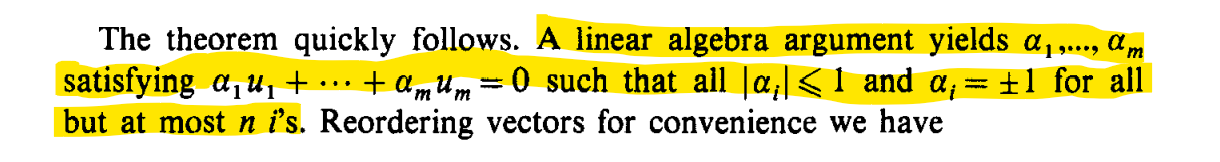
\includegraphics[scale=1.3]{Joel_Spencer_balancing_vectors.png}\retTwo\par}

Our issue was figuring out what linear algebra argument Spencer was fucking using. After thinking about it for three days while I was grading tests, I finally came up with a proof:\retTwo

\Hstatement\blab{Theorem:} Let $u_1, \ldots, u_m$ be vectors in $\mathbb{R}^n$. Then there are constants $a_1, \ldots, a_m$ satisfying\\ $a_1u_1 + \ldots + a_mu_m = 0$ such that all $|a_i| \leq 1$ and $a_i = \pm 1$ for all but at most $n$ $i$'s.

\begin{myIndent}\HexOne
	Proof:\\
	We'll proceed by an inductive argument. For our base case, let $u_{m+1} \coloneq 0$. That way\\ $\sum_{i = 1}^m 0 u_i = u_{m+1}$. Next, suppose that for $n + 1 \leq k \leq m$, we've shown that there\\ are constants $b_1, \ldots, b_{k} \in [-1, 1]$ and $\varepsilon_{k+1}, \ldots, \varepsilon_{m+1} \in \{-1, +1\}$ satisfying that:

	{\centering $b_1u_1 + \ldots + b_ku_k = \varepsilon_{k+1}u_{k+1} + \ldots + \varepsilon_{m+1}u_{m+1}$. \retTwo\par}

	If we consider the matrix $U \coloneqq \begin{bmatrix}u_1 & \cdots & u_k\end{bmatrix}$, then letting $b = (b_1, \ldots, b_k)$ we have that any $a = (a_1, \ldots, a_k) \in b + \ker(U)$ will satisfy that:
	
	{\centering $a_1u_1 + \ldots + a_{k}u_{k} = \varepsilon_{k+1}u_{k+1} + \ldots + \varepsilon_{m+1}u_{m+1}$.\retTwo\par}
	
	Since $k > n$, we know that $\ker(U)$ is nontrivial and hence unbounded. At the same time, $\|b\|_{\infty} \leq 1$. Hence, by the connectedness of $b + \ker(U)$ and the continuity of the $\infty$-norm, we know there is some $a \in b + \ker(U)$ with $\|a\|_\infty = 1$. After reordering our $u_i$, this is the same as saying that there exists $a_1, \ldots, a_{k-1} \in [-1, 1]$ and $\varepsilon_k = \pm 1$ such that:

	{\centering $a_1u_1 + \ldots + a_{k-1}u_{k-1} + \varepsilon_{k}u_k = \varepsilon_{k+1}u_{k+1} + \ldots + \varepsilon_{m+1}u_{m+1}$.\retTwo\par}
	
	Subtract both sides by $\varepsilon_{k}u_k$ to complete the induction step.\retTwo

	After induction, we will eventaully get constants $a_1, \ldots, a_n \in [-1, 1]$ and $\varepsilon_{n+1}, \ldots, \varepsilon_{m+1}$ equal to $\pm 1$ such that:

	{\centering $a_1u_1 + \ldots + a_nu_n = \varepsilon_{n+1}u_{n+1} + \ldots + \varepsilon_mu_m + \varepsilon_{m+1}u_{m+1}$. \retTwo\par}

	Move everything over to one side of the equation and forget about the $u_{m+1}$ and we have proven what we wanted.\newpage
\end{myIndent}

\dispDate{8/6/2025}\hOne

Now I'm going to go back to studying tensors.\retTwo

A \udefine{multi-index of length $k$} is a $k$-tuple $I = (i_1, \ldots, i_k)$ of integers. We say $I$ is a multi-index of $n$ if each $i$ is between $1$ and $n$. Now let $u_1, \ldots, u_n$ is a basis of $V$. For $T \in \mathcal{L}^k(V)$, write $T_I \coloneq T(u_{i_1}, \ldots, u_{i_k})$ for every multi-index $I$ of $n$ of length $k$.\retTwo

\exOne\ul{Proposition 1.3.7:} The $T_I$ uniquely determine $T$.

\begin{myIndent}\exTwoP
	Proof:\\
	When $k = 1$, $T$ is just a linear map and we've already proven this for linear maps. For $k > 1$, we proceed by induction. For each $i$, define $T_i \in L^{k-1}(V)$ by:
	
	{\centering $(v_1, \ldots, v_{k-1}) \mapsto T(v_1, \ldots, v_{k-1}, u_i)$.\retTwo\par} Then for $v = c_1u_1 + \ldots + c_nu_n$, we have:

	{\centering $T(v_1, \ldots, v_{k-1}, v) = \sum\limits_{i=1}^n c_iT_i(v_1, \ldots, v_{k-1})$\retTwo\par}

	Also, by induction each $T_i$ is uniquely determined by the coefficients $T_I$ where $I$ is a multi-index of $n$ of length $k$ with a final index equal to $i$.\retTwo

	\begin{myIndent}\exPPP
		Side note: We can see that if $C = (c_{i,j}) \in \mathcal{M}_{n \times k}(F)$ is the matrix satisfying that $v_{j} = \sum_{i=1}^n c_{i,j} u_i$ for each $j$, then:

		{\centering $T(v_1, \ldots, v_k) = \hspace{-1em}\sum\limits_{I = (i_1, \ldots, i_k)}\hspace{-0.5em} \left(\hspace{0.1em}\prod\limits_{j=1}^k c_{i_j, j}\right)T_I$ \retTwo\par}
	\end{myIndent}
\end{myIndent}

\hOne%
Given two tensors: $T_1 \in \mathcal{L}^k(V)$ and $T_2 \in \mathcal{L}^\ell(V)$, we define the \udefine{tensor product} of $T_1$ and $T_2$ as:

{\centering $(T_1 \otimes T_2)(v_1, \ldots, v_k, v_{k+1}, \ldots, v_{k + \ell}) = T_1(v_1, \ldots, v_k)T_2(v_{k + 1}, \ldots, v_{k + \ell})$\retTwo\par}

Note that:\hTwo\\ [-20pt]
\begin{itemize}
	\item $\otimes$ is associative.
	\item If $T_1$ or $T_2$ is a $0$-tensor, then $\otimes$ is just scalar multiplication.
	\item If $\lambda \in F$, $T_1 \in \mathcal{L}^k(V)$, and $T_2 \in \mathcal{L}^\ell(V)$, then $\lambda(T_1 \otimes T_2) = (\lambda T_1) \otimes T_2 = T_1 \otimes (\lambda T_2)$.
	\item If $T_1, T_2 \in \mathcal{L}^k(V)$ and $T_3 \in \mathcal{L}^\ell(V)$, then $(T_1 + T_2) \otimes T_3 = (T_1 \otimes T_3) + (T_2 \otimes T_3)$. Also $T_3 \otimes (T_1 + T_2)  = (T_3 \otimes T_1 ) + (T_3 \otimes T_2)$\retTwo
\end{itemize}

\hOne Suppose $T \in \mathcal{L}^k(V)$ and there exists $\ell_1, \ldots, \ell_k \in V^* = \mathcal{L}^1(V)$ such that $T = \ell_1 \otimes \cdots \otimes \ell_k$. Then we say $T$ is \udefine{decomposable}.\retTwo

If $u_1, \ldots, u_n$ is a basis for $V$, then we can define the \udefine{dual basis}: $u_1^*, \ldots, u_n^*$ for $V^*$ such that if $v = \sum_{i=1}^n c_iu_i$, then $u_j^*(v) = c_j$.

\begin{myIndent}\exTwoP
	To prove that this is a basis, first note that if $f \in V^*$ and $\lambda_i = f(u_i)$, then we can easily see that for any $v = \sum_{i=1}^n c_iu_i$, then:\newpage
	
	{\centering $f(v) = \sum_{i=1}^n c_if(u_i) = \sum_{i=1}^n \lambda_ic_i = \sum_{i=1}^n \lambda_iu_i^*(v)$.\retTwo\par}

	It follow that $u_1^*, \ldots, u_n^*$ span all of $V^*$. Also, consider if $f = \sum_{i=1}^n \lambda_i u_i^* = 0$ where all the $\lambda_i \in F$. Then we know that $0 = f(u_j) = \lambda_j$ for all $j$. This shows that\\ $u_1^*, \ldots, u_n^*$ are linearly  independent.\retTwo
\end{myIndent}

\pracOne\mySepTwo
Tangent: if $V, W$ are vector fields over $F$ and $A: V \to W$ is a linear map, then we define the \udefine{transpose} $A^\dag: W^* \to V^*$ of $A$ by $f \mapsto A^\dag(f) = f \circ A$.\retTwo

\exOne\ul{Claim 1.2.15:} Suppose $e_1, \ldots, e_m$ is a basis of $V$ and $u_1, \ldots, u_n$ is a basis of $W$. Then if $A = (a_{i,j})$ is the the matrix of $A$ with respect to the given bases, we have that the matrix of $A^\dag$ with respect to the dual bases of $V$ and $W$ is given by $(a_{j,i})$.

\begin{myIndent}\exTwoP
	Proof:\\
	Suppose $(c_{j,i})$ is the matrix representation of $A^\dag$. Then:

	{\centering $A^\dag(u_i^*)(e_j) = u_i^*(A(e_j)) = u_i^*(\sum_{k=1}^n a_{k,j}u_k) = a_{i,j}$ \retTwo\par}

	Simultaneously:

	{\centering $A^\dag(u_i^*)(e_j) = \sum_{k=1}^m c_{k, i} e_k^*(e_j) = c_{j, i}$ \retTwo\par}
\end{myIndent}
\pracOne\mySepTwo

\hOne Let $u_1, \ldots, u_n$ be a basis of $V$ and $u_1^*, \ldots, u_n^*$ be the corresponding dual basis of $V^*$. Then for every multi-index $I = (i_1, \ldots, i_k)$ of $n$ of length $k$, define:

{\centering $u_I^* = u_{i_1}^* \otimes \cdots \otimes u_{i_k}^*$.\retTwo\par}

Note that if $J = (j_1, \ldots, j_k)$ is another multi-index of $n$ of length $k$, then\\ $u_I^*(u_{j_1}, \ldots, u_{j_k}) = \delta_{I,J}$ where $\delta$ is the Kronecker delta function.\retTwo

\exOne\ul{Theorem 1.3.13:} The $k$-tensors $u_I^*$ form a basis for $\mathcal{L}^k(V)$.
\begin{myIndent}\exTwoP 
	Proof:\\
	Suppose $T \in \mathcal{L}^k(V)$. Then if $T^\prime \coloneq \sum_{I} T_Iu_I^*$, we have that $T^\prime_J = T_J$ for all multi-indices $J$ of $n$ of length $k$. Therefore, since $T^\prime$ and $T$ are uniquely determined by the same $T_I$, this proves that $T = T^\prime$. So, $T$ is in the span of the $u_I^*$. This proves that the $u_I^*$ span all of $\mathcal{L}^k(V)$.\retTwo

	Next suppose $T^\prime = \sum_{I} C_Iu_I^* = 0$ where each $C_I \in F$. Then if $J$ is a multi-index of $n$ of length $k$,
	
	{\centering$0 = T^\prime(u_{j_1}, \ldots, u_{j_k}) = \sum\limits_{I} C_Iu_I^*(u_{j_1}, \ldots, u_{j_k}) = C_J$\retTwo\par}

	This shows that the $u_I^*$ are linearly independent. \blacksquare\retTwo
\end{myIndent}

\ul{Corollary 1.3.15:} If $V$ is an $n$-dimensional vector space, then $\mathcal{L}^k(V)$ is an\\ $n^k$-dimensional vector space.\newpage

\hOne If $V, W$ are vector fields over $F$, $A: V \to W$ is a linear map, and $T \in \mathcal{L}^k(W)$, we define $A^\dag T(v_1, \ldots, v_k) \coloneq T(Av_1, \ldots, Av_k)$.\retTwo

We call $A^\dag T$ the \udefine{pullback} of $T$ by the map $A$. Note that this is just a generalization of taking the transpose of $A$.\retTwo

\exOne\ul{Proposition 1.3.18:} If we denote $A^\dag : \mathcal{L}^k(W) \to \mathcal{L}^k(V)$ to be the map $T \mapsto A^\dag T$, then $A^\dag$ is a linear map.

\begin{myIndent}\exTwoP This should be pretty obvious\dots\retTwo
\end{myIndent}

Furthermore, $A^\dag(T_1 \otimes T_2) = (A^\dag T_1) \otimes (A^\dag T_2)$.

\begin{myIndent}\exTwoP
	Proof:\\
	Suppose $T_1 \in \mathcal{L}^k(V)$ and $T_2 \in \mathcal{L}^\ell(V)$. Then:

	{\centering\begin{tabular}{l}
		$A^\dag(T_1 \otimes T_2)(v_1, \ldots, v_k, v_{k+1}, \ldots, v_{k+\ell})$\\
		$\phantom{aaaaaaaaaaaaaa} = (T_1 \otimes T_2)(Av_1, \ldots, Av_k, Av_{k+1}, \ldots, Av_{k+\ell})$\\
		$\phantom{aaaaaaaaaaaaaa} = T_1(Av_1, \ldots, Av_k)T_2(Av_{k+1}, \ldots, Av_{k+\ell})$\\
		$\phantom{aaaaaaaaaaaaaa} = A^\dag T_1(v_1, \ldots, v_k)A^\dag T_2(v_{k+1}, \ldots, v_{k+\ell})$\\
		$\phantom{aaaaaaaaaaaaaa} = (A^\dag T_1 \otimes A^\dag T_2)(v_1, \ldots, v_k, v_{k+1}, \ldots, v_{k+\ell})$. $\blacksquare$
	\end{tabular}\retTwo\par}
\end{myIndent}

As a corollary to the above fact, we know that pullbacks map decomposable tensors to decomposable tensors.\retTwo

Finally, suppose $B: U \to V$ is another linear map. Then $(AB)^\dag T = B^\dag(A^\dag T)$ for all $T \in \mathcal{L}^k(W)$. In other words, $(AB)^\dag = B^\dag A^\dag$.

\begin{myIndent}\exTwoP
	Proof:

	{\centering\begin{tabular}{l}
		$B^\dag(A^\dag T)(v_1, \ldots, v_k) = A^\dag T(Bv_1, \ldots, Bv_k)$\\
		$\phantom{B^\dag(A^\dag T)(v_1, \ldots, v_k)} = T(ABv_1, \ldots, ABv_k) = (AB)^\dag T(v_1, \ldots, v_k)$. $\blacksquare$
	\end{tabular}\retTwo\par}
\end{myIndent}

\hOne\blab{Alternating $k$-Tensors:}\\
Let $V$ be an $n$-dimensional vector space over a field $F$ with characteristic $\neq 2$ and $S_k$ be the symmetric group over $\{1, \ldots, k\}$. For $\sigma \in S_k$ and $T \in \mathcal{L}^k(V)$, we define $T^\sigma \in \mathcal{L}^k(V)$ by:

{\centering $T^\sigma(v_1, \ldots, v_k) = T(v_{\sigma^{-1}(1)}, \ldots, v_{\sigma^{-1}(k)})$ \retTwo\par}

\exOne\ul{Proposition 1.4.14:}
\begin{itemize}
	\item[(a)] If $T = \ell_1 \otimes \cdots \otimes \ell_k$ where each $\ell_i \in V^*$, then $T^\sigma = \ell_{\sigma(1)} \otimes \cdots \otimes \ell_{\sigma(k)}$.
	
	\begin{myIndent}\exTwoP
		Proof:

		{\centering\begin{tabular}{l}
			$T^\sigma(v_1, \ldots, v_k) = T(v_{\sigma^{-1}(1)}, \ldots, v_{\sigma^{-1}(k)}) = \ell_1(v_{\sigma^{-1}(1)}) \cdots \ell_k(v_{\sigma^{-1}(k)})$\\
			$\phantom{T^\sigma(v_1, \ldots, v_k) = T(v_{\sigma^{-1}(1)}, \ldots, v_{\sigma^{-1}(k)})} = \ell_{\sigma(1)}(v_1) \cdots \ell_{\sigma(k)}(v_k)$\\
			$\phantom{T^\sigma(v_1, \ldots, v_k) = T(v_{\sigma^{-1}(1)}, \ldots, v_{\sigma^{-1}(k)})} = (\ell_{\sigma(1)} \otimes \cdots \otimes \ell_{\sigma(k)})(v_1, \ldots, v_k)$
		\end{tabular}\retTwo\par}
	\end{myIndent}

	\item[(b)] If $\sigma \in S_k$, the function $T \mapsto T^\sigma$ is a linear map from $\mathcal{L}^k(V)$ to $\mathcal{L}^k(V)$.
	\begin{myIndent}\exTwoP
		This should be obvious. Also note that this map is invertible via the function $T \mapsto T^{(\sigma^{-1})}$.\newpage
	\end{myIndent}

	\item[(c)] If $\sigma, \tau \in S_k$, then $(T^\sigma)^\tau = T^{\sigma \tau}$.
	
	\begin{myIndent}\exTwoP
		Proof:\\
		Let $u_i \coloneq v_{\tau^{-1}(i)}$ for all $i$. Then:

		{\centering\begin{tabular}{l}
			$(T^\sigma)^\tau(v_1, \ldots, v_k) = T^\sigma(v_{\tau^{-1}(1)}, \ldots, v_{\tau^{-1}(k)})$\\ [2pt]

			$\phantom{(T^\sigma)^\tau(v_1, \ldots, v_k)} = T^\sigma(u_1, \ldots, u_k) = T(u_{\sigma^{-1}(1)}, \ldots, u_{\sigma^{-1}(k)})$\\ [2pt]

			$\phantom{(T^\sigma)^\tau(v_1, \ldots, v_k) = T^\sigma(u_1, \ldots, u_k)} = T(v_{\tau^{-1}(\sigma^{-1}(1))}, \ldots, v_{\tau^{-1}(\sigma^{-1}(k))})$\\ [2pt]

			$\phantom{(T^\sigma)^\tau(v_1, \ldots, v_k) = T^\sigma(u_1, \ldots, u_k)} = T(v_{(\sigma\tau)^{-1}(1)}, \ldots, v_{(\sigma\tau)^{-1}(k)})$\\ [2pt]

			$\phantom{(T^\sigma)^\tau(v_1, \ldots, v_k) = T^\sigma(u_1, \ldots, u_k)} = T^{\sigma\tau}(v_1, \ldots, v_k)$
		\end{tabular}\retTwo\par}
	\end{myIndent}
\end{itemize}

\hOne Let $V$ be a vector space and $k \geq 1$ be an integer. Then $T \in \mathcal{L}^k(V)$ is \udefine{alternating} if $T^\sigma = \sgn(\sigma)T$ for all $\sigma \in S_k$. We denote $\mathcal{A}^k(V)$ as the set of all alternating\\ $k$-tensors on $V$.

\begin{myIndent}\hTwo
	Note:
	\begin{itemize}
		\item If $c_1, c_2 \in F$ and $T_1, T_2 \in \mathcal{A}^k(V)$, then since $T \mapsto T^\sigma$ is a linear map, we have for all $\sigma \in S_k$ that:
		
		{\centering\begin{tabular}{l}
			$(c_1T_1 + c_2T_2)^{\sigma} = c_1T_1^{\sigma} + c_2T_2^\sigma$\\
			$\phantom{(c_1T_1 + c_2T_2)^{\sigma}} = c_1\sgn(\sigma)T_1 + c_2\sgn(\sigma)T_2 = \sgn(\sigma)(c_1T_1 + c_2T_2)$
		\end{tabular}\retTwo\par}

		This proves that $\mathcal{A}^k(V)$ is a subspace of $\mathcal{L}^k(V)$.\retTwo

		\item We shall define $\mathcal{A}^0(V) \coloneqq \mathcal{L}^0(V) = F$.\retTwo
	\end{itemize}
\end{myIndent}

Given an integer $k > 0$, and a tensor $T \in \mathcal{L}^k(V)$, let:

{\centering $\Alt(T) \coloneqq \sum\limits_{\tau \in S_k} \sgn(\tau)T^\tau$.\retTwo\par}

Then the \udefine{alternation operation} has the following properties:\\
\exOne\ul{Proposition 1.4.17:}
\begin{itemize}
	\item[(a)] Given any $T \in \mathcal{L}^k(V)$ and $\sigma \in S_k$ (where $k > 0$), we have that\\ $(\Alt(T))^{\sigma} = \sgn(\sigma)\Alt(T)$. I.e., $\Alt(T)$ is an alternating tensor.
	
	\begin{myIndent}\exTwoP
		Proof:\\
		By proposition 1.4.14 plus the fact that $(\sgn(\sigma))^2 = 1$, we have that:

		{\centering\begin{tabular}{l}
			$(\Alt(T))^\sigma = (\sum\limits_{\tau \in S_k}\sgn(\tau)T^{\tau})^{\sigma}$\\ [16pt]
		
			$\phantom{(\Alt(T))^\sigma} = 1 \cdot \hspace{-0.4em}\sum\limits_{\tau \in S_k}\sgn(\tau)T^{\tau\sigma} = (\sgn(\sigma))^2 \sum\limits_{\tau \in S_k}\sgn(\tau)T^{\tau\sigma}$\\ [16pt]

			$\phantom{(\Alt(T))^\sigma = 1 \cdot \hspace{-0.4em}\sum\limits_{\tau \in S_k}\sgn(\tau)T^{\tau\sigma}} = \sgn(\sigma) \sum\limits_{\tau \in S_k}\sgn(\tau\sigma)T^{\tau\sigma} = \sgn(\sigma) \sum\limits_{\tau^\prime \in S_k}\sgn(\tau^\prime)T^{\tau^\prime}$\\ [16pt]

			$\phantom{(\Alt(T))^\sigma = 1 \cdot \hspace{-0.4em}\sum\limits_{\tau \in S_k}\sgn(\tau)T^{\tau\sigma} = \sgn(\sigma) \sum\limits_{\tau \in S_k}\sgn(\tau\sigma)T^{\tau\sigma}} = \sgn(\sigma) \Alt(T)$\\ [16pt]
		\end{tabular} \newpage\par}
	\end{myIndent}

	\item[(b)] If $T \in \mathcal{A}^k(V)$, the $\Alt(T) = k!T$.
	
	\begin{myIndent}\exTwoP
		Proof:\\
		Since $T^\tau = \sgn(\tau)T$ for all $\tau \in S_k$, we know:

		{\centering\begin{tabular}{l}
			$\Alt(T) = \sum\limits_{\tau \in S_k} \sgn(\tau)T^\tau = \sum\limits_{\tau \in S_k} (\sgn(\tau))^2T = \sum\limits_{\tau \in S_k} (1)T = |S_k|T = k!T$
		\end{tabular} \retTwo\par}
	\end{myIndent}

	\item[(c)] $\Alt(T^\sigma) = (\Alt(T))^\sigma$.
	
	\begin{myIndent}\exTwoP
		Proof:\\
		By similar reasoning to in part (a), we have that:

		{\centering\begin{tabular}{l}
			$\Alt(T^\sigma) = 1 \cdot \hspace{-0.4em}\sum\limits_{\tau \in S_k} \sgn(\tau) T^{\sigma\tau} = (\sgn(\sigma))^2 \sum\limits_{\tau \in S_k} \sgn(\tau) T^{\sigma\tau}$\\ [12pt]

			$\phantom{\Alt(T^\sigma) = 1 \cdot \hspace{-0.4em}\sum\limits_{\tau \in S_k} \sgn(\tau) T^{\sigma\tau}} = \sgn(\sigma) \sum\limits_{\tau \in S_k} \sgn(\sigma\tau) T^{\sigma\tau}$\\ [12pt]

			$\phantom{\Alt(T^\sigma) = 1 \cdot \hspace{-0.4em}\sum\limits_{\tau \in S_k} \sgn(\tau) T^{\sigma\tau}} = \sgn(\sigma) \sum\limits_{\tau^\prime \in S_k} \sgn(\tau^\prime) T^{\tau^\prime} = \sgn(\sigma)\Alt(T)$
		\end{tabular} \retTwo\par}

		And since $\sgn(\sigma)\Alt(T) = (\Alt(T))^\sigma$ by part (a), we know $\Alt(T^\sigma) = (\Alt(T))^\sigma$.\retTwo
	\end{myIndent}

	\item[(d)] The map $\Alt: \mathcal{L}^k(V) \to \mathcal{L}^k(V)$ defined by $T \mapsto \Alt(T)$ is a linear map. (Also it's onto if $F$ has characteristic $0$ or $> k$.)
	
	\begin{myIndent}\exTwoP
		Proof:\\
		$\Alt$ is a linear map because it is a linear combination of a bunch of linear maps. The onto property follows from part (b).\retTwo
	\end{myIndent}
\end{itemize}

\hOne\dispDate{8/7/2025}

If $I = (i_1, \ldots, i_k)$ is a multi-index of $n$ of length $k$, then we write:
\begin{itemize}
	\item $I$ is \udefine{repeating} if $i_s = i_r$ for some $s \neq r$.
	\item $I$ is \udefine{increasing} if $i_1 < i_2 < \ldots < i_k$.
	\item Given $\sigma \in S_k$, we define $I^\sigma = (i_{\sigma(1)}, \ldots, i_{\sigma(k)})$.\retTwo
\end{itemize}

Note that if $I$ is not repeating, then there is a unique permutation $\sigma \in S_k$ such that $I^\sigma$ is increasing.\retTwo

Let $u_1, \ldots, u_n$ be a basis of the vector space $V$ over a field $F$ of characteristic $\neq 2$, and let $u_1^*, \ldots, u_n^*$ be the corresponding dual basis. Now given the multi-index\\ $I = (i_1, \ldots, i_k)$, set $u_I^* = u_{i_1}^* \otimes \cdots \otimes u_{i_k}^*$. Next define $\Psi_I = \Alt(u_I^*)$.\retTwo

\exOne\ul{Proposition 1.4.20:} Let $I = (i_1, \ldots, i_k)$ and $J = (j_1, \ldots, j_k)$ be multi-indices.
\begin{itemize}
	\item[(a)] $\Psi_{I^\sigma} = \sgn(\sigma)\Psi_I$.
	\begin{myIndent}\exTwoP
		To start off, by the last proposition:
		
		{\centering$\sgn(\sigma)\Psi_I = \sgn(\sigma)\Alt(u_I^*) = (\Alt(u_I^*))^\sigma = \Alt((u_I^*)^\sigma)$.\newpage\par}

		Next, set $\ell_j = u^*_{i_j}$ for $1 \leq j \leq k$. Then by proposition 1.4.14, we have:
		
		{\centering$(u_I^*)^\sigma = (\ell_1 \otimes \cdots \otimes \ell_k)^\sigma = \ell_{\sigma(1)} \otimes \cdots \otimes \ell_{\sigma(k)} = u_{i_{\sigma(1)}}^* \otimes \cdots \otimes u_{i_{\sigma(k)}}^* = u^*_{I^\sigma}$.\retTwo\par}

		Thus $\sgn(\sigma)\Psi_I = \Alt((u_I^*)^\sigma) = \Alt(u^*_{I^\sigma}) = \Psi_{I^\sigma}$.\retTwo
	\end{myIndent}

	\item[(b)] If $I$ is repeating, $\Psi_{I} = 0$.
	
	\begin{myIndent}\exTwoP
		If $I$ is repeating, then there exists $r \neq s$ such that $i_r = i_s$. Then in turn, if $\tau_{r,s} \in S_k$ is the transposition of $r$ and $s$, then $\sgn(\tau_{r,s}) = -1$ and $I^{\tau_{r,s}} = I$. Then by part (a), we have:

		{\centering$\Psi_I = \Psi_{I^{\tau_{r,s}}} = \sgn(\tau_{r,s})\Psi_{I} = -\Psi_{I}$\retTwo\par}
		
		This is only possible if $\Psi_I(v_1, \ldots, v_k) = 0$ for all $v_1, \ldots, v_k \in V$. Hence $\Psi_I$ is the zero map.\retTwo
	\end{myIndent}


	\item[(c)] If $I$ and $J$ are strictly increasing, then $\Psi_I(u_{j_1}, \ldots, u_{j_k}) = \delta_{I,J}$ where $\delta$ is the Kronecker delta function.
	
	\begin{myIndent}\exTwoP
		To start off, note that:

		{\centering\begin{tabular}{l}
			$\Psi_I(u_{j_1}, \ldots, u_{k_k}) = \sum\limits_{\tau \in S_k}\sgn(\tau)(u_I^*)^{\tau}(u_{j_1}, \ldots, u_{j_k})$\\ [18pt]

			$\phantom{\Psi_I(u_{j_1}, \ldots, u_{k_k})} = \sum\limits_{\tau \in S_k}\sgn(\tau)(u_{i_1}^* \otimes \cdots \otimes u_{i_k}^*)^{\tau}(u_{j_1}, \ldots, u_{j_k})$\\ [18pt]

			$\phantom{\Psi_I(u_{j_1}, \ldots, u_{k_k})} = \sum\limits_{\tau \in S_k}\sgn(\tau)(u_{i_{\tau(1)}}^* \otimes \cdots \otimes u_{i_{\tau(k)}}^*)(u_{j_1}, \ldots, u_{j_k})$\\ [18pt]

			$\phantom{\Psi_I(u_{j_1}, \ldots, u_{k_k})} = \sum\limits_{\tau \in S_k}\sgn(\tau)u_{i_{\tau(1)}}^*(u_{j_1})\cdots u_{i_{\tau(k)}}^*(u_{j_k})$\\ [18pt]
		\end{tabular}\retTwo\par}

		Now it's clear that $u_{i_{\tau(1)}}^*(u_{j_1})\cdots u_{i_{\tau(k)}}^*(u_{j_k}) = \delta_{I^\tau, J}$. Also, since both $J$ and $I$ are strictly increasing and also since there is only one permutation such that $I^\sigma$ is strictly increasing for any nonrepeating $I$, we know that $\delta_{I^\tau, J} = 1$ iff $\tau = \myId$ and $I = J$. And in that case $\sgn(\tau) = 1$. Hence: 
		
		{\centering $\sum\limits_{\tau \in S_k}\sgn(\tau)u_{i_{\tau(1)}}^*(u_{j_1})\cdots u_{i_{\tau(k)}}^*(u_{j_k}) = \delta_{I,J}$.\retTwo\par}
	\end{myIndent}
\end{itemize}

\ul{Proposition 1.4.24:} Suppose $F$ has characteristic $0$ or greater than $k$. Then\\ $\{\Psi_J : J \text{ is increasing}\}$ is a basis for $\mathcal{A}^k(V)$.

\begin{myIndent}\exTwoP
	Proof:\\
	Suppose $T \in \mathcal{A}^k(V)$. By theorem 1.3.13, we know there exists $a_I \in F$ such that $T = \sum_{I} a_I u_I^*$. However, we also know that $k!T = \Alt(T)$. Since $\Alt$ is a linear map, we thus know that:

	{\centering $T = \frac{1}{k!}\Alt(T) = \sum\limits_I \frac{a_I}{k!} \Alt(u_I^*) = \sum\limits_I \frac{a_I}{k!} \Psi_I$\newpage\par}

	If $I$ is repeating, then $\frac{a_I}{k!} \Psi_I^*$  cancels. Otherwise, there is some $\sigma \in S_k$ and some increasing multi-index $J$ such that:
	
	{\centering $\frac{a_I}{k!} \Psi_I = \frac{a_I}{k!} \Psi_{J^\sigma} = \frac{a_I\sgn(\sigma)}{k!} \Psi_{J}$.\retTwo\par}

	By collecting terms, we get that $T = \hspace{-1em}\sum\limits_{J \text{ increasing}}\hspace{-1em}c_J\Phi_J$ where each $c_J \in F$.\retTwo

	This shows that the $\Psi_J$ span all of $\mathcal{A}^k(V)$. Next we show that they form a basis.\\ Suppose $T = \hspace{-1em}\sum\limits_{J \text{ increasing}}\hspace{-1em}c_J\Phi_J = 0$.\retTwo

	Then by part (c) of the last proposition, we know that if $I = (i_1, \ldots, i_k)$ is an\\ increasing multi-index, then:

	{\centering $0 = T(u_{i_1}, \ldots, u_{i_k}) = C_I$ \retTwo\par}

	So, all the $C_I$ are equal to $0$. $\blacksquare$\retTwo
\end{myIndent}

\ul{Corollary:} If $F$ has characteristic $0$ or greater than $k$, then $\mathcal{A}^k(V)$ has dimension $\binom{n}{k}$.\retTwo

\ul{Corollary 2:} If $F$ has characteristic $0$ or greater than $k \geq n$, then any alternating $n$-tensor on $V$ is a scalar multiple of a determinant function. Also, there are no\\ nontrivial alternating $m$-tensors where $n < m \leq k$.\retTwo

\pracOne\ul{Exercise 1.4.ix:} Suppose $A: V \to W$ is a linear map. Then if $T \in \mathcal{A}^k(W)$, we have that $A^\dag T \in \mathcal{A}^k(V)$. Hence, the pullback operation maps alternating tensors to alternating tensors.

\begin{myIndent}\pracTwo
	Proof:\\
	Suppose $\sigma \in S_k$. Then for any $v_1, \ldots, v_k \in V$, we have that:

	{\centering\begin{tabular}{l}
		$(A^\dag T)^\sigma(v_1, \ldots, v_k) = A^\dag T(v_{\sigma^{-1}(1)}, \ldots, v_{\sigma^{-1}(k)})$\\ [6pt]

		$\phantom{(A^\dag T)^\sigma(v_1, \ldots, v_k)} = T(Av_{\sigma^{-1}(1)}, \ldots, Av_{\sigma^{-1}(k)})$\\ [6pt]

		$\phantom{(A^\dag T)^\sigma(v_1, \ldots, v_k)} = T^\sigma(Av_1, \ldots, Av_k)$\\ [6pt]

		$\phantom{(A^\dag T)^\sigma(v_1, \ldots, v_k)} = \sgn(\sigma)T(Av_1, \ldots, Av_k) = \sgn(\sigma)A^\dag T(v_1, \ldots, v_k)$
	\end{tabular}\retTwo\par}

	Hence, $(A^\dag T)^\sigma = \sgn(\sigma)A^\dag T$. This proves that $A^\dag T$ is alternating. $\blacksquare$\retTwo
\end{myIndent}

\ul{Exercise 1.4.x:} Additionally to the last exercise, we have that if $T \in \mathcal{L}^k(V)$, then\\ $A^\dag(\Alt(T)) = \Alt(A^\dag T)$.

\begin{myIndent}\pracTwo
	Proof:\\
	If $v_1, \ldots, v_k \in V$, then:

	{\centering\begin{tabular}{l}
		$\Alt(A^\dag T)(v_1, \ldots, v_k) = \sum\limits_{\tau \in S_k}\sgn(\tau)(A^\dag T )^\tau(v_1, \ldots, v_k)$\\ [16pt]

		$\phantom{\Alt(A^\dag T)(v_1, \ldots, v_k)} = \sum\limits_{\tau \in S_k}\sgn(\tau)A^\dag T(v_{\tau^{-1}(1)}, \ldots, v_{\tau^{-1}(k)})$\\ [16pt]

		$\phantom{\Alt(A^\dag T)(v_1, \ldots, v_k) } = \sum\limits_{\tau \in S_k}\sgn(\tau)T(Av_{\tau^{-1}(1)}, \ldots, Av_{\tau^{-1}(k)})$\\ [-24pt]

		$\phantom{\Alt(A^\dag T)(v_1, \ldots, v_k) = \Alt(T)(Av_1, \ldots, Av_k) = A^\dag(\Alt (T))(v_1, \ldots, v_k)}$
	\end{tabular}\newpage
	
	\begin{tabular}{l}
		$\phantom{\Alt(A^\dag T)(v_1, \ldots, v_k)} = \sum\limits_{\tau \in S_k}\sgn(\tau)T^\tau(Av_1, \ldots, Av_k)$\\ [16pt]

		$\phantom{\Alt(A^\dag T)(v_1, \ldots, v_k) } = \Alt(T)(Av_1, \ldots, Av_k) = A^\dag(\Alt (T))(v_1, \ldots, v_k)$
	\end{tabular}\retTwo\par}

	This shows that $\Alt(A^\dag T) =  A^\dag(\Alt (T))$. $\blacksquare$\retTwo
\end{myIndent}

\hOne\blab{The space $\Lambda^k(V^*)$:}\\
If $k > 1$, a decomposable $k$-tensor $\ell_1 \otimes \cdots \otimes \ell_k$ with each $\ell_i \in V^*$ is called \udefine{redundant} if $\ell_i = \ell_{i+1}$ for some index $i$. We let $\mathcal{I}^k(V)$ be the span of all redundant $k$-tensors.

\begin{myIndent}\hTwo 
	If $k = 1$, we define $\mathcal{I}^1(V) \coloneq \{0\} \subseteq \mathcal{L}^1(V)$.\\ Also if $k = 0$, we define $\mathcal{I}^0(V) \coloneq \{0\} \subseteq F$.\retTwo 
\end{myIndent}

\exOne\ul{Proposition 1.5.2:} Suppose $F$ has characteristic $\neq 2$. If $T \in \mathcal{I}^k(V)$, then $\Alt(T) = 0$. In other words, $\mathcal{I}^k(V) \subseteq \ker(\Alt)$.

\begin{myIndent}\exTwoP
	Proof:\\
	If $T \in \mathcal{I}^k(V)$, then we know there are redundant decomposable $k$-tensors\\ $T_1, \ldots, T_m$ as well as scalars $c_1, \ldots, c_m \in F$ such that $T = \sum_{j=1}^m c_jT_j$. Then since\\ $\Alt(T) = \sum_{j=1}^m c_j\Alt(T_j)$, all we need to do now is show that $\Alt(T_j) = 0$ for\\ every $j$.\retTwo

	Since $T_j$ is a redundant decomposable $k$-tensor, we know that $T_j = \ell_1 \otimes \cdots \otimes \ell_k$ where $\ell_i = \ell_{i+1}$ for some $1 \leq i < k$. In turn, if $\tau_{i, i+1} \in S_k$ is the transposition of $i$ and $i+1$, we have that $(T_j)^{\tau_{i,i+1}} = T_j$ and $\sgn(\tau_{i, i+1}) = -1$. Hence:

	{\centering$\Alt(T_j) = \Alt((T_j)^{\tau_{i, i+1}}) = \sgn(\tau_{i,i+1})\Alt(T_j) = -\Alt(T_j)$\retTwo\par}

	This implies that $\Alt(T_j) = 0$. $\blacksquare$\retTwo
\end{myIndent}

\ul{Proposition 1.5.3:} If $T \in \mathcal{I}^r(V)$ and $T^\prime \in \mathcal{L}^s(V)$, then $T \otimes T^\prime$ and $T^\prime \otimes T$ are in $\mathcal{I}^{r+s}(V)$.

\begin{myIndent}\exTwoP
	Proof:\\
	The argument for $T^\prime \otimes T$ being in $\mathcal{I}^{r+s}(V)$ is mostly identical to the argument for $T \otimes T^\prime$  being in $\mathcal{I}^{r+s}(V)$. So, I'll focus only on proving the latter.\retTwo

	To start off, like before we know that there are redundant decomposable $r$-tensors $T_1, \ldots, T_m$ as well as scalars $c_1, \ldots, c_m \in F$ such that $T = \sum_{j=1}^m c_jT_j$. Hence, it suffices to show that $T_j \otimes T^\prime \in \mathcal{I}^{r+s}(V)$ for all $1 \leq j \leq m$ since:

	{\center$T \otimes T^\prime = (\sum_{j=1}^m c_jT_j) \otimes T^\prime = \sum_{j=1}^m c_j (T_j \otimes T^\prime)$\retTwo\par}

	Fortunately, by writing $T^\prime = \sum_{I} d_Iu_I^*$, we can see that:

	{\centering $T_j \otimes T^\prime = T_j \otimes (\sum\limits_{I} d_I u_I^*) = \sum\limits_{I} d_I(T_j \otimes u_I^*)$\retTwo\par}

	Now since both $u_I^*$ and $T_j$ are decomposable and $T_j$ is redundant, we can easily see that $T_j \otimes u_I^*$ is decomposable and redundant. It follows that $T_j \otimes T^\prime \in \mathcal{I}^{r+s}(V)$. $\blacksquare$\retTwo
\end{myIndent}

\ul{Proposition 1.5.4:} Suppose $F$ has characteristic $\neq 2$. If $T \in \mathcal{L}^k(V)$ and $\sigma \in S_k$, then $T^\sigma = \sgn(\sigma)T + S$ where $S \in \mathcal{I}^k(V)$.\newpage

\begin{myIndent}\exTwoP
	Proof:\\
	Hopefully you're getting use to this trick. It suffices to assume $T$ is decomposable. After all, after writing $T = \sum_{I} c_Iu_I^*$, if we can show for all multi-indexes $I$ that $(u_{I}^*)^\sigma = \sgn(\sigma)u_{I}^* + S_I$ where $S_I \in \mathcal{I}^k(V)$, then we can set $S = \sum_{I} c_I S_I \in \mathcal{I}^k(V)$ and have that:

	{\centering $T^\sigma = \sum\limits_{I} c_I (u_I^*)^\sigma = \sgn(\sigma)\sum\limits_{I} c_I u_I^* + \sum\limits_{I} S_I = \sgn(\sigma)T + S$\retTwo\par}
	
	So suppose $T = \ell_1 \otimes \cdots \otimes \ell_k$. Then given $\sigma \in S^k$, we can write $\sigma = \tau_1 \ldots \tau_m$ as the product of $m$ many transpositions of adjacent pairs of numbers in $\{1, \ldots, k\}$.
	\begin{myIndent}\exPPP
		(by adjacent I mean a pair $\{j, j+1\}$ where $1 \leq j < k$\dots)\retTwo
	\end{myIndent}

	We shall induct on $m$. First assume $m = 1$. Thus $\sigma = \tau_{j,j+1}$ for some $1 \leq j < k$ and hence $\sgn(\sigma) = -1$. Also:

	{\centering\begin{tabular}{l}
		$T^\sigma -\sgn(\sigma)T = T^\sigma + T$\\ [3pt]

		$\phantom{T^\sigma -\sgn(\sigma)T} = (\ell_1 \otimes \cdots \otimes \ell_{j-1} \otimes \ell_{j+1} \otimes \ell_{j} \otimes \ell_{j+2} \otimes \cdots \otimes \ell_{k}) + (\ell_1 \otimes \cdots \otimes \ell_k)$\\ [3pt]

		$\phantom{T^\sigma -\sgn(\sigma)T} = (\ell_1 \otimes \cdots \otimes \ell_{j-1}) \otimes \left((\ell_{j+1} \otimes \ell_j) + (\ell_j \otimes \ell_{j+1})\right) \otimes (\ell_{j+2} \otimes \cdots \otimes \ell_{k})$
	\end{tabular}\retTwo\par}

	Now note that:

	{\centering\begin{tabular}{l}
		$(\ell_{j} + \ell_{j+1}) \otimes (\ell_{j} + \ell_{j+1}) = (\ell_j \otimes \ell_j) + (\ell_j \otimes \ell_{j+1}) + (\ell_{j+1} \otimes \ell_j) + (\ell_{j+1} \otimes \ell_{j+1})$.
	\end{tabular}\retTwo\par}

	Therefore:

	{\centering\begin{tabular}{l}
		$T^\sigma - \sgn(\sigma)T = (\ell_1 \otimes \cdots \otimes \ell_{j-1}) \otimes (\ell_j + \ell_{j+1}) \otimes (\ell_j + \ell_{j+1}) \otimes (\ell_{j+1} \otimes \cdots \otimes \ell_{k})$\\
		$\phantom{T^\sigma - \sgn(\sigma)T = aaaaaaaaaaa} - (\ell_1 \otimes \cdots \otimes \ell_{j-1}) \otimes \ell_j \otimes \ell_j \otimes (\ell_{j+2} \otimes \cdots \otimes \ell_{k})$\\
		$\phantom{T^\sigma - \sgn(\sigma)T = aaaaaaaaaaa} - (\ell_1 \otimes \cdots \otimes \ell_{j-1}) \otimes \ell_{j+1} \otimes \ell_{j+1} \otimes (\ell_{j+2} \otimes \cdots \otimes \ell_{k})$\\
	\end{tabular}\retTwo\par}

	Hence $T^\sigma - \sgn(\sigma)T \in \mathcal{I}^k(V)$ and we are done with this case.\retTwo

	Now suppose $m > 1$. Then $\sigma = \tau_{j,j+1} \sigma^\prime$ where $\sigma^\prime$ is the product of $m-1$\\ transpositions. By induction, we know that there exists $S_1 \in \mathcal{I}^k(V)$ such that:

	{\centering $T^\sigma = (T^{\tau_{j,j+1}})^{\sigma^\prime} = \sgn(\sigma^\prime)T^{\tau_{j,j+1}} + S_1$ \retTwo\par}

	Also by our base case, there is $S_2 \in \mathcal{I}^k(V)$ such that $T^{\tau_{j,j+1}} = \sgn(\tau_{j,j+1})T + S_2$. Then setting $S = \sgn(\tau_{j,j+1})S_2 + S_1$, we have that $S \in \mathcal{I}^K(V)$ and:

	{\centering $T^\sigma = \sgn(\sigma^\prime)(\sgn(\tau_{j,j+1})T + S_2) + S_1 = \sgn(\sigma)T + S$. $\blacksquare$\retTwo\par}
\end{myIndent}

\ul{Corollary 1.5.6:} Suppose $F$ has characteristic $\neq 2$. If $T \in \mathcal{L}^k(V)$, then\\ $\Alt(T) = k!T + S$ where $S \in \mathcal{I}^k(V)$.

\begin{myIndent}\exTwoP
	Proof:\\
	Given any $\tau \in S_k$, let $S_\tau \in \mathcal{I}^k(V)$ be such that $T^\tau = \sgn(\tau) T + S_\tau$. Then\\ $S \coloneq \sum_{\tau \in S_k} \sgn(\tau)S_\tau \in \mathcal{I}^k(V)$ and:

	{\center $\Alt(T) = \sum\limits_{\tau \in S_k}\sgn(\tau)T^\tau = \sum\limits_{\tau \in S_k} (\sgn(\tau))^2 T + \sum\limits_{\tau \in S_k} \sgn(\tau)S_{\tau} = k!T + S$. $\blacksquare$ \retTwo\par}
\end{myIndent}

\ul{Corollary 1.5.8:} Let $k \geq 1$. Then let $V$ be a vector space over a field $F$ of\\ characteristic $0$ or $> \max(k, 2)$. Then:

{\centering $\mathcal{I}^k(V) = \ker(\Alt: \mathcal{L}^k(V) \to \mathcal{A}^k(V))$ \retTwo\par}

\begin{myIndent}\exTwoP
	Proof:\\
	We already know from proposition 1.5.2 that $\mathcal{I}^k(V) \subseteq \ker(\Alt)$. To prove the\\ reverse relation, suppose $T \in \mathcal{L}^k(V)$ satisfies that $\Alt(T) = 0$. Then based on the previous corollary, we know there exists $S \in \mathcal{I}^k(V)$ such that $-\frac{1}{k!}S = T - \Alt(T)$. Hence $T \in \mathcal{I}^k(V)$. $\blacksquare$\retTwo
\end{myIndent}

\ul{Theorem 1.5.9:} Suppose $F$ is a field of characteristic $0$ or $> \max(k, 2)$. Then any element $T \in \mathcal{L}^k(V)$ can be written uniquely as a sum $T_1 + T_2$ where $T_1 \in \mathcal{A}^k(V)$ and $T_2 \in \mathcal{I}^k(V)$. I.e, $\mathcal{L}^k(V) = \mathcal{A}^k(V) \oplus \mathcal{I}^k(V)$.

\begin{myIndent}\exTwoP
	Proof:\\
	Let $W \in \mathcal{I}^k(V)$ satisfy that $\Alt(T) = k!T + W$. Then set $T_1 = \frac{1}{k!}\Alt(T)$ and\\ $T_2 = -\frac{1}{k!}W$. Then clearly $T = T_1 + T_2$ with $T_1 \in \mathcal{A}^k(V)$ and $T_2 \in \mathcal{I}^k(V)$.\retTwo

	Next, to prove uniqueness suppose $T^\prime_1 + T^\prime = T$ with $T^\prime_1 \in \mathcal{A}^k(V)$ and $T^\prime_2 \in \mathcal{I}^k(V)$. Then $T_1 - T^\prime_1 \in \mathcal{A}^k(V)$, $T_2 - T^\prime_2 \in \mathcal{I}^k(V)$, and $(T_1 - T^\prime_1) + (T_2 - T_2^\prime) = 0$. So:

	{\center $0 = \Alt(0) = \Alt((T_1 - T^\prime_1) + (T_2 - T_2^\prime)) = k!(T_1 - T^\prime_1)$ \retTwo\par}

	Hence $T_1 = T^\prime_1$ and it easily follows $T_2 = T^\prime_2$. $\blacksquare$\retTwo
\end{myIndent}

\hOne Let $k \geq 0$. Let $V$ be a finite dimensional vector space over a field $F$ of characteristic $0$ or $> \max(k, 2)$. Then we define:

{\centering $\Lambda^k(V^*) \coloneq \mathcal{L}^k(V) / \mathcal{I}^k(V)$ \retTwo\par}

By the first isomorphism theorem along with the previous theorem, we have that $\Lambda^k(V^*) \cong \mathcal{A}^k(V)$.\retTwo

\dispDate{8/8/2025}

Here is a tangent  about symmetric tensors. For this section, suppose $V$ is an\\ $n$-dimensional vector space over a field $F$ with characteristic $\neq 2$.\retTwo

A tensor $T \in \mathcal{L}^k(V)$ is \udefine{symmetric} if $T^\sigma = T$ for all $\sigma \in S_k$. We denote the space of\\ symmetric tensors $\mathcal{S}^k(V)$.
\begin{myIndent}\hTwo
	You can show by the same reasoning as with $\mathcal{A}^k(V)$ that $\mathcal{S}^k(V)$ is a vector subspace.\retTwo
\end{myIndent}

\pracOne\ul{Exercise 1.5.iii:} Suppose $F$ has characteristic $0$ or $> k$. Then if $T$ is a symmetric $k$-tensor and $k \geq 2$, we have that $T \in \mathcal{I}^k(V)$.

\begin{myIndent}\pracTwo
	Proof:\\
	Let $\sigma \in S_k$ be an odd permutation. Then by proposition 1.4.17:
	
	{\centering $\Alt(T) = \Alt(T^\sigma) = \sgn(\sigma)\Alt(T) = -\Alt(T)$.\newpage\par}

	The only way this is possible is if $\Alt(T) = 0$. Hence $T \in \ker(\Alt)$, and by theorem 1.5.8 that means that $T \in \mathcal{I}^k(V)$. $\blacksquare$\retTwo
\end{myIndent}

\hOne We define a \udefine{symmetrization} operator as follows. Given $T \in \mathcal{L}^k(V)$, define:

{\centering $\Sym(T) \coloneqq \sum\limits_{\sigma \in S_k} T^\sigma$ \retTwo\par}

Then like in proposition 1.4.17, we can show that given any $T \in \mathcal{L}^k(V)$ and $\sigma \in S_k$:
\begin{itemize}\hTwo
	\item[(a)] $(\Sym(T))^\sigma = \Sym(T)$ (i.e. $\Sym(T) \in \mathcal{S}^k(V)$\dots)
	\item[(b)] If $T \in \mathcal{S}^k(V)$, then $\Sym(T) = k!T$
	\item[(c)] $\Sym(T^\sigma) = \Sym(T)$
	\item[(d)] $\Sym: \mathcal{L}^k(V) \to \mathcal{A}^k(V)$ is an linear map (which is surjective so long as $k! \neq 0$ in the field $F$\dots).\retTwo 
\end{itemize}

Supposing $k! \neq 0$ in $F$, then by following a process very similar to what we did with the alternation operation, we can construct a basis for the symmetric tensors:

{\centering$\{\Phi_I^*: I \text{ is a non-decreasing multi-index}\}$.\retTwo\par}

\begin{myDindent}\pracTwo
	Note: By non-decreasing the textbook means that $I = (i_1, \ldots, i_k)$ satisfies that\\ $i_1 \leq i_2 \leq \cdots \leq i_k$.\retTwo
\end{myDindent}

I'm bored and won't do that construction here. But the important point is that this means $\mathcal{S}^k(V)$ has the same number of dimensions as there are non-decreasing multi-indexes of $n$ of length $k$. And since there are $\binom{n+k-1}{k}$ ways of picking $k$\\ elements of the set $\{1, \ldots, n\}$ when you allow yourself to pick the same element multiple times, this means that $\dim(\mathcal{S}^k(V)) = \binom{n+k-1}{k}$.

\begin{myIndent}\pracOne
	Side note: If $k! \neq 0$ in $F$, then we have already shown that $\dim(\mathcal{I}^k(V)) = n^k - \binom{n}{k}$. Since $\mathcal{S}^k(V) \subseteq \mathcal{I}^k(V)$, this shows that $\mathcal{S}^2(V) = \mathcal{I}^2(V)$. That said, we don't in general have that $\dim(\mathcal{I}^k(V)) = \dim(\mathcal{S}^k(V))$ when $k > 2$.\retTwo
\end{myIndent}

Next, here's some other miscellaneous results.\retTwo

\pracOne\ul{Exercise 1.5.vii:} Suppose $F$ has characteristic $0$ or $> \max(k, 2)$. Then if $T \in \mathcal{I}^k(V)$, we have that $T^\sigma \in \mathcal{I}^k(V)$ for all $\sigma \in S_k$.

\begin{myIndent}\pracTwo
	Proof:\\
	Since $T \in \mathcal{I}^k(V)$, we know that: $\Alt(T^\sigma) = \sgn(\sigma)\Alt(T) = 0$. Therefore,\\ $T^\sigma \in \ker(\Alt)$, and by corollary 1.5.8 we know that $\ker(\Alt) = \mathcal{I}^k(V)$. $\blacksquare$\retTwo
\end{myIndent}

\pracOne\ul{Corollary / Exercise 1.5.v:} Let $k \geq 2$ and suppose $F$ has characteristic $0$ or $> k$. Then if\\ $T \in \mathcal{L}^{k-2}(V)$ and $\ell \in V^*$, we have that $\ell \otimes T \otimes \ell \in \mathcal{I}^k(V)$.

\begin{myIndent}\pracTwo
	Proof:\\
	There is a permutation $\sigma \in S_k$ satisfying that $(\ell \otimes T \otimes \ell)^\sigma = (\ell \otimes \ell) \otimes T$. Then by proposition 1.5.3, we have that $(\ell \otimes \ell) \otimes T \in \mathcal{I}^k(V)$. And finally, by applying the last exercise we have that $\ell \otimes T \otimes \ell = ((\ell \otimes \ell) \otimes T)^{\sigma^{-1}} \in \mathcal{I}^k(V)$. $\blacksquare$\newpage
\end{myIndent}

\pracOne\ul{Corollary / Exercise 1.5.vi:} Let $k \geq 2$ and suppose $F$ has characteristic $0$ or $> k$. Then if\\ $T \in \mathcal{L}^{k-2}(V)$ and $\ell_1, \ell_2 \in V^*$, we have that $(\ell_1 \otimes T \otimes \ell_2) + (\ell_2 \otimes T \otimes \ell_1) \in \mathcal{I}^k(V)$.

\begin{myIndent}\pracTwo
	Proof:\\
	Apply the last exercise plus the fact that:

	{\centering\begin{tabular}{l}
	$(\ell_1 \otimes T \otimes \ell_2) + (\ell_2 \otimes T \otimes \ell_1) = ((\ell_1 + \ell_2) \otimes T \otimes (\ell_1 + \ell_2))$\\
	$\phantom{(\ell_1 \otimes T \otimes \ell_2) + (\ell_2 \otimes T \otimes \ell_1)aaaa} - (\ell_1 \otimes T \otimes \ell_1) - (\ell_2 \otimes T \otimes \ell_2)$. $\blacksquare$
	\end{tabular}\retTwo\par}
\end{myIndent}

\hOne\dispDate{8/9/2025}

\blab{The Wedge Product:}\\
In this section, we'll suppose $V$ is an $n$-dimensional vector space over a field $F$\\ of characteristic $0$. Also, we shall for each $k$ define the map $\pi: \mathcal{L}^k(V) \to \Lambda^k(V^*)$\\ such that $\pi(T) = T + \mathcal{I}^k(V)$ for all $T \in \mathcal{L}^k(V)$.\retTwo

Suppose for each $i \in \{1, 2\}$ we have $\omega_i \in \Lambda^{k_i}(V^*)$. Then if for each $i$ we are given $T_i \in \mathcal{L}^{k_i}(V)$ satisfying that $\pi(T_i) = \omega_i$, we define:

{\centering $\omega_1 \wedge \omega_2 \coloneqq \pi(T_1 \otimes T_2)$.\retTwo\par}

\exOne\ul{Claim 1.6.3:} The wedge product is well defined. 

\begin{myIndent}\exTwoP
	Proof:\\
	Suppose for each $i \in \{1,2\}$ that we also have $T_i^\prime \in \mathcal{L}^{k_i}(V)$ satisfying that\\ $\pi(T_i^\prime) = \pi(T_i) = \omega_i$. Then for each $i$ there exists $W_i \in \mathcal{I}^k(V)$ such that\\ $T_i^\prime = T_i + W_i$. Hence:

	{\centering$\pi(T_1^\prime \otimes T_2^\prime) = \pi((T_1 \otimes T_2) + (T_1 \otimes W_2) + (W_1 \otimes T_2) + (W_1 \otimes W_2))$\retTwo\par}

	Then by applying proposition 1.5.3, we know that:
	
	{\centering$(T_1 \otimes W_2) + (W_1 \otimes T_2) + (W_1 \otimes W_2) \in\mathcal{I}^k(V)$\retTwo\par}

	Hence, $\pi(T_1^\prime \otimes T_2^\prime) = \pi(T_1 \otimes T_2)$. $\blacksquare$
	\retTwo
\end{myIndent}

\hOne More generally, if for each $i \in \{1, \ldots, m\}$ we have $\omega_i \in \Lambda^{k_i}(V^*)$ and $T_i \in \mathcal{L}^{k_i}(V)$ satsifying that $\pi(T_i) = \omega_i$, then we define:

{\centering $\omega_1 \wedge \cdots \wedge \omega_m \coloneq \pi(T_1 \otimes \cdots \otimes T_m)$\retTwo\par}

\begin{myIndent}\exTwoP
	This is well defined for basically the same reasoning as before, although to avoid some overly long expressions, it suffices to replace only one tensor at a time.\retTwo
\end{myIndent}

\exOne\ul{Claim:} Given any $m \geq 3$, we have that:

{\centering$\omega_1 \wedge (\omega_2 \wedge \cdots \wedge \omega_{m}) = \omega_1 \wedge \cdots \wedge \omega_m = (\omega_1 \wedge \cdots \wedge \omega_{m-1}) \wedge \omega_m$\retTwo\par}

\begin{myIndent}\exTwoP
	Proof:\\
	If for each $i \in \{1, \ldots, m\}$ we have some $T_i \in \mathcal{L}^{k_i}(V)$ satisfying that $\pi(T_i) = \omega_i$, then $\pi(T_2 \otimes \cdots \otimes T_{m}) = \omega_2 \wedge \cdots \wedge \omega_{m}$ and $\pi(T_1 \otimes \cdots \otimes T_{m-1}) = \omega_1 \wedge \cdots \wedge \omega_{m-1}$. In turn:

	{\centering \begin{tabular}{l}
		$\omega_1 \wedge \cdots \wedge \omega_m = \pi(T_1 \otimes \cdots \otimes T_m)$\\

		$\phantom{\omega_1 \wedge \cdots \wedge \omega_m} = \pi(T_1 \otimes (T_2 \otimes \cdots \otimes T_m)) = \omega_1 \wedge (\omega_2 \wedge \cdots \wedge \omega_{m})$\\

		$\phantom{\omega_1 \wedge \cdots \wedge \omega_m} = \pi((T_1 \otimes \cdots \otimes T_{m-1}) \otimes T_m) = (\omega_1 \wedge \cdots \wedge  \omega_{m-1}) \wedge \omega_m$
	\end{tabular}\newpage\par}
\end{myIndent}

\ul{Corollary:} The wedge product is associative and we get the same result no matter how we use parentheses to group together the $\omega_i$.

\begin{myIndent}\exTwoP
	Proof:\\
	Suppose we have $\omega_1, \ldots, \omega_m$. If $m = 3$, then we're already done by the last claim. Meanwhile, for $m > 3$ is suffices due to the strong inductive hypothesis on $m$ to show that for any $1 \leq s < r \leq m$ with not both $s = 1$ and $r = m$:

	{\centering $\omega_1 \wedge \cdots \wedge \omega_m = \omega_1 \wedge \cdots \wedge \omega_{s-1} \wedge (\omega_s \wedge \cdots \wedge \omega_r) \wedge \omega_{r+1} \wedge \cdots \wedge \omega_m$ \retTwo\par}

	Luckily, when focusing on the case that $r \neq m$, note that by the previous claim as well as the strong inductive hypothesis:

	{\centering\begin{tabular}{l}\HexTwoP
		$\omega_1 \wedge \cdots \wedge \omega_{s-1} \wedge (\omega_s \wedge \cdots \wedge \omega_r) \wedge \omega_{r+1} \wedge \cdots \wedge \omega_{m-1} \wedge \omega_m$\\

		$\phantom{aaaaaaa} = (\omega_1 \wedge \cdots \wedge \omega_{s-1} \wedge (\omega_s \wedge \cdots \wedge \omega_r) \wedge \omega_{r+1} \wedge \cdots \wedge \omega_{m-1}) \wedge \omega_m$\\

		$\phantom{aaaaaaa} = (\omega_1 \wedge \cdots \wedge \omega_{m-1}) \wedge \omega_m = \omega_1 \wedge \cdots \wedge \omega_m$\\
	\end{tabular} \retTwo\par}

	The other case is analogous.\retTwo
\end{myIndent}

\hOne Here are some other properties of the wedge product which I'm too bored to\\ properly write proofs for:\\ [-22pt]
\begin{itemize}
	\item If $\lambda \in F$, then $\lambda (\omega_1 \wedge \omega_2) = (\lambda \omega_1) \wedge \omega_2 = \omega_1 \wedge (\lambda \omega_2)$.\\ [-18pt]
	\item $(\omega_1 + \omega_2) \wedge \omega_3 = (\omega_1 \wedge \omega_3) + (\omega_2 \wedge \omega_3)$\\ [-18pt]
	\item $\omega_1 \wedge (\omega_2 + \omega_3) = (\omega_1 \wedge \omega_2) + (\omega_1 \wedge \omega_3)$
\end{itemize}

\begin{myDindent}\pracOne\fontsize{12}{13}\selectfont
	Side note: if we were instead writing the definition of the wedge product in terms of alternating tensors, we'd be defining:
	
	{\centering$T_1 \wedge \cdots \wedge T_m = \frac{1}{(k_1 + \ldots + k_m)!}\Alt(T_1 \otimes \cdots \otimes T_m)$.\retTwo\par}

	Hopefully its obvious why this definition is inferior.\retTwo
\end{myDindent}

Note that since $\mathcal{I}^1(V) = \{0\}$, we can just identify $\Lambda^1(V^*) = V^*$. Then given $\ell_1, \ldots, \ell_k \in V^* = \Lambda^1(V^*)$, we say that $\omega = \pi(\ell_1 \otimes \cdots \otimes \ell_k) = \ell_1 \wedge \cdots \wedge \ell_k$ is a \udefine{decomposable} element of $\Lambda^k(V^*)$.\retTwo

\exOne\ul{Claim:} For any $\sigma \in S_k$, we have: $\ell_{\sigma(1)} \wedge \cdots \wedge \ell_{\sigma(k)} = \sgn(\sigma)\ell_1 \wedge \cdots \wedge \ell_k$.

\begin{myIndent}\exTwoP
	Proof:\\
	\ul{Lemma:} If $T \in \mathcal{L}^k(V)$ and $\sigma \in S_k$, then $\pi(T^\sigma) = \sgn(\sigma)\pi(T)$.
	\begin{myIndent}\exPPP
		This is just a consequence of proposition 1.5.4.\retTwo
	\end{myIndent}

	As a result of that lemma:
	
	{\centering\begin{tabular}{l}
		$\ell_{\sigma(1)} \wedge \cdots \wedge \ell_{\sigma(k)} = \pi(\ell_{\sigma(1)} \otimes \cdots \otimes \ell_{\sigma(k)})$\\
		$\phantom{\ell_{\sigma(1)} \wedge \cdots \wedge \ell_{\sigma(k)}} = \pi((\ell_{1} \otimes \cdots \otimes \ell_{k})^\sigma)$\\
		$\phantom{\ell_{\sigma(1)} \wedge \cdots \wedge \ell_{\sigma(k)}} = \sgn(\sigma)\pi(\ell_1 \otimes \cdots \otimes \ell_k)$\\
		$\phantom{\ell_{\sigma(1)} \wedge \cdots \wedge \ell_{\sigma(k)}} = \sgn(\sigma)\ell_1 \wedge \cdots \wedge \ell_k$
	\end{tabular}\retTwo\par}
\end{myIndent}

\hOne As a corollary, given any $\ell_1, \ell_2 \in V^*$ we have that $\ell_1 \wedge \ell_2 = -\ell_2 \wedge \ell_1$. Also, given $\ell_1, \ell_2, \ell_3 \in V^*$, we have:

{\centering\begin{tabular}{l}
	$\ell_1 \wedge \ell_2 \wedge \ell_3 = -\ell_2 \wedge \ell_1 \wedge \ell_3 = \ell_2 \wedge \ell_3 \wedge \ell_1$\\
	$\phantom{\ell_1 \wedge \ell_2 \wedge \ell_3} = -\ell_1 \wedge \ell_3 \wedge \ell_2 = \ell_3 \wedge \ell_1 \wedge \ell_2$
\end{tabular}\newpage\par}

Let $u_1, \ldots, u_n$ be a basis for $V$ and let $u_1^*, \ldots, u_n^*$ be the corresponding dual basis. Then the collection of $u_{i_1}^* \wedge \cdots \wedge u_{i_k}^*$ such that $I = (i_1, \ldots, i_k)$ is an increasing multi-index forms a basis for $\Lambda^k(V^*)$. 

\begin{myIndent}\exTwoP
	Proof:\\
	Recall that when defining $u_I^* = u_{i_1}^* \otimes \cdots \otimes u_{i_k}$ for a multi-index $I = (i_1, \ldots, i_k)$,\\ we then have that the $\Psi_I \coloneq \Alt(u_I^*)$ where $I$ is increasing form a basis of $\mathcal{A}^k(V)$. It follows that each $\pi(\Psi_I)$ where $I$ is increasing is a basis vector of $\Lambda^k(V^*)$. But note that:

	{\centering\exThreeP\begin{tabular}{l}
		$\pi(\Psi_I) = \pi\left(\sum\limits_{\tau \in S_k}\sgn(\tau)(u_{I}^*)\tau\right) = \sum\limits_{\tau \in S_k}\sgn(\tau)\pi((u_{I}^*)^\tau) = \sum\limits_{\tau \in S_k}(\sgn(\tau))^2\pi(u_{I}^*) = k!\pi(u_I^*)$
	\end{tabular}\retTwo\par}

	So, the $\pi(u_I^*) = u_{i_1} \wedge \cdots \wedge u_{i_k}$ also form a basis for $\Lambda^k(V^*)$.\retTwo
\end{myIndent}

This now let's us prove the following general result:
\begin{myIndent}\exTwo
	\ul{Theorem 1.6.10:} If $\omega_1 \in \Lambda^r(V^*)$ and $\omega_2 \in \Lambda^s(V^*)$, then $\omega_1 \wedge \omega_2 = (-1)^{rs}\omega_2 \wedge \omega_1$.

	\begin{myIndent}\exThreeP
		Proof:\\
		Express $\omega_1 = \sum\limits_I c_I u_{i_1}^* \wedge \cdots \wedge u_{i_{r}}^*$ and $\omega_2 = \sum\limits_J d_J u_{j_1}^* \wedge \cdots \wedge u_{j_{s}}^*$.\retTwo

		Then we have that:\\ [-8pt]
		
		{\centering\begin{tabular}{l}
			$\omega_1 \wedge \omega_2 = \sum\limits_{I,J} c_Id_J (u_{i_1}^* \wedge \cdots \wedge u_{i_r}^* \wedge u_{j_1}^* \wedge \cdots \wedge u_{j_s}^*)$\\ [16pt]

			$\phantom{\omega_1 \wedge \omega_2} = \sum\limits_{I,J} c_Id_J(-1)^{rs} (u_{j_1}^* \wedge \cdots \wedge u_{j_s}^* \wedge u_{i_1}^* \wedge \cdots \wedge u_{i_r}^*)$\\ [16pt]

			$\phantom{\omega_1 \wedge \omega_2} = (-1)^{rs}\sum\limits_{I,J} d_Jc_I (u_{j_1}^* \wedge \cdots \wedge u_{j_s}^* \wedge u_{i_1}^* \wedge \cdots \wedge u_{i_r}^*) = (-1)^{rs}\omega_2 \wedge \omega_1$.
		\end{tabular}\retTwo\par}
	\end{myIndent}	
\end{myIndent}

One more note I'd like to make is that we can identify $\Lambda^0(V^*)$ and $F$. Then if\\ $\omega \in \Lambda^k(V^*)$ and $\lambda \in F$, we have that $\lambda \wedge \omega = \lambda\omega = \omega \wedge \lambda$.\retTwo

\dispDate{8/10/2025}

Before moving onto the next section of the book, I'm going to do a few of the\\ exercises.\retTwo

\pracOne\ul{Exercise 1.6.iii:} Given $\omega \in \Lambda^r(V^*)$, we define $\omega^1 \coloneqq \omega$ and $\omega^k \coloneqq \omega \wedge \omega^{k-1} \in \Lambda^{rk}(V^*)$ for all $k > 1$. In other words, $\omega^k$ is the $k$-fold wedge product of $\omega$ with itself.
\begin{itemize}
	\item[(A)] If $r$ is odd, then $\omega^k = 0$ for all $k > 1$.
	\begin{myIndent}\pracTwo
		Proof:\\
		By an easy application of theorem 1.6.10, we have that:
		
		{\centering $\omega^k = \omega \wedge \omega^{k-1} = (-1)^{r\cdot r^{k-1}}\omega^{k-1} \wedge \omega = (-1)^{r^k}\omega^k$ \retTwo\par}

		But $r^k$ is odd if $r$ is odd. Then in turn, $\omega^k = -\omega^k$. The only way this is possible is if $\omega^k = 0$.\newpage
	\end{myIndent}

	\item[(B)] If $\omega$ is decomposable, then $\omega^k = 0$ for all $k > 1$.
	
	\begin{myIndent}\pracTwo
		Proof:\\
		For the ease of notation we'll $\omega^0 = 1 \in F$. Now if $\omega = \ell_1 \wedge \cdots \wedge \ell_r$, then by just swapping two occurences of $\ell_1$, we have that:
		
		{\centering\begin{tabular}{l}
			$\omega^k = \ell_1 \wedge \cdots \wedge \ell_r \wedge \ell_1 \wedge \cdots \wedge \ell_r \wedge \omega^{k-2}$\\
			$\phantom{\omega^k} = (-1)\ell_1 \wedge \cdots \wedge \ell_r \wedge \ell_1 \wedge \cdots \wedge \ell_r \wedge \omega^{k-2} = -\omega^k$
		\end{tabular}\retTwo\par}

		This implies $\omega^k = 0$.\retTwo
	\end{myIndent}
\end{itemize}

\ul{Exercise 1.6.iv:} If $\omega, \mu \in \Lambda^r(V^*)$, then:

{\centering $(\omega + \mu)^k = \sum\limits_{i=0}^k \binom{k}{i} \omega^i \wedge \mu^{k-i}$.\retTwo\par}

\begin{myIndent}\pracTwo
	This is obvious so I'm skipping this problem. I just wanted to write out the result.\retTwo
\end{myIndent}

\hOne\mySepTwo

\blab{The interior Product:}\\
All the assumptions about $V$ and $F$ made yesterday still apply and you should keep assuming them until I tell you to stop (cause I don't want to keep writing this shtick).\retTwo

Given $T \in \mathcal{L}^k(V)$ where $k > 1$ and $v \in V$, we define the $(k-1)$-tensor:

{\centering $\iota_v T(v_1, \ldots, v_{k-1}) \coloneqq \sum\limits_{r = 1}^k (-1)^{r-1}T(v_1, \ldots, v_{r-1}, v, v_r, \ldots, v_{k-1})$\retTwo\par}

Also if $\lambda \in \mathcal{L}^0(V) = F$, we define $\iota_v \lambda = 0$ for all $v \in V$.\retTwo

Note that if $v = c_1v_1 + c_2v_2$ and $T = d_1T_1 + d_2T_2$, then:

{\centering$\iota_v T = c_1\iota_{v_1}T + c_2\iota_{v_2}T$ and $\iota_v T = d_1\iota_v T_1 + d_2\iota_v T_2$.\retTwo\par}

Also, if $T = \ell_1 \otimes \cdots \otimes \ell_k$ where each $\ell_i \in V^*$, then when writing $\hat{\ell_r}$ to mean that we are deleting $\ell_r$ from that term of the expression, we have that:

{\centering $\iota_v T = \sum\limits_{r=1}^k (-1)^{r-1}\ell_r(v) \ell_1 \otimes \cdots \otimes \hat{\ell_r} \otimes \cdots \otimes \ell_k$ \retTwo\par}

Slightly less obviously, if $T_1 \in \mathcal{L}^p(V)$ and $T_2 \in \mathcal{L}^q(V)$, we have that:

{\centering $\iota_{v}(T_1 \otimes T_2) = (\iota_v T_1)\otimes T_2 + (-1)^{p}T_1 \otimes (\iota_v T_2)$.\retTwo\par}

\exOne\ul{Lemma 1.7.8:} Let $V$ be a vector space and $T \in \mathcal{L}^k(V)$ where $k \geq 1$. Then for all $v \in V$, $\iota_v(\iota_v(T)) = 0$.

\begin{myIndent}\exTwoP
	Proof:\\
	By linearity it suffices to prove this statement for decomposable $T$. Also, this statement is trivial when $k = 1$. So, we can proceed by induction, assuming that the theorem holds for $T \in \mathcal{L}^{r}(V)$ where $r < k$. Then after expressing $T = T^\prime \otimes \ell$ where $T^\prime \in \mathcal{L}^{k-1}(V)$ and $\ell \in V^*$, we have that:\newpage

	{\centering \begin{tabular}{l}
		$\iota_v T = \iota_v(T^\prime \otimes \ell) = (\iota_v T^\prime) \otimes \ell + (-1)^{k-1}T^\prime \otimes (\iota_v T^\prime)$\\ [2pt]
		$\phantom{\iota_v T = \iota_v(T^\prime \otimes \ell)} = (\iota_v T^\prime) \otimes \ell + (-1)^{k-1}\ell(v)T^\prime$ 
	\end{tabular}\retTwo\par}

	By induction $\iota_v(\iota_v T^\prime) = 0$. Combining that with the above reasoning shows:

	{\centering \begin{tabular}{l}
		$\iota_v (\iota_v T) = \iota_v((\iota_v T^\prime) \otimes \ell + (-1)^{k-1}\ell(v)T^\prime)$\\ [2pt]
		$\phantom{\iota_v (\iota_v T)} = \iota_v((\iota_v T^\prime) \otimes \ell) + (-1)^{k-1}\ell(v)\iota_v(T^\prime)$\\ [2pt]
		$\phantom{\iota_v (\iota_v T)} = \left(\iota_v(\iota_v T^\prime) \otimes \ell + (-1)^{k-2}(\iota_v T^\prime) \otimes (\iota_v \ell)\right) + (-1)^{k-1}\ell(v)\iota_v(T^\prime)$\\ [2pt]
		$\phantom{\iota_v (\iota_v T)} = 0 + (-1)^{k-2}\ell(v)(\iota_v T^\prime) + (-1)^{k-1}\ell(v)\iota_v(T^\prime) = 0$. $\blacksquare$
	\end{tabular}\retTwo\par}
\end{myIndent}

\ul{Corollary:} If $v_1, v_2 \in V$ and $T \in \mathcal{L}^k(V)$, then $\iota_{v_1}(\iota_{v_2}T) = -\iota_{v_2}(\iota_{v_1}T)$.

\begin{myIndent}\exTwoP
	Proof:\\
	We know from the prior lemma that:

	{\centering $\iota_{v_1 + v_2}(\iota_{v_1 + v_2} T) = 0$ \retTwo\par}

	Therefore:

	{\centering $0 + \iota_{v_1}(\iota_{v_2} T) = \iota_{v_1}(\iota_{v_1 + v_2} T) = - \iota_{v_2}(\iota_{v_1 + v_2} T) = -\iota_{v_2}(\iota_{v_1} T) - 0$ \retTwo\par}
\end{myIndent}

\ul{Lemma 1.7.11:} If $T \in \mathcal{L}^k(V)$ is redundant, then so is $\iota_v T$.
\begin{myIndent}\exTwoP
	Proof:\\
	Write $T = T_1 \otimes \ell \otimes \ell \otimes T_2$ where $\ell \in V^*$, $T_1 \in \mathcal{L}^p(V)$, and $T_2 \in \mathcal{L}^q(V)$. Then:

	{\center$\iota_v T = \iota_v(T_1) \otimes \ell \otimes \ell \otimes T_2 + (-1)^p T_1 \otimes \iota_v(\ell \otimes \ell) \otimes T_2 + (-1)^{p+2} T_1 \otimes \ell \otimes \ell \otimes \iota_v(T_2)$ \retTwo\par}

	Now the first and third terms are obvious redundant. Meanwhile, the second term cancels because $\iota_v(\ell \otimes \ell) = \ell(v)\ell - \ell(v)\ell = 0$. $\blacksquare$\retTwo
\end{myIndent}

\ul{Corollary:} If $T \in \mathcal{I}^k(V)$, then $\iota_v T \in \mathcal{I}^{k-1}(V)$.\retTwo

\hOne Now we define the \udefine{interior product operator} $\iota_v$ on $\Lambda^k(V^*)$. If $\pi$ is the projection\\ of $\mathcal{L}^k(V)$ onto $\Lambda^k(V^*)$ and $\omega = \pi(T) \in \Lambda^{k}(V^*)$, then we define:

{\centering $\iota_v \omega \coloneqq \pi(\iota_v T) \in \Lambda^{k-1}(V^*)$.\retTwo\par}

This is well defined since by the previous corollary, if both $T$ and $T^\prime$ satisfy\\ that $\pi(T) = \pi(T^\prime) = \omega$, then there is some tensor $S \in \mathcal{I}^{k-1}(V)$ such that\\ $\iota_v T = \iota_v T^\prime + S$.\retTwo

It is easily shown then that if $v_1, v_2, v \in V$\hspace{-0.2em},\hspace{0.2em} $\omega, \omega_1 \in \Lambda^p(V^*)$, and $\omega_2 \in \Lambda^q(V^*)$, then:
\begin{itemize}
	\item $\iota_{v_1 + v_2}\omega = \iota_{v_1} \omega + \iota_{v_2} \omega$;
	\item $\iota_{v}(\lambda_1\omega_1 + \lambda_2\omega_2) = \lambda_1\iota_v \omega_1 + \lambda_2\iota_v \omega_2$ (where $\lambda_1, \lambda_2 \in F$);
	\item $\iota_v(\omega_1 \wedge \omega_2) = (\iota_v \omega_1) \wedge \omega_2 + (-1)^p \omega_1 \wedge (\iota_v \omega_2)$.\\
\end{itemize}

Also, if you squint you can see that $\iota_v(\iota_v \omega) = \pi(\iota_v(\iota_v T))$ where $T$ satisfies that $\pi(T) = \omega$. Hence, we have that $\iota_v(\iota_v \omega) = 0$, and from there we can show that $\iota_{v_1}(\iota_{v_2}\omega) = -\iota_{v_2}(\iota_{v_1}\omega)$ just like before.\newpage

\dispDate{8/13/2025}

I'm going to take a break from Guillemin's book and instead try to learn some\\ algebraic topology. To do this I'm going to start following Munkres' \ul{Topology}.\retTwo

If $f_1, f_2: X \to Y$ are continuous maps, we say $f_1$ is \udefine{homotopic} to $f_2$ if there is a  continuous map $F: X \times [0, 1] \to Y$ such that $F(x, 0) = f_1(x)$ and $F(x, 1) = f_2(x)$. $F$ is called a \udefine{homotopy} between $f_1$ and $f_2$. And if $f_1$ and $f_2$ are homotopic, we write $f_1 \simeq f_2$. If $f_1 \simeq f_2$ and $f_2$ is a constant map, then we say $f_1$ is \udefine{nulhomotopic}.\\

\begin{myIndent}\hTwo
	An important special case is when $f_1$ and $f_2$ are paths (i.e. continuous maps from $[0, 1]$ to a topological space $X$). In this case, it can be helpful to make the following stricter distinction. We say $f_1$ and $f_2$ are \udefine{path homotopic} if they have the same initial point $x_0$ and final point $x_1$, and there is a homotopy $F$ between the two paths such that $F(0, t) = x_0$ and $F(1, t) = x_1$ for all $t$. Also, we call $F$ a \udefine{path homotopy} and say $f_1 \simeq_p f_2$. \retTwo
\end{myIndent}

\exOne\ul{Lemma 51.1:} $\simeq$ and $\simeq_p$ are equivalence relations.

\begin{myIndent}\exTwoP
	Proof:\\
	It's clear that any $f$ is homotopic to itself. Also, if $F(x, t)$ is a homotopy showing that $f_1 \sim f_2$, then $G(x, t) = F(x, 1-t)$ is a homotopy showing that $f_2 \sim f_1$.\retTwo
	
	Finally, suppose $f_1 \simeq f_2$ and $f_2 \simeq f_3$. Then there exists two homotopy's $F^{(1)}$\\ between $f_1$ and $f_2$ and $F^{(2)}$ between $f_2$ and $f_3$. So, define:

	{\centering $G(x, t) = \left\{\begin{matrix}
		F^{(1)}(x, 2t) & \text{for } t \in [0, \sfrac{1}{2}] \\
		F^{(2)}(x, 2t - 1) & \text{for } t \in [\sfrac{1}{2}, 1]
	\end{matrix}\right.$ \retTwo\par}

	Then $G$ is a homotopy between $f_1$ and $f_3$, meaning $f_1 \simeq f_3$.
	\begin{myIndent}\exPPP
		We know $G$ is continuous by the pasting lemma.\retTwo
	\end{myIndent}

	The added stuff needed to $\simeq_p$ is an equivalence relation is obvious.\retTwo
\end{myIndent}

\hOne If $f$ is a path in $X$ from $x_0$ to $x_1$ and $g$ is a path in $X$ from $x_1$ to $x_2$, we define the product $f * g$ to be the path $h$ given by the equation:

{\centering $h(s) = \left\{\begin{matrix}
		f(2s) & \text{for } s \in [0, \sfrac{1}{2}] \\
		g(2s - 1) & \text{for } s \in [\sfrac{1}{2}, 1]
\end{matrix}\right.$ \retTwo\par}

\begin{myIndent}\hTwo
	By the pasting lemma, $h$ is a well-defined path in $X$ from $x_0$ to $x_2$.\retTwo
\end{myIndent}

If $f: [0, 1] \to X$ is a path, let $[f]$ denote the path homotopy class of $f$. Then\\ the product operation induces a well-defined operation on path-homotopy classes. Specifically, given a class $[f]$ from $x_0$ to $x_1$ and a class $[g]$ from $x_1$ to $x_2$, define\\ $[f]*[g] = [f*g]$.\newpage

\begin{myIndent}\exTwoP
	To verify that this is well defined, suppose $f \simeq_p f^\prime$ and $g \simeq_p g^\prime$. Then if $F$ is a homotopy from $f$ to $f^\prime$ and $G$ is a homotopy from $g$ to $g^\prime$, we can define a homotopy $H$ from $f * g$ to $f^\prime * g^\prime$ by the formula:

	{\centering $H(s, t) = \left\{\begin{matrix}
		F(2s, t) & \text{for } s \in [0, \sfrac{1}{2}] \\
		G(2s - 1, t) & \text{for } s \in [\sfrac{1}{2}, 1]
	\end{matrix}\right.$ \retTwo\par}

	$H$ is well-defined and continuous by pasting lemma.\retTwo
\end{myIndent}

Recall that a groupoid is a category in which every morphism is an isomorphism (look at my old Allufi notes to see what a category is\dots). Using the product operation of path-homotopy classes, we can define a groupoid as follows:

\begin{myIndent}\hTwo
	Consider the space $X$ as a collection of objects, and for any $x_0, x_1 \in X$, let\\ $\Hom_X(x_0, x_1)$ be the collection of path homotopy classes from $x_0$ to $x_1$. For the law of composition, say that if $[f] \in \Hom_X(x_0, x_1)$ and $[g] \in \Hom_X(x_1, x_2)$, then $[g][f] = [f * g] \in \Hom_X(x_0, x_2)$.\retTwo

	We claim:
	\begin{itemize}
	\item Every point has an identity morphism (namely the homotopy class of the\\ constant map).
	\item For any $[f] \in \Hom(x_0, x_1)$, you can reverse the path $f$ (i.e. define\\ $\bar{f}(s) \coloneqq f(1-s)$) in order to get an inverse morphism in $\Hom(x_1, x_0)$.
	\item Finally, if $[f] \in \Hom(x_0, x_1)$, $[g] \in \Hom(x_1, x_2)$, and $[h] \in \Hom(x_2, x_3)$, then:
	
	{\centering $[f]*([g] * [h]) = ([f]*[g])*[h]$.\retTwo\par}
	\end{itemize}

	\begin{myIndent}\exTwoP
		Proof:\\
		We start with two lemmas:
		\begin{enumerate}
			\item[1.] If $k: X \to Y$ is a continuous map and $F$ is a path homotopy in $X$ between the paths $f$ and $f^\prime$, then $k \circ F$ is a path homotopy in $Y$ between the paths $k \circ f$ and $k \circ f^\prime$.
			\item[2.] If $k: X \to Y$ is a continuous map and $f$ and $g$ are paths in $X$ with\\ $f(1) = g(0)$, then $k \circ (f * g) = (k \circ f) * (k \circ g)$.\retTwo
		\end{enumerate}

		To prove the first bullet point, let $e_0: [0, 1] \to [0, 1]$ be the constant function equal to $0$ and $i: [0,1] \to [0, 1]$ be the identity map. Then when considering both of those as paths in $[0, 1]$, we can fairly easily find a path homotopy $G$ from $e_0 * i$ to $i$.

		\begin{myIndent}\exPPP
			One path homotopy that works is to define
			
			{\centering$F(s, t) = t(e_0 * i)(s) + (1-t)i(s)$.\retTwo\par}
		\end{myIndent}

		Now suppose $e_{x_0}: [0, 1] \to X$ is constant at $x_0$ and $f: [0, 1] \to X$ is a path from $x_0$ to $x_1$. Then $e_{x_0} = f \circ e_0$, $f = f \circ i$, and by our two lemmas, $f \circ G$ is a path homotopy from $f = f \circ i$ to $f \circ (e_0 * i) = (f \circ e_0) * (f \circ i) = e_{x_0} * f$.\\ Similar reasoning shows that if $e_{x_1}: [0, 1] \to X$ is constant at $x_1$, then\\ $f \simeq_p f * e_{x_1}$. This proves bullet point 1.\newpage

		To prove the second bullet point, let $\bar{i} = i(1-s)$. Then we can find a\\ homotopy $G$ from $e_0$ to $i * \bar{i}$ {\exPPP(one that works is $G(s, t) = t((i * \bar{i})(s))$)}.\retTwo
		
		Then for any path $f$ from $x_0$ to $x_1$, we can easily see that $e_{x_0} = f \circ e_0$,\\ $f = f \circ i$, and $\bar{f} = f \circ \bar{i}$. Hence by our two lemmas, $f \circ G$ is a homotopy between $e_{x_0} = f \circ (e_0)$ and $f * \bar{f} = (f \circ i) * (f \circ \bar{i}) = f \circ (i * \bar{i})$. Also, once again similar reasoning shows that $e_{x_1} \simeq_p \bar{f} * f$. This proves bullet point 2.\retTwo

		I'm bored. So tldr: to prove the third bullet point just note that we can apply a continuous reparametrization $k(s)$ to $((f * g) * h)(s)$ to get $(f * (g * h))(s)$. Hence, we can define a homotopy:
		
		{\centering $G(s, t) \coloneqq ((f * g) * h)((1-t)s + tk(s))$. $\blacksquare$\retTwo\par}
	\end{myIndent}
\end{myIndent}

Now given a point $x_0 \in X$, define $\pi_1(X, x_0) \coloneq \End(x_0)$. This is the \udefine{fundamental\\ group} of $X$ relative to $x_0$, and it is in fact a group with respect to our product\\ operation since $X$ was a groupoid. I'm going to state the next proposition as\\ abstractly as I can cause why the hell not.\retTwo

\pracOne\ul{Proposition:} Let $\mcateg{C}$ be a groupoid and let $A, B \in \Obj(\mcateg{C})$. If there exists $g \in \Hom(A, B)$, then $\End(A) \cong \End(B)$.

\begin{myIndent}\pracTwo 
	Proof:\\
	If $f \in \End(A)$, then define $\phi(f) = gfg^{-1}$. Then it's clear that $\phi$ is a group\\ homomorphism from $\End(A)$ to $\End(B)$. To show that $\phi$ is injective, suppose $\phi(f) = e_B$ where $e_B$ is the identity morphism on $B$. Then $f = g^{-1}e_B g = g^{-1}g = e_A$ where $e_A$ is the identity morphism on $A$. Next, to show that $\phi$ is surjective, suppose $h \in \End(B)$. Then $f \coloneqq g^{-1}hg$ satisfies that $\phi(f) = h$.\retTwo
\end{myIndent}

\ul{Corollary:} If $X$ is path connected, then $\pi_1(X, x_0) \cong \pi_1(X, x_1)$ for all $x_0, x_1 \in X$.\retTwo

\hOne We say a space $X$ is \udefine{simply connected} if $X$ is path connected and for some $x_0 \in X$, $\pi_1(X, x_0) = \{1\}$.\retTwo

\exOne\ul{Lemma 52.3:} Let $X$ be a path-connected topological space. Then $X$ is simply\\ connected iff every pair of paths $f$ and $f^\prime$ with the same initial and final point are path homotopic.

\begin{myIndent}\exTwoP
	$(\Longrightarrow)$\\
	Suppose $f$ and $f^\prime$ are paths from $x_0$ to $x_1$. Then if we set $\bar{f}$ and $\bar{f^\prime}$ to be the reversed paths, we know that $[f^\prime * \bar{f}], [f * \bar{f^\prime}] \in \pi_1(X, x_0)$. But now since $\pi_1(X, x_0)$ is trivial, we know that $[f^\prime * \bar{f}] = 1 = [f * \bar{f^\prime}]$. So, there is a path homotopy $F$ between $f^\prime * \bar{f}$ and $f * \bar{f}$. Now just define $G(s, t) = F(\frac{1}{2}s, t)$ and we have shown that $f$ and $f^\prime$ are path homotopic.\retTwo

	$(\Longleftarrow)$\\
	Suppose $f \in \pi_1(X, x_0)$ for some $x_0 \in X$. Also suppose $g$ is a path in $X$ from $x_0$ to $x_1$ where $x_1 \neq x_0$. (Note, this lemma is trivial if $X$ has only one point. So, we can without loss of generality assume $X$ has more than one point.)\newpage

	Then since both $g$ and $f * g$ are paths from $x_0$ to $x_1$, we know there is a homotopy $F$ between the two paths. So, $[g] = [f * g] = [g] * [f]$. If we apply on the left side the class $[\bar{g}]$, then this means that $1 = [f]$. Hence, $\pi_1(X, x_0)$ is trivial. $\blacksquare$\retTwo

	\begin{myIndent}\exPPP
		A consequence of this lemma is that all convex subsets of $\mathbb{R}^n$ are simply connected.
	\end{myIndent}
\end{myIndent}

\hOne \mySepTwo

Recall the two lemmas stated on page 118. Those lemmas will let us define an\\ important thing.\retTwo

Suppose $h: X \to Y$ is a continuous map such that $h(x_0) = y_0$. We will denote this by writing $h: (X, x_0) \to (Y, y_0)$. Then we define the \udefine{homomorphism induced by $h$}, $h_*: \pi_1(X, x_0) \to \pi_2(X, y_0)$, by the map:

{\centering $h_*([f]) \coloneqq [h \circ f]$ \retTwo\par} 

This is well defined since if $F$ is a homotopy between $f$ and $f^\prime$, then $h \circ F$ is a homotopy between $h \circ f$ and $h \circ f^\prime$. Also, this is indeed a group homomorphism since:

{\centering $h_*([f] * [g]) = [h \circ (f * g)] = [h \circ f] * [h \circ g] = h_*([f]) * h_*([g])$ \retTwo\par}

\exOne\ul{Theorem 52.4:} If $h: (X, x_0) \to (Y, y_0)$ and $k: (Y, y_0) \to (Z, z_0)$ are continuous\\ maps, then $(k \circ h)_* = k_* \circ h_*$. Also if $i: (X, x_0) \to (X, x_0)$ is the identity map on $X$, then $i_*$ is the identity map on $\pi_1(X, x_0)$.

\begin{myIndent}\exTwoP
	Hopefully this is self-explanatory.\retTwo
\end{myIndent}

\ul{Corollary 52.5:} If $h: (X, x_0) \to (Y, y_0)$ is a homeomorphism from $X$ to $Y$, then $h_*$ is an isomorphism from $\pi_1(X, x_0)$ to $\pi_1(Y, y_0)$.

\begin{myIndent}\exTwoP
	Proof:\\
	Let $k = h^{-1}$. Then from the last theorem we can easily see that $k_*$ and $h_*$ are\\ inverses of each other. Hence, $h_*$ is invertible and thus a group  isomorphism. $\blacksquare$\retTwo

	\begin{myIndent}\exPPP
		Consequently, we know that the fundamental group of a path connected space is\\ a topological property. So, if two path connected spaces do not have the same\\ fundamental group, they can't be homeomorphic.\retTwo
	\end{myIndent}
\end{myIndent}

\dispDate{8/15/2025}

\pracOne If $\alpha$ is a path from $x_0$ to $x_1$ in $X$, we shall denote $\bar{\alpha}$ to be the reversed path from $x_1$ to $x_0$. Also we shall denote $\hat{\alpha}: \pi_1(X, x_0) \to \pi_1(X, x_1)$ to be the isomorphism $[f] \mapsto [\bar{\alpha} * f * \alpha]$.\retTwo

\ul{Exercise 52.3:} Let $x_0 \to x_1$ be points of the path-connected space $X$. Show that $\pi_1(X, x_0)$ is abelian iff for every pair $\alpha$ and $\beta$ of paths from $x_0$ to $x_1$, we have $\hat{\alpha} = \hat{\beta}$. 

\begin{myIndent}\pracTwo
	$(\Longrightarrow)$\\
	Suppose $\pi_1(X, x_0)$ is abelian and we have two paths $\alpha, \beta$ from $x_0$ to $x_1$. Then for any $[f] \in \pi_1(X, x_0)$, we have that $[f] * [\alpha * \bar{\beta}] = [\alpha * \bar{b}] * [f]$. Therefore:
	
	{\centering$\hat{\alpha}(f) = [\bar{\alpha} * f * \alpha] = [\bar{\beta} * f * \beta] = \hat{\beta}(f)$.\newpage\par}

	$(\Longleftarrow)$\\
	Suppose $[f] \in \pi_1(X, x_0)$ and $\alpha, \beta$ are paths from $x_0$ to $x_1$. Then since\\ $\hat{\alpha}([f * \alpha * \bar{\beta}]) = \hat{\beta}([f * \alpha * \bar{\beta}])$, we have that:

	{\centering$[\bar{\alpha} * f * \alpha * \bar{\beta} * \alpha] = [\bar{\beta} * f * \alpha * \bar{\beta} * \beta] = [\bar{\beta} * f * \alpha]$\retTwo\par}

	Hence $[f] * [\alpha * \bar{\beta}] = [\alpha * \bar{\beta}] * [f]$, and this proves that the group operation of $\pi_1(X, x_0)$ is commutative so long as one of the arguments passes through $x_1$.\retTwo

	Now to prove general commutativity, suppose $[f], [g] \in \pi_1(X, x_0)$ and $\alpha$ is a path from $x_0$ to $x_1$. Then from before we know that:

	{\centering $[f] * [g] = [f] * [g * \alpha * \bar{\alpha}] = [g * \alpha * \bar{\alpha}] * [f] = [g] * [f]$. \retTwo\par}
\end{myIndent}

\ul{Exercise 52.4:} Let $A \subseteq X$, suppose $r: X \to A$ is a continuous map such that $r(a) = a$ for each $a \in A$. (The map $r$ is called a \udefine{retraction} of $X$ onto $A$ and we call $A$ a \udefine{retract} of $X$.) If $a_0 \in A$, then show that $r_*: \pi_1(X, a_0) \to \pi_1(A, a_0)$ is surjective.

\begin{myIndent}\pracTwo
	Suppose $[f]_A \in \pi_1(A, a_0)$. Then $f$ is also a loop in $X$, meaning it has a class\\ $[f]_X \in \pi_1(X, a_0)$. And $r_*([f]_X) = [r \circ f]_A = [f]_A$. Hence $r_*$ is surjective.\retTwo
\end{myIndent}

\ul{Exercise 52.5:} Let $A$ be a subspace of a simply connected space $X$, and let\\ $h: (A, a_0) \to (Y, y_0)$ be a continuous map. If $h$ is extendable to a continuous map of $X$ into $Y$, then $h_*$ is the trivial homomorphism (i.e. the homomorphism mapping everything to the identity element).

\begin{myIndent}\pracTwo
	Let $h^\prime$ be a continuous extension of $h$ to all of $X$. Now importantly, for any loop\\ $[f]_A \in \pi_1(A, a_0)$, we know $f$ also defines a class $[f]_X \in \pi_1(X, a_0)$. Also importantly:
	
	{\centering$h^\prime_*([f]_X) = [h^\prime \circ f]_Y = [h \circ f]_Y = h_*([f]_A)$.\retTwo\par}

	However, since $X$ is simply connected, we know $[f]_X = 1$ and thus $h^\prime_*([f]_X) = 1$. So, we've shown that $h_*([f]_A) = 1$ for all $[f]_A \in \pi_1(A, a_0)$.

	\begin{myTindent}\myComment
		Note: Munkres specifically sets $X = \mathbb{R}^n$ in his statement of the exercise.\retTwo
	\end{myTindent}
\end{myIndent}

\ul{Exercise 52.6:} Suppose $h: X \to Y$ is a continuous map, $\alpha$ is a path from $x_0$ to $x_1$ in $X$, and $\beta \coloneqq h \circ \alpha$. Then $h_* \circ \hat{\alpha} = \hat{\beta} \circ h_*$.

\begin{myIndent}\pracTwo
	Suppose $[f] \in \pi_1(X, x_0)$. Then:

	{\centering\begin{tabular}{l}
	$h_*(\hat{\alpha}([f])) = [h \circ (\bar{\alpha} * f * \alpha)] = [(h \circ \bar{\alpha}) * (h \circ f) * (h \circ \alpha)]$\\
	$\phantom{h_*(\hat{\alpha}([f])) = [h \circ (\bar{\alpha} * f * \alpha)]} = [\bar{\beta} * h_*([f]) * \beta] = \hat{\beta}(h_*([f]))$.
	\end{tabular}\retTwo\par}
\end{myIndent}

\hOne\mySepTwo

Let $p: E \to B$ be a continuous surjective map. Then an open set $U \subseteq B$ is said to be \udefine{evenly covered} by $p$ if $p^{-1}(U)$ is a union of disjoint open sets $V_\alpha \subseteq E$ satisfying that $p|_{V_\alpha}$ is a homeomorphism from $V_\alpha$ to $U$. The collection $\{V_\alpha\}_{\alpha \in A}$ will be called a partition of $p^{-1}(U)$ into \udefine{slices}.

\begin{myIndent}\hTwo
	Note that if $W \subseteq U$ is also open, then $W$ is also openly covered by $p$ with there being a partition of slices $\{V_\alpha \cap p^{-1}(W)\}_{\alpha \in A}$.
	\retTwo
\end{myIndent}

If every point $b \in B$ has an open neighborhood $U \subseteq B$ that is evenly covered by $p$, we call $p$ a \udefine{covering map} and $E$ a \udefine{covering space} of $B$.\newpage

\exOne\ul{Claim:} If $p: E \to B$ is a covering map of $B$, then $p$ is an open map.

\begin{myIndent}\exTwoP
	Proof:\\
	Suppose $A \subseteq E$ is open. Then for any $y \in f(A)$, there exists an open neighborhood $U$ of $y$ that is evenly covered by $p$. In turn there exists $x \in A$ with $p(x) = y$ and an open neighborhood $V_\alpha$ of $x$ such that $p|_{V_\alpha}$ is a homeomorphism from $V_\alpha$ to $U_y$. And hence, $p(A \cap V_\alpha)$ is an open neighborhood of $y$ in $U \subseteq B$ that is also a subset of $p(A)$. It follows that $p(A)$ is an open subset of $B$. $\blacksquare$\retTwo
\end{myIndent}

\exOne\ul{Corollary:} If $p: E \to B$ is a covering map of $B$, then $p$ is a \udefine{local homeomorphism}, meaning each point $e \in E$ has an open neighborhood that is mapped\\ homeomorphically by $p$ onto an open subset of $B$.

\begin{myIndent}\exTwoP
	Proof:\\
	If $x \in E$, then the reasoning from the prior proof lets us pick an open set $A \cap V_\alpha$ containing $x$ such that, $p|_{A \cap V_\alpha}$ is a homeomorphism to an open set $p(A \cap V_\alpha)$ in $B$.\retTwo
\end{myIndent}

\exOne\ul{Theorem 53.1:} The map $p: \mathbb{R} \to S^1$ given by $p(x) = (\cos(2\pi x), \sin(2\pi x))$ is a covering map of $S^1$.

\begin{myIndent}\exTwoP
	Hopefully this is obvious. We can cover $S^1$ with four open sets gotten by intersecting $S^1$ with the top, bottom, right, and left open halfs respectively of the coordinate plane. Then it's easy to find a partition of each preimage into slices.\retTwo

	\begin{myIndent}\exPPP
		As a side note, if $H^1 = \{x \in \mathbb{R} : x \geq 0\}$, then $p|_{H^1}$ is surjective and a local homeomorphism. That said, it is not a covering map since the point $(1, 0) \in S^1$ has no open neighborhood $U$ that is evenly covered by $p|_{H^1}$.

		\begin{myIndent}
			(The specific issue we run into is that for any open set $U$ we pick, $p|_{H^1}$ will not be a surjective map from the slice of the preimage containing $0$ to $U$\dots)\retTwo
		\end{myIndent}
	\end{myIndent}
\end{myIndent}

\ul{Theorem 53.2:} Let $p: E \to B$ be a covering map. If $B_0$ is a subspace of $B$ and $E_0 \coloneqq p^{-1}(B_0)$, then the map $p_0 : E_0 \to B_0$ obtained by restricting $p$ is a covering map.
\begin{myIndent}\exTwoP
	Proof:\\
	Given $y \in B_0$, let $U \subseteq B$ be an open neighborhood of $y$ that is evenly covered\\ and let $\{V_\alpha\}_{\alpha \in A}$ be a partition of $p^{-1}(U)$ into slices. Then $U \cap B_0$ is an open\\ neighborhood of $y$ in $B_0$ that is evenly covered by $p_0$ via the partition\\ $\{V_\alpha \cap E_0\}_{\alpha \in A}$ of $p^{-1}(U \cap B_0)$ into slices. $\blacksquare$\retTwo
\end{myIndent}

\ul{Theorem 53.3:} If $p: E \to B$ are covering maps and $p^\prime : E^\prime \to B^\prime$ are covering maps, then the map $p \times p^\prime: E \times E^\prime \to B \times B^\prime$ defined by $(e, e^\prime) \mapsto (p(e), p^\prime(e^\prime))$ is a covering map.
\begin{myIndent}\exTwoP
	Proof:\\
	Given $b \in B$ and $b^\prime \in B^\prime$, let $U$ and $U^\prime$ be open neighborhoods of $b$ and $b^\prime$ that are evenly covered by $p$ and $p^\prime$ respectively. Next let $\{V_\alpha\}_{\alpha \in A}$ and $\{V^\prime_\gamma\}_{\gamma \in C}$ be partitions of $p^{-1}(U)$ and $(p^\prime)^{-1}(U^\prime)$ respectively into slices. Then:

	{\centering $(p \times p^\prime)^{-1}(U \times U^\prime) = \bigcup\limits_{\alpha \in A}(\bigcup\limits_{\gamma \in C} (V_\alpha \times V^\prime_\gamma))$.\newpage\par}

	Also $U \times U^\prime$ is open in $B \times B^\prime$; $V_\alpha \times V^\prime_\gamma$ is open in $E \times E^\prime$ for all $\alpha$ and $\gamma$; the $V_\alpha \times V^\prime_\gamma$ are all disjoint; and each $V_\alpha \times V^\prime_\gamma$ is mapped homeomorphically onto $U \times U^\prime$. $\blacksquare$\retTwo
\end{myIndent}

\pracOne\ul{Exercise 53.2:} Let $p: E \to B$ be continuous and surjective, and suppose $U \subseteq B$ is an\\ open set that is evenly covered by $p$. If $U$ is connected, then the partition of $p^{-1}(U)$ into\\ slices is unique.
\begin{myIndent}\pracTwo
	Proof:\\
	For the sake of contradiction, suppose $\{V_\alpha\}_{\alpha \in A}$ and $\{V^\prime_\beta\}_{\beta \in B}$ are two different partitions of $p^{-1}(U)$ into slices. Then we know there exists $V_{\alpha_0}, V^\prime_{\beta_0}$ in those two partitions satisfying that $V_{\alpha_0} \cap V^\prime_{\beta_0} \neq \emptyset$ and $V_{\alpha_0} \neq V^\prime_{\beta_0}$. Without loss of generality suppose $V_{\alpha_0} - V^\prime_{\beta_0} \neq \emptyset$. Then since $p$ is a homeomorphism from $V_{\alpha_0}$ to $U$, we know $p(V_{\alpha_0} \cap V^\prime_{\beta_0})$ is open in $U$. Also, since $V^\prime_{\beta_0} = p^{-1}(U) - (\bigcup_{\beta \neq \beta_0} V^\prime_\beta)$, we know $V^\prime_{\beta_0}$ is closed in $p^{-1}(U)$. Hence $V_{\alpha_0} - V^\prime_{\beta_0}$ is open in $V_{\alpha_0}$ and so $p(V_{\alpha_0} - V^\prime_{\beta_0})$ is also open in $U$.\retTwo
	
	But now $p(V_{\alpha_0} - V^\prime_{\beta_0})$ and $p(V_{\alpha_0} \cap V^\prime_{\beta_0})$ are two disjoint nonempty open subsets of $U$. This contradicts that $U$ is connected. $\blacksquare$\retTwo
\end{myIndent}

\ul{Exercise 53.3:} Let $p: E \to B$ be a covering map and let $B$ be connected. If $p^{-1}(\{b_0\})$ has $k$ elements for some $b_0 \in B$, then $p^{-1}(\{b\})$ has $k$ elements for all $b \in B$. In such a case $E$ is called a \udefine{$k$-fold covering} of $B$.
\begin{myIndent}\pracTwo
	Proof:\\
	Let $B_k \coloneqq \{b \in B : |p^{-1}(\{b\})| = k\}$. Now it's very clear that if $b \in B$ and $U \subseteq B$ is an open neighborhood of $b$ that is evenly covered by $p$, then $U \subseteq B_k$. Hence, $B_k$ is open. Also note that if $b \in (B_k)^\comp$ and $U \subseteq B$ is an open neighborhood of $b$ that is evenly covered by $p$, then $U \subseteq (B_k)^\comp$. Hence $(B_k)^\comp$ is open. Since $B$ is connected, this means that $B_k$ or $(B_{k})^\comp$ must be empty. and since $b_0 \in B_k$, we know the empty set isn't $B_k$. $\blacksquare$\retTwo
\end{myIndent}

\hOne Let $p: E \to B$ be a map. If $f: X \to B$ is a continuous map, a \udefine{lifting} of $f$ is a\\ map $\tilde{f}: X \to E$ such that $p \circ \tilde{f} = f$. Or in other words, the following diagram\\ commutes:

% https://q.uiver.app/#q=WzAsMyxbMCwyLCJYIl0sWzIsMCwiRSJdLFsyLDIsIkIiXSxbMCwxLCJcXHRpbGRle2Z9Il0sWzEsMiwicCJdLFswLDIsImYiLDJdXQ==
\[\begin{tikzcd}[column sep=large,row sep=scriptsize]
	&& E \\
	\\
	X && B
	\arrow["p", from=1-3, to=3-3]
	\arrow["{\tilde{f}}", from=3-1, to=1-3]
	\arrow["f"', from=3-1, to=3-3]
\end{tikzcd}\]

\exOne\ul{Lemma 54.1:} Let $p: E \to B$ be a covering map and let $e_0 \in p^{-1}(\{b_0\})$. Then if\\ $f: [0, 1] \to B$ is a path beginning at $b_0$, there is a unique lifting of $f$ to a path $\tilde{f} \in E$\\ beginning at $e_0$.

\begin{myIndent}\exTwoP
	Proof:\\
	Let $\{U_\alpha\}_{\alpha \in A}$ be an open covering of $B$ consisting of open sets that are evenly\\ covered by $p$. Then in turn $\{f^{-1}(U_\alpha)\}_{\alpha \in A}$ is an open covering of $[0, 1]$. So, we can invoke the following useful lemma.\newpage

	\ul{Lebesgue Number Lemma:} If $(X, d)$ is a compact metric space and an open cover $\mathcal{U}$ of $X$ is given, then the cover admits some \udefine{Lebesgue number} $\delta > 0$. That is, for some $\delta > 0$ we have that: $\diam(E) < \delta \Longrightarrow \exists U \in \mathcal{U} \suchthat E \subseteq U$.
	\begin{myIndent}\exPPP
		Proof:\\
		Let $\{U_1, \ldots, U_n\} \subseteq \mathcal{U}$ be a finite subcover of $X$. If any $U_i = X$, then trivially any $\delta > 0$ works. So assume $U_i \neq X$ for all $i$. Then since $F_i \coloneqq X - U_i$ is nonempty for all $i$, we know that $d(x, F_i) = \inf\{d(x, y) : y \in F_i\}$ is well defined for all $x \in X$ and $i \in \{1, \ldots, n\}$. Furthermore, it is easy to see that $d(x, F_i)$ is a continuous function of $x$. And since $F_i$ is closed, we have that $d(x, F_i) = 0$ iff $x \in F_i$.\retTwo

		Now define $f: X \to \mathbb{R}$ by $f(x) = \sum\limits_{i = 1}^n d(x, F_i)$.\retTwo

		Since $f$ is a continuous map from a compact set, we know by the extreme value\\ theorem that $f$ attains a minimum $\alpha \in \mathbb{R}$. Also, since the $U_i$ cover $X$ and each $x \in U_i$ is some $\varepsilon$ from $F_i$, we know $f(x) \neq 0$ for all $x \in X$. Hence, $\alpha > 0$.\retTwo

		Now set $\delta = \sfrac{\alpha}{n}$. Then for any $E \subseteq X$ with $\diam(E) < \delta$, if we pick $x_0 \in E$ we have that $E \subseteq B_{\delta}(x_0)$. Importantly, since $f(x_0) > \alpha = n\delta$, we must have that $d(x, F_i) > \delta$ for some $i$. It follows then that $E \subseteq U_i$. This proves that $\delta$ works as a Lebesgue number. $\blacksquare$\retTwo
	\end{myIndent}

	By the above lemma, we know that there exists $0 = s_0 < s_1 < \ldots < s_n = 1$\\ satisfying for each $0 \leq i < n$ that $[s_i, s_{i+1}] \subseteq f^{-1}(U_{\alpha_i})$ for some $\alpha_i \in A$. Or in other words, $f([s_i, s_{i+1}]) \subseteq U_{\alpha_i}$ for some $\alpha_i \in A$. After setting $\tilde{f}(0) = e_0$, we may proceed by induction as follows in order to show a suitable $\tilde{f}$ exists.

	\begin{myIndent}
		Assume that $\tilde{f}$ was already defined for all $s \in [0, s_i]$ where $i < n$. Since\\ $U_{\alpha_i}$ is evenly covered by $p$, we know there is a unique open set $V \subseteq E$\\ such that $\tilde{f}(s_i) \in V$ and $p|_V$ is a homeomorphism onto $U_{\alpha_i}$. Then since\\ $f([s_i, s_{i+1}]) \subseteq U_{\alpha_i}$, we know it is well defined to set $\tilde{f}(s) = (p|_V)^{-1}(f(s))$\\ for all $s \in [s_i, s_{i+1}]$. Also, it is clear then that $\tilde{f}|_{[s_i, s_{i+1}]}$ is continuous since it\\ is the composition of two continuous functions. In turn, we can see by the\\ pasting lemma that $\tilde{f}$ will be continuous on the domain $[0, s_{i+1}]$ \retTwo
	\end{myIndent}
	
	To finish off, we now need to show that $\tilde{f}$ is unique. So suppose $g: [0, 1] \to E$ also satisfies that $p \circ g = E$ and $g(0) = e_0$. Then we trivially have that $g(s_0) = \tilde{f}(s_0)$. So, we may proceed by induction as follows in order to show $\tilde{f} = g$.
	\begin{myIndent}
		Assume we've already shown that $\tilde{f}(s) = g(s)$ for all $s \in [0, s_i]$ where\\ $0 \leq i < n$. Now letting $V$ be as in the prior reasoning, we know that $g(s)$\\ must be in $V$ for all $s \in [s_i, s_{i+1}]$. After all, if $\{V_\gamma\}_{\gamma \in C}$ is a partition of $p^{-1}(U_{\alpha_i})$\\ into slices, we must have that:
		
		{\centering$g([s_i, s_{i+1}]) \subseteq p^{-1}(U_{\alpha_i}) = \bigcup_{\gamma \in C} V_\gamma$.\retTwo\par}

		But since all the $V_\gamma$ are disjoint, nonempty, and open; and $g([s_i, s_{i+1}])$ is\\ connected, it must be the case that $g([s_i, s_{i+1}])$ only intercepts one $V_\gamma$.\\ Specifically, that one $V_\gamma$ is $V$ since $g(s_i) \in V$.\newpage

		But now we must have for each $s \in [s_i, s_{i+1}]$ that $g(s)$ satisfies that\\ $p(g(s)) = f(s)$. Yet the only point in $V$ which satisfies that is $\tilde{f}(s)$. Hence, $\tilde{f}(s) = g(s)$ for all $[0, s_{i+1}]$. $\blacksquare$\retTwo
	\end{myIndent}
\end{myIndent}

\ul{Lemma 54.2:} Let $p: E \to B$ be a covering map and let $e_0 \in p^{-1}(\{b_0\})$. Then if\\ $F: [0, 1]^2 \to B$ is a continuous map satisfying that $F(0, 0) = b_0$, there is a unique lifting of $F$ to a continuous function $\tilde{F}: [0, 1]^2 \to E$ such that $\tilde{F}(0, 0) = e_0$.

\begin{myIndent}\exTwoP
	Proof:\\
	We'll start by showing uniqueness. Suppose $\tilde{F}$ and $G$ both are continuous functions from $[0, 1]^2$ to $E$ satisfying our lemma. By an easy application of the last lemma, if $(x_0, y_0) \in [0, 1]^2$, then we must have $\tilde{f}(s) \coloneqq \tilde{F}(sx_0, sy_0)$ and $g(s) \coloneqq G(sx_0, sy_0)$ are equal for all $s \in [0, 1]$ since both are the unique lifting of the path\\ $f(s) \coloneqq F(sx_0, sy_0)$ to a path in $E$ starting at $e_0$. But then we've shown that\\ $\tilde{F}(x_0, y_0) = \tilde{f}(1) = g(1) = G(x_0, y_0)$. And since $(x_0, y_0)$ was arbitrary, we have shown that $\tilde{F}$ is unique if it exists.\retTwo

	Next, we need to show that a sufficient $\tilde{F}$ exists in the first place. So start by setting $\tilde{F}(0, 0) = e_0$. Now for any fixed $(x_0, y_0) \in [0,1]^2$, if we define $f(s) = F(sx_0, sy_0)$, then we know by the prior lemma that there is a continuous map $\tilde{f}: [0, 1] \to E$ such that $p \circ \tilde{f}(s) = f(s)$ for all $s \in [0, 1]$. Hence, we may define $\tilde{F}(x_0, y_0) = \tilde{f}(1)$. After doing this for all choices of $(x_0, y_0)$, we will have constructed a function\\ $\tilde{F}: [0, 1]^2 \to E$ such that $p \circ \tilde{F} = F$.\retTwo

	What's still not clear is that $\tilde{F}$ is continuous. To show this, we will need the\\ observation that if $f(s) = F(sx_0, sy_0)$ and $\tilde{f}$ is the unique lifting of $f$ to path in $E$ such that $p \circ \tilde{f} = f$ and $\tilde{f}(0) = e_0$, then by an easy application of the last lemma we can show that $\tilde{F}(sx_0, sy_0) = \tilde{f}(s)$. Hence, for any $(x_0, y_0) \in [0,1]^2$ we have that $\tilde{F}$ varies continuously as one moves along the straight line between $(0, 0)$ to $(x_0, y_0)$.\retTwo

	Now use the Lebesgue number lemma to pick $0 = s_0 < s_1 < \ldots < s_n = 1$ such that for all $0 \leq i, j < n$, $F([s_i, s_{i+1}] \times [s_j, s_{j+1}])$ is contained in some open set $U$ that is evenly covered by $p$. Then make the inductive hypotheses that there exists $0 \leq i, j < n$ for which we've already shown that $\tilde{F}$ is continuous on:
	
	{\centering$([0, s_i] \times [0, 1]) \cup ([s_i, s_{i+1}] \times [0, s_j])$.\retTwo\par}

	\begin{myTindent}\exPPP
		Note that if $i = 0$ or $j = 0$, then the fact that $\tilde{F}$ is continuous on the line connecting $(0, 0)$ to $(0, 1)$ and on the line connecting $(0, 0)$ to $(1, 0)$ proves this base case.\retTwo
	\end{myTindent}

	Now let $U$ be an open set that contains $F([s_i, s_{i+1}] \times [s_j, s_{j+1}])$ and is evenly covered by $p$. Then let $V \subseteq E$ be an open set disjoint from the rest of the preimage of $U$ such that $p|_V$ is a homeomorphism from $V$ to $U$ and $\tilde{F}(s_i, s_j) \in V$. Since we already know by induction that $F$ varies continuously along the straight lines from $(s_i, s_{j})$ to $(s_i, s_{j+1})$, and from $(s_i, s_{j})$ to $(s_{i+1}, s_j)$, we know that $F(x, s_j)$ and $F(s_i, y)$ are in $V$ for all $x \in [s_i, s_{i+1}]$ and $y \in [s_j, s_{j+1}]$. This is important because we know that for any $(x, y) \in [s_i, s_{i+1}] \times [s_j, s_{j+1}]$, the straight line from $(0, 0)$ to $(x, y)$ must cross one of those two borders of the rectangle. And since $F$ varies continuously along the straight line from $(0, 0)$ to $(x, y)$, this proves that $F(x, y) \in V$ for all $(x, y) \in [s_i, s_{i+1}] \times [s_j, s_{j+1}]$.\retTwo

	In turn, we have for all $(x, y) \in [s_i, s_{i+1}] \times [s_j, s_{j+1}]$ that $\tilde{F} = (p|_V)^{-1}(F(x, y))$. Thus $\tilde{F}$ is continuous on $[s_i, s_{i+1}] \times [s_j, s_{j+1}]$ since it is the composition of two\\ continuous functions. Also by pasting lemma, we can thus say that $\tilde{F}$ is continuous on $([0, s_i] \times [0, 1]) \cup ([s_i, s_{i+1}] \times [0, s_{j+1}])$. $\blacksquare$\retTwo
\end{myIndent}

\ul{Corollary:} If $F$ is a path homotopy then the lifting in the prior lemma: $\tilde{F}$, is a path\\ homotopy.

\begin{myIndent}\exTwoP
	Proof:\\
	If $F(0, t) = b_0$ for all $t \in [0, 1]$, then we know that $\tilde{F}(\{0\} \times [0, 1]) \subseteq p^{-1}(b_0)$. But the latter set will have the discrete topology as a subspace of $E$. Since $\tilde{F}(\{0\} \times [0, 1])$ is connected, this must mean that $\tilde{F}$ is constant on $0 \times [0, 1]$. Similar reasoning also shows that $\tilde{F}(\{1\} \times [0, 1])$ has one element. $\blacksquare$\retTwo

	\begin{myIndent}\exPPP
		Note: $p^{-1}(b_1)$ as a subspace of $E$ has the discrete topology because $p$ being a\\ covering map means that each of the elements of $p^{-1}(b_1)$ are contained in distinct disjoint open sets. Also, a subset of a space with the discrete topology is connected iff it has one element.\retTwo
	\end{myIndent}
\end{myIndent}


\ul{Theorem 54.3:} Let $p: E \to B$ be a covering map, and let $e_0 \in p^{-1}(b_0)$. Next let $f$ and $g$ be paths in $B$ from $b_0$ to $b_1$ and let $\tilde{f}$ and $\tilde{g}$ be their respective liftings to a path in $E$ starting at $e_0$. If $f$ and $g$ are path homotopic, then $\tilde{f}$ and $\tilde{g}$ end at the same point and are path homotopic.

\begin{myIndent}\exTwoP
	Proof:\\
	Let $F: [0, 1]^2 \to B$ be a homotopy between $f$ and $g$. Then $F(0, 0) = b_0$,\\ meaning there is a unique continuous lifting $\tilde{F}: [0, 1]^2 \to E$ of $F$ to $E$\\ satisfying that $\tilde{F}(0, 0) = e_0$. By our prior corollary, we know that $\tilde{F}$ will be a\\ homotopy, meaning that $\tilde{f}(\{0\} \times [0, 1]) = \{e_0\}$ and $\tilde{f}(\{1\} \times [0, 1]) = \{e_1\}$ where $e_1 \in p^{-1}(b_1)$. Also, due to the uniqueness we proved in lemma 54.1, it's easy to see that $\tilde{F}(s, 0) = \tilde{f}(s)$ and $\tilde{F}(s, 1) = \tilde{g}(s)$ for all $s$. $\blacksquare$\retTwo
\end{myIndent}

\hOne Let $p: E \to B$ be a covering map and let $b_0 \in B$. Choose an $e_0 \in E$ such that $p(b_0) = b_0$. Then given an element $[f] \in \pi_1(B, b_0)$, define $\phi([f]) \coloneqq \tilde{f}(1)$ where $\tilde{f}$ is the unique lifting of $f$ to path in $E$ starting at $e_0$.\retTwo

By the last theorem, $\phi: \pi_1(B, b_0) \to p^{-1}(b_0)$ is a well-defined map which we call the \udefine{lifting correspondence} derived from $p$. Note, $\phi$ is dependent on our choice of $e_0$.\newpage

\exOne\ul{Theorem 54.4:} Let $p: E \to B$ be a covering map and for some $b_0 \in B$, choose\\ some $e_0 \in p^{-1}(b_0)$. If $E$ is path connected, then the lifting correspondence\\ $\phi: \pi_1(B, b_0) \to p^{-1}(b_0)$ is surjective. Furthermore, if $E$ is simply connected,\\ then $\phi$ is bijective.

\begin{myIndent}\exTwoP
	Proof:\\
	If $E$ is path connected, then given any $e_1 \in p^{-1}(b_0)$ there exists a path $\tilde{f}$ from $e_0$ to $e_1$. In turn, $f \coloneqq p \circ \tilde{f}$ is a continuous loop from $b_0$ to itself in $B$ such that $\phi([f]) = \tilde{f}(1) = e_1$.\retTwo

	Next suppose $E$ is simply connected. Then suppose $[f], [g] \in \pi_1(B, b_0)$ satisfy that $\phi([f]) = \phi([g])$. By letting $\tilde{f}$ and $\tilde{g}$ be the liftings of $f$ and $g$ respectively, we know that $\tilde{f}$ and $\tilde{g}$ are both paths from $e_0$ to some $e_1$. Therefore, by lemma 52.3 plus the fact that $E$ is simply connected, we know that $\tilde{f}$ and $\tilde{g}$ are path homotopic via a homotopy $\tilde{F}$. And since $p$ is a continuous map, we have that $F \coloneqq p \circ \tilde{F}$ is a path homotopy of $f = p \circ \tilde{f}$ and $g = p \circ \tilde{g}$. This proves that $[f] = [g]$. $\blacksquare$\retTwo
\end{myIndent}

\ul{Theorem 54.5:} The fundamental group of $S^1 \coloneqq \{x \in \mathbb{R}^2 : \|x\|_2 = 1\}$ is isomorphic to $\mathbb{Z}$.

\begin{myIndent}\exTwoP
	Proof:\\
	Let $p : \mathbb{R} \to S^1$ be the covering map $p(t) = (\cos(2\pi t), \sin(2\pi t))$. Also pick $e_0 = 0$ and let $b_0 = p(e_0) = (1, 0)$. Then $p^1(\{b_0\}) = \mathbb{Z}$. And since $\mathbb{R}$ is simply connected, we have that the lifting correspondence $\phi: \pi_1(S^1, b_0) \to \mathbb{Z}$ is bijective.\retTwo

	To show that $\pi_1(S^1, b_0) \cong \mathbb{Z}$, we shall now show that $\phi$ is a group homomorphism.
	\begin{myIndent}
		Suppose $[f], [g] \in \pi_1(S^1, b_0)$. Then let $\tilde{f}$ and $\tilde{g}$ be the respective liftings of $f$ and $g$ to $\mathbb{R}$ to paths starting at $0$. Also let $n \coloneqq \phi([f])$ and $m \coloneqq \phi([g])$. If we define $\tilde{h}(s) = \tilde{g}(s) + n$, then because $p(x + n) = p(x)$ for all $x \in \mathbb{R}$, we know $\tilde{h}$ is another lifting of $g$. However $\tilde{h}$ starts at $n$ instead of $0$. It follows that $\tilde{f} * \tilde{h}$ is a well-defined product of paths, and it is lifting of $f * g$ to a path in $\mathbb{R}$ starting at $0$. Hence:
		
		{\centering$\phi([f] * [g]) = \phi([f * g]) = (\tilde{f} * \tilde{h})(1) = n+m = \phi([f]) + \phi([g])$. $\blacksquare$\retTwo\par}
		
		\exPPP The intution for this result is that the fundamental group of $S^1$ categorizes all loops in $S^1$ by the net number of complete revolutions of the path around $S^1$.\retTwo
	\end{myIndent}
\end{myIndent}

\ul{Theorem 54.6:} Let $p: E \to B$ be a covering map and let $p(e_0) = b_0$.
\begin{itemize}
	\item[(a)] The induced homomorphism $p_*: \pi_1(E, e_0) \to \pi_1(B, b_0)$ is injective.
	
	\begin{myIndent}\exTwoP
		Proof:\\
		Suppose $[\tilde{h}] \in \pi_1(E, e_0)$ such that $p_*([\tilde{h}])$ is the identity element of $\pi_1(B, b_0)$. Then there is a homotopy $F$ between $p \circ \tilde{h}$ and the constant loop based at $b_0$. If $\tilde{F}$ is the lifting of $F$ to $E$ satisfying that $\tilde{F}(0, 0) = e_0$, then $\tilde{F}$ will be a homotopy between $\tilde{h}$ and the constant loop based at $e_0$.\newpage
	\end{myIndent}

	\item[(b)] Let $H = p_*(\pi_1(E, e_0))$. Then if $\pi_1(B, b_0)/H$ is collection of right cosets of $H$, then the lifting correspondance of $\phi$ induces an injective map:
	
	{\centering $\Phi: \pi_1(B, b_0)/H \to p^{-1}(b_0)$ \retTwo\par}

	Furthermore, $\Phi$ is bijective, if $E$ is path connected.

	\begin{myIndent}\exTwoP
		Proof:\\
		Let $f$ and $g$ be loops in $B$ based at $b_0$, and let $\tilde{f}$ and $\tilde{g}$ be the liftings of those loops in $E$ to paths starting at $e_0$. Since $H$ is a subgroup of $\pi_1(B, b_0)$, we know that $[g] \in H * [f]$ iff $H * [g] = H * [f]$. Thus, to show that $\Phi$ is well-defined, we just need to show that $[g] \in H * [f] \Longrightarrow \phi([g]) = \phi([f])$. Meanwhile, to show that $\Phi$ is injective, we just need to show that $[g] \in H * [f] \Longleftarrow \phi([g]) = \phi([f])$.
		\begin{myIndent}\exThreeP
			$(\Longrightarrow)$\\
			If $[f] \in H * [g]$, then there exists $[h] \in H$ with $[f] = [h * g]$. And due to how we defined $H$, the lifting $\tilde{h}$ of $h$ to $E$ starting $e_0$ will be a loop.
			
			\begin{myIndent}\exPPP
				Why: We know there exists a loop $\tilde{h^\prime}$ in $E$ based at $e_0$ such that\\ $[h] = [p \circ \tilde{h^\prime}]$. But now by theorem 54.3, we have that the liftings $\tilde{h}$ and $\tilde{h^\prime}$ of $h$ and $p \circ \tilde{h^\prime}$ respectively are path homotopic. So, $\tilde{h}$ is also a loop based at $e_0$.\retTwo
			\end{myIndent}

			It follows that the product $\tilde{h} * \tilde{g}$ is well-defined and is a lifting of $h * g$. That plus the fact that $[f] = [h * g]$ means that by theorem 54.3, $\tilde{f}$ and $\tilde{h} * \tilde{g}$ have\\ [2pt] the same end point. So:

			{\centering $\phi([f]) = \tilde{f}(1) = \tilde{h} * \tilde{g}(1) = \tilde{g}(1) = \phi([g])$ \retTwo\par}

			$(\Longleftarrow)$\\
			Next suppose $\phi([f]) = \phi([g])$. Then $\tilde{f}$ and $\tilde{g}$ end at the same point of $E$. So, we can define the loop $\tilde{h}$ in $E$ based at $e_0$ as the product of $\tilde{f}$ and the reverse of $\tilde{g}$. Importantly, $[\tilde{h} * \tilde{g}] = [\tilde{f}]$. So, if $\tilde{F}$ is a path homotopy between $\tilde{h} * \tilde{g}$ and $\tilde{f}$, then $F \coloneqq p \circ \tilde{F}$ is a path homotopy between $f = p \circ \tilde{f}$ and $p \circ (\tilde{h} * \tilde{g}) = (p \circ \tilde{h}) * g$. Also, $p \circ \tilde{h} \in H$. So $[f] \in H * [g]$.\retTwo
		\end{myIndent}

		If $E$ is path connected, then we know $\phi$ is surjective. In turn $\Phi$ will also be\\ surjective.\retTwo
	\end{myIndent}
	
	\item[(c)] If $f$ is a loop in $B$ based at $b_0$, then $[f] \in H$ iff $f$ lifts to a loop in $E$ based at $e_0$.
	
	\begin{myIndent}\exTwoP
		Proof:\\
		Since $\Phi$ is injective and the constant loop about $b_0$ is mapped to $e_0$ by $\phi$, we know that $\phi([f]) = e_0$ iff $[f] \in H$. But $\phi([f]) = e_0$ precisely iff $f$ lifts to a loop in $E$ based at $e_0$. $\blacksquare$\newpage
	\end{myIndent}
\end{itemize}

\hOne\dispDate{8/17/2025}

\exOne\ul{Lemma 55.1:} If $A$ is a retract of $X$, then the homomorphism of fundamental groups induced by the inclusion map $j: A \to X$ is injective.

\begin{myIndent}\exTwoP
	Proof:\\
	If $r: X \to A$ is a retraction, then $r \circ j$ is just the identiy map on $A$. It follows that $(r \circ j)_* = r_* \circ j_*$ is the identiy map on $\pi_1(A, a_0)$ for any $a_0 \in A$. This is only possible if $r_*$ is surjective (which we admittedly already proved on page 121) and $j_*$ is injective. $\blacksquare$\retTwo
\end{myIndent}

\hOne We'll denote $D^2 \coloneqq \{x \in \mathbb{R}^2 : \|x\|_2 \leq 1\}$.\retTwo

\exOne\ul{Theorem 55.2:} There is no retraction from $D^2$ to $S^1$.

\begin{myIndent}\exTwoP
	Proof:\\
	If such a retraction did exist, then we would know by the previous lemma that there exists an injective group homomorphism from the fundamental group of $S^1$ to the fundamental group of $D^2$. However, the fundamental group of $S^1$ has strictly greater cardinality than that of $D^2$. So, no such injection exists. $\blacksquare$\retTwo
\end{myIndent}

\ul{Lemma 55.3:} Suppose $h: S^1 \to X$ is a continuous map. Then the following are equivalent.\\ [-25pt]
\begin{itemize}
	\item[(1)] $h$ is nulhomotopic (meaning there is a homotopy from $h$ to a constant function on $X$).\\ [-20pt]
	\item[(2)] $h$ extends to a continuous map $k: D^2 \to X$.\\ [-20pt]
	\item[(3)] $h_*$ is the trivial homomorphism of fundamental groups.
\end{itemize}

\begin{myIndent}\exTwoP
	$(1 \Longrightarrow 2)$\\
	Let $H : S^1 \times [0, 1] \to X$ be a homotopy from $h$ to some constant map. Then if we define $\pi: S^1 \times [0, 1] \to D^2$ by $\pi(x, t) = x(1 - t)$, we have that $\pi$ defines a quotient map. 
	\begin{myIndent}\exPPP
		It's obvious that $\pi$ is continuous and surjective. Also, it's clear that $\pi$ is an open function since any closed set of $S^1 \times [0, 1]$ is compact and thus maps to another compact set of $D^2$ which must be closed.\retTwo
	\end{myIndent}

	Now since $H$ is constant over the preimage with respect to $\pi$ of any given singleton, we know that $H$ induces a continuous map $k: D^2 \to X$ satisfying that $H = k \circ \pi$. Also, it's clear that for $x \in S^1$, $k(x) = H(x, 0) = h(x)$.\retTwo

	$(2 \Longrightarrow 3)$\\
	Let $k : D^2 \to X$ be an extension of $h$ and let $j: S^1 \to D^2$ be the inclusion map. Then $h = k \circ j$, meaning $h_* = k_* \circ j_*$. But now since the fundamental group of $D^2$ is trivial, we know that $h_*$ must be the trivial homomorphism.\newpage

	$(3 \Longrightarrow 1)$\\
	Let $p: \mathbb{R} \to S^1$ be the standard covering map (the one defined in theorem 53.1). Then $p_0 \coloneqq p|_{[0, 1]}$ is a generator for $\pi_1(S^1, 0)$. If we let $x_0 = h(b_0)$, then $f = h \circ p_0$ is a loop in $X$. And since $h_*$ is trivial, we know there exists a path homotopy $F$ from $h \circ p_0$ to the constant map $x_0$.\retTwo

	Now the map $(p_0 \times i): [0,1]^2 \to S^1 \times [0, 1]$ defined by $(p_0 \times i)(x, t) = (p_0(x), t)$ is a quotient map. 
	\begin{myIndent}\exPPP
		It's continuous and surjective. Also, once again it maps any closed set to another closed set since all closed subsets of $[0, 1]^2$ are compact and $S^1 \times [0, 1]$ is Hausdorff.\retTwo
	\end{myIndent}

	Since $F$ is constant on $(p_0 \times i)^{-1}(y)$ for any $y \in S^1 \times [0, 1]$, we have that $F$ induces a continuous map $H: S^1 \times [0, 1] \to X$ satisfying that $H \circ (p_0 \times i) = F$. Also, $x_0 = F(s, 1) = H(p_0(s), 1)$ for all $s \in [0, 1]$. This shows that $H$ is our desired homotopy. $\blacksquare$\retTwo
\end{myIndent}

\ul{Corollary 55.4:} The inclusion map $j: S^1 \to \mathbb{R} - \{0\}$ is not nulhomotopic. Also the identity map $i: S^1 \to S^1$ is not nulhomotopic.

\begin{myIndent}\exTwoP
	Proof:\\
	There is a retraction $k: \mathbb{R} - \{0\} \to S^1$ given by $k(x) = x / \|x\|_2$. It follows by lemma 55.1 that $j_*$ is injective. And since the fundamental group of $S^1$ is not trivial, that means that $j_*$ is not the trivial homomorphism. Hence, $j$ isn't nulhomotopic by the last lemma.\retTwo

	Similarly, $i_*$ is the identity homomorphism and thus isn't trivial.So $i$ isn't nulhomotopic by the last lemma. $\blacksquare$\retTwo
\end{myIndent}

\hOne\mySepTwo

\dispDate{8/18/2025}

Today I want to start learning about general manifolds. So, I will switch over to following John Lee's book \ul{Introduction to Smooth Manifolds}. Soon I might switch back either to Munkres or Guillemin.\retTwo

Suppose $M$ is a topological space. Then we say $M$ is a \udefine{topological manifold of\\ dimension $n$} (a.k.a a \udefine{topological $n$-manifold}) if:

\begin{itemize}
	\item $M$ is second countable and Hausdorff.
	\item $M$ is \udefine{locally Euclidean of dimension $n$}, meaning that for any $p \in M$, there exists an open neighborhood $U \subseteq M$ of $p$ and a homeorphism $\varphi$ from $U$ to an open set $\hat{U}$ of $H^n$ or $\mathbb{R}^n$.\retTwo
\end{itemize}

If $n = 0$, we say $M$ is a topological $0$-manifold if $M$ is countable and equipped with the discrete topology.\newpage

While it's clear that each pair $(U, \varphi)$ define \udefine{local coordinates} on $M$, one weird thing notation-wise is that those coordinates are commonly written as:

{\centering $\varphi(p) = (x^1(p), \ldots, x^n(p))$ (as opposed to using subscripts).\retTwo\par}

This notation also extends to trivial Euclidean manifolds where (for example) John Lee denotes $x \in \mathbb{R}$ as $x = (x^1, \ldots, x^n)$. I don't know why this is apparently common notation in this field of math. (Also, to be clear my differential geometry professor before I dropped the course also used that notation. So, I'm not making it up that the notation is common.\dots)\retTwo

\begin{myIndent}\pracOne
	One manifold I haven't seen before is the \udefine{$n$-dimensional real projective space},\\ denoted $\mathbb{RP}^n$. It is defined as the set of $1$-dimensional linear subspaces of $\mathbb{R}^{n+1}$ equipped with the quotient topology determined by the map $\pi: \mathbb{R}^{n+1} \to \mathbb{RP}^n$ where $x \mapsto \mSpan\{x\}$.
	\begin{myIndent}\pracTwo
		Note: Given $x \in \mathbb{R}^{n+1}$, denote $[x] \coloneqq \pi(x)$.\retTwo
	\end{myIndent}

	To prove that $\mathbb{RP}^n$ is in fact a manifold, for each $i \in \{1, \ldots, n+1\}$ let\\ $\tilde{U_i} = \{x \in \mathbb{R}^{n+1}: x^i \neq 0\}$. Then let $U = \pi(\tilde{U_i})$. Now $\tilde{U_i}$ is a \udefine{saturated set} with respect to $\pi$ (meaning $\pi^{-1}(\pi(U_i)) = U_i$) for each $i$. Hence $\pi(U_i)$ is open $\mathbb{RP}^n$ for each $i$.\retTwo

	Next, define a map $\varphi_i: U_i \to \mathbb{R}^n$ by:
	
	{\centering$\varphi([(x^1, \ldots, x^{n+1})]) \coloneqq (\frac{x^1}{x^i}, \ldots, \frac{x^{i-1}}{x^i}, \frac{x^{i+1}}{x^i}, \ldots,  \frac{x^{n+1}}{x^i})$.\retTwo\par}

	If we scale $x \in \mathbb{R}^{n+1}$ by a nonzero constant, $\varphi_i([x])$ doesn't change. It follows that $\varphi_i$ is a well-defined map. Also, $\varphi_i$ is continuous since it's clear that $\varphi_i \circ \pi$ is continuous and $\pi$ is a quotient map. Finally, to show that $\varphi_i$ has a continuous inverse, note that:

	{\centering $\varphi_i^{-1}(u^1, \ldots, u^n) = [(u^1, \ldots, u^{i-1}, 1, u^{i+1}, \ldots, u^{n+1})]$.\retTwo\par}

	Since $\varphi_i^{-1}$ is the composition of a continuous function from $\mathbb{R}^n$ to $\mathbb{R}^{n+1}$ and $\pi$ which is also continuous, we have that $\varphi_i^{-1}$ is continuous. So $\varphi_i$ is a homeomorphism.\retTwo

	Since the $U_i$ cover $\mathbb{RP}^n$ we've thus shown that $\mathbb{RP}^n$ is locally Euclidean of dimension $n$. The proof that $\mathbb{RP}^n$ is second countable and Hausdorff is left as an exercise by Lee.
	\begin{myIndent}\pracTwo
		We know $\mathbb{RP}^n$ is second countable since it is the union of a finite number of open second countable sets.\retTwo

		To show that $\mathbb{RP}^n$ is Hausdorff, suppose that $[x_1], [x_2] \in \mathbb{RP}^n$ with $[x_1] \neq [x_2]$, and without loss of generality suppose $x_1$ and $x_2$ are unit vectors. Then $x_1$ and $x_2$ are not collinear. So, using the Hausdorffness of $S^n$, there is an open neighborhood $U_1 \subseteq S^n$ of $x_1$ such that $x_2, -x_2 \notin U_1$, and similarly there is an open neighborhood $U_2 \subseteq S^n$ of $x_2$ such that $x_1, -x_1 \notin U_2$.\newpage

		Now define $V_i = \{cu : c \in \mathbb{R} - \{0\}, u \in U_i\}$ for each $i$. Then each $V_i$ is easily checked to be a saturated open set with respect to $\pi$. Also, we have that $[x_2] \notin \pi(V_1)$ and $[x_1] \notin \pi(V_2)$. So $\pi(V_1)$ and $\pi(V_2)$ are disjoint open sets in $\mathbb{RP}^n$ separating $[x_1]$ and $[x_2]$.\retTwo

		One more note is that if we restrict $\pi$ to just $S^n$, then we get a continuous surjective map from a compact set to $\mathbb{RP}^n$. This says that $\mathbb{RP}^n$ is compact. $\blacksquare$\retTwo
	\end{myIndent}
\end{myIndent}

\exOne\ul{Lemma 1.10:} Every topological manifold  $M$
without boundary has a countable basis of precompact \udefine{coordinate balls} (i.e. sets that are homeomorphic to an open ball in $\mathbb{R}^n$) and \udefine{coordinate half-balls} (i.e. sets that are homeomorphic to $B_r(x) \cap H^n$ where $B_r(x)$ is a ball centered at a point in $\partial H^n$).

\begin{myIndent}\exTwoP
	Proof:\\
	Firstly, since every point in $M$ has a coordinate patch (Lee uses the word "chart") about it, there exists an open covering $\{U_\alpha\}_{\alpha \in A}$ of $M$ consisting of domains of\\ coordinate patches $\varphi_\alpha: U_\alpha \to \hat{U_\alpha} \subseteq \mathbb{R}$.\retTwo

	\ul{Lemma:} If $X$ is a second countable space and $\{U_\alpha\}_{\alpha \in A}$ is an open cover of $X$, then there exists a countable subcover $\{U_{\alpha_n}\}_{n \in \mathbb{N}}$ of $X$.
	\begin{myIndent}\exPPP
		Proof:\\
		Let $\mathcal{B} = \{B_n\}_{n \in \mathbb{N}}$ be a countable basis for the topology of $X$. Then for each $n$ we know there exists $U_{\alpha_n}$ with $B_n \subseteq U_{\alpha_n}$. Then in turn, since $\mathcal{B}$ is an open cover of $X$, we have that $\{U_{\alpha_n}\}_{n \in \mathbb{N}}$ also covers $X$.\retTwo
	\end{myIndent}

	It follows from that lemma there is a countable collection of coordinate charts\\ $\varphi_{\alpha_n} : U_{\alpha_n} \to \hat{U}_{\alpha_n}$ covering $M$. Then, it's obvious how each $\varphi_{\alpha_n}$ defines a countable basis for $U_{\alpha_n}$ consisting of precompact coordinate balls and half balls, and if we take the union of all those bases for each $n$, we get a countable basis for all of $M$. $\blacksquare$\retTwo
\end{myIndent}

\ul{Corollary:} Every topological manifold $M$ is \udefine{locally path connected} (meaning there exists a basis of $M$ consisting of path connected sets). 
\begin{myIndent}\exPPP
	This is cause every coordinate ball is path connected on account of being homemorphic to a path connected set.\retTwo
\end{myIndent}

\hOne\mySepTwo

Now due to my patchy background, I'm only sorta familiar with how topological connectedness works. So, here is my attempt at reviewing / teaching some stuff to myself:

\begin{myIndent}\hTwo
	Here's what I already know / have proven in math 240B (Folland exercise 4.10):
	\begin{itemize}
		\item A topological space $X$ is \udefine{connected} if there doesn't exist two nonempty open sets $U$ and $V$ in $X$ such that $U \cap V = \emptyset$ and $U \cup V = X$.
		\item Equivalently, $X$ is connected if the only two clopen sets are $\emptyset$ and $X$.\newpage
		\item If $\{E_{\alpha}\}_{\alpha \in A}$ is a collection of connected sets with nonempty intersection, then $E \coloneqq \bigcup_{\alpha \in A} E_\alpha$ is connected.
		\item If $E \subseteq X$ is connected, then so is $\overline{E}$.
		\item For every $x \in X$ there is a maximal connected set $E \subseteq X$ containing $x$. This\\ set is called a \udefine{component} of $X$. Additionally, we know that $E$ is closed.
		\item A topological space $X$ is \udefine{path connected} if for any $x, y \in X$, there is a\\ continuous map $f : [0, 1] \to X$ satisfying that $f(0) = x$ and $f(1) = y$.
		\item Any convex set in a topological vector space is path connected.\retTwo
	\end{itemize}

	Here's some stuff I've used but not ever gotten around to proving before.
	\begin{itemize}
		\item If $X$ is path connected, then $X$ is connected.
		\begin{myIndent}\pracTwo
			Proof:\\
			If $X$ has only $1$ element, then $X$ is trivially both path-connected and connected.\retTwo

			For the sake of contradiction, suppose $X$ is path connected and that there exists nonempty open sets $U, V \subseteq X$ such that $U \cap V = \emptyset$ and $U \cup V = X$. Then pick $x \in U - V$ and $y \in V - U$. Since $X$ is path connected, we know there is a path $f: [0, 1] \to X$ from $x$ to $y$.\retTwo

			If we define $U^\prime = f^{-1}(U)$ and $V^\prime = f^{-1}(V)$, then the continuity of $f$\\ guarentees that $U^\prime$ and $V^\prime$ are open subsets of $[0, 1]$. Also, since $U$ and $V$ are disjoint and contain the entire range of $f$, we know that $U^\prime$ and $V^\prime$ are disjoint and their union is all of $[0, 1]$. And since $0 \in U^\prime$ and $1 \in V^\prime$, neither sets are empty. All of this would points towards $[0, 1]$ being a disconnected set.\retTwo

			However, $[0, 1]$ is connected.
			\begin{myIndent}\pracTwo
				Let $U$ and $V$ be two open sets partitioning $[0, 1]$, and without loss of generality suppose $0 \in U$. Then set $\alpha \coloneqq \sup \{s > 0 : [0, s) \subseteq U\}$. If $\alpha < 1$, then it'd be clear that $\alpha \notin U$. But it'd also be clear that $\alpha$ is not an interior point of $V = [0, 1] - U$, which would contradict that $V$ is open. So, we know that $\alpha = 1$. But now this requires that $[0, 1] - U$ equals either $\{1\}$ or $\emptyset$, and only the latter is open in $[0, 1]$. So there does not exist two open nonempty sets which form a partition of $[0, 1]$.\retTwo
			\end{myIndent}

			Hence, we have a contradiction and conclude that it is impossible for $X$ to be path connected but not connected. $\blacksquare$\retTwo
		\end{myIndent}

		\item If $f: X \to Y$ is continuous and $X$ is connected, then $f(X)$ is connected.\\ Similarly, if $X$ is path connected, then $f(X)$ is path connected.
		\begin{myIndent}\pracTwo
			Proof:\\
			If $X$ is connected, let $U$ and $V$ be open sets in the subspace topology which\\ partition $f(X)$. Then $f^{-1}(U)$ and $f^{-1}(V)$ are disjoint open subsets of $X$ whose union is $X$. Since $X$ is connected, it follows that either $f^{-1}(U)$ or $f^{-1}(V)$ is empty. And since $f(f^{-1}(U)) = U$ and $f(f^{-1}(V)) = V$ on\\ account of the fact that both $U, V \subseteq f(X)$, we know either $U$ or $V$ is empty. So, $f(X)$ is connected.\newpage

			If $X$ is path connected, consider any $y_1, y_2 \in f(X)$. Then $\exists x_1, x_2 \in X$\\ with $f(x_i) = y_i$ for $i = 1,2$, as well as a path $g: [0, 1] \to X$ going from $x_1$ to $x_2$. It follows that $f \circ g$ is a path going from $y_1$ to $y_2$ in $f(X)$. $\blacksquare$\retTwo
		\end{myIndent}

		\item If $\{E_\alpha\}_{\alpha \in A}$ is a collection of path connected sets with nonempty intersection, then $E \coloneqq \bigcup_{\alpha \in A}E_\alpha$ is path connected.
		\begin{myIndent}\pracTwo
			Proof:\\
			Consider any $x, y \in E$, and let $z \in \bigcap_{\alpha \in A}E_\alpha$. Then there is path contained in one of the $E_\alpha$ going from $x$ to $z$, and there is another path in another $E_\alpha$\\ going from $z$ to $y$. Combining those paths gives us a path from $x$ to $y$. $\blacksquare$\retTwo
		\end{myIndent}

		\item $E$ being path-connected does not necessarily mean that $\overline{E}$ is. 
		\begin{myIndent}\pracTwo
			Proof:\\
			Let $S = \{(t, \sin(1/t)) \in \mathbb{R}^2 : t > 0\}$. Then $S$ is clearly path connected. Also, we can see that $\overline{S} = S \cup (\{0\} \times [-1, 1])$. But, there is no continuous path going from any point in $\{0\} \times [-1, 1]$ to any point in $S$. Hence $\overline{S}$ is not connected. $\blacksquare$\retTwo
		\end{myIndent}
		
		\item For every $x \in X$ there is a maximal path connected set $E \subseteq X$ containing $x$. This set is called a \udefine{path component} of $X$.
		\begin{myIndent}\pracTwo
			Proof:\\
			Let $\mathcal{E} = \{E_{\alpha}\}_{\alpha \in A}$ be the collection of every path connected set in $X$ containing $x$. Note that $\mathcal{E}$ is not empty since $\{x\} \in \mathcal{E}$. Then $E = \bigcup_{\alpha \in A} E_\alpha$ is path connected. Also, clearly it is a maximal path connected set containing $x$. $\blacksquare$\retTwo
		\end{myIndent}

		\item Let $X$ be a topological space, and given $x \in X$ let $E_x$ be the maximal connected component of $X$ containing $x$. Then $\{E_x\}_{x \in X}$ forms a partition of $X$, meaning that if $E_x \cap E_y \neq \emptyset$, then $E_x = E_y$. 
		\begin{myIndent}\pracTwo
			Proof:\\
			Suppose $x, y \in X$ satisfy that $E_x \cap E_y \neq \emptyset$. Then $E_x \cup E_y$ is a connected subset containing both $x$ and $y$. So, since $E_x$ and $E_y$ are maximal, we have that $E_x \cup E_y \subseteq E_x, E_y$. It follows that $E_x = E_x \cup E_y = E_y$. $\blacksquare$\retTwo
		\end{myIndent}

		\item The previous bullet point also holds if we replace "maximal connected\\ component" with "maximal path connected component".\retTwo

		\item Two sets $A$ and $B$ are \udefine{separated} if $A \cap \overline{B} = \emptyset$ and $\overline{A} \cap B = \emptyset$. A topological space $X$ is connected if and only if no two nonempty sets whose union is all of $X$ are disconnected. (This is the definition in math 140a\dots)
		\begin{myIndent}\pracTwo
			$(\Longrightarrow)$\\
			Let $A$ and $B$ be two nonempty separated sets satisfying that $A \cup B = X$.\\ Then since $\overline{A} \cup B = X$ and $\overline{A} \cap B = \emptyset$, it's clear that $B = (\overline{A})^\comp$. Similarly,\\ it's clear that $A = (\overline{B})^\comp$. So, both $A$ and $B$ are open. But now $A$ and $B$ are\\ disjoint nonempty open sets partitioning $X$. This means that $X$ is not\\ connected.\newpage

			$(\Longleftarrow)$\\
			Let $U$ and $V$ be two disjoint nonempty open sets whose union is $X$. Then $V = U^\comp$ and $U = V^\comp$. This means $U$ and $V$ are closed and so $U = \overline{U}$, $V = \overline{V}$, and clearly both $U$ and $V$ are separated. $\blacksquare$\retTwo
		\end{myIndent}

		\item If $X$ is a topological space and $E \subseteq X$ is clopen, then $E$ is a union of connected components.
		\begin{myIndent}\pracTwo
			Proof:\\
			It suffices to show that if $x \in E$ and $A_x$ is the connected component of $X$ containing $x$, then $A_x \subseteq E$. Fortunately, since $A_x$ is closed and $E$ is clopen, we know that $A_x \cap E$ and $A_x - E$ are both closed subsets of $X$. In turn, we know that  $A_x \cap E$ and $A_x - E$ are disjoint open sets in the relative topology of $A_x$ whose union is all of $A_x$. Since $A_x$ is connected, it follows that either $A_x \cap E = \emptyset$ or $A_x - E = \emptyset$. But the former case is not true since $x \in A_x \cap E$. So, we know that $A_x - E = \emptyset$. This shows that $A_x \subseteq E$. $\blacksquare$\retTwo
		\end{myIndent}
	\end{itemize}

	Here's some nicher proofs:
	\begin{itemize}
		\item A space $X$ is \udefine{locally connected} if $X$ has a basis consisting of sets which are connected. Similarly, $X$ is \udefine{locally path connected} if $X$ has a basis consisting of sets which are path connected.\retTwo
		
		\item If $X$ is locally connected, then every connected component of $X$ is open.
		\begin{myIndent}\pracTwo
			Proof:\\
			Let $E$ be a connected component of $X$. Then for all $y \in E$, there exists a\\ connected open set $U_y$ containing $y$. And since $E$ is the maximal connected set containing $y$, we have that $E = \bigcup_{y \in E}U_y$ is open. $\blacksquare$\retTwo
		\end{myIndent}

		\item By identical reasoning to the last bullet point, if $X$ is locally path connected, then every path component of $X$ is open.

		\item Suppose $X$ is locally path connected. Then $X$ is connected if and only if $X$ is path connected.
		\begin{myIndent}\pracTwo
			$(\Longrightarrow)$\\
			It suffices to show that $X$ has only one path component. Luckily, if $X$ had more than one, then since every path component is open, we'd be able to take the union of all but one in order to get two disjoint nonempty open sets whose union is all of $X$. But this contradicts that $X$ is connected.\retTwo

			$(\Longleftarrow)$\\
			We proved this direction several bullet points ago. $\blacksquare$\retTwo
		\end{myIndent}

		\item If $\{X_\alpha\}_{\alpha \in A}$ is a family of connected topological spaces, then the product space $X = \prod_{\alpha \in A} X_\alpha$ is also connected.
		\begin{myIndent}\pracTwo
			Proof:\\
			Let $<$ be a well-ordering of $A$, and for any $\beta \in A$ let $S_\beta = \{\alpha \in A: \alpha < \beta\}$\\ [-2pt] and $\overline{S_\beta} = S_\beta \cup \{\beta\}$. We shall proceed via transfinite induction.\newpage

			Let $\langle x_\alpha \rangle_{\alpha \in A} \in \prod_{\alpha \in A} X_\alpha$. Then suppose that $\beta \in A$ satisfies that\\ $(\prod\limits_{\alpha \in \overline{S_\gamma}} X_\alpha) \times (\hspace{-0.4em}\prod\limits_{\alpha \in (\overline{S_\gamma})^\comp}\hspace{-0.4em} \{x_\alpha\})$ is connected for every $\gamma \in S_\beta$.\retTwo

			We claim that $(\prod\limits_{\alpha \in \overline{S_\beta}} X_\alpha) \times (\hspace{-0.4em}\prod\limits_{\alpha \in (\overline{S_\beta})^\comp}\hspace{-0.4em} \{x_\alpha\})$ is connected.\retTwo

			To prove this, first note that if $\beta \in A$, then $X_\beta \times \prod_{\alpha \in A - \{\beta\}} \{x_\alpha\}$ is connected. 
			
			\begin{myIndent}
				Proof:\\
				Let $U$ and $V$ be disjoint open sets which partition $X_\beta \times \prod_{\alpha \in A - \{\beta\}} \{x_\alpha\}$, and let $\pi_\beta$ be the projection of $X$ onto $X_\beta$. Then $\pi_\beta(U)$ and $\pi_\beta(V)$ are disjoint open sets which partition $X_\beta$. It follows that one of those two sets is empty, and the only way that is possible is if either $U$ or $V$ is empty.\retTwo
			\end{myIndent}

			If $\overline{S_\beta} = \{\beta\}$, then this already proves our claim. Otherwise, notice that:

			{\centering $(\prod\limits_{\alpha \in \overline{S_\beta}} X_\alpha) \times (\hspace{-0.4em}\prod\limits_{\alpha \in (\overline{S_\beta})^\comp}\hspace{-0.4em} \{x_\alpha\}) = \bigcup\limits_{\gamma \in S_\beta}(X_\beta \times (\prod\limits_{\alpha \in \overline{S_\gamma}} X_\alpha) \times (\hspace{-1.3em}\prod\limits_{\alpha \in (\overline{S_\gamma})^\comp - \{\beta\}}\hspace{-1.3em} \{x_\alpha\}))$ \retTwo\par}

			Now each of the sets in that union contain $\langle x_\alpha \rangle$. Also, we claim that each of them are connected. After all, note that:
			
			{\centering $X_\beta \times (\prod\limits_{\alpha \in \overline{S_\gamma}} X_\alpha) \times (\hspace{-1.3em}\prod\limits_{\alpha \in (\overline{S_\gamma})^\comp - \{\beta\}}\hspace{-1.3em} \{x_\alpha\}) = \bigcup\limits_{y \in X_\beta} (\{y\} \times (\prod\limits_{\alpha \in \overline{S_\gamma}} X_\alpha) \times (\hspace{-1.3em}\prod\limits_{\alpha \in (\overline{S_\gamma})^\comp - \{\beta\}}\hspace{-1.3em} \{x_\alpha\}))$ \retTwo\par}

			We already know that $\{x_\beta\} \times (\prod\limits_{\alpha \in \overline{S_\gamma}} X_\alpha) \times (\hspace{-1.3em}\prod\limits_{\alpha \in (\overline{S_\gamma})^\comp - \{\beta\}}\hspace{-1.3em} \{x_\alpha\})$ is connected.\retTwo

			Also, for any $y \in X_\beta$, we can find a continuous map $f$ from $X$ to itself which sets the $\beta$th coordinate of a point to $y$ and otherwise acts as the identity for all other coordinates. (We know this map is continuous because $\pi_\alpha \circ f$ is trivially continuous for all $\alpha \in A$\dots) This in turn shows that:

			{\centering $\{y\} \times (\prod\limits_{\alpha \in \overline{S_\gamma}} X_\alpha) \times (\hspace{-1.3em}\prod\limits_{\alpha \in (\overline{S_\gamma})^\comp - \{\beta\}}\hspace{-1.3em} \{x_\alpha\})$ is connected for all $y$. \retTwo\par}

			And since $X_\beta \times \prod_{\alpha \in A - \{\beta\}} \{x_\alpha\}$ is a connected set intersecting the set in the previous paragraph for all $y$ and is a subset of the union:
			
			{\center $\bigcup\limits_{y \in X_\beta}( \{y\} \times (\prod\limits_{\alpha \in \overline{S_\gamma}} X_\alpha) \times (\hspace{-1.3em}\prod\limits_{\alpha \in (\overline{S_\gamma})^\comp - \{\beta\}}\hspace{-1.3em} \{x_\alpha\}))$,\par}

			we've thus shown that the entire union is connected. This finishes proving our claim at the top of this page.\retTwo
			
			By transfinite induction, we can now conclude that:
			
			{\centering $(\prod\limits_{\alpha \in \overline{S_\beta}} X_\alpha) \times (\hspace{-0.4em}\prod\limits_{\alpha \in (\overline{S_\beta})^\comp}\hspace{-0.4em} \{x_\alpha\})$ is connected for all $\beta \in A$.\retTwo\par}

			Finally, to finish our proof we can just note that:

			{\centering $X = \bigcup\limits_{\beta \in A}( (\prod\limits_{\alpha \in \overline{S_\beta}} X_\alpha) \times (\hspace{-0.4em}\prod\limits_{\alpha \in (\overline{S_\beta})^\comp}\hspace{-0.4em} \{x_\alpha\}))$ \newpage\par}

			Also, every set in the above union is connected and contains $\langle x_\alpha \rangle_{\alpha \in A}$. Hence $X$ is connected.\retTwo
		\end{myIndent}

		\item If $\{X_\alpha\}_{\alpha \in A}$ is a family of path connected topological spaces, then the product space $X = \prod_{\alpha \in A} X_\alpha$ is also path connected.
		
		\begin{myIndent}\pracTwo
			Proof:\\
			Let $\langle x_\alpha\rangle_{\alpha \in A}$ and $\langle y_\alpha \rangle_{\alpha \in A}$ be elements of $X$. Then we know for each $\alpha \in A$ that there is a path $f_\alpha: [0, 1] \to X_\alpha$ such that $f_\alpha(0) = x_\alpha$ and $f_\alpha(1) = y_\alpha$. If we now define $f: [0, 1] \to X$ by $f(t) = \langle f_\alpha(t) \rangle_{\alpha \in A}$, we will have that $f$ is a continuous path from $\langle x_\alpha\rangle_{\alpha \in A}$ to $\langle y_\alpha \rangle_{\alpha \in A}$.
			\begin{myIndent}
				(It is continuous because $\pi_{\alpha} \circ f = f_\alpha$ is continuous for all $\alpha \in A$.) $\blacksquare$\retTwo
			\end{myIndent}
		\end{myIndent}

		\item Every quotient space of a connected space is connected. Also, every quotient space of a path connected space is path connected.
		
		\begin{myIndent}\pracTwo
			Proof:\\
			Let $X^*$ be a partition of $X$ and let $f: X \to X^*$ be the function mapping every element to the set in $X^*$ containing it. If we equip $X^*$ with the quotient\\ topology with resepct to $f$, then $f$ will be continuous. Hence since $X$ is\\ connected, so will $f(X) = X^*$.\retTwo
			
			Similar reasoning works when $X$ is path connected. $\blacksquare$\retTwo
		\end{myIndent}

		\item If $X$ is a locally connected space, then every open set in $X$ is locally connected. Similarly, if $X$ is a locally path connected space, then so is every open set in $X$.
		\begin{myIndent}\pracTwo
			This should be obvious.\retTwo
		\end{myIndent}

		\item If $(X, \mathcal{T})$ is a topological space and $\mathcal{T}^\prime$ is a coarser topology on $\mathcal{T}$, then $(X, \mathcal{T})$ being connected implies that $(X, \mathcal{T}^\prime)$ is connected. Similarly, $(X, \mathcal{T})$ being path connected implies that $(X, \mathcal{T}^\prime)$ is path connected. Another way of thinking about this is that adding sets to a topology only makes your space more\\ disconnected.

		\begin{myIndent}\pracTwo
			Proof:\\
			If $(X, \mathcal{T}^\prime)$ weren't connected, then the disjoint sets in $\mathcal{T}^\prime$  partitioning $X$ would also be an open partition in $(X, \mathcal{T})$.\retTwo
			
			Next, if $f : [0, 1] \to X$ is continuous with respect to $\mathcal{T}$, then we know it is also continuous with respect to $\mathcal{T}^\prime$. This shows that a path with respect to $\mathcal{T}$ is also a path with respect to $\mathcal{T}^\prime$. $\blacksquare$\retTwo
		\end{myIndent}
	\end{itemize}
\end{myIndent}

\mySepTwo

\hOne\dispDate{8/22/2025}

To start off today, I'm going to do an exercise from Folland.\newpage

\Hstatement\blab{Exercise 4.57:} A collection $\mathcal{U}$ of open sets in $X$ is called \udefine{locally finite} if each $x \in X$ has a\\ neighborhood that intersects only finitely many members of $\mathcal{U}$. If $\mathcal{U}$ and $\mathcal{V}$ are open covers of $X$, $\mathcal{V}$ is a \udefine{refinement} of $\mathcal{U}$ if for each $V \in \mathcal{V}$ there exists $U \in \mathcal{U}$ with $V \subseteq U$. $X$ is called \udefine{paracompact} if every open cover of $X$ has a locally finite refinement.

\begin{myIndent}\myComment\fontsize{11}{12}\selectfont
	Clearly any compact set is automatically paracompact since a finite subcover of an open cover will automatically be a locally finite refinement of that cover. However, beware that a refinement of a cover doesn't need to be a subset of the original cover, and it is possible for a cover to be locally finite without being finite.\retTwo

	The following exercise generalizes the theorems written on pages 81 and 82 of this journal.
\end{myIndent}
\begin{itemize}
	\item[(a)] If $X$ is a $\sigma$-compact LCH space, then $X$ is paracompact. In fact, every open cover $\mathcal{U}$ has locally finite refinements $\{V_\alpha\}_{\alpha \in A}$ and $\{W_\alpha\}_{\alpha \in A}$ such that $\overline{V_\alpha}$ is compact and $\overline{W}_\alpha \subseteq V_\alpha$ for all $\alpha \in A$.
	\begin{myIndent}\HexOne
		Let $(U_n)_{n \in \mathbb{N}}$ be an increasing sequence of precompact open sets such that $\overline{U_n} \subseteq U_{n+1}$ and $X = \bigcup_{n \in \mathbb{N}} U_n$. (Since $X$ is a $\sigma$-compact LCH space, we proved in math 240b that such a sequence must exist\dots) Also, for ease of notation take $U_n = \emptyset$ whenever $n \leq 0$\retTwo

		Now, the collection $\{E \cap (U_{n+2} - \overline{U_{n-1}}): E \in \mathcal{U}\}$ is an open cover of $\overline{U_{n+1}} - U_n$.\\ [-2pt] And since $\overline{U_{n+1}} - U_n$ is compact, we can choose a finite subcover $\mathcal{V}_n$ from that\\ collection. Doing this for all $n$ and then setting $\mathcal{V} = \bigcup_{n \in \mathbb{N}} \mathcal{V}_n$, we have that $\mathcal{V}$ is a\\ [-2pt] locally finite refinement of $\mathcal{U}$. After all, each $x$ has a neighborhood $U_{n+2} - \overline{U_{n-1}}$ which\\  only the finitely many open sets in $\mathcal{V}_n, \mathcal{V}_{n+1}, \mathcal{V}_{n+2}$, $\mathcal{V}_{n-1}$ and $\mathcal{V}_{n-2}$ can intercept. Also,\\ each set in $\mathcal{V}$ is contained in some set of $\mathcal{U}$. And thirdly, we claim that if $V_\alpha \in \mathcal{V}$, then\\ [-1pt] $V_\alpha$ is precompact. This is because $V_\alpha$ will be a closed subset of $\overline{U_{n+2}}$ for some $n$ and\\ the latter is compact.\retTwo

		Having constructed our first refinement $\mathcal{V} = \{V_\alpha\}_{\alpha \in A}$, we're now ready to construct our second. Fix $n$ and note that each $x \in X$ has a compact neighborhood $N_x \subseteq V_\alpha$ for some $V_\alpha \in \mathcal{V}_n$. The $N_x^\circ$ form an open cover of $\overline{U_{n+1}} - U_n$. Hence, there is a finite collection $\{x_1, \ldots, x_m\}$ of points in $\overline{U_{n+1}} - U_n$ such that $\overline{U_{n+1}} - U_n \subseteq \bigcup_{j=1}^m N_{x_j}^\circ$. So, for each $\alpha \in A$ with $V_\alpha \in \mathcal{V}_n$ let $W_\alpha$ be the union of all the $N_{x_j}^\circ$ such that $N_{x_j} \subseteq V_\alpha$, and let $\mathcal{W}_n$ be the collection of $W_\alpha$ defined in this sentence. It's clear that $\mathcal{W}_n$ is also an open cover of $\overline{U_{n+1}} - U_n$, and that $\overline{W_\alpha} \subseteq V_\alpha$ for all $V_\alpha \in \mathcal{V}_n$. Doing this for all $n$, we then have that $\mathcal{W} = \bigcup_{n \in \mathbb{N}}\mathcal{W}_n$ is our second desired refinement.\retTwo
	\end{myIndent}
	
	\item[(b)] If $X$ is a $\sigma$-compact LCH space, for any open cover $\mathcal{U}$ of $X$ there is a partition of unity on $X$ subordinate to $\mathcal{U}$ and consisting of compactly supported functions.
	\begin{myIndent}\HexOne
		Let $\{V_n\}_{n \in \mathbb{N}}$ and $\{W_n\}_{n \in \mathbb{N}}$ be refinements of $\mathcal{U}$  constructed as in part (a). Note that our refinements in the last part were countable. So, there is no issue just taking the indexing set $A$ to be $\mathbb{N}$.\retTwo

		For each $n$ there exists by Urysohn's lemma a function $f_n \in C_c(X, [0, 1])$ such that\\ [-1pt] $f_n(x) = 1$ for all $x \in \overline{W_n}$ and $f_n(x) = 0$ for all $x \in V_n^\comp$. Setting $f = \sum_{n=1}^\infty f_n$, we\\ [1pt] then have that $f$ is continuous and finite everywhere in $X$ on account of the fact that every $x \in X$ has a neighborhood where $f$ is only a sum of finitely many continuous\\ [1pt] functions on that neighborhood. Also, since every $x \in X$ is contained in $W_n$, we know that $f(x) \geq 1$ for all $x$. Hence, if we define $g_n = f_n / f$ for each $n$, we have that $g_n$ is well-defined and still in $C_c(X, [0, 1])$.\newpage

		We claim $(g_n)_{n \in \mathbb{N}}$ is a partition of unity subordinate to $\mathcal{U}$. After all,\\ $\sum_{n \in \mathbb{N}} g_n = \frac{1}{f}\sum_{n \in \mathbb{N}} f_n = 1$. Also, each $g_n$ satisfies that $\supp(g_n) \subseteq V_n$ and $V_n \subseteq U$ for some $U \in \mathcal{U}$. And finally, it is still the case that every $x \in X$ has a neighborhood on which only finitely many of the $g_n$ are nonzero.

		\begin{myIndent}\HexPPP
			As a side note, we can extend this result to proving theorem 16.3 on page 82 of this journal by just noting that $\mathbb{R}^n$ is a $\sigma$-compact LCH space and that the Urysohn lemma on $\mathbb{R}^n$ specifies that we can choose each of our $f_n$ to be in $C_c^\infty(X, [0, 1])$.
		\end{myIndent}
	\end{myIndent}
\end{itemize}

\hOne Now I shall go over some more of John Lee's book.\retTwo

Since manifolds are locally path connected, we know that a manifold is connected if and only if it is path connected. Also, it is clear that the path components of a manifold are identical to it's components. One more proposition is as follows:\retTwo

\exOne\ul{Proposition 1.11.d:} If $M$ is a topological manifold, then $M$ has countably many\\ components, each of which are open subsets of $M$ and a topological manifold\\ by themselves.

\begin{myIndent}\exTwoP
	Proof:\\
	Since $M$ is locally path connected, we know every single component is an open set. It follows that the components form an open cover $\mathcal{U}$ of $M$. And since $M$ is second countable, this means that there is a countable subcover of $\mathcal{U}$. Yet, because all the sets of $\mathcal{U}$ are disjoint, the only way this is possible is if $\mathcal{U}$ was countable to begin with.\retTwo

	Also, it's clear that every component equipped with the subspace topology will still be second countable and Hausdorff. And to show that each component is locally Euclidean of dimension $n$, just restrict the domain and codomain of the coordinate patches covering that component. $\blacksquare$\retTwo
\end{myIndent}

\hOne Another consequence of every manifold having a countable basis of precompact coordinate balls and half balls is that manifolds are locally compact and $\sigma$-compact. And by the exercise I did earlier today, that means that every manifold is\\ paracompact.

\begin{myIndent}\hTwo
	In fact, by slightly modifying our construction of $\mathcal{W}$ in the exercise I did before (namely by picking each $N_x$ to be the closure of a precompact coordinate ball and then letting $\mathcal{W}_n$ consist of the $N_{x_j}^\circ$ without bothering to take any unions), we can construct a locally finite refinement consisting of coordinate balls and half balls for any open cover of $M$.\retTwo
\end{myIndent}

\pracOne Here is a proposition about locally finite collections of sets.\retTwo

\ul{Exercise 1.14:} Suppose $\mathcalli{X}$ is a locally finite collection of subsets of a topological space $M$.
\begin{itemize}
	\item[(a)] The collection $\{\overline{X} : X \in \mathcalli{X}\}$ is also locally finite.\newpage
	
	\begin{myIndent}\pracTwo
		Proof:\\
		Let $x \in M$ and let $U \subseteq M$ be an open set containing $x$ that intersects only the\\ elements of a finite subset $\mathcalli{Y}$ of $\mathcalli{X}$. Now we want to show that if $X \in \mathcalli{X}$ satisfies\\ $\overline{X} \cap U \neq \emptyset$, then $X \in \mathcalli{Y}$. Luckily, if $\overline{X} \cap U \neq \emptyset$ but $X \cap U = \emptyset$ so that $X \notin \mathcalli{Y}$, then it must be that any $x \in \overline{X} \cap U$ is an accumulation point of $X$. However, that is immediately contradicted by the fact that $U$ is a neighborhood of $x$ which does not intercept $X$ anywhere. $\blacksquare$\retTwo	
	\end{myIndent}
	
	\item[(b)] $\overline{\bigcup_{X \in \mathcalli{X}} X} = \bigcup_{X \in \mathcalli{X}} \overline{X}$.
	
	\begin{myIndent}\pracTwo
		Proof:\\
		It is always true that $\bigcup_{X \in \mathcalli{X}} \overline{X} \subseteq \overline{\bigcup_{X \in \mathcalli{X}} X}$.\retTwo

		Meanwhile, to show the other inclusion, suppose $x$ is an accumulation point of\\ $\bigcup_{X \in \mathcalli{X}} X$ but not in any individual $\overline{X}$. Then it must be the case that every\\ neighborhood of $x$ intercepts some set in $\mathcalli{X}$, yet it must also be the case that for every $X \in \mathcalli{X}$ there is a neighborhood of $x$ with doesn't intercept $X$. The only way this is possible is if every neighborhood intercepts infinitely many $X \in \mathcalli{X}$.
		\begin{myIndent}
			Let $N$ be any neighborhood of $x$. Then we can construct an infinite sequence of distinct sets $(X_n)_{n \in \mathbb{N}}$ in $\mathcalli{X}$ intercepting $N$ as follows.\retTwo

			For the ease of notation set $U_0 = M$. Now at step $n$, choose any $X_n \in \mathcalli{X}$ that intersects $N \cap \bigcap_{k=0}^{n-1} U_k$. Note that we can do this since a finite intersection of neighborhoods of $x$ is still a neighborhood of $x$. But now we can choose some neighborhood $U_{n}$ of $x$ such that $X_n \cap U_n = \emptyset$. And now repeat this reasoning.\retTwo

			It's clear that all the chosen $X_n$ intercept $\bigcap_{k=0}^{n-1} U_k \subseteq N$. Additionally, all the chosen $X_n$ are distinct since $X_n \cap \bigcap_{k=0}^{N} U_k \subseteq X_n \cap U_n = \emptyset$ for all $N \geq n$.\retTwo
		\end{myIndent}

		But that contradicts that $\mathcalli{X}$ is locally finite. $\blacksquare$\retTwo
	\end{myIndent}
\end{itemize}

\exOne\ul{Proposition 1.16:} The fundamental group of a topological manifold $M$ is countable.
\begin{myIndent}\exTwoP
	Proof:\\
	Let $\mathcalli{B}$ be a countable collection of coordinate balls and half balls covering $M$. For any $B, B^\prime \in \mathcalli{B}$, the intersection $B \cap B^\prime$ has at most countably many components each of which is path connected.
	\begin{myIndent}\exPPP
		Why? $B \cap B^\prime$ is second countable and locally path connected on account of being an open subset of $M$. In turn, by the same reasoning as in proposition 1.11.d we know that $B \cap B^\prime$ has only countably many components.\retTwo
	\end{myIndent}

	Let $\mathcalli{X}$ be a countable set containing a point from each component of $B \cap B^\prime$ for every $B, B^\prime \in \mathcalli{B}$ (including $B = B^\prime$). Also, for each $B \in \mathcalli{B}$ and $x, x^\prime \in \mathcalli{X}$ satisfying that $x, x^\prime \in B$, let $h^B_{x, x^\prime}$ be some path from $x$ to $x^\prime$ in $B$. Since $\mathcalli{X}$ intercepts every component of $M$, it suffices when calculating the fundamental group to take our base point $p$ to be in $\mathcalli{X}$. Then, we define a \textit{special loop} to be a loop based at $p$ that is a finite product of paths $h^B_{x,x^\prime}$.\newpage

	Now there are only countably many special loops. Therefore, in order to prove that $\pi_1(M, p)$ is countable, it suffices to show that if $f: [0,1] \to M$ is a loop based at $p$, then $f$ is homotopic to some special loop.\retTwo

	Fortunately, the collection of the components of the sets $f^{-1}(B)$ with $B \in \mathcalli{B}$ is an open cover of $[0, 1]$. So, there exists $0 = a_0 < a_1 < \cdots < a_k = 1$ such that for each $i \geq 1$, $[a_{i-1}, a_i] \subseteq f^{-1}(B)$ for some $B \in \mathcalli{B}$. Now for each $i$, let $f_i$ be the restriction of $f$ to interval $[a_{i-1}, a_i]$ and then reparametrized so that its domain is $[0, 1]$, and also let $B_i \in \mathcalli{B}$ be a coordinate ball containing the image of $f_i$. For each $1 \leq i < k$, $f(a_i) \in B_i \cap B_{i + 1}$. Also there is some $x_i \in \mathcalli{X}$ that lies in the same component of $B_i \cap B_{i+1}$ as $f(a_i)$. So, let $g_i$ be a path in $B_i \cap B_{i+1}$ from $x_i$ to $f(a_i)$. 
	\begin{myIndent}\exPPP
		Note, we'll also write $x_0 = x_k = p$ and $g_0 = g_k$ are the constant paths based at $p$.\\ Also, like in Munkres, we'll denote $\bar{g}_i$ to be the reverse path.\retTwo
	\end{myIndent}

	Now if we denote $\tilde{f}_i \coloneqq g_{i-1} * f_i * \bar{g}_i$, we have that:

	{\center\begin{tabular}{l}
	$f \simeq_p f_1 * \cdots * f_k$\\ [6pt]
	$\phantom{f} \simeq_p g_0 * f_1 * \bar{g}_1 * g_1 * f_2 * \bar{g}_2 * g_2 * \cdots * \bar{g}_{k-1} * g_{k-1} * f_k * \bar{g}_k$\\ [6pt]
	$\phantom{f} \simeq_p \tilde{f}_1 * \cdots * \tilde{f}_k$.
	\end{tabular}\retTwo\par}

	But now since each $B_i$ is simply connected, we know that $\tilde{f}_i$ is path homotopic to $h^{B_i}_{x_{i-1}, x_i}$. In turn, we have that $f$ is path homotopic to a special loop. $\blacksquare$\retTwo
\end{myIndent}

\hOne\mySepTwo

A question I've had for a while is how smoothness can even be defined for manifolds which aren't subsets of $\mathbb{R}^n$. After all, differentiability as a concept relies on the topological structure of the reals. It turns out that the answer to this problem is to reframe some prior theorems as defining axioms which must be met.\retTwo

\begin{myIndent}\hTwo
	Let $M$ be a topological $n$-manifold. Two charts $(U, \varphi)$ and $(V, \psi)$ on $M$ are said to be \udefine{$C^r$ compatible} if either $U \cap V = \emptyset$ or the transition map $\psi \circ \varphi^{-1}$ from $\varphi(U \cap V)$ to $\psi(U \cap V)$ is a $C^r$ diffeomorphism.
	\begin{myIndent}\myComment
		Note that the transition map is a function from an open open subset of either $H^n$ or $\mathbb{R}^n$ to another open subset of either $H^n$ or $\mathbb{R}^n$. So, it makes sense to talk about the transition map as being differentiable.\retTwo
	\end{myIndent}

	An \udefine{atlas} $\mathcal{A}$ for $M$ is a collection of charts covering $M$. $\mathcal{A}$ is called a \udefine{$C^r$ atlas} if any two charts in $\mathcal{A}$ are $C^r$ compatible.\retTwo
\end{myIndent}

Very roughly speaking, if $1 \leq s, r$, we want to define that a manifold $M$ is $C^r$\\ smooth if $M$ has a $C^r$ atlas $\mathcal{A}$. Additionally, we want to then say that a function\\ $f: M \to \mathbb{R}$ is $C^s$ differentiable if and only if $f \circ \varphi^{-1}$ is $C^s$ differentiable for all\\ charts $(U, \varphi) \in \mathcal{A}$.\newpage

A snag we need to work out though is that a space can have many $C^r$ atlases. Also, some of those atlases may have charts which aren't $C^r$ compatible with the charts in the other atlases. In a sense, that would mean they define different "smooth structures". At the same time, it could be the case that two atlases contain charts which are all $C^r$ compatible with the charts in the other atlas. In that case, the two atlases could be said to define the same "smooth structure". We'll get around this issue as follows:

\begin{myIndent}\hTwo
	We define a $C^r$ atlas $\mathcal{A}$ on a topological manifold $M$ to be \udefine{maximal} or \udefine{complete} if it is not contained in a larger $C^r$ atlas. Or in other words, if a chart $(U, \varphi)$ is $C^r$ compatible with every chart in $\mathcal{A}$, then $(U, \varphi) \in \mathcal{A}$.\retTwo

	If $M$ is a topological manifold, then a \udefine{$C^r$ structure on $M$} is a maximal $C^r$ atlas.\retTwo

	A \udefine{$C^r$ manifold} is a pair $(M, \mathcal{A})$ where $M$ is a topological manifold and $\mathcal{A}$ is a $C^r$ structure on $M$.\retTwo
\end{myIndent}

\exOne\ul{Proposition 1.17:} Let $M$ be a topological manifold.
\begin{itemize}
	\item[(a)] Every $C^r$ atlas $\mathcal{A}$ for $M$ is contained in a unique maximal $C^r$ atlas called the \udefine{$C^r$ structure determined by $\mathcal{A}$}.
	
	\begin{myIndent}\exTwoP
		Proof:\\
		Let $\mathcal{A}$ be a $C^r$ atlas for $M$ and define $\overline{\mathcal{A}}$ as the set of all charts which are $C^r$ compatible with every chart in $\mathcal{A}$. If $\overline{\mathcal{A}}$ were a $C^r$ atlas, it would be obvious that it is maximal. After all, if a chart was $C^r$ compatible with every chart in $\overline{\mathcal{A}}$, then it would also be compatible with every chart in $\mathcal{A}$ on account of the fact that $\mathcal{A} \subseteq \overline{\mathcal{A}}$. But that would mean that that chart is also in $\overline{\mathcal{A}}$.\retTwo

		Hence, we proceed by trying to prove that $\overline{\mathcal{A}}$ is a $C^r$ atlas on $M$. Or in other words, we want to show that for any $(U, \varphi), (V, \psi) \in \overline{\mathcal{A}}$, with $U \cap V \neq \emptyset$, the map $\psi \circ \varphi^{-1}: \varphi(U \cap V) \to \psi(U \cap V)$ is smooth.
		\begin{myIndent}\exThreeP
			Choose $x = \varphi(p) \in \varphi(U \cap V)$. Then there is some chart $(W, \theta) \in \mathcal{A}$\\ with $p \in W$. And since every chart in $\overline{\mathcal{A}}$ is $C^r$ compatible with $(W, \theta)$,\\ we know that $\theta \circ \varphi^{-1}$ and $\psi \circ \theta^{-1}$ are both $C^r$ maps. It follows that\\ $\psi \circ \varphi^{-1} = (\psi \circ \theta^{-1}) \circ (\theta \circ \varphi^{-1})$ is a $C^r$ map on the neighborhood\\ $\varphi(U \cap V \cap W)$ of $x$.\retTwo

			This proves that $\phi \circ \varphi^{-1}$ is locally $C^r$. Hence it is $C^r$ in general.\retTwo
		\end{myIndent}

		With that, we've prove that there exists a maximal $C^r$ atlas $\overline{\mathcal{A}}$ containing $\mathcal{A}$. To finish off we show uniqueness. Suppose $\mathcal{B}$ is another maximal $C^r$ atlas containg $\mathcal{A}$. Then every chart in $\mathcal{B}$ must be $C^r$ compatible with every char in $\mathcal{A}$. But that then implies that $\mathcal{B} \subseteq \overline{\mathcal{A}}$. And since $\mathcal{B}$ is maximal, we have that $\mathcal{B} = \overline{\mathcal{A}}$. $\blacksquare$\newpage
	\end{myIndent}
	
	\item[(b)] Two $C^r$ atlases determine the same $C^r$ structure iff their union is is a $C^r$ atlas.
	
	\begin{myIndent}\exTwoP
		Proof:\\
		Let $\mathcal{A}$ and $\mathcal{B}$ be $C^r$ atlases and let $\overline{\mathcal{A}}$ and $\overline{\mathcal{B}}$ denote the smooth structures\\ determined by $\mathcal{A}$ and $\mathcal{B}$ respectively.\retTwo

		$(\Longrightarrow)$\\
		If $\overline{\mathcal{A}} = \overline{\mathcal{B}}$, then we know $\mathcal{B} \subseteq \overline{\mathcal{A}}$. So, every chart of $\mathcal{B}$ is $C^r$ compatible with every chart of $\mathcal{A}$. It follows that any two charts in $\mathcal{A} \cup \mathcal{B}$ are smoothly compatible.\retTwo

		$(\Longleftarrow)$\\
		If $\mathcal{A} \cup \mathcal{B}$ is a $C^r$ atlas, then we know that $\mathcal{A} \cup \mathcal{B} \subseteq \overline{\mathcal{A}}$ and that $\mathcal{A} \cup \mathcal{B} \subseteq \overline{\mathcal{B}}$. It follows that both $\overline{\mathcal{A}}$ and $\overline{\mathcal{B}}$ are the unique smooth structure determined by $\mathcal{A} \cup \mathcal{B}$. So, $\mathcal{A} = \mathcal{B}$. $\blacksquare$\retTwo
	\end{myIndent}
\end{itemize}

\hOne Note that in the prior reasoning, we took $r \in \mathbb{Z}_{>0} \cup \{\infty\}$. If $r = \infty$, we call a $C^r$ manifold a \udefine{smooth manifold}.\retTwo

\pracOne Before doing the following exercise, I want to establish a useful result.\retTwo 

\ul{Proposition:} Let $M$ be a topological manifold. Also let $\mathcal{A}$ be a $C^r$ atlas for $M$ and $\overline{\mathcal{A}}$ be the $C^r$ structure determined by $\mathcal{A}$.
\begin{itemize}
	\item[(a)] If $(U, \varphi)$ is a chart in $\mathcal{A}$, then given any $C^r$ diffeomorphism $h$ acting on $\varphi(U)$, we have that the chart $(U, h \circ \varphi) \in \overline{\mathcal{A}}$.
	
	\begin{myIndent}\pracTwo
		Proof:\\
		By the prior proposition it suffices to show that given another chart $(V, \psi)$ in $\mathcal{A}$ such\\ that $V \cap U \neq \emptyset$, $\psi \circ (h \circ \varphi)^{-1}$ and $(h \circ \varphi) \circ \psi^{-1}$ are $C^r$ maps. Luckily, since $h$, $h^{-1}$, $\varphi \circ \psi^{-1}$, and $\psi \circ \varphi^{-1}$ are all $C^r$ maps, this is obvious. $\blacksquare$\retTwo
	\end{myIndent}

	\item[(b)] If $(U, \varphi)$ is a chart in $\mathcal{A}$, then given any open set $V \subseteq U$, $(V, \varphi|_V)$ is a chart in $\overline{\mathcal{A}}$.
	
	\begin{myIndent}\pracTwo
		Hopefully this is obvious.
	\end{myIndent}
\end{itemize}

The significance of the above lemma is that we can cut up and smoothly reparametrize a coordinate chart and we'll still get a chart which is in the $C^r$ structure we've equipped our manifold with.\retTwo

\ul{Problem 1-6:} Let $M$ be a nonempty topological manifold of dimension $n \geq 1$. If $M$ has a $C^r$ (or smooth) structure, then show that it has uncountably many distinct ones.\newpage
\begin{myIndent}\pracTwo
	Proof:\\
	We start by proving the following lemma\dots

	\mySepThree

	\ul{Lemma:} If $s > 0$, then $F_s(x) \coloneqq \|x\|_2^{s-1} x$ defines a homeomorphism from $B^n$ to itself\\ and from $H^n \cap B^n$ to itself (where $B^n$ is the open unit ball in $\mathbb{R}^n$). Also, $F_s$ is a $C^\infty$\\ diffeomorphism on $\mathbb{R}^n - \{0\}$, and $F_s$ is also a $C^k$ diffeomorphism (for any $k$) on $\mathbb{R}^n$ if\\ and only if $s = 1$.
	\begin{myIndent}
		Proof:\\
		It's clear that $F_s$ is a continuous function on $\mathbb{R}^n$. Also if $x \neq 0$ satisfies that\\ $\|x\|_2^{s-1} x = y$, then $x = \|x\|_2^{1-s}y$ and $\|y\|_2 = \|x\|_2^s$. In turn $\|y\|_2^{(1-s)/s} = \|x\|_2^{1-s}$\\ [2pt] and we have thus derived the following inverse function for $F_s$:

		{\center$F_s^{-1}(x) = \left\{\begin{matrix}
			0 & \text{ if } x = 0\\
			\|x\|_2^{(1-s)/s} x & \text{ if } x \neq 0
		\end{matrix}\right.$ \retTwo\par}

		We claim that $F_s^{-1}$ is continuous. This is clearly true on $\mathbb{R}^n - \{0\}$. Meanwhile, to show that $\|x\|_2^{(1-s)/s} x \to 0$ as $x \to 0$, note that:
		
		{\centering$\left\|\|x\|_2^{(1-s)/s} x\right\|_2 = \|x\|_2^{1 + \frac{1-s}{s}} = \|x\|_2^{1/s}$.\retTwo\par}

		The latter clearly goes to $0$ as $x$ goes to $0$. So $F_s^{-1}$ is continuous at $0$. This proves that $F_s$ is a homeomorphism from $\mathbb{R}^n$ to itself. To show that restricting $F_s$ defines a homeomorphism on $B^n$ or $H^n \cap B^n$ just requires noting that both $F_s$ and $F_s^{-1}$ map $B^n$ into $B^n$ and $H^n$ into $H^n$. Also, since we have formulas for $F_s$ and $F_s^{-1}$, we can now clearly see that $F_s$ and $F_s^{-1}$ are smooth on $\mathbb{R}^n - \{0\}$.\retTwo


		Finally, note that if $s = 1$, then $F_s(x) = x$ is clearly a smooth diffeomorphism. Meanwhile, if $s \neq 1$, then we either have that $s - 1 < 0$ or $(1-s)/s < 0$. In the former case, we know that $F_s$ is not differentiable at $0$. After all, given any $A \in L(\mathbb{R}^n, \mathbb{R}^n)$, we have that:

		{\centering $\frac{\left\| F_s(h) - F_s(0) - Ah \right\|_2}{\|h\|_2} = \frac{\left\| \|h\|^{s-1} h - Ah \right\|_2}{\|h\|_2} = \left\|(\|h\|^{s-1} I - A)\frac{h}{\|h\|_2} \right\|_2$ \retTwo\par}

		It follows then that there is some sequence $(h_n)_{n \in \mathbb{N}}$ in $\mathbb{R}^n$ converging to $0$ such that:

		{\centering $\left\|(\|h_n\|^{s-1} I - A)\frac{h_n}{\|h_n\|_2} \right\|_2 = \| (\|h_n\|^{s-1}I - A)\|_\opnorm$ for all $n$.\retTwo\par}

		\begin{myDindent}\myComment\fontsize{11}{12}\selectfont
			I'll also note that by taking the negative of any neccesary $h_n$, we can force $(h_n)_{n \in \mathbb{N}}$ to be a sequence in $H^n$. I'm not actually sure if this is strictly\\ necessary but who cares.\retTwo
		\end{myDindent}

		But now $\| (\|h_n\|^{s-1}I - A)\|_\opnorm \geq \left| \|h_n\|^{s-1}_\opnorm - \|A\|_\opnorm \right| \to \infty$ as $n \to \infty$ since\\ [-2pt] $\|h_n\|^{s-1} \to \infty$ as $h_n \to 0$. This proves that the derivative of $F_s$ at $0$ doesn't exist\\ [1pt] when $s - 1 < 0$. Analogous reasoning shows that the derivative of $F_s^{-1}$ at $0$ doesn't\\ [1pt] exist when $(1-s)/s < 0$. So, $F_s$ is not a diffeomorphism at $0$ when $s \neq 1$.\retTwo
	\end{myIndent}

	\mySepThree\newpage

	Now let $\mathcal{A}$ be an atlas contained in our $C^r$ structure for $M$. Then choose $p \in M$ and let $(U, \varphi)$ be a chart in $M$ containing $p$. By using the proposition I showed before doing this exercise, we can define another $C^r$ atlas $\mathcal{A}^\prime$ in the same structure on $M$ such that $(U, \varphi)$ is the only chart containing $p$. Specifically, define:

	{\centering $\mathcal{A}^\prime \coloneqq \left\{(V - \{p\}, \psi|_{V - \{p\}}) : (V, \psi) \in \mathcal{A}\right\} \cup \left\{(U, \varphi)\right\}$. \retTwo\par}

	Next, by restricting $\varphi$ to a coordinate ball or half ball $W$ centered at $p$ and then\\ reparametrizing, we can say that there is a chart $(W, \varphi^\prime)$ in our structure on $M$ satisfying that $p \in W$, $\varphi^\prime(p) = 0$, and $\varphi^\prime(W)$ equals either $B^n$ or $H^n \cap B^n$. Hence, we define the $C^r$ atlas:

	{\centering $\mathcal{A}^\pprime \coloneqq \left\{(V - \{p\}, \psi|_{V - \{p\}}) : (V, \psi) \in \mathcal{A}\right\} \cup \left\{(W, \varphi^\prime)\right\}$ \retTwo\par}

	And now we're in a position to use our lemma. Given $s > 0$, let $F_s$ be as in our lemma and define the atlas:
	
	{\centering $\mathcalli{B}_s \coloneqq \left\{(V - \{p\}, \psi|_{V - \{p\}}) : (V, \psi) \in \mathcal{A}\right\} \cup \left\{(W, F_s \circ \varphi^\prime)\right\}$\retTwo\par}

	Note that $\mathcalli{B}_s$ is in fact an atlas for every $s$ since $F_s$ is a homeomorphism, meaning that $(W, F_s \circ \varphi^\prime)$ is a well-defined chart in $M$. Also, we can see that $\mathcalli{B}_s$ is actually a $C^r$ atlas. After all, we know from before that every pair of charts in $\mathcal{B}_s$ not including $(W, F_s \circ \varphi^\prime)$ are $C^r$ compatible. Meanwhile, note that if $(V, \psi) \in \mathcal{A}$ satisfies that $(V - \{p\}) \cap W \neq \emptyset$, then $F_s$ is a diffeomorphism on the set $\varphi^\prime(V \cap W - \{p\})$ on account of $0 = \varphi^\prime(p)$ not being in that set. It follows easily that $(F_s \circ \varphi^\prime) \circ \psi^{-1}$ defined on $\psi(V \cap W - \{p\})$ is a $C^r$ diffeomorphism.\retTwo

	But now note that if $s \neq t$, then $\mathcal{B}_s$ and $\mathcal{B}_t$ do not generate the same $C^r$ structure on $M$. After all, the charts $(W, F_s \circ \varphi^\prime)$ and $(W, F_t \circ \varphi^\prime)$ are not $C^r$ compatible unless $s = t$. This is because when $x \neq 0$,
	
	{\centering\begin{tabular}{l}
		$((F_s \circ \varphi^\prime) \circ (F_t \circ \varphi^\prime)^{-1})(x) = (F_s \circ \varphi^\prime \circ (\varphi^\prime)^{-1} \circ F_t^{-1})(x)$\\ [6pt]

		$\phantom{((F_s \circ \varphi^\prime) \circ (F_t \circ \varphi^\prime)^{-1})(x)} = (F_s \circ F_t^{-1})(x)$\\ [6pt]

		$\phantom{((F_s \circ \varphi^\prime) \circ (F_t \circ \varphi^\prime)^{-1})(x)} = F_s(\|x\|_2^{(1-t)/t}x)$\\ [6pt]

		$\phantom{((F_s \circ \varphi^\prime) \circ (F_t \circ \varphi^\prime)^{-1})(x)} = \| (\|x\|_2^{(1-t)/t})x \|_2^{s-1} \cdot \|x\|_2^{(1-t)/t}x$\\ [6pt]

		$\phantom{((F_s \circ \varphi^\prime) \circ (F_t \circ \varphi^\prime)^{-1})(x)} = \|x\|_2^{\frac{(1-t)s}{t}}\|x\|_2^{s-1}x = \|x\|_2^{\frac{s}{t} - 1}x = F_{s/t}(x)$.\\ [6pt]
	\end{tabular}\retTwo\par}

	Also, you can manually check that the transition map also equals $F_{s/t}(0)$ at $x = 0$. And since $F_{s/t}$ is a diffeomorphism of any class iff $s/t = 1$, we know that the two charts are $C^r$ compatible if and only if $s = t$. $\blacksquare$\retTwo
\end{myIndent}

\hOne In a sense this exercise proves how important it is to keep in mind that we consider a manifold to be smooth with respect to a specific structure. That said, if we're not working with multiple different structures, then it's annoying to explicitely mention the structure over and over. So, we take the approach of calling a chart a \udefine{smooth chart} if it's in our structure.\retTwo

To finish off today, I want to briefly address the boundary of a manifold.\newpage

\begin{myIndent}\hTwo
	Like before if $M$ is a topological manifold, we say a point $p \in M$ is an \udefine{interior point} of $M$ if there exists a chart $(U, \varphi)$ covering $p$ such that $\varphi(U)$ is open in $\mathbb{R}^n$. Meanwhile, if no such chart exists, we say $p$ is a \udefine{boundary point}. Also, we denote the \udefine{interior} of $M$: $\Interior{M}$, to be to be collection of interior points and the \udefine{boundary} of $M$: $\partial M \coloneqq M - \Interior{M}$.\retTwo

	It is easy to see that $\Interior{M}$ is an open subset of $M$ and a manifold by itself without a boundary. Based on that we can also easily see that $\partial M$ is a closed subset of $M$.\retTwo
\end{myIndent}

Oh, I also forgot to mention: if $U \subseteq M$ is open and $M$ is a $C^r$ manifold, then we can view $U \subseteq M$ as a $C^r$ \udefine{submanifold} of $M$. Specifically, it's clear that $U$ is a second countable Hausdorff space in the relative topology. Also, given any smooth chart $(V, \varphi)$ on $M$, we define a smooth chart $(U \cap V, \varphi|_{U \cap V})$ on $U$. This gives us a $C^r$ structure on $U$.\retTwo

\dispDate{8/24/2025}

Let $r, k \in \mathbb{Z}_{>0} \cup \{\infty\}$ and always assume $k \leq r$.\retTwo

Suppose $M$ is a $C^r$ manifold and $f: M \to \mathbb{R}^m$ is a function. We say $f$ is a \udefine{$C^k$\\ function} if for every $p \in M$ there exists a smooth chart $(U, \varphi)$ such that $p \in U$\\ and $f \circ \varphi^{-1}$ is $C^k$ on the open set $\varphi(U)$ of either $H^n$ or $\mathbb{R}^n$. In this case we denote $f \in C^k(M, \mathbb{R}^m)$ (although when $m = 1$ we usually shorthand this as $f \in C^k(M)$).\retTwo

\pracOne\ul{Exercise 2.3:} Let $M$ be a $C^r$ manifold and suppose $f: M \to \mathbb{R}^k$ is a $C^k$ function where $k \leq r$. Show that $f \circ \psi^{-1}: \varphi(U) \to \mathbb{R}^m$ is $C^k$ for every smooth chart $(U, \psi)$ on $M$.

\begin{myIndent}\pracTwo
	Proof:\\
	Given any smooth chart $(U, \psi)$, we can show that $f \circ \psi^{-1}$ is locally $C^k$ as follows. Take any $x = \psi(p) \in \psi(U)$. Now we know there exists another smooth chart $(V, \varphi)$  satisfying that $p \in V$ and that $f \circ \varphi^{-1}$ is $C^k$. Also, $\varphi \circ \psi^{-1}$ is a $C^r$ map on $\psi(U \cap V)$. Thus, $f \circ \psi^{-1} = (f \circ \varphi^{-1}) \circ (\varphi \circ \psi^{-1})$ is a $C^k$ map on the open neighborhood $\psi(U \cap V)$ of $x$ in $H^n$ or $\mathbb{R}^n$. $\blacksquare$\retTwo

	\begin{myIndent}\myComment
		Side note: A recurring theme will be that you need $M$ to be at to be at least $C^k$ in order for $C^k$ functions on $M$ to be well-behaved. After all, if $r < k$ then the composite function above is no longer guarenteed to be $C^k$.\retTwo
	\end{myIndent}
\end{myIndent}

\ul{Corollary / Exercise 2.1:} $C^k(M, \mathbb{R}^m)$ is a real vector space. If $m = 1$, then $C^k(M)$ is a a real commutative algebra.\retTwo

\hOne We want to generalize the previous definition even more to cover maps from\\ manifolds to other manifolds. To do this, it's worth noting that any open set $U$ of either $H^n$ or $\mathbb{R}^n$ can be thought of as a manifold. Furthermore, $U$ is a $C^r$  manifold\\ for any $r$ when equipped with the \udefine{standard structure}, i.e. the one determined\\ by the atlas $\{(U, \myId)\}$.

\begin{myIndent}\hThree
	(Unless specified otherwise, always assume an open subset of $\mathbb{R}^n$ or $H^n$ is equipped with the standard structure\dots)\newpage
\end{myIndent}

\pracOne\ul{Exercise 2.2:} Let $U$ be an open subset of $H^n$ or $\mathbb{R}^n$. Then a function $f: U \to \mathbb{R}^m$ is $C^k$ in the traditional real analysis definition iff it is $C^k$ with respect to our new definition.

\begin{myIndent}\pracTwo
	$(\Longrightarrow)$\\
	Suppose $(V, \varphi)$ is any smooth chart on $U$. Then $\varphi^{-1} = \myId \circ \varphi^{-1}$ is a $C^r$ function. So, $f \circ \varphi^{-1}$ is $C^k$.\retTwo

	$(\Longleftarrow)$\\
	It must be the case that $f \circ \myId^{-1} = f$ is $C^k$ in the traditional real analysis sense since $(U, \myId)$ is a smooth chart. $\blacksquare$\retTwo
\end{myIndent}

\hOne Now note that when viewing $\mathbb{R}^m$ as being a $C^r$ manifold, we can "symmetrize" our definition by noting that a function $f: M \to \mathbb{R}^m$ is $C^k$ if and only if for all $p \in M$ there exists a smooth chart $(U, \varphi)$ on $M$ and another smooth chart $(V, \psi)$ on $\mathbb{R}^m$ with $f(U) \subseteq V$ such that $\psi \circ f \circ \varphi^{-1}$ is $C^k$ from $\varphi(U)$ into $\psi(V)$.
\begin{myIndent}\pracTwo
	$(\Longrightarrow)$\\
	Since $f$ is $C^k$, let $(U, \varphi)$ be a smooth chart such that $f \circ \varphi^{-1}$ is $C^k$. Then let $(V, \psi)$ be any smooth chart on $\mathbb{R}^m$ with $f(U) \subseteq V$. Note that such a chart must exist since we know $(\mathbb{R}^m, \myId)$ works. Now $\psi \circ \myId^{-1} = \psi$ is a $C^r$ map from $V$. So, $\psi \circ f \circ \varphi^{-1}$ is a $C^k$ from $\varphi(U)$ into $\psi(V)$.\retTwo

	$(\Longleftarrow)$\\
	This direction is obvious when you just take $(V, \psi)$ to be the chart $(\mathbb{R}^m, \myId)$. $\blacksquare$\retTwo
\end{myIndent}

This points us to following generalization of differentiability on manifolds. Suppose $M$ and $N$ are both $C^r$ manifolds and let $F: M \to N$ be any map. We say $F$ is a \udefine{$C^k$ map} if for every $p \in M$ there exists a smooth chart $(U, \varphi)$ on $M$ with $p \in U$ and another smooth chart $(V, \psi)$ on $N$ with $F(U) \subseteq V$ satisfying that the composite map $\psi \circ F \circ \varphi^{-1}$ is a $C^k$ map from $\varphi(U)$ into $\psi(V)$.\retTwo

\exOne\ul{Proposition 2.4:} Every $C^k$ map between two $C^r$ manifolds $M$ and $N$ is continuous.
\begin{myIndent}\exTwoP
	Proof:\\
	Suppose $F: M \to N$ is $C^k$. Then given any $p \in M$, we can show that $F$ is continuous on a neighborhood $U$ of $p$. Specifically, let $(U, \varphi)$ and $(V, \psi)$ be smooth charts as in the prior definition. Then $\psi \circ F \circ \varphi^{-1}$ is continuous on the set $\varphi(U)$ on account of it being a differentiable function between two subsets of $\mathbb{R}^n$. Also, since both $\psi$ and $\varphi$ are homeomorphisms, we have that $F = \psi^{-1} \circ (\psi \circ F \circ \varphi^{-1}) \circ \varphi$ is a continuous map from $U \subseteq M$ into $N$.\retTwo

	Since each $p \in M$ has a neighborhood on which $F$ is continuous, it follows that $F$ is a continuous map from $M$ to $N$. $\blacksquare$\retTwo

	\begin{myIndent}\exPPP
		Shit I just realized that I've never actually proven that continuity is local like that. So here's a quick lemma\dots\retTwo

		\ul{Lemma:} Let $f: X \to Y$ be a map and suppose that every $x \in X$ has a\\ neighborhood $N_x$ such that $f|_{N_x}$ is continuous. Then $f$ is continuous.\newpage

		\begin{myIndent}
			Proof:\\
			For any $x \in X$, let $N_x$ be a neighborhood satisfying that $f|_{N_x}$ is continuous. Then given any neighborhood $V$ of $f(x)$ in $Y$, we know $U \coloneqq f^{-1}(V) \cap N_x$ must be a neighborhood of $x$. satisfying that $f(U) \subseteq V$. So, $f$ (not restricted to any subset) is continuous at $x$.\retTwo

			Since $f$ is continuous at all $x \in X$, we know that $f$ is continuous on $X$. $\blacksquare$\retTwo
		\end{myIndent}
	\end{myIndent}
\end{myIndent}

\pracOne As a side note, when we were defining what it means for a map between manifolds,\\ $F: M \to N$, to be differentiable, perhaps it felt overly restricting for us to force the\\ chart $(V, \psi)$ on $N$ to satisfy that $F(U) \subseteq V$ in our definition. However, it turns out that without that requirement, it is no longer the case that $F$ being differentiable implies that $F$ is continuous.\retTwo

\ul{Problem 2-1:} Define $f: \mathbb{R} \to \mathbb{R}$ by $f(x) = \left\{\begin{matrix}
	1 & \text{ if } x \geq 0 \\ 0 & \text{ if } x < 0
\end{matrix}\right.$.\\

Now for every $x \in \mathbb{R}$ there are smooth coordinate charts $(U, \varphi)$ containing $x$ and $(V, \psi)$ containing $f(x)$ such that $\psi \circ f \circ \varphi^{-1}$ is smooth as a map from $\varphi(U \cap f^{-1}(V))$ to $\psi(V)$. However $f$ is clearly not continuous, nor smooth according to according to definition of smoothness of maps between two manifolds.
\begin{myIndent}\pracTwo
	If $x \neq 0$, we can just pick $(U, \varphi) = (\mathbb{R} - \{0\}, \myId)$ and $(V, \psi) = (\mathbb{R}, \myId)$. Then it's clear that $f(x) \in V$ and $\psi \circ f \circ \varphi^{-1} = f$ is smooth as a map from $\varphi(U \cap f^{-1}(V)) = \mathbb{R} - \{0\}$ to $\mathbb{R}$.\retTwo

	Meanwhile, if $x = 0$, then pick $(U, \varphi) = (\mathbb{R}, \myId)$ and $(V, \psi) = ((0, \infty), \myId)$. Then it is still the case that $f(x) \in V$. Also, $\psi \circ f \circ \varphi^{-1} = f$ is just the constant function $1$ on the set $\varphi(U \cap f^{-1}(V)) = [0, \infty)$. Thus since it can be extended to a differentiable function on an open set containing $[0, \infty)$, we can say that $\psi \circ f \circ \varphi^{-1}$ is also a smooth map from $\varphi(U \cap f^{-1}(V))$.\retTwo

	However, $f$ is not differentiable or even continuous in the traditional analysis sense. Thus, $f$ cannot be a smooth map from $\mathbb{R}$ as a manifold into $\mathbb{R}$ by exercise 2.2. Then in turn, we know from our prior efforts in generalizing differentiability that $f$ is not smooth as a map into $\mathbb{R}$ as a manifold either. $\blacksquare$\retTwo
\end{myIndent}

\exOne\ul{Proposition 2.5:} Suppose $M$ and $N$ are $C^r$ manifolds, and $F: M \to N$ is a map. Then the following are equivalent.

\begin{itemize}
	\item[(a)] $F$ is a $C^k$ map.
	\item[(b)] For every $p \in M$ there exist smooth charts $(U, \varphi)$ containing $p$ and $(V, \psi)$\\ containing $F(p)$ such that $U \cap F^{-1}(V)$ is open in $M$ and the map $\psi \circ F \circ \varphi^{-1}$ is $C^k$ from $\varphi(U \cap F^{-1}(V))$ into $\psi(V)$.
	\item[(c)] $F$ is continuous and there exists atlases $\{(U_\alpha, \varphi_\alpha)\}_{\alpha \in A}$ of $M$ and $\{(V_\beta, \psi_\beta)\}_{\beta \in B}$ of $N$ consisting of smooth charts such that for each $\alpha$ and $\beta$:
	
	{\centering$\psi_\beta \circ F \circ \varphi_\alpha^{-1}$ is a $C^k$ map from $\varphi_\alpha(U_\alpha \cap F^{-1}(V_\beta))$ into $\psi_\beta(V_\beta)$.\newpage\par}
\end{itemize}

\begin{myIndent}\exTwoP
	$(a \Longrightarrow c)$\\
	From the last proposition we know that $F$ is continuous. Also, suppose $(U, \varphi)$ and $(V, \psi)$ are \textit{any} smooth charts on $M$ and $N$ respectively such that $U \cap F^{-1}(V) \neq \emptyset$. Then we claim that $\psi \circ F \circ \varphi^{-1}$ is a $C^k$ map from $\varphi(U \cap F^{-1}(V))$ into $\psi(V)$.
	\begin{myIndent}\exPPP
		Proof:\\
		Let $x = \varphi(p)$ be in $\varphi(U \cap F^{-1}(V))$. Then since $F$ is $C^k$, we know there are\\ smooth charts $(W_m, \theta_m)$ in $M$ and $(W_n, \theta_n)$ in $N$ such that $p \in W_m$,\\ $F(W_m) \subseteq W_n$, and $\theta_n \circ F \circ \theta_m^{-1}$ is a $C^k$ map from $\theta_m(W_m)$ into $\theta_n(W_n)$. Also,\\ we have that $\psi \circ \theta_n^{-1}$ is a $C^r$ map from $\theta_n(V \cap W_n)$ to $\psi(V \cap W_n)$. And\\ similarly, we have that $\theta_m \circ \varphi^{-1}$ is a $C^r$ map from $\varphi(U \cap W_m)$ to $\theta_m(U \cap W_m)$.\retTwo

		Now we get to composing the functions established above (and I'll do this slowly since my head is already spinning from all the symbols written above).
		\begin{itemize}
			\item $\hspace{-0.5em}$\begin{tabular}{l}
					$(\psi \circ \theta_n^{-1}) \circ (\theta_n \circ F \circ \theta_m^{-1})$ is a $C^k$ map from $\theta_m(W_m \cap F^{-1}(V \cap W_n))$ into $\psi(V)$.
				\end{tabular}\\ [-6pt]

			\item $\hspace{-0.5em}$\begin{tabular}{l}
					Because $F^{-1}(W_n) \supseteq W_m$, we have that $W_m \cap F^{-1}(V \cap W_n) = W_m \cap F^{-1}(V)$.
				\end{tabular}\\ [-9pt]
			
			\item Thus $(\psi \circ \theta_n^{-1}) \circ (\theta_n \circ F \circ \theta_m^{-1}) \circ (\theta_m \circ \varphi^{-1})$ is a $C^k$ map from\\ $\phantom{aaaaaaaaaaaaaaaaaaaaaaaaa} \varphi(U \cap W_m \cap F^{-1}(V))$ into $\psi(V)$.\\ [-9pt]
			
			\item Also $\psi \circ F \circ \varphi^{-1} = (\psi \circ \theta_n^{-1}) \circ (\theta_n \circ F \circ \theta_m^{-1}) \circ (\theta_m \circ \varphi^{-1})$ and we know $x \in \varphi(U \cap W_m \cap F^{-1}(V))$.\\ [-9pt]
			
			\item Since $F$ is continuous, we know that $F^{-1}(V)$ is open. It follows that\\ $\varphi(U \cap W_m \cap F^{-1}(V))$ is an open neighborhood of $x$ in either $H^n$ or $\mathbb{R}^n$.\\ [-9pt]
			
			\item This shows that any $x \in \varphi(U \cap F^{-1}(V))$ has an open neighborhood in either $H^n$ or $\mathbb{R}^n$ for which $\psi \circ F \circ \varphi^{-1}$ is a $C^k$ map when restricted to that\\ neighborhood. It  follows that $\psi \circ F \circ \varphi^{-1}$ is $C^k$ on $\varphi(U \cap F^{-1}(V))$.\retTwo
		\end{itemize}

		\myComment Side note: I essentially just proved an analog of exercise 2.3 a few pages ago.\\ So that I can cite it later, I'll write it out as follows\ldots\retTwo
		
		\ul{Proposition} If $M$ and $N$ are $C^r$ manifolds and $F: M \to N$ is a $C^k$ map, then\\ $\psi \circ F \circ \varphi^{-1}$ is a $C^k$ map on $\varphi(U \cap F^{-1}(V))$ for all smooth charts $(U, \varphi)$ on $M$\\ and $(V, \psi)$ on $N$.\retTwo
	\end{myIndent}

	Based on the prior reasoning, it suffices to choose any covering of $M$ and $N$ of smooth charts and we are done showing (c).\retTwo

	$(c \Longrightarrow b)$\\
	Let $p \in M$ and let $(U_\alpha, \varphi_\alpha)$ be a smooth chart on $M$ covering $p$. Next let $(V_\beta, \psi_\beta)$ be a smooth chart on $N$ covering $F(p)$. Since $F$ is continuous, we know that\\ $U_\alpha \cap F^{-1}(V_\beta)$ is open. Also, we know by assumption that $\psi_\beta \circ F \circ \varphi_\alpha^{-1}$ is $C^k$ from\\ $\varphi_\alpha(U_\alpha \cap F^{-1}(V_\beta))$ into $\psi_\beta(V_\beta)$. This proves (b).\retTwo

	$(b \Longrightarrow a)$\\
	Given any $p \in M$ let $(U, \varphi)$ and $(V, \psi)$ be as in the hypothesis of (b). Then since\\ $U \cap F^{-1}(V)$ is open and contains $p$, we have that:
	
	{\centering$(U^\prime, \varphi^\prime) \coloneqq (U \cap F^{-1}(V), \varphi|_{U \cap F^{-1}(V)})$ is another chart on $M$ containing $p$.\newpage\par}

	Importantly, $\psi \circ F \circ (\varphi^\prime)^{-1}$ will still be a $C^k$ map from $\varphi^\prime(U^\prime)$ into $\psi(V)$ since\\ $\psi \circ F \circ \varphi^{-1}$ also is that. But, we also have $F(U^\prime) \subseteq V$. This proves (a). $\blacksquare$\retTwo
\end{myIndent}

\exOne\ul{Proposition 2.6:} Let $M$ and $N$ be $C^r$ manifolds, and let $F: M \to N$ be a map.
\begin{itemize}
	\item If every point $p \in M$ has an open neighborhood $U$ such that the restriction $F|_U$ is $C^k$, then $F$ is $C^k$ globaly. 
	\item If $F$ is $C^k$ globaly, then it's restriction to every open subset $U \subseteq M$ is $C^k$.
\end{itemize}

\begin{myIndent}\exTwoP
	Proof:\\
	Hopefully it is obvious that the latter bullet point is just a corollary of the prosition I noted on the last page. Meanwhile, the first bullet point is proved just by noting that any smooth chart in $U$ is also a smooth chart in $M$. $\blacksquare$\retTwo
\end{myIndent}

\ul{Corollary 2.8: (Gluing lemma)} Let $M$ and $N$ be $C^r$ manifolds and let $\{U_\alpha\}_{\alpha \in A}$\\ be an open cover for $M$. Suppose that for each $\alpha \in A$ we are given a $C^k$ map\\ $F_\alpha: U_\alpha \to N$ and suppose that $F_\alpha|_{U_\alpha \cap U_\beta} = F_\beta|_{U_\alpha \cap U_\beta}$ for all $\alpha$ and $\beta$. Then there exists a unique $C^k$ map $F: M \to N$ such that $F|_{U_\alpha} = F_\alpha$ for all $\alpha$.

\begin{myIndent}\exTwoP
	Proof:\\
	Define $F = \bigcup_{\alpha \in A}F_\alpha$. This a well defined function on $M$ since the $U_\alpha$ cover all of $M$ and for any $p \in M$ there is only one $q \in N$ such that $(p, q) \in F$. Also, it is clear that $F$ is the unique map satisying that $F|_{U_\alpha} = F_\alpha$ for all $\alpha \in A$. And since all the $F_\alpha$ are $C^k$, we know that $F$ is locally $C^k$. So by the last proposition, we know that $F$ is a $C^k$ map globally. $\blacksquare$\retTwo
\end{myIndent}

\ul{Proposition 2.10:} Let $M$, $N$, and $P$ be $C^r$ manifolds.
\begin{itemize}
	\item[(a)] Every constant map $c: M \to M$ is $C^r$.
	
	\begin{myIndent}\exTwoP
		Proof:\\
		Suppose $c(p) = q$ for all $p \in M$. Then let $(V, \psi)$ be a smooth chart covering $q$. If $(U, \varphi)$ is any smooth chart on $M$, we know that $c(U) = \{q\} \subseteq V$ and that $\psi \circ c \circ \varphi^{-1} = \psi(q)$ is a constant function on $\varphi(U)$. Therefore $\psi \circ c \circ \varphi^{-1}$ is $C^r$ and we've proven that $c$ is a $C^r$ map. $\blacksquare$
	\end{myIndent}

	\item[(b)] The identity map on $M$ is $C^r$.
	
	\begin{myIndent}\exTwoP
		Proof:\\
		Let $(U, \varphi)$ be any chart on $M$. Then $\myId_M(U) \subseteq U$ and $\varphi \circ \myId_M \circ \varphi^{-1} = \myId_{\mathbb{R}^n}$\\ is $C^r$. This proves that $\myId_M$ is $C^r$.$\blacksquare$.
	\end{myIndent}

	\item[(c)] If $U \subseteq M$ is an open submanifold, then the inclusion map $U \hookrightarrow M$ is $C^r$.
	
	\begin{myIndent}\exTwoP
		Proof:\\
		Just apply proposition 2.6 to the identity map on $M$. $\blacksquare$
	\end{myIndent}

	\item[(d)] If $F: M \to N$ and $G: N \to P$ are $C^k$, then so is $G \circ F: M \to P$.\newpage
	
	\begin{myIndent}\exTwoP
		Proof:\\
		Let $p \in M$. Then by definition there are smooth charts $(V, \theta)$ on $N$ and $(W, \psi)$ on $P$ such that $F(p) \in V$, $G(V) \subseteq W$, and $\psi \circ G \circ \theta^{-1}$ is a $C^k$ map on $\theta(V)$. Also, since $F$ is continuous, we know that $F^{-1}(V)$ is an open set in $M$. Therefore, we can find a smooth chart $(U, \varphi)$ such that $p \in U \subseteq F^{-1}(V)$. In turn, $(G \circ F)(U) \subseteq W$. And since $F$ is $C^k$, we know that $\theta \circ F \circ \varphi^{-1}$ is a $C^k$ map from $\varphi(U)$. Hence:

		{\centering $\psi \circ (G \circ F) \circ \varphi^{-1} = (\psi \circ G \circ \theta^{-1}) \circ (\theta \circ F \circ \varphi^{-1})$ is a $C^k$ map from $\varphi(U)$ \retTwo\par}

		This proves that $G \circ F$ is a $C^k$ map. $\blacksquare$\retTwo
	\end{myIndent}
\end{itemize}

\hOne\mySepTwo

\dispDate{8/25/2025}

Today I'm going to jump back to Guillemin's \ul{Differential Forms}. My reasoning for this is that I want a working fomulation of Stokes theorem before the end of the Summer, and at the rate I'm going through Lee's book, I'm not going to get that formulation from Lee. I also never quite finished the chapter on tensors before. I will continue to return to Lee off and on though.\retTwo

\hTwo\blab{The pullback operation on $\Lambda^k(V^*)$:}\\
Let $V$ be an $n$-dimensional spaces over a field $F$ with characteristic $0$, and let $W$ be an $m$-dimensional vector space over $F$. Also let $A: V \to W$ be a linear map. Recall that for any $T \in \mathcal{L}^k(W)$ we defined $A^\dag T(v_1, \ldots, v_k) = T(Av_1, \ldots, Av_k)$.\retTwo

\exTwo\ul{Lemma 1.8.1:} If $T \in \mathcal{I}^k(W)$, then $A^\dag T \in \mathcal{I}^k(V)$.

\begin{myIndent}\exThreeP
	Proof:\\
	Since $T$ can be expressed as a linear combination of redundant $k$-tensors and $A^{\dag}$ is a linear map from $\mathcal{L}^k(W)$ to $\mathcal{L}^k(V)$, it suffices to assume $T$ is itself a redundant $k$-tensor. So let $T = \ell_1 \otimes \cdots \otimes \ell_k$ where each $\ell_j \in W^*$ and $\ell_i = \ell_{i+1}$ for some $i$. Then by proposition 1.3.18 (on page 103) we have that $A^\dag T = (A^\dag \ell_1) \otimes \cdots \otimes (A^\dag \ell_k)$. It follows that $A^\dag T$ is a redundant $k$-tensor. $\blacksquare$.\retTwo
\end{myIndent}

\hTwo Let $\pi_W$ and $\pi_V$ be the projections of $\mathcal{L}^k(W)$ and $\mathcal{L}^k(V)$ onto $\Lambda^k(W^*)$ and $\Lambda^k(V^*)$\\ respectively.\retTwo

If $\omega \in \Lambda^k(W^*)$ and $T \in \mathcal{L}^k(W)$ satisfies that $\pi_W(T) = \omega$, then we define:

{\centering$A^\dag \omega \coloneqq \pi_V(A^\dag T)$.\retTwo\par}

\begin{myIndent}\pracTwo
	To see that this is well defined, suppose $\omega = \pi(T) = \pi(T^\prime)$. Then $T = T^\prime + S$ for some $S \in \mathcal{I}^k(V)$. So, $A^\dag T  = A^\dag T^\prime  + A^\dag S$. And since $A^\dag S  \in \mathcal{I}^k(V)$ by the last lemma, we have that $\pi(A^\dag T) = \pi(A^\dag T^\prime)$.\newpage
\end{myIndent}

\exTwo\ul{Proposition 1.8.4:} The map $A^\dag : \Lambda^k(W^*) \to \Lambda^k(V^*)$ sending $\omega$ to $A^\dag \omega$ is linear. Moreover:
\begin{itemize}
	\item if $\omega_i \in \Lambda^{k_i}(W^*)$ for $i = 1, 2$, then $A^\dag(\omega_1 \wedge \omega_2) = (A^\dag \omega_1) \wedge (A^\dag \omega_2)$;
	
	\item if $U$ is a vector space and $B: U \to V$ is a linear map, then for $\omega \in \Lambda^k(W^*)$, $B^\dag (A^\dag \omega) = (AB)^\dag \omega$.
\end{itemize}

\begin{myIndent}\exThreeP
	Proof:\\
	Firstly, let $\omega, \omega^\prime \in \Lambda^k(W^*)$. Then if $T \in \pi_W^{-1}(\{\omega\})$ and $T^\prime \in \pi_W^{-1}(\{\omega\})$, we have for any $\lambda, \lambda^\prime \in F$ that $\pi_W(\lambda T + \lambda^\prime T^\prime) = \lambda \omega + \lambda^\prime \omega^\prime$. And now, showing that $A^\dag$ as a map from $\Lambda^k(W^*)$ is linear is as simple as noting that $\pi_V \circ A^\dag$ is linear (where we view $A^\dag$ as a map from $\mathcal{L}^k(W)$).\retTwo

	Next, let $\omega_1, \omega_2$ be as in the proposition statement. Then suppose $T_1$ and $T_2$ both satisfy that $\pi_W(T_1) = \omega_1$ and $\pi_W(T_2) = \omega_2$ (ignore my abuse of notation). Then:
	
	{\centering\begin{tabular}{l}
		$A^\dag(\omega_1 \wedge \omega_2) = \pi_V(A^\dag(T_1 \otimes T_2))$\\
		$\phantom{A^\dag(\omega_1 \wedge \omega_2)} = \pi_V((A^\dag T_1) \otimes (A^\dag T_2))$\\
		$\phantom{A^\dag(\omega_1 \wedge \omega_2)} = \pi_V((A^\dag T_1)) \wedge \pi_V((A^\dag T_2)) = (A^\dag \omega_1) \wedge (A^\dag \omega_2)$.
	\end{tabular}\retTwo\par}

	Finally, let $\omega \in \Lambda^k(W^*)$ and choose $T \in \mathcal{L}^k(W)$ such that $\pi_W(T) = \omega$. Then if you squint you can see that:
	
	{\centering$B^\dag(A^\dag \omega) = \pi_V(B^\dag(A^\dag T)) = \pi_V((AB)^\dag T) = (AB)^\dag \omega$.\retTwo\par}
\end{myIndent}

\hTwo One application of the pullback operation is that it gives us a way of defining determinants completely independently of any chosen basis. Specifically, let $V$ be an $n$-dimensional vector space over a field $F$ with characteristic $0$, and suppose $A: V \to V$ is a linear map.

\begin{myIndent}\myComment
	(If you want to be pedantic, everything that follows should work so long as $F$ has a\\ characteristic that makes it so that $n! \neq 0$ and $-1 \neq 1$\dots)\retTwo
\end{myIndent}

Since $\dim \Lambda^n(V^*) = \binom{n}{n} = 1$ and $A^\dag: \Lambda^n(V^*) \to \Lambda^n(V^*)$ is linear, it must be that\\ [-2pt] the map $A^\dag$ is just multiplication by a constant. We denote this constant $\det(A)$ and call it the \udefine{determinant} of $A$. In other words, we define $\det(A) \in F$ to be the constant such that $A^\dag \omega = \det(A)\omega$ for all $\omega \in \Lambda^n(V^*)$.\retTwo

\exTwo\ul{Proposition 1.8.7:} If $A$ and $B$ are linear mappings of $V$ into $V$, then $\det(AB) = \det(A)\det(B)$.

\begin{myIndent}\exThreeP
	Proof:\\
	Given any $\omega \in \Lambda^n(V^*)$:
	
	{\centering $\det(AB)\omega = (AB)^\dag \omega = B^\dag(A^\dag \omega) = \det(B) A^\dag \omega = \det(B)\det(A)\omega$\retTwo\par}

	It follows that $\det(A)\det(B) = \det(AB)$. $\blacksquare$\retTwo
\end{myIndent}

\ul{Proposition 1.8.8:} Write $\myId_V: V \to V$ for the identity map. Then $\det(\myId_V) = 1$.

\begin{myIndent}\exThreeP
	Proof:\\
	Note that if $\omega \in \Lambda^k(V^*)$ for any $k$ and $T \in \mathcal{L}^k(V)$ satisfies that $\pi_V(T) = \omega$, then $\myId^\dag \omega = \pi_V(\myId^\dag T) = \pi_V(T) = \omega$. This shows that for any $k$, $\myId^\dag$ is the identity map on $\Lambda^k(V^*)$. Hence $\det(\myId) = 1$. $\blacksquare$\newpage
\end{myIndent}

\ul{Corollary:} If $A: V \to V$ is a surjective linear map, then $\det(A) \neq 0$. 

\begin{myIndent}\exThreeP
	Proof:\\
	If $A$ is surjective, then we know by the rank-nullity theorem that $A$ has nullity $0$. So, $A$ is bijective and has an inverse $A^{-1}$. Then by our last two propositions, we know that $\det(A)\det(A^{-1}) = \det(\myId_V) = 1$. Thus, it cannot be that $\det(A) = 0$. $\blacksquare$\retTwo
\end{myIndent}

\ul{Proposition 1.8.9:} If $A: V \to V$ is not surjective, then $\det(A) = 0$.

\begin{myIndent}\exThreeP
	Proof:\\
	Let $W$ be the image of $A$. If $A$ is not surjective, we know that $\dim W < n$ and thus\\ $\Lambda^n(W^*) = \{0\}$. So, let $A = i_W B$ where $i_W$ is the inclusion map $W \hookrightarrow V$ and let $B$\\ be the map $A$ with it's codomain restricted to $W$. Then by proposition 1.8.4 we have that\\ $A^\dag \omega = B^\dag(i_W^\dag \omega)$. But now note $i_W^\dag \omega \in \Lambda^n(W^*) = \{0\}$. This means that $i_W^\dag \omega = 0$ and we trivially have that $B^\dag(i_W^\dag) = 0$. It follows that $\det(A) = 0$. $\blacksquare$\retTwo
\end{myIndent}

\hTwo We still need to show that this definition of the determinant agrees with the usual one. To do this we can first prove something slightly more general.\retTwo

Suppose $A: V \to W$ is a linear map, and let $e_1, \ldots, e_n$ and $f_1, \ldots, f_n$ be bases of $V$ and $W$ respectively. Then let $e_1^*, \ldots, e_n^*$ and $f_1^*, \ldots, f_n^*$ be the corresponding dual bases. If $(a_{i,j})$ is the $n \times n$ matrix representing $A$ with respect to our bases (i.e. $A e_j = \sum_{i=1}^n a_{i,j}f_i$ for all $j$), then:

{\centering $A^\dag f_j^* = \sum_{i=1}^n a_{j,i}e_{i}^*$ for all $j$ (see claim 1.2.15 on page 102\dots).\retTwo\par}

In turn:\\ [-9pt]

{\centering\begin{tabular}{l}
	$A^\dag(f_1^* \wedge \cdots \wedge f_n^*) = (A^\dag f_1^*) \wedge \cdots \wedge (A^\dag f_n^*)$\\ [4pt]
	$\phantom{A^\dag(f_1^* \wedge \cdots \wedge f_n^*)} = (\sum\limits_{i=1}^n a_{1,i}e_i^*) \wedge \cdots \wedge (\sum\limits_{i=1}^n a_{n,i}e_i^*) = \hspace{-1.5em}\sum\limits_{1 \leq k_1, \ldots, k_n \leq n}\hspace{-1.5em} a_{1,k_1}\cdots a_{n,k_n} (e_{k_1}^* \wedge \cdots \wedge e_{k_n}^*)$\\ 
\end{tabular}\retTwo\par}

Next, if the multi-index $I = (k_1, \ldots, k_n)$ is repeating, then $e_{k_1}^* \wedge \cdots \wedge e_{k_n}^* = 0$. (This is a consequence of the fact that the wedge product with respect to $1$-tensors is anti-commutative). It follows that we can cancel out a bunch of terms in the sum and be left with:

{\centering $A^\dag(f_1^* \wedge \cdots \wedge f_n^*) = \sum\limits_{\sigma \in S_n}a_{1, \sigma(1)} \cdots a_{n, \sigma(n)} (e_{\sigma(1)}^* \wedge \cdots \wedge e_{\sigma(n)}^*)$ \retTwo\par}

But now note that:\\ [-9pt]

{\centering\begin{tabular}{l}
	$(e_{\sigma(1)}^* \wedge \cdots \wedge e_{\sigma(n)}^*) = \pi_V(e_{\sigma(1)}^* \otimes \cdots \otimes e_{\sigma(n)}^*)$\\ [6pt]
	$\phantom{(e_{\sigma(1)}^* \wedge \cdots \wedge e_{\sigma(n)}^*)} = \pi_V((e_1^* \otimes \cdots \otimes e_n^*)^\sigma) = \sgn(\sigma) \pi_V(e_1^* \otimes \cdots \otimes e_n^*) = \sgn(\sigma) e_1^* \wedge \cdots \wedge e_n^*$.
\end{tabular}\retTwo\par}

So, we conclude that $A^\dag(f_1^* \wedge \cdots \wedge f_n^*) = \sum\limits_{\sigma \in S_n}\sgn(\sigma)a_{1, \sigma(1)} \cdots a_{n, \sigma(n)} (e_1^* \wedge \cdots \wedge e_n^*)$.\retTwo

Letting $W = V$ and $f_i = e_i$ for all $i$, we in turn have shown that:

{\centering$\det(A) = \sum\limits_{\sigma \in S_n}\sgn(\sigma)a_{1, \sigma(1)} \cdots a_{n, \sigma(n)}$.\newpage\par}

\hOne\dispDate{8/26/2025}

In physics yesterday we started talking about statistical mechanics, and that inspired me to try focusing on real analysis again. So, I will be returning to Folland for a bit. I think I'll start off where I left off at chapter 7.\retTwo

\hTwo Let $X$ be an LCH space and $\mathcalli{B}_X$ be the collection of Borel sets on $X$. At where we left off (on page 62), we had showed that the space $M(X)$ of complex Radon measures on $(X, \mathcalli{B}_X)$ is a normed complex vector space when equipped with the norm $\mu \mapsto \|\mu\| = |\mu|(X)$. Also, we had shown that the map $\mu \mapsto I_\mu$ where $I_\mu(f) = \int f \df \mu$ is an isometric isomorphism from $M(X)$ to $C_0(X)^*$.\retTwo

\Hstatement\blab{Exercise 7.8:} Suppose that $\mu$ is a Radon measure on $X$. If $\phi \in L^1(\mu)$ and $\phi \geq 0$, then $\nu = \phi \df \mu$ is a Radon measure.
\begin{myIndent}\HexOne
	Since $\phi \in L^1(\mu)$, we know that $\nu(E) = \int_E \phi \df \mu$ is finite for all $E \in \mathcalli{B}_X$. Thus $\nu$ is a finite measure. This trivially satisfies the requirement that $\nu(K)$ is finite for all compact $K$.\retTwo

	Now let $\varepsilon > 0$ and note that by corollary 3.6 (see my math 240a notes from Fall quarter), there exists $\delta > 0$ such that $\mu(A) < \delta$ implies that $|\nu(A)| = \nu(A) < \varepsilon$ for all $A \in \mathcalli{B}_X$. This easily let's us show all the desired regularity properties of $\nu$.
	\begin{myIndent}
		If $E \in \mathcalli{B}_X$ then let $U \supseteq E$ be an open set such that $\mu(U - E) < \delta$. Then we know that $\nu(U - E) < \varepsilon$. Taking $\varepsilon \to 0$ shows that $\nu$ is outer regular on $E$.\retTwo

		If $U \subseteq X$ is open, then let $K \subseteq U$ be a compact set such that $\mu(U - K) < \delta$. Then we know that $\nu(U - K) < \varepsilon$. Taking $\varepsilon \to 0$ shows that $\nu$ is inner regular on $U$.\retTwo
	\end{myIndent}
\end{myIndent}

\hypertarget{Folland exercise 7.8 corollary}{\blab{Corollary:}} If $\mu$ is a fixed positive Radon measure and $f \in L^1(\mu)$, then $\nu = f \df \mu$ is a complex Radon measure.

\begin{myIndent}\HexOne
	If we write $f = f_1 - f_2 + i(f_3 - f_4)$ and set $\nu_j = f_j \df \mu$ for all $j$, then it's clear from\\ the last exercise that all the $\nu_j$ are finite (and thus complex) Radon measures. Also,\\ $\nu = \nu_1 - \nu_2 + i(\nu_3 - \nu_4)$. So $\nu$ is also a complex radon measure.\retTwo
\end{myIndent}

\hTwo\mySepTwo

In one sense the following is completely unnecessary. I will never need the full generality\\ of what I'm about to prove (probably). On the other hand, Folland doesn't prove this and instead points his readers to the bibliography. So, for the first time in my life I went and procured a book from the bibliography of a math textbook. Also, this was especially a pain since when I finally got the textbook, it wouldn't convert to a pdf for some reason and my main E-book reader couldn't read it. So I eventually downloaded a DJVu reader that looks like it's from the fucking 2000s in order to finally read the book.\retTwo

Considering the fact that there aren't just pdfs of this book floating around willy nilly on the internet, I should probably give a citation instead of just vaguely describing it. The book I will be briefly following along with is Hewitt and Stromberg's \ul{Real and Abstract Analysis}. I've also made a bibiliography section at the end of the pdf where this book will have the honor of being the first citation.\newpage

\hTwo 
A measure $\mu$ on $(X, \mathcal{M})$ is called \udefine{decomposable} if there is a family $\mathcal{F} \subseteq \mathcal{M}$ with the\\ following properties:\\ [-20pt]
\begin{itemize}
	\item[(i)] $\mu(F) < \infty$ for all $F \in \mathcal{F}$;\\ [-18pt]
	\item[(ii)] The members of $\mathcal{F}$ are disjoint and their union is $X$;\\ [-18pt]
	\item[(iii)] If $\mu(E) < \infty$, then $\mu(E) = \sum_{F \in \mathcal{F}} \mu(E \cap F)$;\\ [-18pt]
	\item[(iv)] If $E \subseteq X$ and $E \cap F \in \mathcal{M}$ for all $F \in \mathcal{F}$, then $E \in \mathcal{M}$.\\ [-12pt]
\end{itemize}

Also, we call $\mathcal{F}$ a \udefine{decomposition} of $(X, \mathcal{M}, \mu)$.
\begin{myIndent}\myComment
	Note that if $\mu$ is $\sigma$-finite, then we clearly have that $\mu$ is decomposable on $(X, \mathcal{M})$.\retTwo
\end{myIndent}

\exTwo\ul{Lemma 19.26:} Let $(X, \mathcal{M})$ be a measurable space and let $\mu$ and $\nu$ be arbitrary measures on $(X, \mathcal{M})$ such that $\mu(X) < \infty$ and $\nu \ll \mu$. Then there exists a set $E \in \mathcal{M}$ such that:
\begin{itemize}
	\item[(i.)] For all $A \in \mathcal{M}$ with $A \subseteq E$, either $\nu(A) = 0$ or $\nu(A) = \infty$. Also, if $\nu(A) = 0$, then so does $\mu(A) = 0$.
	\item[(ii.)] $\nu$ is $\sigma$-finite on $E^\comp$. 
\end{itemize}

\begin{myIndent}\exThreeP
	Proof:\\
	Consider the family:
	
	{\centering $\mathcalli{B} \coloneqq \{B \in \mathcal{M} : \forall C \in \mathcal{A},\hspace{0.3em} C \subseteq B \Longrightarrow \nu(C) = 0 \text{ or } \nu(C) = \infty\}$.\retTwo\par}

	Importantly, we know that $\mathcalli{B} \neq \emptyset$ since $\emptyset \in \mathcalli{B}$, and also that $\mu(B) \leq \mu(X) < \infty$ for all $B \in \mathcalli{B}$. So, it is well defined to set $\alpha \coloneqq \sup_{B \in \mathcal{B}} \mu(B)$. Next note that if $B , B^\prime \in \mathcalli{B}$, then $B \cup B^\prime \in \mathcalli{B}$.
	\begin{myIndent}\exPPP
		Suppose $C \subseteq B \cup B^\prime$ is measurable. Then $\nu(C) = \nu(C \cap B) + \nu(C \cap (B^\prime - B))$. And since $C \cap B$ and $C \cap (B^\prime - B)$ are both measurable subsets of sets in $\mathcalli{B}$, we know that both have $\nu$-measure zero or infinity. It follows that $\nu(C) \in \{0, \infty\}$.\retTwo
	\end{myIndent}
	
	We can thus construct a nondecreasing sequence of sets $(B_n)_{n \in \mathbb{N}}$ in $\mathcalli{B}$ such that\\ $\lim_{n \to \infty} \mu(B_n) = \alpha$. Setting $D = \bigcup_{n \in \mathbb{N}} B_n$, we have that $\mu(D) = \alpha$ and we can also show that $D \in \mathcalli{B}$ using near identical reasoning as in the prior pink text.\retTwo

	Next we show that $\nu$ is semifinite on $D^\comp$. Suppose $F \in \mathcal{M}$ with $F \subseteq D$ and $\nu(F) = \infty$. Then for the sake of contradiction assume that $\nu(G)$ equals $0$ or $\infty$ for every measurable subset $G \subseteq F$. It would follow that $F \cup D \in \mathcalli{B}$. But then since $\nu(F) > 0$ and $\nu \ll \mu$, we'd know that $\mu(F) > 0$. Hence, $F \cup D$ would be a set in $\mathcalli{B}$ with $\mu(F \cup D) > \alpha$ (and that inequality is strict since $\alpha < \infty$). Yet that contradicts how we defined $\alpha$.\retTwo

	We furthermore show that $\nu$ is $\sigma$-finite on $D^\comp$. Let:

	{\centering $\mathcalli{F} \coloneqq \{F \in \mathcal{M} : F \subseteq D^\comp \text{ and } \nu \text{ is \sigma-finite on } F\}$.\retTwo\par}

	Like before, there exists a nondecreasing sequence $(F_n)_{n \in \mathbb{N}}$ in $\mathcalli{F}$ such that\\ $\lim_{n\to \infty}\mu(F_n) = \sup_{F \in \mathcalli{F}}\mu(F) \eqqcolon \beta$. And if we set $F = \bigcup_{n \in \mathbb{N}} F_n$, then we clearly have that $F \in \mathcalli{F}$ and $\mu(F) = \beta$. Our claim is that $\nu(F^\comp \cap D^\comp) = 0$.
	\begin{myIndent}\exPPP
		Suppose not. Since $\nu$ is semifinite on $D^\comp$, we would have that there exists a\\ measurable set $H \subseteq F^\comp \cap D^\comp$ with $0 < \nu(H) < \infty$. But since $\nu \ll \mu$, we'd have that $\mu(H) > 0$. It would then follow that $F \cup H \in \mathcalli{F}$ and satisfies that $\mu(F \cup H) > \beta$. But this contradicts how we defined $\beta$.\newpage
	\end{myIndent}

	It easily follows that $\nu$ is $\sigma$-finite on $F \cup (F^\comp \cap D^\comp) = D^\comp$.\retTwo

	To finish off, let $\mathcalli{G} \coloneqq \{B \in \mathcal{M}: B \subseteq D \text{ and } \nu(B) = 0\}$. Now $\mathcalli{G}$ is nonempty since $\emptyset \in \mathcalli{G}$. So, it is well defined to set $\gamma \coloneqq \sup_{B \in \mathcalli{G}} \mu(B)$. Also, like before we have that if $B, B^\prime \in \mathcalli{G}$ then $B \cup B^\prime \in \mathcalli{G}$. So, we can once again take the union of a nondecreasing\\ sequence of sets to get a set $G \subseteq D$ in $\mathcalli{G}$ with $\mu(G) = \gamma$. And finally, set $E \coloneqq D \cap G^\comp$.\\ [-10pt]

	\begin{itemize}
		\item[(i.)] Since $E \subseteq D$, we know that any measurable $A \subseteq E$ satisfies that $\nu(A) \in \{0, \infty\}$.\\ Also, if $\nu(A) = 0$ then we must have that $\mu(A) = 0$ since otherwise $G \cup A \in \mathcalli{G}$ and $\mu(G \cup A) > \gamma$, which is a contradiction.
		
		\item[(ii.)] $E^\comp = D^\comp \cup G$. And since $\nu$ is $\sigma$-finite on $D^\comp$ and $\nu(G) = 0$, we have that $\nu$ is\\ $\sigma$-finite on $E^\comp$. $\blacksquare$\retTwo
	\end{itemize}
\end{myIndent}

\exTwo\ul{Theorem 19.27: An Extension of the Lebesgue-Radon-Nikodym Theorem:} 
\begin{myIndent}
	Let $(X, \mathcal{M}, \mu)$ be decomposable via the decomposition $\mathcalli{F}$, and let $\nu$ be an arbitrary\\ signed measure such that $\nu \ll \mu$.  Then there exists an extended real $\mathcal{M}$-measurable\\ function $f: X \to \overline{\mathbb{R}}$ such that $\nu(A) = \int_A f \df \mu$ for all $A \in \mathcal{M}$ for which $\mu$ is $\sigma$-finite.\\ Also, we can take $f$ to be finite on any $F$ on which $\nu$ is $\sigma$-finite, and if $\nu$ is a positive measure, we can take $f$ to be nonnegative. Furthermore, if $g$ is any extended real $\mathcal{M}$-measurable function such that $\nu(A) = \int_A g \df \mu$ when $\mu(A) < \infty$, then we\\ know $f\chi_E = g\chi_E$ $\mu$-a.e. for all $E \in \mathcal{M}$ on which $\mu$ is $\sigma$-finite.\retTwo

	\exThreeP%
	Proof:\\
	We shall first consider the simpler case where $\nu$ is a positive measure.\retTwo

	Now restricting $\mu$ and $\nu$ to subspaces of $(X, \mathcal{M})$ won't change that $\nu \ll \mu$. Consequently, by restricting $\mu$ and $\nu$ to any subspace $F \in \mathcalli{F}$ and applying our prior lemma, we can conclude that there are sets $D_F, E_F \in \mathcal{M}$ such that $D_F \cap E_F = \emptyset$; $D_F \cup E_F = F$;\\ $\nu$ is $\sigma$-finite on $D_F$; and all measurable $A \subseteq E_F$ satisfy that $\nu(A) = 0 \Longrightarrow \mu(A) = 0$ and $\nu(A) \in \{0, \infty\}$.
	\begin{myIndent}\exPPP
		Note that if $\nu$ is $\sigma$-finite on all of $F$, we can just take $D_F = F$ and $E_F = \emptyset$.\retTwo
	\end{myIndent}

	And going one step further, if we restrict $\mu$ and $\nu$ to the subspace $D_F$ of $(X, \mathcal{M})$, then we know by the typical Lebesgue-Radon-Nikodym theorem that there is a finite measurable nonnegative function $f_0^{(F)}: X \to [0, \infty)$ such that $\nu(A) = \int_A f_0^{(F)} \df \mu$ for all $A \in \mathcal{M}$ with $A \subseteq D_F$.\retTwo

	Now define $f$ by pasting together the functions:

	{\centering $f|_F(x) \coloneqq \left\{\begin{matrix}
		f_0^{(F)}(x) & \text{ if } x \in D_F \\ \infty & \text{ if } x \in E_F
	\end{matrix}\right.$ \retTwo\par}

	\begin{itemize}
		\item To show that $f$ is measurable, let $(a, \infty]$ be an open ray in $\overline{\mathbb{R}}$. Then:
		
		{\centering$f^{-1}((a, \infty]) \cap F= f|_F^{-1}((a, \infty]) = (f_0^{(F)})^{-1}((a, \infty]) \cup E_F$.\retTwo\par}
		
		And since $f_0^{(F)}$ is measurable on the subspace $D_F$ of $(X, \mathcal{M})$, we've thus proven that $f^{-1}((a, \infty]) \cap F \in \mathcal{M}$ for all $F$. It follows from the definition of a decomposition that $f^{-1}((a, \infty]) \in \mathcal{M}$. And since the open rays form a basis for $\mathcalli{B}_{\overline{\mathbb{R}}}$, we have proven that $f$ is measurable.\newpage

		\item To show that $\nu(A) = \int_A f \df \mu$ when $\mu$ is $\sigma$-finite on $A$, first suppose that $\mu(A) < \infty$. Then we know from axiom (iii) of the definition of a decomoposition that there exists a countable subset $\mathcalli{F}_0 \subseteq \mathcalli{F}$ such that $\mu(A) = \sum_{F \in \mathcalli{F}_0} \mu(A \cap F)$. One consequence of this is that $\int_A f \df \mu = \sum_{F \in \mathcalli{F}_0} \int_{A \cap F} f \df \mu$.\retTwo
		
		Another consequence is that because the $F \in \mathcalli{F}$ partition $X$, we know\\ $\mu(A \cap (\bigcup_{F \in \mathcalli{F}_0^\comp} F)) = 0$. Then in turn, since $\nu \ll \mu$, we also know that\\ $\nu(A \cap (\bigcup_{F \in \mathcalli{F}_0^\comp} F)) = 0$. So, we must have that $\nu(A) = \sum_{F \in \mathcalli{F}_0}\nu(A \cap F)$.\\ And now we claim for each $F$ that $\nu(A \cap F) = \int_{A \cap F} f \df \mu$.

		\begin{myIndent}\exPPP
			Clearly $\nu(A \cap F) = \nu(A \cap D_F) + \nu(A \cap E_F) = \int_{A \cap D_F} f \df \mu + \nu(A \cap E_F)$.\retTwo
			
			Also, because $A \cap E_f \subseteq E_F$, we know that $\nu(A \cap E_F) \in \{0, \infty\}$ with\\ $\mu(A \cap E_F) = 0$ if and only if $\nu(A \cap E_f) = 0$. So if $\mu(A \cap E_F) = 0$,\\ then $\int_{A \cap E_F} f \df \mu = 0 = \nu(A \cap E_F)$. Meanwhile, if $\mu(A \cap E_F) > 0$, then\\ $\int_{A \cap E_F} f \df \mu = \int_{A \cap E_F} (\infty) \df \mu = \infty = \nu(A \cap E_F)$. Either way, we have that:

			{\centering $\nu(A \cap F) = \int_{A \cap D_F} f \df \mu + \int_{A \cap E_F} f \df \mu = \int_A f \df \mu$ \retTwo\par}
		\end{myIndent}

		So, we've shown that $\nu(A) = \sum_{F \in \mathcalli{F}_0} \int_{A \cap F} f \df \mu = \int_A f \df \mu$ when $\mu(A) < \infty$. The case where $\mu(A) = \infty$ and $\mu$ is $\sigma$-finite on $A$ then easily follows.\retTwo

		\item Finally, suppose $g$ is as in the theorem statement. Then for every $F \in \mathcalli{F}$ and every measurable set $A \subseteq D_F$, we have that $\nu(A) = \int_A f \df \mu = \int_A g \df \mu$. The only way this is possible is if $f = g$ $\mu$-a.e. on $D_F$.\retTwo
		
		Meanwhile, we know for any $F \in \mathcalli{F}$ that $A \coloneqq E_F \cap g^{-1}([0, \infty)) \in \mathcal{M}$ because $g$ is measurable. Now suppose $\mu(A) > 0$. Then letting $A_n \coloneqq \{x \in A : g(x) < n\}$ for each $n$, we have that the $A_n$ form an increasing sequence of sets whose union is $A$. So, we know that $\nu(A) = \lim_{n \to \infty}\nu(A_n)$. Also, since $\nu(A) > 0$ we know that $\nu(A_n) > 0$ for some $n$. Then in turn $\nu(A_n) = \infty$ since $A_n \subseteq E_F$. But this contradicts the fact that $\nu(A_n) = \int g \df \mu \leq n \mu(A_n) < \infty$. So, we conclude that $\mu(A) = 0$.\retTwo

		As a result, we've shown for any $F \in \mathcalli{F}$ that $f = g$ $\mu$-a.e. on $D_F \cup E_F = F$.\retTwo
		
		The fact that $g = f$ $\mu$-a.e. on any measurable set such that $\mu(E) < \infty$ is then a simple consequence of the fact that there is a countable subset $\mathcalli{F}_0 \subseteq \mathcalli{F}$ as well a $\mu$-null set $N \subseteq X$ such that $E = N \cup (\bigcup_{F \in \mathcalli{F}_0} (F \cap E))$. And if $\mu$ is $\sigma$-finite on $E$, then we can show that $g = f$ $\mu$-a.e. on $E$ by considering $E$ as a countable union of sets on which we've already showed $g = f$ $\mu$-a.e.
	\end{itemize}

	\mySepThree

	Now we return to the case where $\nu$ is signed. Let $\nu^+$ and $\nu^-$ be the positive and negative variations of $\nu$, and also let $P$ and $N$ be measurable subsets of $X$ such that $\nu^+(N) = 0$ and $\nu^-(P) = 0$. Then by our prior reasoning we know there exists measurable functions $f^+$ and $f^-$ such that $\nu^+(A) = \int_A f^+ \df \mu$ and $\nu^-(A) = \int_A f^- \df \mu$ for all $A$ on which $\mu$\\ is $\sigma$-finite. Also, since either $\nu^+$ or $\nu^-$ is finite, we know either $f^+$ or $f^-$ never outputs $\infty$. So by setting $f = f^+ - f^-$, we get a measurable function such that $\nu(A) = \int_A f \df \mu$ for all $A$ on which $\mu$ is $\sigma$-finite.\newpage

	Now suppose $g$ is as in the theorem statement, and let $g^+$ and $g^-$ be it's positive and\\ negative parts. Given any $F \in \mathcalli{F}$ we must have that $\int_A g \df \mu = \nu(A) = \nu^+(A) \geq 0$ for\\ all measurable $A \subseteq F \cap P$. It follows that $g \geq 0$ $\mu$-a.e. on $F \cap P$, and in turn:
	
	{\centering $\int_A g^+ \df \mu = \nu^+(A)$ when $A \subseteq F \cap P$.\retTwo\par}

	By similar reasoning, we can show that $g \leq 0$ $\mu$-a.e. on $F \cap N$. This is important because it shows that $g^+ = 0$ $\mu$-a.e. on $F \cap N$. So $\int_A g^+ \df \mu = 0 = \nu^+(A)$ for all $A \subseteq F \cap N$. And hence, we can conclude that $\int_A g^+ \df \mu = \nu^+(A)$ for all $A \subseteq F$. It easily follows that $\int_A g^+ \df \mu = \nu^+(A)$ for all $A$ satisfying that $\mu(A) < \infty$. But then by the prior reasoning we did, we know that $g^+ = f^+$ $\mu$-a.e. on any set $E$ which $\mu$ is $\sigma$-finite on.\retTwo

	Analogous reasoning can be used to show that $g^- = f^-$ $\mu$-a.e. on any set $E$ which $\mu$ is $\sigma$-finite on. $\blacksquare$\retTwo
\end{myIndent}

\ul{Corollary:} Let $(X, \mathcal{M}, \mu)$ be a $\sigma$-finite measure space and suppose $\nu$ is any arbitrary signed measure such that $\nu \ll \mu$. Then there exists a measurable function $f: X \to \overline{\mathbb{R}}$ such that\\ $\nu = f \df \mu$. Also, if $g: X \to \overline{\mathbb{R}}$ is another function satisfying that $\nu = g \df \mu$, then $f = g$\\ $\mu$-a.e.\retTwo

\hTwo We can of course also write a version of the prior theorem and corollary for when $\nu$ is a complex measure. Specifically, just apply the prior theorem to the real and imaginary parts of $\nu$ separately. That said, the corollary stops being interesting if $\nu$ is complex.\retTwo

Now, it's unfortunate that this extension of the Lebesgue-Radon-Nikodym theorem loses the ability to decompose $\nu$ into a continuous part and a mutually singular part. That said, an extremely convenient fact which makes the last theorem feel more worthwhile is that it turns out that every positive Radon measure is decomposable (with an asterisk attached).\retTwo

\mySepTwo

To start off, we need an exercise from Folland.

\begin{myIndent}\myComment
	Note that this exercise references a bunch of exercises which I already did in my Math 240a notes. Look there if you want to see stuff like the definition of the saturation of a measure. I even just now went back and clean up a bunch of problems with my answer for exercise 1.16(e)!! (haha why was I so stupid I swear I want to put an evoker to my head\dots)\retTwo 
\end{myIndent}

\Hstatement\blab{Exercise 1.22:} Let $(X, \mathcal{M}, \mu)$ be a measure space and let $\mu^*$ be the outer measure induced by treating $\mu$ as a premeasure on $\mathcal{M}$. Then let $\mathcal{M}^*$ be the $\sigma$-algebra of $\mu^*$-measurable sets and $\overline{\mu} \coloneqq \mu^*|_{\mathcal{M}^*}$.
\begin{itemize}
	\item[(a)] If $\mu$ is $\sigma$-finite, then $(X, \mathcal{M}^*, \overline{\mu})$ is the the completion of $(X, \mathcal{M}, \mu)$.
	
	\begin{myIndent}\HexOne
		If $E \in \mathcal{M}^*$, then since $\mu$ is $\sigma$-finite we know by exercise 1.18 that there exists a set $A$ in $\mathcal{M}_{\sigma \delta} \subseteq \mathcal{M}$ such that $E \subseteq A$ and $\overline{\mu}(A - E) = 0$. Hence $E = A \cup N$ where $A \in \mathcal{M}$ and $\overline{\mu}(N) = 0$. And since $\overline{\mu}$ is the restriction of the outer measure induced by $\mu$, we know there is a null set $N^\prime \in \mathcal{M}$ with $N \subseteq N^\prime$. This proves that $\mathcal{M}^*$ is a subset of the completion of $\mathcal{M}$ (which I will hereafter call $\mathcal{M}^\wedge$).\newpage
		
		Meanwhile, by Carathéodory's theorem we know that $(X, \mathcal{M}^*, \overline{\mu})$ is a complete\\ measure space. So, suppose $E = F \cup N$ where $F \in \mathcal{M}$ and $N \subseteq N^\prime$ with\\ $\mu(N^\prime) = 0$. Then since $N^\prime \in \mathcal{M}^*$ and $\overline{\mu}(N^\prime) = \mu(N^\prime) = 0$, we know $N \in \mathcal{M}^*$.\\ In turn this means that $E = F \cup N \in \mathcal{M}^*$ and we've showed that $\mathcal{M}^\wedge \subseteq \mathcal{M}^*$.\retTwo

		Combining the last two paragraphs, we have that $\mathcal{M}^* = \mathcal{M}^\wedge$. And since there is only one measure that extends $\mu$ to $\mathcal{M}^\wedge$, we automatically have that $\overline{\mu}$ is the completion of $\mu$.\retTwo
	\end{myIndent}
	
	\item[(b)] In general, $\overline{\mu}$ is the saturation of the completion of $\mu$.
	
	\begin{myIndent}\HexOne
		For the sake of notation, I will write that $\mathcal{M}^\wedge$ and $\mu^\wedge$ are the completions of $\mathcal{M}$ and\\ [-2pt] $\mu$ respectively; that $\widetilde{\mathcal{M}}^\wedge$ is the collection of $\mu^\wedge$-locally measurable sets; and that $\widetilde{\mu}^\wedge$\\ [2pt] is the saturation of of $\mu^\wedge$.\\ [-4pt]

		
		Our first goal is to show that $\widetilde{\mathcal{M}}^\wedge = \mathcal{M}^*$. Equivalently, this means we need to show that a  set $E \subseteq X$ is $\mu^*$-measurable if and only if it is locally $\mu^\wedge$-measurable.
		\begin{myIndent}\HexTwoP
			$(\Longrightarrow)$\\
			Suppose $E \subseteq X$ is $\mu^*$-measurable and let $A \subseteq X$ be any set in $\mathcal{M}^\wedge$ with\\ $\mu^\wedge(A) < \infty$. In part (a) we were able to show without using any $\sigma$-finiteness\\ that $\mathcal{M}^\wedge \subseteq \mathcal{M}^*$. Thus, $A$ and $E \cap A$ are $\mu^*$-measurable. Also note that by\\ definition of the completion of a measure, we can pick a set $F \in \mathcal{M}$ with\\ $A \subseteq F$ and $\mu^\wedge(A) = \mu(F)$.\retTwo

			Now we claim by a similar argument as in exercise 1.18 that there exists a set $B \in \mathcal{M}$ such that $E \cap A \subseteq B$ and $\mu^*(B - (A \cap E)) = 0$.
			\begin{myIndent}\HexPPP
				Using exercise 1.18(a), for each $j \in \mathbb{N}$ pick $B_j \in \mathcal{M}$ such that $(A \cap E) \subseteq B_j$\\ and $\mu^*(B_j) \leq \mu^*(E \cap A) + \frac{1}{j}$. Then since $E \cap A$ is $\mu^*$-measurable and\\ $B \cap (E \cap A) = E \cap A$, we have that:
				
				{\centering $\mu^*(E \cap A) + \mu^*(B_j - (E \cap A)) = \mu^*(B_j) \leq \mu^*(E \cap A) + \frac{1}{j}$ \retTwo\par}

				Next note that $\mu^*(E \cap A) \leq \mu^*(A) \leq \mu^*(F) = \mu(F) = \mu^\wedge(A) < \infty$. Thus, we can subtract $\mu^*(E \cap A)$ from both sides of our inequality above to get that:
				
				{\centering $\mu^*(B_j - (E \cap A)) < \frac{1}{j}$ \retTwo\par}

				And now, if we define $B = \bigcap_{j \in \mathbb{N}} B_j$, it's clear that $B \in \mathcal{M}$ and that\\ $\mu^*(B - (E \cap A)) \leq \mu^*(B_j - (E \cap A)) < \frac{1}{j}$ for all $j \in \mathbb{N}$. So, $\mu^*(B - (E \cap A)) = 0$.\retTwo
			\end{myIndent}

			Now since $\mu^*(B - (A \cap E)) = 0$, we know that there exists a set $C \in \mathcal{M}$ with $\mu(C) = 0$ and $B - (A \cap E)\subseteq C$.\\ [-16pt]
			\begin{myIndent}\HexPPP
				Specifically, for each $n \in \mathbb{N}$ there exists a countable covering $\{C_j^{(n)}\}_{j \in \mathbb{N}}$ of\\ [-2pt] $B - (A \cap E)$ such that $\mu(\bigcup_{j \in \mathbb{N}} C_j^{(n)}) \leq \sum_{j = 0}^\infty \mu(C_j^{(n)}) < \sfrac{1}{n}$ In turn,\\ [-2pt] $C \coloneqq \bigcap_{n \in \mathbb{N}} (\bigcup_{j \in \mathbb{N}} C_j^{(n)})$ is a set in $\mathcal{M}$ with $B - (A \cap E) \subseteq C$ and $\mu(C) = 0$.\retTwo
			\end{myIndent}

			Finally, we have that $N \coloneqq B - (A \cap E) \in \mathcal{M}^\wedge$ because $N \subseteq C$\\ and $(X, \mathcal{M}^\wedge, \mu^\wedge)$ is complete. And since $B \in \mathcal{M} \subseteq \mathcal{M}^\wedge$, we have that\\ $(A \cap E) = B - N \in \mathcal{M}^\wedge$. This proves that $E$ is locally $\mu^\wedge$-measurable.\newpage

			$(\Longleftarrow)$\\
			Suppose $E \subseteq X$ is locally $\mu^\wedge$-measurable and then choose any $F \subseteq X$. If $\mu^*(F) = \infty$, then we trivially have that $\mu^*(F \cap E) + \mu^*(F - E) \leq \mu^*(F)$. So, it suffices to assume that $\mu^*(F) < \infty$. But then by exercise 1.18(a) there exists for each $j \in \mathbb{N}$  a set $A_j \in \mathcal{M}$ such that $F \subseteq A_j$ and $\mu(A_j) < \mu^*(F) + \sfrac{1}{j}$.\\ And, by taking the intersection of all the $A_j$ we get a set $A \in \mathcal{M}$ such that\\ $A \subseteq F$ and $\mu(A) = \mu^*(F) < \infty$.\retTwo

			Since $E$ is locally $\mu^\wedge$-measurable, it follows that $A \cap E \in \mathcal{M}^\wedge$. Then since $\mathcal{M}^\wedge \subseteq \mathcal{M}^*$, we know that $\mu^*(F) = \mu^*(F \cap (A \cap E)) + \mu^*(F - (A \cap E))$.\\ And this shows that $E$ is $\mu^*$-measurable since $F \cap (A \cap E) = F \cap E$ and $F - (A \cap E) = F - E$ on account of the fact that $F \subseteq A$.\retTwo
		\end{myIndent}

		With that, we've now shown that $\widetilde{\mathcal{M}}^\wedge = \mathcal{M}^*$. Also, since there is only one extension\\ of $\mu$ to $\mathcal{M}^\wedge$ and both $\overline{\mu}$ and $\widetilde{\mu}^\wedge$ extend $\mu$ to $\mathcal{M}^\wedge$, we must have that $\overline{\mu}(E) = \widetilde{\mu}^\wedge(E)$ whenever $E \in \mathcal{M}^\wedge \subseteq \mathcal{M}^*$ Also, by definition of the saturation of a measure, we have that if $E \in \mathcal{M}^* - \mathcal{M}^\wedge$, then $\widetilde{\mu}^\wedge(E) = \infty$. So, all we need to do left is show that if $E$ is locally $\mu^\wedge$-measurable but not in $\mathcal{M}^\wedge$, then $\overline{\mu}(E) = \mu^*(E) = \infty$.\retTwo

		Suppose $E$ is $\mu^*$-measurable and $\overline{\mu}(E) = \mu^*(E) < \infty$. When we were proving\\ the backwards implication before, we showed that there is a set $A \in \mathcal{M}$ with\\ $A \subseteq E$ and $\mu^*(E) = \mu(A) < \infty$. Next, when we were proving the forwards\\ implication, we showed that there is a set $B \in \mathcal{M}$ with $A \cap E = E \subseteq B$ and\\ $\mu^*(B - (A \cap E)) = \mu^*(B - E) = 0$. Then afterwords, we showed that there exists\\ $C \in \mathcal{M}$ with $\mu(C) = 0$ and $B - E \subseteq C$. Finally, we have that $B - E \in \mathcal{M}^\wedge$\\ and in turn that $E = B - (B - E) \in \mathcal{M}^\wedge$. $\blacksquare$\retTwo

		\begin{myIndent}\myComment
			As a side note, this shows that you can't indefinitely extend a measure space to larger and larger $\sigma$-algebras just by applying the theorem on page 24 of my latex math 240a notes over and over again. After all, the saturation of a complete measure is still complete (by exercise 1.16 in my latex math 240a notes). So, if you complete it again you just get back the same measure space \color{BrickRed}(see page 178 for a proof of this...)\color{RawerSienna}. Also, it's easy to see that saturating a measure does not add any new locally measurable sets since all the added measurables sets have infinite measure. So, taking a saturation twice back to back is the same as taking it once. \retTwo
		\end{myIndent}
	\end{myIndent}
\end{itemize}

\hTwo Now let $X$ be an LCH space and let $\mu$ be a Radon measure on $(X, \mathcalli{B}_X)$. Then set:

{\centering$\mu^*(E) \coloneqq \inf \{\mu(U) : U \supseteq E \text{ with } U \text{ open}\}$ for all $E \in \mathcal{P}(X)$.\retTwo\par}

Recall from the proof of the Riesz Representation thorem in my math 240c notes that $\mu^*$ is a well-defined outer measure for which every Borel set is $\mu^*$-measurable and $\mu^*|_{\mathcalli{B}_X} = \mu$.
Furthermore, if $\mathcal{M}$ is the collection of $\mu^*$-measurable sets and $\overline{\mu} = \mu^*|_{\mathcal{M}}$, we have by the definition of $\mu^*$ that $\overline{\mu}$ is outer regular on all of $\mathcal{M}$. Also, $\overline{\mu}$ is fully determined by the linear functional $I(f) \coloneqq \int f \df \mu$. (since $I$ uniquely determines $\mu(U)$ for each open $U$).\retTwo

Importantly, we can also say that $\mu^*(E) = \inf \{\mu(B) : B \supseteq E \text{ with } B \in \mathcalli{B}_X\}$ for all $E \in \mathcal{P}(X)$. This is because (and I will be abusing notation to write this since otherwise it would be really cumbersome) if $B$ represents any Borel set and $U$ any open set, then:\newpage

{\centering $\mu^*(E) \leq \mu^*(\bigcap\limits_{B \supseteq E} B) \leq \inf\limits_{B \supseteq E} \mu(B) \leq \inf\limits_{U \supseteq E} \mu(U) = \mu^*(E)$.  \retTwo\par}

Next, we claim that:

{\centering\hThree $\inf \{\mu(B) : B \supseteq E \text{ with } B \in \mathcalli{B}_X\} = \inf\{\sum\limits_{n = 1}^\infty \mu(B_n) : \text{ all } B_n \text{ are Borel and } E \subseteq \bigcup_{n \in \mathbb{N}} B_n\}$\retTwo\par}

The fact that the right side is at most the left side is trivial. Meanwhile, to show the other inequality we can just note that if $(B_n)_{n \in \mathbb{N}}$ is a covering of $E$ by Borel sets, then by taking differences we can get a sequence of disjoint Borel sets $(B_n^\prime)_{n \in \mathbb{N}}$ covering $E$ such that $B_n^\prime \subseteq B_n$ for all $n$; $B \coloneqq \bigcup_{n \in \mathbb{N}} B_n$ is a Borel set containing $E$; and:

{\center$\mu(B) = \sum_{n \in \mathbb{N}}\mu(B_n^\prime) \leq \sum_{n \in \mathbb{N}}\mu(B_n)$\retTwo\par}

As a result, $\mu^*$ is equal to the outer measure induced by treating $\mu$ as a premeasure on $(X, \mathcalli{B}_X)$. Combining this with the previous exercise I did, we thus know that $(X, \mathcal{M}, \overline{\mu})$ is precisely the saturation of the completion of $(X, \mathcalli{B}_X, \mu)$.\retTwo

Now returning to Hewitt and Stromberg, here is one more lemma before I reset which variable names I have assigned to what.\retTwo

\exTwo\ul{Lemma 10.31:} For any $A \subseteq X$, the following are equivalent:
\begin{itemize}
	\item[(i)] $A$ is $\mu^*$-measurable;
	\item[(ii)] $\mu^*(U) \geq \mu^*(U \cap A) + \mu^*(U - A)$ for all open $U \subseteq X$ such that $\mu(U) < \infty$;
	\item[(iii)] $A \cap U$ is $\mu^*$-measurable for all open $U \subseteq X$ such that $\mu(U) < \infty$;
	\item[(iv)] $A \cap K$ is $\mu^*$-measurable for all compact $K \subseteq X$. 
\end{itemize}

\begin{myIndent}\exThreeP
	Proof:\\
	It's trivial that (i) implies (iv).\retTwo

	Next suppose (iv) holds and let $U$ be an open set such that $\mu(U) < \infty$. Then since $\mu$ is inner regular on all open sets, we know for each $n \in \mathbb{N}$ that there is a compact set $F_n \subseteq U$ such that $\mu(F_n) > \mu(U) - \sfrac{1}{n}$. Letting $F = \bigcup_{n \in \mathbb{N}} F_n$ we have that $F \subseteq U$; $F$ is\\ $\mu^*$-measurable (since all the $F_n$ are); and $\mu(F) \geq \mu(F_n) > \mu(U) - \sfrac{1}{n}$ for all $n$. It follows that $\mu(F) = \mu(U)$ and $\mu(U - F) = 0$.\retTwo
	
	One consequence of this is that:

	{\centering\begin{tabular}{l}
		$A \cap U = A \cap (F \cup (U - F)) = (A \cap F) \cup (A \cap (U - F))$\\
		$\phantom{A \cap U = A \cap (F \cup (U - F))} = (\bigcup_{n \in \mathbb{N}} (A \cap F_n)) \cup (A \cap (U - F))$.
	\end{tabular}\retTwo\par}

	And since $A \cap (U - F) \subseteq U - F$ with $\mu(U - F) = 0$, we know by the completeness of $(X, \mathcal{M}, \overline{\mu})$  that $A \cap (U - F)$ is in $\mathcal{M}$. Also, since we have that all the $A \cap F_n$ are in $\mathcal{M}$ by (iv), we know that $A \cap U$ is a countable union of sets in $\mathcal{M}$. This proves (iii).\retTwo

	Now suppose (iii) and let $U \subseteq X$ be an open set such that $\mu(U) < \infty$. Then both $U$ and $U \cap A$ are in $\mathcal{M}$ by (iii). And in turn we also have that $U - A = U - (U \cap A) \in \mathcal{M}$. Thus $\overline{\mu}(U) = \overline{\mu}(U \cap A) + \overline{\mu}(U - A)$ and we've shown (ii).\newpage

	Finally suppose (ii) and let $F$ be any subset of $X$. If $\mu^*(F) = \infty$, then we trivially have that $\mu^*(F) \geq \mu^*(A \cap F) + \mu^*(A - F)$. So assume $\mu^*(F) < \infty$. Then for any given $\varepsilon > 0$ we know there is an open set $U$ such that $F \subseteq U$ and $\mu(U) < \mu^*(F) + \varepsilon$. In turn:

	{\center\begin{tabular}{l}
		$\mu^*(F) + \varepsilon > \mu(U) \geq \mu^*(U \cap A) + \mu^*(U - A) \geq \mu^*(F \cap A) + \mu^*(F - A)$
	\end{tabular}\retTwo\par}

	Taking $\varepsilon \to 0$ finishes proving (i). $\blacksquare$\retTwo
\end{myIndent}

\hTwo Oh, one more lemma I'll need is that $\overline{\mu}$ is inner regular on all of its $\sigma$-finite sets. (You\\ can prove this identically to how we proved $\mu$ is inner regular on all of its $\sigma$-finite sets\\ [0pt] \vphantom{a}[see my math 240c notes]).

\mySepTwo

\exTwo\ul{Theorem 19.30:} Let $X$ be an LCH space and let $(X, \mathcal{M}, \mu)$ be the saturation of the\\ completion of a positive Borel Radon measure on $X$. Then there exists a family $\mathcalli{F}_0$ of subsets of $X$ with the following properties:
\begin{itemize}
	\item[(i)] the sets in $\mathcalli{F}_0$ are compact and have finite measure greater than $0$;
	\item[(ii)] the sets in $\mathcalli{F}_0$ are pairwise disjoint; 
	\item[(iii)] if $F \in \mathcalli{F}_0$, $U$ is open, and $U \cap F \neq \emptyset$, then $\mu(U \cap F) > 0$;
	\item[(iv)] if $E \in \mathcal{M}$ and $\mu(E) < \infty$, then $\mu(E \cap F) > 0$ for only countably many $F \in \mathcalli{F}_0$;
	\item[(v)] the set $D \coloneqq X - (\bigcup_{F \in \mathcalli{F}} F)$ is measurable and locally null (which means that\\ $\mu(D \cap A) = 0$ for all $A \in \mathcal{M}$ with $\mu(A) < \infty$ [see my homework from math 240b\\ for more info about this\dots]);
	\item[(vi)] if $Y$ is a subset of $X$ such that $Y \cap F \in \mathcal{M}$ for all $F \in \mathcalli{F}_0$, then $Y \in \mathcal{M}$.
\end{itemize}

\begin{myIndent}\exThreeP
	Proof:\\
	Let $\mathcalli{X}$ be the collection of all families of subsets in $\mathcal{M}$ which satisfy properties (i), (ii), and (iii). Then firstly note that $\emptyset \in \mathcalli{X}$. So, $\mathcalli{X}$ is not empty. Also, it easy to see that if $\mathcalli{X}_0$ is a subset of $\mathcalli{X}$ that is linearly ordered by the subset relation, then $\mathcalli{X}_0$ has an upper bound in $\mathcalli{X}$. Just set $\mathcalli{F} = \bigcup_{\mathcalli{F}^\pprime \in \mathcalli{X}_0} \mathcalli{F}^\pprime$. Then it's obvious that $\mathcalli{F}$ satisfies properties (i) and (iii) since\\ [-2pt] every $F \in \mathcalli{F}$ is in some $\mathcalli{F}^\pprime \in \mathcalli{X}_0 \subseteq \mathcalli{X}$. Also, if $F_1$ and $F_2$ are sets in $\mathcalli{F}$, then we know there exists a collection $\mathcalli{F}^\pprime \in \mathcalli{X}_0$ such that both $F_1, F_2 \in \mathcalli{F}^\pprime$. And thus in turn we know that $F_1 \cap F_2 = \emptyset$, meaning $\mathcalli{F}$ satisfies property (ii).\retTwo

	It follows by Zorn's lemma that $\mathcalli{X}$ contains a maximal family $\mathcalli{F}_0$. Our goal now is to show that $\mathcalli{F}_0$ satisfies properties (iv), (v), and (vi).\retTwo

	Suppose $E \in \mathcal{M}$ and $\mu(E) < \infty$. Then for the sake of finding a contradiction, suppose $E \cap F \neq \emptyset$ for uncountably many $F \in \mathcalli{F}_0$. Then by the outer regularity of $\mu$, we know there exists an open set $U$ such that $U \supseteq E$ and $\mu(U) < \mu(E) + 1 < \infty$. Then in turn, by property (ii) we have that $\mu(U) \geq \sum_{F \in \mathcalli{F}_0} \mu(U \cap F)$ (because $U$ is a superset of any finite union of the $F \cap U$). But now since $U \cap F \supseteq E \cap F \neq \emptyset$ for uncountably many $F \in \mathcalli{F}_0$, we know by property (iii) that $\mu(U \cap F) > 0$ for uncountably many $F \in \mathcalli{F}_0$. But that implies that $\sum_{F \in \mathcalli{F}_0} \mu(U \cap F) = \infty$, which is a contradiction. Hence, we've proven property (iv).\newpage

	Next let $U$ be any open set with $\mu(U) < \infty$ and let $\mathcalli{F}_1$ be the countable subfamily of $\mathcalli{F}_0$\\ [2pt] containing all the $F$ such that $\mu(U \cap F) > 0$. Since all $F \in \mathcalli{F}_1$ are in $\mathcal{M}$, we know that\\ [2pt] $\bigcup_{F \in \mathcalli{F}_1} F \in \mathcal{M}$. Thus $\mu(U) = \mu(U \cap \bigcup_{F \in \mathcalli{F}_1} F) + \mu(U - \bigcup_{F \in \mathcalli{F}_1} F)$. But by (iii) we have\\ [2pt] that $\mathcalli{F}_1 = \{F \in \mathcalli{F}_0 : U \cap F \neq \emptyset\}$. Thus, it's clear that $U \cap \bigcup_{F \in \mathcalli{F}_1} F = U \cap \bigcup_{F \in \mathcalli{F}_0} F$\\ [2pt] and $U - \bigcup_{F \in \mathcalli{F}_1} F = U - \bigcup_{F \in \mathcalli{F}_0} F$. And by the previous lemma, this proves that\\ [2pt] $\bigcup_{F \in \mathcalli{F}_0} F$ and $D \coloneqq X - \bigcup_{F \in \mathcalli{F}_0} F$ are in $\mathcal{M}$.\retTwo

	Now we still need to show that $D$ is locally null. So suppose for the sake of contradiction\\ that there exists $A \in \mathcal{M}$ with $0 < \mu(A \cap D) < \infty$. Then since $\mu$ is inner regular on\\ $A \cap D$, there'd be a compact set $K \subseteq A \cap D$ such that $0 < \mu(K) < \mu(A \cap D) < \infty$.\\ Also, if we consider the collection $\mathcalli{U}$ of open sets $U \subseteq X$ such that $\mu(U \cap K) = 0$, then\\ $K \cap \bigcup_{U \in \mathcalli{U}}U$ is measurable on account of $\bigcup_{U \in \mathcalli{U}}U$ being open. We claim $K \cap \bigcup_{U \in \mathcalli{U}}U$ is\\ a null set. 
	\begin{myIndent}\exPPP
		Otherwise, by inner regularity there would exist a compact set $C \subseteq K \cap \bigcup_{U \in \mathcalli{U}} U$ with $\mu(C) > 0$. And since $\mathcalli{U}$ is an open cover of $C$, we'd have that there is a finite subcover of sets $U \cap H$, all with measure zero, covering $C$. This is a contradiction.\retTwo
	\end{myIndent}

	Setting $H \coloneqq K - \bigcup_{U \in \mathcalli{U}}U$, we'd know that $H$ is compact on account of being a closed subset of $K$. Also, we'd know that $\mu(H) = \mu(K) > 0$. And it's clear that $H$ would be disjoint from all the $F \in \mathcalli{F}_0$. And finally, if $V$ were any open set such that $V \cap H \neq \emptyset$ then we'd know that $V \notin \mathcalli{U}$. But that would mean that $\mu(V \cap K) > 0$. And so:

	{\centering $\mu(V \cap H) = \mu(V \cap K) - \mu(V \cap (K - \bigcup_{U \in \mathcalli{U}}U)) = \mu(V \cap K) - 0 > 0$ \retTwo\par}

	Hence, we've shown that $\mathcalli{F}_0 \cup \{H\}$ is a collection in $\mathcalli{X}$ that is strictly larger than $\mathcalli{F}_0$. But that contradicts that $\mathcalli{F}_0$ is maximal. Thus, we've proven property (v).\retTwo

	Finally, let $Y$ be as in the theorem statement and consider any open set $U \subseteq X$ such that $\mu(U) < \infty$. Then:

	{\centering $U \cap Y = (U \cap Y \cap D) \cup (U \cap Y \cap \hspace{-0.3em}\bigcup\limits_{F \in \mathcalli{F}_0} \hspace{-0.3em} F) = (U \cap Y \cap D) \cup \hspace{-0.3em}\bigcup\limits_{F \in \mathcalli{F}_0} \hspace{-0.3em}(U \cap (Y \cap F)) $\retTwo\par}

	But now we know from before that there is a countable subfamily of $\mathcalli{F}_0$ containing all the $F$ which intersect $U$. Also, since $D$ is locally null, we know that $\mu(U \cap D) = 0$ and in turn $U \cap Y \cap D$ is measurable due to it being a subset of a null set. It follows that $U \cap Y$ is a countable union of measurable sets. So, $U \cap Y$ is measurable. By our prior lemma, we thus have that $Y \in \mathcal{M}$. This proves (vi). $\blacksquare$\retTwo

	\begin{myIndent}\myComment
		Side note: You may note that since $D$ is locally null and all compact sets have finite measure, we must have that any compact set $K \subseteq X$ contained in $D$ has measure zero. By inner regularity, this in turn implies that any open set $U \subseteq X$ contained in $D$ has measure zero.\retTwo
	\end{myIndent}
\end{myIndent}

\ul{Corollary 19.31:} Let $X$ be an LCH space and let $(X, \mathcal{M}, \mu)$ be the saturation of the\\ completion of a positive Borel Radon measure on $X$. Then $(X, \mathcal{M}, \mu)$ is decomposable.

\begin{myIndent}\exThreeP
	Proof:\\
	Let $\mathcalli{F}_0$ and $D$ be as in the last theorem. Then set $\mathcalli{F} \coloneqq \mathcalli{F}_0 \cup \{ \{x\} : x \in D\}$. We claim $\mathcalli{F}$ is a decomposition.\newpage
	\begin{itemize}
		\item[(i)] Since $X$ is Hausdorff, we know that $\{x\}$ is compact for all $x \in D$. Hence, every set in $\mathcalli{F}$ is compact and thus has finite measure.
		\item[(ii)] It's clear that all the elements of $\mathcalli{F}$ form a partition of $X$.
		\item[(iii)] If $\mu(E) < \infty$ then since $D$ is locally null, we have that $\mu(E \cap D) = 0$. Also, by how we chose $\mathcal{F}_0$ we know there are only countably many $F \in \mathcal{F}_0$ with $F \cap E \neq \emptyset$. So:
		
		{\centering $\mu(E) = \sum_{F \in \mathcalli{F}} \mu(E \cap F)$. \retTwo}

		\item[(iv)] This is an immediate consequence of the sixth property that we proved about $\mathcalli{F}_0$. $\blacksquare$\retTwo
	\end{itemize}
\end{myIndent}

\ul{Corollary 19.32: Another Extension of the Lebesgue-Radon-Nikodym Theorem:} 
\begin{myIndent}
	Let $X$ be an LCH space and let $(X, \mathcal{M}, \mu)$ be the saturation of the completion of a positive Borel Radon measure on $X$. Also let $\nu$ be any measure on $(X, \mathcal{M})$ such that $\nu \ll \mu$. Then all the conclusions of theorem 19.27 (on page 156 of my journal) hold.\retTwo
\end{myIndent}

\hTwo\mySepTwo

\blab{Reflection:}\\
It is here that Hewitt and Stromberg mostly stop being useful. So, I will give one last quote from them before expositing some more about this topic on my own (also geeze I just noticed that this quote has a typo. It's supposed to be "(19.32)"; not "(19.33)"\dots):

{\center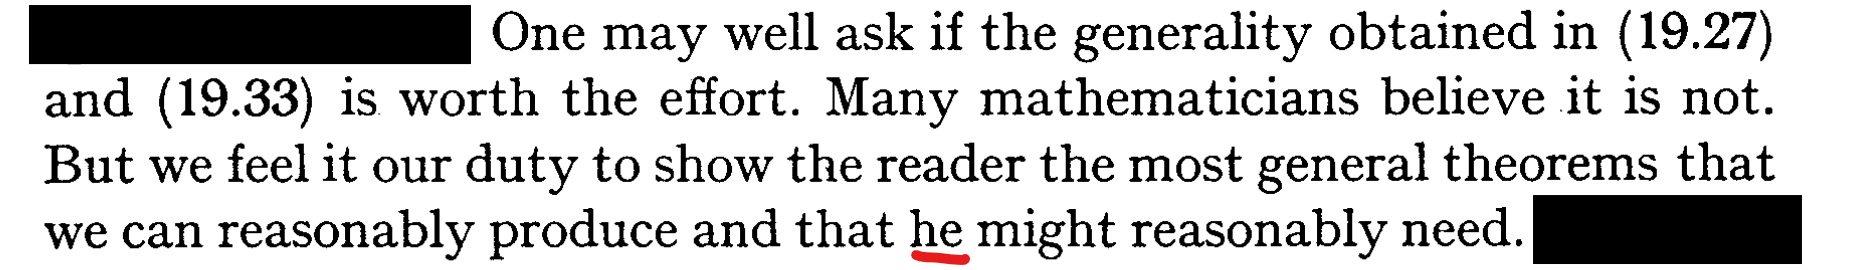
\includegraphics[scale=0.8]{A quote.png}\retTwo\par}

I'm not gonna lie, while going down research rabbitholes is really fun, I feel like Folland\\ really oversold the significance of this result. When I went into this rabbithole, I was under the impression from Folland that I'd be proving that if $\mu$ is an arbitrary Radon measure and $\nu \ll \mu$, then $\nu$ always has the form $f \df \mu$. But that is not what was proven in theorems 19.27 and 19.32 so I don't know what Folland was yappin about. Considering the lack of specific details that Folland gives, I can't help but suspect that Folland didn't entirely understand what Hewitt and Stromberg actually proved. Although, I don't necessarily blame Folland for that.\retTwo

Hewitt and Stromberg were difficult for me to understand partly because they had a lot of (in my opinion) very questionable conventions. For example, I tried my best to hide it away as much as possible but Hewitt and Stromberg explicitely treated every measure as the restriction of an outer measure to the $\sigma$-algebra of $\mu^*$-measurable sets rather than abstracting that away because I guess they always wanted their $\sigma$-algebras to be as large as possible. In fact, while I was skimming the book I even saw some other sections where they talked about extending their measures to even larger $\sigma$-algebras. Never mind that there are advantages to working on a smaller $\sigma$-algebra (see for instance page 55 of my journal: when working on a larger $\sigma$-algebra we lose that continuity implies measurability\dots).\newpage

I'll also mention that the choice of math font in their book is awful and I couldn't help but wonder if they knew what kerning is. Anyways I guess my review of their book is that it feels dated and very clunky. Although, maybe I only had a mixed experience because I'm not an intended reader. (cough cough)\retTwo

Anyways, while getting a milkshake with my apartment-mates, I thought of a few ideas for how to make the preceding theorems actually useful.\retTwo

\mySepTwo

My first challenge is that I'm primarily working with Borel Radon measures while Hewitt and Stromberg weren't. This leads me to the following result:\retTwo

\exTwo\ul{Proposition:} Suppose $X$ is an LCH space and let $\mu$ and $\nu$ be positive Radon measures on $(X, \mathcalli{B}_X)$ such that $\nu \ll \mu$. Then let $(X, \mathcal{M}_\mu, \overline{\mu})$ be the saturation of the completion of $(X, \mathcalli{B}_x, \mu)$ and let $(X, \mathcal{M}_\nu, \overline{\nu})$ be the saturation of the completion of $(X, \mathcalli{B}_x, \nu)$.
\begin{itemize}
	\item In general $\mathcal{M}_\mu \neq \mathcal{M}_\nu$.
	
	\begin{myIndent}\exThreeP
		Proof:\\
		Let $X = \mathbb{R}$. Then set $\mu$ to be the Lebesgue measure and set $\nu$ equal to the zero\\ measure (i.e. the measure for which every set is null). Note that we trivially have\\ that $\nu \ll \mu$. Also, both are easily seen to be Radon measures.\retTwo
		
		Since $\mu$ and $\nu$ are $\sigma$-finite, we know by the exercise on pages 158 and 159 that $\mathcal{M}_\mu$ and $\mathcal{M}_\nu$ are just the completions of $\mathcal{M}$ with respect to $\mu$ and $\nu$ respectively. Since $\nu(X) = 0$, we have that $\mathcal{M}_\nu = \mathcal{P}(X)$. Meanwhile, because of the existance of Vitali sets, we know that $\mathcal{M}_\mu \neq \mathcal{P}(X)$. $\blacksquare$.\retTwo
	\end{myIndent}

	\item We do always have that $\mathcal{M}_\mu \subseteq \mathcal{M}_\nu$ when $\mu$ and $\nu$ are Radon and $\nu \ll \mu$.
	
	\begin{myIndent}\exThreeP
		Proof: (I got this argument from Hewitt and Stromberg 19.33)\\
		Suppose $A \in \mathcal{M}_\mu$ and let $F \subseteq X$ be any compact set. Since $A$ is locally measurable with respect to the completion of $\mu$, we know that $A \cap F$ is in the completion of $\mathcalli{B}_X$ with respect to $\mu$. So let $A \cap F = E \cup N$ where $E \in \mathcalli{B}_X$ and $N \subseteq N^\prime$ with $N^\prime \in \mathcalli{B}_X$ and $\mu(N^\prime) = 0$. Then since $\mu(N^\prime) = 0$ implies that $\nu(N^\prime) = 0$, we know that $A \cap F$ is in the complection of $\mathcalli{B}_X$ with respect to $\nu$. By the lemma on page 161, this proves that $A \in \mathcal{M}_\nu$. $\blacksquare$\retTwo
	\end{myIndent}

	\item We do always have that $\overline{\nu}|_{\mathcal{M}_\mu} \ll \overline{\mu}$.
	
	\begin{myIndent}\exThreeP
		Proof:\\
		Suppose $A \in \mathcal{M}_\mu$ with $\overline{\mu}(A) = 0$. Since $A$ has finite measure, we know that $A$ is not merely locally measurable but also that $A$ is in the completion of $\mathcalli{B}_X$ with respect to $\mu$. Hence, there exists a set $N \in \mathcalli{B}_X$ such that $A \subseteq N$ and $\mu(N) = 0$. But now since $\nu \ll \mu$, we have that $\nu(N) = 0$. In turn, $\overline{\nu}(A) \leq \nu(N) = 0$. This proves that $\overline{\mu}(A) = 0 \Longrightarrow \overline{\nu}(A) = 0$.  $\blacksquare$\newpage
	\end{myIndent}
\end{itemize}

\hTwo It follows that if $X$ is an LCH space, then given any two positive Radon measures $\mu$ and $\nu$ on $(X, \mathcalli{B}_X)$ with $\nu \ll \mu$ we can extend $\mu$ and $\nu$ to measures $\overline{\mu}$ and $\overline{\nu}$ on a common $\sigma$-algebra $\mathcal{M}$ with precisely the following properties:\\ [-18pt]
\begin{itemize}
	\item $\overline{\mu}$ and $\overline{\nu}$ are both outer regular on all sets and inner regular on all $\sigma$-finite sets;\\ [-18pt]
	\item $\overline{\mu}$ and $\overline{\nu}$ are both finite on all compact sets;\\ [-18pt]
	\item $(X, \mathcal{M}, \overline{\mu})$ is the saturation of the completion of $(X, \mathcalli{B}_X, \mu)$;\\ [-18pt]
	\item $(X, \mathcal{M}, \overline{\mu})$ is decomposable;\\ [-18pt]
	\item $\overline{\nu} \ll \overline{\mu}$.\retTwo
\end{itemize}

Now using the theorems from Hewitt and Stromberg, I want to show that $\overline{\nu} = \overline{f} \df \overline{\mu}$ for some $\overline{\mu}$-measurable function $\overline{f}$. As it turns out, when $\nu$ is $\sigma$-finite (which in turn means $\overline{\nu}$ is $\sigma$-finite), this is always possible:\retTwo

\exTwo\mySepTwo

\ul{Proposition:} Let $(X, \mathcal{M})$ be a measurable LCH space and suppose $\mu$ and $\nu$ are positive measures on $(X, \mathcal{M})$ satisfying that $\nu$ is inner regular on all $\sigma$-finite sets; that $\mu$ is finite on all compact sets; that $\nu \ll \mu$; and that $(X, \mathcal{M}, \mu)$ is decomposable via the decomposition $\mathcalli{F}$. If $\nu$ is $\sigma$-finite, then there exists an $\mathcal{M}$-measurable function $f: X \to [0, \infty)$ which vanishes outside a set on which $\mu$ is $\sigma$-finite such that $\nu(A) = \int_A f \df \mu$ for all $A \in \mathcal{M}$. Furthermore, if $\nu$ is finite, then $f \in L^1(\mu)$. And if $g : X \to [0, \infty)$ is another function satisfying $\nu(A) = \int_A g \df \mu$ for all $A \in \mathcal{M}$, then $f = g$ $\mu$-a.e.

\begin{myIndent}\exThreeP
	Proof:\\
	We shall first suppose that $\nu$ is finite. Then by applying theorem 19.27 on page 156, we know there exists a measurable function $f: X \to [0, \infty)$ satisfying that $\nu(A) = \int_A f \df \mu$ whenever $\mu$ is $\sigma$-finite on $A$. Furthermore, since $\mu(F) < \infty$ for all $F \in \mathcalli{F}$, we thus know that $\nu(F) = \int_F f \df \mu$ for all $F \in \mathcalli{F}$.\retTwo

	Now recall that $\sum_{F \in \mathcalli{F}} \nu(F)$ is by definition equal to the suprememum of all finite sums of the $\nu(F)$. Thus, while we cannot currently guarentee strict equality due to the fact that $\mathcalli{F}$ may be uncountable, we can at least say that $\nu(X) \geq \sum_{F \in \mathcalli{F}}\nu(F)$. And since $\nu(X) < \infty$, this proves that there is a countable subset $\mathcalli{F}_1 \subseteq \mathcalli{F}$ satisfying that $\nu(F) = 0$ for all $F \notin \mathcalli{F}_1$. And clearly $\nu(X) = \nu(\hspace{-0.1em}\bigcup\limits_{F \notin \mathcalli{F}_1}\hspace{-0.1em} F) + \hspace{-0.1em}\sum\limits_{F \in \mathcalli{F}_1} \hspace{-0.1em}\nu(F)$.\retTwo

	Now we claim $\nu(\bigcup_{F \notin \mathcalli{F}_1} F) = 0$. After all, if the set weren't null, then we'd have that\\ $0 < \nu(\bigcup_{F \notin \mathcalli{F}_1} F) \subseteq \nu(X) < \infty$. It would thus follow by the inner regularity of $\nu$ that\\ there is a compact set $K \subseteq \bigcup_{F \notin \mathcalli{F}_1} F$ with $\nu(K) > 0$. But then we'd have that\\ $\mu(K) < \infty$, which means $\nu(K) = \int_K f \df \mu$ and $\mu(K) = \sum_{F \in \mathcalli{F}}\mu(F \cap K)$.\retTwo
	
	Now we can't have that $\mu(K) = 0$ since that contradicts that $\nu \ll \mu$. Hence, since $\mu$ is decomposable there's a nonempty countable family $\mathcalli{F}_2 \subseteq \mathcalli{F}$ such that $\mu(F \cap K) > 0$ for all $F \in \mathcalli{F}_2$ and $\mu(K) = \sum_{F \in \mathcalli{F}_2}\mu(F \cap K)$ (which in turn means $\mu(\bigcup_{F \notin \mathcalli{F}_2} F \cap K) = 0$). Also, since $K$ doesn't intercept any $F \in \mathcalli{F}_1$, we know that $\mathcalli{F}_1 \cap \mathcalli{F}_2 = \emptyset$. But now note that:
	
	{\centering$0 < \nu(K) = \int_K f \df \mu = \sum_{F \in \mathcalli{F}_2} \int_{F \cap K} f \df \mu = \sum_{F \in \mathcalli{F}_2} \nu(F \cap K)$.\newpage\par}

	This implies that there is some $F \in \mathcalli{F}_2$ such that $\nu(F) > \nu(F \cap K) > 0$. But that is a contradiction since we already know that $\nu(F) = 0$ if $F \notin \mathcalli{F}_1$. Hence, we have proven that there is a set $E = \bigcup_{F \in \mathcalli{F}_1} F$ which $\mu$ is $\sigma$-finite on such that $\nu(X) = \nu(E)$. And in turn, we've now proven that $\nu = f\chi_E \df \mu$.
	\begin{myIndent}\exPPP
		And as a side note: $f\chi_E \in L^1(\mu)$ because $\int f \chi_E \df \mu = \nu(X) < \infty$.\retTwo
	\end{myIndent}

	Next, we consider the case where $\nu$ is $\sigma$-finite. Let $(X_n)_{n \in \mathbb{N}}$ be a partition of $X$ consisting of finitely measurable sets. Then by identical reasoning as before, we can find for each $n$ a set $E_n \subseteq X$ on which $\mu$ is $\sigma$-finite and $\nu(X_n \cap A) = \int_A f \chi_{E_n} \df \mu$ for all $A \in \mathcal{M}$. Also, since $E_n \subseteq X_n$ for all $n$, it is clear that they are all disjoint. So, $E \coloneqq \bigcup_{n \in \mathbb{N}} E_n$ satisfies that $\mu$ is $\sigma$-finite on $E$ and $f\chi_E = \sum_{n \in \mathbb{N}} f\chi_{E_n}$. Also, it is clear that $\nu = f\chi_E \df \mu$ since:
	
	{\centering$\nu(A) = \sum_{n \in \mathbb{N}}\nu(X_n \cap A) = \sum_{n \in \mathbb{N}}\int_A f\chi_{E_n} \df \mu = \int_A f \chi_E \df \mu$ for all $A \in \mathcal{M}$.\retTwo\par}
	
	Finally, we show uniqueness. Suppose $g: X \to [0, \infty)$ is another function satisfying that $\nu = g \df \mu$ and let $B = \{x \in X: f(x)\chi_E(x) \neq g(x)\}$. Then it's clear that:
	
	{\centering$B = (B \cap E) \cup (B - E)$.\retTwo\par}
	
	Since $E$ is $\sigma$-finite, we already know from theorem 19.27 that there is a $\mu$-null set $N_1$ with $B \cap E \subseteq N_1$. Also, $B - E = \{x \in X - E : g(x) > 0\}$. So, if $\mu(B - E) > 0$, then we'd have that $\nu(B - E) = \int_{B - E} g \df \mu > 0$. But that contradicts that $\nu(X - E) = 0$. So, we can conclude that $\mu(B - E) = 0$. This proves that $f\chi_E = g$ $\mu$-a.e. $\blacksquare$\retTwo
\end{myIndent}

\mySepTwo

\hTwo To finish making this useful for our purposes we need to find a $\mathcalli{B}_X$-measurable function $f$ such that $\overline{f} = f$ $\overline{\mu}$-a.e. That way, for all $A \in \mathcalli{B}_X$ we have that:

{\centering $\int_A f \df \mu = \int_A f \df \overline{\mu} = \int_A \overline{f} \df \overline{\mu} = \overline{\nu}(A) = \nu(A)$ \retTwo\par}

Fortunately, if we let $(X, \mathcalli{N}, \overline{\mu}|_{\mathcalli{N}})$ be the completion of $(X, \mathcalli{B}_X, \mu)$ (meaning $(X, \mathcal{M}, \overline{\mu})$ is the saturation of $(X, \mathcalli{N}, \overline{\mu}|_{\mathcalli{N}})$), then we know  that $\overline{f}$ is $\mathcalli{N}$-measurable.

\begin{myIndent}\pracTwo
	Proof:\\
	We know $\overline{f}$ vanishes outside a set on which $\overline{\mu}$ is $\sigma$-finite. It follows that if $a < 0$, then $\overline{f}^{-1}((a, \infty)) = X \in \mathcalli{N}$; and if $a \geq 0$, then $\overline{f}^{-1}((a, \infty))$ is $\sigma$-finite. Now we claim that all sets for which $\overline{\mu}$ is $\sigma$-finite are in $\mathcalli{N}$. After all, if $\overline{\mu}$ is $\sigma$-finite on $E$, then we know there is a sequence of sets $(E_n)_{n \in \mathbb{N}}$ whose union is $E$ and which satisfy that $\overline{\mu}(E_n) < \infty$ for all $n$. Then since all the $E_n$ have finite measure, we know that $E_n \in \mathcalli{N}$ for all $n$. So, $E$ is also in $\mathcalli{N}$.\retTwo

	With that, we've shown that $\overline{f}^{-1}((a, \infty))$ is $\mathcalli{N}$-measurable for all $a \in \mathbb{R}$. This proves that $\overline{f}$ is $\mathcalli{N}$-measurable. $\blacksquare$\retTwo
\end{myIndent}

Now, it is a simple application of the proposition on page 46 of my latex math 240a notes to show there exists a $\mathcalli{B}_X$-measurable function $f$ such that $\overline{f} = f$ a.e. with respect to $(X, \mathcalli{N}, \overline{\mu}|_{N_x})$. And since saturating the latter $\sigma$-algebra doesn't add any new null sets, we have that $f = \overline{f}$ $\overline{\mu}$-a.e. Thus, we have found a $\mathcalli{B}_X$-measurable function $f$ such that\\ $\nu = f \df \mu$.\newpage

One more note I want to make is that if $g$ is another $\mathcalli{B}_X$-measurable function such that $\nu = g \df \mu$, then $f = g$ $\mu$-a.e.

\begin{myIndent}\pracTwo
	Proof:\\
	Since $\overline{f}$ vanishes outside a set on which $\overline{\mu}$ is $\sigma$-finite and $\overline{f} = f$ $\overline{\mu}$-a.e., we also know that $f$ vanishes outside a set on which $\overline{\mu}$ is $\sigma$-finite. If we call that set $E$, then we have that $f = f\chi_E$ everywhere. Also note that since $E$ is in $\mathcalli{N}$ on account of $\overline{\mu}$ being $\sigma$-finite on it, we can expand $E$ to a larger set in $\mathcalli{B}_X$ that $\overline{\mu}$ is still $\sigma$-finite on. Hence, we may without loss of generality just say that $E \in \mathcalli{B}_X$. One final note is that if $\overline{\mu}$ is $\sigma$-finite on $E$, then we also know that $\mu$ is $\sigma$-finite on $E$. So, we conclude that $f = f\chi_E$ where $E \in \mathcalli{B}_X$ and $\mu$ is $\sigma$-finite on $E$.\retTwo

	Now let $B \coloneqq \{x \in X: g(x) \neq f(x)\}$. Then we know that $B = (B \cap E) \cup (B - E)$. Our claim is that both of the latter sets are null with respect to $\mu$.
	\begin{myIndent}
		First suppose that $\mu(B - E) > 0$. Then since $B - E = \{x \in X - E : g(x) > 0\}$, we'd have to have that $\nu(B - E) = \int_{B - E} g \df \mu > 0$. But that contradicts that $\nu(B - E) = \int_{B - E} f \df \mu = \int_{B - E} 0 \df \mu = 0$. So, we conclude that $\mu(B - E) = 0$.\retTwo

		Meanwhile, if $B \cap E$ is not a null set, then because $\mu$ is $\sigma$-finite (and thus also\\ semifinite) on $E$, we must be able to pick a set $C \in \mathcalli{B}_X$ such that $0 < \mu(C) < \infty$\\ and $g(x) \neq f(x)$ for all $x \in C$. Then in turn we'd have that:

		{\centering $\int_C |f(x) - g(x)| \df \mu> 0$ \retTwo\par}

		But note that since $\nu$ is $\sigma$-finite, we know there there is a disjoint sequence of\\ sets $\{C_n\}_{n \in \mathbb{N}}$ such that $C = \bigcup_{n \in \mathbb{N}} C_n$ and $\nu(C_n) = \int_{C_n}f \df \mu = \int_{C_n} g \df \mu < \infty$\\ for all $n$. Also, for each $n$ we can define $C_n^+ \coloneqq \{x \in C_n : f(x) > g(x)\}$ and\\ $C_n^- \coloneqq \{x \in C_n : g(x) > f(x)\}$. And thus:
		
		{\center $\int_C |f(x) - g(x)| \df \mu = \sum\limits_{n \in \mathbb{N}} \int_{C_n^+}(f(x) - g(x))\df \mu + \sum\limits_{n \in \mathbb{N}} \int_{C_n^-}(g(x) - f(x))\df \mu$ \retTwo\par}

		But now because $\int_{C_n^\pm} f(x) \df \mu = \int_{C_n^\pm} g(x) \df \mu = \nu(C_n^\pm)$ where $\nu(C_n^\pm)$ is finite, we must have that $\int_C |f(x) - g(x)| \df \mu = 0$ as:
		
		{\center $\int_{C_n^+} (f(x) - g(x)) \df \mu = 0 = \int_{C_n^-} (g(x) - f(x))\df \mu$ for all $n$.\retTwo\par}

		This is a contradiction. So, we've proven that $\mu(B \cap E) = 0$. $\blacksquare$\retTwo
	\end{myIndent}
\end{myIndent}

So to sum all my previous work up, we have the following result:\retTwo

\exTwo\ul{A Third Extension of the Lebesgue-Radon-Nikodym Theorem:}
\begin{myIndent}
	If $X$ is an LCH space and $\mu$ and $\nu$ are positive Radon measures on $(X, \mathcalli{B}_X)$ such that\\ $\nu$ is $\sigma$-finite and $\nu \ll \mu$, then there exists a measurable function $f: X \to [0, \infty)$\\ which vanishes outside of a set where $\mu$ is $\sigma$-finite and which satisfies that $\nu = f \df \mu$.\\ Furthermore, if $g$ is another measurable function satisfying that $\nu = g \df \mu$, then\\ $f = g$ $\mu$-a.e.\retTwo
\end{myIndent}

\hTwo Also, we can clearly extend this theorem to the case where $\nu$ is signed by just applying the theorem to the positive and negative variations separately of $\nu$. And in order to prove uniqueness in this case we can employ a similar strategy as was shown at the top of page 158.\newpage

Going a step further, if $\nu$ is complex, then we can apply the prior reasoning to the real and imaginary variations of $\nu$. Thus, we get the most general result that I will attempt to prove:\retTwo

\exTwo\ul{A Fourth Extension of the Lebesgue-Radon-Nikodym Theorem:}
\begin{myIndent}
	Suppose $X$ is an LCH space and $\mu$ is a Radon measure on $(X, \mathcalli{B}_X)$. If $\nu$ is a complex\\ or $\sigma$-finite signed Radon measure with $\nu \ll \mu$, then there exists a measurable\\ function $f: X \to \mathbb{R}$ (or $\mathbb{C}$) which vanishes outside of a set where $\mu$ is $\sigma$-finite and which satisfies that $\nu = f \df \mu$. Furthermore, if $g$ is another measurable function satisfying that $\nu = g \df \mu$, then $f = g$ $\mu$-a.e.\retTwo
\end{myIndent}

\hTwo I will note that this is still not as general of a statement as Folland was claiming Hewitt and Stromberg were making. Yet it is enough for a specific claim which Folland makes and I will take notes on tomorrow to be true. Anyways, it's been four days since I started going down this rabbithole and I need to grade.

\mySepTwo

\hOne\dispDate{8/30/2025}

\hTwo Let $X$ be an LCH space. Given any fixed positive Radon measure $\mu$, we can isometrically embed $L^1(\mu)$ into $M(X)$ as follows:

\begin{myIndent}\hThree
	Define a map $L^1(\mu) \hookrightarrow M(X)$ such that $f \mapsto f \df \mu$ for all $f \in L^1(\mu)$. By the exercise on page 154, we know that $f \df \mu$ is in fact Radon. Also, we know that the image of this map is precisely the subset of $M(X)$ consisting of all complex measures that are absolutely continuous with respect to $\mu$ (this works even if $\mu$ is not Radon by the rabbithole I went down this past week).\retTwo

	Also, we can easily see that $\| f \df \mu \|_{M(X)} = \|f\|_1$.
	\begin{myIndent}\pracTwo
		I want to be slightly careful about saying this since I'm not assuming $\mu$ is $\sigma$-finite.\retTwo

		Let $\nu = f \df \mu$. Now we know from math 240a that there exists a measurable function\\ [2pt] $g$ with $|g| = 1$ $|\nu|$-a.e. such that $\nu = g \df |\nu|$. Furthermore, we know from the rabbit\\ [2pt] hole before that there exists a nonnegative function $\frac{\df |\nu|}{\df \mu}$ such that $\df |\nu| = \frac{\df |\nu|}{\df \mu} \df \mu$. Hence, we have that $\nu = g \frac{\df |\nu|}{\df \mu} \df \mu$, and this proves that $f = g \frac{\df |\nu|}{\df \mu}$ a.e.. Then in turn we also have that $|f| = \frac{\df |\nu|}{\df \mu}$ and $|\nu| = |f|\df \mu$. This proves that even if $\mu$ is not\\ $\sigma$-finite, we still have that $\nu = f \df \mu \Longrightarrow |\nu| = |f|\df\mu$.\retTwo
	\end{myIndent}
\end{myIndent}

An important application of the above fact is that if $m$ is the Lebesgue measure on $\mathbb{R}^n$, then we can identify $L^1(m)$ as a subspace $M(\mathbb{R}^n)$. This will be used in my journal later.\retTwo

Given a net $\langle \mu_\alpha \rangle_{\alpha \in A}$ and another measure $\mu$ in $M(X)$, we have that $\mu_\alpha \to \mu$ in the \weakst topology on $M(X) = C_0(X)^*$ iff we have that $\int f \df \mu_\alpha \to \int f \df \mu$ for all $f \in C_0(X)$. This topology is important enough to be given a second name: the \udefine{vague topology} on $M(X)$.\newpage

Before covering the next theorem in Folland, I'm gonna do another side quest concerning the Stone-Weierstrass Theorem.\retTwo

\Hstatement\blab{Exercise 4.67:} Let $X$ be a noncompact LCH space. If $\mathcalli{A}$ is a closed subalgebra of $C_0(X, \mathbb{R})$ that separates points, then either $\mathcalli{A} = C_0(X, \mathbb{R})$ or $\mathcalli{A} = \{f \in C_0(X, \mathbb{R}) : f(x_0) = 0\}$ for some $x_0 \in X$.

\begin{myIndent}\HexOne
	Proof:\\
	First suppose there does not exist any $x_0 \in X$ such that $f(x_0) = 0$ for all $f \in \mathcalli{A}$. Then let $Y$ be the Alexandroff (i.e. one-point) compactification of $X$ and $i: C_0(X, \mathbb{R}) \hookrightarrow C(Y, \mathbb{R})$ be the injective map that continuously extends each $f$ to $Y$ by setting $f(\infty) = 0$. Now $i(\mathcalli{A})$ is a subalgebra of $C(Y, \mathbb{R})$ that separates points and for which $x_0 \coloneqq \infty$ satisfies that $f(x_0) = 0$ for all $f \in i(\mathcalli{A})$. So by the Stone Weierstrass theorem we already proved, we know that:\\ [-16pt]

	{\centering $\overline{i(\mathcalli{A})} = \{f \in C(Y, \mathbb{R}) : f(\infty) = 0\}$ \retTwo\par}
	
	But now we claim that $i(\mathcalli{A})$ is closed. For suppose $g \in \overline{i(\mathcalli{A})}$ and  $\{f_n\}_{n \in \mathbb{N}}$ is a sequence in $i(\mathcalli{A})$ converging uniformly to $g$. Then it's clear that $f_n|_X \to g|_X$ uniformly. So $g|_X \in \mathcalli{A}$ since $\mathcalli{A}$ is closed. And in turn $g \in i(\mathcalli{A})$.\retTwo
	
	This shows that $i(\mathcalli{A}) = \overline{i(\mathcalli{A})} = \{f \in C(Y, \mathbb{R}) : f(\infty) = 0\}$. It then follows that\\ $\mathcalli{A} = C_0(X, \mathbb{R})$.\retTwo

	Next suppose there does exist some $x_0 \in X$ such that $f(x_0) = 0$ for all $f \in \mathcalli{A}$. This poses a problem to our previous approach because $i(\mathcalli{A})$ no longer separates points. So to get around this, we first consider the subspace $X^\prime = X - \{x_0\}$. Importantly, $X^\prime$ is still Hausdorff. Also, since $X^\prime$ is an open subset of $X$, we know any $x \in X^\prime$ has a compact neighborhood $N \subseteq X^\prime$. Hence, $X^\prime$ is locally compact.\retTwo

	Next, let $j$ be the map restricting the domain of each $f \in C_0(X, \mathbb{R})$ to $X^\prime$. Then note that\\ [1pt] if $f(x_0) = 0$, then $f|_{X^\prime} \in C_0(X^\prime, \mathbb{R})$. After all, if $\{x \in X : f(x) > \varepsilon\}$ is compact and\\ [1pt] entirely contained in $X^\prime$, then we also know that $\{x \in X^\prime : f|_X(x) > \varepsilon\}$ is compact in\\ [1pt] the subspace topology of $X^\prime$. As a result of this, we know that $j$ is an injective map from\\ [1pt] $\{f \in C_0(X, \mathbb{R}) : f(x_0) = 0\}$ into $C_0(X^\prime, \mathbb{R})$.\retTwo

	Now, it is easily seen that $j(\mathcalli{A})$ is an algebra that separates points and vanishes nowhere. And, it is also seen similarly to earlier that $j(\mathcalli{A})$ is closed. But then by the first case\\ we proved in this exercise, we know that $j(\mathcalli{A}) = C_0(X^\prime, \mathbb{R})$. Hence, it follows that\\ $\mathcalli{A} = \{f \in C_0(X, \mathbb{R}) : f(x_0) = 0\}$. $\blacksquare$\retTwo
\end{myIndent}

\hTwo Now in the next theorem, Folland brought up this exercise because he needs it to prove that $C^1_c(\mathbb{R})$ is dense in $C_0(\mathbb{R})$. However, in my math 240c notes I already proved a stronger statement that $C^\infty_c(\mathbb{R})$ is dense in $C_0(\mathbb{R})$. So was proving this unnecessary? No comment.\retTwo

\exTwo\hypertarget{Folland Proposition 7.19}{\ul{Proposition 7.19:}} Suppose $\mu, \mu_1, \mu_2, \ldots \in M(\mathbb{R})$ and let $F_n(x) = \mu_n((-\infty, x])$ and\\ $F(x) = \mu((-\infty, x])$.\\ [-22pt]
\begin{itemize}
	\item[(a)] If $\sup_{n \in \mathbb{N}}\|\mu_n\| < \infty$ and $F_n(x) \to F(x)$ for every $x$ at which $F$ is continuous, then $\mu_n \to \mu$ vaguely.\newpage
	
	\begin{myIndent}\exThreeP
		Proof:\\
		By Folland theorem 3.29 (check my paper math 240a notes), we know $F$ and each of the $F_n$ are all in \NBV. In turn, this means that $F$ and all the $F_n$ are continuous except at countably many points. So, our assumed conditions actually guarentee that $F_n \to F$ a.e. with respect to the Lebesgue measure.\retTwo

		Now consider any $f \in C^1_c(\mathbb{R})$. By applying theorem 3.36 from math 240a, we can say that $\int f \df \mu = -\int f^\prime F \df x$ and that $\int f \df \mu_n = -\int f^\prime F_n \df x$ for all $n$.
		\begin{myIndent}\exPPP
			Side note: I just realized why theorem 3.36 is a strict generalization of\\ integration by parts as taught in undergrad analysis. If $f$ is a $C^1$ function\\ on $[a, b]$, then we know $f$ is absolutely continuous on $[a, b]$ via the mean\\ value theorem. And it follows then that the measure $f^\prime \df t$ satisfies that\\ $f(x) - f(a) = \int_{(a, x]}f^\prime(t)\df t$ for all $x \in [a, b]$.\retTwo
			
			Next suppose $f$ is $C^1$ everywhere,  $f^\prime \in L^1(\mathbb{R})$, and $f(-\infty) = 0$. Then\\ by taking $a \to -\infty$ and $b \to +\infty$ in the last paragraph, we get that $f^\prime \df t$\\ is a measure satisfying that $f(x) = \int_{(-\infty, x]} f^\prime \df t$.\retTwo

			Thus, so long as $f$ is $C^1$, $f(-\infty) = 0$, and $f^\prime \in L^1$, we know that $f^\prime \df t$\\ is the unique borel measure such that $f(x) = \int_{(-\infty, x]} f^\prime \df t$. And since $f$ is continuous, we can always apply theorem 3.36 to $f$ and any other {\NBV} function.
			\begin{myIndent}\pracTwo
				Now if only I had thought about that while I was actually taking math 240. This is why I failed the qual. AAUGH.\retTwo
			\end{myIndent}
		\end{myIndent}

		But note that $\|F_n\|_u \leq \|\mu_n\|$ for all $n$. So if we set $C = \|f^\prime\|_u \sup_{n \in \mathbb{N}}\|\mu_n\|$, then we can apply dominated convergence theorem using an upper bound of $C\chi_{\supp(f^\prime)}$ to show that $-\int f^\prime F_n \df x \to -\int f^\prime F \df x$ as $n \to \infty$. Hence, $\int f \df \mu_n \to \int f \df \mu$ as $n \to \infty$.\retTwo

		Consequently, we have shown that $\int f \df \mu_n \to \int f \df \mu$ on a dense subset of $C_0(\mathbb{R})$. And so, by proposition 5.17 (see math 240b notes), we know $\int f \df \mu_n \to \int \df \mu$ for all $f \in C_0(\mathbb{R})$. This proves that $\mu_n \to \mu$ vaguely. $\blacksquare$\retTwo
	\end{myIndent}

	\item[(b)] If $\mu_n \to \mu$ vaguely, then $\sup_{n \in \mathbb{N}} \|\mu_n\| < \infty$. If in addition the $\mu_n$ are positive, then $F_n(x) \to F(x)$ at every $x$ at which $F$ is continuous. 

	\begin{myIndent}\exThreeP
		Proof:\\
		By the Riesz Representation theore, we already know that the linear functional\\ $f \mapsto \int f \df \mu_n$ from $C_0(\mathbb{R})$ to $\mathbb{C}$ has the operator norm $\|\mu_n\|$. Also, since $\mu_n \to \mu$\\ vaguely, we know that $\sup_{n \in \mathbb{N}}|\int f \df \mu_n| < \infty$ for all $f \in C_0(\mathbb{R})$. Thus by the uniform\\ boundedness principle, we know that $\sup_{n \in \mathbb{N}}\|\mu_n\| < \infty$.\retTwo

		Next suppose all the $\mu_n$ are positive. Then since $\mu_n \to \mu$ vaguely, we claim that $\mu$ is positive.
		\begin{myIndent}\exPPP
			Note: The following the reasoning works on any general LCH space $X$.\newpage 

			Write $\mu = \mu^{(1)} - \mu^{(2)} + i(\mu^{(3)} - \mu^{(4)})$ where the four latter measures are\\ positive Radon measures. Since $\int f \df \mu_n \to \int f \df \mu$ for all $f \in C_0(X)$ and all the $\mu_n$ are positive, we know that if $f$ is nonnegative and real, then $\int f \df \mu \geq 0$. This is enough to show that $\mu^{(i)} = 0$ unless $i = 1$.\retTwo

			Suppose for the sake of contradiction that $\mu^{(2)} = \alpha > 0$ on some set\\ $A \in \mathcalli{B}_X$. Then by restricting our set $A$ using a Hahn decomposition, we can also say without loss of generality that $\mu^{(1)}(A) = 0$. But now pick any $\varepsilon \in (0, \frac{\alpha}{2})$. By the outer regularity of $\mu^{(1)}$ we know there exists an open set $U \supseteq A$ such that $\mu^{(1)}(U) < \varepsilon$. At the same time, by the inner regularity of $\mu^{(2)}$ we know there exists a compact set $K \subseteq A$ such that $\mu^{(2)}(K) > \alpha - \varepsilon$. And by Urysohn's lemma, we know there is a function $\phi \in C_c(X, [0, 1])$ such that $\phi(K) = \{1\}$ and $\supp(\phi) \subseteq U$. It now follows that:
			
			{\centering\begin{tabular}{l}
				$\rea{\int \phi \df \mu} = \int \phi \df \mu^{(1)} - \int \phi \df \mu^{(2)}$\\
				$\phantom{\rea{\int \phi \df \mu}} \leq \int \chi_U \df \mu^{(1)} - \int \chi_K \df \mu^{(2)} < \varepsilon - (\alpha - \varepsilon) < 0$.
			\end{tabular}\retTwo\par}

			But that contradicts our earlier statement that $\int \phi \df \mu$ is real and nonnegative if $\phi$ is real and nonnegative. So, we conclude no such $A$ exists.\retTwo

			Similar reasoning shows that $\mu^{(3)}$ and $\mu^{(4)}$ are zero.\retTwo
		\end{myIndent}

		Now given any $a$ at which $F$ is continuous, choose any $\varepsilon > 0$ and $N$ such that\\ $-N < a - 2\varepsilon$. Then letting $f \in C_c(\mathbb{R})$ be the function that is $1$ on $[-N, a]$,\\ $0$ on $(-\infty, -N - \varepsilon) \cup (a + \varepsilon, \infty)$, we have that:

		{\centering\begin{tabular}{l}
			$F_n(a) - F_n(-N) = \mu_n((-N, a])$\\ [4pt]
			$\phantom{F_n(a) - F_n(-N)} \leq \int f \df \mu_n \to \int f \df \mu \leq F(a + \varepsilon) - F(-N - \varepsilon)$.
		\end{tabular}\retTwo\par}

		And by taking $N \to \infty$ we thus get that $\limsup_{n \to \infty} F_n(a) \leq F(a + \varepsilon)$.\retTwo

		Meanwhile, letting $g \in C_c(\mathbb{R})$ be the function that is $1$ on $[-N + \varepsilon, a - \varepsilon]$, $0$\\ on $(-\infty, -N] \cup [a, \infty]$, and linear in between, we have that:

		{\centering\begin{tabular}{l}
			$F_n(a) - F_n(-N) = \mu_n((-N, a))$\\ [4pt]
			$\phantom{F_n(a) - F_n(-N)} \geq \int g \df \mu_n \to \int g \df \mu \geq F(a - \varepsilon) - F(-N + \varepsilon)$.
		\end{tabular}\retTwo\par}

		And by taking $N \to \infty$ we thus get that $\liminf_{n \in \infty} F_n(a) \geq F(a - \varepsilon)$.\retTwo

		Now by taking $\varepsilon \to 0$ and using the fact that $F$ is continuous at $a$, we prove that $F_n(a) \to F(a)$ as $n \to \infty$. $\blacksquare$\retTwo
	\end{myIndent}
\end{itemize}

\dispDate{9/1/2025}

\hOne Today I want to clean up my knowledge about product measures by doing some exercises from Folland that I never got around to while I was taking math 240.\newpage

\Hstatement\blab{Exercise 2.11:} If $f : \mathbb{R} \times \mathbb{R}^k \to \mathbb{C}$ satisfies that $f(x, \cdot)$ is measurable on $\mathbb{R}^k$ for all $x \in \mathbb{R}$ and that $f(\cdot, y)$ is continuous on $\mathbb{R}$ for all $y \in \mathbb{R}^k$, then $f$ is Borel measurable on $\mathbb{R} \times \mathbb{R}^k$.

\begin{myIndent}\HexOne
	Proof:\\
	Let $n$ be any positive integer and for all $i \in \mathbb{Z}$, define $a_{i} = \sfrac{i}{n}$. Then define a function $f_n$ on $\mathbb{R} \times \mathbb{R}^k$ by setting for all $y \in \mathbb{R}^k$ and $x \in [a_{i}, a_{i+1}]$:

	\[f_n(x, y) = \frac{f(a_{i+1}, y)(x - a_{i}) - f(a_{i}, y)(x - a_{i+1})}{a_{i+1} - a_{i}}\]

	\phantom{.}\\

	In order to show that each $f_n$ is well defined, note that if $x = a_{i}$ for some $i \in \mathbb{Z}$, then:
	
	{\center$\frac{f(a_{i}, y)(x - a_{i-1}) - f(a_{i-1}, y)(x - a_{i})}{a_{i} - a_{i-1}} = f(a_{i}, y) = \frac{f(a_{i+1}, y)(x - a_{i}) - f(a_{i}, y)(x - a_{i+1})}{a_{i+1} - a_{i}}$\retTwo\par}

	\begin{myTindent}\HexPPP
		You may note that $f_n$ is essentially linearly interpolating because the\\ differents sets $\{a_i\} \times \mathbb{R}^k$ of the domain. And as $n \to \infty$ we are sampling more often.\retTwo
	\end{myTindent}

	We also claim that $f_n$ is measurable. After all, if $E \in \mathcal{M}$, then:

	{\centering $f_n^{-1}(E) = \bigcup_{i \in \mathbb{Z}} (f_n^{-1}(E) \cap ([a_i, a_{i+1}] \times \mathbb{R}^k))$ \retTwo\par}

	But now we know that $f_n$ is measurable on the domain $[a_i, a_{i+1}] \times \mathbb{R}^k$ since it is equal to a sum of products of measurable functions. $g(x, y) \coloneqq f(a_{i+1}, y)$ is measurable as a function from $\mathbb{R} \times \mathbb{R}^k$ because the projection map $(x, y) \mapsto (a_i, y)$ is a continuous map from $\mathbb{R} \times \mathbb{R}^k$ to $\mathbb{R}^k$ and we already assumed that $f(a_i, \cdot)$ is measurable on $\mathbb{R}^k$. Similarly, we can show that $h(x, y) \coloneqq f(a_i, y)$ is measurable. And since $(x - a_i)$ and $(x - a_{i+1})$ are continuous, we also know those parts of the expression for $f_n$ are measurable. And since $[a_i, a_{i+1}] \times \mathbb{R}^k$ is in $\mathcalli{B}_\mathbb{R} \otimes \mathcalli{B}_{\mathbb{R}^k}$ for each $i$, we can now conclude $f_n$ is measurable on its entire domain.\retTwo

	Now in order to show that $f$ is measurable, we claim that $f_n \to f$ pointwise. To prove this, consider any $x \in \mathbb{R}$ and $y \in \mathbb{R}^k$ and let $\varepsilon > 0$. Since $f(\cdot, y)$ is continuous, we know that there exists $\delta > 0$ such that $|f(x^\prime, y) - f(x, y)| < \varepsilon$ for all $x^\prime$ satisfying that $|x^\prime - x| < \delta$. Now suppose $n$ is large enough so that $\sfrac{1}{n} < \sfrac{\delta}{3}$. Then we know there exists $i \in \mathbb{Z}$ such that $x - \delta < a_i \leq x \leq a_{i+1} < x + \delta$. And in turn:

	{\center\begin{tabular}{l}
	$|f_n(x, y) - f(x, y)| = \left|\frac{f(a_{i+1}, y)(x-a_i) - f(a_i, y)(x-a_{i+1})}{a_{i+1} - a_i} - f(x, y)\right|$\\ [14pt]
	$\phantom{|f_n(x, y) - f(x, y)|} = \left|\frac{f(a_{i+1}, y)(x-a_i) - f(a_i, y)(x-a_{i+1})}{a_{i+1} - a_i} - f(x, y)\frac{(x - a_i) - (x - a_{i+1})}{a_{i+1} - a_i}\right|$\\ [14pt]
	$\phantom{|f_n(x, y) - f(x, y)|} = \left|\frac{(f(a_{i+1}, y) - f(x, y))(x-a_i)}{a_{i+1} - a_i} - \frac{(f(a_i, y) - f(x, y))(x-a_{i+1})}{a_{i+1} - a_i}\right|$\\ [14pt]
	$\phantom{|f_n(x, y) - f(x, y)|} = |f(a_{i+1}, y) - f(x, y)||\frac{(x-a_i)}{a_{i+1} - a_i}| + |f(a_i, y) - f(x, y)||\frac{(x-a_{i+1})}{a_{i+1} - a_i}|$\\ [14pt]
	$\phantom{|f_n(x, y) - f(x, y)|} \leq |f(a_{i+1}, y) - f(x, y)|\cdot 1 + |f(a_i, y) - f(x, y)|\cdot 1$\\ [14pt]
	$\phantom{|f_n(x, y) - f(x, y)|} < \varepsilon + \varepsilon = 2\varepsilon$. $\blacksquare$
	\end{tabular}\newpage\par}
\end{myIndent}

As a corollary, if $f: \mathbb{R}^n \to \mathbb{C}$ is continuous in each variable separately, then $f$ is measurable.

\begin{myIndent}\HexOne
	Proof:\\
	Suppose we already proved that if $g: \mathbb{R}^{n-1} \to \mathbb{C}$ is continuous in each variable, then $g$ is Borel measurable. Then consider $f$ as a function from $\mathbb{R} \times \mathbb{R}^{n-1}$ to $\mathbb{C}$. We know by our assumption that $f(\cdot, y)$ is continuous for all $y \in \mathbb{R}^{n-1}$. Also, we know by our inductive hypothesis that $f(x, \cdot)$ is measurable for all $x \in \mathbb{R}$. So by the reasoning in the last exercise, we have that $f$ is Borel measurable on $\mathbb{R} \times \mathbb{R}^{n-1}$.\retTwo
	
	And since $\mathcalli{B}_{\mathbb{R} \times \mathbb{R}^{n-1}} = \mathcalli{B}_{\mathbb{R}^n}$ when identifying $\mathbb{R} \times \mathbb{R}^{n-1}$ with $\mathbb{R}^n$, we've shown that $f$ is measurable. $\blacksquare$
	\begin{myTindent}\myComment\fontsize{11}{13}\selectfont
		I realize I still have not yet properly convinced myself of why\\ $\mathcalli{B}_{\mathbb{R} \times \mathbb{R}^{n-1}} \cong \mathcalli{B}_{\mathbb{R}^n}$. So, I'd like to set that and a few other conerns about products of measures straight tomorrow. But for now I need to study for physics.\retTwo
	\end{myTindent}
\end{myIndent}

\pracOne One more note I'd like to make is that this exercise is significant because we don't generally have that $f: \mathbb{R}^n \to \mathbb{C}$ being continuous with respect to each variable separately implies that $f$ is continuous. So essentially this exercise gives a strictly weaker sufficient condition for $f: \mathbb{R}^n \to \mathbb{C}$ to be Borel measurable than strict continuity. Also, this new condition is way easier to show.\retTwo

\dispDate{9/2/2025}

\hypertarget{Folland Exercise 2.45}{\Hstatement\blab{Exercise 2.45:}} Let $n \geq 3$ and suppose $(X_j, \mathcal{M}_j, \mu_j)$ is a measure space for $j = 1, \ldots, n$, and let us identify $\prod_{j=1}^n X_j$ with $(\prod_{j=1}^{n-1} X_j) \times X_n$  and $X_1 \times (\prod_{j=2}^{n} X_j)$ in the obvious ways.
\begin{itemize}
	\item We have that $\bigotimes_{j=1}^n \mathcal{M}_j = (\bigotimes_{j=1}^{n-1} \mathcal{M}_j) \otimes \mathcal{M}_n$.
	\begin{myIndent}\HexOne 
		Proof:\\ 
		For $i = 1, \ldots, n$ let $\pi_i$ be the projection of $\prod_{j=1}^n X_j$ onto $X_i$. Also let $\pi_{\widehat{n}}$ be the\\ projection of $\prod_{j=1}^n X_j$ onto $\prod_{j=1}^{n-1} X_j$ and for $k=1,\ldots,n-1$ let $\tau_{k}$ be the projection\\ of $\prod_{j=1}^{n-1} X_j$ onto $X_k$.\retTwo

		We know by definition that $\bigotimes_{j=1}^{n} \mathcal{M}_j$ is generated by the collection of sets:

		{\centering $A_1 \coloneqq \{\pi_j^{-1}(E) : j=1,\ldots,n \text{ and } E \in \mathcal{M}_j\}$.\retTwo\par}
		
		Meanwhile, by the proposition at the top of page 13 of my latex math 240a notes,\\ since $\{\tau_k^{-1}(E) : k=1,\ldots,n-1 \text{ and } E \in \mathcal{M}_k\}$ is a base for $\bigotimes_{j=1}^{n-1} \mathcal{M}_j$, we have that $(\bigotimes_{j=1}^{n-1} \mathcal{M}_j) \otimes \mathcal{M}_3$ is generated by the collection of sets:
		
		{\centering $A_2 \coloneqq \{\pi_{\widehat{n}}^{-1}(\tau^{-1}_k(E)) : k=1,\ldots,{n-1} \text{ and } E \in \mathcal{M}_k\} \cup \{\pi_n^{-1}(E) : E \in \mathcal{M}_3\}$.\retTwo\par}

		But now if $E \in \mathcal{M}_1$, we know that:
		
		{\centering$\pi^{-1}_{\widehat{n}}(\tau^{-1}_1(E)) = \pi^{-1}_{\widehat{n}}(E \times X_2 \times \cdots \times X_{n-1}) = E \times X_2 \times \cdots \times X_{n-1} \times X_n$.\retTwo\par}
		
		Repeating this reasoning for all $2 \leq k \leq n-1$ we can in fact see that $A_1 = A_2$. This shows that both of the sigma algebras in the problem are equal.\newpage
	\end{myIndent}

	\item By nearly identical reasoning, we have that $\bigotimes_{j=1}^n \mathcal{M}_j = \mathcal{M}_1 \otimes (\bigotimes_{j=2}^{n} \mathcal{M}_j)$. And note that this is enough to show that the $\bigotimes$ operation is associative and we get the same result no matter how we use parentheses to group together the $\mathcal{M}_j$ (see the top of page 113 of my math journal).\retTwo

	\item If all the $\mu_j$ are $\sigma$-finite, then $\mu_1 \times \cdots \times \mu_n = (\mu_1 \times \cdots \times \mu_{n-1}) \times \mu_n$.
	\begin{myIndent}\HexOne 
		Proof:\\ 
		If all the $\mu_j$ are $\sigma$-finite, then we know that $\mu_1 \times \cdots \times \mu_n$ is the unique measure\\ on $\bigotimes_{j=1}^n \mathcal{M}_j$ satisfying that for any rectangle $E_1 \times \cdots \times E_n$ where $E_k \in \mathcal{M}_k$ for\\ all $k=1,\ldots,n$:

		{\centering $\mu_1 \times \cdots \times \mu_n(E_1 \times \cdots \times E_n) = \mu_1(E_1)\cdots\mu_n(E_n)$ \retTwo\par}

		Meanwhile, we also have that $\mu_1 \times \cdots \times \mu_{n-1}$ is a measure on $\bigotimes_{j=1}^{n-1} \mathcal{M}_j$ satisfying that if $E_k \in \mathcal{M}_k$ for all $k = 1,\ldots,n-1$, then:
		
		{\centering$\mu_1 \times \cdots \times \mu_{n-1}(E_1 \times \cdots \times E_n) = \mu_1(E_1)\cdots\mu_{n-1}(E_{n-1})$\retTwo\par}

		Furthermore, $(\mu_1 \times \cdots \times \mu_{n-1}) \times \mu_n$ is a measure on $\bigotimes_{j=1}^n$ satisfying that if\\ $A \in \bigotimes_{j=1}^{n-1} \mathcal{M}_j$ and $E_n \in \mathcal{M}_n$, then:

		{\centering$((\mu_1 \times \cdots \times \mu_{n-1}) \times \mu_n)(A \times E_n) = \mu_1 \times \cdots \times \mu_{n-1}\mu(A) \cdot \mu_n(E_{n})$\retTwo\par}

		So, if we let $E_k \in \mathcal{M}_k$ for all $k=1,\ldots,n$, then we can clearly see that:
		
		{\centering\begin{tabular}{l}
			$((\mu_1 \times \cdots \times \mu_{n-1}) \times \mu_n)(E_1 \times \cdots \times E_n)$\\ [4pt]
			$\phantom{aaaaaaaaaaaa} = \mu_1 \times \cdots \times \mu_{n-1}(E_1 \times \cdots \times E_{n-1}) \cdot \mu_{n}(E_n)$\\ [4pt]
			$\phantom{aaaaaaaaaaaa} = \mu_1(E_1) \cdots \mu_{n-1}(E_{n-1})\mu_{n}(E_n)$
		\end{tabular}\retTwo\par}

		This shows that both measures in the problem have the same property which uniquely determines $\mu_1 \times \cdots \times \mu_n$. So, both measures must be equal.\retTwo
	\end{myIndent}

	\item By nearly identical reasoning we have that $\mu_1 \times \cdots \times \mu_n = \mu_1 \times (\mu_2 \times \cdots \times \mu_n)$ if all the $\mu_j$ are $\sigma$-finite. Then similarly to two bullet points ago, this is enough to show that the $\times$ operation with respect to $\sigma$-finite measures is associative and we get the same result no matter how we use parentheses to group together the $\mu_j$.
\end{itemize}

\begin{myDindent}\myComment
	I said yesterday that $\mathcalli{B}_{\mathbb{R} \times \mathbb{R}^{n-1}} = \mathcalli{B}_{\mathbb{R}^n}$. To prove this, first note that by the corollary on page 14 of my latex math 240a notes: 
	
	{\centering$\mathcalli{B}_{\mathbb{R} \times \mathbb{R}^{n-1}} = \mathcalli{B}_{\mathbb{R}} \otimes  \mathcalli{B}_{\mathbb{R}^{n-1}} = \mathcalli{B}_\mathbb{R} \times (\bigotimes_{j=1}^{n-1} \mathcalli{B}_\mathbb{R})$ and $\mathcalli{B}_{\mathbb{R}^n} = \bigotimes_{j=1}^n \mathcalli{B}_\mathbb{R}$.\retTwo\par}

	Also, by the last exercise we have that $\mathcalli{B}_\mathbb{R} \times (\bigotimes_{j=1}^{n-1} \mathcalli{B}_\mathbb{R}) = \bigotimes_{j=1}^n \mathcalli{B}_\mathbb{R}$. So hopefully this addresses my worry from yesterday.\retTwo
\end{myDindent}

\hTwo Next order of business: in my paper math notes for math 240a, I copied down a\\ sentence from Folland stating that the completion of $(\mathbb{R}^n, \mathcalli{B}_{\mathbb{R}^n}, m^n)$ and the completion of $(\mathbb{R}^n, \bigotimes_{j=1}^n \mathcal{L}, m^n)$ are equal. I want to show that now by proving something slightly more general.\newpage

\exTwo\ul{Claim:} For each $j=1,\ldots,n$ let $(X_j, \mathcal{M}_j, \mu_j)$ be a $\sigma$-finite measure space and let\\ $(X_j, \overline{\mathcal{M}_j}, \overline{\mu_j})$ be the completion of $(X_j, \mathcal{M}_j, \mu_j)$.
\begin{itemize}
	\item Suppose that $(X, \mathcal{N}, \nu) = (\prod_{j=1}^n X_j, \bigotimes_{j=1}^n \mathcal{M}_j, \prod_{j=1}^n\mu_j)$ and that\\ $(X, \mathcal{N}^\prime, \nu^\prime) = (\prod_{j=1}^n X_j, \bigotimes_{j=1}^n \overline{\mathcal{M}_j}, \prod_{j=1}^n\overline{\mu_j})$. Then $\mathcal{N} \subseteq \mathcal{N}^\prime$ and $\nu^\prime(A) = \nu(A)$\\ [3pt] for all $A \in \mathcal{N}$.
	
	\begin{myIndent}\exThreeP
		Proof:\\
		Since $\mathcal{N}$ is a finite product of $\sigma$-algebras, we know that $\mathcal{N}$ is generated by the\\ collection of sets:

		{\centering $A_1 = \{E_1 \times \cdots \times E_n : E_k \in \mathcal{M}_k \text{ for all } k=1,\ldots,n\}$ \retTwo\par}

		Similarly, we know that $\mathcal{N}^\prime$ is generated by the collection of sets:

		{\centering $A_2 = \{E_1 \times \cdots \times E_n : E_k \in \overline{\mathcal{M}_k} \text{ for all } k=1,\ldots,n\}$ \retTwo\par}

		But clearly $A_1 \subseteq A_2$. So $\mathcal{N} \subseteq \mathcal{N}^\prime$. To prove the other claim, consider the restriction $\nu^\prime|_\mathcal{N}$. Since all the $\mu_j$ are $\sigma$-finite, we know that $\nu$ is the unique measure on $\mathcal{N}$\\ such that $\nu(E_1 \times \cdots \times E_n) = \mu_1(E_1)\cdots \mu_n(E_n)$ for all $E_1 \times \cdots \times E_n \in A^1$. However, we also have that:

		{\centering $\mu_1(E_1)\cdots \mu_n(E_n) = \overline{\mu_1}(E_1)\cdots \overline{\mu_n}(E_n) = \nu^\prime(E_1 \times \cdots \times E_n)$ \retTwo\par}

		So, $\nu = \nu^\prime|_\mathcal{N}$. $\blacksquare$\retTwo
	\end{myIndent}

	\item Let $(X, \overline{\mathcal{N}}, \overline{\nu})$ be the completion of $(X, \mathcal{N}, \nu)$. Then $\mathcal{N}^\prime \subseteq \overline{\mathcal{N}}$ and $\overline{\nu}(A) = \nu^\prime(A)$ for all $A \in \mathcal{N}^\prime$.
	
	\begin{myIndent}\exThreeP
		Proof:\\
		To start off, first note that $\nu^\prime$ is the restriction of the outer measure induced by the\\ function $\pi(E_1 \times \cdots \times E_n) = \overline{\mu_1}(E_1)\cdots \overline{\mu_n}(E_n)$ for all rectangles $E_1 \times \cdots \times E_n$\\ where $E_k \in \overline{\mathcal{M}_k}$ for all $k=1,\ldots,n$.
		\begin{myIndent}\exPPP
			Technically Folland defined the product measure by taking the outer measure\\ of a premeasure $\pi$ defined on the collection $\mathcal{A}$ of all finite disjoint unions of\\ rectangles. However, by just expanding each element of a sequence\\ $\{A_n\}_{n \in \mathbb{N}} \subseteq \mathcal{A}$ into an expression of disjoint rectangles, it's obvious how we\\ can find a sequence $\{B_m\}_{m \in \mathbb{N}}$ consisting only of rectangles such that\\ $\bigcup_{n \in \mathbb{N}}A_n = \bigcup_{m \in \mathbb{N}}B_m$ and $\sum_{n \in \mathbb{N}}\pi(A_n) = \sum_{m \in \mathbb{N}}\pi(B_m)$.\retTwo

			The only reason Folland uses the larger collection $\mathcal{A}$ is that $\mathcal{A}$ is an algebra of sets and so by defining a premeasure on $\mathcal{A}$ we can thus abstract away the outer measure definition and just apply the theorems from chapter 1 of his book. That said, the values that any additive measure takes on $\mathcal{A}$ are clearly determined entirely by the values that the measure takes on the collection of rectangles.\retTwo
		\end{myIndent}

		But now note that if $E_k \in \overline{\mathcal{M}_k}$, then we can pick a set $F_k \in \mathcal{M}_k$ with $E_k \subseteq F_k$ and $\mu_k(F_k) = \overline{\mu_k}(F_k) = \overline{\mu_k}(E_k)$.\newpage
		
		Doing this for all $k$, we have that for any rectangle $E = E_1 \times \cdots \times E_n$ with $E_k \in \overline{\mathcal{M}_k}$ for all $k$, there exists a rectangle $F = F_1 \times \cdots \times F_n$ with $E_k \subseteq F_k$ and $F_k \in \mathcal{M}_k$ for all $k$ and which satisfies that $\nu^\prime(E) = \nu^\prime(F) = \nu(F)$.\retTwo

		As a consequence of all of the above reasoning, if $A \in \mathcal{N}^\prime$ with $\nu^\prime(A) < \infty$, then for each $k \in \mathbb{N}$ we may pick a sequence of rectangles $\{A_m^{(k)}\}_{m \in \mathbb{N}}$ in $\mathcal{N}^\prime$ such that $A \subseteq \bigcup_{m \in \mathbb{N}} A_m^{(k)}$ and $\sum_{m \in \mathbb{N}}\nu^\prime(A_m^{(k)}) < \nu^\prime(A) + \sfrac{1}{k}$. Next, for all $k$ and $n$ we may pick a rectangle $B_m^{(k)} \in \mathcal{N}$ such that $A_m^{(k)} \subseteq B_m^{(k)}$ and $\nu^\prime(B_m^{(k)}) = \nu^\prime(A_m^{(k)})$. And now, if we set $B \coloneqq \bigcap_{k \in \mathbb{N}}\left(\bigcup_{m \in \mathbb{N}} B_m^{(k)}\right)$, we will know that $A \subseteq B$, $B \in \mathcal{N}$, and $\nu(B) = \nu^\prime(B) = \nu^\prime(A)$. Also note that clearly $\nu^\prime(B - A) = 0$.\retTwo

		And this at long last leads us to the following construction for any $A \in \mathcal{N}^\prime$:
		\begin{myIndent}\exPPP
			Let $\{E_i\}_{i \in \mathbb{N}} \subseteq \mathcal{N}$ be a partition of $X$ consisting of sets with finite measure.\\ Then for each $i$ we can pick a set $C_i \in \mathcal{N}$ such that $C_i \supseteq E_i - A$ and\\ $\nu^\prime(C_i - (E_i - A)) = 0$. And in turn, if we let $B_i \coloneqq E_i - C_i$, we will have\\ that $B_i \in \mathcal{N}$, $B_i \subseteq E_i \cap A$, and $\nu^\prime((A \cap E_i) - B_i) = 0$.\retTwo

			Meanwhile, for each $i$ we may also pick $D_i \in \mathcal{N}$ such that $D_i \supseteq A_i \cap E_i$ and $\nu^\prime(D_i - (A_i \cap E_i)) = 0$. Now it's clear that:

			{\centering $\nu(D_i - B_i) = \nu^\prime(D_i - (A \cap E_i)) + \nu^\prime((A \cap E_i) - B_i) = 0$ \retTwo\par}

			Finally, set $B = \bigcup_{i \in \mathbb{N}} B_i$ and $D = \bigcup_{i \in \mathbb{N}}D$. Then $B$ and $D$ are in $\mathcal{N}$,\\ $B \subseteq A \subseteq D$, and $\nu(D - B) = 0$.\retTwo

			Now $A = B \cup (A - B)$ where $B \in \mathcal{N}$ and $A - B \subseteq D - B$ with $D - B$ being a $\nu$-null set in $\mathcal{N}$. From that it's clear that $A \in \overline{\mathcal{N}}$. Also, since we have that $0 \leq \nu^\prime(A - B) \leq \nu^\prime(D - B) = \nu(D - B) = 0$, we know:
			
			{\centering$\overline{\nu}(A) = \nu(B) = \nu^\prime(B) = \nu^\prime(A)$. $\blacksquare$\retTwo\par}
		\end{myIndent}

		\myComment Note from 9/4/2025: Frick I thought of a way cleaner proof for this. I'll write it below.\retTwo

		Suppose $\pi_k$ is the projection of $X$ onto $X_k$ and that $A \in \overline{\mathcal{M}_k}$. Then $A = E \cup F$ where $E \in \mathcal{M}_k$ and $F \subseteq N$ where $N \in \mathcal{M}_k$ and $\mu_k(N) = 0$. It now follows that $\pi_k^{-1}(A) = \pi_k^{-1}(E) \cup \pi_k^{-1}(F)$ where $\pi_k^{-1}(E) \in \mathcal{N}$ and $\pi_k^{-1}(F) \subseteq \pi_k^{-1}(N)$ with $\nu(\pi_k^{-1}(N)) = 0$. Hence, $\pi_k^{-1}(A) \in \overline{\mathcal{N}}$.\retTwo

		Now since the collection $\mathcal{A} = \{\pi_k^{-1}(A) : k=1,\ldots,n \text{ and } A \in \overline{\mathcal{M}_k}\}$ is a base for $\mathcal{N}^\prime$ and $\mathcal{A}$ is a subset of the $\sigma$-algebra $\overline{\mathcal{N}}$, we must have that $\mathcal{N}^\prime \subseteq \overline{\mathcal{N}}$.\retTwo

		Finally, consider that for any $A \in \mathcal{N}^\prime$, if we write $A = E \cup F$ where $E \in \mathcal{N}$ and $F \subseteq N$ with $N \in \mathcal{N}$ and $\nu(N) = 0$, then we know that $\nu^\prime(A - E) = 0$. Hence, $\overline{\nu}(A) = \nu(E)$ and $\nu^\prime(A) = \nu^\prime(E) + \nu^\prime(A - E) = \nu(E) + 0$. So $\overline{\nu}(A) = \nu^\prime(A)$.\newpage
	\end{myIndent}
\end{itemize}

\pracOne\mySepTwo

Now before continuing, we need the following lemmas which I'm shocked I didn't prove during homeworks for math 240a. (To be clear, I thought I had proved this stuff at some point and I've used all of these things in proofs before. But now that I'm looking, I can't actually find a proof written down anywhere in my notes for this stuff.)\retTwo

\ul{Lemma 1:} Suppose $(X, \mathcal{M}, \mu)$ and $(X, \mathcal{N}, \nu)$ are measure spaces such that $\mathcal{M} \subseteq \mathcal{N}$ and $\nu|_\mathcal{M} = \mu$. Then if $(X, \overline{\mathcal{M}}, \overline{\mu})$ and $(X, \overline{\mathcal{N}}, \overline{\nu})$ are the completions of $(X, \mathcal{M}, \mu)$ and $(X, \mathcal{N}, \nu)$ respectively, we have that $\overline{\mathcal{M}} \subseteq \overline{\mathcal{N}}$ and $\overline{\nu}|_{\overline{\mathcal{M}}} = \overline{\mu}$.

\begin{myIndent}\pracTwo
	Proof:\\
	Suppose $A \in \overline{\mathcal{M}}$ and let $E, F, N$ be sets satisfying that $A = E \cup F$; $F \subseteq N$;\\ $E, N \in \mathcal{M}$; and $\mu(N) = 0$. Then we also have that $E, N \in \mathcal{N}$ and that\\ $\nu(N) = \mu(N) = 0$. So, it's clear $A \in \overline{\mathcal{N}}$ and $\overline{\mu}(A) = \mu(E) = \nu(E) = \overline{\nu}(A)$.\\ $\blacksquare$\retTwo
\end{myIndent}

\ul{Lemma 2:} Suppose $(X, \mathcal{M}, \mu)$ is a complete measure space and let $(X, \overline{\mathcal{M}}, \overline{\mu})$ be the\\ completion of $(X, \mathcal{M}, \mu)$. Then $\mathcal{M} = \overline{\mathcal{M}}$ and $\mu = \overline{\mu}$.

\begin{myIndent}\pracTwo
	Proof:\\
	If $A \in \overline{\mathcal{M}}$, then there exists sets $E, F, N$ satisfying that $A = E \cup F$; $F \subseteq N$;\\ $E, N \in \mathcal{M}$; and $\mu(N) = 0$. But now since $\mu$ is complete, we know that $F \in \mathcal{M}$.\\ So, $A = E \cup F$ is also in $\mathcal{M}$, meaning $\overline{\mathcal{M}} \subseteq \mathcal{M}$. And since the other inclusion is\\ obvious, we know that $\overline{\mathcal{M}} = \mathcal{M}$  Also, we thus have that $\overline{\mu} = \overline{\mu}|_\mathcal{M} = \mu$. $\blacksquare$\retTwo
\end{myIndent}

For the sake of nicer notation in the next corollary, let us refer to a given measure space $(X, \mathcal{M}, \mu)$ using a single symbol such as $A$. Also let $c(A)$ denote the completion of $A$. And if $B = (Y, \mathcal{N}, \nu)$ is another measure space, let us write $A \subseteq B$ to mean that $X = Y$, $\mathcal{M} \subseteq \mathcal{N}$, and $\nu|_\mathcal{M} = \mu$.\retTwo

\ul{Theorem:} If $A$ and $B$ are measures spaces such that $A \subseteq B \subseteq c(A)$, then $c(A) = c(B)$.

\begin{myIndent}\pracTwo
	Proof:\\
	We know by lemma 1 that $A \subseteq B \subseteq c(A)$ implies that $c(A) \subseteq c(B) \subseteq c(c(A))$. However, by lemma 2 we know that $c(c(A)) = c(A)$. So, $c(A) \subseteq c(B) \subseteq c(A)$. This is the same as saying that $c(A) = c(B)$. $\blacksquare$\retTwo
\end{myIndent}

\mySepTwo

\exTwo Returning to what we were doing before the prior tangent:
\begin{itemize}
	\item Let $(X, \overline{\mathcal{N}^\prime}, \overline{\nu^\prime})$ be the completion of $(X, \mathcal{N}^\prime, \nu^\prime)$. Then $(X, \overline{\mathcal{N}^\prime}, \overline{\nu^\prime}) = (X, \overline{\mathcal{N}}, \overline{\nu})$.
	
	\begin{myIndent}\exThreeP
		Proof:\\
		We'll continue using the notation in the theorem I showed right above. Let\\ $A = (X, \mathcal{N}, \nu)$ and $B = (X, \mathcal{N}^\prime, \nu^\prime)$. Then note that $c(A) = (X, \overline{\mathcal{N}}, \overline{\nu})$ and\\ $c(B) = (X, \overline{\mathcal{N}^\prime}, \overline{\nu^\prime})$.\newpage

		In the first bullet point of our claim, we showed that $A \subseteq B$. And in the second bullet point of our claim, we showed that $B \subseteq c(A)$. Thus, by applying our theorem right above, we know that $c(B) = c(A)$. $\blacksquare$\retTwo
	\end{myIndent}
\end{itemize}

\myComment As a side note before I clock out today, suppose $A, B, C$ are $\sigma$-finite measure spaces and let us write $AB$ to denote the product measure space of $A$ and $B$. Then we can use the theorems I covered today to say things like:

{\centering$c(c(AB)C) = c(c(c(AB))c(C)) = c(c(AB)c(C)) = c((AB)C) = c(ABC)$\retTwo\par}

You can have more fun playing around with that! The rules of the game are:
\begin{itemize}
	\item $c(A_1\cdots A_n) = c(c(A_1)\cdots c(A_n))$,
	\item multiplication is associative (i.e. $A_1A_2A_3 = (A_1A_2)A_3 = A_1(A_2A_3)$). \retTwo
\end{itemize}


\hOne\dispDate{9/4/2025}

One more thing I want to do before finally moving onto new content is finally prove the reformulation of Fubini's theorem but for complete measures. The theorem statement is in my paper notes but I'll also write it below. Also as a side note: if $f(x, y)$ is a function from $X \times Y$ to $\mathbb{C}$ (or $\overline{\mathbb{R}}$), then Folland denotes $f_x \coloneqq f(x, \cdot)$ and $f^y \coloneqq f(\cdot, y)$. Additionally, if $E \subseteq X \times Y$, then Folland denotes: 

{\centering $E_x \coloneqq \{y \in Y : (x, y) \in E\}$ and $E^y \coloneqq \{x \in X : (x, y) \in E\}$.\retTwo\par}

\exTwo\ul{Theorem 2.39: (The Fubini-Tonelli Theorem for Complete Measures)}
\begin{myIndent}
	Let $(X, \mathcal{M}, \mu)$ and $(Y, \mathcal{N}, \nu)$ be complete $\sigma$-finite measure spaces, and let\\ $(X \times Y, \mathcal{L}, \lambda)$ be the completion of $(X \times Y, \mathcal{M} \otimes \mathcal{N}, \mu \times \nu)$. If $f$ is $\mathcal{L}$-measurable and either (a) $f \geq 0$ or (b) $f \in L^1(\lambda)$, then $f_x$ is $\mathcal{N}$-measurable for a.e. $x$ and $f^y$ is $\mathcal{M}$-measurable for a.e. $y$. Also, in the case that (b) is true, $f_x$ and $f^y$ are integrable for a.e. $x$ and a.e. $y$.\retTwo

	Moreover, $x \mapsto \int f_x \df \nu$ and $y \mapsto \int f^y \df \mu$ are measurable. And in the case that (b) is true they are also integrable.\retTwo

	And finally, in the case of either (a) or (b), we have that:

	$$\int f \df \lambda =  \iint f(x, y) \df \mu(x) \df \nu(y) = \iint f(x, y) \df \nu(y) \df \nu(x)$$
\end{myIndent}

\phantom{.}\\

\Hstatement\blab{Exercise 2.49:} Prove the above theorem.
\begin{myIndent}\HexOne
	\ul{Lemma 1:} If $E \in \mathcal{M} \times \mathcal{N}$ and $\mu \times \nu(E) = 0$, then $\nu(E_x) = \mu(E^y) = 0$ for a.e. $x$ and a.e. $y$.
	\begin{myIndent}\HexTwoP
		Proof:\\ 
		Consider the function $f(x, y) = \chi_E(x, y)$. By the Fubini-Tonelli theorem I already proved in my math 240a notes, we know that:

		{\centering $0 = \mu \times \nu(E) = \int f \df (\mu \times \nu) = \int (\int f_x \df \nu(y))\df \nu(x) = \int( \int f^y \df \mu(x))\df \nu(y)$\retTwo\par}

		So, $\int f_x \df \nu(y) = \nu(E_x) = 0$ for a.e. $x$ and $\int f^y \df \mu(x) = \mu(E^y) = 0$ for a.e. $y$.\newpage
	\end{myIndent}

	\ul{Lemma 2:} If $f$ is $\mathcal{L}$-measurable and $f = 0$ $\lambda$-a.e., then $f_x$ and $f^y$ are integrable for a.e. $x$ and a.e. $y$, and $\int f_x \df \nu = \int f^y \df \mu = 0$ for a.e. $x$ and a.e. $y$.
	\begin{myIndent}\HexTwoP
		Proof:\\ 
		Let $A = \{(x, y) \in X \times Y : f(x, y) \neq 0\}$. Then since $(X \times Y, \mathcal{L}, \lambda)$ is the completion of $(X \times Y, \mathcal{M} \otimes \mathcal{N}, \mu \times \nu)$, we know there exists a set $E \in \mathcal{M} \otimes \mathcal{N}$ such that $\mu \times \nu(E) = 0$ and $A \subseteq E$.\retTwo

		By our last lemma, $\nu(E_x) = 0$ for a.e. $x$ and $\mu(E^y) = 0$ for a.e. $y$. Also, $f_x = \chi_{E_x}$\\ [-1pt] on $(E_x)^\comp$ and $f^y = \chi_{E^y}$ on $(E^y)^\comp$. Hence for a.e. $y$ and a.e. $x$ respectively, we\\ have that $f_x = \chi_{E_x}$ $\nu$-a.e. and $f^y = \chi_{E^y}$ $\mu$-a.e. Because $\mu$ and $\nu$ are complete,\\ we can in turn conclude by exercise 2.10 in my latex math 240a notes that $f_x$ is\\ $\nu$-measurable and $f^y$ is $\mu$-measurable for a.e. $x$ and a.e. $y$ respectively.\retTwo
		
		Also, since $|f_x| = \chi_{E_x}$ on $(E_x)^\comp$ and $|f^y| = \chi_{E^y}$ on $(E^y)^\comp$, and both $|f_x|$ and $|f^y|$\\ are measurable, we know for a.e. $x$ that $\int |f_x| \df \nu(y) = \int \chi_{E_x} \df \nu(y) = \nu(E_x) = 0$.\\ And similarly for a.e. $y$ we know that $\int |f^y| \df \mu(x) = \int \chi_{E^y} \df \mu(x) = \mu(E^y) = 0$.\\ Hence, we know that $f_x$ and $f^y$ are integrable for a.e. $x$ and a.e. $y$, and that\\ $\int f_x \df \nu(y) = 0$ and $\int f^y \df \mu(x) = 0$ for a.e. $x$ and a.e. $y$.\retTwo
	\end{myIndent}

	Now we get to the main part of the proof of our theorem. Let $f$ be any $\mathcal{L}$-measurable function. Then from the proposition on page 46 of my latex math 240a notes, we know that there exists a function $g$ that is $(\mathcal{M} \otimes \mathcal{N})$-measurable such that $f = g$ $\lambda$-a.e. So, consider the identity $f = (f - g) + g$.\retTwo

	 We have that $f - g = 0$ $\lambda$-a.e. So by lemma 2, we know for a.e. $x$ that $(f - g)_x$ is\\ $\nu$-measurable with $\int (f - g)_x \df \nu= 0$. And similarly, we know for a.e. $y$ that $(f - g)^y$\\ is $\mu$-measurable with $\int (f-g)^y \df \mu = 0$.\retTwo

	Next, if $f \geq 0$ then we can without loss of generality take $g \geq 0$. And then by the Fubini-Tonelli theorem for noncompleted product measures, we know that $g_x$ is $\nu$-measurable for a.e. $x$; $g^y$ is $\mu$-measurable for a.e. $y$; $\int g_x \df \nu$ and $\int g^y \df \mu$ are measurable and nonnegative; and $\int g \df (\mu \times \nu) = \iint g_x \df \nu \df \mu = \iint g^y \df \mu \df \nu$.\retTwo

	It then follows that $f_x = (f - g)_x + g_x$ is $\nu$-measurable for a.e. $x$; that\\ $f^y = (f - g)^y + g^y$ is $\mu$-measurable for a.e. $y$; and that $\int f_x \df \nu = \int (f - g)_x \df \nu + \int g_x \df \nu$\\ and $\int f^y \df \mu = \int (f - g)^y \df \mu + \int g \df \mu$ are measurable.\retTwo
	
	Additionally, note that $\int f \df \lambda = \int g \df \lambda = \int g \df (\mu \times \nu)$ since $f = g$ $\lambda$-a.e. And on the other hand we have that:
	\begin{itemize}
		\item $\iint f_x \df \nu \df \mu = \iint (f - g)_x + g_x \df \nu \df \mu = \int (\int (f - g)_x \df \nu) + (\int g_x \df \nu) \df \mu$\\ [6pt]
		$\phantom{\iint f_x \df \nu \df \mu = \iint (f - g)_x + g_x \df \nu \df \mu} = \int 0 + (\int g_x \df \nu) \df \mu$\\ [6pt]
		$\phantom{\iint f_x \df \nu \df \mu = \iint (f - g)_x + g_x \df \nu \df \mu} = \iint g_x \df \nu \df \mu = \int g \df (\mu \times \nu)$\retTwo

		\item $\iint f_y \df \mu \df \nu = \iint (f - g)^y + g^y \df \mu \df \nu = \int (\int (f - g)^y \df \mu) + (\int g^y \df \mu) \df \nu$\\ [6pt]
		$\phantom{\iint f_y \df \mu \df \nu = \iint (f - g)^y + g^y \df \mu \df \nu} = \int 0 + (\int g^y \df \mu) \df \nu$\\ [6pt]
		$\phantom{\iint f_y \df \mu \df \nu = \iint (f - g)^y + g^y \df \mu \df \nu} = \iint g^y \df \mu \df \nu = \int g \df (\mu \times \nu)$\retTwo
	\end{itemize}
	
	This proves the theorem for when $f \geq 0$.\newpage

	The case where $f \in L^1(\lambda)$ is really similar and I'm bored. So I'm going to end the proof here. $\blacksquare$\retTwo
\end{myIndent}

\myComment Something I want to add before moving on is that we can easily extend the Fubini-Tonelli theorem to products of more than two measures by applying the previous things we proved about product measures in the past three days.
\begin{myIndent}
	For example, if $(X_j, \mathcal{M}_j, \mu_j)$ is a $\sigma$-finite measure space for each $j = 1,2,3$, then by considering $\mu_1 \times \mu_2 \times \mu_3 = (\mu_1 \times \mu_2) \times \mu_3$ we can say that:

	{\centering $\int f \df (\mu_1 \times \mu_2 \times \mu_3) = \iint f \df (\mu_1 \times \mu_2) \df \mu_3 = \iint f \df \mu_3 \df (\mu_1 \times \mu_2)$. \retTwo\par}

	Also, going further we have that:
	
	\begin{itemize}
		\item $\int f \df (\mu_1 \times \mu_2) = \iint f \df \mu_1 \df \mu_2 = \iint f \df \mu_2 \df \mu_1$
		\item $\int (\int f \df \mu_3) \df (\mu_1 \times \mu_2) = \iint (\int f \df \mu_3)\df \mu_1 \df\mu _2 = \iint (\int f \df \mu_3) \df \mu_2 \df \mu_1$\retTwo
	\end{itemize}

	Hence we have already shown that:

	{\centering\begin{tabular}{l}
		$\int f \df(\mu_1 \times \mu_2 \times \mu_3) = \iiint f \df\mu_1 \df\mu_2\df\mu_3 = \iiint f \df \mu_2 \df \mu_1 \df \mu_3$\\ [6pt]
		$\phantom{\int f \df(\mu_1 \times \mu_2 \times \mu_3)} = \iiint f \df\mu_3 \df \mu_1 \df \mu_2 = \iiint f \df \mu_3 \df \mu_2 \df \mu_1$ 
	\end{tabular}\retTwo\par}

	Meanwhile, if we identify $\mu_1 \times \mu_2 \times \mu_3$ with $\mu_1 \times (\mu_2 \times \mu_3)$, we can show that:

	{\center\begin{tabular}{l}
		$\int f \df(\mu_1 \times \mu_2 \times \mu_3) = \iiint f \df\mu_1 \df\mu_3\df\mu_2 = \iiint f \df \mu_2 \df \mu_3 \df \mu_1$.
	\end{tabular}\retTwo\par}
\end{myIndent}

\hOne\mySepTwo

At long last I shall start making progress in Folland again.\retTwo

\hTwo\blab{Products of Radon Measures:}\\
Let $X$ and $Y$ be LCH spaces and let $\pi_X$ and $\pi_Y$ denote the projections of $X \times Y$ onto $X$ and $Y$ respectively. I will note the following exercise I did for my math 240b homework:\retTwo

\Hstatement\blab{Exercise 4.59:} The product of finitely many locally compact spaces is locally compact.
\begin{myIndent}\HexOne
	Lemma 1: If $E_\alpha \subseteq X_\alpha$ for all $\alpha \in A$, then the product of the relative topologies of $E_\alpha$ on $\prod_{\alpha \in A}E_\alpha$ (denoted $\mathcal{T}$) is equal to the relative topology of $\prod_{\alpha \in A}E_\alpha$ induced by the product topology on $\prod_{\alpha \in A} X_\alpha$ (denoted $\mathcal{T}^\pprime$).

	\begin{myIndent}\HexTwoP
		($\Longrightarrow$)\\
		Suppose $V \in \mathcal{T}$ and $x \in V$. Then there are sets $V_\alpha$ all open relative to $E_\alpha$ with all but finitely many $V_\alpha$ equal to $E_\alpha$ and $x \in \prod_{\alpha \in A}V_\alpha \subseteq V$. Now if $V_\alpha = E_\alpha$, set $V^\prime_\alpha = X_\alpha$. Otherwise, let $V_\alpha^\prime$ just be any open set in $X_\alpha$ such that $V_\alpha = V_\alpha^\prime \cap E_\alpha$. That way, $U^\prime \coloneq \prod_{\alpha \in A}V_\alpha^\prime$ is open in $\prod_{\alpha \in A}X_\alpha$. And finally, $U \coloneq U^\prime \cap \prod_{\alpha \in A}E_\alpha \in \mathcal{T}^\prime$ with $x \in U \subseteq V$. This proves that $V$ is a union of sets in $\mathcal{T}^\prime$.\retTwo

		($\Longleftarrow$)\\
		Suppose $U \in \mathcal{T}^\prime$ and $x \in U$. Then there exists $U^\prime$ in $\prod_{\alpha \in A}X_\alpha$ which is open and satisfies that $U = U^\prime \cap \prod_{\alpha \in A}E_\alpha$. Next, for all $\alpha \in A$ there are open sets $V_\alpha^\prime$ with all but finitely many $V_\alpha^\prime$ equal to $X_\alpha$ and $x \in \prod_{\alpha \in A}V_\alpha^\prime \subseteq U^\prime$. Finally, for all $\alpha$ set $V_\alpha = V_\alpha^\prime \cap E_\alpha$. Then all $V_\alpha$ are open in $E_\alpha$ relative to $X_\alpha$ and all but finitely many $V_\alpha$ are equal to $E_\alpha$. Also $x \in V \coloneq \prod_{\alpha \in A}V_\alpha$. So $V \in \mathcal{T}$ and $x \in V \subseteq U$. This proves that $U$ is a union of sets in $\mathcal{T}$.\retTwo
	\end{myIndent}

	As a corollary to the above lemma and because of Tychonoff's theorem, if $N_\alpha \subseteq X_\alpha$ is compact for all $\alpha \in A$, then $\prod_{\alpha \in A}N_\alpha$ is compact in $\prod_{\alpha \in A}X_\alpha$.\newpage

	Now we finally use the fact $A$ is finite. Note that because $A$ is finite, if $x \in \prod_{\alpha \in A}X_\alpha$ and we are given the neighborhoods $N_\alpha$ of $\pi_\alpha(x)$ for all $\alpha \in A$, then $\prod_{\alpha \in A}N_\alpha$ is a neighborhood of $x$. Therefore, to get a compact neighborhood of $x \in \prod_{\alpha \in A}X_\alpha$, just take a product of compact neighborhoods of $\pi_\alpha(x)$ for each $\alpha \in A$.\retTwo
\end{myIndent}

\hTwo Also, we know from proposition 4.10 in my math 240b notes that arbitrary products of Hausdorff spaces are Hausdorff. Hence, putting the above exercise and that proposition together, we know that a finite topological product of LCH spaces is an LCH space.\retTwo

\exTwo\ul{Theorem 7.20:}
\begin{itemize}
	\item[(a)] $\mathcalli{B}_X \otimes \mathcalli{B}_Y \subseteq \mathcalli{B}_{X \times Y}$.
	
	\begin{myIndent}\exThreeP
		Proof:\\
		This is just an obvious generalization of the proposition at the bottom of page 13 of my latex math 240a notes.\retTwo
	\end{myIndent}

	\item[(b)] If $X$ and $Y$ are second countable, than $\mathcalli{B}_X \otimes \mathcalli{B}_Y = \mathcalli{B}_{X \times Y}$.
	
	\begin{myIndent}\exThreeP
		Proof:\\
		It suffices to show that $\mathcalli{B}_{X \times Y} \subseteq \mathcalli{B}_X \times \mathcalli{B}_Y$. To do this, let $\mathcal{B}_x$ be a countable basis for $X$ and $\mathcal{B}_y$ be a countable basis for $Y$. Then $\mathcal{B} = \{B_x \times B_y : B_x \in \mathcal{B}_x \text{ and } \mathcal{B}_y\}$ is a countable basis for the product topology on $X \times Y$.
		\begin{myIndent}\exPPP
			It's clear that $\mathcal{B}$ is countable and contains only open sets. Meanwhile, in order to prove that $\mathcal{B}$ is a basis, suppose $(x, y) \in U \subseteq X \times Y$ where $U$ is open. Then we know there is a set $V_1 \times V_2 \subseteq U$ such that $V_1$ is open in $X$; $V_2$ is open in $Y$; and $x \in V_1$ and $y \in V_2$. Next, there are sets $B_1 \in \mathcal{B}_x$ and $B_2 \in \mathcal{B}_y$ such that $x \in B_1 \subseteq V_1$ and $y \in B_2 \subseteq V_2$. Now it's clear that $B_1 \times B_2 \in \mathcal{B}$ and $(x, y) \in B_1 \times B_2 \subseteq V_1 \times V_2 \subseteq U$.\retTwo
		\end{myIndent}

		Now since every open set in $X \times Y$ is a countable union of sets in $\mathcal{B}$, we know that $\mathcal{T} \subseteq \mathcal{M}(\mathcal{B})$ where $\mathcal{T}$ is the topology on $X \times Y$. It follows that $\mathcalli{B}_{X \times Y} \subseteq \mathcal{M}(\mathcal{B})$. But at the same time note that $\mathcal{B}$ is a subset of the entire collection of products of open sets, and we know by the proposition at the top of page 13 of my latex math 240a notes that the latter collection generates $\mathcalli{B}_X \otimes \mathcalli{B}_Y$. So, $\mathcalli{B}_{X \times Y} \subseteq \mathcal{M}(\mathcal{B}) \subseteq \mathcalli{B}_X \times \mathcalli{B}_Y$. $\blacksquare$\retTwo
	\end{myIndent}

	\item[\hypertarget{Folland Theorem 7.20c}{(c)}] If $X$ and $Y$ are second countable and $\mu$ and $\nu$ are Radon measures on $X$ and $Y$, then $\mu \times \nu$ is a Radon measure on $X \times Y$.
	
	\begin{myIndent}\exThreeP
		Proof:\\
		Since we showed in part (b) that $\mu \times \nu$ is a Borel measure on $X \times Y$ and that $X \times Y$ is second countable, we know by Folland theorem 7.8 (see my math 240c notes) that it suffices to show that $\mu \times \nu$ is finite on any compact subset $K$ of $X \times Y$ in order to show that $\mu \times \nu$ is regular and thus Radon. But fortunately since $\pi_X$ and $\pi_Y$ are continuous, we know that $\pi_X(K)$ and $\pi_Y(K)$ are compact subsets in $X$ and $Y$ respectively. And since both $\mu$ and $\nu$ are Radon, we know that $\mu(\pi_X(K)) < \infty$ and $\nu(\pi_Y(K)) < \infty$. Also, $K \subseteq \pi_1(K) \times \pi_2(K)$. So:
		
		{\centering$(\mu \times \nu)(K) \leq (\mu \times \nu)(\pi_1(K) \times \pi_2(K)) = \mu(\pi_1(K))\nu(\pi_2(K)) < \infty$. $\blacksquare$\newpage\par}
	\end{myIndent}
\end{itemize}

\hTwo Given functions $g:X \to \mathbb{C}$ and $h: X \to \mathbb{C}$, we define $g \otimes h(x, y) \coloneqq g(x)h(y)$.\retTwo

\exTwo\ul{Proposition 7.21:} Let $\mathcalli{P}$ be the vector space spanned by the functions $g \otimes h$ with\\ $g \in C_c(X)$ and $h \in C_c(Y)$. Then $\mathcalli{P}$ is dense in $C_c(X \times Y)$ in the uniform norm. More\\ precisely, given $f \in C_c(X \times Y)$, $\varepsilon > 0$, and precompact open sets $U \subseteq X$ and $V \subseteq Y$\\ containing $\pi_X(\supp(f))$ and $\pi_Y(\supp(f))$, there exists $F \in \mathcalli{P}$ such that $\|F - f\|_u < \varepsilon$\\ and $\supp(F) \subseteq U \times V$.

\begin{myIndent}\exThreeP
	Proof:\\
	$\overline{U} \times \overline{V}$ is a compact Hausdorff space. Also, we clearly have that the linear span $\mathcalli{A}$ of $\{g \otimes h : g \in C(\overline{U}) \text{ and } h \in C(\overline{V})\}$ is a subalgebra of $C(\overline{U}\times\overline{V})$ which contains all the constant functions and is closed under complex conjugation. We can also see that $\mathcalli{A}$ separates points as follows:
	\begin{myIndent}\exPPP
		Suppose $(x_1, y_1)$ and $(x_2, y_2)$ be distinct points in $\overline{U} \times \overline{V}$. Then we know that either $x_1 \neq x_2$ or $y_1 \neq y_2$. I'll focus on the case that $x_1 \neq x_2$ since the other case is basically identical. We know that $\overline{U}$ is normal (since all compact Hausdorff spaces are normal). So, by Urysohn's lemma there exists a function $g \in C(\overline{U})$ such that $g(x_1) = 1$ and $g(x_2) = 0$. And now if we just set $h(y) = 1 \in C(\overline{V})$, we have that $g \otimes h \in C(\overline{U} \times \overline{V})$ with $g \otimes h(x_1, y_1) = 1$ and $g \otimes h(x_2, y_2) = 0$.\retTwo
	\end{myIndent}

	Thus by the Stone-Weierstrass theorem, we know that $\mathcalli{A}$ is dense in $C(\overline{U} \times \overline{V})$. In\\ particular, this means that there is an element $G \in \mathcalli{A}$ with $\sup_{(x,y) \in \overline{U} \times \overline{V}}|G - f| < \varepsilon$.\retTwo

	Meanwhile, by Urysohn's lemma we know there exists functions $\phi \in C_c(U, [0, 1])$ and $\psi \in C_c(V, [0, 1])$ such that $\phi = 1$ on $\pi_X(\supp(f))$ and $\psi = 1$ on $\pi_Y(\supp(f))$. Thus if we define $F = (\phi \otimes \psi)G$ on $\overline{U} \times \overline{V}$ and $F = 0$ elsewhere, we have that $F \in \mathcalli{P}$, $\|F - f\|_u < \varepsilon$, and $\supp(F) \subseteq U \times V$. $\blacksquare$\retTwo
\end{myIndent}

\hypertarget{Folland Proposition 7.22}{\ul{Proposition 7.22:}} Every $f \in C_c(X, Y)$ is $(\mathcalli{B}_X \otimes \mathcalli{B}_Y)$-measurable. Moreover, if $\mu$ and $\nu$ are Radon measures on $X$ and $Y$, then $C_c(X \times Y) \subseteq L^1(\mu \times \nu)$ and:\\ [-25pt]

$$\int f \df(\mu \times \nu) = \iint f \df \mu \df \nu = \iint f \df \nu \df \mu \text{ for all } f \in C_c(X \times Y)\text{.}$$

\phantom{.}\\ [-14pt]
\begin{myIndent}\exThreeP 
	Proof:\\
	If $g \in C_c(X)$ and $h \in C_c(Y)$, then $g \otimes h = (g \circ \pi_X)(h \circ \pi_Y)$ is $(\mathcalli{B}_X \otimes \mathcalli{B}_Y)$-measurable. Hence since products, sums, and pointwise limits of measurable function are measurable, we know by the last proposition that every $f \in C_c(X, Y)$ is $(\mathcalli{B}_X, \mathcalli{B}_Y)$-measurable.\retTwo

	Also, every $f \in C_c(X, Y)$ is bounded and supported in a set of finite $(\mu \times \nu)$-measure.
	\begin{myIndent}\exPPP
		Specifically consider the set $K \coloneqq \pi_X(\supp(f)) \times \pi_Y(\supp(f)) \in X \times Y$. Then $\supp(f) \subseteq K$, $K$ is compact, and $\mu \times \nu(K) = \mu(\pi_X(\supp(f)))\nu(\pi_Y(\supp(f)))$. Also, the latter expression is finite since $\pi_X(\supp(f))$ and $\pi_Y(\supp(f))$ are compact and $\mu$ and $\nu$ are Radon.\retTwo
	\end{myIndent}

	This proves that every $f \in C_c(X, Y)$ is also in $L^1(\mu \times \nu)$. Finally, even if $\mu$ and $\nu$ are not $\sigma$-finite, we can still show that Fubini's theorem holds. Specifically, consider letting $U$ and $V$ be precompact open sets in $X$ and $Y$ respectively such that $\pi_X^{-1}(\supp(f)) \subseteq U$ and $\pi_Y^{-1}(\supp(f)) \subseteq V$. Then set $\mu^\prime(E) \coloneqq \mu(E \cap U)$ and $\nu^\prime(E) \coloneqq \nu(E \cap V)$.\newpage

	Now it's clear that:
	
	\begin{itemize}
		\item $\int f \df \mu^\prime = \int f \chi_{U} \df \mu = \int f \df \mu$,
		
		\item $\int (\int f \df \mu^\prime) \df \nu^\prime = \int (\int f \df \mu) \df \nu^\prime = \int (\int f \df \mu) \chi_{V} \df \nu = \int (\int f \df \mu) \df \nu$,\\ [-4pt]
		
		\item $\int f \df \nu^\prime = \int f \chi_{V} \df \nu = \int f \df \nu$,
		
		\item $\int (\int f \df \nu^\prime) \df \mu^\prime = \int (\int f \df \nu) \df \mu^\prime = \int (\int f \df \nu) \chi_{U} \df \mu = \int (\int f \df \nu) \df \mu$.\retTwo
	\end{itemize}

	Also, we can see as follows that $\int f \df(\mu \times \nu) = \int f \df(\mu^\prime \times \nu^\prime)$\dots
	\begin{myIndent}\exPPP
		Note that if $g \in L^1(\mu)$ and $h \in L^1(\nu)$, then we automatically have that $g \in L^1(\mu^\prime)$, $h \in L^1(\nu^\prime)$, $\int g \df \mu^\prime = \int g \chi_U \df \mu$, and $\int h \df \nu^\prime = \int h \chi_V \df \nu$. Additionally, by applying exercise 2.51 from my math 240a homework, we know that:
		
		{\center\begin{tabular}{l}
			$\int (g \chi_U)\otimes(h\chi_V)\df (\mu \times \nu) = (\int g \chi_U \df \mu)(\int h \chi_V \df \nu)$\\ [6pt]
			
			$\phantom{\int (g \chi_U)\otimes(h\chi_V)\df (\mu \times \nu)} = (\int g \df \mu^\prime)(\int h  \df \nu^\prime) = \int (g \otimes h) \df (\mu^\prime \times \nu^\prime)$.
		\end{tabular} \retTwo\par}

		It then follows that if $\mathcalli{P}$ is as in the last proposition, $F \in \mathcalli{P}$, and $\supp(F) \subseteq U \times V$, then we know that $\int F \df (\mu^\prime \times \nu^\prime) = \int F \df (\mu \times \nu)$. However, we also showed in the last proposition that we can find a sequence $(F_n)_{n \in \mathbb{N}}$ of such functions such that $F_n \to f$ uniformly. Since $\mu \times \nu(U \times V) = \mu^\prime \times \nu^\prime(U \times V) < \infty$, we can thus conclude via the dominated convergence theorem (using an upper bound of $f + \chi_{U \times V})$ that:

		{\center$\int f \df (\mu \times \nu) = \lim\limits_{n \to \infty} \int F_n \df (\mu \times \nu) = \lim\limits_{n \to \infty} \int F_n \df (\mu^\prime \times \nu^\prime) = \int f \df (\mu^\prime \times \nu^\prime)$ \retTwo\par}
	\end{myIndent}

	A consequence of this is that since $f \in L^1(\mu \times \nu)$, we now know that $f \in L^1(\mu^\prime \times \nu^\prime)$. In turn, since both $\mu^\prime$ and $\nu^\prime$ are finite measures, we can apply the Fubini-Tonelli theorem to see that $\int f \df (\mu^\prime \times \nu^\prime) = \iint f \df \mu^\prime \df \nu^\prime = \iint f \df \nu^\prime \df \mu^\prime$. And now we're done since we already showed earlier that $\int f \df (\mu^\prime \times \nu^\prime) = \int f \df (\mu \times \nu)$, $\iint f \df \mu^\prime \df \nu^\prime = \iint f \df \mu \df \nu$, and $\iint f \df \nu^\prime \df \mu^\prime = \iint f \df \nu \df \mu$. $\blacksquare$\retTwo
\end{myIndent}

\hTwo \hypertarget{page 184 reference}{The} significance of the last proposition is that we now know that if $\mu$ and $\nu$ are positive\\ Radon measures on $X$ and $Y$ respectively, then $I(f) = \int f \df (\mu \times \nu)$ is a well-defined\\ positive linear functional from $C_c(X \times Y)$ to $\mathbb{C}$. Hence, there exists a unique well- \\defined positive Radon measure (which we denote $\mu \radtimes \nu$) on $\mathcalli{B}_{X \times Y}$ such that\\ $\int f \df (\mu \radtimes \nu) = \int f (\mu \times \nu)$ for all $f \in C_c(X \times Y)$. We call $\mu \radtimes \nu$ the \udefine{Radon product}\\ of $\mu$ and $\nu$.\retTwo

I'm going to stop taking notes on this section of Folland for the time being cause I don't think Radon products will be necessary for anything I want to study in Folland for a while. Next time, I will be studying some Fourier analysis from Folland. Also, I'm going to finally add in-pdf hyperlinks to this document.\retTwo

\dispDate{9/7/2025}

Let $M(\mathbb{R}^n)$ be the space of complex Borel Radon measures on $\mathbb{R}^n$. Then given any\\ $\mu, \nu \in M(\mathbb{R}^n)$, we define $\mu \times \nu \in M(\mathbb{R}^n \times \mathbb{R}^n)$ by:

{\centering $\df (\mu \times \nu)(x, y) \coloneqq \frac{\df \mu}{\df |\mu|}(x) \frac{\df \nu}{\df |\nu|}(y) \df(|\mu| \times |\nu|)(x, y)$ \newpage\par}

\begin{myIndent}\hThree
	It's clear that $\mu \times \nu$ is a well-defined Radon measure on $M(\mathbb{R}^n \times \mathbb{R}^n)$ by \inLinkRap{Folland prop 7.16}{proposition 7.16}, \inLinkRap{Folland Theorem 7.20c}{theorem 7.20(c)}, and the \inLinkRap{Folland exercise 7.8 corollary}{corollary to exercise 7.8}. Also, this definition doesn't conflict with our previous definition for product measures because if $\mu$ and $\nu$ are positive measures, then $|\mu| = \mu$ and $|\nu| = \nu$. So $\frac{\df \mu}{\df |\mu|}(x) \frac{\df \nu}{\df |\nu|}(y) = 1$ and $\df(|\mu| \times |\nu|) = \df (\mu \times \nu)$.

	\begin{myIndent}\myComment
		Note: we need this new definition of product measures because we want to be able to take products of complex measures rather than  just positive measures.\retTwo

		Also, this definition can be used to define products for complex measures in general (as opposed to just on $(\mathbb{R}^n, \mathcalli{B}_{\mathbb{R}^n})$).\retTwo
	\end{myIndent}
\end{myIndent}

\Hstatement\mySepTwo

\blab{Exercise 3.12:} For $j = 1,2$, let $\mu_j, \nu_j$ be $\sigma$-finite positive measures on $(X_j, \mathcal{M}_j)$ such that\\ $\nu_j \ll \mu_j$. Then $\nu_1 \times \nu_1 \ll \mu_1 \times \mu_2$ and:

$$\frac{\df (\nu_1 \times \nu_2)}{\df (\mu_1 \times \mu_2)}(x_1, x_2) = \frac{\df \nu_1}{\df \mu_1}(x_1) \frac{\df \nu_2}{\df \mu_2} (x_2)$$

\phantom{.}\\
\begin{myIndent}\HexOne
	Proof:\\
	Note that for all $E \in \mathcal{M}_1 \otimes \mathcal{M}_2$, since $\frac{\df \nu_j}{\df \mu_j} \geq 0$ for $j=1,2$ and $\chi_E \geq 0$, we have by\\ [-2pt] Tonelli's theorem that:

	{\center\begin{tabular}{l}
		$\nu_1 \times \nu_2(E) = \int \chi_E \df (\nu_1 \times \nu_2) = \iint \chi_E(x_1, x_2) \df \nu_1(x_1) \df \nu_2(x_2)$\\ [6pt]
		$\phantom{\nu_1 \times \nu_2(E) = \int \chi_E \df (\nu_1 \times \nu_2)} = \iint \chi_E(x_1, x_2)\frac{\df \nu_1}{\df \mu_1}(x_1) \df \mu_1(x_1) \frac{\df \nu_2}{\df \mu_2}(x_2)\df \mu_2(x_2)$\\ [6pt]
		$\phantom{\nu_1 \times \nu_2(E) = \int \chi_E \df (\nu_1 \times \nu_2)} = \int_E \frac{\df \nu_1}{\df \mu_1}(x_1)\frac{\df \nu_2}{\df \mu_2}(x_2) \df (\mu_1 \times \mu_2)(x_1, x_2)$.
	\end{tabular}\retTwo\par}

	This proves that $\nu_1 \times \nu_2 \ll \mu_1 \times \mu_2$ and that $\frac{\df (\nu_1 \times \nu_2)}{\df (\mu_1 \times \mu_2)}(x_1, x_2) = \frac{\df \nu_1}{\df \mu_1}(x_1) \frac{\df \nu_2}{\df \mu_2} (x_2)$\\ [-2pt] $(\mu_1 \times \mu_2)$-a.e. $\blacksquare$\retTwo
\end{myIndent}

\blab{Extension (not in Folland):} For $j = 1,2$ let $\mu_j$ be a $\sigma$-finite measure on $(X_j, \mathcal{M}_j)$ and $\nu_j$ be a complex measure on $(X_j, \mathcal{M}_j)$ such that $\nu_j \ll \mu_j$. Then $\nu_1 \times \nu_2 \ll \mu_1 \times \mu_2$ and:

$$\frac{\df (\nu_1 \times \nu_2)}{\df (\mu_1 \times \mu_2)}(x_1, x_2) = \frac{\df \nu_1}{\df \mu_1}(x_1) \frac{\df \nu_2}{\df \mu_2} (x_2)$$

\phantom{.}\\
\begin{myIndent}\HexOne
	Proof:\\
	Starting off, we know that $\left|\frac{\df \nu_1}{\df |\nu_1|}(x_1)\frac{\df \nu_2}{\df |\nu_2|}(x_2)\right| = 1$ for $(|\nu_1| \times |\nu_2|)$-a.e. $(x_1, x_2)$.\retTwo

	Thus since $|\nu_1|$ and $|\nu_2|$ are finite measures, we know $\frac{\df \nu_1}{\df |\nu_1|}(x_1)\frac{\df \nu_2}{\df |\nu_2|}(x_2) \in L^1(|\nu_1| \times |\nu_2|)$.\\ [-2pt] Hence, we can apply Fubini's theorem to say that:

	{\center\begin{tabular}{l}
		$\nu_1 \times \nu_2(E) = \int_E \frac{\df \nu_1}{\df |\nu_1|}(x_1)\frac{\df \nu_2}{\df |\nu_2|}(x_2) \df(|\nu_1| \times |\nu_2|)(x_1, x_2)$\\ [12pt]

		$\phantom{\nu_1 \times \nu_2(E)} = \iint \chi_E \frac{\df \nu_1}{\df |\nu_1|}(x_1)\frac{\df \nu_2}{\df |\nu_2|}(x_2) \df |\nu_1|(x_1) \df |\nu_2|(x_2)$\\ [12pt]
	\end{tabular}\retTwo\par}

	Next, since $\nu_j \ll \mu_j$ for $j=1,2$ we know that $|\nu_j| \ll \mu_j$ for all $j = 1,2$. Thus for $j = 1,2$ there exists $\frac{\df \nu_j}{\df |\nu_j|}$. And so we may write:\newpage

	{\center\begin{tabular}{l}
		$\iint \chi_E \frac{\df \nu_1}{\df |\nu_1|}(x_1)\frac{\df \nu_2}{\df |\nu_2|}(x_2) \df |\nu_1|(x_1) \df |\nu_2|(x_2)$\\ [12pt]

		$\phantom{aaaaaaaaaaaa} = \iint \chi_E \frac{\df \nu_1}{\df |\nu_1|}(x_1)\frac{\df |\nu_1|}{\df \mu_1}(x_1) \cdot \frac{\df \nu_2}{\df |\nu_2|}(x_2)\frac{\df |\nu_2|}{\df \mu_2}(x_2) \df \mu_1(x_1) \df \mu_2(x_2)$\\ [12pt]

		$\phantom{aaaaaaaaaaaa} = \iint \chi_E \frac{\df \nu_1}{\df \mu_1}(x_1) \cdot \frac{\df \nu_2}{\df \mu_2}(x_2) \df \mu_1(x_1) \df \mu_2(x_2)$
	\end{tabular}\retTwo\par}

	Finally, $\frac{\df \nu_j}{\df \mu_j}\in L^1(\mu_j)$ for $j=1,2$ since $|\nu_j|$ is a finite measure. Thus by Tonelli's theorem we have that:\\ [-8pt]

	{\centering\begin{tabular}{l}
		$\int | \frac{\df \nu_1}{\df \mu_1}(x_1) \frac{\df \nu_2}{\df \mu_2}(x_2)| \df (\mu_1 \times \mu_2)(x_1, x_2)$\\ [8pt]
		$\phantom{aaaaaaaaaaaaaa} = \iint| \frac{\df \nu_1}{\df \mu_1}(x_1) \frac{\df \nu_2}{\df \mu_2}(x_2)| \df \mu_1(x_1) \df \mu_2(x_2)$\\ [8pt]
		$\phantom{aaaaaaaaaaaaaa} = \left[\int |\frac{\df \nu_1}{\df \mu_1}(x_1)| \df \mu_1(x_1)\right] \cdot \left[\int |\frac{\df \nu_2}{\df \mu_2}(x_2)|\df \mu_2(x_2)\right] < \infty$
	\end{tabular}\retTwo\par}

	Thus, $\frac{\df \nu_1}{\df \mu_1}(x_1) \cdot \frac{\df \nu_2}{\df \mu_2}(x_2) \in L^1(\mu_1 \times \mu_2)$ and we can conclude by Fubini's theorem that:\\ [-8pt]

	{\centering\begin{tabular}{l}
		$\iint \chi_E \frac{\df \nu_1}{\df \mu_1}(x_1) \frac{\df \nu_2}{\df \mu_2}(x_2) \df \mu_1(x_1) \df \mu_2(x_2) = \int_E \frac{\df \nu_1}{\df \mu_1}(x_1) \frac{\df \nu_2}{\df \mu_2}(x_2) \df (\mu_1 \times \mu_2)(x_1, x_2)$.
	\end{tabular}\retTwo\par}

	So, we've proven that $\nu_1 \times \nu_2(E) = \int_E \frac{\df \nu_1}{\df \mu_1}(x_1) \frac{\df \nu_2}{\df \mu_2}(x_2) \df (\mu_1 \times \mu_2)(x_1, x_2)$. And from there all the conclusions we were trying to prove before are obvious. $\blacksquare$\retTwo
\end{myIndent}

\myComment\fontsize{12}{13} One more note I'd like to make is that if for $j=1,2$ we have that $\nu_j$ is a complex measure $(X_j, \mathcal{M}_j)$, then $|\nu_1 \times \nu_2| = |\nu_1| \times |\nu_2|$. This is easily seen from the fact that:

{\center\begin{tabular}{l}
	$\nu_1 \times \nu_2 = \frac{\df \nu_1}{\df |\nu_1|}(x) \frac{\df \nu_2}{\df |\nu_2|}(y) \df(|\nu_1| \times |\nu_2|)(x, y)$\\ [8pt]
	
	$\phantom{aaaaaaaaa}\Longrightarrow |\nu_1 \times \nu_2| = \left| \frac{\df \nu_1}{\df |\nu_1|}(x) \frac{\df \nu_2}{\df |\nu_2|}(y) \right| \df(|\nu_1| \times |\nu_2|)(x, y) = 1 \cdot \df(|\nu_1| \times |\nu_2|)$
\end{tabular} \retTwo\par}

Also, since $\left|\frac{\df \nu_j}{\df |\nu_j|}\right| = 1$ a.e. we know $f \in L^1(|\nu_1| \times |\nu_2|)$ iff $f \cdot \frac{\df \nu_1}{\df |\nu_1|} \cdot \frac{\df \nu_2}{\df |\nu_2|} \in L^1(|\nu_1| \times |\nu_2|)$. And when the latter is true then we can easily see via the Fubini-Tonelli theorem that:

{\centering$\int f \df \nu_1 \times \nu_2 = \iint f \df \nu_1 \df \nu_2 = \iint f \df \nu_2 \df \nu_1$.\retTwo\par}

And since $|\nu_1 \times \nu_2| = |\nu_1| \times |\nu_2|$ is finite, it's clear that any bounded $f$ is in $L^1(\nu_1 \times \nu_2)$.\retTwo

\Hstatement\mySepTwo

\hTwo If $\mu, \nu \in M(\mathbb{R}^n)$, we define $\mu * \nu \in M(\mathbb{R}^n)$ by $\mu * \nu(E) \coloneqq \mu \times \nu(\alpha^{-1}(E))$ where $\alpha$ is addition. (Literally. $\alpha: \mathbb{R}^n \times \mathbb{R}^n \to \mathbb{R}^n$ is the map $\alpha(x, y) = x + y$.) We call $\mu * \nu$ the \udefine{convolution} of $\mu$ and $\nu$. Also note that $\alpha^{-1}(E) = \{(x, y) \in \mathbb{R}^n \times \mathbb{R}^n : x + y \in E\}$. Thus $\chi_{\alpha^{-1}(E)}(x, y) = \chi_E(x + y)$ and so:\\ [-10pt]

{\centering\begin{tabular}{l}
	$\mu * \nu(E) = \mu \times \nu(\alpha^{-1}(E)) = \int \chi_{\alpha^{-1}(E)}(x, y)\df(\mu \times \nu)(x, y)$\\ [6pt]
	$\phantom{\mu * \nu(E) = \mu \times \nu(\alpha^{-1}(E))} = \int \chi_E(x + y) \df (\mu \times \nu)(x, y)$ 
\end{tabular}\retTwo\par}

\begin{myIndent}\pracOne
	Question: How do we know that $\mu * \nu$ is a well-defined measure in $M(\mathbb{R}^n)$?\retTwo
	
	\pracTwo To start off, if $E \in \mathcalli{B}_{\mathbb{R}^n}$ then we know $\alpha^{-1}(E) \in \mathcalli{B}_{\mathbb{R}^n \times \mathbb{R}^n}$. because $\alpha$ is continuous. Next, we clearly have that $\chi_{\alpha^{-1}(E)} \in L^1(|\mu \times \nu|) = L^1(|\mu| \times |\nu|)$ since $|\mu|$ and $|\nu|$ are both finite. This proves that the integral expression $\int \chi_{\alpha^{-1}(E)}\df(\mu \times \nu)(x, y)$ is well-defined and finite.\newpage
	\begin{myIndent}\myComment
		Also, as a side note it means that:
		
		{\centering$\mu * \nu(E) = \iint \chi_E(x + y)\df\mu(x)\df \nu(y) = \iint \chi_E(x + y)\df \nu(y)\df \mu(x)$.\retTwo\par}
	\end{myIndent}

	Now showing that $\mu * \nu$ is a countably additive measure is as simple as noting that\\ $\alpha^{-1}(\emptyset) = \emptyset$ and also that if $\{E_n\}_{n \in \mathbb{N}}$ is a sequence of disjoint sets in $\mathcalli{B}_{\mathbb{R}^n}$, then\\ $\{\alpha^{-1}(E_n)\}_{n \in \mathbb{N}}$ is a sequence of disjoint sets in $\mathcalli{B}_{\mathbb{R}^n} \otimes \mathcalli{B}_{\mathbb{R}^n}$. Meanwhile, by theorem 7.8 in my math 240c notes, it suffices to show that $|\mu * \nu|(K) < \infty$ for all compact sets $K$ in order to say that $\mu * \nu$ is regular (and thus Radon). Yet this is trivially true for any complex measure.\retTwo
\end{myIndent}

\hOne\dispDate{9/11/2025}

\exTwo\ul{Proposition 8.48:}
\begin{itemize}
	\item[\hypertarget{Folland Proposition 8.48 part a}{(a)}] Convolution of measures is commutative and associative.
	
	\begin{myIndent}\exThreeP
		Proof:\\
		Commutativity is obvious. Meanwhile to show associativity note that:
		
		\begin{itemize}
			\item[\bullet] $((\lambda * \mu) * \nu)(E) = \iint \chi_{E}(x^\prime + z)\df (\lambda * \mu)(x^\prime) \df \nu(z)$\\ [6pt]
			$\phantom{((\lambda * \mu) * \nu)(E)} = \int (\lambda * \mu)(E + (-z)) \df \nu(z)$\\ [6pt]
			$\phantom{((\lambda * \mu) * \nu)(E)} = \int (\iint \chi_{E + (-z)}(x + y) \df \lambda(x) \df \mu(y)\df )\nu(z)$\\ [6pt]
			$\phantom{((\lambda * \mu) * \nu)(E)} = \iiint \chi_E(x + y + z)\df \lambda(x)\df \mu(y) \df \nu(z)$\retTwo

			\item[\bullet] Similarly, you can show that:
			
			{\centering$(\lambda * (\mu * \nu))(E) = \iiint \chi_E(x + y + z)\df \lambda(x)\df\mu(y)\df \nu(z)$.\retTwo\par}
		\end{itemize}

		Thus since both measures equal a common expression, we are done. $\blacksquare$\retTwo
	\end{myIndent}
	
	\item[(b)] For any bounded Borel measurable function $h$:
	
	{\centering$\int h \df (\mu * \nu) = \iint h(x + y)\df \mu(x) \df \nu(y)$.\retTwo\par}
	
	\begin{myIndent}\exThreeP
		Proof:\\
		This is obvious for characteristic functions, and by applying standard linearity\\ arguments we can show this is true when $h$ is a simple function.\retTwo

		For the general case, suppose $h: X \to \mathbb{C}$ is Borel measurable. Then, using a theorem on page 44 of my latex math 240a notes, we know there exists a sequence $\{\phi_n\}_{n \in \mathbb{N}}$ of simple functions such that $\{\phi_n\}_{n \in \mathbb{N}}$ is monotone increasing and $\phi_n \to h$ pointwise. If $h$ is bounded, then we can conclude by the dominated convergence theorem using $|h|$ and $\int |h(x, y)| \df \mu(x)$ as upper bounds that:

		{\centering\begin{tabular}{l}
			$\int h \df (\mu * \nu) = \lim\limits_{n \to \infty}\int \phi_n \df (\mu * \nu)$\\ [9pt]
			$\phantom{\int h \df (\mu * \nu)} = \lim\limits_{n \to \infty}\iint \phi_n(x + y)\df \mu(x)\df \nu(y) = \iint h(x + y)\df \mu(x)\df \nu(y)$ $\blacksquare$
		\end{tabular} \newpage\par}
	\end{myIndent}

	\item[(c)] $\|\mu * \nu\| \leq \|\mu\|\|\nu\|$.
	
	\begin{myIndent}\exThreeP
		Proof:\\
		Let $h = \frac{\df (\mu * \nu)}{\df |\mu * \nu|}$. Then we have that:
		
		{\centering $\|\mu * \nu\| = |\mu * \nu|(X) = \int \df |\mu * \nu| = \int \overline{h} h \df |\mu * \nu| = \int \overline{h} \df (\mu * \nu)$.\retTwo\par}

		Next, $|\overline{h}| = 1$ a.e. Therefore by applying part (b) we have that:

		{\centering\begin{tabular}{l}
			$\int \overline{h} \df (\mu * \nu) = |\iint \overline{h}(x + y)\df \mu(x)\df \nu(y)|$\\ [6pt]
			$\phantom{\int \overline{h} \df (\mu * \nu)} \leq \iint |\overline{h}(x + y)|\df |\mu|(x)\df |\nu|(y) = \iint 1 \df |\mu|(x)\df |\nu|(y)$\\ [6pt]
			$\phantom{\int \overline{h} \df (\mu * \nu) \leq \iint |\overline{h}(x + y)|\df |\mu|(x)\df |\nu|(y)} = |\mu|(\mathbb{R}^n)|\nu|(\mathbb{R}^n) = \|\mu\|\|\nu\|$ $\blacksquare$
		\end{tabular}\retTwo\par}
	\end{myIndent}
	
	\item[(d)] If $\mu = f \df m$ and $\nu = g \df m$, then $\mu * \nu = (f * g)\df m$; that's to say, if we view $L^1(m)$ as a subspace of $M(\mathbb{R}^n)$ via the mapping $f \mapsto f \df m$ (where $m$ is the Lebesgue measure), then our old and new definition of convolutions coincide.

	\begin{myIndent}\exThreeP
		Proof:\\
		Let $E \in \mathcalli{B}_{\mathbb{R}^n}$. Now $f(x)g(y) \in L^1(m \times m)$ by exercise 2.51 (in my math 240a latex notes) plus the fact that $|\mu|$ and $|\nu|$ are finite. So by Fubini's theorem plus the translation invariance of the Lebesgue measure, we have that:

		{\centering\begin{tabular}{l}
			$\mu * \nu(E) = \iint \chi_E(x + y)\df x \df y$\\ [6pt]
			$\phantom{\mu * \nu(E)} = \iint \chi_E(x + y)f(x)g(y) \df x \df y$\\ [6pt]
			$\phantom{\mu * \nu(E)} = \iint \chi_E(x)f(x - y)g(y) \df x \df y$\\ [6pt]
			$\phantom{\mu * \nu(E)} = \int_E \left(\int f(x - y)g(y)\df y \right)\df x = \int_E f * g \df x$ $\blacksquare$
		\end{tabular}\retTwo\par}
	\end{myIndent}
\end{itemize}

\hTwo From now on if I write $L^p$, let it be assumed that I'm referring to $L^p(\mathbb{R}^n, m)$ where $m$ is the Lebesgue measure. Then, we shall define convolutions of measures with functions in $L^p$ for any $p$.\retTwo

\exTwo\ul{Proposition 8.49:} If $f \in L^p(\mathbb{R}^n)$ (where $1 \leq p \leq \infty$) and $\mu \in M(\mathbb{R}^n)$, then the integral $f * \mu(x) \coloneqq \int f(x - y)\df \mu(y)$ exists for a.e. $x$, $f * \mu \in L^p$, and $\|f * \mu\|_p \leq \|f\|_p\|\mu\|$.

\begin{myIndent}\exThreeP
	Proof:\\
	To start off, we know by Minkowski's inequality that:
	
	{\centering\begin{tabular}{l}
		$\left(\int \left|\int |f(x - y)|\df |\mu|(y)^{\vphantom{\int^\int}}\right|^p \df x\right)^{1/p}\hspace{-0.5em} \leq \int \left( \int |f(x - y)|^p\df x \right)^{1/p} \df |\mu|(y)$\\

		$\phantom{\left(\int \left|\int |f(x + y)|\df |\mu|(y)^{\vphantom{\int^\int}}\right|^p \df x\right)^{1/p}\hspace{-0.5em}} = \int \left( \int |f(x)|^p\df x \right)^{1/p} \df |\mu|(y)$\\

		$\phantom{\left(\int \left|\int |f(x + y)|\df |\mu|(y)^{\vphantom{\int^\int}}\right|^p \df x\right)^{1/p}\hspace{-0.5em}} = \int \|f\|_p \df |\mu| = \|f\|_p \int \df |\mu| = \|f\|_p \|\mu\|$.
	\end{tabular}\retTwo\par}
	
	Then since $\|f\|_p \|\mu\| < \infty$, this tells us that $\int |f(x - y)|\df |\mu|(y)$ exists and is finite for a.e. $x$. In turn, this means that $\int f(x - y) \df \mu(y)$ exists and is finite for a.e. $x$. And since $|\int f(x + y)\df \mu(y)| \leq \int |f(x - y)\df |\mu|(y) = \left|\int |f(x - y)\df |\mu|(y)\right|$, we're done. $\blacksquare$\newpage
\end{myIndent}

\hTwo Note that if $p = 1$, then our two definitions of $f * \mu$ coincide (where again we are\\ considering $L^1$ as a subspace of $M(\mathbb{R}^n)$). After all,

{\centering $\int_E f * \mu(x) \df x = \iint \chi_E(x) f(x - y)\df \mu(y)\df x = \iint \chi_E(x + y) (f(x)\df x)\df \mu(y)$. \retTwo\par}

Thus, consider equipping $M(\mathbb{R}^n)$ with the convolution operator in addition to its other vector space operations. Then it's easy to see that $\mu * (\nu + \lambda) = (\mu * \nu) + (\mu * \lambda)$ for all $\mu, \nu, \lambda \in M(\mathbb{R}^n)$. Also, consider the point mass measure $\mu$ defined by $\iota(E) = 1$ if $0 \in E$ and $\iota(E) = 0$ otherwise. Clearly $\iota \in M(X)$ since $\iota$ is a measure on $\mathbb{R}^n$ that is finite on all compact sets. Also, if $\mu$ is any other measure in $M(\mathbb{R}^n)$ then we have that $\iota * \mu = \mu$. After all:

{\centering$\iota * \mu(E) = \iint \chi_E(x + y)\df \iota(x) \df \mu(y) = \int \chi_E(y)\df \mu(y) = \mu(E)$\retTwo\par}

Thus it follows that $M(\mathbb{R}^n)$ when equipped with pointwise addition and convolution is a commutative ring, and by proposition 8.49 we know that $L^1$ is an ideal in $M(\mathbb{R}^n)$.\retTwo

Also, it's clear that $c(\mu * \nu) = (c \mu) * \nu = \mu * (c \nu)$. So, $M(\mathbb{R}^n)$ is also an algebra. And it's clear either by proposition 8.48(d) or the fact that $L^1$ is an ideal that we also know that $L^1$ is a subalgebra of $M(\mathbb{R}^n)$.\retTwo

We now extend the Fourier Transform from $L^1$ to $M(\mathbb{R}^n)$ in the obvious way. Specifically, if $\mu \in M(\mathbb{R}^n)$, then define the function $\widehat{\mu}: \mathbb{R}^n \to \mathbb{C}$ by $\widehat{\mu}(\xi) = \int e^{-2\pi i \xi \cdot x} \df \mu(x)$.\retTwo

\pracOne\mySepTwo
Right now it is relevant to express a generalization of a result that Folland gave in chapter 2 of his book.\retTwo

\hypertarget{Generalization page 189}{\ul{Theorem:}} Consider any measure space $(X, \mathcal{M}, \mu)$ (where $\mu$ is positive), let $U \subseteq \mathbb{R}^n$ be an open set, and suppose that $f: X \times U \to \mathbb{C}$ is a function such that $f(\cdot, y): X \to \mathbb{C}$ is integrable for all $y \in U$. Also define $F(y) = \int_X f(x, t)\df \mu(x)$.

\begin{enumerate}
	\item[(a)] Suppose there exists $g \in L^1(\mu)$ such that $|f(x, y)| \leq g(x)$ for all $x \in X$ and $y \in U$. If $\lim_{y \to y^\prime} f(x, y) = f(x, y^\prime)$ for all $x \in X$, then $\lim_{y \to y^\prime} F(y) = F(y^\prime)$. In particular, if $f(x, \cdot)$ is continuous for each $x$, then $F$ is continuous.
	
	\item[(b)] Denote any $y \in U$ as $y = (y_1, \ldots, y_n)$. Now suppose that $\partial f / \partial y_j$ exists for all $y \in U$ and that there exists $g \in L^1(\mu)$ such that $|(\partial f / \partial y_j)(x, y)| \leq g(x)$ for all $x \in X$ and $y \in U$. Then $\partial F / \partial y_j$ exists and $\frac{\partial F}{\partial y_j}(y) = \int (\partial f / \partial y_j)(x, y)\df \mu(x)$.
\end{enumerate}

\begin{myIndent}\pracTwo
	The proof for part (a) is identical to that of theorem 2.27 in Folland (see my paper math 240a notes). Just apply dominated convergence theorem to the functions $f_m(x) \coloneqq f(x, y^{(m)})$ where $(y^{(m)})_{m \in \mathbb{N}}$ is any sequence in $U$ converging to $y^\prime$.
	\begin{myIndent}\myComment
		Side note: technically the proof for part (a) doesn't require $U$ to be open.\retTwo
	\end{myIndent}

	To prove part (b), let $e_1, \ldots, e_n$ be the standard basis vectors for $\mathbb{R}^n$ and consider for any $y \in U$ that there exists some $r > 0$ such that $B_r(y) \subseteq U$. Thus for any sequence $(t_m)_{m \in \mathbb{N}}$ in $(-r, r)$ converging to $0$ we have that:

	{\centering $\frac{\partial f}{\partial y_j}(x, y) = \lim_{m \to \infty} h_m(x)$ where $h_m(x) = \frac{f(x, y + t_m e_j) - f(x, y)}{t_m}$.\par}

	\begin{myIndent}\myComment
		(Note that this guarentees that $\frac{\partial f}{\partial y_j}$ is measurable for all $y$.)\newpage
	\end{myIndent}


	Now importantly $\tilde{f}(t) \coloneqq f(x, y + te_j)$ is differentiable with $\frac{\df \tilde{f}}{\df t}(t) = \frac{\partial f}{\partial y_j} (x, y + te_j)$.\retTwo 
	
	So, we know by the mean value theorem that $|\tilde{f}(t) - \tilde{f}(0)| \leq |t| \cdot \sup_{t \in (-r, r)} |\tilde{f}^\prime(t)|$. And in turn, we have that:

	{\centering $|h_m(x)| \leq \sup_{t \in (-r, r)}\frac{\partial f}{\partial y_j}(x, y + te_j) \leq g(x)$. \retTwo\par}

	Hence, we may apply dominated convergence theorem to say that:

	{\center\begin{tabular}{l}
		$\lim\limits_{m \to \infty}\frac{F(y + t_m) - F(y)}{t} = \lim\limits_{m \to \infty} \dfrac{\int f(x, y + t_me_j) \df \mu(x) - \int f(x, y)\df \mu(x)}{t}$\\ [10pt]
		$\phantom{\lim\limits_{m \to \infty}\frac{F(y + t_m) - F(y)}{t}} = \lim\limits_{m \to \infty} \int h_m(x)\df \mu(x) = \int \lim\limits_{m \to \infty} h_m(x)\df \mu(x) = \int \frac{\partial f}{\partial y_j}(x, y) \df \mu(x)$
	\end{tabular}\retTwo\par}

	This proves that $\frac{\partial F}{\partial y_j}(y) = \int \frac{\partial f}{\partial y_j}(x, y) \df \mu(x)$. $\blacksquare$\retTwo
\end{myIndent}

Also note that if $\mu$ is a complex measure, then by expressing $\mu = \mu_1 - \mu_2 + i(\mu_3 - \mu_4)$\\ where each $\mu_j$ is a positive measure and applying what we already proved to each\\ $\int f(x,y)\df \mu_j(x)$, we can show that the previous theorem holds for any function\\ $F(y) = \int f(x, y)\df \mu(x)$ provided that there exists some $g : X \to \mathbb{C}$ in $L^1(|\mu|)$ such\\ that $|f(x, y)| \leq g(x)$ for all $x \in X$ and $y \in U \subseteq \mathbb{R}^n$.\retTwo

\mySepTwo

\hTwo Since $e^{-2\pi i \xi \cdot x}$ is continuous with respect to $x$ and $|e^{-2\pi i \xi \cdot x}| = 1 \in L^1(|\mu|)$, we know by the prior reasoning that $\widehat{\mu}$ is continuous. Also, it is clear that $|\widehat{\mu}(\xi)| \leq \|\mu\|$. And, we can see for any $\mu, \nu \in M(\mathbb{R}^n)$ that $(\mu * \nu)^\wedge = \widehat{\mu}\widehat{\nu}$. After all:

{\centering \begin{tabular}{l}
	$(\mu * \nu)^\wedge(\xi) = \int e^{-2\pi i \xi \cdot x^\prime} \df (\mu * \nu)(x^\prime)$\\ [6pt]
	$\phantom{(\mu * \nu)^\wedge(\xi)} = \iint e^{-2\pi i \xi \cdot (x + y)} \df \mu(x)\df \nu(y)$ \\ [6pt]
	$\phantom{(\mu * \nu)^\wedge(\xi)} = \left(\int e^{-2\pi i \xi \cdot x} \df \mu(x)\right)\left(\int e^{-2\pi i \xi \cdot y} \df \nu(y)\right) = \widehat{\mu}(\xi)\widehat{\nu}(\xi)$
\end{tabular} \retTwo\par}

\exTwo\hypertarget{Folland proposition 8.50}{\ul{Proposition 8.50:}} Suppose that $\{\mu_k\}_{k\in \mathbb{N}}$ is a sequence in $M(\mathbb{R}^n)$ and $\mu \in M(\mathbb{R}^n)$. If\\ $\|\mu_k\| \leq C < \infty$ for all $k$ and $\widehat{\mu}_k \to \widehat{\mu}$ pointwise, then $\mu_k \to \mu$ vaguely.

\begin{myIndent}\exThreeP
	Proof:\\
	If $f \in \mathcalli{S}$ (where $\mathcalli{S}$ is the collection of Schwartz functions), then $f^\vee \in \mathcalli{S}$. So by the Fourier inversion theorem, we have that:

	{\centering\begin{tabular}{l}
		$\int f \df \mu_k = \int (\int f^{\vee}(x)e^{-2\pi i \xi \cdot x} \df x)\df \mu_k(\xi)$\\ [6pt]
		$\phantom{\int f \df \mu_k} = \int f^\vee(x) (\int e^{-2\pi i \xi \cdot x}\df \mu_k(\xi)) \df x = \int f^\vee(x) \widehat{\mu}_k(x) \df x$
	\end{tabular}\retTwo\par}

	By similar resoning we know that $\int f \df \mu = \int f^\vee(x) \widehat{\mu}(x) \df x$. But now since $\|\widehat{\mu_k}\|_u \leq C$ for all $k$ and $f^\vee \widehat{\mu}_k \to f^\vee \widehat{\mu}$ pointwise, we can conclude by the dominated convergence theorem that:

	{\centering\begin{tabular}{l}
		$\lim\limits_{k\to \infty} \int f \df \mu_k = \lim\limits_{k \to \infty}\int f^\vee(x) \widehat{\mu_k}(x) \df x$\\ [10pt]
		$\phantom{\lim\limits_{k\to \infty} \int f \df \mu_k} = \int \lim\limits_{k \to \infty} f^\vee(x)\widehat{\mu_k}(x)\df x = \int f^\vee(x)\widehat{\mu}(x) \df x = \int f \df \mu$
	\end{tabular}\retTwo\par}

	To finish off, note that since $\mathcalli{S}$ is dense in $C_0(\mathbb{R}^n)$, we know by Folland  proposition 5.17 (see my math 240b notes) that $\int f \df \mu_k \to \int f \df \mu$ as $k \to \infty$ for all $f \in C_0(\mathbb{R}^n)$. $\blacksquare$\newpage
\end{myIndent}

\hTwo Here's a relevant exercise from Folland:\retTwo

\Hstatement\hypertarget{Folland exercise 7.26}{\blab{Exercise 7.26:}} Suppose $X$ is an LCH space. If $\{\mu_k\}_{k \in \mathbb{N}} \subseteq M(X)$, $\mu_k \to \mu$ vaguely, and\\ $\|\mu_k\| \to \|\mu\|$, then $\int f \df \mu_k \to \int f \df \mu$ for every $f \in BC(X)$.

\begin{myIndent}\HexOne
	In the case that $\mu = 0$, then this is trivial from the fact that $\|\mu_k\| = |\mu_k|(X) \to 0$ as\\ $k \to \infty$. Meanwhile, if $\mu \neq 0$, then consider any $\varepsilon > 0$. We can show  that there exists\\ a compact set $F \subseteq X$ such that $|\mu_k|(F^\comp) < 4 \varepsilon$ for all $k$ and that $|\mu|(F^\comp) < 4\varepsilon$.\\ [-8pt]
	\begin{myIndent}\HexTwoP
		By Lusin's theorem, we know there exists a function $h \in C_c(X, [0, 1])$ such that\\ [2pt] $\|h\|_u \leq 1$ and $h = \frac{\df \mu}{\df |\mu|}$ everwhere outside a set $E$ of $|\mu|$-measure less than $\varepsilon$. Thus\\ we have that $|\int h \df \mu_k | \leq \int |h| \df |\mu_k| \leq \|\mu_k\|$, that $|\int h \df \mu| \leq \|\mu\|$, and that:

		{\center $|\int h \df \mu| = |\int_{E^\comp} \df |\mu| + \int_E h \df \mu| \geq |\mu|(E^\comp) - |\mu|(E) > \|\mu\| - 2\varepsilon$ \retTwo\par}

		Also, since $\mu_k \to \mu$ vaguely, we know that $\int h \df \mu_k \to \int h \df \mu$ as $k \to \infty$. Hence, there is some $N_1 \in \mathbb{N}$ such that for all $k > N_1$, $|\int h \df \mu_k - \int h \df \mu| < \varepsilon$. But in turn we have that $|\int h \df \mu_k| > \|\mu\| - 3\varepsilon$ for all $k > N_1$. Meanwhile, since $\|\mu_k\| \to \|\mu\|$, we can find some $N_2 \in \mathbb{N}$ greater than $N_1$ such that $|\int h \df \mu_k| > \|\mu_k\| - 4\varepsilon$ for all $k > N_2$. Thus, by setting $F^\prime = \supp(h)$ it is clear that $|\mu_k|(X - F^\prime) < 4\varepsilon$ for all $k > N_2$ and that $|\mu|(X - F^\prime) < \varepsilon < 4\varepsilon$.\retTwo

		Now to finish off, for all $k \in \mathbb{N}$ with $k \leq N_2$, we can find by the inner regularity\\ of $|\mu_k|$ on $X$ a compact set $F_k$ such that $|\mu_k|(F_k^\comp) < 4\varepsilon$. And by setting\\ [-2pt] $F = F^\prime \cup (\bigcup_{k=1}^{N_2} F_k )$, we are done.\retTwo 
	\end{myIndent}

	Now by Urysohn's lemma, we know there exists a function $g \in C_c(X, [0, 1])$ such that\\ $g = 1$ on $F$. It follows for any $f \in BC(X)$ that:
	
	{\centering$|\int (f - gf) \df \mu_k| = |\int_{F^\comp} (1 - g)f \df \mu_k| \leq \int_{F^\comp} 1\df |\mu_k| < 4\varepsilon$\retTwo\par}
	
	Similarly we have that $|\int (f - gf) \df \mu| < 4\varepsilon$. And importantly since $fg \in C_c(X)$ for any\\ $f \in BC(X)$ and $\mu_k \to \mu$ vaguely, we know that $\lim_{k \to \infty} |\int gf \df \mu_k - \int gf \df \mu| = 0$. So, we may conclude that:

	{\center\begin{tabular}{l}
		$\lim\limits_{k \to \infty}|\int f \df \mu_k - \int f \df \mu|$\\
		$\phantom{aaaaa} \leq \lim\limits_{k \to \infty}\left(|\int (f - gf)\df \mu_k| + |\int gf \df \mu_k - \int gf \df \mu| + |\int (f - gf) \df \mu| \right) < 8\varepsilon$
	\end{tabular} \retTwo\par}

	And taking $\varepsilon \to 0$ we have shown what we wanted.\retTwo
\end{myIndent}

Moreover, the hypothesis that $\|\mu_k\| \to \|\mu\|$ can't be omitted.

\begin{myIndent}\HexOne
	Consider $X = \mathbb{R}$ and let $\mu = 0$ and $\mu_k$ be the point mass centered at $k$ (i.e. $\mu_k(E) = 1$\\ if $k \in E$ and $0$ otherwise). Now clearly $\|\mu_k\| \not\to \|\mu\|$ as $k \to \infty$ since $\|\mu_k\| = 1$ for all $k$ but $\|\mu\| = 0$. Also it's clear that $\mu_k \to \mu$ vaguely since for all $f \in C_0(\mathbb{R})$, we have that $\int f \df \mu_k = f(k) \to 0 = \int f \df \mu$ as $k \to \infty$ since $f$ vanishes at infinity. That said, it is not the case that $\int f \df \mu_k \to \int f \df \mu$ for all $f \in BC(\mathbb{R})$, and a simple example illustrating that is $f = 1$. $\blacksquare$\retTwo
\end{myIndent}

\hTwo A corollary of the above exercise is that if $\{\mu_k\}_{k \in \mathbb{N}}$ is a sequence in $M(\mathbb{R}^n)$, $\mu \in M(\mathbb{R}^n)$, $\mu_k \to \mu$ vaguely, and $\|\mu_k\| \to \|\mu\|$, then $\widehat{\mu}_k \to \widehat{\mu}$ pointwise. This is because $e^{-2pi i \xi \cdot x}$ is a bounded continuous function for all $\xi \in \mathbb{R}^n$.\newpage

\Hstatement\blab{Exercise 8.40:} $L^1(\mathbb{R}^n)$ is vaguely dense in $M(\mathbb{R}^n)$.

\begin{myIndent}\HexOne
	Let $\varphi \in L^1(\mathbb{R}^n)$ such that $\varphi \geq 0$ and $\int \varphi(x) \df x = 1$. Then put $\varphi_t(x) \coloneqq \frac{1}{t^n}\varphi(x/t)$ for all $t > 0$. Now our claim is that for any $\mu \in M(\mathbb{R}^n)$, we have that $(\varphi_t * \mu)\df x \to \mu$ vaguely as $t \to 0$.
	\begin{myIndent}\HexTwoP
		To start off, we know that $\|(\varphi_t * \mu)\df x\| \leq \|\varphi_t\|_1 \|\mu\| = \|\mu\| < \infty$ for all $t > 0$.\retTwo
		
		Also note that $((\varphi_t * \mu)\df x)^\wedge(\xi) = \widehat{\varphi}_t(\xi)\widehat{\mu}(\xi)$. But consider that $\widehat{\varphi}$ is continuous and $\widehat{\varphi}_t(\xi) = \int \frac{1}{t^n} \varphi(\frac{x}{t}) e^{-2\pi i \xi \cdot x} \df x = \int \varphi(u)e^{-2\pi i \xi \cdot t u} \df u = \widehat{\varphi}(t\xi)$. Thus it's clear that $\widehat{\varphi}_t(\xi) \to \widehat{\varphi}(0)$ pointwise as $t \to 0$. And since $\int \varphi(x)\df x = 1$, we know that $\widehat{\varphi}(0) = 1$. Hence, $((\varphi_t*\mu)\df x)^\wedge \to \widehat{\mu}$ pointwise.\retTwo

		Applying \inLinkRap{Folland proposition 8.50}{proposition 8.50}, we are done. $\blacksquare$\retTwo
	\end{myIndent}
\end{myIndent}

\hOne\dispDate{9/14/2025}

I'd been visiting my parents in Ohio for the entire past week and didn't manage\\ to get that much done. But now that I'm heading back to California, I ought to start doing work again. Today I'll be starting on Folland chapter 10 (where he covers\\ probability). But before covering any theorems, I'd just like to shamelessly rip off\\ this table that Folland put together:

{\centering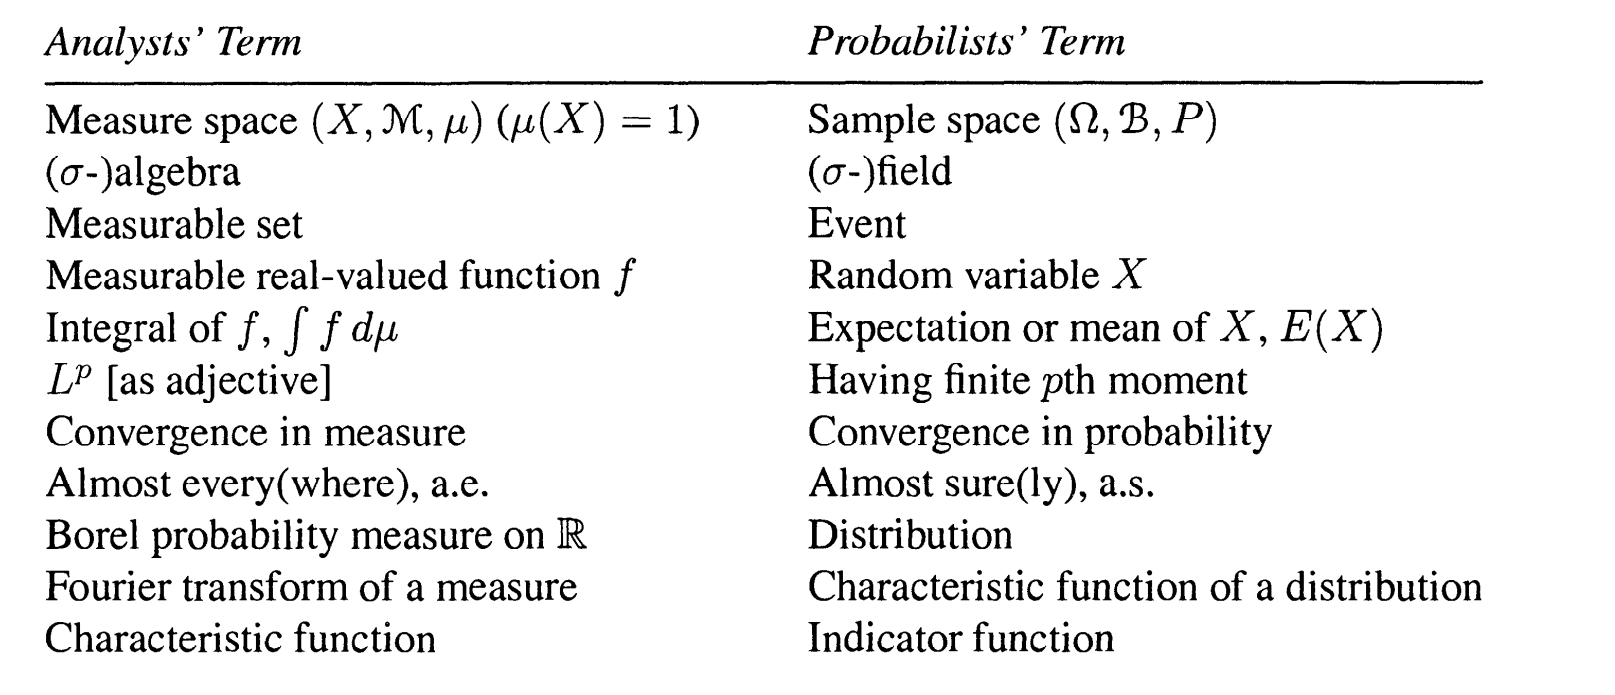
\includegraphics[scale=0.96]{Folland_screenshot.png}\retTwo\par}

Also, given some proposition $Q$, probabilists typically write $\{Q(\omega)\}$ as opposed to $\{\omega \in \Omega : Q(\omega) = \text{true}\}$. And given a probability measure $P$ they write $P(Q(\omega))$ as opposed to $P(\{Q(\omega)\})$. As long as I'm studying probability theory, I'm going to use probability terminology and notation.\retTwo

\hTwo Let $X$ be a random variable. We define it's \udefine{variance} $\sigma^2$ and \udefine{standard deviation} $\sigma$ as:\\ [-20pt]

{\center $\sigma^2(X) \coloneqq \inf_{a \in \mathbb{R}}E[(x - a)^2]$ and $\sigma(X) \coloneqq \sqrt{\sigma^2(X)}$\retTwo\par}

If $X \notin L^2$, then we always have $E((X - a)^2) = \infty$ for all $a$ and thus $\sigma^2(X) = \infty$. Otherwise, since $L^2 \subseteq L^1$ (since $P$ is finite), we have that $X \in L^1 \cap L^2$. So:

{\centering$E((X - a)^2) = E(X^2 - 2aX + a^2) = E(X^2) - 2aE(X) + a^2$.\newpage\par} 

Note that this is a quadratic which attains it's minimum at $a = E(X)$.
\begin{myIndent}\pracTwo
	Sanity check, by completing the square we have:
	
	{\center\fontsize{11}{13}\selectfont$a^2 - 2aE(X) = a^2 - 2aE(X) + (E(X))^2 - (E(X))^2 = (a - E(X))^2 - (E(X))^2$.\retTwo\par}
\end{myIndent}

Hence, for all $X \in L^2$ we have that:

{\centering$\sigma^2(X) = E(X^2) - 2(E(X))^2 + (E(X))^2 = E(X^2) - (E(X))^2$.\retTwo\par}

Let $(\Omega, \mathcalli{B}, P)$ be a sample space and let $(\Omega^\prime, \mathcalli{B}^\prime)$ be another measurable space. Given a $(\mathcalli{B}, \mathcalli{B}^\prime)$-measurable map $\phi$, we may define the \udefine{image measure} $P_\phi(E) \coloneqq P(\phi^{-1}(E))$ on $(\Omega^\prime, \mathcalli{B}^\prime)$. This is in fact a measure because preimages commute with unions, intersections, and complements. Also importantly $P_\phi(\Omega^\prime) = P(\Omega) = 1$. So $P_\phi$ is another probability measure.\retTwo

\exTwo\hypertarget{Folland Proposition 10.1}{\ul{Proposition 10.1:}} If $f: \Omega^\prime \to \mathbb{R}$ is a random variable, then $\int f \df P_\phi = \int (f \circ \phi) \df P$\\ whenever either side exists.

\begin{myIndent}\exThreeP
	This obviously holds for simple functions and you can extend the result from there using standard methods.\retTwo
\end{myIndent}

\hTwo If $X$ is a random variable on $\Omega$, then  $P_X$ is a probability measure on $\mathbb{R}$ called the\\ \udefine{distribution} of $X$. Also, we call $F(t) = P_X((-\infty, t]) = P(X \leq t)$ the \udefine{distribution\\ function} of $X$. If $\{X_\alpha\}_{\alpha \in A}$ is a family of random variables, we say that $\{X_\alpha\}_{\alpha \in A}$ are\\ \udefine{identically distributed} if $P_{X_\alpha} = P_{X_\beta}$ for all $\alpha, \beta \in A$.\retTwo

Basically all properties of a random variable we care about can be gathered just from\\ knowing the variable's distribution. For example, by proposition 10.1 we know that:

{\centering $E(X) = \int t \df P_X(t)$ and $E[(X - a)^2] = \int (t - a)^2 \df P_X(t)$. \retTwo\par}

\begin{myTindent}\pracTwo
	And from there we can easily see if $t \in L^1(P_X) \cap L^2(P_X)$, then:
	
	{\centering$\sigma^2(X) = \int (t - E(X))^2 \df P_X(t)$.\retTwo\par}
\end{myTindent}

If $X_1, \ldots, X_n$ is a finite sequence of random variables on $\Omega$, then we can consider\\ $(X_1, \ldots, X_n)$ as a map from $\omega$ to $\mathbb{R}^n$. Then the induced measure $P_{(X_1, \ldots, X_n)}$ on $\mathbb{R}^n$ is\\ called the \udefine{joint distribution} of $X_1, \ldots, X_n$.

\begin{myTindent}\pracOne
	Hopefully it's a given but if you doubt $(X_1, \ldots, X_n)$ is measurable\\ then see the proposition on page 41 of my math 240a latex notes.\retTwo
\end{myTindent}

Note by proposition 10.1 that given any two random variables $X, Y$ on $\Omega$:

{\center\begin{tabular}{l}
	$\int (t + s) \df P_{X, Y}(t, s) = \int [\pi_1 \circ \myId] \df P_{X, Y} + \int [\pi_2 \circ \myId] \df P_{X, Y}$\\ [6pt]
	$\phantom{\int (t + s) \df P_{X, Y}(t, s)} = \int [\pi_1 \circ \myId \circ (X, Y)] \df P + \int [\pi_2 \circ \myId \circ (X, Y)]\df P$\\ [6pt]
	$\phantom{\int (t + s) \df P_{X, Y}(t, s)} = \int X \df P + \int Y \df P = E(X) + E(Y) = E(X + Y)$.
\end{tabular}\retTwo\par}

Because of the convenience of distributions, given a Borel probability measure $\lambda$ on $\mathbb{R}$\\ we'll often talk of the mean $\overline{\lambda}$ and variance $\sigma^2(\lambda)$ of $\lambda$:

{\centering $\overline{\lambda} \coloneqq \int t \df \lambda(t)$ and $\sigma^2(\lambda) \coloneqq \int (t - \overline{\lambda})^2 \df \lambda(t)$ \newpage\par}

Let $(\Omega, \mathcalli{F}, P)$ be a sample space and $E \subseteq \Omega$ be an event such that $P(E) > 0$. Then\\ $P_E(F) \coloneqq P(E \cap F) / P(E)$ is a probability measure on $E$ which gives the \udefine{conditional\\ probability} of $F$ given $E$. $P_E(F)$ is also denoted $P(F | E)$.\retTwo

It's clear if $P(E) > 0$ that we then have that $P(E \cap F) = P(E)P(F | E)$. An important case to consider is when $P(F | E) = P(F)$ (which corresponds to when knowing $\omega \in E$ doesn't give us any information about if $\omega \in F$). In that case we say that $E$ and $F$ are\\ independent. More generally, we call two events $E$ and $F$ independent whenever\\ $P(E \cap F) = P(E)P(F)$. Even more generally, we call an arbitrary collection $\{E_\alpha\}_{\alpha \in A}$\\ of events in $\Omega$ \udefine{independent} iff for all $n \in \mathbb{N}$ and $\alpha_1, \ldots, \alpha_n \in A$, we have that\\ $P(\bigcap_{j=1}^n E_{\alpha_j}) = \prod_{j=1}^n P(E_{\alpha_j})$.\retTwo

\begin{myIndent}\pracOne
	From this definition hopefully it is obvious to you that if $C \subseteq A$, then $\{E_\alpha\}_{\alpha \in C}$\\ is a collection of independent random variables.\retTwo
\end{myIndent}

An arbitrary collection of random variables $\{X_\alpha\}_{\alpha \in A}$ are called \udefine{independent} if\\ $\{X_\alpha^{-1}(B_\alpha)\}_{\alpha \in A}$ is independent for all choices of $B_\alpha \in \mathcalli{B}_{\mathbb{R}}$.\retTwo

Observe that:

{\centering\begin{tabular}{l}
	$P(X_1^{-1}(B_1) \cap \ldots \cap X_n^{-1}(B_n)) = P((X_1, \ldots, X_n)^{-1}(B_1 \times \ldots \times B_n))$\\
	$\phantom{P(X_1^{-1}(B_1) \cap \ldots \cap X_n^{-1}(B_n))} = P_{X_1, \ldots, X_n}(B_1 \times \ldots \times X_n)$
\end{tabular}\retTwo\par}

Meanwhile $\prod_{j=1}^n P(X_j^{-1}(B_j)) = \prod_{j = 1}^n P_{X_j}(B_j) = \left(\prod_{j=1}^n P_{X_j}\right)(B_1 \times \ldots \times B_n)$.\retTwo

Thus, we have that $P_{X_1, \ldots, X_n} = \prod_{j=1}^n P_{X_j}$ if $X_1, \ldots, X_n$ are independent. Also, we\\ can easily show the converse by just setting $B_j = \mathbb{R}$ for any $j$ we want to ignore when\\ proving independence.\retTwo

\exTwo\hypertarget{Folland Proposition 10.2}{\ul{Proposition 10.2:}} Let $\{X_{n,j} : 1 \leq j \leq J(n), 1 \leq n \leq N\}$ be independent random variables, and let $f_n : \mathbb{R}^{J(n)} \to \mathbb{R}$ be Borel measurable for $1 \leq n \leq N$. Then the random variables $\{Y_n = f_n(X_{n,1}, \ldots, X_{n, J(n)}) : 1 \leq n \leq N\}$ are independent.

\begin{myIndent}\exThreeP
	Proof:\\
	Let $Z_n = (X_{n,1}, \ldots, X_{n, J(n)})$. If $B_1, \ldots, B_N$ are Borel subsets of $\mathbb{R}$, we have that\\ $Y_n^{-1}(B_n) = Z_n^{-1}(f_n^{-1}(B_n))$. Hence:\\ [-10pt]

	{\centering\begin{tabular}{l}
		$(Y_1, \ldots, Y_N)^{-1}(B_1 \times \ldots \times B_n) = \bigcap_{n=1}^N Y_n^{-1}(B_n)$\\ [4pt]
		$\phantom{(Y_1, \ldots, Y_N)^{-1}(B_1 \times \ldots \times B_n)} = \bigcap_{n=1}^N Z_n^{-1}(f_n^{-1}(B_n))$ \\ [4pt]
		$\phantom{(Y_1, \ldots, Y_N)^{-1}(B_1 \times \ldots \times B_n)} = (Z_1, \ldots, Z_N)^{-1}(f_1^{-1}(B_1) \times \ldots \times f_N^{-1}(B_N))$
	\end{tabular}\retTwo\par}

	But now note that $(Z_1, \ldots, Z_n)$ and $(X_{1,1},\ldots,X_{N,J(N)})$ are identical functions. And so by the independence of the $X_{n,j}$ and \inLinkRap{Folland Exercise 2.45}{Exercise 2.45}, note that:

	{\center\begin{tabular}{l}
		$P_{Z_1, \ldots, Z_n} = P_{X_{1,1},\ldots,X_{N,J(N)}}$\\
		
		$\phantom{P_{Z_1, \ldots, Z_n}} = \hspace{-0.6em}\prod\limits_{n=1,\phantom{.} j=1}^{N,\phantom{.} J(n)}\hspace{-0.6em} P_{X_{n,j}} = \prod\limits_{n=1}^N \left( \prod\limits_{j=1}^{J(n)} P_{X_{n,j}}\right) = \prod\limits_{n=1}^N \left(P_{X_{n,1}, \ldots, X_{n, J(n)}}\right) = \prod_{n=1}^N P_{Z_n}$
	\end{tabular}\newpage\par}

	Therefore, we have that:

	{\centering\begin{tabular}{l}
		$P_{Y_1, \ldots, Y_N}(B_1 \times \ldots \times B_N) = P((Y_1, \ldots, Y_N)^{-1}(B_1 \times \ldots \times B_N))$\\ [4pt]

		$\phantom{P_{Y_1, \ldots, Y_N}(B_1 \times \ldots \times B_N)} = P((Z_1, \ldots, Z_N)^{-1}(f_1^{-1}(B_1) \times \ldots \times f_N^{-1}(B_N)))$\\ [4pt]

		$\phantom{P_{Y_1, \ldots, Y_N}(B_1 \times \ldots \times B_N)} = P_{Z_1, \ldots, Z_n}(f_1^{-1}(B_1) \times \ldots \times f_N^{-1}(B_N))$\\ [4pt]

		$\phantom{P_{Y_1, \ldots, Y_N}(B_1 \times \ldots \times B_N)} = \prod_{n=1}^N P_{Z_n}(f_n^{-1}(B_n))$\\ [4pt]

		$\phantom{P_{Y_1, \ldots, Y_N}(B_1 \times \ldots \times B_N)} = \prod_{n=1}^N P(Z_n^{-1}(f_n^{-1}(B_n)))$\\ [4pt]

		$\phantom{P_{Y_1, \ldots, Y_N}(B_1 \times \ldots \times B_N)} =  \prod_{n=1}^N P(Y_n^{-1}(B_n)) = \prod_{n=1}^N P_{Y_n}(B_n)$. $\blacksquare$
	\end{tabular}\retTwo\par}
\end{myIndent}

\dispDate{9/15/2025}

\pracOne\ul{Quick lemma:} Let $(\Omega_1, \mathcalli{F}_1, P)$ be a sample space, let $(\Omega_2, \mathcalli{F}_2)$, $(\Omega_3, \mathcalli{F}_3)$ be measurable\\ spaces, and let $\phi: \Omega_1 \to \Omega_2$, $\psi: \Omega_2 \to \Omega_3$ be measurable maps. Then $P_{\psi \circ \phi} = (P_\phi)_{\psi}$.

\begin{myIndent}\pracTwo
	Proof:

	{\centering $P_{\psi \circ \phi}(E) = P((\psi \circ \phi)^{-1}(E)) = P(\phi^{-1}(\psi^{-1}(E))) = P_\phi(\psi^{-1}(E)) = (P_\phi)_{\psi}(E)$.\retTwo\par}

	\myComment (I'm mentioning this because Folland implicitely uses this in the next proof\dots)\retTwo
\end{myIndent}

\hTwo By easy induction on our proof for \inLinkRap{Folland Proposition 8.48 part a}{proposition 8.48(a)}, we can see that if $\lambda_1, \ldots, \lambda_n$ are\\ all in $M(\mathbb{R}^n)$, then:

{\centering$\lambda_1 * \ldots * \lambda_n(E) = \int\cdots\int \chi_E(\sum_{i=1}^n t_n) \df \lambda_1(t_1)\cdots \df \lambda_n(t_n)$.\retTwo\par}

\exTwo\hypertarget{Folland Proposition 10.4}{\ul{Proposition 10.4:}} If $X_1, \ldots, X_n$  are independent random variables, then:

{\centering $P_{X_1 + \ldots + X_n} = P_{X_1} * \ldots * P_{X_n}$.\par}

\begin{myIndent}\exThreeP
	Proof:\\
	Let $A(t_1, \ldots, t_n) = \sum_{j=1}^n t_j$. Then $A$ is a Borel measurable map from $\mathbb{R}^n$ to $\mathbb{R}$. So:

	{\center\begin{tabular}{l}
		$P_{X_1 + \ldots + X_n}(E) = \left(P_{X_1, \ldots, X_n}\right)_A(E)$\\ [8pt]
		$\phantom{P_{X_1 + \ldots + X_n}(E)} = \left(\prod_{j=1}^n P_{X_j}\right)_A(E) = \left(\prod_{j=1}^n P_{X_j}\right)(A^{-1}(E))$\\ [8pt]
		$\phantom{P_{X_1 + \ldots + X_n}(E) = \left(\prod_{j=1}^n P_{X_j}\right)_A(E)} = (P_{X_1} * \ldots * P_{X_n})(E)$. $\blacksquare$
	\end{tabular}\retTwo\par}
\end{myIndent}

\ul{Propostion 10.5:} Suppose that $X_1, \ldots, X_n$ are independent random variables. If $X_j \in L^1$ for all $1 \leq j \leq n$, then $\prod_{j=1}^n X_j \in L^1$ and $E(\prod_{j=1}^n X_j) = \prod_{j=1}^n E(X_j)$.

\begin{myIndent}\exThreeP
	Proof:\\
	Let $f(t_1, \ldots, t_n) = \prod_{j=1}^n |t_j|$. Then by the independence of the $X_j$ we have that:\\ [-8pt]

	{\centering\begin{tabular}{l}
		$E(\left|\prod_{j=1}^n X_j\right|) = \int f \circ (X_1, \ldots, X_n) \df P = \int f \df P_{X_1, \ldots, X_n} = \int f \df(P_{X_1} \times \ldots \times P_{X_n})$
	\end{tabular}\retTwo\par}

	And since $f$ is nonnegative, we know by Tonelli's theorem that:\\ [-10pt]

	{\center\begin{tabular}{l}
		$\int f \df(P_{X_1} \times \ldots \times P_{X_n}) = \prod_{j=1}^n \int |t_j| \df P_{X_j} = \prod_{j=1}^n E(|X_j|)$
	\end{tabular}\retTwo\par}

	Hence if all the $X_j \in L^1$, we've shown that $E(\left|\prod_{j=1}^n X_j\right|) = \prod_{j=1}^n E(|X_j|) < \infty$. This proves our first assertion that $\prod_{j=1}^n X_j \in L^1$. And to our prove our second assertion, just do the prior reasoning all over again but remove all the absolute value signs and use Fubini's theorem instead of Tonelli's. $\blacksquare$\newpage
\end{myIndent}

\hypertarget{Folland Corollary 10.6}{\ul{Corollary 10.6:}} Suppose that $X_1, \ldots, X_n$ are independent random variables and in $L^2$. Then $\sigma^2(X_1 + \ldots + X_n) = \sum_{j=1}^n \sigma^2(X_j)$.\retTwo

\begin{myIndent}\exThreeP
	Proof:\\
	Let $Y_j = X_j - E(X_j)$. Then by proposition 10.2, we have that all the $Y_j$ are independent and have an expected value of $0$. So by our last proposition, we know for all $j \neq k$ that $E(Y_j Y_k) = E(Y_j)E(Y_k) = 0$. And hence:

	{\centering\begin{tabular}{l}
		$\sigma^2(X_1 + \ldots + X_n) = E((X_1 + \ldots + X_n - E(X_1 + \ldots + X_n))^2)$\\ [4pt]
		$\phantom{\sigma^2(X_1 + \ldots + X_n)} = E((Y_1 + \ldots + Y_n)^2)$\\ [2pt]
		$\phantom{\sigma^2(X_1 + \ldots + X_n)} = \sum\limits_{j=1}^n\sum\limits_{k=1}^n E(Y_j Y_k) = \sum\limits_{j=1}^n E(Y_j^2) = \sum\limits_{j=1}^n \sigma^2(X_j)$. $\blacksquare$
	\end{tabular}\retTwo\par}
\end{myIndent}

\hTwo These prior properties show us that independence is actually a very strong assumption to make. In fact, by propositions 10.2 and 10.5, if $X$ and $Y$ are independent random variables with $E(X) = 0$, then given any Borel measurable function $f$ such that $f \circ Y \in L^1$, we have that $E(X \cdot f(Y)) = E(X)E(f(Y)) = 0$. Hence $X$ is orthogonal in $L^2$ to every function of $Y$ with finite $2$nd moment.\retTwo

That said, fortunately there is an easy way of constructing collections of independent\\ random variables. Specifically, given a collection of sample spaces $\{(\Omega_j, \mathcalli{B}_j, P_j)\}_{j=1}^n$, let\\ $\Omega = \Omega_1 \times \ldots \times \Omega_n$, $\mathcalli{B} = \mathcalli{B}_1 \otimes \ldots \otimes \mathcalli{B}_n$, and $P = P_1 \times \ldots \times P_n$. Then any collection\\ $\{X_1, \ldots, X_n\}$ of random variables on $\Omega$ such that $X_j$ depends only on the $j$th. coordinate\\ of $\Omega$ for each $j$ is independent.

\begin{myIndent}\pracTwo
	After all, express every $X_j$ as $f_j \circ \pi_j$ where $f_j$ is some $\mathcalli{B}_j$-measurable function and $\pi_j$\\ is the projection of $\Omega$ onto $\Omega_j$. Now given any rectangle $B_1 \times \ldots \times B_n$ in $\mathcalli{B}_{\mathbb{R}^n}$, we have\\ that:

	{\centering\begin{tabular}{l}
		$P_{X_1, \ldots, X_n}(B_1 \times \ldots \times B_n) = P((X_1, \ldots, X_n)^{-1}(B_1 \times \ldots \times B_n))$\\ [1pt]
		$\phantom{P_{X_1, \ldots, X_n}(B_1 \times \ldots \times B_n)} = P(\prod\limits_{j=1}^n f_j^{-1}(B_j)) = \prod\limits_{j=1}^n P_j(f_j^{-1}(B_j)) = \prod\limits_{j=1}^N (P_j)_{f_j}(B_j)$.
	\end{tabular}\retTwo\par}

	Now it is easily seen that:
	
	{\centering\begin{tabular}{l}
		$P_{\pi_j}(E) = P(\Omega_1 \times \ldots \times \Omega_{j-1} \times E \times \Omega_{j+1} \times \ldots \times \Omega)$\\ [1pt]
		$\phantom{P_{\pi_j}(E)} = P_j(E) \cdot \prod\limits_{i\neq j}P_i(\Omega_i) = P_j(E) \cdot 1 = P_j(E)$
	\end{tabular}\retTwo\par}

	Thus $(P_j)_{f_j} = (P_{\pi_j})_{f_j} = P_{f_j \circ \pi_j} = P_{X_j}$ and we've shown that $P_{X_1, \ldots, X_n}$ and\\ [1pt] $\prod_{j=1}^n P_{X_j}$ agree on all rectangles. It now follows by standard arguments that they\\ equal for all sets in $\mathcalli{B}_{\mathbb{R}^n}$.
\end{myIndent}

\Hstatement\mySepTwo

\blab{Exercise 10.9:} Suppose that $(X_n)_{n \in \mathbb{N}}$ is a sequence of random variables. If $X_n \to X$ in\\ probability, then $P_{X_n} \to P_X$ vaguely. 

\begin{myIndent}\HexOne
	Note that we trivially have that $\sup_{n \in \mathbb{N}} \|P_{X_n}\| = 1 < \infty$ since all the $P_{X_n}$ are probability\\ [1pt] measures. Meanwhile, define $F_n(t) \coloneqq P_{X_n}((-\infty, t])$ and $F(t) \coloneqq P_{X_n}((-\infty, t])$. We\\ [1pt] want to show that if $F$ is continuous at $t_0 \in \mathbb{R}$ then we have that $F_n(t_0) \to F(t_0)$ as\\ [1pt] $n \to \infty$. This is so that we can then apply \inLinkRap{Folland Proposition 7.19}{proposition 7.19} and be done.\newpage 
	
	So given any $\varepsilon > 0$, use the continuity of $F$ at $t_0$ to pick $\delta > 0$ such that $|F(t) - F(t_0)| < \varepsilon$ whenever $|t - t_0| < \delta$. Since $X_n \to X$ in measure, we may pick $N > 0$ such that $P(|X_n - X| > \sfrac{\delta}{2}) < \varepsilon$ for all $n \geq N$. Also, let $E_n = \{|X_n - X| \leq \sfrac{\delta}{2}\}$ for all $n \geq N$. Thus we have for all $n \geq N$ that:\\ [-6pt]

	{\centering\begin{tabular}{l}
		$|F_n(t_0) - F(t_0)| = |P(X_n^{-1}((-\infty, t_0]) \cap E_n) + P(X_n^{-1}((-\infty, t_0]) \cap E_n^\comp)$\\ [2pt]
		$\phantom{|F_n(t_0) - F(t_0)| = aaaaaaa} - P(X^{-1}((-\infty, t_0 + \sfrac{\delta}{2}])) + P(X^{-1}(( t_0, t_0 + \sfrac{\delta}{2}])) |$\\ [8pt]

		$\phantom{|F_n(t_0) - F(t_0)|} \leq |P(X_n^{-1}((-\infty, t_0]) \cap E_n) - P(X^{-1}((-\infty, t_0 + \sfrac{\delta}{2}]))|$\\ [2pt]
		$\phantom{|F_n(t_0) - F(t_0)| = aaaaaaa} + |P(X_n^{-1}((-\infty, t_0]) \cap E_n^\comp) + P(X^{-1}((t_0, t_0 + \sfrac{\delta}{2}]))|$
	\end{tabular} \retTwo\par}

	Now because $P(E_n^\comp) < \varepsilon$ and $|P(X^{-1}((t_0, t_0 + \sfrac{\delta}{2}]))| = |F(t_0 + \sfrac{\delta}{2}) - F(t_0)| < \varepsilon$, we know that $|P(X_n^{-1}((-\infty, t_0]) \cap E_n^\comp) + P(X^{-1}((t_0, t_0 + \sfrac{\delta}{2}]))| < 2\varepsilon$.\retTwo

	Meanwhile, $X_n^{-1}((-\infty, t_0]) \cap E_n \subseteq X^{-1}((-\infty, t_0 + \sfrac{\delta}{2}])$. Therefore, we have that:\\ [-6pt]

	{\centering\begin{tabular}{l}
		$|P(X_n^{-1}((-\infty, t_0]) \cap E_n) - P(X^{-1}((-\infty, t_0 + \sfrac{\delta}{2}]))|$\\ [4pt]
		$\phantom{aaaaaaaaaaaa} = P(X^{-1}((-\infty, t_0 + \sfrac{\delta}{2}]) - (E_n \cap X_n^{-1}((-\infty, t_0])))$\\ [4pt]
		$\phantom{aaaaaaaaaaaa} < P(E_n^\comp) + P(E_n \cap \left(X^{-1}((-\infty, t_0 + \sfrac{\delta}{2}] - X_n^{-1}((-\infty, t_0]))\right)) < \varepsilon + 0$
	\end{tabular} \retTwo\par}

	So $|F_n(t_0) - F(t_0)| < 3\varepsilon$ for all $n \geq N$. This proves that $F_n(t_0) \to F(t_0)$ as $n \to \infty$ and we are done. $\blacksquare$\retTwo
\end{myIndent}

\blab{Exercise 10.4:} Let $X$, $Y$, and $Z$ be positive independent random variables with a common\\ distribution $\lambda$, and let $F(t) = \lambda((-\infty, t])$. The probability that the polynomial $X t^2 + Y t + Z$\\ has real roots is $\int_0^\infty \int_0^\infty F(t^2 / 4s) \df \lambda(t) \df \lambda(s)$.

\begin{myIndent}\HexOne
	This is really easy. Note that the quadratic has real roots iff $Y^2 - 4XZ \geq 0$. Rewriting this, we have that the quadratic has real roots when $0 \leq Z \leq Y^2 / 4X$. Therefore:
	
	{\centering\begin{tabular}{l}
		$P(Y^2 - 4XZ \geq 0) = \int \chi_{\{t^2 - 4rs \geq 0\}}\df P_{X, Y, Z}(r, s, t)$\\ [4pt]
		
		$\phantom{P(Y^2 - 4XZ \geq 0)} = \int \chi_{\{t^2 - 4rs \geq 0\}}\df \lambda^3(r, s, t)$\\ [2pt]
		
		$\phantom{P(Y^2 - 4XZ \geq 0)} = \int_0^\infty \int_0^\infty \int_0^{t^2/4s} \df \lambda(r)\df \lambda(t)\df \lambda(s)$\\ [4pt]

		$\phantom{P(Y^2 - 4XZ \geq 0)} = \int_0^\infty \int_0^\infty F(t^2 / 4s) \df \lambda(t) \df \lambda(s)$. $\blacksquare$
	\end{tabular}\retTwo\par}
\end{myIndent}

\blab{Exercise 10.5:} If $X$ is a random variable with distribution $P_X = f(t)\df t$ where $f(t) = f(-t)$,\\ then the distribution of $X^2$ is $P_{X^2} = t^{-1/2} f(t^{1/2})\chi_{(0, \infty)}(t) \df t$.

\begin{myIndent}\HexOne
	Note that for any $s \geq 0$, $\{X^2 \leq s\} = \{-\sqrt{s} \leq X \leq \sqrt{s}\}$. Hence:

	{\centering\begin{tabular}{l}
		$P_{X^2}((-\infty, s]) = P(X^2 \leq s) = P(-\sqrt{s} \leq X \leq \sqrt{s})$\\ [4pt]
		$\phantom{P_{X^2}((-\infty, s]) = P(X^2 \leq s)} = \int_{-\sqrt{s}}^{\sqrt{s}} \df P_X = \int_{-\sqrt{s}}^{\sqrt{s}} f(t)\df t = \int_0^{\sqrt{s}}2f(t)\df t$\\ [4pt]
		$\phantom{P_{X^2}((-\infty, s]) = P(X^2 \leq s) = \int_{-\sqrt{s}}^{\sqrt{s}} \df P_X = \int_{-\sqrt{s}}^{\sqrt{s}} f(t)\df t} = \int_0^{s}2f(u^{1/2})(\frac{1}{2}u^{-1/2}\df u)$\\ [4pt]
		$\phantom{P_{X^2}((-\infty, s]) = P(X^2 \leq s) = \int_{-\sqrt{s}}^{\sqrt{s}} \df P_X = \int_{-\sqrt{s}}^{\sqrt{s}} f(t)\df t} = \int_0^s u^{-1/2}f(u^{1/2})\df u$
	\end{tabular}\retTwo\par}

	Meanwhile if $s < 0$, then $P_{X^2}((-\infty, s]) = 0$. Hence, we have for all $s \in \mathbb{R}$ that:

	{\centering $P_{X^2}((-\infty, s]) = \int_{-\infty}^s t^{-1/2}f(t^{1/2})\chi_{(0, \infty)}\df t$ \retTwo\par}

	This is enough by theorem 3.29 (see my math 240a paper notes) that to see that\\ $P_{X^2} = t^{-1/2}f(t^{1/2})\chi_{(0, \infty)}\df t$. $\blacksquare$\newpage
\end{myIndent}

I won't be reintroducing distributions or proving things that are already in my math 180a notes. That said, there is a result I'd like to give more clarity to. To start off, Folland denotes:

\begin{itemize}
	\item $\delta_t$ (where $t \in \mathbb{R}$) is the point mass measure centered at $E$ (meaning $\delta_t(E) = 1$ if $t \in E$\\ and $0$ otherwise).
	
	\item $\beta_p^{*n} \coloneqq \sum_{k=0}^n \binom{n}{k}p^k(1 - p)^{n-k}\delta_k$ is the binomial distribution with parameters $n \in \mathbb{N}$ and $p \in [0, 1]$.
	
	\item $\lambda_a \coloneqq e^{-a}\sum_{k=0}^\infty \frac{a^k}{k!}\delta_k$ is the Poisson distribution with parameter $a > 0$.
\end{itemize}

\blab{Exercise 10.8(c):} $\beta_{a/n}^{*n} \to \lambda_a$ vaguely as $n \to \infty$.

\begin{myIndent}\HexOne
	Like in my answer to exercise 10.9, our strategy for this exercise will be to apply \inLinkRap{Folland Proposition 7.19}{proposition\\ [2pt] 7.19}. So, set $F_n(t) \coloneqq \beta_{a/n}^{*n}((-\infty, t])$ and $F(t) \coloneqq \lambda_a((-\infty, t])$ for all $t \in \mathbb{R}$. Then the\\ set of discontinuities of $F$ is precisely $\mathbb{N}$ (here I'm having $\mathbb{N}$ include $0$). So, we just need to\\ [2pt] show that $F_n(t) \to F(t)$ whenever $t \notin \mathbb{N}$.\retTwo
	
	If $t < 0$, then it's clear that $0 = F_n(t) \to F(t) = 0$ as $n \to \infty$. Meanwhile, suppose that\\ [-1pt] $N < t < N + 1$ where $N \in \mathbb{N}$. Then $F(t) = e^{-a}\sum_{k=0}^N \frac{a^k}{k!}$.\retTwo 
	
	Meanwhile $\frac{n(n-1)\cdots(n-k+1)}{n^k} \to 0$, $(1 - \frac{a}{n})^n \to e^{-a}$, and $(1 - \frac{a}{n})^{-k} \to 1^{-k} = 1$ as $n \to \infty$\\ for all $k$. Therefore for $N < t < N+1$ we have:
	
	{\centering$F_n(t) = \sum_{k=0}^N \binom{n}{k} (\sfrac{a}{n})^k (1 - \sfrac{a}{n})^{n-k} \to \sum_{k=0}^N \frac{a^ke^{-a}}{k!} = F(t)$ as $n \to \infty$. $\blacksquare$\retTwo\par}

	\myComment\fontsize{11}{13}\selectfont As a side note, since $\|\beta_{a/n}^{*n}\| = 1 = \|\lambda_a\|$ for all $n$ since all of them are probability measures, we can apply \inLinkRap{Folland exercise 7.26}{Exercise 7.26} to say that $\int f \df \beta_{a/n}^{*n} \to \int f \df \lambda_a$ as $n \to \infty$ for all $f \in BC(\mathbb{R})$.\retTwo
\end{myIndent}

\blab{Exercise 10.10: (The Moment Convergence Theorem)}
\begin{myIndent}
	Let $X_1, X_2, \ldots, X$ be random variables such that $P_{X_n} \to P_X$ vaguely and\\ $\sup_{n \in \mathbb{N}}E(|X_n|^r) < \infty$ for some $r > 0$. Then $E(|X_n|^s) \to E(|X|^s)$ for all\\ $s \in (0, r)$, and if $s \in \mathbb{N}$ also, then $E((X_n)^s) \to E(X^s)$.\retTwo

	\HexOne Proof:\\
	Fix $C \geq \sup_{n \in \mathbb{N}} E(|X_n|^r)$. Then by Chebyshev's inequality (see my math 240b notes),\\ we know that $P(|X_n| > \alpha) \leq \frac{E(|X_n|^r)}{\alpha^r}$ for all $\alpha > 0$ and $n \in \mathbb{N}$. And hence for all $n \in \mathbb{N}$ we have that $P(|X_n| > \alpha) \leq C/\alpha^r$ when $\alpha > 0$.\retTwo

	Next, given any $\alpha > 0$, let $\phi_\alpha \in C_c(\mathbb{R}, [0, 1])$ such that $\phi_{\alpha}(t) = 1$ when $|t| \leq \alpha$ and\\ $\phi_{\alpha}(t) = 0$ when $|t| > \alpha + 1$. Importantly, $\phi_\alpha(t)|t|^s$ (and $\phi_\alpha(t) t^s$ when $s$ is an\\ integer) is in $C_c(\mathbb{R})$. Thus by the vague convergence of the $P_{X_n}$ we know for all $s \in (0, r)$\\ that $\int \phi_{\alpha}(t)|t|^s\df P_{X_n} \to \int \phi_{\alpha}(t)|t|^s \df P_{X}$ as $n \to \infty$ (and similarly if $s$ is also an integer\\ we have that $\int \phi_{\alpha}(t)t^s\df P_{X_n} \to \int \phi_{\alpha}(t)t^s \df P_{X}$).\retTwo

	Meanwhile, since $s < r$, we know by Hölder's inequality that:

	{\centering\begin{tabular}{l}
		$0 \leq \int (1 - \phi_{\alpha}(t))|t|^s \df P_{X_n} \leq \left[\int (1 - \phi_{\alpha}(t))^{r/(r-s)} \df P_{X_n}\right]^{(r-s)/r} \cdot \left[\int \left(|t|^s\right)^{r/s} \df P_{X_n}\right]^{s/r}$\\ [4pt]
		$\phantom{0 \leq \int (1 - \phi_{\alpha}(t))|t|^s \df P_{X_n}} \leq [\int \chi_{\{|t| > a\}} \df P_{X_n}]^{(r-s)/r} \cdot [E(|X_n|^r)]^{s/r}$\\ [4pt]
		$\phantom{0 \leq \int (1 - \phi_{\alpha}(t))|t|^s \df P_{X_n}} \leq (P(|X_n| > a))^{(r-s)/r} \cdot C^{s/r} \leq (\frac{C^{1/r}}{\alpha})^{r-s}C^{s/r} = \frac{C}{\alpha^{r-s}}$.
	\end{tabular}\newpage\par}

	Now $\int |t|^s\df P_{X_n} = \int \phi_{\alpha}(t)|t|^s \df P_{X_n} + \int(1 - \phi_{\alpha}(t))|t|^s \df P_{X_n}$. So, we can say that:\\ [-6pt]

	{\centering\begin{tabular}{l}
		$\int_{-\alpha}^{\alpha} |t|^s \df P_{X} \leq \int \phi_{\alpha}(t)|t|^s \df P_{X} \leq \liminf\limits_{n \to \infty} \int |t|^s \df P_{X_n}$\\ [10pt] 
		
		$\phantom{\int_{-\alpha}^{\alpha} |t|^s \df P_{X} \leq \int \phi_{\alpha}(t)|t|^s \df P_{X}} \leq \limsup\limits_{n \to \infty} \int |t|^s \df P_{X_n} \leq \int \phi_{\alpha}(t)|t|^s \df P_{X} + \frac{C}{\alpha^{r-s}}$\\ [10pt]

		$\phantom{\int_{-\alpha}^{\alpha} |t|^s \df P_{X} \leq \int \phi_{\alpha}(t)|t|^s \df P_{X} \leq \limsup\limits_{n \to \infty} \int |t|^s \df P_{X_n}} \leq \int_{-\alpha-1}^{\alpha + 1} |t|^s \df P_{X} + \frac{C}{\alpha^{r-s}}$
	\end{tabular}\retTwo\par}

	And by taking $\alpha \to \infty$, we know by the monotone convergence theorem and the fact that $\frac{1}{\alpha^{r-s}} \to 0$ that $\lim_{n \to \infty}E(|X|^s) = \lim_{n\to\infty}\int |t|^s \df P_{X_n} = \int |t|^s \df P_X = E(|X|^s)$ for all $s \in (0, r)$.\retTwo

	A notable consequence of this is that $X \in L^s(P)$ for all $s \in (0, r)$. After all, by Folland proposition 6.12 (see my math 240b notes):
	
	{\centering $\|X_n\|_s \leq \|X_n\|_rP(X)^{\sfrac{1}{s} - \sfrac{1}{r}} = \|X_n\|_r \leq C^{1/r}$ for all $n \in \mathbb{N}$.\retTwo\par}

	Thus $(E(|X_n|^s))_{n \in \mathbb{N}}$ is a sequence bounded above by $C^{s/r}$, and since $E(|X_n|^s) \to E(|X|^s)$, we have that $E(|X|^s) \leq C^{s/r} < \infty$ for all $s \in (0, r)$. This now let's us address the special case that $s$ is an integer. After all, note that:

	{\centering\begin{tabular}{l}
		$\limsup_{n\to\infty}|\int t^s \df P_{X_n} - \int t^s \df P_X| = \limsup_{n\to\infty}|\int t^s\phi_\alpha(t) \df P_{X_n} + \int t^s(1-\phi_\alpha(t)) \df P_{X_n}$\\ [6pt]
		$\phantom{aaaaaaaaaaaaaaaaaaaaaaaaaaaaaaaaaa} - \int t^s \phi_{\alpha}(t) \df P_X - \int t^s (1- \phi_\alpha(t)) \df P_X|$\\ [10pt]

		$\phantom{\limsup_{n\to\infty}|\int t^s \df P_{X_n} - \int t^s \df P_X|} \leq 0 + \limsup_{n\to\infty}|\int t^s(1 - \phi_{\alpha}(t))\df P_{X_n}|$\\ [2pt]
		$\phantom{aaaaaaaaaaaaaaaaaaaaaaaaaaaaaaaaaa 0 +}  + \limsup_{n \to \infty}|\int t^s(1 - \phi_{\alpha}(t))\df P_{X}|$
	\end{tabular}\retTwo\par}

	Now $0 \leq |\int (1 - \phi_{\alpha}(t))t^s \df P_{X_n}| \leq \int (1 - \phi_{\alpha}(t))|t|^s \df P_{X_n} \leq \frac{C}{\alpha^{r-s}}$ for all $n$.\retTwo
	
	Meanwhile pick $q \in (s, r)$ and note by Chebyshev's inequality that $P(|X| > \alpha) \leq \frac{C^{q/r}}{\alpha^{q}}$\\ [2pt] for all $\alpha > 0$. And then by similar reasoning to earlier we can show using Hölder's inequality\\ [2pt] that:

	{\centering\begin{tabular}{l}
		$0 \leq |\int (1 - \phi_{\alpha}(t))t^s \df P_{X}| \leq \int (1 - \phi_{\alpha}{t})|t|^s \df P_X$\\ [6pt]
		$\phantom{0 \leq |\int (1 - \phi_{\alpha}(t))t^s \df P_{X}|} \leq (P(|X| > \alpha))^{(q-s)/q} \cdot [E(|X|^q)]^{s/q}$\\ [6pt]
		$\phantom{0 \leq |\int (1 - \phi_{\alpha}(t))t^s \df P_{X}|} \leq (\frac{C^{1/r}}{\alpha})^{q-s} \cdot [C^{q/r}]^{s/q} = \frac{1}{\alpha^{q-s}} C^{(\frac{q}{r} - \frac{s}{r} + \sfrac{s}{r})} = \frac{1}{\alpha^{q-s}} C^{q/r}$
	\end{tabular} \retTwo\par}

	Thus $\limsup_{n\to\infty}|\int t^s \df P_{X_n} - \int t^s \df P_X| \leq \frac{C}{\alpha^{r-s}} + \frac{1}{\alpha^{q-s}} C^{q/r}$ and the latter goes to zero as $\alpha \to \infty$. $\blacksquare$\retTwo
\end{myIndent}

\mySepTwo

\hTwo\dispDate{9/16/2025}

\hypertarget{page 199 reference}{In} the next section of Folland, he writes a lot of theorems involving infinite sequences of\\ independent random variables. Now unfortunately actually constructing those sequences\\ requires some theorems I skipped over earlier. So for now just I'm just going to ignore the\\ issue. However, I'll come back and address this issue later on \inLinkRap{page 215 reference}{page 215}.\newpage

\exTwo\ul{Theorem 10.9: (The Weak Law of Large Numbers)}
\begin{myIndent}
	Let $\{X_j\}_{j = 1}^\infty$ be a sequence of independent $L^2$ random variables with means $\{\mu_j\}_{j \in \mathbb{N}}$ and variances $\{\sigma_j^2\}$. If $n^{-2}\sum_{j=1}^n \sigma^2_j \to 0$ as $n \to \infty$, then $n^{-1}\sum_{j=1}^n (X_j - \mu_j) \to 0$ in probability as $n \to \infty$.\retTwo

	\exThreeP Proof:\\
	$n^{-1}\sum_{j=1}^n (X_j - \mu_j)$ has mean $n \cdot 0 = 0$ and variance:
	
	{\centering$\sum_{j=1}^n (\sigma^2(\frac{X_j - \mu_j}{n})) = \sum_{j=1}^n(E(\frac{(X_j - \mu_j)^2}{n^2} - 0)) = \frac{1}{n^2}\sum_{j=1}^n \sigma^2(X_j)$.\retTwo\par}

	Hence by Chebyshev's inequality, for any $\varepsilon > 0$ we have that:

	{\centering $P(|n^{-1}\sum_{j=1}^n (X_j - \mu_j)| > \varepsilon) \leq \frac{1}{\varepsilon^2}\left(\frac{1}{n^2}\sum_{j=1}^n \sigma^2(X_j)\right)$ \retTwo\par}

	And since $n^{-2}\sum_{j=1}^n \sigma^2_j \to 0$ as $n \to \infty$, we know $P(|n^{-1}\sum_{j=1}^n (X_j - \mu_j)| > \varepsilon) \to 0$\\ as $n \to \infty$. $\blacksquare$\retTwo

	\begin{myIndent}\myComment
		As a side note: if $\sup_{j \in \mathbb{N}}\sigma^2_j \leq C < \infty$, then $n^{-2}\sum_{j=1}^n \sigma^2_j \leq n^{-1} C \to 0$ as\\ $n \to \infty$. Hence, this theorem is especially useful for the case where all the $X_j$\\ are identically distributed.\retTwo
	\end{myIndent}
\end{myIndent}

\Hstatement\mySepTwo
Before continuing, we need an exercise.\retTwo

\blab{Exercise 10.3(b):} Suppose that $\{E_\alpha\}_{\alpha \in A}$ is a collection of independent events in $\Omega$. Then so is $\{F_\alpha\}_{\alpha \in A}$ where each $F_\alpha$ is equal to either $E_\alpha$ or $E_\alpha^\comp$.

\begin{myIndent}\HexOne
	Proof:\\
	I already showed in my math 180a notes that this is true whenever $A$ is finite. So I won't be repeating that proof. In the general case, for any $n \in \mathbb{N}$ and $\alpha_1, \ldots, \alpha_n \in A$ we know that the subcollection $\{E_{\alpha_1}, \ldots, E_{\alpha_n}\}$ is also a collection of independent events. And so we can apply the finite case proved in my math 180a notes to say that $F_{\alpha_1}, \ldots, F_{\alpha_n}$ are independent events, and in turn that $P(\bigcap_{j=1}^n F_{\alpha_j}) = \prod_{j=1}^n P(F_{\alpha_j})$. $\blacksquare$
\end{myIndent}
\mySepTwo

\hTwo Given a sequence $\{A_n\}_{n \in \mathbb{N}}$ of measurable sets / events, we define:

{\centering$\limsup A_n \coloneqq \bigcap_{n \in \mathbb{N}}\left(\bigcup_{k=n}^\infty A_k\right)$ and $\liminf A_n \coloneqq \bigcup_{n \in \mathbb{N}}\left(\bigcap_{k=n}^\infty A_k\right)$\retTwo\par}

\begin{myIndent}\myComment
	For some intuition: 
	\begin{itemize}
		\item $x \in \liminf A_n \Longleftrightarrow \exists N > 0 \suchthat \forall n \geq N, \myHS x \in A_n$\\$\phantom{aaaaaaaaaaaaaaaaaaaaaaaaaaaaaaa}$ (i.e. $x$ is eventually in each $A_n$),
		
		\item $x \in \limsup A_n \Longleftrightarrow \forall N > 0,\myHS \exists n \geq N \suchthat x \in A_n$\\$\phantom{aaaaaaaaaaaaaaaaaaaaaaaaaaaaaaa}$ (i.e. $x$ is frequently in the $A_n$).\retTwo
	\end{itemize}

	Clearly $\liminf A_n \subseteq \limsup A_n$.\retTwo
\end{myIndent}

\exTwo\ul{The Borel-Cantelli Lemma:} Let $\{A_n\}_{n \in \mathbb{N}}$ be a sequence of events.
\begin{itemize}
	\item[(a)] If $\sum_{n=1}^\infty P(A_n) < \infty$, then $P(\limsup A_n) = 0$.
	
	\item[(b)] If the $A_n$ are all independent and $\sum_{n=1}^\infty P(A_n) = \infty$, then $P(\limsup A_n) = 1$.
\end{itemize}
\newpage
\begin{myIndent}\exThreeP
	Proof:\\
	Part (a) is simple. $P(\limsup A_n) \leq P(\bigcup_{k=n}^\infty A_k) \leq \sum_{k=n}^\infty A_k$ for all $n \in \mathbb{N}$. And if\\ [1pt] $\sum_{n=1}^\infty P(A_n) < \infty$, then we know that $\sum_{k=n}^\infty A_k \to 0$ as $n \to \infty$.\retTwo

	As for part (b), note that $P(\limsup A_n) = 1$ if and only if:

	{\centering $P((\limsup A_n)^\comp) = P((\bigcap\limits_{n \in \mathbb{N}}(\bigcup\limits_{k=n}^\infty A_k))^\comp) = P(\bigcup\limits_{n \in \mathbb{N}}(\bigcup\limits_{k=n}^\infty A_k)^\comp) = P(\bigcup\limits_{n \in \mathbb{N}}(\bigcap\limits_{k=n}^\infty A_k^\comp)) = 0$ \retTwo\par}

	So, it suffices to show $P(\bigcap_{k=n}^\infty A_k^\comp) = 0$ for all $n \in \mathbb{N}$. But fortunately all the $A_k^\comp$ are independent according to exercise 10.3(b) on the last page. Thus we have for all $K > n$ that $P(\bigcap_{k=n}^K A_k^\comp) = \prod_{k=n}^K (1 - P(A_k))$. And by applying the monotonicity of measures, we have that:

	{\centering $P(\bigcap_{k=n}^\infty A_k^\comp) = \lim_{K\to \infty}P(\bigcap_{k=n}^K A_k^\comp) = \lim_{K \to \infty }\prod_{k=n}^K (1 - P(A_k))$. \retTwo\par}

	But now note that $1 - t \leq e^{-t}$ for all $t \in \mathbb{R}$. 
	\begin{myIndent}\exPPP
		My apartment mate immediately recognized this trick so I guess it's commonly used. Also, it probably would have been efficient to use when I was doing the exercise on \inLinkRap{Folland Exercise 1.32}{pages 51-52} last Christmas. Anyways, it's easy to see that this inequality is true by just looking at the derivative of $e^{-t} - (1 - t)$ and seeing that the function attains a global minimum at $t = 0$.\retTwo
	\end{myIndent}

	Hence:
	
	{\centering\begin{tabular}{l}
		$\lim_{K \to \infty }\prod_{k=n}^K (1 - P(A_k)) \leq \limsup_{K \to \infty}\prod_{k=n}^K e^{-P(A_k)}$\\
		$\phantom{\lim_{K \to \infty }\prod_{k=n}^K (1 - P(A_k))} = \limsup_{K \to \infty}\exp(-\sum_{k=n}^K P(A_k))$.
	\end{tabular}\retTwo\par}
	
	And since $\sum_{k=n}^\infty P(A_k) = +\infty$ for each $n$, we thus have that:
	
	{\centering$P(\bigcap_{k=n}^\infty A_k^\comp) \leq \limsup_{K \to \infty}\exp(-\sum_{k=n}^K P(A_k)) = 0$. $\blacksquare$\retTwo\par}
\end{myIndent}

\ul{Kolmogorov's Inequality:} Let $X_1, \ldots, X_n$ be independent random variables with mean $0$ and variances $\sigma_1^2, \ldots, \sigma_n^2$, and let $S_k = X_1 + \ldots + X_k$ for all $k \in \{1, \ldots, n\}$. Then for any $\varepsilon > 0$, we have that:

{\centering$P(\max\limits_{1 \leq k \leq n} |S_k| \geq \varepsilon) \leq \varepsilon^{-2}\sum\limits_{k=1}^n \sigma_k^2$.\par}

\begin{myIndent}\exThreeP
	Proof:\\
	For each $k$ let $A_k$ be the set where $|S_j| < \varepsilon$ for $j < k$ and $|S_k| \geq \varepsilon$. That way all the\\ $A_k$ are disjoint and their union is the set where $\max_{1 \leq k \leq n} |S_k| \geq \varepsilon$. Also, note that\\ $P(A_k) = E(\chi_{A_k}) \leq \varepsilon^{-2}E(\chi_{A_k}S_k^2)$ since $S_k^2 \geq \varepsilon^2$ on $A_k$. Therefore, we know that:\\ [-9pt]

	{\centering $P(\max_{1 \leq k \leq n} |S_k| \geq \varepsilon) = \sum_{k=1}^n P(A_k) \leq \varepsilon^{-2}\sum_{k=1}^n E(\chi_{A_k}S_k^2)$. \retTwo\par}

	\myComment Now, I kinda hate how Folland does the next bit because he just expands out his expression in a way that looks completely out of nowhere. So here's my attempt at explaining what insights I think led to Kolmogorov or Folland to doing the following reasoning.
	\begin{myIndent}\pracTwo
		Note that we already know that $E(S_n^2) = \sum_{k=1}^n \sigma_k^2$ by \inLinkRap{Folland Corollary 10.6}{corollary 10.6} since\\ $E(S_n^2) = \sigma^2(S_n)$ on account of the fact that $E(S_n) = 0$. So, if we could just\\ bound $\sum_{k=1}^n E(\chi_{A_k}S_k^2)$ from above by $E(S_n^2)$ then we'd be done. Luckily, note\\ that $S_n - S_k = X_{k+1} + \ldots + X_n$. Thus, by \inLinkRap{Folland Proposition 10.2}{proposition 10.2} we know that $S_k$\\ and $S_n - S_k$ are independent.\newpage 
		
		Going a step further, note that $\chi_{A_k}S_k$ can be rewritten as $f \circ (S_1, \ldots, S_k)$ where $f(t_1, \ldots, t_k) = t_k\chi_{(-\varepsilon, \varepsilon)^{k-1} \times (-\varepsilon, \varepsilon)^\comp}$ is a Borel measurable function from $\mathbb{R}^k$ to $\mathbb{R}$. In turn there is clearly another Borel measurable function $g: \mathbb{R}^k \to \mathbb{R}^k$ such that $g \circ (X_1, \ldots, X_k) = (S_1, \ldots, S_k)$. Thus $\chi_{A_k} S_k = f \circ g \circ (X_1, \ldots, X_k)$. And by applying \inLinkRap{Folland Proposition 10.2}{proposition 10.2}, we have that $\chi_{A_k} S_k$ and $S_n - S_k$ are independent.\retTwo

		Importantly, $E(S_n - S_k) = 0$ for all $k$. Thus:
		
		{\centering$E(\chi_{A_k}S_k(S_n - S_k)) = E(\chi_{A_k}S_k)E(S_n - S_k) =  E(\chi_{A_k}S_k)\cdot 0 = 0$ for all $k$.\retTwo\par}

		And hopefully it's now obvious how to proceed.\retTwo
	\end{myIndent}

	\exThreeP Observe that:

	{\centering \begin{tabular}{l}
		$E(S_n^2) \geq \sum\limits_{k=1}^n E(\chi_{A_k}S_n^2) = \sum\limits_{k=1}^n E(\chi_{A_k}(S_n^2 + S_k^2 - S_k^2 + 2S_kS_n - 2S_kS_n))$\\ [12pt]

		$\phantom{E(S_n^2) \geq \sum\limits_{k=1}^n E(\chi_{A_k}S_n^2)} = \sum\limits_{k=1}^n E(\chi_{A_k}(S_k^2 + 2S_kS_n + (S_n - S_k)^2))$\\ [12pt]

		$\phantom{E(S_n^2) \geq \sum\limits_{k=1}^n E(\chi_{A_k}S_n^2)} = \sum\limits_{k=1}^n E(\chi_{A_k}(3S_k^2 + 2S_kS_n - 2S_kS_k + (S_n - S_k)^2))$\\ [12pt]

		$\phantom{E(S_n^2) \geq \sum\limits_{k=1}^n E(\chi_{A_k}S_n^2)} \geq \sum\limits_{k=1}^n \left[3E(\chi_{A_k}S_k^2) + 2E(\chi_{A_k}S_k(S_n - S_k)) + 0\right]$\\ [12pt]
		
		$\phantom{E(S_n^2) \geq \sum\limits_{k=1}^n E(\chi_{A_k}S_n^2)} = 3 \sum\limits_{k=1}^n E(\chi_{A_k}S_k^2)$. $\blacksquare$
	\end{tabular} \retTwo\par}

	{\center\myComment\begin{myClosureOne}{5}
	\\ [-20pt]
	As a side note: I realize I proved a tighter bound then what Folland did.\\ It doesn't help that Folland made a mistake which I fixed while doing\\ the above manipulations. But anyways, I actually showed that:

	{\centering$P(\max\limits_{1 \leq k \leq n} |S_k| \geq \varepsilon) \leq \frac{1}{3\varepsilon^2}\sum\limits_{k=1}^n \sigma_k^2$.\retTwo\par}
	\end{myClosureOne}\retTwo\par}
\end{myIndent}

\ul{Kolmogorov's Strong Law of Large Numbers:} If $\{X_n\}_{n \in \mathbb{N}}$ is a sequence of independent $L^2$ random variables with means $\{\mu_n\}_{n \in \mathbb{N}}$ and variances $\{\sigma^2_n\}$ such that $\sum_{n \in \mathbb{N}} n^{-2}\sigma_n^2 < \infty$, then $n^{-1}\sum_{j=1}^n (X_j - \mu_j) \to 0$ a.s. as $n \to \infty$.

\begin{myIndent}\exThreeP
	Proof:\\
	Let $S_n = \sum_{k=1}^n (X_k - \mu_k)$ for all $n$. Next, given any $\varepsilon > 0$, for each $k \in \mathbb{N}$ let $A_k$ be the\\ set where $n^{-1}|S_n| \geq \varepsilon$ for some $n$ such that $2^{k-1} \leq n < 2^k$. Then we know for all\\ outcomes in $A_k$ that $|S_n| \geq \varepsilon 2^{k-1}$ for some $n < 2^k$. And thus by Kolmogorov's inequality,\\ we have that:\\ [-24pt]
	
	{\centering$P(A_k) \leq \frac{1}{3}(\varepsilon 2^{k-1})^{-2} \sum\limits_{n=1}^{2^k} \sigma_n^2$\retTwo\par}

	In turn we have (and note the usage of Tonelli's theorem at the end) that:
	
	{\centering$\sum\limits_{k=1}^\infty P(A_k) \leq \sum\limits_{k=1}^\infty[\frac{1}{3}(\varepsilon 2^{k-1})^{-2} \sum\limits_{n=1}^{2^k} \sigma_n^2] = \frac{4}{3\varepsilon^2}\sum\limits_{k=1}^\infty\sum\limits_{n=1}^{2^k} 2^{-2k}\sigma_n^2 = \frac{4}{3\varepsilon^2}\sum\limits_{n=1}^\infty(\sum\limits_{k \geq \log_2(n)} \hspace{-1em}2^{-2k})\sigma_n^2$.\retTwo\par}

	Also note that:
	
	{\centering$\hspace{-0.5em}\sum\limits_{k \geq \log_2(n)} \hspace{-1em}2^{-2k} = 2^{-2\lceil \log_2(n) \rceil}\sum\limits_{k=0}^\infty (2^{-2})^k = 2^{-2\lceil \log_2(n) \rceil} \cdot \frac{4}{3} \leq 2^{-2\log_2(n)} \cdot \frac{4}{3} = \frac{4}{3n^2}$.\newpage\par}

	Therefore, $\sum\limits_{k=1}^\infty P(A_k) \leq \frac{16}{9\varepsilon^2}\sum\limits_{n=1}^\infty n^{-2}\sigma_n^2 < \infty$.\retTwo

	By the Borel-Cantelli lemma, we now know that $P(\limsup A_k) = 0$. But note that $\limsup A_k$ consists precisely of every outcome where $n^{-1}|S_n| \geq \varepsilon$ for infinitely many $n$. Therefore, $P(\limsup_{n \to \infty} n^{-1}|S_n| \geq \varepsilon) = 0$ for all $\varepsilon > 0$. And consequently, we have that:

	{\center\begin{tabular}{l}
		$P(n^{-1}S_n \not\to 0) = P(\bigcup\limits_{m \in \mathbb{N}}\{\limsup\limits_{n \to \infty} n^{-1}|S_n| \geq \sfrac{1}{m}\})$\\ [12pt]
		$\phantom{P(n^{-1}|S_n| \not\to 0)} \leq \sum\limits_{m \in \mathbb{N}}P(\limsup\limits_{n \to \infty} n^{-1}|S_n| \geq \sfrac{1}{m}) = 0$. $\blacksquare$
	\end{tabular}\retTwo\par}

	\begin{myDindent}\myComment
		As a side note: it's still clear that if $\sup_{n \in \mathbb{N}}\sigma^2_n \leq C < \infty$, then\\ $\sum_{n=1}^\infty n^{-2} \sigma^2_j \leq C\sum_{n=1}^\infty n^{-2} < \infty$. In particular, this means that\\ this theorem applies when all the $X_j$ are identically distributed.\retTwo
	\end{myDindent}
\end{myIndent}

\ul{Khinchine's Strong Law of Large Numbers:} If $\{X_n\}_{n \in \mathbb{N}}$ is a sequence of independent\\ identically distributed $L^1$ random variables with mean $\mu$, then $n^{-1}\sum_{j=1}^n X_j \to \mu$ a.s.\\ as $n \to \infty$.
\begin{myIndent}\exThreeP
	Proof:\\
	Let $\lambda$ be the common distribution of the $X_n$ and note that $\int |t| \df \lambda(t) < \infty$. Next, for each $j$ let $Y_j = X_j$ on the set where $|X_j| \leq j$ and $Y_j = 0$ elsewhere. Then:

	{\centering\begin{tabular}{l}
		$\sum\limits_{j=1}^\infty P(Y_j \neq X_j) = \sum\limits_{j=1}^\infty P(|X_j| > j) = \sum\limits_{j=1}^\infty \lambda(\{|t| > j\}) = \sum\limits_{j=1}^\infty \sum\limits_{k=j}^\infty \lambda(\{k < |t| \leq k + 1\})$.
	\end{tabular}\retTwo\par}

	By swapping the order of summation (which we can do via Tonelli's theorem), we have that:

	{\centering\begin{tabular}{l}
		$\sum\limits_{j=1}^\infty \sum\limits_{k=j}^\infty \lambda(\{k < |t| \leq k + 1\}) = \sum\limits_{k=1}^\infty \sum\limits_{j=1}^k \lambda(\{k < |t| \leq k + 1\})$.\\ [12pt]
		$\phantom{\sum\limits_{j=1}^\infty \sum\limits_{k=j}^\infty \lambda(\{k < |t| \leq k + 1\})} = \sum\limits_{k=1}^\infty k \cdot \lambda(\{k < |t| \leq k + 1\}) \leq \int |t| \df \lambda(t) < \infty$.
	\end{tabular}\retTwo\par}

	Thus by the Borel-Cantelli lemma, if $A_j = \{Y_j \neq X_j\}$, then $P(\limsup A_j) = 0$. Or in other words, $P((\limsup A_j)^\comp) = 1$. This proves that almost surely there exists $J > 0$ such that  $X_j = Y_j$ for all $j > J$. And luckily from this we can now conclude that it suffices to show $n^{-1}\sum_{j=1}^n Y_j \to \mu$ a.s. in order to show that $n^{-1}\sum_{j=1}^n X_j \to \mu$ a.s.
	\begin{myIndent}\exPPP
		Why?\\
		Suppose that $n^{-1}\sum_{j=1}^n Y_j \to \mu$, that there exists $J$ such that $Y_j = X_j$ for all\\ $j > J$, and that all the $X_j$ are finite-valued. Then for any $n > J$ we have that:
		
		{\centering$n^{-1}\sum_{j=1}^n X_j = n^{-1}(\sum_{j=1}^{J}X_j) + n^{-1}(\sum_{j = J+1}^n Y_j)$.\retTwo\par}
		
		Now it's clear that $n^{-1}(\sum_{j=1}^{J}X_j) \to 0$ as $n \to \infty$ since $\sum_{j=1}^{J}X_j$ is fixed. Also by similar reasoning we know that $n^{-1}(\sum_{j=1}^{J}Y_j) \to 0$ as $n \to \infty$. And this is enough to say that $\lim_{n \to \infty}n^{-1}(\sum_{j=J+1}^{n}Y_j) = \lim_{n \to \infty}n^{-1}(\sum_{j=1}^{n}Y_j) = \mu$ since:

		{\center\begin{tabular}{l}
			$\lim_{n \to \infty}n^{-1}(\sum_{j=1}^{n}Y_j) = \lim_{n \to \infty}n^{-1}\sum_{j=1}^J Y_j + \lim_{n \to \infty}n^{-1}(\sum_{j=J+1}^{n}Y_j)$\\ [6pt]
			$\phantom{\lim_{n \to \infty}n^{-1}(\sum_{j=1}^{n}Y_j)} = 0 + \lim_{n \to \infty}n^{-1}(\sum_{j=J+1}^{n}Y_j)$ 
		\end{tabular}\retTwo\par}

		\myComment And as a side note since it took me a while to process this, if you were wondering why it wasn't trivial that $Y_j - X_j \to 0$ a.s., start by realizing that if the range of the $X_n$ includes values greater than $j + 1$, then $\{Y_j = X_j\} \not\subseteq \{Y_{j+1} = X_{j+1}\}$.\retTwo
	\end{myIndent}

	Now $\sigma^2(Y_n) \leq E(Y_n^2) = \int_{\{|t| \leq n\}} t^2 \df \lambda(t)$. Therefore:

	{\center\begin{tabular}{l}
		$\sum\limits_{n=1}^\infty n^{-2}\sigma^2(Y_n) = \sum\limits_{n=1}^\infty \sum\limits_{j=1}^n n^{-2}\int_{\{j-1 < |t| \leq j\}} t^2 \df \lambda(t) \leq \sum\limits_{n=1}^\infty \sum\limits_{j=1}^n jn^{-2}\int_{\{j-1 < |t| \leq j\}} |t| \df \lambda(t)$
	\end{tabular}\retTwo\par}

	And by using Tonelli's theorem to swap the order of summation, we can say that:

	{\center\begin{tabular}{l}
		$\sum\limits_{n=1}^\infty \sum\limits_{j=1}^n jn^{-2}\int_{\{j-1 < |t| \leq j\}} |t| \df \lambda(t) = \sum\limits_{j=1}^\infty \sum\limits_{n=j}^\infty jn^{-2}\int_{\{j-1 < |t| \leq j\}} |t| \df \lambda(t)$\\ [10pt]
		$\phantom{\sum\limits_{n=1}^\infty \sum\limits_{j=1}^n jn^{-2}\int_{\{j-1 < |t| \leq j\}} |t| \df \lambda(t)} = \sum\limits_{j=1}^\infty [j \cdot \left(\sum\limits_{n=j}^\infty n^{-2}\right) \cdot \int_{\{j-1 < |t| \leq j\}} |t| \df \lambda(t)]$
	\end{tabular}\retTwo\par}

	Next note that if $j > 1$, then: $\sum_{n=j}^\infty n^{-2} \leq \int_{j-1}^\infty x^{-2}\df x = \frac{1}{2(j-1)}$. Furthermore, note that when $j > 1$: $(\frac{1}{j})/(\frac{1}{2(j-1)}) = \frac{2j-2}{j} = 2 - \frac{2}{j} \geq 1$. Thus $\frac{1}{2(j-1)} < \frac{1}{j}$ for all $j > 1$. Meanwhile, $\sum_{n=1}^\infty n^{-2}$ famously equals $\frac{\pi^2}{6}$ which is easily checked to be less than $2 = 2 \cdot (1)^{-1}$. Thus,\\ [3pt] we can conclude that:

	{\center\begin{tabular}{l}
		$\sum\limits_{j=1}^\infty [j \cdot \left(\sum\limits_{n=j}^\infty n^{-2}\right) \cdot \int_{\{j-1 < |t| \leq j\}} |t| \df \lambda(t)] \leq \sum\limits_{j=1}^\infty [j \cdot \frac{2}{j} \cdot \int_{\{j-1 < |t| \leq j\}} |t| \df \lambda(t)]$\\ [14pt]
		$\hphantom{\sum\limits_{j=1}^\infty [j \cdot \left(\sum\limits_{n=j}^\infty n^{-2}\right) \cdot \int_{\{j-1 < |t| \leq j\}} |t| \df \lambda(t)]} = 2\int |t|\df \lambda(t) < \infty$
	\end{tabular}\retTwo\par}

	Therefore, if $\mu_j \coloneqq E(Y_j)$ for all $j$, then we know by Kolmogorov's strong law of large numbers that $n^{-1}\sum_{j=1}^n (Y_j - \mu_j) = \left(n^{-1}\sum_{j=1}^n Y_j\right) - \left(n^{-1}\sum_{j=1}^n \mu_j\right) \to 0$ a.s. as $n \to \infty$.\retTwo

	But now note by the dominated convergence theorem that:
	
	{\centering$\mu_j = \int_j^j t \df \lambda(t) \to \int_{-\infty}^\infty t \df \lambda(t) = \mu$ as $j \to \infty$.\retTwo\par}

	Therefore, by exercise 10.12 below, we know that $n^{-1}\sum_{j=1}^n \mu_j \to \mu$ as $n \to \infty$. And this proves that $n^{-1}\sum_{j=1}^n Y_j \to \mu$ a.s. as $n \to \infty$. $\blacksquare$\retTwo
\end{myIndent}

\Hstatement\mySepTwo
\blab{Exercise 10.12:} Suppose $\mathcalli{X}$ is a normed vector space and $(a_n)_{n \in \mathbb{N}}$ is a sequence in $\mathcalli{X}$ such that $a_n \to a$ for some $a \in \mathcalli{X}$. Then $n^{-1}\sum_{j=1}^n a_j \to a$ as well. 

\begin{myIndent}\HexOne
	Proof:\\
	Suppose $J$ is any integer and note that for any $n > J$:\\ [-10pt]

	{\centering\begin{tabular}{l}
		$\|(n^{-1}\sum_{j=1}^n a_j) - a\| \leq n^{-1}\sum_{j=1}^n \|a_j - a\|$\\ [4pt]
		$\phantom{\|(n^{-1}\sum_{j=1}^n a_j) - a\|} \leq \frac{J}{n}\max_{1 \leq j \leq J}\|a_j - a\| + \frac{n - J}{n}\sup_{j > J}\|a_j - a\|$
	\end{tabular}\retTwo\par}

	Thus by taking $n \to \infty$ we clearly have that:
	
	{\centering\begin{tabular}{l}
		$\limsup_{n \to \infty} \|(n^{-1}\sum_{j=1}^n a_j) - a\| \leq \sup_{j > J}\|a_j - a\|$.
	\end{tabular}\retTwo\par}

	And since $a_j \to a$ as $j \to \infty$, we know that $\sup_{j > J}\|a_j - a\| \to 0$ as $J \to \infty$. Thus,\\ taking $J \to \infty$ shows that $\limsup_{n \to \infty} \|(n^{-1}\sum_{j=1}^n a_j) - a\| = 0$. Or in other words,\\ $n^{-1}\sum_{j=1}^n a_j \to a$ as $n \to \infty$. $\blacksquare$\retTwo
\end{myIndent}

\mySepTwo\newpage

\hTwo The physical consequence of the laws of large numbers is that as a person plays more\\ games of chance (that are independent of each other), their average outcome will\\ approach the expected average outcome. Or to put into other words, a person's luck will\\ tend to balance out the more independent games of chance they play \pracOne(although that does\\ not mean that past games of chance have any predictive power over future games of\\ chance).\retTwo

\hTwo\dispDate{9/18/2025}

I want to start today by doing some exercises to expand on some of the earlier results. Firstly, here is a proof that the hypotheses for the weak law of large numbers are weaker than the hypotheses for Kolmogorov's strong law of large numbers.\retTwo

\Hstatement\blab{Exercise 10.11:} Let $(a_n)_{n \in \mathbb{N}}$ be a sequence in $[0, \infty)$ such that $\sum_{n=1}^\infty n^{-2}a_n < \infty$. Then: \\ [-10pt]

{\centering$\lim_{n \to \infty}n^{-2}\sum_{j=1}^n a_j  = 0$.\retTwo\par}

\begin{myIndent}\HexOne
	Proof:\\
	For any $N \in \mathbb{N}$ and $n > N$, we have that:

	{\centering\begin{tabular}{l}
		$n^{-2}\sum\limits_{j=1}^n a_j = n^{-2}\left(\sum\limits_{j=1}^N a_j\right) + \left(\sum\limits_{j=N+1}^n n^{-2}a_j\right) \leq n^{-2}\left(\sum\limits_{j=1}^N a_j\right) + \left(\sum\limits_{j=N+1}^n j^{-2}a_j\right)$
	\end{tabular} \retTwo\par}

	Then taking $n \to \infty$ we have that:
	
	{\centering$0 \leq \limsup_{n \to \infty} n^{-2}\sum_{j=1}^n a_j \leq 0 + \sum_{n=N+1}^\infty n^{-2}a_n$.\retTwo\par}

	And since $\sum_{n=1}^\infty n^{-2}a_n < \infty$, we know that $\sum_{n=N+1}^\infty n^{-2}a_n \to 0$ as $N \to \infty$. Hence,\\ we've shown that $\limsup_{n \to \infty} n^{-2}\sum_{j=1}^n a_j = 0$. And since $\liminf_{n \to \infty }n^{-2}\sum_{j=1}^n a_j \geq 0$,\\ this proves that $\lim_{n \to \infty} n^{-2}\sum_{j=1}^n a_j = 0$. $\blacksquare$\retTwo
\end{myIndent}

\hTwo Also, we can actually weaken our hypotheses for the weak law of large numbers.\retTwo

\Hstatement\blab{Exercise 10.13:} The weak law of large numbers remains valid if the hypothesis of independence is replaced by the hypothesis that $E[(X_j - \mu_j)(X_k - \mu_k)] = 0$ for all $j \neq k$.

\begin{myIndent}\HexOne
	We still have that $E(n^{-1}\sum_{j=1}^n (X_j - \mu_j)) = n^{-1}\sum_{j=1}^n E(X_j - \mu_j) = 0$. And in turn:

	{\center\begin{tabular}{l}
		$\sigma^2(n^{-1}\sum_{j=1}^n (X_j - \mu_j)) = E((n^{-1}\sum_{j=1}^n (X_j - \mu_j) - 0)^2)$\\ [8pt]
		$\phantom{\sigma^2(n^{-1}\sum_{j=1}^n (X_j - \mu_j))} = \frac{1}{n^2}E((\sum_{j=1}^n (X_j - \mu_j))^2)$\\ [8pt]
		$\phantom{\sigma^2(n^{-1}\sum_{j=1}^n (X_j - \mu_j))} = \frac{1}{n^2}\left(\sum_{j=1}^n \sigma_j^2 + \sum_{j\neq k}E[(X_j - \mu_j)(X_k - \mu_k)]\right)$\\ [8pt]
		$\phantom{\sigma^2(n^{-1}\sum_{j=1}^n (X_j - \mu_j))} = \frac{1}{n^2}\sum_{j=1}^n \sigma_j^2 + 0$.
	\end{tabular} \retTwo\par}

	And now the rest of the proof is identical to our original proof. $\blacksquare$
	\begin{myIndent}\color{RawerSienna}
		This hypothesis is strictly weaker. For example, it holds as long as the random\\ variables are pairwise independent, and it's possible for random variables to be\\ pairwise independent but not independent.\retTwo
	\end{myIndent}
\end{myIndent}

\hTwo On a complete tangent, here's another interesting result.\retTwo

\Hstatement\blab{Exercise 10.14:} If $\{X_n\}_{n \in \mathbb{N}}$ is a sequence of independent random variables such that $E(X_n) = 0$ for all $n$ and $\sum_{n=1}^\infty \sigma^2(X_n) < \infty$, then $\sum_{n=1}^\infty X_n$ converges almost surely.\newpage

\begin{myIndent}\HexOne
	Proof:\\
	Fix $\varepsilon > 0$ and let $N \in \mathbb{N}$. Also denote $S_n = \sum_{j=1}^n X_j$ for all $n \in \mathbb{N}$. Then note that\\ [1pt] by Kolmogorov's inequality, we have for all $m > N$ that:\\ [-10pt]

	{\centering$P(\max\limits_{N < n \leq m}|S_n - S_N| \geq \sfrac{\varepsilon}{2}) \leq 4\varepsilon^{-2}\hspace{-0.5em}\sum\limits_{n=N + 1}^m\hspace{-0.5em} \sigma^2(X_n)$.\retTwo\par}

	And by taking $m \to \infty$, we get that:

	{\centering$P(\exists n > N \suchthat |S_n - S_N| \geq \sfrac{\varepsilon}{2}) \leq 4\varepsilon^{-2}\hspace{-0.5em}\sum\limits_{n=N + 1}^\infty\hspace{-0.5em} \sigma^2(X_n)$.\retTwo\par}

	But now since $\sum_{n=1}^\infty \sigma^2(X_n) < \infty$, we know that $\sum_{n=N + 1}^\infty \sigma^2(X_k) \to 0$ as $N \to \infty$.\\ This is enough to let us conclude that there almost surely exists some $N \in \mathbb{N}$ such that\\ $|S_n - S_N| < \sfrac{\varepsilon}{2}$ for all $n > N$.

	\begin{myIndent}\HexTwoP
		Why is this?
		
		{\centering\begin{tabular}{l}
			$P(\forall N \in \mathbb{N},\myHS \exists n > N \suchthat |S_n - S_N| \geq \sfrac{\varepsilon}{2})$\\ [6pt]

			$\phantom{aaaaaaaaaaaaaaaa} = P(\bigcap\limits_{N \in \mathbb{N}}\{\exists n > N \suchthat |S_n - S_N| \geq \sfrac{\varepsilon}{2}\})$\\ [12pt]

			$\phantom{aaaaaaaaaaaaaaaa} \leq \inf\limits_{N \in \mathbb{N}}P(\exists n > N \suchthat |S_n - S_N| \geq \sfrac{\varepsilon}{2})$\\ [6pt]

			$\phantom{aaaaaaaaaaaaaaaa}\leq \inf\limits_{N \in \mathbb{N}} 4\varepsilon^{-2}\hspace{-0.5em}\sum\limits_{n=N + 1}^\infty\hspace{-0.5em} \sigma^2(X_n) = 0$.
		\end{tabular}\retTwo\par}
	\end{myIndent}

	Also note that if $m > n > N$, $|S_m - S_N| < \sfrac{\varepsilon}{2}$, and $|S_n - S_N| < \sfrac{\varepsilon}{2}$, then:
	
	{\centering $|S_m - S_n| \leq |S_m - S_N| + |s_n - S_N| < \varepsilon$.\retTwo\par}

	Hence, we have successfully proven that for any $\varepsilon > 0$, there almost surely exists some $N \in \mathbb{N}$ such that for all $m > n > N$ we have that $|S_m - S_n| < \varepsilon$. And in turn  by considering a countable sequence $(\varepsilon_k)_{k \in \mathbb{N}}$ in $(0, \infty)$ converging to $0$ we can thus easily see that the partial sums of the $X_n$ almost surely satisfy the Cauchy criterion. $\blacksquare$\retTwo
\end{myIndent}

\blab{Corollary (still part of the prior exercise):} If the plus and minus signs in $\sum_{n=1}^\infty \pm n^{-1}$ are\\ determined by successive tosses of a fair coin, the resulting series converges almost surely.

\begin{myIndent}\HexOne
	In this case, we have for each $n$ that $X_n = +n^{-1}$ $50$\% of the time and $-n^{-1}$ the other\\ $50$\% of the time. And since each $X_n$ is a simple function, we can easily evaluate that\\ $E(X_n) = 0$ and $\sigma^2(X_n) = E((X_n - 0)^2) = n^{-2}$. Hence, it's clear that we can apply\\ what we just proved to this sequence of $X_n$. $\blacksquare$\retTwo
\end{myIndent}

\hTwo Now to finish off today, I want to do (and give a little commentary) to an exercise that is heavily relevant to statistics.\retTwo

\Hstatement\blab{Exercise 10.17:} A collection or "population" of $N$ objects may be considered a sample space in\\ which each object individually has probability $N^{-1}$. Also let $X$ be a random variable on this space\\ with mean $\mu$ and variance $\sigma^2$. A central goal of statistics is to determine what $\mu$ and $\sigma^2$ are by\\ randomly sampling our population and measuring $X$ for each object sampled.\retTwo

To mathematically model this process, we imagine generating a sequence $\{X_n\}_{n \in \mathbb{N}}$ of numbers that are values of independent random variables with the same distribution as $X$. (specifically we can think of $X_n$ as the value of $X$ for the $n$th. object we sampled). And now we want to infer what $\mu$ and $\sigma^2$ are using only the first however so many numbers of our sequence.\newpage

The \udefine{$n$th sample mean} is defined as $M_n \coloneqq n^{-1}\sum_{j=1}^n X_j$. Note that $E(M_n) = \mu$ and\\ $\sigma^2(M_n) = n^{-1}\sigma^2$ for all $n$ and that $M_n \to \mu$ a.s. as $n \to \infty$.

\begin{myIndent}\HexOne
	The final statement is easily seen by applying Khinchine's strong law of large numbers.\\ [2pt] Meanwhile, the first result can be easily evaluated using the linearity of expectation (i.e.\\ [2pt] the fact that $E(n^{-1}\sum_{j=1}^n X_j) = n^{-1}\sum_{j=1}^n E(X_j)$). And finally, note by \inLinkRap{Folland Corollary 10.6}{corollary 10.6}\\ plus the easily checked fact that $\sigma^2(aX) = a^2 \sigma^2(X)$ that:
	
	{\center$\sigma^2(M_n) = \sigma^{2}(n^{-1}\sum_{j=1}^n X_j) = n^{-2}\sigma^2(\sum_{j=1}^n X_j) = n^{-2}\sum_{j=1}^n \sigma^2 = n^{-1}\sigma^2$\retTwo\par}
\end{myIndent}

Next, the \udefine{$n$th sample variance} is defined as $S_n^2 \coloneqq (n-1)^{-1} \sum_{j=1}^n (X_j - M_n)^2$.
\begin{itemize}
	\item Why do we use $n-1$ instead of $n$?
	
	\begin{myIndent}\HexOne
		Consider letting $E_n^2 \coloneqq {\text{\exPPP $n^{-1}$}} \sum_{j=1}^n (X_j - M_n)^2$ for all $n$. Then:

		{\centering\begin{tabular}{l}
			$E(E_n^2) = {\text{\exPPP $n^{-1}$}}\sum_{j=1}^nE((X_j - M_n)^2)$\\ [6pt]

			$\phantom{E(E_n^2)} = {\text{\exPPP $n^{-1}$}}\sum_{j=1}^n E(((X_j - \mu) - (M_n - \mu))^2)$\\ [6pt]

			$\phantom{E(E_n^2)} = {\text{\exPPP $n^{-1}$}}\sum_{j=1}^n \left[E((X_j - \mu)^2) - 2E((X_j - \mu)(M_n - \mu)) + E((M_n - \mu)^2)\right]$\\ [6pt]

			$\phantom{E(E_n^2)} = {\text{\exPPP $n^{-1}$}}\left[(\sum_{j=1}^n \sigma^2) - 2(\sum_{j=1}^n E((M_n - \mu)(X_j - \mu)) + (\sum_{j=1}^n n^{-1}\sigma^2))\right]$\\ [6pt]

			$\phantom{E(E_n^2)} = {\text{\exPPP $n^{-1}$}}\left[(n + 1)\sigma^2 - 2\sum_{j=1}^n E((M_n - \mu)(X_j - \mu))\right]$\\
		\end{tabular}\retTwo\par}

		Also note for all $j$ that:

		{\centering\begin{tabular}{l}
			$E((M_n - \mu)(X_j - \mu)) = E((n^{-1}\sum_{i=1}^n X_i - \mu)\cdot (X_j - \mu))$\\ [6pt]

			$\phantom{E((M_n - \mu)(X_j - \mu))} = n^{-1}\sum_{i=1}^nE((X_i - \mu)(X_j - \mu))$\\ [6pt]

			$\phantom{E((M_n - \mu)(X_j - \mu))} = n^{-1}\left(E((X_j - \mu)^2) + \sum_{i\neq j} E(X_i - \mu)E(X_j - \mu)\right)$\\ [6pt]

			$\phantom{E((M_n - \mu)(X_j - \mu))} = n^{-1}\left(\sigma^2 + \sum_{i\neq j} 0\right)$
		\end{tabular}\retTwo\par}

		Hence, we've shown that:
		
		{\centering$E(E_n^2) = {\text{\exPPP $n^{-1}$}}((n + 1)\sigma^2 - 2(n \cdot n^{-1}\sigma^2)) = {\text{\exPPP $n^{-1}$}}(n-1)\sigma^2$.\retTwo\par}
		
		And this proves that $E_n^2$ will typically under-estimate the actual variance of the\\ population.
		\begin{myIndent}\color{RawerSienna}
			As a side note, the physical intuition for this is that when sampling a population you aren't likely to measure the outliers of a population and it is those that tend to dominate what would be the theoretical expression for the population\\ variance.\retTwo
		\end{myIndent}

		Fortunately though, notice that upon replacing {\exPPP $n^{-1}$} with {\exPPP $(n-1)^{-1}$}, then it does work out that $E(S_n^2) = \text{\exPPP $(n-1)^{-1}$}(n-1) \sigma^2 = \sigma^2$.\retTwo
	\end{myIndent}

	\item Also note that $S_n^2 \to \sigma^2$ a.s. as $n \to \infty$.
	
	\begin{myIndent}\HexOne
		To start off, this statement would be way easier to prove if we were working with $E_n^2$ instead of $S_n^2$. So let's first prove that if $E_n^2 \to \sigma^2$ a.s. as $n \to \infty$, then so does $S_n^2 \to \sigma^2$ a.s. as $n \to \infty$.
		
		\begin{myIndent}\HexTwoP
			It's clear that $\frac{1}{n} \leq \frac{1}{n-1}$. So it will always be the case that:
			
			{\centering$\liminf_{n \to \infty} S_n^2 \geq \lim_{n \to \infty} E_n^2$.\newpage\par}

			On the other hand, note that for all $a > 1$, we have that $\frac{a}{n} \geq \frac{1}{n-1}$ so long as $n \geq \frac{a}{a-1}$.

			\begin{myIndent}\HexPPP
				Why?
				For $x > 1$ and $a > 1$: 
				
				{\centering\begin{tabular}{l}
					$\frac{a}{x} - \frac{1}{x-1} = \frac{ax - a - x}{x(x-1)} \geq 0 \Longleftrightarrow ax - a - x \geq 0 \Longleftrightarrow (a-1)x \geq a$\\
					$\phantom{\frac{a}{x} - \frac{1}{x-1} = \frac{ax - a - x}{x(x-1)} \geq 0 \Longleftrightarrow ax - a - x \geq 0} \Longleftrightarrow x \geq \frac{a}{a-1}$.
				\end{tabular}\retTwo\par}
			\end{myIndent}

			This proves that $\limsup_{n \to \infty} S_n^2 \leq a\lim_{n \to \infty} E_n^2$ for all $a > 1$. And now taking\\ [2pt] $a \to 1$ we get the desired result that $\lim_{n \to \infty} S_n^2 = \lim_{n \to \infty} E_n^2$.\retTwo
		\end{myIndent}

		So now we just need to show that $E_n^2 \to \sigma^2$ almost surely. Fortunately, note that:

		{\centering\begin{tabular}{l}
			$E_n^2 = n^{-1}\sum_{j=1}^n (X_j - M_j)^2$\\ [6pt]

			$\phantom{E_n^2} = n^{-1}\sum_{j=1}^n ((X_j - \mu) - (M_j - \mu))^2$\\ [6pt]

			$\phantom{E_n^2} = n^{-1}\sum_{j=1}^n \left[(X_j - \mu)^2 - 2(X_j - \mu)(M_n - \mu) + (M_n - \mu)^2\right]$\\ [6pt]

			$\phantom{E_n^2} = \left(n^{-1}\sum_{j=1}^n (X_j - \mu)^2\right) - \left(2(M_n - \mu) \cdot n^{-1}\sum_{j=1}^n(X_j - \mu)\right) + (M_n - \mu)^2$
		\end{tabular}\retTwo\par}

		Now we already proved that $M_n \to \mu$ a.s. Therefore it's clear that, $(M_n - \mu)^2 \to 0$ and $2(M_n - \mu) \to 0$ a.s. as $n \to \infty$. Meanwhile, by a straightforward application of Khinchine's strong law of large numbers we know that almost surely:
		
		{\centering$n^{-1}\sum_{j=1}^n(X_j - \mu) \to 0$ and $n^{-1}\sum_{j=1}^n (X_j - \mu)^2 \to \sigma^2$ as $n \to \infty$\retTwo\par}

		So, we almost surely have that $E_n^2 \to \sigma^2 - (0 \cdot 0) + 0 = \sigma^2$ as $n \to \infty$. $\blacksquare$\retTwo
	\end{myIndent}
\end{itemize}

\hTwo\dispDate{9/19/2025}

Given any $\mu \in \mathbb{R}$ and $\sigma^2 > 0$, we define the measure $\nu_\mu^{\sigma^2} \coloneqq \frac{1}{\sigma\sqrt{2\pi}} e^{-(t - \mu)^2/(2\sigma^2)} \df t$. \retTwo

You can check my math 180a notes to see that $\nu_\mu^{\sigma^2}(\mathbb{R}) = 1$. Also, while I realize that my\\ [-3pt] math 180a notes don't prove that $\int |t| \df \nu_\mu^{\sigma^2}(t) < \infty$, come on it's not that hard to prove and I don't feel like entirely redoing all my notes from that class. So just note that\\ $\int t \df \nu_\mu^{\sigma^2}(t) = \mu$ and $\int(t - \mu)^2 \df \nu_\mu^{\sigma^2}(t) = \sigma^2$.\retTwo

$\nu_\mu^{\sigma^2}$ is called the \udefine{normal / Gaussian distribution} with mean $\mu$ and variance $\sigma^2$. Also $\nu_0^1$ is called the \udefine{standard normal distribution}. Interestingly, this probability distribution was observed to be common in nature before the following technical reasoning was ever come up with for why.\retTwo

\pracOne\mySepTwo
Before continuing on, I need to lay some groundwork for some notation used in Folland's next proof. I don't know of any particular resources for this so I'm just going to wing this next part and also look at wikipedia for definitions (see bibliography for a link).\retTwo

Given a function $g: \mathbb{R} \to \mathbb{R}$ and $t_0 \in \overline{\mathbb{R}}$, we say that $f(t) = o(g(t))$ as $t \to t_0$ if there exists $\alpha: \mathbb{R} \to \mathbb{R}$ (or $\mathbb{C}$) such that $f(t) = \alpha(t)g(t)$ and $\alpha(t) \to 0$ as $t \to t_0$. This is called \udefine{little $o$ notation}.\newpage

\begin{myIndent}\myComment
	Note that I'm letting $\alpha$ take on complex values because I want to let $f$ also take on complex values. Although, for the sake of simplicity, I'm requiring $g$ to be real-valued.
	\retTwo
\end{myIndent}

Note that if $g(t) \neq 0$ when $t \neq t_0$ on some neighborhood of $t_0$, then $f(t) = o(g(t))$ as\\ $t \to t_0$ if and only if $\frac{f(t)}{g(t)} \to 0$ as $t \to t_0$.\retTwo

\ul{Lemma 1:} If $f(t) = o(g(t))$ as $t \to t_0$ and $c \neq 0$, then $f(t) = o(cg(t))$ as $t \to t_0$.
\begin{myIndent}\pracTwo
	Proof:\\
	Suppose $f(t) = \alpha(t)g(t)$ where $\alpha(t) \to 0$ as $t \to t_0$. Then just let $\alpha^\prime(t) \coloneqq c^{-1}\alpha(t)$\\ and we have that $f(t) = \alpha^\prime(t) \cdot cg(t)$ where $\alpha^\prime(t) \to 0$ as $t \to t_0$.\retTwo
\end{myIndent}


\ul{Lemma 2:} If $f(t) = o(g(t))$ as $t \to t_0$ and $c \in \mathbb{C}$, then $cf(t) = o(g(t))$ as $t \to t_0$.
\begin{myIndent}\pracTwo
	Proof:\\
	Once again write $f(t) = \alpha(t)g(t)$. Then $cf(t) = c\alpha(t)g(t)$ and $c\alpha(t) \to 0$ as $t \to t_0$.\retTwo
\end{myIndent}

\ul{Lemma 3:} $f(t) = o(g(t))$ as $t \to t_0$ iff $f(t) = o(|g(t)|)$ as $t \to t_0$.
\begin{myIndent}\pracTwo
	$(\Longrightarrow)$\\
	Suppose $f(t) = o(g(t))$ and write $f(t) = \alpha(t)g(t)$. Then set $\alpha^\prime(t) \coloneqq \alpha(t)g(t)|g(t)|^{-1}$ when $g(t) \neq 0$ and $\alpha^\prime(t) \coloneqq 0$ when $g(t) = 0$. Then it's clear that $f(t) = \alpha^\prime(t)|g(t)|$ and that $|\alpha^\prime(t)| \leq |\alpha(t)|\cdot 1 \to 0$ as $t \to t_0$. Hence $f(t) = o(|g(t)|)$.\retTwo

	$(\Longleftarrow)$\\
	Suppose $f(t) = o(|g(t)|)$ and write $f(t) = \alpha(t)|g(t)|$. Then when $g(t) \neq 0$ set\\ $\alpha^\prime(t) \coloneqq \alpha(t)|g(t)|(g(t))^{-1}$ and when $g(t) = 0$ set $\alpha^\prime(t) \coloneqq 0$. And, it's clear by identical reasoning as before that $f(t) = o(|g(t)|)$.\retTwo
\end{myIndent}

\ul{Lemma 4:} If $g_1$ and $g_2$ are nonnegative and $f_1(t) = o(g_1(t))$ and $f_2(t) = o(g_2(t))$ as $t \to t_0$, then $(f_1 + f_2)(t) = o((g_1 + g_2)(t))$ as $t \to t_0$.
\begin{myIndent}\pracTwo
	Proof:\\
	Write $f_1(t) = \alpha_1(t)g_1(t)$ and $f_2(t) = \alpha_2(t)g_2(t)$, and then set:
	
	{\centering$\alpha^\prime(t) \coloneqq \frac{\alpha_1(t)g_1(t) + \alpha_2(t)g_2(t)}{g_1(t) + g_2(t)}$ when $g_1(t) \neq 0$ and $g_2(t) \neq 0$, and $\alpha^\prime(t) \coloneqq 0$ otherwise.\retTwo\par}

	Then $(f_1 + f_2)(t) = \alpha^\prime(t)(g_1 + g_2)(t)$ and:

	{\centering\begin{tabular}{l}
		$|\alpha^\prime(t)| = |\alpha_1(t)|\frac{g_1(t)}{g_1(t) + g_2(t)} + |\alpha_2(t)|\frac{g_2(t)}{g_1(t) + g_2(t)} \leq |\alpha_1(t)|\frac{g_1(t)}{g_1(t)} + |\alpha_2(t)|\frac{g_2(t)}{g_2(t)}$\\ [6pt]
		
		$\phantom{|\alpha^\prime(t)| = |\alpha_1(t)|\frac{g_1(t)}{g_1(t) + g_2(t)} + |\alpha_2(t)|\frac{g_2(t)}{g_1(t) + g_2(t)}} = |\alpha_1(t)| + |\alpha_2(t)| \to 0$ as $t \to t_0$.
	\end{tabular}\retTwo\par}
\end{myIndent}

\ul{Corollary 5:} If $g_1$ and $g_2$ always have the same sign and $f_1(t) = o(g_1(t))$ and\\ $f_2(t) = o(g_2(t))$ as $t \to t_0$, then $(f_1 + f_2)(t) = o((g_1 + g_2)(t))$ as $t \to t_0$.
\begin{myIndent}\pracTwo
	Proof:\\
	Just apply lemmas 3 and 4 and use the fact the fact $|g_1| + |g_2| = |g_1 + g_2|$.\retTwo
\end{myIndent}

\ul{Corollary 6:} If $f_1(t) = o(g(t))$ and $f_2(t) = o(g(t))$ as $t \to t_0$, then $(f_1 + f_2)(t) = o(g(t))$ as $t \to t_0$.
\begin{myIndent}\pracTwo
	Proof:\\
	Apply corollary 5 as well as lemma 1.\retTwo
\end{myIndent}

\ul{Lemma 7:} Suppose $f_1(t) = o(g_1(t))$ and $f_2(t) = o(g_2(t))$ as $t \to t_0$. Then\\ $(f_1 \cdot f_2)(t) = o((g_1 \cdot g_2)(t))$ as $t \to t_0$.\newpage
\begin{myIndent}\pracTwo
	Proof:\\
	Write $f_1(t) = \alpha_1(t)g_1(t)$ and $f_2(t) = \alpha_2(t)g_2(t)$. Then $\alpha^\prime(t) \coloneqq \alpha_1(t)\alpha_2(t)$ satisfies that $\alpha^\prime(t) \to 0$ as $t \to t_0$ and $(f_1 \cdot f_2)(t) = \alpha^\prime(t)(g_1 \cdot g_2)(t)$.\retTwo
\end{myIndent}

\ul{Lemma 8:} Suppose $f(t) = o(g(t))$ as $t \to t_0$ and $h: \mathbb{R} \to \mathbb{R}$ is another function. Then $(f \cdot h)(t) = o((g \cdot h)(t))$ as $t \to t_0$.
\begin{myIndent}\pracTwo
	Proof:\\
	If $f(t) = \alpha(t)g(t)$, then $(f \circ h)(t) = \alpha(t)(g \circ h)(t)$.\retTwo
\end{myIndent}

\ul{Lemma 9:} Suppose $f(t) = o(g(t))$ as $t \to t_0$ and $g(t) = o(h(t))$ as $t \to t_0$. Then\\ $f(t) = o(h(t))$ as $t \to t_0$.
\begin{myIndent}\pracTwo
	Proof:\\
	Write $f(t) = \alpha_1(t)g(t)$ and $g(t) = \alpha_2(t)h(t)$. Then $f(t) = (\alpha_1(t)\alpha_2(t))h(t)$ and it's clear that $\alpha_1(t)\alpha_2(t) \to 0$ as $t \to t_0$.\retTwo
\end{myIndent}

\ul{Lemma 10:} Suppose $f(t) = o(g(t) + \sum_{j=1}^n h_j(t))$ as $t \to t_0$ where each $h_j(t) = o(g(t))$ as $t \to t_0$ for each $j$. Then $f(t) = o(g(t))$ as $t \to t_0$.
\begin{myIndent}\pracTwo
	Proof:\\
	Write $h_j(t) = \alpha_j(t)g(t)$ for each $j$ and $f(t) = \alpha(t)\cdot(g(t) + \sum_{j=1}^n h_j(t))$. Then\\ $\alpha^\prime(t) \coloneqq \alpha(t)\left(1 + \sum_{j=1}^n \alpha_j(t)\right)$ satisfies that $f(t) = \alpha^\prime(t)g(t)$ and:
	
	{\centering$\alpha^\prime(t) \to 0(1 + \sum_{j=1}^n 0) = 0$ as $t \to t_0$.\retTwo\par}
\end{myIndent}

\ul{Lemma 11:} Let $t_0, t_1 \in \overline{\mathbb{R}}$ and suppose $h: \mathbb{R} \to \mathbb{R}$ is some function such that $h(t) \to t_0$ as $t \to t_1$. Also suppose either:
\begin{itemize}
	\item that $h(t) \neq t_0$ on $U - \{t_1\}$ for some open neighborhood of $t_1$,
	\item or that $f$ and $g$ are continuous at $t_0$ (so that $\alpha$ is too).
\end{itemize}
Then if $f(t) = o(g(t))$ as $t \to t_0$, we know that $(f \circ h)(t) = o((g \circ h)(t))$ as $t \to t_1$. 

\begin{myIndent}\pracTwo
	Proof:\\
	Write $f(t) = \alpha(t)g(t)$. Then $(f \circ h)(t) = \alpha(h(t))g(h(t))$. And no matter which\\ assumption proposed above that we make, we have that $\alpha(h(t)) \to 0$ as $t \to t_1$.\retTwo
\end{myIndent}

\ul{Lemma 12:} Suppose $f(t) = o(g(t))$ as $t \to t_0$ and $|g| \leq |h|$ on some neighborhood of $t_0$. Then $f(t) = o(h(t))$.
\begin{myIndent}\pracTwo
	Proof:\\
	Write $f(t) = \alpha(t)g(t)$ and define $\alpha^\prime(t) \coloneqq \alpha(t)\frac{g(t)}{h(t)}$ when $h(t) \neq 0$ and $\alpha^\prime(t) \coloneqq 0$ otherwise. Then since $|g| \leq |h|$ on a neighborhood of $t_0$, it's clear that $|\alpha^\prime(t)| \leq |\alpha(t)|$ on a neighborhood of $t_0$. Hence, $f(t) = \alpha^\prime(t)h(t)$ and $\alpha^\prime(t) \to 0$ as $t \to t_0$.\retTwo
\end{myIndent}

\myComment Now, why do we care about little $o$ notation? Essentially, there are two use cases. First, if\\ $g(t) \to \pm \infty$ as $t \to t_0$ then we can use little $o$ notation to describe a cap on how fast something\\ grows. After all, if $g$ had that property and $f(t) = o(g(t))$ as $t \to t_0$, then that would be\\ equivalent to saying that for every $\varepsilon > 0$ there exists some $\delta > 0$ such that $|f(t)| < \varepsilon |g(t)|$\\ for all $t$ satisfying that $|t - t_0| < \delta$.\newpage

Meanwhile, note that if $g(t)$ is bounded on a neighborhood of $t_0$ and $f(t) = o(g(t))$ as $t \to t_0$, then we must have that $f(t) \to 0$ as $t \to t_0$. This points to the other use case of little $o$ notation which is to rigorously keep track of how negligible an error term is as we approach an asymptotic case while not having to worry about what those error terms specifically are. In fact, typically for this use case we will just entirely forget what $f$ is and write expressions like $1 + x^2 + o(x^2)$ as $x \to 0$. And if we write $o(g(t))$ (as $t \to t_0$) in an arithmetic setting without any other context, then it is implied that you can replace $o(g(t))$ with any $f$ satisfying that $f(t) = o(g(t))$ as $t \to t_0$ \retTwo

One more note to make is that (according to wikipedia) usually it is assumed that $t_0 = \infty$ unless otherwise stated. Also, hopefully it is clear how little $o$ notation can easily be applied to sequences in the case that $t_0 = \infty$.

\pracOne\mySepTwo

\hTwo Now Folland near the end of his next proof does some cool reasoning which unfortunately is flawed. Therefore, while I still want to show off the idea (since I think it's a cool usage of little $o$ notation), I'm going to try and find a different proof.\retTwo

\exTwo\ul{Lemma:} For any fixed $b \in \mathbb{R}$, we have that $\lim\limits_{n \to \infty}\left[1 + \frac{b}{n} + o(\frac{1}{n})\right]^n = e^{b}$.

\begin{myIndent}\exThreeP
	Proof:\\
	Let $(a_n)_{n \in \mathbb{N}}$ be any sequence in $\mathbb{C}$ with $a_n \to 0$ as $n \to \infty$ (so that $o(\frac{1}{n}) = a_n\frac{1}{n}$).\\ Then note that:

	{\centering\begin{tabular}{l}
		$\left[1 + \frac{b}{n} + \frac{a_n}{n}\right]^n = (1 + \frac{b}{n})^n + \sum\limits_{k=1}^n (1 + \frac{b}{n})^{n-k} \cdot \frac{n\cdots(n-k+1)}{k!} \cdot (\frac{a_n}{n})^k$
	\end{tabular}\retTwo\par}

	It's clear that $(1 + \frac{b}{n})^n \to e^b$ as $n \to \infty$. So, we just need to show that the complicated-looking sum goes to $0$ as $n \to \infty$. To do this, note that:

	{\centering\begin{tabular}{l}
		$\left|\sum\limits_{k=1}^n (1 + \frac{b}{n})^{n-k} \cdot \frac{n\cdots(n-k+1)}{k!} \cdot (\frac{a_n}{n})^k\right| \leq \sum\limits_{k=1}^n \left|(1 + \frac{b}{n})^{n-k}\right| \cdot \frac{n\cdots(n-k+1)}{k! \cdot n^k} \cdot |a_n|^k$
	\end{tabular}\retTwo\par}

	Now $\frac{n\cdots(n-k+1)}{k! \cdot n^k} \leq \frac{1}{k!}$. Also, when $n$ is big enough, we can guarentee $(1 + \frac{b}{n}) \in (0, 2)$. Then $(1 + \frac{b}{n})^{n-k} = ((1 + \frac{b}{n})^n)^{1 - \frac{k}{n}}$. And in the case that $b$ is negative, we will have that $((1 + \frac{b}{n})^n)^{1 - \frac{k}{n}} \leq ((1 + \frac{b}{n})^n)^0 = 1$ for all $k$. Meanwhile, in the case that $b$ is nonnegative, we know that for any $C > e^b$ that $((1 + \frac{b}{n})^n)^{1 - \frac{k}{n}} \leq ((1 + \frac{b}{n})^n)^1 < C$ for all $k$ once $n$ is big enough. Either way, this proves that there exists a constant $C^\prime$ such that once $n$ is big enough, $|(1 + \frac{b}{n})^{n-k}| \leq C^\prime$.\retTwo

	So, we now have for all $n$ sufficiently large that:

	{\centering\begin{tabular}{l}
		$\left|\sum\limits_{k=1}^n (1 + \frac{b}{n})^{n-k} \cdot \frac{n\cdots(n-k+1)}{k!} \cdot (\frac{a_n}{n})^k\right| \leq C^\prime \sum\limits_{k=1}^n  \frac{1}{k!} |a_n|^k$\\
		$\phantom{\left|\sum\limits_{k=1}^n (1 + \frac{b}{n})^{n-k} \cdot \frac{n\cdots(n-k+1)}{k!} \cdot (\frac{a_n}{n})^k\right|} = C^\prime(-1 + \sum\limits_{k=0}^n \frac{1}{k!}|a_n|^k)$\\
		$\phantom{\left|\sum\limits_{k=1}^n (1 + \frac{b}{n})^{n-k} \cdot \frac{n\cdots(n-k+1)}{k!} \cdot (\frac{a_n}{n})^k\right|} \leq C^\prime(-1 + \sum\limits_{k=0}^\infty \frac{1}{k!}|a_n|^k) = C^\prime(e^{|a_n|} - 1)$.
	\end{tabular}\retTwo\par}

	And since $|a_n| \to 0$ as $n \to \infty$, we are done. $\blacksquare$\newpage
\end{myIndent}

\exTwo\ul{Theorem 10.14:} Let $\lambda$ be a Borel probability measure on $\mathbb{R}$ such that $\int t^2 \df \lambda(t) = 1$ and $\int t \df \lambda(t) = 0$ (side note: the finiteness of the first integral implies the existence of the second integral). For $n \in \mathbb{N}$ let $\lambda^{*n} \coloneqq \lambda * \cdots * \lambda$ (i.e. $\lambda$ convoluted with itself $n$ times), and $\lambda_n(E) \coloneqq \lambda^{*n}(\sqrt{n} E)$ for all $E \in \mathcalli{B}_{\mathbb{R}}$ where $\sqrt{n}E \coloneqq \{\sqrt{n} t : t \in E\}$. Then $\lambda_n \to \nu_0^1$ vaguely as $n \to \infty$.

\begin{myIndent}\exThreeP
	\begin{myIndent}\myComment
		As a side note: $\lambda_n$ is just the measure induced by $\lambda^{*n}$ and $t \mapsto n^{-\sfrac{1}{2}} t$. So $\lambda_n$ is in fact a well-defined measure. This also means that $\int f(t) \df \lambda_n(t) = \int f(n^{-\sfrac{1}{2}}t)\df \lambda^{*n}(t)$ for all $f$ where either integral exists by \inLinkRap{Folland Proposition 10.1}{proposition 10.1}.\retTwo
	\end{myIndent}

	Proof:\\
	By applying part (b) of the \inLinkRap{Generalization page 189}{theorem on page 189} of my journal twice and then part (a) once, we can show that $\widehat{\lambda} \in C^2(\mathbb{R})$ with:
	\begin{itemize}
		\item $\widehat{\lambda}(0) = \int e^{-2 \pi i (0) \cdot t} \df \lambda(t) = \lambda(\mathbb{R}) = 1$,
		\item $\widehat{\lambda}^\prime(0) = \int -2\pi it e^{-2 \pi i (0) \cdot t} \df \lambda(t) = -2\pi i \int t \cdot 1 \df \lambda(t) = 0$,
		\item $\widehat{\lambda}^\pprime(0) = \int (-2\pi it)^2 e^{-2 \pi i (0) \cdot t} \df \lambda(t) = -4\pi^2\int t^2 \cdot 1 \df \lambda(t) = -4\pi^2$.\retTwo
	\end{itemize}

	It follows by applying Taylor's theorem to the real and imaginary parts separately (see my math 240c notes) that $\lambda(\xi) = 1 - 2\pi^2 \xi^2 + o(\xi^2)$ as $\xi \to 0$.\retTwo

	Next note that: {\exPPP(where $o(\frac{\xi^2}{n})$ is by any path where $\frac{\xi^2}{n} \to 0$)}\\ [-10pt]
	
	{\centering\begin{tabular}{l}
		$\widehat{\lambda}_n(\xi) = \int e^{-2\pi i \xi t} \df \lambda_n(t) = \int e^{-2\pi i \xi n^{-\sfrac{1}{2}} t} \df \lambda^{*n}(t)$\\ [6pt]
		$\phantom{\widehat{\lambda}_n(\xi) = \int e^{-2\pi i \xi t} \df \lambda_n(t)} = \widehat{\lambda^{*n}}(n^{-\sfrac{1}{2}}\xi) = \left[\widehat{\lambda}(n^{-\sfrac{1}{2}}\xi)\right]^n = \left[1 - \frac{2\pi^2 \xi^2}{n} + o(\frac{\xi^2}{n})\right]^n$
	\end{tabular}\retTwo\par}

	In particular, upon fixing $\xi \in \mathbb{R}$ we can apply the prior lemma to get that:
	
	{\centering\begin{tabular}{l}
		$\left[1 - \frac{2\pi^2 \xi^2}{n} + o(\frac{\xi^2}{n})\right]^n = \left[1 + \frac{-2\pi^2 \xi^2}{n} + o(\frac{1}{n})\right]^n \to e^{-2\pi^2 \xi^2}$ as $n \to \infty$.
	\end{tabular}\retTwo\par}

	This shows that $\widehat{\lambda}_n \to e^{-2\pi^2\xi^2}$ pointwise as $n \to \infty$.\retTwo

	But now recall from Folland proposition 8.24 (which is in my math 240c notes) that if\\ $f(x) = e^{-\pi ax^2}$ where $a > 0$, then $\widehat{f}(\xi) = a^{-1/2} e^{-\pi \xi^2 / a}$. Therefore:\\ [-10pt]

	{\centering\begin{tabular}{l}
		$\widehat{\nu}_0^1(\xi) = (\frac{1}{\sqrt{2\pi}}e^{-\frac{1}{2}x^2})^\wedge(\xi) = \frac{1}{\sqrt{2\pi}}(e^{-\pi(\frac{1}{2\pi})x^2})^\wedge(\xi) = \frac{1}{\sqrt{2\pi}} (\frac{1}{2\pi})^{-1/2} e^{-\pi \xi^2 \cdot (\frac{1}{2\pi})^{-1}} = 1 \cdot e^{-2\pi^2 \xi^2}$
	\end{tabular}\retTwo\par}

	Hence $\widehat{\lambda}_n \to \widehat{\nu}_0^1$ pointwise as $n \to \infty$. And since $\|\lambda_k\| = 1$ for all $k$, we can thus conclude by \inLinkRap{Folland proposition 8.50}{proposition 8.50} that $\lambda_n \to \nu_0^1$ vaguely. $\blacksquare$\retTwo

	\exPPP\mySepThree
	Before moving on, I want to show off what Folland tried to do. Folland notes that\\ $\log(1 + z) = z + o(z)$ as $z \to 0$. And therefore we have that:

	{\centering\begin{tabular}{l}
		$\log(\widehat{\lambda}_n(\xi)) = n \log(1 - \frac{2\pi^2 \xi^2}{n} + o(\frac{\xi^2}{n})) = n(- \frac{2\pi^2 \xi^2}{n} + o(\frac{\xi^2}{n}) + o(- \frac{2\pi^2 \xi^2}{n} + o(\frac{\xi^2}{n})))$\\ [6pt]

		$\phantom{\log(\widehat{\lambda}_n(\xi)) = n \log(1 - \frac{2\pi^2 \xi^2}{n} + o(\frac{\xi^2}{n}))} = -2\pi^2\xi^2 + n \cdot \left(o(\frac{\xi^2}{n}) + o(- \frac{2\pi^2 \xi^2}{n} + o(\frac{\xi^2}{n}))\right)$\\ [6pt]

		$\phantom{\log(\widehat{\lambda}_n(\xi)) = n \log(1 - \frac{2\pi^2 \xi^2}{n} + o(\frac{\xi^2}{n}))} = -2\pi^2\xi^2 + n \cdot o(\frac{\xi^2}{n}) \to -2\pi^2 \xi^2$ as $n \to \infty$.\\ [6pt]
	\end{tabular}\newpage\par}

	My issue with this reasoning is that $\widehat{\lambda}_n(\xi)$ is a complex valued function. So, what exactly does it mean to take the logarithm of it? Also, even if we were to extend the logarithm function to the complex plane, how do we know that $\log(z^n) = n\log(z)$ when $z$ has an imaginary component?

	\mySepThree
\end{myIndent}

\ul{The Central Limit Theorem:} Let $\{X_j\}_{j \in \mathbb{N}}$ be a sequence of independent identically\\ distributed $L^2$ random variables with mean $\mu$ and variance $\sigma^2$. As $n \to \infty$, the distribution\\ of $(\sigma \sqrt{n})^{-1}\sum_{j=1}^n (X_j - \mu)$ converges vaguely to the standard normal distribution\\ $\nu_0^1$ as $n \to \infty$, and for all $a \in \mathbb{R}$: $$\lim\limits_{n \to \infty} P\left(\frac{1}{\sigma\sqrt{n}}\sum_{j=1}^n(X_j - \mu) \leq a\right) = \frac{1}{\sqrt{2\pi}}\int_{-\infty}^a e^{\frac{-t^2}{2}} \df t$$

\begin{myIndent}\exThreeP
	Proof:\\
	Let $\lambda$ be the common distribution of $\sigma^{-1}(X_j - \mu)$ for all $j$. Then $\lambda$ satisfies the hypotheses last theorem. So, using the notation of the last theorem, we know that $\lambda_n \to \nu_0^1$ vaguely as $n \to \infty$. But now by applying \inLinkRap{Folland Proposition 10.4}{proposition 10.4} as well as the quick lemma on the same page, we have that:

	{\centering $\lambda_n = (\lambda^{*n})_{t \mapsto n^{-1/2}t} = (P_{\sigma^{-1}\sum_{j=1}^n (X_j - \mu)})_{t \mapsto n^{-1/2}t} = P_{\frac{1}{\sigma\sqrt{n}}\sum_{j=1}^n (X_j - \mu)}$ \retTwo\par}

	This proves the first claim. The second claim follows easily from \inLinkRap{Folland Proposition 7.19}{proposition 7.19 part (b)}\\ after you notice that $F(a) = \frac{1}{\sqrt{2\pi}}\int_{-\infty}^a e^{\frac{-t^2}{2}} \df t$ is continuous at all $a$ and that we trivially\\ have that all of the distributions of the $(\sigma \sqrt{n})^{-1}\sum_{j=1}^n (X_j - \mu)$ are positive measures.\\ $\blacksquare$\retTwo
\end{myIndent}

\hTwo\dispDate{9/20/2025}

To start off, there's an exercise that applies both the central limit theorem and the law of large numbers that I want to do. However, before I tackle it I need to do an exercise from chapter 2 of Folland.\retTwo

\Hstatement\blab{Exercise 2.39:} Let $(X, \mathcal{M}, \mu)$ be a measure space and suppose $(f_n)_{n \in \mathbb{N}}$ is a sequence of functions on $X$ such that $f_n \to f$ almost uniformly as $n \to \infty$ (meaning for all $\varepsilon > 0$ there exists $E \in \mathcal{M}$ such that $\mu(E) < 0$ and $f_n \to f$ uniformly on $E^\comp$). Then $f_n \to f$ a.e. and in measure.

\begin{myIndent}\HexOne
	Proof:\\
	The first claim is simple. For each $n$ let $E_n$ be a set satisfying that $\mu(E_n) < \sfrac{1}{n}$ and $f_n \to f$ uniformly as $n \to \infty$ on $E_n^\comp$. Then it is clear that $f_n \to f$ pointwise on $\bigcup_{n \in \mathbb{N}} E_n^\comp$. And $\mu((\bigcup_{n \in \mathbb{N}} E_n^\comp)^\comp) = \mu(\bigcap_{n \in \mathbb{N}} E_n) < \mu(E_n) = \sfrac{1}{n}$ for all $n \in \mathbb{N}$. Thus it follows that\\ [1pt] $\mu((\bigcup_{n \in \mathbb{N}} E_n^\comp)^\comp) = 0$ and $f_n \to f$ a.e.\retTwo

	To show the second claim, consider any fixed $\varepsilon > 0$ and $\delta > 0$. Then let $E$ be a set satisfying that $\mu(E) < \delta$ and $f_n \to f$ uniformly on $E^\comp$. Then clearly there is some $N$ such that for all $n \geq N$, $\mu(\{x : |f_n(x) - f(x)| \geq \varepsilon\}) \leq \mu(E) < \delta$. This proves that $f_n \to f$ in measure.\newpage
\end{myIndent}

\hTwo By combining the prior exercise with Egoroff's theorem, we can see that on any finite\\ measure space, if $f_n \to f$ pointwise a.e., then $f_n \to f$ almost uniformly and therefore also in measure. This can be especially useful to keep in mind when working on spaces equipped with probability measures.
\begin{myIndent}\pracOne
	(Although now that I'm actually doing exercise 10.20, I don't think I actually need to use the prior exercise in order to do exercise 10.20.)\retTwo
\end{myIndent}

\Hstatement\blab{Exercise 2.37:} Let $(X, \mathcal{M}, \mu)$ be a measure space. Then suppose $\{f_n\}_{n \in \mathbb{N}}$ is a sequence\\ of measurable functions on $X$, $f$ is a measurable function on $X$, and consider any function\\ $\phi: \mathbb{C} \to \mathbb{C}$.\\ [-20pt]
\begin{itemize}
	\item[(a)] If $\phi$ is continuous and $f_n \to f$ a.e., then $\phi \circ f_n \to \phi \circ f_n$ a.e.
	
	\begin{myIndent}\HexOne
		Suppose $x$ satisfies that $f_n(x) \to f(x)$ as $n \to \infty$. Then since $\phi$ is continuous, we have that $\phi(f_n(x)) \to \phi(f(x))$ as $n \to \infty$. This shows that the set where $f_n \to f$ is a subset of the set where $\phi \circ f_n \to \phi \circ f$. Hence $\phi \circ f_n \to \phi \circ f_n$ a.e.
	\end{myIndent}
	
	\item[(b)] If $\phi$ is uniformly continuous and $f_n \to f$ uniformly, almost uniformly, or in measure, then $\phi \circ f_n \to \phi \circ f$ uniformly, almost uniformly, or in measure respectively.
	
	\begin{myIndent}\HexOne
		First suppose $f_n \to f$ uniformly. Then for any $\varepsilon > 0$ pick $\delta > 0$ such that\\ $|\phi(z_1) - \phi(z_2)| < \varepsilon$ when $|z_1 - z_2| < \delta$ and $N \in \mathbb{N}$ such that $|f_n(x) - f(x)| < \delta$\\ for all $n \geq N$ and $x \in X$. And now $|\phi(f_n(x)) - \phi(f(x))| < \varepsilon$ for all $n \geq N$ and $x \in X$.\retTwo

		This also shows that if $f_n \to f$ uniformly on some set $E^\comp \subseteq X$, then $\phi \circ f_n \to \phi \circ f$ uniformly on $E^\comp$. And from there it's clear that $f_n \to f$ almost uniformly implies that $\phi \circ f_n \to \phi \circ f$ almost uniformly.\retTwo
		
		Finally, suppose $f_n \to f$ in measure. Then for any $\varepsilon > 0$ and $\delta > 0$ we want to show there exists $N \in \mathbb{N}$ such that $\mu(\{x : |(\phi \circ f_n)(x) - (\phi \circ f_n)(x)| \geq \delta\}) < \varepsilon$ for all $n \geq N$. To do this, pick $\kappa > 0$ such that $|\phi(z_1) - \phi(z_2)| < \delta$ whenever $|z_1 - z_2| < \kappa$. Then upon picking $N \in \mathbb{N}$ such that $\mu(\{x : |f_n(x) - f(x)| \geq \kappa\}) < \varepsilon$, we have for all $n \geq N$ that:

		{\centering $\mu(\{x : |(\phi \circ f_n)(x) - (\phi \circ f_n)(x)| \geq \delta\}) \subseteq \mu(\{x : |f_n(x) - f(x)| \geq \kappa\}) < \varepsilon$. $\blacksquare$ \retTwo\par}
	\end{myIndent}
\end{itemize}

\hTwo Now to the actual exercise I wanted to do\dots\retTwo

\Hstatement\blab{Exercise 10.20:} If $\{X_j\}_{j \in \mathbb{N}}$ is a sequence of independent identically distributed random\\ variables with mean $0$ and variance $1$, then the distributions of $\sum_{j=1}^n X_j / (\sum_{j=1}^n X_j^2)^{1/2}$ and\\ $\sqrt{n}\sum_{j=1}^n X_j / (\sum_{j=1}^n X_j^2)$ both converge vaguely to the standard normal distribution.\\ [-10pt]

\begin{myIndent}\HexOne
	Proof:\\
	Firstly, note that:
	
	{\centering$\sum_{j=1}^n X_j / (\sum_{j=1}^n X_j^2)^{1/2} = n^{-1/2}\sum_{j=1}^n X_j / (\frac{1}{n}\sum_{j=1}^n X_j^2)^{1/2}$.\retTwo\par}

	Similarly, note that:

	{\centering$\sqrt{n}\sum_{j=1}^n X_j / (\sum_{j=1}^n X_j^2) = \sum_{j=1}^n X_j / (\frac{1}{\sqrt{n}}\sum_{j=1}^n X_j^2) = n^{-1/2}\sum_{j=1}^n X_j / (\frac{1}{n}\sum_{j=1}^n X_j^2)$ \retTwo\par}

	Now by Khinchine's strong law of large numbers, we know that $\frac{1}{n}\sum_{j=1}^n X_j^2 \to \sigma^2 = 1$\\ [1pt] almost surely as $n \to \infty$. Also, by a straightforward application of the prior exercise using\\ $\phi(z) = \sqrt{\rea{z}}\chi_{(0, \infty)}(\rea{z})$, we know that $(\frac{1}{n}\sum_{j=1}^n X_j^2)^{1/2} \to \sqrt{1} = 1$ almost surely\\ as $n \to \infty$.\newpage 
	
	Meanwhile, the central limit theorem says for all $a \in \mathbb{R}$ that:
	
	{\centering$\lim_{n \to \infty}P(n^{-1/2}\sum_{j=1}^n X_j < a) = \frac{1}{\sqrt{2\pi}}\int_{-\infty}^a e^{-t^2 /2} \df t$.\retTwo\par}
	
	So for the sake of brevity, from now on I will just write out that I'm working with a\\ sequence of random variables $\{\sfrac{Y_n}{Z_n}\}_{n \in \mathbb{N}}$ where $Z_n \to 1$ a.s. as $n \to \infty$ and\\ $\lim_{n\to \infty}P(Y_n < a) = \frac{1}{\sqrt{2\pi}}\int_{-\infty}^a e^{-t^2 /2} \df t$. And if we can show that the distribution of\\ $\sfrac{Y_n}{Z_n}$ converges vaguely to the standard normal distribution, we are done.\retTwo

	From here our strategy is to apply \inLinkRap{Folland Proposition 7.19}{proposition 7.19}. Fortunately, the first condition of that proposition is trivial since we are working with probability measures. As for showing the second condition, let $F_n(a) \coloneqq P(Y_n / Z_n \leq a)$ and $F(a) \coloneqq \frac{1}{\sqrt{2\pi}}\int_{-\infty}^a e^{-t^2 /2} \df t$ for all $a \in \mathbb{R}$. Now, we need to show that $F_n \to F$ pointwise (since $F$ is continuous everywhere).\retTwo
	
	To do this, note that $Z_n \to 1$ almost uniformly  by Egoroff's theorem. And from there we know that for any $\varepsilon > 0$ and $\delta \in (0, 1)$ that there exists an event $E$ with $P(E) < \varepsilon$ as well as an integer $N \in \mathbb{N}$ such that $|Z_n(\omega) - 1| \leq \delta$ for all integers $n \geq N$ and outcomes $\omega \in E^\comp$. And in turn we can say for all $n \geq N$ and $a \geq 0$ that:\\ [-14pt]
	\begin{itemize}
		\item $F_n(a) \geq P(\{\frac{Y_n}{Z_n} \leq a\} \cap E^\comp) \geq P(\{Y_n \leq a(1 - \delta)\} \cap E^\comp)$\\ [2pt]
		$\phantom{F_n(a) \geq P(\{\frac{Y_n}{Z_n} \leq a\} \cap E^\comp)} \geq P(Y_n \leq a(1 - \delta)) - P(E)$\\ [2pt]
		$\phantom{F_n(a) \geq P(\{\frac{Y_n}{Z_n} \leq a\} \cap E^\comp)} > P(Y_n \leq a(1 - \delta)) - \varepsilon$\retTwo

		\item $F_n(a) \leq P(\{\frac{Y_n}{Z_n} \leq a\} \cap E^\comp) + P(E) \leq P(\{Y_n \leq a(1 + \delta)\} \cap E^\comp) + P(E)$\\ [2pt]
		$\phantom{F_n(a) \leq P(\{\frac{Y_n}{Z_n} \leq a\} \cap E^\comp) + P(E)} \leq P(Y_n \leq a(1 + \delta)) + P(E)$\\ [2pt]
		$\phantom{F_n(a) \leq P(\{\frac{Y_n}{Z_n} \leq a\} \cap E^\comp) + P(E)} < P(Y_n \leq a(1 + \delta)) + \varepsilon$\retTwo
	\end{itemize}

	\begin{myIndent}\HexPPP
		Meanwhile if $a < 0$ and $n \geq N$ then we can say that:
		
		{\centering$P(Y_n \leq a(1 + \delta)) - \varepsilon < F_n(a) < P(Y_n \leq a(1 - \delta)) + \varepsilon$.\retTwo\par}
		
		However, this minute detail doesn't really affect any of the core reasoning after this. So\\ I'm just going to assume I'm working with $a \geq 0$ from now on.\retTwo
	\end{myIndent}

	Taking $n \to \infty$, we have that:
	
	{\centering $F(a(1 - \delta)) - \varepsilon \leq \liminf_{n\to\infty}F_n(a) \leq \limsup_{n \to \infty} F_n(a) \leq F(a(1 + \delta)) + \varepsilon$.\retTwo\par}

	And since $F$ is continuous, we can take $\varepsilon \to 0$ and $\delta \to 0$ to get that $F(a) = \lim_{n \to \infty}F_n(a)$. $\blacksquare$\retTwo
\end{myIndent}

\hTwo\mySepTwo

\dispDate{9/21/2025\hypertarget{page 215 reference}{}}

Now is the day that I return to asking about how we construct sequences of independent random variables. (see \inLinkRap{page 199 reference}{page 199} for when I brought up this question). Unfortunately, answering this question will require taking a detour back to Folland chapter 7 to finish learning about Radon products of measures. To see where I last stopped in this chapter, go to \inLinkRap{page 184 reference}{page 184}.\newpage

Let $X$ and $Y$ be LCH spaces equipped with Borel Radon measures. Then like in my paper notes for math 240a, given any set $E \subseteq X \times Y$ denote $E_x \coloneqq \{y \in Y : (x, y) \in E\}$ and $E^y \coloneqq \{x \in X : (x, y) \in E\}$. Also, given any function $f: X \times Y \to \mathbb{C}$, denote $f_x(\cdot) \coloneqq f(x, \cdot)$ and $f^y(\cdot) \coloneqq f(\cdot, y)$.\retTwo

\exTwo\ul{Lemma 7.23:}\\ [-20pt]
\begin{itemize}
	\item[(a)] If $E \in \mathcalli{B}_{X \times Y}$, then $E_x \in \mathcalli{B}_Y$ for all $x \in X$ and $E^y \in \mathcalli{B}_X$ for all $y \in Y$.
	
	\begin{myIndent}\exThreeP
		Proof:\\
		Let $\mathcal{M} \coloneqq \{E \in \mathcalli{B}_{X \times Y} : E_x \in \mathcalli{B}_Y \text{ and } E^y \in \mathcalli{B}_X \text{ for all } x \in X \text{ and } y \in Y\}$. Then we claim that $\mathcal{M}$ is a $\sigma$-algebra.
		\begin{myIndent}\exPPP
			Suppose $E \in \mathcal{M}$. Then for all $x \in X$
			
			{\centering\begin{tabular}{l}
				$(E^\comp)_x = \{y \in Y : (x, y) \in E^\comp\}$\\ [6pt]
				$\phantom{(E^\comp)_x} = \{y \in Y : (x, y) \in E\}^\comp = (E_x)^\comp \in \mathcalli{B}_Y$.
			\end{tabular}\retTwo\par}
			
			Similarly, $(E^\comp)^y = (E^y)^\comp \in \mathcalli{B}_X$ for all $y \in Y$. So $\mathcal{M}$ is closed under\\ complements.\retTwo

			Next suppose $\{E_n\}_{n \in \mathbb{N}}$ is a collection in $\mathcal{M}$ and let $E = \bigcup_{n \in \mathbb{N}}E_n$. Then for all $x \in X$:
			
			{\centering\begin{tabular}{l}
				$(E)_x = \{y \in Y: (x, y) \in E\}$\\ [6pt]

				$\phantom{(E)_x} = \{y \in Y: (x, y) \in \bigcup_{n \in \mathbb{N}} E_n\} = \bigcup_{n \in \mathbb{N}}\{y \in Y: (x, y) \in E_n\}$\\ [3pt]
				
				$\phantom{(E)_x = \{y \in Y: (x, y) \in \bigcup_{n \in \mathbb{N}} E_n\}}= \bigcup_{n \in \mathbb{N}} (E_n)_x \in \mathcalli{B}_Y$
			\end{tabular}\retTwo\par}

			And similarly $E^y = \bigcup_{n \in \mathbb{N}} (E_n)^y \in \mathcalli{B}_X$ for all $y \in Y$. So, $\mathcal{M}$ is closed under countable unions.\retTwo
		\end{myIndent}

		Also, for all $x \in X$ and $y \in Y$ the maps $x^\prime \in X \mapsto (x^\prime, y)$ and $y^\prime \in Y \mapsto (x, y^\prime)$ are easily checked to be continuous. Hence, we know that if $E \in \mathcalli{B}_{X \times Y}$ is open, then so is $E_x$ and $E^y$ for all $x \in X$ and $y \in Y$. And consequently we know that $\mathcal{M}$ contains all the open sets in $X \times Y$. This proves that $\mathcal{M} = \mathcalli{B}_{X \times Y}$.
	\end{myIndent}
	
	\item[(b)] \hypertarget{Folland Lemma 7.23(b)}{If} $f : X \times Y \to \mathbb{C}$ is $\mathcalli{B}_{X \times Y}$-measurable, then $f_x$ is $\mathcalli{B}_Y$-measurable for all $x \in X$ and $f^y$ is $\mathcalli{B}_X$-measurable for all $y \in Y$. 
	
	\begin{myIndent}\exThreeP
		Proof:\\
		Note that for any $A \in \mathcalli{B}_\mathbb{C}$ and $x \in X$, we have that:
		
		{\centering\begin{tabular}{l}
			$(f_x)^{-1}(A) = \{y \in Y : f(x, y) \in A\}$\\
			$\phantom{(f_x)^{-1}(A)} = \{y \in Y : (x, y) \in f^{-1}(A)\} = (f^{-1}(A))_x$
		\end{tabular}\retTwo\par}

		Similarly, we have for any $A \in \mathcalli{B}_\mathbb{C}$ and $y \in Y$ that $(f^y)^{-1}(A) = (f^{-1}(A))^y$. Thus if $f$ is $\mathcalli{B}_{X \times Y}$-measurable, then it is a straightforward application of part (a) to prove part (b). $\blacksquare$\newpage
	\end{myIndent}
\end{itemize}

\ul{Lemma 7.24:} If $f \in C_c(X \times Y)$ and $\mu$ and $\nu$ are Radon measures on $X$ and $Y$ respectively, then the functions $x \mapsto \int f_x \df \nu$ and $y \mapsto \int f^y \df \mu$ are continuous.

\begin{myIndent}\exThreeP
	Proof:\\
	Folland writes out only the proof for $x \mapsto \int f_x \df \nu$ so I'm only going to write out the proof for $y \mapsto \int f^y \df \mu$ (they're basically identical so it doesn't matter). It suffices to show that given any $y_0 \in Y$ and $\varepsilon > 0$ there is a neighborhood $V \subseteq Y$ of $y_0$ such that $\|f^{y} - f^{y_0}\|_u < \varepsilon$ for all $y \in V$ since then $|\int f^y \df \mu - \int f^{y_0} \df \mu| = |\int f^y - f^{y_0} \df \mu| \leq \varepsilon \cdot  \mu(\pi_X(\supp(f)))$ for all $y \in V$ (thus showing $y \mapsto \int f^y \df \mu$ is continuous at any $y_0 \in Y$).\retTwo

	However, since $f$ is continuous, we know that for each $x^\prime \in \pi_X(\supp(f))$ there\\ exists neighborhoods $U_{x^\prime} \subseteq X$ and $V_{x^\prime} \subseteq Y$ of $x^\prime$ and $y_0$ respectively such that if\\ $(x, y) \in U_x \times V_x$, then $|f(x, y) - f(x^\prime, y_0)| < \frac{1}{2}\varepsilon$. And then since $\pi_X(\supp(f))$\\ is compact, we can choose a finite subcover $U_{x^\prime_1}, \ldots, U_{x^\prime_n}$ of $\pi_X(\supp(f))$. And by\\ setting $V = \bigcap_{j=1}^n V_{x^\prime_j}$, we claim that $V \subseteq Y_0$ is a neighborhood of $y_0$ such that for\\ any $x \in X$ and $y \in V$, $|f(x, y) - f(x, y_0)| < \varepsilon$.
	\begin{myIndent}\exPPP
		If $x \notin \pi_X(\supp(f))$, then clearly $|f(x, y) - f(x, y_0)| = |0 - 0| < \varepsilon$ no matter what $y$ is. On the other hand, if $x \in \pi_X(\supp(f))$, then we know that $(x, y) \in U_{x^\prime_j} \times V_{x^\prime_j}$\\ [-2pt] for some $x^\prime_j \in X$. And since $(x, y_0)$ is then also in $U_{x^\prime_j} \times V_{x^\prime_j}$, we have that:

		{\centering $|f(x, y) - f(x, y_0)| \leq |f(x, y) - f(x_j^\prime, y_0)| + |f(x, y_0) - f(x_j^\prime, y_0)| < \sfrac{\varepsilon}{2} + \sfrac{\varepsilon}{2}$ \retTwo\par}
	\end{myIndent}

	This proves that $\|f^y - f^{y_0}\|_u < \varepsilon$ for all $y \in V$. $\blacksquare$\retTwo
\end{myIndent}

\ul{Proposition 7.25:} Let $\mu$ and $\nu$ be Radon measures on $X$ and $Y$. If $U$ is open in $X \times Y$, then the functions $x \mapsto \nu(U_x)$ and $y \mapsto \mu(U^y)$ are Borel measurable on $X$ and $Y$, and $\mu \radtimes \nu(U) = \int \nu(U_x) \df \mu_x = \int \mu(U^y) \df \nu(y)$.
\begin{myIndent}\exThreeP
	Proof:\\
	Let $\mathcalli{F} \coloneqq \{f \in C_c(X \times Y): 0 \leq f \leq \chi_{X_U}\}$. Now by Folland proposition 7.11 (a) and\\ (e) (near the end of my math 240c notes), we know that $\chi_U$ is LSC (\udefine{lower semicontinuous}),\\ and that $\chi_U = \sup\{f : f \in \mathcalli{F}\}$. It easily follows then that $\chi_{U_x} = \sup\{f_x : f \in \mathcalli{F}\}$ and that $\chi_{U^y} = \sup\{f^y : f \in \mathcalli{F}\}$.\retTwo

	Next, it's obvious that $\mathcalli{F}$, $\{f_x : f \in \mathcalli{F}\}$, and $\{F^y : f \in \mathcalli{F}\}$ are all families of LCS functions (since continuous function are automatically semicontinuous). And you can see that those families are directed by $\leq$ by considering that if $f_1, f_2 \in \mathcalli{F}$, then $\max(f_1, f_2) \in \mathcalli{F}$. Thus by proposition 7.12 (also near the end of my math 240c notes):

	\begin{itemize}
		\item $\mu \radtimes \nu(U) = \int \chi_U \df \mu \radtimes \nu = \sup \{\int f \df \mu \radtimes \nu : f \in \mathcalli{F}\}$
		
		\item $\nu(U_x) = \int \chi_{U_x} \df \nu = \sup\{\int f_x \df \nu: f \in \mathcalli{F}\}$
		
		\item $\mu(U^y) = \int \chi_{U^y} \df \mu = \sup\{\int f^y \df \mu : f \in \mathcalli{F}\}$\\
	\end{itemize}

	Now by lemma 7.24 above, we know that $x \mapsto \int f_x \df \nu$ and $y \mapsto \int f^y \df \mu$ are continuous (and thus LSC) mappings for all $f \in \mathcalli{F}$. And so by applying proposition 7.11 (c), we can conclude that $x \mapsto \nu(U_x)$ and $y \mapsto \mu(U^y)$ are both LSC (and hence Borel measurable). Finally, \inLinkRap{Folland Proposition 7.22}{proposition 7.22} following by one more application of proposition 7.12 yields:

	{\centering $\mu \radtimes \nu(U) = \sup\{\iint f_x \df \nu \df \mu : f \in \mathcalli{F}\} = \int \sup\{\int f_x \df \nu : f \in \mathcalli{F}\} \df \mu = \int \nu(U_x) \df \mu$ \retTwo\par}

	Similarly, $\mu \radtimes \nu(U) = \int \mu(U^y)\df \nu$. $\blacksquare$\newpage
\end{myIndent}

\exTwo\ul{Theorem 7.26:} Suppose that $\mu$ and $\nu$ are $\sigma$-finite Radon measures on $X$ and $Y$. If\\ $E \in \mathcalli{B}_{X \times Y}$, then the functions $x \mapsto \nu(E_x)$ and $y \mapsto \mu(E^y)$ (which are well-defined\\ by lemma 7.23) are Borel measurable on $X$ and $Y$ respectively. Also:

{\center $\mu \radtimes \nu(E) = \int \nu(E_x) \df \mu(x) = \int \mu(E^y) \df \nu(y)$.\retTwo\par}

And finally the restriction of $\mu \radtimes \nu$ to $\mathcalli{B}_X \otimes \mathcalli{B}_Y$ is just $\mu \times \nu$.

\begin{myIndent}\exThreeP
	Proof:\\
	To start off, fix any open $U \subseteq X$ and $V \subseteq Y$ satisfying that $\mu(U) < \infty$ and $\nu(V) < \infty$. Then let $W \coloneqq U \times V$ and let $\mathcal{M}$ be the collection of all $E \in \mathcalli{B}_{X \times Y}$ for which $E \cap W$ satisfies the conclusions of the theorem. Then note:
	\begin{enumerate}
		\item $\mathcal{M}$ contains all open sets in $X \times Y$ by the last proposition.
		\item If $E, F \in \mathcal{M}$ and $F \subseteq E$, then $E - F \in \mathcal{M}$.
		\begin{myIndent}\exPPP
			Why? Note that:
			\begin{itemize}
				\item $\mu \radtimes \nu(E \cap W) = \mu \radtimes \nu(F \cap W) + \mu \radtimes \nu((E - F) \cap W)$.
				\item $\nu((E \cap W)_x) = \nu((F \cap W)_x) + \nu(((E - F) \cap W)_x)$
				\item $\nu((E \cap W)^y) = \nu((F \cap W)^y) + \nu(((E - F) \cap W)^y)$.\retTwo
			\end{itemize}

			But now since $W$ is open, we know $\mu \radtimes \nu(W) = \mu(U)\nu(V) < \infty$ by the last proposition. Also $\nu(W_x) = \nu(V) < \infty$ and $\mu(W^y) = \mu(U) < \infty$. This proves the maps $x \mapsto \nu(((E - F) \cap W)_x)$ and $y \mapsto \mu(((E - F) \cap W)^y)$ are Borel measurable since they are both differences of two other Borel functions (this is why we wanted to define $W$). Also, we have that:
			
			{\centering\begin{tabular}{l}
				$\mu \radtimes \nu((E - F) \cap W) = \mu \radtimes \nu(E \cap W) - \mu \times \radtimes \nu(F \cap W)$\\
				$\phantom{\mu \radtimes \nu((E - F) \cap W)} = \int \nu((E \cap W)_x) \df \mu(x) - \int \nu((F \cap W)_x) \df \mu(x)$\\
				$\phantom{\mu \radtimes \nu((E - F) \cap W)} = \int \nu(((E - F) \cap W)_x)\df \mu(x)$
			\end{tabular}\retTwo\par}

			And similar reasoning holds for the $y$-slices. This proves that $E - F \in \mathcal{M}$.\retTwo
		\end{myIndent}

		\item As a consequence of the last two bullet points, we know that if $E \in \mathcal{M}$, then so does $E^\comp = X - E \in \mathcal{M}$.
		
		\item $\mathcal{M}$ is closed under finite disjoint unions.
		\begin{myIndent}\exPPP
			Why? This is a straightforward application of the finite additivity of measures\\ and integrals and also the fact that a finite sum of Borel measurable functions is\\ also Borel measurable.\retTwo 
		\end{myIndent}

		\item $\mathcal{M}$ is closed under countable increasing unions.
		\begin{myIndent}\exPPP
			Why? Suppose $(E_n)_{n \in \mathbb{N}}$ is an increasing sequence of sets in $\mathcal{M}$ and\\ $E \coloneqq \bigcup_{n \in \mathbb{N}}E_n$. Then by the monotonicity of measures we have that\\ $\nu(E_x) = \lim_{n \to \infty}\nu((E_n)_x)$ and $\mu(E^y) = \lim_{n \to \infty}\mu((E_n)^y)$ for all $x \in X$ and $y \in Y$. Hence, the maps $x \mapsto \nu(E_x)$ and $y \mapsto \mu(E^y)$ are measurable (see corollary 2 on page 43 of my latex math 240a notes).\newpage

			Also, by the monotone convergence theorem and the monotonicity of measures we know that:

			{\centering\begin{tabular}{l}
				$\mu \radtimes \nu(E) = \lim_{n \to \infty} \mu \radtimes \nu(E_n)$\\
				$\phantom{\mu \radtimes \nu(E)} = \lim_{n \to \infty} \int \nu((E_n)_x)\df \mu(x) = \int \nu(E_x)\df \mu(x)$
			\end{tabular}\retTwo\par}

			And similar reasoning shows that $\mu \radtimes \nu(E) = \int \mu(E^y)\df \nu(y)$. Hence $E \in \mathcal{M}$.\retTwo
		\end{myIndent}

		\item By combining points 3 and 5, we also know that $\mathcal{M}$ is closed under countable\\ decreasing intersections. This finishes showing that $\mathcal{M}$ is a monotone class (see\\ my math 240a paper notes).\retTwo
	\end{enumerate}

	Now let $\mathcalli{E} \coloneqq \{A - B : A, B \text{ are open in } X \times Y\}$, and let $\mathcalli{A}$ be the collection of finite disjoint unions of sets in $\mathcalli{E}$. Note that $\mathcalli{E}$ is an elementary family (see my latex math 240a notes) since:
	\begin{itemize}
		\item $\emptyset - \emptyset = \emptyset \in \mathcalli{E}$
		
		\item $(A_1 - B_1) \cap (A_2 - B_2) = (A_1 \cap B_1^\comp) \cap (A_2 \cap B_2^\comp)$\\ [3pt]
		$\phantom{(A_1 - B_1) \cap (A_2 - B_2)} = (A_1 \cap A_2) \cap (B_1^\comp \cap B_2^\comp) = (A_1 \cap A_2) - (B_1 \cup B_2)$

		\item $(A - B)^\comp = [(X \times Y) - A] \cup [(A \cap B) - \emptyset]$\retTwo
	\end{itemize}

	Thus by the proposition at the top of page 15 of my math 240a latex notes, we know that $\mathcalli{A}$ is an algebra. And in turn, by the monotone class lemma (see my paper math 240a notes) we know that the monotone class $\mathcalli{C}(\mathcalli{A})$ generated by $\mathcalli{A}$ is the same as the $\sigma$-algebra generated by $\mathcalli{A}$ (which is clearly $\mathcalli{B}_{X \times Y}$).\retTwo
	
	But note that $\mathcal{M}$ contains $\mathcalli{A}$ since for any open $A, B \subseteq X \times Y$ we have by bullet points 1 and 2 that $A, A \cap B \in \mathcal{M}$ and that $A - B = A - (A \cap B) \in \mathcal{M}$. This shows that $\mathcalli{B}_{X \times Y} = \mathcalli{C}(\mathcalli{A}) \subseteq \mathcal{M}$. And hence, we've proven that $\mathcalli{B}_{X \times Y} = \mathcal{M}$.\retTwo

	Next, since $X$ and $Y$ are $\sigma$-finite, and $\mu$ and $\nu$ are Radon, we may write $X = \bigcup_{n \in \mathbb{N}}U_n$ and $Y = \bigcup_{n \in \mathbb{N}}V_n$ where each $U_n$ and $V_n$ is open and has finite measure. Furthermore, we may assume $\{U_n\}_{n \in \mathbb{N}}$ and $\{V_n\}_{n \in \mathbb{N}}$ are increasing sequences of sets. If $E \in \mathcalli{B}_{X \times Y}$, the preceeding argument shows that $E \cap (U_n \times V_n)$ satisfies the conclusions of our theorem for all $n$. And by basically an identical argument to how we showed that $\mathcal{M}$ was closed under countable increasing unions, we can thus show that $E$ also satisfies the conclusions of our theorem.\retTwo

	Finally, if $E \in \mathcalli{B}_X \otimes \mathcalli{B}_Y$, then by Fubini's theorem we have that:
	
	{\centering$\mu \times \nu(E) = \int \nu(E_x)\df \mu(x) = \mu \radtimes \nu(E)$. $\blacksquare$\retTwo\par}
\end{myIndent}

\ul{Theorem 7.27: (The Fubini-Tonelli Theorem for Radon Products)}
\begin{myIndent}
	Let $\mu$ and $\nu$ be $\sigma$-finite Radon measures on $X$ and $Y$, and let $f$ be a Borel measurable function on $X \times Y$. Then $f_x$ and $f^y$ are Borel measurable for every $x$ and $y$. If $f \geq 0$, then $x \mapsto \int f_x \df \nu$ and $y \mapsto \int f^y \df \mu$ are Borel measurable on $X$ and $Y$. Meanwhile, if $f \in L^1(\mu \radtimes \nu)$, then $f_x \in L^1(\nu)$ for a.e. $x \in X$, $f^y \in L^1(\mu)$ for a.e. $y \in Y$, and $x \mapsto \int f_x \df \nu$ and $y \mapsto \int f^y \df \mu$ are in $L^1(\mu)$ and $L^1(\nu)$ respectively. And in both cases, we have that $\int f \df (\mu \radtimes \nu) = \iint f \df \mu \df \nu = \iint f \df \nu \df \mu$.\newpage

	\exThreeP Proof:\\
	The measurability of $f_x$ and $f^y$ was established in \inLinkRap{Folland Lemma 7.23(b)}{lemma 7.23(b)}. Now the rest of the proof follows identically to our proof of the original Fubini-Tonelli theorem (see my paper math 240a notes) except that we use theorem 7.26 instead of theorem 2.36 to establish that the Fubini-Tonelli theorem holds for characteristic functions. $\blacksquare$\retTwo
\end{myIndent}

\hTwo Interestingly, we can extend the theory of radon products of finitely many factor to\\ products of infinitely many factors provided that each factor measure space is compact and has total measure $1$.\retTwo

Specifically, let $\{X_\alpha\}_{\alpha \in A}$ be a family of compact Hausdorff spaces, and for each $\alpha \in A$ let $\mu_\alpha$ be a Radon measure on $X_\alpha$ such that $\mu_\alpha(X_\alpha) = 1$. By Tychonoff's thoerem, we know that $X \coloneqq \prod_{\alpha \in A} X_\alpha$ is also a compact Hausdorff space. And so, our goal is to define a Radon measure $\mu$ on $X$ such that if $E_\alpha$ is a Borel on $X_\alpha$ for each $\alpha \in A$ and $E_\alpha = X_\alpha$ for all but finitely many $\alpha \in A$, then $\mu(\prod_{\alpha \in A} E_\alpha) = \prod_{\alpha \in A}\mu(E_\alpha)$.\retTwo

\begin{myIndent}\pracOne
	As a side tangent: how do we define arbitrary products of numbers?

	\begin{myIndent}\pracTwo
		The intuition for this definition is that I'm just applying the definition of arbitrary sums of numbers to the collection of the logarithms of the numbers I actually care about. If $\{t_\alpha\}_{\alpha \in A} \subseteq [0, 1]$, then we define:
		
		{\centering $\prod_{\alpha \in A} t_\alpha \coloneqq \inf\{\prod_{\alpha \in B} t_\alpha : B \subseteq A \text{ is finite}\}$.\retTwo\par}
		
		Meanwhile, if $\{t_\alpha\}_{\alpha \in A} \subseteq [1, \infty]$, then we define: 

		{\centering $\prod_{\alpha \in A} t_\alpha \coloneqq \sup\{\prod_{\alpha \in B} t_\alpha : B \subseteq A \text{ is finite}\}$.\retTwo\par}
	\end{myIndent}

	\ul{Theorem:} If $\{t_\alpha\}_{\alpha \in A} \subseteq [0, 1]$, then $\prod_{\alpha \in A}t_\alpha > 0$ iff there exists exists a countable set $B \subseteq A$ with $t_\alpha = 1$ for all $\alpha \notin B$ and $t_\alpha \neq 0$ for all $\alpha \in B$. Also, in the case that the set $B$ exists, then if $b_1, b_2, \ldots$ is an enumeration of $B$ in any order, we have that $\prod_{\alpha \in A} t_\alpha = \lim_{n \to \infty}\prod_{j=1}^n t_{b_j}$. 
	\begin{myIndent}\pracTwo
		Proof:\\
		Suppose there are uncountably many $t_\alpha$ with $t_\alpha < 1$. Then we know there must exist a number $c < 1$ with infinitely many $t_\alpha < c$. And in turn, we know that $\prod_{\alpha \in A} t_\alpha \leq c^n$ for all $n \in \mathbb{N}$. But $c^n \to 0$ as $n \to \infty$ since $c < 1$. Hence $\prod_{\alpha \in A} t_\alpha = 0$.\retTwo

		Hopefully the rest of the theorem is then obvious. I don't want to write it out since it's 1:33am and I'm tired. $\blacksquare$\retTwo
	\end{myIndent}

	By mirror reasoning we can also show that if $\{t_\alpha\}_{\alpha \in A} \subseteq [1, \infty]$, then $\prod_{\alpha \in A}t_\alpha < \infty$ iff there exists exists a countable set $B \subseteq A$ with $t_\alpha = 1$ for all $\alpha \notin B$ and $t_\alpha \neq \infty$ for all $\alpha \in B$. And in the case that such a subset $B$ exists, then if $b_1, b_2, \ldots$ is an enumeration of $B$ in any order, we have that $\prod_{\alpha \in A} t_\alpha = \lim_{n \to \infty}\prod_{j=1}^n t_{b_j}$.\retTwo 
\end{myIndent}

One more bit of notation we will use in the next proof is that for any $\alpha_1, \ldots, \alpha_n \in A$, we'll let $\pi_{\alpha_1, \ldots, \alpha_n}$ denote the natural projection of $X$ onto $\prod_{j=1}^n X_{\alpha_j}$.\newpage

\hTwo One more note before getting to the final theorem of chapter 7 is that we need to extend the idea of Radon products of measures to products of more than 2 spaces.\retTwo

\exTwo\ul{Lemma:} Suppose $X, Y, Z$ are LCH spaces and $\mu, \nu, \lambda$ are $\sigma$-finite Radon measures on $X, Y, Z$. Then $(\mu \radtimes \nu) \radtimes \lambda = \mu \radtimes (\mu \radtimes \lambda)$.

\begin{myIndent}\exThreeP
	Proof:\\
	Note that $(\mu \radtimes \nu) \radtimes \lambda$ and $\mu \radtimes (\nu \radtimes \lambda)$ are the unique measures on $X \times Y \times Z$ such\\ that for all $f \in C_c(X \times Y \times Z)$ we have that:
	\begin{itemize}
		\item $\int f \df((\mu \radtimes \nu) \radtimes \lambda) = \int f \df((\mu \radtimes \nu) \times \lambda)$
		\item $\int f \df(\mu \radtimes (\nu \radtimes \lambda)) = \int f \df(\mu \times (\nu \radtimes \lambda))$\retTwo
	\end{itemize}

	Hence, we just need to show that $\int f \df((\mu \radtimes \nu) \times \lambda) = \int f \df(\mu \times (\nu \radtimes \lambda))$ for all\\ $f \in C_c(X \times Y \times Z)$. Fortunately, we know by theorem 7.26 that:
	\begin{itemize}
		\item $\int |f| \df ((\mu \radtimes \nu) \times \lambda) \leq \|f\|_u \mu(\pi_X(\supp(f)))\mu(\pi_Y(\supp(f)))\lambda(\pi_Z(\supp(f)))$
		\item $\int |f| \df (\mu \times (\nu \radtimes \lambda)) \leq \|f\|_u \mu(\pi_X(\supp(f)))\mu(\pi_Y(\supp(f)))\lambda(\pi_Z(\supp(f)))$.\retTwo
	\end{itemize}

	This shows that for all $f \in C_c(X \times Y \times Z)$, we have that $f \in L^1((\mu \radtimes \nu) \times \lambda)$ and\\ that $f \in L^1(\mu \times (\nu \radtimes \lambda))$. And thus by combining the classical Fubini theorem with the Fubini's theorem we just proved, we have that:

	\begin{itemize}
		\item $\int f \df ((\mu \radtimes \nu) \times \lambda) = \int (\int f \df (\mu \radtimes \nu))\df \lambda = \int (\iint f \df \mu \df \nu) \df \lambda$
		\item $\int f \df(\mu \times (\nu \radtimes \lambda)) = \int (\int f \df \mu) \df (\nu \radtimes \lambda) = \iint (\int f \df \mu) \df \nu \df \lambda$
	\end{itemize}

	And clearly $\int (\iint f \df \mu \df \nu) \df \lambda = \iint (\int f \df \mu) \df \nu \df \lambda$ $\blacksquare$\retTwo
\end{myIndent}

\ul{Corollary:} The Radon product operation on $\sigma$-finite Radon measures is associative. And hence we can unambiguously just write $\mu_1 \radtimes \cdots \radtimes \mu_n$ if all measures involved are $\sigma$-finite.\retTwo

\hTwo\dispDate{9/23/2025}

Now we are ready to extend the notion of Radon products of measures to arbitrary\\ collections of measure spaces.\retTwo

\exTwo\ul{Theorem 7.28:} Suppose that, for each $\alpha \in A$, $\mu_\alpha$ is a Radon measure on the compact\\ [1pt] Hausdorff space $X_\alpha$ such that $\mu_\alpha(X_\alpha) = 1$. Then there is a unique Radon measure $\mu$ on\\ [1pt] $X \coloneqq \prod_{\alpha \in A}X_\alpha$ such that for any $\alpha_1, \ldots, \alpha_n \in A$ and any Borel set $E \in \prod_{j=1}^n X_{\alpha_j}$ we have that $\mu(\pi^{-1}_{\alpha_1, \ldots, \alpha_n}(E)) = \mu_{\alpha_1} \radtimes \cdots \radtimes \mu_{\alpha_n}$. Also $\mu(X) = 1$.

\begin{myIndent}\exThreeP
	Proof:\\
	Let $C_F(X)$ be the collection of all $f \in C(X)$ that depend on finitely many coordinates\\ [1pt] (i.e. there exists $\alpha_1, \ldots, \alpha_n \in A$ and $g \in C(\prod_{j=1}^n X_{\alpha_j})$ with $f = g \circ \pi_{\alpha_1, \ldots, \alpha_n}$). Then if $f \in C_F(X)$, we define $I(f) \coloneqq \int g \df (\mu_{\alpha_1} \radtimes \cdots \radtimes \mu_{\alpha_n})$. Note that adding on extra\\ [1pt] coordinate to $\alpha_1, \ldots, \alpha_n$ doesn't change our definition of $I(f)$ since $\mu_\alpha(X_\alpha) = 1$ for\\ [1pt] all $\alpha \in A$. Hence $I$ is a well-defined positive linear functional on $C_F(X)$. Also, clearly\\ [1pt] $|I(f)| \leq \|f\|_u$ for all $f \in C_F(X)$ with equality when $f$ is a constant function.\newpage

	Next, $C_F(X)$ is an algebra in $C(X)$ that separates points, contains constant functions, and is closed under complex conjugation. Hence $C_F(X)$ is uniformly dense in $C(X)$ by the Stone-Weierstrass theorem. Hence, the functional $I$ extends uniquely to a positive linear function of norm $1$ on $C(X)$, and the Riesz representation theorem then yields a unique Radon measure $\mu$ on $X$ such that $I(f) = \int f \df \mu$ for all $f \in C_F(X)$. And since $\|I\|_{op} = 1$, $\mu(X) = 1$.\retTwo

	Finally define, $\mu_{\alpha_1, \ldots, \alpha_n}(E) \coloneqq \mu \circ \pi^{-1}_{\alpha_1, \ldots, \alpha_n}(E)$ for all $E \in \mathcalli{B}_{X_{\alpha_1} \times \ldots \times X_{\alpha_n}}$. Then by\\ [-1pt] \inLinkRap{Folland Proposition 10.1}{proposition 10.1}, we know that $\int g \df \mu_{\alpha_1, \ldots, \alpha_n} = \int g \circ \pi_{\alpha_1, \ldots, \alpha_n} \df \mu$ whenever $g$ is a\\ [1pt] bounded Borel measurable function on $X_{\alpha_1} \times \ldots \times X_{\alpha_n}$. In particular, by our\\ [1pt] definition of $\mu$ we know that for all $g \in C(X_{\alpha_1} \times \ldots \times X_{\alpha_n})$:

	{\centering $\int g \df \mu_{\alpha_1, \ldots, \alpha_n} = \int g \circ \pi_{\alpha_1, \ldots, \alpha_n} \df \mu = \int g \df (\mu_{\alpha_1} \radtimes \cdots \radtimes \mu_{\alpha_n})$ \retTwo\par}

	Thus if we can show that $\mu_{\alpha_1, \ldots, \alpha_n}$ is Radon, then we will know by the uniqueness part of the Riesz representation theorem that $\mu_{\alpha_1, \ldots, \alpha_n} = \mu_{\alpha_1} \radtimes \cdots \radtimes \mu_{\alpha_n}$.
	\begin{myIndent}\exPPP
		Let $E$ be any Borel set in $\prod_{j=1}^n X_{\alpha_j}$ and write $\pi = \pi_{\alpha_1, \ldots, \alpha_n}$ for short. Since $\mu$ is\\ regular, we know that for any $\varepsilon > 0$ there exists a compact $K \subseteq \pi^{-1}(E)$ with\\ $\mu(K) > \mu(\pi^{-1}(E)) - \varepsilon$. Then $K^\prime \coloneqq \pi(K)$ is a compact subset of $E$ and\\ $\mu_{\alpha_1, \ldots, \alpha_n}(K^\prime) = \mu(\pi^{-1}(K^\prime)) \geq \mu(K)$ since $K \subseteq \pi^{-1}(K^\prime) = \pi^{-1}(\pi(K))$. And\\ in turn $\mu_{\alpha_1, \ldots, \alpha_n}(K^\prime) > \mu(\pi^{-1}(E)) - \varepsilon = \mu_{\alpha_1, \ldots, \alpha_n}(E)$. This proves that $\mu_{\alpha_1, \ldots, \alpha_n}$ is inner regular.\retTwo

		Doing the same reasoning to $E^\comp$ shows that $\mu_{\alpha_1, \ldots, \alpha_n}$ is outer regular as well. And since $\mu_{\alpha_1, \ldots, \alpha_n}$ is trivially finite on all compact sets on account of it being a finite\\ measure, we know that $\mu_{\alpha_1, \ldots, \alpha_n}$ is Radon.\retTwo
	\end{myIndent}

	All that's left to do now is prove the uniqueness of $\mu$. So suppose $\nu$ is another such measure on $X$ such that for any $\alpha_1, \ldots, \alpha_n \in A$ and any Borel set $E \in \prod_{j=1}^n X_{\alpha_j}$ we have that\\ [-1pt] $\nu(\pi^{-1}_{\alpha_1, \ldots, \alpha_n}(E)) = \mu_{\alpha_1} \radtimes \cdots \radtimes \mu_{\alpha_n}$. Then it's clear that $\nu$ defines the same bounded linear functional $I$ on $C_F$ as all the $\mu_\alpha$ defined before. So, we can show that $I(f) = \int f \df \nu$ for all $f \in C_F(X)$. And by the Riesz representation theorem, this guarentees that $\mu = \nu$. $\blacksquare$\retTwo
\end{myIndent}

\hTwo With this covered we are ready to start constructing sample spaces with our desired infinite sequences of random variables.\retTwo

Firstly, suppose $\{X_\alpha\}_{\alpha \in A}$ is a collection of random variables (not necessarily independent) on a sample space $(\Omega, \mathcalli{F}, P)$. Then for any $n$-tuple $\alpha_1, \ldots, \alpha_n$ of distinct elements of $A$ (where $n$ is any positive integer), let $P_{(\alpha_1, \ldots, \alpha_n)}$ be the joint distribution of $X_{\alpha_1}, \ldots, X_{\alpha_n}$. If $\mathcalli{P}$ is the collection of such joint distributions, then any $P_{(\alpha_1, \ldots, \alpha_n)} \in \mathcalli{P}$ must satisfy:\\[-20pt]
\begin{itemize}
	\item[{\pracOne *}] If $\sigma$ is a permutation of $\{1, \ldots, n\}$, then:
	
	{\centering$\int \mathop{\cdot} \df P_{(\alpha_{\sigma(1)}, \ldots, \alpha_{\sigma(n)})}(x_{\sigma(1)}, \ldots, x_{\sigma(n)}) = \int \mathop{\cdot} \df P_{(\alpha_1, \ldots, \alpha_n)}(x_1, \ldots, x_n)$.\retTwo\par}

	\item[{\pracOne **}] If $k < n$ and $E \in \mathcalli{B}_{\mathbb{R}^k}$, then $P_{(\alpha_1, \ldots, \alpha_k)}(E) = P_{(\alpha_1, \ldots, \alpha_n)}(E \times \mathbb{R}^{n-k})$.\newpage
\end{itemize} 

Conversely, for any set $A$ and collection $\mathcalli{P}$ of measures $P_{(\alpha_1, \ldots, \alpha_n)}$ (where $(\alpha_1, \ldots, \alpha_n)$ is an $n$-tuple of disjoint elements of $A$ and $n$ is any integer) satisfying {\pracOne *} and {\pracOne **}, we shall show there exists a sample space $(\Omega, \mathcalli{F}, P)$ and a family of random variables $\{X_\alpha\}_{\alpha \in A}$ such that $P_{(\alpha_1, \ldots, \alpha_n)}$ is the joint distribution of $X_{\alpha_1}, \ldots, X_{\alpha_n}$.\retTwo

Now, let $\mathbb{R}^*$ refer to the Alexandroff compactification of $\mathbb{R}$. (I.e. $\mathbb{R}^* = \mathbb{R} \cup \{\infty\}$ and a set $U \subseteq \mathbb{R}^*$ is open iff $U$ is open in $\mathbb{R}$ or $U^\comp$ is compact in $\mathbb{R}$). Note that any Borel measure on $\mathbb{R}^n$ can be regarded as a Borel measure on $(\mathbb{R}^*)^n$ that assigns $0$ to the set $(\mathbb{R}^*)^n - \mathbb{R}^n$ and vice versa. For our construction, we will actually let the $X_\alpha$ be measurable functions into $\mathbb{R}^*$ and we will take our family of measures to be measures on $(\mathbb{R}^*)^n$. Thus, the $X_\alpha$ will be allowed to take on the value $\infty$ but only with probability zero (when we actually make this sample space). 
\begin{myIndent}\pracTwo
	The reason why this is helpful is that by Tychonoff's theorem, we know that $(\mathbb{R}^*)^A$ is\\ compact and Hausdorff no matter what $A$ is. Also, $(\mathbb{R}^*)^n$ is second countable and satisfies that every open set is $\sigma$-compact for every $n \in \mathbb{N}$.\retTwo
\end{myIndent}

\exTwo\ul{Theorem 10.18:} Let $A$ be an arbitrary nonempty set, and suppose that for each ordered $n$-tuple of distinct elements of $A$ (where $n \in \mathbb{N}$) we are given a Borel probability measure $P_{(\alpha_1, \ldots, \alpha_n)}$ on $\mathbb{R}^n$ satisfying {\pracOne *} and {\pracOne **}. Then there is a unique Radon probability measure $P$ on the compact Hausdorff space $\Omega = (\mathbb{R}^*)^A$ such that $P_{(\alpha_1, \ldots, \alpha_n)}$ extended to $(\mathbb{R}^*)^n$ in the manner described prior is the joint distribution of $X_{\alpha_1}, \ldots, X_{\alpha_n}$ where $X_\alpha: \Omega \to \mathbb{R}^*$ is the $\alpha$th coordinate function.

\begin{myIndent}\exThreeP
	Proof:\\
	To start off, it's worth noting that this statement is slightly more involved than just being a restatement of theorem 7.28 since we didn't assume that $P_{\alpha_1, \ldots, \alpha_n} = P_{\alpha_1} \times \cdots \times P_{\alpha_n}$.
	\begin{myIndent}\exPPP
		Although, if we did assume that $P_{\alpha_1, \ldots, \alpha_n}= P_{\alpha_1} \times \cdots \times P_{\alpha_n}$, generally then this\\ theorem would literally be a restatement of theorem 7.28. (Also the coordinate\\ functions $X_\alpha$ would all be independent).\retTwo
	\end{myIndent}
	
	That said, {\pracOne *} and {\pracOne **} still give enough structure to let us construct a well-defined positive linear functional $I$ on $C_F((\mathbb{R}^*)^A)$ as we did in the proof of theorem 7.28. And then by\\ identical logic to that of theorem 7.28, we can construct a  Radon measure $P$ on $(\mathbb{R}^*)^A$ such that for any $f = g \circ (X_{\alpha_1}, \ldots, X_{\alpha_n}) \in C_F((\mathbb{R}^*)^A)$, we have that:
	
	{\centering$\phantom{aaaaaaaaaaaaaaaaaaaaaaaaaaaaaaaaaaaa}\int f \df P = \int g \df P_{(\alpha_1, \ldots, \alpha_n)}$.\retTwo\par}

	Also it's clear that if $P^\prime_{(\alpha_1, \ldots, \alpha_n)}$ is the joint distribution of $X_{\alpha_1}, \ldots, X_{\alpha_n}$, then\\ $P^\prime_{(\alpha_1, \ldots, \alpha_n)} = P_{(\alpha_1, \ldots, \alpha_n)}$. After all, both are Radon measures (since they are finite\\ on all compact sets) and for all $g \in C((\mathbb{R}^n)^A)$ we have that:
	
	{\centering$\int g \df P^\prime_{(\alpha_1, \ldots, \alpha_n)} = \int g \circ (X_{\alpha_1}, \ldots, X_{\alpha_n}) = I(g \circ (X_{\alpha_1}, \ldots, X_{\alpha_n})) = \int g \df P_{(\alpha_1, \ldots, \alpha_n)}$.\retTwo\par}

	Thus by the Riesz representation theorem we know that $P^\prime_{(\alpha_1, \ldots, \alpha_n)} = P_{(\alpha_1, \ldots, \alpha_n)}$.\retTwo
	
	Finally, uniqueness is proven in an identical manner to that done when showing theorem 7.28.$\blacksquare$

	\begin{myIndent}\myComment
		Side note: now that we have our probability space constructed, if you really want to have the distributions of our random variables be on $\mathbb{R}$ instead of $\mathbb{R}^*$, you can just set $X_\alpha$ equal to anything else when the $\alpha$th coordinate is $\infty$.\newpage
	\end{myIndent}
\end{myIndent}

\exTwo\ul{Corollary 10.19:} Suppose $\{P_\alpha\}_{\alpha \in A}$ is a family of probability measures on $\mathbb{R}$. Then there exists a sample space $(\Omega, \mathcalli{F}, P)$ and independent random variables $\{X_{\alpha}\}_{\alpha \in A}$ on $\Omega$ such that $P_{\alpha}$ is the distribution of $X_\alpha$ for every $\alpha \in A$.\retTwo

\hTwo The tldr of this is that for any desired collection of joint probability distributions (even uncountable collections) we can always find a sample space and collection of random\\ variables on that space with those joint distributions.\retTwo

\mySepTwo

\dispDate{9/24/2025}

Since Fall classes are about to start, I'm probably not going to have as much time to work on this journal again. Although on the other hand I'm joining a reading group soon so I might be taking notes for that and putting them here. We'll see! Anyways today I wanted to try and study distributions and generalized functions. So for the next however so while, if I write $L^p$, assume I'm working with the Lebesgue measure on $\mathbb{R}^n$.\retTwo

To start off, how in the world do we generalize the notion of functions on $\mathbb{R}^n$?
\begin{itemize}
	\item Well firstly it's worth noting that since we are typically working with a.e. equivalence classes of functions, we already have generalized our notion of functions a lot. Quite literally we've already bastardized functions to a point that it doesn't make sense to talk about their values at any individual point anymore, and all because we want $L^p$ to be a metric space.
	
	\item But in all seriousness, the real strategy for further generalizing functions is to start thinking of functions as linear functionals on vector spaces of functions. For some intution on this:\\ [-20pt]
	\begin{itemize}
		\item[$\circ$] Recall that in chapter 6 of Folland (covered in my math 240b notes), we found\\ for any conjugate exponents $p$ and $q$ that  that the map $g \mapsto \int \mathop{\cdot} g \df x$ is an\\ isometry (and thus injection) from $L^p$ into $(L^q)^*$. In other words, each function\\ in $L^p$ determines a unique bounded linear functional in $(L^q)^*$.
		
		\item[$\circ$] Also, since the Lebesgue measure is semifinite, we can even say that $g \in L^p$ if and only if $\phi \mapsto \int \phi g \df x$ is a bounded linear functional on $L^q$.
		
		\item[$\circ$] Going a step further, let $B_r(x_0)$ denote the ball of radius $r$ about $x_0 \in \mathbb{R}^n$. Then $\phi_r \coloneqq (m(B_r(x_0)))^{-1}\chi_{B_r(x_0)} \in L^q$ for any $q \geq 1$ and we have by the Lebesgue differentiation theorem that $\lim_{r \to 0}\int \phi_r g \df x = g(x_0)$ for a.e. $x_0$.
		
		\item[$\circ$] All of this is to say that we don't lose any information by considering any $g \in L^p$ as a linear map from $L^q$ into $\mathbb{C}$ instead of as a function from $\mathbb{R}^n$ into $\mathbb{C}$.
	\end{itemize}

	\item The only issue with merely copying chapter 6 of Folland is that in most cases,\\ $g \mapsto \int \mathop{\cdot} g \df x$ is a surjective map from $L^p$ into $(L^q)^*$. Yet the entire reason we want\\ to generalize our notion of functions in the first place is so that we can work with\\ objects that aren't functions by our old definition. Therefore, we will need to modify\\ this approach.\newpage
\end{itemize}

\pracOne\mySepTwo
This is only tangentially relevant but I still want to take a minute to formally go through this since I think it's been a point of confusion for me. So here are a bunch of theorems meant to bridge my lack of intuition on nets.\retTwo

\ul{Theorem 1:} \hypertarget{page 225 theorem 1}{If} $(X, \rho)$ is a metric space such that every Cauchy sequence converges and $\langle x_i \rangle_{i \in I}$ is any net in $X$ such that $\langle\rho(x_{i_1}, x_{i_2})\rangle_{(i_1, i_2) \in I \times I}$ converges to $0$, then there exists $x \in X$ such that $x_i \to x$.
\begin{myIndent}\pracTwo
	\begin{myDindent}\myComment
		As a reminder: if $I$ is a directed set, then we consider $I \times I$ to be a directed set where $(i_1, i_2) \lesssim (j_1, j_2)$ in $I \times I$ iff $i_1 \lesssim j_1$ and $i_2 \lesssim j_2$ in $I$.\retTwo
	\end{myDindent}

	Proof:\\
	To start off, we need to extract a Cauchy sequence from our net. Luckily, because\\ $\rho(x_{i_1}, x_{i_2}) \to 0$, we know that for any $\varepsilon > 0$ there exists $(j_1, j_2) \in I \times I$ such that\\ $\rho(x_{i_1}, x_{i_2}) < \varepsilon$ for all $(i_1, i_2) \gtrsim (j_1, j_2)$. Thus, we may find a Cauchy sequence\\ $(x_{i(k)})_{k \in \mathbb{N}}$ in $\langle x_i\rangle_{i \in I}$ as follows:
	\begin{myIndent}
		For each $k \in \mathbb{N}$, choose $(j_1, j_2) \in I$ with $\rho(x_{i_1}, x_{i_2}) < \frac{1}{k}$ for all $(i_1, i_2) \gtrsim (j_1, j_2)$.\\ Then choose any $i(k) \in I$ such that $i(k) \gtrsim j_1$, $i(k) \gtrsim j_2$, and $i(k) \gtrsim i(k-1)$\\ (if $k > 1$). Then clearly $(x_{i(k)})_{k \in \mathbb{N}}$ is a sequence in our net satisfying that\\ $\rho(x_{i(k_1)}, x_{i(k_2)}) < \sfrac{1}{\min(k_1, k_2)}$ for all $k_1, k_2 \in \mathbb{N}$.\retTwo
	\end{myIndent}

	Now since $(x_{i(k)})_{k \in \mathbb{N}}$ is a Cauchy sequence, we know that it converges to some $x \in X$.\\ So now we just need to show that the entire net $\langle x_i\rangle_{i \in I}$ converges to $x$, which is equivalent\\ to saying that for any $\varepsilon > 0$ there exists $j \in I$ such that $\rho(x_i, x) < \varepsilon$ for all $i \gtrsim j$. To\\ show this, pick any $k \in \mathbb{N}$ such that $\sfrac{1}{k} < \sfrac{\varepsilon}{2}$. Then for any $i \gtrsim i(k)$, we know that\\ $\rho(x_i, x) \leq \rho(x_i, x_{i(k)}) + \rho(x_{i(k)}, x)$. Also, by how we chose $i(k)$, we know that\\ $\rho(x_i, x_{i(k)}) < \sfrac{1}{k}$. And since $\rho(x_{i(k)}, \mathop{\cdot})$ is a (Lipschitz) continuous function from $X$ to $\mathbb{R}$\\ (due to the reverse triangle inequality), $\rho(x_{i(k)}, x) = \lim_{n \to \infty}\rho(x_{i(k)}, x_{i(n)}) < \sfrac{1}{k}$. Hence,\\ $\rho(x_i, x) < \sfrac{\varepsilon}{2} + \sfrac{\varepsilon}{2}$. $\blacksquare$\retTwo
\end{myIndent}

\ul{Theorem 2:} If $(X, \rho)$ is a metric space and $\langle x_i \rangle_{i \in I}$ is a net in $X$ which converges to some $x \in X$, then the net $\langle \rho(x_{i_1}, x_{i_2}) \rangle_{(i_1, i_2) \in I \times I}$ converges to $0$.

\begin{myIndent}\pracTwo
	Pick any $\varepsilon > 0$. Then we know there exists $j \in I$ such that $\rho(x_i, x) < \sfrac{\varepsilon}{2}$ for all $i \gtrsim j$. And in turn, $\rho(x_{i_1}, x_{i_2}) \leq \rho(x_{i_1}, x) + \rho(x, x_{i_2}) < \sfrac{\varepsilon}{2} + \sfrac{\varepsilon}{2}$ for all $(i_1, i_2) \gtrsim (j, j)$. $\blacksquare$\retTwo
\end{myIndent}

\ul{Theorem 3:} If $X$ is a topological space and $\langle x_\alpha \rangle_{\alpha \in A}$ is a net that converges to some $x \in X$, then every subnet of $X$ converges to $x$.
\begin{myIndent}\pracTwo
	Proof:\\
	Let $\langle x_{\alpha_\beta}\rangle_{\beta \in B}$ be any subnet of $\langle x_\alpha \rangle_{\alpha \in A}$ and consider any neighborhood $U$ of $x$. Since $x_\alpha \to x$, we know there exists $\alpha_0 \in A$ such that $x_\alpha \in U$ for all $\alpha \gtrsim \alpha_0$. And in turn, we know that there exists $\beta_0 \in B$ such that $x_{\alpha_\beta} \in U$ for all $\beta \gtrsim \beta_0$. This shows that $x_{\alpha_\beta} \to x$ also. $\blacksquare$\retTwo
\end{myIndent}

\ul{Corollary 4:} If $X$ is a Hausdorff topological space and $\langle x_\alpha \rangle_{\alpha \in A}$ is a net in $X$ such that\\ $x_\alpha \to x$ for some $x \in X$, then the only cluster point of $\langle x_\alpha \rangle_{\alpha \in A}$ is $x$.\newpage
\begin{myIndent}\pracTwo
	Proof:\\
	If $y \in X$ is a cluster point of $\langle x_\alpha \rangle_{\alpha \in A}$, then we know our net has a subnet $\langle x_{\alpha_\beta} \rangle_{\beta \in B}$ which converges to $y$. However, a result I proved for homework in math 240b is that $X$ is Hausdorff if and only if every net converges to at most point in $X$. Also, by the last theorem we know that $x_{\alpha_\beta} \to x$. The only way this is possible is if $x = y$. $\blacksquare$\retTwo
\end{myIndent}

\ul{Theorem 5:} If $X$ is a first countable topological space and $y$ is a cluster point of the net $\langle x_\alpha \rangle_{\alpha \in A}$ in $X$, then there exists a sequence $(x_{\alpha_n})_{n \in \mathbb{N}}$ in our net that converges to $y$.
\begin{myIndent}\pracTwo
	Proof:\\
	Let $\{U_n\}_{n \in \mathbb{N}}$ be a countable neighborhood base for $y \in X$. Also note that by taking\\ intersections, we can assume without loss of generality that $\{U_n\}_{n \in \mathbb{N}}$ is a decreasing\\ sequence of sets. Now we shall construct $(x_{\alpha_n})_{n \in \mathbb{N}}$ as follows. Start off by just letting $\alpha_0$ be any element of $A$. Then for each $n \in \mathbb{N}$ choose $\alpha_n$ such that $\alpha_n \gtrsim \alpha_{n-1}$ and $x_{\alpha_n} \in U_n$. Having done that, since $U_m \subseteq U_n$ for all $m > n$ and $x_{\alpha_n} \in U_n$ for all $n$, we know that $(x_{\alpha_n})_{n \in \mathbb{N}}$ is eventually in every set in $\{U_n\}_{n \in \mathbb{N}}$. $\blacksquare$

	\begin{myDindent}\myComment
		As a result, there is very little reason to work with nets as opposed to\\ sequences whenever $X$ is first countable (which as an example is always\\ the case if $X$ is a metric space).\retTwo
	\end{myDindent} 
\end{myIndent}

\ul{Theorem 6:} Suppose $\langle a_i\rangle_{i \in I}$ and $\langle b_i\rangle_{i \in I}$ are two nets in $\mathbb{C}$ indexed by the same directed set such that $a_i \to A$ and $b_i \to B$. Then $(a_i + b_i) \to A + B$ and $(a_i \cdot b_i) \to A \cdot B$.
\begin{myIndent}\pracTwo
	Proof:\\
	We know that if $a_i \to A$ and $b_i \to B$ in $\mathbb{C}$, then $\langle a_i, b_i\rangle_{i \in I}$ converges to $(A, B)$ in $\mathbb{C}^2$. (see Folland exercise 4.34 which I did for homework in math 240b). And then since the addition and multiplication maps $\alpha$ and $m$ are continuous functions from $\mathbb{C}^2$ to $\mathbb{C}$, we know that $\alpha(a_i, b_i) \to \alpha(A, B) = A + B$ and $m(a_i, b_i) \to m(A, B) = A \cdot B$. $\blacksquare$\retTwo
\end{myIndent}

\mySepTwo

\hTwo Given any set $E \subseteq \mathbb{R}^n$, let us denote $C_c^\infty(E)$ to be the collection of all $C^\infty_c$ functions $f: \mathbb{R}^n \to \mathbb{C}$ satisfying that $\supp(f) \subseteq E$.\retTwo

\exTwo\ul{Proposition:} If $K \subseteq \mathbb{R}^n$ is compact, then $C_c^\infty(K)$ is a Fréchet space with the topology defined by the norms $\phi \mapsto \|\partial^\alpha \phi\|_u$ (where $\alpha \in \{0, 1, 2, \ldots\}^n$).
\begin{myIndent}\exThreeP
	\begin{myTindent}\exPPP
		(see my math 240c notes for info on multi-index notation\dots)\\ [-12pt]
	\end{myTindent}

	Proof:\\
	To start off, $\|\partial^\alpha \phi \|_u < \infty$ for all $\phi \in C_c^\infty(K)$ since $\phi(K)$ is compact. Hence each of\\ the (semi)norms defining the topology of $C_c^\infty(K)$ is well-defined. Also, if $\phi \neq 0$, then we know that $\|\partial^\alpha \phi \|_u > 0$ for all $\alpha \in \{0, 1, 2, \ldots\}^n$. Thus by theorems 5.14(c) and 5.16(a) (see my math 240b notes), we know that $C_c^\infty(K)$ is a Hausdorff topological vector space. And since $\{0, 1, 2, \ldots\}^n$ is countable, all that's left to do is show that $C_c^\infty(K)$ is complete.\retTwo

	{\color{BrickRed}See note afterwards on why this next bit is WAAAAY overcomplicated...}\\
	Let $\langle \phi_i \rangle_{i \in I}$ be a Cauchy net in $C_c^\infty(K)$. In other words, $\langle \phi_{i_1} - \phi_{i_2}\rangle_{(i_1, i_2) \in I \times I}$ converges to $0$, which is equivalent by theorem 5.14(b) to saying that $\|\partial^\alpha \phi_{i_1} - \partial^\alpha \phi_{i_2}\|_u \to 0$ for all multi-indexes $\alpha \in \{0, 1, 2, \ldots, \}^n$. But now since $C(K^\prime)$ is a complete metric space for\newpage any compact set $K^\prime$ containing $K$, we know that for each multi-index $\alpha$ there exists a unique continuous function $g_\alpha$ with $\partial^\alpha \phi_{i} \to g_\alpha$ and $\supp(g_\alpha) \subseteq K$.\retTwo

	Let $f$ be the function such that $\phi_i \to f$. We clearly have that $\supp(f) \subseteq K$ and we claim that $\partial^\alpha f = g_\alpha$ for all multi-indices $\alpha$ (thus proving that $f$ is $C^\infty$).
	\begin{myIndent}\exPPP
		It suffices to assume by induction that $\partial^\beta f = g_\beta$ for all multi-indexes $\beta$ such that $|\beta| < |\alpha|$. This simplifies what we need to prove to the following:
		\begin{myTindent}\exPPP
			If $\langle \phi_i\rangle_{i \in I}$ is a net in $C^\infty_c(K)$ such that $\|\phi_i - g\|_u \to 0$;\\ [1pt] $\|\frac{\partial}{\partial x_j}\phi_i - h\|_u \to 0$; and $K$ contains the supports of both $g$\\ [-1pt] and $h$, then $\frac{\partial}{\partial x_j} g = h$.\retTwo
		\end{myTindent}

		Fix any $x \in \mathbb{R}^n$ and set $\psi_i(t) = \frac{1}{t}(\phi_i(x + te_j) - \phi_i(x))$ for all $i$. Also\\ let $\varepsilon > 0$ and $j$ be such that $\|\frac{\partial}{\partial x_j}\phi_{i_1} - \frac{\partial}{\partial x_j}\phi_{i_2}\|_u < \sfrac{\varepsilon}{2}$ for all $i_1, i_2 \gtrsim j$.\\ Then given any $i_1, i_2 \gtrsim j$, we have by the mean value theorem that:\\ [-6pt]

		{\centering\begin{tabular}{l}
			$|\psi_{i_1}(t) - \psi_{i_2}(t)| = \frac{|\phi_{i_1}(x + te_j) - \phi_{i_1}(x) - \phi_{i_2}(x + te_j) + \phi_{i_2}(x)|}{|t|}$\\ [7pt]

			$\phantom{|\psi_{i_1}(t) - \psi_{i_2}(t)|} = \frac{|(\phi_{i_1} - \phi_{i_2})(x + te_j) - (\phi_{i_1} - \phi_{i_2})(x)|}{|t|}$\\ [7pt]

			$\phantom{|\psi_{i_1}(t) - \psi_{i_2}(t)|} = \frac{|t|}{|t|}|\frac{\partial}{\partial x_j}(\phi_{i_1} - \phi_{i_2})(x + ae_j)|$ {\color{red}(where $a, b \in [0, t]$)}\\ [10pt]

			$\phantom{|\psi_{i_1}(t) - \psi_{i_2}(t)|} = |\frac{\partial}{\partial x_j}\phi_{i_1}(x + ae_j) - \frac{\partial}{\partial x_j}\phi_{i_2}(x + ae_j)|$\\ [6pt]

			$\phantom{|\psi_{i_1}(t) - \psi_{i_2}(t)|} = |\frac{\partial}{\partial x_j}\phi_{i_1}(x + ae_j) - h(x + ae_j)| + |\frac{\partial}{\partial x_j}\phi_{i_2}(x + ae_j) - h(x + ae_j)|$\\ [6pt]

			$\phantom{|\psi_{i_1}(t) - \psi_{i_2}(t)|} < \sfrac{\varepsilon}{2} + \sfrac{\varepsilon}{2} = \varepsilon$\\ [6pt]
		\end{tabular}\retTwo\par}

		This shows that $\langle\psi_i\rangle_{i \in I}$ is uniformly Cauchy on $C(\mathbb{R} - \{0\})$. And in turn, by my tangent earlier we know that there exists a function $\psi \in C(\mathbb{R} - \{0\})$ such that $\|\psi_i - \psi\|_u \to 0$.\retTwo

		Now finally, we need to show that $(\lim_{t \to 0} \psi_i(t)) \to \lim_{t \to 0} \psi(t)$. To do that we just adapt the proof of proposition 116 in my math 140b notes. For reasons I will say shortly, I'm tired of this proof. So I'm not going to skip that.\retTwo

		Harah! We now know that $(\lim_{t \to 0} \psi_i(t)) \to \lim_{t \to 0} \psi(t)$. Or in other words,\\ $\frac{\partial}{\partial x_j}\phi_i(x) \to (\lim_{t \to 0} \psi(t))$, and this proves that $\lim_{t \to 0} \psi(t) = h(x)$. But also note\\ [-2pt] that we clearly have that $\psi(t) = \frac{1}{t}(g(x + te_j) - g(x))$. So $\lim_{t \to 0}\psi(t) = \frac{\partial}{\partial x_j} g(x)$.\retTwo
	\end{myIndent}

	With that we've now shown that there exists $f \in C_c^\infty(K)$ such that $\|\partial^\alpha \phi_i - \partial^\alpha f\|_u \to 0$ for all multi-indices $\alpha$. Thus clearly $\phi_i \to f$ according to all of our norms. $\blacksquare$\retTwo
\end{myIndent}

\pracOne\mySepTwo
So, I wanted to say that the proof I did above was completely unnecessary because there is an exercise I should have done back in 240b that would completely obsolete the need to work with nets as opposed to sequences. I'm going to do that exercise now.\retTwo

\Hstatement\blab{Exercise 5.44:} If $\mathcalli{X}$ is a first countable topological vector space and every Cauchy sequence in $\mathcalli{X}$ converges, then every Cauchy net in $\mathcalli{X}$ converges.
\begin{myIndent}\HexPPP 
	(As a side note, a net $\langle x_i \rangle_{i \in I}$ in $\mathcalli{X}$ is Cauchy iff $\langle x_{i_1} - x_{i_2}\rangle_{(i_1, i_2) \in I \times I}$ converges to $0 \in \mathcalli{X}$.)\newpage

	\HexOne Proof:\\
	You may note that the following proof is basically just an adaption of the proof to \inLinkRap{page 225 theorem 1}{theorem 1} on page 225. Let $\{U_n\}_{n \in \mathbb{N}}$ be a countable neighborhood base for $0 \in \mathcalli{X}$. Then we can construct a Cauchy sequence $(x_{i(k)})_{k \in \mathbb{N}}$ in $\langle x_i \rangle_{i \in I}$ as follows:
	\begin{myIndent}
		For each $k \in \mathbb{N}$ choose $(j_1^{(k)}, j_2^{(k)}) \in I$ with $x_{i_1} - x_{i_2} \in U_k$ for all\\ $(i_1, i_2) \gtrsim (j_1^{(k)}, j_2^{(k)})$. Then choose any $i(k) \in I$ such that $i(k) \gtrsim j_1^{(k)}$,\\ $i(k) \gtrsim j_2^{(k)}$, and $i(k) \gtrsim i(k-1)$ (if $k > 1$). Having done this for all $k$, it's\\ [2pt] clear that $(x_{i(k)})_{k \in \mathbb{N}}$ is a sequence in our net satisfying that $x_{i(k_1)} - x_{i(k_2)} \in U_n$\\ [2pt] for all $n \leq \min(k_1, k_2)$.\retTwo
	\end{myIndent}

	Now we know that there exists $x \in \mathcalli{X}$ such that $x_{i(k)} \to x$ as $k \to \infty$. Hence, all that's left to show is that the net as a whole converges to $x$. To prove this, let $\{V_n\}_{n \in \mathbb{N}}$ be a countable neighborhood base for $x$.\retTwo
	
	For any $n \in \mathbb{N}$, since vector addition is a continuous map from $\mathcalli{X} \times \mathcalli{X}$ to $\mathcalli{X}$, we know that the set $E \coloneqq \{(y, z) \in \mathcalli{X} \times \mathcalli{X} : y + z \in V_n\}$ is a neighborhood of $(0, x) \in \mathcalli{X} \times \mathcalli{X}$. In turn, we know there are two open sets $W_1, W_2 \subseteq \mathcalli{X}$ such that $(0, x) \in W_1 \times W_2 \subseteq E$. And going a step further there exists neighborhoods $U_r$ of $0$ and $V_s$ of $x$ in our countable neighborhood bases such that so long as $(y, z) \in U_r \times V_s$, then $y + z \in V_n$.\retTwo
	
	But now consider that since $x_{i(k)} \to x$ as $k \to \infty$, there exists $N \in \mathbb{N}$ such that\\ $x_{i(k)} \in V_s$ for all $k \geq N$. Also, based on how we constructed our sequence, we know\\ $x_i - x_{i(k)} \in U_r$ for all $k \geq r$ and $i \gtrsim i(r)$. Thus let $j = i(r)$. Then for any $i \gtrsim j$, we have\\ that $x_i = (x_i - x_{i(\max(N, r))}) + x_{i(\max(N, r))} \in V_n$. And this proves that $\langle x_i \rangle_{i \in I}$ converges\\ to $x$. $\blacksquare$\retTwo
\end{myIndent}

\pracOne The significance of this result is that if a topological vector space has a topology induced by any countable collection of seminorms, then $\mathcalli{X}$ is easily seen to be first countable. So, in my ill-advised proof I did to show that $C_c^\infty(K)$ is a Fréchet space (for example), there was absolutely no reason for me to talk about Cauchy nets. I should have just talked about Cauchy sequences. And then, I could have used helpful theorems like the dominated\\ convergence theorem and the fundamental theorem of calculus to write a much neater and shorter proof.

\mySepTwo

\hTwo One final note for today. If $U \subseteq \mathbb{R}^n$ is open, then $C_c^\infty(U)$ is the union of all the $C_c^\infty(K)$ where $K$ is a compact subset of $U$.
Now for any open $U \subseteq X$ we state the following as definitions (technically there is a topology such that all these things are true but Folland says it's not really important to know):
\begin{enumerate}
	\item A sequence $(\phi_j)_{j \in \mathbb{N}}$ in $C_c^\infty(U)$ \udefine{converges in $C_c^\infty$} to $\phi$ if $\{\phi_j\}_{j \in \mathbb{N}} \subseteq C_c^\infty(K)$ for some compact $K \subseteq U$ and $\phi_j \to \phi$ in the topology of $C_c^\infty(K)$.
	
	\item If $\mathcalli{X}$ is a locally convex topological vector space and $T: C_c^\infty(U) \to \mathcalli{X}$ is a linear map, $T$ is \udefine{continuous} if $T|_{C_c^\infty(K)}$ is continuous for each compact set $K \subseteq U$. In other words, $T$ is continuous if whenever $(\phi_j)_{j \in \mathbb{N}}$ is a sequence in $C_c^\infty(U)$ converging in $C_c^\infty$ to $\phi$, then $T \phi_j \to T \phi$.\newpage
	
	\item A linear map $T: C_c^\infty(U) \to C_c^\infty(U^\prime)$ is \udefine{continuous} if for each compact set $K \subseteq U$\\ there exists a compact set $K^\prime \subseteq U^\prime$ such that $T(C_c^\infty(K)) \subseteq C_c^\infty(K^\prime)$ and $T$ is\\ continuous from $C_c^\infty(K)$ to $C_c^\infty(K^\prime)$.
	
	\item A \udefine{distribution} on $U$ is a continuous linear functional on $C_c^\infty(U)$. The space of all\\ distributions on $U$ is denoted by $\mathcalli{D}^\prime(U)$, and we set $\mathcalli{D}^\prime \coloneqq \mathcalli{D}^\prime(\mathbb{R}^n)$. We impose the \weakst topology on $\mathcalli{D}^\prime$.
\end{enumerate}

\mySepTwo

\dispDate{9/25/2025}

I've decided for the time being I'm going to try doing all my class work in my journal. Also, as I cover more math, I'm going to feel less and less need to take notes on everything I see in lecture. So expect my lecture notes here to be less organized than my independent studying I guess.\retTwo

\blect{Math 241a (lecture 1):}
\begin{myIndent}\myComment
	Note that this class uses the textbook \textit{Essential Results of Functional Analysis} by Robert J. Zimmer. So if I number any lemma, theorem, or definition in my notes for math 241a, assume it came from that book.\retTwo
\end{myIndent}

Let $\mathcalli{X}$ denote a $K$-vector space where $K$ is either $\mathbb{R}$ or $\mathbb{C}$. Also, although I won't mention\\ it again, assume $\mathcalli{X}$ isn't trivial (i.e. a singleton).\retTwo

\exTwo\ul{Proposition:} If $X$ is a topological space, $E \subseteq X$ is open iff for any $x \in E$ and net $\langle x_i \rangle_{i \in I}$\\ converging to $x$ we have that $\langle x_i\rangle_{i \in I}$ is eventually in $E$.
\begin{myIndent}\exThreeP
	$(\Longrightarrow)$\\
	Suppose $x \in E$ and $\langle x_i \rangle_{i \in I}$ is a net converging to $x$ such that $x_i$ isn't eventually in $E$. Then by definition $E$ can't be a neighborhood of $x$. And thus since $E - E^\circ \neq \emptyset$ since it includes $x$, we know that $E$ is not open.\retTwo

	$(\Longleftarrow)$\\
	Suppose $E$ is not open. Then $E - E^\circ \neq \emptyset$. Hence, we can pick $x \in E - E^\circ$. But now $x \in (E^\circ)^\comp = \overline{E^\comp}$. So, there exists a net $\langle x_i\rangle_{i\in I}$ in $E^\comp$ with $x_i \to x$ (by Folland proposition 4.18 in my math 240b notes). And clearly $\langle x_i\rangle_{i\in I}$ is not eventually in $E$. $\blacksquare$\retTwo
\end{myIndent}

\ul{Corollary:} \hypertarget{Corollary page 229}{Let} $X$ be a set and $\mathcal{T}$ and $\mathcal{T}^\prime$ be two topologies such that for any net $\langle x_i \rangle_{i \in I}$ in $X$ and $x \in X$ we have that $x_i \to x$ with respect to $\mathcal{T}$ if $x_i \to x$ with respect to $\mathcal{T}^\prime$. Then $\mathcal{T} \subseteq \mathcal{T}^\prime$.
\begin{myIndent}\exThreeP
	Proof:\\
	Suppose $U \in \mathcal{T}$ and then consider any $x \in U$ and net $\langle x_i \rangle_{i \in I}$ such that $x_i \to x$ with respect to $\mathcal{T}^\prime$. By assumption we also know that $x_i \to x$ with respect to $\mathcal{T}$, and thus $\langle x_i \rangle_{i \in I}$ is eventually in $U$. It follows by our prior lemma that $U \in \mathcal{T}^\prime$, thus showing that $\mathcal{T} \subseteq \mathcal{T}^\prime$. $\blacksquare$\newpage
\end{myIndent}

\hTwo In math 240b (Folland theorem 5.14), we proved that if $\mathcalli{X}$ is a vector space and $\{p_\alpha\}_{\alpha \in A}$\\ is a family of seminorms, then the topology induced by those seminorms is \udefine{locally convex}, meaning there exists a base for the topology consisting entirely of convex sets. As it turns out, we can prove a converse statement.\retTwo

\begin{myIndent}\hThree
	To start off, here is a useful result about convexity. (As a reminder, $E \subseteq \mathcalli{X}$ is convex if for all $x, y \in E$ and $t \in [0, 1]$, $(1-t)x + ty \in E$.)\retTwo
	
	\exThree\ul{Lemma:} If $\{E_\alpha\}_{\alpha \in A}$ is a collection of convex sets in a vector space $\mathcalli{X}$, then $E \coloneqq \bigcap_{\alpha \in A} E_\alpha$ is convex.
	\begin{myIndent}\exFourP
		Proof:\\
		Let $x, y \in E$ and $t \in [0, 1]$. Then $(1-t)x + ty \in E_\alpha$ for all $\alpha \in A$. Hence for all $t \in [0, 1]$\\ we have that $(1 - t)x + ty \in \bigcap_{\alpha \in A}E_\alpha = E$. $\blacksquare$\retTwo
	\end{myIndent}

	\hThree It follows that given any $E \subseteq \mathcalli{X}$, we can define the \udefine{convex hull} of $E$ (denoted $\conv(E)$) to be the unique smallest convex set in $\mathcalli{X}$ containing $E$.\retTwo

	\exThree\ul{Proposition:} If $\mathcalli{X}$ is a vector space and $E \subseteq \mathcalli{X}$, then:
	
	{\centering$\conv(E) = \left\{\sum\limits_{j=1}^n \lambda_j x_j : n \in \mathbb{N}; x_1, \ldots, x_n \in E; \lambda_1, \ldots, \lambda_n > 0; \text{ and } \sum\limits_{j=1}^n \lambda_j = 1\right\}$\retTwo\par}
	\begin{myIndent}\exFourP
		Proof:\\
		Let us denote the set on the right-hand side by $C$. When $n = 2$, it's clear that any\\ $\sum_{j=1}^n \lambda_j x_j \in C$ must also be in $\conv(E)$. And by a simple enough induction argument,\\ we can prove that $C \subseteq \conv(E)$. 
		\begin{myIndent}\color{VioletRed}
			Let $\sum_{j=1}^n \lambda_j x_j \in C$ (where $n > 2$). If $\lambda_n = 1$, then it's trivial that:
			
			{\centering$\sum_{j=1}^n \lambda_j x_j = x_n \in E \subseteq \conv(E)$.\retTwo\par}
			
			Meanwhile, if $\lambda_n < 1$, then $(1 - \lambda_n)^{-1}\sum_{j=1}^{n-1} \lambda_j = 1$ and hence we know by induction that $(1 - \lambda_n)^{-1}\sum_{j=1}^{n-1} \lambda_j x_j \in \conv(E)$. And in turn we know that:

			{\centering $\sum_{j=1}^n \lambda_j x_j = (1 - \lambda_n)\left((1 - \lambda_n)^{-1} \sum_{j=1}^{n-1} \lambda_j x_j  \right) + \lambda_n x_n \in \conv(E)$ \retTwo\par}
		\end{myIndent}

		Meanwhile, if we can show that $C$ is convex, then we must have that $\conv(E) \subseteq C$.\\ Luckily consider any $\sum_{i=1}^n \lambda_i x_i \in C$ and $\sum_{j=1}^m \mu_j y_j \in C$ and fix $t \in [0, 1]$. Then since\\ $\sum_{i=1}^n \lambda_i = 1 = \sum_{j=1}^m \mu_j$, we can easily see that $(1 - t)\sum_{i=1}^n \lambda_i + t \sum_{j=1}^m \mu_j = 1$. And\\ [2pt] so, we must have that:

		{\centering $(1 - t)\left(\sum_{i=1}^n \lambda_i x_i\right) +  t\left(\sum_{j=1}^m \mu_j y_j\right) \in C$. $\blacksquare$\retTwo\par}
	\end{myIndent}

	\hThree Next, a set $E \subseteq \mathcalli{X}$ is called \udefine{balanced} if for all $c \in K$ with $|c| \leq 1$, we have that $cE \subseteq E$ (where $cE \coloneqq \{c x \in \mathcalli{X} : x \in E\}$). Concerning convexity and the property of being balanced, we have the following three lemmas:\retTwo

	\exThree\ul{Proposition:} Suppose $\mathcalli{X}$ is a topological vector space and $E \subseteq \mathcalli{X}$ is balanced. Then $\conv(E)$\\ is balanced as well.
	\begin{myIndent}\exFourP
		Proof:\\
		Consider any $\sum_{j=1}^n \lambda_j x_j \in \conv(E)$ where $x_1, \ldots, x_n \in E$; $\lambda_1, \ldots, \lambda_n > 0$; and\\ $\sum_{j=1}^n \lambda_j = 1$. Then let $c \in K$ with $|c| \leq 1$. Since $E$ is balanced, we know that $cx_j \in E$\\ [2pt] for each $j$. And hence $c (\sum_{j=1}^n \lambda_j x_j) = \sum_{j=1}^n \lambda_j (cx_j) \in \conv(E)$. $\blacksquare$\newpage
	\end{myIndent}
	
	\ul{Proposition:} Suppose $\mathcalli{X}$ is a topological vector space. 
	\begin{itemize}
	\item[(a)] \hypertarget{proposition page 231}{If} $N$ is a neighborhood of $0$, there is a balanced neighborhood $B$ of $0$ with $B \subseteq N$.
	\begin{myIndent}\exFourP
		Proof:\\
		By setting $N = N^\circ$ we can without loss of generality assume that $N$ is open. Then since scalar multiplication is continuous, we know the set $W \coloneqq \{(c, x) \in K \times \mathcalli{X} : cx \in N\}$ is open in $K \times \mathcalli{X}$. Also, clearly $(0, 0) \in W$. Hence, there are open sets $U \subseteq K$ and $V \subseteq \mathcalli{X}$ such that $(0, 0) \in U \times V \subseteq W$. Or in other words, there exists $\varepsilon > 0$ and an open set $V \subseteq \mathcalli{X}$ such that for all $c \in K$ with $|c| < \varepsilon$ and $x \in V$, $cx \subseteq N$.\retTwo
		
		Now note that $cV$ is open for all $c \in K$ with $c \neq 0$. This is because $x \mapsto cx$ is a continuous function on $\mathcalli{X}$ with a continuous inverse function $x \mapsto x/c$. Also, since $0 \in V$, we know that $0 \in cV$ for all $c \in K$. Thus $0V \subseteq cV$ for all $c \in K$ and we don't need to worry about the edge case that $0V$ isn't open (I haven't shown it yet but it is true that singletons can't be open in a topological vector space). Consequently, we know that $B \coloneqq \bigcup_{|c| < \varepsilon} cV$ is an open set in $\mathcalli{X}$. And clearly $0 \in B \subseteq N$.\retTwo

		What's left to do now is show that $B$ is balanced. Consider any $d \in K$ with $|d| \leq 1$. Then $|dc| \leq 1|c| < \varepsilon$ for all $c \in K$ with $|c| < \varepsilon$. Hence, for all $d \in K$ with $|d| \leq 1$:
		
		{\centering\begin{tabular}{l}
			$dB = \{d x \in \mathcalli{X} : x \in \bigcup_{|c| < \varepsilon}cV\}$\\ [3pt]
			$\phantom{dB} = \bigcup_{|c| < \varepsilon} \{dx \in \mathcalli{X} : x \in cV\} = \bigcup_{|c| < \varepsilon} \{dcy \in \mathcalli{X} : y \in V\} = \bigcup_{|c| < \varepsilon} (dc)V \subseteq N$.
		\end{tabular}\retTwo\par}
	\end{myIndent}

	\item[(b)] If additionally $N$ is convex, then we can choose $B$ to be convex.
	\begin{myIndent}\exFourP
		Proof:\\
		By the reasoning described in part (a), let $A \subseteq N$ be a balanced neighborhood of $0 \in \mathcalli{X}$. Then set $B = \conv(A)$. Since $A$ is balanced, we know $B$ is also. Also, since $N$ is convex, we know that $B \subseteq N$. And finally, since $A^\circ \subseteq B^\circ$, we know that $B$ is also a neighborhood of $0$ in $\mathcalli{X}$. $\blacksquare$.\retTwo
	\end{myIndent}
	\end{itemize}

	\ul{Proposition:} Let $\mathcalli{X}$ be a topological vector space. 
	\begin{itemize}
	\item[(a)] If $E \subseteq \mathcalli{X}$ is balanced and $0 \in E^\circ$, then $E^\circ$ is balanced.
	\begin{myIndent}\exFourP
		Proof:\\
		To start off, fix any $c \in K$ with $0 < |c|$. Then note that $x \mapsto cx$ is a continuous map\\ in $\mathcalli{X}$ with a continuous inverse $x \mapsto x/c$. So if $U$ is any open set in $\mathcalli{X}$, then $cU$ and\\ $(1/c)U$ are also open.\retTwo

		If $V \subseteq E$ is open in $\mathcalli{X}$. Then we clearly have the $cV \subseteq cE$ and we know from before that $cV$ is open. Consequently, we know that $cE^\circ \subseteq (cE)^\circ$. On the other hand, if $W \subseteq cE$ is open, then $(1/c)W \subseteq E$; $(1/c)W$ is open; and $W = c((1/c)W)$ is in $cE^\circ$. From this we know that $(cE)^\circ \subseteq cE^\circ$. And hence we've proven that $(cE)^\circ = cE^\circ$. 
		\retTwo

		To finish off the main section of the proof, note that since $E$ is balanced, we have that $cE \subseteq E$ whenever $|c| \leq 1$. Thus $cE^\circ = (cE)^\circ \subseteq E^\circ$. And therefore we have shown that $cE^\circ \subseteq E^\circ$ if $0 < |c| \leq 1$.\retTwo

		As for the annoying case of $c = 0$, note that $0E^\circ = \{0\} \subseteq E^\circ$. $\blacksquare$
		\begin{myIndent}\color{VioletRed}
			As a side note, we do have to explicitely assume that $E$ is a neighborhood of $0 \in \mathcalli{X}$ because there are loads of examples of balanced sets which don't have $0$ as an interior point. For example, if $K = \mathbb{R}$, then consider the closure of the first and third quadrants in the real number plane (equipped with the euclidean norm). There are other examples online for when $K = \mathbb{C}$.\newpage
		\end{myIndent}
	\end{myIndent}

	\item[(b)] If $E \subseteq \mathcalli{X}$ is convex, then so is $E^\circ$.
	\begin{myIndent}\exFourP
		Proof:\\
		We first need a lemma. If $U$ and $V$ are open sets in $\mathcalli{X}$, then we have that\\ $U + V = \{x + y \in \mathcalli{X} : x \in U, y \in V\}$ is open.
		\begin{myIndent}\color{VioletRed}
			If either $U$ or $V$ is empty, then this is trivial. Otherwise, note that:
			
			{\centering $U + V = \bigcup_{x \in U} (x + V)$ (where $x + V = \{x + y \in \mathcalli{X} : y \in V \}$).\retTwo\par}

			Since $y \mapsto y + x$ is a continuous map with a continuous inverse $y \mapsto y - x$, we know that $x + V$ is open iff $V$ is open. So, $U + V$ is an arbitrary union of open sets. It follows that $U + V$ is open.\retTwo
		\end{myIndent}

		Choose any $t \in [0, 1]$. If $t \in \{0, 1\}$, then we trivially have that $(1-t)E^\circ + tE^\circ = E^\circ$ is open. Otherwise, note from the lemma we just showed plus the fact that $cE^\circ$ is open for any $c \in K$ with $|c| > 0$ that $(1 - t)E^\circ + tE^\circ$ is an open set. Also, by using the convexity of $E$ we can easily check that $(1 - t)E^\circ + tE^\circ \subseteq E$. Hence, we can conclude that $(1 - t)E^\circ + tE^\circ \subseteq E^\circ$, and this proves that $E^\circ$ is convex since:

		{\centering $\bigcup_{t \in [0, 1]} \left[(1-t)E^\circ + tE^\circ\right] \subseteq E^\circ$. $\blacksquare$ \retTwo\par}
	\end{myIndent}
	\end{itemize}

	\hThree The main take away from the last three propositions is that if $N$ is any neighborhood of $0$, then we can find an open balanced set $U$ such that $0 \in U \subseteq N$. And if additionally $N$ is convex, we can also take $U$ to be convex.\retTwo

	As for why we like working with balanced sets, consider the following fact. If $V \subseteq \mathcalli{X}$ is balanced and $s \in K$, then $sV$ is balanced.
	\begin{myIndent}\fontsize{11}{13}\color{Orange}
		Why? Suppose $c \in K$ with $|c| \leq 1$. Then $c(sV) = (cs)V = s(cV) \subseteq sV$.\retTwo
	\end{myIndent}

	Consequently, if $V \subseteq \mathcalli{X}$ is balanced and $c_1, c_2 \in K$ with $|c_1| \leq |c_2|$, then $c_1 K \subseteq c_2 K$.
	\begin{myIndent}\fontsize{11}{13}\color{Orange}
		Why? If $c_2 = 0$, then both $c_1 V$ and $c_2 V$ equal $\{0\}$. Otherwise, we know that $c_2 V$\\ is balanced and that $|c_1 / c_2| \leq 1$. Hence, $c_1 V = (c_1/c_2)c_2 V \subseteq c_2 V$.\retTwo

		\begin{myDindent}\color{RawerSienna}
			And as a side note: in the special case that $|c_1| = |c_2|$ we can apply the\\ prior reasoning twice to say that $c_1 V= c_2 V$. In particular, this means\\ that $cV = |c|V$ for all $c \in K$.\retTwo
		\end{myDindent}
	\end{myIndent}
	
	One more piece of terminology: a set $E$ is \udefine{absorbing} if for all $x \in \mathcalli{X}$ there exists a\\ finite $r > 0$ such that for all $s \in K$ with $|s| \geq r$ we have that $x \in sE$.\retTwo

	\exThree\ul{Lemma:} If $E \subseteq \mathcalli{X}$ is a neighborhood of $0$, then $E$ is absorbing.
	\begin{myIndent}\exFourP
		Proof:\\
		Let $x \in \mathcalli{X}$. Then since $x \mapsto cx$ is a continuous map and $0x \in E^\circ$, we know there is a\\ neighborhood $N \subseteq K$ of $0$ such that $cx \in E$ for all $c \in N$. In particular, pick $r > 0$\\ such that the ball $B_{\sfrac{1}{r}}(0)$ of radius $\sfrac{1}{r}$ about $0$ in $K$ is a subset of $N$. Then for any $s \in K$\\ with $|s| \geq 2r$ (so that $|s^{-1}| \leq \sfrac{1}{(2r)} < r^{-1}$), we have that $s^{-1}x \in E$. Or in other words,\\ for all $s \in K$ with $|s| \geq 2r$ we have that $x \in sE$. This shows that $E$ is absorbing. $\blacksquare$\retTwo
	\end{myIndent}

	\begin{myTindent}\color{RawerSienna}
		As a side note, this lemma shows that $\{0\}$ can't be open since $\{0\}$ isn't absorbing. And in turn since vector addition is continuous, we know that no singleton contained in $\mathcalli{X}$ can be open.\newpage
	\end{myTindent}

	\hThree \hypertarget{Minkowski functional reference}{Now} the next two proofs are sourced/inspired by a pdf I found online (see the \inLinkRap{bib citation 12}{12th\\ document} cited in my bibliography\dots). Let $\mathcalli{X}$ be a topological vector space and $U \subseteq \mathcalli{X}$\\ be any open balanced convex set containing $0$. Then the \udefine{Minkowski functional} associated\\ to $U$ is $p_U(x) \coloneqq \inf \{t \geq 0 : x \in tU\}$.\retTwo

	\exThree\ul{Claim:} $p_U: \mathcalli{X} \to [0, \infty)$ is a well-defined seminorm on $\mathcalli{X}$ (i.e. $p_U(x)$ exists and is finite for all $x \in \mathcalli{X}$, and $p_U$ satisfies the two axioms of a seminorm). Also, $p_U$ is continuous.
	\begin{myIndent}\exFourP
		Proof:\\
		Firstly, since $U$ is absorbing, we know that for any $x \in \mathcalli{X}$ there exists some finite $t > 0$ with $x \in tU$. Hence $\{t \geq 0 : x \in tU\}$ is nonempty (and contains finite values), and it easily follows that $p_U(x)$ exists and is finite for all $x \in \mathcalli{X}$.\retTwo

		Next, we show that $p_U$ is a seminorm.
		\begin{itemize}
			\item Suppose $c \in K$ and $x \in \mathcalli{X}$. Then for any $t \geq 0$ with $x \in tU$, we have that\\ $cx \in ctU = |c|tU$. And in turn we can easily see that:
			
			{\centering$p_U(cx) \leq \inf\{|c|\cdot t \geq 0: x \in tU\} = |c| \cdot p_U(x)$.\retTwo\par}

			By similar reasoning, if $cx \in tU$ for some $t \geq 0$ and $c \neq 0$, then $x \in c^{-1}t U = |c^{-1}|t U$. So $p_U(x) \leq \inf\{|c|^{-1}\cdot t \geq 0: cx \in tU\} = |c|^{-1} p_U(cx)$. I.e. $|c| \cdot p_U(x) \leq p_U(cx)$, and this proves that $p_U(cx) = |c|p_U(x)$ for all $c \in K$ with $c \neq 0$. As for the case that $c = 0$, then we trivially have that $p_U(0x) = p_U(0) = 0 = |0| \cdot p_U(x)$.\retTwo

			\item To show the triangle inequality, we finally use the convexity of $U$. Consider any $x, y \in \mathcalli{X}$ and pick $s, t > 0$ such that $x \in sU$ and $y \in tU$. Then:
			
			{\centering$x + y \in sU + tU = \{su + tu^\prime : u, u^\prime \in U\}$.\retTwo\par}

			Now by the convexity of $U$, we know that $\frac{s}{s + t}u + \frac{t}{s + t}u^\prime \in U$ for all $u, u^\prime \in U$. Hence $su + tu^\prime = (s + t)(\frac{s}{s + t}u + \frac{t}{s + t}u^\prime) \in (s + t)U$ and this proves that $sU + tU \subseteq (s + t)U$. So, we've shown that $p_U(x + y) \leq \inf\{s + t : s, t \geq 0, x \in sU, \text{ and } y \in tU\}$.\retTwo

			Finally, we just need to show that:
			
			{\centering\begin{tabular}{l}
				$\inf\{s + t : s, t \geq 0, x \in sU, \text{ and } y \in tU\} \leq \inf \{s \geq 0 : x \in sU\} + \inf \{ t \geq 0 : y \in tU\}$.
			\end{tabular}\retTwo\par}

			As shorthand, write $\alpha = \inf \{s \geq 0 : x \in sU\}$, $\beta = \inf \{ t \geq 0 : y \in tU\}$, and\\ $\gamma = \inf\{s + t : s, t \geq 0, x \in sU, \text{ and } y \in tU\}$. Then consider any $\varepsilon > 0$ and\\ let $s, t \geq 0$ satisfy that $x \in sU$; $y \in tU$; $s < \alpha + \sfrac{\varepsilon}{2}$; and $t < \beta + \sfrac{\varepsilon}{2}$. But now\\ clearly $\gamma \leq s + t < \alpha + \beta + \varepsilon$. And by taking $\varepsilon \to 0$ we get that $\gamma \leq \alpha + \beta$.\retTwo
		\end{itemize}

		Lastly, we need to show that $p_U$ is continuous (annoyingly the paper I'm looking at just forgets about this step). To prove this, note that $p_U$ is continuous at some $x \in \mathcalli{X}$ iff for all nets $\langle x_i \rangle_{i \in I}$ converging to $x$, we have that $p_U(x_i) \to p_U(x)$ in $K$. So consider any net $\langle x_i \rangle_{i \in I}$ converging to some $x \in \mathcalli{X}$. Then notice that $p_U(x_i) \to p_U(x)$ iff $|p_U(x_i) - p_U(x)| \to 0$. Also, by reverse triangle inequality we have that $|p_U(x_i) - p_U(x)| \leq p_U(x_i - x)$. Hence, we will be done once we show that for all $\varepsilon > 0$ there exists $j \in I$ such that $p_U(x_i - x) < \varepsilon$ for all $i \gtrsim j$.\retTwo

		Since $x_i \to x$ and vector addition is continuous, we know that $x_i - x \to 0$ in $\mathcalli{X}$. Also note that if $t > 0$, then we showed while proving an \inLinkRap{proposition page 231}{earlier proposition} that $tU$ is also an open set containing $0$. So becase $x_i - x \to 0$, we must have that $x_i - x$ is eventually in $tU$ for all $t > 0$. This is equivalent to saying that for all $t > 0$ there exists $j \in I$ such that $p_U(x_i - x) \leq t$ for all $i \gtrsim j$. Hence, $p_U(x_i - x) \to 0$. $\blacksquare$\newpage
	\end{myIndent}

	\ul{Theorem:} If $\mathcalli{X}$ is a topological vector space that is locally convex, then the topology of $\mathcalli{X}$ is identical to the topology generated by a collection of Minkowski functionals associated with a neighborhood base of $0$ consisting of convex balanced open sets.
	\begin{myIndent}\exFourP
		Proof:\\
		If $\mathcalli{X}$ is locally convex, then we know there is a neighborhood base of $0 \in \mathcalli{X}$ consisting of open convex sets. And by an earlier proposition we can then easily acquire a neighborhood base $\{U_\alpha\}_{\alpha \in A}$ of $0$ consisting entirely of balanced open convex sets.\retTwo

		Now for each $\alpha \in A$ let $p_{U_\alpha}$ be the Minkowski functional associated to $U_\alpha$. If we can prove that a net $\langle x_i \rangle_{i \in I}$ converges to $x$ iff $p_{U_\alpha}(x_i - x) \to 0$ for all $\alpha \in A$, then we will know by the corollary at the \inLinkRap{Corollary page 229}{bottom of page 229} that the topology on $\mathcalli{X}$ is equal to the topology generated by the seminorms.

		\begin{myIndent}\color{VioletRed}
			\hypertarget{sufficient condition for seminormable}{$(\Longrightarrow)$}\\
			Suppose $x_i \to x$. Then that implies that $x_i - x \to 0$, which means that $x_i - x$\\ is eventually in every neighborhood of $0$. In particular, consider any $\alpha \in A$ and\\ $t > 0$. Then $x_i - x$ is eventually in $tU_\alpha$. Or equivalently, there exists $j \in I$ such\\ that $p_{U_\alpha}(x_i - x) \leq t$ for all $i \gtrsim j$. This proves that $p_{U_\alpha}(x_i - x) \to 0$ for all $\alpha \in A$.\retTwo

			$(\Longleftarrow)$\\
			Suppose $p_{U_\alpha}(x_i - x) \to 0$ for all $\alpha \in A$ and consider any neighborhood $N$ of $0$. Since $\{U_\alpha\}_{\alpha \in A}$ is a neighborhood base of $0$, we know there exists $\alpha \in A$ such that $U_\alpha \subseteq N$. Then because $U_\alpha$ is balanced and we eventually have that $p_{U_\alpha}(x_i - x) \leq 1$, we know that $x_i$ is eventually in $U_\alpha \subseteq N$. This proves that $x_i - x \to 0$. And since vector addition is continuous, we in turn know that $x_i \to x$. $\blacksquare$\retTwo
		\end{myIndent}
	\end{myIndent}
\end{myIndent}

So, we've proven that a topological vector space is locally convex if and only if the topology is generated by a family of seminorms. Can we go one step further and give a necessary and sufficient condition for a topological vector space to be normable? As it turns out, yes.\\ [-9pt]

\begin{myIndent}\hThree
	If $\mathcalli{X}$ is a topological vector space, a set $B \subseteq \mathcalli{X}$ is called \udefine{von Neumann bounded} (or just \udefine{bounded}) if for every neighborhood $N$ of $0$ in $\mathcalli{X}$ there exists some $r > 0$ such that for all $s \in K$ with $|s| \geq r$ we have that $B \subseteq sN$.\retTwo

	From the above definition it's obvious that if $\mathcalli{X}$ is a topological vector space, $B \subseteq \mathcalli{X}$ is bounded, and $E \subseteq B$, then we also have that $E$ is bounded. Also, it's worth noting the folowing equivalent properties to boundedness.\retTwo

	\exThree\ul{Proposition:} If $N$ is a neighborhood of $0$ in a topological vector space $\mathcalli{X}$ and $B \subseteq \mathcalli{X}$ is bounded, then there exists $r > 0$ such that $sB \subseteq N$ for all $s \in K$ with $|s| \leq r$.
	\begin{myIndent}\exFourP
		$(\Longrightarrow)$\\
		Note that we trivially have that $0B = \{0\} \subseteq N$. Meanwhile, if $B$ is bounded, then suppose $B\subseteq sN$ for all $s \in K$ with $|s| \geq r > 0$. Then $s^{-1}B \subseteq N$ when $|s| \geq r$. And since for all ${s^\prime} \in K$ with $0 < |{s^\prime}| < 1/r$ there exists $(s^\prime)^{-1} \in K$ with $|(s^\prime)^{-1}| \geq r$, we can conclude\\ $s^\prime B \subseteq N$ for all ${s^\prime} \in K$ with $0 < |{s^\prime}| \leq 1/r$.\retTwo

		$(\Longleftarrow)$\\
		The proof of this direction is analogous to that of the prior direction. So I'm omitting it. $\blacksquare$\retTwo
	\end{myIndent}

	\ul{Proposition:} $B \subseteq \mathcalli{X}$ is bounded if and only if for every balanced open set $U \subseteq \mathcalli{X}$ containing $0$ there exists $r \in K$ such that $B \subseteq rU$.\newpage
	\begin{myIndent}\exFourP
		Proof:\\
		The forward direction is trivial. Meanwhile, to show the backwards direction, consider any neighborhood $N$ of $0$ in $\mathcalli{X}$. Then we know from earlier that there is a balanced open set $U \subseteq \mathcalli{X}$ such that $0 \in U \subseteq N$. Also, by the hypothesis of our proposition we know there exists $r \in K$ such that $B \subseteq rU$. Plus, we know that $rU = |r|U$ since $U$ is balanced. Hence, without loss of generality we can say $r$ is real and nonnegative. Finally, we know $B \subseteq sU$ for all $s \in K$ with $|s| \geq r$ (since $U$ is balanced). And since $U \subseteq N$, we in turn know that $B \subseteq sN$ for all $s \in K$ with $|s| \geq r$. $\blacksquare$\retTwo
	\end{myIndent}

	\hThree Now a question one may ask is whether this definition of boundedness is compatible with our definition of boundedness on metric spaces. Unfortunately, the answer is generally no. For example, consider $\mathbb{R}$ as a real vector space and then equip $\mathbb{R}$ with the metric $\rho(z_1, z_2) \coloneqq |\arctan(x_1) - \arctan(x_2)|$.

	\begin{myIndent}\fontsize{11}{13}\color{Orange}
		Sanity check:\\
		Note that $\rho$ is in fact a metric. After all, $\arctan$ is an injective function. So\\ $\rho(x_1, x_2) = \arctan(x_2) - \arctan(x_1) = 0$ iff $x_1 = x_2$. And if $x_1 \neq x_2$ we have that\\ $\rho(x_1, x_2) > 0$. Also note that clearly $\rho(z_1, z_2) = \rho(z_2, z_1)$. Finally, suppose $x, y, z \in \mathbb{R}$.\\ Then $|\arctan(x) - \arctan(y)| \leq |\arctan(x) - \arctan(z)| + |\arctan(y) - \arctan(z)|$.\\ This shows that triangle inequality is fulfilled.\retTwo
	\end{myIndent}

	Then it is easy to see that the entire space $\mathbb{R}$ is bounded with respect to $\rho$ according to the metric space definition of boundedness. Also, it is easy to see that $\rho$ generates the same topology on $\mathbb{R}$ as the Euclidean metric. Hence, $(\mathbb{R}, \rho)$ is a real topological vector space. That said, if $B$ is the Euclidean open unit ball about $0$, then clearly $B$ is balanced and contains $0$ but there does not exist any $r \in \mathbb{C}$ such that $\mathbb{R} \subseteq rB$. So $\mathbb{R}$ is not von Neumann bounded in the topology induced by $\rho$.
	\begin{myIndent}\fontsize{11}{13}\color{BrickRed}
		Note from 10/3/2025: I originally had a different counter example here but\\ I realized it was wrong and replaced it.\retTwo

		I originally wrote $\rho(z_1, z_2) = \min(|z_1, z_2|, 1)$. The issue with this metric is that it makes the closed Euclidean unit ball open with respect to $\rho$. So $\rho$ doesn't generate the same topology as the Euclidean metric. Also, it's easy to check $\{z \in \mathbb{C} : |z| \leq \frac{1}{2}\}$ is not open even with respect to $\rho$. So $\rho$ doesn't even define a topological vector space.\retTwo
	\end{myIndent}

	At the very least however, if $\mathcalli{X}$ is a normed $K$-vector space (which automatically makes $\mathcalli{X}$ a topological vector space), then the metric space definition of being bounded according to the norm $\|\cdot\|$ is equivalent to being von Neumann bounded.\\ [-6pt]

	\begin{myIndent}\exFourP
		$(\Longrightarrow)$\\
		Let $E \subseteq \mathcalli{X}$ and suppose there exists $C > 0$ such that $\|x\| < C$ for all $x \in E$. Then consider any balanced open set $U \subseteq \mathcalli{X}$ containing $0$. We know that there exists a ball $B_\varepsilon(0)$ of radius $\varepsilon$ about $0$ such that $B_\varepsilon(0) \subseteq U$. Also, we clearly have that $E \subseteq (C\varepsilon^{-1})B_\varepsilon(0)$ since the latter set contains all $x \in \mathcalli{X}$ with $\|x\| < C$. Therefore, we also have that $E \subseteq (C\varepsilon^{-1})U$. And this shows that $E$ is von-Neumann bounded.\retTwo

		$(\Longleftarrow)$\\
		Suppose $E \subseteq \mathcalli{X}$ is Von-Neumann bounded. Then the ball $B_1(0)$ of radius $1$ about $0 \in \mathcalli{X}$ is a neighborhood of $0$ in $\mathcalli{X}$. So, there exists some $r > 0$ with $E \subseteq rB_1(0) = B_r(0)$. Or in other words, $\|x\| < r$ for all $x \in E$. $\blacksquare$\newpage

		\begin{myIndent}\color{VioletRed}
			As a side note: what sets the norm metric apart from just any metric in this proof is that the norm metric lets us say that $(C\varepsilon^{-1}) B_\varepsilon(0) = B_C(0)$ and $rB_1(0) = B_r(0)$.\retTwo
		\end{myIndent}
	\end{myIndent}

	With that we now have all the background we need to find a necessary and sufficient condition for a topology on $\mathcalli{X}$ to be a normed topology. Note that every normed vector space $\mathcalli{X}$ is $T_1$ (in fact $\mathcalli{X}$ is normal since all metric spaces are normal). Also, it's a trivial observation that every normed vector space $\mathcalli{X}$ has a nonempty convex open von Neumann bounded set. For example, just take the open ball of radius $1$ about $0 \in \mathcalli{X}$. As it turns out, these are all the topological properties needed of a topological vector space in order to show that the space is normable.\retTwo

	\exThree\ul{Lemma:} If $\mathcalli{X}$ is a topological vector space, $y \in \mathcalli{X}$, and $E \subseteq \mathcalli{X}$ is von Neumann bounded, then $y + E \coloneqq \{x + y \in \mathcalli{X} : x \in E\}$ is von Neumann bounded.

	\begin{myIndent}\exFourP
		Proof:\\
		For any balanced open set $U \subseteq \mathcalli{X}$ containing $0$, we know since $E$ is bounded that there\\ exists $t > 0$ such that $E \subseteq t U$. Also, since $U$ is absorbing, we know there exists $s > 0$ such\\ that $y \in sU$. And finally, note that $sU \subseteq tU$ if $s \leq t$ and $tU \subseteq sU$ if $t \leq s$ (this is true\\ because $U$ is balanced). $\blacksquare$\retTwo
	\end{myIndent}

	\ul{Lemma:} If $\mathcalli{X}$ is a topological vector space, $y \in \mathcalli{X}$, and $E \subseteq \mathcalli{X}$ is convex, then $y + E$ is convex.

	\begin{myIndent}\exFourP
		Proof:\\
		If $E$ is empty or a singleton, then $E$ is trivially convex. Otherwise, consider any two points $y + x_1$ and $y + x_2$ in $y + E$ and let $t \in [0, 1]$. Then:
		
		{\centering$(1 - t)(y + x_1) + t(y + x_2) = y + ((1-t)x_1 + tx_2)$.\retTwo\par}
		
		And since $E$ is convex, we know that $y + ((1-t)x_1 + tx_2) \in y + E$. $\blacksquare$\retTwo
	\end{myIndent}

	\ul{Theorem:} Suppose $\mathcalli{X}$ is a $T_1$ topological vector space and there exists a nonempty convex\\ open von Neumann bounded set $U \subseteq \mathcalli{X}$. Then the topology on $\mathcalli{X}$ is identical to a norm-\\topology generated by a Minkowski functional.

	\begin{myIndent}\exFourP
		Proof:\\
		If we pick any $x \in U$, then we know by the last two lemmas plus the continuity of vector addition that $(-x) + U$ is a convex open von Neumann bounded set containing $0$. So, without loss of generality we can assume $U$ contains $0$. Then by restricting $U$ further, we can also assume without loss of generality that $U$ is balanced.\retTwo

		Next, we know there is a Minkowski functional $p_U$ associated with $U$ which we already\\ proved to be a seminorm and continuous on $\mathcalli{X}$. We claim $p_U$ is in fact a norm. After all, suppose $y \in \mathcalli{X}$ with $y \neq 0$. Then since $\mathcalli{X}$ is $T_1$, we know there exists an open set $V \subseteq \mathcalli{X}$ with $0 \in V$ and $y \notin V$. And in turn since $U$ is von Neumann bounded, we know there exists $r > 0$ such that $sU \subseteq V$ for all $s \in K$ with $|s| \leq r$. This proves that $p_U(y) \geq r > 0$. So, $p_U(y) = 0$ iff $y = 0$.\retTwo

		Finally, we need to show that a net $\langle x_i\rangle_{i \in I}$ converges to $x$ iff $p_U(x_i - x) \to 0$. Fortunately, the \inLinkRap{sufficient condition for seminormable}{proof} that $p_U(x_i - x) \to 0$ if $x_i \to x$ which we wrote when showing our sufficient condition for $\mathcalli{X}$ being seminormable still works here. As for the other implication, note by the continuity of vector addition that $x_i \to x$ iff $x_i - x \to 0$. So, all we need to show is that if $p_U(x_i - x) \to 0$ in $K$, then $x_i - x$ is eventually in every neighborhood $N$ of $0$ in $\mathcalli{X}$. To do that, note that since $U$ is von Neumann bounded, there exists $r > 0$ such that $sU \subseteq N$ when $|s| \leq r$. And since $p_U(x_i - x) < r$ eventually, this proves $x_i - x \in N$ eventually. $\blacksquare$\newpage
	\end{myIndent}
\end{myIndent}

\hTwo Anyways, all of the topology I just did is beyond the scope of our class and textbook. I only toiled at proving everything prior because I wanted to know how to put rigor behind some comments my professor made.
\begin{myIndent}\myComment
	For example, if $A$ has infinite cardinality, then $\mathbb{C}^A$ equipped with the topology of pointwise convergence (which as a reminder is equivalent to the product topology) is not normable. This is because any nonempty open set in $\mathbb{C}^A$ is not von Neumann bounded.\retTwo
\end{myIndent}

Given a family of seminorms $\{p_\alpha\}_{\alpha \in A}$ on $\mathcalli{X}$, we call that family \udefine{sufficient} if for all $x \in \mathcalli{X}$ with $x \neq 0$ there exists $\alpha \in A$ with $p_{\alpha} \neq 0$. Recall from math 240b that the topology generated by a family of seminorms is Hausdorff iff that family is sufficient.\retTwo

\exTwo\ul{Remark 1.1.9:} Topologies on a vector space $\mathcalli{X}$ given by a finite sufficient family of\\ seminorms are actually norm topologies. Specifically, let $\{p_1, \ldots, p_n\}$ be a sufficient family\\ of seminorms on $\mathcalli{X}$ and let $\|\cdot\|_q$ denote the $q$-norm on $\mathbb{R}^n$ (where $q \in [1, \infty]$). Then\\ $\|\cdot\| \coloneqq \|(p_1(x), \ldots, p_n(x))\|_q$ is a norm on $\mathcalli{X}$ yielding the same topology as that generated\\ by our family of seminorms.
\begin{myIndent}\exThreeP
	Proof:\\
	Firstly we check $\|\cdot\|$ is a norm. Since some $p_i(x) > 0$ whenever $x \neq 0$, we know that $\|x\| = 0$ if and only if $x = 0$. Also it's obvious that $\|x\| \geq 0$ for all $x \in \mathcalli{X}$. And if $c \in K$ and $x \in \mathcalli{X}$, then:

	{\centering\begin{tabular}{l}
	$\|cx\| = \|(p_1(cx), \ldots, p_n(cx))\|_q$\\
	$\phantom{\|cx\|} = \|(cp_1(x), \ldots, cp_n(x))\|_q - |c|\cdot\|(p_1(x), \ldots, p_n(x))\|_q = |c|\cdot\|x\|$.
	\end{tabular} \retTwo\par}

	Finally, note that if $(c_1, \ldots, c_n), (d_1, \ldots, d_n) \in \mathbb{R}^n$ with $0 \leq c_i \leq d_i$ for all $1 \leq i \leq n$, then $\|c_1, \ldots, c_n\|_q \leq \|d_1, \ldots, d_n\|_q$.
	\begin{myIndent}\exPPP
		Why?\\
		If $q = \infty$ then this is obvious from the fact that $\max(c_1, \ldots, c_n) \leq \max(d_1, \ldots, d_n)$. Meanwhile, if $q < 1$, then since $t \mapsto t^{1/q}$ and $t \mapsto t^q$ are strictly increasing on the domain $[0, \infty)$, we know that $\left(d_1^q + \ldots + d_n^q\right)^{1/q} \geq \left(c_1^q + \ldots + c_n^q\right)^{1/q}$. \retTwo
	\end{myIndent}
	
	Thus if $x, y \in \mathcalli{X}$, we have that:

	{\centering\begin{tabular}{l}
	$\|x + y\| = \|(p_1(x + y), \ldots, p_n(x + y))\|_q$\\ [4pt]
	$\phantom{\|x + y\|} \leq \|(p_1(x) + p_1(y), \ldots, p_n(x) + p_n(y))\|_q$\\ [4pt]
	$\phantom{\|x + y\|} = \|(p_1(x), \ldots, p_n(x))\|_q + \|(p_1(y), \ldots, p_n(y))\|_q = \|x\| + \|y\|$
	\end{tabular} \retTwo\par}

	This proves that $\|\cdot\|$ is a norm on $\mathcalli{X}$.\retTwo
	
	Next note that if $q < \infty$ and $\|\cdot\|_\infty$ is the $\infty$-norm, then:
	\begin{itemize}
	\item $\|(x_1, \ldots, x_n)\|_q \leq (n(\max(|x_i|))^q)^{1/q} = n^{1/q}\|(x_1, \ldots, x_n)\|_\infty$,
	\item $\|(x_1, \ldots, x_n)\|_\infty = (\max_{1 \leq i \leq n}|x_i|^q)^{1/q} \leq (\sum_{i=1}^n |x_i|^q)^{1/q} = \|(x_1, \ldots, x_n)\|_q$.\retTwo
	\end{itemize} 

	So in general we know there exists $C \geq 1$ such that:
	
	{\centering$\max_{1 \leq i \leq n} p_i(x) \leq \|x\| \leq C \cdot \max_{1 \leq i \leq n} p_i(x)$.\retTwo\par}

	And from there it is easy to show that a net converges with respect to the seminorms $p_1, \ldots, p_n$ iff it converges with respect to $\|\cdot\|$. $\blacksquare$\newpage

	\begin{myIndent}\myComment
		As a side note: technically our textbook says that you can replace the $q$-norm on $\mathbb{R}^n$ with any norm on $\mathbb{R}^n$ and the prior construction still works. However, for the last 14 hours I have not for the life of me been able to prove the triangle inequality for that more general construction. Thus, since I don't have time to be wasting on this, I'm just going to move on and swallow my losses.\retTwo
	\end{myIndent}
\end{myIndent}

\hTwo There are a few more things I'd like to take notes on from this lecture. However, it's now 9/28/2025 and I need to make sure I have my notes done for my other math classes. So I'll come back to my functional analysis notes later on \inLinkRap{math 241a lecture 2}{page 251}.

\mySepTwo

\dispDate{9/28/2025}

\blect{Math 200a (lecture 1):}\retTwo

What follows is not a logical definition but instead a grammatical one. Let $X$ be a set\\ endowed with some sort of mathematical structure. Then we say a \udefine{symmetry} or\\ \udefine{automorphism} of $X$ is a bijection $f : X \to X$ such that $f$ and $f^{-1}$ preserve the\\ mathemtical structure of $X$. Also, we write $\Aut(X)$ to mean the set of symmetries\\ of $X$. Importantly, $\Aut(X)$ will be a group.\retTwo

Now while the last definition is very fuzzy, it is a suitable north star to follow in order\\ to define the following actual concrete definitions.
\begin{itemize}
	\item If $X$ is just a set with no additional structure, then we denote the \udefine{symmetric group\\ of $X$} to be $\Aut(X) = S_X \coloneqq \{\text{permutations of } X\}$.\retTwo

	\item If $V$ is an $F$-vector space of dimension $n$, then we denote:
	
	{\centering$\Aut(V) = \{\text{invertible linear maps on } V\}$.\par}

	\begin{myTindent}\pracTwo
		Note that if $\GenLin_n(F)$ is the set of $n \times n$ invertible matrices with\\ coefficients in $F$, then $\GenLin_n(F) \cong \Aut(V)$. We call $\GenLin_n(F)$ the\\ \udefine{$n\times n$ general linear group on $F$}.\\ [-9pt]
	\end{myTindent}

	\item Let $G = (V, E)$ be a graph. Then we say $\theta \in \Aut(G)$ if and only if $\theta : V \to V$\\ is a bijection such that $\{v_1, v_2\} \in E$ if and only if $\{\theta(v_1), \theta(v_2)\} \in E$.\retTwo
	
	\item If $G$ is a group, then we denote $\Aut(G)$ to be the set of bijective group\\ homomorphisms from $G$ to $G$.\retTwo
\end{itemize}

\hypertarget{page 238 symmetric generator definition}{Given} a group $G$ and a \udefine{symmetric} set $S \subseteq G$ (meaning that $s \in S \Longleftrightarrow s^{-1} \in S)$, we\\ define the \udefine{Cayley graph} $\Cay(G, S)$ of $S$ and $G$ to be the graph whose vertex set is $G$ and\\ for which given any distinct $g_1, g_2 \in G$ we have that $\{g_1, g_2\}$ is an edge if and only if\\ $g_1g_2^{-1} \in S$.
\begin{myIndent}
	\pracTwo Note that we require $S$ to be symmetric so that $g_1g_2^{-1} \in S \Longleftrightarrow g_2g_1^{-1} \in S$. If this\\ weren't true than we'd need to let $G$ be a digraph instead of a graph.\newpage
\end{myIndent}

Also, if $G$ is a group and $S \subseteq G$, we denote $\langle S \rangle$ to be the smallest subgroup of $G$ containing $S$ and say $\langle S \rangle$ is \udefine{generated} by $S$.
\begin{myIndent}\pracTwo
	Note that $\langle S \rangle$ is precisely equal to the collection $H$ of all finite compositions of\\ elements of $S$ and their inverses. After all, since each finite composition of elements in $S$ has to be in $\langle S \rangle$, we trivially know that $H \subseteq \langle S \rangle$. On the other hand, it is clear that $H$ is closed under composition and that every element of $H$ has an inverse element. And finally, for any $h \in H$ we have that $hh^{-1} = 1 \in H$. So, $H$ is a group containing $S$. It follows that $\langle S \rangle \subseteq H$.\retTwo
\end{myIndent}

\exTwo\ul{Proposition:} Let $G$ be a group and $S \subseteq G$ be a symmetric subset. Then $\Cay(G, S)$ is\\ connected if and only if $\langle S \rangle = G$.
\begin{myIndent}\exThreeP
	$(\Longleftarrow)$\\
	Suppose $\langle S \rangle = G$. Then for any $g \in G$ there exists $s_1, \ldots, s_n \in S$ with $g = s_n\cdots s_1$.\\ And in turn, we can easily see that the following is a walk in $\Cay(G, S)$ from $1$ to $g$:

	{\centering $1,\gap s_1,\gap s_2s_1,\gap s_3s_2s_1,\gap \ldots,\gap (s_{n-1}\cdots s_2s_1),\gap g$ \retTwo\par}

	$(\Longrightarrow)$\\
	Suppose $g \in G$ and there are $g_1, \ldots, g_n \in G$ such that $1 = g_1$, $g = g_n$, and $1, g_1, \ldots, g_n$\\ is a walk in $\Cay(G, S)$. Then $g_i(g_{i+1})^{-1} \in S$ for all $i \in \{1, \ldots, n-1\}$. Then:
	
	{\centering$g^{-1} = 1g^{-1} = g_1g_n^{-1} = (g_1g_2^{-1})(g_2g_3^{-1})\cdots(g_{n-1}g_n^{-1}) \in \langle S \rangle$.\retTwo\par}

	And in turn since $\langle S \rangle$ is a subgroup of $G$, we therefore have that $g \in \langle S \rangle$. $\blacksquare$\retTwo
\end{myIndent}

\hTwo Note that an $n$-cycle is the Cayley graph of $\mathbb{Z}/n\mathbb{Z}$ and $\{-1, 1\}$. For if we label the vertices as shown below, we have that $\{i, j\} \in E$ if and only if $i - j = \pm 1$.

{\center\raisebox{0em}{\tikz[scale=0.35,inner sep=4pt]{
	\tikzstyle{myCir}=[circle, fill, thick];
	\tikzstyle{myLine}=[thick];

	\node[myCir, label=right:$2$] (2) at (22.5:5) {};
	\node[myCir, label=above:$1$] (1) at (67.5:5) {} edge[myLine] (2);
	\node[myCir, label=above:$0$] (0) at (112.5:5) {} edge[myLine] (1);
	\node[myCir, label=left:$n-1$] (n-1) at (157.5:5) {} edge[myLine] (0);

	\draw[dashed, line width=1.25pt, out=315, in=225, color=gray] (n-1) to (2)
}}\par}

Thus it's clear that $\sigma: \mathbb{Z}/n\mathbb{Z} \to \mathbb{Z}/n\mathbb{Z}$ given by $\sigma(x) = x + 1$ and $\tau: \mathbb{Z}/n\mathbb{Z} \to \mathbb{Z}/n\mathbb{Z}$ given by $\tau(x) = -x$ are both symmetries of our graph, and that $\langle \sigma, \tau\rangle \subseteq \Aut(n\text{-cycle})$.\retTwo

Can we show that $\langle \sigma, \tau\rangle = \Aut(n\text{-cycle})$? Sure.\\ [-10pt]
\begin{myIndent}\hThree
	Suppose $\theta \in \Aut(n\text{-cycle})$ and let $\theta(0) = i$. Then $\sigma^{-i}(x) = x - i$. Hence, we\\ know that $\sigma^{-i}\circ\theta(0) = 0$. Next, since $\sigma^{-i}\circ\theta$ is a graph automorphism we know that\\ $\sigma^{-i}\circ\theta(1) = \pm 1$. If $\sigma^{-i}\circ \theta(1) = - 1$ then note that $\tau(0) = 0$ and $\tau(-1) = 1$. So,\\ $\psi = \tau \circ \sigma^{-i}$ is an automorphism in $\langle \sigma, \tau\rangle$ such that $\psi \circ \theta$ fixes $0$ and $1$. Meanwhile, if\\ $\sigma^{-i} \circ \theta(1) = +1$ then we can just set $\psi = \sigma^{-i}$ to get an automorphism in $\langle \sigma, \tau\rangle$ such\\ that $\psi \circ \theta$ fixes $0$ and $1$.\retTwo

	Now it is an easy induction argument to show that $\psi \circ \theta$ fixes all of $\mathbb{Z}/n\mathbb{Z}$. Consider\\ any $k \in \{2, \ldots, n-1\}$ and suppose that we already showed that $\psi \circ \theta(j) = j$ for\\ all $j \in \{0, \ldots, k-1\}$. Then since $\psi \circ \theta$ is an automorphism and $\psi \circ \theta(k-1) = k-1$ we know $\psi \circ \theta(k) \in \{k-2, k\}$. However, we can't have that $\psi \circ \theta(k) = k-2$ since we already have that $\psi \circ \theta(k-2) = k-2$. Hence, we must have that $\psi \circ \theta(k) = k$.\newpage

	It follows that $\psi \circ \theta = \myId$. Or in other words, $\theta = \psi^{-1} \in \langle \sigma, \tau\rangle$.\retTwo
\end{myIndent}

Note that in the prior reasoning we also proved that every $\theta \in \Aut(n\text{-cycle})$ can be\\ expressed as $\sigma^i$ or $\sigma^i \tau$ where $i \in \{0, \ldots, n-1\}$. Is this expression unique? Sure.\\ [-10pt]
\begin{myIndent}\hThree
	Consider the subgroup $H = \langle \sigma \rangle$ of $\Aut(n\text{-cycle})$. Thus $H = \{\sigma^i : i \in \mathbb{Z}\}$. And by\\ examining that $\sigma^i(0) = i$ for all $i \in \mathbb{Z}$, we can see that $\sigma^0, \sigma^1, \ldots, \sigma^{n-1}$ are all\\ distinct. Also, since $\sigma^n$ fixes $0$ and $1$, we know like before that $\sigma^n = \myId$. Hence\\ $H = \{\myId, \sigma, \sigma^2, \ldots, \sigma^{n-1}\}$.\retTwo

	Now importantly, $\tau \notin H$. After all, $\tau$ fixes $0$ and sends $1$ to $-1$. But the only element in\\ $H$ which fixes $0$ is $\myId$ and that sends $1$ to $+1$. Hence, we know $H$ and $H \tau$ are disjoint cosets. Also, since all cosets of a finite group have the same order, we know that each $\tau \sigma^i$ (where $i \in \{0, \ldots, n-1\}$) is also distinct.\retTwo
\end{myIndent}

Given a group $G$, we write $o(G)$ to denote the order of $G$. Notably, we have now showed that $o(\Aut(n\text{-cycle})) = 2n$ and that:

{\centering $\Aut(n\text{-cycle}) = \{\sigma^i : 0 \leq i \leq n-1\} \cup \{\sigma^i \tau : 0 \leq i \leq n-1\}$. \retTwo\par}

We call this group the \udefine{$n$th. dihedral group} and will refer to it as $D_{2n}$ from now on.\retTwo

Note that $\tau \circ \sigma \circ \tau(x) = \tau \circ \sigma(-x) = \tau(-x + 1) = x - 1 = \sigma^{-1}(x)$.  Hence $\tau \circ \sigma \circ \tau = \sigma^{-1}$. Also, we clearly have that $\tau^2 = \myId$ and that $\sigma^n = \myId$. We call these three identities the \udefine{defining relations} of the dihedral group.\retTwo

We that $H$ is a normal subgroup of $G$ by writing $H \lhd G$. In particular, note that $\langle \sigma \rangle \lhd D_{2n}$. This is because conjugation is a group automorphism and $\tau = \tau^{-1}$, which in turn shows that $\tau\circ\sigma^j\circ\tau = (\tau \circ \sigma \circ \tau)^j = \sigma^{-j} \in \langle \sigma\rangle$ for all $j \in \mathbb{Z}$.\retTwo

I'll continue with this class on \inLinkRap{math 200a lecture 2}{page 244}.\retTwo

\mySepTwo

\blect{Math 220a (lecture 1):}\retTwo

In real analysis, sometimes we wanted to compactify $\mathbb{R}$ so that we could describe the\\ limiting behavior of unbounded sequences and functions. And the common way we did that was by defining the extended real number line $\overline{\mathbb{R}} = \mathbb{R} \cup \{\infty, -\infty\}$. In complex\\ analysis, we want to be able to do something similar. However, $\mathbb{C}$ doesn't just have two\\ directions for an unbounded sequence to diverge in. So, we will need to modify our\\ strategy when defining the \udefine{extended complex plane / Riemann sphere}.\retTwo

Let $\mathbb{C}_\infty = \mathbb{C} \cup \{\infty\}$ denote the one-point compactification of $\mathbb{C}$. We can metrize $\mathbb{C}_\infty$ as follows.
\begin{myIndent}\hThree
	Consider the spherical shell $S^2 = \{(x, y, z) \in \mathbb{R}^3 : \sqrt{x^2 + y^2 + z^2} = 1\} \subseteq \mathbb{R}^3$ and identify $\mathbb{C}$ with the $xy$-plane in the obvious way.\retTwo

	Now given any $z = x + iy = (x, y, 0) \in \mathbb{R}^3$, let $\ell$ be the line passing through $z$ and the north pole $(0, 0, 1)$ of $S^2$. We claim that there is a unique other point on $S^2$ which $\ell$ crosses.\newpage

	\begin{myIndent}\pracTwo
		Proof:\\ 
		We may parametrize $\ell$ by $\ell(t) = t(0, 0, 1) + (1-t)(x, y, 0)$. Then $\ell$ intersects $S^2$ precisely when $(1 - t)^2x^2 + (1 - t)^2y^2 + t^2 = 1$. Or in other words, we need $t$ to satisfy that $(1 - t)^2|z|^2 + t^2 = 1$.\retTwo
		
		This then rearranges to the quadratic equation $(1 + |z|^2)t^2 - 2|z|^2t + (|z|^2 - 1) = 0$. And by applying the quadratic formula we see that $\ell(t)$ intercepts $S^2$ when:

		{\centering$t = \frac{2|z|^2 \pm \sqrt{4|z|^4 - 4(1 + |z|^2)(|z|^2 - 1)}}{2(1 + |z|^2)} = \frac{|z|^2 \pm \sqrt{|z|^4 - (|z|^4 - 1)}}{1 + |z|^2} = \frac{|z|^2 \pm 1}{|z|^2 + 1}$\retTwo\par}

		This shows that $\ell$ crosses $S^2$ exactly twice. Now when $t = 1$, we just have that $\ell(t) = (0, 0, 1)$. So, the fabled other point on $S^2$ which $\ell$ crosses and which we actually care about is:

		{\centering\begin{tabular}{l}
			$\ell(\frac{|z|^2 - 1}{|z|^2 + 1}) = \left((1 - \frac{|z|^2 - 1}{|z|^2 + 1})^2 x,\gap (1 - \frac{|z|^2 - 1}{|z|^2 + 1})^2 y,\gap \frac{|z|^2 - 1}{|z|^2 + 1}\right)$\\ [9pt]
			$\phantom{\ell(\frac{|z|^2 - 1}{|z|^2 + 1})} = \left(\frac{|z|^2 + 1 - (|z|^2 - 1)}{|z|^2 + 1}x,\gap \frac{|z|^2 + 1 - (|z|^2 - 1)}{|z|^2 + 1}y,\gap \frac{|z|^2 - 1}{|z|^2 + 1} \right) = (\frac{2x}{|z|^2 + 1}, \gap \frac{2y}{|z|^2 + 1}, \gap \frac{|z|^2 - 1}{|z|^2 + 1})$
		\end{tabular} \retTwo\par}
	\end{myIndent}

	Also, if $(c_1, c_2, c_3) \in S^2$, with $(c_1, c_2, c_3) \neq (0, 0, 1)$, we can go in reverse and find a unique point $z = x + iy = (x, y, 0)$ in the $xy$-plane which the line $\ell$ passing through $(0, 0, 1)$ and $(c_1, c_2, c_3)$ intercepts.

	\begin{myIndent}\pracTwo
		Proof:\\ 
		Parametrize $\ell$ by $\ell(t) = t(0,0,1) + (1-t)(c_1, c_2, c_3)$. Then $\ell$ intercepts the\\ $xy$-plane precisely when $t + (1-t)c_3 = 0$. Or in other words, when $t = \frac{-c_3}{1 - c_3}$.\retTwo

		In turn, the point at which $\ell$ intercepts the $xy$-plane is:

		{\centering $((1 + \frac{c_3}{1 - c_3})c_1, \gap (1 + \frac{c_3}{1 - c_3})c_2, \gap 0) = (1 + \frac{c_3}{1 - c_3})c_1 + i(1 + \frac{c_3}{1 - c_3})c_2 = \frac{c_1 + ic_2}{1-c_3}$.\retTwo\par}
	\end{myIndent}

	Hence, we have shown that there is a bijective correspondance between $\mathbb{C}$ and\\ $S^2 - \{0, 0, 1\}$. And now the big observation to make is that for any sequence in $\mathbb{C}$\\ converging to $\infty$ in $\mathbb{C}_\infty$, we have that the associated sequence in $S^2 - \{(0,0,1)\}$\\ converges to $(0, 0, 1)$.

	\begin{myIndent}\pracTwo
		Why?\\
		Convergence of a sequence $(z_n)_{n \in \mathbb{N}}$ to $\infty$ in $\mathbb{C}_\infty$ is equivalent to saying that $z_n$ is eventually not in every compact set $K \subseteq \mathbb{C}$. And by the Heine-Borel theorem, this is equivalent to saying that $|z_n| \to \infty$ (in $\overline{\mathbb{R}}$) as $n \to \infty$.\retTwo

		But now note that we have as $|z_n| \to \infty$  that:
		\begin{itemize}
			\item $\frac{|z_n|^2 - 1}{|z_n|^2 + 1} \to 1$,\\ [-6pt]
			\item $\frac{2|z_n|}{|z_n|^2 + 1} \to \lim\limits_{t \to \infty} \frac{t}{t^2 + 1} = \lim\limits_{t \to \infty} \frac{1}{2t} = 0$\retTwo
		\end{itemize}

		And since $|\rea{z}| \leq |z|$ and $|\ima{z}| \leq |z|$, we thus know that:

		{\centering$(\frac{2\rea{z_n}}{|z_n|^2 + 1}, \gap \frac{2\ima{z_n}}{|z_n|^2 + 1}, \gap \frac{|z_n|^2 - 1}{|z_n|^2 + 1}) \to (0, 0, 1)$ as $n \to \infty$.\retTwo\par}
	\end{myIndent}

	So by mapping $\infty$ to $(0, 0, 1)$, we can now say we've constructed a bijection from $\mathbb{C}_\infty$ to $S^2$. To finish constructing our metric on $\mathbb{C}_\infty$, just define $d(z_1, z_2)$ to be the Euclidean metric evaluated between $z_1$ and $z_2$'s corresponding points on $S^2$.\newpage

	Note that if $\mathbf{x}$ and $\mathbf{y}$ are two points on $S^2$, then $\|\mathbf{x} - \mathbf{y}\|_2 = \left(2 - 2(\mathbf{x} \cdot \mathbf{y})\right)^{1/2}$. This is\\ because $\|\mathbf{x} - \mathbf{y}\|_2^2 = \|\mathbf{x}\|_2^2 - 2(\mathbf{x} \cdot \mathbf{y}) + \|\mathbf{y}\|_2^2$. And since $\mathbf{x}, \mathbf{y} \in S^2$, we know that\\ $\|\mathbf{x}\|_2^2 = \|\mathbf{y}\|_2^2 = 1$.\retTwo

	This now leads us to the following formulas for $d(z_1, z_2)$ where $z_1, z_2 \in \mathbb{C}_\infty$.
	\hThree\begin{itemize}
		\item Suppose $z_1 = x_1 + iy_1 \neq \infty$ and $z_2 = x_2 + iy_2 \neq \infty$. Then:
		
		{\centering\begin{tabular}{l}
			$d(z_1, z_2) = \left(2 - \frac{2\left(4x_1x_2 + 4y_1y_2 + (|z_1|^2 - 1)(|z_2|^2 - 1)\right)}{(|z_1|^2 + 1)(|z_2|^2 + 1)}\right)^{1/2}$\\ [8pt]

			$\phantom{d(z_1, z_2)} =  \left(\frac{2\left((|z_1|^2 + 1)(|z_2|^2 + 1) - 4x_1x_2 - 4y_1y_2 - (|z_1|^2 - 1)(|z_2|^2 - 1)\right)}{(|z_1|^2 + 1)(|z_2|^2 + 1)}\right)^{1/2}$\\ [8pt]

			$\phantom{d(z_1, z_2)} =  \left(\frac{2\left(|z_1|^2|z_2|^2 + |z_1|^2 + |z_2|^2 + 1 - 4x_1x_2 - 4y_1y_2 - |z_1|^2|z_2|^2 + |z_1|^2 + |z_2|^2 - 1\right)}{(|z_1|^2 + 1)(|z_2|^2 + 1)}\right)^{1/2}$\\ [8pt]

			$\phantom{d(z_1, z_2)} =  \left(\frac{2\left(2|z_1|^2 + 2|z_2|^2 - 4x_1x_2 - 4y_1y_2\right)}{(|z_1|^2 + 1)(|z_2|^2 + 1)}\right)^{1/2}$\\ [8pt]

			$\phantom{d(z_1, z_2)} =  \frac{2}{((|z_1|^2 + 1)(|z_2|^2 + 1))^{1/2}} \cdot \left(\|(x_1, y_1)\|_2^2 - 2((x_1, y_1) \cdot (x_2, y_2)) + \|(x_2, y_2)\|_2^2\right)^{1/2}$\\ [8pt]

			$\phantom{d(z_1, z_2)} =  \frac{2}{((|z_1|^2 + 1)(|z_2|^2 + 1))^{1/2}} \cdot \left(\|(x_1, y_1) - (x_2, y_2)\|_2^2\right)^{1/2} = \frac{2|z_1 - z_2|}{((|z_1|^2 + 1)(|z_2|^2 + 1))^{1/2}}$.\\ [8pt]
		\end{tabular} \retTwo\par}

		\item Meanwhile, suppose $z_1 \neq \infty$. Then:
		
		{\centering\begin{tabular}{l}
			$d(z_1, \infty) = \left(2 - 2(0 + 0 + 1\frac{|z_1|^2 - 1}{|z_1|^2 + 1})\right)^{1/2} = \left(\frac{2|z_1|^2 + 2 - 2|z_1|^2 + 2}{|z_1|^2 + 1}\right)^{1/2} = \frac{2}{(|z_1|^2 + 1)^{1/2}}$.
		\end{tabular} \retTwo\par}

		\item And obviously, $d(\infty, \infty) = 0$.\retTwo
	\end{itemize}

	Due to how we constructed $d$, it's trivial that $d$ is a metric.
	\begin{myIndent}\color{BrickRed}
		In fact, even more generally suppose $X$ is a set, $(Y, \rho)$ is a metric space, and\\ $f: X \to Y$ is an injection. Then $d(x_1, x_2) = \rho(f(x_1), f(x_2))$ is a metric on $X$.
		\begin{myIndent}\pracTwo
			Why?\\
			We know $d(x_1, x_2) = 0$ if and only if $x_1 = x_2$ because $f(x_1) = f(x_2)$ if and only if $x_1 = x_2$. Plus, it's clear since $\rho$ is symmetric and nonnegative that $d(x_1, x_2) = d(x_2, x_1)$ and $d(x_1, x_2) \geq 0$. Finally, the triangle inequality holds since:

			{\centering \begin{tabular}{l}
				$d(x_1 , x_2) = \rho(f(x_1), f(x_2))$\\ [4pt]
				$\phantom{d(x_1 , x_2)} \leq \rho(f(x_1), f(x_3)) + \rho(f(x_3), f(x_2)) = d(x_1, x_3) + d(x_3, x_2)$.
			\end{tabular}\retTwo\par}

			\HexOne(Since the grader for \blab{Exercise II.1.7} didn't see the last page: another way you can see that the stereographic projection is injective is that we can literally calculate using our prior formulas that $d(z_1, z_2) \neq 0$ unless $z_1 = z_2$.)\retTwo
		\end{myIndent}
	\end{myIndent}

	What's less trivial is that $d$ generates the same topology as that which is already on $\mathbb{C}_\infty$.
	\begin{myIndent}\pracTwo
		Let $\mathcal{T}$ equal the typical one-point compactification topology on $\mathbb{C}_\infty$ and $\mathcal{T}^\prime$ equal the metric topology on $\mathbb{C}_\infty$ generated by $d$.\retTwo

		\begin{itemize}
			\item Firstly, fix any $z \in \mathbb{C}$. Then note that $d(z, z^\prime) \leq 2|z - z^\prime|$ for all $z^\prime \in \mathbb{C}$. Also\\ [1pt] $d(z, \infty) = \frac{2}{(|z|^2 + 1)^{1/2}} > 0$. Thus if $U \in \mathcal{T}^\prime$ is a $d$-ball of radius $\varepsilon$, there exists\\ [-1pt] a (Euclidean) open ball $V \in \mathcal{T}$ of radius less than $\min(\frac{2}{2\cdot (|z|^2 + 1)^{1/2}}, \sfrac{\varepsilon}{2})$ with\\ $x \in V \subseteq U \cap \mathbb{C} \subseteq U$.\newpage

			\item Meanwhile, suppose $V \in \mathcal{T}$ is an open set containing $z$. Then by restricting $V$ to $\mathbb{C}$ we can assume $V \subseteq \mathbb{C}$. So, there is a (Euclidean) ball $B \subseteq \mathbb{C}$ of radius $\varepsilon > 0$ centered at $z$ which is contained in $V$.\\ [-9pt]

		Next note that for any $z^\prime \in \mathbb{C}$
		
		{\centering\begin{tabular}{l}
			$|z - z^\prime| = d(z, z^\prime)\left((|z|^2 + 1)(|z^\prime|^2 + 1)\right)^{1/2}$\\ [6pt]
			$\phantom{|z - z^\prime|} = d(z, z^\prime)\sqrt{|z|^2 + 1}\left((|z^\prime|^2 + 1)^{1/2} - (|z|^2 + 1)^{1/2} + (|z|^2 + 1)^{1/2}\right)$\\ [6pt]
			$\phantom{|z - z^\prime|} \leq d(z, z^\prime) \sqrt{|z|^2 + 1} \cdot \left|(|z^\prime|^2 + 1)^{1/2} - (|z|^2 + 1)^{1/2}\right| + d(z, z^\prime)(|z|^2 + 1)$
		\end{tabular}\retTwo\par}

		Now if $f(t) = (t^2 + 1)^{1/2}$ then $f^\prime(t) = \frac{t}{\sqrt{t^2 + 1}}$. So $|f^\prime(t)| \leq 1$ and we can conclude by the mean value theorem that:

		{\centering $\left|(|z^\prime|^2 + 1)^{1/2} - (|z|^2 + 1)^{1/2}\right| \leq 1 \cdot \left||z^\prime| - |z|\right| \leq |z - z^\prime|$ \retTwo\par}

		Hence $|z - z^\prime| \leq d(z, z^\prime)|z - z^\prime|\sqrt{|z|^2 + 1} + d(z, z^\prime)(|z|^2 + 1)$. Or equivalently, we have that:

		{\centering $(1 - d(z, z^\prime)\sqrt{|z|^2 + 1})|z - z^\prime| \leq d(z, z^\prime)(|z|^2 + 1)$.\retTwo\par}

		Now importantly there exists $\delta_1 > 0$ such that if $d(z, z^\prime) < \delta_1$ is small enough, then since $|z|$ is fixed we will always have that $(1 - d(z, z^\prime)\sqrt{|z|^2 + 1}) > 0$. Hence, we can say that $|z - z^\prime| \leq \frac{d(z, z^\prime)(|z|^2 + 1)}{1 - d(z, z^\prime)\sqrt{|z|^2 + 1}}$. And finally, since $\frac{t}{1-t} \to 0$ as\\ [1pt] $t \to 0$, we can pick $\delta_2 \in (0, \delta_1)$ such that $|z - z^\prime| < \varepsilon$ when $d(z, z^\prime) < \delta_2$.\\ [2pt] And by shrinking $\delta_2$ enough we can also assume that $d(z, \infty) > \delta_2$.\retTwo

		Thus, we have found an open ball $U \in \mathcal{T}^\prime$ with $d$-radius $\delta_2$ about $z$ such that\\ $z \in U \subseteq B \subseteq V$.
		\end{itemize}
		\mySepThree
		What's left to show is firstly that for any $U \in \mathcal{T}$ containing $\infty$ there exists $V \in \mathcal{T}^\prime$ with $\infty \in V \subseteq U$, and secondly that for any $V \in \mathcal{T}^\prime$ containing $\infty$ there exists $U \in \mathcal{T}$ with $\infty \in U \subseteq V$.

		\begin{itemize}
			\item Pick any $U \in \mathcal{T}$ with $0 \in U$. Then there exists some $N > 0$ such that $z \in U$ for all $z \in \mathbb{C}$ with $|z| > N$. In turn, if $d(\infty, 2) < \frac{2}{1 + N}$ then we know that:
			
			{\centering$N + 1 < \frac{2}{d(\infty, z)} = \sqrt{|z|^2 + 1} \leq |z| + 1$\retTwo\par}

			Hence, whenever $d(\infty, z) < \frac{2}{1 + N}$ we have that $|z| > N$ and hence $z \in U$. So, we've shown that there exists $V \in \mathcal{T}^\prime$ with $\infty \in V \subseteq U$.\retTwo

			\item Meanwhile, pick any $V \in \mathcal{T}^\prime$ with $\infty \in V$. Then there exists $\varepsilon > 0$ such that $z \in V$ for all $z \in \mathbb{C}$ with $d(\infty, z) < \varepsilon$. And if $|z| > \sfrac{2}{\varepsilon}$, then we know that:
			
			{\centering $d(\infty, z) = \frac{2}{(|z|^2 + 1)^{1/2}} < \frac{2}{|z|} < \varepsilon$.\retTwo\par}

			So, $U = \{z \in \mathbb{C} : |z| > \sfrac{2}{\varepsilon}\} \cup \{\infty\}$ is an open set in $\mathcal{T}$ with $\infty \in U \subseteq  V$.\\ [-12pt]
		\end{itemize}

		With that we've \textit{finally} proven that $\mathcal{T} = \mathcal{T}^\prime$. $\blacksquare$\retTwo

		\begin{myIndent}\myComment
			As a side note, it's now clear that our bijection from $\mathbb{C}_\infty$ to $S^2$ is continuous. And since $\mathbb{C}_\infty$ is compact and $S^2$ is Hausdorff, we also know that our bijection is a homeomorphism. Hence $\mathbb{C}_\infty$ is homeomorphic to $S^2$.\newpage
		\end{myIndent}
	\end{myIndent}
\end{myIndent}

\hTwo\dispDate{9/29/2025}

All homework problem's for math 220a will be coming from John Conway's book \textit{functions of one complex variable} (See \inLinkRap{bib citation 13}{item 13} in the bibliography).\retTwo

\Hstatement\hypertarget{(Conway) math 220a exercise I.6.4.}{\blab{Exercise I.6.4:}} Let $\Lambda$ be a circle lying in $S^2$. Then (by definition of a circle) there is a unique plane\\ $P$ in $\mathbb{R}^3$ such that $P \cap S^2 = \Lambda$. So, take $P = \{(x_1, x_2, x_3) \in \mathbb{R}^3 : x_1\beta_1 + x_2\beta_2 + x_3\beta_3 = \ell\}$\\ where $(\beta_1, \beta_2, \beta_3)$ is a unit vector orthogonal to $P$ and $\ell \in \mathbb{R}$. Then show that if $\Lambda$ contains $(0, 0, 1)$, it's projection to $\mathbb{C}_\infty$ is a straight line, and meanwhile if $\Lambda$ doesn't contain $(0, 0, 1)$ then it's projection to $\mathbb{C}_\infty$ is another circle.

\begin{myIndent}\HexOne
	To start off, any point $z = x + iy \in \mathbb{C}$ corresponds to a point in $\Lambda$ iff:

	{\centering $\frac{2x}{|z|^2 + 1}\beta_1 + \frac{2y}{|z|^2 + 1}\beta_2 + \frac{|z|^2 - 1}{|z|^2 + 1}\beta^3 = \ell$ \retTwo\par}

	After some rearranging this becomes $2\beta_1 x + 2\beta_2 y + (x^2 + y^2 - 1)\beta_3 = \ell(x^2 + y^2 + 1)$. Or in other words $(\beta_3 - \ell)x^2 + 2\beta_1 x + (\beta_3 - \ell)y^2 + 2\beta_2 y = \ell + \beta_3$. And now we break off into two cases.

	\begin{enumerate}
		\item Suppose $\beta_3 = \ell$. Then we know that $0\beta_1 + 0\beta_2 + 1\beta_3 = \ell$. So $(0, 0, 1) \in \Lambda$. At the same time, all the square terms in our condition cancel and we are left with the requirement $2\beta_1 x + 2\beta_2 y = \ell + \beta_3$. This is the equation of a line. Hence, we've shown that the projection of $\Lambda$ onto $\mathbb{C}_\infty$ is a straight line unioned with the point at infinity.\retTwo
		
		\item Suppose $\beta_3 \neq \ell$. Then we know that $0\beta_1 + 0\beta_2 + 1\beta_3 \neq \ell$ and hence $(0, 0, 1) \notin \Lambda$. At the same time, we can now divide our equation from before by $\beta - \ell$ in order to get that $x^2 + 2\frac{\beta_1}{\beta_3 - \ell}x + y^2 + 2\frac{\beta_2}{\beta_3 - \ell}y = \frac{\ell + \beta_3}{\beta_3 - \ell}$. And by completing the square we have:
		
		{\centering $(x + \frac{\beta_1}{\beta_3 - \ell})^2 + (y + \frac{\beta_2}{\beta_3 - \ell})^2 = \frac{\beta_3 + \ell}{\beta_3 - \ell} + \frac{\beta_1^2 + \beta_2^2}{(\beta_3 - \ell)^2} = \frac{1 - \ell^2}{(\beta_3 - \ell)^2}$.\retTwo\par}

		So, the projection of $\Lambda$ onto $\mathbb{C}_\infty$ is a circle of radius $\frac{\sqrt{1 - \ell^2}}{\beta_3 - \ell}$ centered at $\frac{-\beta_1}{\beta_3 - \ell} + i\frac{-\beta_2}{\beta_3 - \ell}$.

		\begin{myIndent}\HexPPP
			As a side note, let $\mathbf{b} = (b_1, b_2, b_3)$ and consider any $\mathbf{y} = (y_1, y_2, y_3) \in \Lambda$. Then note by the Cauchy Schwartz inequality that $\ell^2 = (\mathbf{b} \cdot \mathbf{y})^2 \leq \|\mathbf{b}\|^2 \|\mathbf{y}\|^2 = 1 \cdot 1 = 1$. Hence,\\ $\sqrt{1 - \ell^2}$ is a well defined real number.\retTwo
		\end{myIndent}
	\end{enumerate}
\end{myIndent}

\hTwo I'll continue with this class on \inLinkRap{math 220a lecture 2}{page 247}.

\mySepTwo

\hypertarget{math 200a lecture 2}{\blect{Math 200a (lecture 2):}}\retTwo

Given a group $G$ and $a \in G$, we denote the \udefine{order} of $a$ as $o(a) \coloneqq o(\langle a \rangle)$
Now let $C_n$ be a cyclic group of order $n$. In other words, $C_n = \langle a \rangle$ where $o(a) = n$. What is $\Aut(C_n)$?\\ [-6pt]

\begin{myIndent}\Hstatement
	\hypertarget{set 1 problem 5 math 200a reference}{\blab{Set 1 problem 5:}}
	\begin{itemize}
		\item[(a)] Suppose $\theta \in \Aut(C_n)$ and pick any $m \in \mathbb{Z}$ with $\theta(a) = a^m$. Then $\gcd(m, n) = 1$.
		
		\begin{myIndent}\HexOne
			Since $\theta$ is a bijection, we know that $\theta(a^k)$ for each $k \in \{0, \ldots, n-1\}$ is distinct. But also since $\theta$ is a group homomorphism, we know that $\theta(a^0) = a^0 = 1$ and $\theta(a^k) = (\theta(a))^k = (a^m)^k$ for $k > 0$. Hence, we must have that $o(a^m) = n$.\\ [-1pt] But now recall also that $o(a^m) = \frac{o(a)}{\gcd(o(a), m)} = \frac{n}{\gcd(n, m)}$. So, we must have that\\ [-3pt] $\gcd(n, m) = 1$.\newpage
		\end{myIndent}

		\item[(b)] Suppose $m \in \mathbb{Z}$ satisfies that $\gcd(m, n) = 1$ and define $\theta_m(a): C_n \to C_n$ by\\ $\theta_m(a^k) = (a^k)^m$. Then $\theta_m \in \Aut(C_n)$.
		
		\begin{myIndent}\HexOne
			To see that $\theta_m$ is a group homomorphism, just note that:
			
			{\centering\begin{tabular}{l}
				$\theta_m(a^{k_1}a^{k_2}) = \theta_m(a^{k_1 + k_2})$\\
				$\phantom{\theta_m(a^{k_1}a^{k_2})} = (a^{k_1 + k_2})^m = a^{m(k_1 + k_2)}$\\
				$\phantom{\theta_m(a^{k_1}a^{k_2}) = (a^{k_1 + k_2})^m} = a^{mk_1 + mk_2} = (a^{k_1})^m (a^{k_2})^m = \theta_m(a^{k_1})\theta_m(a^{k_2})$
			\end{tabular}\retTwo\par}

			Meanwhile note that $o(a^m) = \frac{o(a)}{\gcd(o(a), m)} = \frac{n}{1} = n$.\retTwo
			
			Therefore, because $\theta_m(a^k) = (\theta_m(a))^k = (a^m)^k$ since $\theta_m$ is a group\\ homomorphism, we know by pigeonhole principle that $\theta_m$ is both injective\\ and surjective.\retTwo
		\end{myIndent}

		\item[(c)] The mapping $(\mathbb{Z}/n\mathbb{Z})^\times \to \Aut(C_n)$ given by $m + n\mathbb{Z} \mapsto \theta_m$ is an isomorphism.
		
		\begin{myIndent}\HexOne
			Suppose $m + n\mathbb{Z} \in (\mathbb{Z}/n\mathbb{Z})^\times$ and consider any $m^\prime \in m + n\mathbb{Z}$. Then\\ $m^\prime = m + qn$. So for any $a^k \in C_n$, we have that:

			{\centering\begin{tabular}{l}
				$\theta_m(a^k) = (a^k)^m$\\ [3pt]
				$\phantom{\theta_m(a^k)} = (a^k)^{m^\prime - qn} = (a^k)^{m^\prime}(a^k)^{-qn}$\\
				$\phantom{\theta_m(a^k) = (a^k)^{m^\prime - qn}} = (\theta_{m^\prime}(a^k))(a^n)^{-qk} = (\theta_{m^\prime}(a^k)) 1^{-qk} = \theta_{m^\prime}(a^k)$.
			\end{tabular}\retTwo\par}

			This proves that $m + n\mathbb{Z} \mapsto \theta_m$ is a well defined function on $(\mathbb{Z}/n\mathbb{Z})^\times$. Also, since $\gcd(m, n) = 1$ for all $m \in \mathbb{Z}$ with $m + n\mathbb{Z} \in (\mathbb{Z}/n\mathbb{Z})^\times$, we know from\\ part (b) that each $\theta_m$ is in fact in $\Aut(C_n)$.\retTwo

			Finally, we need to show our mapping is a group isomorphism. Luckily, by part (a) we know each $\theta \in \Aut(C_n)$ satisfies that $\theta(a^k) = (\theta(a))^k = (a^m)^k = (a^k)^m$ where $\gcd(m, n) = 1$. And since $\gcd(m, n) = 1$ iff $m + n\mathbb{Z} \in (\mathbb{Z}/n\mathbb{Z})^\times$, this proves that our mapping into $\Aut(C_n)$ is a surjective map. As for showing injectivity, suppose $\theta_{m_1} = \theta_{m_2}$. Then $\theta_{m_1}(a) = a^{m_1} = a^{m_2} = \theta_{m_2}(a)$. But in turn we have that $a^{m_1 - m_2} = 1$. So $m_1 = m_2 \mMod{n}$. Lastly, suppose that suppose that $m_1, m_2$ represent classes in $(\mathbb{Z}/n\mathbb{Z})^\times$. Then:

			{\centering $\theta_{m_1} \circ \theta_{m_2}(a) = \theta_{m_1}(a^{m_2}) = (\theta_{m_1}(a))^{m_2} = (a^{m_1})^{m_2} = a^{m_1m_2} = \theta_{m_1m_2}(a)$ \retTwo\par}

			In turn $\theta_{m_1} \circ \theta_{m_2}(a^k) = (\theta_{m_1} \circ \theta_{m_2}(a))^k = (\theta_{m_1m_2}(a))^k = \theta_{m_1m_2}(a^k)$. And so we know our mapping is a group homomorphism since $\theta_{m_1} \circ \theta_{m_2} = \theta_{m_1m_2}$. $\blacksquare$\retTwo
		\end{myIndent}
	\end{itemize}
\end{myIndent}

Question: Given a group $G$ and a set $X$, how can we  treat $G$ as a group of\\ symmetries of $X$?
\begin{myIndent}\hThree
	To answer this, let us suppose we have a function $G \times X \to X$ where we write that $(g, x) \mapsto g \cdot x$ {\myComment(that way whenever we fix $g$ we get a function from $X$ to $X$)}.\retTwo
	
	If $x \mapsto g \cdot x$ is an automorphism for each $g$ and $G$ is homomorphic to $\Aut(X)$, then clearly we must have that $1_G \cdot x = x$ for all $x \in X$ and that $g_2 \cdot (g_1 \cdot x) = (g_2g_1) \cdot x$ for all $g_1, g_2 \in G$ and $x \in X$.\retTwo

	In other words, we may describe group homomorphisms of $G$ to $\Aut(X)$ using \udefine{(left)\\ group actions}.
	\begin{myIndent}\pracTwo
		Side note: given a group action $G \times X \to X$, we say $G$ \udefine{acts on} $X$ and write\\ $G \curvearrowright X$.\newpage
	\end{myIndent}
\end{myIndent}

Here are some notable examples of group actions.

\begin{enumerate}
	\item Let $G$ be a group and $H \subseteq G$ be a subgroup. Also denote $G/H$ as the set of \udefine{left cosets} of $H$. Then $G \curvearrowright G/H$ by left translation (i.e. $g \cdot xH \coloneqq (gx)H$ is a group action).\retTwo
	
	\item If $G$ is a group, $G \curvearrowright G$ via conjugation (i.e. where we define $g \cdot x \coloneqq gxg^{-1}$).
	\begin{myIndent}\pracTwo
		As a side note, we don't write $g^{-1}xg$ because that would make it so that:

		{\centering $g_1 \cdot (g_2 \cdot x) = g_1^{-1}g_2^{-2}xg_2g_1 = (g_2g_1)^{-1} x (g_2g_1) = (g_2g_1) \cdot x$.\retTwo\par}

		That said, if we were instead formulating everything by right group actions, then we would want to define $x \cdot g = g^{-1}xg$. After all, we'd then have that:
		
		{\centering$(x \cdot g_1) \cdot g_2 = g_2^{-1}g_1^{-1}xg_1g_2 = (g_1g_2)^{-1}xg_1g_2 = x \cdot (g_1g_2)$.\retTwo\par}

		In general there is no reason we need to work with left actions as opposed to right actions. In fact, if $(g, x) \mapsto g \cdot x$ is a left action, then $(x, g) \mapsto g^{-1} \cdot x$ is a right  action. Similarly, if $(x, g) \mapsto x \cdot g$ is a right action, then $(g, x) \mapsto x \cdot g^{-1}$ is a left action. For whatever reason it just happens to be more standard in english speaking countries to use left actions as opposed to right actions.\retTwo
	\end{myIndent}

	\item If $G \curvearrowright X$, then we also have that $G \curvearrowright Y^X$ (where $\Fun(X, Y) \coloneqq Y^X$).
	\begin{myIndent}\pracTwo
		How?\\
		For any $f \in \Fun(X, Y)$ define $(g \cdot f)(x) = f(g^{-1} \cdot x)$ for each $x \in X$. Then it's clear that for any $x \in X$ we have that:
		\begin{itemize}
			\item $(1_G \cdot f)(x) = f(1_G \cdot x) = f(x)$,
			\item $(g_1 \cdot (g_2 \cdot f))(x) = (g_2 \cdot f)(g_1^{-1} \cdot x)$\\
			$\phantom{(g_1 \cdot (g_2 \cdot f))(x)} = f(g_2^{-1} \cdot (g_1^{-1} \cdot x)) = f((g_2^{-1}g_1^{-1}) \cdot x)$\\
			$\phantom{(g_1 \cdot (g_2 \cdot f))(x) = f(g_2^{-1} \cdot (g_1^{-1} \cdot x))} = f((g_1g_2)^{-1} \cdot x) = ((g_1g_2) \cdot f)(x)$\retTwo
		\end{itemize}

		Hence $1_G \cdot f = f$ and $g_1 \cdot (g_2 \cdot f) = (g_1g_2) \cdot f$.\retTwo

		\begin{myDindent}
			A big reason why this is relevant is that if $Y = \mathbb{C}$ then $\Fun(X, Y)$\\ becomes a complex vector space.\retTwo
		\end{myDindent}
	\end{myIndent}
\end{enumerate}

\exTwo\hypertarget{Alireza Theorem page 246}{\ul{Theorem:}} Let $\act(G, X)$ be the collection of group actions $a : G \times X \to X$. Also let\\ $\Hom(G, S_X)$ be the set of homomorphisms from $G$ to $S_X$. There there exists mappings\\ $\Phi$ and $\Psi$ with:
% https://q.uiver.app/#q=WzAsMixbMCwwLCJcXGFjdChHLCBYKSJdLFsyLDAsIlxcSG9tKEcsIFNfeCkiXSxbMCwxLCJcXFBoaSIsMCx7Im9mZnNldCI6LTEsImN1cnZlIjotMn1dLFsxLDAsIlxcUHNpIiwwLHsib2Zmc2V0IjotMSwiY3VydmUiOi0yfV1d
\[\begin{tikzcd}[cramped]
	{\act(G, X)} && {\Hom(G, S_x)}
	\arrow["\Phi", shift left, curve={height=-6pt}, from=1-1, to=1-3]
	\arrow["\Psi = \Phi^{-1}", shift left, curve={height=-6pt}, from=1-3, to=1-1]
\end{tikzcd}\]

\begin{myIndent}\exThreeP
	Proof:\\
	Firstly, given any action $(g, x) \mapsto g \cdot x$ in $\act(G, X)$, define:
	
	{\centering$\Phi((g, x) \mapsto g \cdot x) = (g \mapsto \sigma_g)$ where $\sigma_g(x) \coloneqq g \cdot x$.\retTwo\par}
	
	We claim that $g \mapsto \sigma_g$ is a group homomorphism from $G$ to $S_X$.
	\begin{myIndent}\exPPP
		To start off, $\sigma_{1_G} = \myId$ since $1_G \cdot x = x$. Also note that for all $x \in X$:

		{\centering $\sigma_{g_1} \circ \sigma_{g_2}(x) = \sigma_{g_1}(g_2 \cdot x) = g_1 \cdot (g_2 \cdot x) = (g_1g_2) \cdot x = \sigma_{g_1g_2}(x)$.\newpage\par}

		This shows that the map $g \mapsto \sigma_g$ preserves compositions. In particular, note that\\ $\sigma_{g} \circ \sigma_{g^{-1}} = \sigma_{1_G} = \myId$ and $\sigma_{g^{-1}} \circ \sigma_g = \myId$. Thus each $\sigma_g$ has an inverse for every $g \in G$ and is therefore a bijection. So, we have proven that $g \mapsto \sigma_g$ does in fact map into $S_X$.\retTwo
	\end{myIndent}

	Meanwhile, given any $f \in \Hom(G, S_X)$ define $\Psi(f) = ((g, x) \mapsto g \cdot x)$ where\\ $g \cdot x \coloneqq (f(g))(x)$. We can easily see as follows that this is a well defined action.
	\begin{myIndent}\exPPP
		\begin{itemize}
			\item $1_G \cdot x = (f(1_G))(x) = \myId_X(x) = x$
			\item $g_1 \cdot (g_2 \cdot x) = g_1 \cdot (f(g_2))(x)$\\
			$\phantom{g_1 \cdot (g_2 \cdot x)} = (f(g_1))((f(g_2))(x)) = (f(g_1) \circ f(g_2))(x)$\\
			$\phantom{g_1 \cdot (g_2 \cdot x) = (f(g_1))((f(g_2))(x))} = (f(g_1g_2))(x) = (g_1g_2) \cdot x$.\retTwo
		\end{itemize}
	\end{myIndent}

	Now we just need to show that $\Phi$ and $\Psi$ invert each other.
	\begin{itemize}
		\item Let $(g, x) \mapsto g \cdot x$ be a group action. Then for any $g^\prime \in G$ and $x^\prime \in X$ we have that:
		
		{\centering\begin{tabular}{l}
			$\left((\Psi \circ \Phi)((g, x) \mapsto g \cdot x)\right)(g^\prime, x^\prime) = \left((\Phi((g, x)\mapsto g\cdot x))(g^\prime)\right)(x^\prime)$\\ [3pt]
			$\phantom{\left((\Psi \circ \Phi)((g, x) \mapsto g \cdot x)\right)(g^\prime, x^\prime)} = \left((g \mapsto (x \mapsto (g \cdot x)))(g^\prime)\right)(x^\prime)$\\ [3pt]
			$\phantom{\left((\Psi \circ \Phi)((g, x) \mapsto g \cdot x)\right)(g^\prime, x^\prime)} = \left(x \mapsto (g^\prime \cdot x)\right)(x^\prime) = g^\prime \cdot x^\prime$.
		\end{tabular}\retTwo\par}

		Hence $\Psi \circ \Phi((g,x) \mapsto g \cdot x) = (g, x) \mapsto g \cdot x$.\retTwo

		\item Meanwhile, suppose $f \in \Hom(G, S_X)$. Then note that:
		
		{\centering\begin{tabular}{l}
			$(\Phi \circ \Psi)(f) = \Phi((g, x) \mapsto (f(g))(x)) = \left[g \mapsto (x \mapsto (f(g))(x))\right]$\\ [4pt]
			$\phantom{(\Phi \circ \Psi)(f) = \Phi((g, x) \mapsto (f(g))(x))} =\left[ g \mapsto f(g)\right] = f$. $\blacksquare$
		\end{tabular}\retTwo\par}
	\end{itemize}
\end{myIndent}

\hTwo I'll continue with this class on \inLinkRap{math 200a lecture 3}{page 252}.

\mySepTwo

\hypertarget{math 220a lecture 2}{\blect{Math 220a (lecture 2):}}\retTwo

There is only one theorem from this lecture that is worth writing down in my opinion. Also, the professor and Conway insist on proving this in an annoying way (imo). So, I'm going to prove it my way first.
\begin{myIndent}\myComment
	Btw theorem numbers for this class come from Conway's \textit{functions of one complex variable} (like in the homework).\retTwo
\end{myIndent}

Given any $z, w \in \mathbb{C}$, we denote the straight line from $z$ to $w$ as:

{\centering$[z, w] \coloneqq \{(1-t)z + tw : t \in [0, 1]\}$.\retTwo\par}

If $z_1, \ldots, z_n \in \mathbb{C}$, then the path resulting from concatenating the $[z_i, z_{i+1}]$ together will be called a \udefine{polygon} in this class and sometimes be denoted as $[z_1, z_2, \ldots, z_n]$.\retTwo

\exTwo\hypertarget{math 220a theorem II.2.3}{\ul{Theorem II.2.3:}} Let $G \subseteq \mathbb{C}$ be an open set. Then $G$ is connected iff for alll $a, b \in G$ there exists $a = z_1, z_2, \ldots, z_{n-1}, z_n = b$ such that $[z_1, z_2, \ldots, z_n] \subseteq G$.

\begin{myIndent}\exThreeP
	$(\Longrightarrow)$\\
	$\mathbb{C}$ is locally path connected since each open ball in $\mathbb{C}$ is convex (and thus path connected). It follows that if $G$ is connected then $G$ is path connected. And so, there exists a continuous function $f : [0, 1] \to \mathbb{C}$ such that $f(0) = a$ and $f(1) = b$.\newpage

	Now for each $t \in [0, 1]$ consider that there is some $\varepsilon_t > 0$ such that the open ball\\ $B_{\varepsilon_t}(f(t))$ of radius $\varepsilon$ centered at $f(t) \in \mathbb{C}$ is contained in $G$. Then since $f$ is\\ continuous, there exists an open ball $B_{\delta_t}(t) \subseteq [0, 1]$ such that $f(B_{\delta_t}(t)) \subseteq B_{\varepsilon_t}(f(t))$.\retTwo
	
	Importantly, the $B_{\delta_t}(t)$ as $t$ ranges over $[0, 1]$ forms an open cover of $[0, 1]$. And since\\ [2pt] $[0, 1]$ is compact, we can pick $0 = t_1 < t_3 < \cdots < t_{2m-1} = 1$ such that $\{B_{\delta_{t_{2i-1}}}(t_{2i-1})\}_{i=1}^m$\\ [-2pt] covers $[0, 1]$ and each $B_{\delta_{t_{2i-1}}}(t_{2i-1})$ is mapped into an open ball contained in $G$. Also,\\ [-2pt] without loss of generality we can assume no $B_{\delta_{t_{2i-1}}}(t_{2i-1})$ is entirely contained in any\\ [-2pt] $B_{\delta_{t_{2j-1}}}(t_{2j-1})$ where $i \neq j$\retTwo

	Finally, it's easy to see for each $i$ that $[f(s), f(t_{2i-1})] \subseteq G$ for all $s,\in B_{\delta_{t_{2i-1}}}(t_{2i-1})$. So, if for each $i \in \{1, \ldots, m-1\}$ we can find $t_{2i} \in B_{\delta_{t_{2i-1}}}(t_{2i-1}) \cap B_{\delta_{t_{2i-1}}}(t_{2i+1})$, then we will be able to set $z_i = f(t_i)$ for all $t \in \{1, \ldots 2m-1\}$ and be done.

	\begin{myIndent}\exPPP
		Fortunately, note that $B_{\delta_{t_{2i-1}}}(t_{2i-1})$ and $B_{\delta_{t_{2i-1}}}(t_{2i+1})$ are two open sets which cover $[t_{2i-1}, t_{2i+1}]$. After all, suppose $B_{\delta_{t_{2i-1}}}(t_{2i-1})$ doesn't cover all of $[t_{2i-1}, t_{2i+1}]$. Then we know that $\alpha \coloneqq t_{2i - 1} + \delta_{t_{2i-1}}$ is contained in some $B_{\delta_{t_{2j-1}}}(t_{2j-1})$. But that $j$ can't be less than $i$ since that would imply $B_{\delta_{t_{2i-1}}}(t_{2i-1})$ is entirely contained in $B_{\delta_{t_{2j-1}}}(t_{2j-1})$. For similar reasons, that $j$ also can't be greater than $i + 1$. Hence $[t_{2i-1} + \delta_{t_{2i-1}}, t_{2i+1}] \subseteq B_{\delta_{t_{2i-1}}}(t_{2i+1})$ and we've proven all of $[t_{2i-1}, t_{2i+1}]$ is\\ contained in our two open sets.\retTwo

		But now note that $[t_{2i-1}, t_{2i+1}]$ is connected. And since both of our open sets have a nonempty intersection with $[t_{2i-1}, t_{2i+1}]$, we thus must have that our two open sets intersect. And hence, we may now pick our $t_{2i}$ in that intersection.\retTwo
	\end{myIndent}

	$(\Longleftarrow)$\\
	This direction is easy because you just need to define the obvious path going from $a$ to $b$ to show that $G$ is path connected and thus connected.\retTwo
\end{myIndent}

\hTwo Meanwhile here is how Conway show this same result:

\begin{myIndent}\exThreeP
	$(\Longrightarrow)$\\
	Given a fixed $a \in G$ let $A \coloneqq \{b \in G : \exists P \text{ a polygon going from } a \text{ to } b\}$. Now we shall show that $A$ is both open and closed.
	\begin{itemize}
		\item Suppose $b \in A$. Then because $G$ is open, there exists a ball $B_\varepsilon(b)$ of radius $\varepsilon$ about $b$ such that $B_\varepsilon(b) \subseteq G$. And if $P$ is any polygon in $G$ going from $a$ to $b$, then for any $z \in B_\varepsilon(b)$ we have that $P \cup [b, z]$ is a polygon in $G$ going from $a$ to $z$. So, $B_\varepsilon(b)$ is also contained in $A$, thus proving that $A$ is open.\retTwo
		
		\item Next suppose for the that $z \in \acc(A)$ and let $\varepsilon > 0$ be such that $B_\varepsilon(z) \subseteq G$. Then we know that there exists $b \in A$ such that $b \in B_\varepsilon(z)$. And then for any polygon $P \subseteq G$ going from $a$ to $b$, we have that $P \cup [b, z]$ is a polygon going from $a$ to $z$ contained in $G$. This shows that $\acc(A) \subseteq A$. Hence $A$ is closed.\retTwo
	\end{itemize}

	Now since $G$ is connected, the only clopen sets in $G$ are $\emptyset$ and $G$. But $A$ is clearly\\ nonempty since it trivially contains $a$. So $A = G$.\newpage

	$(\Longleftarrow)$\\
	Especially now that I've realized I don't need to do the exercise associated with this proof direction, frick no I'm not copying down this direction. I don't need to reprove a weaker statement than that path connectedness implies connectedness.\retTwo
\end{myIndent}

Anyways time to do a bunch of busy work now for this class.\retTwo

\Hstatement
\blab{II.1.6:} Prove that a set $G \subseteq X$ is open if and only if $X - G$ is closed.

\begin{myIndent}\HexOne
	The book literally defines that $X - G$ is closed iff $(X - G)^\comp = G$ is open. Why was this assigned?!? Grrrr.\retTwo
\end{myIndent}

\blab{II.2.1:}
\begin{itemize}
	\item[(a)] Show that a set $A \subseteq \mathbb{R}$ is connected iff for any two points $a, b \in A$ we have that $[a, b] \subseteq A$.
	\begin{myIndent}\HexOne
		$(\Longrightarrow)$\\
		Suppose there exists $a, b \in A$ such that $[a, b] \not\subseteq A$. Then pick $z \in [x, y] - A$.\\ Importantly $(-\infty, z) \cap A$ and $(z, \infty) \cap A$ are both open in the subspace\\ topology of $A$. Also, they're obviously disjoint and nonempty since they contain\\ $a$ and $b$ respectively. And since $z \notin A$ and $(-\infty, z) \cup (z, \infty) = \{z\}^\comp$, we know $((-\infty, z) \cap A) \cup ((z, \infty) \cap A) = A$. This shows $A$ can be partitioned into two disjoint open sets (in the subspace topology). [I'll also mention those sets are thus clopen in the subspace topology so don't you dare take off points or I will complain a lot]. Hence $A$ is not connected.\retTwo

		$(\Longleftarrow)$\\
		Suppose $A$ is not connected and let $U, V \subseteq A$ be open in the subspace topology\\ [1pt] such that $U \cap V = \emptyset$, $U \neq \emptyset$, $V \neq \emptyset$, and $U \cup V = A$. Next pick $a \in U$,\\ [1pt] $b \in V$, and without loss of generality assume $a < b$. If $[a, b] \subseteq A$, we must have\\ [1pt] that $U \cap [a, b]$ and $V \cap [a, b]$ are also disjoint nonempty open sets in the subspace\\ [1pt] topology of $[a,b]$. But this contradicts what we already showed in class that any\\ [1pt] interval $[a, b]$ is connected.
		\begin{myIndent}\HexTwoP
			Suppose for the sake of contradiction that $E \subseteq [a, b]$ is clopen and $E \neq X$. Also, without loss of generality we can assume that $a \in E$ (since otherwise $a \in E^\comp$ and $E^\comp$ is clopen). Since $E$ is open, we know there exists $\varepsilon > 0$ such that $[a, \varepsilon) \subseteq E$. Thus it is well defined to set $r \coloneqq \sup\{\varepsilon > 0 : [a, \varepsilon) \subseteq E\}$.\retTwo

			If $r = b$, then we clearly can't have that $r \in E$ cause that contradicts that\\ $E \neq X$. But if $r \notin E$, then we no longer have that $E$ is closed since\\ $[a b] - E = \{b\}$ is not open. Hence we may assume $r < b$.\retTwo

			Now once again suppose that $r \in E$. Then since $E$ is open, we have that there exists $\delta > 0$ such that $(r - \delta, r + \delta) \subseteq E$. But now $(a, r + \delta) \subseteq E$, contradicting how we defined $r$. Hence we must have that $r \notin E$. Yet even then we have a contradiction cause we know that $E^\comp$ is open and $r \in E^\comp$. So, there exists $\delta > 0$ such that $(r - \delta, r + \delta) \subseteq E^\comp$. And now this proves that $r - \delta$ is an upper bound $\{\varepsilon > 0 : [a, \varepsilon) \subseteq E\}$, thus contradicting how we defined $r$. \retTwo
		\end{myIndent}

		So, we can't have that $[a, b] \subseteq A$ $\blacksquare$\newpage
	\end{myIndent}

	\item[(b)] Suppose $A \subseteq \mathbb{R}$ is nonempty and connected. Then $A$ is an interval.
	\begin{myIndent}\HexOne
		If $A$ is empty or a singleton then this is trivial. Meanwhile, if $A$ has two distinct points $y_1, y_2$ (where we assume without loss of generality that $y_1 < y_2$), then we know from part (a) that $[y_1, y_2] \subseteq A$. Therefore, we can choose any $x \in (y_1, y_2)$ and know $a \coloneqq \inf\{t \in \mathbb{R} : [t, x] \subseteq A\} \neq x$ and $b \coloneqq \sup\{s \in \mathbb{R} : [x, s] \subseteq A\} \neq x$ (note that we are letting $a = -\infty$ and $b = \infty$).\retTwo
		
		By considering a strictly decreasing sequence $(t_n)_{n \in \mathbb{N}}$ to $a$ and a strictly increasing\\ sequence $(s_n)_{n \in \mathbb{N}}$ to $b$ and noting that $[t_n, s_n] \subseteq A$ by part (a), we can conclude that $(a, b) = \bigcup_{n \in \mathbb{N}}[t_n, s_n] \subseteq A$. Next suppose there exists any $t \in (-\infty, x) \cap A$ such that $t \notin [a, x]$. Then we know that $t < a$. And by part (a), we know that $[t, x] \subseteq A$. But this contradicts how we defined $a$. Analogous reasoning shows that there there can't exist any $s \in (x, \infty) \cap A$ such that $s \notin [x, b]$. So, $(a, b) \subseteq A \subseteq [a, b]$. This shows that $A$ is an interval of some variety. $\blacksquare$\retTwo
	\end{myIndent}
\end{itemize}

\hTwo I'll continue this class on \inLinkRap{math 220a lecture 3}{page 274}.

\mySepTwo

\dispDate{10/2/2025}

\hypertarget{math 241a lecture 2}{\blect{Math 241a (lecture 2):}}\retTwo

To start off, let $(X, \mathcal{M}, \mu)$ be a measure space and suppose $\{E_n\}_{n \in \mathbb{N}}$ is a countable\\ collection of sets whose union is all of $X$. Then given any $q \in [1, \infty]$ we can define\\ a Fréchet space as follows:

\begin{myIndent}
	Let $\mathcalli{X}$ be the collection of measurable functions $f:X\to\mathbb{C}$ (where functions\\ equal a.e. are identified with each other) such that $f\chi_{E_n} \in L^q(X, \mu)$ for each $n$. Then for each $n$ define a seminorm $p_n(f) \coloneqq \|f\chi_{E_n}\|_q$. Note that $f \in \mathcalli{X}$ if and only if $\|f\|_n < \infty$ for all $n \in \mathbb{N}$.\retTwo

	It's obvious that $\mathcalli{X}$ is a complex vector space and that each of our seminorms are in fact seminorms. We also claim that $\{p_n\}_{n \in \mathbb{N}}$ is a sufficient family. After all first suppose $q \neq \infty$ and that $f \neq 0$ a.e.. Then we know there exists $\varepsilon > 0$ and a set $A \subseteq X$ with $\mu(A) > 0$ and $|f| \geq \varepsilon$ on $A$. And since $0 < \mu(A) \leq \sum_{n\in\mathbb{N}} \mu(E_n \cap A)$, we know there exists $k \in \mathbb{N}$ such that:
	
	{\centering$p_k(f) = (\int |f|^q\chi_{E_k} \df \mu)^{1/q} \geq (\int \varepsilon^q \chi_{E_k \cap A})^{1/q} = \varepsilon (\mu(E_k \cap A))^{1/q} > 0$\retTwo\par}

	\begin{myIndent}\myComment
		Meanwhile if $q = \infty$, then after choosing $k \in \mathbb{N}$ such that $\mu(E_k \cap A) > 0$, we know that $p_k(f) = \|f\chi_{E_k}\|_\infty \geq \varepsilon$.\retTwo
	\end{myIndent}
	
	Finally, we claim that $\mathcalli{X}$ is complete. After all, note that $\mathcalli{X}$ is first countable. Hence, we only need to prove that all Cauchy sequences converge in order to prove that $\mathcalli{X}$ is complete. So suppose $(f_k)_{k \in \mathbb{N}}$ is a Cauchy sequence of functions in $\mathcalli{X}$ (meaning that $p_n(f_{k_1} - f_{k_2}) \to 0$ as $k_1, k_2 \to \infty$ for all $n$).\newpage

	Since $L^q(X, \mu)$ is a complete metric space, we know that for each $n \in \mathbb{N}$ there exists a function $g_n \in L^q(X, \mu)$ such that $f_k\chi_{E_n} \to g_n$ as $k \to \infty$. And since $f_k(\chi_{E_n}) = 0$ on $E_n^\comp$ for all $k$, we can assume without loss of generality that $g_n = 0$ on $E^\comp$ as well. Now if $m$ is another integer then we know $f_k\chi_{E_n} - f_k\chi_{E_m} \to g_n - g_m$ in $L^q$. And by passing to a suitable subsequence we can get that $f_{k_j}\chi_{E_{n}} - f_{k_j}\chi_{E_m} \to g_n - g_m$ pointwise a.e.. However, $f_{k_j}\chi_{E_{n}} - f_{k_j}\chi_{E_m} = 0$ on $E_n \cap E_m$. This proves that the set of points in $E_n \cap E_m$ where $g_n \neq g_m$ has measure $0$.\retTwo

	Now let $A \coloneqq \bigcup_{n \in \mathbb{N}} \bigcup_{m \in \mathbb{N}} \{x \in E_n \cap E_m: g_n(x) \neq g_m(x)\}$. Then $A$ is a null set since it is a countable collection of null sets. At the same time, for any $n, m \in \mathbb{N}$ we have that $g_n(x) = g_m(x)$ for all $x \in E_n \cap E_m \cap A^\comp$. So, there is a well defined function $g: A^\comp \to \mathbb{C}$ such that $g = \bigcap_{n \in \mathbb{N}} (g_n|_{E_n \cap A^\comp})$. And by setting $g = 0$ on $A$, we can now easily see that $g \in \mathcalli{X}$ and $f_k\chi_{E_n} \to g$ in $L^q(X, \mu)$ for all $n \in \mathbb{N}$.\retTwo
\end{myIndent}

A typical place where the above construction is used is when we want give $L^q_{\loc}$ a topology (where $q \in [1, \infty]$). Specifically, if $X$ is a LCH space and $\mu$ is a Radon measure on $X$, we shall say $f \in L^q_{\loc}(X, \mu)$ if for any compact set $K \subseteq X$ we have that $f\chi_K \in L^q$.
\begin{myIndent}\myComment
	Side note: in math 240a we had defined that $f \in L^1_\loc(\mathbb{R}^n, m)$ if $f$ is integrable when restricted to any bounded set. That definition is a subcase of ours because in $\mathbb{R}^n$, a set is bounded iff it is contained in a compact set.\retTwo
\end{myIndent}

If $X$ is $\sigma$-compact then we endow $L^q_\loc(X, \mu)$ with a topology that turns it into a Fréchet space as follows.
\begin{myIndent}
	Let $\{U_n\}_{n \in \mathbb{N}}$ be an increasing sequence of precompact open sets in $X$ whose union is all of $X$. Then define $p_n(f) = \|f\chi_{\overline{U_n}}\|_q < \infty$ for all $n$. If we can show that $p_n(f) < \infty$ for all $n$ iff $f \in L^q_\loc(X, \mu)$, then we will be able to conclude by our prior reasoning that these seminorms turn $L^q_\loc(X, \mu)$ into a Fréchet space.\\ [-6pt]

	\begin{myIndent}\pracTwo
		Fortunately it is obvious that if $\|f\chi_{F}\|_q < \infty$ for all compact $F \subseteq X$, then we know that $\|f\chi_{\overline{U_n}}\|_q < \infty$ for all $n \in \mathbb{N}$. As for the other direction, note that since the $\{U_n\}_{n \in \mathbb{N}}$ form an open cover of $X$ such that $U_n \subseteq U_{n+1}$ for all $n$, we know that any compact $F \subseteq X$ will eventually be entirely contained in some $\overline{U_{n}}$. And then if $f\chi_{\overline{U_n}}$ is in $L^q$, we know that $\|f\chi_F\|_q < \|f\chi_{\overline{U_n}}\|_q < \infty$.\retTwo
	\end{myIndent}
\end{myIndent}

\hypertarget{page 251 reference}{As} a special case of the last construction, if $q = \infty$ and we restrict ourselves to working with continuous function, then we can express the topology of uniform convergence of continuous functions on compact sets as a Fréchet space.\\ [-6pt]
\begin{myIndent}\pracTwo
	All we need to do is show that if $(f_k)_{k \in \mathbb{N}} \subseteq C(X)$ is Cauchy, then the function $f$ which the $f_k$ converge to is also in $C(X)$. Fortunately, note that for any $x \in X$ we know there exists a precompact open ball $V$ containing $x$. And since $\overline{V}$ is compact, we know there exists some $n \in \mathbb{N}$ with $V \subseteq \overline{U_n}$. So since $\|(f_k - f)\chi_{\overline{U_n}}\| \to 0$, we know that $f_k \to f$ uniformly on $V \subseteq \overline{U_n}$. This shows that $f$ is continuous at $x$.\retTwo
\end{myIndent}

Some other Fréchet spaces I've worked with are $C^\infty_c(K)$ and the Schwartz space $\mathcalli{S}$.\newpage

\hypertarget{page 252 reference}{Given} a topological vector space $\mathcalli{X}$, (even if it isn't normed) we still define $\mathcalli{X}^*$ to be the space of continuous linear functionals on $\mathcalli{X}$. You may recall that if the topology on $\mathcalli{X}$ is generated by the family $\{p_\alpha\}_{\alpha \in A}$ of seminorms, then (due to Folland proposition 5.15 in math 240b) we have that $f \in \mathcalli{X}^*$ iff there exists $\alpha_1, \ldots, \alpha_n \in A$ and $C > 0$ such that $|f(x)| \leq C\sum_{k=1}^n p_{\alpha_k}(x)$.\retTwo

\exTwo\ul{Lemma 1.1.24:} Let $\mathcalli{X}$ be a topological vector space with a topology generated by a\\ sufficient family $\{p_\alpha\}_{\alpha \in A}$ of seminorms. Then for all $x \in \mathcalli{X} - \{0\}$ there exists $f \in \mathcalli{X}^*$\\ such that $f(x) \neq 0$.
\begin{myIndent}\exThreeP
	Proof:\\
	For all $x \in \mathcalli{X} - \{0\}$ there exists $\alpha \in A$ such that $p_\alpha(x) \neq 0$. Hence, we can definte the linear functional $g(cx) = cp_\alpha(x)$ for all $y = cx$ in the subspace $Kx \subseteq \mathcalli{X}$.

	\begin{myIndent}\exPPP
		If you doubt that this is well defined, suppose $c_1x = c_2x$. Then $(c_1 - c_2)x = 0$. And if $c_1 - c_2 \neq 0$, we could divide both sides to get that $x = 0$. But that contradicts the hypothesis of the lemma.\retTwo
	\end{myIndent}

	By the Hahn-Banach theorem we know there is linear functional $f: \mathcalli{X} \to \mathbb{C}$ such that $|f(x)| \leq p_\alpha(x)$ for all $x \in \mathcalli{X}$ and $f|_{Kx} = g$ (which means $f(x) = p_\alpha(x) \neq 0$). $\blacksquare$\retTwo
\end{myIndent}

\hTwo Recall that the weak topology on a topological vector space $\mathcalli{X}$ is defined as the weak\\ topology generated by the continuous linear functionals in $\mathcalli{X}^*$. Conveniently the weak\\ topology is always a seminormed topology. After all, for each $f \in \mathcalli{X}^*$ we may define\\ $p_f(x) \coloneqq |f(x)|$. Then it is easy to check that each $p_f$ is in fact a seminorm. Also, it is easy to check that convergence of nets in the weak topology is equivalent to convergence with respect to each of the seminorms.

\begin{myIndent}\pracTwo
	Observation: Suppose $(\mathcalli{X}, \mathcal{T})$ is a topological vector space and $\mathcal{T}^\prime$ is the weak topology on $\mathcalli{X}$. Then because each $f \in \mathcalli{X}^*$ is continuous, we must have that $\mathcal{T}^\prime \subseteq \mathcal{T}$.\retTwo

	As a consequence, if $\mathcal{T}$ doesn't contain any convex sets other than $\mathcalli{X}$, then we automatically know that the only continuous linear functional on $\mathcalli{X}$ is the zero functional (since convex open sets always yield seminorms via Minkowski functionals).\retTwo
\end{myIndent}

By lemma 1.1.24, we know that if the topology on $\mathcalli{X}$ is generated by a sufficient family of seminorms, then the weak topology is also generated by a sufficient family of seminorms and is thus Hausdorff.\retTwo

I'll continue with this class on \inLinkRap{math 241a lecture 3}{page 281}.

\mySepTwo

\dispDate{10/3/2025}

\hypertarget{math 200a lecture 3}{\blect{Math 200a (lecture 3):}}\retTwo

\Hstatement\blab{Set 1 problem 4:} Suppose $a$ and $b$ are non-negative integers. Prove that if $k = \frac{a^2 + b^2}{1 + ab}$ is an integer,\\ [-1pt] then $k$ is a perfect square.\\ [-10pt]
\begin{myIndent}\HexOne
	To start off, since we are requiring $a$ and $b$ to be nonnegative, we know that any $k = \frac{a^2 + b^2}{1 + ab}$ is also nonnegative. So, we only need to worry about nonnegative solutions of $k$.\newpage

	Next note that both $k = 0$ and $k = 1$ are perfect squares. So, we don't need to worry about those cases when solving this problem and can always assume $k \geq 2$. With that out of the way, fix any $k \geq 2$ and define $V \coloneqq \{(a, b) \in \mathbb{Z}^2 : a^2 + b^2 -kab - k = 0\}$. We need to show that if $V$ contains any pair $(a_0, b_0)$ such that $a_0 \geq 0$ and $b_0 \geq 0$, then $k$ is a perfect square.\retTwo
	
	To do this, first note that if $(a, b) \in V$, then we also have that $(b, a) \in V$. Also note\\ that if $b \in \mathbb{R}$, then the sum of the roots of the quadratic $x^2 - kbx + (b^2 - k)$ must\\ add up to $kb$. Also, $kb$ is an integer if $b$ is an integer. So, if $(a, b) \in V$, we know that\\ $(kb - a, b) \in V$. By combining this observation with the last observation, know that\\ $(a, b) \in V \Longrightarrow (b, kb-a) \in V$.
	\begin{myDindent}\exPPP
		Or as the hint that professor Golsefidy gave says, multiplication by the matrix $\left(\begin{smallmatrix}0 & 1 \\ -1 & k\end{smallmatrix}\right)$ is a symmetry of $V$.\retTwo
	\end{myDindent}

	\ul{Claim 1:} If $(a, b) \in V$ and $0 \leq b \leq a$, then $kb - a < b$.
	\begin{myIndent}\exTwoP
		Proof:\\
		Suppose for the sake of contradiction that $kb - a \geq b$. Then:
		
		{\centering$0 = a^2 + b^2 - kab - k = b^2 - k - a(kb - a)$.\retTwo\par}

		Or in other words, $k + a(kb - a) = b^2$. But since $a \geq b$ and $kb - a \geq b$, we know that $k + b^2 \leq b^2$. And since $k \geq 2$, this is a contradiction.\retTwo
	\end{myIndent}

	\ul{Claim 2:} If $(a, b) \in V$ and $a \geq 1$, then $b \geq 0 > -1$. 
	\begin{myIndent}\exTwoP
		Proof:\\
		We know that $a^2 + b^2 = k(ab + 1)$. And since $k > 0$ and $a^2 + b^2 > 0$ (because otherwise we'd have $k = 0$), this in turn means that $ab + 1 > 0$. Or in other words, $b > -\frac{1}{a}$. But since $a$ is an integer, we know that $\frac{-1}{a} \geq -\frac{1}{1} = -1$. And since $b$ is an integer, this means that $b \geq 0$.\retTwo
	\end{myIndent}

	\ul{Claim 3:} If $(a, b) \in V$, then $a \neq b$. Consequently, if $(a, b) \in V$ where $0 \leq b \leq a$, we know that $b < a$.
	\begin{myIndent}\exTwoP
		Proof:\\
		If $b = a$ and $(a, b) \in V$, then $a^2 + a^2 - ka^2 - k = 0$. Or in other words $(2 - k)a^2 = k$. But since $a^2 \geq 0$ and $2 - k \leq 0$, we know that $(2 - k)a^2 \leq 0$. This contradicts that $k \geq 2$.\retTwo
	\end{myIndent}

	Now supposing there exists $(a, b) \in V$ with $a, b \geq 0$, we may choose $(a_0, b_0) \in V$ such that $0 \leq b_0 \leq a_0$ and $a_0$ is the least nonnegative integer for which such a $b_0$ exists. Then note that we must have that $b_0 = 0$. For if $b \geq 1$, then we know from the prior three claims that that $(b_0, kb_0 - a_0)$ is in $V$ with $0 \leq kb_0 - a_0 < b_0$ and $b_0 < a_0$. But this contradicts how we chose $a_0$.\retTwo
	
	So if there exists nonnegative integers $a, b$ such that $k = \frac{a^2 + b^2}{1 + ab}$, then we've also proven\\ [-4pt] there is an integer $c \geq 0$ such that $k = \frac{c^2 + 0^2}{1 + c(0)} = c^2$. $\blacksquare$\retTwo

	\begin{myIndent}\exPPP
		As for how someone would actually come up with this reasoning without all the hints that our professor gave, note that when $k \geq 2$, then the level set $x^2 + y^2 - kxy = k$ defines a hyperbola. And then our symmetry is hopping points via the following process:\newpage

		{\centering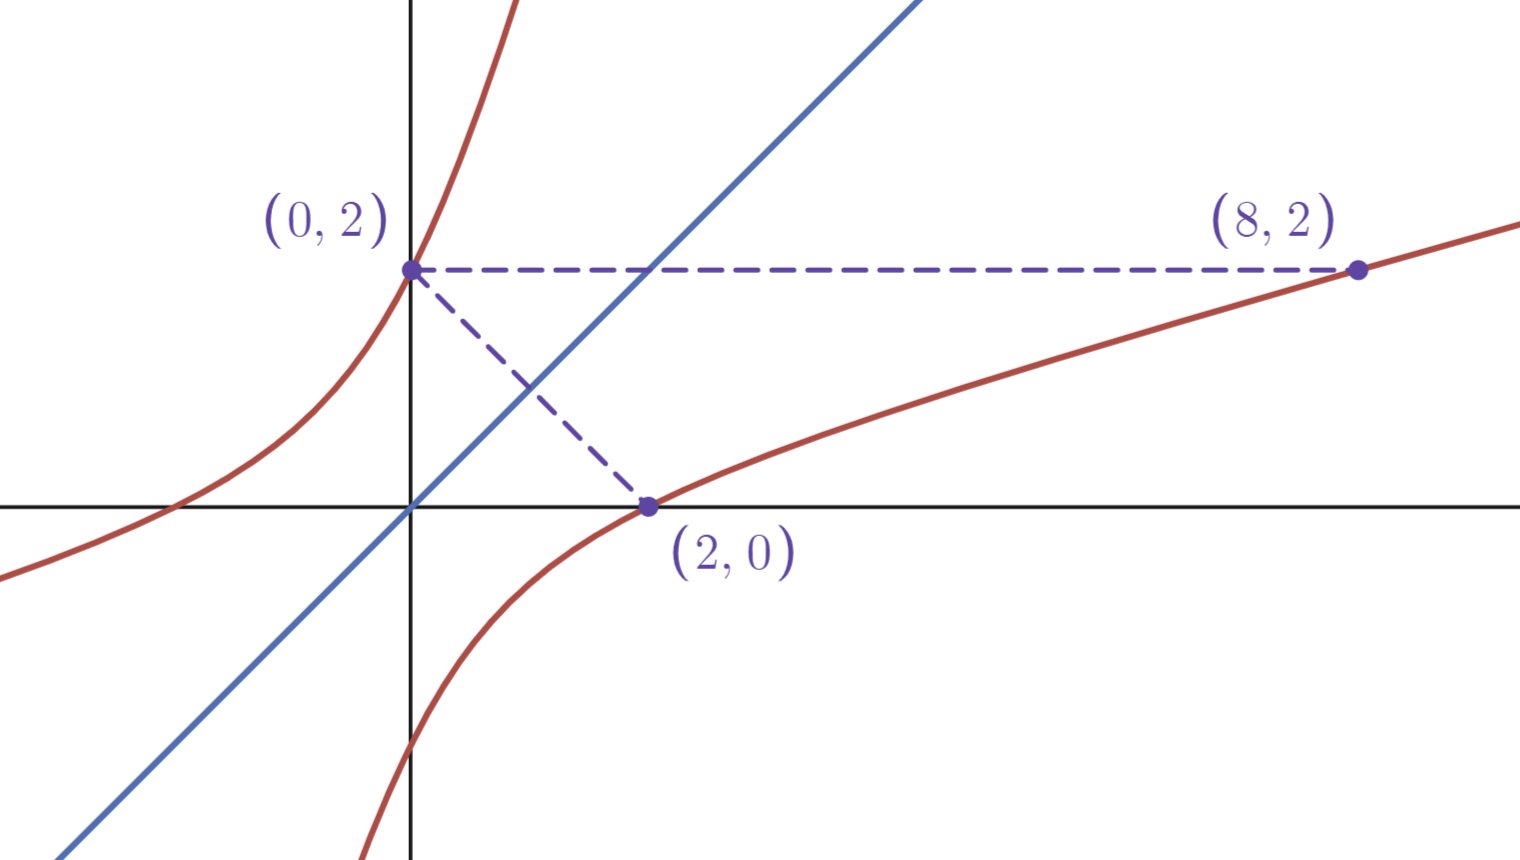
\includegraphics[scale=0.6]{imo_problem_hyperbola.png}\retTwo\par}
	\end{myIndent}
\end{myIndent}

\pracOne\mySepTwo

This is a complete tangent unrelated to the class but I can't help but want to look into it briefly. Any curve graphed by the equation $Ax^2 + By^2 + Cxy + Dx + Ey = F$ in the $xy$-plane is called a \udefine{conic}. Importantly, if $C = 0$ then we already know from high school precalculus how to tell if the graphed curve is an ellipse, parabola, or hyperbola. However, the $C$ coefficient complicates things. Is there a test we can do to still know what type of conic is graphed by our equation when $C \neq 0$?
\begin{myIndent}\pracTwo
	Let $f(x, y) = Ax^2 + By^2 + Cxy + Dx + Ey$ and consider any matrix $R = \left(\begin{matrix}
	r_1 & r_2 \\ r_3 & r_4
	\end{matrix}\right)$.\retTwo
	
	Then while it is messy, we can evaluate that:

	{\centering\begin{tabular}{l}
		$(f \circ R)(x, y) = (Ar_1^2 + Br_3^2 + Cr_1r_3)x^2 + (Ar_2^2 + Br_4^2 + Cr_2r_4)y^2$\\ [3pt]
		$\phantom{(f \circ R)(x, y) aaaaaa} + (2Ar_1r_2 + 2Br_3r_4 + Cr_1r_4 + Cr_2r_3)xy + (Dr_1 + Er_3)x$\\ [3pt]
		$\phantom{(f \circ R)(x, y) aaaaaa} + (Dr_2 + Er_4)y$
	\end{tabular}\retTwo\par}

	In particular, we care about when $R$ is a rotation matrix. So, we can assume there exists some $\theta$ such that:
	
	{\centering$R = \left(\begin{matrix}
	\cos(\theta) & -\sin(\theta) \\ \sin(\theta) & \cos(\theta)
	\end{matrix}\right)$.\retTwo\par}

	And now we want to fix $\theta$ such that:\\ [-10pt]

	{\centering\begin{tabular}{l}
		$0 = 2Ar_1r_2 + 2Br_3r_4 + Cr_1r_4 + Cr_2r_3$\\ [2pt]
		$\phantom{0} = -2A\cos(\theta)\sin(\theta) + 2B\sin(\theta)\cos(\theta) + C\cos^2(\theta) - C\sin^2(\theta)$\\ [2pt]
		$\phantom{0} = 2(B - A)\cos(\theta)\sin(\theta) + C(\cos^2(\theta) - \sin^2(\theta))$\\ [2pt]
		$\phantom{0} = (B - A)\sin(2\theta) + C\cos(2\theta)$.
	\end{tabular}\retTwo\par}

	Since we were originally motivated by the possibility that $B \neq 0$, for now I'm just going to assume $B \neq 0$. That way, we can explicitely calculate that $\theta = \frac{1}{2}\cot^{-1}(\frac{A - C}{B})$. And now by plugging that $\theta$ into our matrix $R$ we can find a rotation matrix such that $(f \circ R)(x, y)$ is another degree two polynomial but with $0$ for its $xy$ coefficient. And this proves that it is always possible to rotate our conic so that the $B$ term is $0$.\retTwo

	\mySepThree\newpage
	
	Unfortunately I don't have time to continue this tangent right now. I'll continue it later on \inLinkRap{page idk 1 reference}{page \_\_\_}.\retTwo
\end{myIndent}

\Hstatement\mySepTwo

\hTwo Before doing more 200a stuff, I unfortunately need to quickly do the rest of my math 220a homework since it is due in a few hours. So here it is:\retTwo

\Hstatement\blab{Exercise II.2.4:} Prove that if $\{D_j : j \in J\}$ is a collection of connected subsets of $X$ and if for each $j$ and $k$ in $J$ we have $D_j \cap D_k \neq \emptyset$, then $D \coloneqq \bigcup_{j \in J} D_j$ is connected.

\begin{myIndent}\HexOne
	Let $A$ be a set that is open and closed in $D$. Then we know that $A \cap D_j$ is both open and closed in the subspace topology of $D_j$. And since $D_j$ is connected, this means that either $A \cap D_j = \emptyset$ or $A \cap D_j = D_j$ for all $j \in J$.\retTwo

	Now suppose that $A \neq D$. That way, we know there is some $x \in D$ such that $x \notin A$. But then in turn there is some $k \in J$ such that $x \in D_k - A$. So, we know that $A \cap D_k = \emptyset$. And  since $D_j \cap D_k \neq \emptyset$ for all $j \in J$, we know that for each $j \in J$ there exists $y_j \in D_j$ such that $y_j \in D_j - A$. And hence, $A \cap D_j = \emptyset$ for all $j$. This shows $A = A \cap D = \emptyset$.\retTwo

	So since the only clopen sets in $D$ are $\emptyset$ and $D$, we know that $D$ is connected. $\blacksquare$\retTwo
\end{myIndent}

\blab{Exercise II.2.5:} Let $(X, d)$ be a metric space.
\begin{enumerate}
	\item[(a)] Show that if $F \subseteq X$ is closed and connected, then for every pair of points $a, b \in F$ and each $\varepsilon > 0$ there are points $z_0, \ldots, z_n$ in $F$ with $z_0 = a$, $z_n = b$, and $d(z_{k-1}, z_k) < \varepsilon$ for $1 \leq k \leq n$. Is the hypothesis that $F$ is closed needed?
	\begin{myIndent}\HexOne
		To start off, I don't know what Conway's obsession with writing the word "closed" is\\ because it is entirely unrelated to the proof which I imagine he intended for people to\\ write (considering I'm really just adapting Conway's proof for \inLinkRap{math 220a theorem II.2.3}{theorem II.2.3}).\retTwo

		Fix any $a \in F$ and $\varepsilon > 0$, and let $A$ be the set of $b \in F$ for which there exists\\ $z_0, \ldots, z_n \in F$ as in the statement of the exercise. Clearly $A \neq \emptyset$ since $a \in A$.\\ Meanwhile, we claim $A$ is clopen in $F$.\\ [-6pt]
		\begin{itemize}
			\item Suppose $b \in A$ and let $z_0, \ldots, z_{n}$ be a collection of points of $F$ with $a_0 = z_0$,\\ $b = z_{n}$ and $d(z_{k-1}, z_k) < \varepsilon$ for each $1 \leq k \leq n$. Then for any $w \in B_\varepsilon(b) \cap F$\\ (the ball of radius $\varepsilon$ centered at $b$ restricted to $F$), we know that $z_0, \ldots, z_n, w$ is\\ another collection of points of $F$ satisfying the conclusion of the exercise. So,\\ $B_\varepsilon(b) \cap F \subseteq A$. And this proves that $A$ is open in $F$.\retTwo
			
			\item In a similar vein, if $w \in F - A$, then we must have that $B_\varepsilon(w) \cap A = \emptyset$. So\\ $F - A$ is also open in $F$, and this shows that $A$ is closed in $F$.\retTwo
		\end{itemize}

		Now since $F$ is connected and $A \neq \emptyset$ is clopen, we know that $A = F$. $\blacksquare$ 
	\end{myIndent}

	\item[(b)] Show that even if $F$ is closed and satisfies the conclusion the previous statement, then we still don't necessarily have that $F$ is connected.
	\begin{myIndent}\HexOne
		We shall construct a "broken ladder" in $\mathbb{R}^2$. Specifically, define

		{\centering\fontsize{10}{12}\selectfont\begin{tabular}{l}
	$L \coloneqq \{(-1, y) \in \mathbb{R}^2 : y > 0\}\cup \{(+1, y) \in \mathbb{R}^2 : y > 0\} \cup \bigcup\limits_{k=1}^\infty\{(x, k) \in \mathbb{R}^2 : \frac{1}{k+1} \leq |x| \leq 1\}$.
		\end{tabular}\newpage\par}

		In order to see that $L$ is closed, consider that:

		{\centering\fontsize{10}{12}\selectfont \begin{tabular}{l}
	$\hspace{-3em}L^\comp = (((-\infty, -1) \cup (1, \infty)) \times \mathbb{R}) \cup (\mathbb{R} \times (-\infty, 0)) \cup \bigcup\limits_{k=1}^\infty ((-1, 1) \times (k-1, k)) \cup \bigcup\limits_{k=1}^\infty(\frac{-1}{k}, \frac{1}{k})\times (k-2, k)$. 
\end{tabular}\retTwo\par}

		Importantly, this shows that $L^\comp$ is a union of open sets. So $L^\comp$ is open and we in\\ turn know that $L$ is closed. Next note that $L$ is not connected. After all, note that\\ $A \coloneqq L \cap ((0, \infty) \times \mathbb{R}) = L \cap ([0, \infty) \times \mathbb{R})$ is both open and closed in $L$. That\\ said, $A \neq \emptyset$ and $A \neq L$.\retTwo
		
		\begin{tabular}{p{1in} p{5in}}
			\raisebox{-12em}{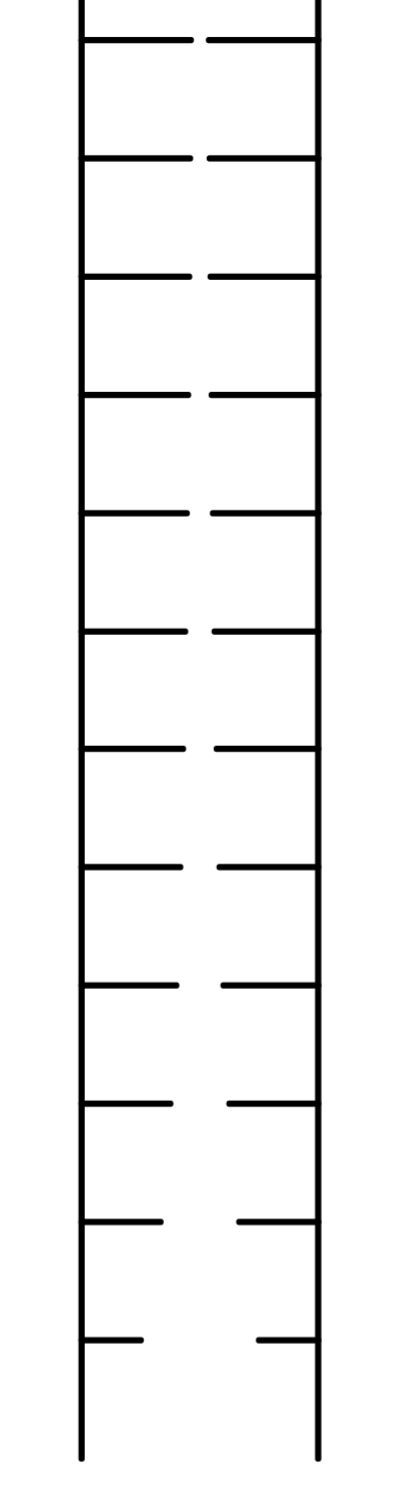
\includegraphics[scale=0.35]{Ladder_HW1_math220a.png}}
			&
			Finally note that $L$ does satisfy the conclusion of the problem\newline statement in part (a).  After all, $L \cap ((0, \infty))$ and $L \cap ((-\infty, 0))$ are\newline  easily checked to be the two connected components. So if $a, b$ are\newline in the same component, then we know from part (a) that a collection\newline $z_0, \ldots, z_n$ of points exists as described in the problem. Meanwhile\newline if $a$ and $b$ are in opposite components and $\varepsilon > 0$, then we know\newline there is some $k \in \mathbb{N}$ with $\frac{1}{k + 1} < \frac{1}{2}\varepsilon$. And then $(\frac{-1}{k+1}, k)$ and $(\frac{1}{k+1}, k)$\newline are two points in the opposite components that have distance $\varepsilon$ from\newline each other. $\blacksquare$\newline\phantom{.}\newline (Also see the drawing of $L$ to the side.)
		\end{tabular}
	\end{myIndent}
\end{enumerate}

\mySepTwo

\hTwo Ok back to math 200a stuff now.\retTwo

The kernel of a group action $a : G \times X \to X$ is the kernel of the induced group\\ homomorphism $G \to S_X$ (see the \inLinkRap{Alireza Theorem page 246}{theorem at the bottom of page 246}).\retTwo

Note that $g$ is in the kernel of the group action $(g, x) \mapsto g \cdot x$ precisely when for all $x \in X$ we have that $g \cdot x = x$. Also, the kernel $K$ of a group action is a normal subgroup and $G/K \hookrightarrow S_X$ (this arrow notation means that the induced homomorphism described in that theorem from $G/K$ to $S_X$ is injective / a monomorphism).\retTwo

Given a group action $G \curvearrowright X$ we define:
\begin{itemize}
	\item the \udefine{fixed set of $g$} to be $\Fix(g) = X^g \coloneqq \{x \in X : g \cdot x = x\}$ (where $g$ is fixed),
	\item the \udefine{stabilizer of $x$} to be $G_x \coloneqq \{g \in G : g \cdot x = x\}$ (where $x$ is fixed).\retTwo
\end{itemize}
	
\exTwo\hypertarget{Alireza lemma page 256}{\ul{Lemma:}} $G_x$ is a subgroup of $G$.
\begin{myIndent}\exThreeP
	Proof:\\ [-16pt]
	\begin{itemize}
		\item $1_g \cdot x = x \Longrightarrow 1 \in G_x$.
		\item Suppose $g_2 \in G_x$. Then $g_2 \cdot x = x \Longrightarrow g_2^{-1} \cdot (g_2 \cdot x) = g_2^{-1} \cdot x$. But note that\\ $g_2^{-1} \cdot (g_2 \cdot x) = (g_2^{-1}g_2) \cdot x = 1_G \cdot x = x$. So $g_2^{-1} \in G_x$.
		\item If $g_1, g_2 \in G_x$, then $(g_1g_2^{-1}) \cdot x = g_1 \cdot (g_2^{-1} \cdot x) = g_1 \cdot x = x$. So $g_1g_2^{-1} \in G_x$.\retTwo
	\end{itemize}

	This proves that $G_x$ is a subgroup of $G$. {\pracTwo(which by the way we shall denote as $G_x < G$).}\\ $\blacksquare$\newpage
\end{myIndent}

\exTwo\hypertarget{Alireza lemma page 257}{\ul{Lemma:}}\\ [-20pt]
\begin{itemize}
	\item[(a)] For all $g^\prime \in G$ we have that $\Fix(g^\prime g (g^\prime)^{-1}) = g^\prime \cdot \Fix(g) \coloneqq \{g^\prime \cdot x \in X : g \cdot x = x\}$.
	
	\begin{myIndent}\exThreeP
		Proof:
		
		{\centering\begin{tabular}{l}
			$x \in \Fix(g^\prime g (g^\prime)^{-1}) \Longleftrightarrow (g^\prime g (g^\prime)^{-1}) \cdot x = x$\\ [3pt]
			$\phantom{x \in \Fix(g^\prime g (g^\prime)^{-1})} \Longleftrightarrow g \cdot ((g^\prime)^{-1} \cdot x) = (g^\prime)^{-1} \cdot x$\\ [3pt]
			$\phantom{x \in \Fix(g^\prime g (g^\prime)^{-1})} \Longleftrightarrow (g^\prime)^{-1} \cdot x \in \Fix(g) \Longleftrightarrow x \in g^\prime \cdot \Fix(g)$.
		\end{tabular} \retTwo\par}
	\end{myIndent}

	\item[(b)] For all $g \in G$ we have that $G_{g \cdot x} = gG_xg^{-1}$
	
	\begin{myIndent}\exThreeP
		Proof:

		{\centering\begin{tabular}{l}
			$g^\prime \in G_{g \cdot x} \Longleftrightarrow g^\prime \cdot (g \cdot x) = g \cdot x$\\ [3pt]
			$\phantom{g^\prime \in G_{g \cdot x}} \Longleftrightarrow (g^{-1}g^\prime g) \cdot x = x \Longleftrightarrow g^{-1}g^\prime g \in G_x \Longleftrightarrow g^\prime \in gG_xg^{-1}$. $\blacksquare$
		\end{tabular}\retTwo\par}
	\end{myIndent}
\end{itemize}

\ul{Corollary:} Suppose $G \curvearrowright X$ and $|X| < \infty$. Then $g \mapsto |\Fix(g)|$ is a class function,\\ meaning that $|\Fix(g^\prime g (g^\prime)^{-1})| = |\Fix(g)|$ (or in other words $|\Fix(g)|$ is constant on\\ any given conjugate classes).

\begin{myIndent}\exThreeP
	Proof:\\
	$|\Fix(g^\prime g (g^\prime)^{-1})| = |g^\prime \cdot \Fix(g)|$ by the last lemma. And since $x \mapsto g^\prime \cdot x$ is an element\\ of $S_X$, we know that $|g^\prime \cdot \Fix(g)| = |\Fix(g)|$. $\blacksquare$\retTwo
\end{myIndent}

\hTwo The \udefine{$G$-orbit} of $x \in X$ is the set of all points in $X$ that are \udefine{$G$-similar} to $x$. Or to put into other words, we define $G \cdot x \coloneqq \{g \cdot x \in X : g \in G\}$ and say that $x^\prime$ is $G$-similar to $x$ if $x^\prime = g \cdot x \in G \cdot x$ for some $g \in G$. Also, in that case we denote $x^\prime \sim x$.\retTwo

\exTwo\ul{Lemma:} $\sim$ is an equivalence relation.
\begin{myIndent}\exThreeP
	Proof:\\ [-20pt]
	\begin{itemize}
		\item $x \sim x$ as $1_G \cdot x = x$.
		\item $x \sim y \Longrightarrow y \sim x$ as $x = g \cdot y \Longrightarrow g^{-1} \cdot x = y$.
		\item If $x \sim y$ and $y \sim z$ then let $g_1, g_2 \in G$ be such that $x = g_1 \cdot y$ and $y = g_2 \cdot z$. Then $x = (g_1g_2) \cdot z$. So $x \sim z$. $\blacksquare$\retTwo
	\end{itemize}
\end{myIndent}

\hTwo It's now clear that the $G$-orbit of $x$: $G \cdot x$, is the equivalence class of $x$ with respect to $\sim$. Thus, we define $X/G \coloneqq \{G \cdot x : x \in X\}$. Also note that $X/G$ is a partition of $X$. As a result, we know that $|X| = \hspace{-0.8em}\sum\limits_{G \cdot x \in X/G}\hspace{-0.8em} |G \cdot x|$.\retTwo

\exTwo\ul{Theorem (Orbit-stabilizer):} The map $G/G_x \to G \cdot x$ given by $gG_x \mapsto g \cdot x$ is a bijection. Hence $|G \cdot x| = [G : G_x]$ (where the latter is the number of left cosets of $G$ in $G_x$).
\begin{myIndent}\exThreeP
	Proof:\\
	We first show this map is well-defined. Suppose $g_1G_x = g_2G_x$. Then $g_2 = g_1h$ for some $g \in G_x$. And in turn $g_2 \cdot x = (g_1h) \cdot x = g_1 \cdot (h \cdot x) = g_1 \cdot x$.\retTwo

	Next we show injectivity. Assume $g_1 \cdot x = g_2 \cdot x$. Then $g_2^{-1} \cdot (g_1 \cdot x) = x$. So $g_2^{-1}g_1 \in G_x$. Or in other words, $g_1G_x = g_2G_x$.\retTwo

	Finally, surjectivity is obvious from the fact that $G \cdot x$ is the set of $y \in X$ such that there exists $g \in G$ with $g \cdot x = y$. $\blacksquare$\newpage
\end{myIndent}

\hTwo Note that $|G \cdot x| = 1$ iff $\forall g \in G,\gap g \cdot x = x$ iff $x \in \Fix(G)$ where:

{\centering$\Fix(G) = X^G \coloneqq \{x \in X : \forall g \in G,\gap g \cdot x = x\}$.\retTwo\par}

This leads to the equation:

{\centering$|X| = \hspace{-0.8em}\sum\limits_{\begin{smallmatrix}
	G \cdot x \in X/G \\ |G \cdot x| = 1
\end{smallmatrix}}\hspace{-0.8em} |G \cdot x| + 
\hspace{-0.8em}\sum\limits_{\begin{smallmatrix}
	G \cdot x \in X/G \\ |G \cdot x| > 1
\end{smallmatrix}}\hspace{-0.8em} |G \cdot x| = |\Fix(G)| + 
\hspace{-0.8em}\sum\limits_{\begin{smallmatrix}
	G \cdot x \in X/G \\ |G \cdot x| > 1
\end{smallmatrix}}\hspace{-0.8em} [G:G_x]$.\retTwo\par}

\Hstatement\mySepTwo

\hTwo I need to do the rest of the math 200a homework still. So I'm going to take a break from taking lecture notes to do the homework.\retTwo

\Hstatement\blab{Set 1 Problem 3:} Find the automorphism group of the Cayley graph of $\mathbb{Z}$ with respect to $\{-1, +1\}$.

\begin{myIndent}\HexOne
	To start off, note that $\{n, m\}$ is an edge of $\Cay(\mathbb{Z}, \{-1, 1\})$ iff $n - m = \pm 1$. This yields the infinite graph which I've attempted to draw below.\retTwo

	{\centering{\color{black}\raisebox{0em}{\tikz[scale=0.8,inner sep=4pt]{
		\tikzstyle{myCir}=[circle, fill, thick, color=black];
		\tikzstyle{myLine}=[thick, color=black];

		\node[myCir, label=above:$0$] (0) at (0, 0) {};
		\node[myCir, label=above:$1$] (1) at (2, 0) {} edge[myLine] (0);
		\node[myCir, label=above:$2$] (2) at (4, 0) {} edge[myLine] (1);
		\node[myCir, label=above:$3$] (3) at (6, 0) {} edge[myLine] (2);
		\node[myCir, label=above:$-1$] (-1) at (-2, 0) {} edge[myLine] (0);
		\node[myCir, label=above:$-2$] (-2) at (-4, 0) {} edge[myLine] (-1);
		\node[myCir, label=above:$-3$] (-3) at (-6, 0) {} edge[myLine] (-2);

		\node (+i) at (7.7, 0) {$\cdots$} edge[myLine] (3);
		\node (-i) at (-7.7, 0) {$\cdots$} edge[myLine] (-3);
	}}}\retTwo\par}

	Now from this graph it is clear that reversing the graph is a symmetry. Specifically, define $\tau(n) = -n$. Then $\tau(n) - \tau(m) = -n - (-m) = m-n = -(n-m)$. Hence, $n-m =\pm 1$ iff $\tau(n) - \tau(m) = \mp 1$ and we thus know that $\tau$ preserves the edges of our graph and is thus a symmetry.\retTwo

	Another obvious symmetry of our graph are index shifts. Specifically define $\sigma(n) = n + 1$. Then $\tau(n) - \tau(m) = n - m$ for all $n, m \in \mathbb{N}$ and it is thus obvious that $\tau$ preserves the edges of graph and is a symmetry.

	\begin{myDindent}\HexPPP
		I glossed over this point before but technically we also need to show $\sigma$ and $\tau$ are\\ bijections. To do this, just note that $\sigma^{-1}$ is given by $n \mapsto n-1$ and $\tau^{-1} = \tau$. So,\\ both maps are invertible.\retTwo
	\end{myDindent}

	Now we claim that every automorphism of $\Cay(\mathbb{Z}, \{-1, 1\})$ is some composition of $\tau$ and $\sigma$. To prove this, let $\theta$ be any arbitrary automorphism. We know that $\theta(0) = k$ for some $k \in \mathbb{Z}$. And in turn we have that $(\sigma^{-k} \circ \theta)(0) = 0$. Next note that $(\sigma^{-k} \circ \theta)(1)$ equals either $+1$ or $-1$. In the former case, we can trivially say that $\tau^0 \circ \sigma^{-k} \circ \theta$ fixes both $0$ and $1$. As for the latter case, since $\tau(0) = 0$ and $\tau(-1) = +1$, we can say that $\tau^{1} \circ \sigma^{-k} \circ \theta$ fixes both $0$ and $1$. Either way, this shows there exists a graph automorphism $\psi = \sigma^k \circ \tau^i$ (where $k \in \{\mathbb{Z}\}$ and $i \in \{0, 1\}$) such that $\psi^{-1} \circ \theta$ fixes both $0$ and $1$.\retTwo

	Observation: If $\phi \in \Aut(\Cay(\mathbb{Z}, \{-1, 1\}))$ with $\phi(0) = 0$ and $\phi(1) = 1$, then $\phi = \myId$.
	\begin{myIndent}\HexTwoP
		To prove this, we do induction separately on the positive integers and then on the negative integers.
		\begin{itemize}
			\item Suppose $n \geq 1$ and we've already shown that $\phi(k) = k$ for all $0 \leq k \leq n$. Then since $\phi$ is a graph automorphism, we must have that $\phi(n + 1) = \phi(n) \pm 1$. But since $\phi$ is a bijection and we already know that $\phi(n-1) = n-1 =\phi(n) - 1$, this means we can only have that $\phi(n+1) = \phi(n) + 1 = n + 1$. By induction this means that $\phi(n) = n$ for all $n \geq 0$.\retTwo
			
			\item Next suppose $n \leq 0$ and we've shown for all $k \geq n$ that $\phi(k) = k$. Then like before we must have that $\phi(n - 1) = \phi(n) \pm 1 = n \pm 1$ since $\phi$ is a graph automorphism. But since $\phi$ is a bijection and we already know $\phi(n + 1) = n + 1$,\newpage we can only have $\phi(n - 1) = n - 1$. By induction this means that $\phi(n) = n$ for all $n \in \mathbb{Z}$.\retTwo
		\end{itemize}
	\end{myIndent}

	Thus $\psi^{-1} \circ \theta = \myId$. Or in other words $\theta = \psi = \sigma^k \tau^i$ where $k \in \mathbb{Z}$ and $i \in \{0, 1\}$. This shows that $\Aut(\Cay(\mathbb{Z}, \{-1, 1\})) = \langle \sigma, \tau\rangle$.\retTwo

	Now the homework sheet specifically tells us to list out all the elements of the group of automorphisms. To do this, we need to show that $\sigma^{k_1} \circ \tau^{i_1} \neq \sigma^{k_2} \circ \tau^{i_2}$ if either $k_1 \neq k_2$ or $i_1 \neq i_2$. 
	\begin{myIndent}\HexTwoP
		To start off, note that $\sigma^{k_1}$ and $\sigma^{k_2}$ are easily checked to not equal each other when\\ $k_1 \neq k_2$. We merely note that $\sigma^{k_1}(0) = k_1 \neq k_2 = \sigma^{k_2}(0)$.\retTwo
		
		Also, it is easy to see that $\langle \sigma \rangle = \{\sigma^k : k \in \mathbb{Z}\}$ is a cyclic subgroup of our collection of symmetries and that $\tau$ is not in that subgroup. After all the only $k \in \mathbb{Z}$ such that $\sigma^k(0) = \tau(0)$ is $k = 0$. However, $\sigma^0(1) = 1 \neq -1 = \tau(1)$. It now follows that $\langle \sigma \rangle$ and $\langle \sigma \rangle \tau$ are two disjoint cosets which partition our collection of symmetries.\retTwo

		Finally, we need to show that if $k_1 \neq k_2$ then $\sigma^{k_1} \circ \tau \neq \sigma^{k_2} \circ \tau$. To do this, suppose $\sigma^{k_1} \circ \tau = \sigma^{k_2} \circ \tau$. Then by composing $\tau$ on the right side we get that $\sigma^{k_1} = \sigma^{k_2}$. And by prior work, we thus know that $k_1 = k_2$.\retTwo
	\end{myIndent}

	Thus $\Aut(\Cay(\mathbb{Z}, \{-1, 1\})) = \{\sigma^k \circ \tau^i : k \in \mathbb{Z} \text{ and } i \in \{0, 1\}\}$ and we know that the representation $\theta = \sigma^k \circ \tau^i$ is unique.\retTwo

	As for showing how to compose elements note that:

	{\centering $\tau \circ \sigma \circ \tau(n) = \tau \circ \sigma(-n) = \tau(-n + 1) = n - 1 = \sigma^{-1}(n)$.\retTwo\par}

	And since conjugation is a group automorphism, we know that:
	\begin{itemize}
		\item $(\sigma^m \circ \tau) \circ \sigma^n = \sigma^m \circ (\tau \circ \sigma^n \circ \tau) \circ \tau = \sigma^m \circ (\tau \circ \sigma \circ \tau)^n \circ \tau = \sigma^m \circ \sigma^{-n} \circ \tau$\\ [3pt]
		$\phantom{(\sigma^m \circ \tau) \circ \sigma^n = \sigma^m \circ (\tau \circ \sigma^n \circ \tau) \circ \tau = \sigma^m \circ (\tau \circ \sigma \circ \tau)^n \circ \tau} = \sigma^{m-n} \circ \tau$,\\

		\item $(\sigma^m \circ \tau) \circ (\sigma^n \circ \tau) = \sigma^m \circ (\tau \circ \sigma^n \circ \tau) = \sigma^m \circ (\tau \circ \sigma \circ \tau)^n = \sigma^m \circ \sigma^{-n} = \sigma^{m - n}$,\\

		\item $\sigma^m \circ (\sigma^n \circ \tau) = \sigma^{m + n} \circ \tau$ and $\sigma^m \circ \sigma^n = \sigma^{m + n}$. $\blacksquare$\retTwo
	\end{itemize}
\end{myIndent}

\blab{Set 1 Problem 2:} Suppose $G$ is a finite group and that for every positive integer $n$:\\ [-16pt]

{\center$|\{g \in G : g^n = e\}| \leq n$\\ [9pt]\par}

(where $e$ is the identity element of $G$). Use the following steps to prove that $G$ is a cyclic group.

\begin{enumerate}
	\item[(a)] Prove that if there is an element of order $d$ in $G$, then there are exactly $\phi(d)$ elements of\\ order $d$ in $G$ where $\phi(d)$ is the Euler $\phi$-function {\color{BrickRed}(where as a reminder $\phi(d)$ equals the\\ number of integers between $1$ and $d$ inclusive which are coprime to $d$)}.
	
	\begin{myIndent}\HexOne
		Suppose $g \in G$ with $o(g) = d$ and then consider the cyclic subgroup $\langle g \rangle \subseteq G$. We\\ [1pt] know that $o(g^k) = \frac{o(g)}{\gcd(o(g), k)} = \frac{d}{\gcd(d, k)} = d$ iff $\gcd(k, d) = 1$. So by considering $g^k$\\ for each $k \in \{1, \ldots, d\}$ with $\gcd(d, k) = d$ we get that there are at least $\phi(d)$\\ [3pt] distinct elements of $G$ with order $d$.\newpage

		That said, all $g^k$ where $k \in \{0, \ldots, d - 1\}$ are distinct elements of $\{g \in G : g^d = e\}$. And since $|\{g \in G : g^d = e\}| \leq d$, this proves that $h \in G$ can satisfy that $h^d = e$ only if $h = g^k$ for some integer $k$. And also because $h^d$ equaling $e$ is a necessary condition for us to have $o(h) = d$, we know that the $\phi(d)$ elements of $G$ we found before are the only elements of $G$ with order $d$.\retTwo
	\end{myIndent}
	
	\item[(b)] For every positive number $d$, let $\psi(d)$ be the number of elements of $G$ that have order $d$. Show that $\psi(d) \leq \phi(d)$ and that $\psi(d) \neq 0$ implies that $d \divides |G|$.
	
	\begin{myIndent}\HexOne
		We know that $\phi(d) \geq 1$ for all positive $d$ since $\gcd(1, d) = 1$. So, if $\psi(d) = 0$, then we trivially know that $\psi(d) \leq \phi(d)$. Meanwhile, if $\psi(d) > 0$ then we showed in part (a) that $\psi(d) = \phi(d)$. Hence in either case we have that $\psi(d) \leq \phi(d)$.\retTwo

		Also, the fact that $d \divides |G|$ if $\psi(d) \neq 0$ is just a result of Lagrange's theorem (since the order of any subgroup of $G$ must divides $|G|$ and $\phi(d) \neq 0$ implies there is a cyclic subgroup of $G$ with order $d$).\retTwo
	\end{myIndent}
	
	\item[(c)] Prove that $\psi(d) = \phi(d)$ if $d$ is a positive divisor of $|G|$. Deduce that $G$ is a cyclic group.
	
	\begin{myIndent}\HexOne
		Let $n = |G|$ and note that $\sum_{d \divides n} \psi(d) = n$ since every element of $G$ has some order dividing $n$. At the same time, it is a somewhat well known result that $\sum_{d \divides n} \phi(d) = n$ for all $n \in \mathbb{N}$.
		\begin{myIndent}\HexTwoP
			I can't find a proof of this result anywhere in my notes so I guess I'll prove it here.\retTwo

			Let $S = \{1, \ldots, n\}$ and define $S_d \coloneqq \{k \in S : \gcd(k, n) = d\}$ for each\\ $d$. Clearly, the $S_d$ form a partition of $S$ as we range over all the divisors\\ of $n$. Also note that there is a bijective correspondence between $S_d$ and\\ $E_{n/d} \coloneqq \{k \in \{1, \ldots, \frac{n}{d}\} : \gcd(k, \frac{n}{d}) = 1\}$.
			\begin{myIndent}\HexPPP
				Specifically note that $\gcd(m, n) = d \Longrightarrow \frac{m}{d}, \frac{n}{d} \in \mathbb{Z}$ with $\gcd(\frac{m}{d}, \frac{n}{d}) = 1$. And if we also have that $m \leq n$ then clearly $\frac{m}{d} \leq \frac{n}{d}$. So, $m \in S_d \Longrightarrow \frac{m}{d} \in E_{n/d}$. Meanwhile, if $\gcd(m, \frac{n}{d}) = 1$, then we know that $\gcd(dm, n) = d$. And also if $m \leq \frac{n}{d}$, then we know that $md \leq n$ Hence $m \in E_{n/d} \Longrightarrow dm \in S_d$. It now follows that the map $m \mapsto \frac{m}{d}$ is an invertible map from $S_d$ to $E_{n/d}$.\retTwo
			\end{myIndent}

			Now $|S_d| = |E_{n/d}| = \phi(\frac{n}{d})$. Also, we know that $n = |S| = \sum_{d \divides n} |S_d|$. So we have shown that $n = \sum_{d \divides n} \phi(\frac{n}{d}) = \sum_{d \divides n} \phi(d)$.\retTwo
		\end{myIndent}

		Since $\psi(d) \leq \phi(d)$ for all $d$, we thus have that:

		{\centering $n = \sum_{d \divides n} \psi(d) \leq \sum_{d \divides n} \phi(d) = n$.\retTwo\par}

		And this proves that $\sum_{d \divides n} \psi(d) = \sum_{d \divides n} \phi(d)$. Going even further, since\\ $0 \leq \psi(d) \leq \phi(d)$ for all $d$, the two sums can only equal if $\psi(d) = \phi(d)$ for all $d$ being summed over. In particular, we must have that $\phi(n) = \psi(n) \geq 1$. So, there is some element of order $n = |G|$ in $G$. This is equivalent to saying that $G$ is cyclic. $\blacksquare$\retTwo
	\end{myIndent}
\end{enumerate}

\blab{Set 1 Problem 1:} Suppose $G_1$ and $G_2$ are two groups. We say $G_1$ and $G_2$ are \udefine{algebraically\\ independent} if there are no proper normal subgroups $N_1$ and $N_2$ of $G_1$ and $G_2$ respectively\\ such that $G_1/N_1 \cong G_2/N_2$.\newpage
\begin{enumerate}
	\item[(a)] Prove that $G_1$ and $G_2$ are algebraically independent if and only if $G_1 \times G_2$ satisfies the following property: suppose $H$ is a subgroup of $G_1 \times G_2$ and the projection of $H$ to the $i$-th component is $G_i$ for $i = 1, 2$. Then $H = G_1 \times G_2$.
	\begin{myIndent}\HexOne
		\begin{myDindent}\exPPP
			As a reminder, the group $G_1 \times G_2$ is just the cartesian product\\ of the two groups equipped with the law of composition that\\ $(g_1, g_2)(g_1^\prime, g_2^\prime) = (g_1g_1^\prime, g_2g_2^\prime)$.\retTwo
		\end{myDindent}
		
		$(\Longrightarrow)$\\
		Suppose $G_1$ and $G_2$ are algebraically independent and then consider any subgroup $H \subseteq G_1 \times G_2$ such that $\pi_1(H) = G_1$ and $\pi_2(H) = G_2$ (where $\pi_1$ and $\pi_2$ are the projection maps). Also let $e_1$ and $e_2$ denote the identity elements of $G_1$ and $G_2$ respectively.\retTwo

		To start off, let $N_1 \coloneqq H \cap (\{e_1\} \times G_2)$ and $N_2 \coloneqq H \cap (G_1 \times \{e_2\})$. Then set $N_1^\prime \coloneqq \pi_2(N_1)$ and $N_2^\prime \coloneqq \pi_1(N_2)$. Both $N_1$ and $N_2$ are easily seen to be subgroups of $G_1 \times G_2$ as they are both intersections of groups. From there it also easy to see that $N_1^\prime$ and $N_2^\prime$ are subgroups of $G_2$ and $G_1$ respectively on account of being images of $N_2$ and $N_1$ via the homomorphisms $\pi_2$ and $\pi_1$. And of course there are obvious group isomorphisms showing that $N_1^\prime \cong N_1$ and $N_2^\prime \cong N_2$.
		\retTwo

		Our first big step is to show that $N_1^\prime$ and $N_2^\prime$ are normal subgroups (which in turn means that $G_1/N_2^\prime$ and $G_2/N_1^\prime$ are well-defined quotient groups).
		\begin{myIndent}\HexTwoP
			Suppose $g_1 \in N_2^\prime$ and let $g^\prime_1$ be any element of $G$. Since $\pi_1(H) = G_1$, we know\\ [2pt] there is some $g^\prime_2 \in G_2$ such that $(g^\prime_1, g^\prime_2) \in H$. And since $H$ is closed under\\ [2pt] inverses, we also know that $((g_1^\prime)^{-1}, (g_2^\prime)^{-1}) \in H$. Therefore $g^\prime_1 g (g^\prime_1)^{-1} \in N_2^\prime$\\ [2pt] since $(g^\prime_1 g (g^\prime_1)^{-1},  g^\prime_2 e_2 (g^\prime_2)^{-1}) = (g^\prime_1 g (g^\prime_1)^{-1}, e_2) \in H$. This proves that $N_2^\prime$ is\\ [2pt] normal in $G_1$. Analogous reasoning shows that $N_1^\prime$ is normal in $G_2$.\retTwo
		\end{myIndent}

		Next we define a group homomorphism $\phi$ from $G_1$ to $G_2/N_1^\prime$ as follows:

		{\centering Given any $g_1 \in G$, let $\phi(g_1) = g_2N_1^\prime$ where $(g_1, g_2) \in H$.   \retTwo\par}

		\begin{myIndent}\HexTwoP
			To show this is well defined, suppose $g_2, g_2^\prime \in G_2$ both satisfy that\\ [1pt] $(g_1, g_2) \in H$ and $(g_1, g_2^\prime) \in H$. Then $(e_1, g_2^{-1}g_2^\prime) \in H$, which in turns\\ [1pt] means that $g_2^{-1}g_2^\prime \in N_1^\prime$. This is equivalent to saying that $g_2^{-1} g_2^\prime N_1^\prime = N_1^\prime$\\ which in turn is equivalent to saying that $g_2^\prime N_1^\prime = g_2 N_1^\prime$.\retTwo

			Also, to see that $\phi$ is a homomorphism, suppose $(g_1, g_2), (g_1^\prime, g_2^\prime) \in H$.\\ [1pt] Then $(g_1g_1^\prime, g_2g_2^\prime) \in H$ and so $\phi(g_1g_1^\prime) = g_2g_2^\prime N_1^\prime$. But we also have that\\ [1pt] $\phi(g_1)\phi(g_2) = g_2N_1^\prime g_2^\prime N_1^\prime = g_2g_2^\prime N_1^\prime$. So $\phi(g_1g_2) = \phi(g_1)\phi(g_2)$.\retTwo
		\end{myIndent}

		Now we claim $\phi$ is surjective. After all, $\pi_2(H) = G_2$ so for all $g_2 \in G_2$ there exists\\ [1pt] $g_1 \in G_1$ such that $(g_1, g_2) \in H$. And then in turn $\phi(g_1) = g_2 N_1^\prime$. We also claim that\\ [1pt] the kernel of $\phi$ is $N_2^\prime$. After all, suppose $\phi(g_1) = N_1^\prime$. Then we know that there is some\\ [1pt] $g_2 \in G_2$ such that $(g_1, g_2) \in H$ and $(e_1, g_2) \in H$. But since $(e_1, g_2) \in H$, we also\\ [1pt] know that $(e_1, g_2^{-1}) \in H$, and thus $(e_1g_1, g_2^{-1}g_2) = (g_1, e_2) \in H$. So, $g_1 \in N_2^\prime$ and\\ [1pt] we've shown that $\ker(\phi) \subseteq N_2^\prime$. Going the other direction and showing $N_2^\prime \subseteq \ker(\phi)$\\ [1pt] is as simple as noting that $e_2N_1^\prime = N_1^\prime$.\newpage

		By the first isomorphism theorem, we are thus able to conclude that $\frac{G}{N_2^\prime} \cong \frac{G}{N_1^\prime}$.\retTwo

		{\color{red}I ran out of time so everything after this point is not being graded\dots\retTwo}

		Since $G_1$ and $G_2$ are algebraically independent, this implies that $N_2^\prime = G_1$ and\\ $N_1^\prime = G_2$. But now since $G_1 \times \{e_2\}$ and $\{e_1\} \times G_2$ are both contained in $H$ are\\ easily seen to together generate all of $G_1 \times G_2$, we know that $H = G_1 \times G_2$.\\ This proves the property in the problem statement.\retTwo

		$(\Longleftarrow)$\\
		Suppose $G_1$ and $G_2$ are not algebraically independent and let $N_1$ and $N_2$ be\\ proper normal subgroups of $G_1$ and $G_2$ such that $G_1 / N_1 \cong G_2 / N_2$. Then let\\ $\phi : G_1 / N_1 \to G_2 / N_2$ be a group isomorphism.\retTwo

		We define the set $H \coloneqq \{(g_1, g_2) \in G_1 \times G_2 : \phi(g_1N_1) = g_2N_2\}$ and claim that\\ this is a subgroup of $G_1 \times G_2$.
		\begin{myIndent}\HexTwoP
			\begin{itemize}
				\item Note that $(e_1, e_2) \in H$ since we must have that $\phi(N_1) = N_2$.\\ [-6pt]
				\item Suppose $(g_1, g_2) \in H$. Then $\phi(g_1 N_1) = g_2 N_2$. But note that:
				
				{\centering$N_2 = \phi(N_1) = \phi(g_1^{-1}g_1 N_1) = \phi(g_1^{-1} N_1)\phi(g_1 N_1) = \phi(g_1^{-1} N_1) g_2N_2$.\retTwo\par}

				Therefore $\phi(g_1^{-1}N_1) = (g_2N_2)^{-1} = g_2^{-1} N_2$ and we've shown that\\ $(g_1, g_2) \in H$.\\ [-6pt]

				\item Suppose $(g_1, g_2), (g_1^\prime, g_2^\prime) \in H$. Then we have that $\phi(g_1N_1) = g_2N_2$ and\\ $\phi(g_1^\prime N_1) = g_2^\prime N_2$. And since $\phi$ is a group homomorphism, we get that:
				
				{\centering $\phi(g_1g_1^\prime N_1) \phi(g_1 N_1)\phi(g_1^\prime N_1) = (g_2N_2)(g_2^\prime N_2) = g_2g_2^\prime N_2$. \retTwo\par}

				This shows that $(g_1g_1^\prime, g_2g_2^\prime) \in H$.\retTwo
			\end{itemize}
		\end{myIndent}

		Next observe that $\pi_1(H) = G_1$. After all, for any $g_1 \in G_1$ we can just pick\\ [1pt] $g_2 \in \phi(g_1 N)$ and then we'll know that $(g_1, g_2) \in H$. We also know that\\ [1pt] $\pi_2(H) = G_2$. After all, since $\phi$ is surjective, we know that for any $g_2 \in G_2$\\ [1pt] there exists a coset $g_1^\prime N_1 \in G_1/N_1$ such that $\phi(g_1^\prime N_1) = g_2N_2$. And now by\\ [1pt] just choosing any $g_1 \in g_1^\prime N_1$ we get that $(g_1, g_2) \in H$.\retTwo

		That said, $H \neq G_1 \times G_2$. To see this, just pick any $g_1 \in N_1$ and $g_2 \notin N_2$.\\ Then $\phi(g_1 N_1) \neq g_2N_2$ and we have that $(g_1, g_2) \notin H$. $\blacksquare$\retTwo
	\end{myIndent}
	
	\item[(b)] Suppose $G_1$ and $G_2$ are two finite groups and $\gcd(|G_1|, |G_2|) = 1$. Then $G_1$ and $G_2$ are algebraically independent.
	
	\begin{myIndent}\HexOne
		Let $H$ be any subgroup of $G_1 \times G_2$ such that $\pi_1(H) = G_1$ and $\pi_2(H) = G_2$.\\ [2pt] Since $\pi_1$ and $\pi_2$ are group homomorphisms from $G_1 \times G_2$ to $G_1$ and $G_2$ respectively,\\ [2pt] we know that both $|G_1| = |\pi_1(H)|$and $|G_2| = |\pi_2(H)|$ divide $|H|$. Hence,\\ [2pt] $\lcm(|G_1|, |G_2|)$ divides $|H|$. Meanwhile, we have by Lagrange's theorem that\\ [2pt] $|H|$ divides $|G_1 \times G_2| = |G_1||G_2|$.\retTwo

		But now because $\gcd(|G_1|, |G_2|) = 1$, we have that $\lcm(|G_1|, |G_2|) = |G_1||G_2|$ So, we must have $|H| = |G_1||G_2|$. And this proves that $H = G_1 \times G_2$.\newpage

		By part (a), we can now conclude that $G_1$ and $G_2$ are algebraically independent. $\blacksquare$
	\end{myIndent}
\end{enumerate}

\mySepTwo

\hTwo I'll continue with this class on \inLinkRap{math 200a lecture 4}{page 269}.\retTwo

\dispDate{10/5/2025}

I agreed to help present on a book (\textit{Ergodic Theory with a view towards Number Theory} by Einsiedler and Ward) this coming Wednesday. So today I'm going to be preparing for that.\retTwo

\ul{(Definition 2.1:)}
\begin{itemize}
	\item Let $(X, \mathcalli{B}, \mu)$ and $(Y, \mathcalli{C}, \nu)$ be probability spaces. A map $\phi : X \to Y$  is \udefine{measure preserving} if it is measurable and $\mu(\phi^{-1}(B)) = \nu(B)$ for all $B \in \mathcalli{C}$.
	
	\item If $T : (X, \mathcalli{B}, \mu) \to (X, \mathcalli{B}, \mu)$ is measure-preserving, then we call the measure space $(X, \mathcalli{B}, \mu)$ \udefine{$T$-invariant} and say that $(X, \mathcalli{B}, \mu, T)$ (which I will often shorthand as just $(X, T)$) is a \udefine{measure-preserving system}.\retTwo
\end{itemize} 

\exTwo\hypertarget{Einsiedler and Ward Theorem A.8}{\ul{Theorem A.8:}} Suppose $(X, \mathcalli{B}, \mu)$ and $(Y, \mathcalli{C}, \mu)$ are probability spaces and that $\mathcalli{E}$ is an\\ elementary family of sets that generates the $\sigma$-algebra $\mathcalli{C}$. Then a measurable map\\ $\phi: X \to Y$ is measure-preserving if and only if $\mu(\phi^{-1}(E)) = \nu(E)$ for all $E \in \mathcalli{E}$.
\begin{myIndent}\exThreeP
	$(\Longrightarrow)$\\
	This is trivial.\retTwo

	$(\Longleftarrow)$\\
	Let $\mathcalli{A}$ be the collection of all finite disjoint unions of elements in $\mathcalli{E}$, then recall from math 240a that $\mathcalli{A}$ is an algebra of sets and that by Carathéodory's theorem, any $\sigma$-finite measure on $\mathcalli{C}$ is uniquely determined by it's restriction to $\mathcalli{A}$.\retTwo

	Now importantly $\lambda: \mathcalli{C} \to [0, \infty]$ defined by $\lambda(C) = \mu(\phi^{-1}(C))$ is a well-defined\\ measure (You just need to note that $\phi^{-1}(\bigcup_{n \in \mathbb{N}} C_n) = \bigcup_{n \in \mathbb{N}} \phi^{-1}(C_n)$). And since $\mu$ is $\sigma$-\\finite, we know $\lambda$ is. So if $\lambda$ and $\nu$ agree on $\mathcalli{A}$, then they must agree on all of $\mathcalli{C}$. Also,\\ note that $\lambda$ and $\nu$'s values on $\mathcalli{A}$ are uniquely determined by their restrictions to $\mathcalli{E}$. So if\\ $\lambda|_\mathcalli{E} = \nu|_{\mathcalli{E}}$, we have that $\lambda = \nu$. $\blacksquare$\retTwo
	\begin{myIndent}\myComment
		As a side note: For this proof we didn't actually need $(X, \mathcalli{B}, \mu)$ and $(Y, \mathcalli{C}, \mu)$ to be probability measures. We just needed $\mu$ and $\nu$ to be $\sigma$-finite.\retTwo

		A typical application of this theorem will be that if we want to check that some map on $\mathbb{T} \coloneqq \mathbb{R} / \mathbb{Z}$ is measure-preserving then we only need to check cosets of half-intervals $[a, b)$ of $[0, 1)$.\retTwo
	\end{myIndent}
\end{myIndent}

\pracOne\mySepTwo

\hypertarget{Einsiedler and Ward trippy example}{Here} is a somewhat trippy example (to me):
\begin{myIndent}
	Consider $(\mathbb{T}, \mathcalli{B}_\mathbb{T})$ equipped with the Lebesgue measure $m$ and define $T_2 : \mathbb{T} \to \mathbb{T}$ by $T_2(t) = 2t \mMod{1}$. We claim that $T_2$ is a measure preserving map.\newpage

	\pracTwo
	Proof:\\
	Consider any half-interval $[a, b) \subseteq [0, 1)$. Then we have that:
	
	{\centering$T_2^{-1}([a, b)) = [\frac{a}{2}, \frac{b}{2}) \cup [\frac{a}{2} + \frac{1}{2}, \frac{b}{2} + \frac{1}{2})$.\retTwo\par}

	And hence $m(T_2^{-1}([a, b))) = \frac{b}{2} - \frac{a}{2} + (\frac{b}{2} + \frac{1}{2}) - (\frac{a}{2} + \frac{1}{2}) = b - a = m([a, b))$.\retTwo
\end{myIndent}

The reason I find this example a bit trippy is that if $b - a \leq \frac{1}{2}$ then we know that\\ $m(T_2([a, b))) = 2m([a, b))$. So I guess this example serves to illustrate that images of sets\\ with respect measure preserving maps don't need to have their measure preserved.\retTwo

To fully dispel my confusion, suppose $X$ and $Y$ are equipped with probability measures $\mu$ and $\nu$ respectively, $\phi: X \to Y$ is a measure preserving map, $x \in X$, and $y = \phi(x)$. The definition of measure preserving says that for all measurable sets $A \subseteq Y$ the probability that $y \in A$ is equal to the probability that $x \in \phi^{-1}(A)$. The last example however shows that if $B \subseteq X$ is measurable then the probability that $x \in B$ \textit{does not} have to equal the probability that $y \in \phi(B)$.\retTwo

That all said, we \textit{do} have that if $\phi$ is measure-preserving and bijective with a measurable inverse, then $\phi^{-1}$ is also measure preserving.
\begin{myIndent}\pracTwo
	This is because we then have for any measurable $B \subseteq X$ that:
	
	{\centering$\nu(\phi(B)) = \mu(\phi^{-1}(\phi(B))) = \mu(B)$.\retTwo\par}
\end{myIndent}

\mySepTwo

\hTwo If anyone in class asks, see my note on integrals of induced measures on \inLinkRap{Folland Proposition 10.1}{page 193.}\\ Otherwise I'll just state this without proof.
\begin{myIndent}
	\exTwo\ul{Lemma 2.6:} A measure $\mu$ on $X$ is $T$-invariant if and only if $\int f \df \mu = \int f \circ T \df \mu$ for all $f \in L^\infty(X, \mu)$. Moreover, if $\mu$ is $T$-invariant, then $\int f \df \mu = \int f \circ T \df \mu$ holds for all $f \in L^1(\mu, X)$.\retTwo
\end{myIndent}

\ul{(Definition 2.7:)} Let $(X, \mathcalli{B}_X, \mu, T)$ and $(Y, \mathcalli{B}_Y, \nu, S)$ be measure-preserving systems on probability spaces.
\begin{enumerate}
	\item The system $(Y, \mathcalli{B}_Y, \nu, S)$ is a \udefine{factor} of $(X, \mathcalli{B}_X, \mu, T)$ if there are sets $X^\prime \in \mathcalli{B}_X$ and\\ $Y^\prime \in \mathcalli{B}_Y$ with $\mu(X^\prime) = \nu(Y^\prime) = 1$,\phantom{a} $T(X^\prime) \subseteq X^\prime$, and $S(Y^\prime) \subseteq Y^\prime$, as well as a\\ measure-preserving map $\phi: X^\prime \to Y^\prime$ with $\phi \circ T(x) = S \circ \phi(x)$ for all $x \in X^\prime$. 
	
	\item If $\phi$ in the above definition has a measurable inverse, then we say $(Y, \mathcalli{B}_Y, \nu, S)$ is \udefine{isomorphic} to $(X, \mathcalli{B}_X, \mu, T)$.\retTwo
\end{enumerate}

Essentially if we let $\phi$ be undefined on a null set, then $(Y, \mathcalli{B}_Y, \nu, S)$ is a factor of\\ $(X, \mathcalli{B}_X, \mu, T)$ if there exists a function $\phi$ such that the diagram below commutes:

% https://q.uiver.app/#q=WzAsNCxbMCwwLCJYIl0sWzIsMCwiWCJdLFswLDIsIlkiXSxbMiwyLCJZIl0sWzAsMSwiVCJdLFsyLDMsIlMiLDJdLFswLDIsIlxccGhpIiwyXSxbMSwzLCJcXHBoaSJdXQ==
\[\begin{tikzcd}[sep=scriptsize]
	X && X \\
	\\
	Y && Y
	\arrow["T", from=1-1, to=1-3]
	\arrow["\phi"', from=1-1, to=3-1]
	\arrow["\phi", from=1-3, to=3-3]
	\arrow["S"', from=3-1, to=3-3]
\end{tikzcd}\]

\newpage

\begin{myIndent}\pracOne
	\begin{myClosureOne}{6}
		Here is my attempt at giving an example of a factor system where the two systems\\ are not isomorphic: (not in the book)\retTwo
		
		Let $\mathbb{T}^2$ and $\mathbb{T}$ be equipped with the Lebesgue measure, and let $\phi: \mathbb{T}^2 \to \mathbb{T}$ be\\ the projection of $\mathbb{T}^2$ onto $\mathbb{T}$. Then given any $(c_x, c_y) \in \mathbb{T}^2$ define $T: \mathbb{T}^2 \to \mathbb{T}$ by\\ $T(x, y) = (x + c_x, y + c_y)$ and $S: \mathbb{T} \to \mathbb{T}$ by $S(x) = x + c_x$.\retTwo

		Then it's clear that $T \circ \phi = \phi \circ S$, and you can also somewhat easily check that\\ $T$, $S$, and $\phi$ are measure-preserving.\\ [-4pt]
	\end{myClosureOne}\retTwo
\end{myIndent}

Here is a non-trivial example (from the book) of two systems that are isomorphic. To start off, let $\{0, 1\}$ be equipped with the discrete topology (turning it into a compact Hausdorff space) as well as the coin flip measure $\mu_{1/2, 1/2}$ on it's power set. 
\begin{myIndent}\myComment
	In other words $\mu_{1/2, 1/2}(\{0\}) = \mu_{1/2, 1/2}(\{1\}) = 1/2$.\retTwo
\end{myIndent}

Next let $X = \{0, 1\}^\mathbb{N}$ and equip $X$ with the (Radon) product measure $\mu = \prod_{n \in \mathbb{N}}\mu_{1/2,1/2}$. Then the \udefine{left shift map} $\sigma : X \to X$ defined by $\sigma(x_0, x_1, \ldots) = (x_1, x_2, \ldots)$ preserves $\mu$.

\begin{myIndent}\pracTwo
	Why?\\
	Since $\mu$ is defined on $\mathcalli{B}_X$ and is trivially $\sigma$-finite (since $\mu$ is a probability measure), we know by similar reasoning as in \inLinkRap{Einsiedler and Ward Theorem A.8}{theorem A.8} that $\sigma$ is measure preserving if and only if $\mu(\sigma^{-1}(U)) = \mu(U)$ for all open sets $U \subseteq \{0, 1\}^{\mathbb{N}}$ (in the product topology).\retTwo

	Now, Einsiedler and Ward call open sets in the product topology of $\{0, 1\}^\mathbb{N}$ \udefine{cylinder sets}. Specifically, $U \subseteq \{0, 1\}^\mathbb{N}$ is open iff there is a finite set $I \subseteq \mathbb{N}$ and a map $\mathbf{a}: I \to \{0, 1\}$ such that $U = \{(x_0, x_1, \ldots) \in X : x_j = \mathbf{a}(j) \text{ for all } j \in I\}$.

	\begin{myTindent}\begin{myTindent}
		(Also Einsiedler and Ward denote this set $I(\mathbf{a})$.)\retTwo
	\end{myTindent}\end{myTindent}

	With this notation in mind, let $I(\mathbf{a})$ be an open set in $\mathcalli{B}_X$. Then we clearly have that $\sigma^{-1}(I(\mathbf{a})) = I^\prime(\mathbf{a}^\prime)$ where $I^\prime = \{n + 1 : n \in I\}$ and and $\mathbf{a}^\prime: I^\prime \to \{0, 1\}$ is given by $\mathbf{a}^\prime(n) = \mathbf{a}(n - 1)$. But also note that:
	
	{\centering$\mu(\sigma^{-1}(I(\mathbf{a}))) = \mu(I^\prime(\mathbf{a}^\prime)) = (1/2)^{|I^\prime|} = (1/2)^{|I|} = \mu(I(\mathbf{a}))$\retTwo\par}
\end{myIndent}

Also note that the map $\phi: X \to \mathbb{T}$ given by $\phi(x_0, x_1, \ldots) = \sum_{n=0}^\infty \frac{x_n}{2^{n+1}}$ is measure-preserving from $(X, \mu)$ to $(\mathbb{T}, m)$ (where $m$ is the Lebesgue measure).
\begin{myIndent}\pracTwo
	Why?\\
	Note that the diadic rational numbers $\mathbb{Z}[\frac{1}{2}]$ are dense in the real numbers and include $0$\\ and $1$. And from there it is easy to see that the collection of cosets of half intervals\\ $[a, b) \subseteq [0, 1)$ such that $a, b \in \mathbb{Z}[\frac{1}{2}]$ is an elementary family generating $\mathcalli{B}_\mathbb{T}$. If we can\\ show that $\phi^{-1}([a, b)) \in \mathcalli{B}_X$ and that $\mu(\phi^{-1}([a, b))) = m([a, b))$ for all such half\\ intervals, we will have thus proven what we want.\retTwo

	Let $a$ and $b$ be diadic rationals with $a < b$. Then we know that there is some $n \in \mathbb{N}$ with the binary expansion of $a$ and $b$ being $a = 0.a_0a_1\cdots a_n\overline{11}$ and $b = 0.b_0b_1\cdots b_n\overline{00}$. So, for all $0 \leq k \leq n$ define:
	\begin{itemize}
		\item $A_k \coloneqq \{(x_0,x_1,\ldots) \in X : x_k > a_k \text{ and } x_i = a_i \text{ for all }i < k\}$,\newpage
		\item $B_k \coloneqq \{(x_0,x_1,\ldots) \in X : x_k < b_k \text{ and } x_i = b_i \text{ for all }i < k\}$.\retTwo
	\end{itemize}

	Also define:
	\begin{itemize}
		\item $A^\prime \coloneqq \{(x_0,x_1,\ldots) \in X : x_i = a_i \text{ for all }i \leq k\}$,
		\item $B^\prime \coloneqq \{(x_0,x_1,\ldots) \in X : x_i = b_i \text{ for all }i \leq k\}$.\retTwo
	\end{itemize}

	Then it is easy to see that $A^\prime, A_0, A_1, \ldots, A_n$ are all disjoint open sets in $X$. And similarly it is easy to see that $B^\prime, B_0, B_1, \ldots, B_n$ are all disjoint open sets in $X$. Plus:

	{\centering $\phi^{-1}([a, b)) = (A^\prime \cup \bigcup\limits_{k=0}^n A_k) \cap (B^\prime \cup \bigcup\limits_{k=0}^n B_k) - \{(b_0,b_1,\ldots, b_n, 1, 1, \ldots)\}$.\retTwo\par}

	This proves the first claim that $\phi$ is measurable.\retTwo

	As for actually calculating $\mu(\phi^{-1}([a, b)))$, let's now set $A = A^\prime \cup (\bigcup_{k=0}^n A_k)$ and\\ $B = B^\prime \cup (\bigcup_{k=0}^n B_k)$. Because $\{(b_0,b_1,\ldots, b_n, 1, 1, \ldots)\}$ is a null set, we can ignore\\ it. Also note that $A \cup B = X$. So we can evaluate that:\\ [-10pt]

	{\centering\begin{tabular}{l}
		$\mu(\phi^{-1}([a, b))) = \mu(A \cap B) = \mu(A) + \mu(B) - 1$\\ [6pt]

		$\phantom{\mu(\phi^{-1}([a, b))) = \mu(A \cap B)} = (\sum_{k=0}^n \mu(A_k)) + \mu(A^\prime) + (\sum_{k=0}^n \mu(B_k)) + \mu(B^\prime) - 1$.\\ [6pt]

		$\phantom{\mu(\phi^{-1}([a, b))) = \mu(A \cap B)} = (\sum_{k=0}^n \frac{1}{2^{k+1}}|a_k - 1|) + \frac{1}{2^{n+1}} + (\sum_{k=0}^n \frac{1}{2^{k+1}} b_k) + \frac{1}{2^{n+1}} - 1$.\\ [6pt]

		$\phantom{\mu(\phi^{-1}([a, b))) = \mu(A \cap B)} = (-\sum_{k=0}^n \frac{1}{2^{k+1}}(1 - a_k)) + b - 1$.\\ [6pt]

		$\phantom{\mu(\phi^{-1}([a, b))) = \mu(A \cap B)} = 1 - a + b - 1 $\\ [6pt]

		$\phantom{\mu(\phi^{-1}([a, b))) = \mu(A \cap B)} = b - a = m([a, b))$.\\ [6pt]
	\end{tabular}\retTwo\par}
\end{myIndent}

Finally, letting $T_2: \mathbb{T} \to \mathbb{T}$ be the map from \inLinkRap{Einsiedler and Ward trippy example}{earlier}, note that $\phi(\sigma(x)) = T_2(\phi(x))$ for all $x \in X$. And by restricting $\phi$ to the set $X^\prime \subseteq X$ of elements that aren't eventually just an infinite string of zeros or of ones, we then have that $\phi$ is a bijection to the set $\mathbb{T} - \mathbb{Z}[\frac{1}{2}]/\mathbb{Z}$. 

\begin{myIndent}\pracTwo
	As for how we know that $\mu(X^\prime) = 1$, note that the measure of all singletons of $X$ is $0$ and that $X - X^\prime$ is countable. So $\mu(X - X^\prime) = 0$.\retTwo
\end{myIndent}

At last this proves that $(X, \mathcalli{B}_X, \mu, \sigma)$ is isomorphic to $(\mathbb{T}, \mathcalli{B}_\mathbb{T}, m, T_2)$.

\begin{myIndent}\pracOne
	Note from 10/8/2025: Fuck I forgot to show that $\phi^{-1}$ is measurable.
\end{myIndent}
\mySepTwo

A measure-preserving transformation $T : X \to X$ on a probability space $(X, \mathcalli{B}, \mu)$ is \udefine{ergodic} if for any $B \in \mathcalli{B}$, $T^{-1}(B) = B \Longrightarrow \mu(B) = 0 \text{ or } \mu(B) = 1$.\retTwo

\begin{myIndent}\myComment
	By the way, I Googled it and apparently the term "ergodic" was coined by Boltzmann in the 1800s.\retTwo

	Also, FYI the notation $T^{-n}(B)$ just means the preimage $B$ with respect to $T^n$.\retTwo
\end{myIndent}

\exTwo\ul{Proposition 2.14:} The following are equivalent properties for a measure-preserving\\ transformation $T$ of $(X, \mathcalli{B}, \mu)$.\newpage
\begin{enumerate}
	\item[(1)] $T$ is ergodic.
	\item[(2)] For any $B \in \mathcalli{B}$ , $\mu(T^{-1}(B) \symdif B) = 0$ implies that $\mu(B) = 0$ or $\mu(B) = 1$.
	\item[(3)] For $A \in \mathcalli{B}$, $\mu(A) > 0$ implies that $\mu(\bigcup_{n=1}^\infty T^{-n}(A)) = 1$.
	\item[(4)] For $A, B \in \mathcalli{B}$, $\mu(A)\mu(B) > 0$ implies that there exists $n \geq 1$ with:
	
	{\centering$\mu(T^{-n}(A) \cup B) > 0$.\par} 
\end{enumerate}

\begin{myIndent}\exThreeP
	$(1 \Longrightarrow 2)$\\
	Assume $T$ is Ergodic and let $B$ be an \udefine{almost invariant} measurable set (meaning that\\ $\mu(T^{-1}(B) \symdif B) = 0)$. Then consider the set 
	
	{\centering$C = \limsup T^{-n}(B) = \bigcap\limits_{N = 0}^\infty \bigcup\limits_{n = N}^\infty T^{-n}(B)$.\retTwo\par}

	For any $N \geq 0$ we have that $B \symdif \bigcup_{n = N}^\infty T^{-n}(B) \subseteq \bigcup_{n = N}^\infty (B \symdif T^{-n}(B))$.

	\begin{myIndent}\exPPP
		Sanity check since I don't typically work with symmetric differences:
		
		{\centering$B \symdif \bigcup_{n = N}^\infty T^{-n}(B) = (B - \bigcup_{n = N}^\infty T^{-n}(B)) \cup ((\bigcup_{n = N}^\infty T^{-n}(B)) - B)$\retTwo\par}

		Then the result we want follows from the fact that:
		\begin{itemize}
			\item $(\bigcup_{n = N}^\infty T^{-n}(B)) - B = \bigcup_{n = N}^\infty (T^{-n}(B) - B)$,
			\item $B - \bigcup_{n = N}^\infty T^{-n}(B) \subseteq \bigcup_{n = N}^\infty (B - T^{-n}(B))$.\retTwo
		\end{itemize}
	\end{myIndent}

	But now note that $\mu(B \symdif T^{-n}(B)) = 0$ for all $n \geq 1$. This is because firstly,
	
	{\centering$B \symdif T^{-n}(B) \subseteq \bigcup_{i=0}^{n-1} (T^{-i}(B) \symdif T^{-(i + 1)}(B))$.\retTwo\par}

	\begin{myIndent}\exPPP
		Why?\\
		If $x \in T^{-n}(B) - B$, then we know there must exist some $i \in \{0, \ldots, n-1\}$ such that  $T^{i+1}(x) \in B$ but $T^i(x) \notin B$. Similarly, if $x \in B - T^{-n}(B)$, then we know there must exist some $i \in \{0, \ldots, n-1\}$ such that $T^i(x) \in B$ but $T^{i+1}(x) \notin B$.\retTwo
	\end{myIndent}

	And then since $T$ is measure-preserving we know for each $i$ that:
	
	{\centering$\mu(T^{-i}(B) \symdif T^{-(i + 1)}(B)) = \mu(B \symdif T^{-1}(B)) = 0$.\retTwo\par}

	This proves that for $C_n \coloneqq \bigcup_{n = N}^\infty T^{-n}(B)$ we have that $\mu(B \symdif C_n) = 0$. And in turn since the $C_n$ form a decreasing sequence with $C = \bigcap_{n \in \mathbb{N}} C_n$, we have by the monotonicity of measures that:

	{\center\begin{tabular}{l}
		$\mu(B \symdif C) = \mu((B - \bigcap_{n \in \mathbb{N}}C_n)) + \mu((\bigcap_{n \in \mathbb{N}}C_n) - B)$\\ [6pt]
		$\phantom{\mu(B \symdif C)} = \lim_{n \to \infty} \mu(B - C_n) + \lim_{n \to \infty}\mu(C_n - B) = \lim_{n \to \infty} \mu(B \symdif C_n) = 0$
	\end{tabular}\retTwo\par}

	This shows that $\mu(B \symdif C) = 0$. Or in other words, $\mu(B) = \mu(C)$. But now note that:

	{\centering $T^{-1}(C) = \bigcap\limits_{N = 0}^\infty \bigcup\limits_{n= N}^\infty T^{-(n + 1)}(B) = \bigcap\limits_{N = 0}^\infty \bigcup\limits_{n= N+1}^\infty T^{-n}(B) = C$ \retTwo\par}

	So by the ergodicity of $T$ we have that $\mu(C) = \mu(B)$ is either $0$ or $1$.\retTwo

	$(2 \Longrightarrow 3)$\\
	Let $A$ be a set with $\mu(A) > 0$ and let $B = \bigcup_{n=1}^\infty T^{-n}(A)$. Then:
	
	{\center$T^{-1}(B) = \bigcup_{n=2}^\infty T^{-n}(A) \subseteq B$.\newpage\par}
	
	Also, since $T$ is measure-preserving we know that $\mu(T^{-1}B) = \mu(B)$. Therefore\\ $\mu(T^{-1}(B) \symdif B) = 0$ and hence $\mu(B) = 0$ or $1$. But since $T^{-1}(A) \subseteq B$ with\\ $\mu(T^{-1}(A)) = \mu(A) > 0$, the former is impossible. So we must have that $\mu(B) = 1$.\retTwo

	$(3 \Longrightarrow 4)$\\
	Let $A$ and $B$ be sets of positive measure. Then $\mu(\bigcup_{n=1}^\infty T^{-n}(A)) = 1$. Hence:\\ [-10pt]
	
	{\center$0 < \mu(B) = \mu(B \cap \bigcup_{n=1}^\infty T^{-n}(A)) \leq \sum_{n=1}^\infty \mu(B \cap T^{-n}(A))$. \retTwo\par}

	And it follows that there must be some $n \geq 1$ with $\mu(B \cap T^{-n}(A)) > 0$.\retTwo

	$(4 \Longrightarrow 1)$\\
	Let $A$ be a set with $T^{-1}(A) = A$. Then for all $n \geq 1$ we have that:
	
	{\centering$0 = \mu(A \cap (X - A)) = \mu(T^{-n}(A) \cap (X - A))$.\retTwo\par}

	Hence to avoid contradicting (4), we must have that $\mu(A)\mu(X - A) = 0$. And that implies that either $\mu(A) = 0$ or $\mu(A) = 1$. $\blacksquare$\retTwo
\end{myIndent}

\hTwo Technically there is another equivalent condition that Einsiedler and Ward prove. However, I'm not going to continue with the proof cause I was just made aware that I read the wrong book. Oops.\retTwo

\mySepTwo

The real book I was supposed to read was \textit{Recurrence in Ergodic Theory and Combinatorial Number Theory} by Harry Furstenberg. I guess the key difference between this and the last text is that this will at first focus more on topological dynamics.\retTwo

A \udefine{dynamical system} is a compact metric space $X$ and a group (or semigroup) $G$ acting on $X$ by continuous transformations. We denote our system $(X, G)$. 
\begin{myIndent}\myComment
	Side note: a semigroup is a set and composition operator satisfying all the group axioms except possibly the identity and inverse axioms.\retTwo
\end{myIndent}

If $G = \mathbb{Z}$ or $\mathbb{N}$ we denote by $T$ the transformation on $X$ representing the action of $1 \in G$. We then denote our dynamical system as $(X, T)$ and call it a \udefine{cyclic system}.\retTwo

Let $T : X \to X$ be continuous. We say $x \in X$ is recurrent for $T$ (or for the dynamical system $(X, T)$) if for any neighborhood $V$ of $x$ there exists $n \geq 1$ with $T^n(x) \in V$. Or since $X$ is a metric space, $x$ is recurrent if there is an increasing sequence $(n_k)_{k \in \mathbb{N}} \subseteq \mathbb{N}$ such that $T^{n_k}(x) \to x$. {\pracOne(note from 10/8/2025: go \inLinkRap{Furstenberg confusion 1}{here} to see why these definitions are equivalent\dots)}\retTwo

\exTwo\ul{Claim:} If $X$ is a compact metric space and $T: X \to X$ is continuous, then there\\ always exists recurrent points. 
\begin{myIndent}\exThreeP
	Proof:\\
	Let $\mathcalli{F}$ be the family of nonempty closed subsets $Y \subseteq X$ with $T(Y) \subseteq Y$, and order $\mathcalli{F}$ by inclusion. By the finite intersection property, we know that $\bigcap_{\alpha \in A} Y_\alpha \neq \emptyset$ and is closed for all chains $\{Y_\alpha\}_{\alpha \in A} \subseteq \mathcalli{F}$. Hence by Zorn's lemma there is a minimal $Y_0 \neq \emptyset$ such $T(Y_0) \subseteq Y_0$. And we claim that each $x \in Y_0$ is recurrent for $T$.\newpage

	To show this, let $Q(x) = \overline{\{T^n (x) : n \geq 1\}}$. Then since $T(Y_0) \subseteq Y_0$, we know that\\ [1pt] $T^n(Y_0) \subseteq Y_0$ for all $n \geq 1$. And this proves that $Q(x) \subseteq \overline{Y_0} = Y_0$. At the same time\\ [1pt] note that $T(Q(X)) \subseteq Q(X)$. After all, if $y \in Q(x)$ and  $(n_k)_{k \in \mathbb{N}}$ is a sequence in $\mathbb{N}$ such\\ [1pt] that $T^{n_k}(x) \to y$, then because $T$ is continuous, we know that $T^{n_k + 1}(x) \to T(y)$.\retTwo

	But now by the minimality of $Y_0$ we have that $Q(X) = Y_0$. So, $x \in Q(x)$. $\blacksquare$\retTwo
\end{myIndent}

\hTwo Let $K$ be a compact metrized group, let $a \in K$, and define $T: K \to K$ by $T(x) = ax$. We then call the dynamical system $(K, T)$ a \udefine{Kronecker system}.

\begin{myIndent}\myComment
	As a side note, a \udefine{topological group} is a group equipped with a topology on which products and inverses are continuous. If that topology is also compact, we say we have a \udefine{compact group}.\retTwo
\end{myIndent}

\exTwo\ul{Theorem 1.2:} Every point in the space of a Kronecker system is recurrent.

\begin{myIndent}\exThreeP
	Proof:\\
	We know some point $x_0$ is recurrent. Now let $x$ be any point and write $x = x_0 u$. If $V$ is a neighborhood of $x$, then $Vu^{-1}$ is a neighborhood of $x_0$. And $a^n x_0 \in Vu^{-1}$ implies that $a^n(x_0 u) = a^n x \in V$. $\blacksquare$\retTwo
\end{myIndent}

\hTwo From now on, for the sake of shorthand I will write $gx$ instead of $T_g(x)$ when showing the continuous transformation associated with $g \in G$ acting on $x$. Also, for cyclic systems I'll just write $Tx$ instead of $T(x)$.\retTwo

Let $(X, G)$ and $(Y, G)$ be two dynamical systems with the same group/semigroup $G$\\ of operators. A \udefine{homomorphism} from $(X, G)$ to $(Y, G)$ is given by a continuous map\\ $\phi: X \to Y$ satisfying that $\phi(gx) = g\phi(x)$ for all $x \in X$ and $g \in G$.\retTwo

\ul{(Definition 1.3:)} A dynamical system $(Y, G)$ is a factor of the dynamical system $(X, G)$ if there is a homomorphism of the latter to the former given by a map $\phi$ of $X$ onto $Y$. In this case we also say that $(X, G)$ is an \udefine{extension} of $(Y, G)$.\retTwo

\exTwo\hypertarget{Furstenberg proposition 1.3}{\ul{Proposition 1.3:}} If $\phi$ determines a homomorphism of a cyclic system $(X, T_X)$ to $(Y, T_Y)$, and $x \in X$ is recurrent for $(X, T_X)$, then $\phi(x)$ is recurrent for $(Y, T_Y)$.
\begin{myIndent}\exThreeP
	Proof:\\
	Let $(n_k)_{k \in \mathbb{N}}$ be an increasing sequence in $\mathbb{N}$ and suppose that $T^{n_k}_X(x) \to x$. Then\\ because $\phi$ is continuous, we know $\phi(T^{n_k}_X(x)) \to \phi(x)$ as $k \to \infty$. But also note that\\ $\phi(T^{n_k}_X(x)) = T^{n_k}_Y\phi(x)$. So $T^{n_k}_Y\phi(x) \to \phi(x)$ as $k \to \infty$. $\blacksquare$\retTwo 
\end{myIndent}

\hTwo It's 3:30am and I need to go to sleep. I'll pick this particular subject up again probably tomorrow (technically today) late at night. \hypertarget{Ergodic reading group notes 1 back}{See} \inLinkRap{Ergodic reading group notes 2}{page 277}. \retTwo

\mySepTwo

\dispDate{10/6/2025}

\hypertarget{math 200a lecture 4}{\blect{Math 200a (lectures 4 \& 5):}}\newpage

\hypertarget{page 270 reference}{Here} is a small example of what we were talking about in the previous class:
\begin{myIndent}\hThree
	Suppose $G \curvearrowright G$ by conjugation and let us denote the orbit of $g$ as:

	{\centering$\Cl(g) \coloneqq \{g^\prime g (g^\prime)^{-1} : g^\prime \in G\}$.\retTwo\par}

	The stabilizer of $g$ is $\{g^\prime \in G : g^\prime g (g^\prime)^{-1} = g\} = \{g^\prime \in G : g^\prime g = g g^\prime\} \eqqcolon C_G(g)$.\\ We call this set (which is a subgroup via the \inLinkRap{Alireza lemma page 256}{lemma on page 256}) the \udefine{centralizer} of $g$.
	\begin{myIndent}\myComment
		Side note: $C_G(g)$ consists of all elements of $G$ that commute with $g$.\retTwo
	\end{myIndent}

	By the orbit-stabilizer theorem, we know $|\Cl(g)| = [G : C_G(g)]$. Also note that:

	{\centering$\Fix(G) = \{g^\prime \in G : \forall g \in G, \gap gg^\prime = g^\prime g\} \eqqcolon Z(G)$.\retTwo\par}

	\begin{myIndent}\myComment
		Side note: $Z(G)$ is called the \udefine{center} of $G$. Also, $Z(G) = \bigcap_{g \in G} C_G(g)$.\retTwo
	\end{myIndent}

	So $|G| = |Z(G)| + \hspace{-0.5em}\sum\limits_{\begin{smallmatrix}
		\Cl(g) \\ |\Cl(g)| > 1
	\end{smallmatrix}}\hspace{-0.5em}[G:C_G(g)]$.\retTwo
\end{myIndent}

\exTwo\ul{Cauchy-Frobenius Lemma:} Suppose $G$ is finite. Then:

{\centering$|X/G| = \AverageAst_{g \in G} |\Fix(g)| = \frac{1}{|G|}\sum\limits_{g \in G}|\Fix(g)|$\retTwo\par}

\begin{myIndent}\exThreeP
	Proof:\\
	Let $F \coloneqq \{(g, x) \in G \times X : g \cdot x = x\}$. Then clearly $|F| = \sum\limits_{g \in G} |\Fix(g)| = \sum\limits_{x \in X} |G_x|$.\retTwo

	But now recalling that $|G_{g\cdot x}| = |G_x|$ since $G_{g \cdot x} = gG_x g^{-1}$, we have that:

	{\center $\sum\limits_{x \in X} |G_x| = \hspace{-0.5em}\sum\limits_{G \cdot x \in X/G} \left( \sum\limits_{x^\prime \in G \cdot x} |G_{x^\prime}|\right) = \hspace{-0.5em}\sum\limits_{G \cdot x \in X/G} |G \cdot x| \cdot |G_x|$ \retTwo\par}

	Also from the orbit stabilizer theorem and Lagrange's theorem, we have that\\ $|G \cdot x| = [G : G_x] = \frac{|G|}{|G_x|}$. So $|G_x| = \frac{|G|}{|G \cdot x|}$. And hence:

	{\center$|F| = \hspace{-0.9em}\sum\limits_{G \cdot x \in X/G} \hspace{-0.9em} |G \cdot x| \cdot |G_x| =  \hspace{-0.9em}\sum\limits_{G \cdot x \in X/G} \hspace{-0.9em} |G \cdot x| \cdot \frac{|G|}{|G \cdot x|} = |G|\cdot|G/X|$ \retTwo\par}

	Thus $|G|\cdot|G/X| = \sum\limits_{g \in G} |\Fix(g)|$. $\blacksquare$\retTwo
\end{myIndent}

\pracOne\mySepTwo Suppose $G \curvearrowright X$. Then $G \curvearrowright X \times X$ by the action $g \cdot (x, y) = (g \cdot x, g \cdot y)$. What is $|(X \times X) / G|$?

\begin{myIndent}\pracTwo
	By the last lemma we have that:
	
	{\centering$|(X \times X) / G| = \frac{1}{|G|}\sum_{g \in G} |\{(x, y) \in X \times X : (g \cdot x, g \cdot y) = (x, y)\}|$.\retTwo\par}

	If $\Fix(g)$ refers to the fixed points of the action $G \curvearrowright X$, we thus have that:

	{\center\begin{tabular}{l}
		$|\{(x, y) \in X \times X : (g \cdot x, g \cdot y) = (x, y)\}|$\\ [4pt]
		$\phantom{aaaaaaaaaaaaaaaaaaa} = |\{(x, y) \in X \times X : x, y \in \Fix(g)\}| = |\Fix(g)|^2$
	\end{tabular} \retTwo\par}

	So $|(X \times X) / G| = \frac{1}{|G|}\sum_{g \in G} |\Fix(g)|^2$.\retTwo

	\myComment More generally, we can say that $|(\prod_{j=1}^n X) / G| = \frac{1}{|G|}\sum_{g \in G} |\Fix(g)|^n$.
\end{myIndent}
\mySepTwo\newpage

\hTwo \hypertarget{page 271 reference}{Let} $\Sub(G)$ denote the subgroups of $G$. Then $G \curvearrowright \Sub(G)$ via conjugation.
\begin{itemize}
	\item We denote $\Sub^{\lhd}(G)$ as the collection of normal subgroups of $G$. Note that\\ $(\Sub(G))^G = \Sub^{\lhd}(G)$.
	
	\item If $H \in \Sub(G)$, then the stabilizer of $H$ is equal to $N_G(H) \coloneqq \{g \in G : gHg^{-1} = H\}$. We call $N_G(H)$ the \udefine{normalizer} of $H$ in $G$.
	\begin{myIndent}\pracTwo
		Note that $H \lhd N_G(H)$ and that $N_G(H)$ is the largest subgroup of $G$ that has $H$ as a normal subgroup.\retTwo
	\end{myIndent}

	\item The $G$-orbit of $H$ consists of all subgroups of $G$ that are conjugate to $H$. The orbit-\\stabilizer theorem implies that the number of conjugates of a group $H$ is $[G : N_G(H)]$.\retTwo
\end{itemize}

\mySepTwo

\hTwo Suppose $p$ is prime and $G$ is a group with $|G| = p^k$ (where $k$ is an integer). In that case we say that $G$ is a \udefine{finite $p$-group}.\retTwo

\exTwo\hypertarget{Alireza theorem page 271}{\ul{Theorem:}} Suppose $G$ is a finite $p$-group and $G \curvearrowright X$ where $X$ is a finite set. Then\\ $|X| \equiv |X^G| \mMod{p}$.

\begin{myIndent}\exThreeP
	Proof:\\
	Note that if $H \lneqq G$ (meaning $H$ is a proper subgroup of $G$), then by Lagrange's theorem we have that $[G : H] \divides p^k$ and $[G : H] \neq 1$. Therefore, $[G : H] \equiv 0 \mMod{P}$. And in particular, we have that $[G : G_x] \equiv 0 \mMod{p}$ whenever $G_x \neq G$.\retTwo

	Now $|X^G| = |X| - \hspace{-0.8em}\sum\limits_{\begin{smallmatrix}
	G \cdot x \in X/G \\ |G \cdot x| > 1
\end{smallmatrix}}\hspace{-0.8em} [G : G_x]$.\retTwo And since $[G : G_x] \equiv 0 \mMod{p}$ for all $G_x$ with $[G : G_x] = |G \cdot x| > 1$ (so that $G \neq G_x$), we thus have that $|X^G| \equiv |X| \mMod{p}$. $\blacksquare$\retTwo
\end{myIndent}

\hypertarget{Cauchy's theorem page 271}{\ul{Theorem (Cauchy):}} Suppose $p \divides |G|$ where $p$ is prime. Then $\exists g \in G$ such that $o(g) = p$.
\begin{myIndent}\exThreeP
	Proof:\\
	We want to show that $|\{x \in G : x^p = 1\}| \equiv 0 \mMod{p}$.
	\begin{myIndent}\exPPP
		Why? Note that if $x \neq 1$ and $x^p = 1$, then we know that $o(x) = p$. Also, by showing that $|\{x \in G : x^p = 1\}| \equiv 0 \mMod{p}$ we know that there exists $x \in G - \{1\}$ with $x^p = 1$.\retTwo
	\end{myIndent}

	To do that, let $X \coloneqq \{(x_0, x_1, \ldots, x_{p-1}) \in G^p : x_0x_1\cdots x_{p-1} = 1 \}$. Then note that shifting an index is a symmetry of $X$. After all, if $1 = x_0x_1\cdots x_{p-1}$, then we have that:
	
	{\centering$1 = x_0^{-1}1x_0 = x_0^{-1}(x_0x_1\cdots x_{p-1})x_0 = x_1x_2\cdots x_{p-1}x_0$.\retTwo\par}

	So, $C_p \curvearrowright X$ where $C_p$ is the cyclic group of order $p$. And by the last theorem we have that $|X| \equiv |X^{C_p}| \mMod{p}$.\retTwo
	But now note that $X^{C_p} = \{(x, \ldots, x) \in G^p : xx\cdots x = 1\} = \{x \in G : x^p = 1\}$.\\ Also, we have that $|X| = |G|^{p-1}$ (since you can freely choose $x_0$ through $x_{p-2}$ and then $x_{p-1}$ must be whatever the inverse of $x_0 x_1 \cdots x_{p-2}$ is). And since $p \divides |G|$, we have that $|G|^{p-1} \equiv 0 \mMod{p}$. Hence, $|\{x \in G : x^p = 1\}| \equiv 0 \mMod{p}$. $\blacksquare$\newpage
\end{myIndent}

\hTwo $G$ is called a \udefine{$p$-group} if $o(g)$ is a power of $p$ for all $g \in G$.\retTwo

\exTwo\ul{Corollary:} If $G$ is finite and $p$ is prime, then $G$ is a $p$-group if and only if $|G| = p^n$ for some integer $n$. {\myComment(i.e. our new definition agrees with the old one)}
\begin{myIndent}\exThreeP
	$(\Longleftarrow)$\\
	This is just Lagrange's theorem.\retTwo

	$(\Longrightarrow)$\\
	If not, then there exists a prime factor $\ell \neq p$ such that $\ell \divides |G|$. Hence by Cauchy's theorem $G$ has an element of order $\ell$ (a contradiction). $\blacksquare$\retTwo
\end{myIndent}

\hypertarget{Alireza theorem center of p groups}{\ul{Proposition:}} Suppose $P$ is a finite $p$-group and $\{1\} \neq N \lhd P$. Then $Z(P) \cap N \neq \{1\}$.

\begin{myIndent}\exThreeP
	Proof:\\
	$P \curvearrowright N$ by conjugation. So $|N| \equiv |N^P| \mMod{p}$. Meanwhile note that:

	{\centering\begin{tabular}{l}
		$x \in N^P \Longleftrightarrow x \in N \text{ and } \forall g \in P,\gap g \cdot x = x$\\
		$\phantom{x \in N^P} \Longleftrightarrow x \in N \text{ and } \forall g \in P,\gap gxg^{-1} = x$\\
		$\phantom{x \in N^P} \Longleftrightarrow x \in N \text{ and } \forall g \in P,\gap gx = xg \Longleftrightarrow x \in Z(P) \cap N$.\\
	\end{tabular}\retTwo\par}

	So $|N| \equiv |Z(P) \cap N| \mMod{p}$. But finally note that $|N|$ divides $|P| = p^n$ for some $n$. But we also know by assumption that $|N| \neq \{1\}$. So, $|N| \equiv 0 \mMod{p}$ and we are done. $\blacksquare$\retTwo
\end{myIndent}

\hTwo\mySepTwo

The action $G \curvearrowright X$ is \udefine{transitive} if $|X/G| = 1$.\retTwo

\exTwo\ul{Proposition:} If $G \curvearrowright X$ transitively and $G, X$ are finite with $|X| > 1$, then there exists\\ $g \in G$ with $\Fix(g) = \emptyset$.

\begin{myIndent}\exThreeP
	Proof:\\
	Suppose $|\Fix(g)| \geq 1$ for all $g \in G$. Then:
	
	{\centering $|X/G| = \frac{1}{|G|}\sum_{g \in G} |\Fix(g)| \geq \frac{\Fix(1) + |G| - 1}{|G|} = \frac{|X| + |G| - 1}{|G|} > 1$. $\blacksquare$\retTwo\par}
\end{myIndent}

\ul{Corollary:} If $|G| < \infty$ and $H \lneqq G$, then $\bigcup_{g \in G} gHg^{-1} \neq G$.

\begin{myIndent}\exThreeP
	Proof:\\
	Consider $G \curvearrowright G/H$ by left translation. This is a transitive action. And since $[G : H] > 1$,\\ we know by the last proposition that there exists $g \in G$ such that $\Fix(g) = \emptyset$. Now notice that $g \cdot xH = xH \Longleftrightarrow x^{-1}gx \in H \Longleftrightarrow g \in xHx^{-1}$. So if $\Fix(g) = \emptyset$, then $g \notin \bigcup_{x \in G} xHx^{-1}$. $\blacksquare$\retTwo

	\pracOne
	\begin{myClosureOne}{6}
	\\ [-25pt] 
	Side note: the prior corollary does not hold if $|G| = \infty$. For example, consider\\ that $\GL_2(\mathbb{C}) = \bigcup_{x \in \GL_2(\mathbb{C})} xBx^{-1}$ where:
	
	{\centering$B \coloneqq \left\{\begin{bmatrix}
	a & b \\ 0 & c
	\end{bmatrix} \in \mathbb{C}^{2 \times 2} : a, b \neq 0\right\}$ is the set of all invertible\\ [-8pt]
	\phantom{aaaaaaaaaaaaaaaaaaaaaaaaaaaaaaaaaaa} upper triangular matrices.\retTwo\par}
	\end{myClosureOne}\retTwo
\end{myIndent}

\hTwo\mySepTwo\newpage

If $G$ is a group and $H < G$, then suppose $G \curvearrowright G/ H$ by left translations. What is the kernel of this action?
\begin{myIndent}\hThree
	Note that $g$ is in the kernel of the action iff $gxH = xH$ for all $x \in G$. And that happens iff $\forall x \in G, \gap g \in xHx^{-1}$ which happens iff $g \in \bigcap_{x \in G} xHx^{-1}$.\retTwo
\end{myIndent}

We call the kernel of the action above the \udefine{normal core} of $H$ in $G$, and denote it as\\ $\core_G(H)$ (or just $\core(H)$ if it's obvious what $G$ is).\retTwo

\exTwo\ul{Lemma:} $\core_G(H)$ is the largest normal subgroup of $G$ which is a subgroup of $H$ (i.e. $\core_G(H) \lhd G$, $\core_G(H) < H$, and if $N \lhd G$ with $N < H$ then $N < \core_G(H)$).

\begin{myIndent}\exThreeP
	By setting $x = 1$ we can see that $\core_G(H) \subseteq H$. Also, since $\core_G(H)$ is the kernel of the induced homomorphism $G \to S_{G/H}$, we know that $\core_G(H)$ is a normal subgroup.\retTwo

	Next suppose $N < H$ and $N \lhd G$. Since $N \subseteq H$, we know that $xNx^{-1} \subseteq xHx^{-1}$\\ for all $x \in G$. And then since $N \lhd G$, we know that $xNx^{-1} = N$ for all $x \in G$. So,\\ $N \subseteq xHx^{-1}$ for all $x \in G$. And this proves that $N \subseteq \bigcap_{x \in G} xHx^{-1} = \core_G(H)$. $\blacksquare$\retTwo
\end{myIndent}

\hTwo Also note that $H \lhd G$ if and only if $\core_G(H) = H$. With that we're now ready to prove the following proposition\dots\retTwo

\exTwo\ul{Proposition:} If $H < G$ and $[G : H] = p$ where $p$ is the smallest prime factor of $|G|$, then $H \lhd G$.
\begin{myIndent}\exThreeP
	Proof:\\
	Let $\phi: G \to S_p$ be the induced group homomorphism of the left translation action of $G$\\ [1pt] on $G/H$. Then note that $|\phi(G)|$ divides $\gcd(|G|, |S_p|) = \gcd(|G|, p!)$. But since $p$ is the\\ [1pt] smallest prime factor dividing $|G|$, we have that $\gcd(|G|, p !) = p$. So $|\phi(G)| \divides p$. Also note that $|\phi(G)| > 1$. After all, for any $g \notin H$ we have that $g \cdot 1H \neq 1H$ and thus $g$ doesn't\\ correspond to the identity permutation in $S_p$. So, $|\phi(G)| = p$.\retTwo

	But by Lagrange's theorem, we have that $[G: \core_G(H)] = |\phi(G)| = p$. And since $\core_G(H) \subseteq H$ and $[G : H] = p$, the only way this is possible is if $H = \core_G(H)$. So $H \lhd G$. $\blacksquare$\retTwo
\end{myIndent}

\hTwo\mySepTwo

\exTwo\ul{Theorem:} If $G$ is a finite group, $P < G$ is a $p$-group, and $p$ divides $[G : P]$, then\\ $p$ divides $[N_G(P) : P]$.
\begin{myIndent}\exThreeP
	Proof:\\
	$P \curvearrowright G/P$ by left-translations. Thus $|G/P| \equiv |(G/P)^P| \mMod{p}$. But note that:

	{\center\begin{tabular}{l}
		$xP \in (G/P)^P \Longleftrightarrow \forall g \in P,\gap g \cdot xP = xP$\\ [4pt]
		$\phantom{xP \in (G/P)^P} \Longleftrightarrow \forall g \in P,\gap g \in xPx^{-1} \Longleftrightarrow P \subseteq xPx^{-1}$
	\end{tabular} \retTwo\par}

	And since $|P| = |xPx^{-1}| < \infty$, we have that $P \subseteq xPx^{-1} \Longleftrightarrow P = xPx^{-1}$. And that happens iff $x \in N_G(P)$. So $|G/P| \equiv |N_G(P)/P| \mMod{p}$.\retTwo

	Next since $p$ divides $[G : P]$, we know that $0 \equiv |N_G(P)/P| \mMod{p}$. $\blacksquare$\retTwo
\end{myIndent}

\exTwo\ul{Corollary:} If $G$ is a finite $p$-group and $H \lneqq G$ then $H \lneqq N_G(H)$.\newpage
\begin{myIndent}\exThreeP
	Proof:\\
	If $|G| = p^n$ and $H \lneqq G$ then $H$ is a finite $p$-group and $p$ divides $[G : H]$. Then by the last theorem we have that $p$ divides $[N_G(H) : H]$. So, $H \lneqq N_G(H)$. $\blacksquare$\retTwo
\end{myIndent}

\ul{Sylow's 1st. Theorem:} Suppose $p^n$ divides $|G|$. Then there exists subgroups\\ $P_1 < P_2 < \cdots < P_n < G$ such that $|P_i| = p^i$ for all $1 \leq i \leq n$.
\begin{myIndent}\exThreeP
	Proof:\\
	We proceed by induction on $k$.\retTwo

	The base follows from Cauchy's theorem. Meanwhile suppose $p^{k+1}$ divides $|G|$ and we've already found subgroups $P_1 < \cdots < P_k < G$ such that $|P_i| = p^i$ for all $1 \leq i \leq k$. Then $p$ divides $[G : P_k]$, which means by two theorems ago that $p$ divides $[N_G(P_k) : P_k]$. And since $P_k \lhd N_G(P_k)$ we have that $N_G(P_k) / P_k$ is a well-defined group with $p \divides |N_G(P_k) / P_k|$.\retTwo

	By Cauchy's theorem and the correspondance theorem (the latter is in my math 100a paper notes), we thus know there is a subgroup $P_k < P_{k+1} < N_G(P_k)$ such that $P_{k+1}/P_k$ is a cyclic group of order $p$. And it follows that $|P_{k+1}| = |P_k| \cdot p = p^{k+1}$. $\blacksquare$\retTwo
\end{myIndent}

\hTwo We say that $\nu_p(|G|) = k$ if $p^k \divides |G|$ and $p^{k+1} \not\divides |G|$, and we call $\nu_p(|G|)$ the \udefine{$p$-valuation} of $G$.\retTwo

$P < G$ is called a \udefine{Sylow $p$-subgroup} if $|P| = p^{\nu_p(|G|)}$. Note that $P$ is a Sylow $p$-subgroup if and only if $P$ is a finite $p$-group and $p \not\divides\gap [G : P]$.\retTwo

Also, we let $\Syl_p(G)$ be the set of all Sylow $p$-subgroups of $G$.\retTwo

I'll continue with this class on \inLinkRap{math 200a lecture 6}{page 297}.

\mySepTwo

\dispDate{10/7/2025}

\hypertarget{math 220a lecture 3}{\blect{Complex Analysis Homework Assignment 2:}}\retTwo

Right now the class is still being boring and not really covering anything new. But I do still need to do homework for the class. So\dots\retTwo

\Hstatement\blab{Exercise II.3.1:} Prove the following:
\begin{itemize}
	\item[(a)] A set $A$ is closed iff it contains all its limits points.
	\item[(b)] If $A \subseteq X$, then $\overline{A} = A \cup \{x : x \text{ is a limit point of A}\}$.
\end{itemize}

\HexOne
\begin{myIndent}
	Ok actually frick whoever assigned this stupid problem. I'm not fricking type-setting\\ problems which are at the level of a first quarter undergrad analysis class. When will this\\ professor stop wasting everyone's time and actually get to the content that we're all paying out of our asses to learn? Hell! Math 200 and Math 240 started covering new content on the first day of class. This class is actual theft. Anyways here are my notes from math 240b:\newpage
\end{myIndent}

\hspace{-2em}\begin{tabular}{p{3.7in} p{3.7in}}
{\centering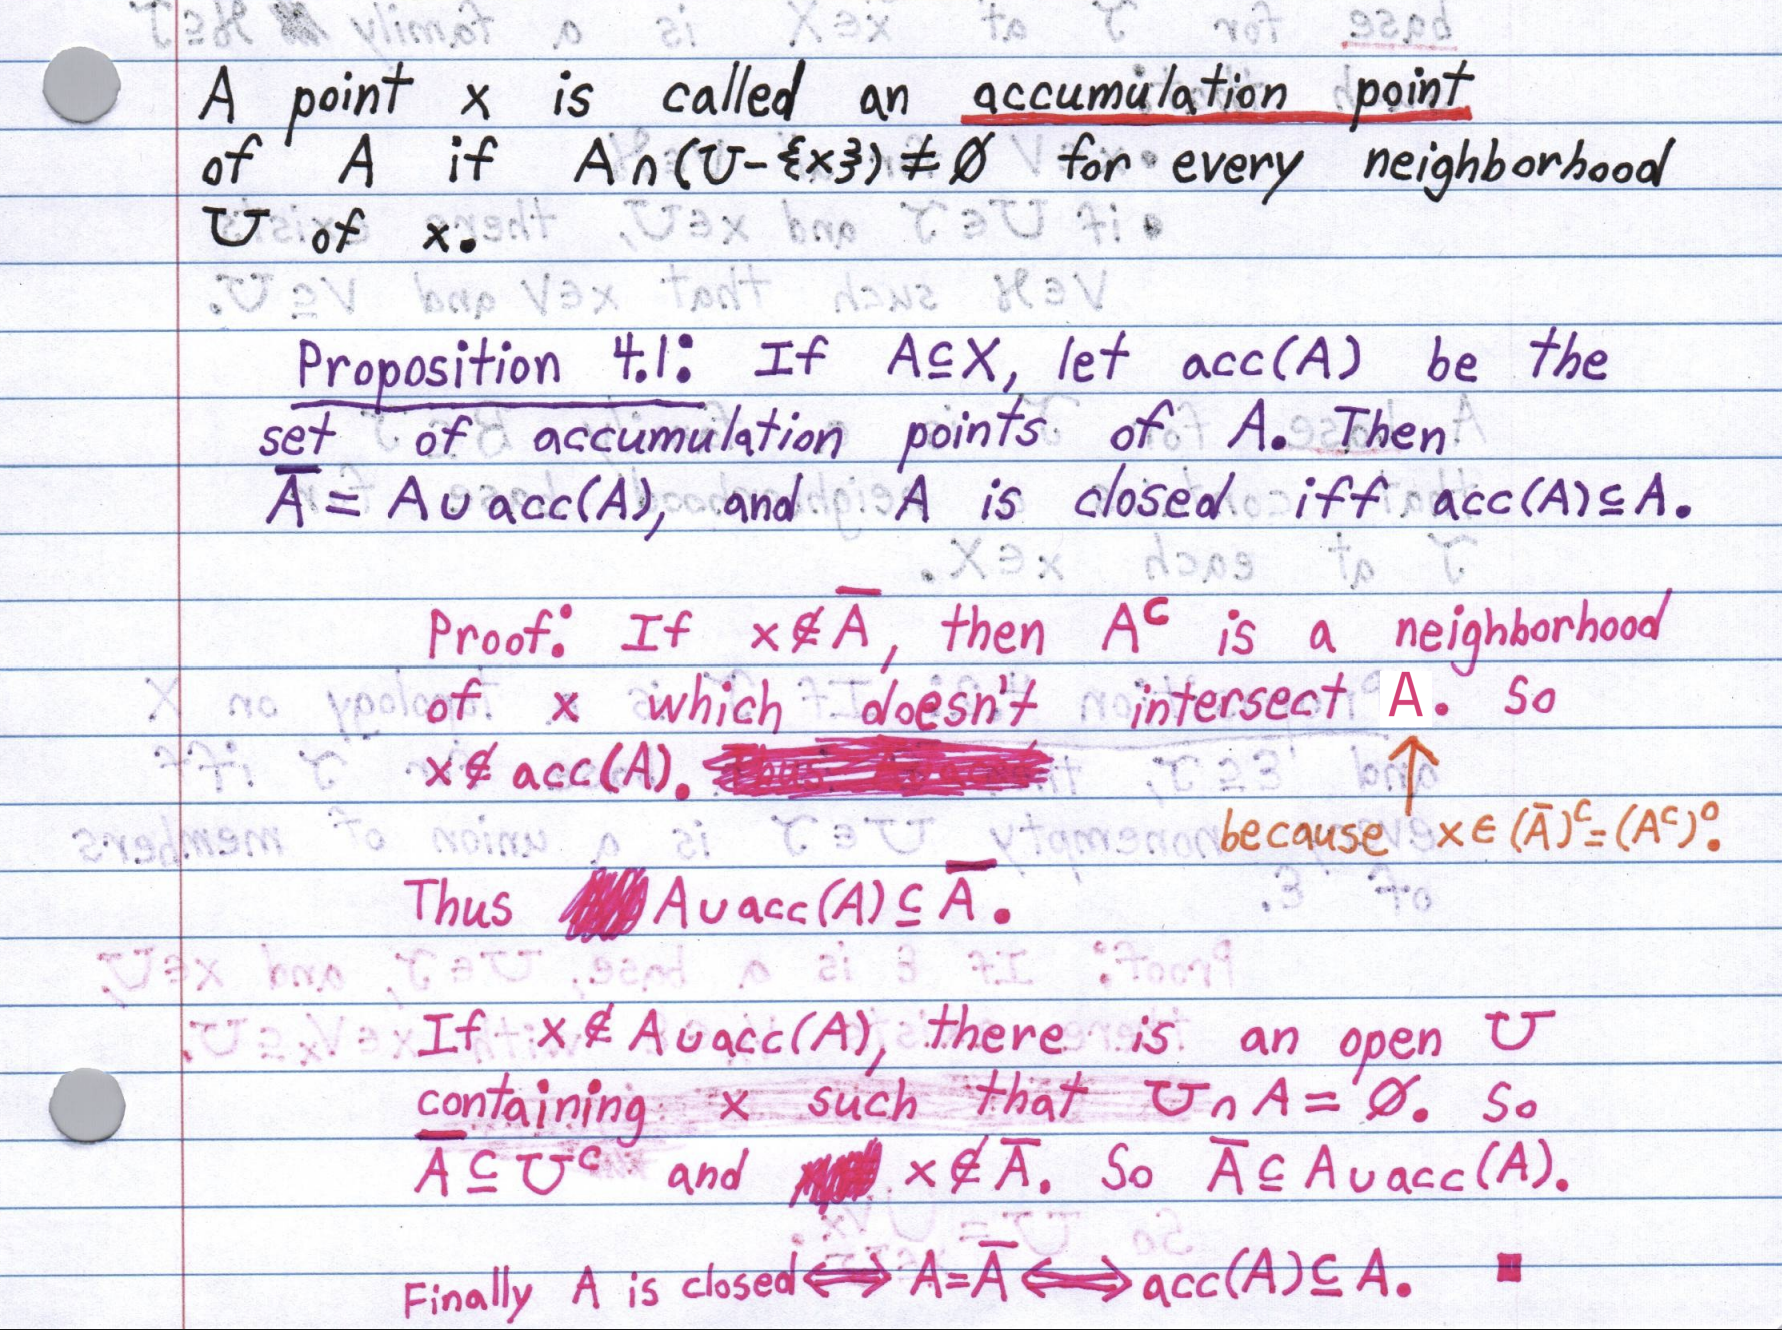
\includegraphics[scale=0.54]{HW2_1_math220a.png}\retTwo\par} & {\centering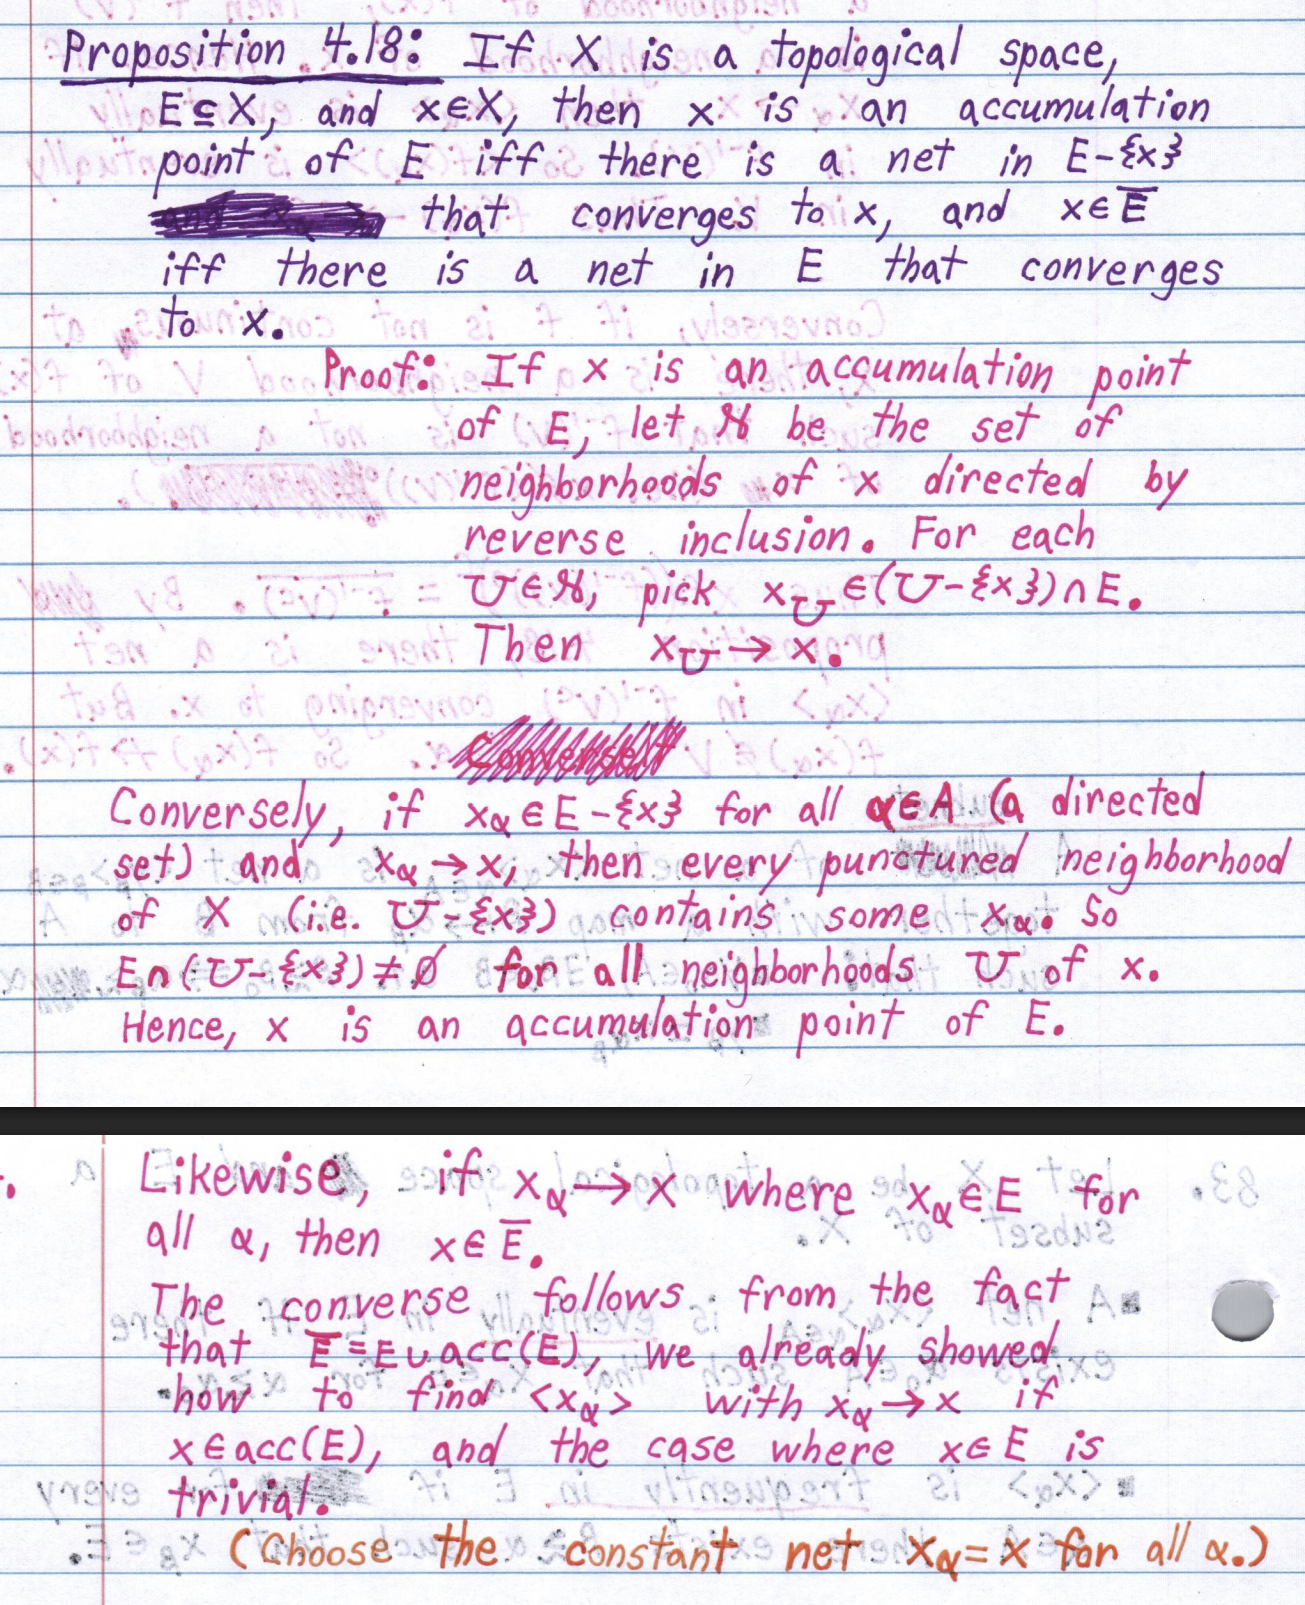
\includegraphics[scale=0.54]{HW2_2_math220a.png}\retTwo\par}
\end{tabular}\retTwo

\Hstatement\blab{Exercise II.3.4:} Let $z_n, z \in \mathbb{C}$ and let $d$ be the metric on $\mathbb{C}_\infty$. Then $|z_n - z| \to 0$ iff $d(z_n - z) \to 0$.

\begin{myIndent}\HexOne
	Recall that $d(z_n, z) = \frac{2|z_n - z|}{((|z_n|^2 + 1)(|z|^2 + 1))^{1/2}}$. Hence $d(x_n, z) \leq 2|z_n - z|$ and we have that $|z_n - z| \to 0 \Longrightarrow d(z_n - z) \to 0$.\retTwo
	
	On the other hand, if $\phi : \mathbb{C}_\infty \to S^2$ is the projection of the extended complex plane to\\ [1pt] the Riemann sphere, then by definition $d(z_n, z) \to 0$ iff $\phi(z_n) \to \phi(z)$ in $\mathbb{R}^3$. And since\\ [1pt] $\phi(z) \neq (0, 0, 1)$, there must exist some $-1 < C < 1$ and $N \in \mathbb{N}$ such that the third\\ [1pt] coordinates  of $\phi(z)$ and $\phi(z_n)$ are less than $C$ for all $n \geq N$. This translates to saying that:
	
	{\centering$\frac{|z|^2 - 1}{|z|^2 + 1}$ and $\frac{|z_n|^2 - 1}{|z_n|^2 + 1}$ are less than $C$ for all $n \geq N$.\retTwo\par}

	By quadratic formula this translate to saying that $|z_n|$ and $|z|$ are less than $D \coloneqq \frac{\sqrt{1 - C^2}}{1 - C}$\\ [-2pt] when $n \geq N$ So finally we may say that when $n \geq N$:

	{\center $|z_n - z| = \frac{1}{2}d(z_n, z)((|z_n|^2 + 1)(|z|^2 + 1))^{1/2} < \frac{1}{2}d(z_n, z)((D^2 + 1)(D^2 + 1))^{1/2}$ \retTwo\par}

	And now it's clear that $d(z_n - z) \to 0$ implies that $|z_n - z| \to 0$ as $n \to \infty$.\retTwo
\end{myIndent}

Also show that if $|z_n| \to \infty$, then $\{z_n\}_{n \in \mathbb{N}}$ is Cauchy in $\mathbb{C}_\infty$. 

\begin{myIndent}\HexOne
	To prove Cauchy-ness, it suffices to show $\{z_n\}_{n \in \mathbb{N}}$ converges to $\infty$. Fortunately, note that $d(z_n, \infty) - \frac{2}{(|z_n|^2 + 1)^{1/2}} \to 0$ as $|z_n| \to \infty$. So $z_n \to \infty$. $\blacksquare$\retTwo
\end{myIndent}

\blab{Exercise II.3.8:} Suppose $\{x_n\}_{n \in \mathbb{N}}$ is a Cauchy sequence in a metric space and $\{x_{n_k}\}_{k \in \mathbb{N}}$ is a convergent subsequence. Then $\{x_n\}$ is convergent.

\begin{myIndent}\HexOne
	Once again frick whoever is wasting all of our time with these stupid problems. Literally why I am wasting thousands of dollars to relearn content that any person getting into math grad school should already know.\retTwo

	Let $x$ be the limit of $\{x_{n_k}\}_{n \in \mathbb{N}}$ and pick any $\varepsilon > 0$.\newpage 
	
	Since $\{x_n\}_{n \in \mathbb{N}}$ is Cauchy there exists some $N \in \mathbb{N}$ such that $d(x_n, x_m) < \sfrac{\varepsilon}{2}$ for all\\ [1pt] $n, m \geq N$. Then because $x_{n_k} \to x$, we know there exists some $k \in \mathbb{N}$ such that\\ [1pt] $d(x_{n_k}, x) < \sfrac{\varepsilon}{2}$ and $n_k \geq N$. Thus, $d(x_n, x) \leq d(x_n, x_{n_k}) + d(x_{n_k}, x) < \varepsilon$ for all\\ [1pt] $n \geq N$. And this proves that $x_n \to x$ as $n \to \infty$. $\blacksquare$\retTwo
\end{myIndent}

\blab{Exercise II.4.1:} Prove that if every collection $\mathcalli{F}$ of closed subsets of $K$ with the finite intersection property has that $\bigcap_{F \in \mathcalli{F}} F \neq \emptyset$, then $K$ is compact.

\begin{myIndent}\HexOne
	Suppose $K$ is not compact and let $\{U_\alpha\}_{\alpha \in A}$ be an open cover of $K$ that has no finite\\ subcover. Then upon setting $F_\alpha = U_\alpha^\comp$ for all $\alpha \in A$ we have that $\{F_\alpha\}_{\alpha \in A}$ is a\\ collection of closed sets having the finite intersection property. After all, if there\\ were some $F_{\alpha_1}, \ldots, F_{\alpha_n}$ such that $\bigcap_{j=1}^n F_{\alpha_j} = \emptyset$ then that would imply that\\ [-1pt] $(\bigcap_{j=1}^n F_{\alpha_j})^\comp = \bigcup_{j=1}^n U_{\alpha_j} = K$. But that contradicts that $\{U_\alpha\}_{\alpha \in A}$ has no finite\\ [1pt] subcover of $K$.\retTwo

	At the same time though, $\bigcap_{\alpha \in A} F_\alpha = (\bigcup_{\alpha \in A} U_\alpha) = K^\comp = \emptyset$. So, we have found a\\ collection of closed sets with the finite intersection property whose intersection is\\ empty.  $\blacksquare$\retTwo
\end{myIndent}

\blab{Exercise II.4.4:} Show that the union of a finite number of compact sets is compact. 

\begin{myIndent}\HexOne
	Let $K_1, \ldots, K_n$ be a finite collection of compact sets and let $K$ be their union. Now if $\{U_\alpha\}_{\alpha \in A}$ is any open cover of $K$, then $\{U_\alpha\}_{\alpha \in A}$ is also an open cover of each $K_i$. So for each $i$ we can pick finitely many $U_{\alpha_j}$ covering each $K_i$. And by unioning the finitely many finite subcovers we get another finite subcover of all of $K$. $\blacksquare$\retTwo
\end{myIndent}

\blab{Exercise II.4.6:} Show that the closure of a totally bounded set is totally bounded.
\begin{myIndent}\HexOne
	Let $X$ be our metric space and suppose that $E \subseteq X$ is totally bounded. Then for any $\varepsilon > 0$ there are finitely many balls $B_1, \ldots, B_n$ of radius $\sfrac{\varepsilon}{2}$ covering $E$. And in turn the union of\\ [-1pt] the closures of those finitely many balls is a closed set containing $E$ and thus also $\overline{E}$. Finally, by expanding each of our balls to have radius $\varepsilon$ we now have a finite collection of balls of radius $\varepsilon$ covering $\overline{E}$.

	\begin{myIndent}\HexPPP
		Note to cover my bases:\\
		If $B_{\varepsilon/2}(x) \coloneqq \{y \in X : d(x, y) < \varepsilon/2\}$, then $\overline{B_{\varepsilon/2}(x)} \subseteq \{y \in X : d(x, y) \leq \varepsilon/2\}$ since the latter is easily checked to be closed set (it's complement is open by triangle inequality) which contains $B_{\varepsilon/2}(x)$. Also, $\{y \in X : d(x, y) \leq \varepsilon/2\} \subseteq \{y \in X : d(x, y) < \varepsilon\}$. $\blacksquare$\retTwo
	\end{myIndent}
\end{myIndent}

\blab{Exercise II.5.5:} Suppose $f: X \to \Omega$ is uniformly continuous (where $(\Omega, \rho)$ and $(X, d)$ are metric spaces). If $\{x_n\}_{n \in \mathbb{N}}$ is a Cauchy sequence in $X$ then $\{f(x_n)\}_{n \in \mathbb{N}}$ is a Cauchy sequence in $\Omega$.

\begin{myIndent}\HexOne
	Proof:\\
	For any $\varepsilon > 0$ pick $\delta > 0$ such that $\rho(f(x), f(y)) < \varepsilon$ whenever $d(x, y) < \varepsilon$. Since $\{x_n\}_{n \in \mathbb{N}}$ is a Cauchy sequence there exists some $N \in \mathbb{N}$ such that $d(x_n, x_m) < \delta$ for all $n, m \geq N$. And in turn $\rho(f(x_n), f(x_m)) < \varepsilon$ for all $n, m \geq N$. This proves that $\{f(x_n)\}_{n \in \mathbb{N}}$ is a Cauchy sequence in $\Omega$.\retTwo
\end{myIndent}

Does the prior statement still hold if $f$ is only assumed to be continuous but not\\ uniformly continuous.
\begin{myIndent}\HexOne
	No. For example, consider the sequence $\{\frac{1}{n}\}_{n \in \mathbb{N}}$ in $(0, \infty)$. This sequence is Cauchy since\\ for every $\varepsilon > 0$ we may choose some $N$ such that $\frac{1}{N} < \varepsilon$. And then for all $n, m \geq N$ we have that $|\frac{1}{n} - \frac{1}{m}| < \max(\frac{1}{n}, \frac{1}{m}) < \frac{1}{N} < \varepsilon$.\newpage

	Next let $f(x) = \frac{1}{x}$. To show that $f$ is continuous on $(0, \infty)$, note that both $1$ and $x$ are continuous on $(0, \infty)$. After all, just set $\delta = \varepsilon$ when doing the $\varepsilon$-$\delta$-proof. And since $x \neq 0$ on $(0, \infty)$, we have by proposition 5.5 in Conway that $\sfrac{1}{x}$ is continuous on $(0, \infty)$.\retTwo

	But now $\{\frac{1}{(1/n)}\}_{n \in \mathbb{N}}$ is not Cauchy. After all, for all $n,m \in \mathbb{N}$ with $n \neq m$ we have that:
	
	{\centering$|\frac{1}{(1/n)} - \frac{1}{(1/m)}| = |n - m| \geq 1$. $\blacksquare$\retTwo\par}
\end{myIndent}

\hTwo That's all my my math 220a homework for this week. Yay I'm done (finally). God I hope this class stops being a giant waste of money at some point. Anyways the next notes for this class will be on \inLinkRap{math 220a lecture 6}{page 294}.\retTwo

\mySepTwo

\hypertarget{Ergodic reading group notes 2}{My} next order of business for tonight is to continue taking notes for the reading group tomorrow. I'm picking up from \inLinkRap{Ergodic reading group notes 1 back}{here}.\retTwo

Let $(Y, T)$ be a dynamical system, $K$ be  a metrized compact group, and $\psi: Y \to K$ be a\\ continuous mapping. Then define $X = Y \times K$ and $T^\prime: X \to X$ by $T^\prime(y, k) = (Ty, \psi(y)k)$.\\ The resulting system is called a \udefine{group extension} or \udefine{skew product}  of $(Y, T)$ with $K$.

\begin{myIndent}\pracTwo
	Sanity check:
	\begin{enumerate}
		\item $T^\prime$ is a continuous map. After all, it's continuous iff its two output coordinates are individually continuous. And since we're already requiring $T$ and $\psi$ to be continuous and we know $(k_1, k_2) \mapsto k_1k_2$ is continuous from $K \times K$ to $K$, we can easily show both coordinates are continuous.\retTwo 
		
		\item If we define $\phi: X \to Y$ by $\phi(y, k) = y$, then $\phi$ is continuous (this is just a defining property of product topologies) and:
		
		{\centering$\phi(T^\prime(y, k)) = \phi(Ty, \psi(y)k) = Ty = T\phi(y, k)$.\retTwo\par}

		So, $\phi$ defines a homomorphism of $(X, T^\prime)$ to $(Y, T)$ and we've shown that $(X, T^\prime)$ does extend $(Y, T)$ by our prior definition.\retTwo
	\end{enumerate}
\end{myIndent}

\hTwo Note that in our above system, $X \curvearrowleft K$ by right translation. Specifically, for each $k^\prime \in K$ there exists a homeomorphism $R_{k^\prime} : X \to X$ given by $R_{k^\prime}(y, k) = (y, kk^\prime)$. Also, $R_k$ commutes with $T^\prime$ since:

{\centering $R_{k^\prime}(T^\prime(y, k)) = R_{k^\prime}(Ty, \phi(y)k) = (Ty, \phi(y)kk^\prime) = T^\prime(y, kk^\prime) = T^\prime(R_{k^\prime}(y, k))$ \retTwo\par}

Thus, each $R_{k^\prime}$ is an automorphism of the dynamical system $(X, T^\prime)$.


\begin{myIndent}\myComment 
	Side note:\\
	I think the author's choice to use right translations instead of left translations is really weird because it makes it so $R_{k_2}(R_{k_1}(y, k)) = (y, kk_1k_2) = R_{k_1k_2}(y, k)$. To fix this I would have instead set $T^\prime(y, k) = (Ty, k\psi(y))$ when defining the group extension, and then I'd have made $K \curvearrowright X$ by left translation. That way, we still have that $(X, T^\prime)$ is a dynamical system, $\phi$ is still a homomorphism from $(X, T^\prime)$ to $(Y, T)$, but now additionally we have that $R_{k_2} \circ R_{k_1} = R_{k_2k_1}$. Unfortunately, I don't want to confuse other presenters later on so I'll stick to the conventions of the book. :\lparen\newpage

Also just to be clear: I shall denote $X \curvearrowleft G$ instead of $G \curvearrowright X$ when $G$ is acting from the right on $X$ instead of from the left.\retTwo
\end{myIndent}

\pracOne\mySepTwo
Before moving on to the next theorem, I need to clear up some confusion and write a few theorems.\retTwo

Firstly, recall on \hypertarget{Furstenberg confusion 1}{page 268} when I said a point $x$ is recurrent for $(X, T)$ if for any\\ neighborhood $V$ of $x$ there exists $n \geq 1$ with $T^n x \in V$. And then I said that that is\\ equivalent to saying that there is some increasing sequence $(n_k)_{k \in \mathbb{N}} \subseteq \mathbb{N}$ such that\\ $T^{n_k}x \to x$. Why are these two definitions equivalent?

\begin{myIndent}\pracTwo
	$(\Longleftarrow)$\\
	This direction is obvious.\retTwo

	$(\Longrightarrow)$\\
	If $T^n(x) = x$ for some $n$, then we know that $T^{kn}(x) = x$ for all $k \in \mathbb{N}$ and then we trivially have that $T^{kn}(x) \to x$ as $k \to \infty$. Meanwhile, suppose $T^n(x) \neq x$ for any $n \in \mathbb{N}$ and let $\{U_k\}_{k \in \mathbb{N}}$ be a countable decreasing neighborhood base for $x \in X$. Then we may construct a subsequence $\{T^{n_k}\}_{k \in \mathbb{N}}$ converging to $k$ as follows:
	\begin{myIndent}
		To start off, just pick any $n_1 \in \mathbb{N}$ such that $T^{n_1}x \in U_1$. Then we proceed by recursive definition.\retTwo
		
		Suppose we have already chosen $n_1 < \cdots < n_k$ in $\mathbb{N}$ and that $T^{n_i}x \in V_{i}$ for all\\ $1 \leq i \leq k$.  If $X$ is Hausdorff (which it will always be if $X$ is a metric space), then we can find pairs of disjoint open sets $V_{j}, W_j \subseteq X$ for all $1 \leq j \leq n_{k}$ such that $x \in V_j$ and $T^{j}x \in W_j$. And by setting $V \coloneqq \bigcap_{j=1}^{n_k} V_j$ we have that $V$ is an open set containing $x$ such that $T^j x \notin V$ for all $1 \leq j \leq n_k$.\retTwo

		Now pick $m \geq k + 1$ such that $U_m \subseteq V$. Then by assumption, there is some $n_{k+1} \in \mathbb{N}$ such that $T^{n_{k+1}} x \in U_m$. And also we must have that $n_{k+1} > n_k$. $\blacksquare$\retTwo
	\end{myIndent}
\end{myIndent}

More generally, given a dynamical system $(X, T)$ and any $x \in X$, define the \udefine{forward orbit closure} of $x$ as $Q(x) \coloneqq \overline{\{T^n x : n \geq 1\}}$. Note that $x$ is recurrent for $(X, T)$ iff $x \in Q(x)$.\\ [1pt] Also, by slightly modified reasoning to before, we know $z \in Q(x)$ iff $z = T^nx$ for some $n$ or either there is some increasing sequence $\{n_k\}_{k \in \mathbb{N}}$ in $\mathbb{N}$ such that $T^{n_k} \to z$. \retTwo

\ul{Lemma A:} Let $(X, T)$ be a dynamical system and suppose that $y \in Q(x)$ and $z \in Q(y)$.\\ Then $z \in Q(x)$.
\begin{myIndent}\pracTwo
	Proof:\\
	It suffices to show $Q(y) \subseteq Q(x)$. Fortunately, if $y = T^n x$ for some $n \in \mathbb{N}$, then it's obvious that $Q(y) \subseteq Q(x)$. So we can now assume without loss of generality that there is some sequence $T^{n_i}x \to y$ as $i \to \infty$.\retTwo

	Next if $z = T^m y$ for some $m \in \mathbb{N}$, then it's clear that $T^m(T^{n_i}x) = T^{m + n_i}x \to z$ as $i \to \infty$, thus showing that $z \in Q(x)$. So, we may assume now that there is a sequence $T^{n_j}y \to z$ as $j \to \infty$.\retTwo

	Let $\{U_k\}_{k \in \mathbb{N}}$ be a countable decreasing neighborhood base for $z \in X$. We can construct a sequence $\{T^{n_k}x\}_{k \in \mathbb{N}}$ converging to $0$ as follows:\newpage
	\begin{myIndent}
		We'll want to keep track of subsequences of $\{n_{j(k)}\}_{k \in \mathbb{N}}$ and $\{n_{i(k)}\}_{n \in \mathbb{N}}$ of $\{n_j\}_{j \in \mathbb{N}}$ and $\{n_k\}_k \in \mathbb{N}$ respectively as we are constructing our actual desired sequence.\retTwo

		For any $k$ pick $j(k) \in \mathbb{N}$ such that $T^{n_{j(k)}}y \in U_k$ and $j(k) > j(k-1)$ (if $k > 1)$. Then set $V = (T^{n_j})^{-1}(U_k)$. Because $V$ is an open neighborhood of $y$, we know that there is some $I \in \mathbb{N}$ such that $T^{n_i}x  \in V$ whenever $i \geq I$. So pick $i(k)$ such that $T^{n_{i(k)}}x \in V$ and $i(k) > i(k-1)$ (if $k > 1$). Now $T^{n_{j(k)} + n_{i(k)}} x \in U_k$.\retTwo

		Doing this for all $K \in \mathbb{N}$, we get that $T^{n_{j(k)} + n_{i(k)}} x \to z$ as $k \to \infty$ and that\\ $\{n_{j(k)} + n_{i(k)}\}_{k \in \mathbb{N}}$ is increasing. $\blacksquare$\retTwo
	\end{myIndent}
\end{myIndent}

\ul{Lemma B:} Suppose $(X, T)$ is a dynamical system and $R$ is an automorphism of $(X, T)$\\ (meaning $R \circ T = T \circ R$ and $R : X \to X$ is continuous). Then for any $x \in X$ we have\\ that $R(Q(x)) \subseteq Q(Rx)$.

\begin{myIndent}\pracTwo
	Proof:\\
	Suppose $z \in Q(x)$. If $z = T^n x$ for some $n$, then $R(z) = R(T^n x) = T^n(Rx) \in Q(Rx)$. Otherwise, let $T^{n_k}x \to z$. Then $R(z) = \lim_{k \to \infty} R(T^{n_k}x) = \lim_{k \to \infty}T^{n_k}(Rx)$. So $R(z) \in Q(Rx)$ and we've shown that $R(Q(x)) \subseteq Q(Rx)$. $\blacksquare$\retTwo
\end{myIndent}

\ul{Lemma C:} Suppose $K$ is a compact metrized group and $k \in K$. Then the sequence $\{k^n\}_{n \in \mathbb{N}}$ has the identity $e$ of $K$ as a subsequential limit.

\begin{myIndent}\pracTwo
	Proof:\\
	We know that $(K, T)$ where $T(k^\prime) = k^\prime k$ is a Kronecker system. So $e \in K$ is recurrent and we know there is some increasing sequence $(n_i)_{i \in \mathbb{N}}$ of integers with $T^{n_i}e = k^{n_i - 1} \to e$ as $i \to \infty$. $\blacksquare$\retTwo
\end{myIndent}

I think before next week I will try to read up on topological groups some more cause I feel like I have a knowledge gap right now.\\
\mySepTwo

\exTwo\ul{Theorem 1.4:} If $y_0 \in Y$ is recurrent for $(Y, T)$ and $(X, T^\prime)$ is a skew extension of $(Y, T)$, then $(y_0, k_0)$ is a recurrent point of $(X, T^\prime)$ for all $k_0 \in K$.
\begin{myIndent}\exThreeP
	Proof:\\
	Let $e$ denote the identity of $K$. We shall show $(y_0, e)$ is a recurrent point of $(X, T)$ since it then follows from \inLinkRap{Furstenberg proposition 1.3}{proposition 1.3:} that each $R_{k_0}(y_0, e) = (y_0, k_0)$ is recurrent.\retTwo

	For any $x \in X$ let $Q(x) = \overline{\{(T^\prime)^n x : n \geq 1\}}$ denote the \udefine{forward orbit closure} of $x$. Then $x$ is recurrent for $(X, T^\prime)$ iff $x \in Q(x)$. Now since $y_0$ is recurrent for $(Y, T)$, there is some $k_1 \in K$ such that: $(y_0, k_1) \in Q(y_0, e)$.

	\begin{myIndent}\exPPP
		Why (since Furstenberg doesn't explain this)?\\ [4pt]
		Note that $(T^\prime)^n(y_0, e) = (T^n y_0, k^{(n)})$ where:
		
		{\centering$k^{(n)} = \phi(T^{n-1} y_0 ) \phi( T^{n-2} y_0) \cdots \phi(T y_0)\phi(y_0)$.\retTwo\par}

		Now because $y_0$ is recurrent for $(Y, T)$, we know that there is a subsequence\\ $\{T^{n_i} y\}_{i \in \mathbb{N}}$ such that $T^{n_i} y \to y$ as $i \to \infty$. And since $K$ is compact, we have that $\{k^{n_{i}}\}_{i \in \mathbb{N}}$ has a subsequential limit point $k_1$. And finally, by passing to another subsequence $\{n_{i_j}\}_{j \in \mathbb{N}}$ we get that $(T^\prime)^{n_{i_j}}(y_0, e) \to (y_0, k_1)$ as $j \to \infty$.\newpage
	\end{myIndent}

	But now note by induction that $(y_0, k_1^n) \in Q(y_0, e)$ for all $n \in \mathbb{N}$.

	\begin{myIndent}\exPPP
		Why?\\
		We know $(y_0, k_1) \in Q(y_0, e)$. Now by induction assume that $(y_0, k_1^n) \in Q(y_0, e)$. Then $(y_0, k_1^{n+1}) = R_{k_1}(y_0, k_1^n)  \in Q(R(y_0, e)) = Q(y_0, k_1)$ by lemma B. But we also have that $(y_0, k_1) \in Q(y_0, e)$. So $(y_0, k_1^{n+1}) \in Q(y_0, e)$ by lemma A.\retTwo
	\end{myIndent}

	In turn by lemma C we have that there is an increasing subsequence $\{n_j\}_{j \in \mathbb{N}}$ such that $(y_0, k^{n_j}) \to (y_0, e)$ as $j \to \infty$. And since $Q(y_0, e)$ is closed, we thus have shown that $(y_0, e) \in Q(y_0, e)$. $\blacksquare$\retTwo
\end{myIndent}

\hTwo By using the prior theorems we can inductively obtain examples of non-Kronecker\\ dynamical systems where every point is recurrent.\retTwo

For example, let $T : \mathbb{T}^2 \to \mathbb{T}^2$ be given by $T(\theta, \phi) = (\theta + a, \phi + 2\theta + a)$. Then $(\mathbb{T}^2, T)$ is a group extension of the Kronecker system $(\mathbb{T}, T^\prime)$ where $T^\prime \theta = \theta + a$ and $\psi(\theta) = 2\theta + a$. By theorems 1.2. and 1.4 we know that every point in $(\mathbb{T}^2, T)$ is recurrent.

In the prior system note that the orbit of $(0, 0) \in \mathbb{T}^2$ is:

{\centering\begin{tabular}{l}
	$(0, 0) \to (a, a) \to (2a, 4a) \to \cdots \to (na, n^2 a)$\\ [4pt]
	$\phantom{(0, 0) \to (a, a) \to (2a, 4a) \to \cdots} \to (na + a, n^2a + 2na + a) = ((n+1)a, (n^2 +2n + 1)a)$\\ [4pt]
	$\phantom{(0, 0) \to (a, a) \to (2a, 4a) \to \cdots \to (na + a, n^2a + 2na + a)} = ((n+1)a, (n+1)^2a) \to \cdots$ 
\end{tabular}\retTwo\par}

This leads to the following proposition:

\begin{myIndent}\exTwo
	\ul{Proposition 1.5:} For any $\alpha \in \mathbb{R}$ and $\varepsilon > 0$ we can solve the diophantine inequality $|\alpha n^2 - m| < \varepsilon$ (where $n > 0$).

	\begin{myIndent}\exThreeP
		Proof:\\
		We know there is some increasing sequence $\{n_k\}_{k \in \mathbb{N}}$ in $\mathbb{N}$ such that\\ $(n_k a, n_k^2 a) \to (0, 0) \in \mathbb{T}^2$. In particular, since $n_k^2 a \to 0 \in \mathbb{T}$ we know that\\ if $k$ is fixed large enough, then there exists $m \in \mathbb{N}$ such that $|n_k^2 - m| < \varepsilon$. $\blacksquare$\retTwo
	\end{myIndent}
\end{myIndent}

We can extend this to higher degree polynomials too. Let $p(x)$ be a polynomial of degree $d$ with real coefficients and write $p_d(x) \coloneqq p(x)$ as well as:

{\centering $p_{d-1}(x) \coloneqq p_d(x + 1) - p_d(x)$, $\phantom{a}p_{d-2}(x) \coloneqq p_{d-1}(x + 1) - p_{d-1}(x)$, etc. \retTwo\par}

Each $p_i(x)$ is of degree $i$. Let $\alpha$ be the constant $p_0(x)$. Then define a transformation\\ $T: \mathbb{T}^d \to \mathbb{T}^d$ by $T(\theta_1, \theta_2, \theta_3 \ldots, \theta_d) \coloneqq (\theta_1 + \alpha, \theta_2 + \theta_1, \theta_3 + \theta_2, \ldots, \theta_d - \theta_{d-1})$.

\begin{myIndent}\pracTwo
	By induction, we can see that this is a group extension of a dynamical system on the $(d-1)$-torus which in turn is a group extension of a dynamical system on the $(d-2)$-torus, and so on and so forth down to the $1$-torus. So we can conclude that each point in $\mathbb{T}^d$ is recurrent.\retTwo

	\exThreeP I'll do a step of the induction cause why not.
	\begin{myIndent}\exPPP
		Suppose we've shown that $(\mathbb{T}^{k}, T_k)$ is a dynamical system where:
		
		{\centering$T_k(\theta_1, \theta_2, \ldots, \theta_k) = (\theta_1 + \alpha, \theta_2 + \theta_1, \theta_3 + \theta_2, \ldots, \theta_k - \theta_{k-1})$.\retTwo\par}

		Then by letting $\psi : \mathbb{T}^k \to \mathbb{T}$ be given by $\psi(\theta_1, \theta_2, \ldots, \theta_k) = \theta_k$ we have that $(\mathbb{T}^k, T_{k+1})$ is a group extension where:

		{\centering\begin{tabular}{l}
			$T_{k+1}(\theta_1, \ldots, \theta_{k+1}) = (T_k(\theta_1, \dots, \theta_{k}), \theta_{k+1} + \psi(\theta_1, \dots, \theta_{k}))$\\ [4pt]
			$\phantom{T_{k+1}(\theta_1, \ldots, \theta_{k+1})} = ((\theta_1 + \alpha, \theta_2 + \theta_1, \ldots, \theta_{k} + \theta_{k-1}), \theta_{k+1} + \theta_k)$.
		\end{tabular} \newpage\par}
	\end{myIndent}
\end{myIndent}

Now compute the orbit of $(p_1(0), \ldots, p_d(0))$. Since $p_{i-1}(n) + p_i(n) = p_i(n + 1)$ we find that $T(p_1(n), p_2(n), \ldots, p_d(n)) = (p_1(n + 1), p_2(n+1), \ldots, p_d(n+1))$.\retTwo

And thus $T^n(p_1(0), p_2(0), \ldots, p_d(0)) = (p_1(n), p_2(n), \ldots, p_d(n))$.\retTwo

We conclude that $p_d(n) = p(n)$ must get arbitrarily close to $p(0)$ modulo $1$. Hence the following theorem:
\begin{myIndent}
\exTwo\ul{Theorem 1.6:} If $p(x)$ is any real polynomial with $p(0) = 0$, then for any $\varepsilon > 0$ we can solve the diophantine inequality $|p(n) - m| < \varepsilon$ (where $n > 0$).\retTwo
\end{myIndent}

I'll study more related to this reading group on \inLinkRap{Ergodic reading group notes 3}{page \_\_\_}.

\mySepTwo

\dispDate{10/8/2025}

\blect{Math 200a Homework:}\retTwo

\Hstatement\blab{Set 2 Problem 1:} Suppose $G$ is a simple group (meaning the only normal subgroups of $G$ are $\{1\}$ and $G$), and it has a subgroup $H$ of index $n$ where $n$ is an integer more than $1$. Prove that $G$ can be embedded into the symmetric group $S_n$.
\begin{myIndent}\HexOne
	Consider the action $G \curvearrowright G/H$ by left translation, and let $\phi: G \to S_{G/H}$ be the group homomorphism induced by this action. Note that since $[G : H] = n$, we know $S_{G/H} \cong S_n$.\\ [1pt] So, as long as we can prove that $\phi$ is injective then we will be done.\retTwo

	Suppose $x \in \ker(\phi)$. Then we know that $xgH = gH$ for all $g \in G$. But that's true iff\\ $x \in gHg^{-1}$ for all $g \in G$. Or in other words, we must have that $x \in \core_G(H)$. This\\ proves that $\{1\} < \ker(\phi) < \core_G(H)$. Next note that because $H \neq G$ (which we\\ know since $n > 1$), $\core_G(H) \lhd G$, $\core_G(H) < H$, and $G$ is simple, we must have that\\ $\core_G(H) = \{1\}$. So, we've shown that $\ker(\phi) = \{1\}$. And this proves that $\phi$ is injective.\\ $\blacksquare$\retTwo
\end{myIndent}

\blab{Set 2 Problem 7:} Suppose $N$ is a finite cyclic normal subgroup of $G$. Prove that every subgroup of $N$ is normal in $G$.
\begin{myIndent}\HexOne
	Let $N = \langle g_0\rangle$ and then consider any integer $k \in \mathbb{Z}$. Our goal is to show that for any $x \in G$ we have that $xg_0^kx^{-1}$ equals some power of $g_0^k$. After all, if $H < N$ and $g_0^k \in H$, then we must have that $(g_0^k)^m \in H$ for all $m \in \mathbb{Z}$. And since every element of $H$ will have the form $g_0^k$ where $k$ is some integer, this will have proved that every subgroup of $N$ is normal.\retTwo

	\begin{myIndent}\HexTwoP
		Consider any $x \in G$ and let $r \in \mathbb{Z}$ be such that $xg_0 x^{-1} = g_0^r$. Note that such an $r$\\ exists because $N$ is normal and cyclic. Then $xg_0^k x^{-1} = (xg_0x^{-1})^k = (g_0^r)^k = (g_0^{k})^r$.\\ $\blacksquare$
	\end{myIndent}
\end{myIndent}

\hTwo\mySepTwo

\hypertarget{math 241a lecture 3}{\blect{Math 241a (lecture 3-5):}}\retTwo

If $\mathcalli{X}$ is a general topological $K$-vector space, then the \weakst topology on $\mathcalli{X}^*$ is defined as the weak topology generated by the linear functionals $f \mapsto f(x)$ as we range over all $x \in \mathcalli{X}$. Like before on \inLinkRap{page 252 reference}{page 252}, we can reframe this definition as being of a topology generated by the family of seminorms $\{p_x(f) \coloneqq |f(x)| : x \in \mathcalli{X}\}$.\newpage

\begin{myIndent}\myComment
	Note that this family will always be sufficient because if $p_x(f) = 0$ for all $x \in \mathcalli{X}$, then we must have that $f = 0$. So the \weakst topology is always Hausdorff.\retTwo

	Also, note that since $\mathcalli{X}$ is not assumed to have a norm, there is no induced operator norm topology on $\mathcalli{X}^*$. Hence, until after we define an actual topology on $\mathcalli{X}^*$ it doesn't make sense to talk about whether a linear functional on $\mathcalli{X}^*$ is continuous.\retTwo
\end{myIndent}

{\color{red} (Note: in this class we use $M(X)$ to refer to the collection of probability measures on $X$ where $X$ is a compact metric space\dots)}\retTwo

\exTwo\ul{Corollary 1.1.29:} Let $X$ be a compact metric space. Then $M(X)$ is compact in the \weakst topology of $C(X)^*$.
\begin{myIndent}\exThreeP
	Proof:\\
	We already know by Alaoglu's theorem (see my math 240b notes) that the ball\\ $B = \{\lambda \in C(X)^* : \|\lambda\|_\opnorm \leq 1\}$ is compact in the \weakst topology on $C(X)^*$.\\ Also, by the Riesz representation theorem we know that $M(X) \subseteq B$. And just before\\ we noted that the \weakst topology is Hausdorff. Hence $B$ is closed. So, if we can show\\ that $M(X)$ is a closed subset of $C(X)^*$, then we will have successfully proven that\\ $M(X)$ is compact.\retTwo

	Fortunately, note that $M(X) = \{\lambda \in C(X)^* : \lambda(1) = 1 \text{ and } \lambda(f) \geq 0 \text{ when } f \geq 0\}$.\\ Now we know that $\{\lambda \in C(X)^* : \lambda(f) \geq 0\}$ is closed in the \weakst topology for all\\ $f \in C(X)$. Also, we know that $\{\lambda \in C(X)^* : \lambda(1) = 1\}$ is closed in the \weakst\\ topology. So, $M(X) = \bigcap_{f \geq 0}\{\lambda \in C(X)^* : \lambda(f) \geq 0\} \cap \{\lambda \in C(X)^* : \lambda(1) = 1\}$\\ is closed. $\blacksquare$\retTwo
\end{myIndent}

\pracOne\mySepTwo

\ul{Theorem:} Suppose $F$ is any field, $\mathcalli{X}, \mathcalli{Y}$ are $F$-vector spaces (which are allowed to be infinite dimensional), that $\mathcalli{M} \subseteq \mathcalli{X}$ is a vector subspace, and $f : \mathcalli{M} \to \mathcalli{Y}$ is a linear map. Then there exists a linear map $g: \mathcalli{X} \to \mathcalli{Y}$ such that $g|_{\mathcalli{M}} = f$.

\begin{myIndent}\pracTwo
	Proof:\\
	Let $\mathcalli{F}$ be the collection of linear maps $h : W \to \mathcalli{Y}$ where $W \subseteq \mathcalli{X}$ is a vector subspace containing $\mathcalli{M}$ and $h|_{\mathcalli{M}} = f$. Then $\mathcalli{F}$ when considered as a collection of sets in $\mathcalli{X} \times \mathcalli{Y}$ is partially ordered by set inclusion. Furthermore, given a simply ordered subset $\{h_\alpha\}_{\alpha \in A}$ of $\mathcalli{F}$ we can easily see that $\bigcup_{\alpha \in A}h_\alpha$ is a well defined linear map in $\mathcalli{F}$. Hence, by Zorn's lemma we can conclude that there is a maximal linear map $g \in \mathcalli{F}$ extending $f$.\retTwo

	If $V$ is the domain of $g$, we claim that $V = \mathcalli{X}$. After all, suppose there exists $x_0 \in \mathcalli{X} - V$. Then $V + Fx_0 \coloneqq \{y + cx_0 : y \in V, c \in F\}$ is another vector subspace of $\mathcalli{X}$ which satisfies that if $y^\prime + c^\prime x_0 = y + c x_0$ then we have that $y = y^\prime$ and $c = c^\prime$. And so, we may define the linear map $h: V + Fx_0 \to \mathcalli{Y}$ by $h(y + cx_0) = g(y)$. But now $h \in \mathcalli{F}$ and $g \subset h$, thus contradicting the maximality of $g$. $\blacksquare$\retTwo
\end{myIndent}

\ul{Theorem:} Suppose $F$ is any field, $\mathcalli{X}, \mathcalli{Y}, \mathcalli{Z}$ are $F$-vector spaces (which are allowed to be infinite dimensional), and that $\varphi: \mathcalli{X} \to \mathcalli{Y}$ and $f : \mathcalli{X} \to \mathcalli{Z}$ are linear maps such that $f(x) = 0 \Longrightarrow \varphi(x) = 0$. Then there exists a linear map $\tilde{\varphi} : \mathcalli{Z} \to \mathcalli{Y}$ such that $\tilde{\varphi} \circ f = \varphi$. Also $\tilde{\varphi}$ is unique if $f$ is surjective.\newpage

\begin{myIndent}\pracTwo
	Proof:\\
	To start off, for all $z \in f(\mathcalli{X})$ define $\tilde{\varphi}: \mathcalli{Z} \to \mathcalli{Y}$ by $g(z) = \varphi(x)$ where $x \in f^{-1}(\{z\})$.\\ To see that $\tilde{\varphi}$ is well-defined, note that if $f(x_1) = f(x_2) = z$ then we have that\\ $f(x_1 - x_2) = 0$. So, $\varphi(x_1 - x_2) = 0$ and in turn we have that $\varphi(x_1) = \varphi(x_2)$. Also,\\ to see that $\tilde{\varphi}$ is linear on $f(\mathcalli{X})$, suppose $c_1, c_2 \in F$ and $z_1, z_2 \in \mathcalli{Z}$. Then upon letting $x_1, x_2 \in \mathcalli{X}$ such that $f(x_1) = z_1$ and $f(x_2) = z_2$, we know by the linearity of $f$ that $f(c_1x_1 + c_2x_2) = c_1z_1 + c_2z_2$. So:
	
	{\centering$\tilde{\varphi}(c_1z_1 + c_2z_2) = \varphi(c_1x_1 + c_2x_2) = c_1\varphi(x_1) + c_2\varphi(x_2) = c_1\tilde{\varphi}(z_1) + c_2\tilde{\varphi}(z_2)$.\retTwo\par}

	Now by how we defined $\tilde{\varphi}$, we know that $\tilde{\varphi}$ is the unique map from $f(\mathcalli{X})$ to $\mathcalli{Y}$ such that $\tilde{\varphi} \circ f = \varphi$. And if $f$ is surjective, we are done. Meanwhile, if $f$ isn't surjective, then we can use the previous theorem to extend the domain of $\tilde{\varphi}$ to all of $\mathcalli{Z}$. $\blacksquare$.
\end{myIndent}

\mySepTwo

\exTwo\ul{Proposition 1.1.30:} Let $\mathcalli{X}$ be a topological vector space whose topology is defined by a sufficient family of seminorms. Then any element of $(\mathcalli{X}^*, \text{\weakst topology})^*$ has the form $\lambda \mapsto \lambda(x)$ where $x \in \mathcalli{X}$.
\begin{myIndent}\exTwoP
	Proof:\\
	Suppose $\varphi: \mathcalli{X}^* \to K$ is \weakst continuous and linear. Then $\varphi^{-1}(\{t \in K : |t| < 1\})$\\ is open in $\mathcalli{X}^*$. And since the zero functional in $\mathcalli{X}^*$ is in that preimage, we thus know there are finitely many elements $x_1, \ldots, x_n \in \mathcalli{X}$ and $r_1, \ldots, r_n > 0$ such that:

	{\centering $\bigcap_{i=1}^n \{\lambda \in \mathcalli{X}^* : |\lambda(x_i)| < r_i\} \subseteq \varphi^{-1}(\{t \in K : |t| < 1\})$. \retTwo\par}

	Now if $\lambda \in \mathcalli{X}^*$ with $\lambda(x_i) = 0$ for all $i$, then $c\lambda(x_i) = 0$ for all $c \in K$ and\\ each $i$. It follows that $|\varphi(c\lambda)| < 1$ for all $c \in K$, and the only way that is possible\\ is if $\varphi(\lambda) = 0$. To phrase this another way, let $f : \mathcalli{X}^* \to K^n$ be given by\\ $f(\lambda) \coloneqq (\lambda(x_1), \ldots, \lambda(x_n))$. Then we have that $f(\lambda) = 0 \Longrightarrow \varphi(\lambda) = 0$.\retTwo

	It now follows by the two prior theorems that there is a linear map $\tilde{\varphi} : K^n \to K$\\ such that $\tilde{\varphi} \circ f = \varphi$. And in particular, there must exist $c_1, \ldots, c_n \in K$ such that\\ $\tilde{\varphi}(a_1, \ldots, a_n) = \sum_{i=1}^n c_ia_i$ for all $(a_1, \ldots, a_n) \in K^n$. So, for any $\lambda \in \mathcalli{X}^*$ we\\ have that $\varphi(\lambda) = \tilde{\varphi}(f(\lambda)) = \sum_{i=1}^n c_i \lambda(x_i) = \lambda(\sum_{i=1}^n c_ix_i)$. $\blacksquare$\retTwo

	\begin{myIndent}\myComment
		Note that by the definition of the \weakst topology we already knew each linear\\ functional $\lambda \mapsto \lambda(x)$ is continuous. The significance of this proposition though\\ is that those linear functionals are the \textit{only} continuous linear functionals according to the \weakst topology.\retTwo
	\end{myIndent}
\end{myIndent}

\hTwo If $\mathcalli{X}$ and $\mathcalli{Y}$ are topological vector spaces, we shall write $B(\mathcalli{X}, \mathcalli{Y})$ to denote the space of continuous linear maps from $\mathcalli{X}$ to $\mathcalli{Y}$. If $T \in B(\mathcalli{X}, \mathcalli{Y})$ is bijective with a continuous inverse, then $T$ is called an isomorphism of $\mathcalli{X}$ and $\mathcalli{Y}$. And if additionally $\mathcalli{X} = \mathcalli{Y}$, then $T$ is called an automorphism.\retTwo

We let $\Aut(\mathcalli{X}) \subseteq B(\mathcalli{X}) \coloneqq B(\mathcalli{X}, \mathcalli{X})$ be the set of automorphisms of $\mathcalli{X}$. If $\mathcalli{X}$ is a normed vector space, we let $\Iso(\mathcalli{X}) \subseteq \Aut(\mathcalli{X})$ be the set of isometric automorphisms.\newpage

Here are some examples of linear operators (i.e. linear maps on spaces of functions):
\begin{itemize}
	\item \hypertarget{page 284 reference example 1.2.1}{\ul{(Example 1.2.1):}} Let $(X, \mu)$ be a measure space and consider any $\varphi \in L^\infty(X)$. For any $p \in [1, \infty]$ define $M_\varphi : L^p(X) \to L^p(X)$ by $M_\varphi f = \varphi f$. Then $M_\varphi$ is a bounded linear map with $\|M_\varphi\|_{\opnorm} = \|\varphi\|_{\infty}$.

	\begin{myIndent}\pracTwo
		It's clear that $\|\varphi f \|_p \leq \|\varphi\|_\infty \|f\|_p$ for all $f \in L^p(X)$. Hence $\|M_\varphi\|_{\opnorm} \leq \|\varphi\|_\infty$.\\ On the other hand, let $A \subseteq X$ be a measurable set such that $0 < \mu(A) < \infty$ and\\ $|\varphi(x)| \geq \|\varphi\|_{\infty} - \varepsilon$ for all $x \in A$. Then $\chi_A \in L^p(X)$ and:
		
		{\centering$\|\varphi \chi_A\|_p \geq (\|\varphi\|_\infty - \varepsilon)\|\chi_A\|_p$.\retTwo\par}
	\end{myIndent}

	In other words, the linear map $M : L^\infty(X) \to B(L^p(X))$ (given by $\varphi \mapsto M_\varphi)$ is an\\ isometry.\retTwo

	\item \ul{(Example 1.2.4):} If $X$ is a set and $\varphi: X \to X$ is a bijection, then $\varphi$ can often to\\ be taken to define a "translation operator" $T_\varphi$ on spaces of functions on $X$ given by\\ $(T_\varphi f)(x) = f(\varphi^{-1}(x))$.
	
	\begin{enumerate}
		\item[(a)] Let $X$ be a topological space and $\varphi \in \Homeo(X)$ (where $\Homeo(X)$ is the\\ collection of group of homeomorphisms of $X$). Then $T_\varphi : BC(X) \to BC(X)$\\ is an isometric  with $(T_\varphi)^{-1} = T_{\varphi^{-1}}$.
		
		\begin{myIndent}\pracTwo
			Since $\varphi^{-1}$ is continuous we know that $f \in BC(X) \Longrightarrow f \circ \varphi^{-1} \in BC(X)$ as well. And $T_\varphi$ is clearly an isometry since for all $f \in BC(X)$ we have that $\|T_\varphi f\|_{u} = \|f \circ \varphi^{-1}(x)\|_u = \|f\|_u$.\retTwo

			To see the other claim, just note that $(T_{\varphi^{-1}} T_{\varphi} f)(x) = (f \circ \varphi^{-1} \circ \varphi)(x) = f(x)$.\retTwo 
		\end{myIndent}

		\item[(b)] Let $X$ be a locally compact separable metric space (which implies that $X$ is\\ $\sigma$-compact as I showed in my math 240c notes). Then bestow $C(X)$ with the\\ Fréchet space topology of uniform convergence on compact sets (described on\\ \inLinkRap{page 251 reference}{page 251}). If $\varphi \in \Homeo(X)$ then $T_\varphi : C(X) \to C(X)$ is an isomorphism with\\ inverse $T_{\varphi^{-1}}$.
	\end{enumerate}
\end{itemize}

\mySepTwo

I need to take a break from functional analysis to do the rest of my algebra homework. I guess you can click \inLinkRap{more function analysis lectures 3-5}{here} to skip ahead to that.\retTwo

\blect{Math 200a homework continued:}\retTwo

\Hstatement\blab{Set 2 Problem 2:} For a group $G$ let $\Aut(G)$ be the group of automorphisms of $G$. Let\\ $c: G \to \Aut(G)$ be such that $c(g) = c_g : G \to G$ where $c_g(x) = gxg^{-1}$ for every $x \in G$.

\begin{enumerate}
	\item[(a)] Prove that each $c_g$ is an automorphism of $G$ and $c$ is a group homomorphism.
	
	\begin{myIndent}\HexOne
		To see that $c_g$ is a group homomorphism, just note that for any $x, y \in G$ we have that\\ $c_g(xy) = gxyg^{-1} = gxg^{-1}gyg^{-1} = c_g(x)c_g(y)$. Also, to see $c_g$ is injective, suppose $c_g(x) = gxg^{-1} = e$ where $e$ is the identity on $G$. Then $x = g^{-1}g = e$. Finally, to prove surjectivity consider any $y \in G$ and let $x = g^{-1}yg$. Then $c_g(x) = y$. This finishes the proof that $c_g$ is an automorphism of $G$.\newpage

		Next to see that $c$ is a group homomorphism, consider any $g_1, g_2 \in G$. Then we have for each $x \in G$ that $c_{g_1} \circ c_{g_2}(x) = g_1(g_2xg_2^{-1})g_1^{-1} = (g_1g_2)x(g_1g_2)^{-1} = c_{g_1g_2}(x)$.\retTwo
	\end{myIndent}
	
	\item[(b)] Prove that $\ker(c) = Z(G)$ where $Z(G) \coloneqq \{g \in G : \forall x \in G, gx = xg\}$ is the \udefine{center}\\ of $G$.
	
	\begin{myIndent}\HexOne
		$g \in \ker(c)$ iff $c_g(x) = gxg^{-1} = x$ for all $x \in G$. Or in other words, $g \in \ker(c)$ iff $gx = xg$ for all $x \in G$. This is the same as saying that $g \in Z(G)$.\retTwo
	\end{myIndent}
	
	\item[(c)] The image of $c$ is called the group of \udefine{inner automorphisms} of $G$ and it is denoted by $\Inn(G)$. Prove that $\Inn(G)$ is a normal subgroup of $\Aut(G)$.
	
	\begin{myIndent}\HexOne
		Suppose $f$ is any automorphism of $G$ and $g \in G$. Then for any $x \in G$ we have that:
		
		{\centering\begin{tabular}{l}
			$(f \circ c_g \circ f^{-1})(x) = f(gf^{-1}(x)g^{-1})$\\ [3pt]
			$\phantom{(f \circ c_g \circ f^{-1})(x)} = f(g)f(f^{-1}(x))f(g^{-1}) = f(g) x (f(g))^{-1} = c_{f(g)}(x)$.
		\end{tabular}\retTwo\par}

		So $f \circ c_g \circ f^{-1} = c_{f(g)}$. And this shows that $\Inn(G) \lhd \Aut(G)$. \retTwo
	\end{myIndent}
	
	\item[(d)] Prove that $|Z(\Aut(G))| \leq |\Hom(G, Z(G))|$. In particular, if either $Z(G) = \{e\}$ or $G$ is \udefine{perfect} (meaning $G$ is equal to it's derived subgroup $[G, G]$), then $Z(\Aut(G)) = \{\myId\}$.
	\begin{myIndent}\HexOne
		Suppose $\phi \in Z(\Aut(G))$. That means that $\phi \circ f = f \circ \phi$ for all $f \in \Aut(G)$. In\\ particular, this means that $c_g \circ \phi = \phi \circ c_g$ for each $g \in G$. Also, $\phi \circ c_g = c_{\phi(g)} \circ \phi$\\ due to the fact that for any $x \in G$ we have $\phi(gxg^{-1}) = \phi(g)\phi(x)\phi(g)^{-1}$. So, we've shown that $c_g \circ \phi = c_{\phi(g)} \circ \phi$. And by composing $\phi^{-1}$ on the right side we've proven that $c_g = c_{\phi(g)}$ for all $g \in G$.\retTwo

		Thus we know that $gxg^{-1} = \phi(g)x\phi(g)^{-1}$ for all $g, x \in G$, and some rearranging then yields that $\phi(g) = g(xg^{-1}\phi(g)x^{-1})$ for all $x \in G$. If we define $\eta(g) \coloneqq g^{-1}\phi(g)$ for all $g$, we then have that $\eta(g) \in Z(G)$ (since $\eta(g) = x\eta(g)x^{-1}$ for all $x \in G$) and that $\phi(g) = g\eta(g)$ for all $g$.\retTwo

		Finally, we claim $\eta : G \to Z(G)$ is a group homomorphism. After all, for any $g, h \in G$ we know $gh\eta(gh) = \phi(gh) = \phi(g)\phi(h) = g\eta(g)h\eta(h)$. And since $\eta(g) \in Z(G)$, we have that $\eta(g)h = h\eta(g)$. So, $gh\eta(gh) = gh\eta(g)\eta(h)$. Or in other words, $\eta(gh) = \eta(g)\eta(h)$.\retTwo

		This proves that for any $\phi \in Z(\Aut(G))$ there must exist $\eta \in \Hom(G, Z(G))$ such that $\phi(g) = \myId(g)\eta(g)$. In particular, the map $Z(\Aut(G)) \to \Hom(G, Z(G))$ given by $\phi \mapsto \eta$ is injective and we thus have that $|Z(\Aut(G))| \leq |\Hom(G, Z(G))|$.\retTwo

		\begin{myIndent}\myComment
			Note on what is the derived subgroup:\\
			If $g, h \in G$, then the \udefine{commutator} of $g$ with $h$ is $[g, h] \coloneqq ghg^{-1}h^{-1}$. The\\ \udefine{derived subgroup} of $G$, denoted as $[G, G]$ is the group generated by all the\\ commutators in $G$.\retTwo

			As for why we should care about if $G = [G, G]$, consider that if\\ $\eta \in \Hom(G, Z(G))$, then:
			
			{\centering\begin{tabular}{l}
				$\eta([g, h]) = \eta(ghg^{-1}h^{-1}) = \eta(g)(\eta(h)\eta(g^{-1}))\eta(h^{-1})$\\ [4pt]
				$\phantom{\eta([g, h]) = \eta(ghg^{-1}h^{-1})} = \eta(g)(\eta(g^{-1})\eta(h))\eta(h^{-1}) = \eta(gg^{-1})\eta(hh^{-1}) = e$.
			\end{tabular}\newpage\par}

			In other words, $[G, G] \subseteq \ker(\eta)$ for all $\eta \in \Hom(G, Z(G))$. So, if\\ $[G, G] = G$ then the only homomorphism from $G$ to $Z(G)$ Is the trivial\\ homomorphism.\retTwo

			(I'll also note that having $Z(G) = \{e\}$ is another way of making it so that the only $\eta \in \Hom(G, Z(G))$ is the trivial map\dots)\retTwo
		\end{myIndent}
	\end{myIndent}
\end{enumerate}

\blab{Set 2 Problem 3:} Let $\SL_2(\mathbb{R})$ be the set of real $2\times 2$ matrices with determinant $1$. For any $\left(\begin{smallmatrix}
	a & b \\ c & d
\end{smallmatrix}\right) \in \SL_2$ and $z \in H \coloneqq \{z \in \mathbb{C} : \ima{z} > 0\}$, let: $ \left(\begin{smallmatrix}
	a & b \\ c & d
\end{smallmatrix}\right) \cdot z \coloneqq \frac{az + b}{cz + d}$. 

\begin{myIndent}\HexOne
	How do we know this is well-defined? Suppose $cz + d = 0$. If $z = x + iy$, then since both $c$ and $d$ are real we must have that $cx + d = 0$ and $cy = 0$. But we know that $y > 0$. So this would imply that $c = 0$, and in turn that $d = 0$ also. But that contradicts that $\det(\left(\begin{smallmatrix} a & b \\ c & d \end{smallmatrix}\right)) = 1$. So, we know that we will always have that $cz + d \neq 0$ if our matrix is in $\SL_2(\mathbb{R})$ and $\ima{z} > 0$.
\end{myIndent}
\begin{enumerate}
	\item[(a)] Prove that $\mathrm{Im}\left(\left(\begin{smallmatrix}
	a & b \\ c & d
\end{smallmatrix}\right) \cdot z\right) = \frac{\ima{z}}{|cz + d|^2}$ for any $\left(\begin{smallmatrix}
	a & b \\ c & d
\end{smallmatrix}\right) \in \SL_2(\mathbb{R})$.

	\begin{myIndent}\HexOne
		Note that $\frac{az + b}{cz + d} = \frac{(az + b)\overline{(cz + d)}}{|cz + d|^2}$. Also, if we set $z = x + iy$, then we can see that:

		{\centering\begin{tabular}{l}
			$\ima{(a(x + iy) + b)\overline{(c(x + iy) + d)}} = \ima{(ax + iay + b)(cx - icy + d)}$\\ [4pt]
			$\phantom{\ima{(a(x + iy) + b)\overline{(c(x + iy) + d)}}} = -acxy + acxy + adiy - bciy$\\ [4pt]
			$\phantom{\ima{(a(x + iy) + b)\overline{(c(x + iy) + d)}}} = \det(\left(\begin{smallmatrix}
				a & b \\ c & d
			\end{smallmatrix}\right))y = 1 \cdot \ima{z} $
		\end{tabular} \retTwo\par}

		So $\mathrm{Im}\left(\left(\begin{smallmatrix}
			a & b \\ c & d
		\end{smallmatrix}\right) \cdot z\right) = \ima{\frac{az + b}{cz + d}} = \frac{\ima{z}}{|cz + d|^2}$.
	\end{myIndent}

	\item[(b)] Prove that $\hspace{0.1em}\cdot\hspace{0.1em}$ is an action of $\SL_2(\mathbb{R})$ on $H$.
	
	\begin{myIndent}\HexOne
		By part (a) we know that $\left(\begin{smallmatrix}
			a & b \\ c & d
		\end{smallmatrix}\right) \cdot z \in H$ for all $\left(\begin{smallmatrix}
			a & b \\ c & d
		\end{smallmatrix}\right) \in \SL_2(\mathbb{R})$ and $z \in H$. Also note that $\left(\begin{smallmatrix}
			1 & 0 \\ 0 & 1
		\end{smallmatrix}\right) \cdot z = \frac{1z + 0}{0z + 1} = z$. Finally, if $A = \left(
			\begin{smallmatrix}
				a & b \\ c & d
			\end{smallmatrix}\right)$ and $B = \left(
				\begin{smallmatrix}
					a^\prime & b^\prime \\ c^\prime & d^\prime
			\end{smallmatrix}\right)$, then note that $AB = \left(
				\begin{smallmatrix}
					aa^\prime + bc^\prime & ab^\prime + bd^\prime \\ ca^\prime + dc^\prime & cb^\prime + dd^\prime
			\end{smallmatrix}\right)$. Therefore:
			\begin{itemize}
				\item $(AB) \cdot z = \frac{(aa^\prime + bc^\prime)z + ab^\prime + bd^\prime }{(ca^\prime + dc^\prime)z + cb^\prime + dd^\prime}$.
				
				\item $A \cdot (B \cdot z) = g \cdot \frac{a^\prime z + b^\prime}{c^\prime z + d^\prime} = \frac{a\frac{a^\prime z + b^\prime}{c^\prime z + d^\prime} + b}{c\frac{a^\prime z + b^\prime}{c^\prime z + d^\prime} + d} = \frac{aa^\prime z + ab^\prime + bc^\prime z + bd^\prime}{ca^\prime z + cb^\prime + dc^\prime z + dd^\prime} = \frac{(aa^\prime + bc^\prime)z + ab^\prime + bd^\prime }{(ca^\prime + dc^\prime)z + cb^\prime + dd^\prime}$.
			\end{itemize}

			And this shows that $(AB) \cdot z = A \cdot (B \cdot z)$. $\blacksquare$\retTwo
	\end{myIndent}
\end{enumerate}

\pracOne\mySepTwo
If $\mathcalli{X}, \mathcalli{Y}$ are both real vector spaces, we say that $f: \mathcalli{X} \to \mathcalli{X}$ is an \udefine{affine} transformation or map if for all $t \in [0, 1]$ and $x_1, x_2 \in \mathcalli{X}$ we have that:

{\centering $f(tx_1 + (1-t)x_2) = tf(x_1) + (1-t)f(x_2)$.\retTwo\par}

In other words, a transformation is affine if it maps  line segments to line segments and in a way where "ratios of lengths" are preserved.\retTwo

\ul{Lemma:} A map $f: \mathcalli{X} \to \mathcalli{Y}$ is affine iff $f(x) = g(x) - b$ where $b \in \mathcalli{Y}$ and $g$ is a linear map from $\mathcalli{X}$ to $\mathcalli{Y}$.\newpage

\begin{myIndent}\pracTwo
	$(\Longleftarrow)$\\
	Suppose $f(x) = g(x) + b$ for all $x \in \mathcalli{X}$. Then we clearly have for all $x_1, x_2 \in \mathcalli{X}$ and $t \in [0, 1]$ that:

	{\centering\begin{tabular}{l}
		$f(tx_1 + (1-t)x_2) = g(tx_1 + (1-t)x_2) + b$\\ [4pt]
		$\phantom{f(tx_1 + (1-t)x_2)} = tg(x_1) + (1-t)g(x_2) + (t + (1-t))b$\\ [4pt]
		$\phantom{f(tx_1 + (1-t)x_2)} = t(g(x_1) + b) + (1-t)(g(x_2) + b) = tf(x_1) + (1-t)f(x_2)$
	\end{tabular}\retTwo\par}

	$(\Longrightarrow)$\\
	Fix $b = f(0)$ and then define $g(x) \coloneqq f(x) - b$. Then it is clear that $f(x) = g(x) + b$. And if we can prove that $g$ is linear we will be done.

	\begin{itemize}
		\item Suppose $c \in [0, 1]$ and $x \in \mathcalli{X}$. Then:
		
		{\centering$g(cx) = f(cx) - b = cf(x) + (1-c)b - b = cf(x) - cb = cg(x)$.\retTwo\par}

		\item Next suppose $c \in (1, \infty)$ and $x \in \mathcalli{X}$. Then: $c^{-1}\in (0, 1)$ and we know from before that $c^{-1}g(cx) = g(c^{-1} cx) = g(x)$. Or in other words, $g(cx) = cg(x)$.\retTwo
		
		\item Now suppose $x_1, x_2 \in \mathcalli{X}$. Then we know that:
		
		{\centering\begin{tabular}{l}
			$g(x_1 + x_2) = 2g(\frac{1}{2}x_1 + \frac{1}{2}x_2)$\\ [4pt]
			$\phantom{g(x_1 + x_2)} = 2(f(\frac{1}{2}x_1 + \frac{1}{2}x_2) - b) = 2(\frac{1}{2}f(x_1) + \frac{1}{2}f(x_2) - \frac{1}{2}b - \frac{1}{2}b)$\\[6pt]
			$\phantom{g(x_1 + x_2) = 2(f(\frac{1}{2}x_1 + \frac{1}{2}x_2) - b)} = 2(\frac{1}{2}g(x_1) + \frac{1}{2}g(x_2)) = g(x_1) + g(x_2)$.
		\end{tabular}\retTwo\par}

		\item Finally, suppose $x \in \mathcalli{X}$. Then note that:
		
		{\centering$g(-x) = g(\frac{2}{3}(-2x) + \frac{1}{3}x) = \frac{2}{3}g(-2x) + \frac{1}{3}g(x)$.\retTwo\par}

		Therefore, $\frac{1}{3}g(x) = g(-x) - \frac{2}{3}g(-2x) = g(-x) - \frac{4}{3}g(-x) = -\frac{1}{3}g(-x)$. Or in other words, $-g(x) = g(-x)$.\retTwo
	\end{itemize}

	The four above points put together show that $g$ is real-linear. $\blacksquare$\retTwo
\end{myIndent}

A corollary that is now easy to see is that for any $x_1, \ldots, x_n \in \mathcalli{X}$ and nonnegative scalars $t_1, \ldots, t_n$ such that $\sum_{j=1}^n t_j = 1$, if $f$ is affine then:

{\centering $f(\sum_{j=1}^n t_j x_j) = \sum_{j=1}^n t_j f(x_j)$. \retTwo\par}

\mySepTwo

\Hstatement\blab{Set 2 Problem 4:} Suppose $G$ is a finite group, $C \subseteq \mathbb{R}^n$ is nonempty and convex, and $G$ acts on $C$ by affine transformations. Then prove that $G$ has a fixed point. Or in other words, prove there exists $x \in C$ such that $g \cdot x = x$ for all $g \in G$.

\begin{myIndent}\HexOne
	Based on the provided hints for the problem, I think the professor wants me to explicitely prove these facts first.\retTwo

	\ul{Lemma 1:} If $c_1, \ldots, c_n \in C$, then $\frac{c_1 + \ldots + c_n}{n} \in C$.

	\begin{myIndent}\HexTwoP
		Proof:\\
		We proceed by induction on $n$. The base case of $n = 1$ is trivial. Meanwhile if $n > 1$, then:

		{\centering\begin{tabular}{l}
			$\frac{c_1 + \ldots + c_n}{n} = \frac{1}{n}c_n + \frac{1}{n}\sum_{j=1}^{n-1}c_j$\\ [6pt]
			$\phantom{\frac{c_1 + \ldots + c_n}{n}} = \frac{1}{n}c_n + \frac{n-1}{n}\sum_{j=1}^{n-1}\frac{1}{n-1}c_j = \frac{1}{n}c_n + (1 - \frac{1}{n})\frac{c_1 + \ldots + c_{n-1}}{n-1}$ 
		\end{tabular}\newpage\par}

		By our inductive hypothesis plus the definition of convexity, we thus know that\\ $\frac{c_1 + \ldots + c_n}{n} \in C$.\retTwo
	\end{myIndent}

	\ul{Lemma 2:} If $x_1, \ldots, x_n \in \mathbb{R}^n$ and $f$ is an affine map, then $f(\frac{x_1 + \ldots + x_n}{n}) = \frac{f(x_1) + \ldots + f(x_n)}{n}$.

	\begin{myIndent}\HexTwoP
		Proof:\\
		Like before we proceed by induction on $n$. The base case $n = 1$ is trivial. Meanwhile, if $n > 1$, we know that $f(\frac{c_1 + \ldots + c_n}{n}) = f(\frac{1}{n}c_n + (1 - \frac{1}{n})\frac{c_1 + \ldots + c_{n-1}}{n-1})$. Then by the definition of an affine map, we know:
		
		{\centering$f(\frac{1}{n}c_n + (1 - \frac{1}{n})\frac{c_1 + \ldots + c_{n-1}}{n-1}) = \frac{1}{n}f(c_n) + (1 - \frac{1}{n})f(\frac{c_1 + \ldots + c_{n-1}}{n-1})$.\retTwo\par}

		And by our inductive hypothesis we have that:

		{\centering $\frac{n-1}{n}f(\frac{c_1 + \ldots + c_{n-1}}{n-1}) = \frac{n-1}{n} \cdot \frac{f(c_1) + \ldots + f(c_{n-1})}{n-1}$\retTwo\par}

		So, $f(\frac{c_1 + \ldots + c_n}{n}) = \frac{1}{n}f(c_n) + \frac{f(c_1) + \ldots + f(c_{n-1})}{n}$.\retTwo
	\end{myIndent}

	Now pick any $y \in C$ and consider $A_G(y) = \frac{1}{|G|}\sum_{g \in G} (g \cdot y)$. By our first lemma, we know that $A_G(y) \in C$. Also, for any $h \in G$, we have by our second lemma that:

	{\center $h \cdot A_G(y) = h \cdot (\frac{1}{|G|}\sum_{g \in G} (g \cdot y)) = \frac{1}{|G|}\sum_{g \in G} (h \cdot (g \cdot y)) = \frac{1}{|G|}\sum_{g \in G} ((hg)\cdot y)$\retTwo\par}

	But note that the map $G \to G$ given by $g \mapsto hg$ is a bijection. Therefore, we have that\\ $\sum_{g \in G} ((hg)\cdot y) = \sum_{g \in G} (g \cdot y)$ and this proves that $h \cdot A_G(y) = A_G(y)$ for all $h \in G$. $\blacksquare$\retTwo
\end{myIndent}

\blab{Set 2 Problem 5:} Suppose $G$ is a finite subgroup of the group $\GL_n(\mathbb{R})$ of $n \times n$ invertible real matrices. Prove that there is a $G$-invariant inner product on $\mathbb{R}^n$ (meaning that $\langle gv, gw\rangle = \langle v, w\rangle$ for all $g \in G$).

\begin{myIndent}\HexOne
	Given any $v, w \in \mathbb{R}^n$ define $\langle x, y \rangle = \frac{1}{|G|}\sum_{g \in G} (gv) \cdot (gw)$ where $\cdot$ is the dot product on $\mathbb{R}^n$. We claim this is a $G$-invariant inner product.

	\begin{itemize}
		\item Suppose $c_1, c_2 \in \mathbb{R}$ and $v_1, v_2, w \in \mathbb{R}^n$. Then:
		
		{\centering\begin{tabular}{l}
			$\langle c_1v_1 + c_2v_2, w\rangle = \frac{1}{|G|}\sum\limits_{g \in G} (g(c_1v_1 + c_2v_2)) \cdot (gw)$\\ [14pt]
			$\phantom{\langle c_1v_1 + c_2v_2, w\rangle} = \frac{1}{|G|}\sum\limits_{g \in G} (c_1gv_1 + c_2gv_2) \cdot (gw)$\\ [14pt]
			$\phantom{\langle c_1v_1 + c_2v_2, w\rangle} = \frac{1}{|G|}\sum\limits_{g \in G} \left(c_1((gv_1) \cdot (gw)) + c_2((gv_2) \cdot (gw))\right)$\\ [10pt]
			$\phantom{\langle c_1v_1 + c_2v_2, w\rangle} = \frac{c_1}{|G|}\left( \sum\limits_{g \in G} (gv_1) \cdot (gw)\right) + \frac{c_2}{|G|}\left(\sum\limits_{g \in G}(gv_2) \cdot (gw)\right)$\\ [10pt]
			$\phantom{\langle c_1v_1 + c_2v_2, w\rangle} = c_1 \langle v_1, w\rangle + c_2 \langle v_2, w \rangle$
		\end{tabular} \retTwo\par}

		Similarly, we can show that $\langle w, c_1v_1 + c_2v_2\rangle = c_1 \langle w, v_1\rangle + c_2 \langle w, v_2\rangle$. So $\langle\hspace{0.1em},\hspace{0.1em}\rangle$ is bilinear.\retTwo

		\item Note that $\langle\hspace{0.1em},\hspace{0.1em}\rangle$ is symmetric since for any $v, w \in \mathbb{R}^n$:
		
		{\centering $\langle v, w\rangle = \frac{1}{|G|}\sum\limits_{g \in G} (gv) \cdot (gw) = \frac{1}{|G|}\sum\limits_{g \in G} (gw) \cdot (gv) = \langle w, v\rangle$.\retTwo\par}

		\item Suppose $v \in \mathbb{R}^n$. By the bilinearity we proved earlier, we can already see that\\ $\langle v, v\rangle = 0$ if $v = 0$. Meanwhile, suppose $v \neq 0$. Then because each $g \in G$\\ is bijective, we know that $gv \neq 0$ and therefore $(gv) \cdot (gv) > 0$ for all $g \in G$. It easily follows that $\langle v, v\rangle = \frac{1}{|G|} \sum_{g \in G} (gv) \cdot (gv) > 0$.\newpage
		
		\item Let $v, w \in \mathbb{R}^n$ and consider any $h \in G$. Then since the map $G \to G$ given by $g \mapsto gh$ is a bijection, we know that:
		
		{\centering\begin{tabular}{l}
			$\langle hv, hw\rangle = \frac{1}{|G|}\sum\limits_{g \in G} (g(hv)) \cdot (g(hw))$\\ [14pt]
			$\phantom{\langle hv, hw\rangle} = \frac{1}{|G|}\sum\limits_{g \in G} ((gh)v) \cdot ((gh)w) = \frac{1}{|G|}\sum\limits_{g^\prime \in G} (g^\prime v) \cdot (g^\prime w) = \langle v, w\rangle$. $\blacksquare$
		\end{tabular} \retTwo\par}
	\end{itemize}
\end{myIndent}

\blab{Set 2 Problem 6:} Let $G$ be a group and suppose $H < G$. We denote:
$$C_G(H) \coloneqq \{x \in G : xh = hx \text{ for all } h \in H\} \text{ and } N_G(H) \coloneqq \{x \in G : xHx^{-1} = H\}$$
to be the \udefine{centralizer} and \udefine{normalizer} of $H$ in $G$ respectively.

\begin{myIndent}\HexOne
	Note that $C_G(H)$ and $N_G(H)$ are both subgroups of $G$. To see this, note that\\ $C_G(H) = \bigcap_{h \in H} C_G(h)$ where each $C_G(h)$ is the stabilizer of $h$ with respect to the\\ group action $G \curvearrowright G$ via conjugation. Meanwhile, $N_G(H)$ is the stabilizer of $H$ with\\ respect to the group action $G \curvearrowright \Sub(G)$ via conjugation. And since stabilizers are\\ subgroups and intersections of subgroups are subgroups, we know that $C_G(H)$ and\\ $N_G(H)$ are both subgroups of $G$.\retTwo
\end{myIndent}

Clearly $H < C_G(H) < N_G(H)$. Now prove that $N_G(H) / C_G(H)$ can be embedded into\\ $\Aut(H)$ as a subgroup.

\begin{myIndent}\HexOne
	Note that because $H \lhd N_G(H)$, we know that $N_G(H) \curvearrowright H$ by conjugation. Or to put\\ that in other words, there is a group homomorphism $c : N_G(H) \to \Aut(H)$ such that\\ $c(g) = c_g : H \to H$ where $c_g(x) = gxg^{-1}$. In turn by the first isomorphism theorem,\\ we know that there is an injective group homomorphism from the quotient group\\ $N_G(H) / \ker(c)$ to $\Aut(H)$. So if we can show that $\ker(c) = C_G(H)$ then we will be\\ done.\retTwo

	Fortunately, note that $c_g \in \ker(c)$ if and only if $c_g(x) = gxg^{-1} = x$ for all $x \in H$. Or in other words, $c(g) \in \ker(c)$ if and only if $gx = xg$ for all $x \in H$. This is the same as saying that $g \in C_G(H)$. $\blacksquare$\retTwo
\end{myIndent}

\hTwo\mySepTwo

\dispDate{10/11/2025}

Tonight I thought I'd go on a bit of a complete tangent and look at appendix D of John Lee's book \textit{Introduction to Smooth Manifolds}. I'll be back to covering my actual classes tomorrow.\retTwo

\exTwo\hypertarget{ODE comparison theorem}{\ul{Theorem D.2 (ODE Comparison Theorem):}} Let $J \subseteq \mathbb{R}$ be an open interval containing\\ $0$ and suppose the differentiable function $u : J \to \mathbb{R}^n$ satisfies for all $t \in J$ that\\ $\|u^\prime(t)\|_2 \leq f(\|u(t)\|_2)$ where $f : [0, \infty) \to [0, \infty)$ is Lipschitz continuous. If we have\\ that $v : [0, \infty) \to [0, \infty)$ is a differentiable real-valued function satisfying the initial-value\\ problem $v^\prime(t) = f(v(t))$ and $v(0) = \|u(0)\|_2$, then the inequality holds for all $t \in J$ that\\ $\|u(t)\|_2 \leq v(|t|)$.

\begin{myIndent}\exThreeP
	Proof:\\
	Let $J^+ \coloneqq \{t \in J : t \geq 0\}$. Then we shall first show that $\|u(t)\|_2 \leq v(|t|) = v(t)$ for\\ all $t \in J^+$.\newpage

	Note that for all $t \in J^+$ where $\|u(t)\|_2 > 0$, we have that:

	{\center\begin{tabular}{l}
		$\frac{\df }{\df t}\|u(t)\|_2 = \frac{\df }{\df t} (u(t) \cdot u(t))^{1/2}$\\ [6pt]
		$\phantom{\frac{\df }{\df t}\|u(t)\|_2} = \frac{1}{2}(u(t) \cdot u(t))^{-1/2} (2u(t) \cdot u^\prime(t))$\\ [6pt]
		$\phantom{\frac{\df }{\df t}\|u(t)\|_2} = (\|u(t)\|_2)^{-1}(u(t) \cdot u^\prime(t)) \leq (\|u(t)\|_2)^{-1}(\|u(t)\|_2 \|u^\prime(t)\|_2)$\\ [6pt]
		$\phantom{\frac{\df }{\df t}\|u(t)\|_2 = (\|u(t)\|_2)^{-1}(u(t) \cdot u^\prime(t))aaaaaaaaaaaa} = \|u^\prime(t)\|_2 \leq f(\|u(t)\|_2)$\\ [6pt]
	\end{tabular} \retTwo\par}

	Let $A$ be a Lipschitz constant for $f$ (i.e. $|f(t) - f(s)| \leq A|t - s|$ for all $s, t \in [0, \infty)$)\\ and then consider the continuous function $w : J^+ \to \mathbb{R}$ defined by:
	
	{\centering$w(t) = e^{-At}(\|u(t)\|_2 -v(t))$. Now $w(t_0) = w(0) =0$.\retTwo\par}
	
	For any $t\in J^+$ we have that $\|u(t)\|_2 \leq v(|t|) = v(t)$ iff $w(t) \leq 0$. But note that if $t \in J^+$ and $w(t) > 0$ (meaning $\|u(t)\|_2 > v(t) \geq 0$), then $w$ is differentiable with:

	{\center\begin{tabular}{l}
		$w^\prime(t) = -Ae^{-At}(\|u(t)\|_2 - v(t)) + e^{-At}\frac{\df }{\df t}(\|u(t)\|_2 - v(t))$\\ [6pt]
		$\phantom{w^\prime(t)} \leq -Ae^{-At}(\|u(t)\|_2 - v(t)) + e^{-At}(f(\|u(t)\|_2) - f(v(t)))$\\ [6pt]
		$\phantom{w^\prime(t)} \leq -Ae^{-At}(\|u(t)\|_2 - v(t)) + Ae^{-At}(\|u(t)\|_2 - v(t)) = 0$
	\end{tabular} \retTwo\par}

	Therefore, suppose there is some $t_1 \in J^+$ such that $w(t_1) > 0$ and let:
	
	{\centering$\tau \coloneqq \sup\{t \in [0, t_1] : w(t) \leq 0\}$.\retTwo\par}

	By continuity we know that $w(\tau) = 0$ and $w(t) > 0$ for $t \in (\tau, t_1]$. And since $w$ is continuous on $[\tau, t_1]$ and differentiable on $(\tau, t_1)$, the mean value theorem implies that there exists $t \in (\tau, t_1)$ such that $w(t) > 0$ and $w^\prime(t) > 0$. But this contradicts our prior calculation that $w^\prime(t) \leq 0$ whenever $w(t) > 0$. Thus, we must have that $w(t) \leq 0$ for all $t \in J^+$.\retTwo

	Meanwhile, to prove this theorem for all $t \in J^- \coloneqq \{t \in J : t \leq 0\}$ we define\\ $U(t) \coloneqq u(-t)$. Then clearly $U(0) = u(0)$ so $v(0) = \|U(0)\|_2$. Also:
	
	{\center$\|\frac{\df}{\df t} U(t)\|_2 = |-1|\|\frac{\df}{\df t} u(-t)\|_2 \leq f(\|u(-t)\|_2) = f(\|U(t)\|_2)$.\retTwo\par}

	So, we can repeat all the prior reasoning to $U(t)$ to finish our proof. $\blacksquare$\retTwo
\end{myIndent}

\ul{Generalization of Theorem D.2:} Let $J \subseteq \mathbb{R}$ be an open interval and suppose the\\ differentiable function $u : J \to \mathbb{R}^n$ satisfies for all $t \in J$ that $\|u^\prime(t)\|_2 \leq f(\|u(t)\|_2)$\\ where $f : [0, \infty) \to [0, \infty)$ is Lipschitz continuous. If for some $t_0 \in J$ we have that\\ $v : [0, \infty) \to [0, \infty)$ is a differentiable real-valued function satisfying the initial-value\\ problem $v^\prime(t) = f(v(t))$ and $v(0) = \|u(t_0)\|_2$, then the inequality holds for all $t \in J$\\ that $\|u(t)\|_2 \leq v(|t - t_0|)$.

\begin{myIndent}\exThreeP
	Proof:\\
	We can apply the theorem we already proved to the function $\widetilde{u}(t) \coloneqq u(t + t_0)$ defined\\ [-1pt] on the interval $\widetilde{J} \coloneqq \{t : t + t_0 \in J\}$ to show that $\|\widetilde{u}(t)\|_2 = \|u(t + t_0)\|_2 \leq v(|t|)$. Or equivalently, this means that $\|u(t)\|_2 \leq v(|t - t_0|)$ for all $t \in J$. $\blacksquare$\retTwo

	\begin{myIndent}\myComment
		Recap: In broadstrokes, what we've essentially proven is that if $f$ is Lipschitz,\\ $\|u^\prime\|_2 \leq f(\|u\|_2)$, $v^\prime = f(v)$, and $v(0) = \|u(t_0)\|_2$, then $\|u(t)\|_2 \leq v(|t - t_0|)$.\newpage
	\end{myIndent}
\end{myIndent}

\hTwo Now before proving the existence and uniqueness theorem for solutions of differential equations, we need to quickly introduce our notation / conventions, as well as a few\\ definitions.\retTwo

Here is what an \udefine{initial value problem} is:
\begin{myIndent}\hThree
	Suppose $V_1, \ldots, V_n$ are continuous real-valued functions defined on an open subset\\ $W \subseteq \mathbb{R}^{n + 1}$. Then our goal is to find differentiable real-valued functions $y_1, \ldots, y_n$\\ satisfying that:
	\begin{itemize}
		\item $y^\prime_i = V_i(t, y_1(t), \ldots, y_n(t))$ for all $i \in \{1, \ldots, n\}$;
		\item $y_i(t_0) = c_i$ for all $i \in \{1, \ldots, n\}$ where $(t_0, c_1, \ldots, c_n)$ is some arbitrary point in $W$ that we fixed.
	\end{itemize}

	If none of the $V_i$ depend on their first argument, we say we are trying to solve an\\ \udefine{autonomous system}. Otherwise, we say we are trying to solve a \udefine{nonautonomous system}.\retTwo
\end{myIndent}

We shall focus on the autonomous case first since it is easier. Also note that when we are working in the autonomous case, we can without loss of generality just take $W$ to be an open subset of $\mathbb{R}^{n}$ rather than $\mathbb{R}^{n+1}$.\retTwo

One more note: we shall define the $\mathbb{R}^n$-valued functions $V \coloneqq (V_1, \ldots, V_n)$ and\\ $y \coloneqq (y_1, \ldots, y_n)$ for ease of notation.\retTwo

\pracOne\mySepTwo

Suppose $(M_1, d_1)$, $(M_2, d_2)$ are metric spaces and $F: M_1 \to M_2$ is a map. Then $F$ is\\ \udefine{locally Lipschitz continuous} if every point $x \in M_1$ has a neighborhood on which $F$ is\\ Lipschitz continuous.\retTwo

\hypertarget{John Lee Proposition C.29}{\ul{Proposition C.29:}} Let $U \subseteq \mathbb{R}^n$ be open and suppose $F: U \to \mathbb{R}^m$ is a $C^1$ function. Then $F$ is Lipschitz continuous on every compact convex subset $K \subseteq U$.
\begin{myDindent}\myComment
	Specifically, you can take the Lipschitz constant to be $\sup_{x \in K}\|\Df F(x)\|_F$ where\\ $\|\cdot\|_F$ is the Frobenius norm of the matrix associated with $\Df F(x)$ (when we equip\\ $\mathbb{R}^n$ and $\mathbb{R}^m$ with the standard basis vectors)\dots\retTwo
\end{myDindent}

\begin{myIndent}\pracTwo
	Proof:\\
	$\|\Df F(x)\|_F$ is a continuous function of $x$. So, it is bounded on the compact set $K$ and we can let $M \coloneqq \sup_{x \in K}\|\Df F(x)\|_F$. Now for any $a, b \in K$ we have that $a + t(b - a) \in K$ for all $t \in [0, 1]$. And so by the fundemental theorem of calculus we have that:

	{\centering $F(b) - F(a) = \int_0^1 \frac{\df}{\df t} F(a + t(b - a))\df t = \int_0^1 \Df F(a + t(b - a))(b - a) \df t$ \retTwo\par}

	In turn, by Minkowski's inequality we have that:

	{\centering\begin{tabular}{l}
		$\|F(b) - F(a)\|_2 \leq \|\int_0^1 \Df F(a + t(b - a))(b - a) \df t \|_2$\\ [4pt]
		$\phantom{\|F(b) - F(a)\|_2} \leq \int_0^1 \|\Df F(a + t(b - a))(b - a)\|_2 \df t$\\ [4pt]
		$\phantom{\|F(b) - F(a)\|_2} \leq \int_0^1 \|\Df F(a + t(b - a))\|_{\opnorm} \cdot \|b - a\|_2 \df t \leq M\|b - a\|_2$\\ [4pt]
	\end{tabular}\newpage\par}
\end{myIndent}

\ul{Corollary C.30:} If $U \subseteq \mathbb{R}^n$ is open and $F : U \to \mathbb{R}^m$ is a $C^1$ map, then $F$ is locally Lipschitz continuous.

\mySepTwo

\exTwo\ul{Theorem D.3 (Existence of ODE solutions):} Let $U \subseteq \mathbb{R}^n$ be an open subset and suppose $V = (V_1, \ldots, V_n) : U \to \mathbb{R}^n$ is locally Lipschitz continuous. Let $(t_0, x_0) \in \mathbb{R} \times U$ be given. Then there exists an interval $J_0 \subseteq \mathbb{R}$ containing $t_0$; an open subset $U_0 \subseteq U$ containing $x_0$; and for each $c = (c_1, \ldots, c_n) \in U_0$, a $C^1$ map $y = (y_1, \ldots, y_n) : J_0 \to U$ satisfying the initial value problem:\\ [-28pt]

{\centering\begin{tabular}{p{3in} p{3in}}
	\begin{itemize}
	\item $y_i^\prime(t) = V_i(y_1(t), \ldots, y_n(t))$ for all $i$;
	\item $y_i(t_0) = c_i$ for all $i$.
\end{itemize} & \phantom{,}\newline\phantom{,}\newline {\color{red}$(*)$}
\end{tabular}\retTwo\par}

\begin{myIndent}\exThreeP
	Proof:\\
	To start off, by shrinking $U$ we can assume without loss of generality that $V$ is Lipschitz continuous on $U$. Or in other words, there exists $C > 0$ such that 
	
	{\centering $\|V(x) - V(\widetilde{x})\|_2 \leq C\|y - \widetilde{y}\|_2$ for all $x, \widetilde{x} \in U$.\retTwo\par}

	Next, given $t_0 \in \mathbb{R}$ and $x_0 \in U$, choose $r > 0$ small enough that $\overline{B_r(x_0)} \subseteq U$ (where $B_r(x_0)$ denotes the Euclidean ball of radius $r$ about $x_0$ in $\mathbb{R}^n$). Then because $\overline{B_r(x_0)}$ is compact, we know that $M \coloneqq \sup_{x \in B_r(x_0)}\|V(x)\|$ exists. So, pick $\delta > 0$ and $\varepsilon > 0$ small enough so that $\delta < \frac{r}{2}$ and $\varepsilon < \min(\frac{r}{2M}, \frac{1}{C})$. And finally, set $J_0 \coloneqq (t_0 - \varepsilon, t_0 + \varepsilon)$ and $U_0 \coloneqq B_\delta(x_0)$. These will be the restricted sets we work with.\retTwo

	Now, we show {\color{red}$(*)$} is equivalent to a certain integral equation.
	\begin{myIndent}\exPPP
		$(\Longrightarrow)$\\
		Suppose $y$ is any solution to {\color{red}$(*)$} on some interval $J_0$ containing $t_0$. Then if we\\ integrate $y_i^\prime(t) = V_i(y_1(t), \ldots, y_n(t))$, since $V$ is continuous we can apply the\\ fundamental theorem of calculus to get that:

		{\centering $y_i(t) = c_i + \int_{t_0}^t V_i(y(s)) \df s$ \retTwo\par}

		$(\Longleftarrow)$\\
		Suppose $y = (y_1, \ldots, y_n) : J_0 \to U$ is a continuous map such that for all $i$ we have that  $y_i(t) = c_i + \int_{t_0}^t V_i(y(s)) \df s$.
		Then the fundamental theorem of calculus says that $y_i^\prime(t) = V_i(y(t))$. Also it is easy to evaluate that $y_i(t_0) = c_i$ for all $i$.\retTwo
	\end{myIndent}

	This motivates the following definition. Given any fixed $c \in U_0$, let $I$ be an operator such that $Iy : J_0 \to \mathbb{R}^n$ is given by $Iy(t) = c + \int_{t_0}^t V(y(s))\df s$ for all $y \in C(J_0, U)$.
	\begin{myIndent}\exPPP
		Note: because both $y$ and $V$ are continuous and $[t_0, t]$ (or $[t, t_0]$) is compact, we know that $\int_{t_0}^t V(y(s))\df s$ exists for all $t \in J_0$.\retTwo
	\end{myIndent}

	Importantly, any fixed point of $I$ is a solution to {\color{red}$(*)$}. So, if we could apply the Banach fixed point theorem somehow (see page 26 of my math 140c notes), then we'd be done.\retTwo

	Thus, let $\mathcalli{M}_c$ be the collection of all continuous maps $y : J_0 \to \overline{B_r(x)}$ satisfying that\\ $y(t_0) = c$. We know $\mathcalli{M}_c$ is nonempty since we can just consider the constant map $y = c$. Also, it is easy to see that $\mathcalli{M}_c$ is complete with respect to the uniform norm.\newpage
	
	We claim $I$ maps $\mathcalli{M}_c$ into itself. After all, if $y \in \mathcalli{M}_c$ then for any $t \in J_0$ we have that:

	{\centering\begin{tabular}{l}
		$\|Iy(t) - x_0\|_2 = \|c + \int_{t_0}^t V(y(s)) \df s - x_0\|_2$\\ [6pt]
		$\phantom{\|Iy(t) - x_0\|_2} \leq \|c - x_0\|_2 + \int_{t_0}^t \|V(y(x))\|_2 \df s\gap$ {\exPPP (hehe, used Minkowski's inequality)}\\ [6pt]
		$\phantom{\|Iy(t) - x_0\|_2} < \delta + M\varepsilon < r$\\ [6pt]
	\end{tabular}\retTwo\par}

	Finally, we claim $I$ is a contraction on $\mathcalli{M}_c$. After all, if $y, \widetilde{y} \in \mathcalli{M}_c$ then:

	{\center\begin{tabular}{l}
	$\|Iy - I\widetilde{y}\|_u = \sup_{t \in J_0} \|c + \int_{t_0}^t V(y(s))\df s - (c + \int_{t_0}^t V(\widetilde{y}(s))\df s)\|_2$\\ [6pt]
	$\phantom{\| Iy - I\widetilde{y}\|_u} \leq \sup_{t \in J_0} \int_{t_0}^t \|V(y(s)) - V(\widetilde{y}(s))\|_2 \df s$\\ [6pt]
	$\phantom{\| Iy - I\widetilde{y}\|_u} \leq \sup_{t \in J_0} \int_{t_0}^t C\|y(s) - \widetilde{y}(s)\|_2 \df s \leq C\varepsilon \|y - \widetilde{y}\|_u$\\ [6pt]
	\end{tabular} \retTwo\par}

	And because $\varepsilon < \frac{1}{C}$, this proves that $I$ is a contraction. So, we can apply the Banach fixed point theorem to get a solution to {\color{red}$(*)$}. $\blacksquare$\retTwo
\end{myIndent}

\ul{Theorem D.4: (Uniqueness of ODE Solutions):} Let $U \subseteq \mathbb{R}^n$ be an open subset and\\ suppose $V : U \to \mathbb{R}^n$ is locally Lipschitz continuous. For any $t_0 \in \mathbb{R}$ and $c \in U$, any\\ two differentiable solutions to the initial value problem $y^\prime(t) = V(y(t))$ and $y(t_0) = c$\\ {\color{red} $(**)$} are equal on their common domain.

\begin{myIndent}\exTwoP
	Proof:\\
	Suppose $J_1$ and $J_2$ are both open intervals of $\mathbb{R}$ containing $t_0$ and $y : J_1 \to U$\\ and $\widetilde{y} : J_2 \to U$ are differentiable functions satisfying that $y^\prime(t) = V(y(t))$,\\  $\widetilde{y}^\prime(t) = V(\widetilde{y}(t))$, and $y(t_0) = c = \widetilde{y}(t_0)$. By setting $J_0 \coloneqq J_1 \cap J_2$ we can now\\ without loss of generality assume $y$ and $\widetilde{y}$ have the same domain.\retTwo

	Let $J_0^\prime$ be any bounded open interval containing $t_0$ such that $\overline{J_0^\prime} \subseteq J_0$. Then the\\ union of $y(\overline{J_0^\prime})$ and $\widetilde{y}(\overline{J_0^\prime})$ is a compact subset of $U$. And since $V$ is locally Lipschitz continuous on $U$, we can find a constant $C$ such that:

	{\centering $\|\frac{\df}{\df t} (\widetilde{y}(t) - y(t))\|_2 = \|V(\widetilde{y}(t)) - V(y(t))\|_2 \leq C\|\widetilde{y}(t) - y(t)\|_2$. \retTwo\par}

	\begin{myIndent}\exPPP
		Why? Suppose $(M_1, d_1)$, $(M_2, d_2)$ are metric spaces and $F: M_1 \to M_2$ is a locally Lipschitz continuous map. Then if $K \subseteq M_1$ is compact, we know $F|_{K}$ is Lipschitz\\ continuous.

		\begin{myIndent}
			Proof:\\
			We know $F(K)$ is compact and thus bounded. So let $D \coloneqq \diam(F(K))$. Next for each $x \in K$ pick $\delta(x) > 0$ such that $F$ is Lipschitz continuous on $B_{2\delta(x)}(x)$ with Lipschitz constant $C(x)$. Since $K$ is compact, there are finitely many points $x_1, \ldots, x_n \in K$ such that $K \subseteq B_{\delta(x_1)}(x_1) \cup \ldots \cup B_{\delta(x_n)}(x_n)$. So, set $C \coloneqq \max(C(x_1), \ldots, C(x_n))$ and $\delta = \min(\delta(x_1), \ldots, \delta(x_n))$.\retTwo

			Now it is easy to see that $d_2(F(x), F(y)) \leq \max(C, \sfrac{D}{\delta})d_1(x, y)$.
			\begin{itemize}
				\item If $d_1(x, y) < \delta$, then $d_2(F(x), F(y)) \leq Cd_1(x, y)$.
				\item If $d_1(x, y) \geq \delta$, then $d_2(F(x), F(y)) \leq D < \sfrac{D}{\delta}d_1(x, y)$.\retTwo
			\end{itemize}

			This shows that $F$ is Lipschitz on $K$.\retTwo
		\end{myIndent}
	\end{myIndent}

	Now by applying the the \inLinkRap{ODE comparison theorem}{ODE comparison theorem} with $u(t) = \widetilde{y}(t) - y(t)$,\\ $f(v) = Cv$, and $v(t) = 0$, we can conclude that:

	{\center $\|\widetilde{y}(t) - y(t)\|_2 \leq  0$ for all $t \in J_0^\prime$. \retTwo\par}

	So $\widetilde{y}|_{J_0^\prime} = y|_{J_0^\prime}$. And since every point of $J_0$ can be contained in some such interval $J_0^\prime$, we know that $\widetilde{y} = y$ everywhere on $J_0$. $\blacksquare$\retTwo

	\begin{myIndent}\myComment
		The obvious corollary to this is that given our function $V: U \to \mathbb{R}^n$ from before, if $y: J_1 \to U$ and $\widetilde{y} : J_2 \to U$ satisfy that $y^\prime(t) = V(y(t))$ and $\widetilde{y}^\prime(t) = V(\widetilde{y}(t))$\\ and there is some $t_0 \in J_1 \cap J_2$ such that $y(t_0) = \widetilde{y}(t_0)$, then you can get a well-\\defined function by taking the union of $y$ and $\widetilde{y}$ (considered as subsets of $\mathbb{R} \times U$).\\ And this union will also satisfy our differential equation on it's domain. \retTwo
	\end{myIndent}
\end{myIndent}

\hTwo The big application of the last theorem is that if we were to find solutions for initial value problems like {\color{red}$(**)$} but on much larger domains than just $(t_0 - \varepsilon, t_0 + \varepsilon)$, then we'd be able to conclude that our solution is unique on that larger domain as well.\retTwo

I am not done working through appendix D of \textit{Introduction to Smooth Manifolds}. That said, I have other things I need to focus on for now. So I'll continue working on this later on \inLinkRap{existence and uniqueness diff eq notes}{page \_\_\_}.

\mySepTwo

\hypertarget{math 220a lecture 6}{\blect{Math 220a (Lecture 7):}}\retTwo

To start off, while these theorems were covered in a previous class I took, I never actually took notes on them. So, I thought I might as well prove them right now.

\exTwo
\begin{itemize}
	\item \ul{Theorem:} Suppose $\sum_{n=0}^\infty a_n(z - \alpha)^n$ is a power series with radius of convergence\\ $R > 0$. (As a reminder, $R = (\limsup_{n \to \infty} |a_n|^{1/n})^{-1}$). If $0 < r < R$, then the series\\ converges uniformly on $\{z : |z - \alpha| \leq r\}$.

	\begin{myIndent}\exThreeP
		Proof:\\
		Pick $\rho \in (r, R)$ and let $N$ be such that $|a_n| < \rho^{-n}$ for all $n \geq N$. Then for all $z$ with $|z - \alpha| \leq r$ we have that $|a_n (z - \alpha)^n| \leq (\frac{r}{\rho})^n$ for all $n \geq N$ and $\frac{r}{\rho} < 1$.\retTwo
		
		As for the $n < N$, since $a_n(z - \alpha)^n$ is continuous and $\{z : |z - \alpha| \leq r\}$ is compact, we know by the extreme value theorem that for each $n < N$ there is a finite number $C_n$ with $a_n(z - \alpha)^n \leq C_n$. By combining everything above, we can conclude by the Weierstrass M-test that the power series converges uniformly on $\{z : |z - \alpha| \leq r\}$. $\blacksquare$\retTwo
	\end{myIndent}

	\item \ul{Corollary:} If $f(z) = \sum_{n=0}^\infty a_n(z - \alpha)^n$ has radius of convergence $R$, then $f$ is\\ continuous at all $z$ with $|z - \alpha| < R$.\retTwo

	\item \ul{Theorem (Baby Rudin 8.2):} Suppose $\sum_{n =0}^\infty c_n$ converges and put $f(x) = \sum_{n=0}^\infty c_n z^n$\\ for $|z| < 1$. Then $\lim_{z \to 1} f(z) = \sum_{n=0}^\infty c_n$.\newpage

	\begin{myIndent}\exThreeP
		Proof:\\
		Let $s_{-1} = 0$ and $s_n = c_0 + \ldots + c_n$ for all $n$. Then:

		{\centering $\sum_{n=0}^m c_n z^n = \sum_{n=0}^m (s_n - s_{n-1})z^n = s_mz^m + (1-z)\sum_{n=0}^{m-1} s_n z^n$ \retTwo\par}

		Next let $s = \lim_{n \to \infty} s_n$ (this exists because $\sum_{n =0}^\infty c_n$ converges). Now when $|z| < 1$, we may take $m \to \infty$ to get that:

		{\centering\begin{tabular}{l}
			$f(z) = (1 - z)\sum_{n=0}^\infty s_n z^n + \lim_{m \to \infty} s_mz^m$\\ [4pt]
			$\phantom{f(z)} = (1 - z)\sum_{n=0}^\infty s_n z^n + (s \cdot 0) = (1 - z)\sum_{n=0}^\infty s_n z^n$
		\end{tabular} \retTwo\par}

		Now for any $\varepsilon > 0$ pick $N \in \mathbb{N}$ such that $|s_n - s| < \sfrac{\varepsilon}{2}$ for all $n \geq N$. Then note that because $(1 - z)\sum_{n=0}^\infty z^n = 1$ whenever $|z| < 1$, we have that:

		{\centering\begin{tabular}{l}
			$|f(z) - s| = \left|(1 - z)\sum_{n=0}^\infty s_n z^n - \left((1 - z)\sum_{n=0}^\infty z^n\right)s  \right| $\\ [6pt]

			$\phantom{|f(z) - s|} = \left|(1 - z)\sum_{n=0}^\infty (s_n - s) z^n \right|$\\ [6pt]

			$\phantom{|f(z) - s|} \leq |1-z|\sum_{n=0}^\infty |s_n - s| |z|^n $\\ [6pt]

			$\phantom{|f(z) - s|} = |1-z|\sum_{n=0}^{N-1} |s_n - s| |z|^n + |1-z|\sum_{n=N}^\infty |s_n - s| |z|^n $\\ [6pt]

			$\phantom{|f(z) - s|} \leq |1-z|\sum_{n=0}^{N-1} |s_n - s| + \frac{\varepsilon}{2}|1-z|\sum_{n=N}^\infty |z|^n $\\ [6pt]

			$\phantom{|f(z) - s|} \leq |1-z|\sum_{n=0}^{N-1} |s_n - s| + \frac{\varepsilon}{2} (1) $
		\end{tabular}\retTwo\par}

		And in turn, clearly there is some $\delta > 0$ such that whenever $|1 - z| < \delta$, then $|f(z) - s| < \varepsilon$. So, $\lim_{z \to 1} f(z) = s$. $\blacksquare$\retTwo
	\end{myIndent}

	\item \ul{Theorem (Baby Rudin 3.51):} If $\sum_{n=0}^\infty a_n = A$, $\sum_{n=0}^\infty b_n = B$, $\sum_{n=0}^\infty c_n = C$, and\\ $c_n = a_0b_n + a_1b_{n-1} + \ldots + a_nb_0$ for all $n$, then $AB = C$.
	
	\begin{myIndent}\exThreeP
		Proof:\\
		Define $f(x) = \sum_{n=0}^\infty a_n x^n$, $g(x) = \sum_{n=0}^\infty b_n x^n$, and $h(x) = \sum_{n=0}^\infty c_n x^n$. Then $f$,\\ $g$, and $h$ all have radii of convergence at least $1$. So, $f$, $g$, and $h$ converge absolutely when $|x| < 1$. And by Merten's theorem (see my math 140a notes), we can therefore say that $f(x)g(x) = h(x)$ for all $x$ with $|x| < 1$. And by taking the limit as $x \to 1$, we get that $AB = C$. $\blacksquare$\retTwo
	\end{myIndent}
\end{itemize}

\hTwo Ok. Now that I've gotten that out of my system, I'm now going to return to the book that math 220 is actually using.\retTwo

\exTwo\ul{Proposition III.1.5:} Let $\sum_{n=0}^\infty a_n$ and $\sum_{n=0}^\infty b_n$ be two absolutely convergent series and put\\ [3pt] $c_n = \sum_{k=0}^n a_k b_{n-k}$ for all $n \in \mathbb{N}$. Then $\sum_{n=0}^\infty c_n$ is absolutely convergent.

\begin{myIndent}\exThreeP
	Proof:\\
	Let $d_n = \sum_{k=0}^n|a_k||b_{n-k}|$ for all $n \in \mathbb{N}$. Then clearly $|c_n| \leq d_n$. Also, by Merten's theorem\\ [2pt] (see my math 140a notes) we know that $\sum_{n=0}^\infty d_n = (\sum_{n=0}^\infty |a_n|)(\sum_{n=0}^\infty |b_n|) < \infty$. So,\\ [2pt] we know by comparison test that $\sum_{n=0}^\infty c_n$ is absolutely convergent. $\blacksquare$\retTwo
\end{myIndent}

\hTwo We say $G \subseteq \mathbb{C}$ is a \udefine{region} if it is open and connected.\newpage

Now suppose $G$ is a region and $f: G \to \mathbb{C}$ is a function. We say $f$ is $\mathbb{C}$-differentiable at $a \in G$ if $f^\prime(a) \coloneqq \lim_{z \to a}\frac{f(z) - f(a)}{z - a}$ exists. And when $f^\prime(a)$ exists we call it the \udefine{derivative} of $f$.\retTwo

We say $f \in H(G)$ and call $f$ \udefine{holomorphic} on $G$ if $f^\prime$ exists at every point in $G$ and is\\ continuous.

\begin{myIndent}\myComment
	This is a bit different from my complex analysis notes I took last Spring in which I (and Rudin) didn't require $f^\prime$ to be continuous in order to say that $f$ is holomorphic. And sure enough, it turns out that Conway proves (much) later that the continuity assumption is unnecessary. So\dots\retTwo
\end{myIndent}

\mySepTwo 

What is the difference between $\mathbb{C}$-differentiability and $\mathbb{R}^2$-differentiability?
\begin{myIndent}\hThree
	Let $f : G \to \mathbb{C}$ be given by $f = u + iv$ and write $z = x + iy$. If we consider $\mathbb{C} \cong \mathbb{R}^2$, then we can express $f$ as a real-valued function $f(x, y) = (u(x, y), v(x, y))$.\retTwo

	Suppose $f$ is $\mathbb{R}^2$-differentiable at $(x_0, y_0)$. Then there exists a $2$x$2$ matrix $A$ such that:

	{\centering $\lim\limits_{(h,k) \to (0,0)} \frac{\|f(x_0 + h, y_0 + k) - f(x_0, y_0) - A(h,k)\|_2}{\|(h, k)\|_2} = 0$ \retTwo\par}

	In turn, the partial derivatives $u_x, u_y, v_x, v_y$ exists at $(x_0, y_0)$ and $A = \left(\begin{matrix}
	u_x & u_y \\ v_x & v_y
	\end{matrix} \right)$.\retTwo

	Meanwhile, suppose $f$ is $\mathbb{C}$-differentiable at $x_0 + iy_0$ and that $f^\prime(x_0 + iy_0) = r + is$. Now $f^\prime(x_0 + iy_0)(h + ik) = (r + is)(h + ik) = rh - sk + i(sh + rk) \cong \left(\begin{matrix}
	r & -s \\ s & r
	\end{matrix} \right)\left(\begin{matrix}
	h \\ k
	\end{matrix} \right)$.\retTwo

	Also note that $\lim\limits_{h + ik \to 0} \frac{|f(x_0 + h + i(y_0 + k)) - f(x_0 + iy_0) - f^\prime(x_0 + iy_0)(h + ik)|}{|h + ik|} = 0$.\retTwo

	This leads to the following theorem:\retTwo

	\exThree\hypertarget{Cauchy-Riemann equations theorem}{\ul{Theorem:}} If $G$ is a region of $\mathbb{C} \cong \mathbb{R}^2$, then $f \in H(G)$ if and only if $f \in C^1(G)$ with\\ $u_x = v_y$ and $v_x = -u_y$.\retTwo
\end{myIndent}

\mySepTwo

You can prove sum rule, product rule, quotient rule, and chain rule for holomorphic\\ functions using identical proofs to how we proved those rules for real-valued functions. Also, polynomials differentiate identically to how you would expect and complex\\ differentiability implies continuity.\retTwo

There was one more theorem partially covered in the lecture about power series being infinitely $\mathbb{C}$-differentiable within their radii of convergence. However, I'll just leave that proof to my paper notes from last Spring.\retTwo

I'll continue with this class on \inLinkRap{math 220a lecture 8}{page 309}.

\mySepTwo\newpage

\hypertarget{math 200a lecture 6}{\blect{Math 200a (lecture 6)}}\retTwo

\exTwo\ul{Sylow's 2nd. Theorem:} Suppose $P_0 \in \Syl_p(G)$ and $Q$ is a $p$-subgroup of $G$. Then there exists $x \in G$ such that $Q \subseteq xP_0 x^{-1}$.

\begin{myIndent}\exThreeP
	Proof:\\
	$Q \curvearrowright G / P_0$ by left-translation. Then by the theorem in the middle of \inLinkRap{Alireza theorem page 271}{page 271}, we\\ have that $|G / P_0| \equiv |(G/P_0)^Q| \mMod{p}$. But since $P_0 \in \Syl_p(G)$, we have that\\ $|G/P_0| \not\equiv 0 \mMod{p}$. Hence, there must exist some $gP_0 \in (G / P_0)^Q$.\retTwo

	In turn, $xgP = gP$ for all $x \in Q$. Or in other words, $g \in gPg^{-1}$ for all $x \in Q$. Hence, $Q \subseteq gPg^{-1}$. $\blacksquare$\retTwo
\end{myIndent}

\ul{Corollary:} If $P_1, P_2 \in \Syl_p(G)$ then there exists $g \in G$ such that $gP_1g^{-1} = P_2$.

\begin{myIndent}\exThreeP
	Proof:\\
	By Sylow's 2nd theorem we know there exists $g \in G$ such that $P_2 \subseteq gP_1g^{-1}$. And since $|P_2| = |P_1|$ we deduce $P_2 = gP_1g^{-1}$. $\blacksquare$\retTwo
\end{myIndent}

\hTwo Note the following observations:\\ [-20pt]
\begin{itemize}
	\item If $\theta \in \Aut(G)$ and $P \in \Syl_p(G)$ then $\theta(P) \in \Syl_p(G)$.
	\item $G \curvearrowright \Syl_p(G)$ by conjugation and this actions is transitive (by the last corollary).
	\item A subgroup $H < G$ is called a \udefine{characteristic} subgroup if $\forall \theta \in \Aut(G)$ we have\\ that $\theta(H) = H$. By the last two observations, if $\Syl_p(G) = \{P\}$, then $P$ is a\\ characteristic subgroup of $G$ {\color{BrickRed}(which automatically means $P$ is normal since\\ conjugation is an automorphism of $G$)}.\retTwo
\end{itemize}

\exTwo\ul{Corollary:} If $P \lhd G$ and $P \in \Syl_p(G)$, then $P$ is a characteristic subgroup of $G$.

\begin{myIndent}\exThreeP
	Proof:\\
	Since $P \lhd G$, $P \in \Syl_p(G)$, and $G \curvearrowright \Syl_p(G)$ transitively via conjugation, we must have that $\Syl_p(G) = \{P\}$. Hence $P$ is a characteristic subgroup of $G$. $\blacksquare$\retTwo
\end{myIndent}

\hTwo\mySepTwo

\exTwo\ul{Lemma:} If $P \in \Syl_p(G)$, then $\Syl_p(N_G(P)) = \{P\}$.

\begin{myIndent}\exThreeP
	Proof:\\
	We know $|P| = p^{\nu_p(|G|)}$. Also, $P < N_G(P) < G$ means that $|P|$ divides $|N_G(P)|$ and $|N_G(P)|$ divides $|G|$. Thus $\nu_p(|G|) = \nu_p(|N_G(P)|)$ and so $P \in \Syl_p(N_G(P))$. Finally, since $P \lhd N_G(P)$, we know from the last corollary that $\Syl_p(N_G(P)) = \{P\}$. $\blacksquare$\retTwo
\end{myIndent}

\ul{Lemma:} If $P_0 \in \Syl_p(G)$ and we consider $P_0 \curvearrowright \Syl_p(G)$ by conjugation, then\\ $(\Syl_p(G))^{P_0} = \{P_0\}$.

\begin{myIndent}\exThreeP
	Proof:\\
	$P \in (\Syl_p(G))^{P_0}$ if and only if for all $x\in P_0$, $xPx^{-1} = P$. That's to say, iff $P_0 \subseteq N_G(P)$. But that would mean $P_0 \in \Syl_p(N_G(P)) = \{P\}$. So $(\Syl_p(G))^{P_0} = \{P_0\}$. $\blacksquare$\newpage
\end{myIndent}

\ul{Sylow's 3rd. Theorem:} If $G$ is a finite group, $|\Syl_p(G)| \equiv 1 \mMod{p}$.

\begin{myIndent}\exThreeP
	Proof:\\
	Suppose $P_0 \in \Syl_p(G)$. Then $|\Syl_p(G) \equiv |(\Syl_p(G))^{P_0} \mMod{p}$. But from the prior lemma we know $|(\Syl_p(G))^{P_0}| = 1$. $\blacksquare$\retTwo

	\myComment So as a recap, suppose $G$ is a finite group and $p$ is a prime number dividing $|G|$. Then:
	\begin{itemize}
		\item Sylow's first theorem guarentees that $\Syl_p(G) \neq \emptyset$.
		\item Sylow's third theorem guarentees that $|\Syl_p(G)| \equiv 1 \mMod{p}$.
		\item Sylow's second theorem guarentees that $|\Syl_p(G)|$ equals the number of conjugates of $P_0$ where $P_0 \in \Syl_p(G)$. Thus (see  \inLinkRap{page 271 reference}{page 271}), we have for any $P_0 \in \Syl_p(G)$ that $|\Syl_p(G)| = [G : N_G(P_0)]$. And in particular, since $P_0 < N_G(P_0) < G$, we have that $|\Syl_p(G)| = \frac{|G|}{|N_G(P_0)|} = \frac{[G : P_0]|P_0|}{[N_G(P_0) : P_0]|P_0|} = \frac{[G : P_0]}{[N_G(P_0) : P_0]}$. So $|\Syl_p(G)|$ divides $[G : P_0]$.\retTwo
	\end{itemize}
\end{myIndent}

\hypertarget{Alireza Proposition page 298 reference}{\ul{Proposition:}} $P \in \Syl_p(G) \Longrightarrow N_G(N_G(P)) = N_G(P)$.

\begin{myIndent}\exThreeP
	Proof:\\
	The $\supseteq$ inclusion is obvious. Meanwhile, $x \in N_G(N_G(P))$ implies that\\ $xN_G(P)x^{-1} = N_G(P)$. But note that if $\theta \in \Aut(G)$ and $H < G$, then\\ $\theta(N_G(H)) = N_G(\theta(H))$.

	\begin{myIndent}\exPPP
		If $x \in N_G(H)$ then we know that $xHx^{-1} = H$. So:
		
		{\centering $\phi(x)\phi(H)\phi(x)^{-1} = \phi(xHx^{-1}) = \phi(H)$.\retTwo\par}
		
		This shows that $\phi(x) \in N_G(\phi(H))$ and hence $\phi(N_G(H)) \subseteq N_G(\phi(H))$ whenever $\phi \in \Aut(G)$. Using this fact, now note that for any $\phi \in \Aut(G)$, we have that:
		
		{\centering$N_G(H) = \phi^{-1}(\phi(N_G(H))) \subseteq \phi^{-1}(N_G(\phi(H))) \subseteq N_G(\phi^{-1}(\phi(H))) = N_G(H)$\retTwo\par}

		So, $N_G(H) = \phi^{-1}(N_G(\phi(H)))$. And by composing $\phi$ we get that:
		
		{\centering$\phi(N_G(H)) = N_G(\phi(H))$.\retTwo\par}
	\end{myIndent}

	It follows that $N_G(xPx^{-1}) = xN_G(P)x^{-1} = N_G(P)$ whenever $x \in N_G(N_G(P))$. But in that case we have that $\Syl_p(N_G(xPx^{-1})) = \Syl_p(N_G(P))$. And as $P$ and $xPx^{-1}$ are both Sylow $p$-groups, we conclude $xPx^{-1} = P$. So $x \in N_G(P)$
\end{myIndent}

\hTwo\mySepTwo

I probably should have been taught this in math 100a but never was. So, I guess I'll just refresh myself now. The book I'm following along with is \textit{Abstract Algebra} by Dummit and Foote.\retTwo

Suppose $G$ is a group and $H, K$ are subgroups of $G$. Then we define:

{\centering$HK \coloneqq \{ hk \in G : h \in H \text{ and } k \in K\}$.\retTwo\par}

\exTwo\ul{Proposition 3.2.13:} If $H$ and $K$ are finite subgroups of a group, then $|HK| = \frac{|H||K|}{|H\cap K|}$.

\begin{myIndent}\exThreeP
	Proof:\\
	Note that $HK = \bigcup_{h \in H} hK$. Thus $|HK|$ equals $|K|$ times the number of distinct left cosets $hK$ where $h \in H$. But note that for any $h_1, h_2 \in H$:
	
	{\centering$h_1 K = h_2 K \Longleftrightarrow h_2^{-1}h_1 \in H \cap K \Longleftrightarrow h_1 (H \cap K) = h_2 (H \cap K)$.\newpage\par}

	Hence $|HK| = |K| \cdot [H : H \cap K] = |K|\frac{|H|}{|H \cap K|}$ by Lagrange's theorem. $\blacksquare$\retTwo
\end{myIndent}

\ul{Proposition 3.2.14:} If $H$ and $K$ are subgroups of $G$, then $HK < G$ iff $HK = KH$.

\begin{myIndent}\exThreeP
	$(\Longrightarrow)$\\
	Suppose $HK < G$. Since $K < HK$ and $H < HK$, we thus know that $KH \subseteq HK$.\\ Meanwhile, suppose $h \in H$ and $k \in K$. Since $HK$ is a group, we know $(hk)^{-1} \in HK$.\\ So there exists $h^\prime \in H$ and $k^\prime \in K$ such that $(hk)^{-1} = h^\prime k^\prime$. But then $hk = (k^\prime)^{-1}(h^\prime)^{-1}$\\ which is in $KH$. So $HK \subseteq KH$.\retTwo

	$(\Longleftarrow)$\\
	Assume $HK = KH$ and let $a, b \in HK$. Then there exists $h_1, h_2 \in H$ and $k_1, k_2 \in K$ such that $a = h_1k_1$ and $b = h_2k_2$. Now it's clear that $1_G \in HK$. So, if we can show that $ab^{-1} \in HK$, then we will know that $HK$ is a group.\retTwo
	
	Fortunately, $ab^{-1} = h_1k_1k_2^{-1}h_2^{-1}$. And since $KH = HK$, we know there is $h_3 \in H$ and $k_3 \in K$ such that $(k_1k_2^{-1})h_2^{-1} = h_3 k_3$. Thus, $ab^{-1} = (h_1h_3)(k_3) \in HK$. $\blacksquare$\retTwo
\end{myIndent}

\ul{Corollary 3.2.15:} If $H$ and $K$ are subgroups of $G$ and $H < N_G(K)$, then $HK$ is a subgroup of $G$. In particular, if $K \lhd G$ then $HK < G$ for any $H < G$.

\begin{myIndent}\exThreeP
	Proof:\\
	Let $h \in H$ and $k \in K$. Then $hkh^{-1} \in K$. So $hk = (hkh^{-1})h \in KH$ and we've proven that $HK = KH$. $\blacksquare$\retTwo
\end{myIndent}

\ul{Second Isomorphism Theorem:} Let $G$ be a group, let $A$ and $B$ be subgroups of $G$, and assume $A < N_G(B)$. Then $AB < G$, $B \lhd AB$, $A \cap B \lhd A$, and $AB/B \cong A/(A\cap B)$.

\begin{myIndent}\exThreeP
	Proof:\\
	By the last corollary we know that $AB < G$. Also, since $A < N_G(B)$ and $B < N_G(B)$, it follows $AB < N_G(B)$. Hence $B \lhd AB$.\retTwo

	Now we know there is a well-defined group homomorphism $\phi: A \to AB/B$ given by $\phi(a) = aB$. Clearly $\phi$ is surjective. Meanwhile, it's easy to see that $\ker(\phi) = A \cap B$. So by the first isomorphism theorem, we have that $A \cap B \lhd A$ and that:
	
	{\centering $AB/B \cong A/(A\cap B)$. $\blacksquare$\retTwo\par}
\end{myIndent}

\hTwo\hypertarget{Alireza page 299 reference}{Here} is one more miscellaneous result before getting back to the lecture:\retTwo

\exTwo\ul{Lemma:} If $N_1, N_2 \lhd G$, then $\forall x \in N_1$ and $\forall y \in N_2$ we have that $xyx^{-1}y^{-1} \in N_1 \cap N_2$.

\begin{myIndent}\exThreeP
	Proof:\\
	$(xyx^{-1}) \in N_2$ and $(yx^{-1}y^{-1}) \in N_1$ since both $N_1$ and $N_2$ are normal. Hence:
	
	{\centering$(xyx^{-1})y^{-1} = x(yx^{-1}y^{-1}) \in N_1 \cap N_2$. $\blacksquare$\retTwo\par}
\end{myIndent}

\ul{Corollary:} If $N_1, N_2 \lhd G$ and $N_1 \cap N_2 = \{1\}$, then $xy = yx$ for all $x \in N_1$ and $y \in N_2$.

\hTwo\mySepTwo

So here are some uses of Sylow's theorems:
\begin{itemize}
	\item Suppose $p < q$ are distinct primes with $p \not\divides q- 1$. If $|G| = pq$ then $G \cong C_{pq}$.
	
	\begin{myIndent}\pracTwo
		Let $s_q$ and $s_p$ be shorthand for $|\Syl_q(G)|$ and $|\Syl_p(G)|$. Now we know by Sylow's third theorem that $s_q \equiv 1 \mMod{q}$.\newpage
		
		Also, we know that $s_q \divides p$ by Sylow's second theorem. And since $p < q$, we must have that $s_q = 1$. Hence $\Syl_q(G) = \{Q\}$ for some $Q \lhd G$ such that $|Q| = q$ and $Q$ is cylic of order $q$.\retTwo

		Next, note once again by Sylow's second theorem that $s_p \divides q$. Hence, we must have that either $s_p = 1$ or $s_p = q$. That said, we know $q - 1 \not\equiv 0 \mMod{p}$ by assumption and that $s_p \equiv 1 \mMod{p}$ by Sylow's third theorem. So, we must have that $s_p = 1$ and it follows that $\Syl_p(G) = \{P\}$ for some $P \lhd G$ such that $|P| = p$ and $P$ is cyclic of order $p$.\retTwo

		Now $|P \cap Q| \divides \gcd(|P|, |Q|) = 1$. So $P \cap Q = \{1\}$. And by our prior corollary, this means that $xy = yx$ for all $x \in P$ and $y \in Q$.\retTwo

		Now consider the map $f : P \times Q \to G$ given by $(x, y) \mapsto xy$. We claim this is a group isomorphism.
		\begin{itemize}
			\item[$\bullet$] Note that:
			
			{\centering\begin{tabular}{l}
				$f(x_1, y_1)f(x_2, y_2) = x_1y_1x_2y_2 = x_1x_2y_1y_2$\\
				$\phantom{f(x_1, y_1)f(x_2, y_2) = x_1y_1x_2y_2} = f(x_1x_2, y_1y_2) = f((x_1, y_1)(x_2,y_2))$.
			\end{tabular}\retTwo\par}

			Thus $f$ is a group homomorphism.\retTwo

			\item[$\bullet$] Suppose $f(x, y) = 1$. Then $xy = 1$ which means that $x = y^{-1}$. But now $x, y^{-1} \in P \cap Q = \{1\}$. So $(x, y) = (1, 1)$ and we've shown that $f$ is injective.\retTwo
			
			\item[$\bullet$] $|\myIm(f)| = |PQ| = \frac{|P||Q|}{|P \cap Q|} = \frac{pq}{1} = |G|$. So $f$ is surjective.\retTwo
		\end{itemize}

		It follows that $G \cong P \times Q \cong \mathbb{Z}/p\mathbb{Z} \times \mathbb{Z}/q\mathbb{Z} \cong \mathbb{Z}/pq\mathbb{Z}$. (The last equivalence is from Chinese remainder theorem\dots)
	\end{myIndent}
\end{itemize}

I am not fully caught up with this class yet. But, I'll stop here for now so that I can go back to taking functional analysis notes. For more math 200a notes go to \inLinkRap{math 200a lecture 7}{page 304}.

\mySepTwo

\dispDate{10/14/2025}

\hypertarget{more function analysis lectures 3-5}{\blect{Math 241a (lectures 3-5 continued):}}\retTwo

If $\mathcalli{X}$ is a topological vector space, then here is one more topology on $\mathcalli{X}^*$ to be aware of.

\begin{myIndent}\hThree
	Let $\mathcalli{A}$ be the collection of all (Von-Neumann) bounded sets in $\mathcalli{X}$ and then for each $A \in \mathcalli{A}$ define the seminorm $p_A(\lambda) = \sup_{x \in A} |\lambda(x)|$ on $\mathcalli{X}^*$. Since every singleton is bounded, we know this defines a sufficient family. Also, the topology generated by that family is finer than the \weakst topology. So, we call it the \udefine{strong topology} on $\mathcalli{X}^*$.\retTwo
\end{myIndent}

(\ul{Definition 1.2.19:}) If $\mathcalli{X}$, $\mathcalli{Y}$ are topological ($K$-)vector spaces and $T \in B(\mathcalli{X}, \mathcalli{Y})$, then $T$'s \udefine{adjoint} is defined as the map $T^* : \mathcalli{Y}^* \to \mathcalli{X}^*$ given by $T^*(\lambda) = \lambda \circ T$.\newpage

Note that:
\begin{itemize}
	\item $T^*$ is a well-defined linear operator.
	
	\begin{myIndent}\pracTwo
		To show that $T^*$ is well defined, suppose $c_1, c_2 \in K$ and $x_1, x_2 \in \mathcalli{X}$. Then:

		{\centering\begin{tabular}{l}
			$T^*(\lambda)(c_1x_1 + c_2x_2) = \lambda(T(c_1x_1 + c_2x_2))$\\ [4pt]
			$\phantom{T^*(\lambda)(c_1x_1 + c_2x_2)} = c_1\lambda(T(x_1)) + c_2\lambda(T(x_2)) = c_1T^*(\lambda)(x_1) + c_2T^*(\lambda)(x_2)$. 
		\end{tabular}\retTwo\par}

		Next, to show that $T^*$ is linear, suppose $c_1, c_2 \in K$ and $\lambda_1, \lambda_2 \in \mathcalli{Y}^*$. Then for any $x \in \mathcalli{X}$ we have that:

		{\centering\begin{tabular}{l}
			$T^*(c_1\lambda_1 + c_2\lambda_2)(x) = (c_1\lambda_1 + c_2\lambda_2)(T(x))$\\ [4pt]
			$\phantom{T^*(c_1\lambda_1 + c_2\lambda_2)(x)} = c_1\lambda_1(T(x)) + c_2\lambda_2(T(x)) = c_1T^*(\lambda_1)(x) + c_2T^*(\lambda_2)(x)$\\ [4pt]
			$\phantom{T^*(c_1\lambda_1 + c_2\lambda_2)(x) = c_1\lambda_1(T(x)) + c_2\lambda_2(T(x))} = (c_1T^*(\lambda_1) + c_2T^*(\lambda_2))(x)$\\ [4pt]
		\end{tabular}\par}
	\end{myIndent}

	\item $T^*$ is continuous if $\mathcalli{X}^*$ and $\mathcalli{Y}^*$ are equipped with the \weakst topologies.
	
	\begin{myIndent}\pracTwo
		This is because if $\lambda_{\beta}(y) \to \lambda(y)$ for all $y \in \mathcalli{Y}$ then $\lambda_{\beta}(Tx) \to \lambda(\beta)(Tx)$ for all $x \in \mathcalli{X}$. Hence, we have for any \weakst\hspace{-0.4em}-ly convergent net $\langle \lambda_{\beta}\rangle$ that $\langle T^*(\lambda_\beta)\rangle$ is also \weakst\hspace{-0.4em}-ly convergent.
	\end{myIndent}

	\item $T^*$ is also continuous if $\mathcalli{X}^*$ and $\mathcalli{Y}^*$ are equipped with the strong topologies.

	\begin{myIndent}\pracTwo
		This is because if $T$ is continuous, then $T$ maps bounded sets to bounded sets.
		\begin{myIndent}
			Proof:\\
			Suppose $A \subseteq \mathcalli{X}$ is bounded and let $N$ be any neighborhood of $0 \in \mathcalli{Y}$. Because $T$ is continuous, we know that $T^{-1}(N)$ is a neighborhood of $0 \in \mathcalli{X}$. And since $A$ is bounded, there is some $r > 0$ such that $A \subseteq sT^{-1}(N)$ for all $s \in K$ with $|s| \geq r$. In turn, $T(A) \subseteq T(sT^{-1}(N)) = sT(T6{-1}(N)) = sN$ whenever $|s| \geq r$. And this proves that $T(A) \subseteq \mathcalli{Y}$ is bounded.\retTwo
		\end{myIndent}

		Thus by similar logic to the last bullet point, if $\langle \lambda_{\beta}\rangle$ is a strongly convergent net then $\langle T^*(\lambda_\beta)\rangle$ is also a strongly convergent net.\retTwo

		\begin{myIndent}\myComment
			As a side note, technically only the third bullet point actually required the\\ continuity of $T$.\retTwo
		\end{myIndent}
	\end{myIndent}
\end{itemize}

\exTwo\ul{Lemma 1.2.21:} If $\mathcalli{X}$ and $\mathcalli{Y}$ are normed vector spaces and $T \in B(\mathcalli{X}, \mathcalli{Y})$, then\\ $\|T^*\|_{\opnorm} = \|T\|_{\opnorm}$.

\begin{myIndent}\exThreeP
	Proof:\\
	For all $x \in \mathcalli{X}$ and $\lambda \in \mathcalli{Y}^*$, we have that $|T^*(\lambda)(x)| = |\lambda(Tx)| \leq \|\lambda\|\|T\|\|x\|$.\\ So $\|T^*(\lambda)\| \leq \|\lambda\|\|T\|$ for all $\lambda \in \mathcalli{Y}^*$. And this shows that $\|T^*\| \leq \|T\|$.\retTwo

	On the other hand, for all $\varepsilon > 0$ there exists $x \in E$ such that $\|x\|=1$ and\\ $\|Tx\| \geq \|T\| - \varepsilon$. Also, as a consequence of the Hahn Banach theorem (see\\ Folland theorem 5.8 in my math 240b notes), there exists $\lambda \in \mathcalli{Y}^*$ such that\\ $\lambda(Tx) = \|Tx\|$ and $\|\lambda\| = 1$. So:

	{\center\begin{tabular}{l}
		$\|T^*\| \geq \|\lambda\|^{-1}\|T^*(\lambda)\|$\\ [2pt]
		$\phantom{\|T^*\|} = 1 \cdot \|T^*(\lambda)\| \geq \|x\|^{-1} |T^*(\lambda)(x)|$\\ [2pt]
		$\phantom{\|T^*\| = 1 \cdot \|T^*(\lambda)\|} = 1 \cdot |T^*(\lambda)(x)| = |\lambda(Tx)| = \|Tx\| \geq \|T\| - \varepsilon$. $\blacksquare$
	\end{tabular}\newpage\par}
\end{myIndent}

\hTwo Let $\mathcalli{H}$ be a real of complex Hilbert space. Then recall that there is an isometric bijection  $i : \mathcalli{H} \to \mathcalli{H}^*$ where we identify every $x \in \mathcalli{H}$ with the linear functional $i(x) \coloneqq \langle \cdot, x\rangle$. Therefore, when working on Hilbert spaces it's often convenient to just identify $\mathcalli{H} \cong \mathcalli{H}^*$.\retTwo

\pracOne\mySepTwo
As an example of this, consider any $T \in B(\mathcalli{H})$ and define $T^\prime = i^{-1} \circ T^* \circ i$. Then $T^\prime \in B(\mathcalli{H})$ as well. Also, since $i \circ T^\prime = T^* \circ i$, we have that:

{\centering $\langle Tx, y\rangle = (i(y))(Tx) = (T^*(i(y)))(x) = (i(T^\prime(y)))(x) = \langle x, T^\prime y\rangle$ \retTwo\par}

Now by a typical abuse of notation, we just say $T^\prime \cong T^*$.

\mySepTwo

\hTwo Note: if $\{e_i\}_{i \in I}$ is an orthonormal basis for $\mathcalli{H}$, then:

{\centering $T_{i,j}^* \coloneqq \langle T^*e_j, e_i\rangle = \overline{\langle e_i, T^*e_j\rangle} = \overline{\langle Te_j, e_i\rangle} \eqqcolon \overline{T_{j,i}}$ \retTwo\par}

So, if we "expressed $T^*$ and $T$ as matrices", then $T^*$ would be the conjugate transpose\\ of $T$.\retTwo

We say $T \in B(\mathcalli{H})$ is \udefine{self-adjoint} if $T^* = T$.\retTwo

We say $U \in B(\mathcalli{H})$ is \udefine{unitary} if $U$ is an isometric isomorphism. Also, we often denote $\Iso(\mathcalli{H})$ as $U(\mathcalli{H})$ when working on Hilbert spaces.\retTwo

\exTwo\ul{Proposition:} $U \in B(\mathcalli{H})$ is unitary if and only if $U$ is surjective and $\langle Ux, Uy \rangle = \langle x, y\rangle$ for all $x, y$.
\begin{myIndent}\exThreeP
	$(\Longleftarrow)$\\
	We know that $U$ is an isometry since $\|Ux\| = \langle Ux, Ux \rangle = \langle x, x\rangle = \|x\|$ for all $x \in \mathcalli{H}$. This also proves that $U$ is injective and continuous. And when we then consider that $U$\\ is also surjective, we know by the open map theorem that $U^{-1}$ is continuous. Hence\\ $U \in U(\mathcalli{H})$.\retTwo

	$(\Longrightarrow)$\\
	Since $U$ is an isomorphism, we automatically know $U$ is surjective. Meanwhile, to see that $U$ preserves inner products, note that:

	{\centering $\langle x, y\rangle = \frac{1}{4}(\|x + y\|^2 - \|x - y\|^2 + i\|x + iy\|^2 - i\|x - iy\|^2)$ \retTwo\par}

	To prove this, note that:	
	\begin{itemize}
	\item $\frac{\|x+y\|^2 - \|x-y\|^2}{4} = \frac{\|x\|^2 + \langle x, y \rangle + \langle y, x\rangle + \|y\|^2 - \|x\|^2 + \langle x, y \rangle + \langle y, x\rangle - \|y\|^2}{4}$\\ [6pt]
	$\phantom{\frac{\|x+y\|^2 - \|x-y\|^2}{4}} = \frac{2\langle x, y\rangle + 2\langle y, x\rangle}{4}= \frac{\langle x, y\rangle + \langle y, x\rangle}{2} = \rea{\langle x, y\rangle}$\retTwo

	\item $\frac{\|x+iy\|^2 - \|x-iy\|^2}{4} = \frac{\|x\|^2 + \langle x, iy \rangle + \langle iy, x\rangle + \|iy\|^2 - \|x\|^2 + \langle x, iy \rangle + \langle iy, x\rangle - \|iy\|^2}{4}$\\ [6pt]
	$\phantom{\frac{\|x+y\|^2 - \|x-y\|^2}{4}} = \frac{-2i\langle x, y\rangle + 2i\langle y, x\rangle}{4}= -i\frac{\langle x, y\rangle - \langle y, x\rangle}{2} = \ima{\langle x, y\rangle}$\retTwo
	\end{itemize}

	And since $\langle x, y\rangle = \rea{\langle x, y\rangle} + \ima{\langle x, y\rangle}i$, our claimed  identity falls out. And now it is clear that by preserving norms $U$ also preserves inner products. $\blacksquare$\newpage
\end{myIndent}

\ul{Proposition:} $U \in B(\mathcalli{H})$ is unitary iff $U^{-1} = U^*$.
\begin{myIndent}\exThreeP
	$(\Longrightarrow)$\\
	Suppose $U$ is unitary. Then for all $x, y \in \mathcalli{H}$ we have that:
	\begin{itemize}
		\item $(U^* Ux)(y) = \langle y, U^* Ux\rangle = \langle Uy, Ux\rangle = \langle y, x\rangle = x(y)$,
		\item $(UU^* x)(y) = \langle y, UU^* x\rangle = \langle U^{-1}y, U^*x\rangle = \langle UU^{-1}y, x\rangle = \langle y, x\rangle = x(y)$\retTwo
	\end{itemize}

	Thus $U^* U(x) = x = U U^*(x)$ for all $x \in \mathcalli{H}$. And this proves that $U^{-1} = U^*$.\retTwo

	$(\Longleftarrow)$\\
	Since $U$ has an inverse, we automatically know that $U$ is surjective. Also note that for any $x, y \in \mathcalli{H}$, since $U^* Uy = y$, we have that  $\langle x, y\rangle = \langle x, U^* Uy\rangle = \langle Ux, Uy\rangle$. $\blacksquare$\retTwo
\end{myIndent}

\pracOne\mySepTwo
Suppose $X$ is a measure space and let $\mathcalli{H} = L^2(X)$. Then recalling \inLinkRap{page 284 reference example 1.2.1}{example 1.2.1} on page 284, let $\varphi \in L^\infty(X)$ and consider the linear operator $M_\varphi \in B(L^2(X))$. Then note for all $f, g \in \mathcalli{H}$ that:

{\centering$\langle g, M^*_\varphi f\rangle = \langle M_\varphi g, f\rangle = \int M_\varphi g \overline{f} = \int \varphi g \overline{f} = \int g \overline{\overline{\varphi} f} = \langle g, \overline{\varphi}f\rangle = \langle g, M_{\overline{\varphi}}f\rangle$\retTwo\par}

This implies that $M^*_\varphi = M_{\overline{\varphi}}$. So, we are able to say that $M_\varphi$ is self-adjoint iff $\varphi$ is real a.e. and $M_\varphi$ is unitary iff $|\varphi| = 1$ a.e.

\mySepTwo

\hTwo(\ul{Definition 1.3.1:}) Let $\mathcalli{X}$ and $\mathcalli{Y}$ be normed vector spaces. Then we define the following topologies on $B(\mathcalli{X}, \mathcalli{Y})$.
\begin{enumerate}
	\item[(a)] The norm topology on $B(\mathcalli{X}, \mathcalli{Y})$ is the topology defined by the operator norm on $B(E, F)$.\retTwo
	
	\item[(b)] For all $x \in \mathcalli{X}$ define the seminorm $p_x(T) \coloneqq \|Tx\|$ for all $T \in B(\mathcalli{X}, \mathcalli{Y})$. This is a well-defined seminorm and the family of these seminorms is sufficient on $B(\mathcalli{X}, \mathcalli{Y})$. The topology generated by that family is the \udefine{strong operator topology}.
	\begin{myIndent}\myComment
		(Note that strong operator convergence on $B(\mathcalli{X}, \mathcalli{Y})$ is equivalent to pointwise\\ convergence on $\mathcalli{X}$\dots)\retTwo
	\end{myIndent}

	\item[(c)] For all $x \in \mathcalli{X}$ and $\lambda \in \mathcalli{Y}^*$ let $p_{x,\lambda}(T) \coloneqq |\lambda(Tx)|$. By the Hahn-Banach theorem, this defines a sufficient family of seminorms. And the topology generated by that family is the \udefine{weak operator topology}.
	\begin{myIndent}\myComment
		(Note that weak operator convergence on $B(\mathcalli{X}, \mathcalli{Y})$ is equivalent to weak\\ pointwise convergence on $\mathcalli{X}$\dots)
	\end{myIndent}
\end{enumerate}

\begin{myTindent}\pracTwo
	Note: if $\mathcalli{Y} = K$, then both the strong operator topology and the weak\\ operator topology are just the \weakst topology on $\mathcalli{X}^*$.\retTwo
\end{myTindent}

(\ul{Example 1.3.2:}) Suppose $\mathcalli{H}$ is a Hilbert space with an orthonormal basis $\{e_i\}_{i \in I}$, and let $T, T_n \in B(\mathcalli{H})$ for all $n \in \mathbb{N}$ with $\|T_n\|, \|T\| \leq 1$.\newpage
\begin{itemize}
	\item If $T_n \to T$ in operator norm, then $T_n e_i \to Te_i$ uniformly over the $i \in I$.
	\begin{myIndent}\pracTwo
		This is just because for all $i \in I$ we have that $\|T_n e_i - T e_i\| \leq \|T_n - T\|$ for all $n$.\retTwo
	\end{myIndent}

	\item $T_n \to T$ operator strongly if and only if $T_n e_i \to Te_i$ for all $i \in I$.
	\begin{myIndent}\pracTwo
		The $(\Longrightarrow)$ direction is obvious. To prove the converse, we need to show that if\\ $T_n e_i \to T e_i$ for all $i \in I$, then $T_n x \to T x$ for all $x \in \mathcalli{H}$. Fortunately, note that there is some countable collection $\{i_k\}_{k \in \mathbb{N}}$ such that $x = \sum_{k \in \mathbb{N}} \langle x, e_{i_k}\rangle e_{i_k}$ and the latter sum converges absolutely.\retTwo

		Since $T$ and each $T_n$ are continuous, we have that:
		
		{\centering$T(x) = T(\sum_{k \in \mathbb{N}} \langle x, e_{i_k}\rangle e_{i_k}) = \sum_{k \in \mathbb{N}} \langle x, e_{i_k}\rangle T(e_{i_k})$\retTwo\par}
		
		And similarly we have $T_n(x) = \sum_{k \in \mathbb{N}} \langle x, e_{i_k}\rangle T_n(e_{i_k})$.\retTwo

		Now, you can use somewhat standard analysis arguments to show $T_n x \to Tx$. I'm gonna skip doing that\dots\retTwo
	\end{myIndent}
	
	\item $T_n \to T$ operator weakly if and only if $\langle T_n e_i, e_j\rangle \to \langle Te_{i}, e_j\rangle$ for all $i, j \in I$.
	\begin{myIndent}\pracTwo
		Once again the $(\Longrightarrow)$ direction is obvious. As for the other direction, we need to show that for any $x, y \in \mathcalli{H}$ we have that $\langle T_nx, y\rangle \to \langle Tx, y\rangle$. If I'm inspired, I'll prove this later on \inLinkRap{idk reference 2}{page \_\_\_}. But I'm tired. Goodnight.
	\end{myIndent}
\end{itemize}

\mySepTwo

\dispDate{10/15/2025}

I need to work on math 200a again so I will be taking a break from the math 241a notes. See \inLinkRap{math 241a lecture 5}{page \_\_\_} to skip ahead to more functional analysis notes.\retTwo

\hypertarget{math 200a lecture 7}{\blect{Math 200a (lectures 7-8):}}

Examples of uses of Sylow's theorems continued:
\begin{itemize}
	\item Suppose $p$ is prime and $|G| = p(p-1)$. Then there exists $P \lhd G$ such that $|P| = p$.
	
	\begin{myIndent}\pracTwo
		By Sylow's theorems, we know that $s_p \divides p-1$ and $s_p \equiv 1 \mMod{p}$. Together, that tells us that $s_p = 1$. Hence, $G$ has a unique Sylow $p$-subgroup which we'll call $P$. Also $P \lhd G$ and $|P| = p$.\retTwo
	\end{myIndent}

	\item Suppose $p$ is prime and $|G| = p(p+1)$. Then $G$ has a normal subgroup of order either $p$ or $p + 1$.
	
	\begin{myIndent}\pracTwo
		We may assume that $s_p \neq 1$ since otherwise we'd know that $G$ has a unique subgroup of order $p$ which is automatically normal.\retTwo

		Now by Sylow's theorems, we have that $s_p \divides p + 1$ (which means that $s_p \leq p + 1$) and that $s_p \equiv 1 \mMod{p}$ (which means that $s_p \in \{1, p + 1, 2p + 1, \ldots\}$). Since we already assumed $s_p \neq 1$, this means that $s_p = p + 1$. Hence, we may say that $\Syl_p(G) = \{P_1, \ldots, P_{p + 1}\}$.\newpage

		Now note that each $P_i \cong C_p$ (i.e. each $P_i$ is cyclic with order $p$). As a consequence, we have that $P_i \cap P_j = \{1\}$ if $i \neq j$. So, let $X \coloneqq G - (\bigcup_{i=1}^{p+1} P_i - \{1\})$. Also note\\ [2pt] that $|X| = p(p + 1) - (p + 1)(p - 1) = p^2 + p - p^2 + 1 = p + 1$.
	\end{myIndent}
\end{itemize}

\pracOne\mySepTwo
Note: For every finite group $G$, $\bigcup_{P \in \Syl_p(G)} P = \{x \in G : o(x) \text{ is a power of } p\}$.\retTwo

To see why, first note that if $x \in P \in \Syl_p(G)$, then $o(x) \divides |P| = p^k$ for some $k \in \mathbb{N}$. Hence, the $\subseteq$ inclusion is obvious. Meanwhile, the other inclusion is just a direct application of Sylow's second theorem.

\mySepTwo 

\hTwo
\begin{itemize}
	\item[\phantom{.}] \phantom{.}\\ [-50pt]
	\begin{myIndent}\pracTwo
		Hence, $X = \{x \in G : o(x) \neq p\}$. And from that we also know $\Cl(x) \subseteq X - \{1\}$ for all $x \in X - \{1\}$.
		\begin{myIndent}\myComment
			(As a reminder, $\Cl(x) \coloneqq \{gxg^{-1} : g \in G\}$\dots)\retTwo
		\end{myIndent}

		Now by Sylow's second theorem, $p + 1 = s_p = [G : N_G(P_i)]$ for all $P_i$. But also note that $P_i \subseteq N_G(P_i)$ and $[G : P_i] = p + 1$. Hence, $N_G(P_i) = P_i$ for all $P_i \in \Syl_p(G)$. But note that since $P_i$ has prime order, if $y \in P_i - \{1\}$ then $\langle y \rangle = P_i$. Also, note that for any $y \in G$ and positive integer $n$ we have that $C_G(y) \subseteq C_G(y^n)$.
		\begin{myIndent}\myComment
			This is because if $gy = yg$, then $gy^{2} = ygy = y(yg) = y^2 g$. And continuing by induction, if $gy^n = y^n g$, then $gy^{n+1} = y^n g y = y^n (yg) = y^{n+1}g$.\retTwo
		\end{myIndent}

		It follows for any $y \in P_i - \{1\}$ that the elements of $C_G(y)$ must commute with all the elements of $P_i$. So, $C_G(y) \subseteq N_G(P_i) = P_i$. But also since $P_i$ is abelian (since it's cyclic), we have that $P_i \subseteq C_G(y)$. So, $C_G(y) = P_i$ for all $y \in P_i - \{1\}$.\retTwo

		Now from that we also know $C_G(x) \subseteq X$ for all $x \in X - \{1\}$. After all, if $x, y \in G$ then we have that $x \in C_g(y) \Longleftrightarrow y \in C_g(x)$.
		\begin{myIndent}\myComment
			This is because $x \in C_G(y) \Longrightarrow xy = yx \Longleftrightarrow x \in C_G(y)$.\retTwo
		\end{myIndent}

		But we know that any $x \in X - \{1\}$ isn't in $C_G(y)$ for any $y \in \bigcup_{i=1}^{p + 1}P_i$. Hence, $C_G(x) \subseteq X = G - \bigcup_{i=1}^{p + 1}P_i$.\retTwo

		Now since for $\Cl(x) \subseteq X - \{1\}$ and $C_G(x) \subseteq X$ for all $x \in X - \{1\}$, we in turn know that $|\Cl(x)| \leq p$ and $|C_G(x)| \leq p + 1$ for all $x \in X - \{1\}$.\retTwo

		Now by the orbit stabilizer theorem (when considering the \inLinkRap{page 270 reference}{action $G \curvearrowright G$ by\\ conjugation}), we know $|\Cl(x)| = [G : C_G(x)]$. Also, by Lagrange we have that\\ $|C_G(x)| [G : C_G(x)] = |G| = p(p + 1)$. So, $|C_G(x)| \cdot |\Cl(x)| = p(p + 1)$.\\ And this implies that $|C_G(x)| = p + 1$ and $|\Cl(x)| = p$ for all $x \in X - \{1\}$. Hence, $X = C_G(x)$ and $X - \{1\} = \Cl(x)$ for all $x \in X - \{1\}$.\retTwo

		This proves that $X$ is an abelian normal subgroup of $G$ with order $p + 1$. $\blacksquare$\newpage

		\myComment As a side note, the case where $s_p = p + 1$ is actually going to be really rare. To see this, note that if $p$ is odd, then $2 \divides p + 1$ and hence there exists $x_0 \in X$ such that $o(x_0) = 2$ (by \inLinkRap{Cauchy's theorem page 271}{Cauchy's theorem}). But then since $\Cl(x_0) = X - \{1\}$ and conjugation preserves the order of elements, we must have that $o(x) = 2$ for all $x \in X - \{1\}$. And so, by another application of Cauchy's theorem we know that $|X|$ must have no prime factor other than $2$. Or in other words, $|X| = 2^n$ for some $n \in \mathbb{N}$.\retTwo

		This shows that in the prior example, we can only have that $s_p = p + 1$ if $p$ is a \udefine{Mersenne prime} (i.e. a prime number such that $p = 2^n - 1$ for some $n \in \mathbb{N}$).\retTwo
	\end{myIndent}
\end{itemize}

\hTwo\mySepTwo 

An \udefine{exact sequence} is a commutative diagram:
% https://q.uiver.app/#q=WzAsNCxbMCwwLCJHXzEiXSxbMSwwLCJHXzIiXSxbMiwwLCJcXGxkb3RzIl0sWzMsMCwiR197aysxfSJdLFswLDEsImZfMSJdLFsxLDIsImZfMiJdLFsyLDMsImZfayJdXQ==
\[\begin{tikzcd}
	{G_1} & {G_2} & \ldots & {G_{k+1}}
	\arrow["{f_1}", from=1-1, to=1-2]
	\arrow["{f_2}", from=1-2, to=1-3]
	\arrow["{f_k}", from=1-3, to=1-4]
\end{tikzcd}\]
where the nodes of the diagram are groups, the arrows are group homomorphisms, and $\myIm(f_i) = \ker(f_{i+1})$ for all $i \in \{1, \ldots, k-1\}$.\retTwo

If the first and last groups in an exact sequence are trivial, then we call that exact sequence a \udefine{short exact sequence} (or S.E.S.).\retTwo

If $G$ is a group and $N \lhd G$, then the \udefine{standard S.E.S.} is:
% https://q.uiver.app/#q=WzAsNSxbMCwwLCJcXHsxXFx9Il0sWzEsMCwiTiJdLFsyLDAsIkciXSxbMywwLCJHL04iXSxbNCwwLCJcXHsxXFx9Il0sWzAsMV0sWzEsMiwiaSIsMCx7InN0eWxlIjp7InRhaWwiOnsibmFtZSI6Imhvb2siLCJzaWRlIjoidG9wIn19fV0sWzIsMywiXFxwaSIsMCx7InN0eWxlIjp7ImhlYWQiOnsibmFtZSI6ImVwaSJ9fX1dLFszLDRdXQ==
\[\begin{tikzcd}
	{\{1\}} & N & G & {G/N} & {\{1\}}
	\arrow[from=1-1, to=1-2]
	\arrow["i", hook, from=1-2, to=1-3]
	\arrow["\pi", two heads, from=1-3, to=1-4]
	\arrow[from=1-4, to=1-5]
\end{tikzcd}\]
where $i$ is the inclusion map and $\pi$ is the  projection map $x \mapsto xN$.

\begin{myIndent}\myComment
	Note: $\hooklongrightarrow$ denotes an injective (i.e. monomorphic) homormorphism and $\longrightarrowdbl$ denotes\\ a surjective (i.e. epimorphic) homomorphism.\retTwo
\end{myIndent}

Given two S.E.Ss (which for now I'll just take to have length $5$), we say a homomorphism\\ between those S.E.Ss is a ordered collection $(\theta_1, \theta_2, \theta_3)$ of group homomorphisms\\ $\theta_i : G_i \to G_i^\prime$ such that the diagram below commutes:

% https://q.uiver.app/#q=WzAsMTAsWzAsMCwiXFx7MVxcfSJdLFsxLDAsIkdfMSJdLFsyLDAsIkdfMiJdLFszLDAsIkdfMyJdLFs0LDAsIlxcezFcXH0iXSxbNCwxLCJcXHsxXFx9Il0sWzMsMSwiR18zXlxccHJpbWUiXSxbMiwxLCJHXzJeXFxwcmltZSJdLFsxLDEsIkdfMV5cXHByaW1lIl0sWzAsMSwiXFx7MVxcfSJdLFswLDFdLFszLDRdLFsyLDMsImZfMiJdLFsxLDIsImZfMSJdLFs5LDhdLFs4LDcsImZfMV5cXHByaW1lIiwyXSxbNyw2LCJmXzJeXFxwcmltZSIsMl0sWzYsNV0sWzEsOCwiXFx0aGV0YV8xIiwyXSxbMiw3LCJcXHRoZXRhXzIiLDJdLFszLDYsIlxcdGhldGFfMyIsMl1d
\[\begin{tikzcd}
	{\{1\}} & {G_1} & {G_2} & {G_3} & {\{1\}} \\
	{\{1\}} & {G_1^\prime} & {G_2^\prime} & {G_3^\prime} & {\{1\}}
	\arrow[from=1-1, to=1-2]
	\arrow["{f_1}", from=1-2, to=1-3]
	\arrow["{\theta_1}"', from=1-2, to=2-2]
	\arrow["{f_2}", from=1-3, to=1-4]
	\arrow["{\theta_2}"', from=1-3, to=2-3]
	\arrow[from=1-4, to=1-5]
	\arrow["{\theta_3}"', from=1-4, to=2-4]
	\arrow[from=2-1, to=2-2]
	\arrow["{f_1^\prime}"', from=2-2, to=2-3]
	\arrow["{f_2^\prime}"', from=2-3, to=2-4]
	\arrow[from=2-4, to=2-5]
\end{tikzcd}\]

\exTwo\ul{Short Five Lemma:} Suppose $(\theta_1, \theta_2, \theta_3)$ is an S.E.S. homomorphism from one S.E.S to\\ another as shown in the above commutative diagram. 
\begin{enumerate}
	\item[(a)] If $\theta_1, \theta_3$ are injective, then so is $\theta_2$.
	
	\begin{myIndent}\exThreeP
		Proof:\\
		It suffices to show that $\ker(\theta_2)$ is trivial. So suppose $x_2 \in \ker(\theta_2)$. Then\\ $\theta_3(f_2(x_2)) = f_2^\prime(\theta_2(x_2)) = 1$. And since $\theta_3$ is injective, this implies that\\ $f_2(x_2) = 1$. Hence, $x_2 \in \ker(f_2) = \myIm(f_1)$.\newpage

		Now pick $x_1 \in G_1$ such that $x_2 = f_1(x_1)$. Notably, $f_1^\prime(\theta_1(x)) = \theta_2(f_1(x_1)) = 1$. So, $\theta_1(x) \in \ker(f_1^\prime)$. And since $\ker(f_1^\prime) = \myIm(\{1\} \to G_1^\prime)$ is trivial, this means that $\theta_1(x_1) = 1$. In turn, since $\theta_1$ is injective, $x_1 = 1$. So, $x_2 = f_1(x_1) = f_1(1) = 1$.\retTwo
	\end{myIndent}
	
	\item[(b)] If $\theta_1, \theta_3$ are surjective, then so is $\theta_2$.
	
	\begin{myIndent}\exThreeP
		Proof:\\
		Let $x_2^\prime \in G_2^\prime$. Then since $\theta_3$ is surjective, there exists $x_3 \in G_3$ such that\\ $\theta_3(x_3) = f_2^\prime(x_2^\prime)$. Also, since $\myIm(f_2) = \ker(G_3 \to \{1\}) = G_3$, we know there\\ exists $x_2 \in G_2$ such that $f(x_2) = x_3$. And now:

		{\centering $f_2^\prime(\theta_2(x_2)) = \theta_3(f_2(x_2)) = \theta_3(x_3) = f_2^\prime(x_2^\prime)$ \retTwo\par}

		We thus know that $\theta_2(x_2^{-1})x_2^\prime \in \ker(f_2^\prime) = \myIm(f_1^\prime)$. Hence, there exists $x_1^\prime \in G_1^\prime$ such that $f_1^\prime(x_1^\prime) = \theta_2(x_2^{-1})x_2^\prime$. Also, since $\theta_1$ is surjective, we know there exists $x_1 \in G_1$ such that $\theta_1(x_1) = x_1^\prime$. And now:
		
		{\centering$\theta_2(f_1(x_1)) = f_1^\prime(\theta_1(x_1)) = f_1^\prime(x_1^\prime) = \theta_2(x_2^{-1})x_2^\prime$.\retTwo\par}

		So $x_2^\prime = \theta_2(x_2)\theta_2(f_1(x_1)) = \theta_2(x_2f_1(x_1))$. $\blacksquare$\retTwo
	\end{myIndent}
\end{enumerate}

\hTwo Note that every length five S.E.S. is isomorphic to a standard S.E.S.
\begin{myIndent}\pracTwo
	Note that $\ker(f_1) = \myIm(\{1\} \to G_1) = \{1\}$ and so $f_1$ is injective. It follows that\\ $G_1 \cong \myIm(f_1) = \ker(f_2)$ by the map $x \mapsto f_1(x)$. So, just define $\bar{f_1}$ to be $f_1$ with\\ it's codomain restricted.\retTwo

	Meanwhile, note that $\myIm(f_2) = \ker(G_3 \to \{1\}) = G_3$. So, by the first isomorphism\\ theorem we have that $G_2 / \ker(f_2) \cong G_3$ via the map $x\ker(f_2) \mapsto f_2(x)$. We'll call this map $\bar{f_2}$.\retTwo

	Now our claim is that the following diagrams commute:
	% https://q.uiver.app/#q=WzAsMjAsWzAsMCwiXFx7MVxcfSJdLFsxLDAsIkdfMSJdLFsyLDAsIkdfMiJdLFszLDAsIkdfMyJdLFs0LDAsIlxcezFcXH0iXSxbNCwxLCJcXHsxXFx9Il0sWzMsMSwiR18yL1xca2VyKGZfMikiXSxbMiwxLCJHXzIiXSxbMSwxLCJcXGtlcihmXzIpIl0sWzAsMSwiXFx7MVxcfSJdLFswLDMsIlxcezFcXH0iXSxbMSwzLCJHXzEiXSxbMiwzLCJHXzIiXSxbMywzLCJHXzMiXSxbNCwzLCJcXHsxXFx9Il0sWzQsNCwiXFx7MVxcfSJdLFszLDQsIkdfMi9cXGtlcihmXzIpIl0sWzIsNCwiR18yIl0sWzEsNCwiXFxrZXIoZl8yKSJdLFswLDQsIlxcezFcXH0iXSxbMCwxXSxbMyw0XSxbMiwzLCJmXzIiXSxbMSwyLCJmXzEiXSxbOSw4XSxbOCw3LCJpIiwyLHsic3R5bGUiOnsidGFpbCI6eyJuYW1lIjoiaG9vayIsInNpZGUiOiJ0b3AifX19XSxbNyw2LCJcXHBpIiwyLHsic3R5bGUiOnsiaGVhZCI6eyJuYW1lIjoiZXBpIn19fV0sWzYsNV0sWzcsMiwiXFxteUlkIiwyXSxbNiwzLCJcXGJhcntmXzJ9IiwwLHsib2Zmc2V0IjotMX1dLFs4LDEsIlxcYmFye2ZfMX1eey0xfSIsMCx7Im9mZnNldCI6LTF9XSxbMTAsMTFdLFsxMywxNF0sWzEyLDEzLCJmXzIiXSxbMTEsMTIsImZfMSJdLFsxOSwxOF0sWzE4LDE3LCJpIiwyLHsic3R5bGUiOnsidGFpbCI6eyJuYW1lIjoiaG9vayIsInNpZGUiOiJ0b3AifX19XSxbMTcsMTYsIlxccGkiLDIseyJzdHlsZSI6eyJoZWFkIjp7Im5hbWUiOiJlcGkifX19XSxbMTYsMTVdLFsxNywxMiwiXFxteUlkIiwyLHsic3R5bGUiOnsidGFpbCI6eyJuYW1lIjoiYXJyb3doZWFkIn0sImhlYWQiOnsibmFtZSI6Im5vbmUifX19XSxbMTYsMTMsIlxcYmFye2ZfMn1eey0xfSIsMix7Im9mZnNldCI6LTEsInN0eWxlIjp7InRhaWwiOnsibmFtZSI6ImFycm93aGVhZCJ9LCJoZWFkIjp7Im5hbWUiOiJub25lIn19fV0sWzE4LDExLCJcXGJhcntmXzF9IiwyLHsib2Zmc2V0IjotMSwic3R5bGUiOnsidGFpbCI6eyJuYW1lIjoiYXJyb3doZWFkIn0sImhlYWQiOnsibmFtZSI6Im5vbmUifX19XV0=
	\[\begin{tikzcd}
		{\{1\}} & {G_1} & {G_2} & {G_3} & {\{1\}} \\
		{\{1\}} & {\ker(f_2)} & {G_2} & {G_2/\ker(f_2)} & {\{1\}} \\
		\\
		{\{1\}} & {G_1} & {G_2} & {G_3} & {\{1\}} \\
		{\{1\}} & {\ker(f_2)} & {G_2} & {G_2/\ker(f_2)} & {\{1\}}
		\arrow[from=1-1, to=1-2]
		\arrow["{f_1}", from=1-2, to=1-3]
		\arrow["{f_2}", from=1-3, to=1-4]
		\arrow[from=1-4, to=1-5]
		\arrow[from=2-1, to=2-2]
		\arrow["{\bar{f_1}^{-1}}", shift left, from=2-2, to=1-2]
		\arrow["i"', hook, from=2-2, to=2-3]
		\arrow["\myId"', from=2-3, to=1-3]
		\arrow["\pi"', two heads, from=2-3, to=2-4]
		\arrow["{\bar{f_2}}", shift left, from=2-4, to=1-4]
		\arrow[from=2-4, to=2-5]
		\arrow[from=4-1, to=4-2]
		\arrow["{f_1}", from=4-2, to=4-3]
		\arrow["{f_2}", from=4-3, to=4-4]
		\arrow[from=4-4, to=4-5]
		\arrow[from=5-1, to=5-2]
		\arrow["{\bar{f_1}}"', shift left, tail reversed, no head, from=5-2, to=4-2]
		\arrow["i"', hook, from=5-2, to=5-3]
		\arrow["\myId"', tail reversed, no head, from=5-3, to=4-3]
		\arrow["\pi"', two heads, from=5-3, to=5-4]
		\arrow["{\bar{f_2}^{-1}}"', shift left, tail reversed, no head, from=5-4, to=4-4]
		\arrow[from=5-4, to=5-5]
	\end{tikzcd}\]
	
	To prove this, it suffices to show that each square commutes (I'll prove this by induction after I'm done with this). Fortunately though, it is easy to see at a glance that each square commutes.\newpage
\end{myIndent}

\pracOne\mySepTwo

Consider the following diagram:
% https://q.uiver.app/#q=WzAsMTAsWzAsMCwiQV8xIl0sWzAsMSwiQl8xIl0sWzEsMSwiQl8yIl0sWzEsMCwiQV8yIl0sWzIsMCwiXFxjZG90cyJdLFsyLDEsIlxcY2RvdHMiXSxbMywxLCJCX3tufSJdLFszLDAsIkFfe259Il0sWzQsMCwiQV97bisxfSJdLFs0LDEsIkJfe24rMX0iXSxbMCwzLCJmXzEiXSxbMSwyLCJnXzEiLDJdLFswLDEsImhfMSJdLFszLDIsImhfMiJdLFszLDQsImZfMiJdLFsyLDUsImdfMiIsMl0sWzUsNiwiZ197bi0xfSIsMl0sWzQsNywiZl97bi0xfSJdLFs3LDYsImhfbiJdLFs3LDgsImZfbiJdLFs2LDksImdfe259IiwyXSxbOCw5LCJoX3tuKzF9Il1d
\[\begin{tikzcd}
	{A_1} & {A_2} & \cdots & {A_{n}} & {A_{n+1}} \\
	{B_1} & {B_2} & \cdots & {B_{n}} & {B_{n+1}}
	\arrow["{f_1}", from=1-1, to=1-2]
	\arrow["{h_1}", from=1-1, to=2-1]
	\arrow["{f_2}", from=1-2, to=1-3]
	\arrow["{h_2}", from=1-2, to=2-2]
	\arrow["{f_{n-1}}", from=1-3, to=1-4]
	\arrow["{f_n}", from=1-4, to=1-5]
	\arrow["{h_n}", from=1-4, to=2-4]
	\arrow["{h_{n+1}}", from=1-5, to=2-5]
	\arrow["{g_1}"', from=2-1, to=2-2]
	\arrow["{g_2}"', from=2-2, to=2-3]
	\arrow["{g_{n-1}}"', from=2-3, to=2-4]
	\arrow["{g_{n}}"', from=2-4, to=2-5]
\end{tikzcd}\]

To express composing two arrows $i$ and $j$ together (where $j$ starts at where $i$ ends),\\ we write $ij$. Also, we can identify certain compositions of arrows with each other. For\\ example, we always say $(ij)k = i(jk)$, thus making arrow composition associative. And\\ hence, it is well defined to just write of a composition $ijk$.\retTwo

Now we can also identify other arrow compositions with each other. For example, we say a diagram \udefine{commutes} if given any two compositions of arrows $i_1\cdots i_r$ and $j_1 \cdots j_s$ starting and ending at the same node of our diagram we have that $i_1\cdots i_r = j_1 \cdots j_s$.\retTwo

We claim that specifically for the diagram above, the arrows in this diagram commute iff $f_i h_{i+1} = h_i g_i$ for all $i \in \{1, \ldots, n\}$.

\begin{myIndent}\pracTwo
	Proof:\\
	The $(\Longrightarrow)$ implication is trivial. Meanwhile, to show the other implication we proceed by induction. For our base case, we have that the claim is trivial if $n = 1$. Meanwhile, suppose we've already proven our desired claim for a diagram of the form (where $k \leq n$):
	% https://q.uiver.app/#q=WzAsMTAsWzAsMCwiQV8xXlxccHJpbWUiXSxbMCwxLCJCXzFeXFxwcmltZSJdLFsxLDEsIkJfMl5cXHByaW1lIl0sWzEsMCwiQV8yXlxccHJpbWUiXSxbMiwwLCJcXGNkb3RzIl0sWzIsMSwiXFxjZG90cyJdLFszLDEsIkJfe2stMX1eXFxwcmltZSJdLFszLDAsIkFfe2stMX1eXFxwcmltZSJdLFs0LDAsIkFfe2t9XlxccHJpbWUiXSxbNCwxLCJCX3trfV5cXHByaW1lIl0sWzAsMywiZl8xXlxccHJpbWUiXSxbMSwyLCJnXzFeXFxwcmltZSIsMl0sWzAsMSwiaF8xIl0sWzMsMiwiaF8yIl0sWzMsNCwiZl8yXlxccHJpbWUiXSxbMiw1LCJnXzJeXFxwcmltZSIsMl0sWzUsNiwiZ197ay0yfV5cXHByaW1lIiwyXSxbNCw3LCJmX3trLTJ9XlxccHJpbWUiXSxbNyw2LCJoX3trLTF9Il0sWzcsOCwiZl97ay0xfV5cXHByaW1lIl0sWzYsOSwiZ197ay0xfV5cXHByaW1lIiwyXSxbOCw5LCJoX3trfSJdXQ==
	\[\begin{tikzcd}
		{A_1^\prime} & {A_2^\prime} & \cdots & {A_{k-1}^\prime} & {A_{k}^\prime} \\
		{B_1^\prime} & {B_2^\prime} & \cdots & {B_{k-1}^\prime} & {B_{k}^\prime}
		\arrow["{f_1^\prime}", from=1-1, to=1-2]
		\arrow["{h_1}", from=1-1, to=2-1]
		\arrow["{f_2^\prime}", from=1-2, to=1-3]
		\arrow["{h_2}", from=1-2, to=2-2]
		\arrow["{f_{k-2}^\prime}", from=1-3, to=1-4]
		\arrow["{f_{k-1}^\prime}", from=1-4, to=1-5]
		\arrow["{h_{k-1}}", from=1-4, to=2-4]
		\arrow["{h_{k}}", from=1-5, to=2-5]
		\arrow["{g_1^\prime}"', from=2-1, to=2-2]
		\arrow["{g_2^\prime}"', from=2-2, to=2-3]
		\arrow["{g_{k-2}^\prime}"', from=2-3, to=2-4]
		\arrow["{g_{k-1}^\prime}"', from=2-4, to=2-5]
	\end{tikzcd}\]

	Then in the $n + 1$ case, by overlaying that smaller diagram we can show that every path from $A_{k_1}$ or $B_{k_1}$ to $A_{k_2}$ or $B_{k_2}$ commutes so long as $k_2 - k_1 < n$. Hence, we just need to show that any two walks in the diagram from $A_1$ to $A_{n+1}$ or from $A_1$ to $B_{n+1}$ or from $B_1$ to $B_{n+1}$ are considered equivalent. But since there is only one walk from $A_1$ to $A_{n+1}$ and $B_1$ to $B_{n+1}$, the only actual nontrivial thing to prove is that all walks from $A_1$ to $B_{n+1}$ are\\ considered equivalent.\retTwo
	
	So consider any walk in our diagram going from $A_1$ to $B_{n+1}$. Then we know there exists $r \in \{1, \ldots, n+1\}$ such that the walk is equal to $f_1 \cdots f_{r-1} h_r g_{r} \ldots g_n$. And then if $r \leq n$, we can say that $f_1 \cdots f_{r-1} (h_r g_{r}) \ldots g_n = (f_1 \cdots f_{r-1}f_r g_{r+1}g_{r+1}\ldots g_n)$.\retTwo

	By another induction argument, you can thus show that every walk from $A_1$ to $B_{n+1}$ is considered equivalent to $f_1\cdots f_n h_{n+1}$. $\blacksquare$
\end{myIndent}

\mySepTwo\newpage

\hTwo We say the following S.E.S. \udefine{splits} if there exists a group homomorphism $f: G_3 \to G_2$ such that $f_2 \circ f = \myId_{G_3}$:
% https://q.uiver.app/#q=WzAsNSxbMCwwLCIxIl0sWzEsMCwiR18xIl0sWzIsMCwiR18yIl0sWzMsMCwiR18zIl0sWzQsMCwiMSJdLFswLDFdLFsxLDIsImZfMSJdLFsyLDMsImZfMiIsMCx7Im9mZnNldCI6LTF9XSxbMyw0XSxbMywyLCJmIiwwLHsib2Zmc2V0IjotMX1dXQ==
\[\begin{tikzcd}
	1 & {G_1} & {G_2} & {G_3} & 1
	\arrow[from=1-1, to=1-2]
	\arrow["{f_1}", from=1-2, to=1-3]
	\arrow["{f_2}", shift left, from=1-3, to=1-4]
	\arrow["f", shift left, from=1-4, to=1-3]
	\arrow[from=1-4, to=1-5]
\end{tikzcd}\]

\begin{myTindent}\myComment 
	Note that we don't necessarily have that $f \circ f_2 = \myId_{G_2}$. After all, $f_2$ is not necessarily injective so it may not have a left inverse. $f_2$ is always surjective though so the question of whether $f$ exists can be summed up as: does $f_2$ have a right inverse that's also a group homomorphism.\retTwo
\end{myTindent}

For more 200a notes, go to \inLinkRap{math 200a lecture 8}{page 326}.

\mySepTwo

\hypertarget{math 220a lecture 8}{\blect{Math 220a (lecture 8):}}\retTwo

Using power series we can define more interesting holomorphic functions. For example (and I'm only doing this because I didn't take notes on this in math 140b) let:

\begin{itemize}
	\item $\exp(z) \coloneqq \sum_{n=0}^\infty \frac{1}{n!}z^n$,
	\item $\cos(z) \coloneqq \sum_{n=0}^\infty \frac{(-1)^n}{(2n)!}z^{2n}$,
	\item $\sin(z) \coloneqq \sum_{n=0}^\infty \frac{(-1)^n}{(2n + 1)!}z^{2n+1}$.\retTwo
\end{itemize}

These power series have infinite radii of convergence. To see that, note by a basic induction argument that $(n + k)! \geq k^n$ for all positive integers $n, k$. Therefore, we can say for all $k \in \mathbb{N}$ that:

{\centering $\limsup_{n\to\infty}\sqrt[n]{\frac{1}{n!}} \leq \limsup_{n\to\infty}\sqrt[n]{\frac{1}{k^{n-k}}} = \limsup_{n \to \infty}\frac{\sqrt[n]{k^k}}{k} = \frac{1}{k}$.\retTwo\par}

And by taking $k \to \infty$ we get that all three power series have radius of convergence\\ $1/0 = \infty$.\retTwo

\exTwo\ul{Lemma:} \hypertarget{page 309 lemma reference}{If} $G \subseteq \mathbb{C}$ is a region, $f: G \to \mathbb{C}$ is differentiable, and $f^\prime = 0$ on $G$, then $f$ equals a constant $c$.
\begin{myIndent}\exThreeP
	Proof:\\
	By corollary 9.20 in my math 140c notes, we know that this is true when $G$ is convex. As for the general case, consider that every point in $G$ has a convex neighborhood on which $f$ is constant. So if $A \subseteq G$ is the set of points where $f(z) = f(w)$ for some arbitrary $w \in G$, then we can easily show that $A$ is open. At the same time though, if $f(z^\prime) \neq f(w)$, then there must be a neighborhood around $z^\prime$ where $f \neq f(w)$. Hence, $A^\comp$ is open too.\retTwo

	Since $G$ is connected, the only way this is possible is if $A^\comp = \emptyset$. $\blacksquare$\newpage
\end{myIndent}

\ul{Proposition:} $\exp(z, w) = \exp(z)\exp(w)$ for all $z, w \in \mathbb{C}$.
\begin{myIndent}\exThreeP
	Proof:\\
	Fix any $\alpha \in \mathbb{C}$ and note by product and chain rule that:
	
	{\centering$\frac{\df}{\df z}(\exp(z)\exp(a - z) )= \exp(z)\exp(a - z) - \exp(z)\exp(a - z) = 0$\retTwo\par}

	Thus $\exp(z)\exp(a - z)$ equals some constant. And by plugging in $z = 0$ we can then calculate that this constant is $\exp(a)$. Hence, $\exp(z)\exp(a - z) = \exp(a)$ for all $z, a \in \mathbb{C}$.\retTwo

	To complete the proof, set $a = z + w$. $\blacksquare$\retTwo
\end{myIndent}

\hTwo Since $\exp(1) = e$ and $\exp(0) = 1$, we thus typically just use the abuse of notation that $\exp(z) = e^z$.\retTwo

Also note that $e^{iz} = \cos(z) + i\sin(z)$ for all $z \in \mathbb{C}$.\retTwo

\color{red} I'd love to take more notes on rigorously defining $\exp$, $\cos$, and $\sin$ since I never got around to taking notes on that back when I took undergrad real analysis. But unfortunately I don't have time right now. Maybe one day in the future I'll work through it finally. \retTwo

\hTwo\mySepTwo

\blect{Math 200a Homework:}\retTwo

\Hstatement\blab{Set 3 Problem 2:} \hypertarget{Math 200a Set 3 Problem 2}{Suppose} $G$ is a finite group, $N \lhd G$, and $P \in \Syl_p(N)$. Then $G = N_G(P)N$.
\begin{myIndent}\HexOne
	Proof:\\
	Note that for any $g \in G$, we have that $gPg^{-1} \subseteq N$ since $P \subseteq N$ and $N$ is normal.
	Hence $gPg^{-1} \in \Syl_p(N)$. But also note that by Sylow's second theorem there exists $n \in N$ such that $gPg^{-1} = nPn^{-1}$. Hence, $P = n^{-1}g P g^{-1}n = (n^{-1}g) P (n^{-1}g)^{-1}$. And this proves that $n^{-1}g \in N_G(P)$.\retTwo

	It follows that $g = n(n^{-1}g) \in NN_G(P)$. And since $g$ was allowed to be anything, we've proven that $NN_G(P) = G$. Finally, $|NN_G(P)| = \frac{|N||N_G(P)|}{|N \cap N_G(P)|} = |N_G(P)N|$. And since $N_G(P)N \subseteq G$, we know that $N_G(P)N = G$. $\blacksquare$\retTwo
\end{myIndent}

\blab{Set 3 Problem 6:} Suppose $p$ and $q$ are prime numbers and $G$ is a group with $|G| = p^2q$. Prove that $G$ is not simple.
\begin{myIndent}\HexOne
	Proof:\\
	Let $s_p$ and $s_q$ denote $|\Syl_p(G)|$ and $|\Syl_q(G)|$ respectively. Now by Sylow's theorems, we have that $s_p \equiv 1 \mMod{p}$ and that $s_p \in \{1, q\}$. But if $s_p = 1$, then we are already done showing that $G$ is not simple. Hence, we can without loss of generality assume that $s_p = q$ and therefore $p \divides q - 1$.\retTwo

	Next, $s_q \equiv 1 \mMod{q}$ and $s_1 \in \{1, p, p^2\}$ by Sylow's theorems. But also like before, if $s_q = 1$ then we're already done showing that $G$ is not simple. Hence, we shall assume $s_q \neq 1$. In turn, this means that either $q \divides p - 1$ (if $s_q = p$) or $q \divides p^2 - 1 = (p-1)(p + 1)$ (if $s_q = p^2$). Or equivalently, this means that $q \divides p - 1$ or $q \divides p + 1$.\newpage

	But note that if $q \divides p - 1$, then $q + 1 \leq p$. Yet this contradicts that $p \leq q - 1$ (which we know since $p \divides q - 1$). Hence, we must instead have that $q \divides p + 1$. Firstly, this guarentees that $s_q = p^2$. Secondly, by also considering the fact that $p \divides q - 1$, we know that $p + 1 = q$. And since $p$ and $q$ are both prime numbers, this must mean that $p = 2$ and $q = 3$.\retTwo

	Finally though, we now have that $|G| = 12$ and that there are $s_q(q - 1) = 4(3 - 1) = 8$ elements of $G$ with order $3$. This is a contradiction since there aren't enough elements leftover for $s_p$ to be greater than $1$ and we already assumed $s_p = q = 3$. $\blacksquare$\retTwo
\end{myIndent}

\Hstatement\blab{Set 3 Problem 1:} Suppose $p < q < \ell$ are three primes, $G$ is a group, and $|G| = pq\ell$. Then $G$ has a normal Sylow $\ell$-subgroup.
\begin{myIndent}\HexOne
	Proof:\\
	By Sylow's second theorem, we know that $|\Syl_\ell(G)| \eqqcolon s_\ell \in \{1, p, q, pq\}$. But we also know by Sylow's third theorem that $s_\ell \equiv 1 \mMod{\ell}$. Since $1 < p, q < \ell$, this means that the only actual options that $s_{\ell}$ could be are $1$ and $pq$. In the former case that $s_\ell = 1$, we'd already be done since the unique $L \in \Syl_\ell(G)$ would automatically be normal. Hence, we'll instead assume for the sake of contradiction that $s_\ell = pq$.\retTwo

	Next note that for any two distinct $L, L^\prime \in \Syl_\ell(G)$, since $L$ and $L^\prime$ are cyclic with prime order, we must have that $L \cap L^\prime = \{1\}$. It follows that if $X = G - \bigcup_{L \in \Syl_\ell(G)} (L - \{1\})$\\ [-2pt] then we have that $|X| = pq\ell - pq(\ell - 1) = pq$. But also since $X$ contains precisely the elements of $G$ with order not equal to $\ell$, we know that any Sylow $q$-groups must be entirely contained in $X$.\retTwo

	We now consider $|\Syl_q(G)| \eqqcolon s_q$. By Sylow's theorems, we have that $s_1 \equiv 1 \mMod{q}$\\ [-1pt] and that $s_q \in \{1, p, \ell, p\ell\}$. But since $1 < p < q$, we automatically can rule out that\\ [0pt] $s_q = p$. By a slightly more involved argument, we can also rule out that $s_q = \ell$ or $p\ell$.\\ [-8pt]
	\begin{myIndent}\HexTwoP
		To see why, note that for any distinct $Q, Q^\prime \in \Syl_q(G)$, since $Q$ and $Q^\prime$ are cyclic with\\ [-1pt] prime order, we must have that $Q \cap Q^\prime = \{1\}$. Hence, if $Y - \bigcup_{Q \in \Syl_q(G)} Q$, then\\ [-3pt] we must have that $|Y| = s_q(q - 1) + 1$.\retTwo

		But also note that $Y \subseteq X$ and therefore $|Y| \leq |X| = pq$. Hence, we must have that $pq \geq s_1(q - 1) + 1 \geq s_1p + 1$ (where the last inequality follows since $q > p$). And thus  $s_1$ equaling $\ell$ or $\ell p$ (which are both greater than $q$) would be a contradiction.\retTwo
	\end{myIndent}

	It follows that $s_q = 1$ and hence there is a unique group $Q \in \Syl_q(G)$ which is\\ [-1pt]automatically normal. And to finish off our proof, we now consider the subgroups $QL_1$\\ and $QL_2$ of $G$ where $L_1$ and $L_2$ are distinct groups in $\Syl_\ell(G)$. Note that $QL_i$ is a\\ group for both $i$ since $Q \lhd G$. Also, once again since $Q$ and $L_i$ are distinct cyclic groups\\ of prime order, we know that $Q \cap L_i = \{1\}$ for both $i$. Hence $|QL_1| = |QL_2| = ql$.\retTwo

	Since $(QL_1) \cap (QL_2)$ is a subgroup of $QL_1$, we know $|(QL_1) \cap (QL_2)| \in \{1, q, \ell, q\ell\}$.\\ However, we also know that $(QL_1)(QL_2) \subseteq G$ and hence:
	
	{\centering$|(QL_1)(QL_2)| = \frac{q^2\ell^2}{|(QL_1) \cap (QL_2)|} \leq |G| = pql$.\retTwo\par}

	Since $q^2\ell^2$, $q\ell^2$, and $q^2\ell$ are all greater than $pq\ell$, it must be that $|(QL_1) \cap (QL_2)| = q\ell$. But that implies that $QL_1 = QL_2$, which in turn gives us a different contradiction. After all, since $QL_1 = QL_2$ is a group and $L_1, L_2 \subseteq QL_1 = QL_2$, we have that $L_1L_2 \subseteq QL_1$. However, we already went over that $L_1 \cap L_2 = \{1\}$. Hence $|L_1L_2| = \ell^2$ and we've shown that $\ell^2 = |L_1L_2| \leq |QL_1| = q\ell$. But that contradicts that $q < \ell$. $\blacksquare$\newpage
\end{myIndent}

\blab{Set 3 Problem 7:}
\begin{enumerate}
	\item[(a)] Suppose $N \lhd G$ and $K$ is a characteristic subgroup of $N$. Then $K \lhd G$.
	
	\begin{myIndent}\HexOne
		Since $N \lhd G$, we know that conjugation by $x$ is an automorphism of $N$ for all $x \in G$. And since $K$ is a characteristic subgroup of $N$, this means that $xKx^{-1} = K$ for all $x \in G$. Hence, $K \lhd G$.
	\end{myIndent}
	\item[(b)] We say a group is \udefine{characteristically simple} if the only characteristic subgroups of $H$ are $1$ and $H$. Suppose $N$ is a \textit{minimal} normal subgroup of $G$, meaning that if $M < N$ and $M \lhd G$ then $M = \{1\}$ or $N$. Then $N$ is characteristically simple.
	\begin{myIndent}\HexOne
		Let $M$ be a characteristic subgroup of $N$. Then by part (a) we know that $M \lhd G$. And since $N$ is minimally normal, then means that either $M = \{1\}$ or $M = N$. $\blacksquare$\retTwo
	\end{myIndent}
\end{enumerate}

\mySepTwo

\blab{Math 220a Homework:}\retTwo

\blab{Exercise II.5.7:} Let $G$ be an open subset of $\mathbb{C}$ and $P$ be a polygon (recall the definition on \inLinkRap{math 220a theorem II.2.3}{page 247} of my journal) in $G$ going from $a$ to $b$. Then show that there is a polygon $Q \subseteq G$ from $a$ to $b$ which is composed of line segments which are parallel to either the real or imaginary axes.
\begin{myIndent}\HexOne
	For now, we'll just focus on the case that $P$ is a line segment $[a, b]$. Then note that $[a, b]$ is precisely the image of the map $f(t) = tb + (1- t)a$ from $[0, 1] \subseteq \mathbb{R}$.\retTwo
	
	Since $f$ is continuous and $[0, 1]$ is compact, it follows that $[a, b]$ is compact as well and that $f$ is actually uniformly continuous. So firstly, for every $z \in [a, b]$ consider picking $r_z > 0$ such that the open ball $B_{r_z}(z) \subseteq G$. Then let $\mathcal{U}$ be an open cover of $[a, b]$ consisting of smaller balls: $\{B_{\frac{r_z}{3}}(z) : z \in [a, b]\}$.\retTwo 
	
	By the Lebesgue number lemma, we know there is some $\varepsilon > 0$ such that whenever\\ $w_1, w_2 \in [a, b]$ satisfy that $|w_1 - w_2| < \varepsilon$, then $w_1, w_2$ are contained in a single\\ ball $B_{\frac{r_z}{3}}(z)$. And importantly in that case, if $w_1 = x_1 + iy_1$ and $w_2 = x_2 + iy_2$, then\\ [-1pt] the polygon $[x_1 + iy_1, x_2 + iy_1, x_2 + iy_2]$ going from $w_1$ to $w_2$ is contained in $G$ and clearly consists of line segments parallel to the real and imaginary axes.\\ [-8pt]
	\begin{myIndent}\HexTwoP
		Why? Since $B_{r_z}(z)$ is convex, it suffices to show that $x_2 + iy_1 \in B_{r_z}(z)$. But luckily, note that:

		{\center\begin{tabular}{l}
			$|x_2 + iy_1 - z| = |x_2 - x_1 + x_1 + iy_1 - z|$\\ [4pt]
			$\phantom{|x_2 + iy_1 - z|} \leq |\rea{w_2 - w_1}| + |w_1 - z|$\\ [4pt] 
			$\phantom{|x_2 + iy_1 - z|} \leq |w_2 - w_1| + |w_1 - z| \leq |w_2 - z| + 2|w_1 - z| < 3\frac{r_z}{3} = r_z$\\ [4pt] 
		\end{tabular}\retTwo\par}
	\end{myIndent}
	
	Next, using the uniform continuity of $f$, pick $\delta > 0$ such that $|f(t_2) - f(t_1)| < \varepsilon$ when\\ $|t_2 - t_1| \leq \delta$. In particular, this means that if $n \in \mathbb{N}$ satisfies that $n\delta \leq 1$ but $(n+1)\delta > 1$,\\ then we apply the above observation to the points $f(0) = a, f(\delta), f(2\delta), \ldots, f(n\delta),$\\ $f(1) = b$ to construct a polygon from $a$ to $b$ contained in $G$ which consists of $2(n + 1)$\\ line segments parallel to either the real or imaginary axes.\retTwo

	To generalize this to when the polygon $P$ isn't a single line segment, just apply the prior reasoning to each line segment making up $P$. $\blacksquare$\retTwo
\end{myIndent}

\blab{Exercise II.6.1:} Let $(f_n)_{n \in \mathbb{N}}$ be a sequence of uniformly continuous functions from the metric space $(X, d)$ to the metric space $(\Omega, p)$, and suppose $f_n \to f$ uniformly. Then $f$ is uniformly continuous.\newpage
\begin{myIndent}\HexOne
	Proof:\\
	For any $\varepsilon > 0$ pick $n \in \mathbb{N}$ such that $p(f(x), f_n(x)) < \sfrac{\varepsilon}{3}$ for all $x \in X$. Then since $f_n$ is uniformly continuous, pick $\delta > 0$ such that $p(f_n(x), f_n(y)) < \sfrac{\varepsilon}{3}$ whenever $d(x, y) < \delta$. Then, we can see that $p(f(x), f(y)) < \varepsilon$ whenever $d(x, y) < \delta$. Hence $f$ is uniformly continuous.\retTwo
\end{myIndent}

Furthermore, if each $f_n$ is a Lipschitz function with constant $M_n$ and $\sup M_n < \infty$, then $f$ is a Lipschitz function.

\begin{myIndent}\HexOne
	Proof:\\
	Pick $M \geq \sup M_n$ and then note for all $n \in \mathbb{N}$ that:

	{\center\begin{tabular}{l}
		$p(f(x), f(y)) \leq p(f(x), f_n(x)) + p(f_n(x), f_n(y)) + p(f(y), f_n(y))$\\
		$\phantom{p(f(x), f(y))} \leq p(f(x), f_n(x)) + Md(x, y) + p(f(y), f_n(y))$
	\end{tabular}\retTwo\par}

	And by taking $n \to \infty$ we get that $p(f(x), f_n(x)) \to 0$ and $p(f(y), f_n(y)) \to 0$. Hence $p(f(x), f(y)) \leq Md(x, y)$.\retTwo
\end{myIndent}

Finally, if $\sup M_n = \infty$ then $f$ can fail to be Lipschitz.
\begin{myIndent}\HexOne
	Proof:\\ [-2pt]
	Let $X = [0, \infty)$, $\Omega = \mathbb{R}$, and define $f_n(x) \coloneqq \sqrt{x + \frac{1}{n}}$ for all $x \in X$ and $n \in \mathbb{N}$. Our first\\ [-3pt] claim is that $f_n \to f$ uniformly where $f(x) = \sqrt{x}$.

	\begin{myIndent}\HexTwoP
		To see this, note that for all $x \in X$ and $n \in \mathbb{N}$ that:
		
		{\centering$\left(\sqrt{x + \frac{1}{n}} - \sqrt{x}\right)^2 = 2x + \frac{1}{n} - 2\sqrt{x^2 + \frac{x}{n}} \leq \frac{1}{n}$.\retTwo\par}

		Hence $|f_n(x) - f(x)| < n^{-1/2}$ for all $n \in \mathbb{N}$ and $x \in X$.\retTwo
	\end{myIndent}

	Next, we claim that each $f_n$ is Lipschitz on $X$ with the the constant $\frac{\sqrt{n}}{2}$.

	\begin{myIndent}\HexTwoP
		To see this, note that $f_n^\prime(x) = \frac{1}{2\sqrt{x + \frac{1}{n}}}$ for all $x \in X$.\retTwo
		
		It follows that $f_n^\prime(x)$ attains a maximum of $\frac{\sqrt{n}}{2}$ at $x = 0$. And by the mean value theorem it follows that $\frac{\sqrt{n}}{2}$ is a Lipschitz constant for $f$ on $X$.\retTwo
	\end{myIndent}

	That said, $\frac{\sqrt{n}}{2} \to \infty$ as $n \to \infty$. Also note that $f$ is not Lipschitz on $X$.

	\begin{myIndent}\HexTwoP
		To see this, note that $f$ is differentiable when $x \neq 0$ and that $f^\prime(x) = \frac{1}{2}x^{-1/2}$. But now $f^\prime(x) \to 0$ as $x \to 0$. Hence for any $M > 0$ there is some interval $[a, b] \subseteq X$ such that $f^\prime(x) > M$ for all $x \in [a, b]$. And in turn, by the mean value theorem we have that $|f(b) - f(a)| > M|b - a|$. So, $M$ cannot be a Lipschitz constant for $f$ and this proves $f$ isn't Lipschitz.\retTwo
	\end{myIndent}
\end{myIndent}

\blab{Exercise III.1.5:} If $(a_n)_{n \in \mathbb{N}}$ is a convergent sequence in $\mathbb{R}$ and $a = \lim a_n$, show that\\ $a = \liminf a_n = \limsup a_n$.
\begin{myIndent}\HexOne
	To start off, how the hell is this a grad level problem? Like god I know the professor said that he reviews everything cause "A lOt Of PeOpLe ArE rUsTy" or something. But it's not his job to unrust us! Literally, I would argue that since math 140c is a prerequisite for this class, the professor should be obligated to assume we all have a working proficiency at undergrad real-analysis. Otherwise, why not just make the class have zero prerequisites?\retTwo

	Anyways the definition of $\liminf$ and $\limsup$ which Conway gives is that:
	
	{\centering$\liminf a_n = \lim_{n \to \infty}\inf_{k \geq n}a_k$ and $\limsup a_n = \lim_{n \to \infty}\sup_{k \geq n}a_k$.\newpage\par}

	Now let $\varepsilon > 0$ and note that because $a_n \to a$ as $n \to \infty$, we know there exists $N \in \mathbb{N}$ such that $a - \varepsilon < a_n < a + \varepsilon$ for all $n \geq N$. Hence $\inf\{a_n, a_{n+1}, \ldots\} \geq a - \varepsilon$ and $\sup\{a_n, a_{n+1}, \ldots\} \leq a + \varepsilon$ for all $n \geq N$.\retTwo
	
	This in turn means that $\liminf a_n \geq a - \varepsilon$ and $\limsup a_n \leq a + \varepsilon$ for any $\varepsilon > 0$. Taking $\varepsilon \to 0$ and noting that $\liminf a_n \leq \limsup a_n$ just by comparison test, we have that:

	{\centering $a \leq \liminf a_n \leq \limsup a_n \leq a$. $\blacksquare$\retTwo\par}
\end{myIndent}

\blab{Exercise III.1.7:} Show that the radius of convergence of the power series $f(z) = \sum_{n=1}^\infty \frac{(-1)^n}{n} z^{n(n+1)}$\\ is $1$ and discuss convergence for $z = 1$, $-1$, and $i$.

\begin{myIndent}\HexOne
	Firstly, consider the power series $g(z) = \sum_{n=1}^\infty \frac{(-1)^n}{n} z^n$ since it's simpler than $f$.\\ [-2pt] Importantly, $|\frac{(-1)^n}{n}|^{1/n} = \frac{1}{\sqrt[n]{n}} \to 1$ as $n \to \infty$. Hence, the radius of convergence\\ [-2pt] of $g$ is $1^{-1} = 1$.\retTwo

	This in turn also tells us that the radius of convergence of $f$ is $1$. After all, if $|z| < 1$ then $|z^{n(n+1)}| \leq |z|^n$ and so we know by comparison test with $g(|z|)$ that $f(z)$ converges. So, the radius of convergence of $f$ is at least $1$. Meanwhile, if $|z| > 1$ then $|z^{n(n+1)}| \geq |z|^n$ and so by comparison test with $g(|z|)$ we know that $f(z)$ doesn't absolutely converge. Hence, the radius of convergence is at most $|z|$ for any $z \in \mathbb{C}$ with $|z| > 1$.\retTwo
	
	Next we examine the convergence of $f(1)$, $f(-1)$, and $f(i)$.
	\begin{itemize}
		\item $f(1)$ is the alternating harmonic series. So it converges but not absolutely to $ln(2)$.
		\item $f(-1) = \sum_{n=1}^\infty \frac{1}{n}(-1)^n(-1)^{n(n + 1)} = \sum_{n=1}^\infty \frac{1}{n}(-1)^{n(n + 2)}$. But no matter if $n$ is even or odd, $n(n + 2)$ is even. So $(-1)^{n(n + 2)} = 1$ and thus $f(-1)$ is the harmonic series which diverges.
		\item $f(i) = \sum_{n=1}^\infty \frac{1}{n}i^{2n}i^{n(n + 1)} = \sum_{n=1}^\infty \frac{1}{n}i^{n(n + 3)} = \sum_{n=1}^\infty \frac{1}{n}(-1)^{\psi(n)}$ where $\psi(n) = 0$ if $n \equiv 0$ or $1 \mMod{4}$ and $\psi(n) = 1$ otherwise. In other words:
		
		{\centering $f(i) = 1 - \frac{1}{2} - \frac{1}{3} + \frac{1}{4} + \frac{1}{5} - \frac{1}{6} - \cdots$ \retTwo\par}

		Now note that the partial sums $\sum_{k=1}^n (-1)^{\psi(k)}$ are bounded between $-1$ and $1$. Also, $(\frac{1}{n})_{n \to \infty}$ is a decreasing sequence of nonnegative numbers converging to $0$. Therefore, by the result below  from my math 140a notes we know that $f(i)$ converges (although again not absolutely).

		{\centering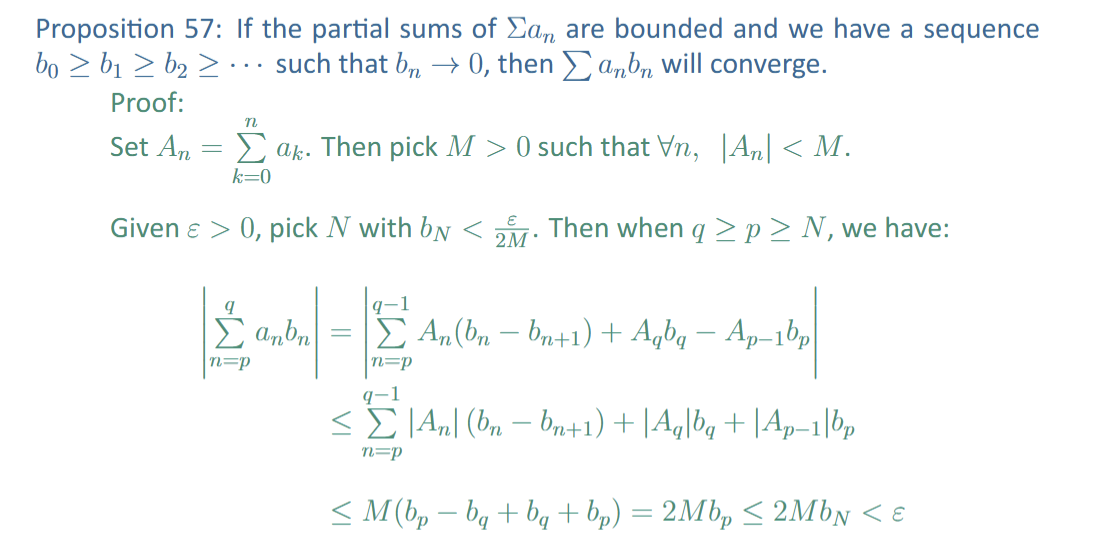
\includegraphics[scale=1]{Proof_HW3_math220a.png}\newpage\par}
	\end{itemize}
\end{myIndent}

\Hstatement\blab{Exercise III.2.1:} Show that $f(z) = |z|^2$ is complex differentiable only at the origin.

\begin{myIndent}\HexOne
	Identify $\mathbb{C}$ with $\mathbb{R}$ and consider $f$ as the function $f(x, y) = (x^2 + y^2, 0)$ going from $\mathbb{R}^2$ to $\mathbb{R}^2$. Then $f \in C^\infty(\mathbb{R}^2)$ with a derivative matrix $\left(\begin{smallmatrix}
	2x & 2y \\ 0 & 0
	\end{smallmatrix}\right)$. Now for $f$ to satisfy the Cauchy-Riemann equations (see the theorem on \inLinkRap{Cauchy-Riemann equations theorem}{page 296}) at a point $(x, y)$, we must have that $2x = 0$ and $-2y = 0$. Hence the only point where $f$ is complex differentiable is at\\ $(0, 0) = 0 + i0$.\retTwo
\end{myIndent}

\Hstatement\blab{Exercise III.2.3:} Show that $\lim_{n \to \infty} n^{1/n} = 1$.
\begin{myIndent}\HexOne
	If you want to prove this theorem without using logarithms (because you hadn't defined logarithms yet when you first relied on this fact), then here is the proof from math 140a:

	{\centering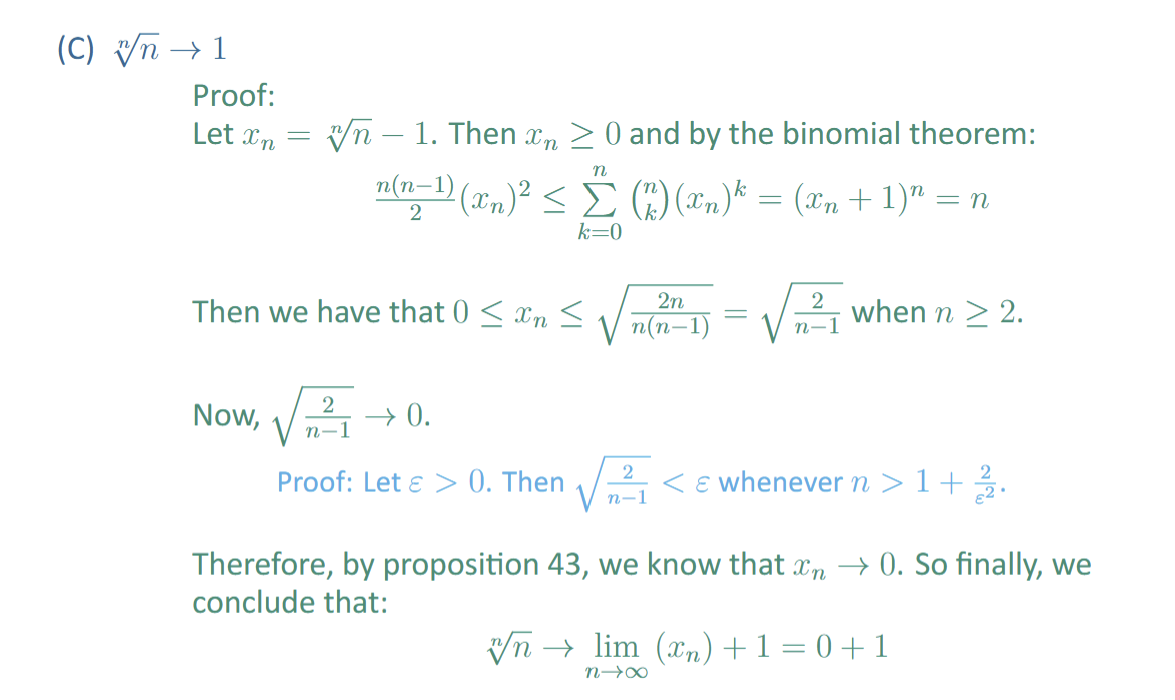
\includegraphics[scale=1]{Proof2_HW3_math220a.png}\retTwo\par}

	If you are willing to rely on logarithms and calculus though, then here is a slicker proof:
	\begin{myIndent}\HexTwoP
		Note that $\log(n^{1/n}) = \frac{1}{n}\log(n)$ for all $n$. Then by L'Hôpital's rule we have that $\lim_{x \to \infty}x^{-1}\log(x) = \lim_{x \to \infty}(1)^{-1}\frac{1}{x} = 0$. And hence $\log(n^{1/n}) \to 0$ as $n \to \infty$.\retTwo

		Finally, since $\exp$ is continuous, we have that $n^{1/n} = \exp(\log(n^{1/n})) \to \exp(0) = 1$ as $n \to \infty$.\retTwo
	\end{myIndent}
\end{myIndent}

\blab{Exercise III.2.19:} Let $G$ be a region and define $G^* = \{z : \overline{z} \in G\}$. If $f: G \to \mathbb{C}$ is holomorphic prove that $f^* : G^* \to \mathbb{C}$ defined by $f^*(z) = \overline{f(\overline{z})}$ is also holomorphic.

\begin{myIndent}\HexOne
	Once again identify $\mathbb{C}$ with $\mathbb{R}^2$ and write $f$ as $f(x, y) = (u(x, y), v(x, y))$. Then we have that $f^*(x, y) = (u(x, -y), -v(x, -y))$. And since $f$ is $C^1$, we can calculate that the derivative matrix of $f^*$ is $\Df (f^*) = \left(\begin{smallmatrix}
	u_x(x, -y) & -u_y(x, -y) \\ -v_x(x, -y) & v_y(x, y)
	\end{smallmatrix}\right)$.\retTwo

	Firstly, this shows that $f^*$ is also $C^1$ since all the partial derivatives of $f^*$ are continuous. Also, this shows that if $f$ satisfies the Cauchy-Riemann ewquations, then so does $f^*$. Hence $f$ being holomorphic on $G$ implies $f^*$ is as well.\retTwo
\end{myIndent}

\mySepTwo\newpage

\hTwo\dispDate{10/17/2025}

So for functional analysis I need some fixed point theorems that would normally have been taught in a topology class. But I've never taken an actual topology class. Hence, my goal for today is to prove those theorems. First, I will be taking notes from the paper \textit{Brouwer's Fixed Point Theorem} by Jasmine Katz. (See the \inLinkRap{bib citation 17}{17th entry} of the bibliography\dots)\retTwo

Katz defines a \udefine{convex body} in $\mathbb{R}^n$ to be a set $X \subseteq \mathbb{R}^n$ that is compact, convex, and has a nonempty interior (relative to the Euclidean topology of all of $\mathbb{R}^n$).\retTwo

Also, for $m \geq n \geq 1$ suppose we are given any $n + 1$ points $p_0, p_1 \ldots, p_n \in \mathbb{R}^m$ in general linear position (see my math 190b notes). Then we say the convex hull of those points (i.e. $\conv(p_0, p_1 \ldots, p_n)$) is an \udefine{$n$-simplex}. Recall from the notes I took before I dropped math 190b last Spring that all $n$-simplices are compact and homeomorphic to each other.\retTwo

Katz in particular denotes $\Delta_0^n \coloneqq \conv(e_1, \ldots, e_n, -\sum_{i=1}^n e_i)$ where $e_1, \ldots, e_n$ are\\ the standard basis vectors of $\mathbb{R}^n$. Also, Katz denotes $\Delta^n$ to be the \udefine{standard $n$-simplex}\\ $\conv(u_1, \ldots, u_{n+1})$ where $u_1, \ldots, u_{n+1}$ are the standard basis vectors of $\mathbb{R}^{n+1}$.\retTwo

\exTwo\ul{Proposition 3.2:} $\Delta_0^n$ is a convex body in $\mathbb{R}^n$.
\begin{myIndent}\exThreeP
	Proof:\\
	The only thing not trivial from the definition of $\Delta_0^n$ is that $\Delta_0^n$ has a nonempty interior. So to prove this, first define for each $k \in \mathbb{N}$ the $(k+1)$ by $(k+1)$ matrices:

	{\centering $A_k \coloneqq \begin{pmatrix}
		\begin{bmatrix} 1 & & \\ & \ddots & \\ & & 1 \end{bmatrix} & \begin{matrix} -1 \\ \vdots \\ -1 \end{matrix} \\ \begin{matrix} 1 & \cdots & 1 \end{matrix} & 1
	\end{pmatrix}$ and $B_k \coloneqq \begin{pmatrix}
		\begin{matrix} 0 \\ \vdots \\ 0 \end{matrix} & \begin{bmatrix} 1 & & \\ & \ddots & \\ & & 1 \end{bmatrix} \\ 1 & \begin{matrix} 1 & \cdots & 1 \end{matrix}
	\end{pmatrix}$ \retTwo\par}

	We can calculate the determinant of $A_k$ as follows:
	\begin{myIndent}\exPPP
		Clearly $\det(A_1) = \det(\left[ \begin{smallmatrix} 1 & -1 \\ 1 & 1 \end{smallmatrix}\right]) = 2$ and $\det(B_1) = \det(\left[ \begin{smallmatrix} 0 & 1 \\ 1 & 1 \end{smallmatrix}\right]) = -1$.\retTwo
		
		Meanwhile, by considering the Laplace expansions going along the top rows of $A_k$ and $B_k$ where $k > 1$, we get that:
		
		{\centering$\det(A_k) = \det(A_{k-1}) + (-1)^{k+3}\det(B_{k-1})$ and $\det(B_k) = -\det(B_{k-1})$\retTwo\par}

		From there it is easy to see that $\det(B_k) = (-1)^{k}$. And hence:
		
		{\centering\begin{tabular}{l}
			$\det(A_k) = \det(A_{k-1}) + (-1)^{(k + 3) + (k - 1)} = \det(A_{k-1}) + (-1)^{2(k + 1)}$\\
			$\phantom{\det(A_k) = \det(A_{k-1}) + (-1)^{(k + 3) + (k - 1)}} = \det(A_{k-1}) + 1$\\
			$\phantom{\det(A_k) = \det(A_{k-1}) + (-1)^{(k + 3) + (k - 1)}} = \det(A_{k-2}) + 2$\\
			$\phantom{\det(A_k) = \det(A_{k-1}) + (-1)^{(k + 3) + (k - 1)} = aaaaaaa} \vdots$\\
			$\phantom{\det(A_k) = \det(A_{k-1}) + (-1)^{(k + 3) + (k - 1)}} = \det(A_1) + (k-1) = k+1$\\
		\end{tabular}\retTwo\par}
	\end{myIndent}
	
	In particular, we now know that $A_n$ is invertible since it has nonzero determinant. And this is important because we can now say that $x = (x_1, \ldots, x_n) \in \Delta_0^n$ if and only if:
	
	{\centering\begin{tabular}{l}
		$f(x_1, \ldots, x_n) \coloneqq (A_n)^{-1}\left[\begin{smallmatrix} x_1 \\ \vdots \\ x_n \\ 1 \end{smallmatrix}\right] \in [0, \infty)^{n+1}$
	\end{tabular}\newpage\par}

	But $f$ is a continuous injection and $f(0) = (\frac{1}{n+1}, \ldots, \frac{1}{n+1})$ since:
	
	{\centering$0 = \sum_{i=1}^n \frac{1}{n + 1}e_i - \frac{1}{n+1}(\sum_{i=1}^n e_i)$.\retTwo\par}

	Hence, there must be some $\delta > 0$ such that $\|f(x) - f(0)\|_2 < \frac{1}{n+1}$ when $\|x\|_2 < \delta$. And in turn, the open ball of radius $\delta$ about $0$ is contained in $\Delta_0^n$. $\blacksquare$\retTwo
\end{myIndent}

\hTwo Katz defines a \udefine{ray} from $x_0 \in \mathbb{R}^n$ to be a set $\{x_0 + ty : t \geq 0\}$ where $y \in \mathbb{R}^n$ with $\|y\|_2 = 1$.\retTwo

\pracOne\mySepTwo
Here is a basic topology fact I somehow haven't proved before:\retTwo

\ul{Proposition:} Suppose $X$ is a topological space, $E \subseteq X$ is connected, and $A \subseteq X$ satisfies that $E \cap A \neq \emptyset$ and $E \cap A^\comp \neq \emptyset$. Then $E \cap \partial A \neq \emptyset$.
\begin{myIndent}\pracTwo
	Proof:\\
	Note that $\partial A = \overline{A} \cap \overline{A^\comp}$. So if $E \cap \partial A = \emptyset$, then this implies that $\overline{A} \cap E$ and $\overline{A^\comp} \cap E$\\ are two disjoint nonempty closed sets (in the subspace topology of $E$) whose union is\\ all of $E$. But this contradicts that $E$ is connected. $\blacksquare$
\end{myIndent}
\mySepTwo

\exTwo\ul{Lemma 3.6:} Suppose $X \subseteq \mathbb{R}^n$ is a convex body with $0 \in X^\circ$. Then every ray from $0$\\ intersects $\partial X$ exactly once.

\begin{myIndent}\exThreeP
	Proof:\\
	Fix $y \in \mathbb{R}^n$ such that $\|y\| = 1$ and let $f(t) = ty$. Then we want to show there is a unique $t_0 \geq 0$ such that $f(t_0) \in \partial X$. Fortunately, it's easy to see that $f(t)$ intercepts $\partial X$ at least once. After all, $f(0) \in X$. But at the same time, since $X$ is compact and thus bounded, we know that there is some $t^\prime > 0$ such that $f(t^\prime) \in X^\comp$. Since the ray traced by $f$ is connected, it now follows that there exists some $t_0 > 0$ such that $f(t_0) \in \partial X$.\retTwo

	We now show that our $t_0$ is unique. Suppose for the sake of contradiction that there exists $\varepsilon > 0$ with $(t_0 + \varepsilon)y \in X$. Then pick $r > 0$ such that the ball $\overline{B_r(0)} \subseteq X$. Since $X$ is convex, we know that any line segment from $(t_0 + \varepsilon)y$ to a point in $\overline{B_r(0)}$ is contained\\ [2pt] in $X$. And thus, while it is fucking awful to calculate, we have that the open ball of radius\\ [2pt] $R = \min(t_0, \sqrt{Q(t_{\min})})$ about $t_0 y$ is contained in $X$ where:\\ [-20pt] 
	
	{\centering$Q(t) = (r - \frac{r}{t_0 + \varepsilon}t)^2 + (t - t_0)^2$ and $t_{\min} = \frac{\frac{r^2}{t_0 + \varepsilon} + t_0}{\frac{r^2}{(t_0 + \varepsilon)^2} + 1}$ \retTwo\par}

	\begin{tabular}{p{2in} p{4in}}
	For a hint at how I got that\newline fucked up radius $R$, observe\newline the diagram to the right:\retTwo
	
	However, the fact we were\newline able to find such an $R$\newline contradicts that $t_0 y \in \partial X$.\newline Hence, our supposed $\varepsilon$ can't\newline exist.&

	{\center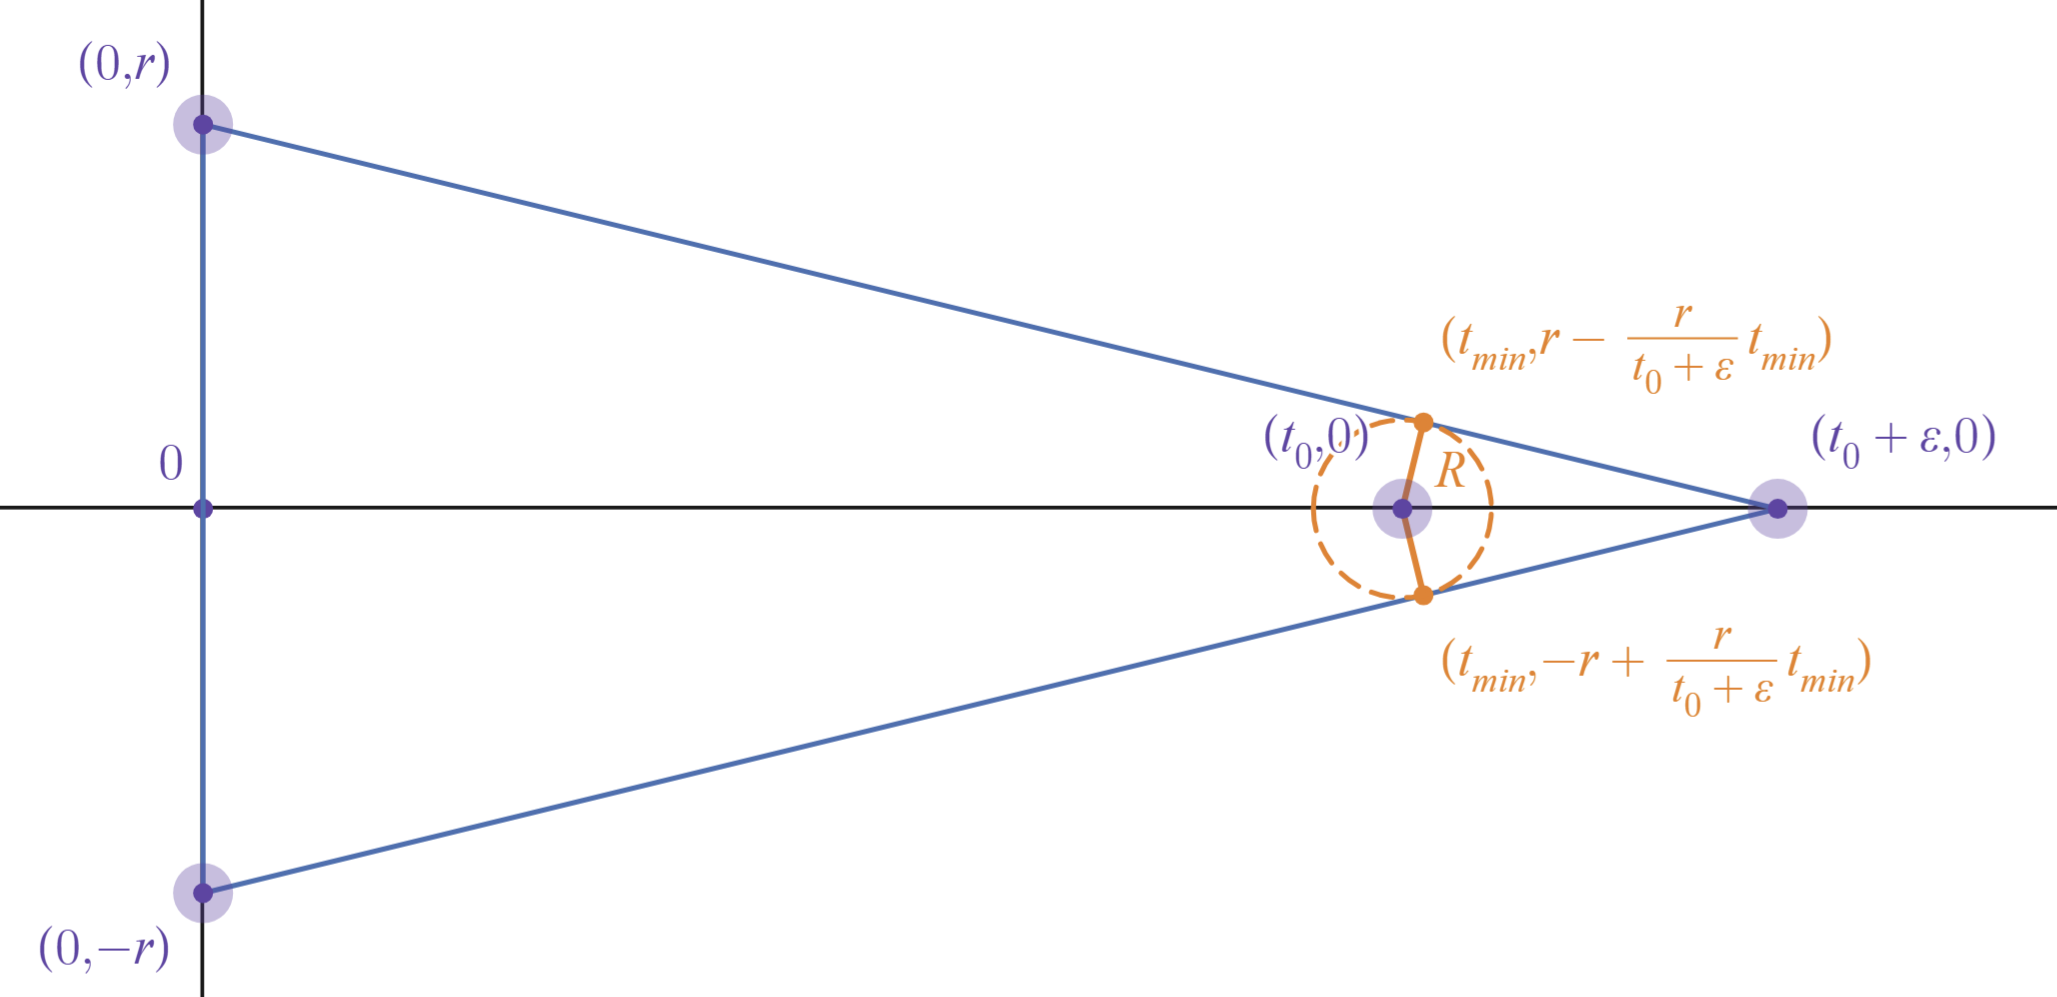
\includegraphics[scale=0.44]{Doing_Geometry_page_318.png}\par}
	\end{tabular}

	\newpage

	Since $X$ is closed (since it's compact) and thus includes it's boundary, we've now proven that if $f(t_0) \in \partial X$ then $f(t) \notin \partial X$ for all $t > t_0$. And hence, our ray can intercept $\partial X$ at most once. $\blacksquare$
	\begin{myIndent}\myComment
		As a side note: something even more fucked up is that the radius proposed by this paper doesn't work. It's too large. Anyways, because the paper handwaves this next bit, I'm going to deviate from the paper a bit.\retTwo
	\end{myIndent}
\end{myIndent}

\pracOne\mySepTwo
\ul{Lemma:} \hypertarget{page 318 lemma}{Let} $\mathcalli{X}$ be a topological $K$-vector space where $K = \mathbb{R}$ or $\mathbb{C}$. Also suppose $E \subseteq X$ and $c \in K$. 
\begin{itemize}
	\item If $E$ is convex, then so is $cE$.
	\begin{myIndent}\pracTwo
		Proof:\\
		If $E$ is empty or $c = 0$, this is obvious. Otherwise, suppose $x, y \in cE$ and then note that $c^{-1}x, c^{-1}y \in E$. It follows that $c^{-1}(tx + (t-1)y) \in E$. So, $tx + (1-t)y \in cE$.\retTwo
	\end{myIndent}

	\item $c(\overline{E}) = \overline{cE}$.
	\begin{myIndent}\pracTwo
		Proof:\\
		If $c = 0$ then it must be the case that both sets are empty or are $\{0\}$. Meanwhile, note that as a general fact if $f : X \to Y$ is a continuous map and $A \subseteq X$, then $f^{-1}(\overline{f(A)})$ is a closed set containing $A$. Hence $\overline{A} \subseteq f^{-1}(\overline{f(A)})$ and this proves that $f(\overline{A}) \subseteq \overline{f(A)}$. Since scalar multiplication by $c$ is a homeomorphism of $\mathcalli{X}$ when $c \neq 0$, we thus have that $c\overline{E} = \overline{cE}$. $\blacksquare$\retTwo
	\end{myIndent}

	\item $c(\partial E) = \partial (cE)$.
	\begin{myIndent}\pracTwo
		Proof:\\
		By the last bullet point plus the fact that $f(A \cap B) = f(A) \cap f(B)$ for any function, we know that $c(\partial E) = c(\overline{E} \cap \overline{E^\comp}) = \overline{cE} \cap \overline{c(E^\comp)}$. Now if $c = 0$, then we know that $c(\partial E)$ and $\partial (cE)$ are either both empty or both $\{0\}$. So, we may assume that $c \neq 0$. But in that case scalar multiplication is a homeomorphism on $\mathcalli{X}$. So $c(E^\comp) = (cE)^\comp$ and we've shown that $c(\partial E) = \overline{cE} \cap \overline{(cE)^\comp} = \partial (cE)$.\retTwo
	\end{myIndent}
\end{itemize}

\ul{Lemma:} Suppose $f: X \to Y$ is a homeomorphism and $A, B \subseteq X$. (This would include the case that $X = Y = \mathcalli{X}$ and $f$ is scalar multiplication by a nonzero scalar). Then\\ $f(E^\circ) = (f(E))^\circ$.
\begin{myIndent}\pracTwo
	Proof:\\
	Since $f$ is continuous and bijective, $f^{-1}(f(A)^\circ)$ is an open set contained in $A$. So,\\ $f^{-1}(f(A)^\circ) \subseteq A^\circ$ and hence $f(A)^\circ \subseteq f(A^\circ)$. On the other hand, since $f^{-1}$ is\\ continuous, we know that $f(A^\circ)$ is an open subset of $f(A)$. So, $f(A^\circ) \subseteq f(A)^\circ$.\retTwo
\end{myIndent}

\mySepTwo

\exTwo\ul{Theorem:} Suppose $X \subseteq \mathbb{R}^n$ is a convex body and contains $0$. Then $X$ is homeomorphic to the closed unit ball $\overline{B_1(0)}$.

\begin{myIndent}\exThreeP
	Proof:\newpage
	Let $p_{X^\circ}$ be the Minkowski functional associated with $X^\circ$. In other words,\\ $p_{X^\circ}(x) = \inf \{t \geq 0 : x \in tX\}$. Unfortunately, since $X$ isn't a balanced set\\ necessarily, we can't directly apply the proof on \inLinkRap{Minkowski functional reference}{page 233} to get that $P_{X^\circ}(cx) = |c|x$\\ for all $c \in \mathbb{R}$ and $x \in \mathbb{R}^n$. That said, since $X$ is convex and a neighborhood of $0$, we are able to copy the reasoning that shows that $p_{X^\circ}$ is well-defined and satisfies the triangle inequality.\retTwo

	\ul{Claim 1:} Suppose $y$ is any unit vector and $t_0$ is the unique nonnegative number satisfying that $t_0 y \in \partial X$. Then $p_{X^\circ}(ty) = \sfrac{t}{t_0}$.
	\begin{myIndent}\exPPP
		Proof:\\
		If $t = 0$, then it is obvious that $p_{X^\circ}(ty) = 0 = \sfrac{t}{t_0}$. As for when $t \neq 0$, first note that $t_0 y \in \partial X \Longleftrightarrow bt_0 y \in \partial(bX)$ for all $b \geq 0$. Also note that $bX$ is easily checked to be convex body when $b \neq 0$ (and so we can apply theorem 3.6 to $bX$).\retTwo

		Suppose $b < \sfrac{t}{t_0}$. Then $bt_0 < t$ and thus $t \notin X$ since $bt_0 y \in \partial (bX)$. On the other hand, suppose $b > \sfrac{t}{t_0}$. Then $bt_0 > t$ and thus $t \in X - \partial X = X^\circ$ since again $bt_0 y \in \partial (bX)$. It follows that $p_{X^\circ}(ty) = \sfrac{t}{t_0}$.\retTwo
	\end{myIndent}

	\ul{Corollary:} Suppose $x \in X$ and $t_0 > 0$ is the unique nonnegative number such that\\ $t_0 \frac{x}{\|x\|_2} \in \partial X$. Then $p_{X^\circ}(x) = \sfrac{\|x\|_2}{t_0}$.\retTwo

	\ul{Claim 2:} $p_{X^\circ}$ is continuous.
	\begin{myIndent}\exPPP
		Proof:\\
		While we don't necessarily have reverse triangle inequality since $p_{X^\circ}(x) \neq p_{X^\circ}(-x)$, we can at least prove using just triangle inequality that:

		{\centering $|p_{X^\circ}(x) - p_{X^\circ}(y)| \leq \max(p_{X^\circ}(x - y), p_{X^\circ}(y - x))$ \retTwo\par}

		Then, you just need to follow almost identical reasoning to that of \inLinkRap{Minkowski functional reference}{page 233} to show that $p_{X^\circ}(x)$ is continuous.\retTwo
	\end{myIndent}

	At last we are ready to write our homeomorphism from $X$ to $B$. Define $g : X \to \overline{B_1(0)}$ by $g(x) = p_{X^\circ}(x)\frac{x}{\|x\|_2}$ when $x \neq 0$ and $g(0) = 0$. And similarly, define $h : \overline{B_1(0)} \to X$ by $h(y) = ty$ such that $ty \in \partial(\|y\|X)$.
	\begin{itemize}
		\item $g$ is continuous when $x \neq 0$ by virtue of being a scalar product of continuous\\ functions. Also, given any sequence $(x_n)_{n \in \mathbb{N}}$ in $X$ converging to $0$ we have that\\ $\|g(x_n)\|_2 = p_{X^\circ}(x_n) \cdot 1 \to 0$ as $n \to \infty$. So $g$ is also continuous at $0$.\retTwo
		
		\item $h(g(0)) = 0$. Meanwhile, suppose $x \in X - \{0\}$. Then let $t_0$ be the unique\\ [2pt] nonnegative number satisfying that $t_0 \frac{x}{\|x\|_2} \in \partial X$. Now $g(x) = p_{X^\circ}(x) \frac{x}{\|x\|_2} = \frac{x}{t_0}$.\\ [-1pt] Thus $h(g(x)) = t \frac{x}{t_0}$ where $t \geq 0$ satisfies that $t \frac{x}{t_0} \in \partial(\frac{\|x\|}{t_0}X)$. Or in other words,\\ [3pt] $t\frac{x}{\|x\|_2} \in \partial X$. It follows by theorem 3.6 that $t = t_0$ and so $h(g(x)) = x$.\retTwo
		
		\item $g(h(0)) = g(0) = 0$. Meanwhile, if $y \in \overline{B_1(0)} - \{0\}$ then let $t_0$ be the\\ unique nonnegative number such that $t_0 \frac{y}{\|y\|_2} \in \partial X$. Like before, we can show\\ that $h(y) = t_0 y$. And now $p_{X^\circ}(t_0 y) = \frac{t_0\|y\|_2}{t_0} = \|y\|_2$ since $t_0 y = t_0 \|y\|_2 \frac{y}{\|y\|_2}$.\\ Thus $g(t_0 y) = g(t_0 y) = \|y\|_2\frac{t_0y}{\|t_0y\|_2} = y$ and we've proven that $g(h(y)) = y$.\newpage
		
		\item Since $h = g^{-1}$, $g$ is continuous, $X$ is compact, and $\overline{B_1(0)}$ is Hausdorff, we have that $h$ is continuous. $\blacksquare$\retTwo
	\end{itemize}
\end{myIndent}

\ul{Corollary:} All convex bodies in $\mathbb{R}^n$ are homeomorphic to the closed unit ball $\overline{B_1(0)}$.
\begin{myIndent}\exThreeP
	Why? We can just translate them so that they contain $0$ and then apply the last theorem.\retTwo
\end{myIndent}

\ul{Corollary 2:} All $n$-simplices are homeomorphic to the closed unit ball $\overline{B_1(0)}$ in $\mathbb{R}^n$.\retTwo

\hTwo\mySepTwo 

\dispDate{10/18/2025}

I need to first do the rest of my math 200a homework. Then I think there is a different paper I want to try to following to prove the fixed point theorems from before.\retTwo

\blect{Math 200a Homework:}\retTwo

\Hstatement\blab{Set 3 Problem 3:} Suppose $G$ is a finite group and $h < G$. Suppose also for all $x \in H - \{1\}$ that $C_G(x) \subseteq H$. Then $\gcd(|H|, [G : H]) = 1$.
\begin{myIndent}\HexOne
	Proof:\\
	If $\gcd(|H|, [G : H]) \neq 1$, then we know there is some prime number $p$ dividing both $|H|$ and $[G : H]$. And as a result, $\nu_p(|H|) < \nu_p(|G|)$. So, by choosing $P \in \Syl_p(H)$ and $Q \in \Syl_p(G)$, we know that $|P| < |Q|$. Also, by Sylow's second theorem, we can conjugate $Q$ in order to say without loss of generality that $P \subseteq Q$. We'll need two observations:
	\begin{itemize}
		\item Since the order of $Q$ doesn't divide $H$, we know that $Q$ isn't a subgroup of $H$. Hence, $Q \cap (G - H) \neq \emptyset$.
		\item At the same time though, we know that $P < Q \cap H < H$. And since the only prime factors of $|Q \cap H|$ are $p$, this tells us by Lagrange's theorem that $|P| = p^{\nu_p(|H|)}$ divides $|Q \cap H|$ which itself divides $p^{\nu_p(|H|)}$. Hence, $|P| = |Q \cap H|$ and this proves that $Q \cap H = P$. \retTwo
	\end{itemize}

	Now recall from the 2nd proposition on \inLinkRap{Alireza theorem center of p groups}{page 272} that if $\{1\} \neq N \lhd P$ and $P$ is a $p$-group, then $Z(P) \cap N \neq \{1\}$.
	\begin{myIndent}\exPPP
		Side note: Whenever $H < G$, we define $Z(H) = \bigcap_{h \in H}C_H(h)$. Just wanted to make that's clear since I didn't know better before.\retTwo
	\end{myIndent}

	As a special case, if we set $N = P$ (where $P$ is nontrivial), then this proposition says that the center of a $p$-group is always nontrivial. Hence, there exists $y \in Z(P) - \{1\}$.
	\begin{myIndent}\exPPP
		Side note: How the hell hadn't I processed that consequence of the theorem we\\ proved before?\retTwo
	\end{myIndent}

	Now note that $Z(Q) \subseteq C_Q(y) \subseteq C_G(y) \subseteq H$ where the last inclusion is by the\\ assumption of the problem. Hence $Z(Q) \subseteq H \cap Q = P$. At the same time, we know\\ that $Z(Q)$ is nontrivial. So, there exists $x \in Z(Q) - \{1\}$ which we know from before is\\ in $P \subseteq H$. Finally, we now have that $Q \subseteq C_Q(x) \subseteq C_G(x) \subseteq H$. But this contradicts that $Q \cap (G - H) \neq \emptyset$. $\blacksquare$\retTwo
\end{myIndent}

\blab{Set 3 Problem 8:} Suppose $G$ is a finite group.
\begin{enumerate}
	\item[(a)] Prove that a normal Sylow $p$-subgroup is a characteristic subgroup.\newpage
	
	\begin{myIndent}\HexOne
		A Sylow $p$-subgroup $P$ is normal if and only if it is the only Sylow $p$-subgroup. And since automorphisms preserve the order of subgroups, we have that if $P$ is the only subgroup of $G$ with order $p^{\nu_p(|G|)}$ then $\theta(P) = P$ for all $\theta \in \Aut(G)$. So, $P$ is a characteristic subgroup.\retTwo
	\end{myIndent}
	
	\item[(b)] Suppose $H \lhd G$ and $\gcd(|H|, [G : H]) = 1$. Prove that $H$ is a characteristic subgroup.
	
	\begin{myIndent}\HexOne
		Suppose $\theta \in \Aut(G)$. Then since $H$ is normal, we know that $\theta(H)H$ is a subgroup of $G$ and $H \lhd \theta(H)H$. So by the correspondance theorem, we know that $|\frac{\theta(H)H}{H}|$ divides $|G/H| = [G : H]$. At the same time, $|\theta(H)H| = \frac{|H||\theta(H)|}{|H \cap \theta(H)}$. So, $|\frac{\theta(H)H}{H}| = \frac{|\theta(H)|}{|H \cap \theta(H)}$ divides $|\theta(H)| = |H|$.\retTwo

		This shows that $|\frac{\theta(H)H}{H}| \divides \gcd(|H|, [G : H]) = 1$. And hence, $\theta(H)H = H$. Since $|\theta(H)| = |H|$ and $\theta(H) \subseteq \theta(H)H$, we can thus conclude that $\theta(H) = H$. $\blacksquare$\retTwo
	\end{myIndent}
\end{enumerate}

\blab{Set 3 Problem 4:} Suppose $G$ is a finite group, $N \lhd G$, and $p$ is a prime factor of $|N|$.
\begin{myIndent}
	\item[(a)] Suppose $P \in \Syl_p(G)$ and $Q \in \Syl_p(N)$. Prove there exists $g \in G$ such that\\ $Q = (gPg^{-1}) \cap N$.
	
	\begin{myIndent}\HexOne
		Uhhhh, I think I already basically proved this fact when doing problem 3.\retTwo

		By Sylow's second theorem, we know there is some $g \in G$ such that $Q \subseteq gPg^{-1}$. Then since $(gPg^{-1}) \cap N$ is a subgroup of $gPg^{-1}$ where the latter is a $p$-group, we know that $(gPg^{-1}) \cap N$ is also a $p$-group. Also, since $(gPg^{-1}) \cap N$ is a subgroup of $N$, we know that $|(gPg^{-1}) \cap N|$ divides $|N|$. It follows that $|(gPg^{-1}) \cap N|$ divides $p^{\nu_p(|N|)}$. At the same time, since $|Q| = p^{\nu_p(|N|)}$ and $Q \subseteq gPg^{-1} \cap N$, we have that $p^{\nu_p(|N|)} \leq |(gPg^{-1}) \cap N|$.\retTwo

		So, $Q \subseteq (gPg^{-1}) \cap N$ and $|Q| = p^{\nu_p(|N|)} = |(gPg^{-1}) \cap N|$. It follows that\\ $Q = (gPg^{-1}) \cap N$.
		\begin{myIndent}\myComment
			Side note: none of the reasoning in this part requires having $N$ be normal.\retTwo
		\end{myIndent}
	\end{myIndent}
	
	\item[(b)] Prove that the following is a well-defined surjective function:
	
	{\centering $\Phi : \Syl_p(G) \to \Syl_p(N)$ where $\Phi(P) = P \cap N$. \retTwo\par}

	\begin{myIndent}\HexOne
		Part (a) guarentees that the above map will be surjective provided that it is well-\\defined (since $gPg^{-1} \in \Syl_p(G)$ for any $P \in \Syl_p(G)$). Hence, all we need to show\\ is that $P \cap N \in \Syl_p(N)$ whenever $P \in \Syl_p(G)$.\retTwo

		Fortunately since $P \cap N < P$, we know that $P \cap N$ is a $p$-group. But suppose for\\ the sake contradiction that $|P \cap N| \neq p^{\nu_p(|N|)}$ (meaning $P \cap N \notin \Syl_p(G)$). Then,\\ by Sylow's first and second theorems there exists a group $Q \in \Syl_p(N)$ such that\\ $P \cap N \lneqq Q < N$. Also, by part (a) there exists $g \in G$ such that $Q = gPg^{-1} \cap N$. But since $N$ is normal, $gPg^{-1} \cap N = gPg^{-1} \cap gNg^{-1} = g(P \cap N)g^{-1}$.
		\begin{myIndent}\HexPPP
			The last equality is obvious if you think about it. So I'd rather not write out a proof since I want to go on an outing soon.\retTwo
		\end{myIndent}

		So $P \cap N \lneqq Q = g(P \cap N)g^{-1}$. Since $|P \cap N| = |g(P \cap N)g^{-1}|$ this is a contradiction.\newpage
	\end{myIndent}

	\item[(c)] For $P \in \Syl_p(G)$, prove that $N_G(P) \subseteq N_G(\Phi(P))$ and:
	
	{\centering $|\Phi^{-1}(\Phi(P))| = [N_G(\Phi(P)) : N_G(P)]$. \retTwo\par}

	\begin{myIndent}\HexOne
		To start off, note that:
		
		{\centering\begin{tabular}{l}
			$\Phi(xPx^{-1}) = xPx^{-1} \cap N = xPx^{-1} \cap xNx^{-1}$\\
			$\phantom{\Phi(xPx^{-1}) = xPx^{-1} \cap N} = x(P \cap N)x^{-1} = x\Phi(P)x^{-1}$.
		\end{tabular}\retTwo\par}

		Therefore, if $x \in N_G(P)$ then $\Phi(P) = \Phi(xPx^{-1}) = x\Phi(P)x^{-1}$. And this proves the first claim that $N_G(P) \subseteq N_G(\Phi(P))$.\retTwo

		Next, note by Sylow's second theorem that:
		
		{\centering$\Phi^{-1}(\Phi(P)) = \{gPg^{-1} : g \in G \text{ and } \Phi(P) \subseteq gPg^{-1}\}$.\retTwo\par}

		But $\Phi(P) \subseteq gPg^{-1}$ if and only if:
		
		{\centering\begin{tabular}{l}
			$\Phi(P) = P \cap N \subseteq gPg^{-1} \cap N = (gPg^{-1}) \cap (gNg^{-1})$\\
			$\phantom{\Phi(P) = P \cap N \subseteq gPg^{-1} \cap N} = g(P \cap N)g^{-1} = g\Phi(P)g^{-1}$.
		\end{tabular}\retTwo\par}

		And since $|\Phi(P)| = |g\Phi(P)g^{-1}|$, this is the same as saying that $\Phi(P) = g\Phi(P)g^{-1}$. So, we really have that:

		{\centering$\Phi^{-1}(\Phi(P)) = \{gPg^{-1} : g \in N_G(\Phi(G))\}$.\retTwo\par}

		Hence, if we consider the action $N_G(\Phi(P)) \curvearrowright \Syl_p(G)$ by conjugation, then\\ [-1pt] $\Phi^{-1}(\Phi(P))$ is precisely the orbit of $P$ with respect to this action. Also, $x$ is in the stabilizer of $P$ with respect to this action precisely when $xPx^{-1} = P$. Or in other\\ words, $x \in (N_G(\Phi(P)))_P$ when $x \in N_G(\Phi(P)) \cap N_G(P) = N_G(P)$. By the\\ orbit-stabilizer theorem, we thus can conclude that:
		
		{\centering$|\Phi^{-1}(\Phi(P))| = [N_G(\Phi(P)) : N_G(P)]$.\retTwo\par}
	\end{myIndent}

	\item[(d)] Prove that $|\Syl_p(N)|$ divides $|\Syl_p(G)|$.
	
	\begin{myIndent}\HexOne
		We know that $\{\Phi^{-1}(Q) : Q \in \Syl_p(N)\}$ forms a partion of $\Syl_p(G)$. Hence, we\\ [-2pt] now seek to prove that there exists a single integer $r \in \mathbb{N}$ such that $|\Phi^{-1}(Q)| = r$ for all $Q \in \Syl_p(N)$. After all, once we know that we will then be able to say that $\Syl_p(N) = r \Syl_p(G)$.\retTwo

		Luckily, note that since conjugation is an automorphism of $G$ we have that:
		\begin{itemize}
			\item $|N_G(P)| = |g(N_G(P))g^{-1}| = |(N_G(gPg^{-1}))|$,
			\item $|N_G(\Phi(P))| = |g(N_G(\Phi(P)))g^{-1}| = |N_G(g\Phi(P)g^{-1})| = |N_G(\Phi(gPg^{-1}))|$.\retTwo
		\end{itemize}

		It follows for all $g \in G$ and $P \in \Syl_p(G)$ that:

		{\centering\begin{tabular}{l}
			$|\Phi^{-1}(\Phi(P))| = [N_G(\Phi(P)) : N_G(P)]$ \\ [4pt]
			$\phantom{|\Phi^{-1}(\Phi(P))|} = \frac{|N_G(\Phi(P))|}{|N_G(P)|} = \frac{|N_G(\Phi(gPg^{-1}))|}{|N_G(gPg^{-1})|} = [N_G(\Phi(gPg^{-1})) : N_G(gPg^{-1})]$\\
			$\phantom{|\Phi^{-1}(\Phi(P))| = \frac{|N_G(\Phi(P))|}{|N_G(P)|} = \frac{|N_G(\Phi(gPg^{-1}))|}{|N_G(gPg^{-1})|}} = |\Phi^{-1}(\Phi(gPg^{-1}))|$
		\end{tabular}\retTwo\par}

		And since $G$ acts transitively on $\Syl_p(G)$ by conjugation, this means that there exists\\ $r \in \mathbb{N}$ such that $r = |\Phi^{-1}(\Phi(P))|$ for all $P \in \Syl_p(G)$. And since $\Phi$ is surjective,\\ we have that $\Phi^{-1}(Q) = r$ for all $Q \in \Syl_p(G)$. $\blacksquare$\newpage
	\end{myIndent}
\end{myIndent}

\hTwo I'm now going to follow the paper: \textit{The Milnor-Rogers Proof of the Brouwer Fixed Point Theorem}, by Ralph Howard (see bibliography \inLinkRap{bib citation 18}{item 18}).\retTwo

For ease of notation, I will denote $B^{n} \coloneqq \{x \in \mathbb{R}^n : \|x\|_2 < 1\}$, and $S^{n-1} = \partial B^n$. Also, let $e_1, \ldots, e_n$ be the standard basis vectors for $\mathbb{R}^n$.\retTwo

\exTwo\ul{Lemma:} Suppose $f: \overline{B^n} \to \mathbb{R}^m$. As a reminder, this means there is an open set\\ [2pt] $\overline{B^n}\subseteq U \subseteq \mathbb{R}^n$ and a function $g : U \to \mathbb{R}^m$ such that $g|_{\overline{B^n}} = f$. We claim that\\ [0pt] if $x = (x_1, \ldots, x_n) \in S^{n-1}$, then $\frac{\partial}{\partial x_j}g(x)$ is entirely determined by $f$.

\begin{myIndent}\exThreeP
	Proof:\\
	To start off, note that $\|x + he_j\|_2^2 = \|x\|_2^2 + 2(x \cdot he_j) + h^2\|e_j\|_2^2 = 1 + 2hx_j + h^2$.\\ Thus $\|x + he_j\|_2 \leq 1$ when $h(2x_j + h) \leq 0$. And so either $h \in (-2x_j, 0]$ or\\ $h \in [0, -2x_j)$. It follows that:
	\begin{itemize}
		\item if $x_j > 0$, then $\frac{\partial}{\partial x_j} g(x) = \lim\limits_{h \to 0} \frac{g(x + he_j) - g(x)}{h} = \lim\limits_{h \to 0^{-}} \frac{f(x + he_j) - f(x)}{h}$;
		\item if $x_j < 0$, then $\frac{\partial}{\partial x_j} g(x) = \lim\limits_{h \to 0} \frac{g(x + he_j) - g(x)}{h} = \lim\limits_{h \to 0^{+}} \frac{f(x + he_j) - f(x)}{h}$.\retTwo
	\end{itemize}

	This shows that so long as $x_j = (x \cdot e_j) \neq 0$, we have that $\frac{\partial}{\partial x_j} g(x)$ is entirely determined\\ [-4pt] by $g$'s restriction to $\overline{B^n}$ (i.e. $f$).\retTwo.

	Meanwhile, suppose $x_j = 0$ and define $\alpha(t) = \cos(t)x + \sin(t)e_j$. Then $\alpha$ is smooth an\\ [2pt]  so $\nabla g(\alpha(t)) \cdot \alpha^\prime(t)$ will be a continuous function converging to $\frac{\partial}{\partial x_j} g(x)$ as $t \to 0$. But\\ also note that for any $i \neq j$ we have that  $\alpha^\prime(t) \cdot e_i = -\sin(t)x_i$. So for any $t \in \mathbb{R}$, we\\ [3pt] have that:

	{\center\begin{tabular}{l}
		$\nabla g(\alpha(t)) \cdot \alpha^\prime(t) = \cos(t)\frac{\partial}{\partial x_j}g(\alpha(t)) -  \hspace{-0.3em}\sum\limits_{\begin{smallmatrix}
		1 \leq i \leq n \\ i \neq j
		\end{smallmatrix}}\hspace{-0.3em} \sin(t)x_i\frac{\partial}{\partial x_i} g(\alpha(t)) $\\ [25pt]

		$\phantom{\nabla g(\alpha(t)) \cdot \alpha^\prime(t)}  = \cos(t)\frac{\partial}{\partial x_j}g(\alpha(t)) -  \hspace{-0.3em}\sum\limits_{\begin{smallmatrix}
		1 \leq i \leq n \\ x_i \neq 0
		\end{smallmatrix}}\hspace{-0.3em} \sin(t)x_i\frac{\partial}{\partial x_i} g(\alpha(t)) $\\ [12pt]
	\end{tabular}\retTwo\par}

	Next note that if $x_i \neq 0$ and $i \neq j$, then $\alpha(t) \cdot e_i = cos(t)x_i \neq 0$ for all $t \in (-\sfrac{\pi}{2}, \sfrac{\pi}{2})$. Thus, by our prior work we know for all $t \in (-\sfrac{\pi}{2}, \sfrac{\pi}{2})$ that $\frac{\partial}{\partial x_i}g(\alpha(t))$ is determined by\\ [-1pt] $f$ provided that $x_i \neq 0$. At the same time, for all $t \in (-\sfrac{\pi}{2}, \sfrac{\pi}{2}) - \{0\}$, we have that $\alpha(t) \cdot e_j = \sin(t) \neq 0$. Thus by our prior work, we know that $\frac{\partial}{\partial x_i}g(\alpha(t))$ is determined by $f$ for all $t \in (-\sfrac{\pi}{2}, \sfrac{\pi}{2}) - \{0\}$.\retTwo

	And now we are done as the limit of $\nabla g(\alpha(t)) \cdot \alpha^\prime(t)$ as $t \to 0$ is uniquely determined\\ by $f$. $\blacksquare$\retTwo
\end{myIndent}

\hTwo As a result, if $f \in C^r(\overline{B^n})$ (where $r \geq 1$) then we can without ambiguity refer to $f$ as having partial derivatives on $S^{n-1}$. Also, by an application of \inLinkRap{John Lee Proposition C.29}{proposition C.29} on page 291, we have that if $f \in C^1(\overline{B^n})$ then $f$ is Lipschitz.\retTwo

With that out of the way, I'm now ready to get into Howard's paper.\newpage

\exTwo\ul{Lemma 1:} There is no $C^1$ map $f : \overline{B^n}\to S^{n-1}$ such that $f(x) = x$ for all $x \in S^{n-1}$.

\begin{myIndent}\exThreeP
	Proof:\\
	Assume such an $f$ exists and for $t \in [0, 1]$ let $f_t(x) \coloneqq (1 - t)x + tf(x) = x + tg(x)$\\ (where $g(x) \coloneqq f(x) - x$). Then note that for all $x \in \overline{B^n}$:
	
	{\centering$\|f_t(x)\|_2 \leq (1-t)\|x\|_2 + t\|f(x)\|_2 \leq (1-t) + t = 1$.\retTwo\par}

	Hence, $f_t$ maps $\overline{B^n}$ into $\overline{B^n}$. Also, $f_t$ fixes $S^{n-1}$ as:
	
	{\centering$f_t(x) = (1-t)x + tf(x) = (1-t)x + tx = x$.\retTwo\par}

	Now $g$ is $C^1$ since $f$ is. So, let $C > 0$ be a Lipschitz constant for $g$ (i.e. for all $x_1, x_2 \in \overline{B^n}$\\ we have that $\|g(x_2) - g(x_1)\|_2 \leq C\|x_2 - x_1\|_2$). Using this fact, we claim that when $t$\\ is small enough then $f_t$ is injective. After all, suppose there eixsts distinct $x_1, x_2 \in \overline{B^n}$\\ with $f_t(x_1) = f_t(x_2)$. Then $x_2 - x_1 = t(g(x_1) - g(x_2))$. So:

	{\centering $\|x_2 - x_1\|_2 = t\|g(x_2) - g(x_1)\|_2 \leq tC\|x_2 - x_1\|_2$ \retTwo\par}

	And since $\|x_2 - x_1\|_2 > 0$, this means that $tC \geq 1$. So if $t < \sfrac{1}{C}$, then we must have that $f_t$ is injective.\retTwo

	Next, for each $t \in [0, 1]$ let $G_t \coloneqq f_t(B^n)$. We claim that if $t$ is small enough then  $G_t$ is open. To see why, let $L(\mathbb{R}^n)$ be the space of linear maps from $\mathbb{R}^n$ to itself equipped with the standard operator norm. Then $A(x, t) = (f_t)^\prime(x) = \myId + tg^\prime(x)$ is a well-defined map from $\overline{B^n} \times [0, 1]$ to $L(\mathbb{R}^n)$ that is continuous with respect to $t$ and with respect to $x$ (I'm not sure and don't really care to prove if it is continuous with respect to $x$ and $t$ jointly).\retTwo

	By the extreme value theorem, we know there exists $M = \max(\|g^\prime(x)\|_{\opnorm} : x \in \overline{B^n})$. And then since the set of invertible maps in $L(\mathbb{R}^n)$ is open, we know there is some $r > 0$ such that $A(x, t)$ is invertible when $\|A(x, t) - \myId\|_{\opnorm} = t\|g^\prime(x)\|_{\opnorm} \leq r$. Thus, when $t \leq \frac{r}{M}$, we know that $A(x, t) = (f_t)^\prime(x)$ is invertible for all $x$. And now it follows from the inverse function theorem (see my math 140c notes) that $f_t$ restricted to $B^n$ is an open map when $t \leq \frac{r}{M}$.\retTwo

	By letting $t_0 = \min(\sfrac{1}{C}, \sfrac{r}{M}) > 0$, we have thus shown that $f_t$ is injective and that $G_t$ is open for all $t \in [0, t_0]$. One more claim we'll make before we get to the main part of the proof is that $G_t = B^n$ when $t \in [0, t_0]$. To show this, note that since $f_t$ is injective, we know that $G_t \subseteq \overline{B^n} - S^{n-1} = B^n$.\retTwo

	Now for the sake of contradiction suppose $G_t \neq B^n$. Then we know that $(\partial G_t) \cap B^n \neq \emptyset$. In particular, let $y^{(0)} \in (\partial G_t) \cap B^n$ and then consider a sequence $\{x_\ell\}_{\ell \in \mathbb{N}}$ in $B^n$ such that $f_t(x_\ell) \to y_0$ as $\ell \to \infty$. By the compactness of $\overline{B^n}$, we can pass to a subsequence to say without loss of generality that $x_\ell \to x^{(0)}$ as $\ell \to \infty$ for some $x^{(0)} \in \overline{B^n}$.\retTwo
	
	By the continuity of $f$, we know that $f(x^{(0)}) = y^{(0)}$. But also note that since $G_t$ is open, we know $y^(0) \notin G_t$. Hence $x^{(0)} \in \overline{B^n} - B_n =  S^{n-1}$. And since $f_t$ fixes $S^{n-1}$, we thus know that $y^{(0)} = x^{(0)} \in S^{n-1}$. This contradicts that we originally said $y^{(0)} \in B^n$. Hence, we conclude $G_t = B^n$.\retTwo

	Consequently, we know when $t \in [0, t_0]$ then  $f_t$ is a bijection from $\overline{B^n}$ to $\overline{B^n}$ and that $f_t$ restricted to $B^n$ is a $C^1$ diffeomorphism from $B^n$ to itself.\newpage

	Now define $\displaystyle F(t) = \int_{B^n} \det((f_t)^\prime(x))\df x = \int_{B^n} \det(\myId + tg^\prime(x)) \df x$ for all $t \in [0, 1]$.\retTwo

	By the change of variables theorem, we know $F(t) = m(B^n)$ when $t \in [0, t_0]$\\ (where $m$ is the Lebesgue measure). But at the same time, $F$ is a polynomial in $t$.\\ So, $F(t) = m(B^n) > 0$ for all $t \in [0, 1]$.\retTwo

	Yet at the same time, $f_1(x) = f(x) \in S^{n-1}$ for all $x \in \overline{B^n}$. Therefore, if $x \in B^n$ and $v \in \mathbb{R}^n$ is fixed and $s \in \mathbb{R}$ is small enough that $x + sv \in \overline{B^n}$, then $\|f_1(x + sv)\|_2 = 1$, Therefore for those small enough $s$ we have that:

	{\centering $0 = \frac{\df}{\df s} (f_1(x + sv) \cdot  f_1(x + sv)) = 2f_1^\prime(x + sv)v \cdot f_1(x + sv)$ \retTwo\par}

	In particular, by plugging in $s = 0$ we have that $f_1^\prime(x)v \cdot f_1(x) = 0$ for all $v \in \mathbb{R}^n$ and $x \in B^n$. And this proves that $f_1$ is not full rank for all $x \in B^n$. Hence, we have a contradiction since:
	$$F(1) = \int_{B^n}\det((f_t)^\prime(x))\df x = \int_{B^n} 0 \df x = 0 \neq m(B^n)\text{.}\phantom{a}\blacksquare$$
\end{myIndent}

\ul{Brouwer's Fixed Point Theorem:} Every continuous map $f: \overline{B^n} \to \overline{B^n}$ has a fixed point\\ (i.e. there exists $x \in \overline{B^n}$ with $f(x) = x$).
\begin{myIndent}\exThreeP
	Proof:\\
	$C^\infty(\overline{B^n}, \mathbb{R})$ is a subalgebra of $C(\overline{B^n}, \mathbb{R})$ that separates points and vanishes nowhere. Thus, by applying the Stone-Weierstrass theorem to the component functions of $f$ and then passing to a suitable subsequence, we can get a sequence $\{g_\ell\}_{\ell \in \mathbb{N}} \in C^\infty(\overline{B^n}, \mathbb{R}^n)$ such that $\|g_\ell(x) - f(x)\|_2 < \sfrac{1}{\ell}$ for all $x \in \overline{B^n}$ and $\ell \in \mathbb{N}$.\retTwo

	Now $\|g_\ell(x)\|_2 \leq \|f(x)\|_2 + \|f(x) - g_\ell(x)\|_2 = 1 + \sfrac{1}{\ell}$. Thus, if we set  $h_\ell \coloneqq (1 + \sfrac{1}{\ell})^{-1} g_\ell$,\\ [1pt] we get that $h_\ell$ smoothly maps $\overline{B^n}$ into $\overline{B^n}$ and that
	
	{\centering$\lim\limits_{\ell \to \infty}\sup_{x \in \overline{B^n}} \|h_\ell(x) - f(x)\|_2 \to 0$.\retTwo\par}

	Now we claim each $h_\ell$ has a fixed point. After all, suppose not. Then for every $x \in B^n$ we know that $h_\ell(x) \neq x$. And so, it is well defined to let $f_\ell(x)$ equal the point where the ray starting at $h_\ell(x)$ and passing through $x$ intercepts $S^{n-1}$ (after going through $x$) for every $x \in \overline{B^n}$.\retTwo

	\begin{tabular}{p{4in} p{2in}}
		Howard includes the diagram to the right to describe $f_\ell$\newline and claims (without proof) that $f_\ell$ is a smooth function.\newline To actually show $f_\ell$ is smooth, we need to find an actual\newline formula for $f_\ell(x)$.\retTwo

		Note that $f_\ell(x) = h_\ell(x) + t(x - h_\ell(x))$ for some $t \geq 0$ and that $\|f_\ell(x)\|_2 = 1$. So, let's first try to find the $t \geq 0$ such that $\|h_\ell(x) + t(x - h_\ell(x))\|_2 = 1$.
		&
		\raisebox{-10em}{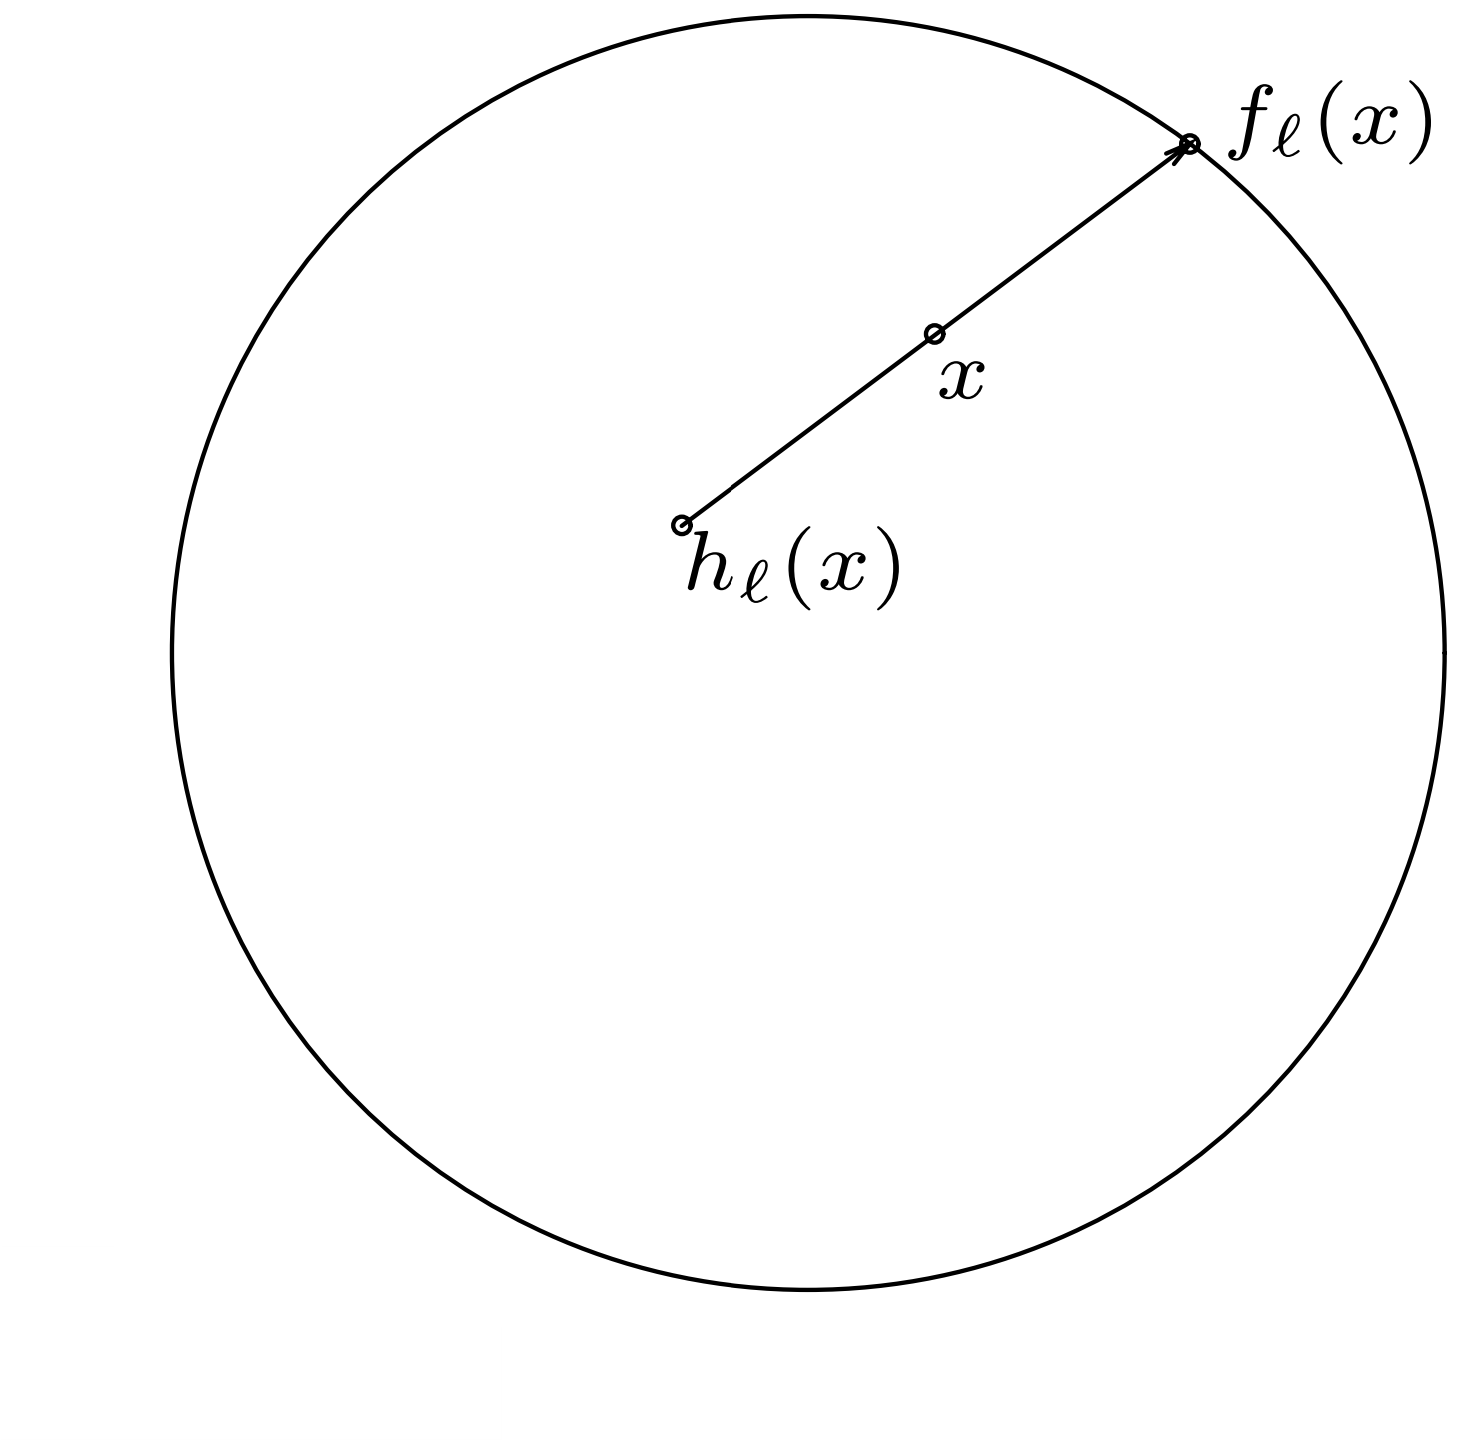
\includegraphics[scale=0.33]{Ralph Howard Circle Diagram.png}}
	\end{tabular}

	Note $\|h_\ell(x) + t(x - h_\ell(x))\|_2^2 = \|h_\ell(x)\|_2^2 + 2t(h_\ell(x) \cdot (x - h_\ell(x))) + t^2\|x - h_\ell(x)\|_2^2$. Therefore, we need to solve the following quadratic equation:

	{\centering $(\|h_\ell(x)\|_2^2 - 1) + 2t(h_\ell(x) \cdot (x - h_\ell(x))) + t^2\|x - h_\ell(x)\|_2^2 = 0$. \newpage\par}

	So, apply quadratic formula to get that:
	$$t = \frac{-(h_\ell(x) \cdot (x - h_\ell(x))) \pm \sqrt{(h_\ell(x) \cdot (x - h_\ell(x)))^2 - (\|h_\ell(x)\|_2^2 - 1)\|x - h_\ell(x)\|_2^2}}{\|x - h_\ell(x)\|_2^2}$$\retTwo

	Now since $\|h_\ell(x)\|_2 \leq 1$, we have that:
	
	{\centering$(y \cdot (x - h_\ell(x)))^2 - (\|h_\ell(x)\|_2^2 - 1)\|x - h_\ell(x)\|_2^2 \geq (h_\ell(x) \cdot (x - h_\ell(x)))^2 \geq 0$ \retTwo\par}

	Hence, any $t$ solving our quadratic will be real valued. Also importantly, since the line\\ passing through $h_\ell(x)$ and $x$ intercepts $\overline{B^{n}}$ in more than one place (namely $h_\ell(x)$ and $x$), that line must intercept $S^{n-1}$ in two places. Hence, two values of $t$ must satisfy our quadratic. And this proves that the long expression under the radical never equals $0$.\retTwo

	Finally, the root we want is specifically the greater of the two. So, we set:
	
	{\centering$T(x) \coloneqq \frac{-(h_\ell(x) \cdot (x - h_\ell(x))) + \sqrt{(h_\ell(x) \cdot (x - h_\ell(x)))^2 - (\|h_\ell(x)\|_2^2 - 1)\|x - h_\ell(x)\|_2^2}}{\|x - h_\ell(x)\|_2^2}$.\retTwo\par}
	
	And importantly, $T(x)$ is a smooth real-valued function.\retTwo

	But now $f_\ell(x) = h_\ell(x) = T(x)(x - h_\ell(x))$ is smooth, maps all of $\overline{B^n}$ into $S^{n-1}$, and fixes $S^{n-1}$. This violates lemma 1. So, the premise that $h_\ell$ had no fixed point has to be false.\retTwo

	To finish off our proof, for each $\ell \in \mathbb{N}$ pick $x_\ell$ such that $h_\ell(x_\ell) = x_\ell$. Since $\overline{B^n}$ is compact, we know that there is a convergent subsequence $\{x_{\ell_k}\}_{k \in \mathbb{N}}$ converging to $x^{(0)} \in \overline{B^n}$. And now since $\sup_{x \in \overline{B^n}} \|h_\ell(x) - f(x)\|_2 \to 0$, we have that:

	{\centering $f(x^{(0)}) = \lim_{k \to \infty}h_{\ell_{k}}(x_{\ell_{k}}) = \lim_{k \to \infty}x_{\ell_k} = x^{(0)}$. $\blacksquare$\retTwo\par}
\end{myIndent}

\hTwo While I'm at it, here is Howard's theorem 2:\retTwo

\exTwo\ul{Corollary:} There is no continuous map $f : \overline{B^n} \to S^{n-1}$ with $f(x) = x$ for all $x \in S^{n-1}$.
\begin{myIndent}\exThreeP
	Proof:\\
	Assume such a map exists and let $g(x) = -f(x)$. Then $g$ is also a map from $\overline{B^n}$ to\\ $S^{n-1} \subseteq \overline{B^n}$. By the Brouwer fixed point theorem $g$ must have a fixed point $y \in \overline{B^n}$. But if $y \in S^{n-1}$, then $g(y) = -f(y) = -y \neq y$. Meanwhile, $g(y) \notin B^n$ for all $y \in B^n$. So, $g$ can't have a fixed point. This is a contradiction. $\blacksquare$\retTwo
\end{myIndent}

\hTwo\mySepTwo

\hypertarget{math 200a lecture 8}{\blect{Math 200a (don't know what lecture)}}

\exTwo\ul{Lemma:} The standard S.E.S. (where $N \lhd G$):
% https://q.uiver.app/#q=WzAsNSxbMCwwLCJcXHsxXFx9Il0sWzEsMCwiTiJdLFsyLDAsIkciXSxbMywwLCJHL04iXSxbNCwwLCJcXHsxXFx9Il0sWzAsMV0sWzEsMiwiaSIsMCx7InN0eWxlIjp7InRhaWwiOnsibmFtZSI6Imhvb2siLCJzaWRlIjoidG9wIn19fV0sWzIsMywiXFxwaSIsMCx7InN0eWxlIjp7ImhlYWQiOnsibmFtZSI6ImVwaSJ9fX1dLFszLDRdXQ==
\[\begin{tikzcd}
	{\{1\}} & N & G & {G/N} & {\{1\}}
	\arrow[from=1-1, to=1-2]
	\arrow["i", hook, from=1-2, to=1-3]
	\arrow["\pi", two heads, from=1-3, to=1-4]
	\arrow[from=1-4, to=1-5]
\end{tikzcd}\]
splits iff there exists $H < G$ such that $HN = G$ and $H \cap N = \{1\}$.

\begin{myIndent}\exThreeP
	$(\Longrightarrow)$\\
	Assuming that it splits, we get a group homomorphism $f : G/N \to G$ such that\\ $\forall x \in G,\gap f(xN)N = xN$. If $xN \in \ker(f)$ then $xN = f(xN)N = N$. So, $f$ is\\ injective. And hence, by letting $H \coloneqq \myIm(f)$ we get that $H < G$ and that $H \cong G/N$\\ (by the first isomorphism theorem).
	\begin{itemize}
		\item If $x \in H \cap N$, then we claim that $x = 1_G$.\newpage
		\begin{myIndent}\exPPP
			Why?\\
			If $x \in H$ then $x = f(x^\prime N)$ for some $x^\prime \in G$. And hence:
			
			{\centering$xN = f(x^\prime N)N = x^\prime N$.\retTwo\par}
			
			But if also $x \in N$, then $xN = N$. So $x^\prime N = N$ and in turn:
			
			{\centering$x = f(x^\prime N) = 1_G$.\retTwo\par}
		\end{myIndent}

		\item For all $x \in G$ there exists $h \in H$ and $n \in N$ with $x = hn$.
		\begin{myIndent}\exPPP
			Why?\\
			We know for all $xN \in G/N$ that there exists $h = f(xN) \in H$ such that $hN = xN$. In turn, for any $x \in G$ we can find a coset $hN$ containing $x$ where $h \in H$. So, $G = HN$.\retTwo
		\end{myIndent}
	\end{itemize}

	$(\Longleftarrow)$\\
	By the second isomorphism theorem, we know that $(HN)/N \cong H/(H \cap N)$. Also, by our assumptions, we know that $G/N \cong (HN)/N$ and that $H/(H \cap N) \cong H$. So, let $\theta(hN) = h$ for all $h \in H$. (This is just the isomorphism going from $G/N$ to $H$ that would have been defined by our isomorphism theorem).\retTwo

	\begin{myIndent}\pracTwo
		If you really don't trust that this is an isomorphism, note that since $HN = G$ we know for all $xN \in G / N$ there exists $h \in H$ with $xN = hN$. Also, if $h_1N = h_2N$, then $h_2^{-1}h_1 = n^{-1}$ for some $n \in N$. And since $H \cap N = \{1\}$, this means that $h_2^{-1}h_1 = 1$. So, $h_2 = h_1$. Hence, $\theta$ is a well-defined map from $G/N$ to $H$.\retTwo

		Now the rest of the proof that $\theta$ is a group isomorphism is trivial\dots\retTwo
	\end{myIndent}

	Next, define $f = i \circ \theta$ so that the diagram below commutes.
	% https://q.uiver.app/#q=WzAsMyxbMCwwLCJHL04iXSxbMSwwLCJIIl0sWzIsMCwiRyJdLFsxLDIsImkiLDAseyJzdHlsZSI6eyJ0YWlsIjp7Im5hbWUiOiJob29rIiwic2lkZSI6InRvcCJ9fX1dLFswLDEsIlxcdGhldGEiXSxbMCwyLCJmIiwyLHsiY3VydmUiOjJ9XV0=
	\[\begin{tikzcd}
		{G/N} & H & G
		\arrow["\theta", from=1-1, to=1-2]
		\arrow["f"', curve={height=12pt}, from=1-1, to=1-3]
		\arrow["i", hook, from=1-2, to=1-3]
	\end{tikzcd}\]

	Clearly $g$ is a group homomorphism and we claim that $f$ splits our S.E.S.
	\begin{myIndent}\exPPP
		Why?
		For any $xN \in G / N$ we have that $\theta(xN) \in H$. Thus $\theta(\theta(xN)N) = \theta(xN)$. And since $\theta$ is injective, we must have that $\theta(xN)N = xN$. $\blacksquare$\retTwo
	\end{myIndent}
\end{myIndent}

\hTwo So now that we have a condition for when our  standard S.E.S. splits in terms of the\\ existence of a group $H < G$ with certain properties. Is there a way to give the set $N \times H$ a group structure such that the obvious bijection $\phi(n, h) = nh$ is a group isomorphism and also the below diagram commutes?\\ [-20pt]

% https://q.uiver.app/#q=WzAsMTAsWzAsMCwiXFx7MVxcfSJdLFswLDEsIlxcezFcXH0iXSxbMSwwLCJOIl0sWzEsMSwiTiJdLFsyLDEsIk4gXFx0aW1lcyBIIl0sWzIsMCwiRyJdLFszLDEsIkgiXSxbMywwLCJHL04iXSxbNCwxLCJcXHsxXFx9Il0sWzQsMCwiXFx7MVxcfSJdLFsxLDNdLFswLDJdLFszLDIsIlxcbXlJZCJdLFsyLDUsImkiLDAseyJzdHlsZSI6eyJ0YWlsIjp7Im5hbWUiOiJob29rIiwic2lkZSI6InRvcCJ9fX1dLFszLDRdLFs0LDZdLFs1LDcsIlxccGkiLDAseyJvZmZzZXQiOi0xfV0sWzYsNywiXFxwaSBcXGNpcmMgaSIsMl0sWzcsNSwiZiIsMCx7Im9mZnNldCI6LTF9XSxbNiw4XSxbNyw5XSxbNCw0LCIobixoKSIsMix7Im9mZnNldCI6LTEsInJhZGl1cyI6LTEsInN0eWxlIjp7ImJvZHkiOnsibmFtZSI6Im5vbmUifSwiaGVhZCI6eyJuYW1lIjoibm9uZSJ9fX1dLFs0LDUsIj8iLDJdLFs1LDUsIm5oIiwwLHsib2Zmc2V0Ijo1LCJzdHlsZSI6eyJib2R5Ijp7Im5hbWUiOiJub25lIn0sImhlYWQiOnsibmFtZSI6Im5vbmUifX19XV0=
\[\begin{tikzcd}
	{\{1\}} & N & G & {G/N} & {\{1\}} \\
	{\{1\}} & N & {N \times H} & H & {\{1\}}
	\arrow[from=1-1, to=1-2]
	\arrow["i", hook, from=1-2, to=1-3]
	\arrow["\pi", shift left, from=1-3, to=1-4]
	\arrow["f", shift left, from=1-4, to=1-3]
	\arrow[from=1-4, to=1-5]
	\arrow[from=2-1, to=2-2]
	\arrow["\myId", from=2-2, to=1-2]
	\arrow[from=2-2, to=2-3]
	\arrow["{\phi}"', from=2-3, to=1-3]
	\arrow[from=2-3, to=2-4]
	\arrow["{\pi \circ i}"', from=2-4, to=1-4]
	\arrow[from=2-4, to=2-5]
\end{tikzcd}\]\retTwo

Since our diagram needs to commute, we must have that have that:

{\centering$\phi(n_1, h_1)\phi(n_2, h_2) = (n_1h_1)(n_2h_2) = nh_1n_2h_1^{-1}h_1h_2 = \phi(n_1h_1n_2h_1^{-1}, h_1h_2)$\retTwo\par}

And this now motivates us to define the \udefine{semidirect product} of $N$ and $H$.\newpage

Let $H$ and $N$ be groups (right now we won't assume they are subgroups of another group) and let $f: H \to \Aut(N)$ be a group homomorphism. Then define the operation:

{\centering $(n_1, h_1) \cdot (n_2, h_2) = (n_1(f(h_1))(n_2), h_1h_2)$ \retTwo\par}

This turns $(N \times H, \cdot)$ into a group which we denote as $N \rtimes_f H$ to distinguish it from the\\ \udefine{direct product} of $N$ and $H$ (which has group product $(n_1, h_1) \cdot (n_2, h_2) = (n_1n_2, h_1h_2)$).
\begin{myDindent}\myComment
	Proving that $N \rtimes_f H$ is a group would be boring and it's already in math 100a notes from last Fall.\retTwo
\end{myDindent}

Alireza (the professor teaching this class) likes to use the shorthand $\underline{n} \coloneqq (n, 1)$ and\\ $\underline{h} \coloneqq (1, h)$. Note that $\theta_1 : N \to N \rtimes_f H$ given by $n \mapsto \underline{n}$ and $\theta : H \to N \rtimes_f H$ given\\ by $h \mapsto \underline{h}$ are injective group homomorphisms. Furthermore, the map $\theta_2 : N \rtimes_f H \to H$\\ given by $(n, h) \mapsto h$ is a surjective group homomorphism.
\begin{myDindent}\myComment
	I'm again skipping proving these since it's just a lot of symbol moving.\retTwo
\end{myDindent}

\exTwo\ul{Corollary:} The following is a splitting S.E.S. (which we call a \udefine{standard splitting S.E.S.}):
% https://q.uiver.app/#q=WzAsNSxbMCwwLCJcXHsxXFx9Il0sWzEsMCwiTiJdLFsyLDAsIk4gXFxydGltZXNfZiBIIl0sWzMsMCwiSCJdLFs0LDAsIlxcezFcXH0iXSxbMCwxXSxbMSwyLCJcXHRoZXRhXzEiXSxbMiwzLCJcXHRoZXRhXzIiLDAseyJvZmZzZXQiOi0xfV0sWzMsNF0sWzMsMiwiXFx0aGV0YSIsMCx7Im9mZnNldCI6LTF9XV0=
\[\begin{tikzcd}
	{\{1\}} & N & {N \rtimes_f H} & H & {\{1\}}
	\arrow[from=1-1, to=1-2]
	\arrow["{\theta_1}", from=1-2, to=1-3]
	\arrow["{\theta_2}", shift left, from=1-3, to=1-4]
	\arrow["\theta", shift left, from=1-4, to=1-3]
	\arrow[from=1-4, to=1-5]
\end{tikzcd}\]

\hTwo\mySepTwo

\exTwo\ul{Theorem:} Suppose \\ [-36pt]
% https://q.uiver.app/#q=WzAsNSxbMCwwLCJcXHsxXFx9Il0sWzEsMCwiTiJdLFsyLDAsIk4gXFxydGltZXNfZiBIIl0sWzMsMCwiSCJdLFs0LDAsIlxcezFcXH0iXSxbMCwxXSxbMSwyLCJcXHRoZXRhXzEiXSxbMiwzLCJcXHRoZXRhXzIiLDAseyJvZmZzZXQiOi0xfV0sWzMsNF0sWzMsMiwiXFx0aGV0YSIsMCx7Im9mZnNldCI6LTF9XV0=
\[\begin{tikzcd}
	{\{1\}} & G_1 & {G_2} & G_3 & {\{1\}}
	\arrow[from=1-1, to=1-2]
	\arrow["{\theta_1}", from=1-2, to=1-3]
	\arrow["{\theta_2}", shift left, from=1-3, to=1-4]
	\arrow["\theta", shift left, from=1-4, to=1-3]
	\arrow[from=1-4, to=1-5]
\end{tikzcd}\]

\phantom{.}\\[-36pt]\phantom{aaaaaaaaaaaaaaaaaaaaaaaaaaaaaaaaaaaaaaaaaaaaaaaaaaaaaaaaaaa} is a splitting S.E.S.\\ [10pt]

Then by letting $f: G_3 \to \Aut(G_1)$ be given by $(f(x_3))(x_1) \coloneqq \theta^{-1}_1(\theta(x_3)\theta_1(x_1)\theta(x_3)^{-1})$ and $\phi: G_1 \rtimes_f G_3 \to G_2$ be given by $\phi(x_1, x_3) \coloneqq \theta_1(x_1)\theta(x_3)$ we have that the following is an isomorphism of S.E.S.s.:
% https://q.uiver.app/#q=WzAsMTAsWzAsMCwiXFx7MVxcfSJdLFswLDEsIlxcezFcXH0iXSxbMSwwLCJHXzIiXSxbMSwxLCJHXzEiXSxbMiwxLCJHXzEgXFxydGltZXNfZiBHXzMiXSxbMiwwLCJHXzIiXSxbMywxLCJHXzMiXSxbMywwLCJHXzMiXSxbNCwxLCJcXHsxXFx9Il0sWzQsMCwiXFx7MVxcfSJdLFsxLDNdLFswLDJdLFszLDIsIlxcbXlJZCJdLFsyLDUsIlxcdGhldGFfMSJdLFszLDQsImdfMSBcXG1hcHN0b1xcdW5kZXJsaW5le2dfMX0iLDJdLFs0LDYsIihnXzEsIGdfMylcXG1hcHN0byBnXzMiLDJdLFs1LDcsIlxcdGhldGFfMiJdLFs2LDcsIlxcbXlJZCIsMl0sWzYsOF0sWzcsOV0sWzQsNSwiXFxwaGkiLDJdXQ==
\[\begin{tikzcd}
	{\{1\}} & {G_1} & {G_2} & {G_3} & {\{1\}} \\
	{\{1\}} & {G_1} & {G_1 \rtimes_f G_3} & {G_3} & {\{1\}}
	\arrow[from=1-1, to=1-2]
	\arrow["{\theta_1}", from=1-2, to=1-3]
	\arrow["{\theta_2}", from=1-3, to=1-4]
	\arrow[from=1-4, to=1-5]
	\arrow[from=2-1, to=2-2]
	\arrow["\myId", from=2-2, to=1-2]
	\arrow["{g_1 \mapsto\underline{g_1}}"', from=2-2, to=2-3]
	\arrow["\phi"', from=2-3, to=1-3]
	\arrow["{(g_1, g_3)\mapsto g_3}"', from=2-3, to=2-4]
	\arrow["\myId"', from=2-4, to=1-4]
	\arrow[from=2-4, to=2-5]
\end{tikzcd}\]

\begin{myIndent}\exThreeP
	Proof:\\
	First we show $f(x_3) \in \Aut(G_1)$ for all $x_3 \in G_3$:
	\begin{itemize}
		\item Firstly, because $\myIm(\theta_1) = \ker(\theta_2)$ is a normal subgroup, we know that\\ $\theta(x_3)\theta_1(x_1)\theta(x_3)^{-1}$ is also in $\myIm(\theta_1)$. Also, since $\theta_1$ is injective, we know that\\ there is a unique element in $\theta^{-1}(y)$ for any $y \in \myIm(\theta_1)$. So, $(f(x_3))$ is a well-\\defined function.\retTwo
		
		\item Let $x_1, y_1 \in G_1$ and $x_3 \in G_3$. Then:
		
		{\centering\begin{tabular}{l}
			$(f(x_3))(x_1) \cdot (f(x_3))(y_1) = \theta_1^{-1}(\theta(x_3)\theta_1(x_1)\theta(x_3)^{-1})\theta_1^{-1}(\theta(x_3)\theta_1(y_1)\theta(x_3)^{-1})$\\ [6pt]
			$\phantom{(f(x_3))(x_1) \cdot (f(x_3))(y_1)} = \theta_1^{-1}((\theta(x_3)\theta_1(x_1)\theta(x_3)^{-1})( \theta(x_3)\theta_1(y_1)\theta(x_3)^{-1}))$\\ [6pt]
			$\phantom{(f(x_3))(x_1) \cdot (f(x_3))(y_1)} = \theta_1^{-1}(\theta(x_3)\theta_1(x_1)\theta_1(y_1)\theta(x_3)^{-1})$\\ [6pt]
			$\phantom{(f(x_3))(x_1) \cdot (f(x_3))(y_1)} = (f(x_3))(x_1y_1)$\\ [6pt]
		\end{tabular}\newpage\par}

		This shows that $(f(x_3))$ is a group homomorphism.\retTwo

		\item Since $\theta_1$ is injective, we know that if $\theta^{-1}(y) = 1$ (where $y \in \myIm(\theta_1)$), then\\ $y = 1$. Hence if $(f(x_3))(x_1) = 1$ then $\theta(x_3)\theta_1(x_1)\theta(x_3)^{-1} = 1$. But then\\ $\theta_1(x_1) = \theta(x_3)^{-1}\theta(x_3) = 1$. So by using the injectivity of $\theta_1$ again have that\\ $x_1 = 1$. And this proves that $(f(x_3))$ is injective.\retTwo
		
		\item Finally, if $x_1 \in G_1$, then let $y_1 = \theta^{-1}(\theta(x_3)^{-1}\theta(x_1)\theta(x_3))$. Then it is easy to see\\ that $\theta(y_1) = x_1$. So, $(f(x_3))$ is surjective.\retTwo
	\end{itemize}

	Next we show that $f$ is a group homomorphism:
	\begin{itemize}
		\item[\phantom{}] Fix $x_1 \in G_1$ and let $x_3, y_3 \in G_3$. Then:
		
		{\centering\begin{tabular}{l}
			$(f(y_3))((f(x_3))(x_1)) = \theta_1^{-1}(\theta(y_3)\theta_1((f(y_3))(x_1))\theta(y_3)^{-1})$\\ [6pt]
			$\phantom{(f(y_3))((f(x_3))(x_1))} = \theta_1^{-1}(\theta(y_3)\theta_1(\theta_1^{-1}(\theta(x_3)\theta_1(x_1)\theta(x_3)^{-1}))\theta(y_3)^{-1})$\\ [6pt]
			$\phantom{(f(y_3))((f(x_3))(x_1))} = \theta_1^{-1}(\theta(y_3)\theta(x_3)\theta_1(x_1)\theta(x_3)^{-1}\theta(y_3)^{-1})$\\ [6pt]
			$\phantom{(f(y_3))((f(x_3))(x_1))} = \theta_1^{-1}(\theta(y_3 x_3)\theta_1(x_1)\theta(y_3x_3)^{-1})$\\ [6pt]
			$\phantom{(f(y_3))((f(x_3))(x_1))} = (f(y_3x_3))(x_1)$\\ [6pt]
		\end{tabular}\retTwo\par}

		And this proves that $f(y_3) \circ f(x_3) = f(y_3x_3)$. So $f$ is a group homomorphism.\retTwo
	\end{itemize}

	With that, we now have a well-defined semidirect product $G_1 \rtimes_f G_3$. So, we next show that the function $\phi$ we defined before is a group homomorphism:
	\begin{itemize}
		\item[\phantom{}] Note that for any $x_1, y_1 \in G_1$ and $x_3, y_3 \in G_3$:
		
		{\centering\begin{tabular}{l}
			$\phi((x_1, x_3) \cdot (y_1, y_3)) = \phi((x_1(f(x_3)(y_1), x_3y_3)))$\\ [6pt]
			$\phantom{\phi((x_1, x_3) \cdot (y_1, y_3))} = \theta_1(x_1(f(x_3))(y_1))\theta(x_3y_3)$\\ [6pt]
			$\phantom{\phi((x_1, x_3) \cdot (y_1, y_3))} = \theta_1(x_1)\theta_1((f(x_3))(y_1))\theta(x_3)\theta(y_3)$\\ [6pt]
			$\phantom{\phi((x_1, x_3) \cdot (y_1, y_3))} = \theta_1(x_1)\theta(x_3)\theta_1(y_1)\theta(x_3)^{-1}\theta(x_3)\theta(y_3)$\\ [6pt]
			$\phantom{\phi((x_1, x_3) \cdot (y_1, y_3))} = \theta_1(x_1)\theta(x_3)\theta_1(y_1)\theta(y_3) = \phi((x_1, x_3))\phi((y_1, y_3))$.
		\end{tabular}\retTwo\par}
	\end{itemize}

	Finally, if our proposed diagram actually commutes, then we can apply the short five lemma to get that $\phi$ is a group isomorphism. And then we will be done.
	\begin{itemize}
		\item $\phi(\underline{x_1}) = \phi(x_1, 1) = \theta_1(x_1)\theta(1) = \theta_1(x_1)$. Thus the first square commutes.\retTwo
		
		\item Since $\myIm(\theta_1) = \ker(\theta_2)$, we know that $\theta_2(\theta_1(x_1)) = 1$ for all $x_1 \in G_1$. Also, recall that $\theta_2(\theta(x_3)) = x_3$. Therefore:
		
		{\centering$\theta_2(\phi((x_1, x_3))) = \theta_2(\theta_1(x_1)\theta(x_3)) = \theta_2(\theta_1(x_1))\theta_2(\theta(x_3)) = x_3$\retTwo\par}

		And this proves the second square commutes. $\blacksquare$\retTwo
	\end{itemize}
\end{myIndent}

\pracOne\mySepTwo

I somehow just realized something really helpful that I want to write down:\newpage

\ul{Proposition:} Suppose we have the following diagram:
% https://q.uiver.app/#q=WzAsNCxbMCwwLCJBIl0sWzEsMCwiQiJdLFswLDEsIkMiXSxbMSwxLCJEIl0sWzIsMCwiXFx0aGV0YSIsMCx7Im9mZnNldCI6LTF9XSxbMCwyLCJcXHRoZXRhXnstMX0iLDAseyJvZmZzZXQiOi0xfV0sWzMsMSwiXFxwaGkiLDAseyJvZmZzZXQiOi0xfV0sWzEsMywiXFxwaGleey0xfSIsMCx7Im9mZnNldCI6LTF9XSxbMCwxLCJmIl0sWzIsMywiZyIsMl1d
\[\begin{tikzcd}[sep=large]
	A & B \\
	C & D
	\arrow["f", from=1-1, to=1-2]
	\arrow["{\theta^{-1}}", shift left, from=1-1, to=2-1]
	\arrow["{\phi^{-1}}", shift left, from=1-2, to=2-2]
	\arrow["\theta", shift left, from=2-1, to=1-1]
	\arrow["g"', from=2-1, to=2-2]
	\arrow["\phi", shift left, from=2-2, to=1-2]
\end{tikzcd}\]

If $\theta f = g\phi$, then $f\phi^{-1} = \theta^{-1} g$. (i.e. if the vertical arrows are isomorphisms, then we only need to check if going around one way commutes).
\begin{myIndent}\pracTwo
	Proof:\\
	$f\phi^{-1} = (\theta^{-1}\theta) f \phi^{-1} = \theta^{-1}(\theta f) \phi^{-1} = \theta^{-1}(g \phi)\phi^{-1} = \theta^{-1} g (\phi \phi^{-1}) = \theta^{-1} g$. $\blacksquare$\retTwo
\end{myIndent}

\mySepTwo

\hTwo\dispDate{10/20/2025}

\hypertarget{math 220a lecture 9}{\blect{Math 220a (I don't know which lecture):}}\retTwo

If $G \subseteq \mathbb{C}$ is a region and $f: G \to \mathbb{C}$ is a continuous functions such that $z = \exp(f(z))$ for all $z \in G$, then $f$ is a \udefine{branch of the logarithm}.\retTwo

For the most important (or "principle") branch of the logarithm, let:

{\centering$G = \mathbb{C} - \{z : \ima{z} = 0 \text{ and } \rea{z} \leq 0\}$.\retTwo\par}

Clearly $G$ is connected and open, and each $z \in G$ can be uniquely represented as  $z = |z|e^{i\theta}$ for some $\theta \in (-\pi, +\pi)$. So, for all $re^{i\theta} \in G$ (where $0 < r$ and $\theta \in (-\pi, \pi)$) we define:

{\centering$\Log(re^{i\theta}) = \log(r) + i\theta$\par}

\begin{myTindent}\myComment
	(\dots where $\log$ refers to the normal real logarithm while $\Log$ refers to the\\ \udefine{principle branch} of the complex logarithm).\retTwo
\end{myTindent}

\Hstatement\blab{Exercise III.2.9:} Suppose $\{z_n\}_{n \in \mathbb{N}}$ is a sequence in $G$ converging to $z$ and $z_n = r_ne^{i\theta_n}$ and\\ $z = re^{i\theta}$ where $r, r_n > 0$ and $\theta, \theta_n \in (-\pi, \pi)$. Then $r_n \to r$ and $\theta_n \to \theta$.
\begin{myIndent}\HexOne
	Proof:\\
	$|\cdot|$ is continuous (as is seen by reverse triangle inequality). Therefore, since $z_n \to z$, we know that $r_n = |z_n| \to |z| = r$ as $n \to \infty$. As a consequence, since $r_n, r \neq 0$ for any $r$, we can say that $e^{i\theta_n} = \frac{z_n}{r_n} \to \frac{z}{r} = e^{i\theta}$ as $n \to \infty$.\retTwo

	Finally note that $e^{i\theta}$ is in the interior of either $\{z \in \mathbb{C} : \rea{z} > 0\}$, $\{z \in \mathbb{C} : \ima{z} > 0\}$, or $\{z \in \mathbb{C} : \ima{z} < 0\}$. Thus we must have that $e^{i\theta_n}$ is eventually in one of those open sets, which in turn means $\theta_n$ is eventually in $[-\sfrac{\pi}{2}, \sfrac{\pi}{2}]$, $[0, \pi]$, or $[-\pi, 0]$. In either of those cases, call the interval $\theta_n$ is eventually in $K$.\retTwo

	Now $f : K \to \myIm(f)$ given by $f^{it}$ is a bijective function from a compact space to a metric space. Hence $f^{-1} : \myIm(f) \to K$ is also continuous. So, the fact that $f(\theta_n) \to f(\theta)$ means that $\theta_n = f^{-1}(f(\theta_n)) \to f^{-1}(f(\theta)) = \theta$. $\blacksquare$\retTwo
\end{myIndent}

\blab{Corollary:} $\Log : G \to \mathbb{C}$ is continuous.\newpage

\exTwo\ul{(Conway) Proposition 2.20:} Let $G$ and $\Omega$ be open subsets of $\mathbb{C}$ and suppose that $f: G \to \mathbb{C}$ and $g : \Omega \to \mathbb{C}$ are continuous functions such that $f(G) \subseteq \Omega$ and $g(f(z)) = z$ for all $z \in G$. If $g$ is differentiable and $g^\prime \neq 0$, then $f$ is differentiable and $f^\prime(z) = \frac{1}{g^\prime(f(z))}$.
\begin{myIndent}\exThreeP
	Proof:\\
	Fix $a \in G$ and let $h \in \mathbb{C}$ such that $h \neq 0$ and $a + h \in G$. Then $g(f(a)) = a$ and\\ $a + h = g(f(a + h))$ implies that $f(a) \neq f(a + h)$. So:

	{\centering $1 = \frac{a + h - a}{h} = \frac{g(f(a + h)) - g(f(a))}{h} = \frac{g(f(a + h)) - g(f(a))}{f(a + h) - f(a)}\cdot\frac{f(a + h) - f(a)}{h}$ \retTwo\par}

	And now we have that $\lim_{h \to 0}\frac{f(a + h) - f(a)}{h} = \left(\lim_{h \to \infty} \frac{g(f(a + h)) - g(f(a))}{f(a + h) - f(a)}\right)^{-1}$.\retTwo

	But since $|f(a + h) - f(a)| \to 0$ as $h \to 0$ (since $f$ is continuous) and $g$ is differentiable, we know that:

	{\centering$\lim_{h \to \infty} \frac{g(f(a + h)) - g(f(a))}{f(a + h) - f(a)} = g^\prime(f(a))$\retTwo\par}

	And this proves that $f^\prime(a)$ exists and equals $\frac{1}{g^\prime(f(a))}$.

	\begin{myIndent}\myComment
		Side note: In this case we also have that $f^\prime$ is as smooth as $g^\prime$ is.\retTwo
	\end{myIndent}
\end{myIndent}

\ul{(Conway) Corollary 2.21:} A branch of the logarithm is holomorphic and it's derivative\\ is $z^{-1}$.
\begin{myIndent}\exThreeP
	Proof:\\
	If $G \subseteq \mathbb{C}$ is a region and $f: G \to \mathbb{C}$ is a branch of the logarithm, then\\ $f^\prime(z) = (\exp^\prime(f(z)))^{-1} = (\exp(f(z)))^{-1} = z^{-1}$. $\blacksquare$\retTwo
\end{myIndent}

\pracOne\mySepTwo

A while ago I wrote down \inLinkRap{Cauchy-Riemann equations theorem}{a theorem} concerning the \udefine{Cauchy-Rieman equations}. But I never actually proved  one of the proof directions. So I'd like to do that now.\retTwo

\ul{Statement:} If $G$ is a region of $\mathbb{C} \cong \mathbb{R}^2$, and:\\ [-20pt]

{\center$f(x + iy) = f((x, y)) = (u(x, y), v(x, y)) \in C^1(G)$\\ [6pt]\par}

with $u_x = v_y$ and $v_x = -u_y$, then $f$ is holomorphic.

\begin{myIndent}\pracTwo
	Proof:\\
	Denote $r$ to be the common value of $u_x$ and $v_y$, and similarly define $s$ to be the common value of $v_x$ and $-u_y$. Then:

	{\centering $\begin{pmatrix}
	r & -s \\ s & r
	\end{pmatrix}\begin{pmatrix}
	h \\ k
	\end{pmatrix} \cong rh - sk + i(sh + rk) = (r + is)(h + ik)$ \retTwo\par}

	Now since $f \in C^1(G)$, we know that:

	{\centering\begin{tabular}{l}
		$0 = \lim\limits_{h + ik \to 0}\frac{|f(x + iy + h + ik) - f(x + iy) - (r + is)(h + ik)|}{|h + ik|} = \lim\limits_{h + ik \to 0}\left|\frac{f(x + iy + h + ik) - f(x + iy) - (r + is)(h + ik)}{h + ik}\right|$ \\ [8pt]
		$\phantom{0 = \lim\limits_{h + ik \to 0}\frac{|f(x + iy + h + ik) - f(x + iy) - (r + is)(h + ik)|}{|h + ik|}} = \lim\limits_{h + ik \to 0}\left|\frac{f(x + iy + h + ik) - f(x + iy)}{h + ik} - (r + is)\right|$
	\end{tabular}\retTwo\par}
	
	And thus $f^\prime(x + iy)$ is well defined with:

	{\centering $f^\prime(x + iy) = \lim\limits_{h + ik \to 0} \frac{f(x + iy + h + ik) - f(x + iy)}{h + ik} = r + is$. $\blacksquare$\newpage\par}
\end{myIndent}

\hTwo Suppose $f(x, y) = (u(x, y), v(x, y))$ has continuous second derivatives and satisfies\\ the Cauchy-Riemann equations. Then by differentiating a second time we get that:

{\centering $\frac{\partial^2 u}{\partial x^2} = \frac{\partial^2 v}{\partial x \partial y}$ and $\frac{\partial^2 v}{\partial y \partial x} = -\frac{\partial^2 u}{\partial y^2}$ \retTwo\par}

Hence, we get another partial differential equation:

{\centering $\frac{\partial^2 u}{\partial x^2} + \frac{\partial^2 u}{\partial y^2} = 0$ \retTwo\par}

Any function $u$ with continuous second derivatives satisfying the above differential\\ equation is said to be \udefine{harmonic}. Recalling that I proved last spring that complex\\ differentiable functions on a region are infinitely differentiable, we thus know that\\ if $G$ is a region of $\mathbb{C}$ and $f : G \to \mathbb{C}$ is holomorphic, then $\rea{f}$ is harmonic.\retTwo

On a related note, suppose $u : \mathbb{R}^2 \to \mathbb{R}$ is harmonic. Then can we find another function\\ $v : \mathbb{R}^2 \to \mathbb{R}$ such that $f(x + iy) = u(x, y) + iv(x, y)$ is holomorphic? The answer is\\ [-1pt] sometimes.
\begin{myIndent}\myComment
	As a side note, that hypothetical other function $v$ is called a \udefine{harmonic conjugate} of $u$.\retTwo
\end{myIndent}

\exTwo\ul{(Conway) Theorem 2.30:} Let $G$ be either all of $\mathbb{C}$ or an open disk. If $u : G \to \mathbb{R}$ is a\\ harmonic function (where we are identifying $\mathbb{C} \cong \mathbb{R}^2$), then $u$ has a harmonic conjugate.
\begin{myIndent}\exThreeP
	Proof:\\
	Without loss of generality assume the disk is centered at the origin. Also denote the radius of the disk as $R$ (where we allow $R = +\infty$). Now consider any function of the form:

	{\centering $v(x, y) = \int_0^y u_x(x, t)\df t + \psi(x)$ \retTwo\par}

	We focus on functions of this form because it is immediately clear from the fundamental theorem of calculus that $v_y(x, y) = u_x(x, y) + 0$. Also, modifying $\psi$ won't change what the $y$th. partial derivative of $v$ is. So, we now seek to find some function $\psi$ such that $v_x = -u_y$.\retTwo

	Note that since $u_x : \mathbb{R}^2 \to \mathbb{R}$ is continuous (since it is differentiable), we know by the extreme value theorem that for any $0 < r < R$ there is a constant $C_r > 0$ such that $u_x(x, y) \leq C_r$ when $\|x, y\|_2 \leq r$. Thus, we can apply the theorem on \inLinkRap{Generalization page 189}{page 189} to show that for any $y < r$ and $x < \sqrt{r^2 - y^2}$ that:

	{\centering\begin{tabular}{l}
		$v_x(x, y) = \frac{\partial}{\partial x}\int_0^y u_x(x, t)\df t + \frac{\df}{\df x}\psi(x)$ \\ [6pt]
		$\phantom{v_x(x, y)} = \int_0^y \frac{\partial}{\partial x} u_x(x, t) \df t + \frac{\df}{\df x}\psi(x) = -\int_0^y \frac{\df^2}{\df y^2}u(x, t) \df t + \frac{\df}{\df x}\psi(x)$\\ [6pt]
		$\phantom{v_x(x, y) = \int_0^y \frac{\partial}{\partial x} u_x(x, t) \df t + \frac{\df}{\df x}\psi(x)} = -u_y(x, y) + u_y(x, 0) + \frac{\df}{\df x}\psi(x)$\\ [6pt]
	\end{tabular}\retTwo\par}

	And by taking $r \to R$ we can say that $v_x(x, y) = -u_y(x, y) + u_y(x, 0) + \frac{\df}{\df x}\psi(x)$ for all $(x, y) \in G$. Therefore, we have that $v_x(x, y) = -u_y(x, y)$ iff $\frac{\df}{\df x}\psi(x) = -u_y(x, 0)$.\retTwo

	This clues us to fix $\psi$ so that:

	{\centering $v(x, y) \coloneqq \int_0^y u_x(x, t)\df t - \int_0^x u_y(s, 0)\df s$ \retTwo\par}

	And then $u$ and $v$ satisfy the Cauchy-Riemann equations. $\blacksquare$\retTwo
\end{myIndent}

\hTwo\newpage

\dispDate{10/22/2025}

Today I want to first quickly work through Folland chapter 11 section 1 on topological groups. I specifically want to do this because it is relevant to math 241.
\begin{myIndent}\myComment
	One quick bit of notation: If $A \subseteq G$ (where $A$ is not necessarily a subgroup), then I'll denote $A^{-1} = \{a^{-1} : a \in A\}$.\retTwo
\end{myIndent}

\exTwo\hypertarget{Folland proposition 11.1}{\ul{Proposition 11.1:}} Let $G$ be a topological group.
\begin{enumerate}
	\item[(a)] The topology of $G$ is translation invariant: If $U$ is open and $x \in G$, then $Ux$ and $xU$ are open.
	\begin{myIndent}\exThreeP
		This is just a result of translation being a continuous homeomorphism on $G$.\retTwo
	\end{myIndent}
	
	\item[(b)] For every neighborhood $U$ of $1$ there is a symmetric neighborhood $V$ of $1$ with $V \subseteq U$. (recall from \inLinkRap{page 238 symmetric generator definition}{page 238} what a symmetric subset of a group is).
	\begin{myIndent}\exThreeP
		Proof:\\ 
		Since inversion is continuous, we know that $U^{-1}$ also a neighborhood of $1$. So,\\ $U^{-1} \cap U$ is a neighborhood of $1$.\retTwo
	\end{myIndent}
	
	\item[(c)] For every neighborhood $U$ of $1$ there is a neighborhood $V$ of $1$ with $VV \subseteq U$.\\ (note that neighborhoods aren't necessarily subgroups but we still define\\ $AB = \{ab : a \in A, b\in B\}$). 
	\begin{myIndent}\exThreeP
		Proof:\\ 
		Since $1 \cdot 1 = 1 \in U$ and the group product is continuous, we know there are open sets $V_1, V_2 \subseteq G$ containing $1$ such that for all $a, b \in V_1 \times V_2$ we have that $ab \in U$. In particular, by taking $V = V_1 \cap V_2$ we have that $ab \in U$ for all $a, b \in V$ and that $V$ is an open set containing $1$.\retTwo
	\end{myIndent}
	
	\item[(d)] If $H$ is a subgroup of $G$, so is $\overline{H}$.
	
	\begin{myIndent}\exThreeP
		Proof:\\
		If $x, y \in \overline{H}$ then there are nets $\langle x_\alpha\rangle_{\alpha \in A}$ and $\langle y_\beta\rangle_{\beta \in B}$ contained in $H$ which converge to $x$ and $y$ respectively. But now $x_\alpha y_\beta \in H$ for all $\alpha \in A$ and $\beta \in B$. Hence, we may consider net $\langle x_\alpha y_\beta\rangle_{(\alpha, \beta) \in A \times B}$ where $A \times B$ is given the obvious partial ordering.\retTwo
		
		To see that this net converges to $xy$, consider any open neighborhood $U$ about $xy$ and note that since the group product is continuous, there are open sets $N_1, N_2$ around $x$ and $y$ respectively such that $x_\alpha y_\beta \in U$ whenever $x_\alpha \in N_1$ and $y_\beta \in N_2$. And since $x_\alpha \to x$ and $y_\beta \to y$, we can now easily find $(\alpha_0, \beta_0) \in A \times B$ such that $x_\alpha y_\beta \in U$ whenever $(\alpha, \beta) \gtrsim (\alpha_0, \beta_0)$.\retTwo

		And this proves that $xy \in \overline{H}$.\retTwo

		As for showing that $\overline{H}$ is closed under inversion, that is as simple as noting that\\ inversion is a homeomorphism and thus preserves set closures (see the first lemma\\ on \inLinkRap{page 318 lemma}{page 318}).\newpage
	\end{myIndent}
	
	\item[(e)] Every open subgroup of $G$ is also closed.
	\begin{myIndent}\exThreeP
		Proof:\\
		If $H$ is an open subgroup, then the cosets of $H$ are also open and so $H^\comp = \bigcup_{x \notin H} xH$ is open. This shows that $H$ is clopen.\retTwo
	\end{myIndent}
	
	\item[(f)] If $K_1, K_2$ are compact subsets of $G$, so is $K_1K_2$.
	\begin{myIndent}\exThreeP
		Proof:\\
		$K_1K_2$ is the image the compact set $K_1 \times K_2$ under the group composition map (which is continuous). $\blacksquare$\retTwo
	\end{myIndent}
\end{enumerate}

\hTwo If $f$ is a continuous function on a topological group $G$ and $y \in G$, we denote\\ $L_y f(x) = f(y^{-1}x)$ and $R_y f(x) = f(xy)$. This describes two group actions\\ $G \curvearrowright \Fun(G, X)$ (where $X$ is some other set).\retTwo

$f$ is called \udefine{left (or right) uniformly continuous} if for every $\varepsilon > 0$ there is a neighborhood\\ $V$ of $1_G$ such that $\|L_y f - f\|_u < \varepsilon$ (or $\|R_y f - f\|_u < \varepsilon$) for all $y \in V$.\retTwo

\exTwo\hypertarget{Folland Proposition 11.2}{\ul{Proposition 11.2:}} If $f \in C_c(G)$, then $f$ is left and right uniformly continuous.
\begin{myIndent}\exThreeP
	Proof:\\
	Folland only proves right uniform continuity. Thus, since the two proofs are analogous, I will only prove left uniform continuity.\retTwo

	Let $K = \supp(f)$ and suppose $\varepsilon > 0$. For each $x \in K$ there is a neighborhood $U_x$ of $1_G$ such that $|f(yx) - f(x)| < \sfrac{\varepsilon}{2}$ for all $y \in U_x$.
	\begin{myIndent}\exPPP
		Why? We know that $|f(x^\prime) - f(x)| < \sfrac{\varepsilon}{2}$ when $x^\prime$ is in some neighborhood\\ $N$ of $x$. Then in turn, since right translation is continuous, we know that\\ $U_x = \{y \in G : yx \in N\}$ is a neighborhood of $1_G$.\retTwo
	\end{myIndent}

	By proposition 11.1, we can in turn find a symmetric neighborhood $V_x \subseteq U_x$ of $1_G$ such\\ that $V_xV_x \subseteq U_x$. Hence, $V_x x$ is a neighborhoood of $x \in G$ with the property that if $g \in V_xV_x x$ then $|f(g) - f(x)| < \sfrac{\varepsilon}{2}$. (Note this also implies that if $g \in V_x x$ then $|f(g) - f(x)| < \sfrac{\varepsilon}{2}$).\retTwo

	Now since the $V_x x$ cover $K$ as we range over all $x \in K$ and $K$ is compact, we know that there are finitely many $x_1, \ldots, x_n$ such that $K \subseteq \bigcup_{j=1}^n V_{x_j} x_j$. So let $V = \bigcap_{j=1}^n V_{x_j}$ and note that $V$ is a symmetric neighborhood of $1_G$. We claim that $\|L_yf = f\|_u < \varepsilon$  for every $y \in V$.
	\begin{itemize}
		\item First suppose $x \in K$. Then $x \in V_{x_j}x_j$ for some $j$ and consequently we have\\ [-1pt] that $|f(x) - f(x_j)| < \sfrac{\varepsilon}{2}$. Also note that $xx_j^{-1} \in V_{x_j}$. So if $y \in V$ then\\ $y^{-1} x = y^{-1}(xx_j^{-1}) x_j \in V_{x_j}V_{x_j} x_{j}$ and we know that $|f(y^{-1}x) - f(x_j)| < \sfrac{\varepsilon}{2}$.\\ [1pt] Finally, by triangle inequality we have that:
		
		{\centering$|f(y^{-1}x) - f(x)| \leq |f(y^{-1}x) - f(x_j)| + |f(x_j) - f(x)| < \varepsilon$.\retTwo\par}

		\item Meanwhile suppose $x \notin K$. Then $f(x) = 0$. And if $y \in V$ then either $y^{-1}x \in K$ or $y^{-1}x \notin K$. For the latter case, we then trivially have that $f(y^{-1}x) = 0$ and so $|f(y^{-1} x) - f(x)| = 0 < \varepsilon$. As for if $y^{-1}x \in K$, then we know that $y^{-1} x \in V_{x_j} x_j$ for some $j$. And this means that $|f(y^{-1}x) - f(x_j)| < \sfrac{\varepsilon}{2}$.\newpage
		
		Also, $xx_j^{-1} = y (y^{-1}x x_j^{-1}) \in V_{x_j} V_{x_j} \subseteq U_{x_j}$. Hence:
		
		{\centering$|f(x_j)| = |f(x) - f(x_j)| = |f(xx_j^{-1}x_j) - f(x_j)| < \sfrac{\varepsilon}{2}$.\retTwo\par}

		So $|f(y^{-1}x) - f(x)| = |f(y^{-1}x)| \leq |f(y^{-1}x) - f(x_j)| + |f(x_j)| < \varepsilon$. $\blacksquare$\retTwo
	\end{itemize}
\end{myIndent}

\hTwo \hypertarget{idk reference 3 reversed}{I'll} continue with this on the weekend (see \inLinkRap{idk reference 3}{page 349}).\retTwo

\mySepTwo

\blect{More Math 220a Notes:}\retTwo

In this class we say a path $\gamma$ in a region $G \subseteq \mathbb{C}$ is a continuous function from a\\ closed interval $[a, b] \subseteq \mathbb{R}$ to $G$. We say a path $\gamma$ is \udefine{piecewise $C^1$} iff there exists\\ $a = t_0 < t_1 < \ldots < t_n = b$ such that $\gamma$ is $C^1$ on each subinterval $[t_{j-1}, t_j]$.\retTwo

If $\gamma_1, \gamma_2$ are $C^1$ paths, $z_0 = \gamma_1(t_1) = \gamma_2(t_2)$, and $\gamma_1^\prime(t_1) \neq 0$ and $\gamma_2^\prime(t_2) \neq 0$, then we define the angle between the paths $\gamma_1$ and $\gamma_2$ at $z_0$ to be $\arg \gamma_2^\prime(t_2) - \arg \gamma_1^\prime (t_1) \mMod{2\pi}$.\retTwo

Note that if $f : G \to \mathbb{C}$ is holomorphic and $\gamma_1, \gamma_2$ are $C^1$ paths in $G$, then $\sigma_1 = f \circ \gamma_1$ and $\sigma_2 = f \circ \gamma_2$ are also $C^1$ paths in $\mathbb{C}$. Now $\sigma^\prime_i(t) = f^\prime(\gamma_i(t))\gamma^\prime_i(t)$ which means that $\arg \sigma_i^\prime(t) = \arg(f^\prime(\gamma_i(t))) + \arg(\gamma_i^\prime(t))$ (if $f^\prime(\gamma_i(t)) \neq 0$ and $\gamma_i^\prime(t) \neq 0$). And consequently, if $\gamma_1$ intercepts $\gamma_2$ at some point (say $\gamma_1(t_1) = \gamma_2(t_2) = z_0$) and none of our derivatives are zero, then we have that $\sigma_1(t_1) = \sigma_2(t_2) = f(z_0)$ and:

{\centering\begin{tabular}{l}
	$\arg(\sigma_2^\prime(t_2)) - \arg(\sigma_1^\prime(t_1)) = \arg(f^\prime(z_0)) + \arg(\gamma_2^\prime(t_2)) - \arg(f^\prime(z_0)) - \arg(\gamma_1^\prime(t_1))$\\
	$\phantom{\arg(\sigma_2^\prime(t_2)) - \arg(\sigma_1^\prime(t_1))} = \arg(\gamma_2^\prime(t_2))- \arg(\gamma_1^\prime(t_1))$ 
\end{tabular}\retTwo\par}

In conclusion, we have the following theorem:
\begin{myIndent}\exTwo
	\ul{(Conway) Theorem III.3.4:} If $f : G \to \mathbb{C}$ is holomorphic then $f$ \udefine{preserves angles} at each point $z_0 \in G$ where $f^\prime(z_0) \neq 0$.\retTwo
\end{myIndent}

A function $f : G \to \mathbb{C}$ which has the above described angle preserving property at $a \in G$ and which also satisfies that $\lim_{z \to a} \left|\frac{f(z) - f(a)}{z - a}\right|$ exists is called a \udefine{conformal} at $a$. If $f$ is a bijection and $f$ is conformal at every point of $G$, then $f$ is called a \udefine{conformal map}.\retTwo

\mySepTwo

A function $S(z) = \frac{az + b}{cz + d}$ (where $ad - bc \neq 0$) is called a \udefine{Möbius transformation}.
\begin{itemize}
	\item Note that if $S(z)$ is a Möbius transformation, then $S^{-1}(z) = \frac{dz - b}{-cz + a}$ satisfies that $(da - (-b)(-c)) \neq 0$ and:
	
	{\centering $S(S^{-1}(z)) = \frac{a\frac{dz - b}{-cz + a} + b}{c\frac{dz - b}{-cz + a} + d} = \frac{a(dz - b) + b(a-cz)}{c(dz - b) + d(a - cz)} = \frac{adz - bc z}{- bc + ad} = z$ (if $z \neq \sfrac{a}{c}$)\retTwo
	$S^{-1}(S(z)) = \frac{d(\frac{az + b}{cz + d}) - b}{-c(\frac{az + b}{cz + d}) + a} = \frac{d(az + b) - b(cz + d)}{-c(az + b) + a(cz + d)} = \frac{ad z - bc z}{-bc + ad} = z$ (if $z \neq \sfrac{-d}{c}$).\retTwo\par}

	\item Suppose $T(z) = \frac{a_1z + b_1}{c_1 z + d_1}$ and $S(z) = \frac{a_2 z + b_2}{c_2 z + d_2}$, then:\newpage
	
	{\centering $(T \circ S)(z) =  \frac{a_1\frac{a_2 z + b_2}{c_2 z + d_2} + b_1}{c_1\frac{a_2 z + b_2}{c_2 z + d_2} + d_1} = \frac{a_1a_2 z + a_1 b_2 + b_1 c_2 z + b_1 d_2}{c_1 a_2 z + c_1 b_2 + d_1c_2 z + d_1 d_2} = \frac{(a_1a_2 + b_1 c_2)z + (a_1 b_2 + b_1 d_2)}{(c_1 a_2 + d_1c_2)z + (c_1 b_2 + d_1 d_2)}$\retTwo\par}

	\begin{myDindent}\myComment
		Clearly there is a connection to $2$x$2$ matrices here. I'll go more in depth into\\ that in a second.\retTwo
	\end{myDindent}

	\item If $S(z) \coloneqq \frac{az + b}{cz + d}$, then $S$ is defined on $\mathbb{C} - \{\sfrac{-d}{c}\}$. But note that $\lim_{|z| \to \infty} \frac{az + b}{cz + d} = \frac{a}{c}$.\\ Also, since $ad - bc \neq 0$, we know that $\left(\begin{smallmatrix}
	a & b \\ c & d
	\end{smallmatrix}\right)\left(\begin{smallmatrix}
		z \\ 1
	\end{smallmatrix}\right) = \left(\begin{smallmatrix}
		az + b \\ cz + d
	\end{smallmatrix}\right)$ can't have both components be zero at the same time. So:
	
	{\centering$\lim\limits_{z \to \sfrac{-d}{c}} S(z) = \infty \in \mathbb{C}_\infty$.\retTwo\par}
	
	Thus we can extend $S$ to all of $\mathbb{C}_\infty$. Also, if $S^{-1}(z) = \frac{dz - b}{-cz + a}$, then by applying the same reasoning to $S^{-1}$ we'd get that $S^{-1}$ is the inverse function of $S$. Hence, Möbius transformations define a group of homeomorphisms on $\mathbb{C}_\infty$.
	
	\begin{myDindent}\myComment
		I should also be careful to note that it suffices for all $z \in \mathbb{C}$ and $w \in \mathbb{C} - \{0\}$ to treat: $z + \infty = \infty$, $w \cdot \infty = \infty$, $\frac{z}{\infty} = 0$, $\frac{w}{0} = \infty$, and $\infty \cdot \infty = \infty$. If we use these conventions, then we don't need to have a separate edge case formula for when $c = 0$.\retTwo
	\end{myDindent}

	\item If $S(z) \coloneqq \frac{az + b}{cz + d}$ is a Möbius transformation, then $S$ is holomorphic on $\mathbb{C} - \{\frac{-d}{c}\}$ with $S^\prime(z) = \frac{a(cz + d) - c(az + b)}{(cz + d)^2} = \frac{ad - bc}{(cz + d)^2}$. Since $ad - bc \neq 0$, we know that $S$ is a conformal map from $\mathbb{C} - \{\frac{-d}{c}\}$ to $\mathbb{C} - \{\frac{a}{c}\}$.\retTwo
\end{itemize}

\pracOne\mySepTwo
What is the connection of Möbius transformations to $2$x$2$ matrices?
\begin{myIndent}
	To start off, consider the \udefine{complex projective plane} $\mathbb{CP}^1$. One way to think of $\mathbb{CP}^1$ is as the set of all one-dimensional vector subspaces of $\mathbb{C}^2$. Equivalently, we can think of $\mathbb{CP}^1$ as the set $(\mathbb{C}^2 - \{(0, 0)\})/\sim$ where $(z_1, w_1) \sim (z_2, w_2)$ iff there exists $\lambda \neq 0$ such that $(z_1, w_1) = (\lambda z_2, \lambda w_2)$.\retTwo

	Given a line in $\mathbb{CP}^1$ passing through $(z, w)$, we define $[z : w] \coloneqq \frac{z}{w} \in \mathbb{C}_\infty$ to be the \udefine{homogeneous coordinates} identifying that line. Clearly this describes a bijective identification between $\mathbb{CP}^1$ and $\mathbb{C}_\infty$.\retTwo

	Next note that an invertible $2$x$2$ matrix with complex elements is a linear\\ isomorphism of $\mathbb{C}^2$. In turn, it also defines a bijective map on $\mathbb{CP}^1$ as it sends\\ lines in $\mathbb{C}^2$ to other lines in $\mathbb{C}^2$ in a bijective manner. In particular, suppose\\ $\xi^\prime = [z^\prime: w^\prime]$, $\xi = [z: w]$, and $\left(\begin{smallmatrix}
	a & b \\ c & d
	\end{smallmatrix}\right)\left(\begin{smallmatrix}
		z \\ w
	\end{smallmatrix}\right) = \left(\begin{smallmatrix}
		z^\prime \\ w^\prime
	\end{smallmatrix}\right)$. Then:

	{\centering $\xi^\prime = \frac{az + bw}{cz + dw} = \frac{a \xi + b}{c \xi + d} = S(\xi)$ where $S$ is a Möbius transformation.\retTwo\par}

	Thus, a Mobius transformation associated to a matrix $\left(\begin{smallmatrix}
	a & b \\ c & d
	\end{smallmatrix}\right)$ describes the\\ transformation on $\mathbb{CP}^1$ induced by that matrix applied on $\mathbb{C}^2$.\newpage
\end{myIndent}

\exTwo\ul{Theorem:} \hypertarget{page 337 reference}{Given} the triplets of distinct points $z_1, z_2, z_3 \in \mathbb{C}_\infty$ and $w_2, w_2, w_3 \in \mathbb{C}_\infty$, there exists a unique Möbius transformation $S$ such that $S(z_i) = w_i$ for $i \in \{1, 2, 3\}$.

\begin{myIndent}\exThreeP
	(Existence)\\
	Without loss of generality we can assume $w_1 = 1$, $w_2 = 0$ and $w_3 = \infty$. This is because once we prove this case, we can by composing and inverting variations of this case prove every other case.\retTwo

	First suppose $z_1, z_2, z_3 \in \mathbb{C}$ and take $S(z) \coloneqq \frac{z - z_2}{z - z_3} \left(\frac{z_1 - z_2}{z_1 - z_3}\right)^{-1}$. Then $S$ is a Möbius\\ transformation with $S(z_1) = 1$, $S(z_2) = 0$, and $S(z_3) = \infty$. Meanwhile:
	\begin{itemize}
		\item if $z_1 = \infty$, then define $S(z) \coloneqq \frac{z - z_2}{z - z_3}$ to get that $S(\infty) = 1$, $S(z_2) = 0$, and\\ $S(z_3) = \infty$;
		\item if $z_2 = \infty$, then define $S(z) \coloneqq \frac{z_1 - z_3}{z - z_3}$ to get that $S(z_1) = 1$, $S(\infty) = 0$, and\\ $s(z_3) = \infty$;
		\item if $s_3 = \infty$, then define $S(z) \coloneqq \frac{z - z_2}{z_1 - z_2}$ to get that $S(z_1) = 1$, $S(z_2) = 0$, and\\ $S(\infty) = \infty$.\retTwo
	\end{itemize}

	(Uniqueness)\\
	It suffices to show that if $z_1 = w_1 = 1$, $z_2 = w_2 = 0$, $z_3 = w_3 = \infty$, and $S$ is a Möbius transformation sending $z_i$ to $w_i$ for $i \in \{1, 2, 3\}$, then $S = \myId$. After all, once we've proven this, we can then say that any two mobius transformations $T_1, T_2$ sending $(z_1, z_2, z_3)$ to $(1, 0, \infty)$ must be equal (since $T_2^{-1} \circ T_1 = T_1^{-1} \circ T_2 = \myId$). And from there we can also say that if $S$ maps $(z_1, z_2, z_3)$ to $(w_1, w_2, w_3)$ then we must have that $T^\prime \circ S = T$ where $T$ and $T^\prime$ are the unique maps sending $(z_1, z_2, z_3)$ and $(w_1, w_2, w_3)$ to $(1, 0, \infty)$. So, $S$ is unique.\retTwo

	Now write $S(z) = \frac{az + b}{cz + d}$. If $S(\infty) = \infty$ we know that $c = 0$. Also, since $S(0) = 0$ we know that $\frac{b}{d} = 0$. And since $d \neq 0$ (since otherwise $ad - bc = 0$) we know that $b = 0$. This proves that $S(z) = \frac{az}{d}$ Finally, since $S(1) = 1$, we know $\frac{a}{d} = 1$. So $a = d$ and we have that $S(z) = z$. $\blacksquare$\retTwo

	\begin{myIndent}\myComment 
		Conway points out another succinct reason you would expect this result. Suppose $S(z) = \frac{az + b}{cz + d}$ is a Möbius transformation and $S(z) = z$ for some $z \in \mathbb{C}$. Then $cz^2 + (d - a)z - b = 0$. So, $S$ can only have at most $2$ fixed points unless\\ $c = d - a = b = 0$, in which case $S$ is the identity and every point is fixed.\retTwo

		So, we would expect that three points can uniquely determine a Möbius\\ transformation since any transformation fixing three points has to be the identity.\retTwo
	\end{myIndent}
\end{myIndent}

\hTwo Given $z_1, z_2, z_3, z_4 \in \mathbb{C}_\infty$ where $z_2, z_3, z_4$ are distinct, we denote the \udefine{cross ratio} $(z_1, z_2, z_3, z_4)$ to be the value of $T(z_1)$ where $T$ is the unique Möbius transformation such that $T(z_2) = 1$, $T(z_3) = 0$, and $T(z_4) = \infty$.\retTwo

\exTwo\ul{Proposition:} \hypertarget{cross ratio proposition math 220a reference}{If} $T$ is a Möbius transformation then:

{\centering$(z_1, z_2, z_3, z_4) = (T(z_1), T(z_2), T(z_3), T(z_4))$.\newpage\par}
\begin{myIndent}\exThreeP
	Proof:\\
	Let $S$ be the Möbius transformation taking $T(z_2)$ to $1$, $T(z_3)$ to $0$, and $T(z_4)$ to $\infty$. Then $S \circ T$ is the Möbius transformation taking $z_2$ to $1$, $z_3$ to $0$, and $z_4$ to $\infty$. So, we have that:

	{\centering $(T(z_1), T(z_2), T(z_3), T(z_4)) = S(T(z_1)) = (S \circ T)(z_1) = (z_1, z_2, z_3, z_4)$. $\blacksquare$ \retTwo\par}
\end{myIndent}

\Hstatement\mySepTwo

\blect{Math 220 Homework:}\retTwo

\blab{Exercise III.3.7:} If $T(z) = \frac{az + b}{cz + d}$, then find $z_2, z_3, z_4$ (in terms of $a, b, c, d$) such that\\ [-1pt] $Tz = (z, z_2, z_3, z_4)$.\\ [-9pt]
\begin{myIndent}\HexOne
	It suffices to find values $z_2, z_3, z_4$ such that $T(z_2) = 1$, $T(z_3) = 0$, and $T(z_4) = \infty$. And, one easy way to find those values is to just invert $T$. So let $S = \frac{dz - b}{-cz + a}$. Then $S = T^{-1}$. So:
	\begin{itemize}
		\item $z_2 = S(1) = \frac{d - b}{-c + a}$,
		\item $z_3 = S(0) = \frac{-b}{a}$,
		\item $z_4 = S(\infty) = \frac{d}{-c}$.\retTwo
	\end{itemize}

	In particular, if $-c + a = 0$, then we must have that $d - b \neq 0$ since $ad - bc \neq 0$. So in that case we'd have that $S(1) = \infty$. And by similar logic, if $a = 0$ or $c = 0$ then we'd have that $S(0)$ or $S(\infty)$ equals $\infty$ respectively.\retTwo
\end{myIndent}

\blab{Exercise III.2.2:} Prove that if $b_n, a_n$ are real and positive, $0 < b = \lim_{n \to \infty} b_n$, and\\ $a = \limsup_{n \to \infty} a_n$, then $ab = \limsup_{n \to \infty} (a_nb_n)$.

\begin{myIndent}\HexOne
	Fix $\varepsilon > 0$ and without loss of generality assume $\varepsilon$ is small enough that $b - \varepsilon > 0$. Also, pick $N \in \mathbb{N}$ such that $|b_n - b| < \varepsilon$.\retTwo
	
	Let us first deal with the case that $\limsup_{n \to \infty} a_n = \infty$. In that case, we know that\\ $a_k b_k \geq a_k (b - \varepsilon)$ for all $k \geq N$. And then we know by comparison that:
	
	{\centering$\limsup_{n \to \infty} a_n b_n \geq (b - \varepsilon)\limsup_{n \to \infty} a_n = \infty = ab$.\retTwo\par}

	Next, the case that $a = 0$ is easy since in that case we know that $\lim_{n \to \infty} a_n = a$. And now $\limsup_{n \to \infty} a_nb_n = \lim_{n \to \infty} a_n b_n = ab$.\retTwo
	
	Finally, suppose $0 < a < \infty$. Then we may assume without loss of generality that $\varepsilon$ is small enough that $a - \varepsilon > 0$. Also, by increasing $N$ we can additionally assume that $|(\sup_{k \geq n} a_k) - a| < \varepsilon$ for all $n \geq N$. And now we clealy have that:
	
	{\centering$(a - \varepsilon)(b - \varepsilon) \leq \limsup_{n \to \infty} a_nb_n \leq (a + \varepsilon)(b + \varepsilon)$\retTwo\par}

	Taking $\varepsilon \to 0$ completes the proof.
\end{myIndent}

Does this still hold if we drop the positivity requirement?
\begin{myIndent}\HexOne
	No. And an easy way to see this is to just take the positive sequences $(a_n)_{n \in \mathbb{N}}$ and $(b_n)_{n \in \mathbb{N}}$ from before and negate them. Then we still have that $\limsup_{n \to \infty} (-a_n)(-b_n) = ab$. But, $a \neq \limsup_{n \to \infty} (-a_n)$ anymore. Instead, we have that $a = \liminf_{n \to \infty} (-a_n)$.\retTwo
\end{myIndent}

What if we let $\lim_{n \to \infty} b_n = b = 0$ but require all $a_n$ and $b_n$ to be positive and real.
\begin{myIndent}\HexOne
	If $\limsup_{n \to \infty} a_n = \infty$, then we can't know from just $a$ and $b$ what $\limsup_{n \to \infty} a_nb_n$ is. After all, let $\alpha > 0$ and define $b_n = \frac{1}{n}$ and $a_n = \alpha n$. Then $\limsup_{n \to \infty} a_n b_n = \alpha$ which can be anything. But $\lim_{n \to \infty} b_n = 0$ and $\limsup_{n \to \infty} a_n = \infty$.\retTwo

	Meanwhile, if $a < \infty$, then we can say that $\limsup_{n \to \infty} a_n b_n = 0 = ab$. To see this, note that since $\limsup_{n \to \infty} a_n < \infty$, we know that there exists $M > 0$ with $a_n < M$ for all $n \in \mathbb{N}$. And then $0 \leq \limsup_{n \to \infty} a_n b_n \leq M\lim_{n \to \infty} b_n = M(0) = 0$. $\blacksquare$\retTwo
\end{myIndent}

\blab{Exercise III.2.10:} Let $G$ and $\Omega$ be open in $\mathbb{C}$ and suppose $f$ and $h$ are functions defined on $G$ with $f$ continuous and $h$ holomorphic and injective. Also suppose $g : \Omega \to \mathbb{C}$ is holomorphic with $g^\prime(\omega) \neq 0$ for all $\omega \in \Omega$. Finally, suppose $f(G) \subseteq \Omega$ and $h(z) = g(f(z))$ for all $z \in G$. Then show that $f$ is holomorphic and give a formula for $f^\prime(z)$. 
\begin{myIndent}\HexOne
	Fix $a \in G$ and consider any $k \in \mathbb{C}$ such that $a + k \in G$. Then since $h$ is injective, we know that $g(f(a + k)) = h(a + k) \neq h(a) = g(f(a))$. And in turn, we know that $f(a + k) \neq f(a)$. So:

	{\centering $\frac{h( a + k) - h(a)}{k} = \frac{g(f(a + k)) - g(f(a))}{f(a + k) - f(a)} \cdot \frac{f(a + k) - f(a)}{k}$ \retTwo\par}

	Now $\lim_{k \to 0}\frac{h( a + k) - h(a)}{k} = h^\prime(a)$. Also since $f$ is continuous we get that:
	
	{\centering$\lim_{k \to 0}\frac{g(f(a + k)) - g(f(a))}{f(a + k) - f(a)} = g^\prime(f(a))$.\retTwo\par}
	
	And since $g^\prime \neq 0$ anywhere, we in turn know that:

	{\centering $f^\prime(a) = \lim_{k \to 0} \frac{f(a + k) - f(a)}{k} = \frac{h^\prime(a)}{g^\prime(f(a))}$ \retTwo\par}

	Since $h^\prime$, $g^\prime$, and $f$ are continuous and $g^\prime \neq 0$, we also have that $f^\prime$ is continuous.\retTwo
\end{myIndent}

\blab{Exercise III.2.14:} Suppose $f : G \to \mathbb{C}$ is holomorphic and that $G$ is connected. If $f(z) \in \mathbb{R}$ for all $z \in G$ then $f$ is constant.
\begin{myIndent}\HexOne
	By the Cauchy-Riemann equations, if $f(x + iy) = u(x, y) + iv(x, y)$ then $u_x = v_y$ and $u_y = -v_x$. But note that since $f(x + iy) \in \mathbb{R}$ for all $x + iy \in G$, we know that $v(x, y) = 0$ for all $x + iy \in G$. In particular, this means that $v_x = v_y = 0$. And so we also have that $u_x = u_y = 0$ and hence $f^\prime(z) = 0$ for all $z \in G$. Now the fact that $f$ is constant on $G$ is just a result of Conway \inLinkRap{page 309 lemma reference}{proposition 2.10} (see the lemma on page 309). $\blacksquare$\retTwo
\end{myIndent}

\hTwo\mySepTwo 

We consider a \udefine{circle} in $\mathbb{C}_\infty$ to be either a circle (by the typical definition) in $\mathbb{C}$ or a straight line. For some justification on why, see \inLinkRap{(Conway) math 220a exercise I.6.4.}{exercise I.6.4.}\retTwo

\exTwo\ul{Theorem:} The image of $\mathbb{R}$ under a Möbius transformation $S$ is a circle.
\begin{myIndent}\exThreeP
	Proof:\\
	By considering inverses, it is equivalent to show that $S^{-1}(\mathbb{R})$ is a circle for all Möbius\\ [-1pt] transformations $S(z) \coloneqq \frac{az + b}{cz + d}$. But note that $z \in S^{-1}(\mathbb{R})$ iff $S(z) = \overline{S(z)}$. Or in other\\ [-2pt] words, $\frac{az + b}{cz + d} = \frac{\overline{a}\overline{z} + \overline{b}}{\overline{c}\overline{z} + \overline{d}}$. This means that:

	{\centering $(az + b)(\overline{c}\overline{z} + \overline{d}) - (cz + d)(\overline{a}\overline{z} + \overline{b}) = 0$ \retTwo\par}

	Or in other words:
	
	{\centering$(a\overline{c} - c\overline{a})|z|^2 + (a\overline{d} - c\overline{b})z + (b\overline{c} - d\overline{a})\overline{z} + (b\overline{d} - d\overline{b}) = 0$\retTwo\par}

	Suppose $a\overline{c} - c\overline{a} = 0$. Then after setting $\alpha = a\overline{d} - \overline{b}c$ and $\beta = \ima{\overline{b}d}$ we have that\\ $0 = \alpha z - \overline{\alpha}\overline{z} + b\overline{d} - d\overline{b} = 2i\ima{\alpha z} - 2i\beta$. And in turn $\ima{\alpha z} = \beta$ for some $\alpha \in \mathbb{C}$\\ and $\beta \in \mathbb{R}$. This describes a line.
	\begin{myDindent}\exPPP
		To see why this describes a line, write $z = x + iy$ and $\alpha = a_x + ia_y$.\\ Then $\ima{\alpha z} = a_x y + a_y x = \beta$.\retTwo
	\end{myDindent}

	Meanwhile, suppose $a\overline{c} - c\overline{a} \neq 0$. Then we can say that:

	{\centering$|z|^2 + \frac{a\overline{d} - c\overline{b}}{a\overline{c} - c\overline{a}}z + \frac{b\overline{c} - d\overline{a}}{a\overline{c} - c\overline{a}}\overline{z} + \frac{b\overline{d} - d\overline{b}}{a\overline{c} - c\overline{a}} = 0$\retTwo\par}

	But note that $a\overline{c} - c\overline{a}$ is purely imaginary. So let us denote it's value by $i\gamma$. Also let\\ $\alpha = a\overline{d} - c\overline{b}$ and $\beta = \ima{d\overline{b}}$ be as in the case on the previous page. Then:
	
	{\centering$0 = |z|^2 + \frac{\alpha}{i\gamma}z - \frac{\overline{\alpha}}{i\gamma}\overline{z} - \frac{i2\beta}{i\gamma} = |z|^2 - i\frac{\alpha}{\gamma} z + i \frac{\overline{\alpha}}{\gamma}\overline{z} - \frac{2\beta}{\gamma}$\retTwo\par}

	Now suppose $\frac{\alpha}{\gamma} = x + iy$. Then:
	
	{\centering$-i\frac{\alpha}{\gamma} = -i(x + iy) = y - ix$ and $i\frac{\overline{\alpha}}{\gamma} = i(x - iy) = y + ix$.\retTwo\par}

	This all says that there is some $\eta \in \mathbb{C}$ and $\delta \in \mathbb{R}$ such that:

	{\centering $0 = |z|^2 + \overline{\eta}z + \eta \overline{z} + \delta$ \retTwo\par}

	Thus $|z + \eta|^2 = |\eta|^2 - \delta$. And this is a formula for a circle with center $-\eta$ and radius $\sqrt{|\eta|^2 - \delta}$. $\blacksquare$\retTwo
\end{myIndent}

\ul{Corollary (Conway Proposition 3.10):} Let $z_1, z_2, z_3, z_4$ be four distinct points in $\mathbb{C}_\infty$. Then $(z_1, z_2, z_3, z_4) \in \mathbb{R}$ iff all four points lie on a circle in $\mathbb{C}^\infty$.
\begin{myIndent}\exThreeP
	Proof:\\
	Let $S(z) = (z, z_2, z_3, z_4)$. We know from the last theorem that $S^{-1}(\mathbb{R}_\infty)$ is a circle in $C_\infty$ which contains $z_2, z_3, z_4$ (where $\mathbb{R}_\infty = \mathbb{R} \cup \{\infty\}$). Thus $(z_1, z_2, z_3, z_4) \in \mathbb{R}$ if and only if $z_1$ lies in the same circle passing through $z_2, z_3, z_4$.\retTwo
\end{myIndent}

\pracOne\mySepTwo
Side note: Given any three distinct points $z_1, z_2, z_3 \in \mathbb{C}_\infty$, there is a unique circle passing through all three points.
\begin{myIndent}\pracTwo
	Proof:\\
	To start off, if any $z_i = \infty$, then let our circle in $\mathbb{C}_\infty$ be the line passing through the other two points. Similarly, if all three of our points lie along a single line then let our circle in $\mathbb{C}_\infty$ be the line passing through all three points. No other line will pass through all three points and a circle (in the traditional sense) can only intercept a line at most twice. So this will be the unique "circle" in $\mathbb{C}_\infty$ passing through our points.\retTwo

	Next suppose $z_1, z_2, z_3$ are all in $\mathbb{C}$ and not collinear and express $z_i = x_i + iy_i$ for all $i \in \{1, 2, 3\}$. It's convenient to identify $\mathbb{C}$ with $\mathbb{R}^2$ here. Then any circle passing through $(x_i, y_i)$ for each $i$ will be described by an equation $x^2 + y^2 + ax + by + c = 0$ where $a, b, c \in \mathbb{R}$. This gives us the following matrix equation to solve:

	{\centering $\begin{pmatrix}
	\vphantom{\int_b}x_1 & y_1 & 1 \\ \vphantom{\int^b}x_2 & y_2 & 1 \\ \vphantom{\int^b}x_3 & y_3 & 1
	\end{pmatrix}\begin{pmatrix}
	\vphantom{\int_b}a \\ \vphantom{\int^b} b \\ \vphantom{\int^b} c
	\end{pmatrix} = \begin{pmatrix}
	\vphantom{\int_b}-x_1^2 - y_1^2 \\ \vphantom{\int^b}-x_2^2 - y_2^2 \\ \vphantom{\int^b} -x_3^2 - y_3^2
	\end{pmatrix}$ \retTwo\par}
	
	Fortunately, we know $\det(\left(\begin{smallmatrix}
	x_1 & y_1 & 1 \\ x_2 & y_2 & 1 \\ x_3 & y_3 & 1
	\end{smallmatrix}\right)) \neq 0$. After all, supposing our matrix didn't have\\ a trivial kernel, we would know that there exists constants $a, b, c \in \mathbb{R}$ such that\\ $ax_i + by_i = -c$  for all $i$. But that contradicts that the $(x_i, y_i)$ aren't collinear. So, we know that there are unique coefficients satisfying our matrix equation which thus define a unique circle passing through $z_1, z_2, z_3$. $\blacksquare$\newpage
\end{myIndent}

\exTwo\ul{(Conway) Theorem 3.14:} A Möbius transformation takes circles to circles.
\begin{myIndent}\exThreeP
	Proof:\\
	Let $\Gamma$ be any circle in $\mathbb{C}_\infty$ and let $S$ be any Möbius transformation. Then let $z_2, z_3, z_4$\\ be three distinct points on $\Gamma$ and put $\omega_j = Sz_j$ for $j \in \{2, 3, 4\}$. Now $\omega_2, \omega_3, \omega_4$\\ uniquely determine a circle $\Gamma^\prime$, and we claim that $S(\Gamma) = \Gamma^\prime$.\retTwo

	To see this, note that $(z, z_2, z_3, z_4) = (Sz, \omega_2, \omega_3, \omega_4)$ for all $z\in \mathbb{C}_\infty$ by a proposition\\ a \inLinkRap{cross ratio proposition math 220a reference}{few pages back}. In particular, by the last proposition we have that $z \in \Gamma$ iff both sides of the above expression are real iff $Sz \in \Gamma^\prime$. In other words, $S(\Gamma) \subseteq \Gamma^\prime$ and $S^{-1}(\Gamma^\prime) \subseteq \Gamma$. $\blacksquare$\retTwo
\end{myIndent}

\Hstatement\mySepTwo

\blab{Exercise III.3.9:} If $T(z) = \frac{az + b}{cz + d}$, then find necessary and sufficient conditions for when $T(\Gamma) = \Gamma$ where $\Gamma = \{z : |z| = 1\}$.

\begin{myIndent}\HexOne
	(Finding Necessary Conditions):\\ [2pt]
	Let $T(z) = \frac{az + b}{cz + d}$. If $T(\Gamma) = \Gamma$ we must have that $|az + b|^2 = |cz + d|^2$ whenever\\ $|z| = 1$. But in that case we have that:

	{\centering $|a|^2 + a\overline{b}z + \overline{a}b\overline{z} + |b|^2 = |c|^2 + c\overline{d}z + \overline{c}d\overline{z} + |d|^2$ \retTwo\par}

	Also, since $|z| = 1$ we have that $z \neq 0$ and $\overline{z} = z^{-1}$. Hence after some rearranging\\ we get $(a\overline{b} - c\overline{d})z + (|a|^2 + |b|^2 - |c|^2  - |d|^2) + (\overline{a}b - \overline{c}d)\frac{1}{z}= 0$. And by multiplying\\ [2pt] by $z$ we finally get a quadratic:

	{\centering $(a\overline{b} - c\overline{d})z^2 + (|a|^2 + |b|^2 - |c|^2  - |d|^2)z + (\overline{a}b - \overline{c}d) = 0$ \retTwo\par}

	Now since we want $|T(z)| = 1$ for all $|z| = 1$ and there are clearly more than $2$ elements in $\mathbb{C}$ with magnitude $1$, we can conclude that a necessary condition for $T(\Gamma) = \Gamma$ is that:
	
	{\centering$a\overline{b} = c\overline{d}$ and $|a|^2 + |b|^2 = |c|^2 + |d|^2$.\retTwo\par}

	This condition is still clunkier than I'd like though. So first suppose $d = 0$. Then since $ad - bc \neq 0$ and $a\overline{b} = 0$, we must have that $a = 0$ and $b \neq 0$. Hence, we'd get a Mobius transformation of the form $T(z) = \frac{b}{cz}$. And then it is easy to check that $T(\Gamma) = \Gamma$ iff $|\frac{b}{c}| = 1$. Or in other words, $T(\Gamma) = \Gamma$ and $d = 0$ iff there exists $\theta \in [0, 2\pi)$ such that $T(z) = e^{i\theta}z^{-1}$.\retTwo

	Meanwhile, if $d \neq 0$ then we can scale our coefficients in order to without loss of generality say that $d = 1$. Then write $\lambda \coloneqq c(\overline{b})^{-1}$ and note that $a = \lambda $ and $c = \lambda \overline{b}$. Consequently:

	{\centering $|\lambda|^2 + |b|^2 = |\lambda \overline{b}|^2 + 1 \Longrightarrow |\lambda|^2 (1 - |b|^2) = 1 - |b|^2$ \retTwo\par}

	It follows that $|\lambda| = 1$. And so, we can say that $T(z) = \frac{\lambda z + b}{\lambda \overline{b} z + 1} = \lambda \frac{z + \overline{\lambda}b}{\lambda \overline{b} z + 1}$. \retTwo

	By setting $z_0 = -\overline{\lambda} b$ and $\lambda = -e^{i \theta}$ we in turn get that $T(z) = -e^{i \theta} \frac{z - z_0}{-\overline{z_0}z + 1} = e^{i \theta}\frac{z - z_0}{\overline{z_0}z - 1}$. \retTwo

	And clearly $T(z_0) = 0$. Hence, the final necessary conditions I will settle on are that if $T(\Gamma) = \Gamma$ then either:
	\begin{itemize}
		\item $T(z) = e^{i\theta}\frac{1}{z}$ (where $\theta \in [0, 2\pi)$),
		\item $T(z) = e^{i\theta}\frac{z - z_0}{\overline{z_0}z - 1}$ (where $\theta \in [0, 2\pi)$ and $T(z_0) = 0$).\newpage
	\end{itemize}

	(Proving our prior conditions are sufficient):\\
	I already showed that if $T(z) = e^{i\theta}\frac{1}{z}$ then $T(\Gamma) = \Gamma$. Meanwhile, suppose\\ $T(z) = e^{i\theta}\frac{z - z_0}{\overline{z_0}z - 1}$. Then if $|z| = 1$ we have that:

	{\centering $|T(z)|^2 = \frac{|z - z_0|^2}{|\overline{z_0}z - 1|^2} = \frac{1 - z\overline{z_0} - \overline{z} z_0 + |z_0|^2}{|z_0|^2 - z\overline{z_0} - \overline{z} z_0 + 1} = 1$ \retTwo\par}

	So $T(\Gamma) = \Gamma$. $\blacksquare$\retTwo
\end{myIndent}

\hTwo\mySepTwo

\blect{Math 200a Notes:}\retTwo

Note that for all $n \in N$ and $h \in H$, we have (in $N \rtimes_f H$) that:

{\centering\begin{tabular}{l}
	$\underline{h}\hspace{0.1em} \underline{n}\hspace{0.1em} \underline{h}^{-1} = (1, h) \cdot (n, 1) \cdot (1, h^{-1}) = ((f(h))(n), h) \cdot (1, h^{-1})$\\ [2pt]
	$\phantom{\underline{h}\hspace{0.1em} \underline{n}\hspace{0.1em} \underline{h}^{-1} = (1, h) \cdot (n, 1) \cdot (1, h^{-1})} = ((f(h))(n)(f(h))(1), hh^{-1}) = ((f(h))(n), 1)$\\ [2pt]
	$\phantom{\underline{h}\hspace{0.1em} \underline{n}\hspace{0.1em} \underline{h}^{-1} = (1, h) \cdot (n, 1) \cdot (1, h^{-1}) = ((f(h))(n)(f(h))(1), hh^{-1})} = \underline{(f(h))(n)}$
\end{tabular}\retTwo\par}

In particular, $f: H \to \Aut(N)$ is trivial iff $\underline{h}\hspace{0.1em}\underline{n}\hspace{0.1em}\underline{h}^{-1} = \underline{n}$ for all $h \in H$ and $n \in N$. Or in other, $\underline{h}\hspace{0.1em}\underline{n} = \underline{n}\hspace{0.1em}\underline{h}$ for all $h \in H$ and $n \in N$ iff $f$ is trivial. But now note that if $\underline{h}\hspace{0.1em}\underline{n} = \underline{n}\hspace{0.1em}\underline{h}$ for all $h \in H$ and $n \in N$, then for any $h_1, h_2 \in H$ and $n_1, n_2 \in N$ we have that:

{\centering\begin{tabular}{l}
	$(n_1, h_1) \cdot (n_2, h_2) = (n_1, 1) \cdot (1, h_1) \cdot (n_2, 1) \cdot (1, h_2)$\\
	$\phantom{(n_1, h_1) \cdot (n_2, h_2)} = (n_1, 1) \cdot (n_2, 1) \cdot (1, h_1) \cdot (1, h_2) = (n_1n_2, h_1h_2)$
\end{tabular}\retTwo\par}

Therefore $N \rtimes_f H = N \times H$ iff $f$ is trivial.

\mySepTwo

Suppose $G$ is a finite group with $|G| = pq$ where $p < q$ are primes. Then there is a unique Sylow $q$-subgroup $Q$. So consider the standard S.E.S.:
% https://q.uiver.app/#q=WzAsNSxbMCwwLCJcXHsxXFx9Il0sWzEsMCwiUSJdLFsyLDAsIkciXSxbMywwLCJHL1EiXSxbNCwwLCJcXHsxXFx9Il0sWzAsMV0sWzEsMl0sWzIsM10sWzMsNF1d
\[\begin{tikzcd}
	{\{1\}} & Q & G & {G/Q} & {\{1\}}
	\arrow[from=1-1, to=1-2]
	\arrow[from=1-2, to=1-3]
	\arrow[from=1-3, to=1-4]
	\arrow[from=1-4, to=1-5]
\end{tikzcd}\]

If $P$ is a Sylow $p$-subgroup, we know that $P \cap Q = \{1\}$ and therefore that $PQ = G$.\\ Hence this S.E.S. splits. (In particular, we can take $pQ \mapsto p$ (where $p \in P$) to be\\ our backwards arrow).\retTwo

Identifying $Q$ with $\mathbb{Z}/q\mathbb{Z}$ and $P$ with $\mathbb{Z}/p\mathbb{Z}$, we then have that $G \cong (\mathbb{Z}/q\mathbb{Z}) \rtimes_f (\mathbb{Z} / p\mathbb{Z})$ where $f: \mathbb{Z}/p\mathbb{Z} \to \Aut(\mathbb{Z}/q\mathbb{Z})$ is a group homomorphism. But recall from problem 5 on homework set 1 (see \inLinkRap{set 1 problem 5 math 200a reference}{pages 244-245}) that $\Aut(\mathbb{Z}/q\mathbb{Z}) \cong (\mathbb{Z}/q\mathbb{Z})^\times \cong (\mathbb{Z}/(q-1)\mathbb{Z})$. Therefore, we've shown that there is a surjective map from $\Hom(\mathbb{Z}/p\mathbb{Z}, \mathbb{Z}/(q-1)\mathbb{Z})$ to the collection of all $pq$-groups.\retTwo

\Hstatement\mySepTwo

\blab{Set 4 Problem 1:} Suppose $D_{2n}$ is a dihedral group. Prove that there exists a splitting S.E.S. of the form $\{1\} \to C_n \to D_{2n} \to C_2 \to \{1\}$ where $C_k$ denotes the cyclic group of order $k$.
\begin{myIndent}\HexOne
	Let $\sigma$ and $\tau$ be the elements of $D_{2n}$ satisfying that $o(\sigma) = n$, $o(\tau) = 2$, $\tau \sigma \tau = \sigma^{-1}$, and $D_{2n} = \langle \sigma, \tau \rangle$. Then $C_n \cong \langle \sigma \rangle$ and $\langle \sigma \rangle \lhd D_{2n}$. It follows that $D_{2n} / \langle \sigma \rangle$ is a quotient group of order $2$ (which means it is cyclic).\newpage
	
	Hence, we have a well defined S.E.S. $\{1\} \to C_n \to D_{2n} \to C_2 \to \{1\}$ (which is\\ isomorphic to the standard S.E.S. of $D_{2n}$ and $\langle \sigma \rangle$). Finally, $\langle \sigma \rangle \cap \langle \tau \rangle = \{1\}$ and\\ $\langle \sigma \rangle \langle \tau \rangle = D_{2n}$. Therefore, the S.E.S. splits.\retTwo
\end{myIndent}

\blab{Set 4 Problem 2:} Suppose $G$ is a group.
\begin{enumerate}
	\item[(a)] Show that if $N_1$ and $N_2$ are normal subgroups of $G$ and $N_1 \cap N_2 = \{1\}$, then for all $x_1 \in N_1$ and $x_2 \in N_2$, $x_1x_2 = x_2x_1$.
	\begin{myIndent}\HexOne
		This was already proved earlier in my notes (see \inLinkRap{Alireza page 299 reference}{page 299}). For the grader I guess I'll reprove it here.\retTwo

		It's equivalent to show that $x_1x_2x_1^{-1}x_2^{-1} = 1$ for all $x_1 \in N_1$ and $x_2 \in N_2$.\\ Fortunately, since $N_2 \lhd G$, we know that $(x_1x_2x_1^{-1})x_2^{-1} \in N_2$. And similarly, since $N_1 \lhd G$, we know that $x_1(x_2 x_1^{-1} x_2^{-1}) \in N_1$. So $x_1x_2x_1^{-1}x_2^{-1} \in N_1 \cap N_2 = \{1\}$.\retTwo
	\end{myIndent}

	\item[(b)] Suppose $N_1, \ldots, N_k$ are normal subgroups of $G$ and $N_i \cap N_j = \{1\}$ for all $i \neq j$.\\ [-2pt] Then prove that $f : \prod_{i=1}^k N_i \to N_1\cdots N_k$ where $f(x_1, \ldots, x_k) = x_1\cdots x_k$ is a group\\ homomorphism.
	\begin{myIndent}\HexOne
		Let $(x_1, \ldots, x_k)$ and $(y_1, \ldots, y_k)$ be elements of $\prod_{i=1}^k N_i$. Then we claim that:
		
		{\centering$f(x_1, \ldots, x_k) f(y_1, \ldots, y_k) = f(x_1y_1, \ldots, x_ky_k)$\retTwo\par}

		To prove this, we annoyingly have to do induction. And to make it so that we don't need to repeat a lot of reasoning in both our base case and our inductive step, we'll temporarily assume $x_1 = y_1 = 1$ and $N_1 = \{1\}$. That way we trivially have that $x_1x_2\cdots x_k y_1y_2 \cdots y_k = (x_1 y_1)x_2\cdots x_k y_2 \cdots y_k$.\retTwo

		Now assume by induction we already know for $1 \leq j < k$ that:
		
		{\centering$x_1x_2\cdots x_k y_1y_2\cdots y_k = (x_1y_1)\cdots(x_j y_j)x_{j+1} \cdots x_k y_{j+1} \cdots y_k$.\retTwo\par}

		Then by part (a) we know $x_i y_{j+1} = y_{j+1} x_i$ for all $i > j + 1$. And by applying this we get that $x_1x_2\cdots x_k y_1y_2\cdots y_k = (x_1y_1)\cdots(x_j y_j)x_{j+1}y_{j+1}x_{j+2} \cdots x_k y_{j+2} \cdots y_k$.\\ $\blacksquare$\retTwo
	\end{myIndent}

	\item[(c)] Suppose $N_1, \ldots, N_k$ are normal subgroups of $G$ and $N_i \cap (N_1\cdots N_{i-1}N_{i+1}\cdots N_k) = \{1\}$ for all $i$. Then prove that our group homomorphism $f$ from before is a group isomorphism.
	
	\begin{myIndent}\HexOne
		Surjectivity is trivial from the definition of $f$ and $N_1 N_2 \cdots N_k$. So, we just need to prove injectivity. If $G$ is finite, then we can employ the following counting argument (I don't want to remove it from my notes now that I've written it down):

		\begin{myIndent}\HexTwoP
			Note that $(N_1\cdots N_{j-1}) \cap N_j \subseteq (N_1\cdots N_{j-1}N_{j+1}\cdots N_k) \cap N_j = \{1\}$. Therefore, for all $j > 1$ we have that:

			{\centering\begin{tabular}{l}
				$|N_1 \cdots N_j| = \frac{|N_1 \cdots N_{j-1}||N_j|}{|(N_1 \cdots N_{j-1}) \cap N_j|} = |N_1 \cdots N_{j-1}||N_j|$
			\end{tabular}\retTwo\par}

			And hence $|N_1 \cdots N_k| = |N_1||N_2|\cdots |N_k| = |\prod_{i=1}^k N_i|$. By the pigeonhole principle, we know that $f$ is injective since $f$ is surjective.\retTwo
		\end{myIndent}

		Meanwhile, here is an argument that works if $G$ is infinite. Suppose $x_1 x_2 \cdots x_k = 1$ where $x_i \in N_i$ for each $i$. Then we can prove by induction as follows that $x_i = 1$ for all $i$.\newpage
		\begin{myIndent}\HexTwoP
			Let $j \in \{1, \ldots, n-1\}$ and suppose we've shown $x_i = 1$ for $i < j$ and\\ that $x_j x_{j+1}\cdots x_k = 1$. Then:

			{\centering$N_j \cap (N_{j+1}\cdots N_{k}) \subseteq N_j \cap (N_1\cdots N_{j-1}N_{j+1}\cdots N_k) = \{1\}$.\retTwo\par}

			Also $x_j^{-1} = x_{j+1}\cdots x_k \in N_j \cap (N_{j+1}\cdots N_{k})$. Therefore $x_j = 1$ and\\ $x_{j+1}\cdots x_k = 1$. $\blacksquare$\retTwo
		\end{myIndent}
	\end{myIndent}
\end{enumerate}

\blab{Set 4 Problem 3:} Suppose $G$ is a finite group and for every proper subgroup $H$ we have\\ that $H \lneqq N_G(H)$.
\begin{enumerate}
	\item[(a)] Prove that all the Sylow subgroups of $G$ are normal and therefore for all prime divisors\\ $p$ of $|G|$ there is a unique Sylow $p$-subgroup.
	\begin{myIndent}\HexOne
		To start off, fix $p$ as any prime divisor of $|G|$ and then consider any group $P\in \Syl_p(G)$.\\ [-1pt] To show that $P$ is normal, it suffices to prove that $N_G(P) = G$. But this is easy. After all, suppose for the sake of contradiction that $N_G(P) \lneqq G$. Then that would imply that $N_G(P) \lneqq N_G(N_G(P))$ by our problem's assumption. But since $P$ is a Sylow $p$-subgroup, we know that $N_G(P) = N_G(N_G(P))$ by the second proposition on \inLinkRap{Alireza Proposition page 298 reference}{page 298}. This is a contradiction.
		\retTwo
	\end{myIndent}
	
	\item[(b)] Prove that $G \cong \prod_{p \text{ is a prime factor of }|G|} P_p$ where $P_p$ is the unique Sylow $p$-subgroup of $G$.
	\begin{myIndent}\HexOne
		Let $p_1, \ldots, p_n$ be all the unique prime factors dividing $|G|$. Then it is clear that\\ $P_{p_i} \cap P_{p_j} = \{1_G\}$ for all $i \neq j$. After all, $P_{p_i}$ contains exactly all the elements of $G$ whose order is some power of $p_i$ and $P_{p_j}$ contains exactly all the elements of $G$ whose order is some power of $p_j$. But the only element whose order is both a power of $p_i$ and $p_j$ is $1_G$.\retTwo

		Consequently, we can now apply part (b) of problem 2 on this homework set to say that if $x_i \in P_{p_i}$ for all $i$ then $(x_1 x_2\cdots x_n)^k = x_1^k x_2^k \cdots x_n^k$. Using this fact, we next claim that for all $j \in \{1, \ldots, n\}$ we have that $P_j \cap (P_{p_1}\cdots P_{p_{j-1}} P_{p_{j+1}} \cdots P_n) = \{1_G\}$.
		\begin{myIndent}\HexTwoP
			Why?\\
			Suppose $x = x_1\cdots x_{j-1}x_{j+1}\cdots x_n \in P_{p_1}\cdots P_{p_{j-1}} P_{p_{j+1}} \cdots P_n$. Then since\\ $x^k = x_1^k\cdots x_{i-1}^kx_{i+1}^k\cdots x_n^k$, we know that:
			
			{\centering$o(x) \divides \lcm(o(x_1), \ldots, o(x_{j-1}), o(x_{j+1}), \ldots, o(x_n))$ \retTwo\par}

			But now it is easy to see that $o(x_j)$ divides $\frac{|G|}{(p_i)^{\nu_{p_i}(|G|)}}$ for all $j \neq i$.\retTwo
			
			This proves that the order of any $x \in P_{p_1}\cdots P_{p_{j-1}} P_{p_{j+1}} \cdots P_n$ will have not have $p_j$ as a prime factor. Yet at the same time, any $y \in P_j - \{1_G\}$ will have $p_j$ as a prime factor. This proves $P_j \cap (P_{p_1}\cdots P_{p_{j-1}} P_{p_{j+1}} \cdots P_n) = \{1_G\}$.\retTwo
		\end{myIndent}

		By part (c) of problem 2 on this homework set, we now know that:
		
		{\centering$\prod_{p \text{ is a prime factor of }|G|} P_p \cong P_{p_1} \cdots P_{p_n}$\retTwo\par}

		Finally, to see that $P_{p_1} \cdots P_{p_n} = G$, note that $\left|\prod_{p \text{ is a prime factor of }|G|} P_p\right| = |G|$. And since $P_{p_1} \cdots P_{p_n} \subseteq G$ we are done. $\blacksquare$\newpage
	\end{myIndent}
\end{enumerate}

\hTwo This next theorem was partially proven throughout an entire lecture (a week ago AUGH) with the final length of the proof being assigned as homework. So here we go:\retTwo
\pracOne\mySepTwo
Before getting into the next theorem, here is a result from Dummit \& Foote:\retTwo

\ul{Third Isomorphism Theorem:} Let $G$ be a group and let $H$ and $K$ be normal subgroups of $G$ with $H < K$. Then $K/H \lhd G/H$ and $(G/H) / (K/H) \cong G/K$.
\begin{myIndent}\pracTwo
	Proof:\\
	Define $\phi : G/H \mapsto G/K$ given by $gH \mapsto gK$. To see that $\phi$ is a well-defined map, note that if $g_1 H = g_2 H$, then because $H \subseteq K$, we know that $g_1 \in g_2 H \subseteq g_2 K$. So, $g_1 K = g_2 K$.\retTwo

	Next, since $g$ can be any element of $G$, hopefully it's obvious that $\phi$ is surjective. Also\\ note that $\phi(gH) = K$ iff $gK = K$, and that happens precisely when $g \in K$. So\\ $\ker(\phi) = \{gH : g \in K\} = K/H$. Hence, by the first isomorphism theorem we have\\ that $(G/H)/(K/H) \cong G/K$. $\blacksquare$
\end{myIndent}
\mySepTwo

\exTwo\ul{Schur-Zassenhaus Theorem:} An S.E.S. $\{1\} \to G_1 \to G_2 \to G_3 \to \{1\}$ splits if\\ $\gcd(|G_1|, |G_2|) = 1$.
\begin{myIndent}\exThreeP
	Proof:\\
	To start off, every S.E.S. is isomorphic to a standard S.E.S. So without loss of generality we may assume we are working with a standard S.E.S. $\{1\} \to N \to G \to G/N \to \{1\}$.

	\begin{myIndent}\myComment
		While I hadnt mentioned it before, hopefully it's obvious how by just following arrows you can show that an S.E.S. isomorphic to a splitting S.E.S. is also splitting.\retTwo
	\end{myIndent}

	So in other words, we want to show that if $N \lhd G$ and $\gcd(|N|, |G/N|) = 1$ then there exists $H < G$ with $H \cap N = \{1\}$ and $HN = G$.\retTwo

	\pracOne\fontsize{12}{14}\selectfont\mySepThree
	\ul{Lemma:} If $N \lhd G$, $\gcd(|N|, |G/N|) = 1$, and $H < G$ with $|H| = |G/N|$, then\\ $H \cap N = \{1\}$ and $HN = G$.

	\begin{myIndent}\pracTwo
		Proof:\\
		$|N \cap H|$ divides $\gcd(|N|, |H|) = \gcd(|N|, |G/N|) = 1$. So $N \cap H = \{1\}$.\\ And in turn we have that $|HN| = \frac{|H||N|}{|H \cap N|} = |G/N||N| = |G|$. $\blacksquare$
	\end{myIndent}
	\mySepThree

	\exThreeP We say $(G, N)$ is an \udefine{SZ-pair} if $N \lhd G$ and $\gcd(|N|, |G/N|) = 1$. By the prior lemma, it suffices to show that for any SZ-pair there exists $H < G$ with $|H| = |G/N|$ in order to prove our desired theorem.\retTwo

	We proceed by strong induction on $|G|$, noting that if $|G| = 1$ the theorem is obvious.\retTwo

	\ul{Claim 1:} If $N$ is not a minimal normal subgroup $G$, then there exists $H$.
	\begin{myIndent}\exPPP
		Proof:\\
		Suppose $N$ is not a minimal normal subgroup and let $N^\prime \lhd G$ be such that\\ $\{1\} \lneqq N^\prime \lneqq N$. Then we claim that $(G/N^\prime, N/N^\prime)$ is an SZ-pair.\newpage

		\begin{myIndent}
			Why?\\
			Note that $N/N^\prime \lhd G/N^\prime$ and $|(G/N^\prime)/(N/N^\prime)| \cong |G/N|$ by the third\\ isomorphism theorem. Also $|N/N^\prime|$ divides $|N|$. And since\\ $\gcd(|N|, |G/N|) = 1$ we know $\gcd(|N/N^\prime|, |(G/N^\prime)/(N/N^\prime)|) = 1$.\retTwo
		\end{myIndent}

		Since $|G/N^\prime| < |G|$, we can conclude by strong induction that there exists\\ [2pt] $\overline{H} < G/N^\prime$ such that $|\overline{H}| = |(G/N^\prime)/(N / N^\prime)| = |G/N|$. And in turn, by\\ the correspondance theorem there exists a subgroup $\widetilde{H} < G$ containing $N^\prime$\\ such that $\overline{H} = \widetilde{H} / N^\prime$. Finally, since $N^\prime \lneqq N$ we know that $|\widetilde{H}| < |G|$. And\\ since $(\widetilde{H}, N^\prime)$ is an SZ-pair (as $\gcd(|N^\prime|, |\widetilde{H}/N^\prime|) \divides \gcd(|N|, |G/N|) = 1$),\\ we know by one more instance of strong induction that there exists $H < \widetilde{H}$\\ such that $|H| = |\widetilde{H}/N^\prime| = |G/N|$.\retTwo
	\end{myIndent}

	\ul{Claim 2:} If $N$ is a minimal normal subgroup but not a $p$-group, then there exists $H$.
	\begin{myIndent}\exPPP
		Proof:\\
		Suppose $N$ is not a $p$-group and pick a prime $p$ dividing $|N|$. Then let $P$ be a Sylow $p$-subgroup of $N$ and note that $P \neq N$.\retTwo

		Recall problem 2 on the third problem set (see \inLinkRap{Math 200a Set 3 Problem 2}{page 310}) in which we proved that $G = N_G(P)N$ ($= NN_G(P)$). (As a side note, this is callled \udefine{Frattini's Trick}). Thus, consider that $G/N = (N_G(P)N)/N \cong N_G(P)/(N_G(P) \cap N)$ by the second isomorphism theorem.\retTwo
		
		It then follows that $(N_G(P), N_G(P) \cap N)$ is an SZ-pair since:
		
		{\centering$|N_G(P)/(N_G(P) \cap N)| = |G/N|$ and $N_G(P) \cap N \subseteq N$.\retTwo\par}
		
		Also, we know that $N_G(P) \neq G$ since the alternative would contradict that $N$ is minimal. So by strong induction we know there is a subgroup $H < N_G(P) < G$ such that $|H| = |N_G(P) / ((N_G(P) \cap N))| = |G/N|$.\retTwo
	\end{myIndent}

	Finally, we may now assume $N$ is a minimal normal subgroup of $G$ and a $p$-group. But note that his actually forces $N$ to be abelian. To see why, first consider the following lemma:\retTwo

	\ul{Lemma:} If $N \lhd G$ then $Z(N) \lhd G$.
	\begin{myIndent}\exPPP
		Proof:\\
		Suppose $z \in Z(N)$ and $x \in G$. Because $z \in N$ we know that $xzx^{-1} \in N$. And, if we can show that $(xzx^{-1})y = y(xzx^{-1})$ for any $y \in N$ then we will be done. Fortunately though, note that $x^{-1}yx \in N$ for all $y \in N$. Therefore:

		{\centering $(xzx^{-1})y = xz(x^{-1}yx)x^{-1} = x(x^{-1}yx)zx^{-1} = y(xzx^{-1})$. $\blacksquare$\retTwo\par}
	\end{myIndent}

	Now since $N$ is a $p$-group, we know $Z(N)$ is not trivial. And since $Z(N) \lhd G$ and $N$ is a minimal normal subgroup, we must have that $Z(N) = N$. Hence $N$ is abelian. And the rest of the proof is now the subject of the homework problem below.\retTwo
\end{myIndent}

\Hstatement\blab{Set 4 Problem 4:} Suppose $G$ is a finite group and $A$ is a normal abelian subgroup of $G$. Let us call any right inverse $s : G/A \to G$ of the projection map a \udefine{section} of the natural projection map. (This means if $gA \in G/A$ then $s(gA)$ returns an element of $gA$). Notably, the standard S.E.S. $\{1\} \to A \to G \to G/A \to \{1\}$ splits if $s$ is a group homomorphism. So roughly speaking, our goal will be to start with any given section $s$ and then modify it to get an actual homomorphism.\newpage

Let $H \coloneqq G/A$ and define $c: H\times H \to A$ by $c(h_1, h_2) \coloneqq s(h_1)s(h_2)s(h_1h_2)^{-1}$.
\begin{myIndent}\color{BrickRed}
	To see that $c$ actually maps $H \times H$ into $A$, note that for any $h_1, h_2 \in H$ we have that:
	
	{\centering$s(h_1h_2)A = h_1h_2 = s(h_1)A s(h_2)A = s(h_1)s(h_2)A$.\retTwo\par}

	It follows that $s(h_1)s(h_2)s(h_1h_2)^{-1}A = A$. So $s(h_1)s(h_2)s(h_1 h_2)^{-1} \in A$.
	
	\begin{myDindent}\myComment
		You can think of $c$ as measuring how much like a group homomorphism\\ $s$ is. After all, $s$ is a group homomorphism precisely if $c(h_1, h_2) = 1_G$ for all\\ $h_1, h_2 \in H$.\retTwo
	\end{myDindent}
\end{myIndent}

Next, notice that since $A$ is normal and abelian, we have a well defined group action $H \curvearrowright A$\\ given by $h \cdot a = s(h) a s(h)^{-1}$.
\begin{myIndent}\color{BrickRed}
	We know $h \cdot a \in A$ because $A$ is normal. Also note that $s(1_H) \in A$ and therefore:
	
	{\centering$1_H \cdot a = s(1_H) a s(1_H)^{-1} = a s(1_H)s(1_H)^{-1} = a$.\retTwo\par}

	Meanwhile, suppose $h_1, h_2 \in H$ and then consider that:

	{\centering\begin{tabular}{l}
		$h_1 \cdot (h_2 \cdot a) = s(h_1)s(h_2) a s(h_2)^{-1} s(h_1)^{-1}$\\ [6pt]
		$\phantom{h_1 \cdot (h_2 \cdot a)} = c(h_1, h_2)s(h_1 h_2) a s(h_1h_2)^{-1} c(h_1, h_2)^{-1}$\\ [6pt]
		$\phantom{h_1 \cdot (h_2 \cdot a)} = s(h_1 h_2) a s(h_1h_2)^{-1}c(h_1, h_2) c(h_1, h_2)^{-1} = s(h_1 h_2) a s(h_1h_2)^{-1} = (h_1h_2) \cdot a$
	\end{tabular}\retTwo\par}
\end{myIndent}

Now here is where the actual exercise part starts:
\begin{enumerate}
	\item[(a)] Prove for all $h_1, h_2, h_3 \in H$ that  $c(h_1, h_2)c(h_1h_2, h_3) = (h_1 \cdot c(h_2, h_3))c(h_1, h_2h_3)$.
	
	\begin{myDindent}\myComment
		Note that since $A$ is abelian, this equation is more commonly written as:
		
		{\centering$c(h_1, h_2) + c(h_1h_2, h_3) = h_1 \cdot c(h_2, h_3) + c(h_1, h_2h_3)$.\retTwo\par}

		Also, this equation is called the \udefine{$2$-cocycle relation}. And since $c$ satisfies it, $c$\\ is a \udefine{$2$-cocycle}.\retTwo
	\end{myDindent}

	\begin{myIndent}\HexOne
		To start off, note that:

		{\centering\begin{tabular}{l}
			$c(h_1, h_2)c(h_1h_2, h_3) = s(h_1)s(h_2)s(h_1h_2)^{-1}s(h_1h_2) s(h_3) s(h_1h_2h_3)^{-1}$\\ [6pt]
			$\phantom{c(h_1, h_2)c(h_1h_2, h_3)} = s(h_1)s(h_2)s(h_3)s(h_1h_2h_3)^{-1}$
		\end{tabular}\retTwo\par}

		But also note that since $s(h)s(h^\prime) = c(h, h^\prime)s(hh^\prime)$ for all $h, h^\prime \in H$, we can\\ say that:

		{\centering\begin{tabular}{l}
			$s(h_1)s(h_2)s(h_3) = s(h_1)c(h_2, h_3)s(h_2h_3)$\\ [6pt]
			$\phantom{s(h_1)s(h_2)s(h_3)} = s(h_1)c(h_2, h_3)s(h_1)^{-1} s(h_1)s(h_2h_3)$\\ [6pt]
			$\phantom{s(h_1)s(h_2)s(h_3)} = (h_1 \cdot c(h_2, h_3)) s(h_1)s(h_2h_3) = (h_1 \cdot c(h_2, h_3)) c(h_1, h_2h_3)s(h_1h_2h_3)$
		\end{tabular}\retTwo\par}

		Therefore:
		
		{\centering\begin{tabular}{l}
			$c(h_1, h_2)c(h_1h_2, h_3) = s(h_1)s(h_2)s(h_3)s(h_1h_2h_3)^{-1} = (h_1 \cdot c(h_2, h_3)) c(h_1, h_2h_3)$.
		\end{tabular}\retTwo\par}
	\end{myIndent}

	\item[(b)] Prove that the standard S.E.S. $\{1\} \to A \to G \to H \to \{1\}$ splits if and only if there exists a function $b : H \to A$ satisfying that $c(h_1, h_2) = b(h_1)(h_1 \cdot b(h_2))b(h_1h_2)^{-1}$.
	
	\begin{myDindent}\myComment
		Like before it is customary to write this equation in additive notation:

		{\centering $c(h_1, h_2) = b(h_1) + h_1 \cdot b(h_2) - b(h_1h_2)$ \newpage\par}

		Also, if $b$ satisfying this equation exists than we would call $c$ satisfying this\\ a \udefine{$2$-coboundary}. With this in mind, part (b) is saying that if $c$ is a $2$-coboundary than our S.E.S. splits.
	\end{myDindent}

	\begin{myIndent}\HexOne
		$(\Longrightarrow)$\\
		Suppose $\psi : H \to G$ is a group homomorphism satisfying that $\psi(h)A = h$ for all $h \in H$. Then define $b: H \to A$ by $b(h) = s(h)\psi(h)^{-1}$.
		\begin{myIndent}\HexTwoP
			To see that $b$ is really mapping $H$ into $A$, note that:
			
			{\centering$b(h)A = s(h)\psi(h)^{-1}A = s(h)h^{-1}$.\retTwo\par}
			
			But $s(h) \in h$ since $s$ is a section. So $s(h)h^{-1} = 1_H = A$. And this proves\\ that $b(h) \in A$.\retTwo
		\end{myIndent}

		But now note that $\psi(h) = b(h)^{-1}s(h)$. Therefore:

		{\centering\begin{tabular}{l}
			$1_G = \psi(h_1)\psi(h_2)\psi(h_1h_2)^{-1} = b(h_1)^{-1} s(h_1) b(h_2)^{-1}s(h_2) \left(b(h_1h_2)^{-1}s(h_1h_2)\right)^{-1}$\\ [6pt]

			$\phantom{1_A = \psi(h_1)\psi(h_2)\psi(h_1h_2)^{-1}} = b(h_1)^{-1} s(h_1) b(h_2)^{-1}s(h_2)s(h_1h_2)^{-1}b(h_1h_2)$\\ [6pt]

			$\phantom{1_A = \psi(h_1)\psi(h_2)\psi(h_1h_2)^{-1}} = b(h_1)^{-1} s(h_1) b(h_2)^{-1}s(h_1)^{-1} c(h_1, h_2)b(h_1h_2)$\\ [6pt]

			$\phantom{1_A = \psi(h_1)\psi(h_2)\psi(h_1h_2)^{-1}} = b(h_1)^{-1} (s(h_1) b(h_2)s(h_1)^{-1})^{-1} c(h_1, h_2)b(h_1h_2)$\\ [6pt]

			$\phantom{1_A = \psi(h_1)\psi(h_2)\psi(h_1h_2)^{-1}} = b(h_1)^{-1} (h_1 \cdot b(h_2))^{-1} c(h_1, h_2)b(h_1h_2)$\\ [6pt]
		\end{tabular}\retTwo\par}

		This proves that $c(h_1, h_2) = (h_1 \cdot b(h_2))b(h_1)b(h_1h_2)^{-1}$. And finally, since $A$ is abelian we can reorder the terms in the last expression to get the desired relation.\retTwo

		$(\Longleftarrow)$\\
		Suppose there exists $b : H \to A$ such that $c(h_1, h_2) = b(h_1)(h \cdot b(h_2))b(h_1h_2)^{-1}$. Then by reversing the scratch work in the previous proof direction, we can show that $1_G = b(h_1)^{-1} s(h_1) b(h_2)^{-1}s(h_2) \left(b(h_1h_2)^{-1}s(h_1h_2)\right)^{-1}$ for any $h_1, h_2 \in H$. Hence, if we define $\psi: H \to G$ by $\psi(h) = b(h)^{-1} s(h)$ then we know:
		
		{\centering$\psi(h)\psi(h^\prime) = \psi(h h^\prime)$.\retTwo\par}

		Also note that $\psi(1_H) = 1_G$.
		\begin{myIndent}\HexTwoP
			Why:\\
			We know $c(1_H, h) = b(h)b(1_H) b(h)^{-1} = b(1_H)$ for all $h$. Also,\\ $c(1_H, h) = s(1_H)s(h)s(1_H h)^{-1} = s(1_H)$ for all $h$. Thus $b(1_H) = s(1_H)$\\ and in turn we have that $\psi(1_H) = b(1_H)^{-1}s(1_H) = 1_G$.\retTwo
		\end{myIndent}

		And now that we know that $\psi$ is a group homomorphism, we finally claim that\\ $\psi(h)A = h$.
		\begin{myIndent}\HexTwoP
			To see this, note that $\psi(h)A = b(h)^{-1}s(h)A$. But because $b(h)^{-1} \in A$, we can equivalently say that $\psi(h)A = s(h)A$. And since $s$ is a section, we know $s(h)A = h$.\retTwo
		\end{myIndent}

		And this proves that the S.E.S. $\{1\} \to A \to G \to H \to \{1\}$ splits.\retTwo
	\end{myIndent}

	\item[(c)] Now assume that $\gcd(|A|, |H|) = 1$ and prove that every $2$-cocycle is a $2$-coboundary.\\ (By parts (a) and (b) this then proves that our short exact sequence splits).\newpage
	
	\begin{myIndent}\HexOne
		The provided hints say that now I should switch over to using additive notation.\\ So, I will do that.\retTwo

		Let $c^\prime: H \times H \to A$ be a $2$-cocycle, meaning that:
		
		{\centering$c^\prime(h_1, h_2) + c^\prime(h_1 h_2, h_3) = h_1 \cdot c^\prime(h_2, h_3) + c^\prime(h_1, h_2h_3)$\retTwo\par}

		Since $\gcd(|A|, |H|) = 1$, we know that there is a unique $y \in A$ such that\\ $a = |H|y = y + \cdots + y$ [$|H|$ times].

		\begin{myIndent}\HexTwoP
			Why?\\
			Define the map $f: A \to A$ by $f(y) = |H|y$. Then $f$ is a group homomorphism because $A$ is abelian. Also, $f$ is injective. After all, if $y \in \ker(f)$ then we know that $o(y) \divides |H|$. But we also know by Lagrange's theorem that $o(y) \divides |A|$. Since $\gcd(|A|, |H|) = 1$, this means that $o(y) = 1$. So, $\ker(f) = \{0_A\}$ and we've shown $f$ is injective. Finally, the fact that $f$ is surjective is evident from the pigeonhole principle.\retTwo

			But now since $f: A \to A$ is a bijection, we know for any $a \in A$ that there is a unique $y \in A$ such that $f(y) = a$.
			\begin{myIndent}\myComment\fontsize{12}{14}
				As a side note, since $f$ is a group isomorphism, we have that if $f(x) = a$ and $f(y) = b$, then $f^{-1}(a + b) = x + y$.\retTwo
			\end{myIndent}
		\end{myIndent}

		Let us denote that $y$ as $\frac{a}{|H|}$. Then define the map $b: H \to A$ by:
		
		{\centering$b(x) \coloneqq \frac{\sum_{h \in H} c^\prime(x, h)}{|H|} = \sum_{h \in H} \frac{c^\prime(x, h)}{|H|}$.\retTwo\par}

		Note that because the action $H \curvearrowright A$ is defined using conjugation, if $h \in H$ and\\ $a_1, a_2 \in A$ then $h \cdot (a_1 + a_2) = (h \cdot a_1) + (h \cdot a_2)$. Also, if $h_2 \in H$, then the map $h \mapsto h_2h$ is a bijective map on $H$. Therefore, for any $h_1, h_2 \in G$ we have:

		{\centering\begin{tabular}{l}
			$|H|b(h_1) = \sum\limits_{h \in H} c^\prime(h_1, h)$\\ [14pt]
			$\phantom{|H|b(h_1)} = \sum\limits_{h \in H} c^\prime(h_1, h_2h) = \sum\limits_{h \in H} (c^\prime(h_1, h_2) + c^\prime(h_1h_2, h) - h_1 \cdot c^\prime(h_2, h))$\\ [14pt]

			$\phantom{|H|b(h_1) = \sum\limits_{h \in H} c^\prime(h_1, h_2h)} = |H|c^\prime(h_1, h_2) + \sum\limits_{h \in H}c^\prime(h_1h_2, h) - h_1 \cdot (\sum\limits_{h \in H} c^\prime(h_2, h))$\\ [14pt]
			$\phantom{|H|b(h_1) = \sum\limits_{h \in H} c^\prime(h_1, h_2h)} = |H|c^\prime(h_1, h_2) + |H|b(h_1h_2) - h_1 \cdot (|H|b(h_2))$\\ [14pt]
			$\phantom{|H|b(h_1) = \sum\limits_{h \in H} c^\prime(h_1, h_2h)} = |H|c^\prime(h_1, h_2) + |H|b(h_1h_2) - |H|(h_1 \cdot b(h_2))$
		\end{tabular}\retTwo\par}

		And finally, by canceling out $|H|$ and moving terms over, we can see that $c^\prime$ is a\\ $2$-coboundary. $\blacksquare$
	\end{myIndent}
\end{enumerate}
\hTwo\mySepTwo

\dispDate{10/26/2025}

\hypertarget{idk reference 3}{Today} I'm now going to continue reading through Folland chapter 11. Go to \inLinkRap{idk reference 3 reversed}{page 335} to see where I left off. Also, for the time being, I'll use $e$ to denote the identity element of a topological group since that's what Folland does.\newpage

\pracOne\mySepTwo
Before getting to the next theorem, I need to learn some more about quotient topologies.\retTwo

\ul{Lemma 1:} If $f: X \to Y$ is a continuous map, then $f \times f: X \times X \to Y \times Y$ (given by $f \times f(x_1, x_2) = (f(x_1), f(x_2))$) is a continuous map.
\begin{myIndent}\pracTwo
	If $\pi_1, \pi_2$ are the natural projection maps from $Y \times Y$ to $Y$, then we have that $f \times f$ is continuous iff $\pi_1 \circ (f \times f)$ and $\pi_2 \circ (f \times f)$ is continuous. But clearly if $U \subseteq Y$ is an open set then $(\pi_1 \circ (f \times f))^{-1} = f^{-1}(U) \times X$ is open in $X \times X$. And a similar statement holds for $\pi_2 \circ (f \times f)$. Hence $f \times f$ is continuous.\retTwo
\end{myIndent}

\ul{Lemma 2:} If $p: X \to Y$ is an open continuous map, then $p \times p: X \times X \to Y \times Y$ is also an open continuous map.
\begin{myIndent}\pracTwo
	We know from the last lemma that $p$ is continuous. Meanwhile, suppose $U \subseteq X \times X$ is open. Then, we know there is a collection $\{V_\alpha \times W_\alpha\}_{\alpha \in A}$ of rectangles in $X \times X$ such that $V_\alpha, W_\alpha$ are open in $X$ and $U = \bigcup_{\alpha \in A}(V_\alpha \times W_\alpha)$. Then in turn:

	{\center $p \times p(U) = p \times p(\bigcup\limits_{\alpha \in A} (V_\alpha \times W_\alpha)) = \bigcup\limits_{\alpha \in A}p \times p(V_\alpha \times W_\alpha) = \bigcup\limits_{\alpha \in A}(p(V_\alpha) \times p(W_\alpha))$ \retTwo\par}

	But since $p$ is open, we know $p(V_\alpha) \times p(W_\alpha)$ is open in $Y \times Y$. So, $p \times p(U)$ is a union of open sets. $\blacksquare$\retTwo
\end{myIndent}

\ul{Corollary 3:} If $p: X \to Y$ is an open quotient map then $p \times p: X \times X \to Y \times Y$ is also an open quotient map.\retTwo

As for why this will be relevant, suppose $G$ is a topological group and $H \lhd G$. Then if we consider the natural projection map $\pi: G \to G/H$ and equip $G/H$ with the quotient topology (so that $\pi$ is a quotient map), then we have that $\pi$ is an open map.
\begin{myIndent}\pracTwo
	Why?\\
	Suppose $U \subseteq G$ is open. Then $\pi(U)$ is open in $g/H$ if and only if $\pi^{-1}(\pi(U))$ is open in\\ [1pt] $G$. But note that $\pi^{-1}(\pi(U)) = \{x \in G : \exists y \in U \suchthat x \in yH\} = UH = \bigcup_{h \in H}Uh$.\\ [1pt] Since each $Uh$ is open (since $G$ is a topological group), we thus have that $\pi^{-1}(\pi(U))$\\ [1pt] is open. $\blacksquare$\retTwo
\end{myIndent}

\ul{Theorem 4:} Suppose $X, Y, \overline{X}, \overline{Y}$ are topological spaces, $p_1: X \to \overline{X}$ and $p_2: Y \to \overline{Y}$ are quotient maps, and $f, \overline{f}$ are functions such that the following diagram commutes:
% https://q.uiver.app/#q=WzAsNCxbMCwwLCJYIl0sWzAsMSwiXFxvdmVybGluZXtYfSJdLFsxLDEsIlxcb3ZlcmxpbmV7WX0iXSxbMSwwLCJZIl0sWzAsMywiZiJdLFsxLDIsIlxcb3ZlcmxpbmV7Zn0iXSxbMCwxLCJwXzEiLDJdLFszLDIsInBfMiJdXQ==
\[\begin{tikzcd}
	X & Y \\
	{\overline{X}} & {\overline{Y}}
	\arrow["f", from=1-1, to=1-2]
	\arrow["{p_1}"', from=1-1, to=2-1]
	\arrow["{p_2}", from=1-2, to=2-2]
	\arrow["{\overline{f}}", from=2-1, to=2-2]
\end{tikzcd}\]

If $f$ is continuous then so is $\overline{f}$.
\begin{myIndent}\pracTwo
	Proof:\\
	Let $U \subseteq \overline{Y}$ be open. Then $p_1^{-1}(\overline{f}^{-1}(U)) = (p_2 \circ f)^{-1}(U)$ is open since $f$ and $p_2$ are\\ [-1pt] continuous. And since $p_1$ is a quotient map, we thus know that $\overline{f}^{-1}(U)$ is open. This shows that $\overline{f}$ is continuous. $\blacksquare$
	\begin{myIndent}\myComment
		Also I'm dumb because this theorem can be simply restated as an application of the universal property of quotient maps.\newpage
	\end{myIndent}
\end{myIndent}

\ul{Corollary 5:} Suppose $G$ is a topological group and $H \lhd G$. Then $G/H$ is a topological group when equipped with the quotient topology (induced by the natural projection map $\pi : G \to G/H$).
\begin{myIndent}\pracTwo
	By lemma 2 and corollary 3, we know that $\pi \times \pi : G \times G \to G/H \times G/H$ is a quotient map. Also, it is easy to verify that the following diagrams commute:
	% https://q.uiver.app/#q=WzAsOCxbMCwwLCJHXFx0aW1lcyBHIl0sWzAsMiwiRy9IIFxcdGltZXMgRy9IIl0sWzIsMiwiRy9IIl0sWzIsMCwiRyJdLFs3LDAsIkciXSxbNSwwLCJHIl0sWzUsMiwiRy9IIl0sWzcsMiwiRy9IIl0sWzAsMSwiXFxwaSBcXHRpbWVzIFxccGkiXSxbMSwyLCIoeEgsIHlIKSBcXG1hcHN0byB4eUgiXSxbMCwzLCIoeCwgeSkgXFxtYXBzdG8geHkiLDJdLFszLDIsIlxccGkiLDJdLFs2LDcsInhIIFxcbWFwc3RvICh4SCleey0xfSJdLFs0LDcsIlxccGkiLDJdLFs1LDYsIlxccGkiXSxbNSw0LCJ4IFxcbWFwc3RvIHheey0xfSIsMl1d
	\[\begin{tikzcd}
		{G\times G} && G &&& G && G \\
		\\
		{G/H \times G/H} && {G/H} &&& {G/H} && {G/H}
		\arrow["{(x, y) \mapsto xy}"', from=1-1, to=1-3]
		\arrow["{\pi \times \pi}", from=1-1, to=3-1]
		\arrow["\pi"', from=1-3, to=3-3]
		\arrow["{x \mapsto x^{-1}}"', from=1-6, to=1-8]
		\arrow["\pi", from=1-6, to=3-6]
		\arrow["\pi"', from=1-8, to=3-8]
		\arrow["{(xH, yH) \mapsto xyH}", from=3-1, to=3-3]
		\arrow["{xH \mapsto (xH)^{-1}}", from=3-6, to=3-8]
	\end{tikzcd}\]

	Therefore, by theorem 4 we know that the group operations on $G/H$ are continuous and so $G/H$ is a topological group. $\blacksquare$\retTwo
\end{myIndent}

\mySepTwo

\exTwo\ul{Proposition 11.3:} Let $G$ be a topological group.
\begin{enumerate}
	\item[(a)] If $G$ is $T_1$, then $G$ is Hausdorff.
	
	\begin{myIndent}\exThreeP
		Proof:\\
		If $G$ is $T_1$ and $x \neq y \in G$, then we can find an open set $U$ containing $e$ but\\ not containing $xy^{-1}$. And in turn, by \inLinkRap{Folland proposition 11.1}{Proposition 11.1(c) and (d)} there is a symmetric neighborhood $V$ of $e$ such that $xy^{-1} \notin VV$.\retTwo

		Now we know $Vx$ and $Vy$ are neighborhoods of $x$ and $y$. Also, we know\\ $Vx \cap Vy = \emptyset$. After all, if this weren't true than there would exist $v_1, v_2 \in V$\\ with $v_1 x = v_2 y$. And in turn we'd have that $xy^{-1} = v_1^{-1}v_2$. But since $V$ is\\ symmetric and $xy^{-1} \notin VV$, this is a contradiction.\retTwo
	\end{myIndent}

	\item[(b)] If $G$ is not $T_1$, then let $H$ be the closure of $\{e\}$. Then $H$ is a normal subgroup,\\ and if $G/H$ is given the quotient topology (i.e. $A \subseteq G/H$ is open if and only if\\ $B = \{x \in G : xH \in A\}$ is open), then $G/H$ is a Hausdorff topological group.
	
	\begin{myIndent}\exThreeP
		Proof:\\
		$H$ is a subgroup by Proposition 11.1(d). Also, to see why $H$ is normal, suppose $H^\prime$ is a conjugate of $H$ with $H^\prime \neq H$. Because the group product is continuous, we know that $H^\prime$ is also closed. And since $e \in H^\prime$, we know that $H^\prime \cap H$ is a closed proper subset of $H$ containing $\{e\}$. But this contradicts that $H$ is the closure of $\{e\}$. Hence, we conclude $H$ is normal.\retTwo

		Now that we know $H$ is a normal subgroup, we can consider the quotient group $G/H$ equipped with the quotient topology. I already proved that $G/H$ is a topological group. Also note that if $\overline{e}$ is the identity of $G/H$ then $\{\overline{e}\}$ is closed in $G/H$. (This is just  a result of the definition of a quotient topology plus the fact that $H$ is closed). In turn, we can see that every singleton in $G/H$ is closed. So, $G/H$ is $T_1$. And by part (a) we have that $G/H$ is Hausdorff. $\blacksquare$\newpage
	\end{myIndent}
\end{enumerate}

\hTwo The prior theorem shows that it is not much of a restriction to assume our topological groups are Hausdorff. Hence, we now define that $G$ is a \udefine{locally compact group} if $G$ is an LCH topological group.\retTwo

Suppose $G$ is a locally compact group. Then a Borel measure $\mu$ on $G$ is called \udefine{left invariant} (or \udefine{right invariant}) if $\mu(xE) = \mu(E)$ (or $\mu(Ex) = \mu(E)$) for all $x \in G$ and $E \in \mathcalli{B}_G$. Similarly, a linear functional $I$ on $C_c(G)$ is called \udefine{left-} or \udefine{right-invariant} if $I(L_x f) = I(f)$ or $I(R_x f) = I(f)$ for all $f \in C_c(G)$. Finally, a \udefine{left} (or \udefine{right}) \udefine{Haar measure} on $G$ is a nonzero left-invariant (or right-invariant) Radon measure $\mu$ on $G$.\retTwo

Let $C_c^+(G) \coloneqq \{f \in C_c(G) : f \geq 0 \text{ and } \|f\|_u > 0\}$.\retTwo

\exTwo\ul{Proposition 11.4:} Let $G$ be a locally compact group.
\begin{itemize}
	\item[(a)] A Radon measure $\mu$ on $G$ is a left Haar measure iff the measure $\widetilde{\mu}$ defined by\\ $\widetilde{\mu}(E) = \mu(E^{-1})$ is a right Haar measure.
	
	\begin{myIndent}\exThreeP
		Proof:\\
		If $\mu$ is a left Haar measure then:
		
		{\centering$\widetilde{\mu}(Ex) = \mu((Ex)^{-1}) = \mu(x^{-1} E^{-1}) = \mu(E^{-1}) = \widetilde{\mu}(E)$.\retTwo\par} 

		Meanwhile if $\widetilde{\mu}$ is a right Haar measure then:

		{\centering$\mu(xE) = \mu((E^{-1}x^{-1})^{-1}) = \widetilde{\mu}(E^{-1}x^{-1}) = \widetilde{\mu}(E^{-1}) = \mu((E^{-1})^{-1}) = \mu(E)$.\retTwo\par}
		
		\begin{myIndent}\myComment
			Also as a side note, you can see that $\widetilde{\mu}$ is a well-defined measure since it is merely the \udefine{pushforward measure} of $\mu$ by the inversion map. (Back on \inLinkRap{Folland Proposition 10.1}{page 193} I was calling this the image measure\dots)\retTwo
		\end{myIndent}
	\end{myIndent}

	\item[(b)] \hypertarget{Folland Proposition 11.4(b)}{A} nonzero Radon measure $\mu$ on $G$ is a left Haar measure iff $\int f \df \mu = \int L_y f \df \mu$ for all $f \in C_c^+$ and $y \in G$.
	
	\begin{myIndent}\exThreeP
		$(\Longrightarrow)$\\
		If $\mu$ is a left Haar measure then it is obvious that $\int f \df \mu = \int L_y f \df \mu$ whenever $f$ is a simple function. And by the monotone convergence theorem we can extend this to all $f \in C_c^+$.\retTwo

		$(\Longleftarrow)$\\
		Note that $\supp(L_yf) = y \cdot \supp(f)$ for all $y \in G$ and $f \in C_c(G)$.
		\begin{myIndent}\exPPP
			After all, $L_yf(x) \neq 0$ iff $f(y^{-1}x) \neq 0$. So if $A = \{x : L_yf(x) \neq 0\}$ and $B = \{x : f(x) \neq 0\}$ then $x \in A$ iff $y^{-1}x \in B$ and that happens iff $x \in yB$. And finally, since translation by $y$ is a homeomorphism on $G$, we have that:
		
			{\centering$\supp(L_y f) = \overline{A} = \overline{yB} = y\overline{B} = y \cdot \supp(f)$.\retTwo\par}
		\end{myIndent}

		Thus, for any open set $U \subseteq G$ we know that if $f \in C_c(G)$ with $\supp(f) \subseteq U$ then $L_y f \in C_c(G)$ with $\supp(L_y f) \subseteq y U$. Similarly, if $f \in C_c(G)$ with $\supp(f) \subseteq yU$ then $L_{y^{-1}}f \in C_c(G)$ with $\supp(L_{y^{-1}}f) \subseteq U$. And when you consider for all open sets $V \subseteq G$ that $\mu(V) = \sup\{\int f \df \mu : f\in C_c(G), 0 \leq f \leq 1, \supp(f) \subseteq V\}$,\\ it becomes clear that $\mu(yU) = \mu(U)$ for all $y \in G$ and open sets $U \subseteq G$.\newpage

		As for the case that $E$ is a general Borel subset of $G$, we can just approximate $E$ and $xE$ using open sets.\retTwo
	\end{myIndent}

	\item[(c)] If $\mu$ is a left Haar measure on $G$, then $\mu(U) > 0$ for every nonempty open $U \subseteq G$ and $\int f \df \mu > 0$ for all $f \in C_c^+$.
	
	\begin{myIndent}\exThreeP
		Proof:\\
		Since $\mu \neq 0$, we can show by the regularity properties of $\mu$ that there exists a compact set $K \subseteq G$ with $\mu(K) > 0$. Then, for any open nonempty set $U \subseteq G$ we have that $K$ can be covered by finitely many left translates of $U$. Hence, $\mu(U) > 0$.\retTwo

		Next, if $f \in C_c^+$ then let $U \coloneqq \{x : f(x) > \frac{1}{2}\|f\|_u\}$. $U$ is open since $f$ is continuous. Therefore, since $\mu(U) > 0$ we have that $\int f \df \mu \geq \frac{1}{2}\|f\|_u \mu(U) > 0$.\retTwo
	\end{myIndent}

	\item[(d)] If $\mu$ is a left Haar measure on $G$ then $\mu(G) < \infty$ iff $G$ is compact.
	
	\begin{myIndent}\exThreeP
		Proof:\\
		The $(\Longleftarrow)$ direction is obvious from the definition of a Radon measure. Meanwhile, suppose $G$ is not compact and let $V$ be a compact neighborhood of $e$. Then we know that $G$ cannot be covered by finitely many translates of $V$ (lest $G$ be a finite union of compact sets). So, we may find a sequence $\{x_n\}_{n \in \mathbb{N}}$ such that $x_n \in \bigcup_{j=1}^{n-1} x_j V$ for all $n$.\retTwo

		Next, by proposition 11.1 we can find a symmetric neighborhood $U$ of $e$ with\\ $UU \subseteq V$. Importantly, if $m > n$ and $x_n U \cap x_m U \neq \emptyset$ then we would have\\ that $x_m \in x_n UU \subseteq x_n V$. But that contradicts how we picked our $x_n$. Hence, we\\ know $\{x_n U\}_{n \in \mathbb{N}}$ is a disjoint sequence of sets. And since $\mu(x_n U) = \mu(U) > 0$,\\ we know that $\mu(G) \geq \mu(\bigcup_{n \in \mathbb{N}} x_n U) = \sum_{n \in \mathbb{N}} \mu(x_n U) = \infty$. $\blacksquare$\retTwo
	\end{myIndent}
\end{itemize}

\hTwo\hypertarget{page 353 reference}{I'll} continue with actually constructing a Haar measure later on \inLinkRap{idk reference 4}{page 361}.\retTwo

\mySepTwo

\blect{Math 200a Notes:}\retTwo

If $\sigma \in S_n$ we define $\supp(\sigma) \coloneqq \{i \in \{1, \ldots, n\} : \sigma(i) \neq i\}$. Note that if we consider the obvious injection $S_n \hookrightarrow S_{n+1} \hookrightarrow \cdots$ then $\supp(\sigma)$ doesn't change. Also, we let $\Fix(\sigma) = \{1, \ldots, n\} - \supp(\sigma)$.
\begin{myIndent}\myComment
	Note that this definition of $\Fix(\sigma)$ is equivalent to the set of fixed points of $\sigma$ with respect to the obvious group action $S_n \curvearrowright \{1, \ldots, n\}$.\retTwo
\end{myIndent}

We say $\sigma_1, \sigma_2 \in S_n$ are \udefine{disjoint} if $\supp(\sigma_1) \cap \supp(\sigma_2) = \emptyset$.\retTwo

\exTwo\ul{Lemma:} If $\sigma_1, \sigma_2$ are disjoint then $\sigma_1 \circ \sigma_2 = \sigma_2 \circ \sigma_1$ and $o(\sigma_1 \circ \sigma_2) = \lcm(o(\sigma_1), o(\sigma_2))$.
\begin{myIndent}\exThreeP
	Proof:\\
	For all $i \in \{1, \ldots, n\}$, if $i \in \Fix(\sigma) \cap \Fix(\sigma_2)$ then $\sigma_1\circ \sigma_2(i) = i = \sigma_2 \circ \sigma_1(i)$.\newpage
	
	Meanwhile, if $i \in \Fix(\sigma_1)$ and $i \notin \Fix(\sigma_2)$, then $\sigma_2 \circ \sigma_1(i) = \sigma_2(i)$. But now note that:
	
	{\centering\begin{tabular}{l}
		$i \notin \Fix(\sigma_2) \Longrightarrow i \in \supp(\sigma_2) \Longrightarrow \sigma_2(i) \in \supp(\sigma_2)$\\ [2pt]
		$\phantom{i \notin \Fix(\sigma_2) \Longrightarrow i \in \supp(\sigma_2)} \Longrightarrow \sigma_2(i) \notin \supp(\sigma_1)$\\ [2pt]
		$\phantom{i \notin \Fix(\sigma_2) \Longrightarrow i \in \supp(\sigma_2)} \Longrightarrow \sigma_2(i) \in \Fix(\sigma_1) \Longrightarrow \sigma_1(\sigma_2(i)) = \sigma_2(i)$.
	\end{tabular}\retTwo\par}

	So, $\sigma_1 \circ \sigma_2(i) = \sigma_2 \circ \sigma_1(i)$.\retTwo

	The case where $i \notin \Fix(\sigma_1)$ and $i \in \Fix(\sigma_2)$ is similar. And since $\sigma_1$ and $\sigma_2$ are disjoint, we never have the fourth case. This proves $\sigma_1 \circ \sigma_2 = \sigma_2 \circ \sigma_1$.\retTwo

	Next, let $o(\sigma_i) = d_i$ for both $i$ and let $\ell = \lcm(d_1, d_2)$. Then we know from before that $(\sigma_1 \circ \sigma_2)^\ell = \sigma_1^{\ell} \sigma_2^{\ell} = \myId$. Hence, we must have that $o(\sigma_1 \sigma_2)$ divides $\ell$. On the other hand, suppose $(\sigma_1 \circ \sigma_2)^k = 1$. Then by considering the obvious action $\langle \sigma_2 \rangle \curvearrowright \{1, \ldots, n\}$, we know for all $j \in \supp(\sigma_2)$ that $\langle \sigma_2\rangle \cdot j \subseteq \supp(\sigma_2)$ and in turn $\langle \sigma_2 \rangle \cdot j \subseteq \Fix(\sigma_1)$. It follows that $j = \sigma_1^k \circ \sigma_2^k(j) = \sigma_2^k(j)$ for all $j \in \supp(\sigma_2)$. Hence $\sigma_2^k = \myId$ and we've shown that $d_2 \divides k$.\retTwo

	By analogous reasoning we can show that $d_1 \divides k$. So, $\ell \divides k$. $\blacksquare$\retTwo
\end{myIndent}

\hTwo For the sake of convenience I'm just going to refer to $\sigma_2 \circ \sigma_1$ as $\sigma_2 \sigma_1$ from now on.\retTwo

If $k \geq 2$, we say $\sigma \in S_n$ is a \udefine{$k$-cycle} if there are distinct elements $a_1, \ldots, a_k \in \{1, \ldots, n\}$ such that $\supp(\sigma) = \{a_1, \ldots, a_k\}$, $\sigma(a_i) = \sigma(a_{i+1})$ for $i < k$, and $\sigma(a_k) = a_1$. We typically denote a $k$-cycle as $(a_1\gap a_2\gap \cdots\gap a_k)$.\retTwo

A one-cycle is trivial since it is just the identity permutation. So we typically don't count them as "cycles".\retTwo

\exTwo\ul{Theorem:} For all $\sigma \in S_n$ there are disjoint nontrivial cycles $\sigma_1, \ldots, \sigma_m$ such that\\ $\sigma= \sigma_1 \cdots \sigma_m$. Also, this decomposition is unique up to permuting the terms. We call\\ this decomposition a \udefine{cycle decomposition} of $\sigma$.
\begin{myIndent}\exThreeP
	Proof:\\
	Given any permutation $\sigma \in S_n$, we can say that $\langle \sigma \rangle \curvearrowright \{1, \ldots, n\}$ via the action\\ $\sigma \cdot i = \sigma(i)$. Using this fact we can easily show the existence of a cycle decomposition\\ of $\sigma$.
	\begin{myIndent}\exPPP
		Given any $a \in \{1, \ldots, n\}$ we know there is a unique smallest integer $k$ such that $\sigma^k(a) = a$. So, define $\sigma_{(a)} = (a\gap \sigma(a)\gap\sigma^2(a)\gap\cdots\gap \sigma^{k-1}(a))$. By doing this for all $a \in \{1, \ldots, n\}$, we can see that $\supp(\sigma_{(a)}) = \langle \sigma \rangle \cdot a$ (if $a$ has a non-singleton orbit). Also, it is easy to see that $\supp(\sigma_{(a)}) = \supp(\sigma_{(b)})$ implies that $\sigma_{(a)} = \sigma_{(b)}$. Hence $\Sigma \coloneqq \{\sigma_{(a)} : a \in \{1, \ldots, n\} \text{ and } \sigma(a) \neq a \}$ is a collection of disjoint cycles. And it is easy to see to that $\sigma$ equals the product of the elements of $\Sigma$ in any order.\retTwo
	\end{myIndent}

	As for proving the uniqueness of this cycle decomposition, note that if $\sigma = \tau_1 \tau_2 \cdots \tau_\ell$ where each $\tau_i$ is a disjoint cycle, then $a^\prime \in \supp(\tau_i)$ implies that $\tau_i = \sigma_{(a^\prime)}$ from before.
	\begin{myIndent}\exPPP
		To see this, first note that if $a^\prime \in \supp(\tau_i)$ then we can show from the disjointness of the $\tau_i$ that $\sigma^k(a^\prime) = \tau_i^k(a^\prime)$ for all integers $k$. But then this alligns with how we defined the permutation $\sigma_{(a^\prime)} \in \Sigma$.\newpage
	\end{myIndent}

	This says that each $\tau_i$ is equal to some $\sigma_{(a)} \in \Sigma$. Because each of the $\tau_i$ is disjoint, we know this correspondance is injective. Also, it's surjective since otherwise the products of the $\tau_i$ and the $\sigma_{(a)}$ wouldn't be the common permutation $\sigma$. $\blacksquare$\retTwo

	\begin{myIndent}\myComment
		I realize I handwaved this entire proof. But at least I thought about it and wrote down something. Professor Alireza meanwhile skipped proving this.\retTwo
	\end{myIndent}
\end{myIndent}

\hTwo The \udefine{cycle type} of $\sigma$ is $(\ell_1 \geq \ell_2 \geq \cdots \geq \ell_m)$ where $\{\ell_1, \ldots, \ell_m\}$ is the set of sizes of the orbits of $\langle \sigma \rangle \curvearrowright \{1, \ldots, n\}$.\retTwo

\exTwo\ul{Lemma:} $o(\sigma) = \lcm(\ell_1, \ldots, \ell_m)$ where $(\ell_1 \geq \cdots \geq \ell_m)$ is the cycle type of $\sigma$.

\begin{myIndent}\exThreeP
	Proof:\\
	Take a cycle decomposition of $\sigma$ and then inductively apply the lemma at the beginning of this section.\retTwo
\end{myIndent}

\exTwo\ul{Lemma:} Let $a_1, \ldots, a_{m}, a_{m+1}, \ldots, a_{m +n}$ be distinct elements.
\begin{enumerate}
	\item[(a)] $(a_1\gap\cdots\gap a_m)(a_m\gap\cdots\gap a_{m+n}) = (a_1\gap \cdots \gap a_{m + n})$.

	\item[(b)] For any $\sigma \in S_n$, $\sigma(a_1\gap a_2\gap\cdots\gap a_m)\sigma^{-1} = (\sigma(a_1)\gap \sigma(a_2)\gap \cdots \gap \sigma(a_m))$.
	
	\begin{myIndent}\exThreeP
		Proof:\\
		Showing part (a) is as simple as just going through and showing the permutations on either side of the identity map things to the same places.\retTwo

		To show part (b), recall from \inLinkRap{Alireza lemma page 257}{page 257} that $\Fix(\sigma\tau\sigma^{-1}) = \sigma \cdot \Fix(\tau)$. (where\\ $A \subseteq \{1, \ldots, n\}$ implies that $\sigma \cdot A \coloneqq \{\sigma(a) : a \in A\}$). In turn:
		
		{\centering$\supp(\sigma \tau \sigma^{-1}) = \sigma \cdot \supp(\tau)$\retTwo\par}

		And in particular, $\supp(\sigma(a_1\gap \cdots\gap a_m)\sigma^{-1}) = \{\sigma(a_1), \ldots, \sigma(a_m)\}$. So we know that the permutations on both sides of our proposed equation have the same support.\retTwo
		
		Next note for any $k < m$ that $\sigma(a_1 \gap \ldots \gap a_m)\sigma^{-1}(\sigma(a_k)) = \sigma(a_{k+1})$ (and similarly plugging in $\sigma(a_m)$ gives $\sigma(a_1)$). So the permutations agree on their supports and thus everywhere. $\blacksquare$\retTwo
	\end{myIndent}
\end{enumerate}

\ul{Proposition:} $\sigma_1, \sigma_2 \in S_n$ are conjugates if and only if they have the same cycle types.

\begin{myIndent}\exThreeP
	$(\Longrightarrow)$\\
	Suppose $\sigma = \tau_1\cdots \tau_m$ is a cycle decomposition such that $\tau_i$ has cycle length $\ell_i$ and\\ $\ell_1 \geq \ell_2 \geq \cdots \geq \ell_m$. Then the cycle type of $\sigma_1$ is $(\ell_1 \geq \cdots \geq \ell_m \geq 1 \geq \cdots \geq 1)$\\ (with $n = \sum_{i=1}^m \ell_i$ many $1$s at the end). Also, if $\sigma_2 = \sigma \sigma_1 \sigma^{-1}$ then:

	{\centering $\sigma_2 = \sigma \tau_1 \cdots \tau_m \sigma^{-1} = (\sigma \tau_1 \sigma^{-1})(\sigma \tau_2 \sigma^{-1})\cdots(\sigma \tau_m \sigma^{-1})$ \retTwo\par}

	Additionally, it's not hard to see that each $(\sigma \tau_i \sigma^{-1})$ is a disjoint cycle of the same length as $\tau_i$. Hence $(\sigma \tau_1 \sigma^{-1})(\sigma \tau_2 \sigma^{-1})\cdots(\sigma \tau_m \sigma^{-1})$ is a cycle decomposition of $\sigma_2$ and the order type of $\sigma_2$ is also $(\ell_1 \geq \cdots \geq \ell_m \geq 1 \cdots \geq 1)$.\newpage

	$(\Longleftarrow)$\\
	Suppose the common cycle type is $(\ell_1 \geq \ell_2 \geq \cdots \geq \ell_m)$. Then there exists $n < m$ and cycle decompositions:
	\begin{itemize}
		\item $\sigma_1 = (a_1^{(1)}\gap\cdots\gap a_{\ell_1}^{(1)})(a_1^{(2)}\gap\cdots\gap a_{\ell_2}^{(2)})\cdots (a_1^{(n)}\gap\cdots \gap a_{\ell_n}^{(n)})$
		\item $\sigma_2 = (b_1^{(1)}\gap\cdots\gap b_{\ell_1}^{(1)})(b_1^{(2)}\gap\cdots\gap b_{\ell_2}^{(2)})\cdots (b_1^{(n)}\gap\cdots \gap b_{\ell_n}^{(n)})$
		\begin{myIndent}\myComment
			(Note all $a_i^{(j)}$ are distinct and similarly all $b_i^{(j)}$ are distinct.)\retTwo
		\end{myIndent}
	\end{itemize}

	For every $i$ such that $\ell_i = 1$ we pick a different $a_1^{(i)}$ among the fixed points of $\sigma_1$. Similarly, we pick a different $b_1^{(i)}$ among the fixed points of $\sigma_2$ for each $i$ with $\ell_i = 1$. Then finally, we define the permutation $\tau \in S_n$ by $\tau(a_j^{(i)}) = b_j^{(i)}$. Then:

	{\centering\begin{tabular}{l}
		$\tau \sigma_1 \tau^{-1} = (\tau(a_1^{(1)})\gap \cdots \gap \tau(a_{\ell_1}^{(1)}))\cdots(\tau(a_1^{(m)})\gap \cdots \gap \tau(a_{\ell_m}^{(m)}))$\\ [3pt]
		$\phantom{\tau \sigma_1 \tau^{-1}} = (b_1^{(1)} \gap \cdots \gap b_{\ell_1}^{(1)})\cdots(b_1^{(m)}\gap \cdots \gap b_{\ell_m}^{(m)}) = \sigma_2$. $\blacksquare$
	\end{tabular}\retTwo\par}
\end{myIndent}

\ul{Corollary:} The number of conjugate classes of $S_n$ is equal to the number of integer\\ partitions of $n$ (see my paper math 188 notes).

\hTwo\mySepTwo

By noting that $(a_1\gap a_2 \gap \cdots \gap a_n) = (a_1\gap a_2)(a_2 \gap a_3)\cdots (a_{n-1}\gap a_n)$ we can see that every\\ permutation can be written as a product of \udefine{transpositions} (i.e. $2$-cycles). That said,\\ except in trivial cases there are many different ways to write a permutation as a\\ product of transpositions. For example, $(1\gap 2)(2 \gap 3)(1 \gap 2) = (1 \gap 3)$. So, is it still possible\\ to characterize permutations somehow by how they are expressed as products of\\ transpositions?\retTwo

Note that $S_n \curvearrowright \mathbb{Z}[x_1, \ldots, x_n]$ by $(\sigma \cdot f)(x_1, \ldots, x_n) = f(x_{\sigma(1)},\ldots, x_{\sigma(n)})$. Also, this\\ group action importantly has the properties that $\sigma \cdot (f + g) = (\sigma \cdot f) + (\sigma \cdot g)$ and\\ $\sigma \cdot (fg) = (\sigma \cdot f)(\sigma \cdot g)$.\retTwo

If we let $\Delta(x_1, \ldots, x_n) \coloneqq \prod_{i < j} (x_i - x_j)$, then we we have that

{\centering$\Delta^2(x_1, \ldots, x_n) = (-1)^{\frac{n(n-1)}{2}} \prod_{i \neq j}(x_i - x_j)$.\retTwo\par}

Hence, $(\sigma \cdot \Delta^2) = \Delta^2$ for all $\sigma \in S_n$ (i.e. $\Delta^2$ is a \udefine{symmetric polynomial}). And since $(\sigma \cdot \Delta)^2 = (\sigma \cdot \Delta^2) = \Delta^2$, we must have that $\sigma \cdot \Delta = \pm \Delta$ for each $\sigma \in S_n$. So, there exists a map $\varepsilon : S_n \to \{-1, 1\}$ such that $\sigma \cdot \Delta = \varepsilon(\sigma) \Delta$.\retTwo

Note that $\sigma \cdot (\sigma^\prime \cdot \Delta) = (\sigma \sigma^\prime) \cdot \Delta = \varepsilon(\sigma \sigma^\prime) \Delta$. But we also have that:

{\centering $\sigma \cdot (\sigma^\prime \cdot \Delta) = \sigma \cdot (\varepsilon(\sigma^\prime)\Delta) = \varepsilon(\sigma^\prime) (\sigma \cdot \Delta) = \varepsilon(\sigma^\prime)\varepsilon(\sigma)\Delta$. \retTwo\par}

Therefore $\varepsilon(\sigma \sigma^\prime) = \varepsilon(\sigma)\varepsilon(\sigma^\prime)$. And when you also consider that $\varepsilon(\myId) = +1$, this proves that $\varepsilon$ is a group homomorphism.\retTwo

One more note is that if $\tau$ is a transposition then $\varepsilon(\tau) = -1$. To see this, just note that if $\tau = (i\gap j)$ where $i < j$, then $\tau \cdot \Delta = (-1)^{2(j-i - 1) + 1}\Delta = -\Delta$.\newpage

Thus, if $\sigma \in S_n$ is decomposed into a product of transpositions, we must have that the number of transpositions in that product is even if $\varepsilon(\sigma) = +1$ and odd if $\varepsilon(\sigma) = -1$. In other words, \udefine{even and odd permutations} are well-defined.\retTwo

We define $A_n \coloneqq \ker(\varepsilon) = \{\text{all even permutations}\}$. Note that $A_n \lhd S_n$ (since it is a kernel of a group homomorphism).\retTwo

\exTwo\ul{Theorem:} If $n \geq 2$ then $[S_n : A_n] = 2$.
\begin{myIndent}\exThreeP
	Proof:\\
	By the first isomorphism theorem we have that:
	
	{\centering$S_n / A_n = S_n / \ker(\varepsilon) \cong \myIm(\varepsilon) = \{-1, +1\}$.\retTwo\par}
	
	Hence $[S_n : A_n] = 2$. $\blacksquare$
\end{myIndent}

\hTwo\mySepTwo

The last theorem that can be tested on the midterm tomorrow is that $A_n$ is a simple group (if $n \geq 5$). So I'll try to prove this and then do some exercises.\retTwo

\exTwo\ul{Lemma:} $A_n$ is generated by the set of $3$-cycles.
\begin{myIndent}\exThreeP
	Proof:\\
	It is enough to show that the product of $2$ transpositions is in the subgroup generated by $3$ cycles. Fortunately, if $a, b, c, d$ are distinct elements in $\{1, \ldots, n\}$ then:
	\begin{itemize}
	\item $(a\gap b)(a\gap b) = \myId$
	\item $(a \gap b)(b \gap c) = (a\gap b \gap c)$
	\item $(a \gap b)(c \gap d) = (a \gap b)(b \gap c)(b \gap c)(c \gap d) = (a\gap b \gap c)(b \gap c \gap d)$. $\blacksquare$\retTwo
	\end{itemize}
\end{myIndent}

\ul{Lemma:} If $N \lhd A_n$ and $N$ has a $3$-cycle then $N = A_n$.
\begin{myIndent}\exThreeP
	Proof:\\
	Suppose $(a_1\gap a_2 \gap a_3) \in N$. Then for any distinct $b_1, b_2, b_3 \in \{1, \ldots, n\}$ let $\sigma \in S_n$ be a permutation such that $\sigma(a_1) = b_1$, $\sigma(a_2) = b_2$, and $\sigma(a_3) = b_3$. Since $N$ is normal, we have that $(b_1\gap b_2 \gap b_3) = \sigma (a_1 \gap a_2 \gap a_3)\sigma^{-1} \in N$. So, $N$ contains all $3$-cycles. And by the last lemma this means that $A_n < N$. $\blacksquare$\retTwo
\end{myIndent}

\ul{Theorem:} If $n \geq 5$ then $A_n$ is simple.
\begin{myIndent}\exThreeP
	Proof:\\
	We shall first show that $A_5$ is simple. Note that $|A_5| = \frac{5!}{2} = 60 = 5 \cdot 2^2 \cdot 3$. So suppose for the sake of contradiction that there exists a subgroup $N \lhd A_5$ with $1 \lneqq N \lneqq A_5$.\retTwo

	We can't have that $3$ divides $|N|$.
	\begin{myIndent}\exPPP
		If $3$ divides $|N|$ then we would know by Cauchy's theorem that $N$ contains an\\ element of order $3$, say $\sigma$. So, let $(\ell_1 \geq \cdots \geq \ell_m)$ be the cycle type of $\sigma$. We must\\ have that $\ell_1 + \ldots + \ell_m = 5$ and $\lcm(\ell_1, \ldots, \ell_m) = 3$. But the only cycle type\\ satisfying those requirements is $(3 \geq 1 \geq 1)$. Hence, $\sigma$ is a $3$-cycle. That in turn\\ implies by the last lemma that $N = A_n$ (which is a contradiction).\retTwo
	\end{myIndent}

	Similarly, we can't have that $5$ divides $|N|$.\newpage
	\begin{myIndent}\exPPP
		Let $P \in \Syl_5(N)$. If $5$ divides $N$ then we also have that $P \in \Syl_5(A_5)$. And since there exists $x \in A_5$ such that $P^\prime = xPx^{-1} \subseteq N$ for all $P^\prime \in \Syl_p(A_5)$, we can in turn say that $N$ contains every element of $A_n$ with order dividing $5$.\retTwo

		But now note that the only elements of $S_5$ with order $5$ are $5$ cycles. Also, all $5$ cycles are easily seen to be even permutations. So, $\{\sigma \in S_5 : \sigma \text{ is a } 5\text{-cycle}\}$ is a subset of $N$. Also, it is an easy counting exercise to see that the number of such permutations is $\sfrac{5!}{5} = 24$. Hence, we've proven that $24 < |N|$.\retTwo

		Since $|N|$ divides $60$ and $N \lneqq A_5$, this forces $|N| = 30$. But we already showed that $3$ can't divide $|N|$. So, we have a contradiction.\retTwo
	\end{myIndent}

	This narrows us down to the case that $|N| = 2$ or $|N| = 4$. To address this case, we bring up the following lemma:\retTwo

	\ul{Lemma:} If $|G| < \infty$, $N \lhd G$, and $N$ is a $p$-group, then $N \subseteq \bigcap_{P \in \Syl_p(G)} P \eqqcolon O_p(G)$.
	\begin{myIndent}\exPPP
		Proof:\\
		By Sylow's 2nd theorem we know $N \subseteq P_0$ for some $P_0 \in \Syl_p(G)$. Then since $N$ is normal, $N = \bigcap_{x \in G} xN x^{-1} \subseteq \bigcap_{x \in G} xP_0 x^{-1} = \bigcap_{P \in \Syl_p(G)} P$. $\blacksquare$\retTwo
	\end{myIndent}

	Now pick $\sigma \in A_5$ with $o(\sigma) = 2$. The only cycle types of permutations in $S_5$ that yield permutations of order $2$ are $(2 \geq 1 \geq 1 \geq 1)$ and $(2 \geq 2 \geq 1)$. However, permutations of the former cycle type are odd. Hence, we may assume $\sigma = (a\gap b)(c \gap d)$.\retTwo

	Next, note that $P_2 \coloneqq \{\myId, (1\gap 2)(3 \gap 4), (1\gap 3)(2 \gap 4), (1\gap 4)(2 \gap 3)\}$ is a Sylow $2$-subgroup of $A_5$.
	\begin{myIndent}\exPPP
		It is clear that $P_2$ is closed under inverses. We only need to verify that it really is closed under compositions.
		\begin{itemize}
			\item \begin{tabular}{l}
				$(1\gap 2)(3 \gap 4)(1 \gap 3)(2 \gap 4) =(1 \gap 4) (2\gap 3)$ and $(1\gap 2)(3 \gap 4)(1 \gap 4)(2 \gap 3) =(1 \gap 3) (2\gap 4)$,
			\end{tabular}

			\item \begin{tabular}{l}
				$(1\gap 3)(2 \gap 4)(1 \gap 2)(3 \gap 4) =(1 \gap 4) (2\gap 3)$ and $(1\gap 3)(2 \gap 4)(1\gap 4)(2 \gap 3) = (1\gap 2)(3 \gap 4)$,
			\end{tabular}

			\item I'm bored and don't want to manually verify the last two relations.\retTwo
		\end{itemize}
	\end{myIndent}

	Thus by our lemma, we know that $N \subseteq \bigcap_{P \in \Syl_2(G)} P = \bigcap_{x \in G} xP_2x^{-1}$.\retTwo

	But now note that:
	
	{\centering$((a\gap b)(c \gap e)) P_2 ((a\gap b)(c \gap e))^{-1} = \{\myId, (b \gap a)(e \gap d), (b \gap e)(a\gap d), (b \gap d)(a \gap e)\}$\retTwo\par}

	Therefore $\bigcap_{x \in G} xP_2x^{-1}$ is trivial and we have a contradiction since $N = \{\myId\}$. This\\ finishes the proof that $A_5$ is simple. 

	\mySepThree 

	Now we proceed by induction on $n$. Suppose $1 \neq N \lhd A_n$ and for all $i \in \{1, \ldots, n\}$ let $G_i \coloneqq \{\sigma \in A_n : \sigma(i) = i\}$. Then there is an obvious group isomorphism such that $G_i \cong A_{n-1}$ for all $i$. Also, $N \cap G_i \lhd G_i$. So, by induction we know for each $i$ that either $N \cap G_i = \{1\}$ or $N \cap G_i = G_i$.\newpage

	But if $N \cap G_i = G_i$ for any $i$ then we are already done since that would imply that $N$ contains a $3$-cycle. So, without loss of generality we may now assume that $N \cap G_i = \{\myId\}$ for all $i$. As a consequence, if $\sigma, \sigma^\prime \in N$ satisfy that $\sigma(i) = \sigma^\prime(i)$ for any $i$ then we must have that $\sigma = \sigma^\prime$ since $\sigma (\sigma^\prime)^{-1} \in N \cap G_i$.\retTwo

	Suppose $\sigma \in N - \{\myId\}$. Then we have two cases:
	\begin{itemize}
		\item Suppose $\sigma$ has a cycle of size $\geq 3$. In other words, there exists distinct numbers $a, b, c \in \{1, \ldots, n\}$ such that $\sigma = (a \gap b \gap c \gap \cdots)\cdots$. But now if $d, e \in \{1, \ldots, n\}$ are any other $2$ distinct numbers, we have that $\sigma^\prime \coloneqq (c \gap d \gap e)\sigma (c \gap d \gap e)^{-1} \in N$ with $\sigma^\prime(a) = b = \sigma(a)$ and $\sigma^\prime(b) = d \neq c = \sigma(b)$. This is a contradiction.
		
		\item Meanwhile, suppose $\sigma$ has only cycles of length $2$. Since $\sigma$ is even, we thus know there are distinct numbers $a, b, c, d \in \{1, \ldots, n\}$ such that $\sigma = (a\gap b)(c \gap d)\cdots$. But now if $e, f$ are two other distinct elements of $\{1, \ldots, n\}$ (supposing $n \geq 6$), then consider $\sigma^\prime \coloneqq (c \gap e \gap f)\sigma (c \gap e \gap f)^{-1}$. Like before, $\sigma^\prime(a) = b = \sigma(a)$. But $\sigma^\prime(d) = e \neq c = \sigma(d)$. Hence we again have a contradiction. $\blacksquare$\retTwo
	\end{itemize}
\end{myIndent}

\hTwo\mySepTwo

Here is an application of the prior theorem. Suppose $G$ is a finite group with $|G| = 2m$ where $2 \not\divides m$. Then there exists a characteristic subgroup $N < G$ such that $[G : N] = 2$.

\begin{myIndent}\pracTwo
	Proof:\\
	Consider the action of $G \curvearrowright G$ by left translations and let $\phi: G \to S_G$ be the induced group homomorphism. Note that we can always identify $S_G$ with $S_{|G|}$ by just numbering the elements of $G$. Also note that for all $g \in G$ the cycle type of $\phi(g)$ is:
	
	{\centering$(o(g) \geq o(g) \geq \cdots \geq o(g))$ (where there are $|G| / o(g)$ many orbits).\retTwo\par}

	Next, by Cauchy's theorem there exists $g_0 \in G$ such that $o(g_0) = 2$. But now the cycle type of $\phi(g_0)$ is $(2 \geq 2 \geq \cdots \geq 2)$ (with $|G| / 2 = m$ many orbits.) Hence, $\phi(g_0)$ is an odd permutation and we know that $\varepsilon \circ \phi: G \to \{\pm 1\}$ is a surjective group homomorphism.\retTwo

	Let $N \coloneqq \ker(\varepsilon \circ \phi)$. Then $[G : N] = |\myIm(\varepsilon \circ \phi)| = 2$. Also, because of how we defined $N$ we know that $g \in N$ if and only if the cycle type of $(o(g) \geq o(g) \geq \cdots \geq o(g))$ gives an even permutation.\retTwo

	But now note that for all $\theta \in \Aut(G)$ we have that $o(\theta(g)) = o(g)$. Thus $g \in N$ iff $\theta(g) \in N$ for all $\theta \in \Aut(G)$. And this implies that $N$ is a characteristic subgroup of $G$. $\blacksquare$
\end{myIndent}

\Hstatement\mySepTwo

{\color{Red} (I didn't do these problems before they were due but I'm doing them now\dots)\retTwo}

\blab{Set 4 Problem 5:} In this problem we show that $\Inn(S_6) \neq \Aut(S_6)$.
\begin{enumerate}
	\item[(a)] Show that $S_5$ has $6$ Sylow $5$-subgroups and then use the action of $S_5$ on $\Syl_5(S_5)$ to show that $S_6$ has a subgroup $H$ which is isomorphic to $S_5$.
	
	\begin{myIndent}\HexOne
		Since $s_5 \coloneqq |\Syl_5(S_5)|$ equals $1 \mMod{5}$ and divides $\frac{|S_5|}{5} = \frac{5!}{5} = 24$, that already restricts $s_5$ to equaling either $1$ or $6$. That said, as I will prove later on \inLinkRap{idk reference 5}{page \_\_\_} in my lecture notes, $S_5$ does not have a normal subgroup of size $5$. Therefore, this forces $s_5 = 6$.\newpage

		Now consider the action $S_5 \curvearrowright \Syl_5(S_5)$ by conjugation and let:
		
		{\centering$\phi : S_5 \to S_{\Syl_5(S_5)} \cong S_6$ be the induced homomorphism.\retTwo\par}
		
		Note that $\sigma \in \ker(\phi)$ iff $\sigma P \sigma^{-1} = P$ for all $P \in \Syl_5(G)$. In particular, if we fix $P \in \Syl_5(G)$ then we know that $\ker(\phi) \subseteq N_G(P)$ and hence:
		
		{\centering$|\ker(\phi)| \leq \frac{S_5!}{s_5} = \frac{120}{6} = 20$.\retTwo\par}

		Thus $\ker(\phi) \lhd S_5$ and $[S_5 : \ker(\phi)] > 2$. By the aforementioned proof on \inLinkRap{idk reference 5}{page \_\_\_}, this means that $\ker(\phi) = \{\myId\}$. Hence $\phi$ is an injective homomorphism. And by letting $H \coloneqq \myIm(\phi)$ we have that $S_5 \cong H < S_6$.\retTwo
	\end{myIndent}

	\item[(b)] Show for every $\sigma \in S_6$ that $\Fix(\sigma H \sigma^{-1}) = \emptyset$ (where $S_6$ is acting on $\{1, \ldots, 6\}$ by\\ evaluation).
	
	\begin{myIndent}\HexOne
		We know that $\Fix(\sigma H \sigma^{-1}) = \bigcap_{\tau \in H}\Fix(\sigma \tau \sigma^{-1}) = \bigcap_{\tau \in H}(\sigma \cdot\Fix(\tau))$. But now recall that the action $S_5 \curvearrowright \Syl_5(S_5)$ is transitive and hence there is some $\tau^\prime \in H$ such that $\Fix(\tau^\prime) = \emptyset$. In turn, $\sigma \cdot \Fix(\tau^\prime) = \emptyset$ and so $\Fix(\sigma H \sigma^{-1}) = \emptyset$ for all $\sigma \in S_n$.

		\begin{myIndent}\exPPP
			Another way of thinking of this is that conjugation preserves cycle type. So if $\tau \in S_6$ has no fixed points (i.e. $1$-cycles), then $\sigma \tau \sigma^{-1}$ also has no $1$-cycles.\retTwo
		\end{myIndent}
	\end{myIndent}
	
	\item[(c)] Consider the action $S_6 \curvearrowright S_6 / H$ by left-translation. Show that this induces a group\\ homomorphism $\theta : S_6 \to S_6$ and that $\Fix(\theta(H)) \neq \emptyset$ (again with respect to the action of $S_6$ on $\{1, \ldots, 6\}$ by evaluation).
	
	\begin{myIndent}\HexOne
		Since $|H| = |S_5|$, we know $[S_6 : H] = \frac{|S_6|}{|S_5|} = \frac{6!}{5!} = 6$. Hence, by numbering the cosets of $H$ we can say that $S_{S_6 / H} \cong S_6$. For convenience, I'll assume the coset $H$ corresponds to $1 \in \{1, \ldots, 6\}$.\retTwo

		Now consider the induced homomorphism $\theta$ described in the problem statement. For any $\tau \in S_6$ we have that $\theta(\tau)$ describes the map $\sigma H \mapsto \tau \sigma H$. But note that if $\tau \in H$ then $\theta(\tau)$ fixes $H$. After applying our correspondance $S_{S_6 / H} \cong S_6$ this translates to saying that $1 \in \Fix(\theta(H))$.\retTwo
	\end{myIndent}

	\item[(d)] Deduce that $\Aut(S_6) \neq \Inn(S_6)$.
	
	\begin{myIndent}\HexOne
		In part (b) we proves that if $\psi \in \Inn(S_6)$ then $\Fix(\psi(H)) = \emptyset$. Thus the fact that $\theta$ from part (c) doesn't satisfy that property means $\theta$ is definitely not an inner automorphism. If we can now prove that $\theta$ is in fact an automorphism despite that, then we will be done.\retTwo

		Fortunately, note that $\tau \in \ker(\theta)$ iff $\tau \sigma H = \sigma H$ for all $\sigma \in S_6$. This is equivalent to saying that $\tau \in \bigcap_{\sigma \in S_6} \sigma H \sigma^{-1}$. And in particular, this proves that $\ker(\theta) \subseteq H$. But now since $\ker(\theta ) \lhd S_6$ and $[S_6 : \ker(\theta)] > [S_6 : H] > 2$, we know from one more application of the fact on \inLinkRap{idk reference 5}{page \_\_\_} that $\ker(\theta) = \{\myId\}$. Hence $\theta$ is injective. And by pigeonhole principle this also proves that $\theta$ is surjective. $\blacksquare$\retTwo
	\end{myIndent}
\end{enumerate}

\blab{Set 4 Problem 6:} Prove that a group $G$ of order $36$ is not simple.\newpage

\begin{myIndent}\HexOne
	Suppose for the sake of contradiction that $G$ is simple. Then since $s_3 \coloneqq |\Syl_3(G)|$ divides $12$ and equals $1 \mMod{3}$, we know $s_3$ must equal either $1$ or $4$. But we can't have that $s_3 = 1$ since that would violate the simplicity of $G$. Hence, we know that $s_3 = 4$.\retTwo

	Next, consider the action $G \curvearrowright \Syl_3(G)$ and let $\phi: G \to S_{\Syl_3(G)} \cong S_4$ be the induced homomorphism. Since that action is transitive, we know that $\ker(\phi) \neq G$. However, we also know that $\ker(\phi) \lhd G$. So by the simplicity of $G$ we must have that $\ker(\phi) = 1$. And this implies by the first isomorphism theorem that there is some subgroup $H = \myIm(\phi)$ of $S_4$ with $G \cong H$. But this is a contradiction since $|G| = 36 > 24 = |S_4|$. $\blacksquare$\retTwo
\end{myIndent}

\hTwo\mySepTwo

\dispDate{10/29/2025}

Ehh the midterm went mediocrely. I guess I'm one step closer towards flunking out of school. Anyways, right now I want to go back to studying Haar measures. So \hypertarget{idk reference 4}{I'm} going to resume what I was doing on \inLinkRap{page 353 reference}{page 353}.\retTwo

If $G$ is a group and $E, V \subseteq G$, then we can in some sense measure the size of $E$ relative to $V$ by asking what is the minimum cardinality of $A \subseteq G$ such that $E \subseteq \bigcup_{x \in A} xV$. Also, if $E$ is a compact or precompact set and $V$ is open, then we can guarentee that this minimum cardinality is finite.\retTwo

Clearly, the above construction defines a translation invariant notion of size. But it's not a measure. Can we modify this approach to actually get a measure?\retTwo

Firstly, we'll switch to working with functions in $C_c^+(G)$ since functions are easier to work with than measures and we can hopefully apply the Riesz representation theorem if we get a positive result when working with functions.\retTwo

Suppose $f, \phi \in C_c^+(G)$. Then $U = \{x : \phi(x) > \frac{1}{2}\|\phi\|_u\}$ is an open nonempty set. Also, $\supp(f)$ is compact. So there are finitely many $x_1, \ldots, x_n \in G$ with $\supp(f) \subseteq \bigcup_{j=1}^n x_jU$. And we in turn know that:

{\centering $f \leq \frac{2\|f\|_u}{\|\phi\|_u}\sum_{j=1}^n L_{x_j} \phi$. \retTwo\par}

Hence, given any $f, \phi \in C_c^+(G)$ it is well-defined to set:

{\centering$(f : \phi) \coloneqq \inf\left\{ \sum_{j=1}^n c_j : f \leq \sum_{j=1}^n c_j L_{x_j}\phi \text{ for some } n \in \mathbb{N} \text{ and } x_1, \ldots, x_n \in G\right\}$.\retTwo\par}

\begin{myTindent}\pracTwo
	Note that if $f \leq \sum_{j=1}^n c_j L_{x_j}\phi$ then we have by triangle inequality that\\ $\|f\|_u \leq \|\phi\|_u\sum_{j=1}^n c_j$. Thus, we clearly have that $0 < \frac{\|f\|_u}{\|\phi\|_u} \leq (f : \phi)$.\retTwo
\end{myTindent}

\exTwo\ul{Lemma 11.5:} Suppose that $f, g, \phi \in C_c^+$. Then:
\begin{enumerate}
	\item[(a)] $(f : \phi) = (L_x f : \phi)$ for any $x \in G$.
	
	\begin{myIndent}\exThreeP
		This is because $f \leq \sum_{j=1}^n c_j L_{x_j} \phi$ iff $L_x f \leq \sum_{j=1}^n c_j L_{xx_j}\phi$.\newpage
	\end{myIndent}

	\item[(b)] $(cf : \phi) = c(f : \phi)$ for any $c > 0$.

	\begin{myIndent}\exThreeP
		This is because $f \leq \sum_{j=1}^n c_j L_{x_j} \phi$ iff $cf \leq \sum_{j=1}^n cc_j L_{x_j}\phi$.\retTwo
	\end{myIndent}

	\item[(c)] $(f + g, \phi) \leq (f : \phi) + (g : \phi)$.
	
	\begin{myIndent}\exThreeP
		Suppose $f \leq \sum_{j=1}^m c_j L_{x_j}\phi$ and $g \leq \sum_{j={m + 1}}^{m + n}c_j L_{x_j}\phi$. Then $f + g \leq \sum_{j=1}^n c_j L_{x_j}\phi$. And by minimizing $\sum_{j=1}^m c_j$ and $\sum_{j={m + 1}}^{m + n}c_j$ this claim follows.\retTwo
	\end{myIndent}

	\item[(d)] $(f : \phi) \leq (f : g)(g : \phi)$.
	
	\begin{myIndent}\exThreeP
		If $f \leq \sum_{j=1}^n c_j L_{x_j} g$ and $g \leq \sum_{i=1}^n d_i L_{y_i}\phi$, then:
		
		{\centering$f \leq \sum_{j} c_j L_{x_j}(\sum_{i=1} d_i L_{y_i}\phi) = \sum_{j} c_j (\sum_{i} d_i L_{x_j}L_{y_i}\phi) = \sum_{j, i} c_j d_i L_{x_j y_i}\phi$\retTwo\par}

		And since $\sum_{j, i} c_j d_i = (\sum_{j} c_j)(\sum_{i}d_i)$ our claim follows. $\blacksquare$\retTwo
	\end{myIndent}
\end{enumerate}

\hTwo Now let us fix $f_0 \in C_c^+(G)$ from here on out. It doesn't matter which function $f_0$\\ specifically is. We just want to have a base-line function to compare all other functions\\ in $C_c^+(G)$ to.\retTwo

Next, if $\phi \in C_c^{+}(G)$ then let us define $ I_\phi(f) \coloneqq \frac{(f : \phi)}{(f_0 : \phi)}$ for all $f \in C_c^{+}(G)$.

\begin{myIndent}\hThree
	By the last lemma, we know that $I_\phi$ is a sublinear functional that is invariant to left\\ translations. Also, note that:

	{\centering $I_\phi(f) = \frac{(f : \phi)}{(f_0 : \phi)} \leq \frac{(f : f_0)(f_0 : \phi)}{(f_0 : \phi)} \leq (f : f_0)$ and $I_\phi(f) = \frac{(f : \phi)}{(f_0 : \phi)} \geq \frac{(f : \phi)}{(f_0 : f)(f : \phi)} \geq (f_0 : f)^{-1}$.\retTwo\par}

	(To put the last line more succinctly, $I_\phi(f) \in [(f_0 : f)^{-1}, (f : f_0)]$ for all $f, \phi \in C_c^+(G)$\dots)\retTwo
\end{myIndent}

Folland's next claim is that $I_\phi$ is "approximately" linear when $\supp(\phi)$ is small.\retTwo

\exTwo\ul{Lemma 11.7:} If $f_1, f_2 \in C_c^+(G)$ and $\varepsilon > 0$ then there is a neighborhood $V$ of $e \in G$ such that $I_\phi(f_1) + I_\phi(f_2) \leq I_\phi(f_1 + f_2) + \varepsilon$ whenever $\supp(\phi) \subseteq V$. 
\begin{myIndent}\exThreeP
	Proof:\\
	Fix $g \in C_c^+$ with $g = 1$ on $\supp(f_1 + f_2)$. Then for any $\delta > 0$ define $h_\delta = f_1 + f_2 + \delta g$\\ [-1pt] and for both $i$ define:
	
	{\centering$h^{(i)}_\delta(x) = \left\{\begin{matrix}
		\sfrac{f_i(x)}{h_\delta(x)} & \text{if } x \in \supp(f) \\
		0 & \text{otherwise.}
	\end{matrix}\right.$\retTwo\par}

	Then each $h^{(i)}_\delta \in C_c^+(G)$. So by \inLinkRap{Folland Proposition 11.2}{proposition 11.2} we know there is some neighborhood\\ $V_\delta$ of $e$ with $|h_\delta^{(i)}i(x) - h_\delta^{(i)}(y)| < \delta$ when $y^{-1}x \in V$ and $i \in \{1, 2\}$.
	\begin{myIndent}\exPPP
		Specifically, let $V_\delta$ be a nighborhood of $e$ such that $\|R_z h_\delta^{(i)} - h_\delta^{(i)}\|_u < \delta$ for all\\ $z \in V_\delta$. Then $|h_\delta^{(i)}(x) - h_\delta^{(i)}(y)| < \delta$ if $x = yz$ for some $z \in V_\delta$. Or in other\\ words, if $y^{-1}x = z \in V_\delta$ then $|h_\delta^{(i)}(x) - h_\delta^{(i)}(y)| < \delta$.\retTwo
	\end{myIndent}

	If $\phi \in C_c^+(G)$ with $\supp(\phi) \subseteq V_\delta$ and $h_\delta \leq \sum_{j=1}^n c_j L_{x_j}\phi$, then $|h_\delta^{(i)}(x) - h_\delta^{(i)}(x_j)| < \delta$ whenever $x_j^{-1} x \in \supp(\phi)$. Hence, we can say for all $x \in G$ that:

	{\centering $f_i(x) = h_\delta(x)h_\delta^{(i)} \leq \sum\limits_{j=1}^n c_j \phi(x_j^{-1} x)h_\delta^{(i)}(x) \leq \sum\limits_{j=1}^n c_j \phi(x_j^{-1} x)(h_\delta^{(i)}(x_j) + \delta)$ \newpage\par}

	But now this proves that $(f_i : \phi) \leq \sum_{j=1}^n c_j(h_\delta^{(i)}(x_j) + \delta)$ for both $i$.\retTwo
	
	Also, since $h_\delta^{(1)} + h_\delta^{(2)} \leq 1$, we can thus conclude that:
	
	{\centering$(f_1 : \phi) + (f_2 : \phi) \leq \sum_{j=1}^n c_j (1 + 2\delta)$.\retTwo\par}
	
	And by bringing $\sum_{j=1}^n c_j$ arbitrarily close to $(h : \phi)$ and dividing by $(f_0 : \phi)$, we can now say that $I_\phi(f_1) + I_\phi(f_2) \leq (1 + 2\delta)I_\phi(h_\delta) \leq (1 + 2\delta)(I_\phi(f_1 + f_2) + \delta I_\phi(g))$.\retTwo

	Now we want $(1 + 2\delta)(I_\phi(f_1 + f_2) + \delta I_\phi(g)) < I_\phi(f_1 + f_2) + \varepsilon$. Equivalently this means we want $2\delta I_\phi(f_1 + f_2) + \delta(1 + 2\delta) I_\phi(g) < \varepsilon$. And fortunately, this will be guarenteed if:

	{\centering $2\delta (f_1 + f_2 : f_0) + \delta(1 + 2\delta)(g : f_0) < \varepsilon$ \retTwo\par}

	So, by choosing $\delta$ small enough we can guarentee that $I_\phi(f_1) + I_\phi(f_2) \leq I_\phi(f_1 + f_2)$ whenever $\supp(\phi) \subseteq V_\delta$. $\blacksquare$\retTwo
\end{myIndent}

\exTwo\ul{Theorem 11.8:} Every locally compact group $G$ contains a left Haar measure.
\begin{myIndent}\exThreeP
	Proof:\\
	For each $f \in C_C^+(G)$ let $X_f \coloneqq [(f_0 : f)^{-1}, (f : f_0)]$. Then let $X = \prod_{f \in C_c^+(G)} X_f$. By\\ [-1pt] Tychonoff's theorem we know that $X$ is a compact Hausdorff space. Also, we have that\\ $I_\phi \in X$ for all $\phi \in C_c^+(G)$ since $I_\phi(f) \in [(f_0 : f)^{-1}, (f : f_0)]$ for all $f, \phi \in C_c^+(G)$.\retTwo

	Now for each  neighborhood $V$ of $e$ let $K(V)$ be the closure in $X$ of $\{I_\phi : \supp(\phi) \subseteq V\}$. Then note that $\bigcap_{j=1}^n K(V_j) \supseteq K(\bigcap_{j=1}^n V_j) \neq \emptyset$  for all finite collections $\{V_1, \ldots, V_n\}$ of neighborhoods of $e$. Hence since $X$ is compact and the collection of sets $K(V)$ has the finite intersection property, we know there exists an element $I$ in the intersection of all the $K(V)$'s.\retTwo

	Next since $I$ is either an accumulation point of or inside $\{I_\phi : \supp(\phi) \subseteq V\}$ for\\ all neighborhoods $V$ of $e$, we know that any neighborhood of $I$ in $X$ must intersect\\ $\{I_\phi : \supp(\phi) \subseteq V\}$ for all neighborhoods $V$ of $e$ in $G$. Consequently, for any\\ neighborhood $V$ of $e$ and any $f_1, \ldots, f_n \in C_c^+(G)$ and $\varepsilon > 0$ there exists $\phi \in C_c^+(G)$\\ with $\supp(\phi) \subseteq V$ such that $|I(f_j) - I_\phi(f_j)| < \varepsilon$ for each $j$.

	\begin{myIndent}\exPPP
		Why?\\
		By definition of the product topology, the following is an open neighborhood of $I$\\ in $X$:
		
		{\centering$U \coloneqq \{I^\prime \in X : |I(f_j) - I^\prime(f_j)| < \varepsilon \text{ for } j =1, \ldots, n\}$\retTwo\par}
		
		Then any $I_\phi \in U \cap \{I_\phi : \supp(\phi) \subseteq V\}$ satisfies that $|I(f_j) - I_\phi(f_j)| < \varepsilon$\\ for each $j \in \{1, \ldots, n\}$.\retTwo
	\end{myIndent}

	Consequently, we can now show using lemmas 11.5 and 11.7 that $I$ is left-invariant and satisfies that $I(af + bg) = aI(f) + bI(g)$ for all $f, g \in C_c^+$ and $a, b > 0$. 
	\begin{myIndent}\exPPP
		To show that $I(af + bg) = aI(f) + bI(g)$, consider any $\varepsilon > 0$ and then pick a neighborhood $V$ of $e$ such that whenever $\supp(\phi) \subseteq V$ we have that:

		{\centering $I_\phi(af + bg) \leq aI_\phi(f) + bI_\phi(g) \leq I_\phi(af + bg) + \varepsilon$ \retTwo\par}

		Then by our prior reasoning there exists $\phi \in C_c^+(G)$ with $\supp(\phi) \subseteq V$ such that $|I(f) - I_\phi(f)| < \varepsilon$, $|I(g) - I_\phi(g)| < \varepsilon$, and $|I(af + bg) - I_\phi(af + bg)| < \varepsilon$. And hence we can get that $|I(af + bg) - aI(f) - bI(g)| < 4\varepsilon$.\newpage

		By taking $\varepsilon \to 0$ this then proves that $I(af + bg) = aI(f) + bI(g)$.\retTwo

		Similarly, to prove that $I$ is left-invariant let $\varepsilon > 0$ and pick $\phi$ such that\\ $|I(f) - I_\phi(f)| < \varepsilon$ and $|I(L_x f) - I_\phi(L_x f)| < \varepsilon$. Then $|I(f) - I(L_x f)| < 2\varepsilon$.\retTwo
	\end{myIndent}

	We can extend $I$ to all of $C_c(G, [0, \infty))$ by defining $I(0) = 0$. This importantly preserves the linearity and left-invariance of $I$. Then similarly to the proof of lemma 7.15 on \inLinkRap{Folland Lemma 7.15 reference}{pages 57-58}, by setting $I(f) = I(f^+) - I(f^-)$ where $f^+$ and $f^-$ are the positive and negative parts of $f$ we can extend $I$ to being a positive real linear functional on $C_c(G, \mathbb{R})$. And this extension is clearly still left-invariant since $(L_x f)^+ = L_x f^+$ and $(L_x f)^- = L_x f^-$.\retTwo

	Finally, we extend $I$ to being a positive left-invariant linear functional on all of $C_c(G)$ by just setting $I(f) = I(\rea{f}) + iI(\ima{f})$. Then by applying the Riesz-representation theorem plus \inLinkRap{Folland Proposition 11.4(b)}{proposition 11.4(b)} we get a left Haar measure on $G$. $\blacksquare$\retTwo
\end{myIndent}

\hTwo I will go into more depth on Haar measures later on \inLinkRap{idk reference 6}{page \_\_\_}.





\hypertarget{Furstenberg confusion 1}{}
\hypertarget{math 241a lecture 5}{}
\hypertarget{page idk 1 reference}{}
\hypertarget{idk reference 2}{}
\hypertarget{existence and uniqueness diff eq notes}{}


\hypertarget{idk reference 5}{}
\hypertarget{idk reference 6}{}

















\newpage

\hThree\dispDate{Bibliography:}

Everything is cited in the order it shows up in the journal with the exception that the first citation is for the book that got me to actually sit down and make a bibliography. Also, I decided to write my citations according to APA 7.
\begin{enumerate}
	\item Hewitt, E., \& Stromberg, K. (1975). \textit{Real and Abstract Analysis}. Springer.
	
	\item Rudin, W. (1976). \textit{Principles of Mathematical Analysis} (3rd ed.). McGraw Hill.
	
	\item Munkres, J. R. (2014). \textit{Topology}. Pearson.
	
	\item Artin, M. (2010). \textit{Algebra} (2nd ed.). Pearson.

	\item Folland, G. B. (1999). \textit{Real Analysis : Modern Techniques and Their Applications} (2nd ed.). John Wiley And Sons.
	
	\item Munkres, J. R. (1994). \textit{Analysis on manifolds}. Addison-Wesley.
	
	\item Guillemin, V., \& Haine, P. (2019). \textit{Differential Forms}. World Scientific Publishing Company.
	
	\item Spencer, J. (1981). Balancing unit vectors. \textit{Journal of Combinatorial Theory, Series A}, 30(3), 349–350. https://doi.org/10.1016/0097-3165(81)90033-9
	
	\item Lee, J. M. (2013). \textit{Introduction to smooth manifolds}. Springer.
	
	\item Big O notation. (2025, September 9). In \textit{Wikipedia}. https://en.wikipedia.org/w/index.php?ti\\tle=Big\_O\_notation\&oldid=1310464597\#Little-o\_notation
	
	\item Zimmer, R. J. (1990). \textit{Essential Results of Functional Analysis}. University of Chicago Press.
	
	\item \hypertarget{bib citation 12}{Garrett}, P. (2014, April 23). \textit{Seminorms and locally convex spaces}. Retrieved September 26, 2025, from https://www-users.cse.umn.edu/\url{~}garrett/m/fun/notes\_2012-13/07b\_seminorms.pdf
	
	\item \hypertarget{bib citation 13}{Conway}, J. B. (1978). \textit{Functions of One Complex Variable} (2nd ed.). Springer.
	
	\item Einsiedler, M., \& Ward, T. (2010). \textit{Ergodic Theory}. Springer.
	
	\item Furstenberg, H. (1981). \textit{Recurrence in Ergodic Theory and Combinatorial Number Theory}. Princeton University Press. http://www.jstor.org/stable/j.ctt7zv9zv
	
	\item Dummit, D., \& Foote, R. (2003). \textit{Abstract Algebra} (3rd ed.).  John Wiley And Sons.
	
	\item \hypertarget{bib citation 17}{Katz}, J. (2017, December 16). \textit{Brouwer's Fixed Point Theorem}. Retrieved October 17, 2025, from https://math.uchicago.edu/\url{~}may/REU2017/REUPapers/Katz.pdf
	
	\item \hypertarget{bib citation 18}{Howard}, R. (2004, December). \textit{The Milnor-Rogers Proof of the Brouwer Fixed Point Theorem}. Retrieved October 19, 2025, from https://people.math.sc.edu/howard/notes/brouwer.pdf

	
\end{enumerate}
\end{document}



































% I thought it'd be fun to do this exercise from Folland's \textit{Real Analysis} tonight.\retTwo

% \exOne\blab{Exercise 2.61} If $f$ is continuous on $[0, \infty)$ for $\alpha > 0$ and $x \geq 0$, let:

% {\center $I_\alpha f(x) = \frac{1}{\Gamma(\alpha)} \int_0^x (x-t)^{\alpha-1}f(t)\df t$ \retTwo\par}

% $I_\alpha f$ is called the $\alpha$th \udefine{fractional integral} of $f$.
% \begin{itemize}
% 	\item[(a)] $I_{\alpha + \beta}f = I_\alpha(I_\beta f)$ for all $\alpha, \beta > 0$.
	
% 	\begin{myIndent}\exTwoP
% 		The book hints to use the identity $\frac{\Gamma(x)\Gamma(y)}{\Gamma(x + y)} = \int_0^1 t^{x-1}(1-t)^{y-1}\df t$ for $x, y > 0$. Proving this was exercise 2.60 and I solved out this exercise on pages 69 and 70 of my math 240A LaTeX document.\retTwo


% 	\end{myIndent}

% 	\item[(b)] If $n \in \mathbb{N}$, then $I_n f$ is the $n$th-order antiderivative of $f$. 
% \end{itemize}


















% ~~~~~~~~~~~~~~~~~~~~~~~~~~~~~~~~~~~~~~~~~~~~~~~~~~~~

% \blab{Orientations:}\\
% If $L$ is a $1$-dimensional vector space, then $L - \{0\}$ has two connected components. An\\ \udefine{orientation} of $L$ is a choice of one of those two connected components. Typically, we denote that choice $L_+$ (or \udefine{the positive component}) and we denote the one not chosen $L_-$ (or \udefine{the negative component}).\retTwo

% If $(L, L^+)$ is an \udefine{oriented} $1$-dimensional vector space, then we say a vector $v \in L$ is \udefine{positively oriented} if $v \in L_+$.




















% ~~~~~~~~~~~~~~~~~~~~~~~~~~~~~~~~~~~~~~~~~~~~~~~~~~~~

% If $\mu$ is a signed or complex measure on $(X, \mathcal{M})$, we call $\mu$ decomposable if $(X, \mathcal{M}, |\mu|)$ is decomposable.
% \begin{myIndent}\myComment
% 	Hopefully it is obvious to you that every $\sigma$-finite measure is decomposable. This also means that every complex measure is trivially decomposable since complex measures are finite.\retTwo

% 	Here are two lemmas which will come up in the following theorem. (I will not write out proofs cause they're fairly obvious if you just think about it for a second.)
	
% 	\begin{enumerate}
% 		\item If $\mu$ is a signed decomposable measure on $(X, \mathcal{M})$ via the decomposition $\mathcal{F}$, then we have that the positive and negative variations $\mu^+$ and $\mu^-$ of $\mu$ are also decomposable via $\mathcal{F}$.
% 		\item Suppose $(X, \mathcal{M}, \mu)$ is decomposable via the decomposition $\mathcal{F}$, and let $E \in \mathcal{M}$. Then the measure $\mu_E$ defined by $\mu_E(A) = \mu(E \cap A)$ is also decompsable via $\mathcal{F}$.\retTwo 
% 	\end{enumerate}
% \end{myIndent}

% \exTwo\ul{One generalization of the Lebesgue-Radon-Nikodym Theorem:} 
% \begin{myIndent}
% 	Let $(X, \mathcal{M})$ be a measurable space and let $\mu$ and $\nu$ be decomposable measures on $(X, \mathcal{M})$ via the decomposition $\mathcal{F}$. Then there exists measures $\lambda$ and $\rho$ on $(X, \mathcal{M})$ that are decomposable via $\mathcal{F}$ and which satisfy that $\lambda \perp \mu$, $\rho \ll \mu$, and $\nu = \lambda + \rho$. Moreover, there is an extended $\mu$-integrable function $f: X \to \mathbb{R}$ such that $\rho = f \df \mu$. And if $f^\prime$ also satisfies that $\rho = f^\prime \df \mu$, then $f^\prime = f$ $\mu$-a.e.\retTwo

% 	\exThreeP%
% 	Proof:\\
% 	By considering the positive and negative variations separately and then taking their\\ differences, it suffices to assume that $\nu$ is a positive measure.\retTwo

% 	We first consider the case that $\mu$ is finite and $\nu$ is decomposable on $(X, \mathcal{M})$ via the\\ decomposition $\mathcalli{F}$. For each $F \in \mathcalli{F}$ let $\mu_F(E) \coloneqq \mu(E \cap F)$ and $\nu_F(E) \coloneqq \nu(E \cap F)$\\ for all $E \in \mathcal{M}$. Then since both $\mu_F$ and $\nu_F$ are finite, we know by the typical Lebesgue-\\Radon-Nikodym theorem that there exists positive measures $\lambda_F$ and $f_F\df \mu_F$ such that\\ $\lambda_F \perp \mu_F$ and $\nu_F = \lambda_F + f_F \df \mu_F$. Also, since $\mu_F(F^\comp) = \nu_F(F^\comp) = 0$, we know that\\ $\lambda_F(F^\comp) = \nu_F(F^\comp) - \int_{F^\comp} f_F\df \mu_F = 0$. And, by modifying $f_F$ on the null set $F^\comp$, we can assume $f_F = 0$ outside of $F$.\retTwo

% 	Now $\mathcalli{F}$ is not necessarily countable so this step will require some carefulness. Define\\ $\lambda \coloneqq \sum_{F \in \mathcalli{F}} \lambda_F$ and $f \coloneqq \sum_{F \in \mathcalli{F}} f_F$.

% 	\begin{itemize}
% 		\item To show that $f$ is measurable, suppose $E$ is any measurable set in $\overline{\mathbb{R}}$. Then since all the $F$ are disjoint so that only one $f_F$ is contributing a nonzero amount to $f$ at a time, we know that $F \cap f^{-1}(E) = F \cap f_F^{-1}(E)$ for all $F \in \mathcalli{F}$. It follows from the fact that $f_F$ is measurable then that $F \cap f^{-1}(E) \in \mathcal{M}$ for all $F$.\newpage Hence by property (iv) of decompositions, we know that $f_F^{-1}(E) \in \mathcal{M}$.\retTwo
		
% 		\item 
% 	\end{itemize}


% \end{myIndent}
















% ~~~~~~~~~~~~~~~~~~~~~~~~~~~~~~~~~~~~~~~~~~~~~~~~~~
% \hTwo To finish off my lecture notes finally, here are a few standard constructions of seminormed topological vector spaces:
% \begin{enumerate}
% 	\item Let $X$ be a Hausdorff topological space and $\mathcalli{K}$ be a collection of compact sets covering $X$. Then for each $K \in \mathcalli{K}$ define $p_K(f) = \|f\chi_K\|_u$. Now each $p_K$ is easily checked to be a seminorm on $C(X)$. Also, if $f(x) \neq 0$ for some $x \in X$, then $p_{K}(f) \neq 0$ for any $K \in \mathcalli{K}$ containing $x$. So, this collection of seminorms is sufficient (thus making the topology Hausdorff).
% 	\begin{myIndent}\exTwo
% 		\ul{Proposition}: This topology is complete.
% 		\begin{myIndent}\exThreeP
% 			Proof:\\

% 		\end{myIndent}
% 	\end{myIndent}

% \end{enumerate}
